\documentclass[twoside]{book}

% Packages required by doxygen
\usepackage{fixltx2e}
\usepackage{calc}
\usepackage{doxygen}
\usepackage[export]{adjustbox} % also loads graphicx
\usepackage{graphicx}
\usepackage[utf8]{inputenc}
\usepackage{makeidx}
\usepackage{multicol}
\usepackage{multirow}
\PassOptionsToPackage{warn}{textcomp}
\usepackage{textcomp}
\usepackage[nointegrals]{wasysym}
\usepackage[table]{xcolor}

% Font selection
\usepackage[T1]{fontenc}
\usepackage[scaled=.90]{helvet}
\usepackage{courier}
\usepackage{amssymb}
\usepackage{sectsty}
\renewcommand{\familydefault}{\sfdefault}
\allsectionsfont{%
  \fontseries{bc}\selectfont%
  \color{darkgray}%
}
\renewcommand{\DoxyLabelFont}{%
  \fontseries{bc}\selectfont%
  \color{darkgray}%
}
\newcommand{\+}{\discretionary{\mbox{\scriptsize$\hookleftarrow$}}{}{}}

% Page & text layout
\usepackage{geometry}
\geometry{%
  a4paper,%
  top=2.5cm,%
  bottom=2.5cm,%
  left=2.5cm,%
  right=2.5cm%
}
\tolerance=750
\hfuzz=15pt
\hbadness=750
\setlength{\emergencystretch}{15pt}
\setlength{\parindent}{0cm}
\setlength{\parskip}{3ex plus 2ex minus 2ex}
\makeatletter
\renewcommand{\paragraph}{%
  \@startsection{paragraph}{4}{0ex}{-1.0ex}{1.0ex}{%
    \normalfont\normalsize\bfseries\SS@parafont%
  }%
}
\renewcommand{\subparagraph}{%
  \@startsection{subparagraph}{5}{0ex}{-1.0ex}{1.0ex}{%
    \normalfont\normalsize\bfseries\SS@subparafont%
  }%
}
\makeatother

% Headers & footers
\usepackage{fancyhdr}
\pagestyle{fancyplain}
\fancyhead[LE]{\fancyplain{}{\bfseries\thepage}}
\fancyhead[CE]{\fancyplain{}{}}
\fancyhead[RE]{\fancyplain{}{\bfseries\leftmark}}
\fancyhead[LO]{\fancyplain{}{\bfseries\rightmark}}
\fancyhead[CO]{\fancyplain{}{}}
\fancyhead[RO]{\fancyplain{}{\bfseries\thepage}}
\fancyfoot[LE]{\fancyplain{}{}}
\fancyfoot[CE]{\fancyplain{}{}}
\fancyfoot[RE]{\fancyplain{}{\bfseries\scriptsize Generated by Doxygen }}
\fancyfoot[LO]{\fancyplain{}{\bfseries\scriptsize Generated by Doxygen }}
\fancyfoot[CO]{\fancyplain{}{}}
\fancyfoot[RO]{\fancyplain{}{}}
\renewcommand{\footrulewidth}{0.4pt}
\renewcommand{\chaptermark}[1]{%
  \markboth{#1}{}%
}
\renewcommand{\sectionmark}[1]{%
  \markright{\thesection\ #1}%
}

% Indices & bibliography
\usepackage{natbib}
\usepackage[titles]{tocloft}
\setcounter{tocdepth}{3}
\setcounter{secnumdepth}{5}
\makeindex

% Hyperlinks (required, but should be loaded last)
\usepackage{ifpdf}
\ifpdf
  \usepackage[pdftex,pagebackref=true]{hyperref}
\else
  \usepackage[ps2pdf,pagebackref=true]{hyperref}
\fi
\hypersetup{%
  colorlinks=true,%
  linkcolor=blue,%
  citecolor=blue,%
  unicode%
}

% Custom commands
\newcommand{\clearemptydoublepage}{%
  \newpage{\pagestyle{empty}\cleardoublepage}%
}

\usepackage{caption}
\captionsetup{labelsep=space,justification=centering,font={bf},singlelinecheck=off,skip=4pt,position=top}

%===== C O N T E N T S =====

\begin{document}

% Titlepage & ToC
\hypersetup{pageanchor=false,
             bookmarksnumbered=true,
             pdfencoding=unicode
            }
\pagenumbering{alph}
\begin{titlepage}
\vspace*{7cm}
\begin{center}%
{\Large multiloc \\[1ex]\large .. }\\
\vspace*{1cm}
{\large Generated by Doxygen 1.8.13}\\
\end{center}
\end{titlepage}
\clearemptydoublepage
\pagenumbering{roman}
\tableofcontents
\clearemptydoublepage
\pagenumbering{arabic}
\hypersetup{pageanchor=true}

%--- Begin generated contents ---
\chapter{Namespace Index}
\section{Namespace List}
Here is a list of all namespaces with brief descriptions\+:\begin{DoxyCompactList}
\item\contentsline{section}{\hyperlink{namespaceproto2}{proto2} }{\pageref{namespaceproto2}}{}
\item\contentsline{section}{\hyperlink{namespacetesting}{testing} }{\pageref{namespacetesting}}{}
\item\contentsline{section}{\hyperlink{namespacetesting_1_1internal}{testing\+::internal} }{\pageref{namespacetesting_1_1internal}}{}
\item\contentsline{section}{\hyperlink{namespacetesting_1_1internal2}{testing\+::internal2} }{\pageref{namespacetesting_1_1internal2}}{}
\item\contentsline{section}{\hyperlink{namespacetesting_1_1internal_1_1edit__distance}{testing\+::internal\+::edit\+\_\+distance} }{\pageref{namespacetesting_1_1internal_1_1edit__distance}}{}
\item\contentsline{section}{\hyperlink{namespacetesting_1_1internal_1_1posix}{testing\+::internal\+::posix} }{\pageref{namespacetesting_1_1internal_1_1posix}}{}
\item\contentsline{section}{\hyperlink{namespacetesting__internal}{testing\+\_\+internal} }{\pageref{namespacetesting__internal}}{}
\end{DoxyCompactList}

\chapter{Hierarchical Index}
\section{Class Hierarchy}
This inheritance list is sorted roughly, but not completely, alphabetically\+:\begin{DoxyCompactList}
\item \contentsline{section}{testing\+:\+:internal\+:\+:Add\+Reference$<$ T $>$}{\pageref{structtesting_1_1internal_1_1AddReference}}{}
\item \contentsline{section}{testing\+:\+:internal\+:\+:Add\+Reference$<$ T \& $>$}{\pageref{structtesting_1_1internal_1_1AddReference_3_01T_01_6_01_4}}{}
\item \contentsline{section}{testing\+:\+:internal\+:\+:Assert\+Helper}{\pageref{classtesting_1_1internal_1_1AssertHelper}}{}
\item \contentsline{section}{testing\+:\+:internal\+:\+:Assert\+Helper\+:\+:Assert\+Helper\+Data}{\pageref{structtesting_1_1internal_1_1AssertHelper_1_1AssertHelperData}}{}
\item \contentsline{section}{testing\+:\+:internal\+:\+:bool\+\_\+constant$<$ bool\+\_\+value $>$}{\pageref{structtesting_1_1internal_1_1bool__constant}}{}
\begin{DoxyCompactList}
\item \contentsline{section}{testing\+:\+:internal\+:\+:is\+\_\+same$<$ T, U $>$}{\pageref{structtesting_1_1internal_1_1is__same}}{}
\item \contentsline{section}{testing\+:\+:internal\+:\+:is\+\_\+same$<$ T, T $>$}{\pageref{structtesting_1_1internal_1_1is__same_3_01T_00_01T_01_4}}{}
\item \contentsline{section}{testing\+:\+:internal\+:\+:Is\+Recursive\+Container\+Impl$<$ C, false $>$}{\pageref{structtesting_1_1internal_1_1IsRecursiveContainerImpl_3_01C_00_01false_01_4}}{}
\end{DoxyCompactList}
\item \contentsline{section}{testing\+:\+:internal\+:\+:bool\+\_\+constant$<$ std\+:\+:is\+\_\+convertible$<$ const T $\ast$, const \+:\+:proto2\+:\+:Message $\ast$$>$\+:\+:value $>$}{\pageref{structtesting_1_1internal_1_1bool__constant}}{}
\begin{DoxyCompactList}
\item \contentsline{section}{testing\+:\+:internal\+:\+:Is\+A\+Protocol\+Message$<$ T $>$}{\pageref{structtesting_1_1internal_1_1IsAProtocolMessage}}{}
\end{DoxyCompactList}
\item \contentsline{section}{testing\+:\+:internal\+:\+:Cartesian\+Product\+Holder$<$ Gen $>$}{\pageref{classtesting_1_1internal_1_1CartesianProductHolder}}{}
\item \contentsline{section}{testing\+:\+:internal\+:\+:Code\+Location}{\pageref{structtesting_1_1internal_1_1CodeLocation}}{}
\item \contentsline{section}{testing\+:\+:internal\+:\+:Compile\+Assert\+Types\+Equal$<$ T1, T2 $>$}{\pageref{structtesting_1_1internal_1_1CompileAssertTypesEqual}}{}
\item \contentsline{section}{testing\+:\+:internal\+:\+:Compile\+Assert\+Types\+Equal$<$ T, T $>$}{\pageref{structtesting_1_1internal_1_1CompileAssertTypesEqual_3_01T_00_01T_01_4}}{}
\item \contentsline{section}{testing\+:\+:internal\+:\+:Const\+Char\+Ptr}{\pageref{structtesting_1_1internal_1_1ConstCharPtr}}{}
\item \contentsline{section}{testing\+:\+:internal\+:\+:Const\+Ref$<$ T $>$}{\pageref{structtesting_1_1internal_1_1ConstRef}}{}
\item \contentsline{section}{testing\+:\+:internal\+:\+:Const\+Ref$<$ T \& $>$}{\pageref{structtesting_1_1internal_1_1ConstRef_3_01T_01_6_01_4}}{}
\item \contentsline{section}{Counter}{\pageref{classCounter}}{}
\item \contentsline{section}{testing\+:\+:internal\+:\+:Double\+Sequence$<$ plus\+\_\+one, T, sizeofT $>$}{\pageref{structtesting_1_1internal_1_1DoubleSequence}}{}
\item \contentsline{section}{testing\+:\+:internal\+:\+:Double\+Sequence$<$ false, Index\+Sequence$<$ I... $>$, sizeofT $>$}{\pageref{structtesting_1_1internal_1_1DoubleSequence_3_01false_00_01IndexSequence_3_01I_8_8_8_01_4_00_01sizeofT_01_4}}{}
\item \contentsline{section}{testing\+:\+:internal\+:\+:Double\+Sequence$<$ true, Index\+Sequence$<$ I... $>$, sizeofT $>$}{\pageref{structtesting_1_1internal_1_1DoubleSequence_3_01true_00_01IndexSequence_3_01I_8_8_8_01_4_00_01sizeofT_01_4}}{}
\item \contentsline{section}{testing\+:\+:internal\+:\+:Elem\+From\+List$<$ N, I, T $>$}{\pageref{structtesting_1_1internal_1_1ElemFromList}}{}
\item \contentsline{section}{testing\+:\+:internal\+:\+:Elem\+From\+List$<$ I, typename Make\+Index\+Sequence$<$ sizeof...(T)$>$\+:\+:type, T... $>$}{\pageref{structtesting_1_1internal_1_1ElemFromList}}{}
\item \contentsline{section}{testing\+:\+:internal\+:\+:Elem\+From\+List\+Impl$<$ T, size\+\_\+t, size\+\_\+t $>$}{\pageref{structtesting_1_1internal_1_1ElemFromListImpl}}{}
\item \contentsline{section}{testing\+:\+:internal\+:\+:Elem\+From\+List\+Impl$<$ T, I, I $>$}{\pageref{structtesting_1_1internal_1_1ElemFromListImpl_3_01T_00_01I_00_01I_01_4}}{}
\item \contentsline{section}{testing\+:\+:internal\+:\+:Elem\+From\+List\+Impl$<$ T, N, I $>$}{\pageref{structtesting_1_1internal_1_1ElemFromListImpl}}{}
\begin{DoxyCompactList}
\item \contentsline{section}{testing\+:\+:internal\+:\+:Elem\+From\+List$<$ N, Index\+Sequence$<$ I... $>$, T... $>$}{\pageref{structtesting_1_1internal_1_1ElemFromList_3_01N_00_01IndexSequence_3_01I_8_8_8_01_4_00_01T_8_8_8_01_4}}{}
\end{DoxyCompactList}
\item \contentsline{section}{testing\+:\+:internal\+:\+:Enable\+If$<$ bool $>$}{\pageref{structtesting_1_1internal_1_1EnableIf}}{}
\item \contentsline{section}{testing\+:\+:internal\+:\+:Enable\+If$<$ true $>$}{\pageref{structtesting_1_1internal_1_1EnableIf_3_01true_01_4}}{}
\item \contentsline{section}{testing\+:\+:Environment}{\pageref{classtesting_1_1Environment}}{}
\item \contentsline{section}{testing\+:\+:internal\+:\+:Eq\+Helper}{\pageref{classtesting_1_1internal_1_1EqHelper}}{}
\item \contentsline{section}{testing\+:\+:internal\+:\+:faketype}{\pageref{structtesting_1_1internal_1_1faketype}}{}
\item \contentsline{section}{testing\+:\+:internal\+:\+:Flat\+Tuple\+Base$<$ Derived, Idx $>$}{\pageref{structtesting_1_1internal_1_1FlatTupleBase}}{}
\item \contentsline{section}{testing\+:\+:internal\+:\+:Flat\+Tuple\+Base$<$ Flat\+Tuple$<$ T... $>$, Make\+Index\+Sequence$<$ sizeof...(T)$>$\+:\+:type $>$}{\pageref{structtesting_1_1internal_1_1FlatTupleBase}}{}
\begin{DoxyCompactList}
\item \contentsline{section}{testing\+:\+:internal\+:\+:Flat\+Tuple$<$ Ts... $>$}{\pageref{classtesting_1_1internal_1_1FlatTuple}}{}
\item \contentsline{section}{testing\+:\+:internal\+:\+:Flat\+Tuple$<$ T $>$}{\pageref{classtesting_1_1internal_1_1FlatTuple}}{}
\end{DoxyCompactList}
\item \contentsline{section}{testing\+:\+:internal\+:\+:Flat\+Tuple\+Elem\+Base$<$ Derived, I $>$}{\pageref{structtesting_1_1internal_1_1FlatTupleElemBase}}{}
\item \contentsline{section}{testing\+:\+:internal\+:\+:Flat\+Tuple\+Elem\+Base$<$ Flat\+Tuple$<$ T... $>$, I $>$}{\pageref{structtesting_1_1internal_1_1FlatTupleElemBase_3_01FlatTuple_3_01T_8_8_8_01_4_00_01I_01_4}}{}
\item \contentsline{section}{testing\+:\+:internal\+:\+:Flat\+Tuple\+Elem\+Base$<$ Flat\+Tuple$<$ T... $>$, Idx $>$}{\pageref{structtesting_1_1internal_1_1FlatTupleElemBase}}{}
\begin{DoxyCompactList}
\item \contentsline{section}{testing\+:\+:internal\+:\+:Flat\+Tuple\+Base$<$ Flat\+Tuple$<$ T... $>$, Index\+Sequence$<$ Idx... $>$ $>$}{\pageref{structtesting_1_1internal_1_1FlatTupleBase_3_01FlatTuple_3_01T_8_8_8_01_4_00_01IndexSequence_3_01Idx_8_8_8_01_4_01_4}}{}
\end{DoxyCompactList}
\item \contentsline{section}{testing\+:\+:internal\+:\+:Floating\+Point$<$ Raw\+Type $>$}{\pageref{classtesting_1_1internal_1_1FloatingPoint}}{}
\item \contentsline{section}{testing\+:\+:internal\+:\+:Floating\+Point$<$ Raw\+Type $>$\+:\+:Floating\+Point\+Union}{\pageref{uniontesting_1_1internal_1_1FloatingPoint_1_1FloatingPointUnion}}{}
\item \contentsline{section}{testing\+:\+:internal\+:\+:Format\+For\+Comparison$<$ To\+Print, Other\+Operand $>$}{\pageref{classtesting_1_1internal_1_1FormatForComparison}}{}
\item \contentsline{section}{testing\+:\+:internal\+:\+:Format\+For\+Comparison$<$ To\+Print\mbox{[}N\mbox{]}, Other\+Operand $>$}{\pageref{classtesting_1_1internal_1_1FormatForComparison_3_01ToPrint[N]_00_01OtherOperand_01_4}}{}
\item \contentsline{section}{testing\+:\+:internal\+:\+:G\+Test\+Log}{\pageref{classtesting_1_1internal_1_1GTestLog}}{}
\item \contentsline{section}{testing\+:\+:internal\+:\+:G\+Test\+Mutex\+Lock}{\pageref{classtesting_1_1internal_1_1GTestMutexLock}}{}
\item \contentsline{section}{testing\+:\+:internal\+:\+:Ignored\+Value}{\pageref{classtesting_1_1internal_1_1IgnoredValue}}{}
\item \contentsline{section}{testing\+:\+:internal\+:\+:Index\+Sequence$<$ Is $>$}{\pageref{structtesting_1_1internal_1_1IndexSequence}}{}
\item \contentsline{section}{testing\+:\+:internal\+:\+:Index\+Sequence$<$$>$}{\pageref{structtesting_1_1internal_1_1IndexSequence}}{}
\begin{DoxyCompactList}
\item \contentsline{section}{testing\+:\+:internal\+:\+:Make\+Index\+Sequence$<$ 0 $>$}{\pageref{structtesting_1_1internal_1_1MakeIndexSequence_3_010_01_4}}{}
\end{DoxyCompactList}
\item \contentsline{section}{testing\+:\+:internal\+:\+:Parameterized\+Test\+Suite\+Info$<$ Test\+Suite $>$\+:\+:Instantiation\+Info}{\pageref{structtesting_1_1internal_1_1ParameterizedTestSuiteInfo_1_1InstantiationInfo}}{}
\item \contentsline{section}{testing\+:\+:internal\+:\+:Is\+Hash\+Table$<$ T $>$}{\pageref{structtesting_1_1internal_1_1IsHashTable}}{}
\item \contentsline{section}{testing\+:\+:internal\+:\+:Is\+Recursive\+Container\+Impl$<$ C, bool $>$}{\pageref{structtesting_1_1internal_1_1IsRecursiveContainerImpl}}{}
\item \contentsline{section}{testing\+:\+:internal\+:\+:Is\+Recursive\+Container\+Impl$<$ C, true $>$}{\pageref{structtesting_1_1internal_1_1IsRecursiveContainerImpl_3_01C_00_01true_01_4}}{}
\item \contentsline{section}{testing\+:\+:internal\+:\+:Is\+Same$<$ T, U $>$}{\pageref{structtesting_1_1internal_1_1IsSame}}{}
\item \contentsline{section}{testing\+:\+:internal\+:\+:Is\+Same$<$ T, T $>$}{\pageref{structtesting_1_1internal_1_1IsSame_3_01T_00_01T_01_4}}{}
\item \contentsline{section}{testing\+:\+:internal\+:\+:Cartesian\+Product\+Generator$<$ T $>$\+:\+:Iterator\+Impl$<$ I $>$}{\pageref{classtesting_1_1internal_1_1CartesianProductGenerator_1_1IteratorImpl}}{}
\item \contentsline{section}{testing\+:\+:internal\+:\+:Iterator\+Traits$<$ Iterator $>$}{\pageref{structtesting_1_1internal_1_1IteratorTraits}}{}
\item \contentsline{section}{testing\+:\+:internal\+:\+:Iterator\+Traits$<$ const T $\ast$ $>$}{\pageref{structtesting_1_1internal_1_1IteratorTraits_3_01const_01T_01_5_01_4}}{}
\item \contentsline{section}{testing\+:\+:internal\+:\+:Iterator\+Traits$<$ T $\ast$ $>$}{\pageref{structtesting_1_1internal_1_1IteratorTraits_3_01T_01_5_01_4}}{}
\item \contentsline{section}{testing\+:\+:Message}{\pageref{classtesting_1_1Message}}{}
\item \contentsline{section}{testing\+:\+:internal\+:\+:Mutex}{\pageref{classtesting_1_1internal_1_1Mutex}}{}
\item \contentsline{section}{My\+String}{\pageref{classMyString}}{}
\item \contentsline{section}{testing\+:\+:internal\+:\+:Native\+Array$<$ Element $>$}{\pageref{classtesting_1_1internal_1_1NativeArray}}{}
\item \contentsline{section}{testing\+:\+:internal\+:\+:Parameterized\+Test\+Suite\+Info\+Base}{\pageref{classtesting_1_1internal_1_1ParameterizedTestSuiteInfoBase}}{}
\begin{DoxyCompactList}
\item \contentsline{section}{testing\+:\+:internal\+:\+:Parameterized\+Test\+Suite\+Info$<$ Test\+Suite $>$}{\pageref{classtesting_1_1internal_1_1ParameterizedTestSuiteInfo}}{}
\end{DoxyCompactList}
\item \contentsline{section}{testing\+:\+:internal\+:\+:Parameterized\+Test\+Suite\+Registry}{\pageref{classtesting_1_1internal_1_1ParameterizedTestSuiteRegistry}}{}
\item \contentsline{section}{testing\+:\+:internal\+:\+:Param\+Generator$<$ T $>$}{\pageref{classtesting_1_1internal_1_1ParamGenerator}}{}
\item \contentsline{section}{testing\+:\+:internal\+:\+:Param\+Generator\+Interface$<$ T $>$}{\pageref{classtesting_1_1internal_1_1ParamGeneratorInterface}}{}
\begin{DoxyCompactList}
\item \contentsline{section}{testing\+:\+:internal\+:\+:Range\+Generator$<$ T, IncrementT $>$}{\pageref{classtesting_1_1internal_1_1RangeGenerator}}{}
\item \contentsline{section}{testing\+:\+:internal\+:\+:Values\+In\+Iterator\+Range\+Generator$<$ T $>$}{\pageref{classtesting_1_1internal_1_1ValuesInIteratorRangeGenerator}}{}
\end{DoxyCompactList}
\item \contentsline{section}{testing\+:\+:internal\+:\+:Param\+Generator\+Interface$<$ Param\+Type $>$}{\pageref{classtesting_1_1internal_1_1ParamGeneratorInterface}}{}
\item \contentsline{section}{testing\+:\+:internal\+:\+:Param\+Generator\+Interface$<$\+:\+:std\+:\+:tuple$<$ T... $>$ $>$}{\pageref{classtesting_1_1internal_1_1ParamGeneratorInterface}}{}
\begin{DoxyCompactList}
\item \contentsline{section}{testing\+:\+:internal\+:\+:Cartesian\+Product\+Generator$<$ T $>$}{\pageref{classtesting_1_1internal_1_1CartesianProductGenerator}}{}
\end{DoxyCompactList}
\item \contentsline{section}{testing\+:\+:internal\+:\+:Param\+Iterator$<$ T $>$}{\pageref{classtesting_1_1internal_1_1ParamIterator}}{}
\item \contentsline{section}{testing\+:\+:internal\+:\+:Param\+Iterator\+Interface$<$ T $>$}{\pageref{classtesting_1_1internal_1_1ParamIteratorInterface}}{}
\begin{DoxyCompactList}
\item \contentsline{section}{testing\+:\+:internal\+:\+:Range\+Generator$<$ T, IncrementT $>$\+:\+:Iterator}{\pageref{classtesting_1_1internal_1_1RangeGenerator_1_1Iterator}}{}
\item \contentsline{section}{testing\+:\+:internal\+:\+:Values\+In\+Iterator\+Range\+Generator$<$ T $>$\+:\+:Iterator}{\pageref{classtesting_1_1internal_1_1ValuesInIteratorRangeGenerator_1_1Iterator}}{}
\end{DoxyCompactList}
\item \contentsline{section}{testing\+:\+:internal\+:\+:Param\+Iterator\+Interface$<$ Param\+Type $>$}{\pageref{classtesting_1_1internal_1_1ParamIteratorInterface}}{}
\begin{DoxyCompactList}
\item \contentsline{section}{testing\+:\+:internal\+:\+:Cartesian\+Product\+Generator$<$ T $>$\+:\+:Iterator\+Impl$<$ Index\+Sequence$<$ I... $>$ $>$}{\pageref{classtesting_1_1internal_1_1CartesianProductGenerator_1_1IteratorImpl_3_01IndexSequence_3_01I_8_8_8_01_4_01_4}}{}
\end{DoxyCompactList}
\item \contentsline{section}{Prime\+Table}{\pageref{classPrimeTable}}{}
\begin{DoxyCompactList}
\item \contentsline{section}{On\+The\+Fly\+Prime\+Table}{\pageref{classOnTheFlyPrimeTable}}{}
\item \contentsline{section}{Pre\+Calculated\+Prime\+Table}{\pageref{classPreCalculatedPrimeTable}}{}
\end{DoxyCompactList}
\item \contentsline{section}{testing\+:\+:Print\+To\+String\+Param\+Name}{\pageref{structtesting_1_1PrintToStringParamName}}{}
\item \contentsline{section}{Private\+Code}{\pageref{classPrivateCode}}{}
\item \contentsline{section}{Queue$<$ E $>$}{\pageref{classQueue}}{}
\item \contentsline{section}{Queue\+Node$<$ E $>$}{\pageref{classQueueNode}}{}
\item \contentsline{section}{testing\+:\+:internal\+:\+:Random}{\pageref{classtesting_1_1internal_1_1Random}}{}
\item \contentsline{section}{testing\+:\+:internal\+:\+:RE}{\pageref{classtesting_1_1internal_1_1RE}}{}
\item \contentsline{section}{testing\+:\+:internal\+:\+:Relation\+To\+Source\+Copy}{\pageref{structtesting_1_1internal_1_1RelationToSourceCopy}}{}
\item \contentsline{section}{testing\+:\+:internal\+:\+:Relation\+To\+Source\+Reference}{\pageref{structtesting_1_1internal_1_1RelationToSourceReference}}{}
\item \contentsline{section}{testing\+:\+:internal\+:\+:Remove\+Const$<$ T $>$}{\pageref{structtesting_1_1internal_1_1RemoveConst}}{}
\item \contentsline{section}{testing\+:\+:internal\+:\+:Remove\+Const$<$ const T $>$}{\pageref{structtesting_1_1internal_1_1RemoveConst_3_01const_01T_01_4}}{}
\item \contentsline{section}{testing\+:\+:internal\+:\+:Remove\+Const$<$ const T\mbox{[}N\mbox{]}$>$}{\pageref{structtesting_1_1internal_1_1RemoveConst_3_01const_01T[N]_4}}{}
\item \contentsline{section}{testing\+:\+:internal\+:\+:Remove\+Reference$<$ T $>$}{\pageref{structtesting_1_1internal_1_1RemoveReference}}{}
\item \contentsline{section}{testing\+:\+:internal\+:\+:Remove\+Reference$<$ T \& $>$}{\pageref{structtesting_1_1internal_1_1RemoveReference_3_01T_01_6_01_4}}{}
\item \contentsline{section}{testing\+:\+:Scoped\+Trace}{\pageref{classtesting_1_1ScopedTrace}}{}
\item \contentsline{section}{testing\+:\+:Test\+:\+:Setup\+\_\+should\+\_\+be\+\_\+spelled\+\_\+\+Set\+Up}{\pageref{structtesting_1_1Test_1_1Setup__should__be__spelled__SetUp}}{}
\item \contentsline{section}{testing\+:\+:Environment\+:\+:Setup\+\_\+should\+\_\+be\+\_\+spelled\+\_\+\+Set\+Up}{\pageref{structtesting_1_1Environment_1_1Setup__should__be__spelled__SetUp}}{}
\item \contentsline{section}{testing\+:\+:internal\+:\+:Ignored\+Value\+:\+:Sink}{\pageref{structtesting_1_1internal_1_1IgnoredValue_1_1Sink}}{}
\item \contentsline{section}{testing\+:\+:internal\+:\+:Static\+Assert\+Type\+Eq\+Helper$<$ T1, T2 $>$}{\pageref{structtesting_1_1internal_1_1StaticAssertTypeEqHelper}}{}
\item \contentsline{section}{testing\+:\+:internal\+:\+:Static\+Assert\+Type\+Eq\+Helper$<$ T, T $>$}{\pageref{structtesting_1_1internal_1_1StaticAssertTypeEqHelper_3_01T_00_01T_01_4}}{}
\item \contentsline{section}{testing\+:\+:internal\+:\+:String}{\pageref{classtesting_1_1internal_1_1String}}{}
\item T\begin{DoxyCompactList}
\item \contentsline{section}{testing\+:\+:internal\+:\+:Suite\+Api\+Resolver$<$ T $>$}{\pageref{structtesting_1_1internal_1_1SuiteApiResolver}}{}
\end{DoxyCompactList}
\item \contentsline{section}{testing\+:\+:Test}{\pageref{classtesting_1_1Test}}{}
\begin{DoxyCompactList}
\item \contentsline{section}{testing\+:\+:Test\+With\+Param$<$ T $>$}{\pageref{classtesting_1_1TestWithParam}}{}
\item \contentsline{section}{testing\+:\+:Test\+With\+Param$<$ int $>$}{\pageref{classtesting_1_1TestWithParam}}{}
\begin{DoxyCompactList}
\item \contentsline{section}{External\+Instantiation\+Test}{\pageref{classExternalInstantiationTest}}{}
\item \contentsline{section}{Instantiation\+In\+Multiple\+Translation\+Units\+Test}{\pageref{classInstantiationInMultipleTranslationUnitsTest}}{}
\end{DoxyCompactList}
\end{DoxyCompactList}
\item \contentsline{section}{testing\+:\+:Test\+Event\+Listener}{\pageref{classtesting_1_1TestEventListener}}{}
\begin{DoxyCompactList}
\item \contentsline{section}{testing\+:\+:Empty\+Test\+Event\+Listener}{\pageref{classtesting_1_1EmptyTestEventListener}}{}
\end{DoxyCompactList}
\item \contentsline{section}{testing\+:\+:Test\+Event\+Listeners}{\pageref{classtesting_1_1TestEventListeners}}{}
\item \contentsline{section}{testing\+:\+:internal\+:\+:Test\+Factory\+Base}{\pageref{classtesting_1_1internal_1_1TestFactoryBase}}{}
\begin{DoxyCompactList}
\item \contentsline{section}{testing\+:\+:internal\+:\+:Parameterized\+Test\+Factory$<$ Test\+Class $>$}{\pageref{classtesting_1_1internal_1_1ParameterizedTestFactory}}{}
\item \contentsline{section}{testing\+:\+:internal\+:\+:Test\+Factory\+Impl$<$ Test\+Class $>$}{\pageref{classtesting_1_1internal_1_1TestFactoryImpl}}{}
\end{DoxyCompactList}
\item \contentsline{section}{testing\+:\+:Test\+Info}{\pageref{classtesting_1_1TestInfo}}{}
\item \contentsline{section}{testing\+:\+:internal\+:\+:Parameterized\+Test\+Suite\+Info$<$ Test\+Suite $>$\+:\+:Test\+Info}{\pageref{structtesting_1_1internal_1_1ParameterizedTestSuiteInfo_1_1TestInfo}}{}
\item \contentsline{section}{testing\+:\+:internal\+:\+:Test\+Meta\+Factory\+Base$<$ Param\+Type $>$}{\pageref{classtesting_1_1internal_1_1TestMetaFactoryBase}}{}
\item \contentsline{section}{testing\+:\+:internal\+:\+:Test\+Meta\+Factory\+Base$<$ Test\+Suite\+:\+:Param\+Type $>$}{\pageref{classtesting_1_1internal_1_1TestMetaFactoryBase}}{}
\begin{DoxyCompactList}
\item \contentsline{section}{testing\+:\+:internal\+:\+:Test\+Meta\+Factory$<$ Test\+Suite $>$}{\pageref{classtesting_1_1internal_1_1TestMetaFactory}}{}
\end{DoxyCompactList}
\item \contentsline{section}{testing\+:\+:Test\+Param\+Info$<$ Param\+Type $>$}{\pageref{structtesting_1_1TestParamInfo}}{}
\item \contentsline{section}{testing\+:\+:Test\+Property}{\pageref{classtesting_1_1TestProperty}}{}
\item \contentsline{section}{testing\+:\+:Test\+Result}{\pageref{classtesting_1_1TestResult}}{}
\item \contentsline{section}{testing\+:\+:Test\+Suite}{\pageref{classtesting_1_1TestSuite}}{}
\item \contentsline{section}{testing\+:\+:internal\+:\+:Thread\+Local$<$ T $>$}{\pageref{classtesting_1_1internal_1_1ThreadLocal}}{}
\item type\begin{DoxyCompactList}
\item \contentsline{section}{testing\+:\+:internal\+:\+:Make\+Index\+Sequence$<$ N $>$}{\pageref{structtesting_1_1internal_1_1MakeIndexSequence}}{}
\end{DoxyCompactList}
\item type\begin{DoxyCompactList}
\item \contentsline{section}{testing\+:\+:internal\+:\+:Is\+Recursive\+Container$<$ C $>$}{\pageref{structtesting_1_1internal_1_1IsRecursiveContainer}}{}
\end{DoxyCompactList}
\item \contentsline{section}{testing\+:\+:internal\+:\+:Type\+Id\+Helper$<$ T $>$}{\pageref{classtesting_1_1internal_1_1TypeIdHelper}}{}
\item \contentsline{section}{testing\+:\+:internal2\+:\+:Type\+Without\+Formatter$<$ T, k\+Type\+Kind $>$}{\pageref{classtesting_1_1internal2_1_1TypeWithoutFormatter}}{}
\item \contentsline{section}{testing\+:\+:internal2\+:\+:Type\+Without\+Formatter$<$ T, k\+Convertible\+To\+Integer $>$}{\pageref{classtesting_1_1internal2_1_1TypeWithoutFormatter_3_01T_00_01kConvertibleToInteger_01_4}}{}
\item \contentsline{section}{testing\+:\+:internal2\+:\+:Type\+Without\+Formatter$<$ T, k\+Protobuf $>$}{\pageref{classtesting_1_1internal2_1_1TypeWithoutFormatter_3_01T_00_01kProtobuf_01_4}}{}
\item \contentsline{section}{testing\+:\+:internal\+:\+:Type\+With\+Size$<$ size $>$}{\pageref{classtesting_1_1internal_1_1TypeWithSize}}{}
\item \contentsline{section}{testing\+:\+:internal\+:\+:Type\+With\+Size$<$ 4 $>$}{\pageref{classtesting_1_1internal_1_1TypeWithSize_3_014_01_4}}{}
\item \contentsline{section}{testing\+:\+:internal\+:\+:Type\+With\+Size$<$ 8 $>$}{\pageref{classtesting_1_1internal_1_1TypeWithSize_3_018_01_4}}{}
\item \contentsline{section}{testing\+:\+:internal\+:\+:Type\+With\+Size$<$ sizeof(Raw\+Type)$>$}{\pageref{classtesting_1_1internal_1_1TypeWithSize}}{}
\item \contentsline{section}{testing\+:\+:Unit\+Test}{\pageref{classtesting_1_1UnitTest}}{}
\item \contentsline{section}{testing\+:\+:internal\+:\+:Universal\+Printer$<$ T $>$}{\pageref{classtesting_1_1internal_1_1UniversalPrinter}}{}
\item \contentsline{section}{testing\+:\+:internal\+:\+:Universal\+Printer$<$ T \& $>$}{\pageref{classtesting_1_1internal_1_1UniversalPrinter_3_01T_01_6_01_4}}{}
\item \contentsline{section}{testing\+:\+:internal\+:\+:Universal\+Printer$<$ T\mbox{[}N\mbox{]}$>$}{\pageref{classtesting_1_1internal_1_1UniversalPrinter_3_01T[N]_4}}{}
\item \contentsline{section}{testing\+:\+:internal\+:\+:Universal\+Terse\+Printer$<$ T $>$}{\pageref{classtesting_1_1internal_1_1UniversalTersePrinter}}{}
\item \contentsline{section}{testing\+:\+:internal\+:\+:Universal\+Terse\+Printer$<$ char $\ast$ $>$}{\pageref{classtesting_1_1internal_1_1UniversalTersePrinter_3_01char_01_5_01_4}}{}
\item \contentsline{section}{testing\+:\+:internal\+:\+:Universal\+Terse\+Printer$<$ const char $\ast$ $>$}{\pageref{classtesting_1_1internal_1_1UniversalTersePrinter_3_01const_01char_01_5_01_4}}{}
\item \contentsline{section}{testing\+:\+:internal\+:\+:Universal\+Terse\+Printer$<$ T \& $>$}{\pageref{classtesting_1_1internal_1_1UniversalTersePrinter_3_01T_01_6_01_4}}{}
\item \contentsline{section}{testing\+:\+:internal\+:\+:Universal\+Terse\+Printer$<$ T\mbox{[}N\mbox{]}$>$}{\pageref{classtesting_1_1internal_1_1UniversalTersePrinter_3_01T[N]_4}}{}
\item \contentsline{section}{testing\+:\+:internal\+:\+:Universal\+Terse\+Printer$<$ wchar\+\_\+t $\ast$ $>$}{\pageref{classtesting_1_1internal_1_1UniversalTersePrinter_3_01wchar__t_01_5_01_4}}{}
\item \contentsline{section}{testing\+:\+:internal\+:\+:Value\+Array$<$ Ts $>$}{\pageref{classtesting_1_1internal_1_1ValueArray}}{}
\item \contentsline{section}{Widget}{\pageref{classWidget}}{}
\item \contentsline{section}{testing\+:\+:With\+Param\+Interface$<$ T $>$}{\pageref{classtesting_1_1WithParamInterface}}{}
\begin{DoxyCompactList}
\item \contentsline{section}{testing\+:\+:Test\+With\+Param$<$ T $>$}{\pageref{classtesting_1_1TestWithParam}}{}
\end{DoxyCompactList}
\item \contentsline{section}{testing\+:\+:With\+Param\+Interface$<$ int $>$}{\pageref{classtesting_1_1WithParamInterface}}{}
\begin{DoxyCompactList}
\item \contentsline{section}{testing\+:\+:Test\+With\+Param$<$ int $>$}{\pageref{classtesting_1_1TestWithParam}}{}
\end{DoxyCompactList}
\item \contentsline{section}{testing\+:\+:internal\+:\+:Wrap\+Printer\+Type$<$ type $>$}{\pageref{structtesting_1_1internal_1_1WrapPrinterType}}{}
\end{DoxyCompactList}

\chapter{Class Index}
\section{Class List}
Here are the classes, structs, unions and interfaces with brief descriptions\+:\begin{DoxyCompactList}
\item\contentsline{section}{\hyperlink{structtesting_1_1internal_1_1AddReference}{testing\+::internal\+::\+Add\+Reference$<$ T $>$} }{\pageref{structtesting_1_1internal_1_1AddReference}}{}
\item\contentsline{section}{\hyperlink{structtesting_1_1internal_1_1AddReference_3_01T_01_6_01_4}{testing\+::internal\+::\+Add\+Reference$<$ T \& $>$} }{\pageref{structtesting_1_1internal_1_1AddReference_3_01T_01_6_01_4}}{}
\item\contentsline{section}{\hyperlink{classtesting_1_1internal_1_1AssertHelper}{testing\+::internal\+::\+Assert\+Helper} }{\pageref{classtesting_1_1internal_1_1AssertHelper}}{}
\item\contentsline{section}{\hyperlink{structtesting_1_1internal_1_1AssertHelper_1_1AssertHelperData}{testing\+::internal\+::\+Assert\+Helper\+::\+Assert\+Helper\+Data} }{\pageref{structtesting_1_1internal_1_1AssertHelper_1_1AssertHelperData}}{}
\item\contentsline{section}{\hyperlink{structtesting_1_1internal_1_1bool__constant}{testing\+::internal\+::bool\+\_\+constant$<$ bool\+\_\+value $>$} }{\pageref{structtesting_1_1internal_1_1bool__constant}}{}
\item\contentsline{section}{\hyperlink{classtesting_1_1internal_1_1CartesianProductGenerator}{testing\+::internal\+::\+Cartesian\+Product\+Generator$<$ T $>$} }{\pageref{classtesting_1_1internal_1_1CartesianProductGenerator}}{}
\item\contentsline{section}{\hyperlink{classtesting_1_1internal_1_1CartesianProductHolder}{testing\+::internal\+::\+Cartesian\+Product\+Holder$<$ Gen $>$} }{\pageref{classtesting_1_1internal_1_1CartesianProductHolder}}{}
\item\contentsline{section}{\hyperlink{structtesting_1_1internal_1_1CodeLocation}{testing\+::internal\+::\+Code\+Location} }{\pageref{structtesting_1_1internal_1_1CodeLocation}}{}
\item\contentsline{section}{\hyperlink{structtesting_1_1internal_1_1CompileAssertTypesEqual}{testing\+::internal\+::\+Compile\+Assert\+Types\+Equal$<$ T1, T2 $>$} }{\pageref{structtesting_1_1internal_1_1CompileAssertTypesEqual}}{}
\item\contentsline{section}{\hyperlink{structtesting_1_1internal_1_1CompileAssertTypesEqual_3_01T_00_01T_01_4}{testing\+::internal\+::\+Compile\+Assert\+Types\+Equal$<$ T, T $>$} }{\pageref{structtesting_1_1internal_1_1CompileAssertTypesEqual_3_01T_00_01T_01_4}}{}
\item\contentsline{section}{\hyperlink{structtesting_1_1internal_1_1ConstCharPtr}{testing\+::internal\+::\+Const\+Char\+Ptr} }{\pageref{structtesting_1_1internal_1_1ConstCharPtr}}{}
\item\contentsline{section}{\hyperlink{structtesting_1_1internal_1_1ConstRef}{testing\+::internal\+::\+Const\+Ref$<$ T $>$} }{\pageref{structtesting_1_1internal_1_1ConstRef}}{}
\item\contentsline{section}{\hyperlink{structtesting_1_1internal_1_1ConstRef_3_01T_01_6_01_4}{testing\+::internal\+::\+Const\+Ref$<$ T \& $>$} }{\pageref{structtesting_1_1internal_1_1ConstRef_3_01T_01_6_01_4}}{}
\item\contentsline{section}{\hyperlink{classCounter}{Counter} }{\pageref{classCounter}}{}
\item\contentsline{section}{\hyperlink{structtesting_1_1internal_1_1DoubleSequence}{testing\+::internal\+::\+Double\+Sequence$<$ plus\+\_\+one, T, sizeof\+T $>$} }{\pageref{structtesting_1_1internal_1_1DoubleSequence}}{}
\item\contentsline{section}{\hyperlink{structtesting_1_1internal_1_1DoubleSequence_3_01false_00_01IndexSequence_3_01I_8_8_8_01_4_00_01sizeofT_01_4}{testing\+::internal\+::\+Double\+Sequence$<$ false, Index\+Sequence$<$ I... $>$, sizeof\+T $>$} }{\pageref{structtesting_1_1internal_1_1DoubleSequence_3_01false_00_01IndexSequence_3_01I_8_8_8_01_4_00_01sizeofT_01_4}}{}
\item\contentsline{section}{\hyperlink{structtesting_1_1internal_1_1DoubleSequence_3_01true_00_01IndexSequence_3_01I_8_8_8_01_4_00_01sizeofT_01_4}{testing\+::internal\+::\+Double\+Sequence$<$ true, Index\+Sequence$<$ I... $>$, sizeof\+T $>$} }{\pageref{structtesting_1_1internal_1_1DoubleSequence_3_01true_00_01IndexSequence_3_01I_8_8_8_01_4_00_01sizeofT_01_4}}{}
\item\contentsline{section}{\hyperlink{structtesting_1_1internal_1_1ElemFromList}{testing\+::internal\+::\+Elem\+From\+List$<$ N, I, T $>$} }{\pageref{structtesting_1_1internal_1_1ElemFromList}}{}
\item\contentsline{section}{\hyperlink{structtesting_1_1internal_1_1ElemFromList_3_01N_00_01IndexSequence_3_01I_8_8_8_01_4_00_01T_8_8_8_01_4}{testing\+::internal\+::\+Elem\+From\+List$<$ N, Index\+Sequence$<$ I... $>$, T... $>$} }{\pageref{structtesting_1_1internal_1_1ElemFromList_3_01N_00_01IndexSequence_3_01I_8_8_8_01_4_00_01T_8_8_8_01_4}}{}
\item\contentsline{section}{\hyperlink{structtesting_1_1internal_1_1ElemFromListImpl}{testing\+::internal\+::\+Elem\+From\+List\+Impl$<$ T, size\+\_\+t, size\+\_\+t $>$} }{\pageref{structtesting_1_1internal_1_1ElemFromListImpl}}{}
\item\contentsline{section}{\hyperlink{structtesting_1_1internal_1_1ElemFromListImpl_3_01T_00_01I_00_01I_01_4}{testing\+::internal\+::\+Elem\+From\+List\+Impl$<$ T, I, I $>$} }{\pageref{structtesting_1_1internal_1_1ElemFromListImpl_3_01T_00_01I_00_01I_01_4}}{}
\item\contentsline{section}{\hyperlink{classtesting_1_1EmptyTestEventListener}{testing\+::\+Empty\+Test\+Event\+Listener} }{\pageref{classtesting_1_1EmptyTestEventListener}}{}
\item\contentsline{section}{\hyperlink{structtesting_1_1internal_1_1EnableIf}{testing\+::internal\+::\+Enable\+If$<$ bool $>$} }{\pageref{structtesting_1_1internal_1_1EnableIf}}{}
\item\contentsline{section}{\hyperlink{structtesting_1_1internal_1_1EnableIf_3_01true_01_4}{testing\+::internal\+::\+Enable\+If$<$ true $>$} }{\pageref{structtesting_1_1internal_1_1EnableIf_3_01true_01_4}}{}
\item\contentsline{section}{\hyperlink{classtesting_1_1Environment}{testing\+::\+Environment} }{\pageref{classtesting_1_1Environment}}{}
\item\contentsline{section}{\hyperlink{classtesting_1_1internal_1_1EqHelper}{testing\+::internal\+::\+Eq\+Helper} }{\pageref{classtesting_1_1internal_1_1EqHelper}}{}
\item\contentsline{section}{\hyperlink{classExternalInstantiationTest}{External\+Instantiation\+Test} }{\pageref{classExternalInstantiationTest}}{}
\item\contentsline{section}{\hyperlink{structtesting_1_1internal_1_1faketype}{testing\+::internal\+::faketype} }{\pageref{structtesting_1_1internal_1_1faketype}}{}
\item\contentsline{section}{\hyperlink{classtesting_1_1internal_1_1FlatTuple}{testing\+::internal\+::\+Flat\+Tuple$<$ T $>$} }{\pageref{classtesting_1_1internal_1_1FlatTuple}}{}
\item\contentsline{section}{\hyperlink{structtesting_1_1internal_1_1FlatTupleBase}{testing\+::internal\+::\+Flat\+Tuple\+Base$<$ Derived, Idx $>$} }{\pageref{structtesting_1_1internal_1_1FlatTupleBase}}{}
\item\contentsline{section}{\hyperlink{structtesting_1_1internal_1_1FlatTupleBase_3_01FlatTuple_3_01T_8_8_8_01_4_00_01IndexSequence_3_01Idx_8_8_8_01_4_01_4}{testing\+::internal\+::\+Flat\+Tuple\+Base$<$ Flat\+Tuple$<$ T... $>$, Index\+Sequence$<$ Idx... $>$ $>$} }{\pageref{structtesting_1_1internal_1_1FlatTupleBase_3_01FlatTuple_3_01T_8_8_8_01_4_00_01IndexSequence_3_01Idx_8_8_8_01_4_01_4}}{}
\item\contentsline{section}{\hyperlink{structtesting_1_1internal_1_1FlatTupleElemBase}{testing\+::internal\+::\+Flat\+Tuple\+Elem\+Base$<$ Derived, I $>$} }{\pageref{structtesting_1_1internal_1_1FlatTupleElemBase}}{}
\item\contentsline{section}{\hyperlink{structtesting_1_1internal_1_1FlatTupleElemBase_3_01FlatTuple_3_01T_8_8_8_01_4_00_01I_01_4}{testing\+::internal\+::\+Flat\+Tuple\+Elem\+Base$<$ Flat\+Tuple$<$ T... $>$, I $>$} }{\pageref{structtesting_1_1internal_1_1FlatTupleElemBase_3_01FlatTuple_3_01T_8_8_8_01_4_00_01I_01_4}}{}
\item\contentsline{section}{\hyperlink{classtesting_1_1internal_1_1FloatingPoint}{testing\+::internal\+::\+Floating\+Point$<$ Raw\+Type $>$} }{\pageref{classtesting_1_1internal_1_1FloatingPoint}}{}
\item\contentsline{section}{\hyperlink{uniontesting_1_1internal_1_1FloatingPoint_1_1FloatingPointUnion}{testing\+::internal\+::\+Floating\+Point$<$ Raw\+Type $>$\+::\+Floating\+Point\+Union} }{\pageref{uniontesting_1_1internal_1_1FloatingPoint_1_1FloatingPointUnion}}{}
\item\contentsline{section}{\hyperlink{classtesting_1_1internal_1_1FormatForComparison}{testing\+::internal\+::\+Format\+For\+Comparison$<$ To\+Print, Other\+Operand $>$} }{\pageref{classtesting_1_1internal_1_1FormatForComparison}}{}
\item\contentsline{section}{\hyperlink{classtesting_1_1internal_1_1FormatForComparison_3_01ToPrint[N]_00_01OtherOperand_01_4}{testing\+::internal\+::\+Format\+For\+Comparison$<$ To\+Print\mbox{[}\+N\mbox{]}, Other\+Operand $>$} }{\pageref{classtesting_1_1internal_1_1FormatForComparison_3_01ToPrint[N]_00_01OtherOperand_01_4}}{}
\item\contentsline{section}{\hyperlink{classtesting_1_1internal_1_1GTestLog}{testing\+::internal\+::\+G\+Test\+Log} }{\pageref{classtesting_1_1internal_1_1GTestLog}}{}
\item\contentsline{section}{\hyperlink{classtesting_1_1internal_1_1GTestMutexLock}{testing\+::internal\+::\+G\+Test\+Mutex\+Lock} }{\pageref{classtesting_1_1internal_1_1GTestMutexLock}}{}
\item\contentsline{section}{\hyperlink{classtesting_1_1internal_1_1IgnoredValue}{testing\+::internal\+::\+Ignored\+Value} }{\pageref{classtesting_1_1internal_1_1IgnoredValue}}{}
\item\contentsline{section}{\hyperlink{structtesting_1_1internal_1_1IndexSequence}{testing\+::internal\+::\+Index\+Sequence$<$ Is $>$} }{\pageref{structtesting_1_1internal_1_1IndexSequence}}{}
\item\contentsline{section}{\hyperlink{structtesting_1_1internal_1_1ParameterizedTestSuiteInfo_1_1InstantiationInfo}{testing\+::internal\+::\+Parameterized\+Test\+Suite\+Info$<$ Test\+Suite $>$\+::\+Instantiation\+Info} }{\pageref{structtesting_1_1internal_1_1ParameterizedTestSuiteInfo_1_1InstantiationInfo}}{}
\item\contentsline{section}{\hyperlink{classInstantiationInMultipleTranslationUnitsTest}{Instantiation\+In\+Multiple\+Translation\+Units\+Test} }{\pageref{classInstantiationInMultipleTranslationUnitsTest}}{}
\item\contentsline{section}{\hyperlink{structtesting_1_1internal_1_1is__same}{testing\+::internal\+::is\+\_\+same$<$ T, U $>$} }{\pageref{structtesting_1_1internal_1_1is__same}}{}
\item\contentsline{section}{\hyperlink{structtesting_1_1internal_1_1is__same_3_01T_00_01T_01_4}{testing\+::internal\+::is\+\_\+same$<$ T, T $>$} }{\pageref{structtesting_1_1internal_1_1is__same_3_01T_00_01T_01_4}}{}
\item\contentsline{section}{\hyperlink{structtesting_1_1internal_1_1IsAProtocolMessage}{testing\+::internal\+::\+Is\+A\+Protocol\+Message$<$ T $>$} }{\pageref{structtesting_1_1internal_1_1IsAProtocolMessage}}{}
\item\contentsline{section}{\hyperlink{structtesting_1_1internal_1_1IsHashTable}{testing\+::internal\+::\+Is\+Hash\+Table$<$ T $>$} }{\pageref{structtesting_1_1internal_1_1IsHashTable}}{}
\item\contentsline{section}{\hyperlink{structtesting_1_1internal_1_1IsRecursiveContainer}{testing\+::internal\+::\+Is\+Recursive\+Container$<$ C $>$} }{\pageref{structtesting_1_1internal_1_1IsRecursiveContainer}}{}
\item\contentsline{section}{\hyperlink{structtesting_1_1internal_1_1IsRecursiveContainerImpl}{testing\+::internal\+::\+Is\+Recursive\+Container\+Impl$<$ C, bool $>$} }{\pageref{structtesting_1_1internal_1_1IsRecursiveContainerImpl}}{}
\item\contentsline{section}{\hyperlink{structtesting_1_1internal_1_1IsRecursiveContainerImpl_3_01C_00_01false_01_4}{testing\+::internal\+::\+Is\+Recursive\+Container\+Impl$<$ C, false $>$} }{\pageref{structtesting_1_1internal_1_1IsRecursiveContainerImpl_3_01C_00_01false_01_4}}{}
\item\contentsline{section}{\hyperlink{structtesting_1_1internal_1_1IsRecursiveContainerImpl_3_01C_00_01true_01_4}{testing\+::internal\+::\+Is\+Recursive\+Container\+Impl$<$ C, true $>$} }{\pageref{structtesting_1_1internal_1_1IsRecursiveContainerImpl_3_01C_00_01true_01_4}}{}
\item\contentsline{section}{\hyperlink{structtesting_1_1internal_1_1IsSame}{testing\+::internal\+::\+Is\+Same$<$ T, U $>$} }{\pageref{structtesting_1_1internal_1_1IsSame}}{}
\item\contentsline{section}{\hyperlink{structtesting_1_1internal_1_1IsSame_3_01T_00_01T_01_4}{testing\+::internal\+::\+Is\+Same$<$ T, T $>$} }{\pageref{structtesting_1_1internal_1_1IsSame_3_01T_00_01T_01_4}}{}
\item\contentsline{section}{\hyperlink{classtesting_1_1internal_1_1RangeGenerator_1_1Iterator}{testing\+::internal\+::\+Range\+Generator$<$ T, Increment\+T $>$\+::\+Iterator} }{\pageref{classtesting_1_1internal_1_1RangeGenerator_1_1Iterator}}{}
\item\contentsline{section}{\hyperlink{classtesting_1_1internal_1_1ValuesInIteratorRangeGenerator_1_1Iterator}{testing\+::internal\+::\+Values\+In\+Iterator\+Range\+Generator$<$ T $>$\+::\+Iterator} }{\pageref{classtesting_1_1internal_1_1ValuesInIteratorRangeGenerator_1_1Iterator}}{}
\item\contentsline{section}{\hyperlink{classtesting_1_1internal_1_1CartesianProductGenerator_1_1IteratorImpl}{testing\+::internal\+::\+Cartesian\+Product\+Generator$<$ T $>$\+::\+Iterator\+Impl$<$ I $>$} }{\pageref{classtesting_1_1internal_1_1CartesianProductGenerator_1_1IteratorImpl}}{}
\item\contentsline{section}{\hyperlink{classtesting_1_1internal_1_1CartesianProductGenerator_1_1IteratorImpl_3_01IndexSequence_3_01I_8_8_8_01_4_01_4}{testing\+::internal\+::\+Cartesian\+Product\+Generator$<$ T $>$\+::\+Iterator\+Impl$<$ Index\+Sequence$<$ I... $>$ $>$} }{\pageref{classtesting_1_1internal_1_1CartesianProductGenerator_1_1IteratorImpl_3_01IndexSequence_3_01I_8_8_8_01_4_01_4}}{}
\item\contentsline{section}{\hyperlink{structtesting_1_1internal_1_1IteratorTraits}{testing\+::internal\+::\+Iterator\+Traits$<$ Iterator $>$} }{\pageref{structtesting_1_1internal_1_1IteratorTraits}}{}
\item\contentsline{section}{\hyperlink{structtesting_1_1internal_1_1IteratorTraits_3_01const_01T_01_5_01_4}{testing\+::internal\+::\+Iterator\+Traits$<$ const T $\ast$ $>$} }{\pageref{structtesting_1_1internal_1_1IteratorTraits_3_01const_01T_01_5_01_4}}{}
\item\contentsline{section}{\hyperlink{structtesting_1_1internal_1_1IteratorTraits_3_01T_01_5_01_4}{testing\+::internal\+::\+Iterator\+Traits$<$ T $\ast$ $>$} }{\pageref{structtesting_1_1internal_1_1IteratorTraits_3_01T_01_5_01_4}}{}
\item\contentsline{section}{\hyperlink{structtesting_1_1internal_1_1MakeIndexSequence}{testing\+::internal\+::\+Make\+Index\+Sequence$<$ N $>$} }{\pageref{structtesting_1_1internal_1_1MakeIndexSequence}}{}
\item\contentsline{section}{\hyperlink{structtesting_1_1internal_1_1MakeIndexSequence_3_010_01_4}{testing\+::internal\+::\+Make\+Index\+Sequence$<$ 0 $>$} }{\pageref{structtesting_1_1internal_1_1MakeIndexSequence_3_010_01_4}}{}
\item\contentsline{section}{\hyperlink{classtesting_1_1Message}{testing\+::\+Message} }{\pageref{classtesting_1_1Message}}{}
\item\contentsline{section}{\hyperlink{classtesting_1_1internal_1_1Mutex}{testing\+::internal\+::\+Mutex} }{\pageref{classtesting_1_1internal_1_1Mutex}}{}
\item\contentsline{section}{\hyperlink{classMyString}{My\+String} }{\pageref{classMyString}}{}
\item\contentsline{section}{\hyperlink{classtesting_1_1internal_1_1NativeArray}{testing\+::internal\+::\+Native\+Array$<$ Element $>$} }{\pageref{classtesting_1_1internal_1_1NativeArray}}{}
\item\contentsline{section}{\hyperlink{classOnTheFlyPrimeTable}{On\+The\+Fly\+Prime\+Table} }{\pageref{classOnTheFlyPrimeTable}}{}
\item\contentsline{section}{\hyperlink{classtesting_1_1internal_1_1ParameterizedTestFactory}{testing\+::internal\+::\+Parameterized\+Test\+Factory$<$ Test\+Class $>$} }{\pageref{classtesting_1_1internal_1_1ParameterizedTestFactory}}{}
\item\contentsline{section}{\hyperlink{classtesting_1_1internal_1_1ParameterizedTestSuiteInfo}{testing\+::internal\+::\+Parameterized\+Test\+Suite\+Info$<$ Test\+Suite $>$} }{\pageref{classtesting_1_1internal_1_1ParameterizedTestSuiteInfo}}{}
\item\contentsline{section}{\hyperlink{classtesting_1_1internal_1_1ParameterizedTestSuiteInfoBase}{testing\+::internal\+::\+Parameterized\+Test\+Suite\+Info\+Base} }{\pageref{classtesting_1_1internal_1_1ParameterizedTestSuiteInfoBase}}{}
\item\contentsline{section}{\hyperlink{classtesting_1_1internal_1_1ParameterizedTestSuiteRegistry}{testing\+::internal\+::\+Parameterized\+Test\+Suite\+Registry} }{\pageref{classtesting_1_1internal_1_1ParameterizedTestSuiteRegistry}}{}
\item\contentsline{section}{\hyperlink{classtesting_1_1internal_1_1ParamGenerator}{testing\+::internal\+::\+Param\+Generator$<$ T $>$} }{\pageref{classtesting_1_1internal_1_1ParamGenerator}}{}
\item\contentsline{section}{\hyperlink{classtesting_1_1internal_1_1ParamGeneratorInterface}{testing\+::internal\+::\+Param\+Generator\+Interface$<$ T $>$} }{\pageref{classtesting_1_1internal_1_1ParamGeneratorInterface}}{}
\item\contentsline{section}{\hyperlink{classtesting_1_1internal_1_1ParamIterator}{testing\+::internal\+::\+Param\+Iterator$<$ T $>$} }{\pageref{classtesting_1_1internal_1_1ParamIterator}}{}
\item\contentsline{section}{\hyperlink{classtesting_1_1internal_1_1ParamIteratorInterface}{testing\+::internal\+::\+Param\+Iterator\+Interface$<$ T $>$} }{\pageref{classtesting_1_1internal_1_1ParamIteratorInterface}}{}
\item\contentsline{section}{\hyperlink{classPreCalculatedPrimeTable}{Pre\+Calculated\+Prime\+Table} }{\pageref{classPreCalculatedPrimeTable}}{}
\item\contentsline{section}{\hyperlink{classPrimeTable}{Prime\+Table} }{\pageref{classPrimeTable}}{}
\item\contentsline{section}{\hyperlink{structtesting_1_1PrintToStringParamName}{testing\+::\+Print\+To\+String\+Param\+Name} }{\pageref{structtesting_1_1PrintToStringParamName}}{}
\item\contentsline{section}{\hyperlink{classPrivateCode}{Private\+Code} }{\pageref{classPrivateCode}}{}
\item\contentsline{section}{\hyperlink{classQueue}{Queue$<$ E $>$} }{\pageref{classQueue}}{}
\item\contentsline{section}{\hyperlink{classQueueNode}{Queue\+Node$<$ E $>$} }{\pageref{classQueueNode}}{}
\item\contentsline{section}{\hyperlink{classtesting_1_1internal_1_1Random}{testing\+::internal\+::\+Random} }{\pageref{classtesting_1_1internal_1_1Random}}{}
\item\contentsline{section}{\hyperlink{classtesting_1_1internal_1_1RangeGenerator}{testing\+::internal\+::\+Range\+Generator$<$ T, Increment\+T $>$} }{\pageref{classtesting_1_1internal_1_1RangeGenerator}}{}
\item\contentsline{section}{\hyperlink{classtesting_1_1internal_1_1RE}{testing\+::internal\+::\+RE} }{\pageref{classtesting_1_1internal_1_1RE}}{}
\item\contentsline{section}{\hyperlink{structtesting_1_1internal_1_1RelationToSourceCopy}{testing\+::internal\+::\+Relation\+To\+Source\+Copy} }{\pageref{structtesting_1_1internal_1_1RelationToSourceCopy}}{}
\item\contentsline{section}{\hyperlink{structtesting_1_1internal_1_1RelationToSourceReference}{testing\+::internal\+::\+Relation\+To\+Source\+Reference} }{\pageref{structtesting_1_1internal_1_1RelationToSourceReference}}{}
\item\contentsline{section}{\hyperlink{structtesting_1_1internal_1_1RemoveConst}{testing\+::internal\+::\+Remove\+Const$<$ T $>$} }{\pageref{structtesting_1_1internal_1_1RemoveConst}}{}
\item\contentsline{section}{\hyperlink{structtesting_1_1internal_1_1RemoveConst_3_01const_01T_01_4}{testing\+::internal\+::\+Remove\+Const$<$ const T $>$} }{\pageref{structtesting_1_1internal_1_1RemoveConst_3_01const_01T_01_4}}{}
\item\contentsline{section}{\hyperlink{structtesting_1_1internal_1_1RemoveConst_3_01const_01T[N]_4}{testing\+::internal\+::\+Remove\+Const$<$ const T\mbox{[}\+N\mbox{]}$>$} }{\pageref{structtesting_1_1internal_1_1RemoveConst_3_01const_01T[N]_4}}{}
\item\contentsline{section}{\hyperlink{structtesting_1_1internal_1_1RemoveReference}{testing\+::internal\+::\+Remove\+Reference$<$ T $>$} }{\pageref{structtesting_1_1internal_1_1RemoveReference}}{}
\item\contentsline{section}{\hyperlink{structtesting_1_1internal_1_1RemoveReference_3_01T_01_6_01_4}{testing\+::internal\+::\+Remove\+Reference$<$ T \& $>$} }{\pageref{structtesting_1_1internal_1_1RemoveReference_3_01T_01_6_01_4}}{}
\item\contentsline{section}{\hyperlink{classtesting_1_1ScopedTrace}{testing\+::\+Scoped\+Trace} }{\pageref{classtesting_1_1ScopedTrace}}{}
\item\contentsline{section}{\hyperlink{structtesting_1_1Test_1_1Setup__should__be__spelled__SetUp}{testing\+::\+Test\+::\+Setup\+\_\+should\+\_\+be\+\_\+spelled\+\_\+\+Set\+Up} }{\pageref{structtesting_1_1Test_1_1Setup__should__be__spelled__SetUp}}{}
\item\contentsline{section}{\hyperlink{structtesting_1_1Environment_1_1Setup__should__be__spelled__SetUp}{testing\+::\+Environment\+::\+Setup\+\_\+should\+\_\+be\+\_\+spelled\+\_\+\+Set\+Up} }{\pageref{structtesting_1_1Environment_1_1Setup__should__be__spelled__SetUp}}{}
\item\contentsline{section}{\hyperlink{structtesting_1_1internal_1_1IgnoredValue_1_1Sink}{testing\+::internal\+::\+Ignored\+Value\+::\+Sink} }{\pageref{structtesting_1_1internal_1_1IgnoredValue_1_1Sink}}{}
\item\contentsline{section}{\hyperlink{structtesting_1_1internal_1_1StaticAssertTypeEqHelper}{testing\+::internal\+::\+Static\+Assert\+Type\+Eq\+Helper$<$ T1, T2 $>$} }{\pageref{structtesting_1_1internal_1_1StaticAssertTypeEqHelper}}{}
\item\contentsline{section}{\hyperlink{structtesting_1_1internal_1_1StaticAssertTypeEqHelper_3_01T_00_01T_01_4}{testing\+::internal\+::\+Static\+Assert\+Type\+Eq\+Helper$<$ T, T $>$} }{\pageref{structtesting_1_1internal_1_1StaticAssertTypeEqHelper_3_01T_00_01T_01_4}}{}
\item\contentsline{section}{\hyperlink{classtesting_1_1internal_1_1String}{testing\+::internal\+::\+String} }{\pageref{classtesting_1_1internal_1_1String}}{}
\item\contentsline{section}{\hyperlink{structtesting_1_1internal_1_1SuiteApiResolver}{testing\+::internal\+::\+Suite\+Api\+Resolver$<$ T $>$} }{\pageref{structtesting_1_1internal_1_1SuiteApiResolver}}{}
\item\contentsline{section}{\hyperlink{classtesting_1_1Test}{testing\+::\+Test} }{\pageref{classtesting_1_1Test}}{}
\item\contentsline{section}{\hyperlink{classtesting_1_1TestEventListener}{testing\+::\+Test\+Event\+Listener} }{\pageref{classtesting_1_1TestEventListener}}{}
\item\contentsline{section}{\hyperlink{classtesting_1_1TestEventListeners}{testing\+::\+Test\+Event\+Listeners} }{\pageref{classtesting_1_1TestEventListeners}}{}
\item\contentsline{section}{\hyperlink{classtesting_1_1internal_1_1TestFactoryBase}{testing\+::internal\+::\+Test\+Factory\+Base} }{\pageref{classtesting_1_1internal_1_1TestFactoryBase}}{}
\item\contentsline{section}{\hyperlink{classtesting_1_1internal_1_1TestFactoryImpl}{testing\+::internal\+::\+Test\+Factory\+Impl$<$ Test\+Class $>$} }{\pageref{classtesting_1_1internal_1_1TestFactoryImpl}}{}
\item\contentsline{section}{\hyperlink{classtesting_1_1TestInfo}{testing\+::\+Test\+Info} }{\pageref{classtesting_1_1TestInfo}}{}
\item\contentsline{section}{\hyperlink{structtesting_1_1internal_1_1ParameterizedTestSuiteInfo_1_1TestInfo}{testing\+::internal\+::\+Parameterized\+Test\+Suite\+Info$<$ Test\+Suite $>$\+::\+Test\+Info} }{\pageref{structtesting_1_1internal_1_1ParameterizedTestSuiteInfo_1_1TestInfo}}{}
\item\contentsline{section}{\hyperlink{classtesting_1_1internal_1_1TestMetaFactory}{testing\+::internal\+::\+Test\+Meta\+Factory$<$ Test\+Suite $>$} }{\pageref{classtesting_1_1internal_1_1TestMetaFactory}}{}
\item\contentsline{section}{\hyperlink{classtesting_1_1internal_1_1TestMetaFactoryBase}{testing\+::internal\+::\+Test\+Meta\+Factory\+Base$<$ Param\+Type $>$} }{\pageref{classtesting_1_1internal_1_1TestMetaFactoryBase}}{}
\item\contentsline{section}{\hyperlink{structtesting_1_1TestParamInfo}{testing\+::\+Test\+Param\+Info$<$ Param\+Type $>$} }{\pageref{structtesting_1_1TestParamInfo}}{}
\item\contentsline{section}{\hyperlink{classtesting_1_1TestProperty}{testing\+::\+Test\+Property} }{\pageref{classtesting_1_1TestProperty}}{}
\item\contentsline{section}{\hyperlink{classtesting_1_1TestResult}{testing\+::\+Test\+Result} }{\pageref{classtesting_1_1TestResult}}{}
\item\contentsline{section}{\hyperlink{classtesting_1_1TestSuite}{testing\+::\+Test\+Suite} }{\pageref{classtesting_1_1TestSuite}}{}
\item\contentsline{section}{\hyperlink{classtesting_1_1TestWithParam}{testing\+::\+Test\+With\+Param$<$ T $>$} }{\pageref{classtesting_1_1TestWithParam}}{}
\item\contentsline{section}{\hyperlink{classtesting_1_1internal_1_1ThreadLocal}{testing\+::internal\+::\+Thread\+Local$<$ T $>$} }{\pageref{classtesting_1_1internal_1_1ThreadLocal}}{}
\item\contentsline{section}{\hyperlink{classtesting_1_1internal_1_1TypeIdHelper}{testing\+::internal\+::\+Type\+Id\+Helper$<$ T $>$} }{\pageref{classtesting_1_1internal_1_1TypeIdHelper}}{}
\item\contentsline{section}{\hyperlink{classtesting_1_1internal2_1_1TypeWithoutFormatter}{testing\+::internal2\+::\+Type\+Without\+Formatter$<$ T, k\+Type\+Kind $>$} }{\pageref{classtesting_1_1internal2_1_1TypeWithoutFormatter}}{}
\item\contentsline{section}{\hyperlink{classtesting_1_1internal2_1_1TypeWithoutFormatter_3_01T_00_01kConvertibleToInteger_01_4}{testing\+::internal2\+::\+Type\+Without\+Formatter$<$ T, k\+Convertible\+To\+Integer $>$} }{\pageref{classtesting_1_1internal2_1_1TypeWithoutFormatter_3_01T_00_01kConvertibleToInteger_01_4}}{}
\item\contentsline{section}{\hyperlink{classtesting_1_1internal2_1_1TypeWithoutFormatter_3_01T_00_01kProtobuf_01_4}{testing\+::internal2\+::\+Type\+Without\+Formatter$<$ T, k\+Protobuf $>$} }{\pageref{classtesting_1_1internal2_1_1TypeWithoutFormatter_3_01T_00_01kProtobuf_01_4}}{}
\item\contentsline{section}{\hyperlink{classtesting_1_1internal_1_1TypeWithSize}{testing\+::internal\+::\+Type\+With\+Size$<$ size $>$} }{\pageref{classtesting_1_1internal_1_1TypeWithSize}}{}
\item\contentsline{section}{\hyperlink{classtesting_1_1internal_1_1TypeWithSize_3_014_01_4}{testing\+::internal\+::\+Type\+With\+Size$<$ 4 $>$} }{\pageref{classtesting_1_1internal_1_1TypeWithSize_3_014_01_4}}{}
\item\contentsline{section}{\hyperlink{classtesting_1_1internal_1_1TypeWithSize_3_018_01_4}{testing\+::internal\+::\+Type\+With\+Size$<$ 8 $>$} }{\pageref{classtesting_1_1internal_1_1TypeWithSize_3_018_01_4}}{}
\item\contentsline{section}{\hyperlink{classtesting_1_1UnitTest}{testing\+::\+Unit\+Test} }{\pageref{classtesting_1_1UnitTest}}{}
\item\contentsline{section}{\hyperlink{classtesting_1_1internal_1_1UniversalPrinter}{testing\+::internal\+::\+Universal\+Printer$<$ T $>$} }{\pageref{classtesting_1_1internal_1_1UniversalPrinter}}{}
\item\contentsline{section}{\hyperlink{classtesting_1_1internal_1_1UniversalPrinter_3_01T_01_6_01_4}{testing\+::internal\+::\+Universal\+Printer$<$ T \& $>$} }{\pageref{classtesting_1_1internal_1_1UniversalPrinter_3_01T_01_6_01_4}}{}
\item\contentsline{section}{\hyperlink{classtesting_1_1internal_1_1UniversalPrinter_3_01T[N]_4}{testing\+::internal\+::\+Universal\+Printer$<$ T\mbox{[}\+N\mbox{]}$>$} }{\pageref{classtesting_1_1internal_1_1UniversalPrinter_3_01T[N]_4}}{}
\item\contentsline{section}{\hyperlink{classtesting_1_1internal_1_1UniversalTersePrinter}{testing\+::internal\+::\+Universal\+Terse\+Printer$<$ T $>$} }{\pageref{classtesting_1_1internal_1_1UniversalTersePrinter}}{}
\item\contentsline{section}{\hyperlink{classtesting_1_1internal_1_1UniversalTersePrinter_3_01char_01_5_01_4}{testing\+::internal\+::\+Universal\+Terse\+Printer$<$ char $\ast$ $>$} }{\pageref{classtesting_1_1internal_1_1UniversalTersePrinter_3_01char_01_5_01_4}}{}
\item\contentsline{section}{\hyperlink{classtesting_1_1internal_1_1UniversalTersePrinter_3_01const_01char_01_5_01_4}{testing\+::internal\+::\+Universal\+Terse\+Printer$<$ const char $\ast$ $>$} }{\pageref{classtesting_1_1internal_1_1UniversalTersePrinter_3_01const_01char_01_5_01_4}}{}
\item\contentsline{section}{\hyperlink{classtesting_1_1internal_1_1UniversalTersePrinter_3_01T_01_6_01_4}{testing\+::internal\+::\+Universal\+Terse\+Printer$<$ T \& $>$} }{\pageref{classtesting_1_1internal_1_1UniversalTersePrinter_3_01T_01_6_01_4}}{}
\item\contentsline{section}{\hyperlink{classtesting_1_1internal_1_1UniversalTersePrinter_3_01T[N]_4}{testing\+::internal\+::\+Universal\+Terse\+Printer$<$ T\mbox{[}\+N\mbox{]}$>$} }{\pageref{classtesting_1_1internal_1_1UniversalTersePrinter_3_01T[N]_4}}{}
\item\contentsline{section}{\hyperlink{classtesting_1_1internal_1_1UniversalTersePrinter_3_01wchar__t_01_5_01_4}{testing\+::internal\+::\+Universal\+Terse\+Printer$<$ wchar\+\_\+t $\ast$ $>$} }{\pageref{classtesting_1_1internal_1_1UniversalTersePrinter_3_01wchar__t_01_5_01_4}}{}
\item\contentsline{section}{\hyperlink{classtesting_1_1internal_1_1ValueArray}{testing\+::internal\+::\+Value\+Array$<$ Ts $>$} }{\pageref{classtesting_1_1internal_1_1ValueArray}}{}
\item\contentsline{section}{\hyperlink{classtesting_1_1internal_1_1ValuesInIteratorRangeGenerator}{testing\+::internal\+::\+Values\+In\+Iterator\+Range\+Generator$<$ T $>$} }{\pageref{classtesting_1_1internal_1_1ValuesInIteratorRangeGenerator}}{}
\item\contentsline{section}{\hyperlink{classWidget}{Widget} }{\pageref{classWidget}}{}
\item\contentsline{section}{\hyperlink{classtesting_1_1WithParamInterface}{testing\+::\+With\+Param\+Interface$<$ T $>$} }{\pageref{classtesting_1_1WithParamInterface}}{}
\item\contentsline{section}{\hyperlink{structtesting_1_1internal_1_1WrapPrinterType}{testing\+::internal\+::\+Wrap\+Printer\+Type$<$ type $>$} }{\pageref{structtesting_1_1internal_1_1WrapPrinterType}}{}
\end{DoxyCompactList}

\chapter{File Index}
\section{File List}
Here is a list of all files with brief descriptions\+:\begin{DoxyCompactList}
\item\contentsline{section}{srcs/\hyperlink{my__lib_8h}{my\+\_\+lib.\+h} }{\pageref{my__lib_8h}}{}
\item\contentsline{section}{tests/googletest/include/gtest/\hyperlink{gtest-death-test_8h}{gtest-\/death-\/test.\+h} }{\pageref{gtest-death-test_8h}}{}
\item\contentsline{section}{tests/googletest/include/gtest/\hyperlink{gtest-matchers_8h}{gtest-\/matchers.\+h} }{\pageref{gtest-matchers_8h}}{}
\item\contentsline{section}{tests/googletest/include/gtest/\hyperlink{gtest-message_8h}{gtest-\/message.\+h} }{\pageref{gtest-message_8h}}{}
\item\contentsline{section}{tests/googletest/include/gtest/\hyperlink{gtest-param-test_8h}{gtest-\/param-\/test.\+h} }{\pageref{gtest-param-test_8h}}{}
\item\contentsline{section}{tests/googletest/include/gtest/\hyperlink{gtest-printers_8h}{gtest-\/printers.\+h} }{\pageref{gtest-printers_8h}}{}
\item\contentsline{section}{tests/googletest/include/gtest/\hyperlink{gtest-spi_8h}{gtest-\/spi.\+h} }{\pageref{gtest-spi_8h}}{}
\item\contentsline{section}{tests/googletest/include/gtest/\hyperlink{gtest-test-part_8h}{gtest-\/test-\/part.\+h} }{\pageref{gtest-test-part_8h}}{}
\item\contentsline{section}{tests/googletest/include/gtest/\hyperlink{gtest-typed-test_8h}{gtest-\/typed-\/test.\+h} }{\pageref{gtest-typed-test_8h}}{}
\item\contentsline{section}{tests/googletest/include/gtest/\hyperlink{gtest_8h}{gtest.\+h} }{\pageref{gtest_8h}}{}
\item\contentsline{section}{tests/googletest/include/gtest/\hyperlink{gtest__pred__impl_8h}{gtest\+\_\+pred\+\_\+impl.\+h} }{\pageref{gtest__pred__impl_8h}}{}
\item\contentsline{section}{tests/googletest/include/gtest/\hyperlink{gtest__prod_8h}{gtest\+\_\+prod.\+h} }{\pageref{gtest__prod_8h}}{}
\item\contentsline{section}{tests/googletest/include/gtest/internal/\hyperlink{gtest-death-test-internal_8h}{gtest-\/death-\/test-\/internal.\+h} }{\pageref{gtest-death-test-internal_8h}}{}
\item\contentsline{section}{tests/googletest/include/gtest/internal/\hyperlink{gtest-filepath_8h}{gtest-\/filepath.\+h} }{\pageref{gtest-filepath_8h}}{}
\item\contentsline{section}{tests/googletest/include/gtest/internal/\hyperlink{gtest-internal_8h}{gtest-\/internal.\+h} }{\pageref{gtest-internal_8h}}{}
\item\contentsline{section}{tests/googletest/include/gtest/internal/\hyperlink{gtest-param-util_8h}{gtest-\/param-\/util.\+h} }{\pageref{gtest-param-util_8h}}{}
\item\contentsline{section}{tests/googletest/include/gtest/internal/\hyperlink{gtest-port-arch_8h}{gtest-\/port-\/arch.\+h} }{\pageref{gtest-port-arch_8h}}{}
\item\contentsline{section}{tests/googletest/include/gtest/internal/\hyperlink{gtest-port_8h}{gtest-\/port.\+h} }{\pageref{gtest-port_8h}}{}
\item\contentsline{section}{tests/googletest/include/gtest/internal/\hyperlink{gtest-string_8h}{gtest-\/string.\+h} }{\pageref{gtest-string_8h}}{}
\item\contentsline{section}{tests/googletest/include/gtest/internal/\hyperlink{gtest-type-util_8h}{gtest-\/type-\/util.\+h} }{\pageref{gtest-type-util_8h}}{}
\item\contentsline{section}{tests/googletest/include/gtest/internal/custom/\hyperlink{custom_2gtest-port_8h}{gtest-\/port.\+h} }{\pageref{custom_2gtest-port_8h}}{}
\item\contentsline{section}{tests/googletest/include/gtest/internal/custom/\hyperlink{internal_2custom_2gtest-printers_8h}{gtest-\/printers.\+h} }{\pageref{internal_2custom_2gtest-printers_8h}}{}
\item\contentsline{section}{tests/googletest/include/gtest/internal/custom/\hyperlink{internal_2custom_2gtest_8h}{gtest.\+h} }{\pageref{internal_2custom_2gtest_8h}}{}
\item\contentsline{section}{tests/googletest/samples/\hyperlink{prime__tables_8h}{prime\+\_\+tables.\+h} }{\pageref{prime__tables_8h}}{}
\item\contentsline{section}{tests/googletest/samples/\hyperlink{sample1_8h}{sample1.\+h} }{\pageref{sample1_8h}}{}
\item\contentsline{section}{tests/googletest/samples/\hyperlink{sample2_8h}{sample2.\+h} }{\pageref{sample2_8h}}{}
\item\contentsline{section}{tests/googletest/samples/\hyperlink{sample3-inl_8h}{sample3-\/inl.\+h} }{\pageref{sample3-inl_8h}}{}
\item\contentsline{section}{tests/googletest/samples/\hyperlink{sample4_8h}{sample4.\+h} }{\pageref{sample4_8h}}{}
\item\contentsline{section}{tests/googletest/src/\hyperlink{gtest-internal-inl_8h}{gtest-\/internal-\/inl.\+h} }{\pageref{gtest-internal-inl_8h}}{}
\item\contentsline{section}{tests/googletest/test/\hyperlink{googletest-param-test-test_8h}{googletest-\/param-\/test-\/test.\+h} }{\pageref{googletest-param-test-test_8h}}{}
\item\contentsline{section}{tests/googletest/test/\hyperlink{gtest-typed-test__test_8h}{gtest-\/typed-\/test\+\_\+test.\+h} }{\pageref{gtest-typed-test__test_8h}}{}
\item\contentsline{section}{tests/googletest/test/\hyperlink{production_8h}{production.\+h} }{\pageref{production_8h}}{}
\item\contentsline{section}{tests/googletest/xcode/\+Samples/\+Framework\+Sample/\hyperlink{widget_8h}{widget.\+h} }{\pageref{widget_8h}}{}
\end{DoxyCompactList}

\chapter{Namespace Documentation}
\hypertarget{namespaceproto2}{}\section{proto2 Namespace Reference}
\label{namespaceproto2}\index{proto2@{proto2}}

\hypertarget{namespacetesting}{}\section{testing Namespace Reference}
\label{namespacetesting}\index{testing@{testing}}
\subsection*{Namespaces}
\begin{DoxyCompactItemize}
\item 
 \hyperlink{namespacetesting_1_1internal}{internal}
\item 
 \hyperlink{namespacetesting_1_1internal2}{internal2}
\end{DoxyCompactItemize}
\subsection*{Classes}
\begin{DoxyCompactItemize}
\item 
class \hyperlink{classtesting_1_1EmptyTestEventListener}{Empty\+Test\+Event\+Listener}
\item 
class \hyperlink{classtesting_1_1Environment}{Environment}
\item 
class \hyperlink{classtesting_1_1Message}{Message}
\item 
struct \hyperlink{structtesting_1_1PrintToStringParamName}{Print\+To\+String\+Param\+Name}
\item 
class \hyperlink{classtesting_1_1ScopedTrace}{Scoped\+Trace}
\item 
class \hyperlink{classtesting_1_1Test}{Test}
\item 
class \hyperlink{classtesting_1_1TestEventListener}{Test\+Event\+Listener}
\item 
class \hyperlink{classtesting_1_1TestEventListeners}{Test\+Event\+Listeners}
\item 
class \hyperlink{classtesting_1_1TestInfo}{Test\+Info}
\item 
struct \hyperlink{structtesting_1_1TestParamInfo}{Test\+Param\+Info}
\item 
class \hyperlink{classtesting_1_1TestProperty}{Test\+Property}
\item 
class \hyperlink{classtesting_1_1TestResult}{Test\+Result}
\item 
class \hyperlink{classtesting_1_1TestSuite}{Test\+Suite}
\item 
class \hyperlink{classtesting_1_1TestWithParam}{Test\+With\+Param}
\item 
class \hyperlink{classtesting_1_1UnitTest}{Unit\+Test}
\item 
class \hyperlink{classtesting_1_1WithParamInterface}{With\+Param\+Interface}
\end{DoxyCompactItemize}
\subsection*{Typedefs}
\begin{DoxyCompactItemize}
\item 
typedef \hyperlink{namespacetesting_1_1internal_a66a845df404b38fe85c5e14a069f255a}{internal\+::\+Time\+In\+Millis} \hyperlink{namespacetesting_a992de1d091ce660f451d1e8b3ce30fd6}{Time\+In\+Millis}
\end{DoxyCompactItemize}
\subsection*{Functions}
\begin{DoxyCompactItemize}
\item 
\hyperlink{namespacetesting_a37b7e87f0a5f502c6918f37d1768c1f3}{G\+T\+E\+S\+T\+\_\+\+D\+E\+C\+L\+A\+R\+E\+\_\+string\+\_\+} (death\+\_\+test\+\_\+style)
\item 
std\+::ostream \& \hyperlink{namespacetesting_a7b802e532fd68749765cb7dc156130db}{operator$<$$<$} (std\+::ostream \&os, const \hyperlink{classtesting_1_1Message}{Message} \&sb)
\item 
{\footnotesize template$<$typename T , typename IncrementT $>$ }\\\hyperlink{classtesting_1_1internal_1_1ParamGenerator}{internal\+::\+Param\+Generator}$<$ T $>$ \hyperlink{namespacetesting_a265ed70a86cf2d6641582c45ad9529e2}{Range} (T start, T end, IncrementT step)
\item 
{\footnotesize template$<$typename T $>$ }\\\hyperlink{classtesting_1_1internal_1_1ParamGenerator}{internal\+::\+Param\+Generator}$<$ T $>$ \hyperlink{namespacetesting_a56a45f85a1238dfc92e6fca03eb3a2e4}{Range} (T start, T end)
\item 
{\footnotesize template$<$typename Forward\+Iterator $>$ }\\\hyperlink{classtesting_1_1internal_1_1ParamGenerator}{internal\+::\+Param\+Generator}$<$ typename \+::\hyperlink{structtesting_1_1internal_1_1IteratorTraits}{testing\+::internal\+::\+Iterator\+Traits}$<$ Forward\+Iterator $>$\+::value\+\_\+type $>$ \hyperlink{namespacetesting_a96240380ae4d3b4855d07de3b84fb336}{Values\+In} (Forward\+Iterator begin, Forward\+Iterator end)
\item 
{\footnotesize template$<$typename T , size\+\_\+t N$>$ }\\\hyperlink{classtesting_1_1internal_1_1ParamGenerator}{internal\+::\+Param\+Generator}$<$ T $>$ \hyperlink{namespacetesting_a0b9ea6594ac06ad5d9eba2511ffa0fb7}{Values\+In} (const T(\&array)\mbox{[}N\mbox{]})
\item 
{\footnotesize template$<$class Container $>$ }\\\hyperlink{classtesting_1_1internal_1_1ParamGenerator}{internal\+::\+Param\+Generator}$<$ typename Container\+::value\+\_\+type $>$ \hyperlink{namespacetesting_aa67d0c8470c5f69fcfcacc9e775fa982}{Values\+In} (const Container \&container)
\item 
{\footnotesize template$<$typename... T$>$ }\\\hyperlink{classtesting_1_1internal_1_1ValueArray}{internal\+::\+Value\+Array}$<$ T... $>$ \hyperlink{namespacetesting_a374d4e5fbb4c938058fbe81d4c7ff6a6}{Values} (T... v)
\item 
\hyperlink{classtesting_1_1internal_1_1ParamGenerator}{internal\+::\+Param\+Generator}$<$ bool $>$ \hyperlink{namespacetesting_aa9f9150ed43f949c8a6bacf3f04c03ce}{Bool} ()
\item 
{\footnotesize template$<$typename... Generator$>$ }\\\hyperlink{classtesting_1_1internal_1_1CartesianProductHolder}{internal\+::\+Cartesian\+Product\+Holder}$<$ Generator... $>$ \hyperlink{namespacetesting_a2cb3b8fe262f59bf150998eb8fd0752d}{Combine} (const Generator \&... g)
\item 
{\footnotesize template$<$typename T $>$ }\\\+::std\+::string \hyperlink{namespacetesting_aa5717bb1144edd1d262d310ba70c82ed}{Print\+To\+String} (const T \&value)
\item 
\hyperlink{classtesting_1_1Environment}{Environment} $\ast$ \hyperlink{namespacetesting_a460d7b998622e332392c1e00be3a60d5}{Add\+Global\+Test\+Environment} (\hyperlink{classtesting_1_1Environment}{Environment} $\ast$env)
\item 
\hyperlink{gtest-port_8h_aa73be6f0ba4a7456180a94904ce17790}{G\+T\+E\+S\+T\+\_\+\+A\+P\+I\+\_\+} void \hyperlink{namespacetesting_aee3f6f99df893f576f705f66c0559482}{Init\+Google\+Test} (int $\ast$argc, char $\ast$$\ast$argv)
\item 
\hyperlink{gtest-port_8h_aa73be6f0ba4a7456180a94904ce17790}{G\+T\+E\+S\+T\+\_\+\+A\+P\+I\+\_\+} void \hyperlink{namespacetesting_a6e9d83553f1d10818d698d45689d8adb}{Init\+Google\+Test} (int $\ast$argc, wchar\+\_\+t $\ast$$\ast$argv)
\item 
\hyperlink{gtest-port_8h_aa73be6f0ba4a7456180a94904ce17790}{G\+T\+E\+S\+T\+\_\+\+A\+P\+I\+\_\+} void \hyperlink{namespacetesting_a2201e3fba11205a7edc2418fae82523e}{Init\+Google\+Test} ()
\item 
\hyperlink{gtest-port_8h_aa73be6f0ba4a7456180a94904ce17790}{G\+T\+E\+S\+T\+\_\+\+A\+P\+I\+\_\+} Assertion\+Result \hyperlink{namespacetesting_a5c90a86562b2470213c07742e0eeb0fe}{Is\+Substring} (const char $\ast$needle\+\_\+expr, const char $\ast$haystack\+\_\+expr, const char $\ast$needle, const char $\ast$haystack)
\item 
\hyperlink{gtest-port_8h_aa73be6f0ba4a7456180a94904ce17790}{G\+T\+E\+S\+T\+\_\+\+A\+P\+I\+\_\+} Assertion\+Result \hyperlink{namespacetesting_a08ce65847491b27a38cbac3ac15e3035}{Is\+Substring} (const char $\ast$needle\+\_\+expr, const char $\ast$haystack\+\_\+expr, const wchar\+\_\+t $\ast$needle, const wchar\+\_\+t $\ast$haystack)
\item 
\hyperlink{gtest-port_8h_aa73be6f0ba4a7456180a94904ce17790}{G\+T\+E\+S\+T\+\_\+\+A\+P\+I\+\_\+} Assertion\+Result \hyperlink{namespacetesting_ab553b649b06ef2339cbd90f8dfa119f0}{Is\+Not\+Substring} (const char $\ast$needle\+\_\+expr, const char $\ast$haystack\+\_\+expr, const char $\ast$needle, const char $\ast$haystack)
\item 
\hyperlink{gtest-port_8h_aa73be6f0ba4a7456180a94904ce17790}{G\+T\+E\+S\+T\+\_\+\+A\+P\+I\+\_\+} Assertion\+Result \hyperlink{namespacetesting_a28868925c50d541c8568a540b6457e54}{Is\+Not\+Substring} (const char $\ast$needle\+\_\+expr, const char $\ast$haystack\+\_\+expr, const wchar\+\_\+t $\ast$needle, const wchar\+\_\+t $\ast$haystack)
\item 
\hyperlink{gtest-port_8h_aa73be6f0ba4a7456180a94904ce17790}{G\+T\+E\+S\+T\+\_\+\+A\+P\+I\+\_\+} Assertion\+Result \hyperlink{namespacetesting_a32718fab95b2833ab5ffc9cfc9f5c8b0}{Is\+Substring} (const char $\ast$needle\+\_\+expr, const char $\ast$haystack\+\_\+expr, const \+::std\+::string \&needle, const \+::std\+::string \&haystack)
\item 
\hyperlink{gtest-port_8h_aa73be6f0ba4a7456180a94904ce17790}{G\+T\+E\+S\+T\+\_\+\+A\+P\+I\+\_\+} Assertion\+Result \hyperlink{namespacetesting_a645d822e47dc64b9923e78c880807f12}{Is\+Not\+Substring} (const char $\ast$needle\+\_\+expr, const char $\ast$haystack\+\_\+expr, const \+::std\+::string \&needle, const \+::std\+::string \&haystack)
\item 
\hyperlink{gtest-port_8h_aa73be6f0ba4a7456180a94904ce17790}{G\+T\+E\+S\+T\+\_\+\+A\+P\+I\+\_\+} Assertion\+Result \hyperlink{namespacetesting_a69106491c2e7f50e50da0ce5e8ae4374}{Float\+LE} (const char $\ast$expr1, const char $\ast$expr2, float val1, float val2)
\item 
\hyperlink{gtest-port_8h_aa73be6f0ba4a7456180a94904ce17790}{G\+T\+E\+S\+T\+\_\+\+A\+P\+I\+\_\+} Assertion\+Result \hyperlink{namespacetesting_a84c020b981d0eb4eabfb0feda155aaaf}{Double\+LE} (const char $\ast$expr1, const char $\ast$expr2, double val1, double val2)
\item 
{\footnotesize template$<$typename T1 , typename T2 $>$ }\\bool \hyperlink{namespacetesting_a661e70fc6afeb5c085eed3716aa45059}{Static\+Assert\+Type\+Eq} ()
\item 
\hyperlink{gtest-port_8h_aa73be6f0ba4a7456180a94904ce17790}{G\+T\+E\+S\+T\+\_\+\+A\+P\+I\+\_\+} std\+::string \hyperlink{namespacetesting_abcf5181cecc3c07915dceb3de46ab07f}{Temp\+Dir} ()
\item 
{\footnotesize template$<$int \&... Explicit\+Parameter\+Barrier, typename Factory $>$ }\\\hyperlink{classtesting_1_1TestInfo}{Test\+Info} $\ast$ \hyperlink{namespacetesting_a302c84bdc88f2138696da2a4756b6466}{Register\+Test} (const char $\ast$test\+\_\+suite\+\_\+name, const char $\ast$test\+\_\+name, const char $\ast$type\+\_\+param, const char $\ast$value\+\_\+param, const char $\ast$file, int line, Factory factory)
\item 
{\footnotesize template$<$typename Pred , typename T1 $>$ }\\Assertion\+Result \hyperlink{namespacetesting_a7f73180474723be6e92185d6fa9e7c9f}{Assert\+Pred1\+Helper} (const char $\ast$pred\+\_\+text, const char $\ast$e1, Pred pred, const T1 \&v1)
\item 
{\footnotesize template$<$typename Pred , typename T1 , typename T2 $>$ }\\Assertion\+Result \hyperlink{namespacetesting_aa6587938029dd8733ecb885068f08247}{Assert\+Pred2\+Helper} (const char $\ast$pred\+\_\+text, const char $\ast$e1, const char $\ast$e2, Pred pred, const T1 \&v1, const T2 \&v2)
\item 
{\footnotesize template$<$typename Pred , typename T1 , typename T2 , typename T3 $>$ }\\Assertion\+Result \hyperlink{namespacetesting_ac92dcbd00a0ffb2913e65d286e321a22}{Assert\+Pred3\+Helper} (const char $\ast$pred\+\_\+text, const char $\ast$e1, const char $\ast$e2, const char $\ast$e3, Pred pred, const T1 \&v1, const T2 \&v2, const T3 \&v3)
\item 
{\footnotesize template$<$typename Pred , typename T1 , typename T2 , typename T3 , typename T4 $>$ }\\Assertion\+Result \hyperlink{namespacetesting_ae90c778d69db4682e8fd8baaa0a9f9cd}{Assert\+Pred4\+Helper} (const char $\ast$pred\+\_\+text, const char $\ast$e1, const char $\ast$e2, const char $\ast$e3, const char $\ast$e4, Pred pred, const T1 \&v1, const T2 \&v2, const T3 \&v3, const T4 \&v4)
\item 
{\footnotesize template$<$typename Pred , typename T1 , typename T2 , typename T3 , typename T4 , typename T5 $>$ }\\Assertion\+Result \hyperlink{namespacetesting_addcf52b273ce17269cbf4956cfe600a6}{Assert\+Pred5\+Helper} (const char $\ast$pred\+\_\+text, const char $\ast$e1, const char $\ast$e2, const char $\ast$e3, const char $\ast$e4, const char $\ast$e5, Pred pred, const T1 \&v1, const T2 \&v2, const T3 \&v3, const T4 \&v4, const T5 \&v5)
\end{DoxyCompactItemize}
\subsection*{Variables}
\begin{DoxyCompactItemize}
\item 
class \hyperlink{gtest-port_8h_aa73be6f0ba4a7456180a94904ce17790}{G\+T\+E\+S\+T\+\_\+\+A\+P\+I\+\_\+} \hyperlink{classtesting_1_1ScopedTrace}{testing\+::\+Scoped\+Trace} \hyperlink{namespacetesting_aa09221196f0a830d5bf1c63ffce69dc3}{G\+T\+E\+S\+T\+\_\+\+A\+T\+T\+R\+I\+B\+U\+T\+E\+\_\+\+U\+N\+U\+S\+E\+D\+\_\+}
\end{DoxyCompactItemize}


\subsection{Typedef Documentation}
\mbox{\Hypertarget{namespacetesting_a992de1d091ce660f451d1e8b3ce30fd6}\label{namespacetesting_a992de1d091ce660f451d1e8b3ce30fd6}} 
\index{testing@{testing}!Time\+In\+Millis@{Time\+In\+Millis}}
\index{Time\+In\+Millis@{Time\+In\+Millis}!testing@{testing}}
\subsubsection{\texorpdfstring{Time\+In\+Millis}{TimeInMillis}}
{\footnotesize\ttfamily typedef \hyperlink{namespacetesting_1_1internal_a66a845df404b38fe85c5e14a069f255a}{internal\+::\+Time\+In\+Millis} \hyperlink{namespacetesting_a992de1d091ce660f451d1e8b3ce30fd6}{testing\+::\+Time\+In\+Millis}}



\subsection{Function Documentation}
\mbox{\Hypertarget{namespacetesting_a460d7b998622e332392c1e00be3a60d5}\label{namespacetesting_a460d7b998622e332392c1e00be3a60d5}} 
\index{testing@{testing}!Add\+Global\+Test\+Environment@{Add\+Global\+Test\+Environment}}
\index{Add\+Global\+Test\+Environment@{Add\+Global\+Test\+Environment}!testing@{testing}}
\subsubsection{\texorpdfstring{Add\+Global\+Test\+Environment()}{AddGlobalTestEnvironment()}}
{\footnotesize\ttfamily \hyperlink{classtesting_1_1Environment}{Environment}$\ast$ testing\+::\+Add\+Global\+Test\+Environment (\begin{DoxyParamCaption}\item[{\hyperlink{classtesting_1_1Environment}{Environment} $\ast$}]{env }\end{DoxyParamCaption})\hspace{0.3cm}{\ttfamily [inline]}}

\mbox{\Hypertarget{namespacetesting_a7f73180474723be6e92185d6fa9e7c9f}\label{namespacetesting_a7f73180474723be6e92185d6fa9e7c9f}} 
\index{testing@{testing}!Assert\+Pred1\+Helper@{Assert\+Pred1\+Helper}}
\index{Assert\+Pred1\+Helper@{Assert\+Pred1\+Helper}!testing@{testing}}
\subsubsection{\texorpdfstring{Assert\+Pred1\+Helper()}{AssertPred1Helper()}}
{\footnotesize\ttfamily template$<$typename Pred , typename T1 $>$ \\
Assertion\+Result testing\+::\+Assert\+Pred1\+Helper (\begin{DoxyParamCaption}\item[{const char $\ast$}]{pred\+\_\+text,  }\item[{const char $\ast$}]{e1,  }\item[{Pred}]{pred,  }\item[{const T1 \&}]{v1 }\end{DoxyParamCaption})}

\mbox{\Hypertarget{namespacetesting_aa6587938029dd8733ecb885068f08247}\label{namespacetesting_aa6587938029dd8733ecb885068f08247}} 
\index{testing@{testing}!Assert\+Pred2\+Helper@{Assert\+Pred2\+Helper}}
\index{Assert\+Pred2\+Helper@{Assert\+Pred2\+Helper}!testing@{testing}}
\subsubsection{\texorpdfstring{Assert\+Pred2\+Helper()}{AssertPred2Helper()}}
{\footnotesize\ttfamily template$<$typename Pred , typename T1 , typename T2 $>$ \\
Assertion\+Result testing\+::\+Assert\+Pred2\+Helper (\begin{DoxyParamCaption}\item[{const char $\ast$}]{pred\+\_\+text,  }\item[{const char $\ast$}]{e1,  }\item[{const char $\ast$}]{e2,  }\item[{Pred}]{pred,  }\item[{const T1 \&}]{v1,  }\item[{const T2 \&}]{v2 }\end{DoxyParamCaption})}

\mbox{\Hypertarget{namespacetesting_ac92dcbd00a0ffb2913e65d286e321a22}\label{namespacetesting_ac92dcbd00a0ffb2913e65d286e321a22}} 
\index{testing@{testing}!Assert\+Pred3\+Helper@{Assert\+Pred3\+Helper}}
\index{Assert\+Pred3\+Helper@{Assert\+Pred3\+Helper}!testing@{testing}}
\subsubsection{\texorpdfstring{Assert\+Pred3\+Helper()}{AssertPred3Helper()}}
{\footnotesize\ttfamily template$<$typename Pred , typename T1 , typename T2 , typename T3 $>$ \\
Assertion\+Result testing\+::\+Assert\+Pred3\+Helper (\begin{DoxyParamCaption}\item[{const char $\ast$}]{pred\+\_\+text,  }\item[{const char $\ast$}]{e1,  }\item[{const char $\ast$}]{e2,  }\item[{const char $\ast$}]{e3,  }\item[{Pred}]{pred,  }\item[{const T1 \&}]{v1,  }\item[{const T2 \&}]{v2,  }\item[{const T3 \&}]{v3 }\end{DoxyParamCaption})}

\mbox{\Hypertarget{namespacetesting_ae90c778d69db4682e8fd8baaa0a9f9cd}\label{namespacetesting_ae90c778d69db4682e8fd8baaa0a9f9cd}} 
\index{testing@{testing}!Assert\+Pred4\+Helper@{Assert\+Pred4\+Helper}}
\index{Assert\+Pred4\+Helper@{Assert\+Pred4\+Helper}!testing@{testing}}
\subsubsection{\texorpdfstring{Assert\+Pred4\+Helper()}{AssertPred4Helper()}}
{\footnotesize\ttfamily template$<$typename Pred , typename T1 , typename T2 , typename T3 , typename T4 $>$ \\
Assertion\+Result testing\+::\+Assert\+Pred4\+Helper (\begin{DoxyParamCaption}\item[{const char $\ast$}]{pred\+\_\+text,  }\item[{const char $\ast$}]{e1,  }\item[{const char $\ast$}]{e2,  }\item[{const char $\ast$}]{e3,  }\item[{const char $\ast$}]{e4,  }\item[{Pred}]{pred,  }\item[{const T1 \&}]{v1,  }\item[{const T2 \&}]{v2,  }\item[{const T3 \&}]{v3,  }\item[{const T4 \&}]{v4 }\end{DoxyParamCaption})}

\mbox{\Hypertarget{namespacetesting_addcf52b273ce17269cbf4956cfe600a6}\label{namespacetesting_addcf52b273ce17269cbf4956cfe600a6}} 
\index{testing@{testing}!Assert\+Pred5\+Helper@{Assert\+Pred5\+Helper}}
\index{Assert\+Pred5\+Helper@{Assert\+Pred5\+Helper}!testing@{testing}}
\subsubsection{\texorpdfstring{Assert\+Pred5\+Helper()}{AssertPred5Helper()}}
{\footnotesize\ttfamily template$<$typename Pred , typename T1 , typename T2 , typename T3 , typename T4 , typename T5 $>$ \\
Assertion\+Result testing\+::\+Assert\+Pred5\+Helper (\begin{DoxyParamCaption}\item[{const char $\ast$}]{pred\+\_\+text,  }\item[{const char $\ast$}]{e1,  }\item[{const char $\ast$}]{e2,  }\item[{const char $\ast$}]{e3,  }\item[{const char $\ast$}]{e4,  }\item[{const char $\ast$}]{e5,  }\item[{Pred}]{pred,  }\item[{const T1 \&}]{v1,  }\item[{const T2 \&}]{v2,  }\item[{const T3 \&}]{v3,  }\item[{const T4 \&}]{v4,  }\item[{const T5 \&}]{v5 }\end{DoxyParamCaption})}

\mbox{\Hypertarget{namespacetesting_aa9f9150ed43f949c8a6bacf3f04c03ce}\label{namespacetesting_aa9f9150ed43f949c8a6bacf3f04c03ce}} 
\index{testing@{testing}!Bool@{Bool}}
\index{Bool@{Bool}!testing@{testing}}
\subsubsection{\texorpdfstring{Bool()}{Bool()}}
{\footnotesize\ttfamily \hyperlink{classtesting_1_1internal_1_1ParamGenerator}{internal\+::\+Param\+Generator}$<$bool$>$ testing\+::\+Bool (\begin{DoxyParamCaption}{ }\end{DoxyParamCaption})\hspace{0.3cm}{\ttfamily [inline]}}

\mbox{\Hypertarget{namespacetesting_a2cb3b8fe262f59bf150998eb8fd0752d}\label{namespacetesting_a2cb3b8fe262f59bf150998eb8fd0752d}} 
\index{testing@{testing}!Combine@{Combine}}
\index{Combine@{Combine}!testing@{testing}}
\subsubsection{\texorpdfstring{Combine()}{Combine()}}
{\footnotesize\ttfamily template$<$typename... Generator$>$ \\
\hyperlink{classtesting_1_1internal_1_1CartesianProductHolder}{internal\+::\+Cartesian\+Product\+Holder}$<$Generator...$>$ testing\+::\+Combine (\begin{DoxyParamCaption}\item[{const Generator \&...}]{g }\end{DoxyParamCaption})}

\mbox{\Hypertarget{namespacetesting_a84c020b981d0eb4eabfb0feda155aaaf}\label{namespacetesting_a84c020b981d0eb4eabfb0feda155aaaf}} 
\index{testing@{testing}!Double\+LE@{Double\+LE}}
\index{Double\+LE@{Double\+LE}!testing@{testing}}
\subsubsection{\texorpdfstring{Double\+L\+E()}{DoubleLE()}}
{\footnotesize\ttfamily \hyperlink{gtest-port_8h_aa73be6f0ba4a7456180a94904ce17790}{G\+T\+E\+S\+T\+\_\+\+A\+P\+I\+\_\+} Assertion\+Result testing\+::\+Double\+LE (\begin{DoxyParamCaption}\item[{const char $\ast$}]{expr1,  }\item[{const char $\ast$}]{expr2,  }\item[{double}]{val1,  }\item[{double}]{val2 }\end{DoxyParamCaption})}

\mbox{\Hypertarget{namespacetesting_a69106491c2e7f50e50da0ce5e8ae4374}\label{namespacetesting_a69106491c2e7f50e50da0ce5e8ae4374}} 
\index{testing@{testing}!Float\+LE@{Float\+LE}}
\index{Float\+LE@{Float\+LE}!testing@{testing}}
\subsubsection{\texorpdfstring{Float\+L\+E()}{FloatLE()}}
{\footnotesize\ttfamily \hyperlink{gtest-port_8h_aa73be6f0ba4a7456180a94904ce17790}{G\+T\+E\+S\+T\+\_\+\+A\+P\+I\+\_\+} Assertion\+Result testing\+::\+Float\+LE (\begin{DoxyParamCaption}\item[{const char $\ast$}]{expr1,  }\item[{const char $\ast$}]{expr2,  }\item[{float}]{val1,  }\item[{float}]{val2 }\end{DoxyParamCaption})}

\mbox{\Hypertarget{namespacetesting_a37b7e87f0a5f502c6918f37d1768c1f3}\label{namespacetesting_a37b7e87f0a5f502c6918f37d1768c1f3}} 
\index{testing@{testing}!G\+T\+E\+S\+T\+\_\+\+D\+E\+C\+L\+A\+R\+E\+\_\+string\+\_\+@{G\+T\+E\+S\+T\+\_\+\+D\+E\+C\+L\+A\+R\+E\+\_\+string\+\_\+}}
\index{G\+T\+E\+S\+T\+\_\+\+D\+E\+C\+L\+A\+R\+E\+\_\+string\+\_\+@{G\+T\+E\+S\+T\+\_\+\+D\+E\+C\+L\+A\+R\+E\+\_\+string\+\_\+}!testing@{testing}}
\subsubsection{\texorpdfstring{G\+T\+E\+S\+T\+\_\+\+D\+E\+C\+L\+A\+R\+E\+\_\+string\+\_\+()}{GTEST\_DECLARE\_string\_()}}
{\footnotesize\ttfamily testing\+::\+G\+T\+E\+S\+T\+\_\+\+D\+E\+C\+L\+A\+R\+E\+\_\+string\+\_\+ (\begin{DoxyParamCaption}\item[{death\+\_\+test\+\_\+style}]{ }\end{DoxyParamCaption})}

\mbox{\Hypertarget{namespacetesting_aee3f6f99df893f576f705f66c0559482}\label{namespacetesting_aee3f6f99df893f576f705f66c0559482}} 
\index{testing@{testing}!Init\+Google\+Test@{Init\+Google\+Test}}
\index{Init\+Google\+Test@{Init\+Google\+Test}!testing@{testing}}
\subsubsection{\texorpdfstring{Init\+Google\+Test()}{InitGoogleTest()}\hspace{0.1cm}{\footnotesize\ttfamily [1/3]}}
{\footnotesize\ttfamily \hyperlink{gtest-port_8h_aa73be6f0ba4a7456180a94904ce17790}{G\+T\+E\+S\+T\+\_\+\+A\+P\+I\+\_\+} void testing\+::\+Init\+Google\+Test (\begin{DoxyParamCaption}\item[{int $\ast$}]{argc,  }\item[{char $\ast$$\ast$}]{argv }\end{DoxyParamCaption})}

\mbox{\Hypertarget{namespacetesting_a6e9d83553f1d10818d698d45689d8adb}\label{namespacetesting_a6e9d83553f1d10818d698d45689d8adb}} 
\index{testing@{testing}!Init\+Google\+Test@{Init\+Google\+Test}}
\index{Init\+Google\+Test@{Init\+Google\+Test}!testing@{testing}}
\subsubsection{\texorpdfstring{Init\+Google\+Test()}{InitGoogleTest()}\hspace{0.1cm}{\footnotesize\ttfamily [2/3]}}
{\footnotesize\ttfamily \hyperlink{gtest-port_8h_aa73be6f0ba4a7456180a94904ce17790}{G\+T\+E\+S\+T\+\_\+\+A\+P\+I\+\_\+} void testing\+::\+Init\+Google\+Test (\begin{DoxyParamCaption}\item[{int $\ast$}]{argc,  }\item[{wchar\+\_\+t $\ast$$\ast$}]{argv }\end{DoxyParamCaption})}

\mbox{\Hypertarget{namespacetesting_a2201e3fba11205a7edc2418fae82523e}\label{namespacetesting_a2201e3fba11205a7edc2418fae82523e}} 
\index{testing@{testing}!Init\+Google\+Test@{Init\+Google\+Test}}
\index{Init\+Google\+Test@{Init\+Google\+Test}!testing@{testing}}
\subsubsection{\texorpdfstring{Init\+Google\+Test()}{InitGoogleTest()}\hspace{0.1cm}{\footnotesize\ttfamily [3/3]}}
{\footnotesize\ttfamily \hyperlink{gtest-port_8h_aa73be6f0ba4a7456180a94904ce17790}{G\+T\+E\+S\+T\+\_\+\+A\+P\+I\+\_\+} void testing\+::\+Init\+Google\+Test (\begin{DoxyParamCaption}{ }\end{DoxyParamCaption})}

\mbox{\Hypertarget{namespacetesting_ab553b649b06ef2339cbd90f8dfa119f0}\label{namespacetesting_ab553b649b06ef2339cbd90f8dfa119f0}} 
\index{testing@{testing}!Is\+Not\+Substring@{Is\+Not\+Substring}}
\index{Is\+Not\+Substring@{Is\+Not\+Substring}!testing@{testing}}
\subsubsection{\texorpdfstring{Is\+Not\+Substring()}{IsNotSubstring()}\hspace{0.1cm}{\footnotesize\ttfamily [1/3]}}
{\footnotesize\ttfamily \hyperlink{gtest-port_8h_aa73be6f0ba4a7456180a94904ce17790}{G\+T\+E\+S\+T\+\_\+\+A\+P\+I\+\_\+} Assertion\+Result testing\+::\+Is\+Not\+Substring (\begin{DoxyParamCaption}\item[{const char $\ast$}]{needle\+\_\+expr,  }\item[{const char $\ast$}]{haystack\+\_\+expr,  }\item[{const char $\ast$}]{needle,  }\item[{const char $\ast$}]{haystack }\end{DoxyParamCaption})}

\mbox{\Hypertarget{namespacetesting_a28868925c50d541c8568a540b6457e54}\label{namespacetesting_a28868925c50d541c8568a540b6457e54}} 
\index{testing@{testing}!Is\+Not\+Substring@{Is\+Not\+Substring}}
\index{Is\+Not\+Substring@{Is\+Not\+Substring}!testing@{testing}}
\subsubsection{\texorpdfstring{Is\+Not\+Substring()}{IsNotSubstring()}\hspace{0.1cm}{\footnotesize\ttfamily [2/3]}}
{\footnotesize\ttfamily \hyperlink{gtest-port_8h_aa73be6f0ba4a7456180a94904ce17790}{G\+T\+E\+S\+T\+\_\+\+A\+P\+I\+\_\+} Assertion\+Result testing\+::\+Is\+Not\+Substring (\begin{DoxyParamCaption}\item[{const char $\ast$}]{needle\+\_\+expr,  }\item[{const char $\ast$}]{haystack\+\_\+expr,  }\item[{const wchar\+\_\+t $\ast$}]{needle,  }\item[{const wchar\+\_\+t $\ast$}]{haystack }\end{DoxyParamCaption})}

\mbox{\Hypertarget{namespacetesting_a645d822e47dc64b9923e78c880807f12}\label{namespacetesting_a645d822e47dc64b9923e78c880807f12}} 
\index{testing@{testing}!Is\+Not\+Substring@{Is\+Not\+Substring}}
\index{Is\+Not\+Substring@{Is\+Not\+Substring}!testing@{testing}}
\subsubsection{\texorpdfstring{Is\+Not\+Substring()}{IsNotSubstring()}\hspace{0.1cm}{\footnotesize\ttfamily [3/3]}}
{\footnotesize\ttfamily \hyperlink{gtest-port_8h_aa73be6f0ba4a7456180a94904ce17790}{G\+T\+E\+S\+T\+\_\+\+A\+P\+I\+\_\+} Assertion\+Result testing\+::\+Is\+Not\+Substring (\begin{DoxyParamCaption}\item[{const char $\ast$}]{needle\+\_\+expr,  }\item[{const char $\ast$}]{haystack\+\_\+expr,  }\item[{const \+::std\+::string \&}]{needle,  }\item[{const \+::std\+::string \&}]{haystack }\end{DoxyParamCaption})}

\mbox{\Hypertarget{namespacetesting_a5c90a86562b2470213c07742e0eeb0fe}\label{namespacetesting_a5c90a86562b2470213c07742e0eeb0fe}} 
\index{testing@{testing}!Is\+Substring@{Is\+Substring}}
\index{Is\+Substring@{Is\+Substring}!testing@{testing}}
\subsubsection{\texorpdfstring{Is\+Substring()}{IsSubstring()}\hspace{0.1cm}{\footnotesize\ttfamily [1/3]}}
{\footnotesize\ttfamily \hyperlink{gtest-port_8h_aa73be6f0ba4a7456180a94904ce17790}{G\+T\+E\+S\+T\+\_\+\+A\+P\+I\+\_\+} Assertion\+Result testing\+::\+Is\+Substring (\begin{DoxyParamCaption}\item[{const char $\ast$}]{needle\+\_\+expr,  }\item[{const char $\ast$}]{haystack\+\_\+expr,  }\item[{const char $\ast$}]{needle,  }\item[{const char $\ast$}]{haystack }\end{DoxyParamCaption})}

\mbox{\Hypertarget{namespacetesting_a08ce65847491b27a38cbac3ac15e3035}\label{namespacetesting_a08ce65847491b27a38cbac3ac15e3035}} 
\index{testing@{testing}!Is\+Substring@{Is\+Substring}}
\index{Is\+Substring@{Is\+Substring}!testing@{testing}}
\subsubsection{\texorpdfstring{Is\+Substring()}{IsSubstring()}\hspace{0.1cm}{\footnotesize\ttfamily [2/3]}}
{\footnotesize\ttfamily \hyperlink{gtest-port_8h_aa73be6f0ba4a7456180a94904ce17790}{G\+T\+E\+S\+T\+\_\+\+A\+P\+I\+\_\+} Assertion\+Result testing\+::\+Is\+Substring (\begin{DoxyParamCaption}\item[{const char $\ast$}]{needle\+\_\+expr,  }\item[{const char $\ast$}]{haystack\+\_\+expr,  }\item[{const wchar\+\_\+t $\ast$}]{needle,  }\item[{const wchar\+\_\+t $\ast$}]{haystack }\end{DoxyParamCaption})}

\mbox{\Hypertarget{namespacetesting_a32718fab95b2833ab5ffc9cfc9f5c8b0}\label{namespacetesting_a32718fab95b2833ab5ffc9cfc9f5c8b0}} 
\index{testing@{testing}!Is\+Substring@{Is\+Substring}}
\index{Is\+Substring@{Is\+Substring}!testing@{testing}}
\subsubsection{\texorpdfstring{Is\+Substring()}{IsSubstring()}\hspace{0.1cm}{\footnotesize\ttfamily [3/3]}}
{\footnotesize\ttfamily \hyperlink{gtest-port_8h_aa73be6f0ba4a7456180a94904ce17790}{G\+T\+E\+S\+T\+\_\+\+A\+P\+I\+\_\+} Assertion\+Result testing\+::\+Is\+Substring (\begin{DoxyParamCaption}\item[{const char $\ast$}]{needle\+\_\+expr,  }\item[{const char $\ast$}]{haystack\+\_\+expr,  }\item[{const \+::std\+::string \&}]{needle,  }\item[{const \+::std\+::string \&}]{haystack }\end{DoxyParamCaption})}

\mbox{\Hypertarget{namespacetesting_a7b802e532fd68749765cb7dc156130db}\label{namespacetesting_a7b802e532fd68749765cb7dc156130db}} 
\index{testing@{testing}!operator$<$$<$@{operator$<$$<$}}
\index{operator$<$$<$@{operator$<$$<$}!testing@{testing}}
\subsubsection{\texorpdfstring{operator$<$$<$()}{operator<<()}}
{\footnotesize\ttfamily std\+::ostream\& testing\+::operator$<$$<$ (\begin{DoxyParamCaption}\item[{std\+::ostream \&}]{os,  }\item[{const \hyperlink{classtesting_1_1Message}{Message} \&}]{sb }\end{DoxyParamCaption})\hspace{0.3cm}{\ttfamily [inline]}}

\mbox{\Hypertarget{namespacetesting_aa5717bb1144edd1d262d310ba70c82ed}\label{namespacetesting_aa5717bb1144edd1d262d310ba70c82ed}} 
\index{testing@{testing}!Print\+To\+String@{Print\+To\+String}}
\index{Print\+To\+String@{Print\+To\+String}!testing@{testing}}
\subsubsection{\texorpdfstring{Print\+To\+String()}{PrintToString()}}
{\footnotesize\ttfamily template$<$typename T $>$ \\
\+::std\+::string testing\+::\+Print\+To\+String (\begin{DoxyParamCaption}\item[{const T \&}]{value }\end{DoxyParamCaption})}

\mbox{\Hypertarget{namespacetesting_a265ed70a86cf2d6641582c45ad9529e2}\label{namespacetesting_a265ed70a86cf2d6641582c45ad9529e2}} 
\index{testing@{testing}!Range@{Range}}
\index{Range@{Range}!testing@{testing}}
\subsubsection{\texorpdfstring{Range()}{Range()}\hspace{0.1cm}{\footnotesize\ttfamily [1/2]}}
{\footnotesize\ttfamily template$<$typename T , typename IncrementT $>$ \\
\hyperlink{classtesting_1_1internal_1_1ParamGenerator}{internal\+::\+Param\+Generator}$<$T$>$ testing\+::\+Range (\begin{DoxyParamCaption}\item[{T}]{start,  }\item[{T}]{end,  }\item[{IncrementT}]{step }\end{DoxyParamCaption})}

\mbox{\Hypertarget{namespacetesting_a56a45f85a1238dfc92e6fca03eb3a2e4}\label{namespacetesting_a56a45f85a1238dfc92e6fca03eb3a2e4}} 
\index{testing@{testing}!Range@{Range}}
\index{Range@{Range}!testing@{testing}}
\subsubsection{\texorpdfstring{Range()}{Range()}\hspace{0.1cm}{\footnotesize\ttfamily [2/2]}}
{\footnotesize\ttfamily template$<$typename T $>$ \\
\hyperlink{classtesting_1_1internal_1_1ParamGenerator}{internal\+::\+Param\+Generator}$<$T$>$ testing\+::\+Range (\begin{DoxyParamCaption}\item[{T}]{start,  }\item[{T}]{end }\end{DoxyParamCaption})}

\mbox{\Hypertarget{namespacetesting_a302c84bdc88f2138696da2a4756b6466}\label{namespacetesting_a302c84bdc88f2138696da2a4756b6466}} 
\index{testing@{testing}!Register\+Test@{Register\+Test}}
\index{Register\+Test@{Register\+Test}!testing@{testing}}
\subsubsection{\texorpdfstring{Register\+Test()}{RegisterTest()}}
{\footnotesize\ttfamily template$<$int \&... Explicit\+Parameter\+Barrier, typename Factory $>$ \\
\hyperlink{classtesting_1_1TestInfo}{Test\+Info}$\ast$ testing\+::\+Register\+Test (\begin{DoxyParamCaption}\item[{const char $\ast$}]{test\+\_\+suite\+\_\+name,  }\item[{const char $\ast$}]{test\+\_\+name,  }\item[{const char $\ast$}]{type\+\_\+param,  }\item[{const char $\ast$}]{value\+\_\+param,  }\item[{const char $\ast$}]{file,  }\item[{int}]{line,  }\item[{Factory}]{factory }\end{DoxyParamCaption})}

\mbox{\Hypertarget{namespacetesting_a661e70fc6afeb5c085eed3716aa45059}\label{namespacetesting_a661e70fc6afeb5c085eed3716aa45059}} 
\index{testing@{testing}!Static\+Assert\+Type\+Eq@{Static\+Assert\+Type\+Eq}}
\index{Static\+Assert\+Type\+Eq@{Static\+Assert\+Type\+Eq}!testing@{testing}}
\subsubsection{\texorpdfstring{Static\+Assert\+Type\+Eq()}{StaticAssertTypeEq()}}
{\footnotesize\ttfamily template$<$typename T1 , typename T2 $>$ \\
bool testing\+::\+Static\+Assert\+Type\+Eq (\begin{DoxyParamCaption}{ }\end{DoxyParamCaption})}

\mbox{\Hypertarget{namespacetesting_abcf5181cecc3c07915dceb3de46ab07f}\label{namespacetesting_abcf5181cecc3c07915dceb3de46ab07f}} 
\index{testing@{testing}!Temp\+Dir@{Temp\+Dir}}
\index{Temp\+Dir@{Temp\+Dir}!testing@{testing}}
\subsubsection{\texorpdfstring{Temp\+Dir()}{TempDir()}}
{\footnotesize\ttfamily \hyperlink{gtest-port_8h_aa73be6f0ba4a7456180a94904ce17790}{G\+T\+E\+S\+T\+\_\+\+A\+P\+I\+\_\+} std\+::string testing\+::\+Temp\+Dir (\begin{DoxyParamCaption}{ }\end{DoxyParamCaption})}

\mbox{\Hypertarget{namespacetesting_a374d4e5fbb4c938058fbe81d4c7ff6a6}\label{namespacetesting_a374d4e5fbb4c938058fbe81d4c7ff6a6}} 
\index{testing@{testing}!Values@{Values}}
\index{Values@{Values}!testing@{testing}}
\subsubsection{\texorpdfstring{Values()}{Values()}}
{\footnotesize\ttfamily template$<$typename... T$>$ \\
\hyperlink{classtesting_1_1internal_1_1ValueArray}{internal\+::\+Value\+Array}$<$T...$>$ testing\+::\+Values (\begin{DoxyParamCaption}\item[{T...}]{v }\end{DoxyParamCaption})}

\mbox{\Hypertarget{namespacetesting_a96240380ae4d3b4855d07de3b84fb336}\label{namespacetesting_a96240380ae4d3b4855d07de3b84fb336}} 
\index{testing@{testing}!Values\+In@{Values\+In}}
\index{Values\+In@{Values\+In}!testing@{testing}}
\subsubsection{\texorpdfstring{Values\+In()}{ValuesIn()}\hspace{0.1cm}{\footnotesize\ttfamily [1/3]}}
{\footnotesize\ttfamily template$<$typename Forward\+Iterator $>$ \\
\hyperlink{classtesting_1_1internal_1_1ParamGenerator}{internal\+::\+Param\+Generator}$<$ typename \+::\hyperlink{structtesting_1_1internal_1_1IteratorTraits}{testing\+::internal\+::\+Iterator\+Traits}$<$Forward\+Iterator$>$\+::value\+\_\+type$>$ testing\+::\+Values\+In (\begin{DoxyParamCaption}\item[{Forward\+Iterator}]{begin,  }\item[{Forward\+Iterator}]{end }\end{DoxyParamCaption})}

\mbox{\Hypertarget{namespacetesting_a0b9ea6594ac06ad5d9eba2511ffa0fb7}\label{namespacetesting_a0b9ea6594ac06ad5d9eba2511ffa0fb7}} 
\index{testing@{testing}!Values\+In@{Values\+In}}
\index{Values\+In@{Values\+In}!testing@{testing}}
\subsubsection{\texorpdfstring{Values\+In()}{ValuesIn()}\hspace{0.1cm}{\footnotesize\ttfamily [2/3]}}
{\footnotesize\ttfamily template$<$typename T , size\+\_\+t N$>$ \\
\hyperlink{classtesting_1_1internal_1_1ParamGenerator}{internal\+::\+Param\+Generator}$<$T$>$ testing\+::\+Values\+In (\begin{DoxyParamCaption}\item[{const T(\&)}]{array\mbox{[}\+N\mbox{]} }\end{DoxyParamCaption})}

\mbox{\Hypertarget{namespacetesting_aa67d0c8470c5f69fcfcacc9e775fa982}\label{namespacetesting_aa67d0c8470c5f69fcfcacc9e775fa982}} 
\index{testing@{testing}!Values\+In@{Values\+In}}
\index{Values\+In@{Values\+In}!testing@{testing}}
\subsubsection{\texorpdfstring{Values\+In()}{ValuesIn()}\hspace{0.1cm}{\footnotesize\ttfamily [3/3]}}
{\footnotesize\ttfamily template$<$class Container $>$ \\
\hyperlink{classtesting_1_1internal_1_1ParamGenerator}{internal\+::\+Param\+Generator}$<$ typename Container\+::value\+\_\+type $>$ testing\+::\+Values\+In (\begin{DoxyParamCaption}\item[{const Container \&}]{container }\end{DoxyParamCaption})}



\subsection{Variable Documentation}
\mbox{\Hypertarget{namespacetesting_aa09221196f0a830d5bf1c63ffce69dc3}\label{namespacetesting_aa09221196f0a830d5bf1c63ffce69dc3}} 
\index{testing@{testing}!G\+T\+E\+S\+T\+\_\+\+A\+T\+T\+R\+I\+B\+U\+T\+E\+\_\+\+U\+N\+U\+S\+E\+D\+\_\+@{G\+T\+E\+S\+T\+\_\+\+A\+T\+T\+R\+I\+B\+U\+T\+E\+\_\+\+U\+N\+U\+S\+E\+D\+\_\+}}
\index{G\+T\+E\+S\+T\+\_\+\+A\+T\+T\+R\+I\+B\+U\+T\+E\+\_\+\+U\+N\+U\+S\+E\+D\+\_\+@{G\+T\+E\+S\+T\+\_\+\+A\+T\+T\+R\+I\+B\+U\+T\+E\+\_\+\+U\+N\+U\+S\+E\+D\+\_\+}!testing@{testing}}
\subsubsection{\texorpdfstring{G\+T\+E\+S\+T\+\_\+\+A\+T\+T\+R\+I\+B\+U\+T\+E\+\_\+\+U\+N\+U\+S\+E\+D\+\_\+}{GTEST\_ATTRIBUTE\_UNUSED\_}}
{\footnotesize\ttfamily class \hyperlink{gtest-port_8h_aa73be6f0ba4a7456180a94904ce17790}{G\+T\+E\+S\+T\+\_\+\+A\+P\+I\+\_\+} \hyperlink{classtesting_1_1ScopedTrace}{testing\+::\+Scoped\+Trace}  testing\+::\+G\+T\+E\+S\+T\+\_\+\+A\+T\+T\+R\+I\+B\+U\+T\+E\+\_\+\+U\+N\+U\+S\+E\+D\+\_\+}


\hypertarget{namespacetesting_1_1internal}{}\section{testing\+:\+:internal Namespace Reference}
\label{namespacetesting_1_1internal}\index{testing\+::internal@{testing\+::internal}}
\subsection*{Namespaces}
\begin{DoxyCompactItemize}
\item 
 \hyperlink{namespacetesting_1_1internal_1_1edit__distance}{edit\+\_\+distance}
\item 
 \hyperlink{namespacetesting_1_1internal_1_1posix}{posix}
\end{DoxyCompactItemize}
\subsection*{Classes}
\begin{DoxyCompactItemize}
\item 
struct \hyperlink{structtesting_1_1internal_1_1AddReference}{Add\+Reference}
\item 
struct \hyperlink{structtesting_1_1internal_1_1AddReference_3_01T_01_6_01_4}{Add\+Reference$<$ T \& $>$}
\item 
class \hyperlink{classtesting_1_1internal_1_1AssertHelper}{Assert\+Helper}
\item 
struct \hyperlink{structtesting_1_1internal_1_1bool__constant}{bool\+\_\+constant}
\item 
class \hyperlink{classtesting_1_1internal_1_1CartesianProductGenerator}{Cartesian\+Product\+Generator}
\item 
class \hyperlink{classtesting_1_1internal_1_1CartesianProductHolder}{Cartesian\+Product\+Holder}
\item 
struct \hyperlink{structtesting_1_1internal_1_1CodeLocation}{Code\+Location}
\item 
struct \hyperlink{structtesting_1_1internal_1_1CompileAssertTypesEqual}{Compile\+Assert\+Types\+Equal}
\item 
struct \hyperlink{structtesting_1_1internal_1_1CompileAssertTypesEqual_3_01T_00_01T_01_4}{Compile\+Assert\+Types\+Equal$<$ T, T $>$}
\item 
struct \hyperlink{structtesting_1_1internal_1_1ConstCharPtr}{Const\+Char\+Ptr}
\item 
struct \hyperlink{structtesting_1_1internal_1_1ConstRef}{Const\+Ref}
\item 
struct \hyperlink{structtesting_1_1internal_1_1ConstRef_3_01T_01_6_01_4}{Const\+Ref$<$ T \& $>$}
\item 
struct \hyperlink{structtesting_1_1internal_1_1DoubleSequence}{Double\+Sequence}
\item 
struct \hyperlink{structtesting_1_1internal_1_1DoubleSequence_3_01false_00_01IndexSequence_3_01I_8_8_8_01_4_00_01sizeofT_01_4}{Double\+Sequence$<$ false, Index\+Sequence$<$ I... $>$, sizeof\+T $>$}
\item 
struct \hyperlink{structtesting_1_1internal_1_1DoubleSequence_3_01true_00_01IndexSequence_3_01I_8_8_8_01_4_00_01sizeofT_01_4}{Double\+Sequence$<$ true, Index\+Sequence$<$ I... $>$, sizeof\+T $>$}
\item 
struct \hyperlink{structtesting_1_1internal_1_1ElemFromList}{Elem\+From\+List}
\item 
struct \hyperlink{structtesting_1_1internal_1_1ElemFromList_3_01N_00_01IndexSequence_3_01I_8_8_8_01_4_00_01T_8_8_8_01_4}{Elem\+From\+List$<$ N, Index\+Sequence$<$ I... $>$, T... $>$}
\item 
struct \hyperlink{structtesting_1_1internal_1_1ElemFromListImpl}{Elem\+From\+List\+Impl}
\item 
struct \hyperlink{structtesting_1_1internal_1_1ElemFromListImpl_3_01T_00_01I_00_01I_01_4}{Elem\+From\+List\+Impl$<$ T, I, I $>$}
\item 
struct \hyperlink{structtesting_1_1internal_1_1EnableIf}{Enable\+If}
\item 
struct \hyperlink{structtesting_1_1internal_1_1EnableIf_3_01true_01_4}{Enable\+If$<$ true $>$}
\item 
class \hyperlink{classtesting_1_1internal_1_1EqHelper}{Eq\+Helper}
\item 
struct \hyperlink{structtesting_1_1internal_1_1faketype}{faketype}
\item 
class \hyperlink{classtesting_1_1internal_1_1FlatTuple}{Flat\+Tuple}
\item 
struct \hyperlink{structtesting_1_1internal_1_1FlatTupleBase}{Flat\+Tuple\+Base}
\item 
struct \hyperlink{structtesting_1_1internal_1_1FlatTupleBase_3_01FlatTuple_3_01T_8_8_8_01_4_00_01IndexSequence_3_01Idx_8_8_8_01_4_01_4}{Flat\+Tuple\+Base$<$ Flat\+Tuple$<$ T... $>$, Index\+Sequence$<$ Idx... $>$ $>$}
\item 
struct \hyperlink{structtesting_1_1internal_1_1FlatTupleElemBase}{Flat\+Tuple\+Elem\+Base}
\item 
struct \hyperlink{structtesting_1_1internal_1_1FlatTupleElemBase_3_01FlatTuple_3_01T_8_8_8_01_4_00_01I_01_4}{Flat\+Tuple\+Elem\+Base$<$ Flat\+Tuple$<$ T... $>$, I $>$}
\item 
class \hyperlink{classtesting_1_1internal_1_1FloatingPoint}{Floating\+Point}
\item 
class \hyperlink{classtesting_1_1internal_1_1FormatForComparison}{Format\+For\+Comparison}
\item 
class \hyperlink{classtesting_1_1internal_1_1FormatForComparison_3_01ToPrint[N]_00_01OtherOperand_01_4}{Format\+For\+Comparison$<$ To\+Print\mbox{[}\+N\mbox{]}, Other\+Operand $>$}
\item 
class \hyperlink{classtesting_1_1internal_1_1GTestLog}{G\+Test\+Log}
\item 
class \hyperlink{classtesting_1_1internal_1_1GTestMutexLock}{G\+Test\+Mutex\+Lock}
\item 
class \hyperlink{classtesting_1_1internal_1_1IgnoredValue}{Ignored\+Value}
\item 
struct \hyperlink{structtesting_1_1internal_1_1IndexSequence}{Index\+Sequence}
\item 
struct \hyperlink{structtesting_1_1internal_1_1is__same}{is\+\_\+same}
\item 
struct \hyperlink{structtesting_1_1internal_1_1is__same_3_01T_00_01T_01_4}{is\+\_\+same$<$ T, T $>$}
\item 
struct \hyperlink{structtesting_1_1internal_1_1IsAProtocolMessage}{Is\+A\+Protocol\+Message}
\item 
struct \hyperlink{structtesting_1_1internal_1_1IsHashTable}{Is\+Hash\+Table}
\item 
struct \hyperlink{structtesting_1_1internal_1_1IsRecursiveContainer}{Is\+Recursive\+Container}
\item 
struct \hyperlink{structtesting_1_1internal_1_1IsRecursiveContainerImpl}{Is\+Recursive\+Container\+Impl}
\item 
struct \hyperlink{structtesting_1_1internal_1_1IsRecursiveContainerImpl_3_01C_00_01false_01_4}{Is\+Recursive\+Container\+Impl$<$ C, false $>$}
\item 
struct \hyperlink{structtesting_1_1internal_1_1IsRecursiveContainerImpl_3_01C_00_01true_01_4}{Is\+Recursive\+Container\+Impl$<$ C, true $>$}
\item 
struct \hyperlink{structtesting_1_1internal_1_1IsSame}{Is\+Same}
\item 
struct \hyperlink{structtesting_1_1internal_1_1IsSame_3_01T_00_01T_01_4}{Is\+Same$<$ T, T $>$}
\item 
struct \hyperlink{structtesting_1_1internal_1_1IteratorTraits}{Iterator\+Traits}
\item 
struct \hyperlink{structtesting_1_1internal_1_1IteratorTraits_3_01const_01T_01_5_01_4}{Iterator\+Traits$<$ const T $\ast$ $>$}
\item 
struct \hyperlink{structtesting_1_1internal_1_1IteratorTraits_3_01T_01_5_01_4}{Iterator\+Traits$<$ T $\ast$ $>$}
\item 
struct \hyperlink{structtesting_1_1internal_1_1MakeIndexSequence}{Make\+Index\+Sequence}
\item 
struct \hyperlink{structtesting_1_1internal_1_1MakeIndexSequence_3_010_01_4}{Make\+Index\+Sequence$<$ 0 $>$}
\item 
class \hyperlink{classtesting_1_1internal_1_1Mutex}{Mutex}
\item 
class \hyperlink{classtesting_1_1internal_1_1NativeArray}{Native\+Array}
\item 
class \hyperlink{classtesting_1_1internal_1_1ParameterizedTestFactory}{Parameterized\+Test\+Factory}
\item 
class \hyperlink{classtesting_1_1internal_1_1ParameterizedTestSuiteInfo}{Parameterized\+Test\+Suite\+Info}
\item 
class \hyperlink{classtesting_1_1internal_1_1ParameterizedTestSuiteInfoBase}{Parameterized\+Test\+Suite\+Info\+Base}
\item 
class \hyperlink{classtesting_1_1internal_1_1ParameterizedTestSuiteRegistry}{Parameterized\+Test\+Suite\+Registry}
\item 
class \hyperlink{classtesting_1_1internal_1_1ParamGenerator}{Param\+Generator}
\item 
class \hyperlink{classtesting_1_1internal_1_1ParamGeneratorInterface}{Param\+Generator\+Interface}
\item 
class \hyperlink{classtesting_1_1internal_1_1ParamIterator}{Param\+Iterator}
\item 
class \hyperlink{classtesting_1_1internal_1_1ParamIteratorInterface}{Param\+Iterator\+Interface}
\item 
class \hyperlink{classtesting_1_1internal_1_1Random}{Random}
\item 
class \hyperlink{classtesting_1_1internal_1_1RangeGenerator}{Range\+Generator}
\item 
class \hyperlink{classtesting_1_1internal_1_1RE}{RE}
\item 
struct \hyperlink{structtesting_1_1internal_1_1RelationToSourceCopy}{Relation\+To\+Source\+Copy}
\item 
struct \hyperlink{structtesting_1_1internal_1_1RelationToSourceReference}{Relation\+To\+Source\+Reference}
\item 
struct \hyperlink{structtesting_1_1internal_1_1RemoveConst}{Remove\+Const}
\item 
struct \hyperlink{structtesting_1_1internal_1_1RemoveConst_3_01const_01T_01_4}{Remove\+Const$<$ const T $>$}
\item 
struct \hyperlink{structtesting_1_1internal_1_1RemoveConst_3_01const_01T[N]_4}{Remove\+Const$<$ const T\mbox{[}\+N\mbox{]}$>$}
\item 
struct \hyperlink{structtesting_1_1internal_1_1RemoveReference}{Remove\+Reference}
\item 
struct \hyperlink{structtesting_1_1internal_1_1RemoveReference_3_01T_01_6_01_4}{Remove\+Reference$<$ T \& $>$}
\item 
struct \hyperlink{structtesting_1_1internal_1_1StaticAssertTypeEqHelper}{Static\+Assert\+Type\+Eq\+Helper}
\item 
struct \hyperlink{structtesting_1_1internal_1_1StaticAssertTypeEqHelper_3_01T_00_01T_01_4}{Static\+Assert\+Type\+Eq\+Helper$<$ T, T $>$}
\item 
class \hyperlink{classtesting_1_1internal_1_1String}{String}
\item 
struct \hyperlink{structtesting_1_1internal_1_1SuiteApiResolver}{Suite\+Api\+Resolver}
\item 
class \hyperlink{classtesting_1_1internal_1_1TestFactoryBase}{Test\+Factory\+Base}
\item 
class \hyperlink{classtesting_1_1internal_1_1TestFactoryImpl}{Test\+Factory\+Impl}
\item 
class \hyperlink{classtesting_1_1internal_1_1TestMetaFactory}{Test\+Meta\+Factory}
\item 
class \hyperlink{classtesting_1_1internal_1_1TestMetaFactoryBase}{Test\+Meta\+Factory\+Base}
\item 
class \hyperlink{classtesting_1_1internal_1_1ThreadLocal}{Thread\+Local}
\item 
class \hyperlink{classtesting_1_1internal_1_1TypeIdHelper}{Type\+Id\+Helper}
\item 
class \hyperlink{classtesting_1_1internal_1_1TypeWithSize}{Type\+With\+Size}
\item 
class \hyperlink{classtesting_1_1internal_1_1TypeWithSize_3_014_01_4}{Type\+With\+Size$<$ 4 $>$}
\item 
class \hyperlink{classtesting_1_1internal_1_1TypeWithSize_3_018_01_4}{Type\+With\+Size$<$ 8 $>$}
\item 
class \hyperlink{classtesting_1_1internal_1_1UniversalPrinter}{Universal\+Printer}
\item 
class \hyperlink{classtesting_1_1internal_1_1UniversalPrinter_3_01T_01_6_01_4}{Universal\+Printer$<$ T \& $>$}
\item 
class \hyperlink{classtesting_1_1internal_1_1UniversalPrinter_3_01T[N]_4}{Universal\+Printer$<$ T\mbox{[}\+N\mbox{]}$>$}
\item 
class \hyperlink{classtesting_1_1internal_1_1UniversalTersePrinter}{Universal\+Terse\+Printer}
\item 
class \hyperlink{classtesting_1_1internal_1_1UniversalTersePrinter_3_01char_01_5_01_4}{Universal\+Terse\+Printer$<$ char $\ast$ $>$}
\item 
class \hyperlink{classtesting_1_1internal_1_1UniversalTersePrinter_3_01const_01char_01_5_01_4}{Universal\+Terse\+Printer$<$ const char $\ast$ $>$}
\item 
class \hyperlink{classtesting_1_1internal_1_1UniversalTersePrinter_3_01T_01_6_01_4}{Universal\+Terse\+Printer$<$ T \& $>$}
\item 
class \hyperlink{classtesting_1_1internal_1_1UniversalTersePrinter_3_01T[N]_4}{Universal\+Terse\+Printer$<$ T\mbox{[}\+N\mbox{]}$>$}
\item 
class \hyperlink{classtesting_1_1internal_1_1UniversalTersePrinter_3_01wchar__t_01_5_01_4}{Universal\+Terse\+Printer$<$ wchar\+\_\+t $\ast$ $>$}
\item 
class \hyperlink{classtesting_1_1internal_1_1ValueArray}{Value\+Array}
\item 
class \hyperlink{classtesting_1_1internal_1_1ValuesInIteratorRangeGenerator}{Values\+In\+Iterator\+Range\+Generator}
\item 
struct \hyperlink{structtesting_1_1internal_1_1WrapPrinterType}{Wrap\+Printer\+Type}
\end{DoxyCompactItemize}
\subsection*{Typedefs}
\begin{DoxyCompactItemize}
\item 
typedef \+::std\+::vector$<$ \+::std\+::string $>$ \hyperlink{namespacetesting_1_1internal_a50003bb76ec2934be1062be11efba8bf}{Strings}
\item 
typedef \hyperlink{classtesting_1_1internal_1_1FloatingPoint}{Floating\+Point}$<$ float $>$ \hyperlink{namespacetesting_1_1internal_a02e1981f5ff70609e6ac06e006ff519a}{Float}
\item 
typedef \hyperlink{classtesting_1_1internal_1_1FloatingPoint}{Floating\+Point}$<$ double $>$ \hyperlink{namespacetesting_1_1internal_a66a7579b1893b260c31dad577f7a5c48}{Double}
\item 
typedef const void $\ast$ \hyperlink{namespacetesting_1_1internal_ab1114197d3c657d8b7f8e0c5caa12d00}{Type\+Id}
\item 
using \hyperlink{namespacetesting_1_1internal_a83e4e0732ac6a9dcfe6ee299dc1b9fa2}{Set\+Up\+Test\+Suite\+Func} = void($\ast$)()
\item 
using \hyperlink{namespacetesting_1_1internal_a8257a87aa42cebaa54b0c48a6ae657a5}{Tear\+Down\+Test\+Suite\+Func} = void($\ast$)()
\item 
using \hyperlink{namespacetesting_1_1internal_a04786aa10f8b0bf38a5ead94d00475f4}{Set\+Up\+Tear\+Down\+Suite\+Func\+Type} = void($\ast$)()
\item 
typedef int \hyperlink{namespacetesting_1_1internal_ad8f0c2883245f1df2a53618a49f0deb3}{Is\+Container}
\item 
typedef char \hyperlink{namespacetesting_1_1internal_abf080521ce135deb510e0a7830fd3d33}{Is\+Not\+Container}
\item 
{\footnotesize template$<$class Test\+Case $>$ }\\using \hyperlink{namespacetesting_1_1internal_aac31682b6b41997d6cc610a5787dc8bc}{Parameterized\+Test\+Case\+Info} = \hyperlink{classtesting_1_1internal_1_1ParameterizedTestSuiteInfo}{Parameterized\+Test\+Suite\+Info}$<$ Test\+Case $>$
\item 
typedef \hyperlink{classtesting_1_1internal_1_1GTestMutexLock}{G\+Test\+Mutex\+Lock} \hyperlink{namespacetesting_1_1internal_a08b187c6cc4e28400aadf9a32fccc8de}{Mutex\+Lock}
\item 
typedef \hyperlink{structtesting_1_1internal_1_1bool__constant}{bool\+\_\+constant}$<$ false $>$ \hyperlink{namespacetesting_1_1internal_abb1d0789f19bdde21affccbd1078b525}{false\+\_\+type}
\item 
typedef \hyperlink{structtesting_1_1internal_1_1bool__constant}{bool\+\_\+constant}$<$ true $>$ \hyperlink{namespacetesting_1_1internal_a62f917c3424d8841de9b49b5ec28edb4}{true\+\_\+type}
\item 
typedef long long \hyperlink{namespacetesting_1_1internal_a05c6bd9ede5ccdf25191a590d610dcc6}{Biggest\+Int}
\item 
typedef \hyperlink{classtesting_1_1internal_1_1TypeWithSize}{Type\+With\+Size}$<$ 4 $>$\+::Int \hyperlink{namespacetesting_1_1internal_a8ee38faaf875f133358abaf9bc056cec}{Int32}
\item 
typedef \hyperlink{classtesting_1_1internal_1_1TypeWithSize}{Type\+With\+Size}$<$ 4 $>$\+::U\+Int \hyperlink{namespacetesting_1_1internal_a40d4fffcd2bf56f18b1c380615aa85e3}{U\+Int32}
\item 
typedef \hyperlink{classtesting_1_1internal_1_1TypeWithSize}{Type\+With\+Size}$<$ 8 $>$\+::Int \hyperlink{namespacetesting_1_1internal_a271c563fec38b804ddab0677f51f70a8}{Int64}
\item 
typedef \hyperlink{classtesting_1_1internal_1_1TypeWithSize}{Type\+With\+Size}$<$ 8 $>$\+::U\+Int \hyperlink{namespacetesting_1_1internal_aa6a1ac454e6d7e550fa4925c62c35caa}{U\+Int64}
\item 
typedef \hyperlink{classtesting_1_1internal_1_1TypeWithSize}{Type\+With\+Size}$<$ 8 $>$\+::Int \hyperlink{namespacetesting_1_1internal_a66a845df404b38fe85c5e14a069f255a}{Time\+In\+Millis}
\end{DoxyCompactItemize}
\subsection*{Enumerations}
\begin{DoxyCompactItemize}
\item 
enum \hyperlink{namespacetesting_1_1internal_a17fb8f0125fa92404a249ed38a43faa4}{Default\+Printer\+Type} \{ \hyperlink{namespacetesting_1_1internal_a17fb8f0125fa92404a249ed38a43faa4a945a19e59155ce1d335e8c3bcbdf61db}{k\+Print\+Container}, 
\hyperlink{namespacetesting_1_1internal_a17fb8f0125fa92404a249ed38a43faa4a8eaa6fff4a58832b30027df49f73dcbf}{k\+Print\+Pointer}, 
\hyperlink{namespacetesting_1_1internal_a17fb8f0125fa92404a249ed38a43faa4a5a066cde30e276c6460ba10d123d0c2c}{k\+Print\+Function\+Pointer}, 
\hyperlink{namespacetesting_1_1internal_a17fb8f0125fa92404a249ed38a43faa4a6f88d77d9d763d8a009caf950cfbab28}{k\+Print\+Other}
 \}
\item 
enum \hyperlink{namespacetesting_1_1internal_a648c1bc94c2ef9e868ff3f9dff0f9c4e}{G\+Test\+Color} \{ \hyperlink{namespacetesting_1_1internal_a648c1bc94c2ef9e868ff3f9dff0f9c4eafcd8803dc9e37e374d5a4486afc230b7}{C\+O\+L\+O\+R\+\_\+\+D\+E\+F\+A\+U\+LT}, 
\hyperlink{namespacetesting_1_1internal_a648c1bc94c2ef9e868ff3f9dff0f9c4ea9ebb3ddab9391781f6ee5021e1e443c3}{C\+O\+L\+O\+R\+\_\+\+R\+ED}, 
\hyperlink{namespacetesting_1_1internal_a648c1bc94c2ef9e868ff3f9dff0f9c4ea3b1e81f5b14a17b35a8672d57d166507}{C\+O\+L\+O\+R\+\_\+\+G\+R\+E\+EN}, 
\hyperlink{namespacetesting_1_1internal_a648c1bc94c2ef9e868ff3f9dff0f9c4ea2cca441161aca75a208ff08d07f5b1a5}{C\+O\+L\+O\+R\+\_\+\+Y\+E\+L\+L\+OW}
 \}
\item 
enum \hyperlink{namespacetesting_1_1internal_aa6255ef3b023c5b4e1a2198d887fb977}{G\+Test\+Log\+Severity} \{ \hyperlink{namespacetesting_1_1internal_aa6255ef3b023c5b4e1a2198d887fb977aff315e0913fcda86fe4de882bf5e33e9}{G\+T\+E\+S\+T\+\_\+\+I\+N\+FO}, 
\hyperlink{namespacetesting_1_1internal_aa6255ef3b023c5b4e1a2198d887fb977a7a051bc2794f15a4bf0eab40562a304c}{G\+T\+E\+S\+T\+\_\+\+W\+A\+R\+N\+I\+NG}, 
\hyperlink{namespacetesting_1_1internal_aa6255ef3b023c5b4e1a2198d887fb977a651e9cd2a904e0c8210536271b875f75}{G\+T\+E\+S\+T\+\_\+\+E\+R\+R\+OR}, 
\hyperlink{namespacetesting_1_1internal_aa6255ef3b023c5b4e1a2198d887fb977a75063567740f6bf7da419b1b9197b12e}{G\+T\+E\+S\+T\+\_\+\+F\+A\+T\+AL}
 \}
\end{DoxyCompactItemize}
\subsection*{Functions}
\begin{DoxyCompactItemize}
\item 
{\footnotesize template$<$typename T $>$ }\\std\+::string \hyperlink{namespacetesting_1_1internal_aad4beed95d0846e6ffc5da0978ef3bb9}{Streamable\+To\+String} (const T \&streamable)
\item 
\hyperlink{namespacetesting_1_1internal_a3682f962ae0ec1c0eca6444ca0a09e91}{G\+T\+E\+S\+T\+\_\+\+I\+M\+P\+L\+\_\+\+F\+O\+R\+M\+A\+T\+\_\+\+C\+\_\+\+S\+T\+R\+I\+N\+G\+\_\+\+A\+S\+\_\+\+P\+O\+I\+N\+T\+E\+R\+\_\+} (char)
\item 
\hyperlink{namespacetesting_1_1internal_a85e08f00d443221e529a0a85a90fbaeb}{G\+T\+E\+S\+T\+\_\+\+I\+M\+P\+L\+\_\+\+F\+O\+R\+M\+A\+T\+\_\+\+C\+\_\+\+S\+T\+R\+I\+N\+G\+\_\+\+A\+S\+\_\+\+P\+O\+I\+N\+T\+E\+R\+\_\+} (wchar\+\_\+t)
\item 
\hyperlink{namespacetesting_1_1internal_aeac30230dcc362221bdd07d61eaa4ec1}{G\+T\+E\+S\+T\+\_\+\+I\+M\+P\+L\+\_\+\+F\+O\+R\+M\+A\+T\+\_\+\+C\+\_\+\+S\+T\+R\+I\+N\+G\+\_\+\+A\+S\+\_\+\+S\+T\+R\+I\+N\+G\+\_\+} (char, \+::std\+::string)
\item 
{\footnotesize template$<$typename T1 , typename T2 $>$ }\\std\+::string \hyperlink{namespacetesting_1_1internal_a91ab078f10adc669f09b7f604975c518}{Format\+For\+Comparison\+Failure\+Message} (const T1 \&value, const T2 \&)
\item 
{\footnotesize template$<$typename T $>$ }\\void \hyperlink{namespacetesting_1_1internal_a30708fa2bacf11895b03bdb21eb72309}{Universal\+Print} (const T \&value, \+::std\+::ostream $\ast$os)
\item 
{\footnotesize template$<$typename C $>$ }\\void \hyperlink{namespacetesting_1_1internal_a2e96c98d5bd8ee4a1b92f8e3cde7dd40}{Default\+Print\+To} (\hyperlink{structtesting_1_1internal_1_1WrapPrinterType}{Wrap\+Printer\+Type}$<$ \hyperlink{namespacetesting_1_1internal_a17fb8f0125fa92404a249ed38a43faa4a945a19e59155ce1d335e8c3bcbdf61db}{k\+Print\+Container} $>$, const C \&container, \+::std\+::ostream $\ast$os)
\item 
{\footnotesize template$<$typename T $>$ }\\void \hyperlink{namespacetesting_1_1internal_a074522dd8d77d61878a042b8d05cc64a}{Default\+Print\+To} (\hyperlink{structtesting_1_1internal_1_1WrapPrinterType}{Wrap\+Printer\+Type}$<$ \hyperlink{namespacetesting_1_1internal_a17fb8f0125fa92404a249ed38a43faa4a8eaa6fff4a58832b30027df49f73dcbf}{k\+Print\+Pointer} $>$, T $\ast$p, \+::std\+::ostream $\ast$os)
\item 
{\footnotesize template$<$typename T $>$ }\\void \hyperlink{namespacetesting_1_1internal_a7729c07abcae6c69b9b370c39db61409}{Default\+Print\+To} (\hyperlink{structtesting_1_1internal_1_1WrapPrinterType}{Wrap\+Printer\+Type}$<$ \hyperlink{namespacetesting_1_1internal_a17fb8f0125fa92404a249ed38a43faa4a5a066cde30e276c6460ba10d123d0c2c}{k\+Print\+Function\+Pointer} $>$, T $\ast$p, \+::std\+::ostream $\ast$os)
\item 
{\footnotesize template$<$typename T $>$ }\\void \hyperlink{namespacetesting_1_1internal_a72b1a69d96be8ea6382539f5c4fcac6d}{Default\+Print\+To} (\hyperlink{structtesting_1_1internal_1_1WrapPrinterType}{Wrap\+Printer\+Type}$<$ \hyperlink{namespacetesting_1_1internal_a17fb8f0125fa92404a249ed38a43faa4a6f88d77d9d763d8a009caf950cfbab28}{k\+Print\+Other} $>$, const T \&value, \+::std\+::ostream $\ast$os)
\item 
{\footnotesize template$<$typename T $>$ }\\void \hyperlink{namespacetesting_1_1internal_adb3c27150dbe661db0e0c4be27533460}{Print\+To} (const T \&value, \+::std\+::ostream $\ast$os)
\item 
\hyperlink{gtest-port_8h_aa73be6f0ba4a7456180a94904ce17790}{G\+T\+E\+S\+T\+\_\+\+A\+P\+I\+\_\+} void \hyperlink{namespacetesting_1_1internal_aa7e70a85d66f0c109e3e69629ef577f2}{Print\+To} (unsigned char c, \+::std\+::ostream $\ast$os)
\item 
\hyperlink{gtest-port_8h_aa73be6f0ba4a7456180a94904ce17790}{G\+T\+E\+S\+T\+\_\+\+A\+P\+I\+\_\+} void \hyperlink{namespacetesting_1_1internal_abf6c518b437569187c1218166c702807}{Print\+To} (signed char c, \+::std\+::ostream $\ast$os)
\item 
void \hyperlink{namespacetesting_1_1internal_a476bd3d411d4f129620aaf8999c257c0}{Print\+To} (char c, \+::std\+::ostream $\ast$os)
\item 
void \hyperlink{namespacetesting_1_1internal_a2979ac1ad3e05c51dcd7dca2eb34e6ce}{Print\+To} (bool x, \+::std\+::ostream $\ast$os)
\item 
\hyperlink{gtest-port_8h_aa73be6f0ba4a7456180a94904ce17790}{G\+T\+E\+S\+T\+\_\+\+A\+P\+I\+\_\+} void \hyperlink{namespacetesting_1_1internal_a6c50fd437a2ae2ff6f182ccd6c2744dd}{Print\+To} (wchar\+\_\+t wc, \+::std\+::ostream $\ast$os)
\item 
\hyperlink{gtest-port_8h_aa73be6f0ba4a7456180a94904ce17790}{G\+T\+E\+S\+T\+\_\+\+A\+P\+I\+\_\+} void \hyperlink{namespacetesting_1_1internal_ac226053b96d7d61f9407e3b75bab07d9}{Print\+To} (const char $\ast$s, \+::std\+::ostream $\ast$os)
\item 
void \hyperlink{namespacetesting_1_1internal_a553eec7bb50de01c9e91cac4accc606f}{Print\+To} (char $\ast$s, \+::std\+::ostream $\ast$os)
\item 
void \hyperlink{namespacetesting_1_1internal_a792cc5665a34619ed7a6d54711433456}{Print\+To} (const signed char $\ast$s, \+::std\+::ostream $\ast$os)
\item 
void \hyperlink{namespacetesting_1_1internal_a1320096b116f8cc4b688acbd5b783051}{Print\+To} (signed char $\ast$s, \+::std\+::ostream $\ast$os)
\item 
void \hyperlink{namespacetesting_1_1internal_a42c591f2164ad105b502a9262333aed2}{Print\+To} (const unsigned char $\ast$s, \+::std\+::ostream $\ast$os)
\item 
void \hyperlink{namespacetesting_1_1internal_a7fae797c500d66d0f5a9db4f205e3416}{Print\+To} (unsigned char $\ast$s, \+::std\+::ostream $\ast$os)
\item 
\hyperlink{gtest-port_8h_aa73be6f0ba4a7456180a94904ce17790}{G\+T\+E\+S\+T\+\_\+\+A\+P\+I\+\_\+} void \hyperlink{namespacetesting_1_1internal_afb038075e9e2166d1d9158a19e0eed23}{Print\+To} (const wchar\+\_\+t $\ast$s, \+::std\+::ostream $\ast$os)
\item 
void \hyperlink{namespacetesting_1_1internal_a8d41baa371fad3eb5a3dbe1bbc02c290}{Print\+To} (wchar\+\_\+t $\ast$s, \+::std\+::ostream $\ast$os)
\item 
{\footnotesize template$<$typename T $>$ }\\void \hyperlink{namespacetesting_1_1internal_ad3013b6b4c825edee9fe18ff1d982faa}{Print\+Raw\+Array\+To} (const T a\mbox{[}$\,$\mbox{]}, size\+\_\+t count, \+::std\+::ostream $\ast$os)
\item 
\hyperlink{gtest-port_8h_aa73be6f0ba4a7456180a94904ce17790}{G\+T\+E\+S\+T\+\_\+\+A\+P\+I\+\_\+} void \hyperlink{namespacetesting_1_1internal_a8b53e46cea3f8bdfc9342057c4f6ba62}{Print\+String\+To} (const \+::std\+::string \&s, \+::std\+::ostream $\ast$os)
\item 
void \hyperlink{namespacetesting_1_1internal_af59b4f5d83276cd807c45063b14bad44}{Print\+To} (const \+::std\+::string \&s, \+::std\+::ostream $\ast$os)
\item 
void \hyperlink{namespacetesting_1_1internal_a76f564cf23190dbd5c9e088defdd092b}{Print\+To} (std\+::nullptr\+\_\+t, \+::std\+::ostream $\ast$os)
\item 
{\footnotesize template$<$typename T $>$ }\\void \hyperlink{namespacetesting_1_1internal_a5587d09db034bc597870ae86bd8c01f8}{Print\+To} (std\+::reference\+\_\+wrapper$<$ T $>$ ref, \+::std\+::ostream $\ast$os)
\item 
{\footnotesize template$<$typename T $>$ }\\void \hyperlink{namespacetesting_1_1internal_a7174fbf5d6ba458afae675022c9aae1e}{Print\+Tuple\+To} (const T \&, std\+::integral\+\_\+constant$<$ size\+\_\+t, 0 $>$, \+::std\+::ostream $\ast$)
\item 
{\footnotesize template$<$typename T , size\+\_\+t I$>$ }\\void \hyperlink{namespacetesting_1_1internal_a3580971ab4571dc9a00f4ed0e17fd777}{Print\+Tuple\+To} (const T \&t, std\+::integral\+\_\+constant$<$ size\+\_\+t, I $>$, \+::std\+::ostream $\ast$os)
\item 
{\footnotesize template$<$typename... Types$>$ }\\void \hyperlink{namespacetesting_1_1internal_a5628347cba9a345f56087fdb70930fc8}{Print\+To} (const \+::std\+::tuple$<$ Types... $>$ \&t, \+::std\+::ostream $\ast$os)
\item 
{\footnotesize template$<$typename T1 , typename T2 $>$ }\\void \hyperlink{namespacetesting_1_1internal_af2c33928facbf2edf7af564278724d98}{Print\+To} (const \+::std\+::pair$<$ T1, T2 $>$ \&value, \+::std\+::ostream $\ast$os)
\item 
{\footnotesize template$<$typename T $>$ }\\void \hyperlink{namespacetesting_1_1internal_ad79d71c3110f8eb24ab352d68f29436a}{Universal\+Print\+Array} (const T $\ast$begin, size\+\_\+t len, \+::std\+::ostream $\ast$os)
\item 
\hyperlink{gtest-port_8h_aa73be6f0ba4a7456180a94904ce17790}{G\+T\+E\+S\+T\+\_\+\+A\+P\+I\+\_\+} void \hyperlink{namespacetesting_1_1internal_a72c997dbd2c562110b2cb56c359decfa}{Universal\+Print\+Array} (const char $\ast$begin, size\+\_\+t len, \+::std\+::ostream $\ast$os)
\item 
\hyperlink{gtest-port_8h_aa73be6f0ba4a7456180a94904ce17790}{G\+T\+E\+S\+T\+\_\+\+A\+P\+I\+\_\+} void \hyperlink{namespacetesting_1_1internal_ae31e146c35fd75afc6a9cc73ae2692d1}{Universal\+Print\+Array} (const wchar\+\_\+t $\ast$begin, size\+\_\+t len, \+::std\+::ostream $\ast$os)
\item 
{\footnotesize template$<$typename T $>$ }\\void \hyperlink{namespacetesting_1_1internal_afa92f5a284929dc3723e654a25feb7b9}{Universal\+Terse\+Print} (const T \&value, \+::std\+::ostream $\ast$os)
\item 
{\footnotesize template$<$typename Tuple $>$ }\\void \hyperlink{namespacetesting_1_1internal_a6300aa1440d0019cf08d9a1f6efd4382}{Terse\+Print\+Prefix\+To\+Strings} (const Tuple \&, std\+::integral\+\_\+constant$<$ size\+\_\+t, 0 $>$, \hyperlink{namespacetesting_1_1internal_a50003bb76ec2934be1062be11efba8bf}{Strings} $\ast$)
\item 
{\footnotesize template$<$typename Tuple , size\+\_\+t I$>$ }\\void \hyperlink{namespacetesting_1_1internal_ab244273c02742a3fac45cc241befc536}{Terse\+Print\+Prefix\+To\+Strings} (const Tuple \&t, std\+::integral\+\_\+constant$<$ size\+\_\+t, I $>$, \hyperlink{namespacetesting_1_1internal_a50003bb76ec2934be1062be11efba8bf}{Strings} $\ast$strings)
\item 
{\footnotesize template$<$typename Tuple $>$ }\\\hyperlink{namespacetesting_1_1internal_a50003bb76ec2934be1062be11efba8bf}{Strings} \hyperlink{namespacetesting_1_1internal_a7e60d1478b074801c766eeee9be6c772}{Universal\+Terse\+Print\+Tuple\+Fields\+To\+Strings} (const Tuple \&value)
\item 
{\footnotesize template$<$typename T1 , typename T2 $>$ }\\Assertion\+Result \hyperlink{namespacetesting_1_1internal_a1def8ec9393360a1b34a20528703e7f7}{Cmp\+Helper\+E\+Q\+Failure} (const char $\ast$lhs\+\_\+expression, const char $\ast$rhs\+\_\+expression, const T1 \&lhs, const T2 \&rhs)
\item 
bool \hyperlink{namespacetesting_1_1internal_a5e3e473798de3189e9343132bcfd4fea}{operator==} (\hyperlink{structtesting_1_1internal_1_1faketype}{faketype}, \hyperlink{structtesting_1_1internal_1_1faketype}{faketype})
\item 
bool \hyperlink{namespacetesting_1_1internal_afa44fdec84edfc155ef63e4f0d4287cc}{operator!=} (\hyperlink{structtesting_1_1internal_1_1faketype}{faketype}, \hyperlink{structtesting_1_1internal_1_1faketype}{faketype})
\item 
{\footnotesize template$<$typename T1 , typename T2 $>$ }\\Assertion\+Result \hyperlink{namespacetesting_1_1internal_a4638c74d9b32e971f9b321af6fafc2f1}{Cmp\+Helper\+EQ} (const char $\ast$lhs\+\_\+expression, const char $\ast$rhs\+\_\+expression, const T1 \&lhs, const T2 \&rhs)
\item 
\hyperlink{gtest-port_8h_aa73be6f0ba4a7456180a94904ce17790}{G\+T\+E\+S\+T\+\_\+\+A\+P\+I\+\_\+} Assertion\+Result \hyperlink{namespacetesting_1_1internal_a1edf90480571c0659a39d13e3777d9ce}{Cmp\+Helper\+EQ} (const char $\ast$lhs\+\_\+expression, const char $\ast$rhs\+\_\+expression, \hyperlink{namespacetesting_1_1internal_a05c6bd9ede5ccdf25191a590d610dcc6}{Biggest\+Int} lhs, \hyperlink{namespacetesting_1_1internal_a05c6bd9ede5ccdf25191a590d610dcc6}{Biggest\+Int} rhs)
\item 
{\footnotesize template$<$typename T1 , typename T2 $>$ }\\Assertion\+Result \hyperlink{namespacetesting_1_1internal_a894ffccd936d78fd555f490020c27f0a}{Cmp\+Helper\+Op\+Failure} (const char $\ast$expr1, const char $\ast$expr2, const T1 \&val1, const T2 \&val2, const char $\ast$op)
\item 
\hyperlink{namespacetesting_1_1internal_aa14e3caa94126d7fb8e06bfb3d24ae4a}{G\+T\+E\+S\+T\+\_\+\+I\+M\+P\+L\+\_\+\+C\+M\+P\+\_\+\+H\+E\+L\+P\+E\+R\+\_\+} (NE, !=)
\item 
\hyperlink{namespacetesting_1_1internal_ade60646b18728043fff84d7b4125de2c}{G\+T\+E\+S\+T\+\_\+\+I\+M\+P\+L\+\_\+\+C\+M\+P\+\_\+\+H\+E\+L\+P\+E\+R\+\_\+} (LE,$<$=)
\item 
\hyperlink{namespacetesting_1_1internal_aabcbff15eac496f8487699d19f42c274}{G\+T\+E\+S\+T\+\_\+\+I\+M\+P\+L\+\_\+\+C\+M\+P\+\_\+\+H\+E\+L\+P\+E\+R\+\_\+} (LT,$<$)
\item 
\hyperlink{namespacetesting_1_1internal_af969886067930ce70f6405cd5aa8b06b}{G\+T\+E\+S\+T\+\_\+\+I\+M\+P\+L\+\_\+\+C\+M\+P\+\_\+\+H\+E\+L\+P\+E\+R\+\_\+} (GE, $>$=)
\item 
\hyperlink{namespacetesting_1_1internal_a7fdb4fc164db83c51dfad17640bfeae9}{G\+T\+E\+S\+T\+\_\+\+I\+M\+P\+L\+\_\+\+C\+M\+P\+\_\+\+H\+E\+L\+P\+E\+R\+\_\+} (GT, $>$)
\item 
\hyperlink{gtest-port_8h_aa73be6f0ba4a7456180a94904ce17790}{G\+T\+E\+S\+T\+\_\+\+A\+P\+I\+\_\+} Assertion\+Result \hyperlink{namespacetesting_1_1internal_a93eb9d61cac7faf1faff6301ae5f4a46}{Cmp\+Helper\+S\+T\+R\+EQ} (const char $\ast$s1\+\_\+expression, const char $\ast$s2\+\_\+expression, const char $\ast$s1, const char $\ast$s2)
\item 
\hyperlink{gtest-port_8h_aa73be6f0ba4a7456180a94904ce17790}{G\+T\+E\+S\+T\+\_\+\+A\+P\+I\+\_\+} Assertion\+Result \hyperlink{namespacetesting_1_1internal_a00c3d012df6173622ef558a131bfb95d}{Cmp\+Helper\+S\+T\+R\+C\+A\+S\+E\+EQ} (const char $\ast$s1\+\_\+expression, const char $\ast$s2\+\_\+expression, const char $\ast$s1, const char $\ast$s2)
\item 
\hyperlink{gtest-port_8h_aa73be6f0ba4a7456180a94904ce17790}{G\+T\+E\+S\+T\+\_\+\+A\+P\+I\+\_\+} Assertion\+Result \hyperlink{namespacetesting_1_1internal_a6b485231a046ff760844a0321c04870b}{Cmp\+Helper\+S\+T\+R\+NE} (const char $\ast$s1\+\_\+expression, const char $\ast$s2\+\_\+expression, const char $\ast$s1, const char $\ast$s2)
\item 
\hyperlink{gtest-port_8h_aa73be6f0ba4a7456180a94904ce17790}{G\+T\+E\+S\+T\+\_\+\+A\+P\+I\+\_\+} Assertion\+Result \hyperlink{namespacetesting_1_1internal_a5f74b933606b0a742cd5a8ad2d7087e0}{Cmp\+Helper\+S\+T\+R\+C\+A\+S\+E\+NE} (const char $\ast$s1\+\_\+expression, const char $\ast$s2\+\_\+expression, const char $\ast$s1, const char $\ast$s2)
\item 
\hyperlink{gtest-port_8h_aa73be6f0ba4a7456180a94904ce17790}{G\+T\+E\+S\+T\+\_\+\+A\+P\+I\+\_\+} Assertion\+Result \hyperlink{namespacetesting_1_1internal_ad40d557f9c157790160d6e4f2b0d9bab}{Cmp\+Helper\+S\+T\+R\+EQ} (const char $\ast$s1\+\_\+expression, const char $\ast$s2\+\_\+expression, const wchar\+\_\+t $\ast$s1, const wchar\+\_\+t $\ast$s2)
\item 
\hyperlink{gtest-port_8h_aa73be6f0ba4a7456180a94904ce17790}{G\+T\+E\+S\+T\+\_\+\+A\+P\+I\+\_\+} Assertion\+Result \hyperlink{namespacetesting_1_1internal_a6e700804399b6694d8d6157e3a141b17}{Cmp\+Helper\+S\+T\+R\+NE} (const char $\ast$s1\+\_\+expression, const char $\ast$s2\+\_\+expression, const wchar\+\_\+t $\ast$s1, const wchar\+\_\+t $\ast$s2)
\item 
{\footnotesize template$<$typename Raw\+Type $>$ }\\Assertion\+Result \hyperlink{namespacetesting_1_1internal_a98ce463e5dbe0c6120fa817e1f8f2944}{Cmp\+Helper\+Floating\+Point\+EQ} (const char $\ast$lhs\+\_\+expression, const char $\ast$rhs\+\_\+expression, Raw\+Type lhs\+\_\+value, Raw\+Type rhs\+\_\+value)
\item 
\hyperlink{gtest-port_8h_aa73be6f0ba4a7456180a94904ce17790}{G\+T\+E\+S\+T\+\_\+\+A\+P\+I\+\_\+} Assertion\+Result \hyperlink{namespacetesting_1_1internal_aea60207c4cedc8946a70ada62e38da8f}{Double\+Near\+Pred\+Format} (const char $\ast$expr1, const char $\ast$expr2, const char $\ast$abs\+\_\+error\+\_\+expr, double val1, double val2, double abs\+\_\+error)
\item 
\hyperlink{gtest-port_8h_aa73be6f0ba4a7456180a94904ce17790}{G\+T\+E\+S\+T\+\_\+\+A\+P\+I\+\_\+} \hyperlink{namespacetesting_1_1internal_a5fd9f88035bd7f38979a2b15aead2bab}{G\+T\+E\+S\+T\+\_\+\+A\+T\+T\+R\+I\+B\+U\+T\+E\+\_\+\+P\+R\+I\+N\+T\+F\+\_\+} (2, 3) void Colored\+Printf(\hyperlink{namespacetesting_1_1internal_a648c1bc94c2ef9e868ff3f9dff0f9c4e}{G\+Test\+Color} color
\item 
\hyperlink{namespacetesting_1_1internal_ac20f635c3285878fc1195ce687f23950}{G\+T\+E\+S\+T\+\_\+\+D\+E\+C\+L\+A\+R\+E\+\_\+string\+\_\+} (internal\+\_\+run\+\_\+death\+\_\+test)
\item 
\hyperlink{gtest-port_8h_aa73be6f0ba4a7456180a94904ce17790}{G\+T\+E\+S\+T\+\_\+\+A\+P\+I\+\_\+} std\+::string \hyperlink{namespacetesting_1_1internal_af69e146a989e8d48def39a0cc59461c9}{Append\+User\+Message} (const std\+::string \&gtest\+\_\+msg, const \hyperlink{classtesting_1_1Message}{Message} \&user\+\_\+msg)
\item 
\hyperlink{gtest-port_8h_aa73be6f0ba4a7456180a94904ce17790}{G\+T\+E\+S\+T\+\_\+\+A\+P\+I\+\_\+} std\+::string \hyperlink{namespacetesting_1_1internal_a513107ff8defa97d949937fc1350a56c}{Diff\+Strings} (const std\+::string \&left, const std\+::string \&right, size\+\_\+t $\ast$total\+\_\+line\+\_\+count)
\item 
\hyperlink{gtest-port_8h_aa73be6f0ba4a7456180a94904ce17790}{G\+T\+E\+S\+T\+\_\+\+A\+P\+I\+\_\+} Assertion\+Result \hyperlink{namespacetesting_1_1internal_ac61e2ba2cbf259fd6ee5ffd4e49c9445}{Eq\+Failure} (const char $\ast$expected\+\_\+expression, const char $\ast$actual\+\_\+expression, const std\+::string \&expected\+\_\+value, const std\+::string \&actual\+\_\+value, bool ignoring\+\_\+case)
\item 
\hyperlink{gtest-port_8h_aa73be6f0ba4a7456180a94904ce17790}{G\+T\+E\+S\+T\+\_\+\+A\+P\+I\+\_\+} std\+::string \hyperlink{namespacetesting_1_1internal_aed8d3ad4341f8f2de53440e39c995632}{Get\+Bool\+Assertion\+Failure\+Message} (const Assertion\+Result \&assertion\+\_\+result, const char $\ast$expression\+\_\+text, const char $\ast$actual\+\_\+predicate\+\_\+value, const char $\ast$expected\+\_\+predicate\+\_\+value)
\item 
{\footnotesize template$<$typename T $>$ }\\\hyperlink{namespacetesting_1_1internal_ab1114197d3c657d8b7f8e0c5caa12d00}{Type\+Id} \hyperlink{namespacetesting_1_1internal_a6b108e56fdc68ea937ffb3759fb55ab0}{Get\+Type\+Id} ()
\item 
\hyperlink{gtest-port_8h_aa73be6f0ba4a7456180a94904ce17790}{G\+T\+E\+S\+T\+\_\+\+A\+P\+I\+\_\+} \hyperlink{namespacetesting_1_1internal_ab1114197d3c657d8b7f8e0c5caa12d00}{Type\+Id} \hyperlink{namespacetesting_1_1internal_a1e85cf16bb95b60f879d48ba1fbfc1c9}{Get\+Test\+Type\+Id} ()
\item 
\hyperlink{namespacetesting_1_1internal_a04786aa10f8b0bf38a5ead94d00475f4}{Set\+Up\+Tear\+Down\+Suite\+Func\+Type} \hyperlink{namespacetesting_1_1internal_a9579a78c229ea302caded45d65f77336}{Get\+Not\+Default\+Or\+Null} (\hyperlink{namespacetesting_1_1internal_a04786aa10f8b0bf38a5ead94d00475f4}{Set\+Up\+Tear\+Down\+Suite\+Func\+Type} a, \hyperlink{namespacetesting_1_1internal_a04786aa10f8b0bf38a5ead94d00475f4}{Set\+Up\+Tear\+Down\+Suite\+Func\+Type} def)
\item 
\hyperlink{gtest-port_8h_aa73be6f0ba4a7456180a94904ce17790}{G\+T\+E\+S\+T\+\_\+\+A\+P\+I\+\_\+} \hyperlink{classtesting_1_1TestInfo}{Test\+Info} $\ast$ \hyperlink{namespacetesting_1_1internal_a7ab4072540184e26119ad853f45059f7}{Make\+And\+Register\+Test\+Info} (const char $\ast$test\+\_\+suite\+\_\+name, const char $\ast$name, const char $\ast$type\+\_\+param, const char $\ast$value\+\_\+param, \hyperlink{structtesting_1_1internal_1_1CodeLocation}{Code\+Location} code\+\_\+location, \hyperlink{namespacetesting_1_1internal_ab1114197d3c657d8b7f8e0c5caa12d00}{Type\+Id} fixture\+\_\+class\+\_\+id, \hyperlink{namespacetesting_1_1internal_a83e4e0732ac6a9dcfe6ee299dc1b9fa2}{Set\+Up\+Test\+Suite\+Func} set\+\_\+up\+\_\+tc, \hyperlink{namespacetesting_1_1internal_a8257a87aa42cebaa54b0c48a6ae657a5}{Tear\+Down\+Test\+Suite\+Func} tear\+\_\+down\+\_\+tc, \hyperlink{classtesting_1_1internal_1_1TestFactoryBase}{Test\+Factory\+Base} $\ast$factory)
\item 
\hyperlink{gtest-port_8h_aa73be6f0ba4a7456180a94904ce17790}{G\+T\+E\+S\+T\+\_\+\+A\+P\+I\+\_\+} bool \hyperlink{namespacetesting_1_1internal_aac72b20299ad4a99554ce161e1769560}{Skip\+Prefix} (const char $\ast$prefix, const char $\ast$$\ast$pstr)
\item 
\hyperlink{gtest-port_8h_aa73be6f0ba4a7456180a94904ce17790}{G\+T\+E\+S\+T\+\_\+\+A\+P\+I\+\_\+} std\+::string \hyperlink{namespacetesting_1_1internal_ae7ae495d3207e26968dfbd537c5e6dee}{Get\+Current\+Os\+Stack\+Trace\+Except\+Top} (\hyperlink{classtesting_1_1UnitTest}{Unit\+Test} $\ast$unit\+\_\+test, int skip\+\_\+count)
\item 
\hyperlink{gtest-port_8h_aa73be6f0ba4a7456180a94904ce17790}{G\+T\+E\+S\+T\+\_\+\+A\+P\+I\+\_\+} bool \hyperlink{namespacetesting_1_1internal_a4d46f09c3bfe68700b7f728d2cc3782f}{Always\+True} ()
\item 
bool \hyperlink{namespacetesting_1_1internal_a4b24c851ab13569b1b15b3d259b60d2e}{Always\+False} ()
\item 
{\footnotesize template$<$class C , class Iterator  = decltype(\+::std\+::declval$<$const C\&$>$().\+begin()), class  = decltype(\+::std\+::declval$<$const C\&$>$().\+end()), class  = decltype(++\+::std\+::declval$<$\+Iterator\&$>$()), class  = decltype($\ast$\+::std\+::declval$<$\+Iterator$>$()), class  = typename C\+::const\+\_\+iterator$>$ }\\\hyperlink{namespacetesting_1_1internal_ad8f0c2883245f1df2a53618a49f0deb3}{Is\+Container} \hyperlink{namespacetesting_1_1internal_a764748b94f628bdd1dcd39dc81e8b71f}{Is\+Container\+Test} (int)
\item 
{\footnotesize template$<$class C $>$ }\\\hyperlink{namespacetesting_1_1internal_abf080521ce135deb510e0a7830fd3d33}{Is\+Not\+Container} \hyperlink{namespacetesting_1_1internal_af545a2ae928b8a9e7581978234464275}{Is\+Container\+Test} (long)
\item 
{\footnotesize template$<$typename T , typename U $>$ }\\bool \hyperlink{namespacetesting_1_1internal_af4bebf36baf0b0a5b26d051dde55fa47}{Array\+Eq} (const T $\ast$lhs, size\+\_\+t size, const U $\ast$rhs)
\item 
{\footnotesize template$<$typename T , typename U $>$ }\\bool \hyperlink{namespacetesting_1_1internal_a49b4d0ee49c0f8c93bab29ebd20630cc}{Array\+Eq} (const T \&lhs, const U \&rhs)
\item 
{\footnotesize template$<$typename T , typename U , size\+\_\+t N$>$ }\\bool \hyperlink{namespacetesting_1_1internal_a5cb6f81ee827130024261121c742b26c}{Array\+Eq} (const T(\&lhs)\mbox{[}N\mbox{]}, const U(\&rhs)\mbox{[}N\mbox{]})
\item 
{\footnotesize template$<$typename Iter , typename Element $>$ }\\Iter \hyperlink{namespacetesting_1_1internal_a94a857fe6ff32cf4fdc4769a4071f239}{Array\+Aware\+Find} (Iter begin, Iter end, const Element \&elem)
\item 
{\footnotesize template$<$typename T , typename U $>$ }\\void \hyperlink{namespacetesting_1_1internal_afb1b9728aaaf6d9fe6246a19cfe3f7f5}{Copy\+Array} (const T $\ast$from, size\+\_\+t size, U $\ast$to)
\item 
{\footnotesize template$<$typename T , typename U $>$ }\\void \hyperlink{namespacetesting_1_1internal_a84d0e746ba0827cc52b53d22000de0e8}{Copy\+Array} (const T \&from, U $\ast$to)
\item 
{\footnotesize template$<$typename T , typename U , size\+\_\+t N$>$ }\\void \hyperlink{namespacetesting_1_1internal_a1e7ae855686720615dcd5754c8181c62}{Copy\+Array} (const T(\&from)\mbox{[}N\mbox{]}, U($\ast$to)\mbox{[}N\mbox{]})
\item 
\hyperlink{namespacetesting_1_1internal_ac57c9bf3c92c207ba11b83ce05d0359a}{G\+T\+E\+S\+T\+\_\+\+I\+N\+T\+E\+R\+N\+A\+L\+\_\+\+D\+E\+P\+R\+E\+C\+A\+T\+ED} (\char`\"{}I\+N\+S\+T\+A\+N\+T\+I\+A\+T\+E\+\_\+\+T\+E\+S\+T\+\_\+\+C\+A\+S\+E\+\_\+P is deprecated, please use \char`\"{} \char`\"{}\hyperlink{gtest-param-test_8h_a6a5cb3ce0a0fe17f84f357a6f39a4ba5}{I\+N\+S\+T\+A\+N\+T\+I\+A\+T\+E\+\_\+\+T\+E\+S\+T\+\_\+\+S\+U\+I\+T\+E\+\_\+P}\char`\"{}) const expr bool Instantiate\+Test\+Case\+\_\+\+P\+\_\+\+Is\+Deprecated()
\item 
\hyperlink{namespacetesting_1_1internal_ac2bac410cd8b9ecbc8f4ccc921e61cee}{G\+T\+E\+S\+T\+\_\+\+I\+N\+T\+E\+R\+N\+A\+L\+\_\+\+D\+E\+P\+R\+E\+C\+A\+T\+ED} (\char`\"{}T\+Y\+P\+E\+D\+\_\+\+T\+E\+S\+T\+\_\+\+C\+A\+S\+E\+\_\+P is deprecated, please use \char`\"{} \char`\"{}T\+Y\+P\+E\+D\+\_\+\+T\+E\+S\+T\+\_\+\+S\+U\+I\+T\+E\+\_\+P\char`\"{}) const expr bool Typed\+Test\+Case\+\_\+\+P\+\_\+\+Is\+Deprecated()
\item 
\hyperlink{namespacetesting_1_1internal_ac7c25a00ce37b8f6c7ea16814233b281}{G\+T\+E\+S\+T\+\_\+\+I\+N\+T\+E\+R\+N\+A\+L\+\_\+\+D\+E\+P\+R\+E\+C\+A\+T\+ED} (\char`\"{}T\+Y\+P\+E\+D\+\_\+\+T\+E\+S\+T\+\_\+\+C\+A\+SE is deprecated, please use \char`\"{} \char`\"{}T\+Y\+P\+E\+D\+\_\+\+T\+E\+S\+T\+\_\+\+S\+U\+I\+TE\char`\"{}) const expr bool Typed\+Test\+Case\+Is\+Deprecated()
\item 
\hyperlink{namespacetesting_1_1internal_ad10c37bd148fb8988a1d99e127891203}{G\+T\+E\+S\+T\+\_\+\+I\+N\+T\+E\+R\+N\+A\+L\+\_\+\+D\+E\+P\+R\+E\+C\+A\+T\+ED} (\char`\"{}R\+E\+G\+I\+S\+T\+E\+R\+\_\+\+T\+Y\+P\+E\+D\+\_\+\+T\+E\+S\+T\+\_\+\+C\+A\+S\+E\+\_\+P is deprecated, please use \char`\"{} \char`\"{}R\+E\+G\+I\+S\+T\+E\+R\+\_\+\+T\+Y\+P\+E\+D\+\_\+\+T\+E\+S\+T\+\_\+\+S\+U\+I\+T\+E\+\_\+P\char`\"{}) const expr bool Register\+Typed\+Test\+Case\+\_\+\+P\+\_\+\+Is\+Deprecated()
\item 
\hyperlink{namespacetesting_1_1internal_ab9dabaaecfb36c469b3382a169a581db}{G\+T\+E\+S\+T\+\_\+\+I\+N\+T\+E\+R\+N\+A\+L\+\_\+\+D\+E\+P\+R\+E\+C\+A\+T\+ED} (\char`\"{}I\+N\+S\+T\+A\+N\+T\+I\+A\+T\+E\+\_\+\+T\+Y\+P\+E\+D\+\_\+\+T\+E\+S\+T\+\_\+\+C\+A\+S\+E\+\_\+P is deprecated, please use \char`\"{} \char`\"{}I\+N\+S\+T\+A\+N\+T\+I\+A\+T\+E\+\_\+\+T\+Y\+P\+E\+D\+\_\+\+T\+E\+S\+T\+\_\+\+S\+U\+I\+T\+E\+\_\+P\char`\"{}) const expr bool Instantiate\+Typed\+Test\+Case\+\_\+\+P\+\_\+\+Is\+Deprecated()
\item 
\hyperlink{gtest-port_8h_aa73be6f0ba4a7456180a94904ce17790}{G\+T\+E\+S\+T\+\_\+\+A\+P\+I\+\_\+} void \hyperlink{namespacetesting_1_1internal_a5d3e97443d23bf1824f87feb172efd39}{Report\+Invalid\+Test\+Suite\+Type} (const char $\ast$test\+\_\+suite\+\_\+name, \hyperlink{structtesting_1_1internal_1_1CodeLocation}{Code\+Location} code\+\_\+location)
\item 
{\footnotesize template$<$class Param\+Type $>$ }\\std\+::string \hyperlink{namespacetesting_1_1internal_a954ec4a8a932dac7743e77e459ffefdc}{Default\+Param\+Name} (const \hyperlink{structtesting_1_1TestParamInfo}{Test\+Param\+Info}$<$ Param\+Type $>$ \&info)
\item 
{\footnotesize template$<$typename T  = int$>$ }\\void \hyperlink{namespacetesting_1_1internal_aa07a04b597551a51d862911b22a94eb9}{Test\+Not\+Empty} ()
\item 
{\footnotesize template$<$typename T  = int$>$ }\\void \hyperlink{namespacetesting_1_1internal_ad2f14c6dc7d6c3d78884910943e11bc1}{Test\+Not\+Empty} (const T \&)
\item 
\hyperlink{gtest-port_8h_aa73be6f0ba4a7456180a94904ce17790}{G\+T\+E\+S\+T\+\_\+\+A\+P\+I\+\_\+} bool \hyperlink{namespacetesting_1_1internal_ab2709373c78eb8b1c22a6ba30cceba52}{Is\+True} (bool condition)
\item 
\hyperlink{gtest-port_8h_aa73be6f0ba4a7456180a94904ce17790}{G\+T\+E\+S\+T\+\_\+\+A\+P\+I\+\_\+} \+::std\+::string \hyperlink{namespacetesting_1_1internal_aea0ca448425df26e868a7d9447b9b7a1}{Format\+File\+Location} (const char $\ast$file, int line)
\item 
\hyperlink{gtest-port_8h_aa73be6f0ba4a7456180a94904ce17790}{G\+T\+E\+S\+T\+\_\+\+A\+P\+I\+\_\+} \+::std\+::string \hyperlink{namespacetesting_1_1internal_a882004bab0e3f0d1e9c913ae4e7fae50}{Format\+Compiler\+Independent\+File\+Location} (const char $\ast$file, int line)
\item 
void \hyperlink{namespacetesting_1_1internal_a06b1b20029fbd1dbeb59752f914fab84}{Log\+To\+Stderr} ()
\item 
void \hyperlink{namespacetesting_1_1internal_a2135f223bf6b527729aeaa651115183b}{Flush\+Info\+Log} ()
\item 
{\footnotesize template$<$typename To $>$ }\\To \hyperlink{namespacetesting_1_1internal_a982df3f369643b175f79cda4048bc3b9}{Implicit\+Cast\+\_\+} (To x)
\item 
{\footnotesize template$<$typename To , typename From $>$ }\\To \hyperlink{namespacetesting_1_1internal_a1a1a1aed3fe00908b8a45d5ab4a33665}{Down\+Cast\+\_\+} (From $\ast$f)
\item 
{\footnotesize template$<$class Derived , class Base $>$ }\\Derived $\ast$ \hyperlink{namespacetesting_1_1internal_abfe9bfb020d38aa4e0e12c001911b22b}{Checked\+Downcast\+To\+Actual\+Type} (Base $\ast$base)
\item 
\hyperlink{gtest-port_8h_aa73be6f0ba4a7456180a94904ce17790}{G\+T\+E\+S\+T\+\_\+\+A\+P\+I\+\_\+} void \hyperlink{namespacetesting_1_1internal_acba06d4f0343dec407738ba5544af990}{Capture\+Stdout} ()
\item 
\hyperlink{gtest-port_8h_aa73be6f0ba4a7456180a94904ce17790}{G\+T\+E\+S\+T\+\_\+\+A\+P\+I\+\_\+} std\+::string \hyperlink{namespacetesting_1_1internal_aed657219a9856a8d249a3230de0c54ce}{Get\+Captured\+Stdout} ()
\item 
\hyperlink{gtest-port_8h_aa73be6f0ba4a7456180a94904ce17790}{G\+T\+E\+S\+T\+\_\+\+A\+P\+I\+\_\+} void \hyperlink{namespacetesting_1_1internal_a8ec00d458d0d442bd64af7b5f9c22dda}{Capture\+Stderr} ()
\item 
\hyperlink{gtest-port_8h_aa73be6f0ba4a7456180a94904ce17790}{G\+T\+E\+S\+T\+\_\+\+A\+P\+I\+\_\+} std\+::string \hyperlink{namespacetesting_1_1internal_a374156401da17704099d0c33fa53adfb}{Get\+Captured\+Stderr} ()
\item 
\hyperlink{gtest-port_8h_aa73be6f0ba4a7456180a94904ce17790}{G\+T\+E\+S\+T\+\_\+\+A\+P\+I\+\_\+} size\+\_\+t \hyperlink{namespacetesting_1_1internal_a40bcfd87e26aae36e0cc51e5db64fd89}{Get\+File\+Size} (F\+I\+LE $\ast$file)
\item 
\hyperlink{gtest-port_8h_aa73be6f0ba4a7456180a94904ce17790}{G\+T\+E\+S\+T\+\_\+\+A\+P\+I\+\_\+} std\+::string \hyperlink{namespacetesting_1_1internal_ab81b0af2a0131ea54dc11de00d5e6e51}{Read\+Entire\+File} (F\+I\+LE $\ast$file)
\item 
\hyperlink{gtest-port_8h_aa73be6f0ba4a7456180a94904ce17790}{G\+T\+E\+S\+T\+\_\+\+A\+P\+I\+\_\+} std\+::vector$<$ std\+::string $>$ \hyperlink{namespacetesting_1_1internal_a8d8ed3acadedd9c0db28d35a188973ea}{Get\+Argvs} ()
\item 
\hyperlink{gtest-port_8h_aa73be6f0ba4a7456180a94904ce17790}{G\+T\+E\+S\+T\+\_\+\+A\+P\+I\+\_\+} size\+\_\+t \hyperlink{namespacetesting_1_1internal_a8cbd8bf820517923d7f3c4477b3af5fa}{Get\+Thread\+Count} ()
\item 
bool \hyperlink{namespacetesting_1_1internal_aeb957087fd6bbf9db98ab7cd41b0c129}{Is\+Alpha} (char ch)
\item 
bool \hyperlink{namespacetesting_1_1internal_a83802e7f23324cd512232203662e1a98}{Is\+Al\+Num} (char ch)
\item 
bool \hyperlink{namespacetesting_1_1internal_a4bd96b7fa6486802d33ddc217af55a39}{Is\+Digit} (char ch)
\item 
bool \hyperlink{namespacetesting_1_1internal_ac26ce3883bc8919c27074975e958f3b7}{Is\+Lower} (char ch)
\item 
bool \hyperlink{namespacetesting_1_1internal_af429e04f70f9c10f6aa76a5d1ccd389f}{Is\+Space} (char ch)
\item 
bool \hyperlink{namespacetesting_1_1internal_a84f3baa379fec6bf5947cb5165aa8cc9}{Is\+Upper} (char ch)
\item 
bool \hyperlink{namespacetesting_1_1internal_aa234ef141278263fb143b616c74c86e7}{Is\+X\+Digit} (char ch)
\item 
bool \hyperlink{namespacetesting_1_1internal_a6ab68a30f8291c09b2289c132bbe3b16}{Is\+X\+Digit} (wchar\+\_\+t ch)
\item 
char \hyperlink{namespacetesting_1_1internal_ad9c627ef2a94245e3fd69e7ab3d49b42}{To\+Lower} (char ch)
\item 
char \hyperlink{namespacetesting_1_1internal_ac1b876a8133895bd553d4780ecaa1e3a}{To\+Upper} (char ch)
\item 
std\+::string \hyperlink{namespacetesting_1_1internal_aa6afda12e567c353e2e9b9c2e8cae14f}{Strip\+Trailing\+Spaces} (std\+::string str)
\item 
bool \hyperlink{namespacetesting_1_1internal_ac06fc81336a3d80755f4020d34321766}{Parse\+Int32} (const \hyperlink{classtesting_1_1Message}{Message} \&src\+\_\+text, const char $\ast$str, \hyperlink{namespacetesting_1_1internal_a8ee38faaf875f133358abaf9bc056cec}{Int32} $\ast$value)
\item 
bool \hyperlink{namespacetesting_1_1internal_a67132cdce23fb71b6c38ee34ef81eb4c}{Bool\+From\+G\+Test\+Env} (const char $\ast$flag, bool default\+\_\+val)
\item 
\hyperlink{gtest-port_8h_aa73be6f0ba4a7456180a94904ce17790}{G\+T\+E\+S\+T\+\_\+\+A\+P\+I\+\_\+} \hyperlink{namespacetesting_1_1internal_a8ee38faaf875f133358abaf9bc056cec}{Int32} \hyperlink{namespacetesting_1_1internal_a227ce16736a6992fcd13ac3cd23ef1f1}{Int32\+From\+G\+Test\+Env} (const char $\ast$flag, \hyperlink{namespacetesting_1_1internal_a8ee38faaf875f133358abaf9bc056cec}{Int32} default\+\_\+val)
\item 
std\+::string \hyperlink{namespacetesting_1_1internal_a0c793c6d84760d900299916c077a1af4}{Output\+Flag\+Also\+Check\+Env\+Var} ()
\item 
const char $\ast$ \hyperlink{namespacetesting_1_1internal_a72099045bb72303860b2138658a5f6ee}{String\+From\+G\+Test\+Env} (const char $\ast$flag, const char $\ast$default\+\_\+val)
\item 
\hyperlink{gtest-port_8h_aa73be6f0ba4a7456180a94904ce17790}{G\+T\+E\+S\+T\+\_\+\+A\+P\+I\+\_\+} std\+::string \hyperlink{namespacetesting_1_1internal_a75bdbc38815772055696b2a40bae614e}{String\+Stream\+To\+String} (\+::std\+::stringstream $\ast$stream)
\item 
std\+::string \hyperlink{namespacetesting_1_1internal_a5342e843f087081705094beae07b557b}{Canonicalize\+For\+Std\+Lib\+Versioning} (std\+::string s)
\item 
{\footnotesize template$<$typename T $>$ }\\std\+::string \hyperlink{namespacetesting_1_1internal_a635606b4731f843c86ec8ca51cab83a1}{Get\+Type\+Name} ()
\end{DoxyCompactItemize}
\subsection*{Variables}
\begin{DoxyCompactItemize}
\item 
\hyperlink{gtest-port_8h_aa73be6f0ba4a7456180a94904ce17790}{G\+T\+E\+S\+T\+\_\+\+A\+P\+I\+\_\+} const char $\ast$ \hyperlink{namespacetesting_1_1internal_a40b2a93ff318f5975eb8246b01221ce8}{fmt}
\item 
const char \hyperlink{namespacetesting_1_1internal_a008ebfe0c0347d65e5e06e4d310981b3}{k\+Death\+Test\+Style\+Flag} \mbox{[}$\,$\mbox{]} = \char`\"{}death\+\_\+test\+\_\+style\char`\"{}
\item 
const char \hyperlink{namespacetesting_1_1internal_a32051e2574562b548be3e26a52eaa553}{k\+Death\+Test\+Use\+Fork} \mbox{[}$\,$\mbox{]} = \char`\"{}death\+\_\+test\+\_\+use\+\_\+fork\char`\"{}
\item 
const char \hyperlink{namespacetesting_1_1internal_a8572303d929880adf30db00952e1c45d}{k\+Internal\+Run\+Death\+Test\+Flag} \mbox{[}$\,$\mbox{]} = \char`\"{}internal\+\_\+run\+\_\+death\+\_\+test\char`\"{}
\item 
\hyperlink{gtest-port_8h_aa73be6f0ba4a7456180a94904ce17790}{G\+T\+E\+S\+T\+\_\+\+A\+P\+I\+\_\+} const char \hyperlink{namespacetesting_1_1internal_a999c7ef9ff01b6d2d76669372c444aa3}{k\+Stack\+Trace\+Marker} \mbox{[}$\,$\mbox{]}
\item 
const \hyperlink{namespacetesting_1_1internal_a05c6bd9ede5ccdf25191a590d610dcc6}{Biggest\+Int} \hyperlink{namespacetesting_1_1internal_ad901880198832bc166d2493096b451f7}{k\+Max\+Biggest\+Int}
\end{DoxyCompactItemize}


\subsection{Typedef Documentation}
\mbox{\Hypertarget{namespacetesting_1_1internal_a05c6bd9ede5ccdf25191a590d610dcc6}\label{namespacetesting_1_1internal_a05c6bd9ede5ccdf25191a590d610dcc6}} 
\index{testing\+::internal@{testing\+::internal}!Biggest\+Int@{Biggest\+Int}}
\index{Biggest\+Int@{Biggest\+Int}!testing\+::internal@{testing\+::internal}}
\subsubsection{\texorpdfstring{Biggest\+Int}{BiggestInt}}
{\footnotesize\ttfamily typedef long long \hyperlink{namespacetesting_1_1internal_a05c6bd9ede5ccdf25191a590d610dcc6}{testing\+::internal\+::\+Biggest\+Int}}

\mbox{\Hypertarget{namespacetesting_1_1internal_a66a7579b1893b260c31dad577f7a5c48}\label{namespacetesting_1_1internal_a66a7579b1893b260c31dad577f7a5c48}} 
\index{testing\+::internal@{testing\+::internal}!Double@{Double}}
\index{Double@{Double}!testing\+::internal@{testing\+::internal}}
\subsubsection{\texorpdfstring{Double}{Double}}
{\footnotesize\ttfamily typedef \hyperlink{classtesting_1_1internal_1_1FloatingPoint}{Floating\+Point}$<$double$>$ \hyperlink{namespacetesting_1_1internal_a66a7579b1893b260c31dad577f7a5c48}{testing\+::internal\+::\+Double}}

\mbox{\Hypertarget{namespacetesting_1_1internal_abb1d0789f19bdde21affccbd1078b525}\label{namespacetesting_1_1internal_abb1d0789f19bdde21affccbd1078b525}} 
\index{testing\+::internal@{testing\+::internal}!false\+\_\+type@{false\+\_\+type}}
\index{false\+\_\+type@{false\+\_\+type}!testing\+::internal@{testing\+::internal}}
\subsubsection{\texorpdfstring{false\+\_\+type}{false\_type}}
{\footnotesize\ttfamily typedef \hyperlink{structtesting_1_1internal_1_1bool__constant}{bool\+\_\+constant}$<$false$>$ \hyperlink{namespacetesting_1_1internal_abb1d0789f19bdde21affccbd1078b525}{testing\+::internal\+::false\+\_\+type}}

\mbox{\Hypertarget{namespacetesting_1_1internal_a02e1981f5ff70609e6ac06e006ff519a}\label{namespacetesting_1_1internal_a02e1981f5ff70609e6ac06e006ff519a}} 
\index{testing\+::internal@{testing\+::internal}!Float@{Float}}
\index{Float@{Float}!testing\+::internal@{testing\+::internal}}
\subsubsection{\texorpdfstring{Float}{Float}}
{\footnotesize\ttfamily typedef \hyperlink{classtesting_1_1internal_1_1FloatingPoint}{Floating\+Point}$<$float$>$ \hyperlink{namespacetesting_1_1internal_a02e1981f5ff70609e6ac06e006ff519a}{testing\+::internal\+::\+Float}}

\mbox{\Hypertarget{namespacetesting_1_1internal_a8ee38faaf875f133358abaf9bc056cec}\label{namespacetesting_1_1internal_a8ee38faaf875f133358abaf9bc056cec}} 
\index{testing\+::internal@{testing\+::internal}!Int32@{Int32}}
\index{Int32@{Int32}!testing\+::internal@{testing\+::internal}}
\subsubsection{\texorpdfstring{Int32}{Int32}}
{\footnotesize\ttfamily typedef \hyperlink{classtesting_1_1internal_1_1TypeWithSize}{Type\+With\+Size}$<$4$>$\+::Int \hyperlink{namespacetesting_1_1internal_a8ee38faaf875f133358abaf9bc056cec}{testing\+::internal\+::\+Int32}}

\mbox{\Hypertarget{namespacetesting_1_1internal_a271c563fec38b804ddab0677f51f70a8}\label{namespacetesting_1_1internal_a271c563fec38b804ddab0677f51f70a8}} 
\index{testing\+::internal@{testing\+::internal}!Int64@{Int64}}
\index{Int64@{Int64}!testing\+::internal@{testing\+::internal}}
\subsubsection{\texorpdfstring{Int64}{Int64}}
{\footnotesize\ttfamily typedef \hyperlink{classtesting_1_1internal_1_1TypeWithSize}{Type\+With\+Size}$<$8$>$\+::Int \hyperlink{namespacetesting_1_1internal_a271c563fec38b804ddab0677f51f70a8}{testing\+::internal\+::\+Int64}}

\mbox{\Hypertarget{namespacetesting_1_1internal_ad8f0c2883245f1df2a53618a49f0deb3}\label{namespacetesting_1_1internal_ad8f0c2883245f1df2a53618a49f0deb3}} 
\index{testing\+::internal@{testing\+::internal}!Is\+Container@{Is\+Container}}
\index{Is\+Container@{Is\+Container}!testing\+::internal@{testing\+::internal}}
\subsubsection{\texorpdfstring{Is\+Container}{IsContainer}}
{\footnotesize\ttfamily typedef int \hyperlink{namespacetesting_1_1internal_ad8f0c2883245f1df2a53618a49f0deb3}{testing\+::internal\+::\+Is\+Container}}

\mbox{\Hypertarget{namespacetesting_1_1internal_abf080521ce135deb510e0a7830fd3d33}\label{namespacetesting_1_1internal_abf080521ce135deb510e0a7830fd3d33}} 
\index{testing\+::internal@{testing\+::internal}!Is\+Not\+Container@{Is\+Not\+Container}}
\index{Is\+Not\+Container@{Is\+Not\+Container}!testing\+::internal@{testing\+::internal}}
\subsubsection{\texorpdfstring{Is\+Not\+Container}{IsNotContainer}}
{\footnotesize\ttfamily typedef char \hyperlink{namespacetesting_1_1internal_abf080521ce135deb510e0a7830fd3d33}{testing\+::internal\+::\+Is\+Not\+Container}}

\mbox{\Hypertarget{namespacetesting_1_1internal_a08b187c6cc4e28400aadf9a32fccc8de}\label{namespacetesting_1_1internal_a08b187c6cc4e28400aadf9a32fccc8de}} 
\index{testing\+::internal@{testing\+::internal}!Mutex\+Lock@{Mutex\+Lock}}
\index{Mutex\+Lock@{Mutex\+Lock}!testing\+::internal@{testing\+::internal}}
\subsubsection{\texorpdfstring{Mutex\+Lock}{MutexLock}}
{\footnotesize\ttfamily typedef \hyperlink{classtesting_1_1internal_1_1GTestMutexLock}{G\+Test\+Mutex\+Lock} \hyperlink{namespacetesting_1_1internal_a08b187c6cc4e28400aadf9a32fccc8de}{testing\+::internal\+::\+Mutex\+Lock}}

\mbox{\Hypertarget{namespacetesting_1_1internal_aac31682b6b41997d6cc610a5787dc8bc}\label{namespacetesting_1_1internal_aac31682b6b41997d6cc610a5787dc8bc}} 
\index{testing\+::internal@{testing\+::internal}!Parameterized\+Test\+Case\+Info@{Parameterized\+Test\+Case\+Info}}
\index{Parameterized\+Test\+Case\+Info@{Parameterized\+Test\+Case\+Info}!testing\+::internal@{testing\+::internal}}
\subsubsection{\texorpdfstring{Parameterized\+Test\+Case\+Info}{ParameterizedTestCaseInfo}}
{\footnotesize\ttfamily template$<$class Test\+Case $>$ \\
using \hyperlink{namespacetesting_1_1internal_aac31682b6b41997d6cc610a5787dc8bc}{testing\+::internal\+::\+Parameterized\+Test\+Case\+Info} = typedef \hyperlink{classtesting_1_1internal_1_1ParameterizedTestSuiteInfo}{Parameterized\+Test\+Suite\+Info}$<$Test\+Case$>$}

\mbox{\Hypertarget{namespacetesting_1_1internal_a04786aa10f8b0bf38a5ead94d00475f4}\label{namespacetesting_1_1internal_a04786aa10f8b0bf38a5ead94d00475f4}} 
\index{testing\+::internal@{testing\+::internal}!Set\+Up\+Tear\+Down\+Suite\+Func\+Type@{Set\+Up\+Tear\+Down\+Suite\+Func\+Type}}
\index{Set\+Up\+Tear\+Down\+Suite\+Func\+Type@{Set\+Up\+Tear\+Down\+Suite\+Func\+Type}!testing\+::internal@{testing\+::internal}}
\subsubsection{\texorpdfstring{Set\+Up\+Tear\+Down\+Suite\+Func\+Type}{SetUpTearDownSuiteFuncType}}
{\footnotesize\ttfamily using \hyperlink{namespacetesting_1_1internal_a04786aa10f8b0bf38a5ead94d00475f4}{testing\+::internal\+::\+Set\+Up\+Tear\+Down\+Suite\+Func\+Type} = typedef void ($\ast$)()}

\mbox{\Hypertarget{namespacetesting_1_1internal_a83e4e0732ac6a9dcfe6ee299dc1b9fa2}\label{namespacetesting_1_1internal_a83e4e0732ac6a9dcfe6ee299dc1b9fa2}} 
\index{testing\+::internal@{testing\+::internal}!Set\+Up\+Test\+Suite\+Func@{Set\+Up\+Test\+Suite\+Func}}
\index{Set\+Up\+Test\+Suite\+Func@{Set\+Up\+Test\+Suite\+Func}!testing\+::internal@{testing\+::internal}}
\subsubsection{\texorpdfstring{Set\+Up\+Test\+Suite\+Func}{SetUpTestSuiteFunc}}
{\footnotesize\ttfamily using \hyperlink{namespacetesting_1_1internal_a83e4e0732ac6a9dcfe6ee299dc1b9fa2}{testing\+::internal\+::\+Set\+Up\+Test\+Suite\+Func} = typedef void ($\ast$)()}

\mbox{\Hypertarget{namespacetesting_1_1internal_a50003bb76ec2934be1062be11efba8bf}\label{namespacetesting_1_1internal_a50003bb76ec2934be1062be11efba8bf}} 
\index{testing\+::internal@{testing\+::internal}!Strings@{Strings}}
\index{Strings@{Strings}!testing\+::internal@{testing\+::internal}}
\subsubsection{\texorpdfstring{Strings}{Strings}}
{\footnotesize\ttfamily typedef \+::std\+::vector$<$ \+::std\+::string$>$ \hyperlink{namespacetesting_1_1internal_a50003bb76ec2934be1062be11efba8bf}{testing\+::internal\+::\+Strings}}

\mbox{\Hypertarget{namespacetesting_1_1internal_a8257a87aa42cebaa54b0c48a6ae657a5}\label{namespacetesting_1_1internal_a8257a87aa42cebaa54b0c48a6ae657a5}} 
\index{testing\+::internal@{testing\+::internal}!Tear\+Down\+Test\+Suite\+Func@{Tear\+Down\+Test\+Suite\+Func}}
\index{Tear\+Down\+Test\+Suite\+Func@{Tear\+Down\+Test\+Suite\+Func}!testing\+::internal@{testing\+::internal}}
\subsubsection{\texorpdfstring{Tear\+Down\+Test\+Suite\+Func}{TearDownTestSuiteFunc}}
{\footnotesize\ttfamily using \hyperlink{namespacetesting_1_1internal_a8257a87aa42cebaa54b0c48a6ae657a5}{testing\+::internal\+::\+Tear\+Down\+Test\+Suite\+Func} = typedef void ($\ast$)()}

\mbox{\Hypertarget{namespacetesting_1_1internal_a66a845df404b38fe85c5e14a069f255a}\label{namespacetesting_1_1internal_a66a845df404b38fe85c5e14a069f255a}} 
\index{testing\+::internal@{testing\+::internal}!Time\+In\+Millis@{Time\+In\+Millis}}
\index{Time\+In\+Millis@{Time\+In\+Millis}!testing\+::internal@{testing\+::internal}}
\subsubsection{\texorpdfstring{Time\+In\+Millis}{TimeInMillis}}
{\footnotesize\ttfamily typedef \hyperlink{classtesting_1_1internal_1_1TypeWithSize}{Type\+With\+Size}$<$8$>$\+::Int \hyperlink{namespacetesting_1_1internal_a66a845df404b38fe85c5e14a069f255a}{testing\+::internal\+::\+Time\+In\+Millis}}

\mbox{\Hypertarget{namespacetesting_1_1internal_a62f917c3424d8841de9b49b5ec28edb4}\label{namespacetesting_1_1internal_a62f917c3424d8841de9b49b5ec28edb4}} 
\index{testing\+::internal@{testing\+::internal}!true\+\_\+type@{true\+\_\+type}}
\index{true\+\_\+type@{true\+\_\+type}!testing\+::internal@{testing\+::internal}}
\subsubsection{\texorpdfstring{true\+\_\+type}{true\_type}}
{\footnotesize\ttfamily typedef \hyperlink{structtesting_1_1internal_1_1bool__constant}{bool\+\_\+constant}$<$true$>$ \hyperlink{namespacetesting_1_1internal_a62f917c3424d8841de9b49b5ec28edb4}{testing\+::internal\+::true\+\_\+type}}

\mbox{\Hypertarget{namespacetesting_1_1internal_ab1114197d3c657d8b7f8e0c5caa12d00}\label{namespacetesting_1_1internal_ab1114197d3c657d8b7f8e0c5caa12d00}} 
\index{testing\+::internal@{testing\+::internal}!Type\+Id@{Type\+Id}}
\index{Type\+Id@{Type\+Id}!testing\+::internal@{testing\+::internal}}
\subsubsection{\texorpdfstring{Type\+Id}{TypeId}}
{\footnotesize\ttfamily typedef const void$\ast$ \hyperlink{namespacetesting_1_1internal_ab1114197d3c657d8b7f8e0c5caa12d00}{testing\+::internal\+::\+Type\+Id}}

\mbox{\Hypertarget{namespacetesting_1_1internal_a40d4fffcd2bf56f18b1c380615aa85e3}\label{namespacetesting_1_1internal_a40d4fffcd2bf56f18b1c380615aa85e3}} 
\index{testing\+::internal@{testing\+::internal}!U\+Int32@{U\+Int32}}
\index{U\+Int32@{U\+Int32}!testing\+::internal@{testing\+::internal}}
\subsubsection{\texorpdfstring{U\+Int32}{UInt32}}
{\footnotesize\ttfamily typedef \hyperlink{classtesting_1_1internal_1_1TypeWithSize}{Type\+With\+Size}$<$4$>$\+::U\+Int \hyperlink{namespacetesting_1_1internal_a40d4fffcd2bf56f18b1c380615aa85e3}{testing\+::internal\+::\+U\+Int32}}

\mbox{\Hypertarget{namespacetesting_1_1internal_aa6a1ac454e6d7e550fa4925c62c35caa}\label{namespacetesting_1_1internal_aa6a1ac454e6d7e550fa4925c62c35caa}} 
\index{testing\+::internal@{testing\+::internal}!U\+Int64@{U\+Int64}}
\index{U\+Int64@{U\+Int64}!testing\+::internal@{testing\+::internal}}
\subsubsection{\texorpdfstring{U\+Int64}{UInt64}}
{\footnotesize\ttfamily typedef \hyperlink{classtesting_1_1internal_1_1TypeWithSize}{Type\+With\+Size}$<$8$>$\+::U\+Int \hyperlink{namespacetesting_1_1internal_aa6a1ac454e6d7e550fa4925c62c35caa}{testing\+::internal\+::\+U\+Int64}}



\subsection{Enumeration Type Documentation}
\mbox{\Hypertarget{namespacetesting_1_1internal_a17fb8f0125fa92404a249ed38a43faa4}\label{namespacetesting_1_1internal_a17fb8f0125fa92404a249ed38a43faa4}} 
\index{testing\+::internal@{testing\+::internal}!Default\+Printer\+Type@{Default\+Printer\+Type}}
\index{Default\+Printer\+Type@{Default\+Printer\+Type}!testing\+::internal@{testing\+::internal}}
\subsubsection{\texorpdfstring{Default\+Printer\+Type}{DefaultPrinterType}}
{\footnotesize\ttfamily enum \hyperlink{namespacetesting_1_1internal_a17fb8f0125fa92404a249ed38a43faa4}{testing\+::internal\+::\+Default\+Printer\+Type}}

\begin{DoxyEnumFields}{Enumerator}
\raisebox{\heightof{T}}[0pt][0pt]{\index{k\+Print\+Container@{k\+Print\+Container}!testing\+::internal@{testing\+::internal}}\index{testing\+::internal@{testing\+::internal}!k\+Print\+Container@{k\+Print\+Container}}}\mbox{\Hypertarget{namespacetesting_1_1internal_a17fb8f0125fa92404a249ed38a43faa4a945a19e59155ce1d335e8c3bcbdf61db}\label{namespacetesting_1_1internal_a17fb8f0125fa92404a249ed38a43faa4a945a19e59155ce1d335e8c3bcbdf61db}} 
k\+Print\+Container&\\
\hline

\raisebox{\heightof{T}}[0pt][0pt]{\index{k\+Print\+Pointer@{k\+Print\+Pointer}!testing\+::internal@{testing\+::internal}}\index{testing\+::internal@{testing\+::internal}!k\+Print\+Pointer@{k\+Print\+Pointer}}}\mbox{\Hypertarget{namespacetesting_1_1internal_a17fb8f0125fa92404a249ed38a43faa4a8eaa6fff4a58832b30027df49f73dcbf}\label{namespacetesting_1_1internal_a17fb8f0125fa92404a249ed38a43faa4a8eaa6fff4a58832b30027df49f73dcbf}} 
k\+Print\+Pointer&\\
\hline

\raisebox{\heightof{T}}[0pt][0pt]{\index{k\+Print\+Function\+Pointer@{k\+Print\+Function\+Pointer}!testing\+::internal@{testing\+::internal}}\index{testing\+::internal@{testing\+::internal}!k\+Print\+Function\+Pointer@{k\+Print\+Function\+Pointer}}}\mbox{\Hypertarget{namespacetesting_1_1internal_a17fb8f0125fa92404a249ed38a43faa4a5a066cde30e276c6460ba10d123d0c2c}\label{namespacetesting_1_1internal_a17fb8f0125fa92404a249ed38a43faa4a5a066cde30e276c6460ba10d123d0c2c}} 
k\+Print\+Function\+Pointer&\\
\hline

\raisebox{\heightof{T}}[0pt][0pt]{\index{k\+Print\+Other@{k\+Print\+Other}!testing\+::internal@{testing\+::internal}}\index{testing\+::internal@{testing\+::internal}!k\+Print\+Other@{k\+Print\+Other}}}\mbox{\Hypertarget{namespacetesting_1_1internal_a17fb8f0125fa92404a249ed38a43faa4a6f88d77d9d763d8a009caf950cfbab28}\label{namespacetesting_1_1internal_a17fb8f0125fa92404a249ed38a43faa4a6f88d77d9d763d8a009caf950cfbab28}} 
k\+Print\+Other&\\
\hline

\end{DoxyEnumFields}
\mbox{\Hypertarget{namespacetesting_1_1internal_a648c1bc94c2ef9e868ff3f9dff0f9c4e}\label{namespacetesting_1_1internal_a648c1bc94c2ef9e868ff3f9dff0f9c4e}} 
\index{testing\+::internal@{testing\+::internal}!G\+Test\+Color@{G\+Test\+Color}}
\index{G\+Test\+Color@{G\+Test\+Color}!testing\+::internal@{testing\+::internal}}
\subsubsection{\texorpdfstring{G\+Test\+Color}{GTestColor}}
{\footnotesize\ttfamily enum \hyperlink{namespacetesting_1_1internal_a648c1bc94c2ef9e868ff3f9dff0f9c4e}{testing\+::internal\+::\+G\+Test\+Color}}

\begin{DoxyEnumFields}{Enumerator}
\raisebox{\heightof{T}}[0pt][0pt]{\index{C\+O\+L\+O\+R\+\_\+\+D\+E\+F\+A\+U\+LT@{C\+O\+L\+O\+R\+\_\+\+D\+E\+F\+A\+U\+LT}!testing\+::internal@{testing\+::internal}}\index{testing\+::internal@{testing\+::internal}!C\+O\+L\+O\+R\+\_\+\+D\+E\+F\+A\+U\+LT@{C\+O\+L\+O\+R\+\_\+\+D\+E\+F\+A\+U\+LT}}}\mbox{\Hypertarget{namespacetesting_1_1internal_a648c1bc94c2ef9e868ff3f9dff0f9c4eafcd8803dc9e37e374d5a4486afc230b7}\label{namespacetesting_1_1internal_a648c1bc94c2ef9e868ff3f9dff0f9c4eafcd8803dc9e37e374d5a4486afc230b7}} 
C\+O\+L\+O\+R\+\_\+\+D\+E\+F\+A\+U\+LT&\\
\hline

\raisebox{\heightof{T}}[0pt][0pt]{\index{C\+O\+L\+O\+R\+\_\+\+R\+ED@{C\+O\+L\+O\+R\+\_\+\+R\+ED}!testing\+::internal@{testing\+::internal}}\index{testing\+::internal@{testing\+::internal}!C\+O\+L\+O\+R\+\_\+\+R\+ED@{C\+O\+L\+O\+R\+\_\+\+R\+ED}}}\mbox{\Hypertarget{namespacetesting_1_1internal_a648c1bc94c2ef9e868ff3f9dff0f9c4ea9ebb3ddab9391781f6ee5021e1e443c3}\label{namespacetesting_1_1internal_a648c1bc94c2ef9e868ff3f9dff0f9c4ea9ebb3ddab9391781f6ee5021e1e443c3}} 
C\+O\+L\+O\+R\+\_\+\+R\+ED&\\
\hline

\raisebox{\heightof{T}}[0pt][0pt]{\index{C\+O\+L\+O\+R\+\_\+\+G\+R\+E\+EN@{C\+O\+L\+O\+R\+\_\+\+G\+R\+E\+EN}!testing\+::internal@{testing\+::internal}}\index{testing\+::internal@{testing\+::internal}!C\+O\+L\+O\+R\+\_\+\+G\+R\+E\+EN@{C\+O\+L\+O\+R\+\_\+\+G\+R\+E\+EN}}}\mbox{\Hypertarget{namespacetesting_1_1internal_a648c1bc94c2ef9e868ff3f9dff0f9c4ea3b1e81f5b14a17b35a8672d57d166507}\label{namespacetesting_1_1internal_a648c1bc94c2ef9e868ff3f9dff0f9c4ea3b1e81f5b14a17b35a8672d57d166507}} 
C\+O\+L\+O\+R\+\_\+\+G\+R\+E\+EN&\\
\hline

\raisebox{\heightof{T}}[0pt][0pt]{\index{C\+O\+L\+O\+R\+\_\+\+Y\+E\+L\+L\+OW@{C\+O\+L\+O\+R\+\_\+\+Y\+E\+L\+L\+OW}!testing\+::internal@{testing\+::internal}}\index{testing\+::internal@{testing\+::internal}!C\+O\+L\+O\+R\+\_\+\+Y\+E\+L\+L\+OW@{C\+O\+L\+O\+R\+\_\+\+Y\+E\+L\+L\+OW}}}\mbox{\Hypertarget{namespacetesting_1_1internal_a648c1bc94c2ef9e868ff3f9dff0f9c4ea2cca441161aca75a208ff08d07f5b1a5}\label{namespacetesting_1_1internal_a648c1bc94c2ef9e868ff3f9dff0f9c4ea2cca441161aca75a208ff08d07f5b1a5}} 
C\+O\+L\+O\+R\+\_\+\+Y\+E\+L\+L\+OW&\\
\hline

\end{DoxyEnumFields}
\mbox{\Hypertarget{namespacetesting_1_1internal_aa6255ef3b023c5b4e1a2198d887fb977}\label{namespacetesting_1_1internal_aa6255ef3b023c5b4e1a2198d887fb977}} 
\index{testing\+::internal@{testing\+::internal}!G\+Test\+Log\+Severity@{G\+Test\+Log\+Severity}}
\index{G\+Test\+Log\+Severity@{G\+Test\+Log\+Severity}!testing\+::internal@{testing\+::internal}}
\subsubsection{\texorpdfstring{G\+Test\+Log\+Severity}{GTestLogSeverity}}
{\footnotesize\ttfamily enum \hyperlink{namespacetesting_1_1internal_aa6255ef3b023c5b4e1a2198d887fb977}{testing\+::internal\+::\+G\+Test\+Log\+Severity}}

\begin{DoxyEnumFields}{Enumerator}
\raisebox{\heightof{T}}[0pt][0pt]{\index{G\+T\+E\+S\+T\+\_\+\+I\+N\+FO@{G\+T\+E\+S\+T\+\_\+\+I\+N\+FO}!testing\+::internal@{testing\+::internal}}\index{testing\+::internal@{testing\+::internal}!G\+T\+E\+S\+T\+\_\+\+I\+N\+FO@{G\+T\+E\+S\+T\+\_\+\+I\+N\+FO}}}\mbox{\Hypertarget{namespacetesting_1_1internal_aa6255ef3b023c5b4e1a2198d887fb977aff315e0913fcda86fe4de882bf5e33e9}\label{namespacetesting_1_1internal_aa6255ef3b023c5b4e1a2198d887fb977aff315e0913fcda86fe4de882bf5e33e9}} 
G\+T\+E\+S\+T\+\_\+\+I\+N\+FO&\\
\hline

\raisebox{\heightof{T}}[0pt][0pt]{\index{G\+T\+E\+S\+T\+\_\+\+W\+A\+R\+N\+I\+NG@{G\+T\+E\+S\+T\+\_\+\+W\+A\+R\+N\+I\+NG}!testing\+::internal@{testing\+::internal}}\index{testing\+::internal@{testing\+::internal}!G\+T\+E\+S\+T\+\_\+\+W\+A\+R\+N\+I\+NG@{G\+T\+E\+S\+T\+\_\+\+W\+A\+R\+N\+I\+NG}}}\mbox{\Hypertarget{namespacetesting_1_1internal_aa6255ef3b023c5b4e1a2198d887fb977a7a051bc2794f15a4bf0eab40562a304c}\label{namespacetesting_1_1internal_aa6255ef3b023c5b4e1a2198d887fb977a7a051bc2794f15a4bf0eab40562a304c}} 
G\+T\+E\+S\+T\+\_\+\+W\+A\+R\+N\+I\+NG&\\
\hline

\raisebox{\heightof{T}}[0pt][0pt]{\index{G\+T\+E\+S\+T\+\_\+\+E\+R\+R\+OR@{G\+T\+E\+S\+T\+\_\+\+E\+R\+R\+OR}!testing\+::internal@{testing\+::internal}}\index{testing\+::internal@{testing\+::internal}!G\+T\+E\+S\+T\+\_\+\+E\+R\+R\+OR@{G\+T\+E\+S\+T\+\_\+\+E\+R\+R\+OR}}}\mbox{\Hypertarget{namespacetesting_1_1internal_aa6255ef3b023c5b4e1a2198d887fb977a651e9cd2a904e0c8210536271b875f75}\label{namespacetesting_1_1internal_aa6255ef3b023c5b4e1a2198d887fb977a651e9cd2a904e0c8210536271b875f75}} 
G\+T\+E\+S\+T\+\_\+\+E\+R\+R\+OR&\\
\hline

\raisebox{\heightof{T}}[0pt][0pt]{\index{G\+T\+E\+S\+T\+\_\+\+F\+A\+T\+AL@{G\+T\+E\+S\+T\+\_\+\+F\+A\+T\+AL}!testing\+::internal@{testing\+::internal}}\index{testing\+::internal@{testing\+::internal}!G\+T\+E\+S\+T\+\_\+\+F\+A\+T\+AL@{G\+T\+E\+S\+T\+\_\+\+F\+A\+T\+AL}}}\mbox{\Hypertarget{namespacetesting_1_1internal_aa6255ef3b023c5b4e1a2198d887fb977a75063567740f6bf7da419b1b9197b12e}\label{namespacetesting_1_1internal_aa6255ef3b023c5b4e1a2198d887fb977a75063567740f6bf7da419b1b9197b12e}} 
G\+T\+E\+S\+T\+\_\+\+F\+A\+T\+AL&\\
\hline

\end{DoxyEnumFields}


\subsection{Function Documentation}
\mbox{\Hypertarget{namespacetesting_1_1internal_a4b24c851ab13569b1b15b3d259b60d2e}\label{namespacetesting_1_1internal_a4b24c851ab13569b1b15b3d259b60d2e}} 
\index{testing\+::internal@{testing\+::internal}!Always\+False@{Always\+False}}
\index{Always\+False@{Always\+False}!testing\+::internal@{testing\+::internal}}
\subsubsection{\texorpdfstring{Always\+False()}{AlwaysFalse()}}
{\footnotesize\ttfamily bool testing\+::internal\+::\+Always\+False (\begin{DoxyParamCaption}{ }\end{DoxyParamCaption})\hspace{0.3cm}{\ttfamily [inline]}}

\mbox{\Hypertarget{namespacetesting_1_1internal_a4d46f09c3bfe68700b7f728d2cc3782f}\label{namespacetesting_1_1internal_a4d46f09c3bfe68700b7f728d2cc3782f}} 
\index{testing\+::internal@{testing\+::internal}!Always\+True@{Always\+True}}
\index{Always\+True@{Always\+True}!testing\+::internal@{testing\+::internal}}
\subsubsection{\texorpdfstring{Always\+True()}{AlwaysTrue()}}
{\footnotesize\ttfamily \hyperlink{gtest-port_8h_aa73be6f0ba4a7456180a94904ce17790}{G\+T\+E\+S\+T\+\_\+\+A\+P\+I\+\_\+} bool testing\+::internal\+::\+Always\+True (\begin{DoxyParamCaption}{ }\end{DoxyParamCaption})}

\mbox{\Hypertarget{namespacetesting_1_1internal_af69e146a989e8d48def39a0cc59461c9}\label{namespacetesting_1_1internal_af69e146a989e8d48def39a0cc59461c9}} 
\index{testing\+::internal@{testing\+::internal}!Append\+User\+Message@{Append\+User\+Message}}
\index{Append\+User\+Message@{Append\+User\+Message}!testing\+::internal@{testing\+::internal}}
\subsubsection{\texorpdfstring{Append\+User\+Message()}{AppendUserMessage()}}
{\footnotesize\ttfamily \hyperlink{gtest-port_8h_aa73be6f0ba4a7456180a94904ce17790}{G\+T\+E\+S\+T\+\_\+\+A\+P\+I\+\_\+} std\+::string testing\+::internal\+::\+Append\+User\+Message (\begin{DoxyParamCaption}\item[{const std\+::string \&}]{gtest\+\_\+msg,  }\item[{const \hyperlink{classtesting_1_1Message}{Message} \&}]{user\+\_\+msg }\end{DoxyParamCaption})}

\mbox{\Hypertarget{namespacetesting_1_1internal_a94a857fe6ff32cf4fdc4769a4071f239}\label{namespacetesting_1_1internal_a94a857fe6ff32cf4fdc4769a4071f239}} 
\index{testing\+::internal@{testing\+::internal}!Array\+Aware\+Find@{Array\+Aware\+Find}}
\index{Array\+Aware\+Find@{Array\+Aware\+Find}!testing\+::internal@{testing\+::internal}}
\subsubsection{\texorpdfstring{Array\+Aware\+Find()}{ArrayAwareFind()}}
{\footnotesize\ttfamily template$<$typename Iter , typename Element $>$ \\
Iter testing\+::internal\+::\+Array\+Aware\+Find (\begin{DoxyParamCaption}\item[{Iter}]{begin,  }\item[{Iter}]{end,  }\item[{const Element \&}]{elem }\end{DoxyParamCaption})}

\mbox{\Hypertarget{namespacetesting_1_1internal_af4bebf36baf0b0a5b26d051dde55fa47}\label{namespacetesting_1_1internal_af4bebf36baf0b0a5b26d051dde55fa47}} 
\index{testing\+::internal@{testing\+::internal}!Array\+Eq@{Array\+Eq}}
\index{Array\+Eq@{Array\+Eq}!testing\+::internal@{testing\+::internal}}
\subsubsection{\texorpdfstring{Array\+Eq()}{ArrayEq()}\hspace{0.1cm}{\footnotesize\ttfamily [1/3]}}
{\footnotesize\ttfamily template$<$typename T , typename U $>$ \\
bool testing\+::internal\+::\+Array\+Eq (\begin{DoxyParamCaption}\item[{const T $\ast$}]{lhs,  }\item[{size\+\_\+t}]{size,  }\item[{const U $\ast$}]{rhs }\end{DoxyParamCaption})}

\mbox{\Hypertarget{namespacetesting_1_1internal_a49b4d0ee49c0f8c93bab29ebd20630cc}\label{namespacetesting_1_1internal_a49b4d0ee49c0f8c93bab29ebd20630cc}} 
\index{testing\+::internal@{testing\+::internal}!Array\+Eq@{Array\+Eq}}
\index{Array\+Eq@{Array\+Eq}!testing\+::internal@{testing\+::internal}}
\subsubsection{\texorpdfstring{Array\+Eq()}{ArrayEq()}\hspace{0.1cm}{\footnotesize\ttfamily [2/3]}}
{\footnotesize\ttfamily template$<$typename T , typename U $>$ \\
bool testing\+::internal\+::\+Array\+Eq (\begin{DoxyParamCaption}\item[{const T \&}]{lhs,  }\item[{const U \&}]{rhs }\end{DoxyParamCaption})\hspace{0.3cm}{\ttfamily [inline]}}

\mbox{\Hypertarget{namespacetesting_1_1internal_a5cb6f81ee827130024261121c742b26c}\label{namespacetesting_1_1internal_a5cb6f81ee827130024261121c742b26c}} 
\index{testing\+::internal@{testing\+::internal}!Array\+Eq@{Array\+Eq}}
\index{Array\+Eq@{Array\+Eq}!testing\+::internal@{testing\+::internal}}
\subsubsection{\texorpdfstring{Array\+Eq()}{ArrayEq()}\hspace{0.1cm}{\footnotesize\ttfamily [3/3]}}
{\footnotesize\ttfamily template$<$typename T , typename U , size\+\_\+t N$>$ \\
bool testing\+::internal\+::\+Array\+Eq (\begin{DoxyParamCaption}\item[{const T(\&)}]{lhs\mbox{[}\+N\mbox{]},  }\item[{const U(\&)}]{rhs\mbox{[}\+N\mbox{]} }\end{DoxyParamCaption})\hspace{0.3cm}{\ttfamily [inline]}}

\mbox{\Hypertarget{namespacetesting_1_1internal_a67132cdce23fb71b6c38ee34ef81eb4c}\label{namespacetesting_1_1internal_a67132cdce23fb71b6c38ee34ef81eb4c}} 
\index{testing\+::internal@{testing\+::internal}!Bool\+From\+G\+Test\+Env@{Bool\+From\+G\+Test\+Env}}
\index{Bool\+From\+G\+Test\+Env@{Bool\+From\+G\+Test\+Env}!testing\+::internal@{testing\+::internal}}
\subsubsection{\texorpdfstring{Bool\+From\+G\+Test\+Env()}{BoolFromGTestEnv()}}
{\footnotesize\ttfamily bool testing\+::internal\+::\+Bool\+From\+G\+Test\+Env (\begin{DoxyParamCaption}\item[{const char $\ast$}]{flag,  }\item[{bool}]{default\+\_\+val }\end{DoxyParamCaption})}

\mbox{\Hypertarget{namespacetesting_1_1internal_a5342e843f087081705094beae07b557b}\label{namespacetesting_1_1internal_a5342e843f087081705094beae07b557b}} 
\index{testing\+::internal@{testing\+::internal}!Canonicalize\+For\+Std\+Lib\+Versioning@{Canonicalize\+For\+Std\+Lib\+Versioning}}
\index{Canonicalize\+For\+Std\+Lib\+Versioning@{Canonicalize\+For\+Std\+Lib\+Versioning}!testing\+::internal@{testing\+::internal}}
\subsubsection{\texorpdfstring{Canonicalize\+For\+Std\+Lib\+Versioning()}{CanonicalizeForStdLibVersioning()}}
{\footnotesize\ttfamily std\+::string testing\+::internal\+::\+Canonicalize\+For\+Std\+Lib\+Versioning (\begin{DoxyParamCaption}\item[{std\+::string}]{s }\end{DoxyParamCaption})\hspace{0.3cm}{\ttfamily [inline]}}

\mbox{\Hypertarget{namespacetesting_1_1internal_a8ec00d458d0d442bd64af7b5f9c22dda}\label{namespacetesting_1_1internal_a8ec00d458d0d442bd64af7b5f9c22dda}} 
\index{testing\+::internal@{testing\+::internal}!Capture\+Stderr@{Capture\+Stderr}}
\index{Capture\+Stderr@{Capture\+Stderr}!testing\+::internal@{testing\+::internal}}
\subsubsection{\texorpdfstring{Capture\+Stderr()}{CaptureStderr()}}
{\footnotesize\ttfamily \hyperlink{gtest-port_8h_aa73be6f0ba4a7456180a94904ce17790}{G\+T\+E\+S\+T\+\_\+\+A\+P\+I\+\_\+} void testing\+::internal\+::\+Capture\+Stderr (\begin{DoxyParamCaption}{ }\end{DoxyParamCaption})}

\mbox{\Hypertarget{namespacetesting_1_1internal_acba06d4f0343dec407738ba5544af990}\label{namespacetesting_1_1internal_acba06d4f0343dec407738ba5544af990}} 
\index{testing\+::internal@{testing\+::internal}!Capture\+Stdout@{Capture\+Stdout}}
\index{Capture\+Stdout@{Capture\+Stdout}!testing\+::internal@{testing\+::internal}}
\subsubsection{\texorpdfstring{Capture\+Stdout()}{CaptureStdout()}}
{\footnotesize\ttfamily \hyperlink{gtest-port_8h_aa73be6f0ba4a7456180a94904ce17790}{G\+T\+E\+S\+T\+\_\+\+A\+P\+I\+\_\+} void testing\+::internal\+::\+Capture\+Stdout (\begin{DoxyParamCaption}{ }\end{DoxyParamCaption})}

\mbox{\Hypertarget{namespacetesting_1_1internal_abfe9bfb020d38aa4e0e12c001911b22b}\label{namespacetesting_1_1internal_abfe9bfb020d38aa4e0e12c001911b22b}} 
\index{testing\+::internal@{testing\+::internal}!Checked\+Downcast\+To\+Actual\+Type@{Checked\+Downcast\+To\+Actual\+Type}}
\index{Checked\+Downcast\+To\+Actual\+Type@{Checked\+Downcast\+To\+Actual\+Type}!testing\+::internal@{testing\+::internal}}
\subsubsection{\texorpdfstring{Checked\+Downcast\+To\+Actual\+Type()}{CheckedDowncastToActualType()}}
{\footnotesize\ttfamily template$<$class Derived , class Base $>$ \\
Derived$\ast$ testing\+::internal\+::\+Checked\+Downcast\+To\+Actual\+Type (\begin{DoxyParamCaption}\item[{Base $\ast$}]{base }\end{DoxyParamCaption})}

\mbox{\Hypertarget{namespacetesting_1_1internal_a4638c74d9b32e971f9b321af6fafc2f1}\label{namespacetesting_1_1internal_a4638c74d9b32e971f9b321af6fafc2f1}} 
\index{testing\+::internal@{testing\+::internal}!Cmp\+Helper\+EQ@{Cmp\+Helper\+EQ}}
\index{Cmp\+Helper\+EQ@{Cmp\+Helper\+EQ}!testing\+::internal@{testing\+::internal}}
\subsubsection{\texorpdfstring{Cmp\+Helper\+E\+Q()}{CmpHelperEQ()}\hspace{0.1cm}{\footnotesize\ttfamily [1/2]}}
{\footnotesize\ttfamily template$<$typename T1 , typename T2 $>$ \\
Assertion\+Result testing\+::internal\+::\+Cmp\+Helper\+EQ (\begin{DoxyParamCaption}\item[{const char $\ast$}]{lhs\+\_\+expression,  }\item[{const char $\ast$}]{rhs\+\_\+expression,  }\item[{const T1 \&}]{lhs,  }\item[{const T2 \&}]{rhs }\end{DoxyParamCaption})}

\mbox{\Hypertarget{namespacetesting_1_1internal_a1edf90480571c0659a39d13e3777d9ce}\label{namespacetesting_1_1internal_a1edf90480571c0659a39d13e3777d9ce}} 
\index{testing\+::internal@{testing\+::internal}!Cmp\+Helper\+EQ@{Cmp\+Helper\+EQ}}
\index{Cmp\+Helper\+EQ@{Cmp\+Helper\+EQ}!testing\+::internal@{testing\+::internal}}
\subsubsection{\texorpdfstring{Cmp\+Helper\+E\+Q()}{CmpHelperEQ()}\hspace{0.1cm}{\footnotesize\ttfamily [2/2]}}
{\footnotesize\ttfamily \hyperlink{gtest-port_8h_aa73be6f0ba4a7456180a94904ce17790}{G\+T\+E\+S\+T\+\_\+\+A\+P\+I\+\_\+} Assertion\+Result testing\+::internal\+::\+Cmp\+Helper\+EQ (\begin{DoxyParamCaption}\item[{const char $\ast$}]{lhs\+\_\+expression,  }\item[{const char $\ast$}]{rhs\+\_\+expression,  }\item[{\hyperlink{namespacetesting_1_1internal_a05c6bd9ede5ccdf25191a590d610dcc6}{Biggest\+Int}}]{lhs,  }\item[{\hyperlink{namespacetesting_1_1internal_a05c6bd9ede5ccdf25191a590d610dcc6}{Biggest\+Int}}]{rhs }\end{DoxyParamCaption})}

\mbox{\Hypertarget{namespacetesting_1_1internal_a1def8ec9393360a1b34a20528703e7f7}\label{namespacetesting_1_1internal_a1def8ec9393360a1b34a20528703e7f7}} 
\index{testing\+::internal@{testing\+::internal}!Cmp\+Helper\+E\+Q\+Failure@{Cmp\+Helper\+E\+Q\+Failure}}
\index{Cmp\+Helper\+E\+Q\+Failure@{Cmp\+Helper\+E\+Q\+Failure}!testing\+::internal@{testing\+::internal}}
\subsubsection{\texorpdfstring{Cmp\+Helper\+E\+Q\+Failure()}{CmpHelperEQFailure()}}
{\footnotesize\ttfamily template$<$typename T1 , typename T2 $>$ \\
Assertion\+Result testing\+::internal\+::\+Cmp\+Helper\+E\+Q\+Failure (\begin{DoxyParamCaption}\item[{const char $\ast$}]{lhs\+\_\+expression,  }\item[{const char $\ast$}]{rhs\+\_\+expression,  }\item[{const T1 \&}]{lhs,  }\item[{const T2 \&}]{rhs }\end{DoxyParamCaption})}

\mbox{\Hypertarget{namespacetesting_1_1internal_a98ce463e5dbe0c6120fa817e1f8f2944}\label{namespacetesting_1_1internal_a98ce463e5dbe0c6120fa817e1f8f2944}} 
\index{testing\+::internal@{testing\+::internal}!Cmp\+Helper\+Floating\+Point\+EQ@{Cmp\+Helper\+Floating\+Point\+EQ}}
\index{Cmp\+Helper\+Floating\+Point\+EQ@{Cmp\+Helper\+Floating\+Point\+EQ}!testing\+::internal@{testing\+::internal}}
\subsubsection{\texorpdfstring{Cmp\+Helper\+Floating\+Point\+E\+Q()}{CmpHelperFloatingPointEQ()}}
{\footnotesize\ttfamily template$<$typename Raw\+Type $>$ \\
Assertion\+Result testing\+::internal\+::\+Cmp\+Helper\+Floating\+Point\+EQ (\begin{DoxyParamCaption}\item[{const char $\ast$}]{lhs\+\_\+expression,  }\item[{const char $\ast$}]{rhs\+\_\+expression,  }\item[{Raw\+Type}]{lhs\+\_\+value,  }\item[{Raw\+Type}]{rhs\+\_\+value }\end{DoxyParamCaption})}

\mbox{\Hypertarget{namespacetesting_1_1internal_a894ffccd936d78fd555f490020c27f0a}\label{namespacetesting_1_1internal_a894ffccd936d78fd555f490020c27f0a}} 
\index{testing\+::internal@{testing\+::internal}!Cmp\+Helper\+Op\+Failure@{Cmp\+Helper\+Op\+Failure}}
\index{Cmp\+Helper\+Op\+Failure@{Cmp\+Helper\+Op\+Failure}!testing\+::internal@{testing\+::internal}}
\subsubsection{\texorpdfstring{Cmp\+Helper\+Op\+Failure()}{CmpHelperOpFailure()}}
{\footnotesize\ttfamily template$<$typename T1 , typename T2 $>$ \\
Assertion\+Result testing\+::internal\+::\+Cmp\+Helper\+Op\+Failure (\begin{DoxyParamCaption}\item[{const char $\ast$}]{expr1,  }\item[{const char $\ast$}]{expr2,  }\item[{const T1 \&}]{val1,  }\item[{const T2 \&}]{val2,  }\item[{const char $\ast$}]{op }\end{DoxyParamCaption})}

\mbox{\Hypertarget{namespacetesting_1_1internal_a00c3d012df6173622ef558a131bfb95d}\label{namespacetesting_1_1internal_a00c3d012df6173622ef558a131bfb95d}} 
\index{testing\+::internal@{testing\+::internal}!Cmp\+Helper\+S\+T\+R\+C\+A\+S\+E\+EQ@{Cmp\+Helper\+S\+T\+R\+C\+A\+S\+E\+EQ}}
\index{Cmp\+Helper\+S\+T\+R\+C\+A\+S\+E\+EQ@{Cmp\+Helper\+S\+T\+R\+C\+A\+S\+E\+EQ}!testing\+::internal@{testing\+::internal}}
\subsubsection{\texorpdfstring{Cmp\+Helper\+S\+T\+R\+C\+A\+S\+E\+E\+Q()}{CmpHelperSTRCASEEQ()}}
{\footnotesize\ttfamily \hyperlink{gtest-port_8h_aa73be6f0ba4a7456180a94904ce17790}{G\+T\+E\+S\+T\+\_\+\+A\+P\+I\+\_\+} Assertion\+Result testing\+::internal\+::\+Cmp\+Helper\+S\+T\+R\+C\+A\+S\+E\+EQ (\begin{DoxyParamCaption}\item[{const char $\ast$}]{s1\+\_\+expression,  }\item[{const char $\ast$}]{s2\+\_\+expression,  }\item[{const char $\ast$}]{s1,  }\item[{const char $\ast$}]{s2 }\end{DoxyParamCaption})}

\mbox{\Hypertarget{namespacetesting_1_1internal_a5f74b933606b0a742cd5a8ad2d7087e0}\label{namespacetesting_1_1internal_a5f74b933606b0a742cd5a8ad2d7087e0}} 
\index{testing\+::internal@{testing\+::internal}!Cmp\+Helper\+S\+T\+R\+C\+A\+S\+E\+NE@{Cmp\+Helper\+S\+T\+R\+C\+A\+S\+E\+NE}}
\index{Cmp\+Helper\+S\+T\+R\+C\+A\+S\+E\+NE@{Cmp\+Helper\+S\+T\+R\+C\+A\+S\+E\+NE}!testing\+::internal@{testing\+::internal}}
\subsubsection{\texorpdfstring{Cmp\+Helper\+S\+T\+R\+C\+A\+S\+E\+N\+E()}{CmpHelperSTRCASENE()}}
{\footnotesize\ttfamily \hyperlink{gtest-port_8h_aa73be6f0ba4a7456180a94904ce17790}{G\+T\+E\+S\+T\+\_\+\+A\+P\+I\+\_\+} Assertion\+Result testing\+::internal\+::\+Cmp\+Helper\+S\+T\+R\+C\+A\+S\+E\+NE (\begin{DoxyParamCaption}\item[{const char $\ast$}]{s1\+\_\+expression,  }\item[{const char $\ast$}]{s2\+\_\+expression,  }\item[{const char $\ast$}]{s1,  }\item[{const char $\ast$}]{s2 }\end{DoxyParamCaption})}

\mbox{\Hypertarget{namespacetesting_1_1internal_a93eb9d61cac7faf1faff6301ae5f4a46}\label{namespacetesting_1_1internal_a93eb9d61cac7faf1faff6301ae5f4a46}} 
\index{testing\+::internal@{testing\+::internal}!Cmp\+Helper\+S\+T\+R\+EQ@{Cmp\+Helper\+S\+T\+R\+EQ}}
\index{Cmp\+Helper\+S\+T\+R\+EQ@{Cmp\+Helper\+S\+T\+R\+EQ}!testing\+::internal@{testing\+::internal}}
\subsubsection{\texorpdfstring{Cmp\+Helper\+S\+T\+R\+E\+Q()}{CmpHelperSTREQ()}\hspace{0.1cm}{\footnotesize\ttfamily [1/2]}}
{\footnotesize\ttfamily \hyperlink{gtest-port_8h_aa73be6f0ba4a7456180a94904ce17790}{G\+T\+E\+S\+T\+\_\+\+A\+P\+I\+\_\+} Assertion\+Result testing\+::internal\+::\+Cmp\+Helper\+S\+T\+R\+EQ (\begin{DoxyParamCaption}\item[{const char $\ast$}]{s1\+\_\+expression,  }\item[{const char $\ast$}]{s2\+\_\+expression,  }\item[{const char $\ast$}]{s1,  }\item[{const char $\ast$}]{s2 }\end{DoxyParamCaption})}

\mbox{\Hypertarget{namespacetesting_1_1internal_ad40d557f9c157790160d6e4f2b0d9bab}\label{namespacetesting_1_1internal_ad40d557f9c157790160d6e4f2b0d9bab}} 
\index{testing\+::internal@{testing\+::internal}!Cmp\+Helper\+S\+T\+R\+EQ@{Cmp\+Helper\+S\+T\+R\+EQ}}
\index{Cmp\+Helper\+S\+T\+R\+EQ@{Cmp\+Helper\+S\+T\+R\+EQ}!testing\+::internal@{testing\+::internal}}
\subsubsection{\texorpdfstring{Cmp\+Helper\+S\+T\+R\+E\+Q()}{CmpHelperSTREQ()}\hspace{0.1cm}{\footnotesize\ttfamily [2/2]}}
{\footnotesize\ttfamily \hyperlink{gtest-port_8h_aa73be6f0ba4a7456180a94904ce17790}{G\+T\+E\+S\+T\+\_\+\+A\+P\+I\+\_\+} Assertion\+Result testing\+::internal\+::\+Cmp\+Helper\+S\+T\+R\+EQ (\begin{DoxyParamCaption}\item[{const char $\ast$}]{s1\+\_\+expression,  }\item[{const char $\ast$}]{s2\+\_\+expression,  }\item[{const wchar\+\_\+t $\ast$}]{s1,  }\item[{const wchar\+\_\+t $\ast$}]{s2 }\end{DoxyParamCaption})}

\mbox{\Hypertarget{namespacetesting_1_1internal_a6b485231a046ff760844a0321c04870b}\label{namespacetesting_1_1internal_a6b485231a046ff760844a0321c04870b}} 
\index{testing\+::internal@{testing\+::internal}!Cmp\+Helper\+S\+T\+R\+NE@{Cmp\+Helper\+S\+T\+R\+NE}}
\index{Cmp\+Helper\+S\+T\+R\+NE@{Cmp\+Helper\+S\+T\+R\+NE}!testing\+::internal@{testing\+::internal}}
\subsubsection{\texorpdfstring{Cmp\+Helper\+S\+T\+R\+N\+E()}{CmpHelperSTRNE()}\hspace{0.1cm}{\footnotesize\ttfamily [1/2]}}
{\footnotesize\ttfamily \hyperlink{gtest-port_8h_aa73be6f0ba4a7456180a94904ce17790}{G\+T\+E\+S\+T\+\_\+\+A\+P\+I\+\_\+} Assertion\+Result testing\+::internal\+::\+Cmp\+Helper\+S\+T\+R\+NE (\begin{DoxyParamCaption}\item[{const char $\ast$}]{s1\+\_\+expression,  }\item[{const char $\ast$}]{s2\+\_\+expression,  }\item[{const char $\ast$}]{s1,  }\item[{const char $\ast$}]{s2 }\end{DoxyParamCaption})}

\mbox{\Hypertarget{namespacetesting_1_1internal_a6e700804399b6694d8d6157e3a141b17}\label{namespacetesting_1_1internal_a6e700804399b6694d8d6157e3a141b17}} 
\index{testing\+::internal@{testing\+::internal}!Cmp\+Helper\+S\+T\+R\+NE@{Cmp\+Helper\+S\+T\+R\+NE}}
\index{Cmp\+Helper\+S\+T\+R\+NE@{Cmp\+Helper\+S\+T\+R\+NE}!testing\+::internal@{testing\+::internal}}
\subsubsection{\texorpdfstring{Cmp\+Helper\+S\+T\+R\+N\+E()}{CmpHelperSTRNE()}\hspace{0.1cm}{\footnotesize\ttfamily [2/2]}}
{\footnotesize\ttfamily \hyperlink{gtest-port_8h_aa73be6f0ba4a7456180a94904ce17790}{G\+T\+E\+S\+T\+\_\+\+A\+P\+I\+\_\+} Assertion\+Result testing\+::internal\+::\+Cmp\+Helper\+S\+T\+R\+NE (\begin{DoxyParamCaption}\item[{const char $\ast$}]{s1\+\_\+expression,  }\item[{const char $\ast$}]{s2\+\_\+expression,  }\item[{const wchar\+\_\+t $\ast$}]{s1,  }\item[{const wchar\+\_\+t $\ast$}]{s2 }\end{DoxyParamCaption})}

\mbox{\Hypertarget{namespacetesting_1_1internal_afb1b9728aaaf6d9fe6246a19cfe3f7f5}\label{namespacetesting_1_1internal_afb1b9728aaaf6d9fe6246a19cfe3f7f5}} 
\index{testing\+::internal@{testing\+::internal}!Copy\+Array@{Copy\+Array}}
\index{Copy\+Array@{Copy\+Array}!testing\+::internal@{testing\+::internal}}
\subsubsection{\texorpdfstring{Copy\+Array()}{CopyArray()}\hspace{0.1cm}{\footnotesize\ttfamily [1/3]}}
{\footnotesize\ttfamily template$<$typename T , typename U $>$ \\
void testing\+::internal\+::\+Copy\+Array (\begin{DoxyParamCaption}\item[{const T $\ast$}]{from,  }\item[{size\+\_\+t}]{size,  }\item[{U $\ast$}]{to }\end{DoxyParamCaption})}

\mbox{\Hypertarget{namespacetesting_1_1internal_a84d0e746ba0827cc52b53d22000de0e8}\label{namespacetesting_1_1internal_a84d0e746ba0827cc52b53d22000de0e8}} 
\index{testing\+::internal@{testing\+::internal}!Copy\+Array@{Copy\+Array}}
\index{Copy\+Array@{Copy\+Array}!testing\+::internal@{testing\+::internal}}
\subsubsection{\texorpdfstring{Copy\+Array()}{CopyArray()}\hspace{0.1cm}{\footnotesize\ttfamily [2/3]}}
{\footnotesize\ttfamily template$<$typename T , typename U $>$ \\
void testing\+::internal\+::\+Copy\+Array (\begin{DoxyParamCaption}\item[{const T \&}]{from,  }\item[{U $\ast$}]{to }\end{DoxyParamCaption})\hspace{0.3cm}{\ttfamily [inline]}}

\mbox{\Hypertarget{namespacetesting_1_1internal_a1e7ae855686720615dcd5754c8181c62}\label{namespacetesting_1_1internal_a1e7ae855686720615dcd5754c8181c62}} 
\index{testing\+::internal@{testing\+::internal}!Copy\+Array@{Copy\+Array}}
\index{Copy\+Array@{Copy\+Array}!testing\+::internal@{testing\+::internal}}
\subsubsection{\texorpdfstring{Copy\+Array()}{CopyArray()}\hspace{0.1cm}{\footnotesize\ttfamily [3/3]}}
{\footnotesize\ttfamily template$<$typename T , typename U , size\+\_\+t N$>$ \\
void testing\+::internal\+::\+Copy\+Array (\begin{DoxyParamCaption}\item[{const T(\&)}]{from\mbox{[}\+N\mbox{]},  }\item[{U($\ast$)}]{to\mbox{[}\+N\mbox{]} }\end{DoxyParamCaption})\hspace{0.3cm}{\ttfamily [inline]}}

\mbox{\Hypertarget{namespacetesting_1_1internal_a954ec4a8a932dac7743e77e459ffefdc}\label{namespacetesting_1_1internal_a954ec4a8a932dac7743e77e459ffefdc}} 
\index{testing\+::internal@{testing\+::internal}!Default\+Param\+Name@{Default\+Param\+Name}}
\index{Default\+Param\+Name@{Default\+Param\+Name}!testing\+::internal@{testing\+::internal}}
\subsubsection{\texorpdfstring{Default\+Param\+Name()}{DefaultParamName()}}
{\footnotesize\ttfamily template$<$class Param\+Type $>$ \\
std\+::string testing\+::internal\+::\+Default\+Param\+Name (\begin{DoxyParamCaption}\item[{const \hyperlink{structtesting_1_1TestParamInfo}{Test\+Param\+Info}$<$ Param\+Type $>$ \&}]{info }\end{DoxyParamCaption})}

\mbox{\Hypertarget{namespacetesting_1_1internal_a2e96c98d5bd8ee4a1b92f8e3cde7dd40}\label{namespacetesting_1_1internal_a2e96c98d5bd8ee4a1b92f8e3cde7dd40}} 
\index{testing\+::internal@{testing\+::internal}!Default\+Print\+To@{Default\+Print\+To}}
\index{Default\+Print\+To@{Default\+Print\+To}!testing\+::internal@{testing\+::internal}}
\subsubsection{\texorpdfstring{Default\+Print\+To()}{DefaultPrintTo()}\hspace{0.1cm}{\footnotesize\ttfamily [1/4]}}
{\footnotesize\ttfamily template$<$typename C $>$ \\
void testing\+::internal\+::\+Default\+Print\+To (\begin{DoxyParamCaption}\item[{\hyperlink{structtesting_1_1internal_1_1WrapPrinterType}{Wrap\+Printer\+Type}$<$ \hyperlink{namespacetesting_1_1internal_a17fb8f0125fa92404a249ed38a43faa4a945a19e59155ce1d335e8c3bcbdf61db}{k\+Print\+Container} $>$}]{,  }\item[{const C \&}]{container,  }\item[{\+::std\+::ostream $\ast$}]{os }\end{DoxyParamCaption})}

\mbox{\Hypertarget{namespacetesting_1_1internal_a074522dd8d77d61878a042b8d05cc64a}\label{namespacetesting_1_1internal_a074522dd8d77d61878a042b8d05cc64a}} 
\index{testing\+::internal@{testing\+::internal}!Default\+Print\+To@{Default\+Print\+To}}
\index{Default\+Print\+To@{Default\+Print\+To}!testing\+::internal@{testing\+::internal}}
\subsubsection{\texorpdfstring{Default\+Print\+To()}{DefaultPrintTo()}\hspace{0.1cm}{\footnotesize\ttfamily [2/4]}}
{\footnotesize\ttfamily template$<$typename T $>$ \\
void testing\+::internal\+::\+Default\+Print\+To (\begin{DoxyParamCaption}\item[{\hyperlink{structtesting_1_1internal_1_1WrapPrinterType}{Wrap\+Printer\+Type}$<$ \hyperlink{namespacetesting_1_1internal_a17fb8f0125fa92404a249ed38a43faa4a8eaa6fff4a58832b30027df49f73dcbf}{k\+Print\+Pointer} $>$}]{,  }\item[{T $\ast$}]{p,  }\item[{\+::std\+::ostream $\ast$}]{os }\end{DoxyParamCaption})}

\mbox{\Hypertarget{namespacetesting_1_1internal_a7729c07abcae6c69b9b370c39db61409}\label{namespacetesting_1_1internal_a7729c07abcae6c69b9b370c39db61409}} 
\index{testing\+::internal@{testing\+::internal}!Default\+Print\+To@{Default\+Print\+To}}
\index{Default\+Print\+To@{Default\+Print\+To}!testing\+::internal@{testing\+::internal}}
\subsubsection{\texorpdfstring{Default\+Print\+To()}{DefaultPrintTo()}\hspace{0.1cm}{\footnotesize\ttfamily [3/4]}}
{\footnotesize\ttfamily template$<$typename T $>$ \\
void testing\+::internal\+::\+Default\+Print\+To (\begin{DoxyParamCaption}\item[{\hyperlink{structtesting_1_1internal_1_1WrapPrinterType}{Wrap\+Printer\+Type}$<$ \hyperlink{namespacetesting_1_1internal_a17fb8f0125fa92404a249ed38a43faa4a5a066cde30e276c6460ba10d123d0c2c}{k\+Print\+Function\+Pointer} $>$}]{,  }\item[{T $\ast$}]{p,  }\item[{\+::std\+::ostream $\ast$}]{os }\end{DoxyParamCaption})}

\mbox{\Hypertarget{namespacetesting_1_1internal_a72b1a69d96be8ea6382539f5c4fcac6d}\label{namespacetesting_1_1internal_a72b1a69d96be8ea6382539f5c4fcac6d}} 
\index{testing\+::internal@{testing\+::internal}!Default\+Print\+To@{Default\+Print\+To}}
\index{Default\+Print\+To@{Default\+Print\+To}!testing\+::internal@{testing\+::internal}}
\subsubsection{\texorpdfstring{Default\+Print\+To()}{DefaultPrintTo()}\hspace{0.1cm}{\footnotesize\ttfamily [4/4]}}
{\footnotesize\ttfamily template$<$typename T $>$ \\
void testing\+::internal\+::\+Default\+Print\+To (\begin{DoxyParamCaption}\item[{\hyperlink{structtesting_1_1internal_1_1WrapPrinterType}{Wrap\+Printer\+Type}$<$ \hyperlink{namespacetesting_1_1internal_a17fb8f0125fa92404a249ed38a43faa4a6f88d77d9d763d8a009caf950cfbab28}{k\+Print\+Other} $>$}]{,  }\item[{const T \&}]{value,  }\item[{\+::std\+::ostream $\ast$}]{os }\end{DoxyParamCaption})}

\mbox{\Hypertarget{namespacetesting_1_1internal_a513107ff8defa97d949937fc1350a56c}\label{namespacetesting_1_1internal_a513107ff8defa97d949937fc1350a56c}} 
\index{testing\+::internal@{testing\+::internal}!Diff\+Strings@{Diff\+Strings}}
\index{Diff\+Strings@{Diff\+Strings}!testing\+::internal@{testing\+::internal}}
\subsubsection{\texorpdfstring{Diff\+Strings()}{DiffStrings()}}
{\footnotesize\ttfamily \hyperlink{gtest-port_8h_aa73be6f0ba4a7456180a94904ce17790}{G\+T\+E\+S\+T\+\_\+\+A\+P\+I\+\_\+} std\+::string testing\+::internal\+::\+Diff\+Strings (\begin{DoxyParamCaption}\item[{const std\+::string \&}]{left,  }\item[{const std\+::string \&}]{right,  }\item[{size\+\_\+t $\ast$}]{total\+\_\+line\+\_\+count }\end{DoxyParamCaption})}

\mbox{\Hypertarget{namespacetesting_1_1internal_aea60207c4cedc8946a70ada62e38da8f}\label{namespacetesting_1_1internal_aea60207c4cedc8946a70ada62e38da8f}} 
\index{testing\+::internal@{testing\+::internal}!Double\+Near\+Pred\+Format@{Double\+Near\+Pred\+Format}}
\index{Double\+Near\+Pred\+Format@{Double\+Near\+Pred\+Format}!testing\+::internal@{testing\+::internal}}
\subsubsection{\texorpdfstring{Double\+Near\+Pred\+Format()}{DoubleNearPredFormat()}}
{\footnotesize\ttfamily \hyperlink{gtest-port_8h_aa73be6f0ba4a7456180a94904ce17790}{G\+T\+E\+S\+T\+\_\+\+A\+P\+I\+\_\+} Assertion\+Result testing\+::internal\+::\+Double\+Near\+Pred\+Format (\begin{DoxyParamCaption}\item[{const char $\ast$}]{expr1,  }\item[{const char $\ast$}]{expr2,  }\item[{const char $\ast$}]{abs\+\_\+error\+\_\+expr,  }\item[{double}]{val1,  }\item[{double}]{val2,  }\item[{double}]{abs\+\_\+error }\end{DoxyParamCaption})}

\mbox{\Hypertarget{namespacetesting_1_1internal_a1a1a1aed3fe00908b8a45d5ab4a33665}\label{namespacetesting_1_1internal_a1a1a1aed3fe00908b8a45d5ab4a33665}} 
\index{testing\+::internal@{testing\+::internal}!Down\+Cast\+\_\+@{Down\+Cast\+\_\+}}
\index{Down\+Cast\+\_\+@{Down\+Cast\+\_\+}!testing\+::internal@{testing\+::internal}}
\subsubsection{\texorpdfstring{Down\+Cast\+\_\+()}{DownCast\_()}}
{\footnotesize\ttfamily template$<$typename To , typename From $>$ \\
To testing\+::internal\+::\+Down\+Cast\+\_\+ (\begin{DoxyParamCaption}\item[{From $\ast$}]{f }\end{DoxyParamCaption})\hspace{0.3cm}{\ttfamily [inline]}}

\mbox{\Hypertarget{namespacetesting_1_1internal_ac61e2ba2cbf259fd6ee5ffd4e49c9445}\label{namespacetesting_1_1internal_ac61e2ba2cbf259fd6ee5ffd4e49c9445}} 
\index{testing\+::internal@{testing\+::internal}!Eq\+Failure@{Eq\+Failure}}
\index{Eq\+Failure@{Eq\+Failure}!testing\+::internal@{testing\+::internal}}
\subsubsection{\texorpdfstring{Eq\+Failure()}{EqFailure()}}
{\footnotesize\ttfamily \hyperlink{gtest-port_8h_aa73be6f0ba4a7456180a94904ce17790}{G\+T\+E\+S\+T\+\_\+\+A\+P\+I\+\_\+} Assertion\+Result testing\+::internal\+::\+Eq\+Failure (\begin{DoxyParamCaption}\item[{const char $\ast$}]{expected\+\_\+expression,  }\item[{const char $\ast$}]{actual\+\_\+expression,  }\item[{const std\+::string \&}]{expected\+\_\+value,  }\item[{const std\+::string \&}]{actual\+\_\+value,  }\item[{bool}]{ignoring\+\_\+case }\end{DoxyParamCaption})}

\mbox{\Hypertarget{namespacetesting_1_1internal_a2135f223bf6b527729aeaa651115183b}\label{namespacetesting_1_1internal_a2135f223bf6b527729aeaa651115183b}} 
\index{testing\+::internal@{testing\+::internal}!Flush\+Info\+Log@{Flush\+Info\+Log}}
\index{Flush\+Info\+Log@{Flush\+Info\+Log}!testing\+::internal@{testing\+::internal}}
\subsubsection{\texorpdfstring{Flush\+Info\+Log()}{FlushInfoLog()}}
{\footnotesize\ttfamily void testing\+::internal\+::\+Flush\+Info\+Log (\begin{DoxyParamCaption}{ }\end{DoxyParamCaption})\hspace{0.3cm}{\ttfamily [inline]}}

\mbox{\Hypertarget{namespacetesting_1_1internal_a882004bab0e3f0d1e9c913ae4e7fae50}\label{namespacetesting_1_1internal_a882004bab0e3f0d1e9c913ae4e7fae50}} 
\index{testing\+::internal@{testing\+::internal}!Format\+Compiler\+Independent\+File\+Location@{Format\+Compiler\+Independent\+File\+Location}}
\index{Format\+Compiler\+Independent\+File\+Location@{Format\+Compiler\+Independent\+File\+Location}!testing\+::internal@{testing\+::internal}}
\subsubsection{\texorpdfstring{Format\+Compiler\+Independent\+File\+Location()}{FormatCompilerIndependentFileLocation()}}
{\footnotesize\ttfamily \hyperlink{gtest-port_8h_aa73be6f0ba4a7456180a94904ce17790}{G\+T\+E\+S\+T\+\_\+\+A\+P\+I\+\_\+} \+::std\+::string testing\+::internal\+::\+Format\+Compiler\+Independent\+File\+Location (\begin{DoxyParamCaption}\item[{const char $\ast$}]{file,  }\item[{int}]{line }\end{DoxyParamCaption})}

\mbox{\Hypertarget{namespacetesting_1_1internal_aea0ca448425df26e868a7d9447b9b7a1}\label{namespacetesting_1_1internal_aea0ca448425df26e868a7d9447b9b7a1}} 
\index{testing\+::internal@{testing\+::internal}!Format\+File\+Location@{Format\+File\+Location}}
\index{Format\+File\+Location@{Format\+File\+Location}!testing\+::internal@{testing\+::internal}}
\subsubsection{\texorpdfstring{Format\+File\+Location()}{FormatFileLocation()}}
{\footnotesize\ttfamily \hyperlink{gtest-port_8h_aa73be6f0ba4a7456180a94904ce17790}{G\+T\+E\+S\+T\+\_\+\+A\+P\+I\+\_\+} \+::std\+::string testing\+::internal\+::\+Format\+File\+Location (\begin{DoxyParamCaption}\item[{const char $\ast$}]{file,  }\item[{int}]{line }\end{DoxyParamCaption})}

\mbox{\Hypertarget{namespacetesting_1_1internal_a91ab078f10adc669f09b7f604975c518}\label{namespacetesting_1_1internal_a91ab078f10adc669f09b7f604975c518}} 
\index{testing\+::internal@{testing\+::internal}!Format\+For\+Comparison\+Failure\+Message@{Format\+For\+Comparison\+Failure\+Message}}
\index{Format\+For\+Comparison\+Failure\+Message@{Format\+For\+Comparison\+Failure\+Message}!testing\+::internal@{testing\+::internal}}
\subsubsection{\texorpdfstring{Format\+For\+Comparison\+Failure\+Message()}{FormatForComparisonFailureMessage()}}
{\footnotesize\ttfamily template$<$typename T1 , typename T2 $>$ \\
std\+::string testing\+::internal\+::\+Format\+For\+Comparison\+Failure\+Message (\begin{DoxyParamCaption}\item[{const T1 \&}]{value,  }\item[{const T2 \&}]{ }\end{DoxyParamCaption})}

\mbox{\Hypertarget{namespacetesting_1_1internal_a8d8ed3acadedd9c0db28d35a188973ea}\label{namespacetesting_1_1internal_a8d8ed3acadedd9c0db28d35a188973ea}} 
\index{testing\+::internal@{testing\+::internal}!Get\+Argvs@{Get\+Argvs}}
\index{Get\+Argvs@{Get\+Argvs}!testing\+::internal@{testing\+::internal}}
\subsubsection{\texorpdfstring{Get\+Argvs()}{GetArgvs()}}
{\footnotesize\ttfamily \hyperlink{gtest-port_8h_aa73be6f0ba4a7456180a94904ce17790}{G\+T\+E\+S\+T\+\_\+\+A\+P\+I\+\_\+} std\+::vector$<$std\+::string$>$ testing\+::internal\+::\+Get\+Argvs (\begin{DoxyParamCaption}{ }\end{DoxyParamCaption})}

\mbox{\Hypertarget{namespacetesting_1_1internal_aed8d3ad4341f8f2de53440e39c995632}\label{namespacetesting_1_1internal_aed8d3ad4341f8f2de53440e39c995632}} 
\index{testing\+::internal@{testing\+::internal}!Get\+Bool\+Assertion\+Failure\+Message@{Get\+Bool\+Assertion\+Failure\+Message}}
\index{Get\+Bool\+Assertion\+Failure\+Message@{Get\+Bool\+Assertion\+Failure\+Message}!testing\+::internal@{testing\+::internal}}
\subsubsection{\texorpdfstring{Get\+Bool\+Assertion\+Failure\+Message()}{GetBoolAssertionFailureMessage()}}
{\footnotesize\ttfamily \hyperlink{gtest-port_8h_aa73be6f0ba4a7456180a94904ce17790}{G\+T\+E\+S\+T\+\_\+\+A\+P\+I\+\_\+} std\+::string testing\+::internal\+::\+Get\+Bool\+Assertion\+Failure\+Message (\begin{DoxyParamCaption}\item[{const Assertion\+Result \&}]{assertion\+\_\+result,  }\item[{const char $\ast$}]{expression\+\_\+text,  }\item[{const char $\ast$}]{actual\+\_\+predicate\+\_\+value,  }\item[{const char $\ast$}]{expected\+\_\+predicate\+\_\+value }\end{DoxyParamCaption})}

\mbox{\Hypertarget{namespacetesting_1_1internal_a374156401da17704099d0c33fa53adfb}\label{namespacetesting_1_1internal_a374156401da17704099d0c33fa53adfb}} 
\index{testing\+::internal@{testing\+::internal}!Get\+Captured\+Stderr@{Get\+Captured\+Stderr}}
\index{Get\+Captured\+Stderr@{Get\+Captured\+Stderr}!testing\+::internal@{testing\+::internal}}
\subsubsection{\texorpdfstring{Get\+Captured\+Stderr()}{GetCapturedStderr()}}
{\footnotesize\ttfamily \hyperlink{gtest-port_8h_aa73be6f0ba4a7456180a94904ce17790}{G\+T\+E\+S\+T\+\_\+\+A\+P\+I\+\_\+} std\+::string testing\+::internal\+::\+Get\+Captured\+Stderr (\begin{DoxyParamCaption}{ }\end{DoxyParamCaption})}

\mbox{\Hypertarget{namespacetesting_1_1internal_aed657219a9856a8d249a3230de0c54ce}\label{namespacetesting_1_1internal_aed657219a9856a8d249a3230de0c54ce}} 
\index{testing\+::internal@{testing\+::internal}!Get\+Captured\+Stdout@{Get\+Captured\+Stdout}}
\index{Get\+Captured\+Stdout@{Get\+Captured\+Stdout}!testing\+::internal@{testing\+::internal}}
\subsubsection{\texorpdfstring{Get\+Captured\+Stdout()}{GetCapturedStdout()}}
{\footnotesize\ttfamily \hyperlink{gtest-port_8h_aa73be6f0ba4a7456180a94904ce17790}{G\+T\+E\+S\+T\+\_\+\+A\+P\+I\+\_\+} std\+::string testing\+::internal\+::\+Get\+Captured\+Stdout (\begin{DoxyParamCaption}{ }\end{DoxyParamCaption})}

\mbox{\Hypertarget{namespacetesting_1_1internal_ae7ae495d3207e26968dfbd537c5e6dee}\label{namespacetesting_1_1internal_ae7ae495d3207e26968dfbd537c5e6dee}} 
\index{testing\+::internal@{testing\+::internal}!Get\+Current\+Os\+Stack\+Trace\+Except\+Top@{Get\+Current\+Os\+Stack\+Trace\+Except\+Top}}
\index{Get\+Current\+Os\+Stack\+Trace\+Except\+Top@{Get\+Current\+Os\+Stack\+Trace\+Except\+Top}!testing\+::internal@{testing\+::internal}}
\subsubsection{\texorpdfstring{Get\+Current\+Os\+Stack\+Trace\+Except\+Top()}{GetCurrentOsStackTraceExceptTop()}}
{\footnotesize\ttfamily \hyperlink{gtest-port_8h_aa73be6f0ba4a7456180a94904ce17790}{G\+T\+E\+S\+T\+\_\+\+A\+P\+I\+\_\+} std\+::string testing\+::internal\+::\+Get\+Current\+Os\+Stack\+Trace\+Except\+Top (\begin{DoxyParamCaption}\item[{\hyperlink{classtesting_1_1UnitTest}{Unit\+Test} $\ast$}]{unit\+\_\+test,  }\item[{int}]{skip\+\_\+count }\end{DoxyParamCaption})}

\mbox{\Hypertarget{namespacetesting_1_1internal_a40bcfd87e26aae36e0cc51e5db64fd89}\label{namespacetesting_1_1internal_a40bcfd87e26aae36e0cc51e5db64fd89}} 
\index{testing\+::internal@{testing\+::internal}!Get\+File\+Size@{Get\+File\+Size}}
\index{Get\+File\+Size@{Get\+File\+Size}!testing\+::internal@{testing\+::internal}}
\subsubsection{\texorpdfstring{Get\+File\+Size()}{GetFileSize()}}
{\footnotesize\ttfamily \hyperlink{gtest-port_8h_aa73be6f0ba4a7456180a94904ce17790}{G\+T\+E\+S\+T\+\_\+\+A\+P\+I\+\_\+} size\+\_\+t testing\+::internal\+::\+Get\+File\+Size (\begin{DoxyParamCaption}\item[{F\+I\+LE $\ast$}]{file }\end{DoxyParamCaption})}

\mbox{\Hypertarget{namespacetesting_1_1internal_a9579a78c229ea302caded45d65f77336}\label{namespacetesting_1_1internal_a9579a78c229ea302caded45d65f77336}} 
\index{testing\+::internal@{testing\+::internal}!Get\+Not\+Default\+Or\+Null@{Get\+Not\+Default\+Or\+Null}}
\index{Get\+Not\+Default\+Or\+Null@{Get\+Not\+Default\+Or\+Null}!testing\+::internal@{testing\+::internal}}
\subsubsection{\texorpdfstring{Get\+Not\+Default\+Or\+Null()}{GetNotDefaultOrNull()}}
{\footnotesize\ttfamily \hyperlink{namespacetesting_1_1internal_a04786aa10f8b0bf38a5ead94d00475f4}{Set\+Up\+Tear\+Down\+Suite\+Func\+Type} testing\+::internal\+::\+Get\+Not\+Default\+Or\+Null (\begin{DoxyParamCaption}\item[{\hyperlink{namespacetesting_1_1internal_a04786aa10f8b0bf38a5ead94d00475f4}{Set\+Up\+Tear\+Down\+Suite\+Func\+Type}}]{a,  }\item[{\hyperlink{namespacetesting_1_1internal_a04786aa10f8b0bf38a5ead94d00475f4}{Set\+Up\+Tear\+Down\+Suite\+Func\+Type}}]{def }\end{DoxyParamCaption})\hspace{0.3cm}{\ttfamily [inline]}}

\mbox{\Hypertarget{namespacetesting_1_1internal_a1e85cf16bb95b60f879d48ba1fbfc1c9}\label{namespacetesting_1_1internal_a1e85cf16bb95b60f879d48ba1fbfc1c9}} 
\index{testing\+::internal@{testing\+::internal}!Get\+Test\+Type\+Id@{Get\+Test\+Type\+Id}}
\index{Get\+Test\+Type\+Id@{Get\+Test\+Type\+Id}!testing\+::internal@{testing\+::internal}}
\subsubsection{\texorpdfstring{Get\+Test\+Type\+Id()}{GetTestTypeId()}}
{\footnotesize\ttfamily \hyperlink{gtest-port_8h_aa73be6f0ba4a7456180a94904ce17790}{G\+T\+E\+S\+T\+\_\+\+A\+P\+I\+\_\+} \hyperlink{namespacetesting_1_1internal_ab1114197d3c657d8b7f8e0c5caa12d00}{Type\+Id} testing\+::internal\+::\+Get\+Test\+Type\+Id (\begin{DoxyParamCaption}{ }\end{DoxyParamCaption})}

\mbox{\Hypertarget{namespacetesting_1_1internal_a8cbd8bf820517923d7f3c4477b3af5fa}\label{namespacetesting_1_1internal_a8cbd8bf820517923d7f3c4477b3af5fa}} 
\index{testing\+::internal@{testing\+::internal}!Get\+Thread\+Count@{Get\+Thread\+Count}}
\index{Get\+Thread\+Count@{Get\+Thread\+Count}!testing\+::internal@{testing\+::internal}}
\subsubsection{\texorpdfstring{Get\+Thread\+Count()}{GetThreadCount()}}
{\footnotesize\ttfamily \hyperlink{gtest-port_8h_aa73be6f0ba4a7456180a94904ce17790}{G\+T\+E\+S\+T\+\_\+\+A\+P\+I\+\_\+} size\+\_\+t testing\+::internal\+::\+Get\+Thread\+Count (\begin{DoxyParamCaption}{ }\end{DoxyParamCaption})}

\mbox{\Hypertarget{namespacetesting_1_1internal_a6b108e56fdc68ea937ffb3759fb55ab0}\label{namespacetesting_1_1internal_a6b108e56fdc68ea937ffb3759fb55ab0}} 
\index{testing\+::internal@{testing\+::internal}!Get\+Type\+Id@{Get\+Type\+Id}}
\index{Get\+Type\+Id@{Get\+Type\+Id}!testing\+::internal@{testing\+::internal}}
\subsubsection{\texorpdfstring{Get\+Type\+Id()}{GetTypeId()}}
{\footnotesize\ttfamily template$<$typename T $>$ \\
\hyperlink{namespacetesting_1_1internal_ab1114197d3c657d8b7f8e0c5caa12d00}{Type\+Id} testing\+::internal\+::\+Get\+Type\+Id (\begin{DoxyParamCaption}{ }\end{DoxyParamCaption})}

\mbox{\Hypertarget{namespacetesting_1_1internal_a635606b4731f843c86ec8ca51cab83a1}\label{namespacetesting_1_1internal_a635606b4731f843c86ec8ca51cab83a1}} 
\index{testing\+::internal@{testing\+::internal}!Get\+Type\+Name@{Get\+Type\+Name}}
\index{Get\+Type\+Name@{Get\+Type\+Name}!testing\+::internal@{testing\+::internal}}
\subsubsection{\texorpdfstring{Get\+Type\+Name()}{GetTypeName()}}
{\footnotesize\ttfamily template$<$typename T $>$ \\
std\+::string testing\+::internal\+::\+Get\+Type\+Name (\begin{DoxyParamCaption}{ }\end{DoxyParamCaption})}

\mbox{\Hypertarget{namespacetesting_1_1internal_a5fd9f88035bd7f38979a2b15aead2bab}\label{namespacetesting_1_1internal_a5fd9f88035bd7f38979a2b15aead2bab}} 
\index{testing\+::internal@{testing\+::internal}!G\+T\+E\+S\+T\+\_\+\+A\+T\+T\+R\+I\+B\+U\+T\+E\+\_\+\+P\+R\+I\+N\+T\+F\+\_\+@{G\+T\+E\+S\+T\+\_\+\+A\+T\+T\+R\+I\+B\+U\+T\+E\+\_\+\+P\+R\+I\+N\+T\+F\+\_\+}}
\index{G\+T\+E\+S\+T\+\_\+\+A\+T\+T\+R\+I\+B\+U\+T\+E\+\_\+\+P\+R\+I\+N\+T\+F\+\_\+@{G\+T\+E\+S\+T\+\_\+\+A\+T\+T\+R\+I\+B\+U\+T\+E\+\_\+\+P\+R\+I\+N\+T\+F\+\_\+}!testing\+::internal@{testing\+::internal}}
\subsubsection{\texorpdfstring{G\+T\+E\+S\+T\+\_\+\+A\+T\+T\+R\+I\+B\+U\+T\+E\+\_\+\+P\+R\+I\+N\+T\+F\+\_\+()}{GTEST\_ATTRIBUTE\_PRINTF\_()}}
{\footnotesize\ttfamily \hyperlink{gtest-port_8h_aa73be6f0ba4a7456180a94904ce17790}{G\+T\+E\+S\+T\+\_\+\+A\+P\+I\+\_\+} testing\+::internal\+::\+G\+T\+E\+S\+T\+\_\+\+A\+T\+T\+R\+I\+B\+U\+T\+E\+\_\+\+P\+R\+I\+N\+T\+F\+\_\+ (\begin{DoxyParamCaption}\item[{2}]{,  }\item[{3}]{ }\end{DoxyParamCaption})}

\mbox{\Hypertarget{namespacetesting_1_1internal_ac20f635c3285878fc1195ce687f23950}\label{namespacetesting_1_1internal_ac20f635c3285878fc1195ce687f23950}} 
\index{testing\+::internal@{testing\+::internal}!G\+T\+E\+S\+T\+\_\+\+D\+E\+C\+L\+A\+R\+E\+\_\+string\+\_\+@{G\+T\+E\+S\+T\+\_\+\+D\+E\+C\+L\+A\+R\+E\+\_\+string\+\_\+}}
\index{G\+T\+E\+S\+T\+\_\+\+D\+E\+C\+L\+A\+R\+E\+\_\+string\+\_\+@{G\+T\+E\+S\+T\+\_\+\+D\+E\+C\+L\+A\+R\+E\+\_\+string\+\_\+}!testing\+::internal@{testing\+::internal}}
\subsubsection{\texorpdfstring{G\+T\+E\+S\+T\+\_\+\+D\+E\+C\+L\+A\+R\+E\+\_\+string\+\_\+()}{GTEST\_DECLARE\_string\_()}}
{\footnotesize\ttfamily testing\+::internal\+::\+G\+T\+E\+S\+T\+\_\+\+D\+E\+C\+L\+A\+R\+E\+\_\+string\+\_\+ (\begin{DoxyParamCaption}\item[{internal\+\_\+run\+\_\+death\+\_\+test}]{ }\end{DoxyParamCaption})}

\mbox{\Hypertarget{namespacetesting_1_1internal_aa14e3caa94126d7fb8e06bfb3d24ae4a}\label{namespacetesting_1_1internal_aa14e3caa94126d7fb8e06bfb3d24ae4a}} 
\index{testing\+::internal@{testing\+::internal}!G\+T\+E\+S\+T\+\_\+\+I\+M\+P\+L\+\_\+\+C\+M\+P\+\_\+\+H\+E\+L\+P\+E\+R\+\_\+@{G\+T\+E\+S\+T\+\_\+\+I\+M\+P\+L\+\_\+\+C\+M\+P\+\_\+\+H\+E\+L\+P\+E\+R\+\_\+}}
\index{G\+T\+E\+S\+T\+\_\+\+I\+M\+P\+L\+\_\+\+C\+M\+P\+\_\+\+H\+E\+L\+P\+E\+R\+\_\+@{G\+T\+E\+S\+T\+\_\+\+I\+M\+P\+L\+\_\+\+C\+M\+P\+\_\+\+H\+E\+L\+P\+E\+R\+\_\+}!testing\+::internal@{testing\+::internal}}
\subsubsection{\texorpdfstring{G\+T\+E\+S\+T\+\_\+\+I\+M\+P\+L\+\_\+\+C\+M\+P\+\_\+\+H\+E\+L\+P\+E\+R\+\_\+()}{GTEST\_IMPL\_CMP\_HELPER\_()}\hspace{0.1cm}{\footnotesize\ttfamily [1/5]}}
{\footnotesize\ttfamily testing\+::internal\+::\+G\+T\+E\+S\+T\+\_\+\+I\+M\+P\+L\+\_\+\+C\+M\+P\+\_\+\+H\+E\+L\+P\+E\+R\+\_\+ (\begin{DoxyParamCaption}\item[{NE}]{,  }\item[{!}]{ }\end{DoxyParamCaption})}

\mbox{\Hypertarget{namespacetesting_1_1internal_ade60646b18728043fff84d7b4125de2c}\label{namespacetesting_1_1internal_ade60646b18728043fff84d7b4125de2c}} 
\index{testing\+::internal@{testing\+::internal}!G\+T\+E\+S\+T\+\_\+\+I\+M\+P\+L\+\_\+\+C\+M\+P\+\_\+\+H\+E\+L\+P\+E\+R\+\_\+@{G\+T\+E\+S\+T\+\_\+\+I\+M\+P\+L\+\_\+\+C\+M\+P\+\_\+\+H\+E\+L\+P\+E\+R\+\_\+}}
\index{G\+T\+E\+S\+T\+\_\+\+I\+M\+P\+L\+\_\+\+C\+M\+P\+\_\+\+H\+E\+L\+P\+E\+R\+\_\+@{G\+T\+E\+S\+T\+\_\+\+I\+M\+P\+L\+\_\+\+C\+M\+P\+\_\+\+H\+E\+L\+P\+E\+R\+\_\+}!testing\+::internal@{testing\+::internal}}
\subsubsection{\texorpdfstring{G\+T\+E\+S\+T\+\_\+\+I\+M\+P\+L\+\_\+\+C\+M\+P\+\_\+\+H\+E\+L\+P\+E\+R\+\_\+()}{GTEST\_IMPL\_CMP\_HELPER\_()}\hspace{0.1cm}{\footnotesize\ttfamily [2/5]}}
{\footnotesize\ttfamily testing\+::internal\+::\+G\+T\+E\+S\+T\+\_\+\+I\+M\+P\+L\+\_\+\+C\+M\+P\+\_\+\+H\+E\+L\+P\+E\+R\+\_\+ (\begin{DoxyParamCaption}\item[{LE}]{,  }\item[{$<$=}]{ }\end{DoxyParamCaption})}

\mbox{\Hypertarget{namespacetesting_1_1internal_aabcbff15eac496f8487699d19f42c274}\label{namespacetesting_1_1internal_aabcbff15eac496f8487699d19f42c274}} 
\index{testing\+::internal@{testing\+::internal}!G\+T\+E\+S\+T\+\_\+\+I\+M\+P\+L\+\_\+\+C\+M\+P\+\_\+\+H\+E\+L\+P\+E\+R\+\_\+@{G\+T\+E\+S\+T\+\_\+\+I\+M\+P\+L\+\_\+\+C\+M\+P\+\_\+\+H\+E\+L\+P\+E\+R\+\_\+}}
\index{G\+T\+E\+S\+T\+\_\+\+I\+M\+P\+L\+\_\+\+C\+M\+P\+\_\+\+H\+E\+L\+P\+E\+R\+\_\+@{G\+T\+E\+S\+T\+\_\+\+I\+M\+P\+L\+\_\+\+C\+M\+P\+\_\+\+H\+E\+L\+P\+E\+R\+\_\+}!testing\+::internal@{testing\+::internal}}
\subsubsection{\texorpdfstring{G\+T\+E\+S\+T\+\_\+\+I\+M\+P\+L\+\_\+\+C\+M\+P\+\_\+\+H\+E\+L\+P\+E\+R\+\_\+()}{GTEST\_IMPL\_CMP\_HELPER\_()}\hspace{0.1cm}{\footnotesize\ttfamily [3/5]}}
{\footnotesize\ttfamily testing\+::internal\+::\+G\+T\+E\+S\+T\+\_\+\+I\+M\+P\+L\+\_\+\+C\+M\+P\+\_\+\+H\+E\+L\+P\+E\+R\+\_\+ (\begin{DoxyParamCaption}\item[{LT}]{ }\end{DoxyParamCaption})}

\mbox{\Hypertarget{namespacetesting_1_1internal_af969886067930ce70f6405cd5aa8b06b}\label{namespacetesting_1_1internal_af969886067930ce70f6405cd5aa8b06b}} 
\index{testing\+::internal@{testing\+::internal}!G\+T\+E\+S\+T\+\_\+\+I\+M\+P\+L\+\_\+\+C\+M\+P\+\_\+\+H\+E\+L\+P\+E\+R\+\_\+@{G\+T\+E\+S\+T\+\_\+\+I\+M\+P\+L\+\_\+\+C\+M\+P\+\_\+\+H\+E\+L\+P\+E\+R\+\_\+}}
\index{G\+T\+E\+S\+T\+\_\+\+I\+M\+P\+L\+\_\+\+C\+M\+P\+\_\+\+H\+E\+L\+P\+E\+R\+\_\+@{G\+T\+E\+S\+T\+\_\+\+I\+M\+P\+L\+\_\+\+C\+M\+P\+\_\+\+H\+E\+L\+P\+E\+R\+\_\+}!testing\+::internal@{testing\+::internal}}
\subsubsection{\texorpdfstring{G\+T\+E\+S\+T\+\_\+\+I\+M\+P\+L\+\_\+\+C\+M\+P\+\_\+\+H\+E\+L\+P\+E\+R\+\_\+()}{GTEST\_IMPL\_CMP\_HELPER\_()}\hspace{0.1cm}{\footnotesize\ttfamily [4/5]}}
{\footnotesize\ttfamily testing\+::internal\+::\+G\+T\+E\+S\+T\+\_\+\+I\+M\+P\+L\+\_\+\+C\+M\+P\+\_\+\+H\+E\+L\+P\+E\+R\+\_\+ (\begin{DoxyParamCaption}\item[{GE}]{,  }\item[{$>$=}]{ }\end{DoxyParamCaption})}

\mbox{\Hypertarget{namespacetesting_1_1internal_a7fdb4fc164db83c51dfad17640bfeae9}\label{namespacetesting_1_1internal_a7fdb4fc164db83c51dfad17640bfeae9}} 
\index{testing\+::internal@{testing\+::internal}!G\+T\+E\+S\+T\+\_\+\+I\+M\+P\+L\+\_\+\+C\+M\+P\+\_\+\+H\+E\+L\+P\+E\+R\+\_\+@{G\+T\+E\+S\+T\+\_\+\+I\+M\+P\+L\+\_\+\+C\+M\+P\+\_\+\+H\+E\+L\+P\+E\+R\+\_\+}}
\index{G\+T\+E\+S\+T\+\_\+\+I\+M\+P\+L\+\_\+\+C\+M\+P\+\_\+\+H\+E\+L\+P\+E\+R\+\_\+@{G\+T\+E\+S\+T\+\_\+\+I\+M\+P\+L\+\_\+\+C\+M\+P\+\_\+\+H\+E\+L\+P\+E\+R\+\_\+}!testing\+::internal@{testing\+::internal}}
\subsubsection{\texorpdfstring{G\+T\+E\+S\+T\+\_\+\+I\+M\+P\+L\+\_\+\+C\+M\+P\+\_\+\+H\+E\+L\+P\+E\+R\+\_\+()}{GTEST\_IMPL\_CMP\_HELPER\_()}\hspace{0.1cm}{\footnotesize\ttfamily [5/5]}}
{\footnotesize\ttfamily testing\+::internal\+::\+G\+T\+E\+S\+T\+\_\+\+I\+M\+P\+L\+\_\+\+C\+M\+P\+\_\+\+H\+E\+L\+P\+E\+R\+\_\+ (\begin{DoxyParamCaption}\item[{GT}]{ }\end{DoxyParamCaption})}

\mbox{\Hypertarget{namespacetesting_1_1internal_a3682f962ae0ec1c0eca6444ca0a09e91}\label{namespacetesting_1_1internal_a3682f962ae0ec1c0eca6444ca0a09e91}} 
\index{testing\+::internal@{testing\+::internal}!G\+T\+E\+S\+T\+\_\+\+I\+M\+P\+L\+\_\+\+F\+O\+R\+M\+A\+T\+\_\+\+C\+\_\+\+S\+T\+R\+I\+N\+G\+\_\+\+A\+S\+\_\+\+P\+O\+I\+N\+T\+E\+R\+\_\+@{G\+T\+E\+S\+T\+\_\+\+I\+M\+P\+L\+\_\+\+F\+O\+R\+M\+A\+T\+\_\+\+C\+\_\+\+S\+T\+R\+I\+N\+G\+\_\+\+A\+S\+\_\+\+P\+O\+I\+N\+T\+E\+R\+\_\+}}
\index{G\+T\+E\+S\+T\+\_\+\+I\+M\+P\+L\+\_\+\+F\+O\+R\+M\+A\+T\+\_\+\+C\+\_\+\+S\+T\+R\+I\+N\+G\+\_\+\+A\+S\+\_\+\+P\+O\+I\+N\+T\+E\+R\+\_\+@{G\+T\+E\+S\+T\+\_\+\+I\+M\+P\+L\+\_\+\+F\+O\+R\+M\+A\+T\+\_\+\+C\+\_\+\+S\+T\+R\+I\+N\+G\+\_\+\+A\+S\+\_\+\+P\+O\+I\+N\+T\+E\+R\+\_\+}!testing\+::internal@{testing\+::internal}}
\subsubsection{\texorpdfstring{G\+T\+E\+S\+T\+\_\+\+I\+M\+P\+L\+\_\+\+F\+O\+R\+M\+A\+T\+\_\+\+C\+\_\+\+S\+T\+R\+I\+N\+G\+\_\+\+A\+S\+\_\+\+P\+O\+I\+N\+T\+E\+R\+\_\+()}{GTEST\_IMPL\_FORMAT\_C\_STRING\_AS\_POINTER\_()}\hspace{0.1cm}{\footnotesize\ttfamily [1/2]}}
{\footnotesize\ttfamily testing\+::internal\+::\+G\+T\+E\+S\+T\+\_\+\+I\+M\+P\+L\+\_\+\+F\+O\+R\+M\+A\+T\+\_\+\+C\+\_\+\+S\+T\+R\+I\+N\+G\+\_\+\+A\+S\+\_\+\+P\+O\+I\+N\+T\+E\+R\+\_\+ (\begin{DoxyParamCaption}\item[{char}]{ }\end{DoxyParamCaption})}

\mbox{\Hypertarget{namespacetesting_1_1internal_a85e08f00d443221e529a0a85a90fbaeb}\label{namespacetesting_1_1internal_a85e08f00d443221e529a0a85a90fbaeb}} 
\index{testing\+::internal@{testing\+::internal}!G\+T\+E\+S\+T\+\_\+\+I\+M\+P\+L\+\_\+\+F\+O\+R\+M\+A\+T\+\_\+\+C\+\_\+\+S\+T\+R\+I\+N\+G\+\_\+\+A\+S\+\_\+\+P\+O\+I\+N\+T\+E\+R\+\_\+@{G\+T\+E\+S\+T\+\_\+\+I\+M\+P\+L\+\_\+\+F\+O\+R\+M\+A\+T\+\_\+\+C\+\_\+\+S\+T\+R\+I\+N\+G\+\_\+\+A\+S\+\_\+\+P\+O\+I\+N\+T\+E\+R\+\_\+}}
\index{G\+T\+E\+S\+T\+\_\+\+I\+M\+P\+L\+\_\+\+F\+O\+R\+M\+A\+T\+\_\+\+C\+\_\+\+S\+T\+R\+I\+N\+G\+\_\+\+A\+S\+\_\+\+P\+O\+I\+N\+T\+E\+R\+\_\+@{G\+T\+E\+S\+T\+\_\+\+I\+M\+P\+L\+\_\+\+F\+O\+R\+M\+A\+T\+\_\+\+C\+\_\+\+S\+T\+R\+I\+N\+G\+\_\+\+A\+S\+\_\+\+P\+O\+I\+N\+T\+E\+R\+\_\+}!testing\+::internal@{testing\+::internal}}
\subsubsection{\texorpdfstring{G\+T\+E\+S\+T\+\_\+\+I\+M\+P\+L\+\_\+\+F\+O\+R\+M\+A\+T\+\_\+\+C\+\_\+\+S\+T\+R\+I\+N\+G\+\_\+\+A\+S\+\_\+\+P\+O\+I\+N\+T\+E\+R\+\_\+()}{GTEST\_IMPL\_FORMAT\_C\_STRING\_AS\_POINTER\_()}\hspace{0.1cm}{\footnotesize\ttfamily [2/2]}}
{\footnotesize\ttfamily testing\+::internal\+::\+G\+T\+E\+S\+T\+\_\+\+I\+M\+P\+L\+\_\+\+F\+O\+R\+M\+A\+T\+\_\+\+C\+\_\+\+S\+T\+R\+I\+N\+G\+\_\+\+A\+S\+\_\+\+P\+O\+I\+N\+T\+E\+R\+\_\+ (\begin{DoxyParamCaption}\item[{wchar\+\_\+t}]{ }\end{DoxyParamCaption})}

\mbox{\Hypertarget{namespacetesting_1_1internal_aeac30230dcc362221bdd07d61eaa4ec1}\label{namespacetesting_1_1internal_aeac30230dcc362221bdd07d61eaa4ec1}} 
\index{testing\+::internal@{testing\+::internal}!G\+T\+E\+S\+T\+\_\+\+I\+M\+P\+L\+\_\+\+F\+O\+R\+M\+A\+T\+\_\+\+C\+\_\+\+S\+T\+R\+I\+N\+G\+\_\+\+A\+S\+\_\+\+S\+T\+R\+I\+N\+G\+\_\+@{G\+T\+E\+S\+T\+\_\+\+I\+M\+P\+L\+\_\+\+F\+O\+R\+M\+A\+T\+\_\+\+C\+\_\+\+S\+T\+R\+I\+N\+G\+\_\+\+A\+S\+\_\+\+S\+T\+R\+I\+N\+G\+\_\+}}
\index{G\+T\+E\+S\+T\+\_\+\+I\+M\+P\+L\+\_\+\+F\+O\+R\+M\+A\+T\+\_\+\+C\+\_\+\+S\+T\+R\+I\+N\+G\+\_\+\+A\+S\+\_\+\+S\+T\+R\+I\+N\+G\+\_\+@{G\+T\+E\+S\+T\+\_\+\+I\+M\+P\+L\+\_\+\+F\+O\+R\+M\+A\+T\+\_\+\+C\+\_\+\+S\+T\+R\+I\+N\+G\+\_\+\+A\+S\+\_\+\+S\+T\+R\+I\+N\+G\+\_\+}!testing\+::internal@{testing\+::internal}}
\subsubsection{\texorpdfstring{G\+T\+E\+S\+T\+\_\+\+I\+M\+P\+L\+\_\+\+F\+O\+R\+M\+A\+T\+\_\+\+C\+\_\+\+S\+T\+R\+I\+N\+G\+\_\+\+A\+S\+\_\+\+S\+T\+R\+I\+N\+G\+\_\+()}{GTEST\_IMPL\_FORMAT\_C\_STRING\_AS\_STRING\_()}}
{\footnotesize\ttfamily testing\+::internal\+::\+G\+T\+E\+S\+T\+\_\+\+I\+M\+P\+L\+\_\+\+F\+O\+R\+M\+A\+T\+\_\+\+C\+\_\+\+S\+T\+R\+I\+N\+G\+\_\+\+A\+S\+\_\+\+S\+T\+R\+I\+N\+G\+\_\+ (\begin{DoxyParamCaption}\item[{char}]{,  }\item[{\+::std\+::string}]{ }\end{DoxyParamCaption})}

\mbox{\Hypertarget{namespacetesting_1_1internal_ac57c9bf3c92c207ba11b83ce05d0359a}\label{namespacetesting_1_1internal_ac57c9bf3c92c207ba11b83ce05d0359a}} 
\index{testing\+::internal@{testing\+::internal}!G\+T\+E\+S\+T\+\_\+\+I\+N\+T\+E\+R\+N\+A\+L\+\_\+\+D\+E\+P\+R\+E\+C\+A\+T\+ED@{G\+T\+E\+S\+T\+\_\+\+I\+N\+T\+E\+R\+N\+A\+L\+\_\+\+D\+E\+P\+R\+E\+C\+A\+T\+ED}}
\index{G\+T\+E\+S\+T\+\_\+\+I\+N\+T\+E\+R\+N\+A\+L\+\_\+\+D\+E\+P\+R\+E\+C\+A\+T\+ED@{G\+T\+E\+S\+T\+\_\+\+I\+N\+T\+E\+R\+N\+A\+L\+\_\+\+D\+E\+P\+R\+E\+C\+A\+T\+ED}!testing\+::internal@{testing\+::internal}}
\subsubsection{\texorpdfstring{G\+T\+E\+S\+T\+\_\+\+I\+N\+T\+E\+R\+N\+A\+L\+\_\+\+D\+E\+P\+R\+E\+C\+A\+T\+E\+D()}{GTEST\_INTERNAL\_DEPRECATED()}\hspace{0.1cm}{\footnotesize\ttfamily [1/5]}}
{\footnotesize\ttfamily testing\+::internal\+::\+G\+T\+E\+S\+T\+\_\+\+I\+N\+T\+E\+R\+N\+A\+L\+\_\+\+D\+E\+P\+R\+E\+C\+A\+T\+ED (\begin{DoxyParamCaption}\item[{\char`\"{}I\+N\+S\+T\+A\+N\+T\+I\+A\+T\+E\+\_\+\+T\+E\+S\+T\+\_\+\+C\+A\+S\+E\+\_\+P is}]{deprecated,  }\item[{please use \char`\"{} \char`\"{}\hyperlink{gtest-param-test_8h_a6a5cb3ce0a0fe17f84f357a6f39a4ba5}{I\+N\+S\+T\+A\+N\+T\+I\+A\+T\+E\+\_\+\+T\+E\+S\+T\+\_\+\+S\+U\+I\+T\+E\+\_\+P}\char`\"{}}]{ }\end{DoxyParamCaption}) const}

\mbox{\Hypertarget{namespacetesting_1_1internal_ac2bac410cd8b9ecbc8f4ccc921e61cee}\label{namespacetesting_1_1internal_ac2bac410cd8b9ecbc8f4ccc921e61cee}} 
\index{testing\+::internal@{testing\+::internal}!G\+T\+E\+S\+T\+\_\+\+I\+N\+T\+E\+R\+N\+A\+L\+\_\+\+D\+E\+P\+R\+E\+C\+A\+T\+ED@{G\+T\+E\+S\+T\+\_\+\+I\+N\+T\+E\+R\+N\+A\+L\+\_\+\+D\+E\+P\+R\+E\+C\+A\+T\+ED}}
\index{G\+T\+E\+S\+T\+\_\+\+I\+N\+T\+E\+R\+N\+A\+L\+\_\+\+D\+E\+P\+R\+E\+C\+A\+T\+ED@{G\+T\+E\+S\+T\+\_\+\+I\+N\+T\+E\+R\+N\+A\+L\+\_\+\+D\+E\+P\+R\+E\+C\+A\+T\+ED}!testing\+::internal@{testing\+::internal}}
\subsubsection{\texorpdfstring{G\+T\+E\+S\+T\+\_\+\+I\+N\+T\+E\+R\+N\+A\+L\+\_\+\+D\+E\+P\+R\+E\+C\+A\+T\+E\+D()}{GTEST\_INTERNAL\_DEPRECATED()}\hspace{0.1cm}{\footnotesize\ttfamily [2/5]}}
{\footnotesize\ttfamily testing\+::internal\+::\+G\+T\+E\+S\+T\+\_\+\+I\+N\+T\+E\+R\+N\+A\+L\+\_\+\+D\+E\+P\+R\+E\+C\+A\+T\+ED (\begin{DoxyParamCaption}\item[{\char`\"{}T\+Y\+P\+E\+D\+\_\+\+T\+E\+S\+T\+\_\+\+C\+A\+S\+E\+\_\+P is}]{deprecated,  }\item[{please use \char`\"{} \char`\"{}T\+Y\+P\+E\+D\+\_\+\+T\+E\+S\+T\+\_\+\+S\+U\+I\+T\+E\+\_\+P\char`\"{}}]{ }\end{DoxyParamCaption}) const}

\mbox{\Hypertarget{namespacetesting_1_1internal_ac7c25a00ce37b8f6c7ea16814233b281}\label{namespacetesting_1_1internal_ac7c25a00ce37b8f6c7ea16814233b281}} 
\index{testing\+::internal@{testing\+::internal}!G\+T\+E\+S\+T\+\_\+\+I\+N\+T\+E\+R\+N\+A\+L\+\_\+\+D\+E\+P\+R\+E\+C\+A\+T\+ED@{G\+T\+E\+S\+T\+\_\+\+I\+N\+T\+E\+R\+N\+A\+L\+\_\+\+D\+E\+P\+R\+E\+C\+A\+T\+ED}}
\index{G\+T\+E\+S\+T\+\_\+\+I\+N\+T\+E\+R\+N\+A\+L\+\_\+\+D\+E\+P\+R\+E\+C\+A\+T\+ED@{G\+T\+E\+S\+T\+\_\+\+I\+N\+T\+E\+R\+N\+A\+L\+\_\+\+D\+E\+P\+R\+E\+C\+A\+T\+ED}!testing\+::internal@{testing\+::internal}}
\subsubsection{\texorpdfstring{G\+T\+E\+S\+T\+\_\+\+I\+N\+T\+E\+R\+N\+A\+L\+\_\+\+D\+E\+P\+R\+E\+C\+A\+T\+E\+D()}{GTEST\_INTERNAL\_DEPRECATED()}\hspace{0.1cm}{\footnotesize\ttfamily [3/5]}}
{\footnotesize\ttfamily testing\+::internal\+::\+G\+T\+E\+S\+T\+\_\+\+I\+N\+T\+E\+R\+N\+A\+L\+\_\+\+D\+E\+P\+R\+E\+C\+A\+T\+ED (\begin{DoxyParamCaption}\item[{\char`\"{}T\+Y\+P\+E\+D\+\_\+\+T\+E\+S\+T\+\_\+\+C\+A\+SE is}]{deprecated,  }\item[{please use \char`\"{} \char`\"{}T\+Y\+P\+E\+D\+\_\+\+T\+E\+S\+T\+\_\+\+S\+U\+I\+TE\char`\"{}}]{ }\end{DoxyParamCaption}) const}

\mbox{\Hypertarget{namespacetesting_1_1internal_ad10c37bd148fb8988a1d99e127891203}\label{namespacetesting_1_1internal_ad10c37bd148fb8988a1d99e127891203}} 
\index{testing\+::internal@{testing\+::internal}!G\+T\+E\+S\+T\+\_\+\+I\+N\+T\+E\+R\+N\+A\+L\+\_\+\+D\+E\+P\+R\+E\+C\+A\+T\+ED@{G\+T\+E\+S\+T\+\_\+\+I\+N\+T\+E\+R\+N\+A\+L\+\_\+\+D\+E\+P\+R\+E\+C\+A\+T\+ED}}
\index{G\+T\+E\+S\+T\+\_\+\+I\+N\+T\+E\+R\+N\+A\+L\+\_\+\+D\+E\+P\+R\+E\+C\+A\+T\+ED@{G\+T\+E\+S\+T\+\_\+\+I\+N\+T\+E\+R\+N\+A\+L\+\_\+\+D\+E\+P\+R\+E\+C\+A\+T\+ED}!testing\+::internal@{testing\+::internal}}
\subsubsection{\texorpdfstring{G\+T\+E\+S\+T\+\_\+\+I\+N\+T\+E\+R\+N\+A\+L\+\_\+\+D\+E\+P\+R\+E\+C\+A\+T\+E\+D()}{GTEST\_INTERNAL\_DEPRECATED()}\hspace{0.1cm}{\footnotesize\ttfamily [4/5]}}
{\footnotesize\ttfamily testing\+::internal\+::\+G\+T\+E\+S\+T\+\_\+\+I\+N\+T\+E\+R\+N\+A\+L\+\_\+\+D\+E\+P\+R\+E\+C\+A\+T\+ED (\begin{DoxyParamCaption}\item[{\char`\"{}R\+E\+G\+I\+S\+T\+E\+R\+\_\+\+T\+Y\+P\+E\+D\+\_\+\+T\+E\+S\+T\+\_\+\+C\+A\+S\+E\+\_\+P is}]{deprecated,  }\item[{please use \char`\"{} \char`\"{}R\+E\+G\+I\+S\+T\+E\+R\+\_\+\+T\+Y\+P\+E\+D\+\_\+\+T\+E\+S\+T\+\_\+\+S\+U\+I\+T\+E\+\_\+P\char`\"{}}]{ }\end{DoxyParamCaption}) const}

\mbox{\Hypertarget{namespacetesting_1_1internal_ab9dabaaecfb36c469b3382a169a581db}\label{namespacetesting_1_1internal_ab9dabaaecfb36c469b3382a169a581db}} 
\index{testing\+::internal@{testing\+::internal}!G\+T\+E\+S\+T\+\_\+\+I\+N\+T\+E\+R\+N\+A\+L\+\_\+\+D\+E\+P\+R\+E\+C\+A\+T\+ED@{G\+T\+E\+S\+T\+\_\+\+I\+N\+T\+E\+R\+N\+A\+L\+\_\+\+D\+E\+P\+R\+E\+C\+A\+T\+ED}}
\index{G\+T\+E\+S\+T\+\_\+\+I\+N\+T\+E\+R\+N\+A\+L\+\_\+\+D\+E\+P\+R\+E\+C\+A\+T\+ED@{G\+T\+E\+S\+T\+\_\+\+I\+N\+T\+E\+R\+N\+A\+L\+\_\+\+D\+E\+P\+R\+E\+C\+A\+T\+ED}!testing\+::internal@{testing\+::internal}}
\subsubsection{\texorpdfstring{G\+T\+E\+S\+T\+\_\+\+I\+N\+T\+E\+R\+N\+A\+L\+\_\+\+D\+E\+P\+R\+E\+C\+A\+T\+E\+D()}{GTEST\_INTERNAL\_DEPRECATED()}\hspace{0.1cm}{\footnotesize\ttfamily [5/5]}}
{\footnotesize\ttfamily testing\+::internal\+::\+G\+T\+E\+S\+T\+\_\+\+I\+N\+T\+E\+R\+N\+A\+L\+\_\+\+D\+E\+P\+R\+E\+C\+A\+T\+ED (\begin{DoxyParamCaption}\item[{\char`\"{}I\+N\+S\+T\+A\+N\+T\+I\+A\+T\+E\+\_\+\+T\+Y\+P\+E\+D\+\_\+\+T\+E\+S\+T\+\_\+\+C\+A\+S\+E\+\_\+P is}]{deprecated,  }\item[{please use \char`\"{} \char`\"{}I\+N\+S\+T\+A\+N\+T\+I\+A\+T\+E\+\_\+\+T\+Y\+P\+E\+D\+\_\+\+T\+E\+S\+T\+\_\+\+S\+U\+I\+T\+E\+\_\+P\char`\"{}}]{ }\end{DoxyParamCaption}) const}

\mbox{\Hypertarget{namespacetesting_1_1internal_a982df3f369643b175f79cda4048bc3b9}\label{namespacetesting_1_1internal_a982df3f369643b175f79cda4048bc3b9}} 
\index{testing\+::internal@{testing\+::internal}!Implicit\+Cast\+\_\+@{Implicit\+Cast\+\_\+}}
\index{Implicit\+Cast\+\_\+@{Implicit\+Cast\+\_\+}!testing\+::internal@{testing\+::internal}}
\subsubsection{\texorpdfstring{Implicit\+Cast\+\_\+()}{ImplicitCast\_()}}
{\footnotesize\ttfamily template$<$typename To $>$ \\
To testing\+::internal\+::\+Implicit\+Cast\+\_\+ (\begin{DoxyParamCaption}\item[{To}]{x }\end{DoxyParamCaption})\hspace{0.3cm}{\ttfamily [inline]}}

\mbox{\Hypertarget{namespacetesting_1_1internal_a227ce16736a6992fcd13ac3cd23ef1f1}\label{namespacetesting_1_1internal_a227ce16736a6992fcd13ac3cd23ef1f1}} 
\index{testing\+::internal@{testing\+::internal}!Int32\+From\+G\+Test\+Env@{Int32\+From\+G\+Test\+Env}}
\index{Int32\+From\+G\+Test\+Env@{Int32\+From\+G\+Test\+Env}!testing\+::internal@{testing\+::internal}}
\subsubsection{\texorpdfstring{Int32\+From\+G\+Test\+Env()}{Int32FromGTestEnv()}}
{\footnotesize\ttfamily \hyperlink{gtest-port_8h_aa73be6f0ba4a7456180a94904ce17790}{G\+T\+E\+S\+T\+\_\+\+A\+P\+I\+\_\+} \hyperlink{namespacetesting_1_1internal_a8ee38faaf875f133358abaf9bc056cec}{Int32} testing\+::internal\+::\+Int32\+From\+G\+Test\+Env (\begin{DoxyParamCaption}\item[{const char $\ast$}]{flag,  }\item[{\hyperlink{namespacetesting_1_1internal_a8ee38faaf875f133358abaf9bc056cec}{Int32}}]{default\+\_\+val }\end{DoxyParamCaption})}

\mbox{\Hypertarget{namespacetesting_1_1internal_a83802e7f23324cd512232203662e1a98}\label{namespacetesting_1_1internal_a83802e7f23324cd512232203662e1a98}} 
\index{testing\+::internal@{testing\+::internal}!Is\+Al\+Num@{Is\+Al\+Num}}
\index{Is\+Al\+Num@{Is\+Al\+Num}!testing\+::internal@{testing\+::internal}}
\subsubsection{\texorpdfstring{Is\+Al\+Num()}{IsAlNum()}}
{\footnotesize\ttfamily bool testing\+::internal\+::\+Is\+Al\+Num (\begin{DoxyParamCaption}\item[{char}]{ch }\end{DoxyParamCaption})\hspace{0.3cm}{\ttfamily [inline]}}

\mbox{\Hypertarget{namespacetesting_1_1internal_aeb957087fd6bbf9db98ab7cd41b0c129}\label{namespacetesting_1_1internal_aeb957087fd6bbf9db98ab7cd41b0c129}} 
\index{testing\+::internal@{testing\+::internal}!Is\+Alpha@{Is\+Alpha}}
\index{Is\+Alpha@{Is\+Alpha}!testing\+::internal@{testing\+::internal}}
\subsubsection{\texorpdfstring{Is\+Alpha()}{IsAlpha()}}
{\footnotesize\ttfamily bool testing\+::internal\+::\+Is\+Alpha (\begin{DoxyParamCaption}\item[{char}]{ch }\end{DoxyParamCaption})\hspace{0.3cm}{\ttfamily [inline]}}

\mbox{\Hypertarget{namespacetesting_1_1internal_a764748b94f628bdd1dcd39dc81e8b71f}\label{namespacetesting_1_1internal_a764748b94f628bdd1dcd39dc81e8b71f}} 
\index{testing\+::internal@{testing\+::internal}!Is\+Container\+Test@{Is\+Container\+Test}}
\index{Is\+Container\+Test@{Is\+Container\+Test}!testing\+::internal@{testing\+::internal}}
\subsubsection{\texorpdfstring{Is\+Container\+Test()}{IsContainerTest()}\hspace{0.1cm}{\footnotesize\ttfamily [1/2]}}
{\footnotesize\ttfamily template$<$class C , class Iterator  = decltype(\+::std\+::declval$<$const C\&$>$().\+begin()), class  = decltype(\+::std\+::declval$<$const C\&$>$().\+end()), class  = decltype(++\+::std\+::declval$<$\+Iterator\&$>$()), class  = decltype($\ast$\+::std\+::declval$<$\+Iterator$>$()), class  = typename C\+::const\+\_\+iterator$>$ \\
\hyperlink{namespacetesting_1_1internal_ad8f0c2883245f1df2a53618a49f0deb3}{Is\+Container} testing\+::internal\+::\+Is\+Container\+Test (\begin{DoxyParamCaption}\item[{int}]{ }\end{DoxyParamCaption})}

\mbox{\Hypertarget{namespacetesting_1_1internal_af545a2ae928b8a9e7581978234464275}\label{namespacetesting_1_1internal_af545a2ae928b8a9e7581978234464275}} 
\index{testing\+::internal@{testing\+::internal}!Is\+Container\+Test@{Is\+Container\+Test}}
\index{Is\+Container\+Test@{Is\+Container\+Test}!testing\+::internal@{testing\+::internal}}
\subsubsection{\texorpdfstring{Is\+Container\+Test()}{IsContainerTest()}\hspace{0.1cm}{\footnotesize\ttfamily [2/2]}}
{\footnotesize\ttfamily template$<$class C $>$ \\
\hyperlink{namespacetesting_1_1internal_abf080521ce135deb510e0a7830fd3d33}{Is\+Not\+Container} testing\+::internal\+::\+Is\+Container\+Test (\begin{DoxyParamCaption}\item[{long}]{ }\end{DoxyParamCaption})}

\mbox{\Hypertarget{namespacetesting_1_1internal_a4bd96b7fa6486802d33ddc217af55a39}\label{namespacetesting_1_1internal_a4bd96b7fa6486802d33ddc217af55a39}} 
\index{testing\+::internal@{testing\+::internal}!Is\+Digit@{Is\+Digit}}
\index{Is\+Digit@{Is\+Digit}!testing\+::internal@{testing\+::internal}}
\subsubsection{\texorpdfstring{Is\+Digit()}{IsDigit()}}
{\footnotesize\ttfamily bool testing\+::internal\+::\+Is\+Digit (\begin{DoxyParamCaption}\item[{char}]{ch }\end{DoxyParamCaption})\hspace{0.3cm}{\ttfamily [inline]}}

\mbox{\Hypertarget{namespacetesting_1_1internal_ac26ce3883bc8919c27074975e958f3b7}\label{namespacetesting_1_1internal_ac26ce3883bc8919c27074975e958f3b7}} 
\index{testing\+::internal@{testing\+::internal}!Is\+Lower@{Is\+Lower}}
\index{Is\+Lower@{Is\+Lower}!testing\+::internal@{testing\+::internal}}
\subsubsection{\texorpdfstring{Is\+Lower()}{IsLower()}}
{\footnotesize\ttfamily bool testing\+::internal\+::\+Is\+Lower (\begin{DoxyParamCaption}\item[{char}]{ch }\end{DoxyParamCaption})\hspace{0.3cm}{\ttfamily [inline]}}

\mbox{\Hypertarget{namespacetesting_1_1internal_af429e04f70f9c10f6aa76a5d1ccd389f}\label{namespacetesting_1_1internal_af429e04f70f9c10f6aa76a5d1ccd389f}} 
\index{testing\+::internal@{testing\+::internal}!Is\+Space@{Is\+Space}}
\index{Is\+Space@{Is\+Space}!testing\+::internal@{testing\+::internal}}
\subsubsection{\texorpdfstring{Is\+Space()}{IsSpace()}}
{\footnotesize\ttfamily bool testing\+::internal\+::\+Is\+Space (\begin{DoxyParamCaption}\item[{char}]{ch }\end{DoxyParamCaption})\hspace{0.3cm}{\ttfamily [inline]}}

\mbox{\Hypertarget{namespacetesting_1_1internal_ab2709373c78eb8b1c22a6ba30cceba52}\label{namespacetesting_1_1internal_ab2709373c78eb8b1c22a6ba30cceba52}} 
\index{testing\+::internal@{testing\+::internal}!Is\+True@{Is\+True}}
\index{Is\+True@{Is\+True}!testing\+::internal@{testing\+::internal}}
\subsubsection{\texorpdfstring{Is\+True()}{IsTrue()}}
{\footnotesize\ttfamily \hyperlink{gtest-port_8h_aa73be6f0ba4a7456180a94904ce17790}{G\+T\+E\+S\+T\+\_\+\+A\+P\+I\+\_\+} bool testing\+::internal\+::\+Is\+True (\begin{DoxyParamCaption}\item[{bool}]{condition }\end{DoxyParamCaption})}

\mbox{\Hypertarget{namespacetesting_1_1internal_a84f3baa379fec6bf5947cb5165aa8cc9}\label{namespacetesting_1_1internal_a84f3baa379fec6bf5947cb5165aa8cc9}} 
\index{testing\+::internal@{testing\+::internal}!Is\+Upper@{Is\+Upper}}
\index{Is\+Upper@{Is\+Upper}!testing\+::internal@{testing\+::internal}}
\subsubsection{\texorpdfstring{Is\+Upper()}{IsUpper()}}
{\footnotesize\ttfamily bool testing\+::internal\+::\+Is\+Upper (\begin{DoxyParamCaption}\item[{char}]{ch }\end{DoxyParamCaption})\hspace{0.3cm}{\ttfamily [inline]}}

\mbox{\Hypertarget{namespacetesting_1_1internal_aa234ef141278263fb143b616c74c86e7}\label{namespacetesting_1_1internal_aa234ef141278263fb143b616c74c86e7}} 
\index{testing\+::internal@{testing\+::internal}!Is\+X\+Digit@{Is\+X\+Digit}}
\index{Is\+X\+Digit@{Is\+X\+Digit}!testing\+::internal@{testing\+::internal}}
\subsubsection{\texorpdfstring{Is\+X\+Digit()}{IsXDigit()}\hspace{0.1cm}{\footnotesize\ttfamily [1/2]}}
{\footnotesize\ttfamily bool testing\+::internal\+::\+Is\+X\+Digit (\begin{DoxyParamCaption}\item[{char}]{ch }\end{DoxyParamCaption})\hspace{0.3cm}{\ttfamily [inline]}}

\mbox{\Hypertarget{namespacetesting_1_1internal_a6ab68a30f8291c09b2289c132bbe3b16}\label{namespacetesting_1_1internal_a6ab68a30f8291c09b2289c132bbe3b16}} 
\index{testing\+::internal@{testing\+::internal}!Is\+X\+Digit@{Is\+X\+Digit}}
\index{Is\+X\+Digit@{Is\+X\+Digit}!testing\+::internal@{testing\+::internal}}
\subsubsection{\texorpdfstring{Is\+X\+Digit()}{IsXDigit()}\hspace{0.1cm}{\footnotesize\ttfamily [2/2]}}
{\footnotesize\ttfamily bool testing\+::internal\+::\+Is\+X\+Digit (\begin{DoxyParamCaption}\item[{wchar\+\_\+t}]{ch }\end{DoxyParamCaption})\hspace{0.3cm}{\ttfamily [inline]}}

\mbox{\Hypertarget{namespacetesting_1_1internal_a06b1b20029fbd1dbeb59752f914fab84}\label{namespacetesting_1_1internal_a06b1b20029fbd1dbeb59752f914fab84}} 
\index{testing\+::internal@{testing\+::internal}!Log\+To\+Stderr@{Log\+To\+Stderr}}
\index{Log\+To\+Stderr@{Log\+To\+Stderr}!testing\+::internal@{testing\+::internal}}
\subsubsection{\texorpdfstring{Log\+To\+Stderr()}{LogToStderr()}}
{\footnotesize\ttfamily void testing\+::internal\+::\+Log\+To\+Stderr (\begin{DoxyParamCaption}{ }\end{DoxyParamCaption})\hspace{0.3cm}{\ttfamily [inline]}}

\mbox{\Hypertarget{namespacetesting_1_1internal_a7ab4072540184e26119ad853f45059f7}\label{namespacetesting_1_1internal_a7ab4072540184e26119ad853f45059f7}} 
\index{testing\+::internal@{testing\+::internal}!Make\+And\+Register\+Test\+Info@{Make\+And\+Register\+Test\+Info}}
\index{Make\+And\+Register\+Test\+Info@{Make\+And\+Register\+Test\+Info}!testing\+::internal@{testing\+::internal}}
\subsubsection{\texorpdfstring{Make\+And\+Register\+Test\+Info()}{MakeAndRegisterTestInfo()}}
{\footnotesize\ttfamily \hyperlink{gtest-port_8h_aa73be6f0ba4a7456180a94904ce17790}{G\+T\+E\+S\+T\+\_\+\+A\+P\+I\+\_\+} \hyperlink{classtesting_1_1TestInfo}{Test\+Info}$\ast$ testing\+::internal\+::\+Make\+And\+Register\+Test\+Info (\begin{DoxyParamCaption}\item[{const char $\ast$}]{test\+\_\+suite\+\_\+name,  }\item[{const char $\ast$}]{name,  }\item[{const char $\ast$}]{type\+\_\+param,  }\item[{const char $\ast$}]{value\+\_\+param,  }\item[{\hyperlink{structtesting_1_1internal_1_1CodeLocation}{Code\+Location}}]{code\+\_\+location,  }\item[{\hyperlink{namespacetesting_1_1internal_ab1114197d3c657d8b7f8e0c5caa12d00}{Type\+Id}}]{fixture\+\_\+class\+\_\+id,  }\item[{\hyperlink{namespacetesting_1_1internal_a83e4e0732ac6a9dcfe6ee299dc1b9fa2}{Set\+Up\+Test\+Suite\+Func}}]{set\+\_\+up\+\_\+tc,  }\item[{\hyperlink{namespacetesting_1_1internal_a8257a87aa42cebaa54b0c48a6ae657a5}{Tear\+Down\+Test\+Suite\+Func}}]{tear\+\_\+down\+\_\+tc,  }\item[{\hyperlink{classtesting_1_1internal_1_1TestFactoryBase}{Test\+Factory\+Base} $\ast$}]{factory }\end{DoxyParamCaption})}

\mbox{\Hypertarget{namespacetesting_1_1internal_afa44fdec84edfc155ef63e4f0d4287cc}\label{namespacetesting_1_1internal_afa44fdec84edfc155ef63e4f0d4287cc}} 
\index{testing\+::internal@{testing\+::internal}!operator"!=@{operator"!=}}
\index{operator"!=@{operator"!=}!testing\+::internal@{testing\+::internal}}
\subsubsection{\texorpdfstring{operator"!=()}{operator!=()}}
{\footnotesize\ttfamily bool testing\+::internal\+::operator!= (\begin{DoxyParamCaption}\item[{\hyperlink{structtesting_1_1internal_1_1faketype}{faketype}}]{,  }\item[{\hyperlink{structtesting_1_1internal_1_1faketype}{faketype}}]{ }\end{DoxyParamCaption})\hspace{0.3cm}{\ttfamily [inline]}}

\mbox{\Hypertarget{namespacetesting_1_1internal_a5e3e473798de3189e9343132bcfd4fea}\label{namespacetesting_1_1internal_a5e3e473798de3189e9343132bcfd4fea}} 
\index{testing\+::internal@{testing\+::internal}!operator==@{operator==}}
\index{operator==@{operator==}!testing\+::internal@{testing\+::internal}}
\subsubsection{\texorpdfstring{operator==()}{operator==()}}
{\footnotesize\ttfamily bool testing\+::internal\+::operator== (\begin{DoxyParamCaption}\item[{\hyperlink{structtesting_1_1internal_1_1faketype}{faketype}}]{,  }\item[{\hyperlink{structtesting_1_1internal_1_1faketype}{faketype}}]{ }\end{DoxyParamCaption})\hspace{0.3cm}{\ttfamily [inline]}}

\mbox{\Hypertarget{namespacetesting_1_1internal_a0c793c6d84760d900299916c077a1af4}\label{namespacetesting_1_1internal_a0c793c6d84760d900299916c077a1af4}} 
\index{testing\+::internal@{testing\+::internal}!Output\+Flag\+Also\+Check\+Env\+Var@{Output\+Flag\+Also\+Check\+Env\+Var}}
\index{Output\+Flag\+Also\+Check\+Env\+Var@{Output\+Flag\+Also\+Check\+Env\+Var}!testing\+::internal@{testing\+::internal}}
\subsubsection{\texorpdfstring{Output\+Flag\+Also\+Check\+Env\+Var()}{OutputFlagAlsoCheckEnvVar()}}
{\footnotesize\ttfamily std\+::string testing\+::internal\+::\+Output\+Flag\+Also\+Check\+Env\+Var (\begin{DoxyParamCaption}{ }\end{DoxyParamCaption})}

\mbox{\Hypertarget{namespacetesting_1_1internal_ac06fc81336a3d80755f4020d34321766}\label{namespacetesting_1_1internal_ac06fc81336a3d80755f4020d34321766}} 
\index{testing\+::internal@{testing\+::internal}!Parse\+Int32@{Parse\+Int32}}
\index{Parse\+Int32@{Parse\+Int32}!testing\+::internal@{testing\+::internal}}
\subsubsection{\texorpdfstring{Parse\+Int32()}{ParseInt32()}}
{\footnotesize\ttfamily bool testing\+::internal\+::\+Parse\+Int32 (\begin{DoxyParamCaption}\item[{const \hyperlink{classtesting_1_1Message}{Message} \&}]{src\+\_\+text,  }\item[{const char $\ast$}]{str,  }\item[{\hyperlink{namespacetesting_1_1internal_a8ee38faaf875f133358abaf9bc056cec}{Int32} $\ast$}]{value }\end{DoxyParamCaption})}

\mbox{\Hypertarget{namespacetesting_1_1internal_ad3013b6b4c825edee9fe18ff1d982faa}\label{namespacetesting_1_1internal_ad3013b6b4c825edee9fe18ff1d982faa}} 
\index{testing\+::internal@{testing\+::internal}!Print\+Raw\+Array\+To@{Print\+Raw\+Array\+To}}
\index{Print\+Raw\+Array\+To@{Print\+Raw\+Array\+To}!testing\+::internal@{testing\+::internal}}
\subsubsection{\texorpdfstring{Print\+Raw\+Array\+To()}{PrintRawArrayTo()}}
{\footnotesize\ttfamily template$<$typename T $>$ \\
void testing\+::internal\+::\+Print\+Raw\+Array\+To (\begin{DoxyParamCaption}\item[{const T}]{a\mbox{[}$\,$\mbox{]},  }\item[{size\+\_\+t}]{count,  }\item[{\+::std\+::ostream $\ast$}]{os }\end{DoxyParamCaption})}

\mbox{\Hypertarget{namespacetesting_1_1internal_a8b53e46cea3f8bdfc9342057c4f6ba62}\label{namespacetesting_1_1internal_a8b53e46cea3f8bdfc9342057c4f6ba62}} 
\index{testing\+::internal@{testing\+::internal}!Print\+String\+To@{Print\+String\+To}}
\index{Print\+String\+To@{Print\+String\+To}!testing\+::internal@{testing\+::internal}}
\subsubsection{\texorpdfstring{Print\+String\+To()}{PrintStringTo()}}
{\footnotesize\ttfamily \hyperlink{gtest-port_8h_aa73be6f0ba4a7456180a94904ce17790}{G\+T\+E\+S\+T\+\_\+\+A\+P\+I\+\_\+} void testing\+::internal\+::\+Print\+String\+To (\begin{DoxyParamCaption}\item[{const \+::std\+::string \&}]{s,  }\item[{\+::std\+::ostream $\ast$}]{os }\end{DoxyParamCaption})}

\mbox{\Hypertarget{namespacetesting_1_1internal_adb3c27150dbe661db0e0c4be27533460}\label{namespacetesting_1_1internal_adb3c27150dbe661db0e0c4be27533460}} 
\index{testing\+::internal@{testing\+::internal}!Print\+To@{Print\+To}}
\index{Print\+To@{Print\+To}!testing\+::internal@{testing\+::internal}}
\subsubsection{\texorpdfstring{Print\+To()}{PrintTo()}\hspace{0.1cm}{\footnotesize\ttfamily [1/19]}}
{\footnotesize\ttfamily template$<$typename T $>$ \\
void testing\+::internal\+::\+Print\+To (\begin{DoxyParamCaption}\item[{const T \&}]{value,  }\item[{\+::std\+::ostream $\ast$}]{os }\end{DoxyParamCaption})}

\mbox{\Hypertarget{namespacetesting_1_1internal_aa7e70a85d66f0c109e3e69629ef577f2}\label{namespacetesting_1_1internal_aa7e70a85d66f0c109e3e69629ef577f2}} 
\index{testing\+::internal@{testing\+::internal}!Print\+To@{Print\+To}}
\index{Print\+To@{Print\+To}!testing\+::internal@{testing\+::internal}}
\subsubsection{\texorpdfstring{Print\+To()}{PrintTo()}\hspace{0.1cm}{\footnotesize\ttfamily [2/19]}}
{\footnotesize\ttfamily \hyperlink{gtest-port_8h_aa73be6f0ba4a7456180a94904ce17790}{G\+T\+E\+S\+T\+\_\+\+A\+P\+I\+\_\+} void testing\+::internal\+::\+Print\+To (\begin{DoxyParamCaption}\item[{unsigned char}]{c,  }\item[{\+::std\+::ostream $\ast$}]{os }\end{DoxyParamCaption})}

\mbox{\Hypertarget{namespacetesting_1_1internal_abf6c518b437569187c1218166c702807}\label{namespacetesting_1_1internal_abf6c518b437569187c1218166c702807}} 
\index{testing\+::internal@{testing\+::internal}!Print\+To@{Print\+To}}
\index{Print\+To@{Print\+To}!testing\+::internal@{testing\+::internal}}
\subsubsection{\texorpdfstring{Print\+To()}{PrintTo()}\hspace{0.1cm}{\footnotesize\ttfamily [3/19]}}
{\footnotesize\ttfamily \hyperlink{gtest-port_8h_aa73be6f0ba4a7456180a94904ce17790}{G\+T\+E\+S\+T\+\_\+\+A\+P\+I\+\_\+} void testing\+::internal\+::\+Print\+To (\begin{DoxyParamCaption}\item[{signed char}]{c,  }\item[{\+::std\+::ostream $\ast$}]{os }\end{DoxyParamCaption})}

\mbox{\Hypertarget{namespacetesting_1_1internal_a476bd3d411d4f129620aaf8999c257c0}\label{namespacetesting_1_1internal_a476bd3d411d4f129620aaf8999c257c0}} 
\index{testing\+::internal@{testing\+::internal}!Print\+To@{Print\+To}}
\index{Print\+To@{Print\+To}!testing\+::internal@{testing\+::internal}}
\subsubsection{\texorpdfstring{Print\+To()}{PrintTo()}\hspace{0.1cm}{\footnotesize\ttfamily [4/19]}}
{\footnotesize\ttfamily void testing\+::internal\+::\+Print\+To (\begin{DoxyParamCaption}\item[{char}]{c,  }\item[{\+::std\+::ostream $\ast$}]{os }\end{DoxyParamCaption})\hspace{0.3cm}{\ttfamily [inline]}}

\mbox{\Hypertarget{namespacetesting_1_1internal_a2979ac1ad3e05c51dcd7dca2eb34e6ce}\label{namespacetesting_1_1internal_a2979ac1ad3e05c51dcd7dca2eb34e6ce}} 
\index{testing\+::internal@{testing\+::internal}!Print\+To@{Print\+To}}
\index{Print\+To@{Print\+To}!testing\+::internal@{testing\+::internal}}
\subsubsection{\texorpdfstring{Print\+To()}{PrintTo()}\hspace{0.1cm}{\footnotesize\ttfamily [5/19]}}
{\footnotesize\ttfamily void testing\+::internal\+::\+Print\+To (\begin{DoxyParamCaption}\item[{bool}]{x,  }\item[{\+::std\+::ostream $\ast$}]{os }\end{DoxyParamCaption})\hspace{0.3cm}{\ttfamily [inline]}}

\mbox{\Hypertarget{namespacetesting_1_1internal_a6c50fd437a2ae2ff6f182ccd6c2744dd}\label{namespacetesting_1_1internal_a6c50fd437a2ae2ff6f182ccd6c2744dd}} 
\index{testing\+::internal@{testing\+::internal}!Print\+To@{Print\+To}}
\index{Print\+To@{Print\+To}!testing\+::internal@{testing\+::internal}}
\subsubsection{\texorpdfstring{Print\+To()}{PrintTo()}\hspace{0.1cm}{\footnotesize\ttfamily [6/19]}}
{\footnotesize\ttfamily \hyperlink{gtest-port_8h_aa73be6f0ba4a7456180a94904ce17790}{G\+T\+E\+S\+T\+\_\+\+A\+P\+I\+\_\+} void testing\+::internal\+::\+Print\+To (\begin{DoxyParamCaption}\item[{wchar\+\_\+t}]{wc,  }\item[{\+::std\+::ostream $\ast$}]{os }\end{DoxyParamCaption})}

\mbox{\Hypertarget{namespacetesting_1_1internal_ac226053b96d7d61f9407e3b75bab07d9}\label{namespacetesting_1_1internal_ac226053b96d7d61f9407e3b75bab07d9}} 
\index{testing\+::internal@{testing\+::internal}!Print\+To@{Print\+To}}
\index{Print\+To@{Print\+To}!testing\+::internal@{testing\+::internal}}
\subsubsection{\texorpdfstring{Print\+To()}{PrintTo()}\hspace{0.1cm}{\footnotesize\ttfamily [7/19]}}
{\footnotesize\ttfamily \hyperlink{gtest-port_8h_aa73be6f0ba4a7456180a94904ce17790}{G\+T\+E\+S\+T\+\_\+\+A\+P\+I\+\_\+} void testing\+::internal\+::\+Print\+To (\begin{DoxyParamCaption}\item[{const char $\ast$}]{s,  }\item[{\+::std\+::ostream $\ast$}]{os }\end{DoxyParamCaption})}

\mbox{\Hypertarget{namespacetesting_1_1internal_a553eec7bb50de01c9e91cac4accc606f}\label{namespacetesting_1_1internal_a553eec7bb50de01c9e91cac4accc606f}} 
\index{testing\+::internal@{testing\+::internal}!Print\+To@{Print\+To}}
\index{Print\+To@{Print\+To}!testing\+::internal@{testing\+::internal}}
\subsubsection{\texorpdfstring{Print\+To()}{PrintTo()}\hspace{0.1cm}{\footnotesize\ttfamily [8/19]}}
{\footnotesize\ttfamily void testing\+::internal\+::\+Print\+To (\begin{DoxyParamCaption}\item[{char $\ast$}]{s,  }\item[{\+::std\+::ostream $\ast$}]{os }\end{DoxyParamCaption})\hspace{0.3cm}{\ttfamily [inline]}}

\mbox{\Hypertarget{namespacetesting_1_1internal_a792cc5665a34619ed7a6d54711433456}\label{namespacetesting_1_1internal_a792cc5665a34619ed7a6d54711433456}} 
\index{testing\+::internal@{testing\+::internal}!Print\+To@{Print\+To}}
\index{Print\+To@{Print\+To}!testing\+::internal@{testing\+::internal}}
\subsubsection{\texorpdfstring{Print\+To()}{PrintTo()}\hspace{0.1cm}{\footnotesize\ttfamily [9/19]}}
{\footnotesize\ttfamily void testing\+::internal\+::\+Print\+To (\begin{DoxyParamCaption}\item[{const signed char $\ast$}]{s,  }\item[{\+::std\+::ostream $\ast$}]{os }\end{DoxyParamCaption})\hspace{0.3cm}{\ttfamily [inline]}}

\mbox{\Hypertarget{namespacetesting_1_1internal_a1320096b116f8cc4b688acbd5b783051}\label{namespacetesting_1_1internal_a1320096b116f8cc4b688acbd5b783051}} 
\index{testing\+::internal@{testing\+::internal}!Print\+To@{Print\+To}}
\index{Print\+To@{Print\+To}!testing\+::internal@{testing\+::internal}}
\subsubsection{\texorpdfstring{Print\+To()}{PrintTo()}\hspace{0.1cm}{\footnotesize\ttfamily [10/19]}}
{\footnotesize\ttfamily void testing\+::internal\+::\+Print\+To (\begin{DoxyParamCaption}\item[{signed char $\ast$}]{s,  }\item[{\+::std\+::ostream $\ast$}]{os }\end{DoxyParamCaption})\hspace{0.3cm}{\ttfamily [inline]}}

\mbox{\Hypertarget{namespacetesting_1_1internal_a42c591f2164ad105b502a9262333aed2}\label{namespacetesting_1_1internal_a42c591f2164ad105b502a9262333aed2}} 
\index{testing\+::internal@{testing\+::internal}!Print\+To@{Print\+To}}
\index{Print\+To@{Print\+To}!testing\+::internal@{testing\+::internal}}
\subsubsection{\texorpdfstring{Print\+To()}{PrintTo()}\hspace{0.1cm}{\footnotesize\ttfamily [11/19]}}
{\footnotesize\ttfamily void testing\+::internal\+::\+Print\+To (\begin{DoxyParamCaption}\item[{const unsigned char $\ast$}]{s,  }\item[{\+::std\+::ostream $\ast$}]{os }\end{DoxyParamCaption})\hspace{0.3cm}{\ttfamily [inline]}}

\mbox{\Hypertarget{namespacetesting_1_1internal_a7fae797c500d66d0f5a9db4f205e3416}\label{namespacetesting_1_1internal_a7fae797c500d66d0f5a9db4f205e3416}} 
\index{testing\+::internal@{testing\+::internal}!Print\+To@{Print\+To}}
\index{Print\+To@{Print\+To}!testing\+::internal@{testing\+::internal}}
\subsubsection{\texorpdfstring{Print\+To()}{PrintTo()}\hspace{0.1cm}{\footnotesize\ttfamily [12/19]}}
{\footnotesize\ttfamily void testing\+::internal\+::\+Print\+To (\begin{DoxyParamCaption}\item[{unsigned char $\ast$}]{s,  }\item[{\+::std\+::ostream $\ast$}]{os }\end{DoxyParamCaption})\hspace{0.3cm}{\ttfamily [inline]}}

\mbox{\Hypertarget{namespacetesting_1_1internal_afb038075e9e2166d1d9158a19e0eed23}\label{namespacetesting_1_1internal_afb038075e9e2166d1d9158a19e0eed23}} 
\index{testing\+::internal@{testing\+::internal}!Print\+To@{Print\+To}}
\index{Print\+To@{Print\+To}!testing\+::internal@{testing\+::internal}}
\subsubsection{\texorpdfstring{Print\+To()}{PrintTo()}\hspace{0.1cm}{\footnotesize\ttfamily [13/19]}}
{\footnotesize\ttfamily \hyperlink{gtest-port_8h_aa73be6f0ba4a7456180a94904ce17790}{G\+T\+E\+S\+T\+\_\+\+A\+P\+I\+\_\+} void testing\+::internal\+::\+Print\+To (\begin{DoxyParamCaption}\item[{const wchar\+\_\+t $\ast$}]{s,  }\item[{\+::std\+::ostream $\ast$}]{os }\end{DoxyParamCaption})}

\mbox{\Hypertarget{namespacetesting_1_1internal_a8d41baa371fad3eb5a3dbe1bbc02c290}\label{namespacetesting_1_1internal_a8d41baa371fad3eb5a3dbe1bbc02c290}} 
\index{testing\+::internal@{testing\+::internal}!Print\+To@{Print\+To}}
\index{Print\+To@{Print\+To}!testing\+::internal@{testing\+::internal}}
\subsubsection{\texorpdfstring{Print\+To()}{PrintTo()}\hspace{0.1cm}{\footnotesize\ttfamily [14/19]}}
{\footnotesize\ttfamily void testing\+::internal\+::\+Print\+To (\begin{DoxyParamCaption}\item[{wchar\+\_\+t $\ast$}]{s,  }\item[{\+::std\+::ostream $\ast$}]{os }\end{DoxyParamCaption})\hspace{0.3cm}{\ttfamily [inline]}}

\mbox{\Hypertarget{namespacetesting_1_1internal_af59b4f5d83276cd807c45063b14bad44}\label{namespacetesting_1_1internal_af59b4f5d83276cd807c45063b14bad44}} 
\index{testing\+::internal@{testing\+::internal}!Print\+To@{Print\+To}}
\index{Print\+To@{Print\+To}!testing\+::internal@{testing\+::internal}}
\subsubsection{\texorpdfstring{Print\+To()}{PrintTo()}\hspace{0.1cm}{\footnotesize\ttfamily [15/19]}}
{\footnotesize\ttfamily void testing\+::internal\+::\+Print\+To (\begin{DoxyParamCaption}\item[{const \+::std\+::string \&}]{s,  }\item[{\+::std\+::ostream $\ast$}]{os }\end{DoxyParamCaption})\hspace{0.3cm}{\ttfamily [inline]}}

\mbox{\Hypertarget{namespacetesting_1_1internal_a76f564cf23190dbd5c9e088defdd092b}\label{namespacetesting_1_1internal_a76f564cf23190dbd5c9e088defdd092b}} 
\index{testing\+::internal@{testing\+::internal}!Print\+To@{Print\+To}}
\index{Print\+To@{Print\+To}!testing\+::internal@{testing\+::internal}}
\subsubsection{\texorpdfstring{Print\+To()}{PrintTo()}\hspace{0.1cm}{\footnotesize\ttfamily [16/19]}}
{\footnotesize\ttfamily void testing\+::internal\+::\+Print\+To (\begin{DoxyParamCaption}\item[{std\+::nullptr\+\_\+t}]{,  }\item[{\+::std\+::ostream $\ast$}]{os }\end{DoxyParamCaption})\hspace{0.3cm}{\ttfamily [inline]}}

\mbox{\Hypertarget{namespacetesting_1_1internal_a5587d09db034bc597870ae86bd8c01f8}\label{namespacetesting_1_1internal_a5587d09db034bc597870ae86bd8c01f8}} 
\index{testing\+::internal@{testing\+::internal}!Print\+To@{Print\+To}}
\index{Print\+To@{Print\+To}!testing\+::internal@{testing\+::internal}}
\subsubsection{\texorpdfstring{Print\+To()}{PrintTo()}\hspace{0.1cm}{\footnotesize\ttfamily [17/19]}}
{\footnotesize\ttfamily template$<$typename T $>$ \\
void testing\+::internal\+::\+Print\+To (\begin{DoxyParamCaption}\item[{std\+::reference\+\_\+wrapper$<$ T $>$}]{ref,  }\item[{\+::std\+::ostream $\ast$}]{os }\end{DoxyParamCaption})}

\mbox{\Hypertarget{namespacetesting_1_1internal_a5628347cba9a345f56087fdb70930fc8}\label{namespacetesting_1_1internal_a5628347cba9a345f56087fdb70930fc8}} 
\index{testing\+::internal@{testing\+::internal}!Print\+To@{Print\+To}}
\index{Print\+To@{Print\+To}!testing\+::internal@{testing\+::internal}}
\subsubsection{\texorpdfstring{Print\+To()}{PrintTo()}\hspace{0.1cm}{\footnotesize\ttfamily [18/19]}}
{\footnotesize\ttfamily template$<$typename... Types$>$ \\
void testing\+::internal\+::\+Print\+To (\begin{DoxyParamCaption}\item[{const \+::std\+::tuple$<$ Types... $>$ \&}]{t,  }\item[{\+::std\+::ostream $\ast$}]{os }\end{DoxyParamCaption})}

\mbox{\Hypertarget{namespacetesting_1_1internal_af2c33928facbf2edf7af564278724d98}\label{namespacetesting_1_1internal_af2c33928facbf2edf7af564278724d98}} 
\index{testing\+::internal@{testing\+::internal}!Print\+To@{Print\+To}}
\index{Print\+To@{Print\+To}!testing\+::internal@{testing\+::internal}}
\subsubsection{\texorpdfstring{Print\+To()}{PrintTo()}\hspace{0.1cm}{\footnotesize\ttfamily [19/19]}}
{\footnotesize\ttfamily template$<$typename T1 , typename T2 $>$ \\
void testing\+::internal\+::\+Print\+To (\begin{DoxyParamCaption}\item[{const \+::std\+::pair$<$ T1, T2 $>$ \&}]{value,  }\item[{\+::std\+::ostream $\ast$}]{os }\end{DoxyParamCaption})}

\mbox{\Hypertarget{namespacetesting_1_1internal_a7174fbf5d6ba458afae675022c9aae1e}\label{namespacetesting_1_1internal_a7174fbf5d6ba458afae675022c9aae1e}} 
\index{testing\+::internal@{testing\+::internal}!Print\+Tuple\+To@{Print\+Tuple\+To}}
\index{Print\+Tuple\+To@{Print\+Tuple\+To}!testing\+::internal@{testing\+::internal}}
\subsubsection{\texorpdfstring{Print\+Tuple\+To()}{PrintTupleTo()}\hspace{0.1cm}{\footnotesize\ttfamily [1/2]}}
{\footnotesize\ttfamily template$<$typename T $>$ \\
void testing\+::internal\+::\+Print\+Tuple\+To (\begin{DoxyParamCaption}\item[{const T \&}]{,  }\item[{std\+::integral\+\_\+constant$<$ size\+\_\+t, 0 $>$}]{,  }\item[{\+::std\+::ostream $\ast$}]{ }\end{DoxyParamCaption})}

\mbox{\Hypertarget{namespacetesting_1_1internal_a3580971ab4571dc9a00f4ed0e17fd777}\label{namespacetesting_1_1internal_a3580971ab4571dc9a00f4ed0e17fd777}} 
\index{testing\+::internal@{testing\+::internal}!Print\+Tuple\+To@{Print\+Tuple\+To}}
\index{Print\+Tuple\+To@{Print\+Tuple\+To}!testing\+::internal@{testing\+::internal}}
\subsubsection{\texorpdfstring{Print\+Tuple\+To()}{PrintTupleTo()}\hspace{0.1cm}{\footnotesize\ttfamily [2/2]}}
{\footnotesize\ttfamily template$<$typename T , size\+\_\+t I$>$ \\
void testing\+::internal\+::\+Print\+Tuple\+To (\begin{DoxyParamCaption}\item[{const T \&}]{t,  }\item[{std\+::integral\+\_\+constant$<$ size\+\_\+t, I $>$}]{,  }\item[{\+::std\+::ostream $\ast$}]{os }\end{DoxyParamCaption})}

\mbox{\Hypertarget{namespacetesting_1_1internal_ab81b0af2a0131ea54dc11de00d5e6e51}\label{namespacetesting_1_1internal_ab81b0af2a0131ea54dc11de00d5e6e51}} 
\index{testing\+::internal@{testing\+::internal}!Read\+Entire\+File@{Read\+Entire\+File}}
\index{Read\+Entire\+File@{Read\+Entire\+File}!testing\+::internal@{testing\+::internal}}
\subsubsection{\texorpdfstring{Read\+Entire\+File()}{ReadEntireFile()}}
{\footnotesize\ttfamily \hyperlink{gtest-port_8h_aa73be6f0ba4a7456180a94904ce17790}{G\+T\+E\+S\+T\+\_\+\+A\+P\+I\+\_\+} std\+::string testing\+::internal\+::\+Read\+Entire\+File (\begin{DoxyParamCaption}\item[{F\+I\+LE $\ast$}]{file }\end{DoxyParamCaption})}

\mbox{\Hypertarget{namespacetesting_1_1internal_a5d3e97443d23bf1824f87feb172efd39}\label{namespacetesting_1_1internal_a5d3e97443d23bf1824f87feb172efd39}} 
\index{testing\+::internal@{testing\+::internal}!Report\+Invalid\+Test\+Suite\+Type@{Report\+Invalid\+Test\+Suite\+Type}}
\index{Report\+Invalid\+Test\+Suite\+Type@{Report\+Invalid\+Test\+Suite\+Type}!testing\+::internal@{testing\+::internal}}
\subsubsection{\texorpdfstring{Report\+Invalid\+Test\+Suite\+Type()}{ReportInvalidTestSuiteType()}}
{\footnotesize\ttfamily \hyperlink{gtest-port_8h_aa73be6f0ba4a7456180a94904ce17790}{G\+T\+E\+S\+T\+\_\+\+A\+P\+I\+\_\+} void testing\+::internal\+::\+Report\+Invalid\+Test\+Suite\+Type (\begin{DoxyParamCaption}\item[{const char $\ast$}]{test\+\_\+suite\+\_\+name,  }\item[{\hyperlink{structtesting_1_1internal_1_1CodeLocation}{Code\+Location}}]{code\+\_\+location }\end{DoxyParamCaption})}

\mbox{\Hypertarget{namespacetesting_1_1internal_aac72b20299ad4a99554ce161e1769560}\label{namespacetesting_1_1internal_aac72b20299ad4a99554ce161e1769560}} 
\index{testing\+::internal@{testing\+::internal}!Skip\+Prefix@{Skip\+Prefix}}
\index{Skip\+Prefix@{Skip\+Prefix}!testing\+::internal@{testing\+::internal}}
\subsubsection{\texorpdfstring{Skip\+Prefix()}{SkipPrefix()}}
{\footnotesize\ttfamily \hyperlink{gtest-port_8h_aa73be6f0ba4a7456180a94904ce17790}{G\+T\+E\+S\+T\+\_\+\+A\+P\+I\+\_\+} bool testing\+::internal\+::\+Skip\+Prefix (\begin{DoxyParamCaption}\item[{const char $\ast$}]{prefix,  }\item[{const char $\ast$$\ast$}]{pstr }\end{DoxyParamCaption})}

\mbox{\Hypertarget{namespacetesting_1_1internal_aad4beed95d0846e6ffc5da0978ef3bb9}\label{namespacetesting_1_1internal_aad4beed95d0846e6ffc5da0978ef3bb9}} 
\index{testing\+::internal@{testing\+::internal}!Streamable\+To\+String@{Streamable\+To\+String}}
\index{Streamable\+To\+String@{Streamable\+To\+String}!testing\+::internal@{testing\+::internal}}
\subsubsection{\texorpdfstring{Streamable\+To\+String()}{StreamableToString()}}
{\footnotesize\ttfamily template$<$typename T $>$ \\
std\+::string testing\+::internal\+::\+Streamable\+To\+String (\begin{DoxyParamCaption}\item[{const T \&}]{streamable }\end{DoxyParamCaption})}

\mbox{\Hypertarget{namespacetesting_1_1internal_a72099045bb72303860b2138658a5f6ee}\label{namespacetesting_1_1internal_a72099045bb72303860b2138658a5f6ee}} 
\index{testing\+::internal@{testing\+::internal}!String\+From\+G\+Test\+Env@{String\+From\+G\+Test\+Env}}
\index{String\+From\+G\+Test\+Env@{String\+From\+G\+Test\+Env}!testing\+::internal@{testing\+::internal}}
\subsubsection{\texorpdfstring{String\+From\+G\+Test\+Env()}{StringFromGTestEnv()}}
{\footnotesize\ttfamily const char$\ast$ testing\+::internal\+::\+String\+From\+G\+Test\+Env (\begin{DoxyParamCaption}\item[{const char $\ast$}]{flag,  }\item[{const char $\ast$}]{default\+\_\+val }\end{DoxyParamCaption})}

\mbox{\Hypertarget{namespacetesting_1_1internal_a75bdbc38815772055696b2a40bae614e}\label{namespacetesting_1_1internal_a75bdbc38815772055696b2a40bae614e}} 
\index{testing\+::internal@{testing\+::internal}!String\+Stream\+To\+String@{String\+Stream\+To\+String}}
\index{String\+Stream\+To\+String@{String\+Stream\+To\+String}!testing\+::internal@{testing\+::internal}}
\subsubsection{\texorpdfstring{String\+Stream\+To\+String()}{StringStreamToString()}}
{\footnotesize\ttfamily \hyperlink{gtest-port_8h_aa73be6f0ba4a7456180a94904ce17790}{G\+T\+E\+S\+T\+\_\+\+A\+P\+I\+\_\+} std\+::string testing\+::internal\+::\+String\+Stream\+To\+String (\begin{DoxyParamCaption}\item[{\+::std\+::stringstream $\ast$}]{stream }\end{DoxyParamCaption})}

\mbox{\Hypertarget{namespacetesting_1_1internal_aa6afda12e567c353e2e9b9c2e8cae14f}\label{namespacetesting_1_1internal_aa6afda12e567c353e2e9b9c2e8cae14f}} 
\index{testing\+::internal@{testing\+::internal}!Strip\+Trailing\+Spaces@{Strip\+Trailing\+Spaces}}
\index{Strip\+Trailing\+Spaces@{Strip\+Trailing\+Spaces}!testing\+::internal@{testing\+::internal}}
\subsubsection{\texorpdfstring{Strip\+Trailing\+Spaces()}{StripTrailingSpaces()}}
{\footnotesize\ttfamily std\+::string testing\+::internal\+::\+Strip\+Trailing\+Spaces (\begin{DoxyParamCaption}\item[{std\+::string}]{str }\end{DoxyParamCaption})\hspace{0.3cm}{\ttfamily [inline]}}

\mbox{\Hypertarget{namespacetesting_1_1internal_a6300aa1440d0019cf08d9a1f6efd4382}\label{namespacetesting_1_1internal_a6300aa1440d0019cf08d9a1f6efd4382}} 
\index{testing\+::internal@{testing\+::internal}!Terse\+Print\+Prefix\+To\+Strings@{Terse\+Print\+Prefix\+To\+Strings}}
\index{Terse\+Print\+Prefix\+To\+Strings@{Terse\+Print\+Prefix\+To\+Strings}!testing\+::internal@{testing\+::internal}}
\subsubsection{\texorpdfstring{Terse\+Print\+Prefix\+To\+Strings()}{TersePrintPrefixToStrings()}\hspace{0.1cm}{\footnotesize\ttfamily [1/2]}}
{\footnotesize\ttfamily template$<$typename Tuple $>$ \\
void testing\+::internal\+::\+Terse\+Print\+Prefix\+To\+Strings (\begin{DoxyParamCaption}\item[{const Tuple \&}]{,  }\item[{std\+::integral\+\_\+constant$<$ size\+\_\+t, 0 $>$}]{,  }\item[{\hyperlink{namespacetesting_1_1internal_a50003bb76ec2934be1062be11efba8bf}{Strings} $\ast$}]{ }\end{DoxyParamCaption})}

\mbox{\Hypertarget{namespacetesting_1_1internal_ab244273c02742a3fac45cc241befc536}\label{namespacetesting_1_1internal_ab244273c02742a3fac45cc241befc536}} 
\index{testing\+::internal@{testing\+::internal}!Terse\+Print\+Prefix\+To\+Strings@{Terse\+Print\+Prefix\+To\+Strings}}
\index{Terse\+Print\+Prefix\+To\+Strings@{Terse\+Print\+Prefix\+To\+Strings}!testing\+::internal@{testing\+::internal}}
\subsubsection{\texorpdfstring{Terse\+Print\+Prefix\+To\+Strings()}{TersePrintPrefixToStrings()}\hspace{0.1cm}{\footnotesize\ttfamily [2/2]}}
{\footnotesize\ttfamily template$<$typename Tuple , size\+\_\+t I$>$ \\
void testing\+::internal\+::\+Terse\+Print\+Prefix\+To\+Strings (\begin{DoxyParamCaption}\item[{const Tuple \&}]{t,  }\item[{std\+::integral\+\_\+constant$<$ size\+\_\+t, I $>$}]{,  }\item[{\hyperlink{namespacetesting_1_1internal_a50003bb76ec2934be1062be11efba8bf}{Strings} $\ast$}]{strings }\end{DoxyParamCaption})}

\mbox{\Hypertarget{namespacetesting_1_1internal_aa07a04b597551a51d862911b22a94eb9}\label{namespacetesting_1_1internal_aa07a04b597551a51d862911b22a94eb9}} 
\index{testing\+::internal@{testing\+::internal}!Test\+Not\+Empty@{Test\+Not\+Empty}}
\index{Test\+Not\+Empty@{Test\+Not\+Empty}!testing\+::internal@{testing\+::internal}}
\subsubsection{\texorpdfstring{Test\+Not\+Empty()}{TestNotEmpty()}\hspace{0.1cm}{\footnotesize\ttfamily [1/2]}}
{\footnotesize\ttfamily template$<$typename T  = int$>$ \\
void testing\+::internal\+::\+Test\+Not\+Empty (\begin{DoxyParamCaption}{ }\end{DoxyParamCaption})}

\mbox{\Hypertarget{namespacetesting_1_1internal_ad2f14c6dc7d6c3d78884910943e11bc1}\label{namespacetesting_1_1internal_ad2f14c6dc7d6c3d78884910943e11bc1}} 
\index{testing\+::internal@{testing\+::internal}!Test\+Not\+Empty@{Test\+Not\+Empty}}
\index{Test\+Not\+Empty@{Test\+Not\+Empty}!testing\+::internal@{testing\+::internal}}
\subsubsection{\texorpdfstring{Test\+Not\+Empty()}{TestNotEmpty()}\hspace{0.1cm}{\footnotesize\ttfamily [2/2]}}
{\footnotesize\ttfamily template$<$typename T  = int$>$ \\
void testing\+::internal\+::\+Test\+Not\+Empty (\begin{DoxyParamCaption}\item[{const T \&}]{ }\end{DoxyParamCaption})}

\mbox{\Hypertarget{namespacetesting_1_1internal_ad9c627ef2a94245e3fd69e7ab3d49b42}\label{namespacetesting_1_1internal_ad9c627ef2a94245e3fd69e7ab3d49b42}} 
\index{testing\+::internal@{testing\+::internal}!To\+Lower@{To\+Lower}}
\index{To\+Lower@{To\+Lower}!testing\+::internal@{testing\+::internal}}
\subsubsection{\texorpdfstring{To\+Lower()}{ToLower()}}
{\footnotesize\ttfamily char testing\+::internal\+::\+To\+Lower (\begin{DoxyParamCaption}\item[{char}]{ch }\end{DoxyParamCaption})\hspace{0.3cm}{\ttfamily [inline]}}

\mbox{\Hypertarget{namespacetesting_1_1internal_ac1b876a8133895bd553d4780ecaa1e3a}\label{namespacetesting_1_1internal_ac1b876a8133895bd553d4780ecaa1e3a}} 
\index{testing\+::internal@{testing\+::internal}!To\+Upper@{To\+Upper}}
\index{To\+Upper@{To\+Upper}!testing\+::internal@{testing\+::internal}}
\subsubsection{\texorpdfstring{To\+Upper()}{ToUpper()}}
{\footnotesize\ttfamily char testing\+::internal\+::\+To\+Upper (\begin{DoxyParamCaption}\item[{char}]{ch }\end{DoxyParamCaption})\hspace{0.3cm}{\ttfamily [inline]}}

\mbox{\Hypertarget{namespacetesting_1_1internal_a30708fa2bacf11895b03bdb21eb72309}\label{namespacetesting_1_1internal_a30708fa2bacf11895b03bdb21eb72309}} 
\index{testing\+::internal@{testing\+::internal}!Universal\+Print@{Universal\+Print}}
\index{Universal\+Print@{Universal\+Print}!testing\+::internal@{testing\+::internal}}
\subsubsection{\texorpdfstring{Universal\+Print()}{UniversalPrint()}}
{\footnotesize\ttfamily template$<$typename T $>$ \\
void testing\+::internal\+::\+Universal\+Print (\begin{DoxyParamCaption}\item[{const T \&}]{value,  }\item[{\+::std\+::ostream $\ast$}]{os }\end{DoxyParamCaption})}

\mbox{\Hypertarget{namespacetesting_1_1internal_ad79d71c3110f8eb24ab352d68f29436a}\label{namespacetesting_1_1internal_ad79d71c3110f8eb24ab352d68f29436a}} 
\index{testing\+::internal@{testing\+::internal}!Universal\+Print\+Array@{Universal\+Print\+Array}}
\index{Universal\+Print\+Array@{Universal\+Print\+Array}!testing\+::internal@{testing\+::internal}}
\subsubsection{\texorpdfstring{Universal\+Print\+Array()}{UniversalPrintArray()}\hspace{0.1cm}{\footnotesize\ttfamily [1/3]}}
{\footnotesize\ttfamily template$<$typename T $>$ \\
void testing\+::internal\+::\+Universal\+Print\+Array (\begin{DoxyParamCaption}\item[{const T $\ast$}]{begin,  }\item[{size\+\_\+t}]{len,  }\item[{\+::std\+::ostream $\ast$}]{os }\end{DoxyParamCaption})}

\mbox{\Hypertarget{namespacetesting_1_1internal_a72c997dbd2c562110b2cb56c359decfa}\label{namespacetesting_1_1internal_a72c997dbd2c562110b2cb56c359decfa}} 
\index{testing\+::internal@{testing\+::internal}!Universal\+Print\+Array@{Universal\+Print\+Array}}
\index{Universal\+Print\+Array@{Universal\+Print\+Array}!testing\+::internal@{testing\+::internal}}
\subsubsection{\texorpdfstring{Universal\+Print\+Array()}{UniversalPrintArray()}\hspace{0.1cm}{\footnotesize\ttfamily [2/3]}}
{\footnotesize\ttfamily \hyperlink{gtest-port_8h_aa73be6f0ba4a7456180a94904ce17790}{G\+T\+E\+S\+T\+\_\+\+A\+P\+I\+\_\+} void testing\+::internal\+::\+Universal\+Print\+Array (\begin{DoxyParamCaption}\item[{const char $\ast$}]{begin,  }\item[{size\+\_\+t}]{len,  }\item[{\+::std\+::ostream $\ast$}]{os }\end{DoxyParamCaption})}

\mbox{\Hypertarget{namespacetesting_1_1internal_ae31e146c35fd75afc6a9cc73ae2692d1}\label{namespacetesting_1_1internal_ae31e146c35fd75afc6a9cc73ae2692d1}} 
\index{testing\+::internal@{testing\+::internal}!Universal\+Print\+Array@{Universal\+Print\+Array}}
\index{Universal\+Print\+Array@{Universal\+Print\+Array}!testing\+::internal@{testing\+::internal}}
\subsubsection{\texorpdfstring{Universal\+Print\+Array()}{UniversalPrintArray()}\hspace{0.1cm}{\footnotesize\ttfamily [3/3]}}
{\footnotesize\ttfamily \hyperlink{gtest-port_8h_aa73be6f0ba4a7456180a94904ce17790}{G\+T\+E\+S\+T\+\_\+\+A\+P\+I\+\_\+} void testing\+::internal\+::\+Universal\+Print\+Array (\begin{DoxyParamCaption}\item[{const wchar\+\_\+t $\ast$}]{begin,  }\item[{size\+\_\+t}]{len,  }\item[{\+::std\+::ostream $\ast$}]{os }\end{DoxyParamCaption})}

\mbox{\Hypertarget{namespacetesting_1_1internal_afa92f5a284929dc3723e654a25feb7b9}\label{namespacetesting_1_1internal_afa92f5a284929dc3723e654a25feb7b9}} 
\index{testing\+::internal@{testing\+::internal}!Universal\+Terse\+Print@{Universal\+Terse\+Print}}
\index{Universal\+Terse\+Print@{Universal\+Terse\+Print}!testing\+::internal@{testing\+::internal}}
\subsubsection{\texorpdfstring{Universal\+Terse\+Print()}{UniversalTersePrint()}}
{\footnotesize\ttfamily template$<$typename T $>$ \\
void testing\+::internal\+::\+Universal\+Terse\+Print (\begin{DoxyParamCaption}\item[{const T \&}]{value,  }\item[{\+::std\+::ostream $\ast$}]{os }\end{DoxyParamCaption})}

\mbox{\Hypertarget{namespacetesting_1_1internal_a7e60d1478b074801c766eeee9be6c772}\label{namespacetesting_1_1internal_a7e60d1478b074801c766eeee9be6c772}} 
\index{testing\+::internal@{testing\+::internal}!Universal\+Terse\+Print\+Tuple\+Fields\+To\+Strings@{Universal\+Terse\+Print\+Tuple\+Fields\+To\+Strings}}
\index{Universal\+Terse\+Print\+Tuple\+Fields\+To\+Strings@{Universal\+Terse\+Print\+Tuple\+Fields\+To\+Strings}!testing\+::internal@{testing\+::internal}}
\subsubsection{\texorpdfstring{Universal\+Terse\+Print\+Tuple\+Fields\+To\+Strings()}{UniversalTersePrintTupleFieldsToStrings()}}
{\footnotesize\ttfamily template$<$typename Tuple $>$ \\
\hyperlink{namespacetesting_1_1internal_a50003bb76ec2934be1062be11efba8bf}{Strings} testing\+::internal\+::\+Universal\+Terse\+Print\+Tuple\+Fields\+To\+Strings (\begin{DoxyParamCaption}\item[{const Tuple \&}]{value }\end{DoxyParamCaption})}



\subsection{Variable Documentation}
\mbox{\Hypertarget{namespacetesting_1_1internal_a40b2a93ff318f5975eb8246b01221ce8}\label{namespacetesting_1_1internal_a40b2a93ff318f5975eb8246b01221ce8}} 
\index{testing\+::internal@{testing\+::internal}!fmt@{fmt}}
\index{fmt@{fmt}!testing\+::internal@{testing\+::internal}}
\subsubsection{\texorpdfstring{fmt}{fmt}}
{\footnotesize\ttfamily \hyperlink{gtest-port_8h_aa73be6f0ba4a7456180a94904ce17790}{G\+T\+E\+S\+T\+\_\+\+A\+P\+I\+\_\+} const char$\ast$ testing\+::internal\+::fmt}

\mbox{\Hypertarget{namespacetesting_1_1internal_a008ebfe0c0347d65e5e06e4d310981b3}\label{namespacetesting_1_1internal_a008ebfe0c0347d65e5e06e4d310981b3}} 
\index{testing\+::internal@{testing\+::internal}!k\+Death\+Test\+Style\+Flag@{k\+Death\+Test\+Style\+Flag}}
\index{k\+Death\+Test\+Style\+Flag@{k\+Death\+Test\+Style\+Flag}!testing\+::internal@{testing\+::internal}}
\subsubsection{\texorpdfstring{k\+Death\+Test\+Style\+Flag}{kDeathTestStyleFlag}}
{\footnotesize\ttfamily const char testing\+::internal\+::k\+Death\+Test\+Style\+Flag\mbox{[}$\,$\mbox{]} = \char`\"{}death\+\_\+test\+\_\+style\char`\"{}}

\mbox{\Hypertarget{namespacetesting_1_1internal_a32051e2574562b548be3e26a52eaa553}\label{namespacetesting_1_1internal_a32051e2574562b548be3e26a52eaa553}} 
\index{testing\+::internal@{testing\+::internal}!k\+Death\+Test\+Use\+Fork@{k\+Death\+Test\+Use\+Fork}}
\index{k\+Death\+Test\+Use\+Fork@{k\+Death\+Test\+Use\+Fork}!testing\+::internal@{testing\+::internal}}
\subsubsection{\texorpdfstring{k\+Death\+Test\+Use\+Fork}{kDeathTestUseFork}}
{\footnotesize\ttfamily const char testing\+::internal\+::k\+Death\+Test\+Use\+Fork\mbox{[}$\,$\mbox{]} = \char`\"{}death\+\_\+test\+\_\+use\+\_\+fork\char`\"{}}

\mbox{\Hypertarget{namespacetesting_1_1internal_a8572303d929880adf30db00952e1c45d}\label{namespacetesting_1_1internal_a8572303d929880adf30db00952e1c45d}} 
\index{testing\+::internal@{testing\+::internal}!k\+Internal\+Run\+Death\+Test\+Flag@{k\+Internal\+Run\+Death\+Test\+Flag}}
\index{k\+Internal\+Run\+Death\+Test\+Flag@{k\+Internal\+Run\+Death\+Test\+Flag}!testing\+::internal@{testing\+::internal}}
\subsubsection{\texorpdfstring{k\+Internal\+Run\+Death\+Test\+Flag}{kInternalRunDeathTestFlag}}
{\footnotesize\ttfamily const char testing\+::internal\+::k\+Internal\+Run\+Death\+Test\+Flag\mbox{[}$\,$\mbox{]} = \char`\"{}internal\+\_\+run\+\_\+death\+\_\+test\char`\"{}}

\mbox{\Hypertarget{namespacetesting_1_1internal_ad901880198832bc166d2493096b451f7}\label{namespacetesting_1_1internal_ad901880198832bc166d2493096b451f7}} 
\index{testing\+::internal@{testing\+::internal}!k\+Max\+Biggest\+Int@{k\+Max\+Biggest\+Int}}
\index{k\+Max\+Biggest\+Int@{k\+Max\+Biggest\+Int}!testing\+::internal@{testing\+::internal}}
\subsubsection{\texorpdfstring{k\+Max\+Biggest\+Int}{kMaxBiggestInt}}
{\footnotesize\ttfamily const \hyperlink{namespacetesting_1_1internal_a05c6bd9ede5ccdf25191a590d610dcc6}{Biggest\+Int} testing\+::internal\+::k\+Max\+Biggest\+Int}

{\bfseries Initial value\+:}
\begin{DoxyCode}
=
    ~(\textcolor{keyword}{static\_cast<}\hyperlink{namespacetesting_1_1internal_a05c6bd9ede5ccdf25191a590d610dcc6}{BiggestInt}\textcolor{keyword}{>}(1) << (8*\textcolor{keyword}{sizeof}(\hyperlink{namespacetesting_1_1internal_a05c6bd9ede5ccdf25191a590d610dcc6}{BiggestInt}) - 1))
\end{DoxyCode}
\mbox{\Hypertarget{namespacetesting_1_1internal_a999c7ef9ff01b6d2d76669372c444aa3}\label{namespacetesting_1_1internal_a999c7ef9ff01b6d2d76669372c444aa3}} 
\index{testing\+::internal@{testing\+::internal}!k\+Stack\+Trace\+Marker@{k\+Stack\+Trace\+Marker}}
\index{k\+Stack\+Trace\+Marker@{k\+Stack\+Trace\+Marker}!testing\+::internal@{testing\+::internal}}
\subsubsection{\texorpdfstring{k\+Stack\+Trace\+Marker}{kStackTraceMarker}}
{\footnotesize\ttfamily \hyperlink{gtest-port_8h_aa73be6f0ba4a7456180a94904ce17790}{G\+T\+E\+S\+T\+\_\+\+A\+P\+I\+\_\+} const char testing\+::internal\+::k\+Stack\+Trace\+Marker\mbox{[}$\,$\mbox{]}}


\hypertarget{namespacetesting_1_1internal2}{}\section{testing\+:\+:internal2 Namespace Reference}
\label{namespacetesting_1_1internal2}\index{testing\+::internal2@{testing\+::internal2}}
\subsection*{Classes}
\begin{DoxyCompactItemize}
\item 
class \hyperlink{classtesting_1_1internal2_1_1TypeWithoutFormatter}{Type\+Without\+Formatter}
\item 
class \hyperlink{classtesting_1_1internal2_1_1TypeWithoutFormatter_3_01T_00_01kConvertibleToInteger_01_4}{Type\+Without\+Formatter$<$ T, k\+Convertible\+To\+Integer $>$}
\item 
class \hyperlink{classtesting_1_1internal2_1_1TypeWithoutFormatter_3_01T_00_01kProtobuf_01_4}{Type\+Without\+Formatter$<$ T, k\+Protobuf $>$}
\end{DoxyCompactItemize}
\subsection*{Enumerations}
\begin{DoxyCompactItemize}
\item 
enum \hyperlink{namespacetesting_1_1internal2_aeb8161b0b3ee503347b0662d7028fd57}{Type\+Kind} \{ \hyperlink{namespacetesting_1_1internal2_aeb8161b0b3ee503347b0662d7028fd57a14aaf98a2547ecf43eef0868d54b1383}{k\+Protobuf}, 
\hyperlink{namespacetesting_1_1internal2_aeb8161b0b3ee503347b0662d7028fd57a9bdcf3f1548f498b2b7f097306ea0224}{k\+Convertible\+To\+Integer}, 
\hyperlink{namespacetesting_1_1internal2_aeb8161b0b3ee503347b0662d7028fd57abe8aaea44751d6ebd0cdf5bd94451db1}{k\+Other\+Type}
 \}
\end{DoxyCompactItemize}
\subsection*{Functions}
\begin{DoxyCompactItemize}
\item 
\hyperlink{gtest-port_8h_aa73be6f0ba4a7456180a94904ce17790}{G\+T\+E\+S\+T\+\_\+\+A\+P\+I\+\_\+} void \hyperlink{namespacetesting_1_1internal2_a9fbf8e07c0f94dc74d6ef5e56cd3c553}{Print\+Bytes\+In\+Object\+To} (const unsigned char $\ast$obj\+\_\+bytes, size\+\_\+t count, \+::std\+::ostream $\ast$os)
\item 
{\footnotesize template$<$typename Char , typename Char\+Traits , typename T $>$ }\\\+::std\+::basic\+\_\+ostream$<$ Char, Char\+Traits $>$ \& \hyperlink{namespacetesting_1_1internal2_a07dbe129beb8952074f04b599dfce39b}{operator$<$$<$} (\+::std\+::basic\+\_\+ostream$<$ Char, Char\+Traits $>$ \&os, const T \&x)
\end{DoxyCompactItemize}
\subsection*{Variables}
\begin{DoxyCompactItemize}
\item 
const size\+\_\+t \hyperlink{namespacetesting_1_1internal2_a140c8efd51e63a3def98445bff107518}{k\+Protobuf\+One\+Liner\+Max\+Length} = 50
\end{DoxyCompactItemize}


\subsection{Enumeration Type Documentation}
\mbox{\Hypertarget{namespacetesting_1_1internal2_aeb8161b0b3ee503347b0662d7028fd57}\label{namespacetesting_1_1internal2_aeb8161b0b3ee503347b0662d7028fd57}} 
\index{testing\+::internal2@{testing\+::internal2}!Type\+Kind@{Type\+Kind}}
\index{Type\+Kind@{Type\+Kind}!testing\+::internal2@{testing\+::internal2}}
\subsubsection{\texorpdfstring{Type\+Kind}{TypeKind}}
{\footnotesize\ttfamily enum \hyperlink{namespacetesting_1_1internal2_aeb8161b0b3ee503347b0662d7028fd57}{testing\+::internal2\+::\+Type\+Kind}}

\begin{DoxyEnumFields}{Enumerator}
\raisebox{\heightof{T}}[0pt][0pt]{\index{k\+Protobuf@{k\+Protobuf}!testing\+::internal2@{testing\+::internal2}}\index{testing\+::internal2@{testing\+::internal2}!k\+Protobuf@{k\+Protobuf}}}\mbox{\Hypertarget{namespacetesting_1_1internal2_aeb8161b0b3ee503347b0662d7028fd57a14aaf98a2547ecf43eef0868d54b1383}\label{namespacetesting_1_1internal2_aeb8161b0b3ee503347b0662d7028fd57a14aaf98a2547ecf43eef0868d54b1383}} 
k\+Protobuf&\\
\hline

\raisebox{\heightof{T}}[0pt][0pt]{\index{k\+Convertible\+To\+Integer@{k\+Convertible\+To\+Integer}!testing\+::internal2@{testing\+::internal2}}\index{testing\+::internal2@{testing\+::internal2}!k\+Convertible\+To\+Integer@{k\+Convertible\+To\+Integer}}}\mbox{\Hypertarget{namespacetesting_1_1internal2_aeb8161b0b3ee503347b0662d7028fd57a9bdcf3f1548f498b2b7f097306ea0224}\label{namespacetesting_1_1internal2_aeb8161b0b3ee503347b0662d7028fd57a9bdcf3f1548f498b2b7f097306ea0224}} 
k\+Convertible\+To\+Integer&\\
\hline

\raisebox{\heightof{T}}[0pt][0pt]{\index{k\+Other\+Type@{k\+Other\+Type}!testing\+::internal2@{testing\+::internal2}}\index{testing\+::internal2@{testing\+::internal2}!k\+Other\+Type@{k\+Other\+Type}}}\mbox{\Hypertarget{namespacetesting_1_1internal2_aeb8161b0b3ee503347b0662d7028fd57abe8aaea44751d6ebd0cdf5bd94451db1}\label{namespacetesting_1_1internal2_aeb8161b0b3ee503347b0662d7028fd57abe8aaea44751d6ebd0cdf5bd94451db1}} 
k\+Other\+Type&\\
\hline

\end{DoxyEnumFields}


\subsection{Function Documentation}
\mbox{\Hypertarget{namespacetesting_1_1internal2_a07dbe129beb8952074f04b599dfce39b}\label{namespacetesting_1_1internal2_a07dbe129beb8952074f04b599dfce39b}} 
\index{testing\+::internal2@{testing\+::internal2}!operator$<$$<$@{operator$<$$<$}}
\index{operator$<$$<$@{operator$<$$<$}!testing\+::internal2@{testing\+::internal2}}
\subsubsection{\texorpdfstring{operator$<$$<$()}{operator<<()}}
{\footnotesize\ttfamily template$<$typename Char , typename Char\+Traits , typename T $>$ \\
\+::std\+::basic\+\_\+ostream$<$Char, Char\+Traits$>$\& testing\+::internal2\+::operator$<$$<$ (\begin{DoxyParamCaption}\item[{\+::std\+::basic\+\_\+ostream$<$ Char, Char\+Traits $>$ \&}]{os,  }\item[{const T \&}]{x }\end{DoxyParamCaption})}

\mbox{\Hypertarget{namespacetesting_1_1internal2_a9fbf8e07c0f94dc74d6ef5e56cd3c553}\label{namespacetesting_1_1internal2_a9fbf8e07c0f94dc74d6ef5e56cd3c553}} 
\index{testing\+::internal2@{testing\+::internal2}!Print\+Bytes\+In\+Object\+To@{Print\+Bytes\+In\+Object\+To}}
\index{Print\+Bytes\+In\+Object\+To@{Print\+Bytes\+In\+Object\+To}!testing\+::internal2@{testing\+::internal2}}
\subsubsection{\texorpdfstring{Print\+Bytes\+In\+Object\+To()}{PrintBytesInObjectTo()}}
{\footnotesize\ttfamily \hyperlink{gtest-port_8h_aa73be6f0ba4a7456180a94904ce17790}{G\+T\+E\+S\+T\+\_\+\+A\+P\+I\+\_\+} void testing\+::internal2\+::\+Print\+Bytes\+In\+Object\+To (\begin{DoxyParamCaption}\item[{const unsigned char $\ast$}]{obj\+\_\+bytes,  }\item[{size\+\_\+t}]{count,  }\item[{\+::std\+::ostream $\ast$}]{os }\end{DoxyParamCaption})}



\subsection{Variable Documentation}
\mbox{\Hypertarget{namespacetesting_1_1internal2_a140c8efd51e63a3def98445bff107518}\label{namespacetesting_1_1internal2_a140c8efd51e63a3def98445bff107518}} 
\index{testing\+::internal2@{testing\+::internal2}!k\+Protobuf\+One\+Liner\+Max\+Length@{k\+Protobuf\+One\+Liner\+Max\+Length}}
\index{k\+Protobuf\+One\+Liner\+Max\+Length@{k\+Protobuf\+One\+Liner\+Max\+Length}!testing\+::internal2@{testing\+::internal2}}
\subsubsection{\texorpdfstring{k\+Protobuf\+One\+Liner\+Max\+Length}{kProtobufOneLinerMaxLength}}
{\footnotesize\ttfamily const size\+\_\+t testing\+::internal2\+::k\+Protobuf\+One\+Liner\+Max\+Length = 50}


\hypertarget{namespacetesting_1_1internal_1_1edit__distance}{}\section{testing\+:\+:internal\+:\+:edit\+\_\+distance Namespace Reference}
\label{namespacetesting_1_1internal_1_1edit__distance}\index{testing\+::internal\+::edit\+\_\+distance@{testing\+::internal\+::edit\+\_\+distance}}
\subsection*{Enumerations}
\begin{DoxyCompactItemize}
\item 
enum \hyperlink{namespacetesting_1_1internal_1_1edit__distance_ad46aa6da12aec1a3f166310478b53a08}{Edit\+Type} \{ \hyperlink{namespacetesting_1_1internal_1_1edit__distance_ad46aa6da12aec1a3f166310478b53a08a7bdb9c74613a94f21b7489e0b5640a63}{k\+Match}, 
\hyperlink{namespacetesting_1_1internal_1_1edit__distance_ad46aa6da12aec1a3f166310478b53a08a63400b073f5b311a87d568b5ae27ffe8}{k\+Add}, 
\hyperlink{namespacetesting_1_1internal_1_1edit__distance_ad46aa6da12aec1a3f166310478b53a08a814768ef6cd0264a0a10b1e701a63e78}{k\+Remove}, 
\hyperlink{namespacetesting_1_1internal_1_1edit__distance_ad46aa6da12aec1a3f166310478b53a08afdbf30ecf9f32f60c646a34a358615f2}{k\+Replace}
 \}
\end{DoxyCompactItemize}
\subsection*{Functions}
\begin{DoxyCompactItemize}
\item 
\hyperlink{gtest-port_8h_aa73be6f0ba4a7456180a94904ce17790}{G\+T\+E\+S\+T\+\_\+\+A\+P\+I\+\_\+} std\+::vector$<$ \hyperlink{namespacetesting_1_1internal_1_1edit__distance_ad46aa6da12aec1a3f166310478b53a08}{Edit\+Type} $>$ \hyperlink{namespacetesting_1_1internal_1_1edit__distance_ad28f23b77f716200bc6644bfc7413a63}{Calculate\+Optimal\+Edits} (const std\+::vector$<$ size\+\_\+t $>$ \&left, const std\+::vector$<$ size\+\_\+t $>$ \&right)
\item 
\hyperlink{gtest-port_8h_aa73be6f0ba4a7456180a94904ce17790}{G\+T\+E\+S\+T\+\_\+\+A\+P\+I\+\_\+} std\+::vector$<$ \hyperlink{namespacetesting_1_1internal_1_1edit__distance_ad46aa6da12aec1a3f166310478b53a08}{Edit\+Type} $>$ \hyperlink{namespacetesting_1_1internal_1_1edit__distance_ad2258c5c811f8f262335f58641b33544}{Calculate\+Optimal\+Edits} (const std\+::vector$<$ std\+::string $>$ \&left, const std\+::vector$<$ std\+::string $>$ \&right)
\item 
\hyperlink{gtest-port_8h_aa73be6f0ba4a7456180a94904ce17790}{G\+T\+E\+S\+T\+\_\+\+A\+P\+I\+\_\+} std\+::string \hyperlink{namespacetesting_1_1internal_1_1edit__distance_a48cffebc6d3169ad1df7849b5f7fb5ff}{Create\+Unified\+Diff} (const std\+::vector$<$ std\+::string $>$ \&left, const std\+::vector$<$ std\+::string $>$ \&right, size\+\_\+t context=2)
\end{DoxyCompactItemize}


\subsection{Enumeration Type Documentation}
\mbox{\Hypertarget{namespacetesting_1_1internal_1_1edit__distance_ad46aa6da12aec1a3f166310478b53a08}\label{namespacetesting_1_1internal_1_1edit__distance_ad46aa6da12aec1a3f166310478b53a08}} 
\index{testing\+::internal\+::edit\+\_\+distance@{testing\+::internal\+::edit\+\_\+distance}!Edit\+Type@{Edit\+Type}}
\index{Edit\+Type@{Edit\+Type}!testing\+::internal\+::edit\+\_\+distance@{testing\+::internal\+::edit\+\_\+distance}}
\subsubsection{\texorpdfstring{Edit\+Type}{EditType}}
{\footnotesize\ttfamily enum \hyperlink{namespacetesting_1_1internal_1_1edit__distance_ad46aa6da12aec1a3f166310478b53a08}{testing\+::internal\+::edit\+\_\+distance\+::\+Edit\+Type}}

\begin{DoxyEnumFields}{Enumerator}
\raisebox{\heightof{T}}[0pt][0pt]{\index{k\+Match@{k\+Match}!testing\+::internal\+::edit\+\_\+distance@{testing\+::internal\+::edit\+\_\+distance}}\index{testing\+::internal\+::edit\+\_\+distance@{testing\+::internal\+::edit\+\_\+distance}!k\+Match@{k\+Match}}}\mbox{\Hypertarget{namespacetesting_1_1internal_1_1edit__distance_ad46aa6da12aec1a3f166310478b53a08a7bdb9c74613a94f21b7489e0b5640a63}\label{namespacetesting_1_1internal_1_1edit__distance_ad46aa6da12aec1a3f166310478b53a08a7bdb9c74613a94f21b7489e0b5640a63}} 
k\+Match&\\
\hline

\raisebox{\heightof{T}}[0pt][0pt]{\index{k\+Add@{k\+Add}!testing\+::internal\+::edit\+\_\+distance@{testing\+::internal\+::edit\+\_\+distance}}\index{testing\+::internal\+::edit\+\_\+distance@{testing\+::internal\+::edit\+\_\+distance}!k\+Add@{k\+Add}}}\mbox{\Hypertarget{namespacetesting_1_1internal_1_1edit__distance_ad46aa6da12aec1a3f166310478b53a08a63400b073f5b311a87d568b5ae27ffe8}\label{namespacetesting_1_1internal_1_1edit__distance_ad46aa6da12aec1a3f166310478b53a08a63400b073f5b311a87d568b5ae27ffe8}} 
k\+Add&\\
\hline

\raisebox{\heightof{T}}[0pt][0pt]{\index{k\+Remove@{k\+Remove}!testing\+::internal\+::edit\+\_\+distance@{testing\+::internal\+::edit\+\_\+distance}}\index{testing\+::internal\+::edit\+\_\+distance@{testing\+::internal\+::edit\+\_\+distance}!k\+Remove@{k\+Remove}}}\mbox{\Hypertarget{namespacetesting_1_1internal_1_1edit__distance_ad46aa6da12aec1a3f166310478b53a08a814768ef6cd0264a0a10b1e701a63e78}\label{namespacetesting_1_1internal_1_1edit__distance_ad46aa6da12aec1a3f166310478b53a08a814768ef6cd0264a0a10b1e701a63e78}} 
k\+Remove&\\
\hline

\raisebox{\heightof{T}}[0pt][0pt]{\index{k\+Replace@{k\+Replace}!testing\+::internal\+::edit\+\_\+distance@{testing\+::internal\+::edit\+\_\+distance}}\index{testing\+::internal\+::edit\+\_\+distance@{testing\+::internal\+::edit\+\_\+distance}!k\+Replace@{k\+Replace}}}\mbox{\Hypertarget{namespacetesting_1_1internal_1_1edit__distance_ad46aa6da12aec1a3f166310478b53a08afdbf30ecf9f32f60c646a34a358615f2}\label{namespacetesting_1_1internal_1_1edit__distance_ad46aa6da12aec1a3f166310478b53a08afdbf30ecf9f32f60c646a34a358615f2}} 
k\+Replace&\\
\hline

\end{DoxyEnumFields}


\subsection{Function Documentation}
\mbox{\Hypertarget{namespacetesting_1_1internal_1_1edit__distance_ad28f23b77f716200bc6644bfc7413a63}\label{namespacetesting_1_1internal_1_1edit__distance_ad28f23b77f716200bc6644bfc7413a63}} 
\index{testing\+::internal\+::edit\+\_\+distance@{testing\+::internal\+::edit\+\_\+distance}!Calculate\+Optimal\+Edits@{Calculate\+Optimal\+Edits}}
\index{Calculate\+Optimal\+Edits@{Calculate\+Optimal\+Edits}!testing\+::internal\+::edit\+\_\+distance@{testing\+::internal\+::edit\+\_\+distance}}
\subsubsection{\texorpdfstring{Calculate\+Optimal\+Edits()}{CalculateOptimalEdits()}\hspace{0.1cm}{\footnotesize\ttfamily [1/2]}}
{\footnotesize\ttfamily \hyperlink{gtest-port_8h_aa73be6f0ba4a7456180a94904ce17790}{G\+T\+E\+S\+T\+\_\+\+A\+P\+I\+\_\+} std\+::vector$<$\hyperlink{namespacetesting_1_1internal_1_1edit__distance_ad46aa6da12aec1a3f166310478b53a08}{Edit\+Type}$>$ testing\+::internal\+::edit\+\_\+distance\+::\+Calculate\+Optimal\+Edits (\begin{DoxyParamCaption}\item[{const std\+::vector$<$ size\+\_\+t $>$ \&}]{left,  }\item[{const std\+::vector$<$ size\+\_\+t $>$ \&}]{right }\end{DoxyParamCaption})}

\mbox{\Hypertarget{namespacetesting_1_1internal_1_1edit__distance_ad2258c5c811f8f262335f58641b33544}\label{namespacetesting_1_1internal_1_1edit__distance_ad2258c5c811f8f262335f58641b33544}} 
\index{testing\+::internal\+::edit\+\_\+distance@{testing\+::internal\+::edit\+\_\+distance}!Calculate\+Optimal\+Edits@{Calculate\+Optimal\+Edits}}
\index{Calculate\+Optimal\+Edits@{Calculate\+Optimal\+Edits}!testing\+::internal\+::edit\+\_\+distance@{testing\+::internal\+::edit\+\_\+distance}}
\subsubsection{\texorpdfstring{Calculate\+Optimal\+Edits()}{CalculateOptimalEdits()}\hspace{0.1cm}{\footnotesize\ttfamily [2/2]}}
{\footnotesize\ttfamily \hyperlink{gtest-port_8h_aa73be6f0ba4a7456180a94904ce17790}{G\+T\+E\+S\+T\+\_\+\+A\+P\+I\+\_\+} std\+::vector$<$\hyperlink{namespacetesting_1_1internal_1_1edit__distance_ad46aa6da12aec1a3f166310478b53a08}{Edit\+Type}$>$ testing\+::internal\+::edit\+\_\+distance\+::\+Calculate\+Optimal\+Edits (\begin{DoxyParamCaption}\item[{const std\+::vector$<$ std\+::string $>$ \&}]{left,  }\item[{const std\+::vector$<$ std\+::string $>$ \&}]{right }\end{DoxyParamCaption})}

\mbox{\Hypertarget{namespacetesting_1_1internal_1_1edit__distance_a48cffebc6d3169ad1df7849b5f7fb5ff}\label{namespacetesting_1_1internal_1_1edit__distance_a48cffebc6d3169ad1df7849b5f7fb5ff}} 
\index{testing\+::internal\+::edit\+\_\+distance@{testing\+::internal\+::edit\+\_\+distance}!Create\+Unified\+Diff@{Create\+Unified\+Diff}}
\index{Create\+Unified\+Diff@{Create\+Unified\+Diff}!testing\+::internal\+::edit\+\_\+distance@{testing\+::internal\+::edit\+\_\+distance}}
\subsubsection{\texorpdfstring{Create\+Unified\+Diff()}{CreateUnifiedDiff()}}
{\footnotesize\ttfamily \hyperlink{gtest-port_8h_aa73be6f0ba4a7456180a94904ce17790}{G\+T\+E\+S\+T\+\_\+\+A\+P\+I\+\_\+} std\+::string testing\+::internal\+::edit\+\_\+distance\+::\+Create\+Unified\+Diff (\begin{DoxyParamCaption}\item[{const std\+::vector$<$ std\+::string $>$ \&}]{left,  }\item[{const std\+::vector$<$ std\+::string $>$ \&}]{right,  }\item[{size\+\_\+t}]{context = {\ttfamily 2} }\end{DoxyParamCaption})}


\hypertarget{namespacetesting_1_1internal_1_1posix}{}\section{testing\+:\+:internal\+:\+:posix Namespace Reference}
\label{namespacetesting_1_1internal_1_1posix}\index{testing\+::internal\+::posix@{testing\+::internal\+::posix}}
\subsection*{Typedefs}
\begin{DoxyCompactItemize}
\item 
typedef struct stat \hyperlink{namespacetesting_1_1internal_1_1posix_a8eb9f08d3af29941c2d2a964cfff3ecb}{Stat\+Struct}
\end{DoxyCompactItemize}
\subsection*{Functions}
\begin{DoxyCompactItemize}
\item 
int \hyperlink{namespacetesting_1_1internal_1_1posix_a3117b067e1f942a2031e666953120ccc}{File\+No} (F\+I\+LE $\ast$file)
\item 
int \hyperlink{namespacetesting_1_1internal_1_1posix_a16ebe936b3a8ea462a94191635aedc27}{Is\+A\+T\+TY} (int fd)
\item 
int \hyperlink{namespacetesting_1_1internal_1_1posix_a2b87b7ff647a128614daf50667eb9304}{Stat} (const char $\ast$path, \hyperlink{namespacetesting_1_1internal_1_1posix_a8eb9f08d3af29941c2d2a964cfff3ecb}{Stat\+Struct} $\ast$buf)
\item 
int \hyperlink{namespacetesting_1_1internal_1_1posix_a1ef2385a7f8e4c706054da35967e76bd}{Str\+Case\+Cmp} (const char $\ast$s1, const char $\ast$s2)
\item 
char $\ast$ \hyperlink{namespacetesting_1_1internal_1_1posix_a8e352884793a65ae8be144676f1a9136}{Str\+Dup} (const char $\ast$src)
\item 
int \hyperlink{namespacetesting_1_1internal_1_1posix_acbad5d4ea5b73fd1765f5f760642932a}{Rm\+Dir} (const char $\ast$dir)
\item 
bool \hyperlink{namespacetesting_1_1internal_1_1posix_af0d04ed5baeed28353fa38742748a421}{Is\+Dir} (const \hyperlink{namespacetesting_1_1internal_1_1posix_a8eb9f08d3af29941c2d2a964cfff3ecb}{Stat\+Struct} \&st)
\item 
const char $\ast$ \hyperlink{namespacetesting_1_1internal_1_1posix_a36fca815713332e5c6dc92c98b6b2574}{Str\+N\+Cpy} (char $\ast$dest, const char $\ast$src, size\+\_\+t n)
\item 
int \hyperlink{namespacetesting_1_1internal_1_1posix_a1ddc8a4fc6bb21da372307485591a212}{Ch\+Dir} (const char $\ast$dir)
\item 
F\+I\+LE $\ast$ \hyperlink{namespacetesting_1_1internal_1_1posix_a4042201dcc4932641d484e7ddf94de7d}{F\+Open} (const char $\ast$path, const char $\ast$mode)
\item 
F\+I\+LE $\ast$ \hyperlink{namespacetesting_1_1internal_1_1posix_a9ef6d089cdae03f9d9e0e6d379c40703}{F\+Reopen} (const char $\ast$path, const char $\ast$mode, F\+I\+LE $\ast$stream)
\item 
F\+I\+LE $\ast$ \hyperlink{namespacetesting_1_1internal_1_1posix_af7c268eba32d5a718b36b6b3801302e0}{F\+D\+Open} (int fd, const char $\ast$mode)
\item 
int \hyperlink{namespacetesting_1_1internal_1_1posix_af4beeaaa8d62916d5e3b644a1ddfbd6b}{F\+Close} (F\+I\+LE $\ast$fp)
\item 
int \hyperlink{namespacetesting_1_1internal_1_1posix_a3c6ab13e581a56f1b02f3eb7536c97fd}{Read} (int fd, void $\ast$buf, unsigned int count)
\item 
int \hyperlink{namespacetesting_1_1internal_1_1posix_af4acf9f78d55f815a18b43786511abef}{Write} (int fd, const void $\ast$buf, unsigned int count)
\item 
int \hyperlink{namespacetesting_1_1internal_1_1posix_a15e5b8f2a535ef1b2529b85b861e4846}{Close} (int fd)
\item 
const char $\ast$ \hyperlink{namespacetesting_1_1internal_1_1posix_a4b77b14af6f4d18f83d303b98e9349c4}{Str\+Error} (int errnum)
\item 
const char $\ast$ \hyperlink{namespacetesting_1_1internal_1_1posix_a1d5e3da5a27eed25986859fa83cafe95}{Get\+Env} (const char $\ast$name)
\item 
void \hyperlink{namespacetesting_1_1internal_1_1posix_a69b8278c59359dd6a6f941b4643db9fb}{Abort} ()
\end{DoxyCompactItemize}


\subsection{Typedef Documentation}
\mbox{\Hypertarget{namespacetesting_1_1internal_1_1posix_a8eb9f08d3af29941c2d2a964cfff3ecb}\label{namespacetesting_1_1internal_1_1posix_a8eb9f08d3af29941c2d2a964cfff3ecb}} 
\index{testing\+::internal\+::posix@{testing\+::internal\+::posix}!Stat\+Struct@{Stat\+Struct}}
\index{Stat\+Struct@{Stat\+Struct}!testing\+::internal\+::posix@{testing\+::internal\+::posix}}
\subsubsection{\texorpdfstring{Stat\+Struct}{StatStruct}}
{\footnotesize\ttfamily typedef struct stat \hyperlink{namespacetesting_1_1internal_1_1posix_a8eb9f08d3af29941c2d2a964cfff3ecb}{testing\+::internal\+::posix\+::\+Stat\+Struct}}



\subsection{Function Documentation}
\mbox{\Hypertarget{namespacetesting_1_1internal_1_1posix_a69b8278c59359dd6a6f941b4643db9fb}\label{namespacetesting_1_1internal_1_1posix_a69b8278c59359dd6a6f941b4643db9fb}} 
\index{testing\+::internal\+::posix@{testing\+::internal\+::posix}!Abort@{Abort}}
\index{Abort@{Abort}!testing\+::internal\+::posix@{testing\+::internal\+::posix}}
\subsubsection{\texorpdfstring{Abort()}{Abort()}}
{\footnotesize\ttfamily void testing\+::internal\+::posix\+::\+Abort (\begin{DoxyParamCaption}{ }\end{DoxyParamCaption})\hspace{0.3cm}{\ttfamily [inline]}}

\mbox{\Hypertarget{namespacetesting_1_1internal_1_1posix_a1ddc8a4fc6bb21da372307485591a212}\label{namespacetesting_1_1internal_1_1posix_a1ddc8a4fc6bb21da372307485591a212}} 
\index{testing\+::internal\+::posix@{testing\+::internal\+::posix}!Ch\+Dir@{Ch\+Dir}}
\index{Ch\+Dir@{Ch\+Dir}!testing\+::internal\+::posix@{testing\+::internal\+::posix}}
\subsubsection{\texorpdfstring{Ch\+Dir()}{ChDir()}}
{\footnotesize\ttfamily int testing\+::internal\+::posix\+::\+Ch\+Dir (\begin{DoxyParamCaption}\item[{const char $\ast$}]{dir }\end{DoxyParamCaption})\hspace{0.3cm}{\ttfamily [inline]}}

\mbox{\Hypertarget{namespacetesting_1_1internal_1_1posix_a15e5b8f2a535ef1b2529b85b861e4846}\label{namespacetesting_1_1internal_1_1posix_a15e5b8f2a535ef1b2529b85b861e4846}} 
\index{testing\+::internal\+::posix@{testing\+::internal\+::posix}!Close@{Close}}
\index{Close@{Close}!testing\+::internal\+::posix@{testing\+::internal\+::posix}}
\subsubsection{\texorpdfstring{Close()}{Close()}}
{\footnotesize\ttfamily int testing\+::internal\+::posix\+::\+Close (\begin{DoxyParamCaption}\item[{int}]{fd }\end{DoxyParamCaption})\hspace{0.3cm}{\ttfamily [inline]}}

\mbox{\Hypertarget{namespacetesting_1_1internal_1_1posix_af4beeaaa8d62916d5e3b644a1ddfbd6b}\label{namespacetesting_1_1internal_1_1posix_af4beeaaa8d62916d5e3b644a1ddfbd6b}} 
\index{testing\+::internal\+::posix@{testing\+::internal\+::posix}!F\+Close@{F\+Close}}
\index{F\+Close@{F\+Close}!testing\+::internal\+::posix@{testing\+::internal\+::posix}}
\subsubsection{\texorpdfstring{F\+Close()}{FClose()}}
{\footnotesize\ttfamily int testing\+::internal\+::posix\+::\+F\+Close (\begin{DoxyParamCaption}\item[{F\+I\+LE $\ast$}]{fp }\end{DoxyParamCaption})\hspace{0.3cm}{\ttfamily [inline]}}

\mbox{\Hypertarget{namespacetesting_1_1internal_1_1posix_af7c268eba32d5a718b36b6b3801302e0}\label{namespacetesting_1_1internal_1_1posix_af7c268eba32d5a718b36b6b3801302e0}} 
\index{testing\+::internal\+::posix@{testing\+::internal\+::posix}!F\+D\+Open@{F\+D\+Open}}
\index{F\+D\+Open@{F\+D\+Open}!testing\+::internal\+::posix@{testing\+::internal\+::posix}}
\subsubsection{\texorpdfstring{F\+D\+Open()}{FDOpen()}}
{\footnotesize\ttfamily F\+I\+LE$\ast$ testing\+::internal\+::posix\+::\+F\+D\+Open (\begin{DoxyParamCaption}\item[{int}]{fd,  }\item[{const char $\ast$}]{mode }\end{DoxyParamCaption})\hspace{0.3cm}{\ttfamily [inline]}}

\mbox{\Hypertarget{namespacetesting_1_1internal_1_1posix_a3117b067e1f942a2031e666953120ccc}\label{namespacetesting_1_1internal_1_1posix_a3117b067e1f942a2031e666953120ccc}} 
\index{testing\+::internal\+::posix@{testing\+::internal\+::posix}!File\+No@{File\+No}}
\index{File\+No@{File\+No}!testing\+::internal\+::posix@{testing\+::internal\+::posix}}
\subsubsection{\texorpdfstring{File\+No()}{FileNo()}}
{\footnotesize\ttfamily int testing\+::internal\+::posix\+::\+File\+No (\begin{DoxyParamCaption}\item[{F\+I\+LE $\ast$}]{file }\end{DoxyParamCaption})\hspace{0.3cm}{\ttfamily [inline]}}

\mbox{\Hypertarget{namespacetesting_1_1internal_1_1posix_a4042201dcc4932641d484e7ddf94de7d}\label{namespacetesting_1_1internal_1_1posix_a4042201dcc4932641d484e7ddf94de7d}} 
\index{testing\+::internal\+::posix@{testing\+::internal\+::posix}!F\+Open@{F\+Open}}
\index{F\+Open@{F\+Open}!testing\+::internal\+::posix@{testing\+::internal\+::posix}}
\subsubsection{\texorpdfstring{F\+Open()}{FOpen()}}
{\footnotesize\ttfamily F\+I\+LE$\ast$ testing\+::internal\+::posix\+::\+F\+Open (\begin{DoxyParamCaption}\item[{const char $\ast$}]{path,  }\item[{const char $\ast$}]{mode }\end{DoxyParamCaption})\hspace{0.3cm}{\ttfamily [inline]}}

\mbox{\Hypertarget{namespacetesting_1_1internal_1_1posix_a9ef6d089cdae03f9d9e0e6d379c40703}\label{namespacetesting_1_1internal_1_1posix_a9ef6d089cdae03f9d9e0e6d379c40703}} 
\index{testing\+::internal\+::posix@{testing\+::internal\+::posix}!F\+Reopen@{F\+Reopen}}
\index{F\+Reopen@{F\+Reopen}!testing\+::internal\+::posix@{testing\+::internal\+::posix}}
\subsubsection{\texorpdfstring{F\+Reopen()}{FReopen()}}
{\footnotesize\ttfamily F\+I\+LE$\ast$ testing\+::internal\+::posix\+::\+F\+Reopen (\begin{DoxyParamCaption}\item[{const char $\ast$}]{path,  }\item[{const char $\ast$}]{mode,  }\item[{F\+I\+LE $\ast$}]{stream }\end{DoxyParamCaption})\hspace{0.3cm}{\ttfamily [inline]}}

\mbox{\Hypertarget{namespacetesting_1_1internal_1_1posix_a1d5e3da5a27eed25986859fa83cafe95}\label{namespacetesting_1_1internal_1_1posix_a1d5e3da5a27eed25986859fa83cafe95}} 
\index{testing\+::internal\+::posix@{testing\+::internal\+::posix}!Get\+Env@{Get\+Env}}
\index{Get\+Env@{Get\+Env}!testing\+::internal\+::posix@{testing\+::internal\+::posix}}
\subsubsection{\texorpdfstring{Get\+Env()}{GetEnv()}}
{\footnotesize\ttfamily const char$\ast$ testing\+::internal\+::posix\+::\+Get\+Env (\begin{DoxyParamCaption}\item[{const char $\ast$}]{name }\end{DoxyParamCaption})\hspace{0.3cm}{\ttfamily [inline]}}

\mbox{\Hypertarget{namespacetesting_1_1internal_1_1posix_a16ebe936b3a8ea462a94191635aedc27}\label{namespacetesting_1_1internal_1_1posix_a16ebe936b3a8ea462a94191635aedc27}} 
\index{testing\+::internal\+::posix@{testing\+::internal\+::posix}!Is\+A\+T\+TY@{Is\+A\+T\+TY}}
\index{Is\+A\+T\+TY@{Is\+A\+T\+TY}!testing\+::internal\+::posix@{testing\+::internal\+::posix}}
\subsubsection{\texorpdfstring{Is\+A\+T\+T\+Y()}{IsATTY()}}
{\footnotesize\ttfamily int testing\+::internal\+::posix\+::\+Is\+A\+T\+TY (\begin{DoxyParamCaption}\item[{int}]{fd }\end{DoxyParamCaption})\hspace{0.3cm}{\ttfamily [inline]}}

\mbox{\Hypertarget{namespacetesting_1_1internal_1_1posix_af0d04ed5baeed28353fa38742748a421}\label{namespacetesting_1_1internal_1_1posix_af0d04ed5baeed28353fa38742748a421}} 
\index{testing\+::internal\+::posix@{testing\+::internal\+::posix}!Is\+Dir@{Is\+Dir}}
\index{Is\+Dir@{Is\+Dir}!testing\+::internal\+::posix@{testing\+::internal\+::posix}}
\subsubsection{\texorpdfstring{Is\+Dir()}{IsDir()}}
{\footnotesize\ttfamily bool testing\+::internal\+::posix\+::\+Is\+Dir (\begin{DoxyParamCaption}\item[{const \hyperlink{namespacetesting_1_1internal_1_1posix_a8eb9f08d3af29941c2d2a964cfff3ecb}{Stat\+Struct} \&}]{st }\end{DoxyParamCaption})\hspace{0.3cm}{\ttfamily [inline]}}

\mbox{\Hypertarget{namespacetesting_1_1internal_1_1posix_a3c6ab13e581a56f1b02f3eb7536c97fd}\label{namespacetesting_1_1internal_1_1posix_a3c6ab13e581a56f1b02f3eb7536c97fd}} 
\index{testing\+::internal\+::posix@{testing\+::internal\+::posix}!Read@{Read}}
\index{Read@{Read}!testing\+::internal\+::posix@{testing\+::internal\+::posix}}
\subsubsection{\texorpdfstring{Read()}{Read()}}
{\footnotesize\ttfamily int testing\+::internal\+::posix\+::\+Read (\begin{DoxyParamCaption}\item[{int}]{fd,  }\item[{void $\ast$}]{buf,  }\item[{unsigned int}]{count }\end{DoxyParamCaption})\hspace{0.3cm}{\ttfamily [inline]}}

\mbox{\Hypertarget{namespacetesting_1_1internal_1_1posix_acbad5d4ea5b73fd1765f5f760642932a}\label{namespacetesting_1_1internal_1_1posix_acbad5d4ea5b73fd1765f5f760642932a}} 
\index{testing\+::internal\+::posix@{testing\+::internal\+::posix}!Rm\+Dir@{Rm\+Dir}}
\index{Rm\+Dir@{Rm\+Dir}!testing\+::internal\+::posix@{testing\+::internal\+::posix}}
\subsubsection{\texorpdfstring{Rm\+Dir()}{RmDir()}}
{\footnotesize\ttfamily int testing\+::internal\+::posix\+::\+Rm\+Dir (\begin{DoxyParamCaption}\item[{const char $\ast$}]{dir }\end{DoxyParamCaption})\hspace{0.3cm}{\ttfamily [inline]}}

\mbox{\Hypertarget{namespacetesting_1_1internal_1_1posix_a2b87b7ff647a128614daf50667eb9304}\label{namespacetesting_1_1internal_1_1posix_a2b87b7ff647a128614daf50667eb9304}} 
\index{testing\+::internal\+::posix@{testing\+::internal\+::posix}!Stat@{Stat}}
\index{Stat@{Stat}!testing\+::internal\+::posix@{testing\+::internal\+::posix}}
\subsubsection{\texorpdfstring{Stat()}{Stat()}}
{\footnotesize\ttfamily int testing\+::internal\+::posix\+::\+Stat (\begin{DoxyParamCaption}\item[{const char $\ast$}]{path,  }\item[{\hyperlink{namespacetesting_1_1internal_1_1posix_a8eb9f08d3af29941c2d2a964cfff3ecb}{Stat\+Struct} $\ast$}]{buf }\end{DoxyParamCaption})\hspace{0.3cm}{\ttfamily [inline]}}

\mbox{\Hypertarget{namespacetesting_1_1internal_1_1posix_a1ef2385a7f8e4c706054da35967e76bd}\label{namespacetesting_1_1internal_1_1posix_a1ef2385a7f8e4c706054da35967e76bd}} 
\index{testing\+::internal\+::posix@{testing\+::internal\+::posix}!Str\+Case\+Cmp@{Str\+Case\+Cmp}}
\index{Str\+Case\+Cmp@{Str\+Case\+Cmp}!testing\+::internal\+::posix@{testing\+::internal\+::posix}}
\subsubsection{\texorpdfstring{Str\+Case\+Cmp()}{StrCaseCmp()}}
{\footnotesize\ttfamily int testing\+::internal\+::posix\+::\+Str\+Case\+Cmp (\begin{DoxyParamCaption}\item[{const char $\ast$}]{s1,  }\item[{const char $\ast$}]{s2 }\end{DoxyParamCaption})\hspace{0.3cm}{\ttfamily [inline]}}

\mbox{\Hypertarget{namespacetesting_1_1internal_1_1posix_a8e352884793a65ae8be144676f1a9136}\label{namespacetesting_1_1internal_1_1posix_a8e352884793a65ae8be144676f1a9136}} 
\index{testing\+::internal\+::posix@{testing\+::internal\+::posix}!Str\+Dup@{Str\+Dup}}
\index{Str\+Dup@{Str\+Dup}!testing\+::internal\+::posix@{testing\+::internal\+::posix}}
\subsubsection{\texorpdfstring{Str\+Dup()}{StrDup()}}
{\footnotesize\ttfamily char$\ast$ testing\+::internal\+::posix\+::\+Str\+Dup (\begin{DoxyParamCaption}\item[{const char $\ast$}]{src }\end{DoxyParamCaption})\hspace{0.3cm}{\ttfamily [inline]}}

\mbox{\Hypertarget{namespacetesting_1_1internal_1_1posix_a4b77b14af6f4d18f83d303b98e9349c4}\label{namespacetesting_1_1internal_1_1posix_a4b77b14af6f4d18f83d303b98e9349c4}} 
\index{testing\+::internal\+::posix@{testing\+::internal\+::posix}!Str\+Error@{Str\+Error}}
\index{Str\+Error@{Str\+Error}!testing\+::internal\+::posix@{testing\+::internal\+::posix}}
\subsubsection{\texorpdfstring{Str\+Error()}{StrError()}}
{\footnotesize\ttfamily const char$\ast$ testing\+::internal\+::posix\+::\+Str\+Error (\begin{DoxyParamCaption}\item[{int}]{errnum }\end{DoxyParamCaption})\hspace{0.3cm}{\ttfamily [inline]}}

\mbox{\Hypertarget{namespacetesting_1_1internal_1_1posix_a36fca815713332e5c6dc92c98b6b2574}\label{namespacetesting_1_1internal_1_1posix_a36fca815713332e5c6dc92c98b6b2574}} 
\index{testing\+::internal\+::posix@{testing\+::internal\+::posix}!Str\+N\+Cpy@{Str\+N\+Cpy}}
\index{Str\+N\+Cpy@{Str\+N\+Cpy}!testing\+::internal\+::posix@{testing\+::internal\+::posix}}
\subsubsection{\texorpdfstring{Str\+N\+Cpy()}{StrNCpy()}}
{\footnotesize\ttfamily const char$\ast$ testing\+::internal\+::posix\+::\+Str\+N\+Cpy (\begin{DoxyParamCaption}\item[{char $\ast$}]{dest,  }\item[{const char $\ast$}]{src,  }\item[{size\+\_\+t}]{n }\end{DoxyParamCaption})\hspace{0.3cm}{\ttfamily [inline]}}

\mbox{\Hypertarget{namespacetesting_1_1internal_1_1posix_af4acf9f78d55f815a18b43786511abef}\label{namespacetesting_1_1internal_1_1posix_af4acf9f78d55f815a18b43786511abef}} 
\index{testing\+::internal\+::posix@{testing\+::internal\+::posix}!Write@{Write}}
\index{Write@{Write}!testing\+::internal\+::posix@{testing\+::internal\+::posix}}
\subsubsection{\texorpdfstring{Write()}{Write()}}
{\footnotesize\ttfamily int testing\+::internal\+::posix\+::\+Write (\begin{DoxyParamCaption}\item[{int}]{fd,  }\item[{const void $\ast$}]{buf,  }\item[{unsigned int}]{count }\end{DoxyParamCaption})\hspace{0.3cm}{\ttfamily [inline]}}


\hypertarget{namespacetesting__internal}{}\section{testing\+\_\+internal Namespace Reference}
\label{namespacetesting__internal}\index{testing\+\_\+internal@{testing\+\_\+internal}}
\subsection*{Functions}
\begin{DoxyCompactItemize}
\item 
{\footnotesize template$<$typename T $>$ }\\void \hyperlink{namespacetesting__internal_a3f49d3d0c996242f9d383c850097a656}{Default\+Print\+Non\+Container\+To} (const T \&value, \+::std\+::ostream $\ast$os)
\end{DoxyCompactItemize}


\subsection{Function Documentation}
\mbox{\Hypertarget{namespacetesting__internal_a3f49d3d0c996242f9d383c850097a656}\label{namespacetesting__internal_a3f49d3d0c996242f9d383c850097a656}} 
\index{testing\+\_\+internal@{testing\+\_\+internal}!Default\+Print\+Non\+Container\+To@{Default\+Print\+Non\+Container\+To}}
\index{Default\+Print\+Non\+Container\+To@{Default\+Print\+Non\+Container\+To}!testing\+\_\+internal@{testing\+\_\+internal}}
\subsubsection{\texorpdfstring{Default\+Print\+Non\+Container\+To()}{DefaultPrintNonContainerTo()}}
{\footnotesize\ttfamily template$<$typename T $>$ \\
void testing\+\_\+internal\+::\+Default\+Print\+Non\+Container\+To (\begin{DoxyParamCaption}\item[{const T \&}]{value,  }\item[{\+::std\+::ostream $\ast$}]{os }\end{DoxyParamCaption})}


\chapter{Class Documentation}
\hypertarget{structtesting_1_1internal_1_1AddReference}{}\section{testing\+:\+:internal\+:\+:Add\+Reference$<$ T $>$ Struct Template Reference}
\label{structtesting_1_1internal_1_1AddReference}\index{testing\+::internal\+::\+Add\+Reference$<$ T $>$@{testing\+::internal\+::\+Add\+Reference$<$ T $>$}}


{\ttfamily \#include $<$gtest-\/port.\+h$>$}

\subsection*{Public Types}
\begin{DoxyCompactItemize}
\item 
typedef T \& \hyperlink{structtesting_1_1internal_1_1AddReference_a2df8dd7c4e41f6390e6e66b1a9a67bb4}{type}
\end{DoxyCompactItemize}


\subsection{Member Typedef Documentation}
\mbox{\Hypertarget{structtesting_1_1internal_1_1AddReference_a2df8dd7c4e41f6390e6e66b1a9a67bb4}\label{structtesting_1_1internal_1_1AddReference_a2df8dd7c4e41f6390e6e66b1a9a67bb4}} 
\index{testing\+::internal\+::\+Add\+Reference@{testing\+::internal\+::\+Add\+Reference}!type@{type}}
\index{type@{type}!testing\+::internal\+::\+Add\+Reference@{testing\+::internal\+::\+Add\+Reference}}
\subsubsection{\texorpdfstring{type}{type}}
{\footnotesize\ttfamily template$<$typename T $>$ \\
typedef T\& \hyperlink{structtesting_1_1internal_1_1AddReference}{testing\+::internal\+::\+Add\+Reference}$<$ T $>$\+::\hyperlink{structtesting_1_1internal_1_1AddReference_a2df8dd7c4e41f6390e6e66b1a9a67bb4}{type}}



The documentation for this struct was generated from the following file\+:\begin{DoxyCompactItemize}
\item 
tests/googletest/include/gtest/internal/\hyperlink{gtest-port_8h}{gtest-\/port.\+h}\end{DoxyCompactItemize}

\hypertarget{structtesting_1_1internal_1_1AddReference_3_01T_01_6_01_4}{}\section{testing\+:\+:internal\+:\+:Add\+Reference$<$ T \& $>$ Struct Template Reference}
\label{structtesting_1_1internal_1_1AddReference_3_01T_01_6_01_4}\index{testing\+::internal\+::\+Add\+Reference$<$ T \& $>$@{testing\+::internal\+::\+Add\+Reference$<$ T \& $>$}}


{\ttfamily \#include $<$gtest-\/port.\+h$>$}

\subsection*{Public Types}
\begin{DoxyCompactItemize}
\item 
typedef T \& \hyperlink{structtesting_1_1internal_1_1AddReference_3_01T_01_6_01_4_a93c064cdcdaced0abd167258425e57af}{type}
\end{DoxyCompactItemize}


\subsection{Member Typedef Documentation}
\mbox{\Hypertarget{structtesting_1_1internal_1_1AddReference_3_01T_01_6_01_4_a93c064cdcdaced0abd167258425e57af}\label{structtesting_1_1internal_1_1AddReference_3_01T_01_6_01_4_a93c064cdcdaced0abd167258425e57af}} 
\index{testing\+::internal\+::\+Add\+Reference$<$ T \& $>$@{testing\+::internal\+::\+Add\+Reference$<$ T \& $>$}!type@{type}}
\index{type@{type}!testing\+::internal\+::\+Add\+Reference$<$ T \& $>$@{testing\+::internal\+::\+Add\+Reference$<$ T \& $>$}}
\subsubsection{\texorpdfstring{type}{type}}
{\footnotesize\ttfamily template$<$typename T $>$ \\
typedef T\& \hyperlink{structtesting_1_1internal_1_1AddReference}{testing\+::internal\+::\+Add\+Reference}$<$ T \& $>$\+::\hyperlink{structtesting_1_1internal_1_1AddReference_3_01T_01_6_01_4_a93c064cdcdaced0abd167258425e57af}{type}}



The documentation for this struct was generated from the following file\+:\begin{DoxyCompactItemize}
\item 
tests/googletest/include/gtest/internal/\hyperlink{gtest-port_8h}{gtest-\/port.\+h}\end{DoxyCompactItemize}

\hypertarget{classtesting_1_1internal_1_1AssertHelper}{}\section{testing\+:\+:internal\+:\+:Assert\+Helper Class Reference}
\label{classtesting_1_1internal_1_1AssertHelper}\index{testing\+::internal\+::\+Assert\+Helper@{testing\+::internal\+::\+Assert\+Helper}}


{\ttfamily \#include $<$gtest.\+h$>$}



Collaboration diagram for testing\+:\+:internal\+:\+:Assert\+Helper\+:\nopagebreak
\begin{figure}[H]
\begin{center}
\leavevmode
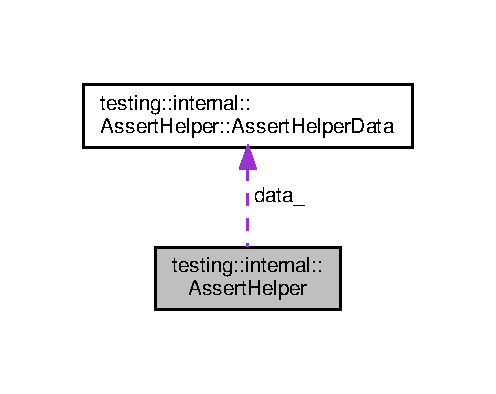
\includegraphics[width=238pt]{classtesting_1_1internal_1_1AssertHelper__coll__graph}
\end{center}
\end{figure}
\subsection*{Classes}
\begin{DoxyCompactItemize}
\item 
struct \hyperlink{structtesting_1_1internal_1_1AssertHelper_1_1AssertHelperData}{Assert\+Helper\+Data}
\end{DoxyCompactItemize}
\subsection*{Public Member Functions}
\begin{DoxyCompactItemize}
\item 
\hyperlink{classtesting_1_1internal_1_1AssertHelper_ac2c9334518fd4087189b4505567a3c90}{Assert\+Helper} (Test\+Part\+Result\+::\+Type type, const char $\ast$file, int line, const char $\ast$message)
\item 
\hyperlink{classtesting_1_1internal_1_1AssertHelper_a51c640785d4ed4a0155cc9aa857d8931}{$\sim$\+Assert\+Helper} ()
\item 
void \hyperlink{classtesting_1_1internal_1_1AssertHelper_a97bf22d786131ab7baa86b97a27aeb4d}{operator=} (const \hyperlink{classtesting_1_1Message}{Message} \&message) const
\end{DoxyCompactItemize}
\subsection*{Private Member Functions}
\begin{DoxyCompactItemize}
\item 
\hyperlink{classtesting_1_1internal_1_1AssertHelper_a264544ac41950b296c34253d2e656b10}{G\+T\+E\+S\+T\+\_\+\+D\+I\+S\+A\+L\+L\+O\+W\+\_\+\+C\+O\+P\+Y\+\_\+\+A\+N\+D\+\_\+\+A\+S\+S\+I\+G\+N\+\_\+} (\hyperlink{classtesting_1_1internal_1_1AssertHelper}{Assert\+Helper})
\end{DoxyCompactItemize}
\subsection*{Private Attributes}
\begin{DoxyCompactItemize}
\item 
\hyperlink{structtesting_1_1internal_1_1AssertHelper_1_1AssertHelperData}{Assert\+Helper\+Data} $\ast$const \hyperlink{classtesting_1_1internal_1_1AssertHelper_af69a4d66a929d0c6e419f4efd3ba6b3a}{data\+\_\+}
\end{DoxyCompactItemize}


\subsection{Constructor \& Destructor Documentation}
\mbox{\Hypertarget{classtesting_1_1internal_1_1AssertHelper_ac2c9334518fd4087189b4505567a3c90}\label{classtesting_1_1internal_1_1AssertHelper_ac2c9334518fd4087189b4505567a3c90}} 
\index{testing\+::internal\+::\+Assert\+Helper@{testing\+::internal\+::\+Assert\+Helper}!Assert\+Helper@{Assert\+Helper}}
\index{Assert\+Helper@{Assert\+Helper}!testing\+::internal\+::\+Assert\+Helper@{testing\+::internal\+::\+Assert\+Helper}}
\subsubsection{\texorpdfstring{Assert\+Helper()}{AssertHelper()}}
{\footnotesize\ttfamily testing\+::internal\+::\+Assert\+Helper\+::\+Assert\+Helper (\begin{DoxyParamCaption}\item[{Test\+Part\+Result\+::\+Type}]{type,  }\item[{const char $\ast$}]{file,  }\item[{int}]{line,  }\item[{const char $\ast$}]{message }\end{DoxyParamCaption})}

\mbox{\Hypertarget{classtesting_1_1internal_1_1AssertHelper_a51c640785d4ed4a0155cc9aa857d8931}\label{classtesting_1_1internal_1_1AssertHelper_a51c640785d4ed4a0155cc9aa857d8931}} 
\index{testing\+::internal\+::\+Assert\+Helper@{testing\+::internal\+::\+Assert\+Helper}!````~Assert\+Helper@{$\sim$\+Assert\+Helper}}
\index{````~Assert\+Helper@{$\sim$\+Assert\+Helper}!testing\+::internal\+::\+Assert\+Helper@{testing\+::internal\+::\+Assert\+Helper}}
\subsubsection{\texorpdfstring{$\sim$\+Assert\+Helper()}{~AssertHelper()}}
{\footnotesize\ttfamily testing\+::internal\+::\+Assert\+Helper\+::$\sim$\+Assert\+Helper (\begin{DoxyParamCaption}{ }\end{DoxyParamCaption})}



\subsection{Member Function Documentation}
\mbox{\Hypertarget{classtesting_1_1internal_1_1AssertHelper_a264544ac41950b296c34253d2e656b10}\label{classtesting_1_1internal_1_1AssertHelper_a264544ac41950b296c34253d2e656b10}} 
\index{testing\+::internal\+::\+Assert\+Helper@{testing\+::internal\+::\+Assert\+Helper}!G\+T\+E\+S\+T\+\_\+\+D\+I\+S\+A\+L\+L\+O\+W\+\_\+\+C\+O\+P\+Y\+\_\+\+A\+N\+D\+\_\+\+A\+S\+S\+I\+G\+N\+\_\+@{G\+T\+E\+S\+T\+\_\+\+D\+I\+S\+A\+L\+L\+O\+W\+\_\+\+C\+O\+P\+Y\+\_\+\+A\+N\+D\+\_\+\+A\+S\+S\+I\+G\+N\+\_\+}}
\index{G\+T\+E\+S\+T\+\_\+\+D\+I\+S\+A\+L\+L\+O\+W\+\_\+\+C\+O\+P\+Y\+\_\+\+A\+N\+D\+\_\+\+A\+S\+S\+I\+G\+N\+\_\+@{G\+T\+E\+S\+T\+\_\+\+D\+I\+S\+A\+L\+L\+O\+W\+\_\+\+C\+O\+P\+Y\+\_\+\+A\+N\+D\+\_\+\+A\+S\+S\+I\+G\+N\+\_\+}!testing\+::internal\+::\+Assert\+Helper@{testing\+::internal\+::\+Assert\+Helper}}
\subsubsection{\texorpdfstring{G\+T\+E\+S\+T\+\_\+\+D\+I\+S\+A\+L\+L\+O\+W\+\_\+\+C\+O\+P\+Y\+\_\+\+A\+N\+D\+\_\+\+A\+S\+S\+I\+G\+N\+\_\+()}{GTEST\_DISALLOW\_COPY\_AND\_ASSIGN\_()}}
{\footnotesize\ttfamily testing\+::internal\+::\+Assert\+Helper\+::\+G\+T\+E\+S\+T\+\_\+\+D\+I\+S\+A\+L\+L\+O\+W\+\_\+\+C\+O\+P\+Y\+\_\+\+A\+N\+D\+\_\+\+A\+S\+S\+I\+G\+N\+\_\+ (\begin{DoxyParamCaption}\item[{\hyperlink{classtesting_1_1internal_1_1AssertHelper}{Assert\+Helper}}]{ }\end{DoxyParamCaption})\hspace{0.3cm}{\ttfamily [private]}}

\mbox{\Hypertarget{classtesting_1_1internal_1_1AssertHelper_a97bf22d786131ab7baa86b97a27aeb4d}\label{classtesting_1_1internal_1_1AssertHelper_a97bf22d786131ab7baa86b97a27aeb4d}} 
\index{testing\+::internal\+::\+Assert\+Helper@{testing\+::internal\+::\+Assert\+Helper}!operator=@{operator=}}
\index{operator=@{operator=}!testing\+::internal\+::\+Assert\+Helper@{testing\+::internal\+::\+Assert\+Helper}}
\subsubsection{\texorpdfstring{operator=()}{operator=()}}
{\footnotesize\ttfamily void testing\+::internal\+::\+Assert\+Helper\+::operator= (\begin{DoxyParamCaption}\item[{const \hyperlink{classtesting_1_1Message}{Message} \&}]{message }\end{DoxyParamCaption}) const}



\subsection{Member Data Documentation}
\mbox{\Hypertarget{classtesting_1_1internal_1_1AssertHelper_af69a4d66a929d0c6e419f4efd3ba6b3a}\label{classtesting_1_1internal_1_1AssertHelper_af69a4d66a929d0c6e419f4efd3ba6b3a}} 
\index{testing\+::internal\+::\+Assert\+Helper@{testing\+::internal\+::\+Assert\+Helper}!data\+\_\+@{data\+\_\+}}
\index{data\+\_\+@{data\+\_\+}!testing\+::internal\+::\+Assert\+Helper@{testing\+::internal\+::\+Assert\+Helper}}
\subsubsection{\texorpdfstring{data\+\_\+}{data\_}}
{\footnotesize\ttfamily \hyperlink{structtesting_1_1internal_1_1AssertHelper_1_1AssertHelperData}{Assert\+Helper\+Data}$\ast$ const testing\+::internal\+::\+Assert\+Helper\+::data\+\_\+\hspace{0.3cm}{\ttfamily [private]}}



The documentation for this class was generated from the following file\+:\begin{DoxyCompactItemize}
\item 
tests/googletest/include/gtest/\hyperlink{gtest_8h}{gtest.\+h}\end{DoxyCompactItemize}

\hypertarget{structtesting_1_1internal_1_1AssertHelper_1_1AssertHelperData}{}\section{testing\+:\+:internal\+:\+:Assert\+Helper\+:\+:Assert\+Helper\+Data Struct Reference}
\label{structtesting_1_1internal_1_1AssertHelper_1_1AssertHelperData}\index{testing\+::internal\+::\+Assert\+Helper\+::\+Assert\+Helper\+Data@{testing\+::internal\+::\+Assert\+Helper\+::\+Assert\+Helper\+Data}}
\subsection*{Public Member Functions}
\begin{DoxyCompactItemize}
\item 
\hyperlink{structtesting_1_1internal_1_1AssertHelper_1_1AssertHelperData_ad2356f3f1e56d1a63562efe0f8b3f1bb}{Assert\+Helper\+Data} (Test\+Part\+Result\+::\+Type t, const char $\ast$srcfile, int line\+\_\+num, const char $\ast$msg)
\end{DoxyCompactItemize}
\subsection*{Public Attributes}
\begin{DoxyCompactItemize}
\item 
Test\+Part\+Result\+::\+Type const \hyperlink{structtesting_1_1internal_1_1AssertHelper_1_1AssertHelperData_a7b1d1a77882cd82107acea856d45692f}{type}
\item 
const char $\ast$const \hyperlink{structtesting_1_1internal_1_1AssertHelper_1_1AssertHelperData_a639ae4acc706e919b101786f71e9dc15}{file}
\item 
int const \hyperlink{structtesting_1_1internal_1_1AssertHelper_1_1AssertHelperData_aff816673320ecd035288dffe44760f90}{line}
\item 
std\+::string const \hyperlink{structtesting_1_1internal_1_1AssertHelper_1_1AssertHelperData_ae81536d57b8deb5dca4159cc6f7efdf0}{message}
\end{DoxyCompactItemize}
\subsection*{Private Member Functions}
\begin{DoxyCompactItemize}
\item 
\hyperlink{structtesting_1_1internal_1_1AssertHelper_1_1AssertHelperData_a5cfdd2fca371e33566ffdb2357606df2}{G\+T\+E\+S\+T\+\_\+\+D\+I\+S\+A\+L\+L\+O\+W\+\_\+\+C\+O\+P\+Y\+\_\+\+A\+N\+D\+\_\+\+A\+S\+S\+I\+G\+N\+\_\+} (\hyperlink{structtesting_1_1internal_1_1AssertHelper_1_1AssertHelperData}{Assert\+Helper\+Data})
\end{DoxyCompactItemize}


\subsection{Constructor \& Destructor Documentation}
\mbox{\Hypertarget{structtesting_1_1internal_1_1AssertHelper_1_1AssertHelperData_ad2356f3f1e56d1a63562efe0f8b3f1bb}\label{structtesting_1_1internal_1_1AssertHelper_1_1AssertHelperData_ad2356f3f1e56d1a63562efe0f8b3f1bb}} 
\index{testing\+::internal\+::\+Assert\+Helper\+::\+Assert\+Helper\+Data@{testing\+::internal\+::\+Assert\+Helper\+::\+Assert\+Helper\+Data}!Assert\+Helper\+Data@{Assert\+Helper\+Data}}
\index{Assert\+Helper\+Data@{Assert\+Helper\+Data}!testing\+::internal\+::\+Assert\+Helper\+::\+Assert\+Helper\+Data@{testing\+::internal\+::\+Assert\+Helper\+::\+Assert\+Helper\+Data}}
\subsubsection{\texorpdfstring{Assert\+Helper\+Data()}{AssertHelperData()}}
{\footnotesize\ttfamily testing\+::internal\+::\+Assert\+Helper\+::\+Assert\+Helper\+Data\+::\+Assert\+Helper\+Data (\begin{DoxyParamCaption}\item[{Test\+Part\+Result\+::\+Type}]{t,  }\item[{const char $\ast$}]{srcfile,  }\item[{int}]{line\+\_\+num,  }\item[{const char $\ast$}]{msg }\end{DoxyParamCaption})\hspace{0.3cm}{\ttfamily [inline]}}



\subsection{Member Function Documentation}
\mbox{\Hypertarget{structtesting_1_1internal_1_1AssertHelper_1_1AssertHelperData_a5cfdd2fca371e33566ffdb2357606df2}\label{structtesting_1_1internal_1_1AssertHelper_1_1AssertHelperData_a5cfdd2fca371e33566ffdb2357606df2}} 
\index{testing\+::internal\+::\+Assert\+Helper\+::\+Assert\+Helper\+Data@{testing\+::internal\+::\+Assert\+Helper\+::\+Assert\+Helper\+Data}!G\+T\+E\+S\+T\+\_\+\+D\+I\+S\+A\+L\+L\+O\+W\+\_\+\+C\+O\+P\+Y\+\_\+\+A\+N\+D\+\_\+\+A\+S\+S\+I\+G\+N\+\_\+@{G\+T\+E\+S\+T\+\_\+\+D\+I\+S\+A\+L\+L\+O\+W\+\_\+\+C\+O\+P\+Y\+\_\+\+A\+N\+D\+\_\+\+A\+S\+S\+I\+G\+N\+\_\+}}
\index{G\+T\+E\+S\+T\+\_\+\+D\+I\+S\+A\+L\+L\+O\+W\+\_\+\+C\+O\+P\+Y\+\_\+\+A\+N\+D\+\_\+\+A\+S\+S\+I\+G\+N\+\_\+@{G\+T\+E\+S\+T\+\_\+\+D\+I\+S\+A\+L\+L\+O\+W\+\_\+\+C\+O\+P\+Y\+\_\+\+A\+N\+D\+\_\+\+A\+S\+S\+I\+G\+N\+\_\+}!testing\+::internal\+::\+Assert\+Helper\+::\+Assert\+Helper\+Data@{testing\+::internal\+::\+Assert\+Helper\+::\+Assert\+Helper\+Data}}
\subsubsection{\texorpdfstring{G\+T\+E\+S\+T\+\_\+\+D\+I\+S\+A\+L\+L\+O\+W\+\_\+\+C\+O\+P\+Y\+\_\+\+A\+N\+D\+\_\+\+A\+S\+S\+I\+G\+N\+\_\+()}{GTEST\_DISALLOW\_COPY\_AND\_ASSIGN\_()}}
{\footnotesize\ttfamily testing\+::internal\+::\+Assert\+Helper\+::\+Assert\+Helper\+Data\+::\+G\+T\+E\+S\+T\+\_\+\+D\+I\+S\+A\+L\+L\+O\+W\+\_\+\+C\+O\+P\+Y\+\_\+\+A\+N\+D\+\_\+\+A\+S\+S\+I\+G\+N\+\_\+ (\begin{DoxyParamCaption}\item[{\hyperlink{structtesting_1_1internal_1_1AssertHelper_1_1AssertHelperData}{Assert\+Helper\+Data}}]{ }\end{DoxyParamCaption})\hspace{0.3cm}{\ttfamily [private]}}



\subsection{Member Data Documentation}
\mbox{\Hypertarget{structtesting_1_1internal_1_1AssertHelper_1_1AssertHelperData_a639ae4acc706e919b101786f71e9dc15}\label{structtesting_1_1internal_1_1AssertHelper_1_1AssertHelperData_a639ae4acc706e919b101786f71e9dc15}} 
\index{testing\+::internal\+::\+Assert\+Helper\+::\+Assert\+Helper\+Data@{testing\+::internal\+::\+Assert\+Helper\+::\+Assert\+Helper\+Data}!file@{file}}
\index{file@{file}!testing\+::internal\+::\+Assert\+Helper\+::\+Assert\+Helper\+Data@{testing\+::internal\+::\+Assert\+Helper\+::\+Assert\+Helper\+Data}}
\subsubsection{\texorpdfstring{file}{file}}
{\footnotesize\ttfamily const char$\ast$ const testing\+::internal\+::\+Assert\+Helper\+::\+Assert\+Helper\+Data\+::file}

\mbox{\Hypertarget{structtesting_1_1internal_1_1AssertHelper_1_1AssertHelperData_aff816673320ecd035288dffe44760f90}\label{structtesting_1_1internal_1_1AssertHelper_1_1AssertHelperData_aff816673320ecd035288dffe44760f90}} 
\index{testing\+::internal\+::\+Assert\+Helper\+::\+Assert\+Helper\+Data@{testing\+::internal\+::\+Assert\+Helper\+::\+Assert\+Helper\+Data}!line@{line}}
\index{line@{line}!testing\+::internal\+::\+Assert\+Helper\+::\+Assert\+Helper\+Data@{testing\+::internal\+::\+Assert\+Helper\+::\+Assert\+Helper\+Data}}
\subsubsection{\texorpdfstring{line}{line}}
{\footnotesize\ttfamily int const testing\+::internal\+::\+Assert\+Helper\+::\+Assert\+Helper\+Data\+::line}

\mbox{\Hypertarget{structtesting_1_1internal_1_1AssertHelper_1_1AssertHelperData_ae81536d57b8deb5dca4159cc6f7efdf0}\label{structtesting_1_1internal_1_1AssertHelper_1_1AssertHelperData_ae81536d57b8deb5dca4159cc6f7efdf0}} 
\index{testing\+::internal\+::\+Assert\+Helper\+::\+Assert\+Helper\+Data@{testing\+::internal\+::\+Assert\+Helper\+::\+Assert\+Helper\+Data}!message@{message}}
\index{message@{message}!testing\+::internal\+::\+Assert\+Helper\+::\+Assert\+Helper\+Data@{testing\+::internal\+::\+Assert\+Helper\+::\+Assert\+Helper\+Data}}
\subsubsection{\texorpdfstring{message}{message}}
{\footnotesize\ttfamily std\+::string const testing\+::internal\+::\+Assert\+Helper\+::\+Assert\+Helper\+Data\+::message}

\mbox{\Hypertarget{structtesting_1_1internal_1_1AssertHelper_1_1AssertHelperData_a7b1d1a77882cd82107acea856d45692f}\label{structtesting_1_1internal_1_1AssertHelper_1_1AssertHelperData_a7b1d1a77882cd82107acea856d45692f}} 
\index{testing\+::internal\+::\+Assert\+Helper\+::\+Assert\+Helper\+Data@{testing\+::internal\+::\+Assert\+Helper\+::\+Assert\+Helper\+Data}!type@{type}}
\index{type@{type}!testing\+::internal\+::\+Assert\+Helper\+::\+Assert\+Helper\+Data@{testing\+::internal\+::\+Assert\+Helper\+::\+Assert\+Helper\+Data}}
\subsubsection{\texorpdfstring{type}{type}}
{\footnotesize\ttfamily Test\+Part\+Result\+::\+Type const testing\+::internal\+::\+Assert\+Helper\+::\+Assert\+Helper\+Data\+::type}



The documentation for this struct was generated from the following file\+:\begin{DoxyCompactItemize}
\item 
tests/googletest/include/gtest/\hyperlink{gtest_8h}{gtest.\+h}\end{DoxyCompactItemize}

\hypertarget{structtesting_1_1internal_1_1bool__constant}{}\section{testing\+:\+:internal\+:\+:bool\+\_\+constant$<$ bool\+\_\+value $>$ Struct Template Reference}
\label{structtesting_1_1internal_1_1bool__constant}\index{testing\+::internal\+::bool\+\_\+constant$<$ bool\+\_\+value $>$@{testing\+::internal\+::bool\+\_\+constant$<$ bool\+\_\+value $>$}}


{\ttfamily \#include $<$gtest-\/port.\+h$>$}



Inheritance diagram for testing\+:\+:internal\+:\+:bool\+\_\+constant$<$ bool\+\_\+value $>$\+:\nopagebreak
\begin{figure}[H]
\begin{center}
\leavevmode
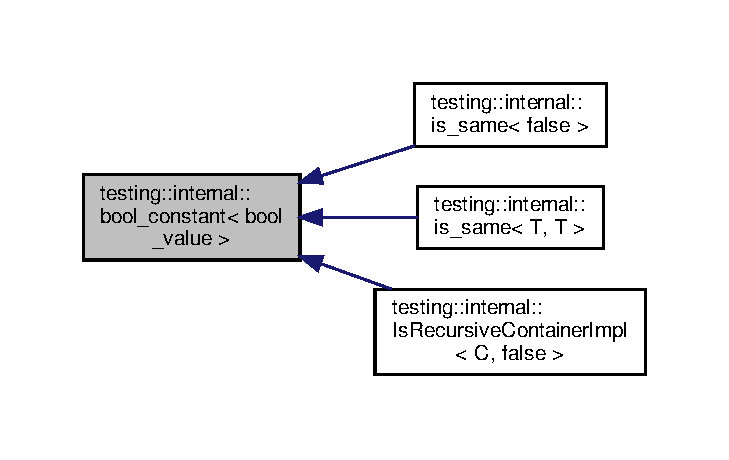
\includegraphics[width=350pt]{structtesting_1_1internal_1_1bool__constant__inherit__graph}
\end{center}
\end{figure}
\subsection*{Public Types}
\begin{DoxyCompactItemize}
\item 
typedef \hyperlink{structtesting_1_1internal_1_1bool__constant}{bool\+\_\+constant}$<$ bool\+\_\+value $>$ \hyperlink{structtesting_1_1internal_1_1bool__constant_aba6d09ecf7eecea6c93480f0d627a167}{type}
\end{DoxyCompactItemize}
\subsection*{Static Public Attributes}
\begin{DoxyCompactItemize}
\item 
static const bool \hyperlink{structtesting_1_1internal_1_1bool__constant_a499fba6576296b04d99690a486424b32}{value} = bool\+\_\+value
\end{DoxyCompactItemize}


\subsection{Member Typedef Documentation}
\mbox{\Hypertarget{structtesting_1_1internal_1_1bool__constant_aba6d09ecf7eecea6c93480f0d627a167}\label{structtesting_1_1internal_1_1bool__constant_aba6d09ecf7eecea6c93480f0d627a167}} 
\index{testing\+::internal\+::bool\+\_\+constant@{testing\+::internal\+::bool\+\_\+constant}!type@{type}}
\index{type@{type}!testing\+::internal\+::bool\+\_\+constant@{testing\+::internal\+::bool\+\_\+constant}}
\subsubsection{\texorpdfstring{type}{type}}
{\footnotesize\ttfamily template$<$bool bool\+\_\+value$>$ \\
typedef \hyperlink{structtesting_1_1internal_1_1bool__constant}{bool\+\_\+constant}$<$bool\+\_\+value$>$ \hyperlink{structtesting_1_1internal_1_1bool__constant}{testing\+::internal\+::bool\+\_\+constant}$<$ bool\+\_\+value $>$\+::\hyperlink{structtesting_1_1internal_1_1bool__constant_aba6d09ecf7eecea6c93480f0d627a167}{type}}



\subsection{Member Data Documentation}
\mbox{\Hypertarget{structtesting_1_1internal_1_1bool__constant_a499fba6576296b04d99690a486424b32}\label{structtesting_1_1internal_1_1bool__constant_a499fba6576296b04d99690a486424b32}} 
\index{testing\+::internal\+::bool\+\_\+constant@{testing\+::internal\+::bool\+\_\+constant}!value@{value}}
\index{value@{value}!testing\+::internal\+::bool\+\_\+constant@{testing\+::internal\+::bool\+\_\+constant}}
\subsubsection{\texorpdfstring{value}{value}}
{\footnotesize\ttfamily template$<$bool bool\+\_\+value$>$ \\
const bool \hyperlink{structtesting_1_1internal_1_1bool__constant}{testing\+::internal\+::bool\+\_\+constant}$<$ bool\+\_\+value $>$\+::value = bool\+\_\+value\hspace{0.3cm}{\ttfamily [static]}}



The documentation for this struct was generated from the following file\+:\begin{DoxyCompactItemize}
\item 
tests/googletest/include/gtest/internal/\hyperlink{gtest-port_8h}{gtest-\/port.\+h}\end{DoxyCompactItemize}

\hypertarget{classtesting_1_1internal_1_1CartesianProductGenerator}{}\section{testing\+:\+:internal\+:\+:Cartesian\+Product\+Generator$<$ T $>$ Class Template Reference}
\label{classtesting_1_1internal_1_1CartesianProductGenerator}\index{testing\+::internal\+::\+Cartesian\+Product\+Generator$<$ T $>$@{testing\+::internal\+::\+Cartesian\+Product\+Generator$<$ T $>$}}


{\ttfamily \#include $<$gtest-\/param-\/util.\+h$>$}



Inheritance diagram for testing\+:\+:internal\+:\+:Cartesian\+Product\+Generator$<$ T $>$\+:\nopagebreak
\begin{figure}[H]
\begin{center}
\leavevmode
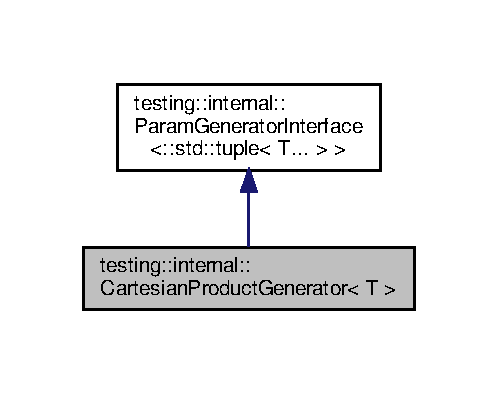
\includegraphics[width=239pt]{classtesting_1_1internal_1_1CartesianProductGenerator__inherit__graph}
\end{center}
\end{figure}


Collaboration diagram for testing\+:\+:internal\+:\+:Cartesian\+Product\+Generator$<$ T $>$\+:\nopagebreak
\begin{figure}[H]
\begin{center}
\leavevmode
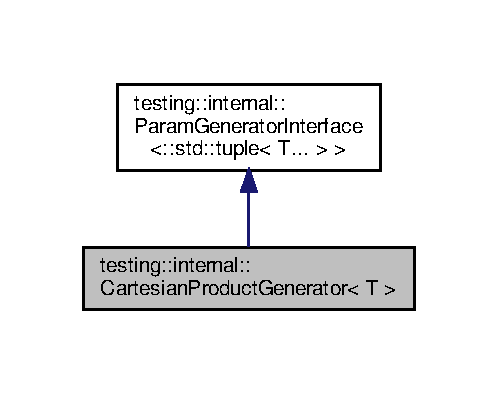
\includegraphics[width=239pt]{classtesting_1_1internal_1_1CartesianProductGenerator__coll__graph}
\end{center}
\end{figure}
\subsection*{Classes}
\begin{DoxyCompactItemize}
\item 
class \hyperlink{classtesting_1_1internal_1_1CartesianProductGenerator_1_1IteratorImpl}{Iterator\+Impl}
\item 
class \hyperlink{classtesting_1_1internal_1_1CartesianProductGenerator_1_1IteratorImpl_3_01IndexSequence_3_01I_8_8_8_01_4_01_4}{Iterator\+Impl$<$ Index\+Sequence$<$ I... $>$ $>$}
\end{DoxyCompactItemize}
\subsection*{Public Types}
\begin{DoxyCompactItemize}
\item 
typedef \+::std\+::tuple$<$ T... $>$ \hyperlink{classtesting_1_1internal_1_1CartesianProductGenerator_af27131157a9347f0c82420ca081ee7dd}{Param\+Type}
\end{DoxyCompactItemize}
\subsection*{Public Member Functions}
\begin{DoxyCompactItemize}
\item 
\hyperlink{classtesting_1_1internal_1_1CartesianProductGenerator_af89630ce27d49f999f323e6c3d2867af}{Cartesian\+Product\+Generator} (const std\+::tuple$<$ \hyperlink{classtesting_1_1internal_1_1ParamGenerator}{Param\+Generator}$<$ T $>$... $>$ \&g)
\item 
\hyperlink{classtesting_1_1internal_1_1CartesianProductGenerator_a19fb6a9435f038520cef7643fdf6da71}{$\sim$\+Cartesian\+Product\+Generator} () override
\item 
\hyperlink{classtesting_1_1internal_1_1ParamIteratorInterface}{Param\+Iterator\+Interface}$<$ \hyperlink{classtesting_1_1internal_1_1CartesianProductGenerator_af27131157a9347f0c82420ca081ee7dd}{Param\+Type} $>$ $\ast$ \hyperlink{classtesting_1_1internal_1_1CartesianProductGenerator_ad2f1bc6289b6dd7e4b5f4fecbfdf2883}{Begin} () const override
\item 
\hyperlink{classtesting_1_1internal_1_1ParamIteratorInterface}{Param\+Iterator\+Interface}$<$ \hyperlink{classtesting_1_1internal_1_1CartesianProductGenerator_af27131157a9347f0c82420ca081ee7dd}{Param\+Type} $>$ $\ast$ \hyperlink{classtesting_1_1internal_1_1CartesianProductGenerator_ae072dcf8400ac9dd5692e417262a664b}{End} () const override
\end{DoxyCompactItemize}
\subsection*{Private Types}
\begin{DoxyCompactItemize}
\item 
using \hyperlink{classtesting_1_1internal_1_1CartesianProductGenerator_a01d41f7e7634ce6c4408af397f86bce3}{Iterator} = \hyperlink{classtesting_1_1internal_1_1CartesianProductGenerator_1_1IteratorImpl}{Iterator\+Impl}$<$ typename \hyperlink{structtesting_1_1internal_1_1MakeIndexSequence}{Make\+Index\+Sequence}$<$ sizeof...(T)$>$\+::type $>$
\end{DoxyCompactItemize}
\subsection*{Private Attributes}
\begin{DoxyCompactItemize}
\item 
std\+::tuple$<$ \hyperlink{classtesting_1_1internal_1_1ParamGenerator}{Param\+Generator}$<$ T $>$... $>$ \hyperlink{classtesting_1_1internal_1_1CartesianProductGenerator_adb1f110ba803c09b0b1c38b7602652b1}{generators\+\_\+}
\end{DoxyCompactItemize}


\subsection{Member Typedef Documentation}
\mbox{\Hypertarget{classtesting_1_1internal_1_1CartesianProductGenerator_a01d41f7e7634ce6c4408af397f86bce3}\label{classtesting_1_1internal_1_1CartesianProductGenerator_a01d41f7e7634ce6c4408af397f86bce3}} 
\index{testing\+::internal\+::\+Cartesian\+Product\+Generator@{testing\+::internal\+::\+Cartesian\+Product\+Generator}!Iterator@{Iterator}}
\index{Iterator@{Iterator}!testing\+::internal\+::\+Cartesian\+Product\+Generator@{testing\+::internal\+::\+Cartesian\+Product\+Generator}}
\subsubsection{\texorpdfstring{Iterator}{Iterator}}
{\footnotesize\ttfamily template$<$typename... T$>$ \\
using \hyperlink{classtesting_1_1internal_1_1CartesianProductGenerator}{testing\+::internal\+::\+Cartesian\+Product\+Generator}$<$ T $>$\+::\hyperlink{classtesting_1_1internal_1_1CartesianProductGenerator_a01d41f7e7634ce6c4408af397f86bce3}{Iterator} =  \hyperlink{classtesting_1_1internal_1_1CartesianProductGenerator_1_1IteratorImpl}{Iterator\+Impl}$<$typename \hyperlink{structtesting_1_1internal_1_1MakeIndexSequence}{Make\+Index\+Sequence}$<$sizeof...(T)$>$\+::type$>$\hspace{0.3cm}{\ttfamily [private]}}

\mbox{\Hypertarget{classtesting_1_1internal_1_1CartesianProductGenerator_af27131157a9347f0c82420ca081ee7dd}\label{classtesting_1_1internal_1_1CartesianProductGenerator_af27131157a9347f0c82420ca081ee7dd}} 
\index{testing\+::internal\+::\+Cartesian\+Product\+Generator@{testing\+::internal\+::\+Cartesian\+Product\+Generator}!Param\+Type@{Param\+Type}}
\index{Param\+Type@{Param\+Type}!testing\+::internal\+::\+Cartesian\+Product\+Generator@{testing\+::internal\+::\+Cartesian\+Product\+Generator}}
\subsubsection{\texorpdfstring{Param\+Type}{ParamType}}
{\footnotesize\ttfamily template$<$typename... T$>$ \\
typedef \+::std\+::tuple$<$T...$>$ \hyperlink{classtesting_1_1internal_1_1CartesianProductGenerator}{testing\+::internal\+::\+Cartesian\+Product\+Generator}$<$ T $>$\+::\hyperlink{classtesting_1_1internal_1_1CartesianProductGenerator_af27131157a9347f0c82420ca081ee7dd}{Param\+Type}}



\subsection{Constructor \& Destructor Documentation}
\mbox{\Hypertarget{classtesting_1_1internal_1_1CartesianProductGenerator_af89630ce27d49f999f323e6c3d2867af}\label{classtesting_1_1internal_1_1CartesianProductGenerator_af89630ce27d49f999f323e6c3d2867af}} 
\index{testing\+::internal\+::\+Cartesian\+Product\+Generator@{testing\+::internal\+::\+Cartesian\+Product\+Generator}!Cartesian\+Product\+Generator@{Cartesian\+Product\+Generator}}
\index{Cartesian\+Product\+Generator@{Cartesian\+Product\+Generator}!testing\+::internal\+::\+Cartesian\+Product\+Generator@{testing\+::internal\+::\+Cartesian\+Product\+Generator}}
\subsubsection{\texorpdfstring{Cartesian\+Product\+Generator()}{CartesianProductGenerator()}}
{\footnotesize\ttfamily template$<$typename... T$>$ \\
\hyperlink{classtesting_1_1internal_1_1CartesianProductGenerator}{testing\+::internal\+::\+Cartesian\+Product\+Generator}$<$ T $>$\+::\hyperlink{classtesting_1_1internal_1_1CartesianProductGenerator}{Cartesian\+Product\+Generator} (\begin{DoxyParamCaption}\item[{const std\+::tuple$<$ \hyperlink{classtesting_1_1internal_1_1ParamGenerator}{Param\+Generator}$<$ T $>$... $>$ \&}]{g }\end{DoxyParamCaption})\hspace{0.3cm}{\ttfamily [inline]}}

\mbox{\Hypertarget{classtesting_1_1internal_1_1CartesianProductGenerator_a19fb6a9435f038520cef7643fdf6da71}\label{classtesting_1_1internal_1_1CartesianProductGenerator_a19fb6a9435f038520cef7643fdf6da71}} 
\index{testing\+::internal\+::\+Cartesian\+Product\+Generator@{testing\+::internal\+::\+Cartesian\+Product\+Generator}!````~Cartesian\+Product\+Generator@{$\sim$\+Cartesian\+Product\+Generator}}
\index{````~Cartesian\+Product\+Generator@{$\sim$\+Cartesian\+Product\+Generator}!testing\+::internal\+::\+Cartesian\+Product\+Generator@{testing\+::internal\+::\+Cartesian\+Product\+Generator}}
\subsubsection{\texorpdfstring{$\sim$\+Cartesian\+Product\+Generator()}{~CartesianProductGenerator()}}
{\footnotesize\ttfamily template$<$typename... T$>$ \\
\hyperlink{classtesting_1_1internal_1_1CartesianProductGenerator}{testing\+::internal\+::\+Cartesian\+Product\+Generator}$<$ T $>$\+::$\sim$\hyperlink{classtesting_1_1internal_1_1CartesianProductGenerator}{Cartesian\+Product\+Generator} (\begin{DoxyParamCaption}{ }\end{DoxyParamCaption})\hspace{0.3cm}{\ttfamily [inline]}, {\ttfamily [override]}}



\subsection{Member Function Documentation}
\mbox{\Hypertarget{classtesting_1_1internal_1_1CartesianProductGenerator_ad2f1bc6289b6dd7e4b5f4fecbfdf2883}\label{classtesting_1_1internal_1_1CartesianProductGenerator_ad2f1bc6289b6dd7e4b5f4fecbfdf2883}} 
\index{testing\+::internal\+::\+Cartesian\+Product\+Generator@{testing\+::internal\+::\+Cartesian\+Product\+Generator}!Begin@{Begin}}
\index{Begin@{Begin}!testing\+::internal\+::\+Cartesian\+Product\+Generator@{testing\+::internal\+::\+Cartesian\+Product\+Generator}}
\subsubsection{\texorpdfstring{Begin()}{Begin()}}
{\footnotesize\ttfamily template$<$typename... T$>$ \\
\hyperlink{classtesting_1_1internal_1_1ParamIteratorInterface}{Param\+Iterator\+Interface}$<$\hyperlink{classtesting_1_1internal_1_1CartesianProductGenerator_af27131157a9347f0c82420ca081ee7dd}{Param\+Type}$>$$\ast$ \hyperlink{classtesting_1_1internal_1_1CartesianProductGenerator}{testing\+::internal\+::\+Cartesian\+Product\+Generator}$<$ T $>$\+::Begin (\begin{DoxyParamCaption}{ }\end{DoxyParamCaption}) const\hspace{0.3cm}{\ttfamily [inline]}, {\ttfamily [override]}, {\ttfamily [virtual]}}



Implements \hyperlink{classtesting_1_1internal_1_1ParamGeneratorInterface_ae1de83b16fe9a53c67778a026c6a9569}{testing\+::internal\+::\+Param\+Generator\+Interface$<$\+::std\+::tuple$<$ T... $>$ $>$}.

\mbox{\Hypertarget{classtesting_1_1internal_1_1CartesianProductGenerator_ae072dcf8400ac9dd5692e417262a664b}\label{classtesting_1_1internal_1_1CartesianProductGenerator_ae072dcf8400ac9dd5692e417262a664b}} 
\index{testing\+::internal\+::\+Cartesian\+Product\+Generator@{testing\+::internal\+::\+Cartesian\+Product\+Generator}!End@{End}}
\index{End@{End}!testing\+::internal\+::\+Cartesian\+Product\+Generator@{testing\+::internal\+::\+Cartesian\+Product\+Generator}}
\subsubsection{\texorpdfstring{End()}{End()}}
{\footnotesize\ttfamily template$<$typename... T$>$ \\
\hyperlink{classtesting_1_1internal_1_1ParamIteratorInterface}{Param\+Iterator\+Interface}$<$\hyperlink{classtesting_1_1internal_1_1CartesianProductGenerator_af27131157a9347f0c82420ca081ee7dd}{Param\+Type}$>$$\ast$ \hyperlink{classtesting_1_1internal_1_1CartesianProductGenerator}{testing\+::internal\+::\+Cartesian\+Product\+Generator}$<$ T $>$\+::End (\begin{DoxyParamCaption}{ }\end{DoxyParamCaption}) const\hspace{0.3cm}{\ttfamily [inline]}, {\ttfamily [override]}, {\ttfamily [virtual]}}



Implements \hyperlink{classtesting_1_1internal_1_1ParamGeneratorInterface_afa7211b74990e11d3fc7ad4e7113da4f}{testing\+::internal\+::\+Param\+Generator\+Interface$<$\+::std\+::tuple$<$ T... $>$ $>$}.



\subsection{Member Data Documentation}
\mbox{\Hypertarget{classtesting_1_1internal_1_1CartesianProductGenerator_adb1f110ba803c09b0b1c38b7602652b1}\label{classtesting_1_1internal_1_1CartesianProductGenerator_adb1f110ba803c09b0b1c38b7602652b1}} 
\index{testing\+::internal\+::\+Cartesian\+Product\+Generator@{testing\+::internal\+::\+Cartesian\+Product\+Generator}!generators\+\_\+@{generators\+\_\+}}
\index{generators\+\_\+@{generators\+\_\+}!testing\+::internal\+::\+Cartesian\+Product\+Generator@{testing\+::internal\+::\+Cartesian\+Product\+Generator}}
\subsubsection{\texorpdfstring{generators\+\_\+}{generators\_}}
{\footnotesize\ttfamily template$<$typename... T$>$ \\
std\+::tuple$<$\hyperlink{classtesting_1_1internal_1_1ParamGenerator}{Param\+Generator}$<$T$>$...$>$ \hyperlink{classtesting_1_1internal_1_1CartesianProductGenerator}{testing\+::internal\+::\+Cartesian\+Product\+Generator}$<$ T $>$\+::generators\+\_\+\hspace{0.3cm}{\ttfamily [private]}}



The documentation for this class was generated from the following file\+:\begin{DoxyCompactItemize}
\item 
tests/googletest/include/gtest/internal/\hyperlink{gtest-param-util_8h}{gtest-\/param-\/util.\+h}\end{DoxyCompactItemize}

\hypertarget{classtesting_1_1internal_1_1CartesianProductHolder}{}\section{testing\+:\+:internal\+:\+:Cartesian\+Product\+Holder$<$ Gen $>$ Class Template Reference}
\label{classtesting_1_1internal_1_1CartesianProductHolder}\index{testing\+::internal\+::\+Cartesian\+Product\+Holder$<$ Gen $>$@{testing\+::internal\+::\+Cartesian\+Product\+Holder$<$ Gen $>$}}


{\ttfamily \#include $<$gtest-\/param-\/util.\+h$>$}

\subsection*{Public Member Functions}
\begin{DoxyCompactItemize}
\item 
\hyperlink{classtesting_1_1internal_1_1CartesianProductHolder_a3584d073ddbe024d6bc478a988c4111c}{Cartesian\+Product\+Holder} (const Gen \&... g)
\item 
{\footnotesize template$<$typename... T$>$ }\\\hyperlink{classtesting_1_1internal_1_1CartesianProductHolder_ab29313123e08f3fc7111eac6e80351a5}{operator Param\+Generator$<$\+::std\+::tuple$<$ T... $>$$>$} () const
\end{DoxyCompactItemize}
\subsection*{Private Attributes}
\begin{DoxyCompactItemize}
\item 
std\+::tuple$<$ Gen... $>$ \hyperlink{classtesting_1_1internal_1_1CartesianProductHolder_a6efba108d2025dbbce1129506284feaf}{generators\+\_\+}
\end{DoxyCompactItemize}


\subsection{Constructor \& Destructor Documentation}
\mbox{\Hypertarget{classtesting_1_1internal_1_1CartesianProductHolder_a3584d073ddbe024d6bc478a988c4111c}\label{classtesting_1_1internal_1_1CartesianProductHolder_a3584d073ddbe024d6bc478a988c4111c}} 
\index{testing\+::internal\+::\+Cartesian\+Product\+Holder@{testing\+::internal\+::\+Cartesian\+Product\+Holder}!Cartesian\+Product\+Holder@{Cartesian\+Product\+Holder}}
\index{Cartesian\+Product\+Holder@{Cartesian\+Product\+Holder}!testing\+::internal\+::\+Cartesian\+Product\+Holder@{testing\+::internal\+::\+Cartesian\+Product\+Holder}}
\subsubsection{\texorpdfstring{Cartesian\+Product\+Holder()}{CartesianProductHolder()}}
{\footnotesize\ttfamily template$<$class... Gen$>$ \\
\hyperlink{classtesting_1_1internal_1_1CartesianProductHolder}{testing\+::internal\+::\+Cartesian\+Product\+Holder}$<$ Gen $>$\+::\hyperlink{classtesting_1_1internal_1_1CartesianProductHolder}{Cartesian\+Product\+Holder} (\begin{DoxyParamCaption}\item[{const Gen \&...}]{g }\end{DoxyParamCaption})\hspace{0.3cm}{\ttfamily [inline]}}



\subsection{Member Function Documentation}
\mbox{\Hypertarget{classtesting_1_1internal_1_1CartesianProductHolder_ab29313123e08f3fc7111eac6e80351a5}\label{classtesting_1_1internal_1_1CartesianProductHolder_ab29313123e08f3fc7111eac6e80351a5}} 
\index{testing\+::internal\+::\+Cartesian\+Product\+Holder@{testing\+::internal\+::\+Cartesian\+Product\+Holder}!operator Param\+Generator$<$\+::std\+::tuple$<$ T... $>$$>$@{operator Param\+Generator$<$\+::std\+::tuple$<$ T... $>$$>$}}
\index{operator Param\+Generator$<$\+::std\+::tuple$<$ T... $>$$>$@{operator Param\+Generator$<$\+::std\+::tuple$<$ T... $>$$>$}!testing\+::internal\+::\+Cartesian\+Product\+Holder@{testing\+::internal\+::\+Cartesian\+Product\+Holder}}
\subsubsection{\texorpdfstring{operator Param\+Generator$<$\+::std\+::tuple$<$ T... $>$$>$()}{operator ParamGenerator<::std::tuple< T... >>()}}
{\footnotesize\ttfamily template$<$class... Gen$>$ \\
template$<$typename... T$>$ \\
\hyperlink{classtesting_1_1internal_1_1CartesianProductHolder}{testing\+::internal\+::\+Cartesian\+Product\+Holder}$<$ Gen $>$\+::operator \hyperlink{classtesting_1_1internal_1_1ParamGenerator}{Param\+Generator}$<$\+::std\+::tuple$<$ T... $>$$>$ (\begin{DoxyParamCaption}{ }\end{DoxyParamCaption}) const\hspace{0.3cm}{\ttfamily [inline]}}



\subsection{Member Data Documentation}
\mbox{\Hypertarget{classtesting_1_1internal_1_1CartesianProductHolder_a6efba108d2025dbbce1129506284feaf}\label{classtesting_1_1internal_1_1CartesianProductHolder_a6efba108d2025dbbce1129506284feaf}} 
\index{testing\+::internal\+::\+Cartesian\+Product\+Holder@{testing\+::internal\+::\+Cartesian\+Product\+Holder}!generators\+\_\+@{generators\+\_\+}}
\index{generators\+\_\+@{generators\+\_\+}!testing\+::internal\+::\+Cartesian\+Product\+Holder@{testing\+::internal\+::\+Cartesian\+Product\+Holder}}
\subsubsection{\texorpdfstring{generators\+\_\+}{generators\_}}
{\footnotesize\ttfamily template$<$class... Gen$>$ \\
std\+::tuple$<$Gen...$>$ \hyperlink{classtesting_1_1internal_1_1CartesianProductHolder}{testing\+::internal\+::\+Cartesian\+Product\+Holder}$<$ Gen $>$\+::generators\+\_\+\hspace{0.3cm}{\ttfamily [private]}}



The documentation for this class was generated from the following file\+:\begin{DoxyCompactItemize}
\item 
tests/googletest/include/gtest/internal/\hyperlink{gtest-param-util_8h}{gtest-\/param-\/util.\+h}\end{DoxyCompactItemize}

\hypertarget{structtesting_1_1internal_1_1CodeLocation}{}\section{testing\+:\+:internal\+:\+:Code\+Location Struct Reference}
\label{structtesting_1_1internal_1_1CodeLocation}\index{testing\+::internal\+::\+Code\+Location@{testing\+::internal\+::\+Code\+Location}}


{\ttfamily \#include $<$gtest-\/internal.\+h$>$}

\subsection*{Public Member Functions}
\begin{DoxyCompactItemize}
\item 
\hyperlink{structtesting_1_1internal_1_1CodeLocation_a323a11851c81629d632c47b9b767b8ac}{Code\+Location} (const std\+::string \&a\+\_\+file, int a\+\_\+line)
\end{DoxyCompactItemize}
\subsection*{Public Attributes}
\begin{DoxyCompactItemize}
\item 
std\+::string \hyperlink{structtesting_1_1internal_1_1CodeLocation_a38118056ad3c11359920274e393bc6b3}{file}
\item 
int \hyperlink{structtesting_1_1internal_1_1CodeLocation_a01c977c7e8834a05a6d6c40b0c416045}{line}
\end{DoxyCompactItemize}


\subsection{Constructor \& Destructor Documentation}
\mbox{\Hypertarget{structtesting_1_1internal_1_1CodeLocation_a323a11851c81629d632c47b9b767b8ac}\label{structtesting_1_1internal_1_1CodeLocation_a323a11851c81629d632c47b9b767b8ac}} 
\index{testing\+::internal\+::\+Code\+Location@{testing\+::internal\+::\+Code\+Location}!Code\+Location@{Code\+Location}}
\index{Code\+Location@{Code\+Location}!testing\+::internal\+::\+Code\+Location@{testing\+::internal\+::\+Code\+Location}}
\subsubsection{\texorpdfstring{Code\+Location()}{CodeLocation()}}
{\footnotesize\ttfamily testing\+::internal\+::\+Code\+Location\+::\+Code\+Location (\begin{DoxyParamCaption}\item[{const std\+::string \&}]{a\+\_\+file,  }\item[{int}]{a\+\_\+line }\end{DoxyParamCaption})\hspace{0.3cm}{\ttfamily [inline]}}



\subsection{Member Data Documentation}
\mbox{\Hypertarget{structtesting_1_1internal_1_1CodeLocation_a38118056ad3c11359920274e393bc6b3}\label{structtesting_1_1internal_1_1CodeLocation_a38118056ad3c11359920274e393bc6b3}} 
\index{testing\+::internal\+::\+Code\+Location@{testing\+::internal\+::\+Code\+Location}!file@{file}}
\index{file@{file}!testing\+::internal\+::\+Code\+Location@{testing\+::internal\+::\+Code\+Location}}
\subsubsection{\texorpdfstring{file}{file}}
{\footnotesize\ttfamily std\+::string testing\+::internal\+::\+Code\+Location\+::file}

\mbox{\Hypertarget{structtesting_1_1internal_1_1CodeLocation_a01c977c7e8834a05a6d6c40b0c416045}\label{structtesting_1_1internal_1_1CodeLocation_a01c977c7e8834a05a6d6c40b0c416045}} 
\index{testing\+::internal\+::\+Code\+Location@{testing\+::internal\+::\+Code\+Location}!line@{line}}
\index{line@{line}!testing\+::internal\+::\+Code\+Location@{testing\+::internal\+::\+Code\+Location}}
\subsubsection{\texorpdfstring{line}{line}}
{\footnotesize\ttfamily int testing\+::internal\+::\+Code\+Location\+::line}



The documentation for this struct was generated from the following file\+:\begin{DoxyCompactItemize}
\item 
tests/googletest/include/gtest/internal/\hyperlink{gtest-internal_8h}{gtest-\/internal.\+h}\end{DoxyCompactItemize}

\hypertarget{structtesting_1_1internal_1_1CompileAssertTypesEqual}{}\section{testing\+:\+:internal\+:\+:Compile\+Assert\+Types\+Equal$<$ T1, T2 $>$ Struct Template Reference}
\label{structtesting_1_1internal_1_1CompileAssertTypesEqual}\index{testing\+::internal\+::\+Compile\+Assert\+Types\+Equal$<$ T1, T2 $>$@{testing\+::internal\+::\+Compile\+Assert\+Types\+Equal$<$ T1, T2 $>$}}


{\ttfamily \#include $<$gtest-\/internal.\+h$>$}



The documentation for this struct was generated from the following file\+:\begin{DoxyCompactItemize}
\item 
tests/googletest/include/gtest/internal/\hyperlink{gtest-internal_8h}{gtest-\/internal.\+h}\end{DoxyCompactItemize}

\hypertarget{structtesting_1_1internal_1_1CompileAssertTypesEqual_3_01T_00_01T_01_4}{}\section{testing\+:\+:internal\+:\+:Compile\+Assert\+Types\+Equal$<$ T, T $>$ Struct Template Reference}
\label{structtesting_1_1internal_1_1CompileAssertTypesEqual_3_01T_00_01T_01_4}\index{testing\+::internal\+::\+Compile\+Assert\+Types\+Equal$<$ T, T $>$@{testing\+::internal\+::\+Compile\+Assert\+Types\+Equal$<$ T, T $>$}}


{\ttfamily \#include $<$gtest-\/internal.\+h$>$}



The documentation for this struct was generated from the following file\+:\begin{DoxyCompactItemize}
\item 
tests/googletest/include/gtest/internal/\hyperlink{gtest-internal_8h}{gtest-\/internal.\+h}\end{DoxyCompactItemize}

\hypertarget{structtesting_1_1internal_1_1ConstCharPtr}{}\section{testing\+:\+:internal\+:\+:Const\+Char\+Ptr Struct Reference}
\label{structtesting_1_1internal_1_1ConstCharPtr}\index{testing\+::internal\+::\+Const\+Char\+Ptr@{testing\+::internal\+::\+Const\+Char\+Ptr}}


{\ttfamily \#include $<$gtest-\/internal.\+h$>$}

\subsection*{Public Member Functions}
\begin{DoxyCompactItemize}
\item 
\hyperlink{structtesting_1_1internal_1_1ConstCharPtr_ae94f6453fa679d815994eccc63062907}{Const\+Char\+Ptr} (const char $\ast$str)
\item 
\hyperlink{structtesting_1_1internal_1_1ConstCharPtr_a85c8174b5d4db8fe96863509ba767b27}{operator bool} () const
\end{DoxyCompactItemize}
\subsection*{Public Attributes}
\begin{DoxyCompactItemize}
\item 
const char $\ast$ \hyperlink{structtesting_1_1internal_1_1ConstCharPtr_adba40d23d5986904b605946f643cf26e}{value}
\end{DoxyCompactItemize}


\subsection{Constructor \& Destructor Documentation}
\mbox{\Hypertarget{structtesting_1_1internal_1_1ConstCharPtr_ae94f6453fa679d815994eccc63062907}\label{structtesting_1_1internal_1_1ConstCharPtr_ae94f6453fa679d815994eccc63062907}} 
\index{testing\+::internal\+::\+Const\+Char\+Ptr@{testing\+::internal\+::\+Const\+Char\+Ptr}!Const\+Char\+Ptr@{Const\+Char\+Ptr}}
\index{Const\+Char\+Ptr@{Const\+Char\+Ptr}!testing\+::internal\+::\+Const\+Char\+Ptr@{testing\+::internal\+::\+Const\+Char\+Ptr}}
\subsubsection{\texorpdfstring{Const\+Char\+Ptr()}{ConstCharPtr()}}
{\footnotesize\ttfamily testing\+::internal\+::\+Const\+Char\+Ptr\+::\+Const\+Char\+Ptr (\begin{DoxyParamCaption}\item[{const char $\ast$}]{str }\end{DoxyParamCaption})\hspace{0.3cm}{\ttfamily [inline]}}



\subsection{Member Function Documentation}
\mbox{\Hypertarget{structtesting_1_1internal_1_1ConstCharPtr_a85c8174b5d4db8fe96863509ba767b27}\label{structtesting_1_1internal_1_1ConstCharPtr_a85c8174b5d4db8fe96863509ba767b27}} 
\index{testing\+::internal\+::\+Const\+Char\+Ptr@{testing\+::internal\+::\+Const\+Char\+Ptr}!operator bool@{operator bool}}
\index{operator bool@{operator bool}!testing\+::internal\+::\+Const\+Char\+Ptr@{testing\+::internal\+::\+Const\+Char\+Ptr}}
\subsubsection{\texorpdfstring{operator bool()}{operator bool()}}
{\footnotesize\ttfamily testing\+::internal\+::\+Const\+Char\+Ptr\+::operator bool (\begin{DoxyParamCaption}{ }\end{DoxyParamCaption}) const\hspace{0.3cm}{\ttfamily [inline]}}



\subsection{Member Data Documentation}
\mbox{\Hypertarget{structtesting_1_1internal_1_1ConstCharPtr_adba40d23d5986904b605946f643cf26e}\label{structtesting_1_1internal_1_1ConstCharPtr_adba40d23d5986904b605946f643cf26e}} 
\index{testing\+::internal\+::\+Const\+Char\+Ptr@{testing\+::internal\+::\+Const\+Char\+Ptr}!value@{value}}
\index{value@{value}!testing\+::internal\+::\+Const\+Char\+Ptr@{testing\+::internal\+::\+Const\+Char\+Ptr}}
\subsubsection{\texorpdfstring{value}{value}}
{\footnotesize\ttfamily const char$\ast$ testing\+::internal\+::\+Const\+Char\+Ptr\+::value}



The documentation for this struct was generated from the following file\+:\begin{DoxyCompactItemize}
\item 
tests/googletest/include/gtest/internal/\hyperlink{gtest-internal_8h}{gtest-\/internal.\+h}\end{DoxyCompactItemize}

\hypertarget{structtesting_1_1internal_1_1ConstRef}{}\section{testing\+:\+:internal\+:\+:Const\+Ref$<$ T $>$ Struct Template Reference}
\label{structtesting_1_1internal_1_1ConstRef}\index{testing\+::internal\+::\+Const\+Ref$<$ T $>$@{testing\+::internal\+::\+Const\+Ref$<$ T $>$}}


{\ttfamily \#include $<$gtest-\/port.\+h$>$}

\subsection*{Public Types}
\begin{DoxyCompactItemize}
\item 
typedef const T \& \hyperlink{structtesting_1_1internal_1_1ConstRef_a53610a4d0e72958332222b0a85f8937a}{type}
\end{DoxyCompactItemize}


\subsection{Member Typedef Documentation}
\mbox{\Hypertarget{structtesting_1_1internal_1_1ConstRef_a53610a4d0e72958332222b0a85f8937a}\label{structtesting_1_1internal_1_1ConstRef_a53610a4d0e72958332222b0a85f8937a}} 
\index{testing\+::internal\+::\+Const\+Ref@{testing\+::internal\+::\+Const\+Ref}!type@{type}}
\index{type@{type}!testing\+::internal\+::\+Const\+Ref@{testing\+::internal\+::\+Const\+Ref}}
\subsubsection{\texorpdfstring{type}{type}}
{\footnotesize\ttfamily template$<$typename T $>$ \\
typedef const T\& \hyperlink{structtesting_1_1internal_1_1ConstRef}{testing\+::internal\+::\+Const\+Ref}$<$ T $>$\+::\hyperlink{structtesting_1_1internal_1_1ConstRef_a53610a4d0e72958332222b0a85f8937a}{type}}



The documentation for this struct was generated from the following file\+:\begin{DoxyCompactItemize}
\item 
tests/googletest/include/gtest/internal/\hyperlink{gtest-port_8h}{gtest-\/port.\+h}\end{DoxyCompactItemize}

\hypertarget{structtesting_1_1internal_1_1ConstRef_3_01T_01_6_01_4}{}\section{testing\+:\+:internal\+:\+:Const\+Ref$<$ T \& $>$ Struct Template Reference}
\label{structtesting_1_1internal_1_1ConstRef_3_01T_01_6_01_4}\index{testing\+::internal\+::\+Const\+Ref$<$ T \& $>$@{testing\+::internal\+::\+Const\+Ref$<$ T \& $>$}}


{\ttfamily \#include $<$gtest-\/port.\+h$>$}

\subsection*{Public Types}
\begin{DoxyCompactItemize}
\item 
typedef T \& \hyperlink{structtesting_1_1internal_1_1ConstRef_3_01T_01_6_01_4_a9f664dd25649a0d260cfb1f610c7a349}{type}
\end{DoxyCompactItemize}


\subsection{Member Typedef Documentation}
\mbox{\Hypertarget{structtesting_1_1internal_1_1ConstRef_3_01T_01_6_01_4_a9f664dd25649a0d260cfb1f610c7a349}\label{structtesting_1_1internal_1_1ConstRef_3_01T_01_6_01_4_a9f664dd25649a0d260cfb1f610c7a349}} 
\index{testing\+::internal\+::\+Const\+Ref$<$ T \& $>$@{testing\+::internal\+::\+Const\+Ref$<$ T \& $>$}!type@{type}}
\index{type@{type}!testing\+::internal\+::\+Const\+Ref$<$ T \& $>$@{testing\+::internal\+::\+Const\+Ref$<$ T \& $>$}}
\subsubsection{\texorpdfstring{type}{type}}
{\footnotesize\ttfamily template$<$typename T $>$ \\
typedef T\& \hyperlink{structtesting_1_1internal_1_1ConstRef}{testing\+::internal\+::\+Const\+Ref}$<$ T \& $>$\+::\hyperlink{structtesting_1_1internal_1_1ConstRef_3_01T_01_6_01_4_a9f664dd25649a0d260cfb1f610c7a349}{type}}



The documentation for this struct was generated from the following file\+:\begin{DoxyCompactItemize}
\item 
tests/googletest/include/gtest/internal/\hyperlink{gtest-port_8h}{gtest-\/port.\+h}\end{DoxyCompactItemize}

\hypertarget{classCounter}{}\section{Counter Class Reference}
\label{classCounter}\index{Counter@{Counter}}


{\ttfamily \#include $<$sample4.\+h$>$}

\subsection*{Public Member Functions}
\begin{DoxyCompactItemize}
\item 
\hyperlink{classCounter_a1e05f69b5240fbab3e7ab351672167f0}{Counter} ()
\item 
int \hyperlink{classCounter_a0a0ca9fdb580a2aec9a5a62ebed2b5ab}{Increment} ()
\item 
int \hyperlink{classCounter_aa58d9b4f0bd96fc2331234493eb21bed}{Decrement} ()
\item 
void \hyperlink{classCounter_a80092ec2a0deea0870b2e9f8ad0906bd}{Print} () const
\end{DoxyCompactItemize}
\subsection*{Private Attributes}
\begin{DoxyCompactItemize}
\item 
int \hyperlink{classCounter_abdef0bf73f0a68177863c42c6eba2fc0}{counter\+\_\+}
\end{DoxyCompactItemize}


\subsection{Constructor \& Destructor Documentation}
\mbox{\Hypertarget{classCounter_a1e05f69b5240fbab3e7ab351672167f0}\label{classCounter_a1e05f69b5240fbab3e7ab351672167f0}} 
\index{Counter@{Counter}!Counter@{Counter}}
\index{Counter@{Counter}!Counter@{Counter}}
\subsubsection{\texorpdfstring{Counter()}{Counter()}}
{\footnotesize\ttfamily Counter\+::\+Counter (\begin{DoxyParamCaption}{ }\end{DoxyParamCaption})\hspace{0.3cm}{\ttfamily [inline]}}



\subsection{Member Function Documentation}
\mbox{\Hypertarget{classCounter_aa58d9b4f0bd96fc2331234493eb21bed}\label{classCounter_aa58d9b4f0bd96fc2331234493eb21bed}} 
\index{Counter@{Counter}!Decrement@{Decrement}}
\index{Decrement@{Decrement}!Counter@{Counter}}
\subsubsection{\texorpdfstring{Decrement()}{Decrement()}}
{\footnotesize\ttfamily int Counter\+::\+Decrement (\begin{DoxyParamCaption}{ }\end{DoxyParamCaption})}

\mbox{\Hypertarget{classCounter_a0a0ca9fdb580a2aec9a5a62ebed2b5ab}\label{classCounter_a0a0ca9fdb580a2aec9a5a62ebed2b5ab}} 
\index{Counter@{Counter}!Increment@{Increment}}
\index{Increment@{Increment}!Counter@{Counter}}
\subsubsection{\texorpdfstring{Increment()}{Increment()}}
{\footnotesize\ttfamily int Counter\+::\+Increment (\begin{DoxyParamCaption}{ }\end{DoxyParamCaption})}

\mbox{\Hypertarget{classCounter_a80092ec2a0deea0870b2e9f8ad0906bd}\label{classCounter_a80092ec2a0deea0870b2e9f8ad0906bd}} 
\index{Counter@{Counter}!Print@{Print}}
\index{Print@{Print}!Counter@{Counter}}
\subsubsection{\texorpdfstring{Print()}{Print()}}
{\footnotesize\ttfamily void Counter\+::\+Print (\begin{DoxyParamCaption}{ }\end{DoxyParamCaption}) const}



\subsection{Member Data Documentation}
\mbox{\Hypertarget{classCounter_abdef0bf73f0a68177863c42c6eba2fc0}\label{classCounter_abdef0bf73f0a68177863c42c6eba2fc0}} 
\index{Counter@{Counter}!counter\+\_\+@{counter\+\_\+}}
\index{counter\+\_\+@{counter\+\_\+}!Counter@{Counter}}
\subsubsection{\texorpdfstring{counter\+\_\+}{counter\_}}
{\footnotesize\ttfamily int Counter\+::counter\+\_\+\hspace{0.3cm}{\ttfamily [private]}}



The documentation for this class was generated from the following file\+:\begin{DoxyCompactItemize}
\item 
tests/googletest/samples/\hyperlink{sample4_8h}{sample4.\+h}\end{DoxyCompactItemize}

\hypertarget{structtesting_1_1internal_1_1DoubleSequence}{}\section{testing\+:\+:internal\+:\+:Double\+Sequence$<$ plus\+\_\+one, T, sizeofT $>$ Struct Template Reference}
\label{structtesting_1_1internal_1_1DoubleSequence}\index{testing\+::internal\+::\+Double\+Sequence$<$ plus\+\_\+one, T, sizeof\+T $>$@{testing\+::internal\+::\+Double\+Sequence$<$ plus\+\_\+one, T, sizeof\+T $>$}}


{\ttfamily \#include $<$gtest-\/internal.\+h$>$}



The documentation for this struct was generated from the following file\+:\begin{DoxyCompactItemize}
\item 
tests/googletest/include/gtest/internal/\hyperlink{gtest-internal_8h}{gtest-\/internal.\+h}\end{DoxyCompactItemize}

\hypertarget{structtesting_1_1internal_1_1DoubleSequence_3_01false_00_01IndexSequence_3_01I_8_8_8_01_4_00_01sizeofT_01_4}{}\section{testing\+:\+:internal\+:\+:Double\+Sequence$<$ false, Index\+Sequence$<$ I... $>$, sizeofT $>$ Struct Template Reference}
\label{structtesting_1_1internal_1_1DoubleSequence_3_01false_00_01IndexSequence_3_01I_8_8_8_01_4_00_01sizeofT_01_4}\index{testing\+::internal\+::\+Double\+Sequence$<$ false, Index\+Sequence$<$ I... $>$, sizeof\+T $>$@{testing\+::internal\+::\+Double\+Sequence$<$ false, Index\+Sequence$<$ I... $>$, sizeof\+T $>$}}


{\ttfamily \#include $<$gtest-\/internal.\+h$>$}

\subsection*{Public Types}
\begin{DoxyCompactItemize}
\item 
using \hyperlink{structtesting_1_1internal_1_1DoubleSequence_3_01false_00_01IndexSequence_3_01I_8_8_8_01_4_00_01sizeofT_01_4_af11568320fe19e984e2eb5ab9ad026aa}{type} = \hyperlink{structtesting_1_1internal_1_1IndexSequence}{Index\+Sequence}$<$ I...,(sizeofT+I)... $>$
\end{DoxyCompactItemize}


\subsection{Member Typedef Documentation}
\mbox{\Hypertarget{structtesting_1_1internal_1_1DoubleSequence_3_01false_00_01IndexSequence_3_01I_8_8_8_01_4_00_01sizeofT_01_4_af11568320fe19e984e2eb5ab9ad026aa}\label{structtesting_1_1internal_1_1DoubleSequence_3_01false_00_01IndexSequence_3_01I_8_8_8_01_4_00_01sizeofT_01_4_af11568320fe19e984e2eb5ab9ad026aa}} 
\index{testing\+::internal\+::\+Double\+Sequence$<$ false, Index\+Sequence$<$ I... $>$, sizeof\+T $>$@{testing\+::internal\+::\+Double\+Sequence$<$ false, Index\+Sequence$<$ I... $>$, sizeof\+T $>$}!type@{type}}
\index{type@{type}!testing\+::internal\+::\+Double\+Sequence$<$ false, Index\+Sequence$<$ I... $>$, sizeof\+T $>$@{testing\+::internal\+::\+Double\+Sequence$<$ false, Index\+Sequence$<$ I... $>$, sizeof\+T $>$}}
\subsubsection{\texorpdfstring{type}{type}}
{\footnotesize\ttfamily template$<$size\+\_\+t... I, size\+\_\+t sizeofT$>$ \\
using \hyperlink{structtesting_1_1internal_1_1DoubleSequence}{testing\+::internal\+::\+Double\+Sequence}$<$ false, \hyperlink{structtesting_1_1internal_1_1IndexSequence}{Index\+Sequence}$<$ I... $>$, sizeofT $>$\+::\hyperlink{structtesting_1_1internal_1_1DoubleSequence_3_01false_00_01IndexSequence_3_01I_8_8_8_01_4_00_01sizeofT_01_4_af11568320fe19e984e2eb5ab9ad026aa}{type} =  \hyperlink{structtesting_1_1internal_1_1IndexSequence}{Index\+Sequence}$<$I..., (sizeofT + I)...$>$}



The documentation for this struct was generated from the following file\+:\begin{DoxyCompactItemize}
\item 
tests/googletest/include/gtest/internal/\hyperlink{gtest-internal_8h}{gtest-\/internal.\+h}\end{DoxyCompactItemize}

\hypertarget{structtesting_1_1internal_1_1DoubleSequence_3_01true_00_01IndexSequence_3_01I_8_8_8_01_4_00_01sizeofT_01_4}{}\section{testing\+:\+:internal\+:\+:Double\+Sequence$<$ true, Index\+Sequence$<$ I... $>$, sizeofT $>$ Struct Template Reference}
\label{structtesting_1_1internal_1_1DoubleSequence_3_01true_00_01IndexSequence_3_01I_8_8_8_01_4_00_01sizeofT_01_4}\index{testing\+::internal\+::\+Double\+Sequence$<$ true, Index\+Sequence$<$ I... $>$, sizeof\+T $>$@{testing\+::internal\+::\+Double\+Sequence$<$ true, Index\+Sequence$<$ I... $>$, sizeof\+T $>$}}


{\ttfamily \#include $<$gtest-\/internal.\+h$>$}

\subsection*{Public Types}
\begin{DoxyCompactItemize}
\item 
using \hyperlink{structtesting_1_1internal_1_1DoubleSequence_3_01true_00_01IndexSequence_3_01I_8_8_8_01_4_00_01sizeofT_01_4_a6f0fbcc14f5264c7db52f3ba3e264545}{type} = \hyperlink{structtesting_1_1internal_1_1IndexSequence}{Index\+Sequence}$<$ I...,(sizeofT+I)..., 2 $\ast$sizeofT $>$
\end{DoxyCompactItemize}


\subsection{Member Typedef Documentation}
\mbox{\Hypertarget{structtesting_1_1internal_1_1DoubleSequence_3_01true_00_01IndexSequence_3_01I_8_8_8_01_4_00_01sizeofT_01_4_a6f0fbcc14f5264c7db52f3ba3e264545}\label{structtesting_1_1internal_1_1DoubleSequence_3_01true_00_01IndexSequence_3_01I_8_8_8_01_4_00_01sizeofT_01_4_a6f0fbcc14f5264c7db52f3ba3e264545}} 
\index{testing\+::internal\+::\+Double\+Sequence$<$ true, Index\+Sequence$<$ I... $>$, sizeof\+T $>$@{testing\+::internal\+::\+Double\+Sequence$<$ true, Index\+Sequence$<$ I... $>$, sizeof\+T $>$}!type@{type}}
\index{type@{type}!testing\+::internal\+::\+Double\+Sequence$<$ true, Index\+Sequence$<$ I... $>$, sizeof\+T $>$@{testing\+::internal\+::\+Double\+Sequence$<$ true, Index\+Sequence$<$ I... $>$, sizeof\+T $>$}}
\subsubsection{\texorpdfstring{type}{type}}
{\footnotesize\ttfamily template$<$size\+\_\+t... I, size\+\_\+t sizeofT$>$ \\
using \hyperlink{structtesting_1_1internal_1_1DoubleSequence}{testing\+::internal\+::\+Double\+Sequence}$<$ true, \hyperlink{structtesting_1_1internal_1_1IndexSequence}{Index\+Sequence}$<$ I... $>$, sizeofT $>$\+::\hyperlink{structtesting_1_1internal_1_1DoubleSequence_3_01true_00_01IndexSequence_3_01I_8_8_8_01_4_00_01sizeofT_01_4_a6f0fbcc14f5264c7db52f3ba3e264545}{type} =  \hyperlink{structtesting_1_1internal_1_1IndexSequence}{Index\+Sequence}$<$I..., (sizeofT + I)..., 2 $\ast$ sizeofT$>$}



The documentation for this struct was generated from the following file\+:\begin{DoxyCompactItemize}
\item 
tests/googletest/include/gtest/internal/\hyperlink{gtest-internal_8h}{gtest-\/internal.\+h}\end{DoxyCompactItemize}

\hypertarget{structtesting_1_1internal_1_1ElemFromList}{}\section{testing\+:\+:internal\+:\+:Elem\+From\+List$<$ N, I, T $>$ Struct Template Reference}
\label{structtesting_1_1internal_1_1ElemFromList}\index{testing\+::internal\+::\+Elem\+From\+List$<$ N, I, T $>$@{testing\+::internal\+::\+Elem\+From\+List$<$ N, I, T $>$}}


{\ttfamily \#include $<$gtest-\/internal.\+h$>$}



The documentation for this struct was generated from the following file\+:\begin{DoxyCompactItemize}
\item 
tests/googletest/include/gtest/internal/\hyperlink{gtest-internal_8h}{gtest-\/internal.\+h}\end{DoxyCompactItemize}

\hypertarget{structtesting_1_1internal_1_1ElemFromList_3_01N_00_01IndexSequence_3_01I_8_8_8_01_4_00_01T_8_8_8_01_4}{}\section{testing\+:\+:internal\+:\+:Elem\+From\+List$<$ N, Index\+Sequence$<$ I... $>$, T... $>$ Struct Template Reference}
\label{structtesting_1_1internal_1_1ElemFromList_3_01N_00_01IndexSequence_3_01I_8_8_8_01_4_00_01T_8_8_8_01_4}\index{testing\+::internal\+::\+Elem\+From\+List$<$ N, Index\+Sequence$<$ I... $>$, T... $>$@{testing\+::internal\+::\+Elem\+From\+List$<$ N, Index\+Sequence$<$ I... $>$, T... $>$}}


{\ttfamily \#include $<$gtest-\/internal.\+h$>$}



Inheritance diagram for testing\+:\+:internal\+:\+:Elem\+From\+List$<$ N, Index\+Sequence$<$ I... $>$, T... $>$\+:\nopagebreak
\begin{figure}[H]
\begin{center}
\leavevmode
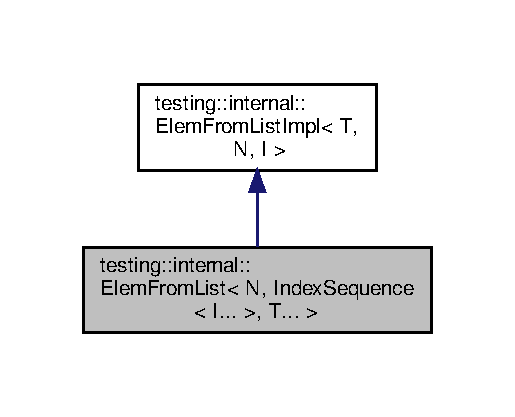
\includegraphics[width=247pt]{structtesting_1_1internal_1_1ElemFromList_3_01N_00_01IndexSequence_3_01I_8_8_8_01_4_00_01T_8_8_8_01_4__inherit__graph}
\end{center}
\end{figure}


Collaboration diagram for testing\+:\+:internal\+:\+:Elem\+From\+List$<$ N, Index\+Sequence$<$ I... $>$, T... $>$\+:\nopagebreak
\begin{figure}[H]
\begin{center}
\leavevmode
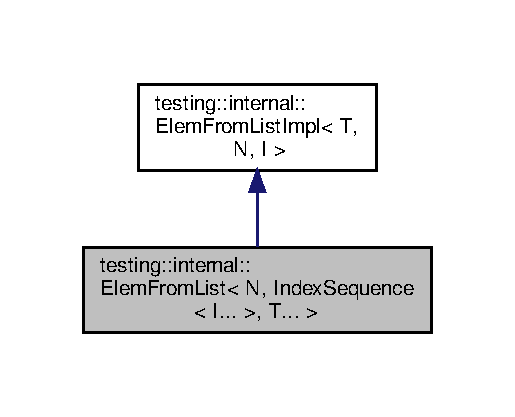
\includegraphics[width=247pt]{structtesting_1_1internal_1_1ElemFromList_3_01N_00_01IndexSequence_3_01I_8_8_8_01_4_00_01T_8_8_8_01_4__coll__graph}
\end{center}
\end{figure}


The documentation for this struct was generated from the following file\+:\begin{DoxyCompactItemize}
\item 
tests/googletest/include/gtest/internal/\hyperlink{gtest-internal_8h}{gtest-\/internal.\+h}\end{DoxyCompactItemize}

\hypertarget{structtesting_1_1internal_1_1ElemFromListImpl}{}\section{testing\+:\+:internal\+:\+:Elem\+From\+List\+Impl$<$ T, size\+\_\+t, size\+\_\+t $>$ Struct Template Reference}
\label{structtesting_1_1internal_1_1ElemFromListImpl}\index{testing\+::internal\+::\+Elem\+From\+List\+Impl$<$ T, size\+\_\+t, size\+\_\+t $>$@{testing\+::internal\+::\+Elem\+From\+List\+Impl$<$ T, size\+\_\+t, size\+\_\+t $>$}}


{\ttfamily \#include $<$gtest-\/internal.\+h$>$}



The documentation for this struct was generated from the following file\+:\begin{DoxyCompactItemize}
\item 
tests/googletest/include/gtest/internal/\hyperlink{gtest-internal_8h}{gtest-\/internal.\+h}\end{DoxyCompactItemize}

\hypertarget{structtesting_1_1internal_1_1ElemFromListImpl_3_01T_00_01I_00_01I_01_4}{}\section{testing\+:\+:internal\+:\+:Elem\+From\+List\+Impl$<$ T, I, I $>$ Struct Template Reference}
\label{structtesting_1_1internal_1_1ElemFromListImpl_3_01T_00_01I_00_01I_01_4}\index{testing\+::internal\+::\+Elem\+From\+List\+Impl$<$ T, I, I $>$@{testing\+::internal\+::\+Elem\+From\+List\+Impl$<$ T, I, I $>$}}


{\ttfamily \#include $<$gtest-\/internal.\+h$>$}

\subsection*{Public Types}
\begin{DoxyCompactItemize}
\item 
using \hyperlink{structtesting_1_1internal_1_1ElemFromListImpl_3_01T_00_01I_00_01I_01_4_ab1552e339cc1ff1e0aa448d684ffaf39}{type} = T
\end{DoxyCompactItemize}


\subsection{Member Typedef Documentation}
\mbox{\Hypertarget{structtesting_1_1internal_1_1ElemFromListImpl_3_01T_00_01I_00_01I_01_4_ab1552e339cc1ff1e0aa448d684ffaf39}\label{structtesting_1_1internal_1_1ElemFromListImpl_3_01T_00_01I_00_01I_01_4_ab1552e339cc1ff1e0aa448d684ffaf39}} 
\index{testing\+::internal\+::\+Elem\+From\+List\+Impl$<$ T, I, I $>$@{testing\+::internal\+::\+Elem\+From\+List\+Impl$<$ T, I, I $>$}!type@{type}}
\index{type@{type}!testing\+::internal\+::\+Elem\+From\+List\+Impl$<$ T, I, I $>$@{testing\+::internal\+::\+Elem\+From\+List\+Impl$<$ T, I, I $>$}}
\subsubsection{\texorpdfstring{type}{type}}
{\footnotesize\ttfamily template$<$typename T , size\+\_\+t I$>$ \\
using \hyperlink{structtesting_1_1internal_1_1ElemFromListImpl}{testing\+::internal\+::\+Elem\+From\+List\+Impl}$<$ T, I, I $>$\+::\hyperlink{structtesting_1_1internal_1_1ElemFromListImpl_3_01T_00_01I_00_01I_01_4_ab1552e339cc1ff1e0aa448d684ffaf39}{type} =  T}



The documentation for this struct was generated from the following file\+:\begin{DoxyCompactItemize}
\item 
tests/googletest/include/gtest/internal/\hyperlink{gtest-internal_8h}{gtest-\/internal.\+h}\end{DoxyCompactItemize}

\hypertarget{classtesting_1_1EmptyTestEventListener}{}\section{testing\+:\+:Empty\+Test\+Event\+Listener Class Reference}
\label{classtesting_1_1EmptyTestEventListener}\index{testing\+::\+Empty\+Test\+Event\+Listener@{testing\+::\+Empty\+Test\+Event\+Listener}}


{\ttfamily \#include $<$gtest.\+h$>$}



Inheritance diagram for testing\+:\+:Empty\+Test\+Event\+Listener\+:\nopagebreak
\begin{figure}[H]
\begin{center}
\leavevmode
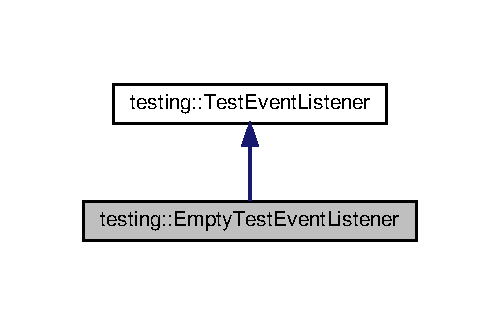
\includegraphics[width=240pt]{classtesting_1_1EmptyTestEventListener__inherit__graph}
\end{center}
\end{figure}


Collaboration diagram for testing\+:\+:Empty\+Test\+Event\+Listener\+:\nopagebreak
\begin{figure}[H]
\begin{center}
\leavevmode
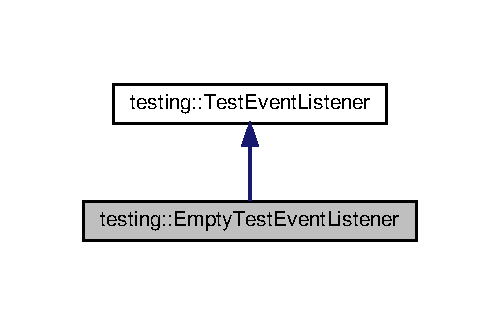
\includegraphics[width=240pt]{classtesting_1_1EmptyTestEventListener__coll__graph}
\end{center}
\end{figure}
\subsection*{Public Member Functions}
\begin{DoxyCompactItemize}
\item 
void \hyperlink{classtesting_1_1EmptyTestEventListener_ac3f5033fcd82080edb45f546ce9854fe}{On\+Test\+Program\+Start} (const \hyperlink{classtesting_1_1UnitTest}{Unit\+Test} \&) override
\item 
void \hyperlink{classtesting_1_1EmptyTestEventListener_a31edf103561e8b4d747656bc2d927661}{On\+Test\+Iteration\+Start} (const \hyperlink{classtesting_1_1UnitTest}{Unit\+Test} \&, int) override
\item 
void \hyperlink{classtesting_1_1EmptyTestEventListener_a6e498ae763ac8c1a46bd861e0b7ff3f5}{On\+Environments\+Set\+Up\+Start} (const \hyperlink{classtesting_1_1UnitTest}{Unit\+Test} \&) override
\item 
void \hyperlink{classtesting_1_1EmptyTestEventListener_a9b4e781c0b38065a55c2fd163724ba69}{On\+Environments\+Set\+Up\+End} (const \hyperlink{classtesting_1_1UnitTest}{Unit\+Test} \&) override
\item 
void \hyperlink{classtesting_1_1EmptyTestEventListener_a1e32e4bd4857822b6b50e6900aa5c651}{On\+Test\+Suite\+Start} (const \hyperlink{classtesting_1_1TestSuite}{Test\+Suite} \&) override
\item 
void \hyperlink{classtesting_1_1EmptyTestEventListener_a7f9a84967fde01000b7a56e9e84b6052}{On\+Test\+Case\+Start} (const Test\+Case \&) override
\item 
void \hyperlink{classtesting_1_1EmptyTestEventListener_a1d8c7f3f1f92826f668edae1bc5aadf4}{On\+Test\+Start} (const \hyperlink{classtesting_1_1TestInfo}{Test\+Info} \&) override
\item 
void \hyperlink{classtesting_1_1EmptyTestEventListener_ab95992f0a0b3741d59a24c3a7115fa60}{On\+Test\+Part\+Result} (const Test\+Part\+Result \&) override
\item 
void \hyperlink{classtesting_1_1EmptyTestEventListener_a709d7077c086c877d214231bc520ef90}{On\+Test\+End} (const \hyperlink{classtesting_1_1TestInfo}{Test\+Info} \&) override
\item 
void \hyperlink{classtesting_1_1EmptyTestEventListener_aefdb73682d290791461e186d864db718}{On\+Test\+Suite\+End} (const \hyperlink{classtesting_1_1TestSuite}{Test\+Suite} \&) override
\item 
void \hyperlink{classtesting_1_1EmptyTestEventListener_abe05cc74c1081ed51e2c84b73013299e}{On\+Test\+Case\+End} (const Test\+Case \&) override
\item 
void \hyperlink{classtesting_1_1EmptyTestEventListener_a320780451eac9178434b7c77d948ecbd}{On\+Environments\+Tear\+Down\+Start} (const \hyperlink{classtesting_1_1UnitTest}{Unit\+Test} \&) override
\item 
void \hyperlink{classtesting_1_1EmptyTestEventListener_ad9984052e82c3ae26395a2d9480326d2}{On\+Environments\+Tear\+Down\+End} (const \hyperlink{classtesting_1_1UnitTest}{Unit\+Test} \&) override
\item 
void \hyperlink{classtesting_1_1EmptyTestEventListener_aae9c5c61e476f0c421402fb1dde434d2}{On\+Test\+Iteration\+End} (const \hyperlink{classtesting_1_1UnitTest}{Unit\+Test} \&, int) override
\item 
void \hyperlink{classtesting_1_1EmptyTestEventListener_aaa9d683e8e0c850af67a0b92d785ddb9}{On\+Test\+Program\+End} (const \hyperlink{classtesting_1_1UnitTest}{Unit\+Test} \&) override
\end{DoxyCompactItemize}


\subsection{Member Function Documentation}
\mbox{\Hypertarget{classtesting_1_1EmptyTestEventListener_a9b4e781c0b38065a55c2fd163724ba69}\label{classtesting_1_1EmptyTestEventListener_a9b4e781c0b38065a55c2fd163724ba69}} 
\index{testing\+::\+Empty\+Test\+Event\+Listener@{testing\+::\+Empty\+Test\+Event\+Listener}!On\+Environments\+Set\+Up\+End@{On\+Environments\+Set\+Up\+End}}
\index{On\+Environments\+Set\+Up\+End@{On\+Environments\+Set\+Up\+End}!testing\+::\+Empty\+Test\+Event\+Listener@{testing\+::\+Empty\+Test\+Event\+Listener}}
\subsubsection{\texorpdfstring{On\+Environments\+Set\+Up\+End()}{OnEnvironmentsSetUpEnd()}}
{\footnotesize\ttfamily void testing\+::\+Empty\+Test\+Event\+Listener\+::\+On\+Environments\+Set\+Up\+End (\begin{DoxyParamCaption}\item[{const \hyperlink{classtesting_1_1UnitTest}{Unit\+Test} \&}]{ }\end{DoxyParamCaption})\hspace{0.3cm}{\ttfamily [inline]}, {\ttfamily [override]}, {\ttfamily [virtual]}}



Implements \hyperlink{classtesting_1_1TestEventListener_aaa1021d75f5dbf3f05c829c1cc520341}{testing\+::\+Test\+Event\+Listener}.

\mbox{\Hypertarget{classtesting_1_1EmptyTestEventListener_a6e498ae763ac8c1a46bd861e0b7ff3f5}\label{classtesting_1_1EmptyTestEventListener_a6e498ae763ac8c1a46bd861e0b7ff3f5}} 
\index{testing\+::\+Empty\+Test\+Event\+Listener@{testing\+::\+Empty\+Test\+Event\+Listener}!On\+Environments\+Set\+Up\+Start@{On\+Environments\+Set\+Up\+Start}}
\index{On\+Environments\+Set\+Up\+Start@{On\+Environments\+Set\+Up\+Start}!testing\+::\+Empty\+Test\+Event\+Listener@{testing\+::\+Empty\+Test\+Event\+Listener}}
\subsubsection{\texorpdfstring{On\+Environments\+Set\+Up\+Start()}{OnEnvironmentsSetUpStart()}}
{\footnotesize\ttfamily void testing\+::\+Empty\+Test\+Event\+Listener\+::\+On\+Environments\+Set\+Up\+Start (\begin{DoxyParamCaption}\item[{const \hyperlink{classtesting_1_1UnitTest}{Unit\+Test} \&}]{ }\end{DoxyParamCaption})\hspace{0.3cm}{\ttfamily [inline]}, {\ttfamily [override]}, {\ttfamily [virtual]}}



Implements \hyperlink{classtesting_1_1TestEventListener_aa6502e534919605be45f26a6daf9a40c}{testing\+::\+Test\+Event\+Listener}.

\mbox{\Hypertarget{classtesting_1_1EmptyTestEventListener_ad9984052e82c3ae26395a2d9480326d2}\label{classtesting_1_1EmptyTestEventListener_ad9984052e82c3ae26395a2d9480326d2}} 
\index{testing\+::\+Empty\+Test\+Event\+Listener@{testing\+::\+Empty\+Test\+Event\+Listener}!On\+Environments\+Tear\+Down\+End@{On\+Environments\+Tear\+Down\+End}}
\index{On\+Environments\+Tear\+Down\+End@{On\+Environments\+Tear\+Down\+End}!testing\+::\+Empty\+Test\+Event\+Listener@{testing\+::\+Empty\+Test\+Event\+Listener}}
\subsubsection{\texorpdfstring{On\+Environments\+Tear\+Down\+End()}{OnEnvironmentsTearDownEnd()}}
{\footnotesize\ttfamily void testing\+::\+Empty\+Test\+Event\+Listener\+::\+On\+Environments\+Tear\+Down\+End (\begin{DoxyParamCaption}\item[{const \hyperlink{classtesting_1_1UnitTest}{Unit\+Test} \&}]{ }\end{DoxyParamCaption})\hspace{0.3cm}{\ttfamily [inline]}, {\ttfamily [override]}, {\ttfamily [virtual]}}



Implements \hyperlink{classtesting_1_1TestEventListener_a9ea04fa7f447865ba76df35e12ba2092}{testing\+::\+Test\+Event\+Listener}.

\mbox{\Hypertarget{classtesting_1_1EmptyTestEventListener_a320780451eac9178434b7c77d948ecbd}\label{classtesting_1_1EmptyTestEventListener_a320780451eac9178434b7c77d948ecbd}} 
\index{testing\+::\+Empty\+Test\+Event\+Listener@{testing\+::\+Empty\+Test\+Event\+Listener}!On\+Environments\+Tear\+Down\+Start@{On\+Environments\+Tear\+Down\+Start}}
\index{On\+Environments\+Tear\+Down\+Start@{On\+Environments\+Tear\+Down\+Start}!testing\+::\+Empty\+Test\+Event\+Listener@{testing\+::\+Empty\+Test\+Event\+Listener}}
\subsubsection{\texorpdfstring{On\+Environments\+Tear\+Down\+Start()}{OnEnvironmentsTearDownStart()}}
{\footnotesize\ttfamily void testing\+::\+Empty\+Test\+Event\+Listener\+::\+On\+Environments\+Tear\+Down\+Start (\begin{DoxyParamCaption}\item[{const \hyperlink{classtesting_1_1UnitTest}{Unit\+Test} \&}]{ }\end{DoxyParamCaption})\hspace{0.3cm}{\ttfamily [inline]}, {\ttfamily [override]}, {\ttfamily [virtual]}}



Implements \hyperlink{classtesting_1_1TestEventListener_a468b5e6701bcb86cb2c956caadbba5e4}{testing\+::\+Test\+Event\+Listener}.

\mbox{\Hypertarget{classtesting_1_1EmptyTestEventListener_abe05cc74c1081ed51e2c84b73013299e}\label{classtesting_1_1EmptyTestEventListener_abe05cc74c1081ed51e2c84b73013299e}} 
\index{testing\+::\+Empty\+Test\+Event\+Listener@{testing\+::\+Empty\+Test\+Event\+Listener}!On\+Test\+Case\+End@{On\+Test\+Case\+End}}
\index{On\+Test\+Case\+End@{On\+Test\+Case\+End}!testing\+::\+Empty\+Test\+Event\+Listener@{testing\+::\+Empty\+Test\+Event\+Listener}}
\subsubsection{\texorpdfstring{On\+Test\+Case\+End()}{OnTestCaseEnd()}}
{\footnotesize\ttfamily void testing\+::\+Empty\+Test\+Event\+Listener\+::\+On\+Test\+Case\+End (\begin{DoxyParamCaption}\item[{const Test\+Case \&}]{ }\end{DoxyParamCaption})\hspace{0.3cm}{\ttfamily [inline]}, {\ttfamily [override]}, {\ttfamily [virtual]}}



Reimplemented from \hyperlink{classtesting_1_1TestEventListener_a6cada1572dde8010b94f6dd237ce52f4}{testing\+::\+Test\+Event\+Listener}.

\mbox{\Hypertarget{classtesting_1_1EmptyTestEventListener_a7f9a84967fde01000b7a56e9e84b6052}\label{classtesting_1_1EmptyTestEventListener_a7f9a84967fde01000b7a56e9e84b6052}} 
\index{testing\+::\+Empty\+Test\+Event\+Listener@{testing\+::\+Empty\+Test\+Event\+Listener}!On\+Test\+Case\+Start@{On\+Test\+Case\+Start}}
\index{On\+Test\+Case\+Start@{On\+Test\+Case\+Start}!testing\+::\+Empty\+Test\+Event\+Listener@{testing\+::\+Empty\+Test\+Event\+Listener}}
\subsubsection{\texorpdfstring{On\+Test\+Case\+Start()}{OnTestCaseStart()}}
{\footnotesize\ttfamily void testing\+::\+Empty\+Test\+Event\+Listener\+::\+On\+Test\+Case\+Start (\begin{DoxyParamCaption}\item[{const Test\+Case \&}]{ }\end{DoxyParamCaption})\hspace{0.3cm}{\ttfamily [inline]}, {\ttfamily [override]}, {\ttfamily [virtual]}}



Reimplemented from \hyperlink{classtesting_1_1TestEventListener_ac48628c9f78d3e10bff77c7366e9e780}{testing\+::\+Test\+Event\+Listener}.

\mbox{\Hypertarget{classtesting_1_1EmptyTestEventListener_a709d7077c086c877d214231bc520ef90}\label{classtesting_1_1EmptyTestEventListener_a709d7077c086c877d214231bc520ef90}} 
\index{testing\+::\+Empty\+Test\+Event\+Listener@{testing\+::\+Empty\+Test\+Event\+Listener}!On\+Test\+End@{On\+Test\+End}}
\index{On\+Test\+End@{On\+Test\+End}!testing\+::\+Empty\+Test\+Event\+Listener@{testing\+::\+Empty\+Test\+Event\+Listener}}
\subsubsection{\texorpdfstring{On\+Test\+End()}{OnTestEnd()}}
{\footnotesize\ttfamily void testing\+::\+Empty\+Test\+Event\+Listener\+::\+On\+Test\+End (\begin{DoxyParamCaption}\item[{const \hyperlink{classtesting_1_1TestInfo}{Test\+Info} \&}]{ }\end{DoxyParamCaption})\hspace{0.3cm}{\ttfamily [inline]}, {\ttfamily [override]}, {\ttfamily [virtual]}}



Implements \hyperlink{classtesting_1_1TestEventListener_abb1c44525ef038500608b5dc2f17099b}{testing\+::\+Test\+Event\+Listener}.

\mbox{\Hypertarget{classtesting_1_1EmptyTestEventListener_aae9c5c61e476f0c421402fb1dde434d2}\label{classtesting_1_1EmptyTestEventListener_aae9c5c61e476f0c421402fb1dde434d2}} 
\index{testing\+::\+Empty\+Test\+Event\+Listener@{testing\+::\+Empty\+Test\+Event\+Listener}!On\+Test\+Iteration\+End@{On\+Test\+Iteration\+End}}
\index{On\+Test\+Iteration\+End@{On\+Test\+Iteration\+End}!testing\+::\+Empty\+Test\+Event\+Listener@{testing\+::\+Empty\+Test\+Event\+Listener}}
\subsubsection{\texorpdfstring{On\+Test\+Iteration\+End()}{OnTestIterationEnd()}}
{\footnotesize\ttfamily void testing\+::\+Empty\+Test\+Event\+Listener\+::\+On\+Test\+Iteration\+End (\begin{DoxyParamCaption}\item[{const \hyperlink{classtesting_1_1UnitTest}{Unit\+Test} \&}]{,  }\item[{int}]{ }\end{DoxyParamCaption})\hspace{0.3cm}{\ttfamily [inline]}, {\ttfamily [override]}, {\ttfamily [virtual]}}



Implements \hyperlink{classtesting_1_1TestEventListener_a550fdb3e55726e4cefa09f5697941425}{testing\+::\+Test\+Event\+Listener}.

\mbox{\Hypertarget{classtesting_1_1EmptyTestEventListener_a31edf103561e8b4d747656bc2d927661}\label{classtesting_1_1EmptyTestEventListener_a31edf103561e8b4d747656bc2d927661}} 
\index{testing\+::\+Empty\+Test\+Event\+Listener@{testing\+::\+Empty\+Test\+Event\+Listener}!On\+Test\+Iteration\+Start@{On\+Test\+Iteration\+Start}}
\index{On\+Test\+Iteration\+Start@{On\+Test\+Iteration\+Start}!testing\+::\+Empty\+Test\+Event\+Listener@{testing\+::\+Empty\+Test\+Event\+Listener}}
\subsubsection{\texorpdfstring{On\+Test\+Iteration\+Start()}{OnTestIterationStart()}}
{\footnotesize\ttfamily void testing\+::\+Empty\+Test\+Event\+Listener\+::\+On\+Test\+Iteration\+Start (\begin{DoxyParamCaption}\item[{const \hyperlink{classtesting_1_1UnitTest}{Unit\+Test} \&}]{,  }\item[{int}]{ }\end{DoxyParamCaption})\hspace{0.3cm}{\ttfamily [inline]}, {\ttfamily [override]}, {\ttfamily [virtual]}}



Implements \hyperlink{classtesting_1_1TestEventListener_a60cc09b7907cb329d152eb5e7133bdeb}{testing\+::\+Test\+Event\+Listener}.

\mbox{\Hypertarget{classtesting_1_1EmptyTestEventListener_ab95992f0a0b3741d59a24c3a7115fa60}\label{classtesting_1_1EmptyTestEventListener_ab95992f0a0b3741d59a24c3a7115fa60}} 
\index{testing\+::\+Empty\+Test\+Event\+Listener@{testing\+::\+Empty\+Test\+Event\+Listener}!On\+Test\+Part\+Result@{On\+Test\+Part\+Result}}
\index{On\+Test\+Part\+Result@{On\+Test\+Part\+Result}!testing\+::\+Empty\+Test\+Event\+Listener@{testing\+::\+Empty\+Test\+Event\+Listener}}
\subsubsection{\texorpdfstring{On\+Test\+Part\+Result()}{OnTestPartResult()}}
{\footnotesize\ttfamily void testing\+::\+Empty\+Test\+Event\+Listener\+::\+On\+Test\+Part\+Result (\begin{DoxyParamCaption}\item[{const Test\+Part\+Result \&}]{ }\end{DoxyParamCaption})\hspace{0.3cm}{\ttfamily [inline]}, {\ttfamily [override]}, {\ttfamily [virtual]}}



Implements \hyperlink{classtesting_1_1TestEventListener_a054f8705c883fa120b91473aff38f2ee}{testing\+::\+Test\+Event\+Listener}.

\mbox{\Hypertarget{classtesting_1_1EmptyTestEventListener_aaa9d683e8e0c850af67a0b92d785ddb9}\label{classtesting_1_1EmptyTestEventListener_aaa9d683e8e0c850af67a0b92d785ddb9}} 
\index{testing\+::\+Empty\+Test\+Event\+Listener@{testing\+::\+Empty\+Test\+Event\+Listener}!On\+Test\+Program\+End@{On\+Test\+Program\+End}}
\index{On\+Test\+Program\+End@{On\+Test\+Program\+End}!testing\+::\+Empty\+Test\+Event\+Listener@{testing\+::\+Empty\+Test\+Event\+Listener}}
\subsubsection{\texorpdfstring{On\+Test\+Program\+End()}{OnTestProgramEnd()}}
{\footnotesize\ttfamily void testing\+::\+Empty\+Test\+Event\+Listener\+::\+On\+Test\+Program\+End (\begin{DoxyParamCaption}\item[{const \hyperlink{classtesting_1_1UnitTest}{Unit\+Test} \&}]{ }\end{DoxyParamCaption})\hspace{0.3cm}{\ttfamily [inline]}, {\ttfamily [override]}, {\ttfamily [virtual]}}



Implements \hyperlink{classtesting_1_1TestEventListener_ad15b6246d94c268e233487a86463ef3d}{testing\+::\+Test\+Event\+Listener}.

\mbox{\Hypertarget{classtesting_1_1EmptyTestEventListener_ac3f5033fcd82080edb45f546ce9854fe}\label{classtesting_1_1EmptyTestEventListener_ac3f5033fcd82080edb45f546ce9854fe}} 
\index{testing\+::\+Empty\+Test\+Event\+Listener@{testing\+::\+Empty\+Test\+Event\+Listener}!On\+Test\+Program\+Start@{On\+Test\+Program\+Start}}
\index{On\+Test\+Program\+Start@{On\+Test\+Program\+Start}!testing\+::\+Empty\+Test\+Event\+Listener@{testing\+::\+Empty\+Test\+Event\+Listener}}
\subsubsection{\texorpdfstring{On\+Test\+Program\+Start()}{OnTestProgramStart()}}
{\footnotesize\ttfamily void testing\+::\+Empty\+Test\+Event\+Listener\+::\+On\+Test\+Program\+Start (\begin{DoxyParamCaption}\item[{const \hyperlink{classtesting_1_1UnitTest}{Unit\+Test} \&}]{ }\end{DoxyParamCaption})\hspace{0.3cm}{\ttfamily [inline]}, {\ttfamily [override]}, {\ttfamily [virtual]}}



Implements \hyperlink{classtesting_1_1TestEventListener_a5f6c84f39851e8a603a2d2e10063816b}{testing\+::\+Test\+Event\+Listener}.

\mbox{\Hypertarget{classtesting_1_1EmptyTestEventListener_a1d8c7f3f1f92826f668edae1bc5aadf4}\label{classtesting_1_1EmptyTestEventListener_a1d8c7f3f1f92826f668edae1bc5aadf4}} 
\index{testing\+::\+Empty\+Test\+Event\+Listener@{testing\+::\+Empty\+Test\+Event\+Listener}!On\+Test\+Start@{On\+Test\+Start}}
\index{On\+Test\+Start@{On\+Test\+Start}!testing\+::\+Empty\+Test\+Event\+Listener@{testing\+::\+Empty\+Test\+Event\+Listener}}
\subsubsection{\texorpdfstring{On\+Test\+Start()}{OnTestStart()}}
{\footnotesize\ttfamily void testing\+::\+Empty\+Test\+Event\+Listener\+::\+On\+Test\+Start (\begin{DoxyParamCaption}\item[{const \hyperlink{classtesting_1_1TestInfo}{Test\+Info} \&}]{ }\end{DoxyParamCaption})\hspace{0.3cm}{\ttfamily [inline]}, {\ttfamily [override]}, {\ttfamily [virtual]}}



Implements \hyperlink{classtesting_1_1TestEventListener_ab4f6a0ca16ae75daf385b3b5914e1048}{testing\+::\+Test\+Event\+Listener}.

\mbox{\Hypertarget{classtesting_1_1EmptyTestEventListener_aefdb73682d290791461e186d864db718}\label{classtesting_1_1EmptyTestEventListener_aefdb73682d290791461e186d864db718}} 
\index{testing\+::\+Empty\+Test\+Event\+Listener@{testing\+::\+Empty\+Test\+Event\+Listener}!On\+Test\+Suite\+End@{On\+Test\+Suite\+End}}
\index{On\+Test\+Suite\+End@{On\+Test\+Suite\+End}!testing\+::\+Empty\+Test\+Event\+Listener@{testing\+::\+Empty\+Test\+Event\+Listener}}
\subsubsection{\texorpdfstring{On\+Test\+Suite\+End()}{OnTestSuiteEnd()}}
{\footnotesize\ttfamily void testing\+::\+Empty\+Test\+Event\+Listener\+::\+On\+Test\+Suite\+End (\begin{DoxyParamCaption}\item[{const \hyperlink{classtesting_1_1TestSuite}{Test\+Suite} \&}]{ }\end{DoxyParamCaption})\hspace{0.3cm}{\ttfamily [inline]}, {\ttfamily [override]}, {\ttfamily [virtual]}}



Reimplemented from \hyperlink{classtesting_1_1TestEventListener_a8962caad5d2522c9160c794074a662ee}{testing\+::\+Test\+Event\+Listener}.

\mbox{\Hypertarget{classtesting_1_1EmptyTestEventListener_a1e32e4bd4857822b6b50e6900aa5c651}\label{classtesting_1_1EmptyTestEventListener_a1e32e4bd4857822b6b50e6900aa5c651}} 
\index{testing\+::\+Empty\+Test\+Event\+Listener@{testing\+::\+Empty\+Test\+Event\+Listener}!On\+Test\+Suite\+Start@{On\+Test\+Suite\+Start}}
\index{On\+Test\+Suite\+Start@{On\+Test\+Suite\+Start}!testing\+::\+Empty\+Test\+Event\+Listener@{testing\+::\+Empty\+Test\+Event\+Listener}}
\subsubsection{\texorpdfstring{On\+Test\+Suite\+Start()}{OnTestSuiteStart()}}
{\footnotesize\ttfamily void testing\+::\+Empty\+Test\+Event\+Listener\+::\+On\+Test\+Suite\+Start (\begin{DoxyParamCaption}\item[{const \hyperlink{classtesting_1_1TestSuite}{Test\+Suite} \&}]{ }\end{DoxyParamCaption})\hspace{0.3cm}{\ttfamily [inline]}, {\ttfamily [override]}, {\ttfamily [virtual]}}



Reimplemented from \hyperlink{classtesting_1_1TestEventListener_a2726cc70dfda861f109355f1d9f09dfe}{testing\+::\+Test\+Event\+Listener}.



The documentation for this class was generated from the following file\+:\begin{DoxyCompactItemize}
\item 
tests/googletest/include/gtest/\hyperlink{gtest_8h}{gtest.\+h}\end{DoxyCompactItemize}

\hypertarget{structtesting_1_1internal_1_1EnableIf}{}\section{testing\+:\+:internal\+:\+:Enable\+If$<$ bool $>$ Struct Template Reference}
\label{structtesting_1_1internal_1_1EnableIf}\index{testing\+::internal\+::\+Enable\+If$<$ bool $>$@{testing\+::internal\+::\+Enable\+If$<$ bool $>$}}


{\ttfamily \#include $<$gtest-\/internal.\+h$>$}



The documentation for this struct was generated from the following file\+:\begin{DoxyCompactItemize}
\item 
tests/googletest/include/gtest/internal/\hyperlink{gtest-internal_8h}{gtest-\/internal.\+h}\end{DoxyCompactItemize}

\hypertarget{structtesting_1_1internal_1_1EnableIf_3_01true_01_4}{}\section{testing\+:\+:internal\+:\+:Enable\+If$<$ true $>$ Struct Template Reference}
\label{structtesting_1_1internal_1_1EnableIf_3_01true_01_4}\index{testing\+::internal\+::\+Enable\+If$<$ true $>$@{testing\+::internal\+::\+Enable\+If$<$ true $>$}}


{\ttfamily \#include $<$gtest-\/internal.\+h$>$}

\subsection*{Public Types}
\begin{DoxyCompactItemize}
\item 
typedef void \hyperlink{structtesting_1_1internal_1_1EnableIf_3_01true_01_4_a9398d803f1fdd99ff41823746f6299ff}{type}
\end{DoxyCompactItemize}


\subsection{Member Typedef Documentation}
\mbox{\Hypertarget{structtesting_1_1internal_1_1EnableIf_3_01true_01_4_a9398d803f1fdd99ff41823746f6299ff}\label{structtesting_1_1internal_1_1EnableIf_3_01true_01_4_a9398d803f1fdd99ff41823746f6299ff}} 
\index{testing\+::internal\+::\+Enable\+If$<$ true $>$@{testing\+::internal\+::\+Enable\+If$<$ true $>$}!type@{type}}
\index{type@{type}!testing\+::internal\+::\+Enable\+If$<$ true $>$@{testing\+::internal\+::\+Enable\+If$<$ true $>$}}
\subsubsection{\texorpdfstring{type}{type}}
{\footnotesize\ttfamily typedef void \hyperlink{structtesting_1_1internal_1_1EnableIf}{testing\+::internal\+::\+Enable\+If}$<$ true $>$\+::\hyperlink{structtesting_1_1internal_1_1EnableIf_3_01true_01_4_a9398d803f1fdd99ff41823746f6299ff}{type}}



The documentation for this struct was generated from the following file\+:\begin{DoxyCompactItemize}
\item 
tests/googletest/include/gtest/internal/\hyperlink{gtest-internal_8h}{gtest-\/internal.\+h}\end{DoxyCompactItemize}

\hypertarget{classtesting_1_1Environment}{}\section{testing\+:\+:Environment Class Reference}
\label{classtesting_1_1Environment}\index{testing\+::\+Environment@{testing\+::\+Environment}}


{\ttfamily \#include $<$gtest.\+h$>$}

\subsection*{Classes}
\begin{DoxyCompactItemize}
\item 
struct \hyperlink{structtesting_1_1Environment_1_1Setup__should__be__spelled__SetUp}{Setup\+\_\+should\+\_\+be\+\_\+spelled\+\_\+\+Set\+Up}
\end{DoxyCompactItemize}
\subsection*{Public Member Functions}
\begin{DoxyCompactItemize}
\item 
virtual \hyperlink{classtesting_1_1Environment_a0e41c320362576d752cd1f44cabd57d4}{$\sim$\+Environment} ()
\item 
virtual void \hyperlink{classtesting_1_1Environment_a1bf8cafaa9d4eba9feb98655ee434eb3}{Set\+Up} ()
\item 
virtual void \hyperlink{classtesting_1_1Environment_a039bdaa705c46b9b88234cf4d3bb6254}{Tear\+Down} ()
\end{DoxyCompactItemize}
\subsection*{Private Member Functions}
\begin{DoxyCompactItemize}
\item 
virtual \hyperlink{structtesting_1_1Environment_1_1Setup__should__be__spelled__SetUp}{Setup\+\_\+should\+\_\+be\+\_\+spelled\+\_\+\+Set\+Up} $\ast$ \hyperlink{classtesting_1_1Environment_a6096a69b03f6eb727a69a39f854cc87b}{Setup} ()
\end{DoxyCompactItemize}


\subsection{Constructor \& Destructor Documentation}
\mbox{\Hypertarget{classtesting_1_1Environment_a0e41c320362576d752cd1f44cabd57d4}\label{classtesting_1_1Environment_a0e41c320362576d752cd1f44cabd57d4}} 
\index{testing\+::\+Environment@{testing\+::\+Environment}!````~Environment@{$\sim$\+Environment}}
\index{````~Environment@{$\sim$\+Environment}!testing\+::\+Environment@{testing\+::\+Environment}}
\subsubsection{\texorpdfstring{$\sim$\+Environment()}{~Environment()}}
{\footnotesize\ttfamily virtual testing\+::\+Environment\+::$\sim$\+Environment (\begin{DoxyParamCaption}{ }\end{DoxyParamCaption})\hspace{0.3cm}{\ttfamily [inline]}, {\ttfamily [virtual]}}



\subsection{Member Function Documentation}
\mbox{\Hypertarget{classtesting_1_1Environment_a1bf8cafaa9d4eba9feb98655ee434eb3}\label{classtesting_1_1Environment_a1bf8cafaa9d4eba9feb98655ee434eb3}} 
\index{testing\+::\+Environment@{testing\+::\+Environment}!Set\+Up@{Set\+Up}}
\index{Set\+Up@{Set\+Up}!testing\+::\+Environment@{testing\+::\+Environment}}
\subsubsection{\texorpdfstring{Set\+Up()}{SetUp()}}
{\footnotesize\ttfamily virtual void testing\+::\+Environment\+::\+Set\+Up (\begin{DoxyParamCaption}{ }\end{DoxyParamCaption})\hspace{0.3cm}{\ttfamily [inline]}, {\ttfamily [virtual]}}

\mbox{\Hypertarget{classtesting_1_1Environment_a6096a69b03f6eb727a69a39f854cc87b}\label{classtesting_1_1Environment_a6096a69b03f6eb727a69a39f854cc87b}} 
\index{testing\+::\+Environment@{testing\+::\+Environment}!Setup@{Setup}}
\index{Setup@{Setup}!testing\+::\+Environment@{testing\+::\+Environment}}
\subsubsection{\texorpdfstring{Setup()}{Setup()}}
{\footnotesize\ttfamily virtual \hyperlink{structtesting_1_1Environment_1_1Setup__should__be__spelled__SetUp}{Setup\+\_\+should\+\_\+be\+\_\+spelled\+\_\+\+Set\+Up}$\ast$ testing\+::\+Environment\+::\+Setup (\begin{DoxyParamCaption}{ }\end{DoxyParamCaption})\hspace{0.3cm}{\ttfamily [inline]}, {\ttfamily [private]}, {\ttfamily [virtual]}}

\mbox{\Hypertarget{classtesting_1_1Environment_a039bdaa705c46b9b88234cf4d3bb6254}\label{classtesting_1_1Environment_a039bdaa705c46b9b88234cf4d3bb6254}} 
\index{testing\+::\+Environment@{testing\+::\+Environment}!Tear\+Down@{Tear\+Down}}
\index{Tear\+Down@{Tear\+Down}!testing\+::\+Environment@{testing\+::\+Environment}}
\subsubsection{\texorpdfstring{Tear\+Down()}{TearDown()}}
{\footnotesize\ttfamily virtual void testing\+::\+Environment\+::\+Tear\+Down (\begin{DoxyParamCaption}{ }\end{DoxyParamCaption})\hspace{0.3cm}{\ttfamily [inline]}, {\ttfamily [virtual]}}



The documentation for this class was generated from the following file\+:\begin{DoxyCompactItemize}
\item 
tests/googletest/include/gtest/\hyperlink{gtest_8h}{gtest.\+h}\end{DoxyCompactItemize}

\hypertarget{classtesting_1_1internal_1_1EqHelper}{}\section{testing\+:\+:internal\+:\+:Eq\+Helper Class Reference}
\label{classtesting_1_1internal_1_1EqHelper}\index{testing\+::internal\+::\+Eq\+Helper@{testing\+::internal\+::\+Eq\+Helper}}


{\ttfamily \#include $<$gtest.\+h$>$}

\subsection*{Static Public Member Functions}
\begin{DoxyCompactItemize}
\item 
{\footnotesize template$<$typename T1 , typename T2 , typename std\+::enable\+\_\+if$<$!std\+::is\+\_\+integral$<$ T1 $>$\+::value$\vert$$\vert$!std\+::is\+\_\+pointer$<$ T2 $>$\+::value $>$\+::type $\ast$  = nullptr$>$ }\\static Assertion\+Result \hyperlink{classtesting_1_1internal_1_1EqHelper_aa5ee2dafddce2496d73ba13fd34bb981}{Compare} (const char $\ast$lhs\+\_\+expression, const char $\ast$rhs\+\_\+expression, const T1 \&lhs, const T2 \&rhs)
\item 
static Assertion\+Result \hyperlink{classtesting_1_1internal_1_1EqHelper_af7e402f6e00be1486d0f102e9f1bc931}{Compare} (const char $\ast$lhs\+\_\+expression, const char $\ast$rhs\+\_\+expression, \hyperlink{namespacetesting_1_1internal_a05c6bd9ede5ccdf25191a590d610dcc6}{Biggest\+Int} lhs, \hyperlink{namespacetesting_1_1internal_a05c6bd9ede5ccdf25191a590d610dcc6}{Biggest\+Int} rhs)
\item 
{\footnotesize template$<$typename T $>$ }\\static Assertion\+Result \hyperlink{classtesting_1_1internal_1_1EqHelper_af5cac2c28545dfa0688849e205f54bec}{Compare} (const char $\ast$lhs\+\_\+expression, const char $\ast$rhs\+\_\+expression, std\+::nullptr\+\_\+t, T $\ast$rhs)
\end{DoxyCompactItemize}


\subsection{Member Function Documentation}
\mbox{\Hypertarget{classtesting_1_1internal_1_1EqHelper_aa5ee2dafddce2496d73ba13fd34bb981}\label{classtesting_1_1internal_1_1EqHelper_aa5ee2dafddce2496d73ba13fd34bb981}} 
\index{testing\+::internal\+::\+Eq\+Helper@{testing\+::internal\+::\+Eq\+Helper}!Compare@{Compare}}
\index{Compare@{Compare}!testing\+::internal\+::\+Eq\+Helper@{testing\+::internal\+::\+Eq\+Helper}}
\subsubsection{\texorpdfstring{Compare()}{Compare()}\hspace{0.1cm}{\footnotesize\ttfamily [1/3]}}
{\footnotesize\ttfamily template$<$typename T1 , typename T2 , typename std\+::enable\+\_\+if$<$!std\+::is\+\_\+integral$<$ T1 $>$\+::value$\vert$$\vert$!std\+::is\+\_\+pointer$<$ T2 $>$\+::value $>$\+::type $\ast$  = nullptr$>$ \\
static Assertion\+Result testing\+::internal\+::\+Eq\+Helper\+::\+Compare (\begin{DoxyParamCaption}\item[{const char $\ast$}]{lhs\+\_\+expression,  }\item[{const char $\ast$}]{rhs\+\_\+expression,  }\item[{const T1 \&}]{lhs,  }\item[{const T2 \&}]{rhs }\end{DoxyParamCaption})\hspace{0.3cm}{\ttfamily [inline]}, {\ttfamily [static]}}

\mbox{\Hypertarget{classtesting_1_1internal_1_1EqHelper_af7e402f6e00be1486d0f102e9f1bc931}\label{classtesting_1_1internal_1_1EqHelper_af7e402f6e00be1486d0f102e9f1bc931}} 
\index{testing\+::internal\+::\+Eq\+Helper@{testing\+::internal\+::\+Eq\+Helper}!Compare@{Compare}}
\index{Compare@{Compare}!testing\+::internal\+::\+Eq\+Helper@{testing\+::internal\+::\+Eq\+Helper}}
\subsubsection{\texorpdfstring{Compare()}{Compare()}\hspace{0.1cm}{\footnotesize\ttfamily [2/3]}}
{\footnotesize\ttfamily static Assertion\+Result testing\+::internal\+::\+Eq\+Helper\+::\+Compare (\begin{DoxyParamCaption}\item[{const char $\ast$}]{lhs\+\_\+expression,  }\item[{const char $\ast$}]{rhs\+\_\+expression,  }\item[{\hyperlink{namespacetesting_1_1internal_a05c6bd9ede5ccdf25191a590d610dcc6}{Biggest\+Int}}]{lhs,  }\item[{\hyperlink{namespacetesting_1_1internal_a05c6bd9ede5ccdf25191a590d610dcc6}{Biggest\+Int}}]{rhs }\end{DoxyParamCaption})\hspace{0.3cm}{\ttfamily [inline]}, {\ttfamily [static]}}

\mbox{\Hypertarget{classtesting_1_1internal_1_1EqHelper_af5cac2c28545dfa0688849e205f54bec}\label{classtesting_1_1internal_1_1EqHelper_af5cac2c28545dfa0688849e205f54bec}} 
\index{testing\+::internal\+::\+Eq\+Helper@{testing\+::internal\+::\+Eq\+Helper}!Compare@{Compare}}
\index{Compare@{Compare}!testing\+::internal\+::\+Eq\+Helper@{testing\+::internal\+::\+Eq\+Helper}}
\subsubsection{\texorpdfstring{Compare()}{Compare()}\hspace{0.1cm}{\footnotesize\ttfamily [3/3]}}
{\footnotesize\ttfamily template$<$typename T $>$ \\
static Assertion\+Result testing\+::internal\+::\+Eq\+Helper\+::\+Compare (\begin{DoxyParamCaption}\item[{const char $\ast$}]{lhs\+\_\+expression,  }\item[{const char $\ast$}]{rhs\+\_\+expression,  }\item[{std\+::nullptr\+\_\+t}]{,  }\item[{T $\ast$}]{rhs }\end{DoxyParamCaption})\hspace{0.3cm}{\ttfamily [inline]}, {\ttfamily [static]}}



The documentation for this class was generated from the following file\+:\begin{DoxyCompactItemize}
\item 
tests/googletest/include/gtest/\hyperlink{gtest_8h}{gtest.\+h}\end{DoxyCompactItemize}

\hypertarget{classExternalInstantiationTest}{}\section{External\+Instantiation\+Test Class Reference}
\label{classExternalInstantiationTest}\index{External\+Instantiation\+Test@{External\+Instantiation\+Test}}


{\ttfamily \#include $<$googletest-\/param-\/test-\/test.\+h$>$}



Inheritance diagram for External\+Instantiation\+Test\+:\nopagebreak
\begin{figure}[H]
\begin{center}
\leavevmode
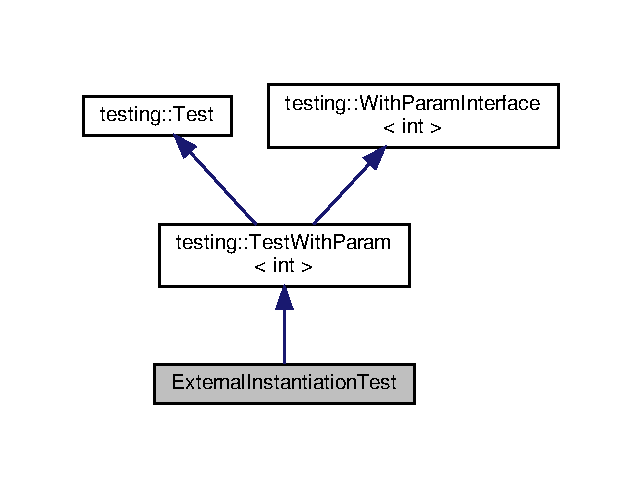
\includegraphics[width=308pt]{classExternalInstantiationTest__inherit__graph}
\end{center}
\end{figure}


Collaboration diagram for External\+Instantiation\+Test\+:\nopagebreak
\begin{figure}[H]
\begin{center}
\leavevmode
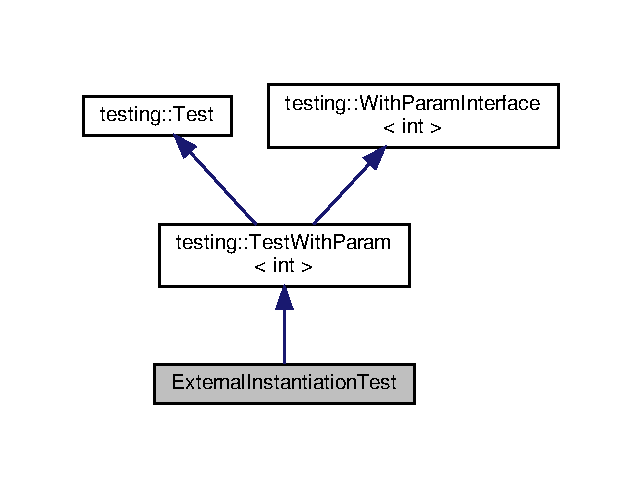
\includegraphics[width=308pt]{classExternalInstantiationTest__coll__graph}
\end{center}
\end{figure}
\subsection*{Additional Inherited Members}


The documentation for this class was generated from the following file\+:\begin{DoxyCompactItemize}
\item 
tests/googletest/test/\hyperlink{googletest-param-test-test_8h}{googletest-\/param-\/test-\/test.\+h}\end{DoxyCompactItemize}

\hypertarget{structtesting_1_1internal_1_1faketype}{}\section{testing\+:\+:internal\+:\+:faketype Struct Reference}
\label{structtesting_1_1internal_1_1faketype}\index{testing\+::internal\+::faketype@{testing\+::internal\+::faketype}}


{\ttfamily \#include $<$gtest.\+h$>$}



The documentation for this struct was generated from the following file\+:\begin{DoxyCompactItemize}
\item 
tests/googletest/include/gtest/\hyperlink{gtest_8h}{gtest.\+h}\end{DoxyCompactItemize}

\hypertarget{classtesting_1_1internal_1_1FlatTuple}{}\section{testing\+:\+:internal\+:\+:Flat\+Tuple$<$ T $>$ Class Template Reference}
\label{classtesting_1_1internal_1_1FlatTuple}\index{testing\+::internal\+::\+Flat\+Tuple$<$ T $>$@{testing\+::internal\+::\+Flat\+Tuple$<$ T $>$}}


{\ttfamily \#include $<$gtest-\/internal.\+h$>$}



Inheritance diagram for testing\+:\+:internal\+:\+:Flat\+Tuple$<$ T $>$\+:\nopagebreak
\begin{figure}[H]
\begin{center}
\leavevmode
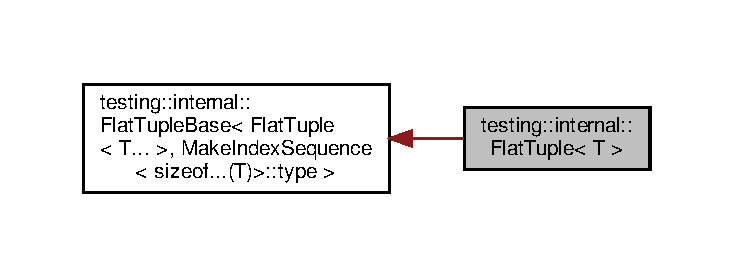
\includegraphics[width=350pt]{classtesting_1_1internal_1_1FlatTuple__inherit__graph}
\end{center}
\end{figure}


Collaboration diagram for testing\+:\+:internal\+:\+:Flat\+Tuple$<$ T $>$\+:\nopagebreak
\begin{figure}[H]
\begin{center}
\leavevmode
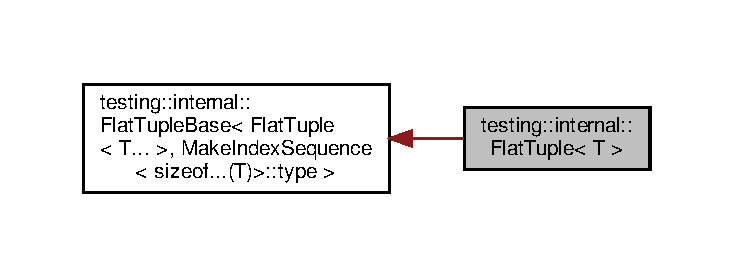
\includegraphics[width=350pt]{classtesting_1_1internal_1_1FlatTuple__coll__graph}
\end{center}
\end{figure}
\subsection*{Public Member Functions}
\begin{DoxyCompactItemize}
\item 
\hyperlink{classtesting_1_1internal_1_1FlatTuple_a056c58b5dd85f470ec5db1db9956c702}{Flat\+Tuple} ()=default
\item 
\hyperlink{classtesting_1_1internal_1_1FlatTuple_a611d01b9ff2437e4b9cfe3bbedc6d6ae}{Flat\+Tuple} (T... t)
\item 
{\footnotesize template$<$size\+\_\+t I$>$ }\\const \hyperlink{structtesting_1_1internal_1_1ElemFromList}{Elem\+From\+List}$<$ I, \hyperlink{classtesting_1_1internal_1_1FlatTuple_a004b42fc11ac1a85a9b1560fa83cdf77}{Indices}, T... $>$\+::type \& \hyperlink{classtesting_1_1internal_1_1FlatTuple_a9ea6508fa6413ceca5e38b8077c67938}{Get} () const
\item 
{\footnotesize template$<$size\+\_\+t I$>$ }\\\hyperlink{structtesting_1_1internal_1_1ElemFromList}{Elem\+From\+List}$<$ I, \hyperlink{classtesting_1_1internal_1_1FlatTuple_a004b42fc11ac1a85a9b1560fa83cdf77}{Indices}, T... $>$\+::type \& \hyperlink{classtesting_1_1internal_1_1FlatTuple_a48a13560f8963f727d81a7922e3b3e50}{Get} ()
\end{DoxyCompactItemize}
\subsection*{Private Types}
\begin{DoxyCompactItemize}
\item 
using \hyperlink{classtesting_1_1internal_1_1FlatTuple_a004b42fc11ac1a85a9b1560fa83cdf77}{Indices} = typename Flat\+Tuple\+::\+Flat\+Tuple\+Base\+::\+Indices
\end{DoxyCompactItemize}


\subsection{Member Typedef Documentation}
\mbox{\Hypertarget{classtesting_1_1internal_1_1FlatTuple_a004b42fc11ac1a85a9b1560fa83cdf77}\label{classtesting_1_1internal_1_1FlatTuple_a004b42fc11ac1a85a9b1560fa83cdf77}} 
\index{testing\+::internal\+::\+Flat\+Tuple@{testing\+::internal\+::\+Flat\+Tuple}!Indices@{Indices}}
\index{Indices@{Indices}!testing\+::internal\+::\+Flat\+Tuple@{testing\+::internal\+::\+Flat\+Tuple}}
\subsubsection{\texorpdfstring{Indices}{Indices}}
{\footnotesize\ttfamily template$<$typename... T$>$ \\
using \hyperlink{classtesting_1_1internal_1_1FlatTuple}{testing\+::internal\+::\+Flat\+Tuple}$<$ T $>$\+::\hyperlink{classtesting_1_1internal_1_1FlatTuple_a004b42fc11ac1a85a9b1560fa83cdf77}{Indices} =  typename Flat\+Tuple\+::\+Flat\+Tuple\+Base\+::\+Indices\hspace{0.3cm}{\ttfamily [private]}}



\subsection{Constructor \& Destructor Documentation}
\mbox{\Hypertarget{classtesting_1_1internal_1_1FlatTuple_a056c58b5dd85f470ec5db1db9956c702}\label{classtesting_1_1internal_1_1FlatTuple_a056c58b5dd85f470ec5db1db9956c702}} 
\index{testing\+::internal\+::\+Flat\+Tuple@{testing\+::internal\+::\+Flat\+Tuple}!Flat\+Tuple@{Flat\+Tuple}}
\index{Flat\+Tuple@{Flat\+Tuple}!testing\+::internal\+::\+Flat\+Tuple@{testing\+::internal\+::\+Flat\+Tuple}}
\subsubsection{\texorpdfstring{Flat\+Tuple()}{FlatTuple()}\hspace{0.1cm}{\footnotesize\ttfamily [1/2]}}
{\footnotesize\ttfamily template$<$typename... T$>$ \\
\hyperlink{classtesting_1_1internal_1_1FlatTuple}{testing\+::internal\+::\+Flat\+Tuple}$<$ T $>$\+::\hyperlink{classtesting_1_1internal_1_1FlatTuple}{Flat\+Tuple} (\begin{DoxyParamCaption}{ }\end{DoxyParamCaption})\hspace{0.3cm}{\ttfamily [default]}}

\mbox{\Hypertarget{classtesting_1_1internal_1_1FlatTuple_a611d01b9ff2437e4b9cfe3bbedc6d6ae}\label{classtesting_1_1internal_1_1FlatTuple_a611d01b9ff2437e4b9cfe3bbedc6d6ae}} 
\index{testing\+::internal\+::\+Flat\+Tuple@{testing\+::internal\+::\+Flat\+Tuple}!Flat\+Tuple@{Flat\+Tuple}}
\index{Flat\+Tuple@{Flat\+Tuple}!testing\+::internal\+::\+Flat\+Tuple@{testing\+::internal\+::\+Flat\+Tuple}}
\subsubsection{\texorpdfstring{Flat\+Tuple()}{FlatTuple()}\hspace{0.1cm}{\footnotesize\ttfamily [2/2]}}
{\footnotesize\ttfamily template$<$typename... T$>$ \\
\hyperlink{classtesting_1_1internal_1_1FlatTuple}{testing\+::internal\+::\+Flat\+Tuple}$<$ T $>$\+::\hyperlink{classtesting_1_1internal_1_1FlatTuple}{Flat\+Tuple} (\begin{DoxyParamCaption}\item[{T...}]{t }\end{DoxyParamCaption})\hspace{0.3cm}{\ttfamily [inline]}, {\ttfamily [explicit]}}



\subsection{Member Function Documentation}
\mbox{\Hypertarget{classtesting_1_1internal_1_1FlatTuple_a9ea6508fa6413ceca5e38b8077c67938}\label{classtesting_1_1internal_1_1FlatTuple_a9ea6508fa6413ceca5e38b8077c67938}} 
\index{testing\+::internal\+::\+Flat\+Tuple@{testing\+::internal\+::\+Flat\+Tuple}!Get@{Get}}
\index{Get@{Get}!testing\+::internal\+::\+Flat\+Tuple@{testing\+::internal\+::\+Flat\+Tuple}}
\subsubsection{\texorpdfstring{Get()}{Get()}\hspace{0.1cm}{\footnotesize\ttfamily [1/2]}}
{\footnotesize\ttfamily template$<$typename... T$>$ \\
template$<$size\+\_\+t I$>$ \\
const \hyperlink{structtesting_1_1internal_1_1ElemFromList}{Elem\+From\+List}$<$I, \hyperlink{classtesting_1_1internal_1_1FlatTuple_a004b42fc11ac1a85a9b1560fa83cdf77}{Indices}, T...$>$\+::type\& \hyperlink{classtesting_1_1internal_1_1FlatTuple}{testing\+::internal\+::\+Flat\+Tuple}$<$ T $>$\+::Get (\begin{DoxyParamCaption}{ }\end{DoxyParamCaption}) const\hspace{0.3cm}{\ttfamily [inline]}}

\mbox{\Hypertarget{classtesting_1_1internal_1_1FlatTuple_a48a13560f8963f727d81a7922e3b3e50}\label{classtesting_1_1internal_1_1FlatTuple_a48a13560f8963f727d81a7922e3b3e50}} 
\index{testing\+::internal\+::\+Flat\+Tuple@{testing\+::internal\+::\+Flat\+Tuple}!Get@{Get}}
\index{Get@{Get}!testing\+::internal\+::\+Flat\+Tuple@{testing\+::internal\+::\+Flat\+Tuple}}
\subsubsection{\texorpdfstring{Get()}{Get()}\hspace{0.1cm}{\footnotesize\ttfamily [2/2]}}
{\footnotesize\ttfamily template$<$typename... T$>$ \\
template$<$size\+\_\+t I$>$ \\
\hyperlink{structtesting_1_1internal_1_1ElemFromList}{Elem\+From\+List}$<$I, \hyperlink{classtesting_1_1internal_1_1FlatTuple_a004b42fc11ac1a85a9b1560fa83cdf77}{Indices}, T...$>$\+::type\& \hyperlink{classtesting_1_1internal_1_1FlatTuple}{testing\+::internal\+::\+Flat\+Tuple}$<$ T $>$\+::Get (\begin{DoxyParamCaption}{ }\end{DoxyParamCaption})\hspace{0.3cm}{\ttfamily [inline]}}



The documentation for this class was generated from the following file\+:\begin{DoxyCompactItemize}
\item 
tests/googletest/include/gtest/internal/\hyperlink{gtest-internal_8h}{gtest-\/internal.\+h}\end{DoxyCompactItemize}

\hypertarget{structtesting_1_1internal_1_1FlatTupleBase}{}\section{testing\+:\+:internal\+:\+:Flat\+Tuple\+Base$<$ Derived, Idx $>$ Struct Template Reference}
\label{structtesting_1_1internal_1_1FlatTupleBase}\index{testing\+::internal\+::\+Flat\+Tuple\+Base$<$ Derived, Idx $>$@{testing\+::internal\+::\+Flat\+Tuple\+Base$<$ Derived, Idx $>$}}


{\ttfamily \#include $<$gtest-\/internal.\+h$>$}



The documentation for this struct was generated from the following file\+:\begin{DoxyCompactItemize}
\item 
tests/googletest/include/gtest/internal/\hyperlink{gtest-internal_8h}{gtest-\/internal.\+h}\end{DoxyCompactItemize}

\hypertarget{structtesting_1_1internal_1_1FlatTupleBase_3_01FlatTuple_3_01T_8_8_8_01_4_00_01IndexSequence_3_01Idx_8_8_8_01_4_01_4}{}\section{testing\+:\+:internal\+:\+:Flat\+Tuple\+Base$<$ Flat\+Tuple$<$ T... $>$, Index\+Sequence$<$ Idx... $>$ $>$ Struct Template Reference}
\label{structtesting_1_1internal_1_1FlatTupleBase_3_01FlatTuple_3_01T_8_8_8_01_4_00_01IndexSequence_3_01Idx_8_8_8_01_4_01_4}\index{testing\+::internal\+::\+Flat\+Tuple\+Base$<$ Flat\+Tuple$<$ T... $>$, Index\+Sequence$<$ Idx... $>$ $>$@{testing\+::internal\+::\+Flat\+Tuple\+Base$<$ Flat\+Tuple$<$ T... $>$, Index\+Sequence$<$ Idx... $>$ $>$}}


{\ttfamily \#include $<$gtest-\/internal.\+h$>$}



Inheritance diagram for testing\+:\+:internal\+:\+:Flat\+Tuple\+Base$<$ Flat\+Tuple$<$ T... $>$, Index\+Sequence$<$ Idx... $>$ $>$\+:\nopagebreak
\begin{figure}[H]
\begin{center}
\leavevmode
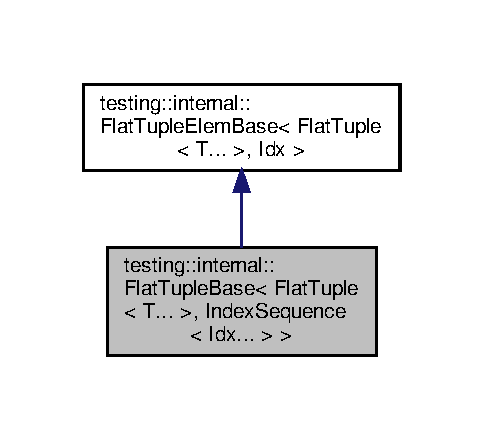
\includegraphics[width=232pt]{structtesting_1_1internal_1_1FlatTupleBase_3_01FlatTuple_3_01T_8_8_8_01_4_00_01IndexSequence_3_00431fb417381c8c3c9e075fb35152a07}
\end{center}
\end{figure}


Collaboration diagram for testing\+:\+:internal\+:\+:Flat\+Tuple\+Base$<$ Flat\+Tuple$<$ T... $>$, Index\+Sequence$<$ Idx... $>$ $>$\+:\nopagebreak
\begin{figure}[H]
\begin{center}
\leavevmode
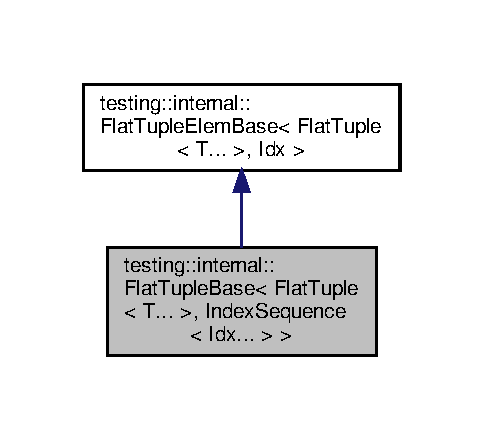
\includegraphics[width=232pt]{structtesting_1_1internal_1_1FlatTupleBase_3_01FlatTuple_3_01T_8_8_8_01_4_00_01IndexSequence_3_0db435676f5b40a729de5146d36fb9cc6}
\end{center}
\end{figure}
\subsection*{Public Types}
\begin{DoxyCompactItemize}
\item 
using \hyperlink{structtesting_1_1internal_1_1FlatTupleBase_3_01FlatTuple_3_01T_8_8_8_01_4_00_01IndexSequence_3_01Idx_8_8_8_01_4_01_4_ada1941ebde1ec1c844b72970e0ccb304}{Indices} = \hyperlink{structtesting_1_1internal_1_1IndexSequence}{Index\+Sequence}$<$ Idx... $>$
\end{DoxyCompactItemize}
\subsection*{Public Member Functions}
\begin{DoxyCompactItemize}
\item 
\hyperlink{structtesting_1_1internal_1_1FlatTupleBase_3_01FlatTuple_3_01T_8_8_8_01_4_00_01IndexSequence_3_01Idx_8_8_8_01_4_01_4_ae509b146e74176bceddc0d2f2d1cb0dc}{Flat\+Tuple\+Base} ()=default
\item 
\hyperlink{structtesting_1_1internal_1_1FlatTupleBase_3_01FlatTuple_3_01T_8_8_8_01_4_00_01IndexSequence_3_01Idx_8_8_8_01_4_01_4_ac515eec5c0647748bf8fa4ff553c706e}{Flat\+Tuple\+Base} (T... t)
\end{DoxyCompactItemize}


\subsection{Member Typedef Documentation}
\mbox{\Hypertarget{structtesting_1_1internal_1_1FlatTupleBase_3_01FlatTuple_3_01T_8_8_8_01_4_00_01IndexSequence_3_01Idx_8_8_8_01_4_01_4_ada1941ebde1ec1c844b72970e0ccb304}\label{structtesting_1_1internal_1_1FlatTupleBase_3_01FlatTuple_3_01T_8_8_8_01_4_00_01IndexSequence_3_01Idx_8_8_8_01_4_01_4_ada1941ebde1ec1c844b72970e0ccb304}} 
\index{testing\+::internal\+::\+Flat\+Tuple\+Base$<$ Flat\+Tuple$<$ T... $>$, Index\+Sequence$<$ Idx... $>$ $>$@{testing\+::internal\+::\+Flat\+Tuple\+Base$<$ Flat\+Tuple$<$ T... $>$, Index\+Sequence$<$ Idx... $>$ $>$}!Indices@{Indices}}
\index{Indices@{Indices}!testing\+::internal\+::\+Flat\+Tuple\+Base$<$ Flat\+Tuple$<$ T... $>$, Index\+Sequence$<$ Idx... $>$ $>$@{testing\+::internal\+::\+Flat\+Tuple\+Base$<$ Flat\+Tuple$<$ T... $>$, Index\+Sequence$<$ Idx... $>$ $>$}}
\subsubsection{\texorpdfstring{Indices}{Indices}}
{\footnotesize\ttfamily template$<$size\+\_\+t... Idx, typename... T$>$ \\
using \hyperlink{structtesting_1_1internal_1_1FlatTupleBase}{testing\+::internal\+::\+Flat\+Tuple\+Base}$<$ \hyperlink{classtesting_1_1internal_1_1FlatTuple}{Flat\+Tuple}$<$ T... $>$, \hyperlink{structtesting_1_1internal_1_1IndexSequence}{Index\+Sequence}$<$ Idx... $>$ $>$\+::\hyperlink{structtesting_1_1internal_1_1FlatTupleBase_3_01FlatTuple_3_01T_8_8_8_01_4_00_01IndexSequence_3_01Idx_8_8_8_01_4_01_4_ada1941ebde1ec1c844b72970e0ccb304}{Indices} =  \hyperlink{structtesting_1_1internal_1_1IndexSequence}{Index\+Sequence}$<$Idx...$>$}



\subsection{Constructor \& Destructor Documentation}
\mbox{\Hypertarget{structtesting_1_1internal_1_1FlatTupleBase_3_01FlatTuple_3_01T_8_8_8_01_4_00_01IndexSequence_3_01Idx_8_8_8_01_4_01_4_ae509b146e74176bceddc0d2f2d1cb0dc}\label{structtesting_1_1internal_1_1FlatTupleBase_3_01FlatTuple_3_01T_8_8_8_01_4_00_01IndexSequence_3_01Idx_8_8_8_01_4_01_4_ae509b146e74176bceddc0d2f2d1cb0dc}} 
\index{testing\+::internal\+::\+Flat\+Tuple\+Base$<$ Flat\+Tuple$<$ T... $>$, Index\+Sequence$<$ Idx... $>$ $>$@{testing\+::internal\+::\+Flat\+Tuple\+Base$<$ Flat\+Tuple$<$ T... $>$, Index\+Sequence$<$ Idx... $>$ $>$}!Flat\+Tuple\+Base@{Flat\+Tuple\+Base}}
\index{Flat\+Tuple\+Base@{Flat\+Tuple\+Base}!testing\+::internal\+::\+Flat\+Tuple\+Base$<$ Flat\+Tuple$<$ T... $>$, Index\+Sequence$<$ Idx... $>$ $>$@{testing\+::internal\+::\+Flat\+Tuple\+Base$<$ Flat\+Tuple$<$ T... $>$, Index\+Sequence$<$ Idx... $>$ $>$}}
\subsubsection{\texorpdfstring{Flat\+Tuple\+Base()}{FlatTupleBase()}\hspace{0.1cm}{\footnotesize\ttfamily [1/2]}}
{\footnotesize\ttfamily template$<$size\+\_\+t... Idx, typename... T$>$ \\
\hyperlink{structtesting_1_1internal_1_1FlatTupleBase}{testing\+::internal\+::\+Flat\+Tuple\+Base}$<$ \hyperlink{classtesting_1_1internal_1_1FlatTuple}{Flat\+Tuple}$<$ T... $>$, \hyperlink{structtesting_1_1internal_1_1IndexSequence}{Index\+Sequence}$<$ Idx... $>$ $>$\+::\hyperlink{structtesting_1_1internal_1_1FlatTupleBase}{Flat\+Tuple\+Base} (\begin{DoxyParamCaption}{ }\end{DoxyParamCaption})\hspace{0.3cm}{\ttfamily [default]}}

\mbox{\Hypertarget{structtesting_1_1internal_1_1FlatTupleBase_3_01FlatTuple_3_01T_8_8_8_01_4_00_01IndexSequence_3_01Idx_8_8_8_01_4_01_4_ac515eec5c0647748bf8fa4ff553c706e}\label{structtesting_1_1internal_1_1FlatTupleBase_3_01FlatTuple_3_01T_8_8_8_01_4_00_01IndexSequence_3_01Idx_8_8_8_01_4_01_4_ac515eec5c0647748bf8fa4ff553c706e}} 
\index{testing\+::internal\+::\+Flat\+Tuple\+Base$<$ Flat\+Tuple$<$ T... $>$, Index\+Sequence$<$ Idx... $>$ $>$@{testing\+::internal\+::\+Flat\+Tuple\+Base$<$ Flat\+Tuple$<$ T... $>$, Index\+Sequence$<$ Idx... $>$ $>$}!Flat\+Tuple\+Base@{Flat\+Tuple\+Base}}
\index{Flat\+Tuple\+Base@{Flat\+Tuple\+Base}!testing\+::internal\+::\+Flat\+Tuple\+Base$<$ Flat\+Tuple$<$ T... $>$, Index\+Sequence$<$ Idx... $>$ $>$@{testing\+::internal\+::\+Flat\+Tuple\+Base$<$ Flat\+Tuple$<$ T... $>$, Index\+Sequence$<$ Idx... $>$ $>$}}
\subsubsection{\texorpdfstring{Flat\+Tuple\+Base()}{FlatTupleBase()}\hspace{0.1cm}{\footnotesize\ttfamily [2/2]}}
{\footnotesize\ttfamily template$<$size\+\_\+t... Idx, typename... T$>$ \\
\hyperlink{structtesting_1_1internal_1_1FlatTupleBase}{testing\+::internal\+::\+Flat\+Tuple\+Base}$<$ \hyperlink{classtesting_1_1internal_1_1FlatTuple}{Flat\+Tuple}$<$ T... $>$, \hyperlink{structtesting_1_1internal_1_1IndexSequence}{Index\+Sequence}$<$ Idx... $>$ $>$\+::\hyperlink{structtesting_1_1internal_1_1FlatTupleBase}{Flat\+Tuple\+Base} (\begin{DoxyParamCaption}\item[{T...}]{t }\end{DoxyParamCaption})\hspace{0.3cm}{\ttfamily [inline]}, {\ttfamily [explicit]}}



The documentation for this struct was generated from the following file\+:\begin{DoxyCompactItemize}
\item 
tests/googletest/include/gtest/internal/\hyperlink{gtest-internal_8h}{gtest-\/internal.\+h}\end{DoxyCompactItemize}

\hypertarget{structtesting_1_1internal_1_1FlatTupleElemBase}{}\section{testing\+:\+:internal\+:\+:Flat\+Tuple\+Elem\+Base$<$ Derived, I $>$ Struct Template Reference}
\label{structtesting_1_1internal_1_1FlatTupleElemBase}\index{testing\+::internal\+::\+Flat\+Tuple\+Elem\+Base$<$ Derived, I $>$@{testing\+::internal\+::\+Flat\+Tuple\+Elem\+Base$<$ Derived, I $>$}}


{\ttfamily \#include $<$gtest-\/internal.\+h$>$}



The documentation for this struct was generated from the following file\+:\begin{DoxyCompactItemize}
\item 
tests/googletest/include/gtest/internal/\hyperlink{gtest-internal_8h}{gtest-\/internal.\+h}\end{DoxyCompactItemize}

\hypertarget{structtesting_1_1internal_1_1FlatTupleElemBase_3_01FlatTuple_3_01T_8_8_8_01_4_00_01I_01_4}{}\section{testing\+:\+:internal\+:\+:Flat\+Tuple\+Elem\+Base$<$ Flat\+Tuple$<$ T... $>$, I $>$ Struct Template Reference}
\label{structtesting_1_1internal_1_1FlatTupleElemBase_3_01FlatTuple_3_01T_8_8_8_01_4_00_01I_01_4}\index{testing\+::internal\+::\+Flat\+Tuple\+Elem\+Base$<$ Flat\+Tuple$<$ T... $>$, I $>$@{testing\+::internal\+::\+Flat\+Tuple\+Elem\+Base$<$ Flat\+Tuple$<$ T... $>$, I $>$}}


{\ttfamily \#include $<$gtest-\/internal.\+h$>$}



Collaboration diagram for testing\+:\+:internal\+:\+:Flat\+Tuple\+Elem\+Base$<$ Flat\+Tuple$<$ T... $>$, I $>$\+:\nopagebreak
\begin{figure}[H]
\begin{center}
\leavevmode
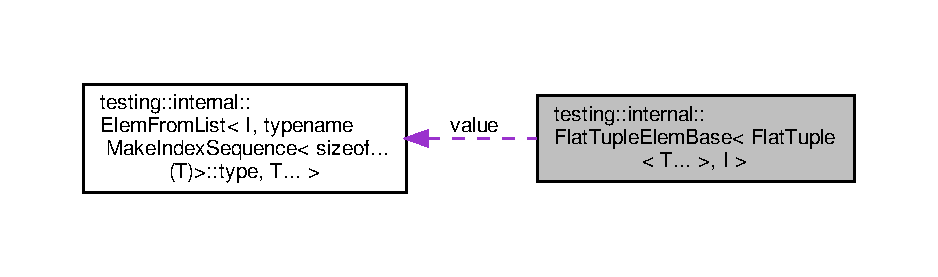
\includegraphics[width=350pt]{structtesting_1_1internal_1_1FlatTupleElemBase_3_01FlatTuple_3_01T_8_8_8_01_4_00_01I_01_4__coll__graph}
\end{center}
\end{figure}
\subsection*{Public Types}
\begin{DoxyCompactItemize}
\item 
using \hyperlink{structtesting_1_1internal_1_1FlatTupleElemBase_3_01FlatTuple_3_01T_8_8_8_01_4_00_01I_01_4_a6b87a445f87724f9363b348e6c697766}{value\+\_\+type} = typename \hyperlink{structtesting_1_1internal_1_1ElemFromList}{Elem\+From\+List}$<$ I, typename \hyperlink{structtesting_1_1internal_1_1MakeIndexSequence}{Make\+Index\+Sequence}$<$ sizeof...(T)$>$\+::type, T... $>$\+::type
\end{DoxyCompactItemize}
\subsection*{Public Member Functions}
\begin{DoxyCompactItemize}
\item 
\hyperlink{structtesting_1_1internal_1_1FlatTupleElemBase_3_01FlatTuple_3_01T_8_8_8_01_4_00_01I_01_4_a7b460283c4ba5ad116a4305d05155546}{Flat\+Tuple\+Elem\+Base} ()=default
\item 
\hyperlink{structtesting_1_1internal_1_1FlatTupleElemBase_3_01FlatTuple_3_01T_8_8_8_01_4_00_01I_01_4_a153da382b00977dfb5974f85dd31ea58}{Flat\+Tuple\+Elem\+Base} (\hyperlink{structtesting_1_1internal_1_1FlatTupleElemBase_3_01FlatTuple_3_01T_8_8_8_01_4_00_01I_01_4_a6b87a445f87724f9363b348e6c697766}{value\+\_\+type} t)
\end{DoxyCompactItemize}
\subsection*{Public Attributes}
\begin{DoxyCompactItemize}
\item 
\hyperlink{structtesting_1_1internal_1_1FlatTupleElemBase_3_01FlatTuple_3_01T_8_8_8_01_4_00_01I_01_4_a6b87a445f87724f9363b348e6c697766}{value\+\_\+type} \hyperlink{structtesting_1_1internal_1_1FlatTupleElemBase_3_01FlatTuple_3_01T_8_8_8_01_4_00_01I_01_4_ac175518e7807c0b49c0ba8c1c78269ec}{value}
\end{DoxyCompactItemize}


\subsection{Member Typedef Documentation}
\mbox{\Hypertarget{structtesting_1_1internal_1_1FlatTupleElemBase_3_01FlatTuple_3_01T_8_8_8_01_4_00_01I_01_4_a6b87a445f87724f9363b348e6c697766}\label{structtesting_1_1internal_1_1FlatTupleElemBase_3_01FlatTuple_3_01T_8_8_8_01_4_00_01I_01_4_a6b87a445f87724f9363b348e6c697766}} 
\index{testing\+::internal\+::\+Flat\+Tuple\+Elem\+Base$<$ Flat\+Tuple$<$ T... $>$, I $>$@{testing\+::internal\+::\+Flat\+Tuple\+Elem\+Base$<$ Flat\+Tuple$<$ T... $>$, I $>$}!value\+\_\+type@{value\+\_\+type}}
\index{value\+\_\+type@{value\+\_\+type}!testing\+::internal\+::\+Flat\+Tuple\+Elem\+Base$<$ Flat\+Tuple$<$ T... $>$, I $>$@{testing\+::internal\+::\+Flat\+Tuple\+Elem\+Base$<$ Flat\+Tuple$<$ T... $>$, I $>$}}
\subsubsection{\texorpdfstring{value\+\_\+type}{value\_type}}
{\footnotesize\ttfamily template$<$typename... T, size\+\_\+t I$>$ \\
using \hyperlink{structtesting_1_1internal_1_1FlatTupleElemBase}{testing\+::internal\+::\+Flat\+Tuple\+Elem\+Base}$<$ \hyperlink{classtesting_1_1internal_1_1FlatTuple}{Flat\+Tuple}$<$ T... $>$, I $>$\+::\hyperlink{structtesting_1_1internal_1_1FlatTupleElemBase_3_01FlatTuple_3_01T_8_8_8_01_4_00_01I_01_4_a6b87a445f87724f9363b348e6c697766}{value\+\_\+type} =  typename \hyperlink{structtesting_1_1internal_1_1ElemFromList}{Elem\+From\+List}$<$I, typename \hyperlink{structtesting_1_1internal_1_1MakeIndexSequence}{Make\+Index\+Sequence}$<$sizeof...(T)$>$\+::type, T...$>$\+::type}



\subsection{Constructor \& Destructor Documentation}
\mbox{\Hypertarget{structtesting_1_1internal_1_1FlatTupleElemBase_3_01FlatTuple_3_01T_8_8_8_01_4_00_01I_01_4_a7b460283c4ba5ad116a4305d05155546}\label{structtesting_1_1internal_1_1FlatTupleElemBase_3_01FlatTuple_3_01T_8_8_8_01_4_00_01I_01_4_a7b460283c4ba5ad116a4305d05155546}} 
\index{testing\+::internal\+::\+Flat\+Tuple\+Elem\+Base$<$ Flat\+Tuple$<$ T... $>$, I $>$@{testing\+::internal\+::\+Flat\+Tuple\+Elem\+Base$<$ Flat\+Tuple$<$ T... $>$, I $>$}!Flat\+Tuple\+Elem\+Base@{Flat\+Tuple\+Elem\+Base}}
\index{Flat\+Tuple\+Elem\+Base@{Flat\+Tuple\+Elem\+Base}!testing\+::internal\+::\+Flat\+Tuple\+Elem\+Base$<$ Flat\+Tuple$<$ T... $>$, I $>$@{testing\+::internal\+::\+Flat\+Tuple\+Elem\+Base$<$ Flat\+Tuple$<$ T... $>$, I $>$}}
\subsubsection{\texorpdfstring{Flat\+Tuple\+Elem\+Base()}{FlatTupleElemBase()}\hspace{0.1cm}{\footnotesize\ttfamily [1/2]}}
{\footnotesize\ttfamily template$<$typename... T, size\+\_\+t I$>$ \\
\hyperlink{structtesting_1_1internal_1_1FlatTupleElemBase}{testing\+::internal\+::\+Flat\+Tuple\+Elem\+Base}$<$ \hyperlink{classtesting_1_1internal_1_1FlatTuple}{Flat\+Tuple}$<$ T... $>$, I $>$\+::\hyperlink{structtesting_1_1internal_1_1FlatTupleElemBase}{Flat\+Tuple\+Elem\+Base} (\begin{DoxyParamCaption}{ }\end{DoxyParamCaption})\hspace{0.3cm}{\ttfamily [default]}}

\mbox{\Hypertarget{structtesting_1_1internal_1_1FlatTupleElemBase_3_01FlatTuple_3_01T_8_8_8_01_4_00_01I_01_4_a153da382b00977dfb5974f85dd31ea58}\label{structtesting_1_1internal_1_1FlatTupleElemBase_3_01FlatTuple_3_01T_8_8_8_01_4_00_01I_01_4_a153da382b00977dfb5974f85dd31ea58}} 
\index{testing\+::internal\+::\+Flat\+Tuple\+Elem\+Base$<$ Flat\+Tuple$<$ T... $>$, I $>$@{testing\+::internal\+::\+Flat\+Tuple\+Elem\+Base$<$ Flat\+Tuple$<$ T... $>$, I $>$}!Flat\+Tuple\+Elem\+Base@{Flat\+Tuple\+Elem\+Base}}
\index{Flat\+Tuple\+Elem\+Base@{Flat\+Tuple\+Elem\+Base}!testing\+::internal\+::\+Flat\+Tuple\+Elem\+Base$<$ Flat\+Tuple$<$ T... $>$, I $>$@{testing\+::internal\+::\+Flat\+Tuple\+Elem\+Base$<$ Flat\+Tuple$<$ T... $>$, I $>$}}
\subsubsection{\texorpdfstring{Flat\+Tuple\+Elem\+Base()}{FlatTupleElemBase()}\hspace{0.1cm}{\footnotesize\ttfamily [2/2]}}
{\footnotesize\ttfamily template$<$typename... T, size\+\_\+t I$>$ \\
\hyperlink{structtesting_1_1internal_1_1FlatTupleElemBase}{testing\+::internal\+::\+Flat\+Tuple\+Elem\+Base}$<$ \hyperlink{classtesting_1_1internal_1_1FlatTuple}{Flat\+Tuple}$<$ T... $>$, I $>$\+::\hyperlink{structtesting_1_1internal_1_1FlatTupleElemBase}{Flat\+Tuple\+Elem\+Base} (\begin{DoxyParamCaption}\item[{\hyperlink{structtesting_1_1internal_1_1FlatTupleElemBase_3_01FlatTuple_3_01T_8_8_8_01_4_00_01I_01_4_a6b87a445f87724f9363b348e6c697766}{value\+\_\+type}}]{t }\end{DoxyParamCaption})\hspace{0.3cm}{\ttfamily [inline]}, {\ttfamily [explicit]}}



\subsection{Member Data Documentation}
\mbox{\Hypertarget{structtesting_1_1internal_1_1FlatTupleElemBase_3_01FlatTuple_3_01T_8_8_8_01_4_00_01I_01_4_ac175518e7807c0b49c0ba8c1c78269ec}\label{structtesting_1_1internal_1_1FlatTupleElemBase_3_01FlatTuple_3_01T_8_8_8_01_4_00_01I_01_4_ac175518e7807c0b49c0ba8c1c78269ec}} 
\index{testing\+::internal\+::\+Flat\+Tuple\+Elem\+Base$<$ Flat\+Tuple$<$ T... $>$, I $>$@{testing\+::internal\+::\+Flat\+Tuple\+Elem\+Base$<$ Flat\+Tuple$<$ T... $>$, I $>$}!value@{value}}
\index{value@{value}!testing\+::internal\+::\+Flat\+Tuple\+Elem\+Base$<$ Flat\+Tuple$<$ T... $>$, I $>$@{testing\+::internal\+::\+Flat\+Tuple\+Elem\+Base$<$ Flat\+Tuple$<$ T... $>$, I $>$}}
\subsubsection{\texorpdfstring{value}{value}}
{\footnotesize\ttfamily template$<$typename... T, size\+\_\+t I$>$ \\
\hyperlink{structtesting_1_1internal_1_1FlatTupleElemBase_3_01FlatTuple_3_01T_8_8_8_01_4_00_01I_01_4_a6b87a445f87724f9363b348e6c697766}{value\+\_\+type} \hyperlink{structtesting_1_1internal_1_1FlatTupleElemBase}{testing\+::internal\+::\+Flat\+Tuple\+Elem\+Base}$<$ \hyperlink{classtesting_1_1internal_1_1FlatTuple}{Flat\+Tuple}$<$ T... $>$, I $>$\+::value}



The documentation for this struct was generated from the following file\+:\begin{DoxyCompactItemize}
\item 
tests/googletest/include/gtest/internal/\hyperlink{gtest-internal_8h}{gtest-\/internal.\+h}\end{DoxyCompactItemize}

\hypertarget{classtesting_1_1internal_1_1FloatingPoint}{}\section{testing\+:\+:internal\+:\+:Floating\+Point$<$ Raw\+Type $>$ Class Template Reference}
\label{classtesting_1_1internal_1_1FloatingPoint}\index{testing\+::internal\+::\+Floating\+Point$<$ Raw\+Type $>$@{testing\+::internal\+::\+Floating\+Point$<$ Raw\+Type $>$}}


{\ttfamily \#include $<$gtest-\/internal.\+h$>$}



Collaboration diagram for testing\+:\+:internal\+:\+:Floating\+Point$<$ Raw\+Type $>$\+:\nopagebreak
\begin{figure}[H]
\begin{center}
\leavevmode
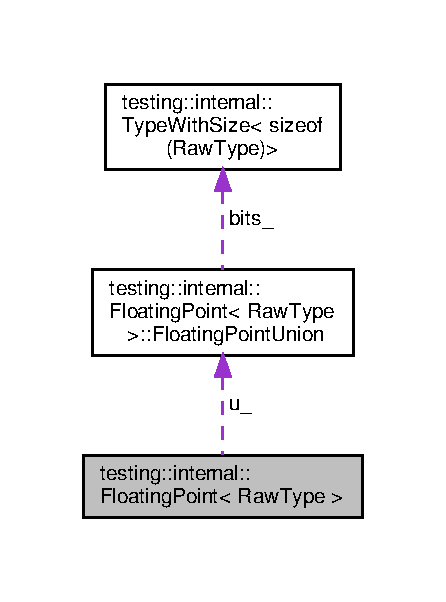
\includegraphics[width=214pt]{classtesting_1_1internal_1_1FloatingPoint__coll__graph}
\end{center}
\end{figure}
\subsection*{Classes}
\begin{DoxyCompactItemize}
\item 
union \hyperlink{uniontesting_1_1internal_1_1FloatingPoint_1_1FloatingPointUnion}{Floating\+Point\+Union}
\end{DoxyCompactItemize}
\subsection*{Public Types}
\begin{DoxyCompactItemize}
\item 
typedef \hyperlink{classtesting_1_1internal_1_1TypeWithSize}{Type\+With\+Size}$<$ sizeof(Raw\+Type)$>$\+::U\+Int \hyperlink{classtesting_1_1internal_1_1FloatingPoint_abf228bf6cd48f12c8b44c85b4971a731}{Bits}
\end{DoxyCompactItemize}
\subsection*{Public Member Functions}
\begin{DoxyCompactItemize}
\item 
\hyperlink{classtesting_1_1internal_1_1FloatingPoint_a0dabf840863e0df84046f171c891fe71}{Floating\+Point} (const Raw\+Type \&x)
\item 
const \hyperlink{classtesting_1_1internal_1_1FloatingPoint_abf228bf6cd48f12c8b44c85b4971a731}{Bits} \& \hyperlink{classtesting_1_1internal_1_1FloatingPoint_aab053be914bdc9e507c0db89740c318c}{bits} () const
\item 
\hyperlink{classtesting_1_1internal_1_1FloatingPoint_abf228bf6cd48f12c8b44c85b4971a731}{Bits} \hyperlink{classtesting_1_1internal_1_1FloatingPoint_af6bf8fab8df572ecb137a3516ff390ae}{exponent\+\_\+bits} () const
\item 
\hyperlink{classtesting_1_1internal_1_1FloatingPoint_abf228bf6cd48f12c8b44c85b4971a731}{Bits} \hyperlink{classtesting_1_1internal_1_1FloatingPoint_aa17337e50a2ac855719bc0676529558f}{fraction\+\_\+bits} () const
\item 
\hyperlink{classtesting_1_1internal_1_1FloatingPoint_abf228bf6cd48f12c8b44c85b4971a731}{Bits} \hyperlink{classtesting_1_1internal_1_1FloatingPoint_afb8a816bb598225d775caaf43a893ef0}{sign\+\_\+bit} () const
\item 
bool \hyperlink{classtesting_1_1internal_1_1FloatingPoint_a1fc654fd206efa98e480aa1e034f30d5}{is\+\_\+nan} () const
\item 
bool \hyperlink{classtesting_1_1internal_1_1FloatingPoint_a965214c1af2f9ac5adb1393794aa81e5}{Almost\+Equals} (const \hyperlink{classtesting_1_1internal_1_1FloatingPoint}{Floating\+Point} \&rhs) const
\item 
{\footnotesize template$<$$>$ }\\float \hyperlink{classtesting_1_1internal_1_1FloatingPoint_af2eda9331e679229a1baa3404b57b51d}{Max} ()
\item 
{\footnotesize template$<$$>$ }\\double \hyperlink{classtesting_1_1internal_1_1FloatingPoint_afc2e85c0e886cb13b2300e961c9a9648}{Max} ()
\end{DoxyCompactItemize}
\subsection*{Static Public Member Functions}
\begin{DoxyCompactItemize}
\item 
static Raw\+Type \hyperlink{classtesting_1_1internal_1_1FloatingPoint_ac551f793522e54fbd8a25acb79eac5b1}{Reinterpret\+Bits} (const \hyperlink{classtesting_1_1internal_1_1FloatingPoint_abf228bf6cd48f12c8b44c85b4971a731}{Bits} \hyperlink{classtesting_1_1internal_1_1FloatingPoint_aab053be914bdc9e507c0db89740c318c}{bits})
\item 
static Raw\+Type \hyperlink{classtesting_1_1internal_1_1FloatingPoint_a460027cc19cf01ae8e09cc3796b2b575}{Infinity} ()
\item 
static Raw\+Type \hyperlink{classtesting_1_1internal_1_1FloatingPoint_aae5954d8a57d3ff0987c6930cb68e114}{Max} ()
\end{DoxyCompactItemize}
\subsection*{Static Public Attributes}
\begin{DoxyCompactItemize}
\item 
static const size\+\_\+t \hyperlink{classtesting_1_1internal_1_1FloatingPoint_ab819d2e8f93e9e482373999f0f8d71b9}{k\+Bit\+Count} = 8$\ast$sizeof(Raw\+Type)
\item 
static const size\+\_\+t \hyperlink{classtesting_1_1internal_1_1FloatingPoint_a0b756a6d2a4f5f5b41ca79651c06c043}{k\+Fraction\+Bit\+Count}
\item 
static const size\+\_\+t \hyperlink{classtesting_1_1internal_1_1FloatingPoint_a1973d843c00781053d3073daa8a40119}{k\+Exponent\+Bit\+Count} = \hyperlink{classtesting_1_1internal_1_1FloatingPoint_ab819d2e8f93e9e482373999f0f8d71b9}{k\+Bit\+Count} -\/ 1 -\/ \hyperlink{classtesting_1_1internal_1_1FloatingPoint_a0b756a6d2a4f5f5b41ca79651c06c043}{k\+Fraction\+Bit\+Count}
\item 
static const \hyperlink{classtesting_1_1internal_1_1FloatingPoint_abf228bf6cd48f12c8b44c85b4971a731}{Bits} \hyperlink{classtesting_1_1internal_1_1FloatingPoint_aca98b5ea6f2222a66a82e52421682efa}{k\+Sign\+Bit\+Mask} = static\+\_\+cast$<$\hyperlink{classtesting_1_1internal_1_1FloatingPoint_abf228bf6cd48f12c8b44c85b4971a731}{Bits}$>$(1) $<$$<$ (\hyperlink{classtesting_1_1internal_1_1FloatingPoint_ab819d2e8f93e9e482373999f0f8d71b9}{k\+Bit\+Count} -\/ 1)
\item 
static const \hyperlink{classtesting_1_1internal_1_1FloatingPoint_abf228bf6cd48f12c8b44c85b4971a731}{Bits} \hyperlink{classtesting_1_1internal_1_1FloatingPoint_a0ac75d4ffd24f14bca452abe8a718da1}{k\+Fraction\+Bit\+Mask}
\item 
static const \hyperlink{classtesting_1_1internal_1_1FloatingPoint_abf228bf6cd48f12c8b44c85b4971a731}{Bits} \hyperlink{classtesting_1_1internal_1_1FloatingPoint_a66065dfc4d5f41100f686159637af23b}{k\+Exponent\+Bit\+Mask} = $\sim$(\hyperlink{classtesting_1_1internal_1_1FloatingPoint_aca98b5ea6f2222a66a82e52421682efa}{k\+Sign\+Bit\+Mask} $\vert$ \hyperlink{classtesting_1_1internal_1_1FloatingPoint_a0ac75d4ffd24f14bca452abe8a718da1}{k\+Fraction\+Bit\+Mask})
\item 
static const size\+\_\+t \hyperlink{classtesting_1_1internal_1_1FloatingPoint_aac498b3714d93f8e88cdc30e4c5935f6}{k\+Max\+Ulps} = 4
\end{DoxyCompactItemize}
\subsection*{Static Private Member Functions}
\begin{DoxyCompactItemize}
\item 
static \hyperlink{classtesting_1_1internal_1_1FloatingPoint_abf228bf6cd48f12c8b44c85b4971a731}{Bits} \hyperlink{classtesting_1_1internal_1_1FloatingPoint_a2cf0e39c6ebf026bc0353100d031ca85}{Sign\+And\+Magnitude\+To\+Biased} (const \hyperlink{classtesting_1_1internal_1_1FloatingPoint_abf228bf6cd48f12c8b44c85b4971a731}{Bits} \&sam)
\item 
static \hyperlink{classtesting_1_1internal_1_1FloatingPoint_abf228bf6cd48f12c8b44c85b4971a731}{Bits} \hyperlink{classtesting_1_1internal_1_1FloatingPoint_afe00f9f26ad2929a061f7e07b8a5071a}{Distance\+Between\+Sign\+And\+Magnitude\+Numbers} (const \hyperlink{classtesting_1_1internal_1_1FloatingPoint_abf228bf6cd48f12c8b44c85b4971a731}{Bits} \&sam1, const \hyperlink{classtesting_1_1internal_1_1FloatingPoint_abf228bf6cd48f12c8b44c85b4971a731}{Bits} \&sam2)
\end{DoxyCompactItemize}
\subsection*{Private Attributes}
\begin{DoxyCompactItemize}
\item 
\hyperlink{uniontesting_1_1internal_1_1FloatingPoint_1_1FloatingPointUnion}{Floating\+Point\+Union} \hyperlink{classtesting_1_1internal_1_1FloatingPoint_a2e0b6bd427248b91476f3fca281f7104}{u\+\_\+}
\end{DoxyCompactItemize}


\subsection{Member Typedef Documentation}
\mbox{\Hypertarget{classtesting_1_1internal_1_1FloatingPoint_abf228bf6cd48f12c8b44c85b4971a731}\label{classtesting_1_1internal_1_1FloatingPoint_abf228bf6cd48f12c8b44c85b4971a731}} 
\index{testing\+::internal\+::\+Floating\+Point@{testing\+::internal\+::\+Floating\+Point}!Bits@{Bits}}
\index{Bits@{Bits}!testing\+::internal\+::\+Floating\+Point@{testing\+::internal\+::\+Floating\+Point}}
\subsubsection{\texorpdfstring{Bits}{Bits}}
{\footnotesize\ttfamily template$<$typename Raw\+Type$>$ \\
typedef \hyperlink{classtesting_1_1internal_1_1TypeWithSize}{Type\+With\+Size}$<$sizeof(Raw\+Type)$>$\+::U\+Int \hyperlink{classtesting_1_1internal_1_1FloatingPoint}{testing\+::internal\+::\+Floating\+Point}$<$ Raw\+Type $>$\+::\hyperlink{classtesting_1_1internal_1_1FloatingPoint_abf228bf6cd48f12c8b44c85b4971a731}{Bits}}



\subsection{Constructor \& Destructor Documentation}
\mbox{\Hypertarget{classtesting_1_1internal_1_1FloatingPoint_a0dabf840863e0df84046f171c891fe71}\label{classtesting_1_1internal_1_1FloatingPoint_a0dabf840863e0df84046f171c891fe71}} 
\index{testing\+::internal\+::\+Floating\+Point@{testing\+::internal\+::\+Floating\+Point}!Floating\+Point@{Floating\+Point}}
\index{Floating\+Point@{Floating\+Point}!testing\+::internal\+::\+Floating\+Point@{testing\+::internal\+::\+Floating\+Point}}
\subsubsection{\texorpdfstring{Floating\+Point()}{FloatingPoint()}}
{\footnotesize\ttfamily template$<$typename Raw\+Type$>$ \\
\hyperlink{classtesting_1_1internal_1_1FloatingPoint}{testing\+::internal\+::\+Floating\+Point}$<$ Raw\+Type $>$\+::\hyperlink{classtesting_1_1internal_1_1FloatingPoint}{Floating\+Point} (\begin{DoxyParamCaption}\item[{const Raw\+Type \&}]{x }\end{DoxyParamCaption})\hspace{0.3cm}{\ttfamily [inline]}, {\ttfamily [explicit]}}



\subsection{Member Function Documentation}
\mbox{\Hypertarget{classtesting_1_1internal_1_1FloatingPoint_a965214c1af2f9ac5adb1393794aa81e5}\label{classtesting_1_1internal_1_1FloatingPoint_a965214c1af2f9ac5adb1393794aa81e5}} 
\index{testing\+::internal\+::\+Floating\+Point@{testing\+::internal\+::\+Floating\+Point}!Almost\+Equals@{Almost\+Equals}}
\index{Almost\+Equals@{Almost\+Equals}!testing\+::internal\+::\+Floating\+Point@{testing\+::internal\+::\+Floating\+Point}}
\subsubsection{\texorpdfstring{Almost\+Equals()}{AlmostEquals()}}
{\footnotesize\ttfamily template$<$typename Raw\+Type$>$ \\
bool \hyperlink{classtesting_1_1internal_1_1FloatingPoint}{testing\+::internal\+::\+Floating\+Point}$<$ Raw\+Type $>$\+::Almost\+Equals (\begin{DoxyParamCaption}\item[{const \hyperlink{classtesting_1_1internal_1_1FloatingPoint}{Floating\+Point}$<$ Raw\+Type $>$ \&}]{rhs }\end{DoxyParamCaption}) const\hspace{0.3cm}{\ttfamily [inline]}}

\mbox{\Hypertarget{classtesting_1_1internal_1_1FloatingPoint_aab053be914bdc9e507c0db89740c318c}\label{classtesting_1_1internal_1_1FloatingPoint_aab053be914bdc9e507c0db89740c318c}} 
\index{testing\+::internal\+::\+Floating\+Point@{testing\+::internal\+::\+Floating\+Point}!bits@{bits}}
\index{bits@{bits}!testing\+::internal\+::\+Floating\+Point@{testing\+::internal\+::\+Floating\+Point}}
\subsubsection{\texorpdfstring{bits()}{bits()}}
{\footnotesize\ttfamily template$<$typename Raw\+Type$>$ \\
const \hyperlink{classtesting_1_1internal_1_1FloatingPoint_abf228bf6cd48f12c8b44c85b4971a731}{Bits}\& \hyperlink{classtesting_1_1internal_1_1FloatingPoint}{testing\+::internal\+::\+Floating\+Point}$<$ Raw\+Type $>$\+::bits (\begin{DoxyParamCaption}{ }\end{DoxyParamCaption}) const\hspace{0.3cm}{\ttfamily [inline]}}

\mbox{\Hypertarget{classtesting_1_1internal_1_1FloatingPoint_afe00f9f26ad2929a061f7e07b8a5071a}\label{classtesting_1_1internal_1_1FloatingPoint_afe00f9f26ad2929a061f7e07b8a5071a}} 
\index{testing\+::internal\+::\+Floating\+Point@{testing\+::internal\+::\+Floating\+Point}!Distance\+Between\+Sign\+And\+Magnitude\+Numbers@{Distance\+Between\+Sign\+And\+Magnitude\+Numbers}}
\index{Distance\+Between\+Sign\+And\+Magnitude\+Numbers@{Distance\+Between\+Sign\+And\+Magnitude\+Numbers}!testing\+::internal\+::\+Floating\+Point@{testing\+::internal\+::\+Floating\+Point}}
\subsubsection{\texorpdfstring{Distance\+Between\+Sign\+And\+Magnitude\+Numbers()}{DistanceBetweenSignAndMagnitudeNumbers()}}
{\footnotesize\ttfamily template$<$typename Raw\+Type$>$ \\
static \hyperlink{classtesting_1_1internal_1_1FloatingPoint_abf228bf6cd48f12c8b44c85b4971a731}{Bits} \hyperlink{classtesting_1_1internal_1_1FloatingPoint}{testing\+::internal\+::\+Floating\+Point}$<$ Raw\+Type $>$\+::Distance\+Between\+Sign\+And\+Magnitude\+Numbers (\begin{DoxyParamCaption}\item[{const \hyperlink{classtesting_1_1internal_1_1FloatingPoint_abf228bf6cd48f12c8b44c85b4971a731}{Bits} \&}]{sam1,  }\item[{const \hyperlink{classtesting_1_1internal_1_1FloatingPoint_abf228bf6cd48f12c8b44c85b4971a731}{Bits} \&}]{sam2 }\end{DoxyParamCaption})\hspace{0.3cm}{\ttfamily [inline]}, {\ttfamily [static]}, {\ttfamily [private]}}

\mbox{\Hypertarget{classtesting_1_1internal_1_1FloatingPoint_af6bf8fab8df572ecb137a3516ff390ae}\label{classtesting_1_1internal_1_1FloatingPoint_af6bf8fab8df572ecb137a3516ff390ae}} 
\index{testing\+::internal\+::\+Floating\+Point@{testing\+::internal\+::\+Floating\+Point}!exponent\+\_\+bits@{exponent\+\_\+bits}}
\index{exponent\+\_\+bits@{exponent\+\_\+bits}!testing\+::internal\+::\+Floating\+Point@{testing\+::internal\+::\+Floating\+Point}}
\subsubsection{\texorpdfstring{exponent\+\_\+bits()}{exponent\_bits()}}
{\footnotesize\ttfamily template$<$typename Raw\+Type$>$ \\
\hyperlink{classtesting_1_1internal_1_1FloatingPoint_abf228bf6cd48f12c8b44c85b4971a731}{Bits} \hyperlink{classtesting_1_1internal_1_1FloatingPoint}{testing\+::internal\+::\+Floating\+Point}$<$ Raw\+Type $>$\+::exponent\+\_\+bits (\begin{DoxyParamCaption}{ }\end{DoxyParamCaption}) const\hspace{0.3cm}{\ttfamily [inline]}}

\mbox{\Hypertarget{classtesting_1_1internal_1_1FloatingPoint_aa17337e50a2ac855719bc0676529558f}\label{classtesting_1_1internal_1_1FloatingPoint_aa17337e50a2ac855719bc0676529558f}} 
\index{testing\+::internal\+::\+Floating\+Point@{testing\+::internal\+::\+Floating\+Point}!fraction\+\_\+bits@{fraction\+\_\+bits}}
\index{fraction\+\_\+bits@{fraction\+\_\+bits}!testing\+::internal\+::\+Floating\+Point@{testing\+::internal\+::\+Floating\+Point}}
\subsubsection{\texorpdfstring{fraction\+\_\+bits()}{fraction\_bits()}}
{\footnotesize\ttfamily template$<$typename Raw\+Type$>$ \\
\hyperlink{classtesting_1_1internal_1_1FloatingPoint_abf228bf6cd48f12c8b44c85b4971a731}{Bits} \hyperlink{classtesting_1_1internal_1_1FloatingPoint}{testing\+::internal\+::\+Floating\+Point}$<$ Raw\+Type $>$\+::fraction\+\_\+bits (\begin{DoxyParamCaption}{ }\end{DoxyParamCaption}) const\hspace{0.3cm}{\ttfamily [inline]}}

\mbox{\Hypertarget{classtesting_1_1internal_1_1FloatingPoint_a460027cc19cf01ae8e09cc3796b2b575}\label{classtesting_1_1internal_1_1FloatingPoint_a460027cc19cf01ae8e09cc3796b2b575}} 
\index{testing\+::internal\+::\+Floating\+Point@{testing\+::internal\+::\+Floating\+Point}!Infinity@{Infinity}}
\index{Infinity@{Infinity}!testing\+::internal\+::\+Floating\+Point@{testing\+::internal\+::\+Floating\+Point}}
\subsubsection{\texorpdfstring{Infinity()}{Infinity()}}
{\footnotesize\ttfamily template$<$typename Raw\+Type$>$ \\
static Raw\+Type \hyperlink{classtesting_1_1internal_1_1FloatingPoint}{testing\+::internal\+::\+Floating\+Point}$<$ Raw\+Type $>$\+::Infinity (\begin{DoxyParamCaption}{ }\end{DoxyParamCaption})\hspace{0.3cm}{\ttfamily [inline]}, {\ttfamily [static]}}

\mbox{\Hypertarget{classtesting_1_1internal_1_1FloatingPoint_a1fc654fd206efa98e480aa1e034f30d5}\label{classtesting_1_1internal_1_1FloatingPoint_a1fc654fd206efa98e480aa1e034f30d5}} 
\index{testing\+::internal\+::\+Floating\+Point@{testing\+::internal\+::\+Floating\+Point}!is\+\_\+nan@{is\+\_\+nan}}
\index{is\+\_\+nan@{is\+\_\+nan}!testing\+::internal\+::\+Floating\+Point@{testing\+::internal\+::\+Floating\+Point}}
\subsubsection{\texorpdfstring{is\+\_\+nan()}{is\_nan()}}
{\footnotesize\ttfamily template$<$typename Raw\+Type$>$ \\
bool \hyperlink{classtesting_1_1internal_1_1FloatingPoint}{testing\+::internal\+::\+Floating\+Point}$<$ Raw\+Type $>$\+::is\+\_\+nan (\begin{DoxyParamCaption}{ }\end{DoxyParamCaption}) const\hspace{0.3cm}{\ttfamily [inline]}}

\mbox{\Hypertarget{classtesting_1_1internal_1_1FloatingPoint_aae5954d8a57d3ff0987c6930cb68e114}\label{classtesting_1_1internal_1_1FloatingPoint_aae5954d8a57d3ff0987c6930cb68e114}} 
\index{testing\+::internal\+::\+Floating\+Point@{testing\+::internal\+::\+Floating\+Point}!Max@{Max}}
\index{Max@{Max}!testing\+::internal\+::\+Floating\+Point@{testing\+::internal\+::\+Floating\+Point}}
\subsubsection{\texorpdfstring{Max()}{Max()}\hspace{0.1cm}{\footnotesize\ttfamily [1/3]}}
{\footnotesize\ttfamily template$<$typename Raw\+Type$>$ \\
static Raw\+Type \hyperlink{classtesting_1_1internal_1_1FloatingPoint}{testing\+::internal\+::\+Floating\+Point}$<$ Raw\+Type $>$\+::Max (\begin{DoxyParamCaption}{ }\end{DoxyParamCaption})\hspace{0.3cm}{\ttfamily [static]}}

\mbox{\Hypertarget{classtesting_1_1internal_1_1FloatingPoint_af2eda9331e679229a1baa3404b57b51d}\label{classtesting_1_1internal_1_1FloatingPoint_af2eda9331e679229a1baa3404b57b51d}} 
\index{testing\+::internal\+::\+Floating\+Point@{testing\+::internal\+::\+Floating\+Point}!Max@{Max}}
\index{Max@{Max}!testing\+::internal\+::\+Floating\+Point@{testing\+::internal\+::\+Floating\+Point}}
\subsubsection{\texorpdfstring{Max()}{Max()}\hspace{0.1cm}{\footnotesize\ttfamily [2/3]}}
{\footnotesize\ttfamily template$<$$>$ \\
float \hyperlink{classtesting_1_1internal_1_1FloatingPoint}{testing\+::internal\+::\+Floating\+Point}$<$ float $>$\+::Max (\begin{DoxyParamCaption}{ }\end{DoxyParamCaption})\hspace{0.3cm}{\ttfamily [inline]}}

\mbox{\Hypertarget{classtesting_1_1internal_1_1FloatingPoint_afc2e85c0e886cb13b2300e961c9a9648}\label{classtesting_1_1internal_1_1FloatingPoint_afc2e85c0e886cb13b2300e961c9a9648}} 
\index{testing\+::internal\+::\+Floating\+Point@{testing\+::internal\+::\+Floating\+Point}!Max@{Max}}
\index{Max@{Max}!testing\+::internal\+::\+Floating\+Point@{testing\+::internal\+::\+Floating\+Point}}
\subsubsection{\texorpdfstring{Max()}{Max()}\hspace{0.1cm}{\footnotesize\ttfamily [3/3]}}
{\footnotesize\ttfamily template$<$$>$ \\
double \hyperlink{classtesting_1_1internal_1_1FloatingPoint}{testing\+::internal\+::\+Floating\+Point}$<$ double $>$\+::Max (\begin{DoxyParamCaption}{ }\end{DoxyParamCaption})\hspace{0.3cm}{\ttfamily [inline]}}

\mbox{\Hypertarget{classtesting_1_1internal_1_1FloatingPoint_ac551f793522e54fbd8a25acb79eac5b1}\label{classtesting_1_1internal_1_1FloatingPoint_ac551f793522e54fbd8a25acb79eac5b1}} 
\index{testing\+::internal\+::\+Floating\+Point@{testing\+::internal\+::\+Floating\+Point}!Reinterpret\+Bits@{Reinterpret\+Bits}}
\index{Reinterpret\+Bits@{Reinterpret\+Bits}!testing\+::internal\+::\+Floating\+Point@{testing\+::internal\+::\+Floating\+Point}}
\subsubsection{\texorpdfstring{Reinterpret\+Bits()}{ReinterpretBits()}}
{\footnotesize\ttfamily template$<$typename Raw\+Type$>$ \\
static Raw\+Type \hyperlink{classtesting_1_1internal_1_1FloatingPoint}{testing\+::internal\+::\+Floating\+Point}$<$ Raw\+Type $>$\+::Reinterpret\+Bits (\begin{DoxyParamCaption}\item[{const \hyperlink{classtesting_1_1internal_1_1FloatingPoint_abf228bf6cd48f12c8b44c85b4971a731}{Bits}}]{bits }\end{DoxyParamCaption})\hspace{0.3cm}{\ttfamily [inline]}, {\ttfamily [static]}}

\mbox{\Hypertarget{classtesting_1_1internal_1_1FloatingPoint_afb8a816bb598225d775caaf43a893ef0}\label{classtesting_1_1internal_1_1FloatingPoint_afb8a816bb598225d775caaf43a893ef0}} 
\index{testing\+::internal\+::\+Floating\+Point@{testing\+::internal\+::\+Floating\+Point}!sign\+\_\+bit@{sign\+\_\+bit}}
\index{sign\+\_\+bit@{sign\+\_\+bit}!testing\+::internal\+::\+Floating\+Point@{testing\+::internal\+::\+Floating\+Point}}
\subsubsection{\texorpdfstring{sign\+\_\+bit()}{sign\_bit()}}
{\footnotesize\ttfamily template$<$typename Raw\+Type$>$ \\
\hyperlink{classtesting_1_1internal_1_1FloatingPoint_abf228bf6cd48f12c8b44c85b4971a731}{Bits} \hyperlink{classtesting_1_1internal_1_1FloatingPoint}{testing\+::internal\+::\+Floating\+Point}$<$ Raw\+Type $>$\+::sign\+\_\+bit (\begin{DoxyParamCaption}{ }\end{DoxyParamCaption}) const\hspace{0.3cm}{\ttfamily [inline]}}

\mbox{\Hypertarget{classtesting_1_1internal_1_1FloatingPoint_a2cf0e39c6ebf026bc0353100d031ca85}\label{classtesting_1_1internal_1_1FloatingPoint_a2cf0e39c6ebf026bc0353100d031ca85}} 
\index{testing\+::internal\+::\+Floating\+Point@{testing\+::internal\+::\+Floating\+Point}!Sign\+And\+Magnitude\+To\+Biased@{Sign\+And\+Magnitude\+To\+Biased}}
\index{Sign\+And\+Magnitude\+To\+Biased@{Sign\+And\+Magnitude\+To\+Biased}!testing\+::internal\+::\+Floating\+Point@{testing\+::internal\+::\+Floating\+Point}}
\subsubsection{\texorpdfstring{Sign\+And\+Magnitude\+To\+Biased()}{SignAndMagnitudeToBiased()}}
{\footnotesize\ttfamily template$<$typename Raw\+Type$>$ \\
static \hyperlink{classtesting_1_1internal_1_1FloatingPoint_abf228bf6cd48f12c8b44c85b4971a731}{Bits} \hyperlink{classtesting_1_1internal_1_1FloatingPoint}{testing\+::internal\+::\+Floating\+Point}$<$ Raw\+Type $>$\+::Sign\+And\+Magnitude\+To\+Biased (\begin{DoxyParamCaption}\item[{const \hyperlink{classtesting_1_1internal_1_1FloatingPoint_abf228bf6cd48f12c8b44c85b4971a731}{Bits} \&}]{sam }\end{DoxyParamCaption})\hspace{0.3cm}{\ttfamily [inline]}, {\ttfamily [static]}, {\ttfamily [private]}}



\subsection{Member Data Documentation}
\mbox{\Hypertarget{classtesting_1_1internal_1_1FloatingPoint_ab819d2e8f93e9e482373999f0f8d71b9}\label{classtesting_1_1internal_1_1FloatingPoint_ab819d2e8f93e9e482373999f0f8d71b9}} 
\index{testing\+::internal\+::\+Floating\+Point@{testing\+::internal\+::\+Floating\+Point}!k\+Bit\+Count@{k\+Bit\+Count}}
\index{k\+Bit\+Count@{k\+Bit\+Count}!testing\+::internal\+::\+Floating\+Point@{testing\+::internal\+::\+Floating\+Point}}
\subsubsection{\texorpdfstring{k\+Bit\+Count}{kBitCount}}
{\footnotesize\ttfamily template$<$typename Raw\+Type$>$ \\
const size\+\_\+t \hyperlink{classtesting_1_1internal_1_1FloatingPoint}{testing\+::internal\+::\+Floating\+Point}$<$ Raw\+Type $>$\+::k\+Bit\+Count = 8$\ast$sizeof(Raw\+Type)\hspace{0.3cm}{\ttfamily [static]}}

\mbox{\Hypertarget{classtesting_1_1internal_1_1FloatingPoint_a1973d843c00781053d3073daa8a40119}\label{classtesting_1_1internal_1_1FloatingPoint_a1973d843c00781053d3073daa8a40119}} 
\index{testing\+::internal\+::\+Floating\+Point@{testing\+::internal\+::\+Floating\+Point}!k\+Exponent\+Bit\+Count@{k\+Exponent\+Bit\+Count}}
\index{k\+Exponent\+Bit\+Count@{k\+Exponent\+Bit\+Count}!testing\+::internal\+::\+Floating\+Point@{testing\+::internal\+::\+Floating\+Point}}
\subsubsection{\texorpdfstring{k\+Exponent\+Bit\+Count}{kExponentBitCount}}
{\footnotesize\ttfamily template$<$typename Raw\+Type$>$ \\
const size\+\_\+t \hyperlink{classtesting_1_1internal_1_1FloatingPoint}{testing\+::internal\+::\+Floating\+Point}$<$ Raw\+Type $>$\+::k\+Exponent\+Bit\+Count = \hyperlink{classtesting_1_1internal_1_1FloatingPoint_ab819d2e8f93e9e482373999f0f8d71b9}{k\+Bit\+Count} -\/ 1 -\/ \hyperlink{classtesting_1_1internal_1_1FloatingPoint_a0b756a6d2a4f5f5b41ca79651c06c043}{k\+Fraction\+Bit\+Count}\hspace{0.3cm}{\ttfamily [static]}}

\mbox{\Hypertarget{classtesting_1_1internal_1_1FloatingPoint_a66065dfc4d5f41100f686159637af23b}\label{classtesting_1_1internal_1_1FloatingPoint_a66065dfc4d5f41100f686159637af23b}} 
\index{testing\+::internal\+::\+Floating\+Point@{testing\+::internal\+::\+Floating\+Point}!k\+Exponent\+Bit\+Mask@{k\+Exponent\+Bit\+Mask}}
\index{k\+Exponent\+Bit\+Mask@{k\+Exponent\+Bit\+Mask}!testing\+::internal\+::\+Floating\+Point@{testing\+::internal\+::\+Floating\+Point}}
\subsubsection{\texorpdfstring{k\+Exponent\+Bit\+Mask}{kExponentBitMask}}
{\footnotesize\ttfamily template$<$typename Raw\+Type$>$ \\
const \hyperlink{classtesting_1_1internal_1_1FloatingPoint_abf228bf6cd48f12c8b44c85b4971a731}{Bits} \hyperlink{classtesting_1_1internal_1_1FloatingPoint}{testing\+::internal\+::\+Floating\+Point}$<$ Raw\+Type $>$\+::k\+Exponent\+Bit\+Mask = $\sim$(\hyperlink{classtesting_1_1internal_1_1FloatingPoint_aca98b5ea6f2222a66a82e52421682efa}{k\+Sign\+Bit\+Mask} $\vert$ \hyperlink{classtesting_1_1internal_1_1FloatingPoint_a0ac75d4ffd24f14bca452abe8a718da1}{k\+Fraction\+Bit\+Mask})\hspace{0.3cm}{\ttfamily [static]}}

\mbox{\Hypertarget{classtesting_1_1internal_1_1FloatingPoint_a0b756a6d2a4f5f5b41ca79651c06c043}\label{classtesting_1_1internal_1_1FloatingPoint_a0b756a6d2a4f5f5b41ca79651c06c043}} 
\index{testing\+::internal\+::\+Floating\+Point@{testing\+::internal\+::\+Floating\+Point}!k\+Fraction\+Bit\+Count@{k\+Fraction\+Bit\+Count}}
\index{k\+Fraction\+Bit\+Count@{k\+Fraction\+Bit\+Count}!testing\+::internal\+::\+Floating\+Point@{testing\+::internal\+::\+Floating\+Point}}
\subsubsection{\texorpdfstring{k\+Fraction\+Bit\+Count}{kFractionBitCount}}
{\footnotesize\ttfamily template$<$typename Raw\+Type$>$ \\
const size\+\_\+t \hyperlink{classtesting_1_1internal_1_1FloatingPoint}{testing\+::internal\+::\+Floating\+Point}$<$ Raw\+Type $>$\+::k\+Fraction\+Bit\+Count\hspace{0.3cm}{\ttfamily [static]}}

{\bfseries Initial value\+:}
\begin{DoxyCode}
=
    std::numeric\_limits<RawType>::digits - 1
\end{DoxyCode}
\mbox{\Hypertarget{classtesting_1_1internal_1_1FloatingPoint_a0ac75d4ffd24f14bca452abe8a718da1}\label{classtesting_1_1internal_1_1FloatingPoint_a0ac75d4ffd24f14bca452abe8a718da1}} 
\index{testing\+::internal\+::\+Floating\+Point@{testing\+::internal\+::\+Floating\+Point}!k\+Fraction\+Bit\+Mask@{k\+Fraction\+Bit\+Mask}}
\index{k\+Fraction\+Bit\+Mask@{k\+Fraction\+Bit\+Mask}!testing\+::internal\+::\+Floating\+Point@{testing\+::internal\+::\+Floating\+Point}}
\subsubsection{\texorpdfstring{k\+Fraction\+Bit\+Mask}{kFractionBitMask}}
{\footnotesize\ttfamily template$<$typename Raw\+Type$>$ \\
const \hyperlink{classtesting_1_1internal_1_1FloatingPoint_abf228bf6cd48f12c8b44c85b4971a731}{Bits} \hyperlink{classtesting_1_1internal_1_1FloatingPoint}{testing\+::internal\+::\+Floating\+Point}$<$ Raw\+Type $>$\+::k\+Fraction\+Bit\+Mask\hspace{0.3cm}{\ttfamily [static]}}

{\bfseries Initial value\+:}
\begin{DoxyCode}
=
    ~static\_cast<\hyperlink{classtesting_1_1internal_1_1FloatingPoint_abf228bf6cd48f12c8b44c85b4971a731}{Bits}>(0) >> (\hyperlink{classtesting_1_1internal_1_1FloatingPoint_a1973d843c00781053d3073daa8a40119}{kExponentBitCount} + 1)
\end{DoxyCode}
\mbox{\Hypertarget{classtesting_1_1internal_1_1FloatingPoint_aac498b3714d93f8e88cdc30e4c5935f6}\label{classtesting_1_1internal_1_1FloatingPoint_aac498b3714d93f8e88cdc30e4c5935f6}} 
\index{testing\+::internal\+::\+Floating\+Point@{testing\+::internal\+::\+Floating\+Point}!k\+Max\+Ulps@{k\+Max\+Ulps}}
\index{k\+Max\+Ulps@{k\+Max\+Ulps}!testing\+::internal\+::\+Floating\+Point@{testing\+::internal\+::\+Floating\+Point}}
\subsubsection{\texorpdfstring{k\+Max\+Ulps}{kMaxUlps}}
{\footnotesize\ttfamily template$<$typename Raw\+Type$>$ \\
const size\+\_\+t \hyperlink{classtesting_1_1internal_1_1FloatingPoint}{testing\+::internal\+::\+Floating\+Point}$<$ Raw\+Type $>$\+::k\+Max\+Ulps = 4\hspace{0.3cm}{\ttfamily [static]}}

\mbox{\Hypertarget{classtesting_1_1internal_1_1FloatingPoint_aca98b5ea6f2222a66a82e52421682efa}\label{classtesting_1_1internal_1_1FloatingPoint_aca98b5ea6f2222a66a82e52421682efa}} 
\index{testing\+::internal\+::\+Floating\+Point@{testing\+::internal\+::\+Floating\+Point}!k\+Sign\+Bit\+Mask@{k\+Sign\+Bit\+Mask}}
\index{k\+Sign\+Bit\+Mask@{k\+Sign\+Bit\+Mask}!testing\+::internal\+::\+Floating\+Point@{testing\+::internal\+::\+Floating\+Point}}
\subsubsection{\texorpdfstring{k\+Sign\+Bit\+Mask}{kSignBitMask}}
{\footnotesize\ttfamily template$<$typename Raw\+Type$>$ \\
const \hyperlink{classtesting_1_1internal_1_1FloatingPoint_abf228bf6cd48f12c8b44c85b4971a731}{Bits} \hyperlink{classtesting_1_1internal_1_1FloatingPoint}{testing\+::internal\+::\+Floating\+Point}$<$ Raw\+Type $>$\+::k\+Sign\+Bit\+Mask = static\+\_\+cast$<$\hyperlink{classtesting_1_1internal_1_1FloatingPoint_abf228bf6cd48f12c8b44c85b4971a731}{Bits}$>$(1) $<$$<$ (\hyperlink{classtesting_1_1internal_1_1FloatingPoint_ab819d2e8f93e9e482373999f0f8d71b9}{k\+Bit\+Count} -\/ 1)\hspace{0.3cm}{\ttfamily [static]}}

\mbox{\Hypertarget{classtesting_1_1internal_1_1FloatingPoint_a2e0b6bd427248b91476f3fca281f7104}\label{classtesting_1_1internal_1_1FloatingPoint_a2e0b6bd427248b91476f3fca281f7104}} 
\index{testing\+::internal\+::\+Floating\+Point@{testing\+::internal\+::\+Floating\+Point}!u\+\_\+@{u\+\_\+}}
\index{u\+\_\+@{u\+\_\+}!testing\+::internal\+::\+Floating\+Point@{testing\+::internal\+::\+Floating\+Point}}
\subsubsection{\texorpdfstring{u\+\_\+}{u\_}}
{\footnotesize\ttfamily template$<$typename Raw\+Type$>$ \\
\hyperlink{uniontesting_1_1internal_1_1FloatingPoint_1_1FloatingPointUnion}{Floating\+Point\+Union} \hyperlink{classtesting_1_1internal_1_1FloatingPoint}{testing\+::internal\+::\+Floating\+Point}$<$ Raw\+Type $>$\+::u\+\_\+\hspace{0.3cm}{\ttfamily [private]}}



The documentation for this class was generated from the following file\+:\begin{DoxyCompactItemize}
\item 
tests/googletest/include/gtest/internal/\hyperlink{gtest-internal_8h}{gtest-\/internal.\+h}\end{DoxyCompactItemize}

\hypertarget{uniontesting_1_1internal_1_1FloatingPoint_1_1FloatingPointUnion}{}\section{testing\+:\+:internal\+:\+:Floating\+Point$<$ Raw\+Type $>$\+:\+:Floating\+Point\+Union Union Reference}
\label{uniontesting_1_1internal_1_1FloatingPoint_1_1FloatingPointUnion}\index{testing\+::internal\+::\+Floating\+Point$<$ Raw\+Type $>$\+::\+Floating\+Point\+Union@{testing\+::internal\+::\+Floating\+Point$<$ Raw\+Type $>$\+::\+Floating\+Point\+Union}}


Collaboration diagram for testing\+:\+:internal\+:\+:Floating\+Point$<$ Raw\+Type $>$\+:\+:Floating\+Point\+Union\+:\nopagebreak
\begin{figure}[H]
\begin{center}
\leavevmode
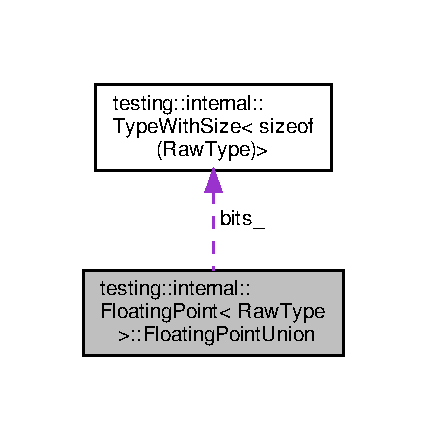
\includegraphics[width=205pt]{uniontesting_1_1internal_1_1FloatingPoint_1_1FloatingPointUnion__coll__graph}
\end{center}
\end{figure}
\subsection*{Public Attributes}
\begin{DoxyCompactItemize}
\item 
Raw\+Type \hyperlink{uniontesting_1_1internal_1_1FloatingPoint_1_1FloatingPointUnion_a4ee324889f70577721393e8e1920e4c6}{value\+\_\+}
\item 
\hyperlink{classtesting_1_1internal_1_1FloatingPoint_abf228bf6cd48f12c8b44c85b4971a731}{Bits} \hyperlink{uniontesting_1_1internal_1_1FloatingPoint_1_1FloatingPointUnion_aedb69e386f5d624a016f7a781302a2bf}{bits\+\_\+}
\end{DoxyCompactItemize}


\subsection{Member Data Documentation}
\mbox{\Hypertarget{uniontesting_1_1internal_1_1FloatingPoint_1_1FloatingPointUnion_aedb69e386f5d624a016f7a781302a2bf}\label{uniontesting_1_1internal_1_1FloatingPoint_1_1FloatingPointUnion_aedb69e386f5d624a016f7a781302a2bf}} 
\index{testing\+::internal\+::\+Floating\+Point\+::\+Floating\+Point\+Union@{testing\+::internal\+::\+Floating\+Point\+::\+Floating\+Point\+Union}!bits\+\_\+@{bits\+\_\+}}
\index{bits\+\_\+@{bits\+\_\+}!testing\+::internal\+::\+Floating\+Point\+::\+Floating\+Point\+Union@{testing\+::internal\+::\+Floating\+Point\+::\+Floating\+Point\+Union}}
\subsubsection{\texorpdfstring{bits\+\_\+}{bits\_}}
{\footnotesize\ttfamily template$<$typename Raw\+Type$>$ \\
\hyperlink{classtesting_1_1internal_1_1FloatingPoint_abf228bf6cd48f12c8b44c85b4971a731}{Bits} \hyperlink{classtesting_1_1internal_1_1FloatingPoint}{testing\+::internal\+::\+Floating\+Point}$<$ Raw\+Type $>$\+::Floating\+Point\+Union\+::bits\+\_\+}

\mbox{\Hypertarget{uniontesting_1_1internal_1_1FloatingPoint_1_1FloatingPointUnion_a4ee324889f70577721393e8e1920e4c6}\label{uniontesting_1_1internal_1_1FloatingPoint_1_1FloatingPointUnion_a4ee324889f70577721393e8e1920e4c6}} 
\index{testing\+::internal\+::\+Floating\+Point\+::\+Floating\+Point\+Union@{testing\+::internal\+::\+Floating\+Point\+::\+Floating\+Point\+Union}!value\+\_\+@{value\+\_\+}}
\index{value\+\_\+@{value\+\_\+}!testing\+::internal\+::\+Floating\+Point\+::\+Floating\+Point\+Union@{testing\+::internal\+::\+Floating\+Point\+::\+Floating\+Point\+Union}}
\subsubsection{\texorpdfstring{value\+\_\+}{value\_}}
{\footnotesize\ttfamily template$<$typename Raw\+Type$>$ \\
Raw\+Type \hyperlink{classtesting_1_1internal_1_1FloatingPoint}{testing\+::internal\+::\+Floating\+Point}$<$ Raw\+Type $>$\+::Floating\+Point\+Union\+::value\+\_\+}



The documentation for this union was generated from the following file\+:\begin{DoxyCompactItemize}
\item 
tests/googletest/include/gtest/internal/\hyperlink{gtest-internal_8h}{gtest-\/internal.\+h}\end{DoxyCompactItemize}

\hypertarget{classtesting_1_1internal_1_1FormatForComparison}{}\section{testing\+:\+:internal\+:\+:Format\+For\+Comparison$<$ To\+Print, Other\+Operand $>$ Class Template Reference}
\label{classtesting_1_1internal_1_1FormatForComparison}\index{testing\+::internal\+::\+Format\+For\+Comparison$<$ To\+Print, Other\+Operand $>$@{testing\+::internal\+::\+Format\+For\+Comparison$<$ To\+Print, Other\+Operand $>$}}


{\ttfamily \#include $<$gtest-\/printers.\+h$>$}

\subsection*{Static Public Member Functions}
\begin{DoxyCompactItemize}
\item 
\+::std\+::string \hyperlink{classtesting_1_1internal_1_1FormatForComparison_a2aeb688fc55b57abd3021d82eccad896}{Format} (const To\+Print \&value)
\end{DoxyCompactItemize}


\subsection{Member Function Documentation}
\mbox{\Hypertarget{classtesting_1_1internal_1_1FormatForComparison_a2aeb688fc55b57abd3021d82eccad896}\label{classtesting_1_1internal_1_1FormatForComparison_a2aeb688fc55b57abd3021d82eccad896}} 
\index{testing\+::internal\+::\+Format\+For\+Comparison@{testing\+::internal\+::\+Format\+For\+Comparison}!Format@{Format}}
\index{Format@{Format}!testing\+::internal\+::\+Format\+For\+Comparison@{testing\+::internal\+::\+Format\+For\+Comparison}}
\subsubsection{\texorpdfstring{Format()}{Format()}}
{\footnotesize\ttfamily template$<$typename To\+Print , typename Other\+Operand $>$ \\
\+::std\+::string \hyperlink{classtesting_1_1internal_1_1FormatForComparison}{testing\+::internal\+::\+Format\+For\+Comparison}$<$ To\+Print, Other\+Operand $>$\+::Format (\begin{DoxyParamCaption}\item[{const To\+Print \&}]{value }\end{DoxyParamCaption})\hspace{0.3cm}{\ttfamily [inline]}, {\ttfamily [static]}}



The documentation for this class was generated from the following file\+:\begin{DoxyCompactItemize}
\item 
tests/googletest/include/gtest/\hyperlink{gtest-printers_8h}{gtest-\/printers.\+h}\end{DoxyCompactItemize}

\hypertarget{classtesting_1_1internal_1_1FormatForComparison_3_01ToPrint[N]_00_01OtherOperand_01_4}{}\section{testing\+:\+:internal\+:\+:Format\+For\+Comparison$<$ To\+Print\mbox{[}N\mbox{]}, Other\+Operand $>$ Class Template Reference}
\label{classtesting_1_1internal_1_1FormatForComparison_3_01ToPrint[N]_00_01OtherOperand_01_4}\index{testing\+::internal\+::\+Format\+For\+Comparison$<$ To\+Print\mbox{[}N\mbox{]}, Other\+Operand $>$@{testing\+::internal\+::\+Format\+For\+Comparison$<$ To\+Print[N], Other\+Operand $>$}}


{\ttfamily \#include $<$gtest-\/printers.\+h$>$}

\subsection*{Static Public Member Functions}
\begin{DoxyCompactItemize}
\item 
\+::std\+::string \hyperlink{classtesting_1_1internal_1_1FormatForComparison_3_01ToPrint[N]_00_01OtherOperand_01_4_a76c526461c8fa7df75f7b32ab889b9e0}{Format} (const To\+Print $\ast$value)
\end{DoxyCompactItemize}


\subsection{Member Function Documentation}
\mbox{\Hypertarget{classtesting_1_1internal_1_1FormatForComparison_3_01ToPrint[N]_00_01OtherOperand_01_4_a76c526461c8fa7df75f7b32ab889b9e0}\label{classtesting_1_1internal_1_1FormatForComparison_3_01ToPrint[N]_00_01OtherOperand_01_4_a76c526461c8fa7df75f7b32ab889b9e0}} 
\index{testing\+::internal\+::\+Format\+For\+Comparison$<$ To\+Print\mbox{[}N\mbox{]}, Other\+Operand $>$@{testing\+::internal\+::\+Format\+For\+Comparison$<$ To\+Print[N], Other\+Operand $>$}!Format@{Format}}
\index{Format@{Format}!testing\+::internal\+::\+Format\+For\+Comparison$<$ To\+Print\mbox{[}N\mbox{]}, Other\+Operand $>$@{testing\+::internal\+::\+Format\+For\+Comparison$<$ To\+Print[N], Other\+Operand $>$}}
\subsubsection{\texorpdfstring{Format()}{Format()}}
{\footnotesize\ttfamily template$<$typename To\+Print , size\+\_\+t N, typename Other\+Operand $>$ \\
\+::std\+::string \hyperlink{classtesting_1_1internal_1_1FormatForComparison}{testing\+::internal\+::\+Format\+For\+Comparison}$<$ To\+Print\mbox{[}N\mbox{]}, Other\+Operand $>$\+::Format (\begin{DoxyParamCaption}\item[{const To\+Print $\ast$}]{value }\end{DoxyParamCaption})\hspace{0.3cm}{\ttfamily [inline]}, {\ttfamily [static]}}



The documentation for this class was generated from the following file\+:\begin{DoxyCompactItemize}
\item 
tests/googletest/include/gtest/\hyperlink{gtest-printers_8h}{gtest-\/printers.\+h}\end{DoxyCompactItemize}

\hypertarget{classtesting_1_1internal_1_1GTestLog}{}\section{testing\+:\+:internal\+:\+:G\+Test\+Log Class Reference}
\label{classtesting_1_1internal_1_1GTestLog}\index{testing\+::internal\+::\+G\+Test\+Log@{testing\+::internal\+::\+G\+Test\+Log}}


{\ttfamily \#include $<$gtest-\/port.\+h$>$}

\subsection*{Public Member Functions}
\begin{DoxyCompactItemize}
\item 
\hyperlink{classtesting_1_1internal_1_1GTestLog_a364691bf972983a59cfa2891062a64af}{G\+Test\+Log} (\hyperlink{namespacetesting_1_1internal_aa6255ef3b023c5b4e1a2198d887fb977}{G\+Test\+Log\+Severity} severity, const char $\ast$file, int line)
\item 
\hyperlink{classtesting_1_1internal_1_1GTestLog_a978a099703bbaa0f380216e8d7ee03d3}{$\sim$\+G\+Test\+Log} ()
\item 
\+::std\+::ostream \& \hyperlink{classtesting_1_1internal_1_1GTestLog_aebb92e67d98eca69f0347d5121dab27a}{Get\+Stream} ()
\end{DoxyCompactItemize}
\subsection*{Private Member Functions}
\begin{DoxyCompactItemize}
\item 
\hyperlink{classtesting_1_1internal_1_1GTestLog_ab6032a126d36a80163fdcd406fce3aad}{G\+T\+E\+S\+T\+\_\+\+D\+I\+S\+A\+L\+L\+O\+W\+\_\+\+C\+O\+P\+Y\+\_\+\+A\+N\+D\+\_\+\+A\+S\+S\+I\+G\+N\+\_\+} (\hyperlink{classtesting_1_1internal_1_1GTestLog}{G\+Test\+Log})
\end{DoxyCompactItemize}
\subsection*{Private Attributes}
\begin{DoxyCompactItemize}
\item 
const \hyperlink{namespacetesting_1_1internal_aa6255ef3b023c5b4e1a2198d887fb977}{G\+Test\+Log\+Severity} \hyperlink{classtesting_1_1internal_1_1GTestLog_ad8f75f5845900d0d2fd3cbb048a861be}{severity\+\_\+}
\end{DoxyCompactItemize}


\subsection{Constructor \& Destructor Documentation}
\mbox{\Hypertarget{classtesting_1_1internal_1_1GTestLog_a364691bf972983a59cfa2891062a64af}\label{classtesting_1_1internal_1_1GTestLog_a364691bf972983a59cfa2891062a64af}} 
\index{testing\+::internal\+::\+G\+Test\+Log@{testing\+::internal\+::\+G\+Test\+Log}!G\+Test\+Log@{G\+Test\+Log}}
\index{G\+Test\+Log@{G\+Test\+Log}!testing\+::internal\+::\+G\+Test\+Log@{testing\+::internal\+::\+G\+Test\+Log}}
\subsubsection{\texorpdfstring{G\+Test\+Log()}{GTestLog()}}
{\footnotesize\ttfamily testing\+::internal\+::\+G\+Test\+Log\+::\+G\+Test\+Log (\begin{DoxyParamCaption}\item[{\hyperlink{namespacetesting_1_1internal_aa6255ef3b023c5b4e1a2198d887fb977}{G\+Test\+Log\+Severity}}]{severity,  }\item[{const char $\ast$}]{file,  }\item[{int}]{line }\end{DoxyParamCaption})}

\mbox{\Hypertarget{classtesting_1_1internal_1_1GTestLog_a978a099703bbaa0f380216e8d7ee03d3}\label{classtesting_1_1internal_1_1GTestLog_a978a099703bbaa0f380216e8d7ee03d3}} 
\index{testing\+::internal\+::\+G\+Test\+Log@{testing\+::internal\+::\+G\+Test\+Log}!````~G\+Test\+Log@{$\sim$\+G\+Test\+Log}}
\index{````~G\+Test\+Log@{$\sim$\+G\+Test\+Log}!testing\+::internal\+::\+G\+Test\+Log@{testing\+::internal\+::\+G\+Test\+Log}}
\subsubsection{\texorpdfstring{$\sim$\+G\+Test\+Log()}{~GTestLog()}}
{\footnotesize\ttfamily testing\+::internal\+::\+G\+Test\+Log\+::$\sim$\+G\+Test\+Log (\begin{DoxyParamCaption}{ }\end{DoxyParamCaption})}



\subsection{Member Function Documentation}
\mbox{\Hypertarget{classtesting_1_1internal_1_1GTestLog_aebb92e67d98eca69f0347d5121dab27a}\label{classtesting_1_1internal_1_1GTestLog_aebb92e67d98eca69f0347d5121dab27a}} 
\index{testing\+::internal\+::\+G\+Test\+Log@{testing\+::internal\+::\+G\+Test\+Log}!Get\+Stream@{Get\+Stream}}
\index{Get\+Stream@{Get\+Stream}!testing\+::internal\+::\+G\+Test\+Log@{testing\+::internal\+::\+G\+Test\+Log}}
\subsubsection{\texorpdfstring{Get\+Stream()}{GetStream()}}
{\footnotesize\ttfamily \+::std\+::ostream\& testing\+::internal\+::\+G\+Test\+Log\+::\+Get\+Stream (\begin{DoxyParamCaption}{ }\end{DoxyParamCaption})\hspace{0.3cm}{\ttfamily [inline]}}

\mbox{\Hypertarget{classtesting_1_1internal_1_1GTestLog_ab6032a126d36a80163fdcd406fce3aad}\label{classtesting_1_1internal_1_1GTestLog_ab6032a126d36a80163fdcd406fce3aad}} 
\index{testing\+::internal\+::\+G\+Test\+Log@{testing\+::internal\+::\+G\+Test\+Log}!G\+T\+E\+S\+T\+\_\+\+D\+I\+S\+A\+L\+L\+O\+W\+\_\+\+C\+O\+P\+Y\+\_\+\+A\+N\+D\+\_\+\+A\+S\+S\+I\+G\+N\+\_\+@{G\+T\+E\+S\+T\+\_\+\+D\+I\+S\+A\+L\+L\+O\+W\+\_\+\+C\+O\+P\+Y\+\_\+\+A\+N\+D\+\_\+\+A\+S\+S\+I\+G\+N\+\_\+}}
\index{G\+T\+E\+S\+T\+\_\+\+D\+I\+S\+A\+L\+L\+O\+W\+\_\+\+C\+O\+P\+Y\+\_\+\+A\+N\+D\+\_\+\+A\+S\+S\+I\+G\+N\+\_\+@{G\+T\+E\+S\+T\+\_\+\+D\+I\+S\+A\+L\+L\+O\+W\+\_\+\+C\+O\+P\+Y\+\_\+\+A\+N\+D\+\_\+\+A\+S\+S\+I\+G\+N\+\_\+}!testing\+::internal\+::\+G\+Test\+Log@{testing\+::internal\+::\+G\+Test\+Log}}
\subsubsection{\texorpdfstring{G\+T\+E\+S\+T\+\_\+\+D\+I\+S\+A\+L\+L\+O\+W\+\_\+\+C\+O\+P\+Y\+\_\+\+A\+N\+D\+\_\+\+A\+S\+S\+I\+G\+N\+\_\+()}{GTEST\_DISALLOW\_COPY\_AND\_ASSIGN\_()}}
{\footnotesize\ttfamily testing\+::internal\+::\+G\+Test\+Log\+::\+G\+T\+E\+S\+T\+\_\+\+D\+I\+S\+A\+L\+L\+O\+W\+\_\+\+C\+O\+P\+Y\+\_\+\+A\+N\+D\+\_\+\+A\+S\+S\+I\+G\+N\+\_\+ (\begin{DoxyParamCaption}\item[{\hyperlink{classtesting_1_1internal_1_1GTestLog}{G\+Test\+Log}}]{ }\end{DoxyParamCaption})\hspace{0.3cm}{\ttfamily [private]}}



\subsection{Member Data Documentation}
\mbox{\Hypertarget{classtesting_1_1internal_1_1GTestLog_ad8f75f5845900d0d2fd3cbb048a861be}\label{classtesting_1_1internal_1_1GTestLog_ad8f75f5845900d0d2fd3cbb048a861be}} 
\index{testing\+::internal\+::\+G\+Test\+Log@{testing\+::internal\+::\+G\+Test\+Log}!severity\+\_\+@{severity\+\_\+}}
\index{severity\+\_\+@{severity\+\_\+}!testing\+::internal\+::\+G\+Test\+Log@{testing\+::internal\+::\+G\+Test\+Log}}
\subsubsection{\texorpdfstring{severity\+\_\+}{severity\_}}
{\footnotesize\ttfamily const \hyperlink{namespacetesting_1_1internal_aa6255ef3b023c5b4e1a2198d887fb977}{G\+Test\+Log\+Severity} testing\+::internal\+::\+G\+Test\+Log\+::severity\+\_\+\hspace{0.3cm}{\ttfamily [private]}}



The documentation for this class was generated from the following file\+:\begin{DoxyCompactItemize}
\item 
tests/googletest/include/gtest/internal/\hyperlink{gtest-port_8h}{gtest-\/port.\+h}\end{DoxyCompactItemize}

\hypertarget{classtesting_1_1internal_1_1GTestMutexLock}{}\section{testing\+:\+:internal\+:\+:G\+Test\+Mutex\+Lock Class Reference}
\label{classtesting_1_1internal_1_1GTestMutexLock}\index{testing\+::internal\+::\+G\+Test\+Mutex\+Lock@{testing\+::internal\+::\+G\+Test\+Mutex\+Lock}}


{\ttfamily \#include $<$gtest-\/port.\+h$>$}

\subsection*{Public Member Functions}
\begin{DoxyCompactItemize}
\item 
\hyperlink{classtesting_1_1internal_1_1GTestMutexLock_a77e3cba326d5356b4a1dea3790559c26}{G\+Test\+Mutex\+Lock} (\hyperlink{classtesting_1_1internal_1_1Mutex}{Mutex} $\ast$)
\end{DoxyCompactItemize}


\subsection{Constructor \& Destructor Documentation}
\mbox{\Hypertarget{classtesting_1_1internal_1_1GTestMutexLock_a77e3cba326d5356b4a1dea3790559c26}\label{classtesting_1_1internal_1_1GTestMutexLock_a77e3cba326d5356b4a1dea3790559c26}} 
\index{testing\+::internal\+::\+G\+Test\+Mutex\+Lock@{testing\+::internal\+::\+G\+Test\+Mutex\+Lock}!G\+Test\+Mutex\+Lock@{G\+Test\+Mutex\+Lock}}
\index{G\+Test\+Mutex\+Lock@{G\+Test\+Mutex\+Lock}!testing\+::internal\+::\+G\+Test\+Mutex\+Lock@{testing\+::internal\+::\+G\+Test\+Mutex\+Lock}}
\subsubsection{\texorpdfstring{G\+Test\+Mutex\+Lock()}{GTestMutexLock()}}
{\footnotesize\ttfamily testing\+::internal\+::\+G\+Test\+Mutex\+Lock\+::\+G\+Test\+Mutex\+Lock (\begin{DoxyParamCaption}\item[{\hyperlink{classtesting_1_1internal_1_1Mutex}{Mutex} $\ast$}]{ }\end{DoxyParamCaption})\hspace{0.3cm}{\ttfamily [inline]}, {\ttfamily [explicit]}}



The documentation for this class was generated from the following file\+:\begin{DoxyCompactItemize}
\item 
tests/googletest/include/gtest/internal/\hyperlink{gtest-port_8h}{gtest-\/port.\+h}\end{DoxyCompactItemize}

\hypertarget{classtesting_1_1internal_1_1IgnoredValue}{}\section{testing\+:\+:internal\+:\+:Ignored\+Value Class Reference}
\label{classtesting_1_1internal_1_1IgnoredValue}\index{testing\+::internal\+::\+Ignored\+Value@{testing\+::internal\+::\+Ignored\+Value}}


{\ttfamily \#include $<$gtest-\/internal.\+h$>$}

\subsection*{Classes}
\begin{DoxyCompactItemize}
\item 
struct \hyperlink{structtesting_1_1internal_1_1IgnoredValue_1_1Sink}{Sink}
\end{DoxyCompactItemize}
\subsection*{Public Member Functions}
\begin{DoxyCompactItemize}
\item 
{\footnotesize template$<$typename T , typename std\+::enable\+\_\+if$<$!std\+::is\+\_\+convertible$<$ T, Sink $>$\+::value, int $>$\+::type  = 0$>$ }\\\hyperlink{classtesting_1_1internal_1_1IgnoredValue_a851d14f6c0f584d5c5a49ddbc06d6538}{Ignored\+Value} (const T \&)
\end{DoxyCompactItemize}


\subsection{Constructor \& Destructor Documentation}
\mbox{\Hypertarget{classtesting_1_1internal_1_1IgnoredValue_a851d14f6c0f584d5c5a49ddbc06d6538}\label{classtesting_1_1internal_1_1IgnoredValue_a851d14f6c0f584d5c5a49ddbc06d6538}} 
\index{testing\+::internal\+::\+Ignored\+Value@{testing\+::internal\+::\+Ignored\+Value}!Ignored\+Value@{Ignored\+Value}}
\index{Ignored\+Value@{Ignored\+Value}!testing\+::internal\+::\+Ignored\+Value@{testing\+::internal\+::\+Ignored\+Value}}
\subsubsection{\texorpdfstring{Ignored\+Value()}{IgnoredValue()}}
{\footnotesize\ttfamily template$<$typename T , typename std\+::enable\+\_\+if$<$!std\+::is\+\_\+convertible$<$ T, Sink $>$\+::value, int $>$\+::type  = 0$>$ \\
testing\+::internal\+::\+Ignored\+Value\+::\+Ignored\+Value (\begin{DoxyParamCaption}\item[{const T \&}]{ }\end{DoxyParamCaption})\hspace{0.3cm}{\ttfamily [inline]}}



The documentation for this class was generated from the following file\+:\begin{DoxyCompactItemize}
\item 
tests/googletest/include/gtest/internal/\hyperlink{gtest-internal_8h}{gtest-\/internal.\+h}\end{DoxyCompactItemize}

\hypertarget{structtesting_1_1internal_1_1IndexSequence}{}\section{testing\+:\+:internal\+:\+:Index\+Sequence$<$ Is $>$ Struct Template Reference}
\label{structtesting_1_1internal_1_1IndexSequence}\index{testing\+::internal\+::\+Index\+Sequence$<$ Is $>$@{testing\+::internal\+::\+Index\+Sequence$<$ Is $>$}}


{\ttfamily \#include $<$gtest-\/internal.\+h$>$}

\subsection*{Public Types}
\begin{DoxyCompactItemize}
\item 
using \hyperlink{structtesting_1_1internal_1_1IndexSequence_a89bb13a7b5d169b69659f395dcec2b2d}{type} = \hyperlink{structtesting_1_1internal_1_1IndexSequence}{Index\+Sequence}
\end{DoxyCompactItemize}


\subsection{Member Typedef Documentation}
\mbox{\Hypertarget{structtesting_1_1internal_1_1IndexSequence_a89bb13a7b5d169b69659f395dcec2b2d}\label{structtesting_1_1internal_1_1IndexSequence_a89bb13a7b5d169b69659f395dcec2b2d}} 
\index{testing\+::internal\+::\+Index\+Sequence@{testing\+::internal\+::\+Index\+Sequence}!type@{type}}
\index{type@{type}!testing\+::internal\+::\+Index\+Sequence@{testing\+::internal\+::\+Index\+Sequence}}
\subsubsection{\texorpdfstring{type}{type}}
{\footnotesize\ttfamily template$<$size\+\_\+t... Is$>$ \\
using \hyperlink{structtesting_1_1internal_1_1IndexSequence}{testing\+::internal\+::\+Index\+Sequence}$<$ Is $>$\+::\hyperlink{structtesting_1_1internal_1_1IndexSequence_a89bb13a7b5d169b69659f395dcec2b2d}{type} =  \hyperlink{structtesting_1_1internal_1_1IndexSequence}{Index\+Sequence}}



The documentation for this struct was generated from the following file\+:\begin{DoxyCompactItemize}
\item 
tests/googletest/include/gtest/internal/\hyperlink{gtest-internal_8h}{gtest-\/internal.\+h}\end{DoxyCompactItemize}

\hypertarget{structtesting_1_1internal_1_1ParameterizedTestSuiteInfo_1_1InstantiationInfo}{}\section{testing\+:\+:internal\+:\+:Parameterized\+Test\+Suite\+Info$<$ Test\+Suite $>$\+:\+:Instantiation\+Info Struct Reference}
\label{structtesting_1_1internal_1_1ParameterizedTestSuiteInfo_1_1InstantiationInfo}\index{testing\+::internal\+::\+Parameterized\+Test\+Suite\+Info$<$ Test\+Suite $>$\+::\+Instantiation\+Info@{testing\+::internal\+::\+Parameterized\+Test\+Suite\+Info$<$ Test\+Suite $>$\+::\+Instantiation\+Info}}
\subsection*{Public Member Functions}
\begin{DoxyCompactItemize}
\item 
\hyperlink{structtesting_1_1internal_1_1ParameterizedTestSuiteInfo_1_1InstantiationInfo_a1cde67cef70758ca16047040747e19c0}{Instantiation\+Info} (const std\+::string \&name\+\_\+in, Generator\+Creation\+Func $\ast$generator\+\_\+in, \hyperlink{classtesting_1_1internal_1_1ParameterizedTestSuiteInfo_a3b4f232b7d6d3df941bb8e81b6b534a4}{Param\+Name\+Generator\+Func} $\ast$name\+\_\+func\+\_\+in, const char $\ast$file\+\_\+in, int line\+\_\+in)
\end{DoxyCompactItemize}
\subsection*{Public Attributes}
\begin{DoxyCompactItemize}
\item 
std\+::string \hyperlink{structtesting_1_1internal_1_1ParameterizedTestSuiteInfo_1_1InstantiationInfo_a7e66a4d302537389c8c8efcc9acbe826}{name}
\item 
Generator\+Creation\+Func $\ast$ \hyperlink{structtesting_1_1internal_1_1ParameterizedTestSuiteInfo_1_1InstantiationInfo_a98306e8a0d25571d84821206d79629cf}{generator}
\item 
\hyperlink{classtesting_1_1internal_1_1ParameterizedTestSuiteInfo_a3b4f232b7d6d3df941bb8e81b6b534a4}{Param\+Name\+Generator\+Func} $\ast$ \hyperlink{structtesting_1_1internal_1_1ParameterizedTestSuiteInfo_1_1InstantiationInfo_a754244a7055f2d8c83b1b5e1656afe5f}{name\+\_\+func}
\item 
const char $\ast$ \hyperlink{structtesting_1_1internal_1_1ParameterizedTestSuiteInfo_1_1InstantiationInfo_ab9cb66c639c2af3dbb30afe4cf56256c}{file}
\item 
int \hyperlink{structtesting_1_1internal_1_1ParameterizedTestSuiteInfo_1_1InstantiationInfo_a95d4b9adfe5d42f66cc12214f434fa0d}{line}
\end{DoxyCompactItemize}


\subsection{Constructor \& Destructor Documentation}
\mbox{\Hypertarget{structtesting_1_1internal_1_1ParameterizedTestSuiteInfo_1_1InstantiationInfo_a1cde67cef70758ca16047040747e19c0}\label{structtesting_1_1internal_1_1ParameterizedTestSuiteInfo_1_1InstantiationInfo_a1cde67cef70758ca16047040747e19c0}} 
\index{testing\+::internal\+::\+Parameterized\+Test\+Suite\+Info\+::\+Instantiation\+Info@{testing\+::internal\+::\+Parameterized\+Test\+Suite\+Info\+::\+Instantiation\+Info}!Instantiation\+Info@{Instantiation\+Info}}
\index{Instantiation\+Info@{Instantiation\+Info}!testing\+::internal\+::\+Parameterized\+Test\+Suite\+Info\+::\+Instantiation\+Info@{testing\+::internal\+::\+Parameterized\+Test\+Suite\+Info\+::\+Instantiation\+Info}}
\subsubsection{\texorpdfstring{Instantiation\+Info()}{InstantiationInfo()}}
{\footnotesize\ttfamily template$<$class Test\+Suite$>$ \\
\hyperlink{classtesting_1_1internal_1_1ParameterizedTestSuiteInfo}{testing\+::internal\+::\+Parameterized\+Test\+Suite\+Info}$<$ \hyperlink{classtesting_1_1TestSuite}{Test\+Suite} $>$\+::Instantiation\+Info\+::\+Instantiation\+Info (\begin{DoxyParamCaption}\item[{const std\+::string \&}]{name\+\_\+in,  }\item[{Generator\+Creation\+Func $\ast$}]{generator\+\_\+in,  }\item[{\hyperlink{classtesting_1_1internal_1_1ParameterizedTestSuiteInfo_a3b4f232b7d6d3df941bb8e81b6b534a4}{Param\+Name\+Generator\+Func} $\ast$}]{name\+\_\+func\+\_\+in,  }\item[{const char $\ast$}]{file\+\_\+in,  }\item[{int}]{line\+\_\+in }\end{DoxyParamCaption})\hspace{0.3cm}{\ttfamily [inline]}}



\subsection{Member Data Documentation}
\mbox{\Hypertarget{structtesting_1_1internal_1_1ParameterizedTestSuiteInfo_1_1InstantiationInfo_ab9cb66c639c2af3dbb30afe4cf56256c}\label{structtesting_1_1internal_1_1ParameterizedTestSuiteInfo_1_1InstantiationInfo_ab9cb66c639c2af3dbb30afe4cf56256c}} 
\index{testing\+::internal\+::\+Parameterized\+Test\+Suite\+Info\+::\+Instantiation\+Info@{testing\+::internal\+::\+Parameterized\+Test\+Suite\+Info\+::\+Instantiation\+Info}!file@{file}}
\index{file@{file}!testing\+::internal\+::\+Parameterized\+Test\+Suite\+Info\+::\+Instantiation\+Info@{testing\+::internal\+::\+Parameterized\+Test\+Suite\+Info\+::\+Instantiation\+Info}}
\subsubsection{\texorpdfstring{file}{file}}
{\footnotesize\ttfamily template$<$class Test\+Suite$>$ \\
const char$\ast$ \hyperlink{classtesting_1_1internal_1_1ParameterizedTestSuiteInfo}{testing\+::internal\+::\+Parameterized\+Test\+Suite\+Info}$<$ \hyperlink{classtesting_1_1TestSuite}{Test\+Suite} $>$\+::Instantiation\+Info\+::file}

\mbox{\Hypertarget{structtesting_1_1internal_1_1ParameterizedTestSuiteInfo_1_1InstantiationInfo_a98306e8a0d25571d84821206d79629cf}\label{structtesting_1_1internal_1_1ParameterizedTestSuiteInfo_1_1InstantiationInfo_a98306e8a0d25571d84821206d79629cf}} 
\index{testing\+::internal\+::\+Parameterized\+Test\+Suite\+Info\+::\+Instantiation\+Info@{testing\+::internal\+::\+Parameterized\+Test\+Suite\+Info\+::\+Instantiation\+Info}!generator@{generator}}
\index{generator@{generator}!testing\+::internal\+::\+Parameterized\+Test\+Suite\+Info\+::\+Instantiation\+Info@{testing\+::internal\+::\+Parameterized\+Test\+Suite\+Info\+::\+Instantiation\+Info}}
\subsubsection{\texorpdfstring{generator}{generator}}
{\footnotesize\ttfamily template$<$class Test\+Suite$>$ \\
Generator\+Creation\+Func$\ast$ \hyperlink{classtesting_1_1internal_1_1ParameterizedTestSuiteInfo}{testing\+::internal\+::\+Parameterized\+Test\+Suite\+Info}$<$ \hyperlink{classtesting_1_1TestSuite}{Test\+Suite} $>$\+::Instantiation\+Info\+::generator}

\mbox{\Hypertarget{structtesting_1_1internal_1_1ParameterizedTestSuiteInfo_1_1InstantiationInfo_a95d4b9adfe5d42f66cc12214f434fa0d}\label{structtesting_1_1internal_1_1ParameterizedTestSuiteInfo_1_1InstantiationInfo_a95d4b9adfe5d42f66cc12214f434fa0d}} 
\index{testing\+::internal\+::\+Parameterized\+Test\+Suite\+Info\+::\+Instantiation\+Info@{testing\+::internal\+::\+Parameterized\+Test\+Suite\+Info\+::\+Instantiation\+Info}!line@{line}}
\index{line@{line}!testing\+::internal\+::\+Parameterized\+Test\+Suite\+Info\+::\+Instantiation\+Info@{testing\+::internal\+::\+Parameterized\+Test\+Suite\+Info\+::\+Instantiation\+Info}}
\subsubsection{\texorpdfstring{line}{line}}
{\footnotesize\ttfamily template$<$class Test\+Suite$>$ \\
int \hyperlink{classtesting_1_1internal_1_1ParameterizedTestSuiteInfo}{testing\+::internal\+::\+Parameterized\+Test\+Suite\+Info}$<$ \hyperlink{classtesting_1_1TestSuite}{Test\+Suite} $>$\+::Instantiation\+Info\+::line}

\mbox{\Hypertarget{structtesting_1_1internal_1_1ParameterizedTestSuiteInfo_1_1InstantiationInfo_a7e66a4d302537389c8c8efcc9acbe826}\label{structtesting_1_1internal_1_1ParameterizedTestSuiteInfo_1_1InstantiationInfo_a7e66a4d302537389c8c8efcc9acbe826}} 
\index{testing\+::internal\+::\+Parameterized\+Test\+Suite\+Info\+::\+Instantiation\+Info@{testing\+::internal\+::\+Parameterized\+Test\+Suite\+Info\+::\+Instantiation\+Info}!name@{name}}
\index{name@{name}!testing\+::internal\+::\+Parameterized\+Test\+Suite\+Info\+::\+Instantiation\+Info@{testing\+::internal\+::\+Parameterized\+Test\+Suite\+Info\+::\+Instantiation\+Info}}
\subsubsection{\texorpdfstring{name}{name}}
{\footnotesize\ttfamily template$<$class Test\+Suite$>$ \\
std\+::string \hyperlink{classtesting_1_1internal_1_1ParameterizedTestSuiteInfo}{testing\+::internal\+::\+Parameterized\+Test\+Suite\+Info}$<$ \hyperlink{classtesting_1_1TestSuite}{Test\+Suite} $>$\+::Instantiation\+Info\+::name}

\mbox{\Hypertarget{structtesting_1_1internal_1_1ParameterizedTestSuiteInfo_1_1InstantiationInfo_a754244a7055f2d8c83b1b5e1656afe5f}\label{structtesting_1_1internal_1_1ParameterizedTestSuiteInfo_1_1InstantiationInfo_a754244a7055f2d8c83b1b5e1656afe5f}} 
\index{testing\+::internal\+::\+Parameterized\+Test\+Suite\+Info\+::\+Instantiation\+Info@{testing\+::internal\+::\+Parameterized\+Test\+Suite\+Info\+::\+Instantiation\+Info}!name\+\_\+func@{name\+\_\+func}}
\index{name\+\_\+func@{name\+\_\+func}!testing\+::internal\+::\+Parameterized\+Test\+Suite\+Info\+::\+Instantiation\+Info@{testing\+::internal\+::\+Parameterized\+Test\+Suite\+Info\+::\+Instantiation\+Info}}
\subsubsection{\texorpdfstring{name\+\_\+func}{name\_func}}
{\footnotesize\ttfamily template$<$class Test\+Suite$>$ \\
\hyperlink{classtesting_1_1internal_1_1ParameterizedTestSuiteInfo_a3b4f232b7d6d3df941bb8e81b6b534a4}{Param\+Name\+Generator\+Func}$\ast$ \hyperlink{classtesting_1_1internal_1_1ParameterizedTestSuiteInfo}{testing\+::internal\+::\+Parameterized\+Test\+Suite\+Info}$<$ \hyperlink{classtesting_1_1TestSuite}{Test\+Suite} $>$\+::Instantiation\+Info\+::name\+\_\+func}



The documentation for this struct was generated from the following file\+:\begin{DoxyCompactItemize}
\item 
tests/googletest/include/gtest/internal/\hyperlink{gtest-param-util_8h}{gtest-\/param-\/util.\+h}\end{DoxyCompactItemize}

\hypertarget{classInstantiationInMultipleTranslationUnitsTest}{}\section{Instantiation\+In\+Multiple\+Translation\+Units\+Test Class Reference}
\label{classInstantiationInMultipleTranslationUnitsTest}\index{Instantiation\+In\+Multiple\+Translation\+Units\+Test@{Instantiation\+In\+Multiple\+Translation\+Units\+Test}}


{\ttfamily \#include $<$googletest-\/param-\/test-\/test.\+h$>$}



Inheritance diagram for Instantiation\+In\+Multiple\+Translation\+Units\+Test\+:\nopagebreak
\begin{figure}[H]
\begin{center}
\leavevmode
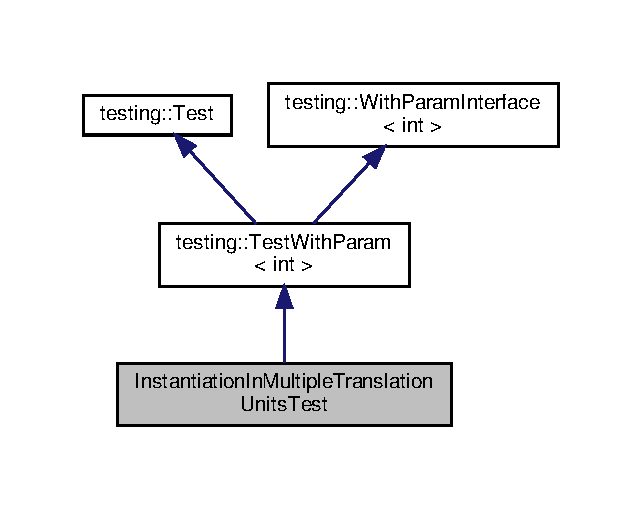
\includegraphics[width=308pt]{classInstantiationInMultipleTranslationUnitsTest__inherit__graph}
\end{center}
\end{figure}


Collaboration diagram for Instantiation\+In\+Multiple\+Translation\+Units\+Test\+:\nopagebreak
\begin{figure}[H]
\begin{center}
\leavevmode
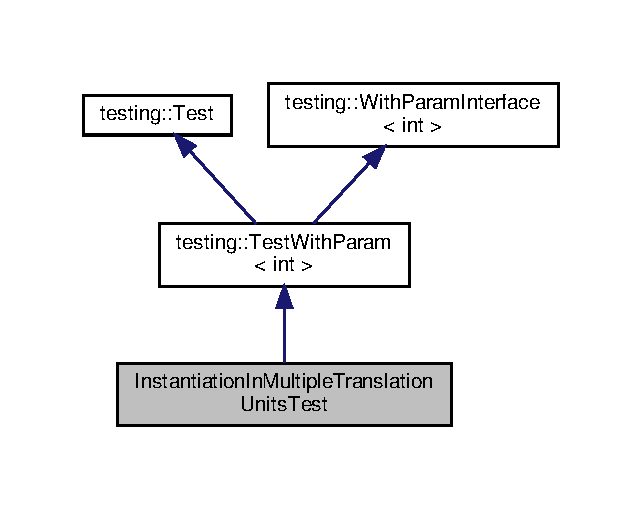
\includegraphics[width=308pt]{classInstantiationInMultipleTranslationUnitsTest__coll__graph}
\end{center}
\end{figure}
\subsection*{Additional Inherited Members}


The documentation for this class was generated from the following file\+:\begin{DoxyCompactItemize}
\item 
tests/googletest/test/\hyperlink{googletest-param-test-test_8h}{googletest-\/param-\/test-\/test.\+h}\end{DoxyCompactItemize}

\hypertarget{structtesting_1_1internal_1_1is__same}{}\section{testing\+:\+:internal\+:\+:is\+\_\+same$<$ T, U $>$ Struct Template Reference}
\label{structtesting_1_1internal_1_1is__same}\index{testing\+::internal\+::is\+\_\+same$<$ T, U $>$@{testing\+::internal\+::is\+\_\+same$<$ T, U $>$}}


{\ttfamily \#include $<$gtest-\/port.\+h$>$}



Inheritance diagram for testing\+:\+:internal\+:\+:is\+\_\+same$<$ T, U $>$\+:\nopagebreak
\begin{figure}[H]
\begin{center}
\leavevmode
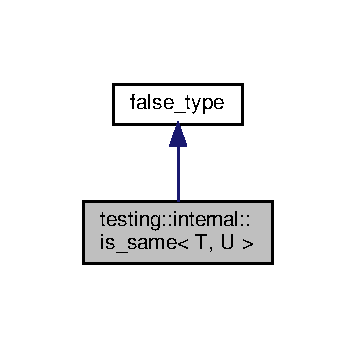
\includegraphics[width=171pt]{structtesting_1_1internal_1_1is__same__inherit__graph}
\end{center}
\end{figure}


Collaboration diagram for testing\+:\+:internal\+:\+:is\+\_\+same$<$ T, U $>$\+:\nopagebreak
\begin{figure}[H]
\begin{center}
\leavevmode
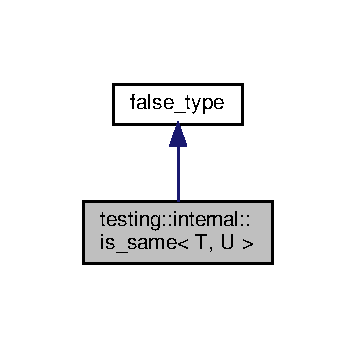
\includegraphics[width=171pt]{structtesting_1_1internal_1_1is__same__coll__graph}
\end{center}
\end{figure}
\subsection*{Additional Inherited Members}


The documentation for this struct was generated from the following file\+:\begin{DoxyCompactItemize}
\item 
tests/googletest/include/gtest/internal/\hyperlink{gtest-port_8h}{gtest-\/port.\+h}\end{DoxyCompactItemize}

\hypertarget{structtesting_1_1internal_1_1is__same_3_01T_00_01T_01_4}{}\section{testing\+:\+:internal\+:\+:is\+\_\+same$<$ T, T $>$ Struct Template Reference}
\label{structtesting_1_1internal_1_1is__same_3_01T_00_01T_01_4}\index{testing\+::internal\+::is\+\_\+same$<$ T, T $>$@{testing\+::internal\+::is\+\_\+same$<$ T, T $>$}}


{\ttfamily \#include $<$gtest-\/port.\+h$>$}



Inheritance diagram for testing\+:\+:internal\+:\+:is\+\_\+same$<$ T, T $>$\+:\nopagebreak
\begin{figure}[H]
\begin{center}
\leavevmode
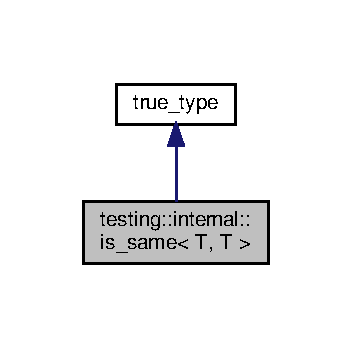
\includegraphics[width=169pt]{structtesting_1_1internal_1_1is__same_3_01T_00_01T_01_4__inherit__graph}
\end{center}
\end{figure}


Collaboration diagram for testing\+:\+:internal\+:\+:is\+\_\+same$<$ T, T $>$\+:\nopagebreak
\begin{figure}[H]
\begin{center}
\leavevmode
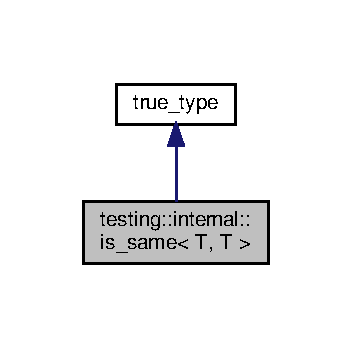
\includegraphics[width=169pt]{structtesting_1_1internal_1_1is__same_3_01T_00_01T_01_4__coll__graph}
\end{center}
\end{figure}
\subsection*{Additional Inherited Members}


The documentation for this struct was generated from the following file\+:\begin{DoxyCompactItemize}
\item 
tests/googletest/include/gtest/internal/\hyperlink{gtest-port_8h}{gtest-\/port.\+h}\end{DoxyCompactItemize}

\hypertarget{structtesting_1_1internal_1_1IsAProtocolMessage}{}\section{testing\+:\+:internal\+:\+:Is\+A\+Protocol\+Message$<$ T $>$ Struct Template Reference}
\label{structtesting_1_1internal_1_1IsAProtocolMessage}\index{testing\+::internal\+::\+Is\+A\+Protocol\+Message$<$ T $>$@{testing\+::internal\+::\+Is\+A\+Protocol\+Message$<$ T $>$}}


{\ttfamily \#include $<$gtest-\/internal.\+h$>$}



Inheritance diagram for testing\+:\+:internal\+:\+:Is\+A\+Protocol\+Message$<$ T $>$\+:\nopagebreak
\begin{figure}[H]
\begin{center}
\leavevmode
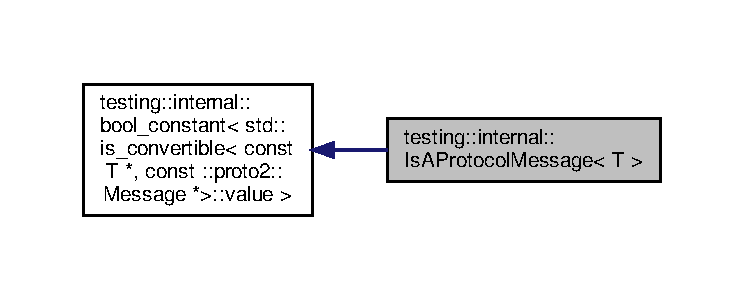
\includegraphics[width=350pt]{structtesting_1_1internal_1_1IsAProtocolMessage__inherit__graph}
\end{center}
\end{figure}


Collaboration diagram for testing\+:\+:internal\+:\+:Is\+A\+Protocol\+Message$<$ T $>$\+:\nopagebreak
\begin{figure}[H]
\begin{center}
\leavevmode
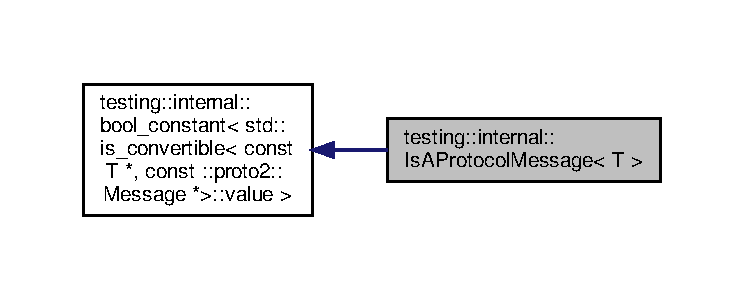
\includegraphics[width=350pt]{structtesting_1_1internal_1_1IsAProtocolMessage__coll__graph}
\end{center}
\end{figure}
\subsection*{Additional Inherited Members}


The documentation for this struct was generated from the following file\+:\begin{DoxyCompactItemize}
\item 
tests/googletest/include/gtest/internal/\hyperlink{gtest-internal_8h}{gtest-\/internal.\+h}\end{DoxyCompactItemize}

\hypertarget{structtesting_1_1internal_1_1IsHashTable}{}\section{testing\+:\+:internal\+:\+:Is\+Hash\+Table$<$ T $>$ Struct Template Reference}
\label{structtesting_1_1internal_1_1IsHashTable}\index{testing\+::internal\+::\+Is\+Hash\+Table$<$ T $>$@{testing\+::internal\+::\+Is\+Hash\+Table$<$ T $>$}}


{\ttfamily \#include $<$gtest-\/internal.\+h$>$}

\subsection*{Static Public Attributes}
\begin{DoxyCompactItemize}
\item 
static const bool \hyperlink{structtesting_1_1internal_1_1IsHashTable_a165e0a3eddfa5fadf9b950be6432d848}{value} = sizeof(\hyperlink{structtesting_1_1internal_1_1IsHashTable_acc4d1e2307a1e0527932da7a7d354f06}{test}$<$T$>$(nullptr, nullptr)) == sizeof(int)
\end{DoxyCompactItemize}
\subsection*{Static Private Member Functions}
\begin{DoxyCompactItemize}
\item 
{\footnotesize template$<$typename U $>$ }\\static char \hyperlink{structtesting_1_1internal_1_1IsHashTable_acc4d1e2307a1e0527932da7a7d354f06}{test} (typename U\+::hasher $\ast$, typename U\+::reverse\+\_\+iterator $\ast$)
\item 
{\footnotesize template$<$typename U $>$ }\\static int \hyperlink{structtesting_1_1internal_1_1IsHashTable_a195b49a6ae5090b6266a5fa4ab771962}{test} (typename U\+::hasher $\ast$,...)
\item 
{\footnotesize template$<$typename U $>$ }\\static char \hyperlink{structtesting_1_1internal_1_1IsHashTable_a40461295b959ff31e06241d4de072be0}{test} (...)
\end{DoxyCompactItemize}


\subsection{Member Function Documentation}
\mbox{\Hypertarget{structtesting_1_1internal_1_1IsHashTable_acc4d1e2307a1e0527932da7a7d354f06}\label{structtesting_1_1internal_1_1IsHashTable_acc4d1e2307a1e0527932da7a7d354f06}} 
\index{testing\+::internal\+::\+Is\+Hash\+Table@{testing\+::internal\+::\+Is\+Hash\+Table}!test@{test}}
\index{test@{test}!testing\+::internal\+::\+Is\+Hash\+Table@{testing\+::internal\+::\+Is\+Hash\+Table}}
\subsubsection{\texorpdfstring{test()}{test()}\hspace{0.1cm}{\footnotesize\ttfamily [1/3]}}
{\footnotesize\ttfamily template$<$typename T $>$ \\
template$<$typename U $>$ \\
static char \hyperlink{structtesting_1_1internal_1_1IsHashTable}{testing\+::internal\+::\+Is\+Hash\+Table}$<$ T $>$\+::test (\begin{DoxyParamCaption}\item[{typename U\+::hasher $\ast$}]{,  }\item[{typename U\+::reverse\+\_\+iterator $\ast$}]{ }\end{DoxyParamCaption})\hspace{0.3cm}{\ttfamily [static]}, {\ttfamily [private]}}

\mbox{\Hypertarget{structtesting_1_1internal_1_1IsHashTable_a195b49a6ae5090b6266a5fa4ab771962}\label{structtesting_1_1internal_1_1IsHashTable_a195b49a6ae5090b6266a5fa4ab771962}} 
\index{testing\+::internal\+::\+Is\+Hash\+Table@{testing\+::internal\+::\+Is\+Hash\+Table}!test@{test}}
\index{test@{test}!testing\+::internal\+::\+Is\+Hash\+Table@{testing\+::internal\+::\+Is\+Hash\+Table}}
\subsubsection{\texorpdfstring{test()}{test()}\hspace{0.1cm}{\footnotesize\ttfamily [2/3]}}
{\footnotesize\ttfamily template$<$typename T $>$ \\
template$<$typename U $>$ \\
static int \hyperlink{structtesting_1_1internal_1_1IsHashTable}{testing\+::internal\+::\+Is\+Hash\+Table}$<$ T $>$\+::test (\begin{DoxyParamCaption}\item[{typename U\+::hasher $\ast$}]{,  }\item[{}]{... }\end{DoxyParamCaption})\hspace{0.3cm}{\ttfamily [static]}, {\ttfamily [private]}}

\mbox{\Hypertarget{structtesting_1_1internal_1_1IsHashTable_a40461295b959ff31e06241d4de072be0}\label{structtesting_1_1internal_1_1IsHashTable_a40461295b959ff31e06241d4de072be0}} 
\index{testing\+::internal\+::\+Is\+Hash\+Table@{testing\+::internal\+::\+Is\+Hash\+Table}!test@{test}}
\index{test@{test}!testing\+::internal\+::\+Is\+Hash\+Table@{testing\+::internal\+::\+Is\+Hash\+Table}}
\subsubsection{\texorpdfstring{test()}{test()}\hspace{0.1cm}{\footnotesize\ttfamily [3/3]}}
{\footnotesize\ttfamily template$<$typename T $>$ \\
template$<$typename U $>$ \\
static char \hyperlink{structtesting_1_1internal_1_1IsHashTable}{testing\+::internal\+::\+Is\+Hash\+Table}$<$ T $>$\+::test (\begin{DoxyParamCaption}\item[{}]{... }\end{DoxyParamCaption})\hspace{0.3cm}{\ttfamily [static]}, {\ttfamily [private]}}



\subsection{Member Data Documentation}
\mbox{\Hypertarget{structtesting_1_1internal_1_1IsHashTable_a165e0a3eddfa5fadf9b950be6432d848}\label{structtesting_1_1internal_1_1IsHashTable_a165e0a3eddfa5fadf9b950be6432d848}} 
\index{testing\+::internal\+::\+Is\+Hash\+Table@{testing\+::internal\+::\+Is\+Hash\+Table}!value@{value}}
\index{value@{value}!testing\+::internal\+::\+Is\+Hash\+Table@{testing\+::internal\+::\+Is\+Hash\+Table}}
\subsubsection{\texorpdfstring{value}{value}}
{\footnotesize\ttfamily template$<$typename T $>$ \\
const bool \hyperlink{structtesting_1_1internal_1_1IsHashTable}{testing\+::internal\+::\+Is\+Hash\+Table}$<$ T $>$\+::value = sizeof(\hyperlink{structtesting_1_1internal_1_1IsHashTable_acc4d1e2307a1e0527932da7a7d354f06}{test}$<$T$>$(nullptr, nullptr)) == sizeof(int)\hspace{0.3cm}{\ttfamily [static]}}



The documentation for this struct was generated from the following file\+:\begin{DoxyCompactItemize}
\item 
tests/googletest/include/gtest/internal/\hyperlink{gtest-internal_8h}{gtest-\/internal.\+h}\end{DoxyCompactItemize}

\hypertarget{structtesting_1_1internal_1_1IsRecursiveContainer}{}\section{testing\+:\+:internal\+:\+:Is\+Recursive\+Container$<$ C $>$ Struct Template Reference}
\label{structtesting_1_1internal_1_1IsRecursiveContainer}\index{testing\+::internal\+::\+Is\+Recursive\+Container$<$ C $>$@{testing\+::internal\+::\+Is\+Recursive\+Container$<$ C $>$}}


{\ttfamily \#include $<$gtest-\/internal.\+h$>$}



Inheritance diagram for testing\+:\+:internal\+:\+:Is\+Recursive\+Container$<$ C $>$\+:\nopagebreak
\begin{figure}[H]
\begin{center}
\leavevmode
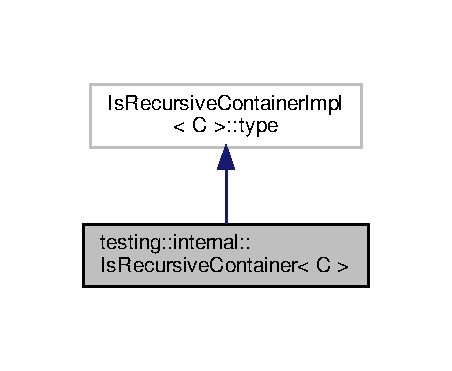
\includegraphics[width=217pt]{structtesting_1_1internal_1_1IsRecursiveContainer__inherit__graph}
\end{center}
\end{figure}


Collaboration diagram for testing\+:\+:internal\+:\+:Is\+Recursive\+Container$<$ C $>$\+:\nopagebreak
\begin{figure}[H]
\begin{center}
\leavevmode
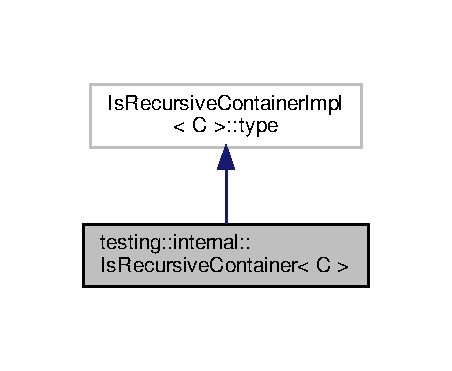
\includegraphics[width=217pt]{structtesting_1_1internal_1_1IsRecursiveContainer__coll__graph}
\end{center}
\end{figure}


The documentation for this struct was generated from the following file\+:\begin{DoxyCompactItemize}
\item 
tests/googletest/include/gtest/internal/\hyperlink{gtest-internal_8h}{gtest-\/internal.\+h}\end{DoxyCompactItemize}

\hypertarget{structtesting_1_1internal_1_1IsRecursiveContainerImpl}{}\section{testing\+:\+:internal\+:\+:Is\+Recursive\+Container\+Impl$<$ C, bool $>$ Struct Template Reference}
\label{structtesting_1_1internal_1_1IsRecursiveContainerImpl}\index{testing\+::internal\+::\+Is\+Recursive\+Container\+Impl$<$ C, bool $>$@{testing\+::internal\+::\+Is\+Recursive\+Container\+Impl$<$ C, bool $>$}}


{\ttfamily \#include $<$gtest-\/internal.\+h$>$}



The documentation for this struct was generated from the following file\+:\begin{DoxyCompactItemize}
\item 
tests/googletest/include/gtest/internal/\hyperlink{gtest-internal_8h}{gtest-\/internal.\+h}\end{DoxyCompactItemize}

\hypertarget{structtesting_1_1internal_1_1IsRecursiveContainerImpl_3_01C_00_01false_01_4}{}\section{testing\+:\+:internal\+:\+:Is\+Recursive\+Container\+Impl$<$ C, false $>$ Struct Template Reference}
\label{structtesting_1_1internal_1_1IsRecursiveContainerImpl_3_01C_00_01false_01_4}\index{testing\+::internal\+::\+Is\+Recursive\+Container\+Impl$<$ C, false $>$@{testing\+::internal\+::\+Is\+Recursive\+Container\+Impl$<$ C, false $>$}}


{\ttfamily \#include $<$gtest-\/internal.\+h$>$}



Inheritance diagram for testing\+:\+:internal\+:\+:Is\+Recursive\+Container\+Impl$<$ C, false $>$\+:\nopagebreak
\begin{figure}[H]
\begin{center}
\leavevmode
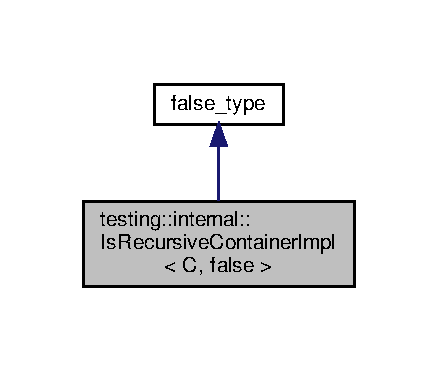
\includegraphics[width=210pt]{structtesting_1_1internal_1_1IsRecursiveContainerImpl_3_01C_00_01false_01_4__inherit__graph}
\end{center}
\end{figure}


Collaboration diagram for testing\+:\+:internal\+:\+:Is\+Recursive\+Container\+Impl$<$ C, false $>$\+:\nopagebreak
\begin{figure}[H]
\begin{center}
\leavevmode
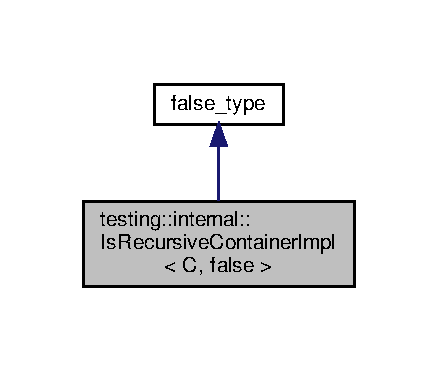
\includegraphics[width=210pt]{structtesting_1_1internal_1_1IsRecursiveContainerImpl_3_01C_00_01false_01_4__coll__graph}
\end{center}
\end{figure}
\subsection*{Additional Inherited Members}


The documentation for this struct was generated from the following file\+:\begin{DoxyCompactItemize}
\item 
tests/googletest/include/gtest/internal/\hyperlink{gtest-internal_8h}{gtest-\/internal.\+h}\end{DoxyCompactItemize}

\hypertarget{structtesting_1_1internal_1_1IsRecursiveContainerImpl_3_01C_00_01true_01_4}{}\section{testing\+:\+:internal\+:\+:Is\+Recursive\+Container\+Impl$<$ C, true $>$ Struct Template Reference}
\label{structtesting_1_1internal_1_1IsRecursiveContainerImpl_3_01C_00_01true_01_4}\index{testing\+::internal\+::\+Is\+Recursive\+Container\+Impl$<$ C, true $>$@{testing\+::internal\+::\+Is\+Recursive\+Container\+Impl$<$ C, true $>$}}


{\ttfamily \#include $<$gtest-\/internal.\+h$>$}

\subsection*{Public Types}
\begin{DoxyCompactItemize}
\item 
using \hyperlink{structtesting_1_1internal_1_1IsRecursiveContainerImpl_3_01C_00_01true_01_4_a5e8e2cf58f0d2581e9e3ab5f5630cd61}{value\+\_\+type} = decltype($\ast$std\+::declval$<$ typename C\+::const\+\_\+iterator $>$())
\item 
using \hyperlink{structtesting_1_1internal_1_1IsRecursiveContainerImpl_3_01C_00_01true_01_4_a24b611fbe1b9a7c524ee54ae01324388}{type} = \hyperlink{structtesting_1_1internal_1_1is__same}{is\+\_\+same}$<$ typename std\+::remove\+\_\+const$<$ typename std\+::remove\+\_\+reference$<$ \hyperlink{structtesting_1_1internal_1_1IsRecursiveContainerImpl_3_01C_00_01true_01_4_a5e8e2cf58f0d2581e9e3ab5f5630cd61}{value\+\_\+type} $>$\+::\hyperlink{structtesting_1_1internal_1_1IsRecursiveContainerImpl_3_01C_00_01true_01_4_a24b611fbe1b9a7c524ee54ae01324388}{type} $>$\+::\hyperlink{structtesting_1_1internal_1_1IsRecursiveContainerImpl_3_01C_00_01true_01_4_a24b611fbe1b9a7c524ee54ae01324388}{type}, C $>$
\end{DoxyCompactItemize}


\subsection{Member Typedef Documentation}
\mbox{\Hypertarget{structtesting_1_1internal_1_1IsRecursiveContainerImpl_3_01C_00_01true_01_4_a24b611fbe1b9a7c524ee54ae01324388}\label{structtesting_1_1internal_1_1IsRecursiveContainerImpl_3_01C_00_01true_01_4_a24b611fbe1b9a7c524ee54ae01324388}} 
\index{testing\+::internal\+::\+Is\+Recursive\+Container\+Impl$<$ C, true $>$@{testing\+::internal\+::\+Is\+Recursive\+Container\+Impl$<$ C, true $>$}!type@{type}}
\index{type@{type}!testing\+::internal\+::\+Is\+Recursive\+Container\+Impl$<$ C, true $>$@{testing\+::internal\+::\+Is\+Recursive\+Container\+Impl$<$ C, true $>$}}
\subsubsection{\texorpdfstring{type}{type}}
{\footnotesize\ttfamily template$<$typename C $>$ \\
using \hyperlink{structtesting_1_1internal_1_1IsRecursiveContainerImpl}{testing\+::internal\+::\+Is\+Recursive\+Container\+Impl}$<$ C, true $>$\+::\hyperlink{structtesting_1_1internal_1_1IsRecursiveContainerImpl_3_01C_00_01true_01_4_a24b611fbe1b9a7c524ee54ae01324388}{type} =  \hyperlink{structtesting_1_1internal_1_1is__same}{is\+\_\+same}$<$typename std\+::remove\+\_\+const$<$ typename std\+::remove\+\_\+reference$<$\hyperlink{structtesting_1_1internal_1_1IsRecursiveContainerImpl_3_01C_00_01true_01_4_a5e8e2cf58f0d2581e9e3ab5f5630cd61}{value\+\_\+type}$>$\+::\hyperlink{structtesting_1_1internal_1_1IsRecursiveContainerImpl_3_01C_00_01true_01_4_a24b611fbe1b9a7c524ee54ae01324388}{type}$>$\+::\hyperlink{structtesting_1_1internal_1_1IsRecursiveContainerImpl_3_01C_00_01true_01_4_a24b611fbe1b9a7c524ee54ae01324388}{type}, C$>$}

\mbox{\Hypertarget{structtesting_1_1internal_1_1IsRecursiveContainerImpl_3_01C_00_01true_01_4_a5e8e2cf58f0d2581e9e3ab5f5630cd61}\label{structtesting_1_1internal_1_1IsRecursiveContainerImpl_3_01C_00_01true_01_4_a5e8e2cf58f0d2581e9e3ab5f5630cd61}} 
\index{testing\+::internal\+::\+Is\+Recursive\+Container\+Impl$<$ C, true $>$@{testing\+::internal\+::\+Is\+Recursive\+Container\+Impl$<$ C, true $>$}!value\+\_\+type@{value\+\_\+type}}
\index{value\+\_\+type@{value\+\_\+type}!testing\+::internal\+::\+Is\+Recursive\+Container\+Impl$<$ C, true $>$@{testing\+::internal\+::\+Is\+Recursive\+Container\+Impl$<$ C, true $>$}}
\subsubsection{\texorpdfstring{value\+\_\+type}{value\_type}}
{\footnotesize\ttfamily template$<$typename C $>$ \\
using \hyperlink{structtesting_1_1internal_1_1IsRecursiveContainerImpl}{testing\+::internal\+::\+Is\+Recursive\+Container\+Impl}$<$ C, true $>$\+::\hyperlink{structtesting_1_1internal_1_1IsRecursiveContainerImpl_3_01C_00_01true_01_4_a5e8e2cf58f0d2581e9e3ab5f5630cd61}{value\+\_\+type} =  decltype($\ast$std\+::declval$<$typename C\+::const\+\_\+iterator$>$())}



The documentation for this struct was generated from the following file\+:\begin{DoxyCompactItemize}
\item 
tests/googletest/include/gtest/internal/\hyperlink{gtest-internal_8h}{gtest-\/internal.\+h}\end{DoxyCompactItemize}

\hypertarget{structtesting_1_1internal_1_1IsSame}{}\section{testing\+:\+:internal\+:\+:Is\+Same$<$ T, U $>$ Struct Template Reference}
\label{structtesting_1_1internal_1_1IsSame}\index{testing\+::internal\+::\+Is\+Same$<$ T, U $>$@{testing\+::internal\+::\+Is\+Same$<$ T, U $>$}}


{\ttfamily \#include $<$gtest-\/port.\+h$>$}

\subsection*{Public Types}
\begin{DoxyCompactItemize}
\item 
enum \{ \hyperlink{structtesting_1_1internal_1_1IsSame_acebf1dabd866eb05f295125a4991d9baa58968a8c680eff4326a25fab55aa0a5e}{value} = false
 \}
\end{DoxyCompactItemize}


\subsection{Member Enumeration Documentation}
\mbox{\Hypertarget{structtesting_1_1internal_1_1IsSame_acebf1dabd866eb05f295125a4991d9ba}\label{structtesting_1_1internal_1_1IsSame_acebf1dabd866eb05f295125a4991d9ba}} 
\subsubsection{\texorpdfstring{anonymous enum}{anonymous enum}}
{\footnotesize\ttfamily template$<$typename T , typename U $>$ \\
anonymous enum}

\begin{DoxyEnumFields}{Enumerator}
\raisebox{\heightof{T}}[0pt][0pt]{\index{value@{value}!testing\+::internal\+::\+Is\+Same@{testing\+::internal\+::\+Is\+Same}}\index{testing\+::internal\+::\+Is\+Same@{testing\+::internal\+::\+Is\+Same}!value@{value}}}\mbox{\Hypertarget{structtesting_1_1internal_1_1IsSame_acebf1dabd866eb05f295125a4991d9baa58968a8c680eff4326a25fab55aa0a5e}\label{structtesting_1_1internal_1_1IsSame_acebf1dabd866eb05f295125a4991d9baa58968a8c680eff4326a25fab55aa0a5e}} 
value&\\
\hline

\end{DoxyEnumFields}


The documentation for this struct was generated from the following file\+:\begin{DoxyCompactItemize}
\item 
tests/googletest/include/gtest/internal/\hyperlink{gtest-port_8h}{gtest-\/port.\+h}\end{DoxyCompactItemize}

\hypertarget{structtesting_1_1internal_1_1IsSame_3_01T_00_01T_01_4}{}\section{testing\+:\+:internal\+:\+:Is\+Same$<$ T, T $>$ Struct Template Reference}
\label{structtesting_1_1internal_1_1IsSame_3_01T_00_01T_01_4}\index{testing\+::internal\+::\+Is\+Same$<$ T, T $>$@{testing\+::internal\+::\+Is\+Same$<$ T, T $>$}}


{\ttfamily \#include $<$gtest-\/port.\+h$>$}

\subsection*{Public Types}
\begin{DoxyCompactItemize}
\item 
enum \{ \hyperlink{structtesting_1_1internal_1_1IsSame_3_01T_00_01T_01_4_a4f43bdb63adfd73e0a8cace4cc6368dea0bb1c61b491e4e13216a3f9e9cd24c69}{value} = true
 \}
\end{DoxyCompactItemize}


\subsection{Member Enumeration Documentation}
\mbox{\Hypertarget{structtesting_1_1internal_1_1IsSame_3_01T_00_01T_01_4_a4f43bdb63adfd73e0a8cace4cc6368de}\label{structtesting_1_1internal_1_1IsSame_3_01T_00_01T_01_4_a4f43bdb63adfd73e0a8cace4cc6368de}} 
\subsubsection{\texorpdfstring{anonymous enum}{anonymous enum}}
{\footnotesize\ttfamily template$<$typename T $>$ \\
anonymous enum}

\begin{DoxyEnumFields}{Enumerator}
\raisebox{\heightof{T}}[0pt][0pt]{\index{value@{value}!testing\+::internal\+::\+Is\+Same$<$ T, T $>$@{testing\+::internal\+::\+Is\+Same$<$ T, T $>$}}\index{testing\+::internal\+::\+Is\+Same$<$ T, T $>$@{testing\+::internal\+::\+Is\+Same$<$ T, T $>$}!value@{value}}}\mbox{\Hypertarget{structtesting_1_1internal_1_1IsSame_3_01T_00_01T_01_4_a4f43bdb63adfd73e0a8cace4cc6368dea0bb1c61b491e4e13216a3f9e9cd24c69}\label{structtesting_1_1internal_1_1IsSame_3_01T_00_01T_01_4_a4f43bdb63adfd73e0a8cace4cc6368dea0bb1c61b491e4e13216a3f9e9cd24c69}} 
value&\\
\hline

\end{DoxyEnumFields}


The documentation for this struct was generated from the following file\+:\begin{DoxyCompactItemize}
\item 
tests/googletest/include/gtest/internal/\hyperlink{gtest-port_8h}{gtest-\/port.\+h}\end{DoxyCompactItemize}

\hypertarget{classtesting_1_1internal_1_1RangeGenerator_1_1Iterator}{}\section{testing\+:\+:internal\+:\+:Range\+Generator$<$ T, IncrementT $>$\+:\+:Iterator Class Reference}
\label{classtesting_1_1internal_1_1RangeGenerator_1_1Iterator}\index{testing\+::internal\+::\+Range\+Generator$<$ T, Increment\+T $>$\+::\+Iterator@{testing\+::internal\+::\+Range\+Generator$<$ T, Increment\+T $>$\+::\+Iterator}}


Inheritance diagram for testing\+:\+:internal\+:\+:Range\+Generator$<$ T, IncrementT $>$\+:\+:Iterator\+:\nopagebreak
\begin{figure}[H]
\begin{center}
\leavevmode
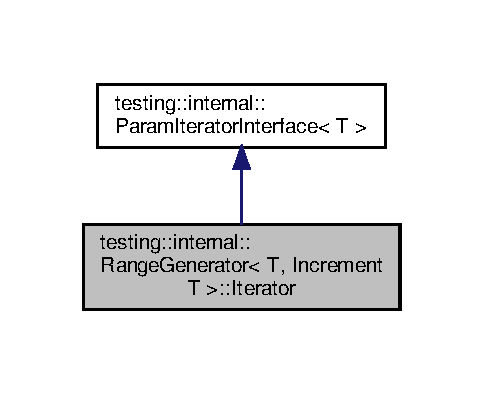
\includegraphics[width=232pt]{classtesting_1_1internal_1_1RangeGenerator_1_1Iterator__inherit__graph}
\end{center}
\end{figure}


Collaboration diagram for testing\+:\+:internal\+:\+:Range\+Generator$<$ T, IncrementT $>$\+:\+:Iterator\+:\nopagebreak
\begin{figure}[H]
\begin{center}
\leavevmode
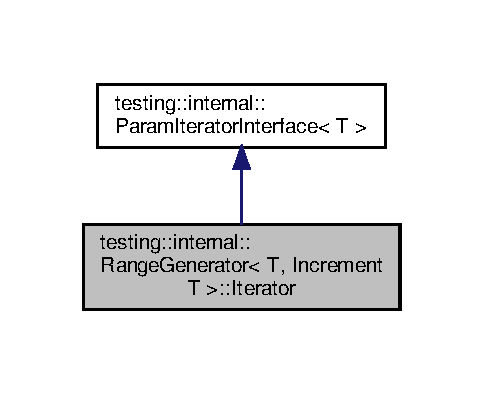
\includegraphics[width=232pt]{classtesting_1_1internal_1_1RangeGenerator_1_1Iterator__coll__graph}
\end{center}
\end{figure}
\subsection*{Public Member Functions}
\begin{DoxyCompactItemize}
\item 
\hyperlink{classtesting_1_1internal_1_1RangeGenerator_1_1Iterator_a960184d2ea0ff223d9cf4d6ab015baa8}{Iterator} (const \hyperlink{classtesting_1_1internal_1_1ParamGeneratorInterface}{Param\+Generator\+Interface}$<$ T $>$ $\ast$base, T value, int index, IncrementT step)
\item 
\hyperlink{classtesting_1_1internal_1_1RangeGenerator_1_1Iterator_a09f0f9f1d40f7a3d04e4e82f7274b2ab}{$\sim$\+Iterator} () override
\item 
const \hyperlink{classtesting_1_1internal_1_1ParamGeneratorInterface}{Param\+Generator\+Interface}$<$ T $>$ $\ast$ \hyperlink{classtesting_1_1internal_1_1RangeGenerator_1_1Iterator_aa1dc4151e1eed1c546059ecb4f72440b}{Base\+Generator} () const override
\item 
void \hyperlink{classtesting_1_1internal_1_1RangeGenerator_1_1Iterator_ad17bd99e352c43b8ab654a4ad479d06e}{Advance} () override
\item 
\hyperlink{classtesting_1_1internal_1_1ParamIteratorInterface}{Param\+Iterator\+Interface}$<$ T $>$ $\ast$ \hyperlink{classtesting_1_1internal_1_1RangeGenerator_1_1Iterator_a61a764294b66272d730f5ff5e0acdcf4}{Clone} () const override
\item 
const T $\ast$ \hyperlink{classtesting_1_1internal_1_1RangeGenerator_1_1Iterator_acbdfc5919d37fb9514914afb041e50ff}{Current} () const override
\item 
bool \hyperlink{classtesting_1_1internal_1_1RangeGenerator_1_1Iterator_a534406abbddb137d7672c2b53d5bff0b}{Equals} (const \hyperlink{classtesting_1_1internal_1_1ParamIteratorInterface}{Param\+Iterator\+Interface}$<$ T $>$ \&other) const override
\end{DoxyCompactItemize}
\subsection*{Private Member Functions}
\begin{DoxyCompactItemize}
\item 
\hyperlink{classtesting_1_1internal_1_1RangeGenerator_1_1Iterator_a14150df56c79ae26f1beaea1e7548ebc}{Iterator} (const \hyperlink{classtesting_1_1internal_1_1RangeGenerator_1_1Iterator}{Iterator} \&other)
\item 
void \hyperlink{classtesting_1_1internal_1_1RangeGenerator_1_1Iterator_acd95aafca4a92db473dd4a88bbc9ab1b}{operator=} (const \hyperlink{classtesting_1_1internal_1_1RangeGenerator_1_1Iterator}{Iterator} \&other)
\end{DoxyCompactItemize}
\subsection*{Private Attributes}
\begin{DoxyCompactItemize}
\item 
const \hyperlink{classtesting_1_1internal_1_1ParamGeneratorInterface}{Param\+Generator\+Interface}$<$ T $>$ $\ast$const \hyperlink{classtesting_1_1internal_1_1RangeGenerator_1_1Iterator_aa6767ad52e3cbd87c457fb5b8b6a21d9}{base\+\_\+}
\item 
T \hyperlink{classtesting_1_1internal_1_1RangeGenerator_1_1Iterator_aab59a7070669d64348494a1fb1795934}{value\+\_\+}
\item 
int \hyperlink{classtesting_1_1internal_1_1RangeGenerator_1_1Iterator_a2e9064f8da43367550e82eea8adabc2c}{index\+\_\+}
\item 
const IncrementT \hyperlink{classtesting_1_1internal_1_1RangeGenerator_1_1Iterator_a18ebb51d061695f102c2ef74cade8618}{step\+\_\+}
\end{DoxyCompactItemize}


\subsection{Constructor \& Destructor Documentation}
\mbox{\Hypertarget{classtesting_1_1internal_1_1RangeGenerator_1_1Iterator_a960184d2ea0ff223d9cf4d6ab015baa8}\label{classtesting_1_1internal_1_1RangeGenerator_1_1Iterator_a960184d2ea0ff223d9cf4d6ab015baa8}} 
\index{testing\+::internal\+::\+Range\+Generator\+::\+Iterator@{testing\+::internal\+::\+Range\+Generator\+::\+Iterator}!Iterator@{Iterator}}
\index{Iterator@{Iterator}!testing\+::internal\+::\+Range\+Generator\+::\+Iterator@{testing\+::internal\+::\+Range\+Generator\+::\+Iterator}}
\subsubsection{\texorpdfstring{Iterator()}{Iterator()}\hspace{0.1cm}{\footnotesize\ttfamily [1/2]}}
{\footnotesize\ttfamily template$<$typename T , typename IncrementT $>$ \\
\hyperlink{classtesting_1_1internal_1_1RangeGenerator}{testing\+::internal\+::\+Range\+Generator}$<$ T, IncrementT $>$\+::Iterator\+::\+Iterator (\begin{DoxyParamCaption}\item[{const \hyperlink{classtesting_1_1internal_1_1ParamGeneratorInterface}{Param\+Generator\+Interface}$<$ T $>$ $\ast$}]{base,  }\item[{T}]{value,  }\item[{int}]{index,  }\item[{IncrementT}]{step }\end{DoxyParamCaption})\hspace{0.3cm}{\ttfamily [inline]}}

\mbox{\Hypertarget{classtesting_1_1internal_1_1RangeGenerator_1_1Iterator_a09f0f9f1d40f7a3d04e4e82f7274b2ab}\label{classtesting_1_1internal_1_1RangeGenerator_1_1Iterator_a09f0f9f1d40f7a3d04e4e82f7274b2ab}} 
\index{testing\+::internal\+::\+Range\+Generator\+::\+Iterator@{testing\+::internal\+::\+Range\+Generator\+::\+Iterator}!````~Iterator@{$\sim$\+Iterator}}
\index{````~Iterator@{$\sim$\+Iterator}!testing\+::internal\+::\+Range\+Generator\+::\+Iterator@{testing\+::internal\+::\+Range\+Generator\+::\+Iterator}}
\subsubsection{\texorpdfstring{$\sim$\+Iterator()}{~Iterator()}}
{\footnotesize\ttfamily template$<$typename T , typename IncrementT $>$ \\
\hyperlink{classtesting_1_1internal_1_1RangeGenerator}{testing\+::internal\+::\+Range\+Generator}$<$ T, IncrementT $>$\+::Iterator\+::$\sim$\+Iterator (\begin{DoxyParamCaption}{ }\end{DoxyParamCaption})\hspace{0.3cm}{\ttfamily [inline]}, {\ttfamily [override]}}

\mbox{\Hypertarget{classtesting_1_1internal_1_1RangeGenerator_1_1Iterator_a14150df56c79ae26f1beaea1e7548ebc}\label{classtesting_1_1internal_1_1RangeGenerator_1_1Iterator_a14150df56c79ae26f1beaea1e7548ebc}} 
\index{testing\+::internal\+::\+Range\+Generator\+::\+Iterator@{testing\+::internal\+::\+Range\+Generator\+::\+Iterator}!Iterator@{Iterator}}
\index{Iterator@{Iterator}!testing\+::internal\+::\+Range\+Generator\+::\+Iterator@{testing\+::internal\+::\+Range\+Generator\+::\+Iterator}}
\subsubsection{\texorpdfstring{Iterator()}{Iterator()}\hspace{0.1cm}{\footnotesize\ttfamily [2/2]}}
{\footnotesize\ttfamily template$<$typename T , typename IncrementT $>$ \\
\hyperlink{classtesting_1_1internal_1_1RangeGenerator}{testing\+::internal\+::\+Range\+Generator}$<$ T, IncrementT $>$\+::Iterator\+::\+Iterator (\begin{DoxyParamCaption}\item[{const \hyperlink{classtesting_1_1internal_1_1RangeGenerator_1_1Iterator}{Iterator} \&}]{other }\end{DoxyParamCaption})\hspace{0.3cm}{\ttfamily [inline]}, {\ttfamily [private]}}



\subsection{Member Function Documentation}
\mbox{\Hypertarget{classtesting_1_1internal_1_1RangeGenerator_1_1Iterator_ad17bd99e352c43b8ab654a4ad479d06e}\label{classtesting_1_1internal_1_1RangeGenerator_1_1Iterator_ad17bd99e352c43b8ab654a4ad479d06e}} 
\index{testing\+::internal\+::\+Range\+Generator\+::\+Iterator@{testing\+::internal\+::\+Range\+Generator\+::\+Iterator}!Advance@{Advance}}
\index{Advance@{Advance}!testing\+::internal\+::\+Range\+Generator\+::\+Iterator@{testing\+::internal\+::\+Range\+Generator\+::\+Iterator}}
\subsubsection{\texorpdfstring{Advance()}{Advance()}}
{\footnotesize\ttfamily template$<$typename T , typename IncrementT $>$ \\
void \hyperlink{classtesting_1_1internal_1_1RangeGenerator}{testing\+::internal\+::\+Range\+Generator}$<$ T, IncrementT $>$\+::Iterator\+::\+Advance (\begin{DoxyParamCaption}{ }\end{DoxyParamCaption})\hspace{0.3cm}{\ttfamily [inline]}, {\ttfamily [override]}, {\ttfamily [virtual]}}



Implements \hyperlink{classtesting_1_1internal_1_1ParamIteratorInterface_a600dbd35fcb551463e379516a1abea48}{testing\+::internal\+::\+Param\+Iterator\+Interface$<$ T $>$}.

\mbox{\Hypertarget{classtesting_1_1internal_1_1RangeGenerator_1_1Iterator_aa1dc4151e1eed1c546059ecb4f72440b}\label{classtesting_1_1internal_1_1RangeGenerator_1_1Iterator_aa1dc4151e1eed1c546059ecb4f72440b}} 
\index{testing\+::internal\+::\+Range\+Generator\+::\+Iterator@{testing\+::internal\+::\+Range\+Generator\+::\+Iterator}!Base\+Generator@{Base\+Generator}}
\index{Base\+Generator@{Base\+Generator}!testing\+::internal\+::\+Range\+Generator\+::\+Iterator@{testing\+::internal\+::\+Range\+Generator\+::\+Iterator}}
\subsubsection{\texorpdfstring{Base\+Generator()}{BaseGenerator()}}
{\footnotesize\ttfamily template$<$typename T , typename IncrementT $>$ \\
const \hyperlink{classtesting_1_1internal_1_1ParamGeneratorInterface}{Param\+Generator\+Interface}$<$T$>$$\ast$ \hyperlink{classtesting_1_1internal_1_1RangeGenerator}{testing\+::internal\+::\+Range\+Generator}$<$ T, IncrementT $>$\+::Iterator\+::\+Base\+Generator (\begin{DoxyParamCaption}{ }\end{DoxyParamCaption}) const\hspace{0.3cm}{\ttfamily [inline]}, {\ttfamily [override]}, {\ttfamily [virtual]}}



Implements \hyperlink{classtesting_1_1internal_1_1ParamIteratorInterface_a17500953df75ecda1ace46c08ff731e9}{testing\+::internal\+::\+Param\+Iterator\+Interface$<$ T $>$}.

\mbox{\Hypertarget{classtesting_1_1internal_1_1RangeGenerator_1_1Iterator_a61a764294b66272d730f5ff5e0acdcf4}\label{classtesting_1_1internal_1_1RangeGenerator_1_1Iterator_a61a764294b66272d730f5ff5e0acdcf4}} 
\index{testing\+::internal\+::\+Range\+Generator\+::\+Iterator@{testing\+::internal\+::\+Range\+Generator\+::\+Iterator}!Clone@{Clone}}
\index{Clone@{Clone}!testing\+::internal\+::\+Range\+Generator\+::\+Iterator@{testing\+::internal\+::\+Range\+Generator\+::\+Iterator}}
\subsubsection{\texorpdfstring{Clone()}{Clone()}}
{\footnotesize\ttfamily template$<$typename T , typename IncrementT $>$ \\
\hyperlink{classtesting_1_1internal_1_1ParamIteratorInterface}{Param\+Iterator\+Interface}$<$T$>$$\ast$ \hyperlink{classtesting_1_1internal_1_1RangeGenerator}{testing\+::internal\+::\+Range\+Generator}$<$ T, IncrementT $>$\+::Iterator\+::\+Clone (\begin{DoxyParamCaption}{ }\end{DoxyParamCaption}) const\hspace{0.3cm}{\ttfamily [inline]}, {\ttfamily [override]}, {\ttfamily [virtual]}}



Implements \hyperlink{classtesting_1_1internal_1_1ParamIteratorInterface_a4998c23e27e2943d97546011aa35db80}{testing\+::internal\+::\+Param\+Iterator\+Interface$<$ T $>$}.

\mbox{\Hypertarget{classtesting_1_1internal_1_1RangeGenerator_1_1Iterator_acbdfc5919d37fb9514914afb041e50ff}\label{classtesting_1_1internal_1_1RangeGenerator_1_1Iterator_acbdfc5919d37fb9514914afb041e50ff}} 
\index{testing\+::internal\+::\+Range\+Generator\+::\+Iterator@{testing\+::internal\+::\+Range\+Generator\+::\+Iterator}!Current@{Current}}
\index{Current@{Current}!testing\+::internal\+::\+Range\+Generator\+::\+Iterator@{testing\+::internal\+::\+Range\+Generator\+::\+Iterator}}
\subsubsection{\texorpdfstring{Current()}{Current()}}
{\footnotesize\ttfamily template$<$typename T , typename IncrementT $>$ \\
const T$\ast$ \hyperlink{classtesting_1_1internal_1_1RangeGenerator}{testing\+::internal\+::\+Range\+Generator}$<$ T, IncrementT $>$\+::Iterator\+::\+Current (\begin{DoxyParamCaption}{ }\end{DoxyParamCaption}) const\hspace{0.3cm}{\ttfamily [inline]}, {\ttfamily [override]}, {\ttfamily [virtual]}}



Implements \hyperlink{classtesting_1_1internal_1_1ParamIteratorInterface_adfff808576d929085679c315b255af7e}{testing\+::internal\+::\+Param\+Iterator\+Interface$<$ T $>$}.

\mbox{\Hypertarget{classtesting_1_1internal_1_1RangeGenerator_1_1Iterator_a534406abbddb137d7672c2b53d5bff0b}\label{classtesting_1_1internal_1_1RangeGenerator_1_1Iterator_a534406abbddb137d7672c2b53d5bff0b}} 
\index{testing\+::internal\+::\+Range\+Generator\+::\+Iterator@{testing\+::internal\+::\+Range\+Generator\+::\+Iterator}!Equals@{Equals}}
\index{Equals@{Equals}!testing\+::internal\+::\+Range\+Generator\+::\+Iterator@{testing\+::internal\+::\+Range\+Generator\+::\+Iterator}}
\subsubsection{\texorpdfstring{Equals()}{Equals()}}
{\footnotesize\ttfamily template$<$typename T , typename IncrementT $>$ \\
bool \hyperlink{classtesting_1_1internal_1_1RangeGenerator}{testing\+::internal\+::\+Range\+Generator}$<$ T, IncrementT $>$\+::Iterator\+::\+Equals (\begin{DoxyParamCaption}\item[{const \hyperlink{classtesting_1_1internal_1_1ParamIteratorInterface}{Param\+Iterator\+Interface}$<$ T $>$ \&}]{other }\end{DoxyParamCaption}) const\hspace{0.3cm}{\ttfamily [inline]}, {\ttfamily [override]}, {\ttfamily [virtual]}}



Implements \hyperlink{classtesting_1_1internal_1_1ParamIteratorInterface_a9d811697a752d46f7bd6a0082f9040a3}{testing\+::internal\+::\+Param\+Iterator\+Interface$<$ T $>$}.

\mbox{\Hypertarget{classtesting_1_1internal_1_1RangeGenerator_1_1Iterator_acd95aafca4a92db473dd4a88bbc9ab1b}\label{classtesting_1_1internal_1_1RangeGenerator_1_1Iterator_acd95aafca4a92db473dd4a88bbc9ab1b}} 
\index{testing\+::internal\+::\+Range\+Generator\+::\+Iterator@{testing\+::internal\+::\+Range\+Generator\+::\+Iterator}!operator=@{operator=}}
\index{operator=@{operator=}!testing\+::internal\+::\+Range\+Generator\+::\+Iterator@{testing\+::internal\+::\+Range\+Generator\+::\+Iterator}}
\subsubsection{\texorpdfstring{operator=()}{operator=()}}
{\footnotesize\ttfamily template$<$typename T , typename IncrementT $>$ \\
void \hyperlink{classtesting_1_1internal_1_1RangeGenerator}{testing\+::internal\+::\+Range\+Generator}$<$ T, IncrementT $>$\+::Iterator\+::operator= (\begin{DoxyParamCaption}\item[{const \hyperlink{classtesting_1_1internal_1_1RangeGenerator_1_1Iterator}{Iterator} \&}]{other }\end{DoxyParamCaption})\hspace{0.3cm}{\ttfamily [private]}}



\subsection{Member Data Documentation}
\mbox{\Hypertarget{classtesting_1_1internal_1_1RangeGenerator_1_1Iterator_aa6767ad52e3cbd87c457fb5b8b6a21d9}\label{classtesting_1_1internal_1_1RangeGenerator_1_1Iterator_aa6767ad52e3cbd87c457fb5b8b6a21d9}} 
\index{testing\+::internal\+::\+Range\+Generator\+::\+Iterator@{testing\+::internal\+::\+Range\+Generator\+::\+Iterator}!base\+\_\+@{base\+\_\+}}
\index{base\+\_\+@{base\+\_\+}!testing\+::internal\+::\+Range\+Generator\+::\+Iterator@{testing\+::internal\+::\+Range\+Generator\+::\+Iterator}}
\subsubsection{\texorpdfstring{base\+\_\+}{base\_}}
{\footnotesize\ttfamily template$<$typename T , typename IncrementT $>$ \\
const \hyperlink{classtesting_1_1internal_1_1ParamGeneratorInterface}{Param\+Generator\+Interface}$<$T$>$$\ast$ const \hyperlink{classtesting_1_1internal_1_1RangeGenerator}{testing\+::internal\+::\+Range\+Generator}$<$ T, IncrementT $>$\+::Iterator\+::base\+\_\+\hspace{0.3cm}{\ttfamily [private]}}

\mbox{\Hypertarget{classtesting_1_1internal_1_1RangeGenerator_1_1Iterator_a2e9064f8da43367550e82eea8adabc2c}\label{classtesting_1_1internal_1_1RangeGenerator_1_1Iterator_a2e9064f8da43367550e82eea8adabc2c}} 
\index{testing\+::internal\+::\+Range\+Generator\+::\+Iterator@{testing\+::internal\+::\+Range\+Generator\+::\+Iterator}!index\+\_\+@{index\+\_\+}}
\index{index\+\_\+@{index\+\_\+}!testing\+::internal\+::\+Range\+Generator\+::\+Iterator@{testing\+::internal\+::\+Range\+Generator\+::\+Iterator}}
\subsubsection{\texorpdfstring{index\+\_\+}{index\_}}
{\footnotesize\ttfamily template$<$typename T , typename IncrementT $>$ \\
int \hyperlink{classtesting_1_1internal_1_1RangeGenerator}{testing\+::internal\+::\+Range\+Generator}$<$ T, IncrementT $>$\+::Iterator\+::index\+\_\+\hspace{0.3cm}{\ttfamily [private]}}

\mbox{\Hypertarget{classtesting_1_1internal_1_1RangeGenerator_1_1Iterator_a18ebb51d061695f102c2ef74cade8618}\label{classtesting_1_1internal_1_1RangeGenerator_1_1Iterator_a18ebb51d061695f102c2ef74cade8618}} 
\index{testing\+::internal\+::\+Range\+Generator\+::\+Iterator@{testing\+::internal\+::\+Range\+Generator\+::\+Iterator}!step\+\_\+@{step\+\_\+}}
\index{step\+\_\+@{step\+\_\+}!testing\+::internal\+::\+Range\+Generator\+::\+Iterator@{testing\+::internal\+::\+Range\+Generator\+::\+Iterator}}
\subsubsection{\texorpdfstring{step\+\_\+}{step\_}}
{\footnotesize\ttfamily template$<$typename T , typename IncrementT $>$ \\
const IncrementT \hyperlink{classtesting_1_1internal_1_1RangeGenerator}{testing\+::internal\+::\+Range\+Generator}$<$ T, IncrementT $>$\+::Iterator\+::step\+\_\+\hspace{0.3cm}{\ttfamily [private]}}

\mbox{\Hypertarget{classtesting_1_1internal_1_1RangeGenerator_1_1Iterator_aab59a7070669d64348494a1fb1795934}\label{classtesting_1_1internal_1_1RangeGenerator_1_1Iterator_aab59a7070669d64348494a1fb1795934}} 
\index{testing\+::internal\+::\+Range\+Generator\+::\+Iterator@{testing\+::internal\+::\+Range\+Generator\+::\+Iterator}!value\+\_\+@{value\+\_\+}}
\index{value\+\_\+@{value\+\_\+}!testing\+::internal\+::\+Range\+Generator\+::\+Iterator@{testing\+::internal\+::\+Range\+Generator\+::\+Iterator}}
\subsubsection{\texorpdfstring{value\+\_\+}{value\_}}
{\footnotesize\ttfamily template$<$typename T , typename IncrementT $>$ \\
T \hyperlink{classtesting_1_1internal_1_1RangeGenerator}{testing\+::internal\+::\+Range\+Generator}$<$ T, IncrementT $>$\+::Iterator\+::value\+\_\+\hspace{0.3cm}{\ttfamily [private]}}



The documentation for this class was generated from the following file\+:\begin{DoxyCompactItemize}
\item 
tests/googletest/include/gtest/internal/\hyperlink{gtest-param-util_8h}{gtest-\/param-\/util.\+h}\end{DoxyCompactItemize}

\hypertarget{classtesting_1_1internal_1_1ValuesInIteratorRangeGenerator_1_1Iterator}{}\section{testing\+:\+:internal\+:\+:Values\+In\+Iterator\+Range\+Generator$<$ T $>$\+:\+:Iterator Class Reference}
\label{classtesting_1_1internal_1_1ValuesInIteratorRangeGenerator_1_1Iterator}\index{testing\+::internal\+::\+Values\+In\+Iterator\+Range\+Generator$<$ T $>$\+::\+Iterator@{testing\+::internal\+::\+Values\+In\+Iterator\+Range\+Generator$<$ T $>$\+::\+Iterator}}


Inheritance diagram for testing\+:\+:internal\+:\+:Values\+In\+Iterator\+Range\+Generator$<$ T $>$\+:\+:Iterator\+:\nopagebreak
\begin{figure}[H]
\begin{center}
\leavevmode
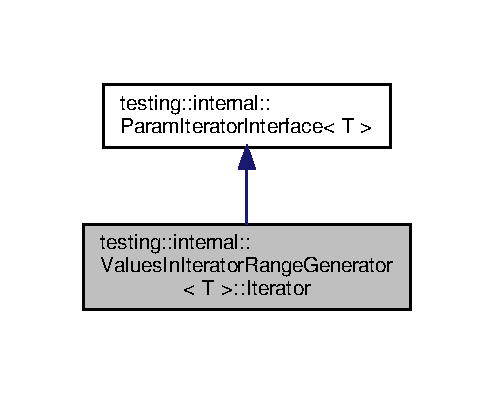
\includegraphics[width=237pt]{classtesting_1_1internal_1_1ValuesInIteratorRangeGenerator_1_1Iterator__inherit__graph}
\end{center}
\end{figure}


Collaboration diagram for testing\+:\+:internal\+:\+:Values\+In\+Iterator\+Range\+Generator$<$ T $>$\+:\+:Iterator\+:\nopagebreak
\begin{figure}[H]
\begin{center}
\leavevmode
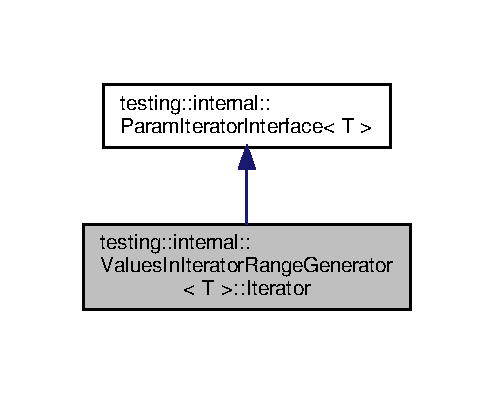
\includegraphics[width=237pt]{classtesting_1_1internal_1_1ValuesInIteratorRangeGenerator_1_1Iterator__coll__graph}
\end{center}
\end{figure}
\subsection*{Public Member Functions}
\begin{DoxyCompactItemize}
\item 
\hyperlink{classtesting_1_1internal_1_1ValuesInIteratorRangeGenerator_1_1Iterator_aebd635efe7082e6fc45bb8ae0dbefd2e}{Iterator} (const \hyperlink{classtesting_1_1internal_1_1ParamGeneratorInterface}{Param\+Generator\+Interface}$<$ T $>$ $\ast$base, typename Container\+Type\+::const\+\_\+iterator iterator)
\item 
\hyperlink{classtesting_1_1internal_1_1ValuesInIteratorRangeGenerator_1_1Iterator_a265c1facb4cbd4669686d5f331df4a95}{$\sim$\+Iterator} () override
\item 
const \hyperlink{classtesting_1_1internal_1_1ParamGeneratorInterface}{Param\+Generator\+Interface}$<$ T $>$ $\ast$ \hyperlink{classtesting_1_1internal_1_1ValuesInIteratorRangeGenerator_1_1Iterator_a27445e4d010ffde9d3f2f9ada5d54d0f}{Base\+Generator} () const override
\item 
void \hyperlink{classtesting_1_1internal_1_1ValuesInIteratorRangeGenerator_1_1Iterator_a5ff56489536cf5d90ed0ac07ffeb476b}{Advance} () override
\item 
\hyperlink{classtesting_1_1internal_1_1ParamIteratorInterface}{Param\+Iterator\+Interface}$<$ T $>$ $\ast$ \hyperlink{classtesting_1_1internal_1_1ValuesInIteratorRangeGenerator_1_1Iterator_a2c5ccf4da12cfb089829438d679ae35e}{Clone} () const override
\item 
const T $\ast$ \hyperlink{classtesting_1_1internal_1_1ValuesInIteratorRangeGenerator_1_1Iterator_a55bd2a0d5a630478e32ec2efe08e37e4}{Current} () const override
\item 
bool \hyperlink{classtesting_1_1internal_1_1ValuesInIteratorRangeGenerator_1_1Iterator_a75604bc318aca22ff8607b68bfb44e96}{Equals} (const \hyperlink{classtesting_1_1internal_1_1ParamIteratorInterface}{Param\+Iterator\+Interface}$<$ T $>$ \&other) const override
\end{DoxyCompactItemize}
\subsection*{Private Member Functions}
\begin{DoxyCompactItemize}
\item 
\hyperlink{classtesting_1_1internal_1_1ValuesInIteratorRangeGenerator_1_1Iterator_a87cadeed020bb8bfbdce636fca31b9ef}{Iterator} (const \hyperlink{classtesting_1_1internal_1_1ValuesInIteratorRangeGenerator_1_1Iterator}{Iterator} \&other)
\end{DoxyCompactItemize}
\subsection*{Private Attributes}
\begin{DoxyCompactItemize}
\item 
const \hyperlink{classtesting_1_1internal_1_1ParamGeneratorInterface}{Param\+Generator\+Interface}$<$ T $>$ $\ast$const \hyperlink{classtesting_1_1internal_1_1ValuesInIteratorRangeGenerator_1_1Iterator_a904df7e46beda1ce5ac2c0ecd6680e0d}{base\+\_\+}
\item 
Container\+Type\+::const\+\_\+iterator \hyperlink{classtesting_1_1internal_1_1ValuesInIteratorRangeGenerator_1_1Iterator_aaff15b9f8addac71b91c32053bf9ea1e}{iterator\+\_\+}
\item 
std\+::unique\+\_\+ptr$<$ const T $>$ \hyperlink{classtesting_1_1internal_1_1ValuesInIteratorRangeGenerator_1_1Iterator_af51f1a21ffb0cd531de7574f4ad1f9b6}{value\+\_\+}
\end{DoxyCompactItemize}


\subsection{Constructor \& Destructor Documentation}
\mbox{\Hypertarget{classtesting_1_1internal_1_1ValuesInIteratorRangeGenerator_1_1Iterator_aebd635efe7082e6fc45bb8ae0dbefd2e}\label{classtesting_1_1internal_1_1ValuesInIteratorRangeGenerator_1_1Iterator_aebd635efe7082e6fc45bb8ae0dbefd2e}} 
\index{testing\+::internal\+::\+Values\+In\+Iterator\+Range\+Generator\+::\+Iterator@{testing\+::internal\+::\+Values\+In\+Iterator\+Range\+Generator\+::\+Iterator}!Iterator@{Iterator}}
\index{Iterator@{Iterator}!testing\+::internal\+::\+Values\+In\+Iterator\+Range\+Generator\+::\+Iterator@{testing\+::internal\+::\+Values\+In\+Iterator\+Range\+Generator\+::\+Iterator}}
\subsubsection{\texorpdfstring{Iterator()}{Iterator()}\hspace{0.1cm}{\footnotesize\ttfamily [1/2]}}
{\footnotesize\ttfamily template$<$typename T $>$ \\
\hyperlink{classtesting_1_1internal_1_1ValuesInIteratorRangeGenerator}{testing\+::internal\+::\+Values\+In\+Iterator\+Range\+Generator}$<$ T $>$\+::Iterator\+::\+Iterator (\begin{DoxyParamCaption}\item[{const \hyperlink{classtesting_1_1internal_1_1ParamGeneratorInterface}{Param\+Generator\+Interface}$<$ T $>$ $\ast$}]{base,  }\item[{typename Container\+Type\+::const\+\_\+iterator}]{iterator }\end{DoxyParamCaption})\hspace{0.3cm}{\ttfamily [inline]}}

\mbox{\Hypertarget{classtesting_1_1internal_1_1ValuesInIteratorRangeGenerator_1_1Iterator_a265c1facb4cbd4669686d5f331df4a95}\label{classtesting_1_1internal_1_1ValuesInIteratorRangeGenerator_1_1Iterator_a265c1facb4cbd4669686d5f331df4a95}} 
\index{testing\+::internal\+::\+Values\+In\+Iterator\+Range\+Generator\+::\+Iterator@{testing\+::internal\+::\+Values\+In\+Iterator\+Range\+Generator\+::\+Iterator}!````~Iterator@{$\sim$\+Iterator}}
\index{````~Iterator@{$\sim$\+Iterator}!testing\+::internal\+::\+Values\+In\+Iterator\+Range\+Generator\+::\+Iterator@{testing\+::internal\+::\+Values\+In\+Iterator\+Range\+Generator\+::\+Iterator}}
\subsubsection{\texorpdfstring{$\sim$\+Iterator()}{~Iterator()}}
{\footnotesize\ttfamily template$<$typename T $>$ \\
\hyperlink{classtesting_1_1internal_1_1ValuesInIteratorRangeGenerator}{testing\+::internal\+::\+Values\+In\+Iterator\+Range\+Generator}$<$ T $>$\+::Iterator\+::$\sim$\+Iterator (\begin{DoxyParamCaption}{ }\end{DoxyParamCaption})\hspace{0.3cm}{\ttfamily [inline]}, {\ttfamily [override]}}

\mbox{\Hypertarget{classtesting_1_1internal_1_1ValuesInIteratorRangeGenerator_1_1Iterator_a87cadeed020bb8bfbdce636fca31b9ef}\label{classtesting_1_1internal_1_1ValuesInIteratorRangeGenerator_1_1Iterator_a87cadeed020bb8bfbdce636fca31b9ef}} 
\index{testing\+::internal\+::\+Values\+In\+Iterator\+Range\+Generator\+::\+Iterator@{testing\+::internal\+::\+Values\+In\+Iterator\+Range\+Generator\+::\+Iterator}!Iterator@{Iterator}}
\index{Iterator@{Iterator}!testing\+::internal\+::\+Values\+In\+Iterator\+Range\+Generator\+::\+Iterator@{testing\+::internal\+::\+Values\+In\+Iterator\+Range\+Generator\+::\+Iterator}}
\subsubsection{\texorpdfstring{Iterator()}{Iterator()}\hspace{0.1cm}{\footnotesize\ttfamily [2/2]}}
{\footnotesize\ttfamily template$<$typename T $>$ \\
\hyperlink{classtesting_1_1internal_1_1ValuesInIteratorRangeGenerator}{testing\+::internal\+::\+Values\+In\+Iterator\+Range\+Generator}$<$ T $>$\+::Iterator\+::\+Iterator (\begin{DoxyParamCaption}\item[{const \hyperlink{classtesting_1_1internal_1_1ValuesInIteratorRangeGenerator_1_1Iterator}{Iterator} \&}]{other }\end{DoxyParamCaption})\hspace{0.3cm}{\ttfamily [inline]}, {\ttfamily [private]}}



\subsection{Member Function Documentation}
\mbox{\Hypertarget{classtesting_1_1internal_1_1ValuesInIteratorRangeGenerator_1_1Iterator_a5ff56489536cf5d90ed0ac07ffeb476b}\label{classtesting_1_1internal_1_1ValuesInIteratorRangeGenerator_1_1Iterator_a5ff56489536cf5d90ed0ac07ffeb476b}} 
\index{testing\+::internal\+::\+Values\+In\+Iterator\+Range\+Generator\+::\+Iterator@{testing\+::internal\+::\+Values\+In\+Iterator\+Range\+Generator\+::\+Iterator}!Advance@{Advance}}
\index{Advance@{Advance}!testing\+::internal\+::\+Values\+In\+Iterator\+Range\+Generator\+::\+Iterator@{testing\+::internal\+::\+Values\+In\+Iterator\+Range\+Generator\+::\+Iterator}}
\subsubsection{\texorpdfstring{Advance()}{Advance()}}
{\footnotesize\ttfamily template$<$typename T $>$ \\
void \hyperlink{classtesting_1_1internal_1_1ValuesInIteratorRangeGenerator}{testing\+::internal\+::\+Values\+In\+Iterator\+Range\+Generator}$<$ T $>$\+::Iterator\+::\+Advance (\begin{DoxyParamCaption}{ }\end{DoxyParamCaption})\hspace{0.3cm}{\ttfamily [inline]}, {\ttfamily [override]}, {\ttfamily [virtual]}}



Implements \hyperlink{classtesting_1_1internal_1_1ParamIteratorInterface_a600dbd35fcb551463e379516a1abea48}{testing\+::internal\+::\+Param\+Iterator\+Interface$<$ T $>$}.

\mbox{\Hypertarget{classtesting_1_1internal_1_1ValuesInIteratorRangeGenerator_1_1Iterator_a27445e4d010ffde9d3f2f9ada5d54d0f}\label{classtesting_1_1internal_1_1ValuesInIteratorRangeGenerator_1_1Iterator_a27445e4d010ffde9d3f2f9ada5d54d0f}} 
\index{testing\+::internal\+::\+Values\+In\+Iterator\+Range\+Generator\+::\+Iterator@{testing\+::internal\+::\+Values\+In\+Iterator\+Range\+Generator\+::\+Iterator}!Base\+Generator@{Base\+Generator}}
\index{Base\+Generator@{Base\+Generator}!testing\+::internal\+::\+Values\+In\+Iterator\+Range\+Generator\+::\+Iterator@{testing\+::internal\+::\+Values\+In\+Iterator\+Range\+Generator\+::\+Iterator}}
\subsubsection{\texorpdfstring{Base\+Generator()}{BaseGenerator()}}
{\footnotesize\ttfamily template$<$typename T $>$ \\
const \hyperlink{classtesting_1_1internal_1_1ParamGeneratorInterface}{Param\+Generator\+Interface}$<$T$>$$\ast$ \hyperlink{classtesting_1_1internal_1_1ValuesInIteratorRangeGenerator}{testing\+::internal\+::\+Values\+In\+Iterator\+Range\+Generator}$<$ T $>$\+::Iterator\+::\+Base\+Generator (\begin{DoxyParamCaption}{ }\end{DoxyParamCaption}) const\hspace{0.3cm}{\ttfamily [inline]}, {\ttfamily [override]}, {\ttfamily [virtual]}}



Implements \hyperlink{classtesting_1_1internal_1_1ParamIteratorInterface_a17500953df75ecda1ace46c08ff731e9}{testing\+::internal\+::\+Param\+Iterator\+Interface$<$ T $>$}.

\mbox{\Hypertarget{classtesting_1_1internal_1_1ValuesInIteratorRangeGenerator_1_1Iterator_a2c5ccf4da12cfb089829438d679ae35e}\label{classtesting_1_1internal_1_1ValuesInIteratorRangeGenerator_1_1Iterator_a2c5ccf4da12cfb089829438d679ae35e}} 
\index{testing\+::internal\+::\+Values\+In\+Iterator\+Range\+Generator\+::\+Iterator@{testing\+::internal\+::\+Values\+In\+Iterator\+Range\+Generator\+::\+Iterator}!Clone@{Clone}}
\index{Clone@{Clone}!testing\+::internal\+::\+Values\+In\+Iterator\+Range\+Generator\+::\+Iterator@{testing\+::internal\+::\+Values\+In\+Iterator\+Range\+Generator\+::\+Iterator}}
\subsubsection{\texorpdfstring{Clone()}{Clone()}}
{\footnotesize\ttfamily template$<$typename T $>$ \\
\hyperlink{classtesting_1_1internal_1_1ParamIteratorInterface}{Param\+Iterator\+Interface}$<$T$>$$\ast$ \hyperlink{classtesting_1_1internal_1_1ValuesInIteratorRangeGenerator}{testing\+::internal\+::\+Values\+In\+Iterator\+Range\+Generator}$<$ T $>$\+::Iterator\+::\+Clone (\begin{DoxyParamCaption}{ }\end{DoxyParamCaption}) const\hspace{0.3cm}{\ttfamily [inline]}, {\ttfamily [override]}, {\ttfamily [virtual]}}



Implements \hyperlink{classtesting_1_1internal_1_1ParamIteratorInterface_a4998c23e27e2943d97546011aa35db80}{testing\+::internal\+::\+Param\+Iterator\+Interface$<$ T $>$}.

\mbox{\Hypertarget{classtesting_1_1internal_1_1ValuesInIteratorRangeGenerator_1_1Iterator_a55bd2a0d5a630478e32ec2efe08e37e4}\label{classtesting_1_1internal_1_1ValuesInIteratorRangeGenerator_1_1Iterator_a55bd2a0d5a630478e32ec2efe08e37e4}} 
\index{testing\+::internal\+::\+Values\+In\+Iterator\+Range\+Generator\+::\+Iterator@{testing\+::internal\+::\+Values\+In\+Iterator\+Range\+Generator\+::\+Iterator}!Current@{Current}}
\index{Current@{Current}!testing\+::internal\+::\+Values\+In\+Iterator\+Range\+Generator\+::\+Iterator@{testing\+::internal\+::\+Values\+In\+Iterator\+Range\+Generator\+::\+Iterator}}
\subsubsection{\texorpdfstring{Current()}{Current()}}
{\footnotesize\ttfamily template$<$typename T $>$ \\
const T$\ast$ \hyperlink{classtesting_1_1internal_1_1ValuesInIteratorRangeGenerator}{testing\+::internal\+::\+Values\+In\+Iterator\+Range\+Generator}$<$ T $>$\+::Iterator\+::\+Current (\begin{DoxyParamCaption}{ }\end{DoxyParamCaption}) const\hspace{0.3cm}{\ttfamily [inline]}, {\ttfamily [override]}, {\ttfamily [virtual]}}



Implements \hyperlink{classtesting_1_1internal_1_1ParamIteratorInterface_adfff808576d929085679c315b255af7e}{testing\+::internal\+::\+Param\+Iterator\+Interface$<$ T $>$}.

\mbox{\Hypertarget{classtesting_1_1internal_1_1ValuesInIteratorRangeGenerator_1_1Iterator_a75604bc318aca22ff8607b68bfb44e96}\label{classtesting_1_1internal_1_1ValuesInIteratorRangeGenerator_1_1Iterator_a75604bc318aca22ff8607b68bfb44e96}} 
\index{testing\+::internal\+::\+Values\+In\+Iterator\+Range\+Generator\+::\+Iterator@{testing\+::internal\+::\+Values\+In\+Iterator\+Range\+Generator\+::\+Iterator}!Equals@{Equals}}
\index{Equals@{Equals}!testing\+::internal\+::\+Values\+In\+Iterator\+Range\+Generator\+::\+Iterator@{testing\+::internal\+::\+Values\+In\+Iterator\+Range\+Generator\+::\+Iterator}}
\subsubsection{\texorpdfstring{Equals()}{Equals()}}
{\footnotesize\ttfamily template$<$typename T $>$ \\
bool \hyperlink{classtesting_1_1internal_1_1ValuesInIteratorRangeGenerator}{testing\+::internal\+::\+Values\+In\+Iterator\+Range\+Generator}$<$ T $>$\+::Iterator\+::\+Equals (\begin{DoxyParamCaption}\item[{const \hyperlink{classtesting_1_1internal_1_1ParamIteratorInterface}{Param\+Iterator\+Interface}$<$ T $>$ \&}]{other }\end{DoxyParamCaption}) const\hspace{0.3cm}{\ttfamily [inline]}, {\ttfamily [override]}, {\ttfamily [virtual]}}



Implements \hyperlink{classtesting_1_1internal_1_1ParamIteratorInterface_a9d811697a752d46f7bd6a0082f9040a3}{testing\+::internal\+::\+Param\+Iterator\+Interface$<$ T $>$}.



\subsection{Member Data Documentation}
\mbox{\Hypertarget{classtesting_1_1internal_1_1ValuesInIteratorRangeGenerator_1_1Iterator_a904df7e46beda1ce5ac2c0ecd6680e0d}\label{classtesting_1_1internal_1_1ValuesInIteratorRangeGenerator_1_1Iterator_a904df7e46beda1ce5ac2c0ecd6680e0d}} 
\index{testing\+::internal\+::\+Values\+In\+Iterator\+Range\+Generator\+::\+Iterator@{testing\+::internal\+::\+Values\+In\+Iterator\+Range\+Generator\+::\+Iterator}!base\+\_\+@{base\+\_\+}}
\index{base\+\_\+@{base\+\_\+}!testing\+::internal\+::\+Values\+In\+Iterator\+Range\+Generator\+::\+Iterator@{testing\+::internal\+::\+Values\+In\+Iterator\+Range\+Generator\+::\+Iterator}}
\subsubsection{\texorpdfstring{base\+\_\+}{base\_}}
{\footnotesize\ttfamily template$<$typename T $>$ \\
const \hyperlink{classtesting_1_1internal_1_1ParamGeneratorInterface}{Param\+Generator\+Interface}$<$T$>$$\ast$ const \hyperlink{classtesting_1_1internal_1_1ValuesInIteratorRangeGenerator}{testing\+::internal\+::\+Values\+In\+Iterator\+Range\+Generator}$<$ T $>$\+::Iterator\+::base\+\_\+\hspace{0.3cm}{\ttfamily [private]}}

\mbox{\Hypertarget{classtesting_1_1internal_1_1ValuesInIteratorRangeGenerator_1_1Iterator_aaff15b9f8addac71b91c32053bf9ea1e}\label{classtesting_1_1internal_1_1ValuesInIteratorRangeGenerator_1_1Iterator_aaff15b9f8addac71b91c32053bf9ea1e}} 
\index{testing\+::internal\+::\+Values\+In\+Iterator\+Range\+Generator\+::\+Iterator@{testing\+::internal\+::\+Values\+In\+Iterator\+Range\+Generator\+::\+Iterator}!iterator\+\_\+@{iterator\+\_\+}}
\index{iterator\+\_\+@{iterator\+\_\+}!testing\+::internal\+::\+Values\+In\+Iterator\+Range\+Generator\+::\+Iterator@{testing\+::internal\+::\+Values\+In\+Iterator\+Range\+Generator\+::\+Iterator}}
\subsubsection{\texorpdfstring{iterator\+\_\+}{iterator\_}}
{\footnotesize\ttfamily template$<$typename T $>$ \\
Container\+Type\+::const\+\_\+iterator \hyperlink{classtesting_1_1internal_1_1ValuesInIteratorRangeGenerator}{testing\+::internal\+::\+Values\+In\+Iterator\+Range\+Generator}$<$ T $>$\+::Iterator\+::iterator\+\_\+\hspace{0.3cm}{\ttfamily [private]}}

\mbox{\Hypertarget{classtesting_1_1internal_1_1ValuesInIteratorRangeGenerator_1_1Iterator_af51f1a21ffb0cd531de7574f4ad1f9b6}\label{classtesting_1_1internal_1_1ValuesInIteratorRangeGenerator_1_1Iterator_af51f1a21ffb0cd531de7574f4ad1f9b6}} 
\index{testing\+::internal\+::\+Values\+In\+Iterator\+Range\+Generator\+::\+Iterator@{testing\+::internal\+::\+Values\+In\+Iterator\+Range\+Generator\+::\+Iterator}!value\+\_\+@{value\+\_\+}}
\index{value\+\_\+@{value\+\_\+}!testing\+::internal\+::\+Values\+In\+Iterator\+Range\+Generator\+::\+Iterator@{testing\+::internal\+::\+Values\+In\+Iterator\+Range\+Generator\+::\+Iterator}}
\subsubsection{\texorpdfstring{value\+\_\+}{value\_}}
{\footnotesize\ttfamily template$<$typename T $>$ \\
std\+::unique\+\_\+ptr$<$const T$>$ \hyperlink{classtesting_1_1internal_1_1ValuesInIteratorRangeGenerator}{testing\+::internal\+::\+Values\+In\+Iterator\+Range\+Generator}$<$ T $>$\+::Iterator\+::value\+\_\+\hspace{0.3cm}{\ttfamily [mutable]}, {\ttfamily [private]}}



The documentation for this class was generated from the following file\+:\begin{DoxyCompactItemize}
\item 
tests/googletest/include/gtest/internal/\hyperlink{gtest-param-util_8h}{gtest-\/param-\/util.\+h}\end{DoxyCompactItemize}

\hypertarget{classtesting_1_1internal_1_1CartesianProductGenerator_1_1IteratorImpl}{}\section{testing\+:\+:internal\+:\+:Cartesian\+Product\+Generator$<$ T $>$\+:\+:Iterator\+Impl$<$ I $>$ Class Template Reference}
\label{classtesting_1_1internal_1_1CartesianProductGenerator_1_1IteratorImpl}\index{testing\+::internal\+::\+Cartesian\+Product\+Generator$<$ T $>$\+::\+Iterator\+Impl$<$ I $>$@{testing\+::internal\+::\+Cartesian\+Product\+Generator$<$ T $>$\+::\+Iterator\+Impl$<$ I $>$}}


The documentation for this class was generated from the following file\+:\begin{DoxyCompactItemize}
\item 
tests/googletest/include/gtest/internal/\hyperlink{gtest-param-util_8h}{gtest-\/param-\/util.\+h}\end{DoxyCompactItemize}

\hypertarget{classtesting_1_1internal_1_1CartesianProductGenerator_1_1IteratorImpl_3_01IndexSequence_3_01I_8_8_8_01_4_01_4}{}\section{testing\+:\+:internal\+:\+:Cartesian\+Product\+Generator$<$ T $>$\+:\+:Iterator\+Impl$<$ Index\+Sequence$<$ I... $>$ $>$ Class Template Reference}
\label{classtesting_1_1internal_1_1CartesianProductGenerator_1_1IteratorImpl_3_01IndexSequence_3_01I_8_8_8_01_4_01_4}\index{testing\+::internal\+::\+Cartesian\+Product\+Generator$<$ T $>$\+::\+Iterator\+Impl$<$ Index\+Sequence$<$ I... $>$ $>$@{testing\+::internal\+::\+Cartesian\+Product\+Generator$<$ T $>$\+::\+Iterator\+Impl$<$ Index\+Sequence$<$ I... $>$ $>$}}


Inheritance diagram for testing\+:\+:internal\+:\+:Cartesian\+Product\+Generator$<$ T $>$\+:\+:Iterator\+Impl$<$ Index\+Sequence$<$ I... $>$ $>$\+:\nopagebreak
\begin{figure}[H]
\begin{center}
\leavevmode
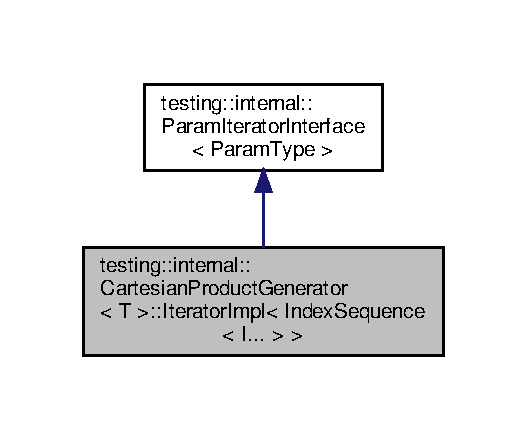
\includegraphics[width=253pt]{classtesting_1_1internal_1_1CartesianProductGenerator_1_1IteratorImpl_3_01IndexSequence_3_01I_8_8_8_01_4_01_4__inherit__graph}
\end{center}
\end{figure}


Collaboration diagram for testing\+:\+:internal\+:\+:Cartesian\+Product\+Generator$<$ T $>$\+:\+:Iterator\+Impl$<$ Index\+Sequence$<$ I... $>$ $>$\+:\nopagebreak
\begin{figure}[H]
\begin{center}
\leavevmode
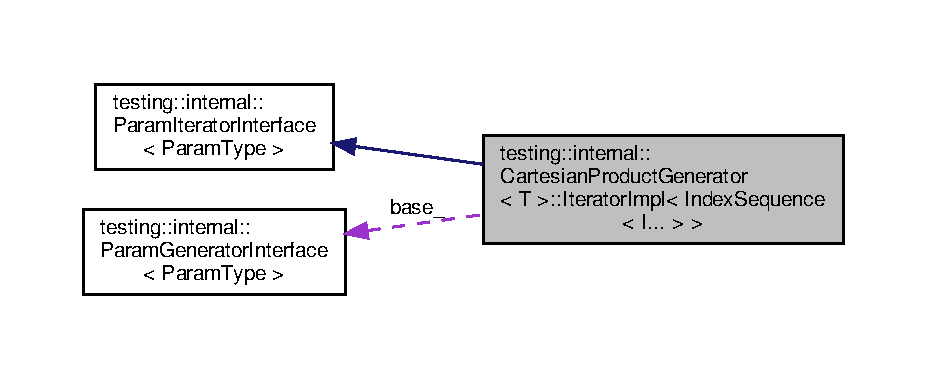
\includegraphics[width=350pt]{classtesting_1_1internal_1_1CartesianProductGenerator_1_1IteratorImpl_3_01IndexSequence_3_01I_8_8_8_01_4_01_4__coll__graph}
\end{center}
\end{figure}
\subsection*{Public Member Functions}
\begin{DoxyCompactItemize}
\item 
\hyperlink{classtesting_1_1internal_1_1CartesianProductGenerator_1_1IteratorImpl_3_01IndexSequence_3_01I_8_8_8_01_4_01_4_a3c28d20b4527f146a97c5490326f869f}{Iterator\+Impl} (const \hyperlink{classtesting_1_1internal_1_1ParamGeneratorInterface}{Param\+Generator\+Interface}$<$ \hyperlink{classtesting_1_1internal_1_1CartesianProductGenerator_af27131157a9347f0c82420ca081ee7dd}{Param\+Type} $>$ $\ast$base, const std\+::tuple$<$ \hyperlink{classtesting_1_1internal_1_1ParamGenerator}{Param\+Generator}$<$ T $>$... $>$ \&generators, bool is\+\_\+end)
\item 
\hyperlink{classtesting_1_1internal_1_1CartesianProductGenerator_1_1IteratorImpl_3_01IndexSequence_3_01I_8_8_8_01_4_01_4_adf6a47392283d7e236b604f487cf8cfc}{$\sim$\+Iterator\+Impl} () override
\item 
const \hyperlink{classtesting_1_1internal_1_1ParamGeneratorInterface}{Param\+Generator\+Interface}$<$ \hyperlink{classtesting_1_1internal_1_1CartesianProductGenerator_af27131157a9347f0c82420ca081ee7dd}{Param\+Type} $>$ $\ast$ \hyperlink{classtesting_1_1internal_1_1CartesianProductGenerator_1_1IteratorImpl_3_01IndexSequence_3_01I_8_8_8_01_4_01_4_a8fa3ea322a1348fc8065481aba76e860}{Base\+Generator} () const override
\item 
void \hyperlink{classtesting_1_1internal_1_1CartesianProductGenerator_1_1IteratorImpl_3_01IndexSequence_3_01I_8_8_8_01_4_01_4_a167e8b38118c8635d5849daf924a517b}{Advance} () override
\item 
\hyperlink{classtesting_1_1internal_1_1ParamIteratorInterface}{Param\+Iterator\+Interface}$<$ \hyperlink{classtesting_1_1internal_1_1CartesianProductGenerator_af27131157a9347f0c82420ca081ee7dd}{Param\+Type} $>$ $\ast$ \hyperlink{classtesting_1_1internal_1_1CartesianProductGenerator_1_1IteratorImpl_3_01IndexSequence_3_01I_8_8_8_01_4_01_4_a0b434e09b32dfd6b444085cf95dc22ab}{Clone} () const override
\item 
const \hyperlink{classtesting_1_1internal_1_1CartesianProductGenerator_af27131157a9347f0c82420ca081ee7dd}{Param\+Type} $\ast$ \hyperlink{classtesting_1_1internal_1_1CartesianProductGenerator_1_1IteratorImpl_3_01IndexSequence_3_01I_8_8_8_01_4_01_4_ab7052f320ab8ff3113a3e744a1bff07e}{Current} () const override
\item 
bool \hyperlink{classtesting_1_1internal_1_1CartesianProductGenerator_1_1IteratorImpl_3_01IndexSequence_3_01I_8_8_8_01_4_01_4_a7ba6129ccd025c1cb0e00fe71b8c8489}{Equals} (const \hyperlink{classtesting_1_1internal_1_1ParamIteratorInterface}{Param\+Iterator\+Interface}$<$ \hyperlink{classtesting_1_1internal_1_1CartesianProductGenerator_af27131157a9347f0c82420ca081ee7dd}{Param\+Type} $>$ \&other) const override
\end{DoxyCompactItemize}
\subsection*{Private Member Functions}
\begin{DoxyCompactItemize}
\item 
{\footnotesize template$<$size\+\_\+t ThisI$>$ }\\void \hyperlink{classtesting_1_1internal_1_1CartesianProductGenerator_1_1IteratorImpl_3_01IndexSequence_3_01I_8_8_8_01_4_01_4_a6a5fd8b4a0cd8e27c0ca1fbbfee4f997}{Advance\+If\+End} ()
\item 
void \hyperlink{classtesting_1_1internal_1_1CartesianProductGenerator_1_1IteratorImpl_3_01IndexSequence_3_01I_8_8_8_01_4_01_4_a0e6c088fed9a27254a657755d05bdcae}{Compute\+Current\+Value} ()
\item 
bool \hyperlink{classtesting_1_1internal_1_1CartesianProductGenerator_1_1IteratorImpl_3_01IndexSequence_3_01I_8_8_8_01_4_01_4_abdf53ad1a435b992d399210178b35b70}{At\+End} () const
\end{DoxyCompactItemize}
\subsection*{Private Attributes}
\begin{DoxyCompactItemize}
\item 
const \hyperlink{classtesting_1_1internal_1_1ParamGeneratorInterface}{Param\+Generator\+Interface}$<$ \hyperlink{classtesting_1_1internal_1_1CartesianProductGenerator_af27131157a9347f0c82420ca081ee7dd}{Param\+Type} $>$ $\ast$const \hyperlink{classtesting_1_1internal_1_1CartesianProductGenerator_1_1IteratorImpl_3_01IndexSequence_3_01I_8_8_8_01_4_01_4_ae434c3fd6b3fc5055960563a6d550376}{base\+\_\+}
\item 
std\+::tuple$<$ typename \hyperlink{classtesting_1_1internal_1_1ParamGenerator}{Param\+Generator}$<$ T $>$\+::iterator... $>$ \hyperlink{classtesting_1_1internal_1_1CartesianProductGenerator_1_1IteratorImpl_3_01IndexSequence_3_01I_8_8_8_01_4_01_4_aae7fbddbf01df185226712ee2a38d410}{begin\+\_\+}
\item 
std\+::tuple$<$ typename \hyperlink{classtesting_1_1internal_1_1ParamGenerator}{Param\+Generator}$<$ T $>$\+::iterator... $>$ \hyperlink{classtesting_1_1internal_1_1CartesianProductGenerator_1_1IteratorImpl_3_01IndexSequence_3_01I_8_8_8_01_4_01_4_aae9ccfd177834224412f9ac194bd8b68}{end\+\_\+}
\item 
std\+::tuple$<$ typename \hyperlink{classtesting_1_1internal_1_1ParamGenerator}{Param\+Generator}$<$ T $>$\+::iterator... $>$ \hyperlink{classtesting_1_1internal_1_1CartesianProductGenerator_1_1IteratorImpl_3_01IndexSequence_3_01I_8_8_8_01_4_01_4_a0678508a97f8b218fb5af11915678abf}{current\+\_\+}
\item 
std\+::shared\+\_\+ptr$<$ \hyperlink{classtesting_1_1internal_1_1CartesianProductGenerator_af27131157a9347f0c82420ca081ee7dd}{Param\+Type} $>$ \hyperlink{classtesting_1_1internal_1_1CartesianProductGenerator_1_1IteratorImpl_3_01IndexSequence_3_01I_8_8_8_01_4_01_4_ab7ce5ae5ae5dbdcca97e1824d77736b0}{current\+\_\+value\+\_\+}
\end{DoxyCompactItemize}


\subsection{Constructor \& Destructor Documentation}
\mbox{\Hypertarget{classtesting_1_1internal_1_1CartesianProductGenerator_1_1IteratorImpl_3_01IndexSequence_3_01I_8_8_8_01_4_01_4_a3c28d20b4527f146a97c5490326f869f}\label{classtesting_1_1internal_1_1CartesianProductGenerator_1_1IteratorImpl_3_01IndexSequence_3_01I_8_8_8_01_4_01_4_a3c28d20b4527f146a97c5490326f869f}} 
\index{testing\+::internal\+::\+Cartesian\+Product\+Generator\+::\+Iterator\+Impl$<$ Index\+Sequence$<$ I... $>$ $>$@{testing\+::internal\+::\+Cartesian\+Product\+Generator\+::\+Iterator\+Impl$<$ Index\+Sequence$<$ I... $>$ $>$}!Iterator\+Impl@{Iterator\+Impl}}
\index{Iterator\+Impl@{Iterator\+Impl}!testing\+::internal\+::\+Cartesian\+Product\+Generator\+::\+Iterator\+Impl$<$ Index\+Sequence$<$ I... $>$ $>$@{testing\+::internal\+::\+Cartesian\+Product\+Generator\+::\+Iterator\+Impl$<$ Index\+Sequence$<$ I... $>$ $>$}}
\subsubsection{\texorpdfstring{Iterator\+Impl()}{IteratorImpl()}}
{\footnotesize\ttfamily template$<$typename... T$>$ \\
template$<$size\+\_\+t... I$>$ \\
\hyperlink{classtesting_1_1internal_1_1CartesianProductGenerator}{testing\+::internal\+::\+Cartesian\+Product\+Generator}$<$ T $>$\+::\hyperlink{classtesting_1_1internal_1_1CartesianProductGenerator_1_1IteratorImpl}{Iterator\+Impl}$<$ \hyperlink{structtesting_1_1internal_1_1IndexSequence}{Index\+Sequence}$<$ I... $>$ $>$\+::\hyperlink{classtesting_1_1internal_1_1CartesianProductGenerator_1_1IteratorImpl}{Iterator\+Impl} (\begin{DoxyParamCaption}\item[{const \hyperlink{classtesting_1_1internal_1_1ParamGeneratorInterface}{Param\+Generator\+Interface}$<$ \hyperlink{classtesting_1_1internal_1_1CartesianProductGenerator_af27131157a9347f0c82420ca081ee7dd}{Param\+Type} $>$ $\ast$}]{base,  }\item[{const std\+::tuple$<$ \hyperlink{classtesting_1_1internal_1_1ParamGenerator}{Param\+Generator}$<$ T $>$... $>$ \&}]{generators,  }\item[{bool}]{is\+\_\+end }\end{DoxyParamCaption})\hspace{0.3cm}{\ttfamily [inline]}}

\mbox{\Hypertarget{classtesting_1_1internal_1_1CartesianProductGenerator_1_1IteratorImpl_3_01IndexSequence_3_01I_8_8_8_01_4_01_4_adf6a47392283d7e236b604f487cf8cfc}\label{classtesting_1_1internal_1_1CartesianProductGenerator_1_1IteratorImpl_3_01IndexSequence_3_01I_8_8_8_01_4_01_4_adf6a47392283d7e236b604f487cf8cfc}} 
\index{testing\+::internal\+::\+Cartesian\+Product\+Generator\+::\+Iterator\+Impl$<$ Index\+Sequence$<$ I... $>$ $>$@{testing\+::internal\+::\+Cartesian\+Product\+Generator\+::\+Iterator\+Impl$<$ Index\+Sequence$<$ I... $>$ $>$}!````~Iterator\+Impl@{$\sim$\+Iterator\+Impl}}
\index{````~Iterator\+Impl@{$\sim$\+Iterator\+Impl}!testing\+::internal\+::\+Cartesian\+Product\+Generator\+::\+Iterator\+Impl$<$ Index\+Sequence$<$ I... $>$ $>$@{testing\+::internal\+::\+Cartesian\+Product\+Generator\+::\+Iterator\+Impl$<$ Index\+Sequence$<$ I... $>$ $>$}}
\subsubsection{\texorpdfstring{$\sim$\+Iterator\+Impl()}{~IteratorImpl()}}
{\footnotesize\ttfamily template$<$typename... T$>$ \\
template$<$size\+\_\+t... I$>$ \\
\hyperlink{classtesting_1_1internal_1_1CartesianProductGenerator}{testing\+::internal\+::\+Cartesian\+Product\+Generator}$<$ T $>$\+::\hyperlink{classtesting_1_1internal_1_1CartesianProductGenerator_1_1IteratorImpl}{Iterator\+Impl}$<$ \hyperlink{structtesting_1_1internal_1_1IndexSequence}{Index\+Sequence}$<$ I... $>$ $>$\+::$\sim$\hyperlink{classtesting_1_1internal_1_1CartesianProductGenerator_1_1IteratorImpl}{Iterator\+Impl} (\begin{DoxyParamCaption}{ }\end{DoxyParamCaption})\hspace{0.3cm}{\ttfamily [inline]}, {\ttfamily [override]}}



\subsection{Member Function Documentation}
\mbox{\Hypertarget{classtesting_1_1internal_1_1CartesianProductGenerator_1_1IteratorImpl_3_01IndexSequence_3_01I_8_8_8_01_4_01_4_a167e8b38118c8635d5849daf924a517b}\label{classtesting_1_1internal_1_1CartesianProductGenerator_1_1IteratorImpl_3_01IndexSequence_3_01I_8_8_8_01_4_01_4_a167e8b38118c8635d5849daf924a517b}} 
\index{testing\+::internal\+::\+Cartesian\+Product\+Generator\+::\+Iterator\+Impl$<$ Index\+Sequence$<$ I... $>$ $>$@{testing\+::internal\+::\+Cartesian\+Product\+Generator\+::\+Iterator\+Impl$<$ Index\+Sequence$<$ I... $>$ $>$}!Advance@{Advance}}
\index{Advance@{Advance}!testing\+::internal\+::\+Cartesian\+Product\+Generator\+::\+Iterator\+Impl$<$ Index\+Sequence$<$ I... $>$ $>$@{testing\+::internal\+::\+Cartesian\+Product\+Generator\+::\+Iterator\+Impl$<$ Index\+Sequence$<$ I... $>$ $>$}}
\subsubsection{\texorpdfstring{Advance()}{Advance()}}
{\footnotesize\ttfamily template$<$typename... T$>$ \\
template$<$size\+\_\+t... I$>$ \\
void \hyperlink{classtesting_1_1internal_1_1CartesianProductGenerator}{testing\+::internal\+::\+Cartesian\+Product\+Generator}$<$ T $>$\+::\hyperlink{classtesting_1_1internal_1_1CartesianProductGenerator_1_1IteratorImpl}{Iterator\+Impl}$<$ \hyperlink{structtesting_1_1internal_1_1IndexSequence}{Index\+Sequence}$<$ I... $>$ $>$\+::Advance (\begin{DoxyParamCaption}{ }\end{DoxyParamCaption})\hspace{0.3cm}{\ttfamily [inline]}, {\ttfamily [override]}, {\ttfamily [virtual]}}



Implements \hyperlink{classtesting_1_1internal_1_1ParamIteratorInterface_a600dbd35fcb551463e379516a1abea48}{testing\+::internal\+::\+Param\+Iterator\+Interface$<$ Param\+Type $>$}.

\mbox{\Hypertarget{classtesting_1_1internal_1_1CartesianProductGenerator_1_1IteratorImpl_3_01IndexSequence_3_01I_8_8_8_01_4_01_4_a6a5fd8b4a0cd8e27c0ca1fbbfee4f997}\label{classtesting_1_1internal_1_1CartesianProductGenerator_1_1IteratorImpl_3_01IndexSequence_3_01I_8_8_8_01_4_01_4_a6a5fd8b4a0cd8e27c0ca1fbbfee4f997}} 
\index{testing\+::internal\+::\+Cartesian\+Product\+Generator\+::\+Iterator\+Impl$<$ Index\+Sequence$<$ I... $>$ $>$@{testing\+::internal\+::\+Cartesian\+Product\+Generator\+::\+Iterator\+Impl$<$ Index\+Sequence$<$ I... $>$ $>$}!Advance\+If\+End@{Advance\+If\+End}}
\index{Advance\+If\+End@{Advance\+If\+End}!testing\+::internal\+::\+Cartesian\+Product\+Generator\+::\+Iterator\+Impl$<$ Index\+Sequence$<$ I... $>$ $>$@{testing\+::internal\+::\+Cartesian\+Product\+Generator\+::\+Iterator\+Impl$<$ Index\+Sequence$<$ I... $>$ $>$}}
\subsubsection{\texorpdfstring{Advance\+If\+End()}{AdvanceIfEnd()}}
{\footnotesize\ttfamily template$<$typename... T$>$ \\
template$<$size\+\_\+t... I$>$ \\
template$<$size\+\_\+t ThisI$>$ \\
void \hyperlink{classtesting_1_1internal_1_1CartesianProductGenerator}{testing\+::internal\+::\+Cartesian\+Product\+Generator}$<$ T $>$\+::\hyperlink{classtesting_1_1internal_1_1CartesianProductGenerator_1_1IteratorImpl}{Iterator\+Impl}$<$ \hyperlink{structtesting_1_1internal_1_1IndexSequence}{Index\+Sequence}$<$ I... $>$ $>$\+::Advance\+If\+End (\begin{DoxyParamCaption}{ }\end{DoxyParamCaption})\hspace{0.3cm}{\ttfamily [inline]}, {\ttfamily [private]}}

\mbox{\Hypertarget{classtesting_1_1internal_1_1CartesianProductGenerator_1_1IteratorImpl_3_01IndexSequence_3_01I_8_8_8_01_4_01_4_abdf53ad1a435b992d399210178b35b70}\label{classtesting_1_1internal_1_1CartesianProductGenerator_1_1IteratorImpl_3_01IndexSequence_3_01I_8_8_8_01_4_01_4_abdf53ad1a435b992d399210178b35b70}} 
\index{testing\+::internal\+::\+Cartesian\+Product\+Generator\+::\+Iterator\+Impl$<$ Index\+Sequence$<$ I... $>$ $>$@{testing\+::internal\+::\+Cartesian\+Product\+Generator\+::\+Iterator\+Impl$<$ Index\+Sequence$<$ I... $>$ $>$}!At\+End@{At\+End}}
\index{At\+End@{At\+End}!testing\+::internal\+::\+Cartesian\+Product\+Generator\+::\+Iterator\+Impl$<$ Index\+Sequence$<$ I... $>$ $>$@{testing\+::internal\+::\+Cartesian\+Product\+Generator\+::\+Iterator\+Impl$<$ Index\+Sequence$<$ I... $>$ $>$}}
\subsubsection{\texorpdfstring{At\+End()}{AtEnd()}}
{\footnotesize\ttfamily template$<$typename... T$>$ \\
template$<$size\+\_\+t... I$>$ \\
bool \hyperlink{classtesting_1_1internal_1_1CartesianProductGenerator}{testing\+::internal\+::\+Cartesian\+Product\+Generator}$<$ T $>$\+::\hyperlink{classtesting_1_1internal_1_1CartesianProductGenerator_1_1IteratorImpl}{Iterator\+Impl}$<$ \hyperlink{structtesting_1_1internal_1_1IndexSequence}{Index\+Sequence}$<$ I... $>$ $>$\+::At\+End (\begin{DoxyParamCaption}{ }\end{DoxyParamCaption}) const\hspace{0.3cm}{\ttfamily [inline]}, {\ttfamily [private]}}

\mbox{\Hypertarget{classtesting_1_1internal_1_1CartesianProductGenerator_1_1IteratorImpl_3_01IndexSequence_3_01I_8_8_8_01_4_01_4_a8fa3ea322a1348fc8065481aba76e860}\label{classtesting_1_1internal_1_1CartesianProductGenerator_1_1IteratorImpl_3_01IndexSequence_3_01I_8_8_8_01_4_01_4_a8fa3ea322a1348fc8065481aba76e860}} 
\index{testing\+::internal\+::\+Cartesian\+Product\+Generator\+::\+Iterator\+Impl$<$ Index\+Sequence$<$ I... $>$ $>$@{testing\+::internal\+::\+Cartesian\+Product\+Generator\+::\+Iterator\+Impl$<$ Index\+Sequence$<$ I... $>$ $>$}!Base\+Generator@{Base\+Generator}}
\index{Base\+Generator@{Base\+Generator}!testing\+::internal\+::\+Cartesian\+Product\+Generator\+::\+Iterator\+Impl$<$ Index\+Sequence$<$ I... $>$ $>$@{testing\+::internal\+::\+Cartesian\+Product\+Generator\+::\+Iterator\+Impl$<$ Index\+Sequence$<$ I... $>$ $>$}}
\subsubsection{\texorpdfstring{Base\+Generator()}{BaseGenerator()}}
{\footnotesize\ttfamily template$<$typename... T$>$ \\
template$<$size\+\_\+t... I$>$ \\
const \hyperlink{classtesting_1_1internal_1_1ParamGeneratorInterface}{Param\+Generator\+Interface}$<$\hyperlink{classtesting_1_1internal_1_1CartesianProductGenerator_af27131157a9347f0c82420ca081ee7dd}{Param\+Type}$>$$\ast$ \hyperlink{classtesting_1_1internal_1_1CartesianProductGenerator}{testing\+::internal\+::\+Cartesian\+Product\+Generator}$<$ T $>$\+::\hyperlink{classtesting_1_1internal_1_1CartesianProductGenerator_1_1IteratorImpl}{Iterator\+Impl}$<$ \hyperlink{structtesting_1_1internal_1_1IndexSequence}{Index\+Sequence}$<$ I... $>$ $>$\+::Base\+Generator (\begin{DoxyParamCaption}{ }\end{DoxyParamCaption}) const\hspace{0.3cm}{\ttfamily [inline]}, {\ttfamily [override]}, {\ttfamily [virtual]}}



Implements \hyperlink{classtesting_1_1internal_1_1ParamIteratorInterface_a17500953df75ecda1ace46c08ff731e9}{testing\+::internal\+::\+Param\+Iterator\+Interface$<$ Param\+Type $>$}.

\mbox{\Hypertarget{classtesting_1_1internal_1_1CartesianProductGenerator_1_1IteratorImpl_3_01IndexSequence_3_01I_8_8_8_01_4_01_4_a0b434e09b32dfd6b444085cf95dc22ab}\label{classtesting_1_1internal_1_1CartesianProductGenerator_1_1IteratorImpl_3_01IndexSequence_3_01I_8_8_8_01_4_01_4_a0b434e09b32dfd6b444085cf95dc22ab}} 
\index{testing\+::internal\+::\+Cartesian\+Product\+Generator\+::\+Iterator\+Impl$<$ Index\+Sequence$<$ I... $>$ $>$@{testing\+::internal\+::\+Cartesian\+Product\+Generator\+::\+Iterator\+Impl$<$ Index\+Sequence$<$ I... $>$ $>$}!Clone@{Clone}}
\index{Clone@{Clone}!testing\+::internal\+::\+Cartesian\+Product\+Generator\+::\+Iterator\+Impl$<$ Index\+Sequence$<$ I... $>$ $>$@{testing\+::internal\+::\+Cartesian\+Product\+Generator\+::\+Iterator\+Impl$<$ Index\+Sequence$<$ I... $>$ $>$}}
\subsubsection{\texorpdfstring{Clone()}{Clone()}}
{\footnotesize\ttfamily template$<$typename... T$>$ \\
template$<$size\+\_\+t... I$>$ \\
\hyperlink{classtesting_1_1internal_1_1ParamIteratorInterface}{Param\+Iterator\+Interface}$<$\hyperlink{classtesting_1_1internal_1_1CartesianProductGenerator_af27131157a9347f0c82420ca081ee7dd}{Param\+Type}$>$$\ast$ \hyperlink{classtesting_1_1internal_1_1CartesianProductGenerator}{testing\+::internal\+::\+Cartesian\+Product\+Generator}$<$ T $>$\+::\hyperlink{classtesting_1_1internal_1_1CartesianProductGenerator_1_1IteratorImpl}{Iterator\+Impl}$<$ \hyperlink{structtesting_1_1internal_1_1IndexSequence}{Index\+Sequence}$<$ I... $>$ $>$\+::Clone (\begin{DoxyParamCaption}{ }\end{DoxyParamCaption}) const\hspace{0.3cm}{\ttfamily [inline]}, {\ttfamily [override]}, {\ttfamily [virtual]}}



Implements \hyperlink{classtesting_1_1internal_1_1ParamIteratorInterface_a4998c23e27e2943d97546011aa35db80}{testing\+::internal\+::\+Param\+Iterator\+Interface$<$ Param\+Type $>$}.

\mbox{\Hypertarget{classtesting_1_1internal_1_1CartesianProductGenerator_1_1IteratorImpl_3_01IndexSequence_3_01I_8_8_8_01_4_01_4_a0e6c088fed9a27254a657755d05bdcae}\label{classtesting_1_1internal_1_1CartesianProductGenerator_1_1IteratorImpl_3_01IndexSequence_3_01I_8_8_8_01_4_01_4_a0e6c088fed9a27254a657755d05bdcae}} 
\index{testing\+::internal\+::\+Cartesian\+Product\+Generator\+::\+Iterator\+Impl$<$ Index\+Sequence$<$ I... $>$ $>$@{testing\+::internal\+::\+Cartesian\+Product\+Generator\+::\+Iterator\+Impl$<$ Index\+Sequence$<$ I... $>$ $>$}!Compute\+Current\+Value@{Compute\+Current\+Value}}
\index{Compute\+Current\+Value@{Compute\+Current\+Value}!testing\+::internal\+::\+Cartesian\+Product\+Generator\+::\+Iterator\+Impl$<$ Index\+Sequence$<$ I... $>$ $>$@{testing\+::internal\+::\+Cartesian\+Product\+Generator\+::\+Iterator\+Impl$<$ Index\+Sequence$<$ I... $>$ $>$}}
\subsubsection{\texorpdfstring{Compute\+Current\+Value()}{ComputeCurrentValue()}}
{\footnotesize\ttfamily template$<$typename... T$>$ \\
template$<$size\+\_\+t... I$>$ \\
void \hyperlink{classtesting_1_1internal_1_1CartesianProductGenerator}{testing\+::internal\+::\+Cartesian\+Product\+Generator}$<$ T $>$\+::\hyperlink{classtesting_1_1internal_1_1CartesianProductGenerator_1_1IteratorImpl}{Iterator\+Impl}$<$ \hyperlink{structtesting_1_1internal_1_1IndexSequence}{Index\+Sequence}$<$ I... $>$ $>$\+::Compute\+Current\+Value (\begin{DoxyParamCaption}{ }\end{DoxyParamCaption})\hspace{0.3cm}{\ttfamily [inline]}, {\ttfamily [private]}}

\mbox{\Hypertarget{classtesting_1_1internal_1_1CartesianProductGenerator_1_1IteratorImpl_3_01IndexSequence_3_01I_8_8_8_01_4_01_4_ab7052f320ab8ff3113a3e744a1bff07e}\label{classtesting_1_1internal_1_1CartesianProductGenerator_1_1IteratorImpl_3_01IndexSequence_3_01I_8_8_8_01_4_01_4_ab7052f320ab8ff3113a3e744a1bff07e}} 
\index{testing\+::internal\+::\+Cartesian\+Product\+Generator\+::\+Iterator\+Impl$<$ Index\+Sequence$<$ I... $>$ $>$@{testing\+::internal\+::\+Cartesian\+Product\+Generator\+::\+Iterator\+Impl$<$ Index\+Sequence$<$ I... $>$ $>$}!Current@{Current}}
\index{Current@{Current}!testing\+::internal\+::\+Cartesian\+Product\+Generator\+::\+Iterator\+Impl$<$ Index\+Sequence$<$ I... $>$ $>$@{testing\+::internal\+::\+Cartesian\+Product\+Generator\+::\+Iterator\+Impl$<$ Index\+Sequence$<$ I... $>$ $>$}}
\subsubsection{\texorpdfstring{Current()}{Current()}}
{\footnotesize\ttfamily template$<$typename... T$>$ \\
template$<$size\+\_\+t... I$>$ \\
const \hyperlink{classtesting_1_1internal_1_1CartesianProductGenerator_af27131157a9347f0c82420ca081ee7dd}{Param\+Type}$\ast$ \hyperlink{classtesting_1_1internal_1_1CartesianProductGenerator}{testing\+::internal\+::\+Cartesian\+Product\+Generator}$<$ T $>$\+::\hyperlink{classtesting_1_1internal_1_1CartesianProductGenerator_1_1IteratorImpl}{Iterator\+Impl}$<$ \hyperlink{structtesting_1_1internal_1_1IndexSequence}{Index\+Sequence}$<$ I... $>$ $>$\+::Current (\begin{DoxyParamCaption}{ }\end{DoxyParamCaption}) const\hspace{0.3cm}{\ttfamily [inline]}, {\ttfamily [override]}, {\ttfamily [virtual]}}



Implements \hyperlink{classtesting_1_1internal_1_1ParamIteratorInterface_adfff808576d929085679c315b255af7e}{testing\+::internal\+::\+Param\+Iterator\+Interface$<$ Param\+Type $>$}.

\mbox{\Hypertarget{classtesting_1_1internal_1_1CartesianProductGenerator_1_1IteratorImpl_3_01IndexSequence_3_01I_8_8_8_01_4_01_4_a7ba6129ccd025c1cb0e00fe71b8c8489}\label{classtesting_1_1internal_1_1CartesianProductGenerator_1_1IteratorImpl_3_01IndexSequence_3_01I_8_8_8_01_4_01_4_a7ba6129ccd025c1cb0e00fe71b8c8489}} 
\index{testing\+::internal\+::\+Cartesian\+Product\+Generator\+::\+Iterator\+Impl$<$ Index\+Sequence$<$ I... $>$ $>$@{testing\+::internal\+::\+Cartesian\+Product\+Generator\+::\+Iterator\+Impl$<$ Index\+Sequence$<$ I... $>$ $>$}!Equals@{Equals}}
\index{Equals@{Equals}!testing\+::internal\+::\+Cartesian\+Product\+Generator\+::\+Iterator\+Impl$<$ Index\+Sequence$<$ I... $>$ $>$@{testing\+::internal\+::\+Cartesian\+Product\+Generator\+::\+Iterator\+Impl$<$ Index\+Sequence$<$ I... $>$ $>$}}
\subsubsection{\texorpdfstring{Equals()}{Equals()}}
{\footnotesize\ttfamily template$<$typename... T$>$ \\
template$<$size\+\_\+t... I$>$ \\
bool \hyperlink{classtesting_1_1internal_1_1CartesianProductGenerator}{testing\+::internal\+::\+Cartesian\+Product\+Generator}$<$ T $>$\+::\hyperlink{classtesting_1_1internal_1_1CartesianProductGenerator_1_1IteratorImpl}{Iterator\+Impl}$<$ \hyperlink{structtesting_1_1internal_1_1IndexSequence}{Index\+Sequence}$<$ I... $>$ $>$\+::Equals (\begin{DoxyParamCaption}\item[{const \hyperlink{classtesting_1_1internal_1_1ParamIteratorInterface}{Param\+Iterator\+Interface}$<$ \hyperlink{classtesting_1_1internal_1_1CartesianProductGenerator_af27131157a9347f0c82420ca081ee7dd}{Param\+Type} $>$ \&}]{other }\end{DoxyParamCaption}) const\hspace{0.3cm}{\ttfamily [inline]}, {\ttfamily [override]}}



\subsection{Member Data Documentation}
\mbox{\Hypertarget{classtesting_1_1internal_1_1CartesianProductGenerator_1_1IteratorImpl_3_01IndexSequence_3_01I_8_8_8_01_4_01_4_ae434c3fd6b3fc5055960563a6d550376}\label{classtesting_1_1internal_1_1CartesianProductGenerator_1_1IteratorImpl_3_01IndexSequence_3_01I_8_8_8_01_4_01_4_ae434c3fd6b3fc5055960563a6d550376}} 
\index{testing\+::internal\+::\+Cartesian\+Product\+Generator\+::\+Iterator\+Impl$<$ Index\+Sequence$<$ I... $>$ $>$@{testing\+::internal\+::\+Cartesian\+Product\+Generator\+::\+Iterator\+Impl$<$ Index\+Sequence$<$ I... $>$ $>$}!base\+\_\+@{base\+\_\+}}
\index{base\+\_\+@{base\+\_\+}!testing\+::internal\+::\+Cartesian\+Product\+Generator\+::\+Iterator\+Impl$<$ Index\+Sequence$<$ I... $>$ $>$@{testing\+::internal\+::\+Cartesian\+Product\+Generator\+::\+Iterator\+Impl$<$ Index\+Sequence$<$ I... $>$ $>$}}
\subsubsection{\texorpdfstring{base\+\_\+}{base\_}}
{\footnotesize\ttfamily template$<$typename... T$>$ \\
template$<$size\+\_\+t... I$>$ \\
const \hyperlink{classtesting_1_1internal_1_1ParamGeneratorInterface}{Param\+Generator\+Interface}$<$\hyperlink{classtesting_1_1internal_1_1CartesianProductGenerator_af27131157a9347f0c82420ca081ee7dd}{Param\+Type}$>$$\ast$ const \hyperlink{classtesting_1_1internal_1_1CartesianProductGenerator}{testing\+::internal\+::\+Cartesian\+Product\+Generator}$<$ T $>$\+::\hyperlink{classtesting_1_1internal_1_1CartesianProductGenerator_1_1IteratorImpl}{Iterator\+Impl}$<$ \hyperlink{structtesting_1_1internal_1_1IndexSequence}{Index\+Sequence}$<$ I... $>$ $>$\+::base\+\_\+\hspace{0.3cm}{\ttfamily [private]}}

\mbox{\Hypertarget{classtesting_1_1internal_1_1CartesianProductGenerator_1_1IteratorImpl_3_01IndexSequence_3_01I_8_8_8_01_4_01_4_aae7fbddbf01df185226712ee2a38d410}\label{classtesting_1_1internal_1_1CartesianProductGenerator_1_1IteratorImpl_3_01IndexSequence_3_01I_8_8_8_01_4_01_4_aae7fbddbf01df185226712ee2a38d410}} 
\index{testing\+::internal\+::\+Cartesian\+Product\+Generator\+::\+Iterator\+Impl$<$ Index\+Sequence$<$ I... $>$ $>$@{testing\+::internal\+::\+Cartesian\+Product\+Generator\+::\+Iterator\+Impl$<$ Index\+Sequence$<$ I... $>$ $>$}!begin\+\_\+@{begin\+\_\+}}
\index{begin\+\_\+@{begin\+\_\+}!testing\+::internal\+::\+Cartesian\+Product\+Generator\+::\+Iterator\+Impl$<$ Index\+Sequence$<$ I... $>$ $>$@{testing\+::internal\+::\+Cartesian\+Product\+Generator\+::\+Iterator\+Impl$<$ Index\+Sequence$<$ I... $>$ $>$}}
\subsubsection{\texorpdfstring{begin\+\_\+}{begin\_}}
{\footnotesize\ttfamily template$<$typename... T$>$ \\
template$<$size\+\_\+t... I$>$ \\
std\+::tuple$<$typename \hyperlink{classtesting_1_1internal_1_1ParamGenerator}{Param\+Generator}$<$T$>$\+::iterator...$>$ \hyperlink{classtesting_1_1internal_1_1CartesianProductGenerator}{testing\+::internal\+::\+Cartesian\+Product\+Generator}$<$ T $>$\+::\hyperlink{classtesting_1_1internal_1_1CartesianProductGenerator_1_1IteratorImpl}{Iterator\+Impl}$<$ \hyperlink{structtesting_1_1internal_1_1IndexSequence}{Index\+Sequence}$<$ I... $>$ $>$\+::begin\+\_\+\hspace{0.3cm}{\ttfamily [private]}}

\mbox{\Hypertarget{classtesting_1_1internal_1_1CartesianProductGenerator_1_1IteratorImpl_3_01IndexSequence_3_01I_8_8_8_01_4_01_4_a0678508a97f8b218fb5af11915678abf}\label{classtesting_1_1internal_1_1CartesianProductGenerator_1_1IteratorImpl_3_01IndexSequence_3_01I_8_8_8_01_4_01_4_a0678508a97f8b218fb5af11915678abf}} 
\index{testing\+::internal\+::\+Cartesian\+Product\+Generator\+::\+Iterator\+Impl$<$ Index\+Sequence$<$ I... $>$ $>$@{testing\+::internal\+::\+Cartesian\+Product\+Generator\+::\+Iterator\+Impl$<$ Index\+Sequence$<$ I... $>$ $>$}!current\+\_\+@{current\+\_\+}}
\index{current\+\_\+@{current\+\_\+}!testing\+::internal\+::\+Cartesian\+Product\+Generator\+::\+Iterator\+Impl$<$ Index\+Sequence$<$ I... $>$ $>$@{testing\+::internal\+::\+Cartesian\+Product\+Generator\+::\+Iterator\+Impl$<$ Index\+Sequence$<$ I... $>$ $>$}}
\subsubsection{\texorpdfstring{current\+\_\+}{current\_}}
{\footnotesize\ttfamily template$<$typename... T$>$ \\
template$<$size\+\_\+t... I$>$ \\
std\+::tuple$<$typename \hyperlink{classtesting_1_1internal_1_1ParamGenerator}{Param\+Generator}$<$T$>$\+::iterator...$>$ \hyperlink{classtesting_1_1internal_1_1CartesianProductGenerator}{testing\+::internal\+::\+Cartesian\+Product\+Generator}$<$ T $>$\+::\hyperlink{classtesting_1_1internal_1_1CartesianProductGenerator_1_1IteratorImpl}{Iterator\+Impl}$<$ \hyperlink{structtesting_1_1internal_1_1IndexSequence}{Index\+Sequence}$<$ I... $>$ $>$\+::current\+\_\+\hspace{0.3cm}{\ttfamily [private]}}

\mbox{\Hypertarget{classtesting_1_1internal_1_1CartesianProductGenerator_1_1IteratorImpl_3_01IndexSequence_3_01I_8_8_8_01_4_01_4_ab7ce5ae5ae5dbdcca97e1824d77736b0}\label{classtesting_1_1internal_1_1CartesianProductGenerator_1_1IteratorImpl_3_01IndexSequence_3_01I_8_8_8_01_4_01_4_ab7ce5ae5ae5dbdcca97e1824d77736b0}} 
\index{testing\+::internal\+::\+Cartesian\+Product\+Generator\+::\+Iterator\+Impl$<$ Index\+Sequence$<$ I... $>$ $>$@{testing\+::internal\+::\+Cartesian\+Product\+Generator\+::\+Iterator\+Impl$<$ Index\+Sequence$<$ I... $>$ $>$}!current\+\_\+value\+\_\+@{current\+\_\+value\+\_\+}}
\index{current\+\_\+value\+\_\+@{current\+\_\+value\+\_\+}!testing\+::internal\+::\+Cartesian\+Product\+Generator\+::\+Iterator\+Impl$<$ Index\+Sequence$<$ I... $>$ $>$@{testing\+::internal\+::\+Cartesian\+Product\+Generator\+::\+Iterator\+Impl$<$ Index\+Sequence$<$ I... $>$ $>$}}
\subsubsection{\texorpdfstring{current\+\_\+value\+\_\+}{current\_value\_}}
{\footnotesize\ttfamily template$<$typename... T$>$ \\
template$<$size\+\_\+t... I$>$ \\
std\+::shared\+\_\+ptr$<$\hyperlink{classtesting_1_1internal_1_1CartesianProductGenerator_af27131157a9347f0c82420ca081ee7dd}{Param\+Type}$>$ \hyperlink{classtesting_1_1internal_1_1CartesianProductGenerator}{testing\+::internal\+::\+Cartesian\+Product\+Generator}$<$ T $>$\+::\hyperlink{classtesting_1_1internal_1_1CartesianProductGenerator_1_1IteratorImpl}{Iterator\+Impl}$<$ \hyperlink{structtesting_1_1internal_1_1IndexSequence}{Index\+Sequence}$<$ I... $>$ $>$\+::current\+\_\+value\+\_\+\hspace{0.3cm}{\ttfamily [private]}}

\mbox{\Hypertarget{classtesting_1_1internal_1_1CartesianProductGenerator_1_1IteratorImpl_3_01IndexSequence_3_01I_8_8_8_01_4_01_4_aae9ccfd177834224412f9ac194bd8b68}\label{classtesting_1_1internal_1_1CartesianProductGenerator_1_1IteratorImpl_3_01IndexSequence_3_01I_8_8_8_01_4_01_4_aae9ccfd177834224412f9ac194bd8b68}} 
\index{testing\+::internal\+::\+Cartesian\+Product\+Generator\+::\+Iterator\+Impl$<$ Index\+Sequence$<$ I... $>$ $>$@{testing\+::internal\+::\+Cartesian\+Product\+Generator\+::\+Iterator\+Impl$<$ Index\+Sequence$<$ I... $>$ $>$}!end\+\_\+@{end\+\_\+}}
\index{end\+\_\+@{end\+\_\+}!testing\+::internal\+::\+Cartesian\+Product\+Generator\+::\+Iterator\+Impl$<$ Index\+Sequence$<$ I... $>$ $>$@{testing\+::internal\+::\+Cartesian\+Product\+Generator\+::\+Iterator\+Impl$<$ Index\+Sequence$<$ I... $>$ $>$}}
\subsubsection{\texorpdfstring{end\+\_\+}{end\_}}
{\footnotesize\ttfamily template$<$typename... T$>$ \\
template$<$size\+\_\+t... I$>$ \\
std\+::tuple$<$typename \hyperlink{classtesting_1_1internal_1_1ParamGenerator}{Param\+Generator}$<$T$>$\+::iterator...$>$ \hyperlink{classtesting_1_1internal_1_1CartesianProductGenerator}{testing\+::internal\+::\+Cartesian\+Product\+Generator}$<$ T $>$\+::\hyperlink{classtesting_1_1internal_1_1CartesianProductGenerator_1_1IteratorImpl}{Iterator\+Impl}$<$ \hyperlink{structtesting_1_1internal_1_1IndexSequence}{Index\+Sequence}$<$ I... $>$ $>$\+::end\+\_\+\hspace{0.3cm}{\ttfamily [private]}}



The documentation for this class was generated from the following file\+:\begin{DoxyCompactItemize}
\item 
tests/googletest/include/gtest/internal/\hyperlink{gtest-param-util_8h}{gtest-\/param-\/util.\+h}\end{DoxyCompactItemize}

\hypertarget{structtesting_1_1internal_1_1IteratorTraits}{}\section{testing\+:\+:internal\+:\+:Iterator\+Traits$<$ Iterator $>$ Struct Template Reference}
\label{structtesting_1_1internal_1_1IteratorTraits}\index{testing\+::internal\+::\+Iterator\+Traits$<$ Iterator $>$@{testing\+::internal\+::\+Iterator\+Traits$<$ Iterator $>$}}


{\ttfamily \#include $<$gtest-\/port.\+h$>$}

\subsection*{Public Types}
\begin{DoxyCompactItemize}
\item 
typedef Iterator\+::value\+\_\+type \hyperlink{structtesting_1_1internal_1_1IteratorTraits_a29de4320a9c53ce438d3561b94e515bb}{value\+\_\+type}
\end{DoxyCompactItemize}


\subsection{Member Typedef Documentation}
\mbox{\Hypertarget{structtesting_1_1internal_1_1IteratorTraits_a29de4320a9c53ce438d3561b94e515bb}\label{structtesting_1_1internal_1_1IteratorTraits_a29de4320a9c53ce438d3561b94e515bb}} 
\index{testing\+::internal\+::\+Iterator\+Traits@{testing\+::internal\+::\+Iterator\+Traits}!value\+\_\+type@{value\+\_\+type}}
\index{value\+\_\+type@{value\+\_\+type}!testing\+::internal\+::\+Iterator\+Traits@{testing\+::internal\+::\+Iterator\+Traits}}
\subsubsection{\texorpdfstring{value\+\_\+type}{value\_type}}
{\footnotesize\ttfamily template$<$typename Iterator $>$ \\
typedef Iterator\+::value\+\_\+type \hyperlink{structtesting_1_1internal_1_1IteratorTraits}{testing\+::internal\+::\+Iterator\+Traits}$<$ Iterator $>$\+::\hyperlink{structtesting_1_1internal_1_1IteratorTraits_a29de4320a9c53ce438d3561b94e515bb}{value\+\_\+type}}



The documentation for this struct was generated from the following file\+:\begin{DoxyCompactItemize}
\item 
tests/googletest/include/gtest/internal/\hyperlink{gtest-port_8h}{gtest-\/port.\+h}\end{DoxyCompactItemize}

\hypertarget{structtesting_1_1internal_1_1IteratorTraits_3_01const_01T_01_5_01_4}{}\section{testing\+:\+:internal\+:\+:Iterator\+Traits$<$ const T $\ast$ $>$ Struct Template Reference}
\label{structtesting_1_1internal_1_1IteratorTraits_3_01const_01T_01_5_01_4}\index{testing\+::internal\+::\+Iterator\+Traits$<$ const T $\ast$ $>$@{testing\+::internal\+::\+Iterator\+Traits$<$ const T $\ast$ $>$}}


{\ttfamily \#include $<$gtest-\/port.\+h$>$}

\subsection*{Public Types}
\begin{DoxyCompactItemize}
\item 
typedef T \hyperlink{structtesting_1_1internal_1_1IteratorTraits_3_01const_01T_01_5_01_4_ae7c8867223e106f374b56a7dc4a85547}{value\+\_\+type}
\end{DoxyCompactItemize}


\subsection{Member Typedef Documentation}
\mbox{\Hypertarget{structtesting_1_1internal_1_1IteratorTraits_3_01const_01T_01_5_01_4_ae7c8867223e106f374b56a7dc4a85547}\label{structtesting_1_1internal_1_1IteratorTraits_3_01const_01T_01_5_01_4_ae7c8867223e106f374b56a7dc4a85547}} 
\index{testing\+::internal\+::\+Iterator\+Traits$<$ const T $\ast$ $>$@{testing\+::internal\+::\+Iterator\+Traits$<$ const T $\ast$ $>$}!value\+\_\+type@{value\+\_\+type}}
\index{value\+\_\+type@{value\+\_\+type}!testing\+::internal\+::\+Iterator\+Traits$<$ const T $\ast$ $>$@{testing\+::internal\+::\+Iterator\+Traits$<$ const T $\ast$ $>$}}
\subsubsection{\texorpdfstring{value\+\_\+type}{value\_type}}
{\footnotesize\ttfamily template$<$typename T $>$ \\
typedef T \hyperlink{structtesting_1_1internal_1_1IteratorTraits}{testing\+::internal\+::\+Iterator\+Traits}$<$ const T $\ast$ $>$\+::\hyperlink{structtesting_1_1internal_1_1IteratorTraits_3_01const_01T_01_5_01_4_ae7c8867223e106f374b56a7dc4a85547}{value\+\_\+type}}



The documentation for this struct was generated from the following file\+:\begin{DoxyCompactItemize}
\item 
tests/googletest/include/gtest/internal/\hyperlink{gtest-port_8h}{gtest-\/port.\+h}\end{DoxyCompactItemize}

\hypertarget{structtesting_1_1internal_1_1IteratorTraits_3_01T_01_5_01_4}{}\section{testing\+:\+:internal\+:\+:Iterator\+Traits$<$ T $\ast$ $>$ Struct Template Reference}
\label{structtesting_1_1internal_1_1IteratorTraits_3_01T_01_5_01_4}\index{testing\+::internal\+::\+Iterator\+Traits$<$ T $\ast$ $>$@{testing\+::internal\+::\+Iterator\+Traits$<$ T $\ast$ $>$}}


{\ttfamily \#include $<$gtest-\/port.\+h$>$}

\subsection*{Public Types}
\begin{DoxyCompactItemize}
\item 
typedef T \hyperlink{structtesting_1_1internal_1_1IteratorTraits_3_01T_01_5_01_4_a7e46869ed36cc5aea898e243d270a8be}{value\+\_\+type}
\end{DoxyCompactItemize}


\subsection{Member Typedef Documentation}
\mbox{\Hypertarget{structtesting_1_1internal_1_1IteratorTraits_3_01T_01_5_01_4_a7e46869ed36cc5aea898e243d270a8be}\label{structtesting_1_1internal_1_1IteratorTraits_3_01T_01_5_01_4_a7e46869ed36cc5aea898e243d270a8be}} 
\index{testing\+::internal\+::\+Iterator\+Traits$<$ T $\ast$ $>$@{testing\+::internal\+::\+Iterator\+Traits$<$ T $\ast$ $>$}!value\+\_\+type@{value\+\_\+type}}
\index{value\+\_\+type@{value\+\_\+type}!testing\+::internal\+::\+Iterator\+Traits$<$ T $\ast$ $>$@{testing\+::internal\+::\+Iterator\+Traits$<$ T $\ast$ $>$}}
\subsubsection{\texorpdfstring{value\+\_\+type}{value\_type}}
{\footnotesize\ttfamily template$<$typename T $>$ \\
typedef T \hyperlink{structtesting_1_1internal_1_1IteratorTraits}{testing\+::internal\+::\+Iterator\+Traits}$<$ T $\ast$ $>$\+::\hyperlink{structtesting_1_1internal_1_1IteratorTraits_3_01T_01_5_01_4_a7e46869ed36cc5aea898e243d270a8be}{value\+\_\+type}}



The documentation for this struct was generated from the following file\+:\begin{DoxyCompactItemize}
\item 
tests/googletest/include/gtest/internal/\hyperlink{gtest-port_8h}{gtest-\/port.\+h}\end{DoxyCompactItemize}

\hypertarget{structtesting_1_1internal_1_1MakeIndexSequence}{}\section{testing\+:\+:internal\+:\+:Make\+Index\+Sequence$<$ N $>$ Struct Template Reference}
\label{structtesting_1_1internal_1_1MakeIndexSequence}\index{testing\+::internal\+::\+Make\+Index\+Sequence$<$ N $>$@{testing\+::internal\+::\+Make\+Index\+Sequence$<$ N $>$}}


{\ttfamily \#include $<$gtest-\/internal.\+h$>$}



Inheritance diagram for testing\+:\+:internal\+:\+:Make\+Index\+Sequence$<$ N $>$\+:\nopagebreak
\begin{figure}[H]
\begin{center}
\leavevmode
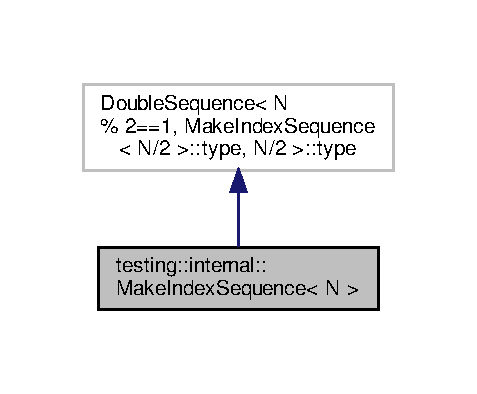
\includegraphics[width=229pt]{structtesting_1_1internal_1_1MakeIndexSequence__inherit__graph}
\end{center}
\end{figure}


Collaboration diagram for testing\+:\+:internal\+:\+:Make\+Index\+Sequence$<$ N $>$\+:\nopagebreak
\begin{figure}[H]
\begin{center}
\leavevmode
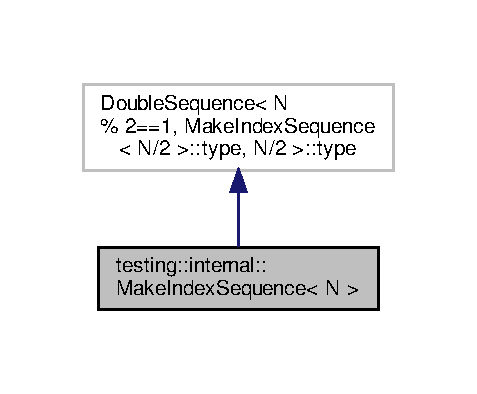
\includegraphics[width=229pt]{structtesting_1_1internal_1_1MakeIndexSequence__coll__graph}
\end{center}
\end{figure}


The documentation for this struct was generated from the following file\+:\begin{DoxyCompactItemize}
\item 
tests/googletest/include/gtest/internal/\hyperlink{gtest-internal_8h}{gtest-\/internal.\+h}\end{DoxyCompactItemize}

\hypertarget{structtesting_1_1internal_1_1MakeIndexSequence_3_010_01_4}{}\section{testing\+:\+:internal\+:\+:Make\+Index\+Sequence$<$ 0 $>$ Struct Template Reference}
\label{structtesting_1_1internal_1_1MakeIndexSequence_3_010_01_4}\index{testing\+::internal\+::\+Make\+Index\+Sequence$<$ 0 $>$@{testing\+::internal\+::\+Make\+Index\+Sequence$<$ 0 $>$}}


{\ttfamily \#include $<$gtest-\/internal.\+h$>$}



Inheritance diagram for testing\+:\+:internal\+:\+:Make\+Index\+Sequence$<$ 0 $>$\+:\nopagebreak
\begin{figure}[H]
\begin{center}
\leavevmode
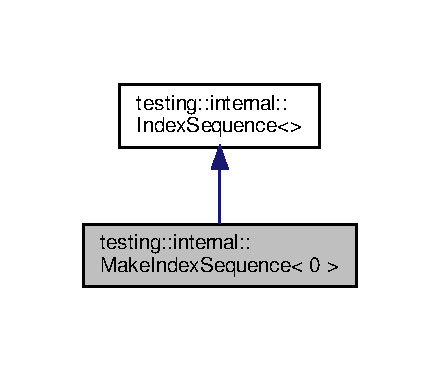
\includegraphics[width=211pt]{structtesting_1_1internal_1_1MakeIndexSequence_3_010_01_4__inherit__graph}
\end{center}
\end{figure}


Collaboration diagram for testing\+:\+:internal\+:\+:Make\+Index\+Sequence$<$ 0 $>$\+:\nopagebreak
\begin{figure}[H]
\begin{center}
\leavevmode
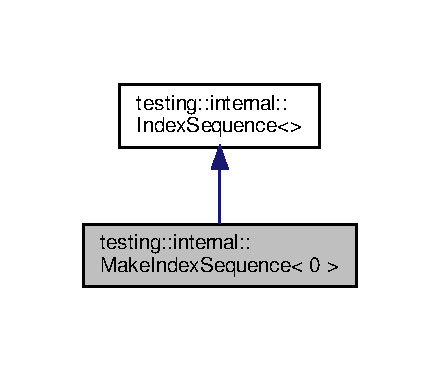
\includegraphics[width=211pt]{structtesting_1_1internal_1_1MakeIndexSequence_3_010_01_4__coll__graph}
\end{center}
\end{figure}
\subsection*{Additional Inherited Members}


The documentation for this struct was generated from the following file\+:\begin{DoxyCompactItemize}
\item 
tests/googletest/include/gtest/internal/\hyperlink{gtest-internal_8h}{gtest-\/internal.\+h}\end{DoxyCompactItemize}

\hypertarget{classtesting_1_1Message}{}\section{testing\+:\+:Message Class Reference}
\label{classtesting_1_1Message}\index{testing\+::\+Message@{testing\+::\+Message}}


{\ttfamily \#include $<$gtest-\/message.\+h$>$}

\subsection*{Public Member Functions}
\begin{DoxyCompactItemize}
\item 
\hyperlink{classtesting_1_1Message_af5ba7216630df9845f18feb64b1a5383}{Message} ()
\item 
\hyperlink{classtesting_1_1Message_ac126e24804817a053bebba0920d94a11}{Message} (const \hyperlink{classtesting_1_1Message}{Message} \&msg)
\item 
\hyperlink{classtesting_1_1Message_a9de694ca239486809fc99fbbea8ac21d}{Message} (const char $\ast$str)
\item 
{\footnotesize template$<$typename T $>$ }\\\hyperlink{classtesting_1_1Message}{Message} \& \hyperlink{classtesting_1_1Message_a2e0e71be52d54c20a75a55fca812721f}{operator$<$$<$} (const T \&val)
\item 
{\footnotesize template$<$typename T $>$ }\\\hyperlink{classtesting_1_1Message}{Message} \& \hyperlink{classtesting_1_1Message_aa3ab685879958f90d2d8cd5b68d10c34}{operator$<$$<$} (T $\ast$const \&pointer)
\item 
\hyperlink{classtesting_1_1Message}{Message} \& \hyperlink{classtesting_1_1Message_a3a71a1c1c8ea52de5852d75483d41453}{operator$<$$<$} (\hyperlink{classtesting_1_1Message_ad398b70e2a11b923cef05c809b0eeb92}{Basic\+Narrow\+Io\+Manip} val)
\item 
\hyperlink{classtesting_1_1Message}{Message} \& \hyperlink{classtesting_1_1Message_a3e1e04f23b1bdfe18adfd59928296346}{operator$<$$<$} (bool b)
\item 
\hyperlink{classtesting_1_1Message}{Message} \& \hyperlink{classtesting_1_1Message_a34774e225944cb6df02db9689d312aae}{operator$<$$<$} (const wchar\+\_\+t $\ast$wide\+\_\+c\+\_\+str)
\item 
\hyperlink{classtesting_1_1Message}{Message} \& \hyperlink{classtesting_1_1Message_aae57eefb3a72a19c11453d630b1d846c}{operator$<$$<$} (wchar\+\_\+t $\ast$wide\+\_\+c\+\_\+str)
\item 
std\+::string \hyperlink{classtesting_1_1Message_a2cdc4df62bdcc9df37651a1cf527704e}{Get\+String} () const
\end{DoxyCompactItemize}
\subsection*{Private Types}
\begin{DoxyCompactItemize}
\item 
typedef std\+::ostream \&($\ast$ \hyperlink{classtesting_1_1Message_ad398b70e2a11b923cef05c809b0eeb92}{Basic\+Narrow\+Io\+Manip}) (std\+::ostream \&)
\end{DoxyCompactItemize}
\subsection*{Private Member Functions}
\begin{DoxyCompactItemize}
\item 
void \hyperlink{classtesting_1_1Message_a5a0462b539ffb88f15ea0c67977774af}{operator=} (const \hyperlink{classtesting_1_1Message}{Message} \&)
\end{DoxyCompactItemize}
\subsection*{Private Attributes}
\begin{DoxyCompactItemize}
\item 
const std\+::unique\+\_\+ptr$<$ \+::std\+::stringstream $>$ \hyperlink{classtesting_1_1Message_a22a52314ba644b1eda454a82ac1fabd8}{ss\+\_\+}
\end{DoxyCompactItemize}


\subsection{Member Typedef Documentation}
\mbox{\Hypertarget{classtesting_1_1Message_ad398b70e2a11b923cef05c809b0eeb92}\label{classtesting_1_1Message_ad398b70e2a11b923cef05c809b0eeb92}} 
\index{testing\+::\+Message@{testing\+::\+Message}!Basic\+Narrow\+Io\+Manip@{Basic\+Narrow\+Io\+Manip}}
\index{Basic\+Narrow\+Io\+Manip@{Basic\+Narrow\+Io\+Manip}!testing\+::\+Message@{testing\+::\+Message}}
\subsubsection{\texorpdfstring{Basic\+Narrow\+Io\+Manip}{BasicNarrowIoManip}}
{\footnotesize\ttfamily typedef std\+::ostream\&($\ast$ testing\+::\+Message\+::\+Basic\+Narrow\+Io\+Manip) (std\+::ostream \&)\hspace{0.3cm}{\ttfamily [private]}}



\subsection{Constructor \& Destructor Documentation}
\mbox{\Hypertarget{classtesting_1_1Message_af5ba7216630df9845f18feb64b1a5383}\label{classtesting_1_1Message_af5ba7216630df9845f18feb64b1a5383}} 
\index{testing\+::\+Message@{testing\+::\+Message}!Message@{Message}}
\index{Message@{Message}!testing\+::\+Message@{testing\+::\+Message}}
\subsubsection{\texorpdfstring{Message()}{Message()}\hspace{0.1cm}{\footnotesize\ttfamily [1/3]}}
{\footnotesize\ttfamily testing\+::\+Message\+::\+Message (\begin{DoxyParamCaption}{ }\end{DoxyParamCaption})}

\mbox{\Hypertarget{classtesting_1_1Message_ac126e24804817a053bebba0920d94a11}\label{classtesting_1_1Message_ac126e24804817a053bebba0920d94a11}} 
\index{testing\+::\+Message@{testing\+::\+Message}!Message@{Message}}
\index{Message@{Message}!testing\+::\+Message@{testing\+::\+Message}}
\subsubsection{\texorpdfstring{Message()}{Message()}\hspace{0.1cm}{\footnotesize\ttfamily [2/3]}}
{\footnotesize\ttfamily testing\+::\+Message\+::\+Message (\begin{DoxyParamCaption}\item[{const \hyperlink{classtesting_1_1Message}{Message} \&}]{msg }\end{DoxyParamCaption})\hspace{0.3cm}{\ttfamily [inline]}}

\mbox{\Hypertarget{classtesting_1_1Message_a9de694ca239486809fc99fbbea8ac21d}\label{classtesting_1_1Message_a9de694ca239486809fc99fbbea8ac21d}} 
\index{testing\+::\+Message@{testing\+::\+Message}!Message@{Message}}
\index{Message@{Message}!testing\+::\+Message@{testing\+::\+Message}}
\subsubsection{\texorpdfstring{Message()}{Message()}\hspace{0.1cm}{\footnotesize\ttfamily [3/3]}}
{\footnotesize\ttfamily testing\+::\+Message\+::\+Message (\begin{DoxyParamCaption}\item[{const char $\ast$}]{str }\end{DoxyParamCaption})\hspace{0.3cm}{\ttfamily [inline]}, {\ttfamily [explicit]}}



\subsection{Member Function Documentation}
\mbox{\Hypertarget{classtesting_1_1Message_a2cdc4df62bdcc9df37651a1cf527704e}\label{classtesting_1_1Message_a2cdc4df62bdcc9df37651a1cf527704e}} 
\index{testing\+::\+Message@{testing\+::\+Message}!Get\+String@{Get\+String}}
\index{Get\+String@{Get\+String}!testing\+::\+Message@{testing\+::\+Message}}
\subsubsection{\texorpdfstring{Get\+String()}{GetString()}}
{\footnotesize\ttfamily std\+::string testing\+::\+Message\+::\+Get\+String (\begin{DoxyParamCaption}{ }\end{DoxyParamCaption}) const}

\mbox{\Hypertarget{classtesting_1_1Message_a2e0e71be52d54c20a75a55fca812721f}\label{classtesting_1_1Message_a2e0e71be52d54c20a75a55fca812721f}} 
\index{testing\+::\+Message@{testing\+::\+Message}!operator$<$$<$@{operator$<$$<$}}
\index{operator$<$$<$@{operator$<$$<$}!testing\+::\+Message@{testing\+::\+Message}}
\subsubsection{\texorpdfstring{operator$<$$<$()}{operator<<()}\hspace{0.1cm}{\footnotesize\ttfamily [1/6]}}
{\footnotesize\ttfamily template$<$typename T $>$ \\
\hyperlink{classtesting_1_1Message}{Message}\& testing\+::\+Message\+::operator$<$$<$ (\begin{DoxyParamCaption}\item[{const T \&}]{val }\end{DoxyParamCaption})\hspace{0.3cm}{\ttfamily [inline]}}

\mbox{\Hypertarget{classtesting_1_1Message_aa3ab685879958f90d2d8cd5b68d10c34}\label{classtesting_1_1Message_aa3ab685879958f90d2d8cd5b68d10c34}} 
\index{testing\+::\+Message@{testing\+::\+Message}!operator$<$$<$@{operator$<$$<$}}
\index{operator$<$$<$@{operator$<$$<$}!testing\+::\+Message@{testing\+::\+Message}}
\subsubsection{\texorpdfstring{operator$<$$<$()}{operator<<()}\hspace{0.1cm}{\footnotesize\ttfamily [2/6]}}
{\footnotesize\ttfamily template$<$typename T $>$ \\
\hyperlink{classtesting_1_1Message}{Message}\& testing\+::\+Message\+::operator$<$$<$ (\begin{DoxyParamCaption}\item[{T $\ast$const \&}]{pointer }\end{DoxyParamCaption})\hspace{0.3cm}{\ttfamily [inline]}}

\mbox{\Hypertarget{classtesting_1_1Message_a3a71a1c1c8ea52de5852d75483d41453}\label{classtesting_1_1Message_a3a71a1c1c8ea52de5852d75483d41453}} 
\index{testing\+::\+Message@{testing\+::\+Message}!operator$<$$<$@{operator$<$$<$}}
\index{operator$<$$<$@{operator$<$$<$}!testing\+::\+Message@{testing\+::\+Message}}
\subsubsection{\texorpdfstring{operator$<$$<$()}{operator<<()}\hspace{0.1cm}{\footnotesize\ttfamily [3/6]}}
{\footnotesize\ttfamily \hyperlink{classtesting_1_1Message}{Message}\& testing\+::\+Message\+::operator$<$$<$ (\begin{DoxyParamCaption}\item[{\hyperlink{classtesting_1_1Message_ad398b70e2a11b923cef05c809b0eeb92}{Basic\+Narrow\+Io\+Manip}}]{val }\end{DoxyParamCaption})\hspace{0.3cm}{\ttfamily [inline]}}

\mbox{\Hypertarget{classtesting_1_1Message_a3e1e04f23b1bdfe18adfd59928296346}\label{classtesting_1_1Message_a3e1e04f23b1bdfe18adfd59928296346}} 
\index{testing\+::\+Message@{testing\+::\+Message}!operator$<$$<$@{operator$<$$<$}}
\index{operator$<$$<$@{operator$<$$<$}!testing\+::\+Message@{testing\+::\+Message}}
\subsubsection{\texorpdfstring{operator$<$$<$()}{operator<<()}\hspace{0.1cm}{\footnotesize\ttfamily [4/6]}}
{\footnotesize\ttfamily \hyperlink{classtesting_1_1Message}{Message}\& testing\+::\+Message\+::operator$<$$<$ (\begin{DoxyParamCaption}\item[{bool}]{b }\end{DoxyParamCaption})\hspace{0.3cm}{\ttfamily [inline]}}

\mbox{\Hypertarget{classtesting_1_1Message_a34774e225944cb6df02db9689d312aae}\label{classtesting_1_1Message_a34774e225944cb6df02db9689d312aae}} 
\index{testing\+::\+Message@{testing\+::\+Message}!operator$<$$<$@{operator$<$$<$}}
\index{operator$<$$<$@{operator$<$$<$}!testing\+::\+Message@{testing\+::\+Message}}
\subsubsection{\texorpdfstring{operator$<$$<$()}{operator<<()}\hspace{0.1cm}{\footnotesize\ttfamily [5/6]}}
{\footnotesize\ttfamily \hyperlink{classtesting_1_1Message}{Message}\& testing\+::\+Message\+::operator$<$$<$ (\begin{DoxyParamCaption}\item[{const wchar\+\_\+t $\ast$}]{wide\+\_\+c\+\_\+str }\end{DoxyParamCaption})}

\mbox{\Hypertarget{classtesting_1_1Message_aae57eefb3a72a19c11453d630b1d846c}\label{classtesting_1_1Message_aae57eefb3a72a19c11453d630b1d846c}} 
\index{testing\+::\+Message@{testing\+::\+Message}!operator$<$$<$@{operator$<$$<$}}
\index{operator$<$$<$@{operator$<$$<$}!testing\+::\+Message@{testing\+::\+Message}}
\subsubsection{\texorpdfstring{operator$<$$<$()}{operator<<()}\hspace{0.1cm}{\footnotesize\ttfamily [6/6]}}
{\footnotesize\ttfamily \hyperlink{classtesting_1_1Message}{Message}\& testing\+::\+Message\+::operator$<$$<$ (\begin{DoxyParamCaption}\item[{wchar\+\_\+t $\ast$}]{wide\+\_\+c\+\_\+str }\end{DoxyParamCaption})}

\mbox{\Hypertarget{classtesting_1_1Message_a5a0462b539ffb88f15ea0c67977774af}\label{classtesting_1_1Message_a5a0462b539ffb88f15ea0c67977774af}} 
\index{testing\+::\+Message@{testing\+::\+Message}!operator=@{operator=}}
\index{operator=@{operator=}!testing\+::\+Message@{testing\+::\+Message}}
\subsubsection{\texorpdfstring{operator=()}{operator=()}}
{\footnotesize\ttfamily void testing\+::\+Message\+::operator= (\begin{DoxyParamCaption}\item[{const \hyperlink{classtesting_1_1Message}{Message} \&}]{ }\end{DoxyParamCaption})\hspace{0.3cm}{\ttfamily [private]}}



\subsection{Member Data Documentation}
\mbox{\Hypertarget{classtesting_1_1Message_a22a52314ba644b1eda454a82ac1fabd8}\label{classtesting_1_1Message_a22a52314ba644b1eda454a82ac1fabd8}} 
\index{testing\+::\+Message@{testing\+::\+Message}!ss\+\_\+@{ss\+\_\+}}
\index{ss\+\_\+@{ss\+\_\+}!testing\+::\+Message@{testing\+::\+Message}}
\subsubsection{\texorpdfstring{ss\+\_\+}{ss\_}}
{\footnotesize\ttfamily const std\+::unique\+\_\+ptr$<$ \+::std\+::stringstream$>$ testing\+::\+Message\+::ss\+\_\+\hspace{0.3cm}{\ttfamily [private]}}



The documentation for this class was generated from the following file\+:\begin{DoxyCompactItemize}
\item 
tests/googletest/include/gtest/\hyperlink{gtest-message_8h}{gtest-\/message.\+h}\end{DoxyCompactItemize}

\hypertarget{classtesting_1_1internal_1_1Mutex}{}\section{testing\+:\+:internal\+:\+:Mutex Class Reference}
\label{classtesting_1_1internal_1_1Mutex}\index{testing\+::internal\+::\+Mutex@{testing\+::internal\+::\+Mutex}}


{\ttfamily \#include $<$gtest-\/port.\+h$>$}

\subsection*{Public Member Functions}
\begin{DoxyCompactItemize}
\item 
\hyperlink{classtesting_1_1internal_1_1Mutex_a38e1833a78e3eec81ad23ce1b056b40e}{Mutex} ()
\item 
void \hyperlink{classtesting_1_1internal_1_1Mutex_ae7e2191886c00182176b23c4f4d049f8}{Lock} ()
\item 
void \hyperlink{classtesting_1_1internal_1_1Mutex_a315188055de1be98884519ad84eff2e6}{Unlock} ()
\item 
void \hyperlink{classtesting_1_1internal_1_1Mutex_af45bf1660ac4110338a02a8680b2f486}{Assert\+Held} () const
\end{DoxyCompactItemize}


\subsection{Constructor \& Destructor Documentation}
\mbox{\Hypertarget{classtesting_1_1internal_1_1Mutex_a38e1833a78e3eec81ad23ce1b056b40e}\label{classtesting_1_1internal_1_1Mutex_a38e1833a78e3eec81ad23ce1b056b40e}} 
\index{testing\+::internal\+::\+Mutex@{testing\+::internal\+::\+Mutex}!Mutex@{Mutex}}
\index{Mutex@{Mutex}!testing\+::internal\+::\+Mutex@{testing\+::internal\+::\+Mutex}}
\subsubsection{\texorpdfstring{Mutex()}{Mutex()}}
{\footnotesize\ttfamily testing\+::internal\+::\+Mutex\+::\+Mutex (\begin{DoxyParamCaption}{ }\end{DoxyParamCaption})\hspace{0.3cm}{\ttfamily [inline]}}



\subsection{Member Function Documentation}
\mbox{\Hypertarget{classtesting_1_1internal_1_1Mutex_af45bf1660ac4110338a02a8680b2f486}\label{classtesting_1_1internal_1_1Mutex_af45bf1660ac4110338a02a8680b2f486}} 
\index{testing\+::internal\+::\+Mutex@{testing\+::internal\+::\+Mutex}!Assert\+Held@{Assert\+Held}}
\index{Assert\+Held@{Assert\+Held}!testing\+::internal\+::\+Mutex@{testing\+::internal\+::\+Mutex}}
\subsubsection{\texorpdfstring{Assert\+Held()}{AssertHeld()}}
{\footnotesize\ttfamily void testing\+::internal\+::\+Mutex\+::\+Assert\+Held (\begin{DoxyParamCaption}{ }\end{DoxyParamCaption}) const\hspace{0.3cm}{\ttfamily [inline]}}

\mbox{\Hypertarget{classtesting_1_1internal_1_1Mutex_ae7e2191886c00182176b23c4f4d049f8}\label{classtesting_1_1internal_1_1Mutex_ae7e2191886c00182176b23c4f4d049f8}} 
\index{testing\+::internal\+::\+Mutex@{testing\+::internal\+::\+Mutex}!Lock@{Lock}}
\index{Lock@{Lock}!testing\+::internal\+::\+Mutex@{testing\+::internal\+::\+Mutex}}
\subsubsection{\texorpdfstring{Lock()}{Lock()}}
{\footnotesize\ttfamily void testing\+::internal\+::\+Mutex\+::\+Lock (\begin{DoxyParamCaption}{ }\end{DoxyParamCaption})\hspace{0.3cm}{\ttfamily [inline]}}

\mbox{\Hypertarget{classtesting_1_1internal_1_1Mutex_a315188055de1be98884519ad84eff2e6}\label{classtesting_1_1internal_1_1Mutex_a315188055de1be98884519ad84eff2e6}} 
\index{testing\+::internal\+::\+Mutex@{testing\+::internal\+::\+Mutex}!Unlock@{Unlock}}
\index{Unlock@{Unlock}!testing\+::internal\+::\+Mutex@{testing\+::internal\+::\+Mutex}}
\subsubsection{\texorpdfstring{Unlock()}{Unlock()}}
{\footnotesize\ttfamily void testing\+::internal\+::\+Mutex\+::\+Unlock (\begin{DoxyParamCaption}{ }\end{DoxyParamCaption})\hspace{0.3cm}{\ttfamily [inline]}}



The documentation for this class was generated from the following file\+:\begin{DoxyCompactItemize}
\item 
tests/googletest/include/gtest/internal/\hyperlink{gtest-port_8h}{gtest-\/port.\+h}\end{DoxyCompactItemize}

\hypertarget{classMyString}{}\section{My\+String Class Reference}
\label{classMyString}\index{My\+String@{My\+String}}


{\ttfamily \#include $<$sample2.\+h$>$}

\subsection*{Public Member Functions}
\begin{DoxyCompactItemize}
\item 
\hyperlink{classMyString_a1cb17852b83614394b59720779c5f918}{My\+String} ()
\item 
\hyperlink{classMyString_a28134eb91b6698f46b12accefa157d0f}{My\+String} (const char $\ast$a\+\_\+c\+\_\+string)
\item 
\hyperlink{classMyString_ae24c7cf89a58dd2287303df2ac054c66}{My\+String} (const \hyperlink{classMyString}{My\+String} \&string)
\item 
\hyperlink{classMyString_a7bee4fe8ad82a0b7b8f65b02054b156b}{$\sim$\+My\+String} ()
\item 
const char $\ast$ \hyperlink{classMyString_aff2af0cf30db39fe24a235670ee6ff25}{c\+\_\+string} () const
\item 
size\+\_\+t \hyperlink{classMyString_a4eb168b1ec401a732b3859abe004d648}{Length} () const
\item 
void \hyperlink{classMyString_a521c4cd7eccac6ce554d8a51505e4970}{Set} (const char $\ast$\hyperlink{classMyString_aff2af0cf30db39fe24a235670ee6ff25}{c\+\_\+string})
\end{DoxyCompactItemize}
\subsection*{Static Public Member Functions}
\begin{DoxyCompactItemize}
\item 
static const char $\ast$ \hyperlink{classMyString_a3acde3db40f8e70bad239739a5466275}{Clone\+C\+String} (const char $\ast$a\+\_\+c\+\_\+string)
\end{DoxyCompactItemize}
\subsection*{Private Member Functions}
\begin{DoxyCompactItemize}
\item 
const \hyperlink{classMyString}{My\+String} \& \hyperlink{classMyString_a0156d24764b9d8e4303763750f95cd38}{operator=} (const \hyperlink{classMyString}{My\+String} \&rhs)
\end{DoxyCompactItemize}
\subsection*{Private Attributes}
\begin{DoxyCompactItemize}
\item 
const char $\ast$ \hyperlink{classMyString_a1872c0d04ff5f6e654161472b18bb9d0}{c\+\_\+string\+\_\+}
\end{DoxyCompactItemize}


\subsection{Constructor \& Destructor Documentation}
\mbox{\Hypertarget{classMyString_a1cb17852b83614394b59720779c5f918}\label{classMyString_a1cb17852b83614394b59720779c5f918}} 
\index{My\+String@{My\+String}!My\+String@{My\+String}}
\index{My\+String@{My\+String}!My\+String@{My\+String}}
\subsubsection{\texorpdfstring{My\+String()}{MyString()}\hspace{0.1cm}{\footnotesize\ttfamily [1/3]}}
{\footnotesize\ttfamily My\+String\+::\+My\+String (\begin{DoxyParamCaption}{ }\end{DoxyParamCaption})\hspace{0.3cm}{\ttfamily [inline]}}

\mbox{\Hypertarget{classMyString_a28134eb91b6698f46b12accefa157d0f}\label{classMyString_a28134eb91b6698f46b12accefa157d0f}} 
\index{My\+String@{My\+String}!My\+String@{My\+String}}
\index{My\+String@{My\+String}!My\+String@{My\+String}}
\subsubsection{\texorpdfstring{My\+String()}{MyString()}\hspace{0.1cm}{\footnotesize\ttfamily [2/3]}}
{\footnotesize\ttfamily My\+String\+::\+My\+String (\begin{DoxyParamCaption}\item[{const char $\ast$}]{a\+\_\+c\+\_\+string }\end{DoxyParamCaption})\hspace{0.3cm}{\ttfamily [inline]}, {\ttfamily [explicit]}}

\mbox{\Hypertarget{classMyString_ae24c7cf89a58dd2287303df2ac054c66}\label{classMyString_ae24c7cf89a58dd2287303df2ac054c66}} 
\index{My\+String@{My\+String}!My\+String@{My\+String}}
\index{My\+String@{My\+String}!My\+String@{My\+String}}
\subsubsection{\texorpdfstring{My\+String()}{MyString()}\hspace{0.1cm}{\footnotesize\ttfamily [3/3]}}
{\footnotesize\ttfamily My\+String\+::\+My\+String (\begin{DoxyParamCaption}\item[{const \hyperlink{classMyString}{My\+String} \&}]{string }\end{DoxyParamCaption})\hspace{0.3cm}{\ttfamily [inline]}}

\mbox{\Hypertarget{classMyString_a7bee4fe8ad82a0b7b8f65b02054b156b}\label{classMyString_a7bee4fe8ad82a0b7b8f65b02054b156b}} 
\index{My\+String@{My\+String}!````~My\+String@{$\sim$\+My\+String}}
\index{````~My\+String@{$\sim$\+My\+String}!My\+String@{My\+String}}
\subsubsection{\texorpdfstring{$\sim$\+My\+String()}{~MyString()}}
{\footnotesize\ttfamily My\+String\+::$\sim$\+My\+String (\begin{DoxyParamCaption}{ }\end{DoxyParamCaption})\hspace{0.3cm}{\ttfamily [inline]}}



\subsection{Member Function Documentation}
\mbox{\Hypertarget{classMyString_aff2af0cf30db39fe24a235670ee6ff25}\label{classMyString_aff2af0cf30db39fe24a235670ee6ff25}} 
\index{My\+String@{My\+String}!c\+\_\+string@{c\+\_\+string}}
\index{c\+\_\+string@{c\+\_\+string}!My\+String@{My\+String}}
\subsubsection{\texorpdfstring{c\+\_\+string()}{c\_string()}}
{\footnotesize\ttfamily const char$\ast$ My\+String\+::c\+\_\+string (\begin{DoxyParamCaption}{ }\end{DoxyParamCaption}) const\hspace{0.3cm}{\ttfamily [inline]}}

\mbox{\Hypertarget{classMyString_a3acde3db40f8e70bad239739a5466275}\label{classMyString_a3acde3db40f8e70bad239739a5466275}} 
\index{My\+String@{My\+String}!Clone\+C\+String@{Clone\+C\+String}}
\index{Clone\+C\+String@{Clone\+C\+String}!My\+String@{My\+String}}
\subsubsection{\texorpdfstring{Clone\+C\+String()}{CloneCString()}}
{\footnotesize\ttfamily static const char$\ast$ My\+String\+::\+Clone\+C\+String (\begin{DoxyParamCaption}\item[{const char $\ast$}]{a\+\_\+c\+\_\+string }\end{DoxyParamCaption})\hspace{0.3cm}{\ttfamily [static]}}

\mbox{\Hypertarget{classMyString_a4eb168b1ec401a732b3859abe004d648}\label{classMyString_a4eb168b1ec401a732b3859abe004d648}} 
\index{My\+String@{My\+String}!Length@{Length}}
\index{Length@{Length}!My\+String@{My\+String}}
\subsubsection{\texorpdfstring{Length()}{Length()}}
{\footnotesize\ttfamily size\+\_\+t My\+String\+::\+Length (\begin{DoxyParamCaption}{ }\end{DoxyParamCaption}) const\hspace{0.3cm}{\ttfamily [inline]}}

\mbox{\Hypertarget{classMyString_a0156d24764b9d8e4303763750f95cd38}\label{classMyString_a0156d24764b9d8e4303763750f95cd38}} 
\index{My\+String@{My\+String}!operator=@{operator=}}
\index{operator=@{operator=}!My\+String@{My\+String}}
\subsubsection{\texorpdfstring{operator=()}{operator=()}}
{\footnotesize\ttfamily const \hyperlink{classMyString}{My\+String}\& My\+String\+::operator= (\begin{DoxyParamCaption}\item[{const \hyperlink{classMyString}{My\+String} \&}]{rhs }\end{DoxyParamCaption})\hspace{0.3cm}{\ttfamily [private]}}

\mbox{\Hypertarget{classMyString_a521c4cd7eccac6ce554d8a51505e4970}\label{classMyString_a521c4cd7eccac6ce554d8a51505e4970}} 
\index{My\+String@{My\+String}!Set@{Set}}
\index{Set@{Set}!My\+String@{My\+String}}
\subsubsection{\texorpdfstring{Set()}{Set()}}
{\footnotesize\ttfamily void My\+String\+::\+Set (\begin{DoxyParamCaption}\item[{const char $\ast$}]{c\+\_\+string }\end{DoxyParamCaption})}



\subsection{Member Data Documentation}
\mbox{\Hypertarget{classMyString_a1872c0d04ff5f6e654161472b18bb9d0}\label{classMyString_a1872c0d04ff5f6e654161472b18bb9d0}} 
\index{My\+String@{My\+String}!c\+\_\+string\+\_\+@{c\+\_\+string\+\_\+}}
\index{c\+\_\+string\+\_\+@{c\+\_\+string\+\_\+}!My\+String@{My\+String}}
\subsubsection{\texorpdfstring{c\+\_\+string\+\_\+}{c\_string\_}}
{\footnotesize\ttfamily const char$\ast$ My\+String\+::c\+\_\+string\+\_\+\hspace{0.3cm}{\ttfamily [private]}}



The documentation for this class was generated from the following file\+:\begin{DoxyCompactItemize}
\item 
tests/googletest/samples/\hyperlink{sample2_8h}{sample2.\+h}\end{DoxyCompactItemize}

\hypertarget{classtesting_1_1internal_1_1NativeArray}{}\section{testing\+:\+:internal\+:\+:Native\+Array$<$ Element $>$ Class Template Reference}
\label{classtesting_1_1internal_1_1NativeArray}\index{testing\+::internal\+::\+Native\+Array$<$ Element $>$@{testing\+::internal\+::\+Native\+Array$<$ Element $>$}}


{\ttfamily \#include $<$gtest-\/internal.\+h$>$}

\subsection*{Public Types}
\begin{DoxyCompactItemize}
\item 
typedef Element \hyperlink{classtesting_1_1internal_1_1NativeArray_a12216d686e16e4cc63d952fada5b2ba9}{value\+\_\+type}
\item 
typedef Element $\ast$ \hyperlink{classtesting_1_1internal_1_1NativeArray_ac1301a57977b57a1ad013e4e25fc2a72}{iterator}
\item 
typedef const Element $\ast$ \hyperlink{classtesting_1_1internal_1_1NativeArray_a9ce7c8408460d7158a2870456d134557}{const\+\_\+iterator}
\end{DoxyCompactItemize}
\subsection*{Public Member Functions}
\begin{DoxyCompactItemize}
\item 
\hyperlink{classtesting_1_1internal_1_1NativeArray_a52b3689c62532703d11e9d82939a7141}{Native\+Array} (const Element $\ast$array, size\+\_\+t count, \hyperlink{structtesting_1_1internal_1_1RelationToSourceReference}{Relation\+To\+Source\+Reference})
\item 
\hyperlink{classtesting_1_1internal_1_1NativeArray_ac184ee5741af5be3402213819c834405}{Native\+Array} (const Element $\ast$array, size\+\_\+t count, \hyperlink{structtesting_1_1internal_1_1RelationToSourceCopy}{Relation\+To\+Source\+Copy})
\item 
\hyperlink{classtesting_1_1internal_1_1NativeArray_abb346ac3040f5da733f594cc2d5958bc}{Native\+Array} (const \hyperlink{classtesting_1_1internal_1_1NativeArray}{Native\+Array} \&rhs)
\item 
\hyperlink{classtesting_1_1internal_1_1NativeArray_a55ab5948d473a487303dcf6e02ad1f60}{$\sim$\+Native\+Array} ()
\item 
size\+\_\+t \hyperlink{classtesting_1_1internal_1_1NativeArray_af96a4a5ca0cdd5d163c47a081f08bd89}{size} () const
\item 
\hyperlink{classtesting_1_1internal_1_1NativeArray_a9ce7c8408460d7158a2870456d134557}{const\+\_\+iterator} \hyperlink{classtesting_1_1internal_1_1NativeArray_a3046d93cfa23097e7b7c91f5f982dc78}{begin} () const
\item 
\hyperlink{classtesting_1_1internal_1_1NativeArray_a9ce7c8408460d7158a2870456d134557}{const\+\_\+iterator} \hyperlink{classtesting_1_1internal_1_1NativeArray_ae1cda748e49c6906421c6183c4d07c5a}{end} () const
\item 
bool \hyperlink{classtesting_1_1internal_1_1NativeArray_a81b90f5739ed812610e68dc34c9e3850}{operator==} (const \hyperlink{classtesting_1_1internal_1_1NativeArray}{Native\+Array} \&rhs) const
\end{DoxyCompactItemize}
\subsection*{Private Types}
\begin{DoxyCompactItemize}
\item 
enum \{ \hyperlink{classtesting_1_1internal_1_1NativeArray_abe36a7e1b487dc6b9bd81489b1c2af28a3be52e24b6c1558a819baf99922f9296}{k\+Check\+Type\+Is\+Not\+Const\+Or\+A\+Reference}
 \}
\end{DoxyCompactItemize}
\subsection*{Private Member Functions}
\begin{DoxyCompactItemize}
\item 
void \hyperlink{classtesting_1_1internal_1_1NativeArray_a8c0069cc09f559785fe4923fc118056f}{Init\+Copy} (const Element $\ast$array, size\+\_\+t a\+\_\+size)
\item 
void \hyperlink{classtesting_1_1internal_1_1NativeArray_ac6ad6d79e17e2c98a9d4d684afcb7f79}{Init\+Ref} (const Element $\ast$array, size\+\_\+t a\+\_\+size)
\item 
\hyperlink{classtesting_1_1internal_1_1NativeArray_a6633f3eab6947d4502fb1c69f95be66e}{G\+T\+E\+S\+T\+\_\+\+D\+I\+S\+A\+L\+L\+O\+W\+\_\+\+A\+S\+S\+I\+G\+N\+\_\+} (\hyperlink{classtesting_1_1internal_1_1NativeArray}{Native\+Array})
\end{DoxyCompactItemize}
\subsection*{Private Attributes}
\begin{DoxyCompactItemize}
\item 
const Element $\ast$ \hyperlink{classtesting_1_1internal_1_1NativeArray_adadc025fbbbd43904d4036991019f18f}{array\+\_\+}
\item 
size\+\_\+t \hyperlink{classtesting_1_1internal_1_1NativeArray_aa7e4251de39aaa75f697f0eaeedbf06e}{size\+\_\+}
\item 
void(Native\+Array\+::$\ast$ \hyperlink{classtesting_1_1internal_1_1NativeArray_addd7442a10398a60215a9989bcbd8078}{clone\+\_\+} )(const Element $\ast$, size\+\_\+t)
\end{DoxyCompactItemize}


\subsection{Member Typedef Documentation}
\mbox{\Hypertarget{classtesting_1_1internal_1_1NativeArray_a9ce7c8408460d7158a2870456d134557}\label{classtesting_1_1internal_1_1NativeArray_a9ce7c8408460d7158a2870456d134557}} 
\index{testing\+::internal\+::\+Native\+Array@{testing\+::internal\+::\+Native\+Array}!const\+\_\+iterator@{const\+\_\+iterator}}
\index{const\+\_\+iterator@{const\+\_\+iterator}!testing\+::internal\+::\+Native\+Array@{testing\+::internal\+::\+Native\+Array}}
\subsubsection{\texorpdfstring{const\+\_\+iterator}{const\_iterator}}
{\footnotesize\ttfamily template$<$typename Element $>$ \\
typedef const Element$\ast$ \hyperlink{classtesting_1_1internal_1_1NativeArray}{testing\+::internal\+::\+Native\+Array}$<$ Element $>$\+::\hyperlink{classtesting_1_1internal_1_1NativeArray_a9ce7c8408460d7158a2870456d134557}{const\+\_\+iterator}}

\mbox{\Hypertarget{classtesting_1_1internal_1_1NativeArray_ac1301a57977b57a1ad013e4e25fc2a72}\label{classtesting_1_1internal_1_1NativeArray_ac1301a57977b57a1ad013e4e25fc2a72}} 
\index{testing\+::internal\+::\+Native\+Array@{testing\+::internal\+::\+Native\+Array}!iterator@{iterator}}
\index{iterator@{iterator}!testing\+::internal\+::\+Native\+Array@{testing\+::internal\+::\+Native\+Array}}
\subsubsection{\texorpdfstring{iterator}{iterator}}
{\footnotesize\ttfamily template$<$typename Element $>$ \\
typedef Element$\ast$ \hyperlink{classtesting_1_1internal_1_1NativeArray}{testing\+::internal\+::\+Native\+Array}$<$ Element $>$\+::\hyperlink{classtesting_1_1internal_1_1NativeArray_ac1301a57977b57a1ad013e4e25fc2a72}{iterator}}

\mbox{\Hypertarget{classtesting_1_1internal_1_1NativeArray_a12216d686e16e4cc63d952fada5b2ba9}\label{classtesting_1_1internal_1_1NativeArray_a12216d686e16e4cc63d952fada5b2ba9}} 
\index{testing\+::internal\+::\+Native\+Array@{testing\+::internal\+::\+Native\+Array}!value\+\_\+type@{value\+\_\+type}}
\index{value\+\_\+type@{value\+\_\+type}!testing\+::internal\+::\+Native\+Array@{testing\+::internal\+::\+Native\+Array}}
\subsubsection{\texorpdfstring{value\+\_\+type}{value\_type}}
{\footnotesize\ttfamily template$<$typename Element $>$ \\
typedef Element \hyperlink{classtesting_1_1internal_1_1NativeArray}{testing\+::internal\+::\+Native\+Array}$<$ Element $>$\+::\hyperlink{classtesting_1_1internal_1_1NativeArray_a12216d686e16e4cc63d952fada5b2ba9}{value\+\_\+type}}



\subsection{Member Enumeration Documentation}
\mbox{\Hypertarget{classtesting_1_1internal_1_1NativeArray_abe36a7e1b487dc6b9bd81489b1c2af28}\label{classtesting_1_1internal_1_1NativeArray_abe36a7e1b487dc6b9bd81489b1c2af28}} 
\subsubsection{\texorpdfstring{anonymous enum}{anonymous enum}}
{\footnotesize\ttfamily template$<$typename Element $>$ \\
anonymous enum\hspace{0.3cm}{\ttfamily [private]}}

\begin{DoxyEnumFields}{Enumerator}
\raisebox{\heightof{T}}[0pt][0pt]{\index{k\+Check\+Type\+Is\+Not\+Const\+Or\+A\+Reference@{k\+Check\+Type\+Is\+Not\+Const\+Or\+A\+Reference}!testing\+::internal\+::\+Native\+Array@{testing\+::internal\+::\+Native\+Array}}\index{testing\+::internal\+::\+Native\+Array@{testing\+::internal\+::\+Native\+Array}!k\+Check\+Type\+Is\+Not\+Const\+Or\+A\+Reference@{k\+Check\+Type\+Is\+Not\+Const\+Or\+A\+Reference}}}\mbox{\Hypertarget{classtesting_1_1internal_1_1NativeArray_abe36a7e1b487dc6b9bd81489b1c2af28a3be52e24b6c1558a819baf99922f9296}\label{classtesting_1_1internal_1_1NativeArray_abe36a7e1b487dc6b9bd81489b1c2af28a3be52e24b6c1558a819baf99922f9296}} 
k\+Check\+Type\+Is\+Not\+Const\+Or\+A\+Reference&\\
\hline

\end{DoxyEnumFields}


\subsection{Constructor \& Destructor Documentation}
\mbox{\Hypertarget{classtesting_1_1internal_1_1NativeArray_a52b3689c62532703d11e9d82939a7141}\label{classtesting_1_1internal_1_1NativeArray_a52b3689c62532703d11e9d82939a7141}} 
\index{testing\+::internal\+::\+Native\+Array@{testing\+::internal\+::\+Native\+Array}!Native\+Array@{Native\+Array}}
\index{Native\+Array@{Native\+Array}!testing\+::internal\+::\+Native\+Array@{testing\+::internal\+::\+Native\+Array}}
\subsubsection{\texorpdfstring{Native\+Array()}{NativeArray()}\hspace{0.1cm}{\footnotesize\ttfamily [1/3]}}
{\footnotesize\ttfamily template$<$typename Element $>$ \\
\hyperlink{classtesting_1_1internal_1_1NativeArray}{testing\+::internal\+::\+Native\+Array}$<$ Element $>$\+::\hyperlink{classtesting_1_1internal_1_1NativeArray}{Native\+Array} (\begin{DoxyParamCaption}\item[{const Element $\ast$}]{array,  }\item[{size\+\_\+t}]{count,  }\item[{\hyperlink{structtesting_1_1internal_1_1RelationToSourceReference}{Relation\+To\+Source\+Reference}}]{ }\end{DoxyParamCaption})\hspace{0.3cm}{\ttfamily [inline]}}

\mbox{\Hypertarget{classtesting_1_1internal_1_1NativeArray_ac184ee5741af5be3402213819c834405}\label{classtesting_1_1internal_1_1NativeArray_ac184ee5741af5be3402213819c834405}} 
\index{testing\+::internal\+::\+Native\+Array@{testing\+::internal\+::\+Native\+Array}!Native\+Array@{Native\+Array}}
\index{Native\+Array@{Native\+Array}!testing\+::internal\+::\+Native\+Array@{testing\+::internal\+::\+Native\+Array}}
\subsubsection{\texorpdfstring{Native\+Array()}{NativeArray()}\hspace{0.1cm}{\footnotesize\ttfamily [2/3]}}
{\footnotesize\ttfamily template$<$typename Element $>$ \\
\hyperlink{classtesting_1_1internal_1_1NativeArray}{testing\+::internal\+::\+Native\+Array}$<$ Element $>$\+::\hyperlink{classtesting_1_1internal_1_1NativeArray}{Native\+Array} (\begin{DoxyParamCaption}\item[{const Element $\ast$}]{array,  }\item[{size\+\_\+t}]{count,  }\item[{\hyperlink{structtesting_1_1internal_1_1RelationToSourceCopy}{Relation\+To\+Source\+Copy}}]{ }\end{DoxyParamCaption})\hspace{0.3cm}{\ttfamily [inline]}}

\mbox{\Hypertarget{classtesting_1_1internal_1_1NativeArray_abb346ac3040f5da733f594cc2d5958bc}\label{classtesting_1_1internal_1_1NativeArray_abb346ac3040f5da733f594cc2d5958bc}} 
\index{testing\+::internal\+::\+Native\+Array@{testing\+::internal\+::\+Native\+Array}!Native\+Array@{Native\+Array}}
\index{Native\+Array@{Native\+Array}!testing\+::internal\+::\+Native\+Array@{testing\+::internal\+::\+Native\+Array}}
\subsubsection{\texorpdfstring{Native\+Array()}{NativeArray()}\hspace{0.1cm}{\footnotesize\ttfamily [3/3]}}
{\footnotesize\ttfamily template$<$typename Element $>$ \\
\hyperlink{classtesting_1_1internal_1_1NativeArray}{testing\+::internal\+::\+Native\+Array}$<$ Element $>$\+::\hyperlink{classtesting_1_1internal_1_1NativeArray}{Native\+Array} (\begin{DoxyParamCaption}\item[{const \hyperlink{classtesting_1_1internal_1_1NativeArray}{Native\+Array}$<$ Element $>$ \&}]{rhs }\end{DoxyParamCaption})\hspace{0.3cm}{\ttfamily [inline]}}

\mbox{\Hypertarget{classtesting_1_1internal_1_1NativeArray_a55ab5948d473a487303dcf6e02ad1f60}\label{classtesting_1_1internal_1_1NativeArray_a55ab5948d473a487303dcf6e02ad1f60}} 
\index{testing\+::internal\+::\+Native\+Array@{testing\+::internal\+::\+Native\+Array}!````~Native\+Array@{$\sim$\+Native\+Array}}
\index{````~Native\+Array@{$\sim$\+Native\+Array}!testing\+::internal\+::\+Native\+Array@{testing\+::internal\+::\+Native\+Array}}
\subsubsection{\texorpdfstring{$\sim$\+Native\+Array()}{~NativeArray()}}
{\footnotesize\ttfamily template$<$typename Element $>$ \\
\hyperlink{classtesting_1_1internal_1_1NativeArray}{testing\+::internal\+::\+Native\+Array}$<$ Element $>$\+::$\sim$\hyperlink{classtesting_1_1internal_1_1NativeArray}{Native\+Array} (\begin{DoxyParamCaption}{ }\end{DoxyParamCaption})\hspace{0.3cm}{\ttfamily [inline]}}



\subsection{Member Function Documentation}
\mbox{\Hypertarget{classtesting_1_1internal_1_1NativeArray_a3046d93cfa23097e7b7c91f5f982dc78}\label{classtesting_1_1internal_1_1NativeArray_a3046d93cfa23097e7b7c91f5f982dc78}} 
\index{testing\+::internal\+::\+Native\+Array@{testing\+::internal\+::\+Native\+Array}!begin@{begin}}
\index{begin@{begin}!testing\+::internal\+::\+Native\+Array@{testing\+::internal\+::\+Native\+Array}}
\subsubsection{\texorpdfstring{begin()}{begin()}}
{\footnotesize\ttfamily template$<$typename Element $>$ \\
\hyperlink{classtesting_1_1internal_1_1NativeArray_a9ce7c8408460d7158a2870456d134557}{const\+\_\+iterator} \hyperlink{classtesting_1_1internal_1_1NativeArray}{testing\+::internal\+::\+Native\+Array}$<$ Element $>$\+::begin (\begin{DoxyParamCaption}{ }\end{DoxyParamCaption}) const\hspace{0.3cm}{\ttfamily [inline]}}

\mbox{\Hypertarget{classtesting_1_1internal_1_1NativeArray_ae1cda748e49c6906421c6183c4d07c5a}\label{classtesting_1_1internal_1_1NativeArray_ae1cda748e49c6906421c6183c4d07c5a}} 
\index{testing\+::internal\+::\+Native\+Array@{testing\+::internal\+::\+Native\+Array}!end@{end}}
\index{end@{end}!testing\+::internal\+::\+Native\+Array@{testing\+::internal\+::\+Native\+Array}}
\subsubsection{\texorpdfstring{end()}{end()}}
{\footnotesize\ttfamily template$<$typename Element $>$ \\
\hyperlink{classtesting_1_1internal_1_1NativeArray_a9ce7c8408460d7158a2870456d134557}{const\+\_\+iterator} \hyperlink{classtesting_1_1internal_1_1NativeArray}{testing\+::internal\+::\+Native\+Array}$<$ Element $>$\+::end (\begin{DoxyParamCaption}{ }\end{DoxyParamCaption}) const\hspace{0.3cm}{\ttfamily [inline]}}

\mbox{\Hypertarget{classtesting_1_1internal_1_1NativeArray_a6633f3eab6947d4502fb1c69f95be66e}\label{classtesting_1_1internal_1_1NativeArray_a6633f3eab6947d4502fb1c69f95be66e}} 
\index{testing\+::internal\+::\+Native\+Array@{testing\+::internal\+::\+Native\+Array}!G\+T\+E\+S\+T\+\_\+\+D\+I\+S\+A\+L\+L\+O\+W\+\_\+\+A\+S\+S\+I\+G\+N\+\_\+@{G\+T\+E\+S\+T\+\_\+\+D\+I\+S\+A\+L\+L\+O\+W\+\_\+\+A\+S\+S\+I\+G\+N\+\_\+}}
\index{G\+T\+E\+S\+T\+\_\+\+D\+I\+S\+A\+L\+L\+O\+W\+\_\+\+A\+S\+S\+I\+G\+N\+\_\+@{G\+T\+E\+S\+T\+\_\+\+D\+I\+S\+A\+L\+L\+O\+W\+\_\+\+A\+S\+S\+I\+G\+N\+\_\+}!testing\+::internal\+::\+Native\+Array@{testing\+::internal\+::\+Native\+Array}}
\subsubsection{\texorpdfstring{G\+T\+E\+S\+T\+\_\+\+D\+I\+S\+A\+L\+L\+O\+W\+\_\+\+A\+S\+S\+I\+G\+N\+\_\+()}{GTEST\_DISALLOW\_ASSIGN\_()}}
{\footnotesize\ttfamily template$<$typename Element $>$ \\
\hyperlink{classtesting_1_1internal_1_1NativeArray}{testing\+::internal\+::\+Native\+Array}$<$ Element $>$\+::G\+T\+E\+S\+T\+\_\+\+D\+I\+S\+A\+L\+L\+O\+W\+\_\+\+A\+S\+S\+I\+G\+N\+\_\+ (\begin{DoxyParamCaption}\item[{\hyperlink{classtesting_1_1internal_1_1NativeArray}{Native\+Array}$<$ Element $>$}]{ }\end{DoxyParamCaption})\hspace{0.3cm}{\ttfamily [private]}}

\mbox{\Hypertarget{classtesting_1_1internal_1_1NativeArray_a8c0069cc09f559785fe4923fc118056f}\label{classtesting_1_1internal_1_1NativeArray_a8c0069cc09f559785fe4923fc118056f}} 
\index{testing\+::internal\+::\+Native\+Array@{testing\+::internal\+::\+Native\+Array}!Init\+Copy@{Init\+Copy}}
\index{Init\+Copy@{Init\+Copy}!testing\+::internal\+::\+Native\+Array@{testing\+::internal\+::\+Native\+Array}}
\subsubsection{\texorpdfstring{Init\+Copy()}{InitCopy()}}
{\footnotesize\ttfamily template$<$typename Element $>$ \\
void \hyperlink{classtesting_1_1internal_1_1NativeArray}{testing\+::internal\+::\+Native\+Array}$<$ Element $>$\+::Init\+Copy (\begin{DoxyParamCaption}\item[{const Element $\ast$}]{array,  }\item[{size\+\_\+t}]{a\+\_\+size }\end{DoxyParamCaption})\hspace{0.3cm}{\ttfamily [inline]}, {\ttfamily [private]}}

\mbox{\Hypertarget{classtesting_1_1internal_1_1NativeArray_ac6ad6d79e17e2c98a9d4d684afcb7f79}\label{classtesting_1_1internal_1_1NativeArray_ac6ad6d79e17e2c98a9d4d684afcb7f79}} 
\index{testing\+::internal\+::\+Native\+Array@{testing\+::internal\+::\+Native\+Array}!Init\+Ref@{Init\+Ref}}
\index{Init\+Ref@{Init\+Ref}!testing\+::internal\+::\+Native\+Array@{testing\+::internal\+::\+Native\+Array}}
\subsubsection{\texorpdfstring{Init\+Ref()}{InitRef()}}
{\footnotesize\ttfamily template$<$typename Element $>$ \\
void \hyperlink{classtesting_1_1internal_1_1NativeArray}{testing\+::internal\+::\+Native\+Array}$<$ Element $>$\+::Init\+Ref (\begin{DoxyParamCaption}\item[{const Element $\ast$}]{array,  }\item[{size\+\_\+t}]{a\+\_\+size }\end{DoxyParamCaption})\hspace{0.3cm}{\ttfamily [inline]}, {\ttfamily [private]}}

\mbox{\Hypertarget{classtesting_1_1internal_1_1NativeArray_a81b90f5739ed812610e68dc34c9e3850}\label{classtesting_1_1internal_1_1NativeArray_a81b90f5739ed812610e68dc34c9e3850}} 
\index{testing\+::internal\+::\+Native\+Array@{testing\+::internal\+::\+Native\+Array}!operator==@{operator==}}
\index{operator==@{operator==}!testing\+::internal\+::\+Native\+Array@{testing\+::internal\+::\+Native\+Array}}
\subsubsection{\texorpdfstring{operator==()}{operator==()}}
{\footnotesize\ttfamily template$<$typename Element $>$ \\
bool \hyperlink{classtesting_1_1internal_1_1NativeArray}{testing\+::internal\+::\+Native\+Array}$<$ Element $>$\+::operator== (\begin{DoxyParamCaption}\item[{const \hyperlink{classtesting_1_1internal_1_1NativeArray}{Native\+Array}$<$ Element $>$ \&}]{rhs }\end{DoxyParamCaption}) const\hspace{0.3cm}{\ttfamily [inline]}}

\mbox{\Hypertarget{classtesting_1_1internal_1_1NativeArray_af96a4a5ca0cdd5d163c47a081f08bd89}\label{classtesting_1_1internal_1_1NativeArray_af96a4a5ca0cdd5d163c47a081f08bd89}} 
\index{testing\+::internal\+::\+Native\+Array@{testing\+::internal\+::\+Native\+Array}!size@{size}}
\index{size@{size}!testing\+::internal\+::\+Native\+Array@{testing\+::internal\+::\+Native\+Array}}
\subsubsection{\texorpdfstring{size()}{size()}}
{\footnotesize\ttfamily template$<$typename Element $>$ \\
size\+\_\+t \hyperlink{classtesting_1_1internal_1_1NativeArray}{testing\+::internal\+::\+Native\+Array}$<$ Element $>$\+::size (\begin{DoxyParamCaption}{ }\end{DoxyParamCaption}) const\hspace{0.3cm}{\ttfamily [inline]}}



\subsection{Member Data Documentation}
\mbox{\Hypertarget{classtesting_1_1internal_1_1NativeArray_adadc025fbbbd43904d4036991019f18f}\label{classtesting_1_1internal_1_1NativeArray_adadc025fbbbd43904d4036991019f18f}} 
\index{testing\+::internal\+::\+Native\+Array@{testing\+::internal\+::\+Native\+Array}!array\+\_\+@{array\+\_\+}}
\index{array\+\_\+@{array\+\_\+}!testing\+::internal\+::\+Native\+Array@{testing\+::internal\+::\+Native\+Array}}
\subsubsection{\texorpdfstring{array\+\_\+}{array\_}}
{\footnotesize\ttfamily template$<$typename Element $>$ \\
const Element$\ast$ \hyperlink{classtesting_1_1internal_1_1NativeArray}{testing\+::internal\+::\+Native\+Array}$<$ Element $>$\+::array\+\_\+\hspace{0.3cm}{\ttfamily [private]}}

\mbox{\Hypertarget{classtesting_1_1internal_1_1NativeArray_addd7442a10398a60215a9989bcbd8078}\label{classtesting_1_1internal_1_1NativeArray_addd7442a10398a60215a9989bcbd8078}} 
\index{testing\+::internal\+::\+Native\+Array@{testing\+::internal\+::\+Native\+Array}!clone\+\_\+@{clone\+\_\+}}
\index{clone\+\_\+@{clone\+\_\+}!testing\+::internal\+::\+Native\+Array@{testing\+::internal\+::\+Native\+Array}}
\subsubsection{\texorpdfstring{clone\+\_\+}{clone\_}}
{\footnotesize\ttfamily template$<$typename Element $>$ \\
void(Native\+Array\+::$\ast$ \hyperlink{classtesting_1_1internal_1_1NativeArray}{testing\+::internal\+::\+Native\+Array}$<$ Element $>$\+::clone\+\_\+) (const Element $\ast$, size\+\_\+t)\hspace{0.3cm}{\ttfamily [private]}}

\mbox{\Hypertarget{classtesting_1_1internal_1_1NativeArray_aa7e4251de39aaa75f697f0eaeedbf06e}\label{classtesting_1_1internal_1_1NativeArray_aa7e4251de39aaa75f697f0eaeedbf06e}} 
\index{testing\+::internal\+::\+Native\+Array@{testing\+::internal\+::\+Native\+Array}!size\+\_\+@{size\+\_\+}}
\index{size\+\_\+@{size\+\_\+}!testing\+::internal\+::\+Native\+Array@{testing\+::internal\+::\+Native\+Array}}
\subsubsection{\texorpdfstring{size\+\_\+}{size\_}}
{\footnotesize\ttfamily template$<$typename Element $>$ \\
size\+\_\+t \hyperlink{classtesting_1_1internal_1_1NativeArray}{testing\+::internal\+::\+Native\+Array}$<$ Element $>$\+::size\+\_\+\hspace{0.3cm}{\ttfamily [private]}}



The documentation for this class was generated from the following file\+:\begin{DoxyCompactItemize}
\item 
tests/googletest/include/gtest/internal/\hyperlink{gtest-internal_8h}{gtest-\/internal.\+h}\end{DoxyCompactItemize}

\hypertarget{classOnTheFlyPrimeTable}{}\section{On\+The\+Fly\+Prime\+Table Class Reference}
\label{classOnTheFlyPrimeTable}\index{On\+The\+Fly\+Prime\+Table@{On\+The\+Fly\+Prime\+Table}}


{\ttfamily \#include $<$prime\+\_\+tables.\+h$>$}



Inheritance diagram for On\+The\+Fly\+Prime\+Table\+:\nopagebreak
\begin{figure}[H]
\begin{center}
\leavevmode
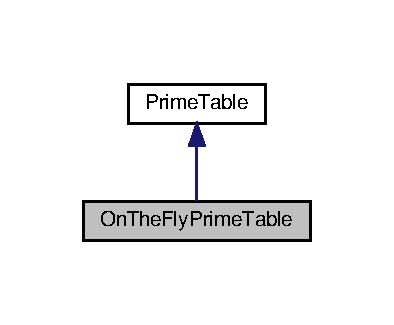
\includegraphics[width=189pt]{classOnTheFlyPrimeTable__inherit__graph}
\end{center}
\end{figure}


Collaboration diagram for On\+The\+Fly\+Prime\+Table\+:\nopagebreak
\begin{figure}[H]
\begin{center}
\leavevmode
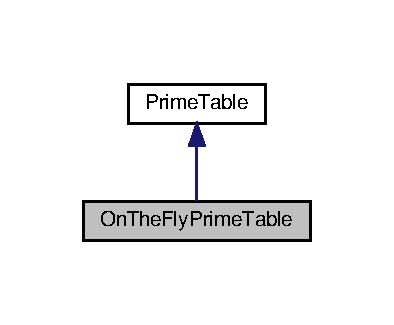
\includegraphics[width=189pt]{classOnTheFlyPrimeTable__coll__graph}
\end{center}
\end{figure}
\subsection*{Public Member Functions}
\begin{DoxyCompactItemize}
\item 
bool \hyperlink{classOnTheFlyPrimeTable_ac8236514299e4558a5220c3e06f7f61a}{Is\+Prime} (int n) const override
\item 
int \hyperlink{classOnTheFlyPrimeTable_a0f6f934f318407a812098e67584b60bf}{Get\+Next\+Prime} (int p) const override
\end{DoxyCompactItemize}


\subsection{Member Function Documentation}
\mbox{\Hypertarget{classOnTheFlyPrimeTable_a0f6f934f318407a812098e67584b60bf}\label{classOnTheFlyPrimeTable_a0f6f934f318407a812098e67584b60bf}} 
\index{On\+The\+Fly\+Prime\+Table@{On\+The\+Fly\+Prime\+Table}!Get\+Next\+Prime@{Get\+Next\+Prime}}
\index{Get\+Next\+Prime@{Get\+Next\+Prime}!On\+The\+Fly\+Prime\+Table@{On\+The\+Fly\+Prime\+Table}}
\subsubsection{\texorpdfstring{Get\+Next\+Prime()}{GetNextPrime()}}
{\footnotesize\ttfamily int On\+The\+Fly\+Prime\+Table\+::\+Get\+Next\+Prime (\begin{DoxyParamCaption}\item[{int}]{p }\end{DoxyParamCaption}) const\hspace{0.3cm}{\ttfamily [inline]}, {\ttfamily [override]}, {\ttfamily [virtual]}}



Implements \hyperlink{classPrimeTable_ae537c939f56617d8937d57bbbae3ab30}{Prime\+Table}.

\mbox{\Hypertarget{classOnTheFlyPrimeTable_ac8236514299e4558a5220c3e06f7f61a}\label{classOnTheFlyPrimeTable_ac8236514299e4558a5220c3e06f7f61a}} 
\index{On\+The\+Fly\+Prime\+Table@{On\+The\+Fly\+Prime\+Table}!Is\+Prime@{Is\+Prime}}
\index{Is\+Prime@{Is\+Prime}!On\+The\+Fly\+Prime\+Table@{On\+The\+Fly\+Prime\+Table}}
\subsubsection{\texorpdfstring{Is\+Prime()}{IsPrime()}}
{\footnotesize\ttfamily bool On\+The\+Fly\+Prime\+Table\+::\+Is\+Prime (\begin{DoxyParamCaption}\item[{int}]{n }\end{DoxyParamCaption}) const\hspace{0.3cm}{\ttfamily [inline]}, {\ttfamily [override]}, {\ttfamily [virtual]}}



Implements \hyperlink{classPrimeTable_a2ab9243364ded0c51541f641b2df362a}{Prime\+Table}.



The documentation for this class was generated from the following file\+:\begin{DoxyCompactItemize}
\item 
tests/googletest/samples/\hyperlink{prime__tables_8h}{prime\+\_\+tables.\+h}\end{DoxyCompactItemize}

\hypertarget{classtesting_1_1internal_1_1ParameterizedTestFactory}{}\section{testing\+:\+:internal\+:\+:Parameterized\+Test\+Factory$<$ Test\+Class $>$ Class Template Reference}
\label{classtesting_1_1internal_1_1ParameterizedTestFactory}\index{testing\+::internal\+::\+Parameterized\+Test\+Factory$<$ Test\+Class $>$@{testing\+::internal\+::\+Parameterized\+Test\+Factory$<$ Test\+Class $>$}}


{\ttfamily \#include $<$gtest-\/param-\/util.\+h$>$}



Inheritance diagram for testing\+:\+:internal\+:\+:Parameterized\+Test\+Factory$<$ Test\+Class $>$\+:\nopagebreak
\begin{figure}[H]
\begin{center}
\leavevmode
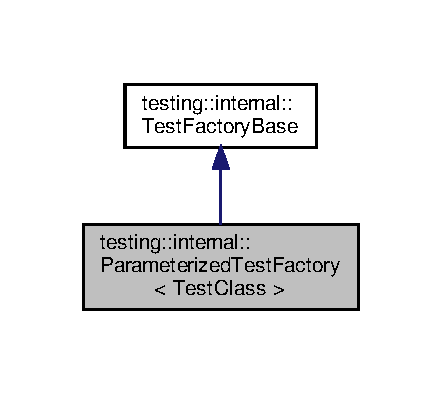
\includegraphics[width=212pt]{classtesting_1_1internal_1_1ParameterizedTestFactory__inherit__graph}
\end{center}
\end{figure}


Collaboration diagram for testing\+:\+:internal\+:\+:Parameterized\+Test\+Factory$<$ Test\+Class $>$\+:\nopagebreak
\begin{figure}[H]
\begin{center}
\leavevmode
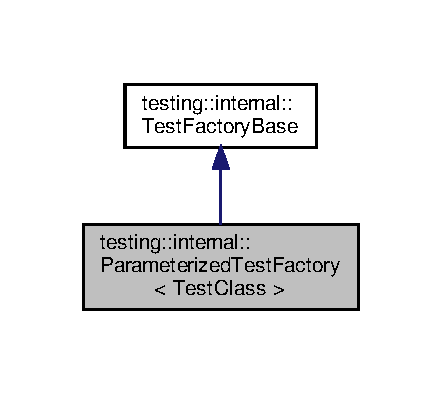
\includegraphics[width=212pt]{classtesting_1_1internal_1_1ParameterizedTestFactory__coll__graph}
\end{center}
\end{figure}
\subsection*{Public Types}
\begin{DoxyCompactItemize}
\item 
typedef Test\+Class\+::\+Param\+Type \hyperlink{classtesting_1_1internal_1_1ParameterizedTestFactory_ad9a27b8e1a83de2f1687625bccff460d}{Param\+Type}
\end{DoxyCompactItemize}
\subsection*{Public Member Functions}
\begin{DoxyCompactItemize}
\item 
\hyperlink{classtesting_1_1internal_1_1ParameterizedTestFactory_a82d78356cd402224255edec760a048fb}{Parameterized\+Test\+Factory} (\hyperlink{classtesting_1_1internal_1_1ParameterizedTestFactory_ad9a27b8e1a83de2f1687625bccff460d}{Param\+Type} parameter)
\item 
\hyperlink{classtesting_1_1Test}{Test} $\ast$ \hyperlink{classtesting_1_1internal_1_1ParameterizedTestFactory_a36d962674d7bf845398637338b9f75cb}{Create\+Test} () override
\end{DoxyCompactItemize}
\subsection*{Private Member Functions}
\begin{DoxyCompactItemize}
\item 
\hyperlink{classtesting_1_1internal_1_1ParameterizedTestFactory_ac70e70bd61d0f66bbc68ed2587c42d92}{G\+T\+E\+S\+T\+\_\+\+D\+I\+S\+A\+L\+L\+O\+W\+\_\+\+C\+O\+P\+Y\+\_\+\+A\+N\+D\+\_\+\+A\+S\+S\+I\+G\+N\+\_\+} (\hyperlink{classtesting_1_1internal_1_1ParameterizedTestFactory}{Parameterized\+Test\+Factory})
\end{DoxyCompactItemize}
\subsection*{Private Attributes}
\begin{DoxyCompactItemize}
\item 
const \hyperlink{classtesting_1_1internal_1_1ParameterizedTestFactory_ad9a27b8e1a83de2f1687625bccff460d}{Param\+Type} \hyperlink{classtesting_1_1internal_1_1ParameterizedTestFactory_a9ee3e72cb3b169924b5328009ed48b5e}{parameter\+\_\+}
\end{DoxyCompactItemize}
\subsection*{Additional Inherited Members}


\subsection{Member Typedef Documentation}
\mbox{\Hypertarget{classtesting_1_1internal_1_1ParameterizedTestFactory_ad9a27b8e1a83de2f1687625bccff460d}\label{classtesting_1_1internal_1_1ParameterizedTestFactory_ad9a27b8e1a83de2f1687625bccff460d}} 
\index{testing\+::internal\+::\+Parameterized\+Test\+Factory@{testing\+::internal\+::\+Parameterized\+Test\+Factory}!Param\+Type@{Param\+Type}}
\index{Param\+Type@{Param\+Type}!testing\+::internal\+::\+Parameterized\+Test\+Factory@{testing\+::internal\+::\+Parameterized\+Test\+Factory}}
\subsubsection{\texorpdfstring{Param\+Type}{ParamType}}
{\footnotesize\ttfamily template$<$class Test\+Class $>$ \\
typedef Test\+Class\+::\+Param\+Type \hyperlink{classtesting_1_1internal_1_1ParameterizedTestFactory}{testing\+::internal\+::\+Parameterized\+Test\+Factory}$<$ Test\+Class $>$\+::\hyperlink{classtesting_1_1internal_1_1ParameterizedTestFactory_ad9a27b8e1a83de2f1687625bccff460d}{Param\+Type}}



\subsection{Constructor \& Destructor Documentation}
\mbox{\Hypertarget{classtesting_1_1internal_1_1ParameterizedTestFactory_a82d78356cd402224255edec760a048fb}\label{classtesting_1_1internal_1_1ParameterizedTestFactory_a82d78356cd402224255edec760a048fb}} 
\index{testing\+::internal\+::\+Parameterized\+Test\+Factory@{testing\+::internal\+::\+Parameterized\+Test\+Factory}!Parameterized\+Test\+Factory@{Parameterized\+Test\+Factory}}
\index{Parameterized\+Test\+Factory@{Parameterized\+Test\+Factory}!testing\+::internal\+::\+Parameterized\+Test\+Factory@{testing\+::internal\+::\+Parameterized\+Test\+Factory}}
\subsubsection{\texorpdfstring{Parameterized\+Test\+Factory()}{ParameterizedTestFactory()}}
{\footnotesize\ttfamily template$<$class Test\+Class $>$ \\
\hyperlink{classtesting_1_1internal_1_1ParameterizedTestFactory}{testing\+::internal\+::\+Parameterized\+Test\+Factory}$<$ Test\+Class $>$\+::\hyperlink{classtesting_1_1internal_1_1ParameterizedTestFactory}{Parameterized\+Test\+Factory} (\begin{DoxyParamCaption}\item[{\hyperlink{classtesting_1_1internal_1_1ParameterizedTestFactory_ad9a27b8e1a83de2f1687625bccff460d}{Param\+Type}}]{parameter }\end{DoxyParamCaption})\hspace{0.3cm}{\ttfamily [inline]}, {\ttfamily [explicit]}}



\subsection{Member Function Documentation}
\mbox{\Hypertarget{classtesting_1_1internal_1_1ParameterizedTestFactory_a36d962674d7bf845398637338b9f75cb}\label{classtesting_1_1internal_1_1ParameterizedTestFactory_a36d962674d7bf845398637338b9f75cb}} 
\index{testing\+::internal\+::\+Parameterized\+Test\+Factory@{testing\+::internal\+::\+Parameterized\+Test\+Factory}!Create\+Test@{Create\+Test}}
\index{Create\+Test@{Create\+Test}!testing\+::internal\+::\+Parameterized\+Test\+Factory@{testing\+::internal\+::\+Parameterized\+Test\+Factory}}
\subsubsection{\texorpdfstring{Create\+Test()}{CreateTest()}}
{\footnotesize\ttfamily template$<$class Test\+Class $>$ \\
\hyperlink{classtesting_1_1Test}{Test}$\ast$ \hyperlink{classtesting_1_1internal_1_1ParameterizedTestFactory}{testing\+::internal\+::\+Parameterized\+Test\+Factory}$<$ Test\+Class $>$\+::Create\+Test (\begin{DoxyParamCaption}{ }\end{DoxyParamCaption})\hspace{0.3cm}{\ttfamily [inline]}, {\ttfamily [override]}, {\ttfamily [virtual]}}



Implements \hyperlink{classtesting_1_1internal_1_1TestFactoryBase_a07ac3ca0b196cdb092da0bb186b7c030}{testing\+::internal\+::\+Test\+Factory\+Base}.

\mbox{\Hypertarget{classtesting_1_1internal_1_1ParameterizedTestFactory_ac70e70bd61d0f66bbc68ed2587c42d92}\label{classtesting_1_1internal_1_1ParameterizedTestFactory_ac70e70bd61d0f66bbc68ed2587c42d92}} 
\index{testing\+::internal\+::\+Parameterized\+Test\+Factory@{testing\+::internal\+::\+Parameterized\+Test\+Factory}!G\+T\+E\+S\+T\+\_\+\+D\+I\+S\+A\+L\+L\+O\+W\+\_\+\+C\+O\+P\+Y\+\_\+\+A\+N\+D\+\_\+\+A\+S\+S\+I\+G\+N\+\_\+@{G\+T\+E\+S\+T\+\_\+\+D\+I\+S\+A\+L\+L\+O\+W\+\_\+\+C\+O\+P\+Y\+\_\+\+A\+N\+D\+\_\+\+A\+S\+S\+I\+G\+N\+\_\+}}
\index{G\+T\+E\+S\+T\+\_\+\+D\+I\+S\+A\+L\+L\+O\+W\+\_\+\+C\+O\+P\+Y\+\_\+\+A\+N\+D\+\_\+\+A\+S\+S\+I\+G\+N\+\_\+@{G\+T\+E\+S\+T\+\_\+\+D\+I\+S\+A\+L\+L\+O\+W\+\_\+\+C\+O\+P\+Y\+\_\+\+A\+N\+D\+\_\+\+A\+S\+S\+I\+G\+N\+\_\+}!testing\+::internal\+::\+Parameterized\+Test\+Factory@{testing\+::internal\+::\+Parameterized\+Test\+Factory}}
\subsubsection{\texorpdfstring{G\+T\+E\+S\+T\+\_\+\+D\+I\+S\+A\+L\+L\+O\+W\+\_\+\+C\+O\+P\+Y\+\_\+\+A\+N\+D\+\_\+\+A\+S\+S\+I\+G\+N\+\_\+()}{GTEST\_DISALLOW\_COPY\_AND\_ASSIGN\_()}}
{\footnotesize\ttfamily template$<$class Test\+Class $>$ \\
\hyperlink{classtesting_1_1internal_1_1ParameterizedTestFactory}{testing\+::internal\+::\+Parameterized\+Test\+Factory}$<$ Test\+Class $>$\+::G\+T\+E\+S\+T\+\_\+\+D\+I\+S\+A\+L\+L\+O\+W\+\_\+\+C\+O\+P\+Y\+\_\+\+A\+N\+D\+\_\+\+A\+S\+S\+I\+G\+N\+\_\+ (\begin{DoxyParamCaption}\item[{\hyperlink{classtesting_1_1internal_1_1ParameterizedTestFactory}{Parameterized\+Test\+Factory}$<$ Test\+Class $>$}]{ }\end{DoxyParamCaption})\hspace{0.3cm}{\ttfamily [private]}}



\subsection{Member Data Documentation}
\mbox{\Hypertarget{classtesting_1_1internal_1_1ParameterizedTestFactory_a9ee3e72cb3b169924b5328009ed48b5e}\label{classtesting_1_1internal_1_1ParameterizedTestFactory_a9ee3e72cb3b169924b5328009ed48b5e}} 
\index{testing\+::internal\+::\+Parameterized\+Test\+Factory@{testing\+::internal\+::\+Parameterized\+Test\+Factory}!parameter\+\_\+@{parameter\+\_\+}}
\index{parameter\+\_\+@{parameter\+\_\+}!testing\+::internal\+::\+Parameterized\+Test\+Factory@{testing\+::internal\+::\+Parameterized\+Test\+Factory}}
\subsubsection{\texorpdfstring{parameter\+\_\+}{parameter\_}}
{\footnotesize\ttfamily template$<$class Test\+Class $>$ \\
const \hyperlink{classtesting_1_1internal_1_1ParameterizedTestFactory_ad9a27b8e1a83de2f1687625bccff460d}{Param\+Type} \hyperlink{classtesting_1_1internal_1_1ParameterizedTestFactory}{testing\+::internal\+::\+Parameterized\+Test\+Factory}$<$ Test\+Class $>$\+::parameter\+\_\+\hspace{0.3cm}{\ttfamily [private]}}



The documentation for this class was generated from the following file\+:\begin{DoxyCompactItemize}
\item 
tests/googletest/include/gtest/internal/\hyperlink{gtest-param-util_8h}{gtest-\/param-\/util.\+h}\end{DoxyCompactItemize}

\hypertarget{classtesting_1_1internal_1_1ParameterizedTestSuiteInfo}{}\section{testing\+:\+:internal\+:\+:Parameterized\+Test\+Suite\+Info$<$ Test\+Suite $>$ Class Template Reference}
\label{classtesting_1_1internal_1_1ParameterizedTestSuiteInfo}\index{testing\+::internal\+::\+Parameterized\+Test\+Suite\+Info$<$ Test\+Suite $>$@{testing\+::internal\+::\+Parameterized\+Test\+Suite\+Info$<$ Test\+Suite $>$}}


{\ttfamily \#include $<$gtest-\/param-\/util.\+h$>$}



Inheritance diagram for testing\+:\+:internal\+:\+:Parameterized\+Test\+Suite\+Info$<$ Test\+Suite $>$\+:\nopagebreak
\begin{figure}[H]
\begin{center}
\leavevmode
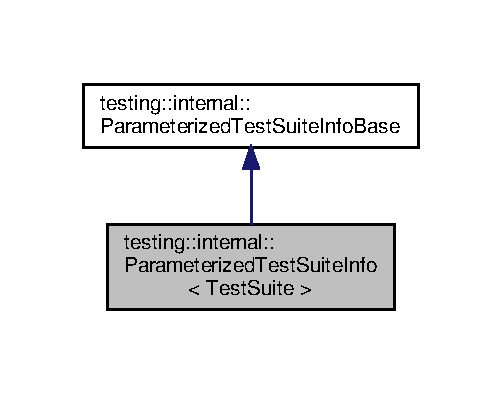
\includegraphics[width=241pt]{classtesting_1_1internal_1_1ParameterizedTestSuiteInfo__inherit__graph}
\end{center}
\end{figure}


Collaboration diagram for testing\+:\+:internal\+:\+:Parameterized\+Test\+Suite\+Info$<$ Test\+Suite $>$\+:\nopagebreak
\begin{figure}[H]
\begin{center}
\leavevmode
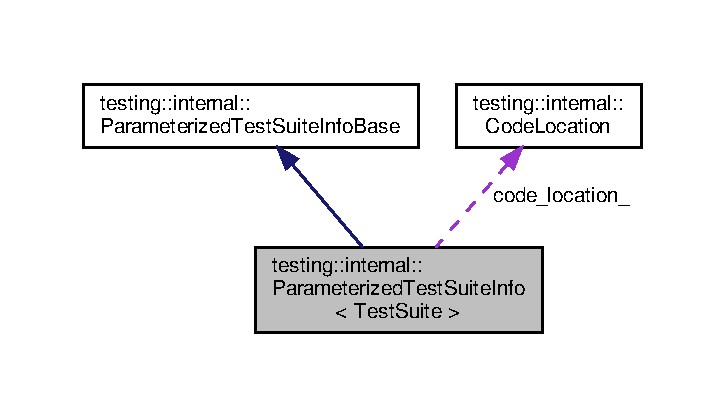
\includegraphics[width=348pt]{classtesting_1_1internal_1_1ParameterizedTestSuiteInfo__coll__graph}
\end{center}
\end{figure}
\subsection*{Classes}
\begin{DoxyCompactItemize}
\item 
struct \hyperlink{structtesting_1_1internal_1_1ParameterizedTestSuiteInfo_1_1InstantiationInfo}{Instantiation\+Info}
\item 
struct \hyperlink{structtesting_1_1internal_1_1ParameterizedTestSuiteInfo_1_1TestInfo}{Test\+Info}
\end{DoxyCompactItemize}
\subsection*{Public Types}
\begin{DoxyCompactItemize}
\item 
using \hyperlink{classtesting_1_1internal_1_1ParameterizedTestSuiteInfo_a10761bd750a6820a8d8d2c654b10fe54}{Param\+Type} = typename Test\+Suite\+::\+Param\+Type
\item 
using \hyperlink{classtesting_1_1internal_1_1ParameterizedTestSuiteInfo_a3b4f232b7d6d3df941bb8e81b6b534a4}{Param\+Name\+Generator\+Func} = std\+::string(const \hyperlink{structtesting_1_1TestParamInfo}{Test\+Param\+Info}$<$ \hyperlink{classtesting_1_1internal_1_1ParameterizedTestSuiteInfo_a10761bd750a6820a8d8d2c654b10fe54}{Param\+Type} $>$ \&)
\end{DoxyCompactItemize}
\subsection*{Public Member Functions}
\begin{DoxyCompactItemize}
\item 
typedef \hyperlink{classtesting_1_1internal_1_1ParameterizedTestSuiteInfo_ac6230057c507d74e373233edbf0410c2}{Param\+Generator} (Generator\+Creation\+Func)()
\item 
\hyperlink{classtesting_1_1internal_1_1ParameterizedTestSuiteInfo_a56fc02ddec2cf2101332d1125e4c75a9}{Parameterized\+Test\+Suite\+Info} (const char $\ast$name, \hyperlink{structtesting_1_1internal_1_1CodeLocation}{Code\+Location} code\+\_\+location)
\item 
const std\+::string \& \hyperlink{classtesting_1_1internal_1_1ParameterizedTestSuiteInfo_a4a5ddc2cd0404438c2b4d405cd0e706c}{Get\+Test\+Suite\+Name} () const override
\item 
\hyperlink{namespacetesting_1_1internal_ab1114197d3c657d8b7f8e0c5caa12d00}{Type\+Id} \hyperlink{classtesting_1_1internal_1_1ParameterizedTestSuiteInfo_af488d1d7c1889a250acff2ea6eba4c84}{Get\+Test\+Suite\+Type\+Id} () const override
\item 
void \hyperlink{classtesting_1_1internal_1_1ParameterizedTestSuiteInfo_a07445ac68713383f38747e1c56c6a04a}{Add\+Test\+Pattern} (const char $\ast$test\+\_\+suite\+\_\+name, const char $\ast$test\+\_\+base\+\_\+name, \hyperlink{classtesting_1_1internal_1_1TestMetaFactoryBase}{Test\+Meta\+Factory\+Base}$<$ \hyperlink{classtesting_1_1internal_1_1ParameterizedTestSuiteInfo_a10761bd750a6820a8d8d2c654b10fe54}{Param\+Type} $>$ $\ast$meta\+\_\+factory)
\item 
int \hyperlink{classtesting_1_1internal_1_1ParameterizedTestSuiteInfo_a174f164f38e522a3935da911a9c1e450}{Add\+Test\+Suite\+Instantiation} (const std\+::string \&instantiation\+\_\+name, Generator\+Creation\+Func $\ast$func, \hyperlink{classtesting_1_1internal_1_1ParameterizedTestSuiteInfo_a3b4f232b7d6d3df941bb8e81b6b534a4}{Param\+Name\+Generator\+Func} $\ast$name\+\_\+func, const char $\ast$file, int line)
\item 
void \hyperlink{classtesting_1_1internal_1_1ParameterizedTestSuiteInfo_a8c0af866d3c291a63d3f4581ccd452d1}{Register\+Tests} () override
\end{DoxyCompactItemize}
\subsection*{Private Types}
\begin{DoxyCompactItemize}
\item 
using \hyperlink{classtesting_1_1internal_1_1ParameterizedTestSuiteInfo_a0578de1b5b1852655771349b785d7fb7}{Test\+Info\+Container} = \+::std\+::vector$<$ std\+::shared\+\_\+ptr$<$ \hyperlink{structtesting_1_1internal_1_1ParameterizedTestSuiteInfo_1_1TestInfo}{Test\+Info} $>$ $>$
\item 
typedef \+::std\+::vector$<$ \hyperlink{structtesting_1_1internal_1_1ParameterizedTestSuiteInfo_1_1InstantiationInfo}{Instantiation\+Info} $>$ \hyperlink{classtesting_1_1internal_1_1ParameterizedTestSuiteInfo_a65cee35a4b9653272b6017640816eb68}{Instantiation\+Container}
\end{DoxyCompactItemize}
\subsection*{Private Member Functions}
\begin{DoxyCompactItemize}
\item 
\hyperlink{classtesting_1_1internal_1_1ParameterizedTestSuiteInfo_a2370bc6f72b85b499fa05c375358df9e}{G\+T\+E\+S\+T\+\_\+\+D\+I\+S\+A\+L\+L\+O\+W\+\_\+\+C\+O\+P\+Y\+\_\+\+A\+N\+D\+\_\+\+A\+S\+S\+I\+G\+N\+\_\+} (\hyperlink{classtesting_1_1internal_1_1ParameterizedTestSuiteInfo}{Parameterized\+Test\+Suite\+Info})
\end{DoxyCompactItemize}
\subsection*{Static Private Member Functions}
\begin{DoxyCompactItemize}
\item 
static bool \hyperlink{classtesting_1_1internal_1_1ParameterizedTestSuiteInfo_a978b6780b449fc1ad63dec758e899679}{Is\+Valid\+Param\+Name} (const std\+::string \&name)
\end{DoxyCompactItemize}
\subsection*{Private Attributes}
\begin{DoxyCompactItemize}
\item 
const std\+::string \hyperlink{classtesting_1_1internal_1_1ParameterizedTestSuiteInfo_a59effa7c65294abcc39772281f97f13f}{test\+\_\+suite\+\_\+name\+\_\+}
\item 
\hyperlink{structtesting_1_1internal_1_1CodeLocation}{Code\+Location} \hyperlink{classtesting_1_1internal_1_1ParameterizedTestSuiteInfo_a64949444440296996cd9ee66e270a459}{code\+\_\+location\+\_\+}
\item 
\hyperlink{classtesting_1_1internal_1_1ParameterizedTestSuiteInfo_a0578de1b5b1852655771349b785d7fb7}{Test\+Info\+Container} \hyperlink{classtesting_1_1internal_1_1ParameterizedTestSuiteInfo_a44e991246e79e6587ffd35533ab4e2d3}{tests\+\_\+}
\item 
\hyperlink{classtesting_1_1internal_1_1ParameterizedTestSuiteInfo_a65cee35a4b9653272b6017640816eb68}{Instantiation\+Container} \hyperlink{classtesting_1_1internal_1_1ParameterizedTestSuiteInfo_a7334ea96f0aab82af68c36e3c62c49ab}{instantiations\+\_\+}
\end{DoxyCompactItemize}
\subsection*{Additional Inherited Members}


\subsection{Member Typedef Documentation}
\mbox{\Hypertarget{classtesting_1_1internal_1_1ParameterizedTestSuiteInfo_a65cee35a4b9653272b6017640816eb68}\label{classtesting_1_1internal_1_1ParameterizedTestSuiteInfo_a65cee35a4b9653272b6017640816eb68}} 
\index{testing\+::internal\+::\+Parameterized\+Test\+Suite\+Info@{testing\+::internal\+::\+Parameterized\+Test\+Suite\+Info}!Instantiation\+Container@{Instantiation\+Container}}
\index{Instantiation\+Container@{Instantiation\+Container}!testing\+::internal\+::\+Parameterized\+Test\+Suite\+Info@{testing\+::internal\+::\+Parameterized\+Test\+Suite\+Info}}
\subsubsection{\texorpdfstring{Instantiation\+Container}{InstantiationContainer}}
{\footnotesize\ttfamily template$<$class Test\+Suite$>$ \\
typedef \+::std\+::vector$<$\hyperlink{structtesting_1_1internal_1_1ParameterizedTestSuiteInfo_1_1InstantiationInfo}{Instantiation\+Info}$>$ \hyperlink{classtesting_1_1internal_1_1ParameterizedTestSuiteInfo}{testing\+::internal\+::\+Parameterized\+Test\+Suite\+Info}$<$ \hyperlink{classtesting_1_1TestSuite}{Test\+Suite} $>$\+::\hyperlink{classtesting_1_1internal_1_1ParameterizedTestSuiteInfo_a65cee35a4b9653272b6017640816eb68}{Instantiation\+Container}\hspace{0.3cm}{\ttfamily [private]}}

\mbox{\Hypertarget{classtesting_1_1internal_1_1ParameterizedTestSuiteInfo_a3b4f232b7d6d3df941bb8e81b6b534a4}\label{classtesting_1_1internal_1_1ParameterizedTestSuiteInfo_a3b4f232b7d6d3df941bb8e81b6b534a4}} 
\index{testing\+::internal\+::\+Parameterized\+Test\+Suite\+Info@{testing\+::internal\+::\+Parameterized\+Test\+Suite\+Info}!Param\+Name\+Generator\+Func@{Param\+Name\+Generator\+Func}}
\index{Param\+Name\+Generator\+Func@{Param\+Name\+Generator\+Func}!testing\+::internal\+::\+Parameterized\+Test\+Suite\+Info@{testing\+::internal\+::\+Parameterized\+Test\+Suite\+Info}}
\subsubsection{\texorpdfstring{Param\+Name\+Generator\+Func}{ParamNameGeneratorFunc}}
{\footnotesize\ttfamily template$<$class Test\+Suite$>$ \\
using \hyperlink{classtesting_1_1internal_1_1ParameterizedTestSuiteInfo}{testing\+::internal\+::\+Parameterized\+Test\+Suite\+Info}$<$ \hyperlink{classtesting_1_1TestSuite}{Test\+Suite} $>$\+::\hyperlink{classtesting_1_1internal_1_1ParameterizedTestSuiteInfo_a3b4f232b7d6d3df941bb8e81b6b534a4}{Param\+Name\+Generator\+Func} =  std\+::string(const \hyperlink{structtesting_1_1TestParamInfo}{Test\+Param\+Info}$<$\hyperlink{classtesting_1_1internal_1_1ParameterizedTestSuiteInfo_a10761bd750a6820a8d8d2c654b10fe54}{Param\+Type}$>$\&)}

\mbox{\Hypertarget{classtesting_1_1internal_1_1ParameterizedTestSuiteInfo_a10761bd750a6820a8d8d2c654b10fe54}\label{classtesting_1_1internal_1_1ParameterizedTestSuiteInfo_a10761bd750a6820a8d8d2c654b10fe54}} 
\index{testing\+::internal\+::\+Parameterized\+Test\+Suite\+Info@{testing\+::internal\+::\+Parameterized\+Test\+Suite\+Info}!Param\+Type@{Param\+Type}}
\index{Param\+Type@{Param\+Type}!testing\+::internal\+::\+Parameterized\+Test\+Suite\+Info@{testing\+::internal\+::\+Parameterized\+Test\+Suite\+Info}}
\subsubsection{\texorpdfstring{Param\+Type}{ParamType}}
{\footnotesize\ttfamily template$<$class Test\+Suite$>$ \\
using \hyperlink{classtesting_1_1internal_1_1ParameterizedTestSuiteInfo}{testing\+::internal\+::\+Parameterized\+Test\+Suite\+Info}$<$ \hyperlink{classtesting_1_1TestSuite}{Test\+Suite} $>$\+::\hyperlink{classtesting_1_1internal_1_1ParameterizedTestSuiteInfo_a10761bd750a6820a8d8d2c654b10fe54}{Param\+Type} =  typename Test\+Suite\+::\+Param\+Type}

\mbox{\Hypertarget{classtesting_1_1internal_1_1ParameterizedTestSuiteInfo_a0578de1b5b1852655771349b785d7fb7}\label{classtesting_1_1internal_1_1ParameterizedTestSuiteInfo_a0578de1b5b1852655771349b785d7fb7}} 
\index{testing\+::internal\+::\+Parameterized\+Test\+Suite\+Info@{testing\+::internal\+::\+Parameterized\+Test\+Suite\+Info}!Test\+Info\+Container@{Test\+Info\+Container}}
\index{Test\+Info\+Container@{Test\+Info\+Container}!testing\+::internal\+::\+Parameterized\+Test\+Suite\+Info@{testing\+::internal\+::\+Parameterized\+Test\+Suite\+Info}}
\subsubsection{\texorpdfstring{Test\+Info\+Container}{TestInfoContainer}}
{\footnotesize\ttfamily template$<$class Test\+Suite$>$ \\
using \hyperlink{classtesting_1_1internal_1_1ParameterizedTestSuiteInfo}{testing\+::internal\+::\+Parameterized\+Test\+Suite\+Info}$<$ \hyperlink{classtesting_1_1TestSuite}{Test\+Suite} $>$\+::\hyperlink{classtesting_1_1internal_1_1ParameterizedTestSuiteInfo_a0578de1b5b1852655771349b785d7fb7}{Test\+Info\+Container} =  \+::std\+::vector$<$std\+::shared\+\_\+ptr$<$\hyperlink{structtesting_1_1internal_1_1ParameterizedTestSuiteInfo_1_1TestInfo}{Test\+Info}$>$ $>$\hspace{0.3cm}{\ttfamily [private]}}



\subsection{Constructor \& Destructor Documentation}
\mbox{\Hypertarget{classtesting_1_1internal_1_1ParameterizedTestSuiteInfo_a56fc02ddec2cf2101332d1125e4c75a9}\label{classtesting_1_1internal_1_1ParameterizedTestSuiteInfo_a56fc02ddec2cf2101332d1125e4c75a9}} 
\index{testing\+::internal\+::\+Parameterized\+Test\+Suite\+Info@{testing\+::internal\+::\+Parameterized\+Test\+Suite\+Info}!Parameterized\+Test\+Suite\+Info@{Parameterized\+Test\+Suite\+Info}}
\index{Parameterized\+Test\+Suite\+Info@{Parameterized\+Test\+Suite\+Info}!testing\+::internal\+::\+Parameterized\+Test\+Suite\+Info@{testing\+::internal\+::\+Parameterized\+Test\+Suite\+Info}}
\subsubsection{\texorpdfstring{Parameterized\+Test\+Suite\+Info()}{ParameterizedTestSuiteInfo()}}
{\footnotesize\ttfamily template$<$class Test\+Suite$>$ \\
\hyperlink{classtesting_1_1internal_1_1ParameterizedTestSuiteInfo}{testing\+::internal\+::\+Parameterized\+Test\+Suite\+Info}$<$ \hyperlink{classtesting_1_1TestSuite}{Test\+Suite} $>$\+::\hyperlink{classtesting_1_1internal_1_1ParameterizedTestSuiteInfo}{Parameterized\+Test\+Suite\+Info} (\begin{DoxyParamCaption}\item[{const char $\ast$}]{name,  }\item[{\hyperlink{structtesting_1_1internal_1_1CodeLocation}{Code\+Location}}]{code\+\_\+location }\end{DoxyParamCaption})\hspace{0.3cm}{\ttfamily [inline]}, {\ttfamily [explicit]}}



\subsection{Member Function Documentation}
\mbox{\Hypertarget{classtesting_1_1internal_1_1ParameterizedTestSuiteInfo_a07445ac68713383f38747e1c56c6a04a}\label{classtesting_1_1internal_1_1ParameterizedTestSuiteInfo_a07445ac68713383f38747e1c56c6a04a}} 
\index{testing\+::internal\+::\+Parameterized\+Test\+Suite\+Info@{testing\+::internal\+::\+Parameterized\+Test\+Suite\+Info}!Add\+Test\+Pattern@{Add\+Test\+Pattern}}
\index{Add\+Test\+Pattern@{Add\+Test\+Pattern}!testing\+::internal\+::\+Parameterized\+Test\+Suite\+Info@{testing\+::internal\+::\+Parameterized\+Test\+Suite\+Info}}
\subsubsection{\texorpdfstring{Add\+Test\+Pattern()}{AddTestPattern()}}
{\footnotesize\ttfamily template$<$class Test\+Suite$>$ \\
void \hyperlink{classtesting_1_1internal_1_1ParameterizedTestSuiteInfo}{testing\+::internal\+::\+Parameterized\+Test\+Suite\+Info}$<$ \hyperlink{classtesting_1_1TestSuite}{Test\+Suite} $>$\+::Add\+Test\+Pattern (\begin{DoxyParamCaption}\item[{const char $\ast$}]{test\+\_\+suite\+\_\+name,  }\item[{const char $\ast$}]{test\+\_\+base\+\_\+name,  }\item[{\hyperlink{classtesting_1_1internal_1_1TestMetaFactoryBase}{Test\+Meta\+Factory\+Base}$<$ \hyperlink{classtesting_1_1internal_1_1ParameterizedTestSuiteInfo_a10761bd750a6820a8d8d2c654b10fe54}{Param\+Type} $>$ $\ast$}]{meta\+\_\+factory }\end{DoxyParamCaption})\hspace{0.3cm}{\ttfamily [inline]}}

\mbox{\Hypertarget{classtesting_1_1internal_1_1ParameterizedTestSuiteInfo_a174f164f38e522a3935da911a9c1e450}\label{classtesting_1_1internal_1_1ParameterizedTestSuiteInfo_a174f164f38e522a3935da911a9c1e450}} 
\index{testing\+::internal\+::\+Parameterized\+Test\+Suite\+Info@{testing\+::internal\+::\+Parameterized\+Test\+Suite\+Info}!Add\+Test\+Suite\+Instantiation@{Add\+Test\+Suite\+Instantiation}}
\index{Add\+Test\+Suite\+Instantiation@{Add\+Test\+Suite\+Instantiation}!testing\+::internal\+::\+Parameterized\+Test\+Suite\+Info@{testing\+::internal\+::\+Parameterized\+Test\+Suite\+Info}}
\subsubsection{\texorpdfstring{Add\+Test\+Suite\+Instantiation()}{AddTestSuiteInstantiation()}}
{\footnotesize\ttfamily template$<$class Test\+Suite$>$ \\
int \hyperlink{classtesting_1_1internal_1_1ParameterizedTestSuiteInfo}{testing\+::internal\+::\+Parameterized\+Test\+Suite\+Info}$<$ \hyperlink{classtesting_1_1TestSuite}{Test\+Suite} $>$\+::Add\+Test\+Suite\+Instantiation (\begin{DoxyParamCaption}\item[{const std\+::string \&}]{instantiation\+\_\+name,  }\item[{Generator\+Creation\+Func $\ast$}]{func,  }\item[{\hyperlink{classtesting_1_1internal_1_1ParameterizedTestSuiteInfo_a3b4f232b7d6d3df941bb8e81b6b534a4}{Param\+Name\+Generator\+Func} $\ast$}]{name\+\_\+func,  }\item[{const char $\ast$}]{file,  }\item[{int}]{line }\end{DoxyParamCaption})\hspace{0.3cm}{\ttfamily [inline]}}

\mbox{\Hypertarget{classtesting_1_1internal_1_1ParameterizedTestSuiteInfo_a4a5ddc2cd0404438c2b4d405cd0e706c}\label{classtesting_1_1internal_1_1ParameterizedTestSuiteInfo_a4a5ddc2cd0404438c2b4d405cd0e706c}} 
\index{testing\+::internal\+::\+Parameterized\+Test\+Suite\+Info@{testing\+::internal\+::\+Parameterized\+Test\+Suite\+Info}!Get\+Test\+Suite\+Name@{Get\+Test\+Suite\+Name}}
\index{Get\+Test\+Suite\+Name@{Get\+Test\+Suite\+Name}!testing\+::internal\+::\+Parameterized\+Test\+Suite\+Info@{testing\+::internal\+::\+Parameterized\+Test\+Suite\+Info}}
\subsubsection{\texorpdfstring{Get\+Test\+Suite\+Name()}{GetTestSuiteName()}}
{\footnotesize\ttfamily template$<$class Test\+Suite$>$ \\
const std\+::string\& \hyperlink{classtesting_1_1internal_1_1ParameterizedTestSuiteInfo}{testing\+::internal\+::\+Parameterized\+Test\+Suite\+Info}$<$ \hyperlink{classtesting_1_1TestSuite}{Test\+Suite} $>$\+::Get\+Test\+Suite\+Name (\begin{DoxyParamCaption}{ }\end{DoxyParamCaption}) const\hspace{0.3cm}{\ttfamily [inline]}, {\ttfamily [override]}, {\ttfamily [virtual]}}



Implements \hyperlink{classtesting_1_1internal_1_1ParameterizedTestSuiteInfoBase_aa6e36241431dc72c251ecee9b637b4d3}{testing\+::internal\+::\+Parameterized\+Test\+Suite\+Info\+Base}.

\mbox{\Hypertarget{classtesting_1_1internal_1_1ParameterizedTestSuiteInfo_af488d1d7c1889a250acff2ea6eba4c84}\label{classtesting_1_1internal_1_1ParameterizedTestSuiteInfo_af488d1d7c1889a250acff2ea6eba4c84}} 
\index{testing\+::internal\+::\+Parameterized\+Test\+Suite\+Info@{testing\+::internal\+::\+Parameterized\+Test\+Suite\+Info}!Get\+Test\+Suite\+Type\+Id@{Get\+Test\+Suite\+Type\+Id}}
\index{Get\+Test\+Suite\+Type\+Id@{Get\+Test\+Suite\+Type\+Id}!testing\+::internal\+::\+Parameterized\+Test\+Suite\+Info@{testing\+::internal\+::\+Parameterized\+Test\+Suite\+Info}}
\subsubsection{\texorpdfstring{Get\+Test\+Suite\+Type\+Id()}{GetTestSuiteTypeId()}}
{\footnotesize\ttfamily template$<$class Test\+Suite$>$ \\
\hyperlink{namespacetesting_1_1internal_ab1114197d3c657d8b7f8e0c5caa12d00}{Type\+Id} \hyperlink{classtesting_1_1internal_1_1ParameterizedTestSuiteInfo}{testing\+::internal\+::\+Parameterized\+Test\+Suite\+Info}$<$ \hyperlink{classtesting_1_1TestSuite}{Test\+Suite} $>$\+::Get\+Test\+Suite\+Type\+Id (\begin{DoxyParamCaption}{ }\end{DoxyParamCaption}) const\hspace{0.3cm}{\ttfamily [inline]}, {\ttfamily [override]}, {\ttfamily [virtual]}}



Implements \hyperlink{classtesting_1_1internal_1_1ParameterizedTestSuiteInfoBase_ac5bcbf8c50a44472d697e0c80b54387d}{testing\+::internal\+::\+Parameterized\+Test\+Suite\+Info\+Base}.

\mbox{\Hypertarget{classtesting_1_1internal_1_1ParameterizedTestSuiteInfo_a2370bc6f72b85b499fa05c375358df9e}\label{classtesting_1_1internal_1_1ParameterizedTestSuiteInfo_a2370bc6f72b85b499fa05c375358df9e}} 
\index{testing\+::internal\+::\+Parameterized\+Test\+Suite\+Info@{testing\+::internal\+::\+Parameterized\+Test\+Suite\+Info}!G\+T\+E\+S\+T\+\_\+\+D\+I\+S\+A\+L\+L\+O\+W\+\_\+\+C\+O\+P\+Y\+\_\+\+A\+N\+D\+\_\+\+A\+S\+S\+I\+G\+N\+\_\+@{G\+T\+E\+S\+T\+\_\+\+D\+I\+S\+A\+L\+L\+O\+W\+\_\+\+C\+O\+P\+Y\+\_\+\+A\+N\+D\+\_\+\+A\+S\+S\+I\+G\+N\+\_\+}}
\index{G\+T\+E\+S\+T\+\_\+\+D\+I\+S\+A\+L\+L\+O\+W\+\_\+\+C\+O\+P\+Y\+\_\+\+A\+N\+D\+\_\+\+A\+S\+S\+I\+G\+N\+\_\+@{G\+T\+E\+S\+T\+\_\+\+D\+I\+S\+A\+L\+L\+O\+W\+\_\+\+C\+O\+P\+Y\+\_\+\+A\+N\+D\+\_\+\+A\+S\+S\+I\+G\+N\+\_\+}!testing\+::internal\+::\+Parameterized\+Test\+Suite\+Info@{testing\+::internal\+::\+Parameterized\+Test\+Suite\+Info}}
\subsubsection{\texorpdfstring{G\+T\+E\+S\+T\+\_\+\+D\+I\+S\+A\+L\+L\+O\+W\+\_\+\+C\+O\+P\+Y\+\_\+\+A\+N\+D\+\_\+\+A\+S\+S\+I\+G\+N\+\_\+()}{GTEST\_DISALLOW\_COPY\_AND\_ASSIGN\_()}}
{\footnotesize\ttfamily template$<$class Test\+Suite$>$ \\
\hyperlink{classtesting_1_1internal_1_1ParameterizedTestSuiteInfo}{testing\+::internal\+::\+Parameterized\+Test\+Suite\+Info}$<$ \hyperlink{classtesting_1_1TestSuite}{Test\+Suite} $>$\+::G\+T\+E\+S\+T\+\_\+\+D\+I\+S\+A\+L\+L\+O\+W\+\_\+\+C\+O\+P\+Y\+\_\+\+A\+N\+D\+\_\+\+A\+S\+S\+I\+G\+N\+\_\+ (\begin{DoxyParamCaption}\item[{\hyperlink{classtesting_1_1internal_1_1ParameterizedTestSuiteInfo}{Parameterized\+Test\+Suite\+Info}$<$ \hyperlink{classtesting_1_1TestSuite}{Test\+Suite} $>$}]{ }\end{DoxyParamCaption})\hspace{0.3cm}{\ttfamily [private]}}

\mbox{\Hypertarget{classtesting_1_1internal_1_1ParameterizedTestSuiteInfo_a978b6780b449fc1ad63dec758e899679}\label{classtesting_1_1internal_1_1ParameterizedTestSuiteInfo_a978b6780b449fc1ad63dec758e899679}} 
\index{testing\+::internal\+::\+Parameterized\+Test\+Suite\+Info@{testing\+::internal\+::\+Parameterized\+Test\+Suite\+Info}!Is\+Valid\+Param\+Name@{Is\+Valid\+Param\+Name}}
\index{Is\+Valid\+Param\+Name@{Is\+Valid\+Param\+Name}!testing\+::internal\+::\+Parameterized\+Test\+Suite\+Info@{testing\+::internal\+::\+Parameterized\+Test\+Suite\+Info}}
\subsubsection{\texorpdfstring{Is\+Valid\+Param\+Name()}{IsValidParamName()}}
{\footnotesize\ttfamily template$<$class Test\+Suite$>$ \\
static bool \hyperlink{classtesting_1_1internal_1_1ParameterizedTestSuiteInfo}{testing\+::internal\+::\+Parameterized\+Test\+Suite\+Info}$<$ \hyperlink{classtesting_1_1TestSuite}{Test\+Suite} $>$\+::Is\+Valid\+Param\+Name (\begin{DoxyParamCaption}\item[{const std\+::string \&}]{name }\end{DoxyParamCaption})\hspace{0.3cm}{\ttfamily [inline]}, {\ttfamily [static]}, {\ttfamily [private]}}

\mbox{\Hypertarget{classtesting_1_1internal_1_1ParameterizedTestSuiteInfo_ac6230057c507d74e373233edbf0410c2}\label{classtesting_1_1internal_1_1ParameterizedTestSuiteInfo_ac6230057c507d74e373233edbf0410c2}} 
\index{testing\+::internal\+::\+Parameterized\+Test\+Suite\+Info@{testing\+::internal\+::\+Parameterized\+Test\+Suite\+Info}!Param\+Generator@{Param\+Generator}}
\index{Param\+Generator@{Param\+Generator}!testing\+::internal\+::\+Parameterized\+Test\+Suite\+Info@{testing\+::internal\+::\+Parameterized\+Test\+Suite\+Info}}
\subsubsection{\texorpdfstring{Param\+Generator()}{ParamGenerator()}}
{\footnotesize\ttfamily template$<$class Test\+Suite$>$ \\
typedef \hyperlink{classtesting_1_1internal_1_1ParameterizedTestSuiteInfo}{testing\+::internal\+::\+Parameterized\+Test\+Suite\+Info}$<$ \hyperlink{classtesting_1_1TestSuite}{Test\+Suite} $>$\+::\hyperlink{classtesting_1_1internal_1_1ParamGenerator}{Param\+Generator} (\begin{DoxyParamCaption}\item[{Generator\+Creation\+Func}]{ }\end{DoxyParamCaption})}

\mbox{\Hypertarget{classtesting_1_1internal_1_1ParameterizedTestSuiteInfo_a8c0af866d3c291a63d3f4581ccd452d1}\label{classtesting_1_1internal_1_1ParameterizedTestSuiteInfo_a8c0af866d3c291a63d3f4581ccd452d1}} 
\index{testing\+::internal\+::\+Parameterized\+Test\+Suite\+Info@{testing\+::internal\+::\+Parameterized\+Test\+Suite\+Info}!Register\+Tests@{Register\+Tests}}
\index{Register\+Tests@{Register\+Tests}!testing\+::internal\+::\+Parameterized\+Test\+Suite\+Info@{testing\+::internal\+::\+Parameterized\+Test\+Suite\+Info}}
\subsubsection{\texorpdfstring{Register\+Tests()}{RegisterTests()}}
{\footnotesize\ttfamily template$<$class Test\+Suite$>$ \\
void \hyperlink{classtesting_1_1internal_1_1ParameterizedTestSuiteInfo}{testing\+::internal\+::\+Parameterized\+Test\+Suite\+Info}$<$ \hyperlink{classtesting_1_1TestSuite}{Test\+Suite} $>$\+::Register\+Tests (\begin{DoxyParamCaption}{ }\end{DoxyParamCaption})\hspace{0.3cm}{\ttfamily [inline]}, {\ttfamily [override]}, {\ttfamily [virtual]}}



Implements \hyperlink{classtesting_1_1internal_1_1ParameterizedTestSuiteInfoBase_a41d7d663014af0c1e614c5a61293cb5a}{testing\+::internal\+::\+Parameterized\+Test\+Suite\+Info\+Base}.



\subsection{Member Data Documentation}
\mbox{\Hypertarget{classtesting_1_1internal_1_1ParameterizedTestSuiteInfo_a64949444440296996cd9ee66e270a459}\label{classtesting_1_1internal_1_1ParameterizedTestSuiteInfo_a64949444440296996cd9ee66e270a459}} 
\index{testing\+::internal\+::\+Parameterized\+Test\+Suite\+Info@{testing\+::internal\+::\+Parameterized\+Test\+Suite\+Info}!code\+\_\+location\+\_\+@{code\+\_\+location\+\_\+}}
\index{code\+\_\+location\+\_\+@{code\+\_\+location\+\_\+}!testing\+::internal\+::\+Parameterized\+Test\+Suite\+Info@{testing\+::internal\+::\+Parameterized\+Test\+Suite\+Info}}
\subsubsection{\texorpdfstring{code\+\_\+location\+\_\+}{code\_location\_}}
{\footnotesize\ttfamily template$<$class Test\+Suite$>$ \\
\hyperlink{structtesting_1_1internal_1_1CodeLocation}{Code\+Location} \hyperlink{classtesting_1_1internal_1_1ParameterizedTestSuiteInfo}{testing\+::internal\+::\+Parameterized\+Test\+Suite\+Info}$<$ \hyperlink{classtesting_1_1TestSuite}{Test\+Suite} $>$\+::code\+\_\+location\+\_\+\hspace{0.3cm}{\ttfamily [private]}}

\mbox{\Hypertarget{classtesting_1_1internal_1_1ParameterizedTestSuiteInfo_a7334ea96f0aab82af68c36e3c62c49ab}\label{classtesting_1_1internal_1_1ParameterizedTestSuiteInfo_a7334ea96f0aab82af68c36e3c62c49ab}} 
\index{testing\+::internal\+::\+Parameterized\+Test\+Suite\+Info@{testing\+::internal\+::\+Parameterized\+Test\+Suite\+Info}!instantiations\+\_\+@{instantiations\+\_\+}}
\index{instantiations\+\_\+@{instantiations\+\_\+}!testing\+::internal\+::\+Parameterized\+Test\+Suite\+Info@{testing\+::internal\+::\+Parameterized\+Test\+Suite\+Info}}
\subsubsection{\texorpdfstring{instantiations\+\_\+}{instantiations\_}}
{\footnotesize\ttfamily template$<$class Test\+Suite$>$ \\
\hyperlink{classtesting_1_1internal_1_1ParameterizedTestSuiteInfo_a65cee35a4b9653272b6017640816eb68}{Instantiation\+Container} \hyperlink{classtesting_1_1internal_1_1ParameterizedTestSuiteInfo}{testing\+::internal\+::\+Parameterized\+Test\+Suite\+Info}$<$ \hyperlink{classtesting_1_1TestSuite}{Test\+Suite} $>$\+::instantiations\+\_\+\hspace{0.3cm}{\ttfamily [private]}}

\mbox{\Hypertarget{classtesting_1_1internal_1_1ParameterizedTestSuiteInfo_a59effa7c65294abcc39772281f97f13f}\label{classtesting_1_1internal_1_1ParameterizedTestSuiteInfo_a59effa7c65294abcc39772281f97f13f}} 
\index{testing\+::internal\+::\+Parameterized\+Test\+Suite\+Info@{testing\+::internal\+::\+Parameterized\+Test\+Suite\+Info}!test\+\_\+suite\+\_\+name\+\_\+@{test\+\_\+suite\+\_\+name\+\_\+}}
\index{test\+\_\+suite\+\_\+name\+\_\+@{test\+\_\+suite\+\_\+name\+\_\+}!testing\+::internal\+::\+Parameterized\+Test\+Suite\+Info@{testing\+::internal\+::\+Parameterized\+Test\+Suite\+Info}}
\subsubsection{\texorpdfstring{test\+\_\+suite\+\_\+name\+\_\+}{test\_suite\_name\_}}
{\footnotesize\ttfamily template$<$class Test\+Suite$>$ \\
const std\+::string \hyperlink{classtesting_1_1internal_1_1ParameterizedTestSuiteInfo}{testing\+::internal\+::\+Parameterized\+Test\+Suite\+Info}$<$ \hyperlink{classtesting_1_1TestSuite}{Test\+Suite} $>$\+::test\+\_\+suite\+\_\+name\+\_\+\hspace{0.3cm}{\ttfamily [private]}}

\mbox{\Hypertarget{classtesting_1_1internal_1_1ParameterizedTestSuiteInfo_a44e991246e79e6587ffd35533ab4e2d3}\label{classtesting_1_1internal_1_1ParameterizedTestSuiteInfo_a44e991246e79e6587ffd35533ab4e2d3}} 
\index{testing\+::internal\+::\+Parameterized\+Test\+Suite\+Info@{testing\+::internal\+::\+Parameterized\+Test\+Suite\+Info}!tests\+\_\+@{tests\+\_\+}}
\index{tests\+\_\+@{tests\+\_\+}!testing\+::internal\+::\+Parameterized\+Test\+Suite\+Info@{testing\+::internal\+::\+Parameterized\+Test\+Suite\+Info}}
\subsubsection{\texorpdfstring{tests\+\_\+}{tests\_}}
{\footnotesize\ttfamily template$<$class Test\+Suite$>$ \\
\hyperlink{classtesting_1_1internal_1_1ParameterizedTestSuiteInfo_a0578de1b5b1852655771349b785d7fb7}{Test\+Info\+Container} \hyperlink{classtesting_1_1internal_1_1ParameterizedTestSuiteInfo}{testing\+::internal\+::\+Parameterized\+Test\+Suite\+Info}$<$ \hyperlink{classtesting_1_1TestSuite}{Test\+Suite} $>$\+::tests\+\_\+\hspace{0.3cm}{\ttfamily [private]}}



The documentation for this class was generated from the following file\+:\begin{DoxyCompactItemize}
\item 
tests/googletest/include/gtest/internal/\hyperlink{gtest-param-util_8h}{gtest-\/param-\/util.\+h}\end{DoxyCompactItemize}

\hypertarget{classtesting_1_1internal_1_1ParameterizedTestSuiteInfoBase}{}\section{testing\+:\+:internal\+:\+:Parameterized\+Test\+Suite\+Info\+Base Class Reference}
\label{classtesting_1_1internal_1_1ParameterizedTestSuiteInfoBase}\index{testing\+::internal\+::\+Parameterized\+Test\+Suite\+Info\+Base@{testing\+::internal\+::\+Parameterized\+Test\+Suite\+Info\+Base}}


{\ttfamily \#include $<$gtest-\/param-\/util.\+h$>$}



Inheritance diagram for testing\+:\+:internal\+:\+:Parameterized\+Test\+Suite\+Info\+Base\+:\nopagebreak
\begin{figure}[H]
\begin{center}
\leavevmode
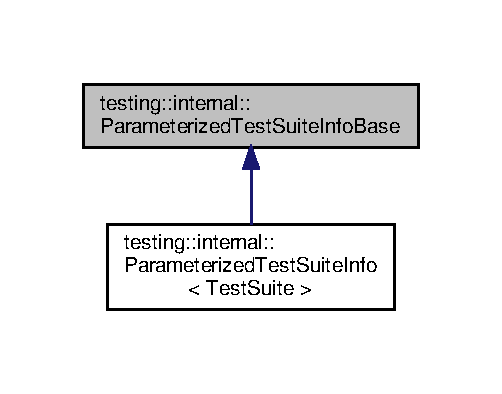
\includegraphics[width=241pt]{classtesting_1_1internal_1_1ParameterizedTestSuiteInfoBase__inherit__graph}
\end{center}
\end{figure}
\subsection*{Public Member Functions}
\begin{DoxyCompactItemize}
\item 
virtual \hyperlink{classtesting_1_1internal_1_1ParameterizedTestSuiteInfoBase_ac2aa0664f56e84cacab823d345c7d67b}{$\sim$\+Parameterized\+Test\+Suite\+Info\+Base} ()
\item 
virtual const std\+::string \& \hyperlink{classtesting_1_1internal_1_1ParameterizedTestSuiteInfoBase_aa6e36241431dc72c251ecee9b637b4d3}{Get\+Test\+Suite\+Name} () const =0
\item 
virtual \hyperlink{namespacetesting_1_1internal_ab1114197d3c657d8b7f8e0c5caa12d00}{Type\+Id} \hyperlink{classtesting_1_1internal_1_1ParameterizedTestSuiteInfoBase_ac5bcbf8c50a44472d697e0c80b54387d}{Get\+Test\+Suite\+Type\+Id} () const =0
\item 
virtual void \hyperlink{classtesting_1_1internal_1_1ParameterizedTestSuiteInfoBase_a41d7d663014af0c1e614c5a61293cb5a}{Register\+Tests} ()=0
\end{DoxyCompactItemize}
\subsection*{Protected Member Functions}
\begin{DoxyCompactItemize}
\item 
\hyperlink{classtesting_1_1internal_1_1ParameterizedTestSuiteInfoBase_a3b50ae419b0de858f3ad9b8dd49989de}{Parameterized\+Test\+Suite\+Info\+Base} ()
\end{DoxyCompactItemize}
\subsection*{Private Member Functions}
\begin{DoxyCompactItemize}
\item 
\hyperlink{classtesting_1_1internal_1_1ParameterizedTestSuiteInfoBase_a49431b7df609223c2a7fea67367e1d00}{G\+T\+E\+S\+T\+\_\+\+D\+I\+S\+A\+L\+L\+O\+W\+\_\+\+C\+O\+P\+Y\+\_\+\+A\+N\+D\+\_\+\+A\+S\+S\+I\+G\+N\+\_\+} (\hyperlink{classtesting_1_1internal_1_1ParameterizedTestSuiteInfoBase}{Parameterized\+Test\+Suite\+Info\+Base})
\end{DoxyCompactItemize}


\subsection{Constructor \& Destructor Documentation}
\mbox{\Hypertarget{classtesting_1_1internal_1_1ParameterizedTestSuiteInfoBase_ac2aa0664f56e84cacab823d345c7d67b}\label{classtesting_1_1internal_1_1ParameterizedTestSuiteInfoBase_ac2aa0664f56e84cacab823d345c7d67b}} 
\index{testing\+::internal\+::\+Parameterized\+Test\+Suite\+Info\+Base@{testing\+::internal\+::\+Parameterized\+Test\+Suite\+Info\+Base}!````~Parameterized\+Test\+Suite\+Info\+Base@{$\sim$\+Parameterized\+Test\+Suite\+Info\+Base}}
\index{````~Parameterized\+Test\+Suite\+Info\+Base@{$\sim$\+Parameterized\+Test\+Suite\+Info\+Base}!testing\+::internal\+::\+Parameterized\+Test\+Suite\+Info\+Base@{testing\+::internal\+::\+Parameterized\+Test\+Suite\+Info\+Base}}
\subsubsection{\texorpdfstring{$\sim$\+Parameterized\+Test\+Suite\+Info\+Base()}{~ParameterizedTestSuiteInfoBase()}}
{\footnotesize\ttfamily virtual testing\+::internal\+::\+Parameterized\+Test\+Suite\+Info\+Base\+::$\sim$\+Parameterized\+Test\+Suite\+Info\+Base (\begin{DoxyParamCaption}{ }\end{DoxyParamCaption})\hspace{0.3cm}{\ttfamily [inline]}, {\ttfamily [virtual]}}

\mbox{\Hypertarget{classtesting_1_1internal_1_1ParameterizedTestSuiteInfoBase_a3b50ae419b0de858f3ad9b8dd49989de}\label{classtesting_1_1internal_1_1ParameterizedTestSuiteInfoBase_a3b50ae419b0de858f3ad9b8dd49989de}} 
\index{testing\+::internal\+::\+Parameterized\+Test\+Suite\+Info\+Base@{testing\+::internal\+::\+Parameterized\+Test\+Suite\+Info\+Base}!Parameterized\+Test\+Suite\+Info\+Base@{Parameterized\+Test\+Suite\+Info\+Base}}
\index{Parameterized\+Test\+Suite\+Info\+Base@{Parameterized\+Test\+Suite\+Info\+Base}!testing\+::internal\+::\+Parameterized\+Test\+Suite\+Info\+Base@{testing\+::internal\+::\+Parameterized\+Test\+Suite\+Info\+Base}}
\subsubsection{\texorpdfstring{Parameterized\+Test\+Suite\+Info\+Base()}{ParameterizedTestSuiteInfoBase()}}
{\footnotesize\ttfamily testing\+::internal\+::\+Parameterized\+Test\+Suite\+Info\+Base\+::\+Parameterized\+Test\+Suite\+Info\+Base (\begin{DoxyParamCaption}{ }\end{DoxyParamCaption})\hspace{0.3cm}{\ttfamily [inline]}, {\ttfamily [protected]}}



\subsection{Member Function Documentation}
\mbox{\Hypertarget{classtesting_1_1internal_1_1ParameterizedTestSuiteInfoBase_aa6e36241431dc72c251ecee9b637b4d3}\label{classtesting_1_1internal_1_1ParameterizedTestSuiteInfoBase_aa6e36241431dc72c251ecee9b637b4d3}} 
\index{testing\+::internal\+::\+Parameterized\+Test\+Suite\+Info\+Base@{testing\+::internal\+::\+Parameterized\+Test\+Suite\+Info\+Base}!Get\+Test\+Suite\+Name@{Get\+Test\+Suite\+Name}}
\index{Get\+Test\+Suite\+Name@{Get\+Test\+Suite\+Name}!testing\+::internal\+::\+Parameterized\+Test\+Suite\+Info\+Base@{testing\+::internal\+::\+Parameterized\+Test\+Suite\+Info\+Base}}
\subsubsection{\texorpdfstring{Get\+Test\+Suite\+Name()}{GetTestSuiteName()}}
{\footnotesize\ttfamily virtual const std\+::string\& testing\+::internal\+::\+Parameterized\+Test\+Suite\+Info\+Base\+::\+Get\+Test\+Suite\+Name (\begin{DoxyParamCaption}{ }\end{DoxyParamCaption}) const\hspace{0.3cm}{\ttfamily [pure virtual]}}



Implemented in \hyperlink{classtesting_1_1internal_1_1ParameterizedTestSuiteInfo_a4a5ddc2cd0404438c2b4d405cd0e706c}{testing\+::internal\+::\+Parameterized\+Test\+Suite\+Info$<$ Test\+Suite $>$}.

\mbox{\Hypertarget{classtesting_1_1internal_1_1ParameterizedTestSuiteInfoBase_ac5bcbf8c50a44472d697e0c80b54387d}\label{classtesting_1_1internal_1_1ParameterizedTestSuiteInfoBase_ac5bcbf8c50a44472d697e0c80b54387d}} 
\index{testing\+::internal\+::\+Parameterized\+Test\+Suite\+Info\+Base@{testing\+::internal\+::\+Parameterized\+Test\+Suite\+Info\+Base}!Get\+Test\+Suite\+Type\+Id@{Get\+Test\+Suite\+Type\+Id}}
\index{Get\+Test\+Suite\+Type\+Id@{Get\+Test\+Suite\+Type\+Id}!testing\+::internal\+::\+Parameterized\+Test\+Suite\+Info\+Base@{testing\+::internal\+::\+Parameterized\+Test\+Suite\+Info\+Base}}
\subsubsection{\texorpdfstring{Get\+Test\+Suite\+Type\+Id()}{GetTestSuiteTypeId()}}
{\footnotesize\ttfamily virtual \hyperlink{namespacetesting_1_1internal_ab1114197d3c657d8b7f8e0c5caa12d00}{Type\+Id} testing\+::internal\+::\+Parameterized\+Test\+Suite\+Info\+Base\+::\+Get\+Test\+Suite\+Type\+Id (\begin{DoxyParamCaption}{ }\end{DoxyParamCaption}) const\hspace{0.3cm}{\ttfamily [pure virtual]}}



Implemented in \hyperlink{classtesting_1_1internal_1_1ParameterizedTestSuiteInfo_af488d1d7c1889a250acff2ea6eba4c84}{testing\+::internal\+::\+Parameterized\+Test\+Suite\+Info$<$ Test\+Suite $>$}.

\mbox{\Hypertarget{classtesting_1_1internal_1_1ParameterizedTestSuiteInfoBase_a49431b7df609223c2a7fea67367e1d00}\label{classtesting_1_1internal_1_1ParameterizedTestSuiteInfoBase_a49431b7df609223c2a7fea67367e1d00}} 
\index{testing\+::internal\+::\+Parameterized\+Test\+Suite\+Info\+Base@{testing\+::internal\+::\+Parameterized\+Test\+Suite\+Info\+Base}!G\+T\+E\+S\+T\+\_\+\+D\+I\+S\+A\+L\+L\+O\+W\+\_\+\+C\+O\+P\+Y\+\_\+\+A\+N\+D\+\_\+\+A\+S\+S\+I\+G\+N\+\_\+@{G\+T\+E\+S\+T\+\_\+\+D\+I\+S\+A\+L\+L\+O\+W\+\_\+\+C\+O\+P\+Y\+\_\+\+A\+N\+D\+\_\+\+A\+S\+S\+I\+G\+N\+\_\+}}
\index{G\+T\+E\+S\+T\+\_\+\+D\+I\+S\+A\+L\+L\+O\+W\+\_\+\+C\+O\+P\+Y\+\_\+\+A\+N\+D\+\_\+\+A\+S\+S\+I\+G\+N\+\_\+@{G\+T\+E\+S\+T\+\_\+\+D\+I\+S\+A\+L\+L\+O\+W\+\_\+\+C\+O\+P\+Y\+\_\+\+A\+N\+D\+\_\+\+A\+S\+S\+I\+G\+N\+\_\+}!testing\+::internal\+::\+Parameterized\+Test\+Suite\+Info\+Base@{testing\+::internal\+::\+Parameterized\+Test\+Suite\+Info\+Base}}
\subsubsection{\texorpdfstring{G\+T\+E\+S\+T\+\_\+\+D\+I\+S\+A\+L\+L\+O\+W\+\_\+\+C\+O\+P\+Y\+\_\+\+A\+N\+D\+\_\+\+A\+S\+S\+I\+G\+N\+\_\+()}{GTEST\_DISALLOW\_COPY\_AND\_ASSIGN\_()}}
{\footnotesize\ttfamily testing\+::internal\+::\+Parameterized\+Test\+Suite\+Info\+Base\+::\+G\+T\+E\+S\+T\+\_\+\+D\+I\+S\+A\+L\+L\+O\+W\+\_\+\+C\+O\+P\+Y\+\_\+\+A\+N\+D\+\_\+\+A\+S\+S\+I\+G\+N\+\_\+ (\begin{DoxyParamCaption}\item[{\hyperlink{classtesting_1_1internal_1_1ParameterizedTestSuiteInfoBase}{Parameterized\+Test\+Suite\+Info\+Base}}]{ }\end{DoxyParamCaption})\hspace{0.3cm}{\ttfamily [private]}}

\mbox{\Hypertarget{classtesting_1_1internal_1_1ParameterizedTestSuiteInfoBase_a41d7d663014af0c1e614c5a61293cb5a}\label{classtesting_1_1internal_1_1ParameterizedTestSuiteInfoBase_a41d7d663014af0c1e614c5a61293cb5a}} 
\index{testing\+::internal\+::\+Parameterized\+Test\+Suite\+Info\+Base@{testing\+::internal\+::\+Parameterized\+Test\+Suite\+Info\+Base}!Register\+Tests@{Register\+Tests}}
\index{Register\+Tests@{Register\+Tests}!testing\+::internal\+::\+Parameterized\+Test\+Suite\+Info\+Base@{testing\+::internal\+::\+Parameterized\+Test\+Suite\+Info\+Base}}
\subsubsection{\texorpdfstring{Register\+Tests()}{RegisterTests()}}
{\footnotesize\ttfamily virtual void testing\+::internal\+::\+Parameterized\+Test\+Suite\+Info\+Base\+::\+Register\+Tests (\begin{DoxyParamCaption}{ }\end{DoxyParamCaption})\hspace{0.3cm}{\ttfamily [pure virtual]}}



Implemented in \hyperlink{classtesting_1_1internal_1_1ParameterizedTestSuiteInfo_a8c0af866d3c291a63d3f4581ccd452d1}{testing\+::internal\+::\+Parameterized\+Test\+Suite\+Info$<$ Test\+Suite $>$}.



The documentation for this class was generated from the following file\+:\begin{DoxyCompactItemize}
\item 
tests/googletest/include/gtest/internal/\hyperlink{gtest-param-util_8h}{gtest-\/param-\/util.\+h}\end{DoxyCompactItemize}

\hypertarget{classtesting_1_1internal_1_1ParameterizedTestSuiteRegistry}{}\section{testing\+:\+:internal\+:\+:Parameterized\+Test\+Suite\+Registry Class Reference}
\label{classtesting_1_1internal_1_1ParameterizedTestSuiteRegistry}\index{testing\+::internal\+::\+Parameterized\+Test\+Suite\+Registry@{testing\+::internal\+::\+Parameterized\+Test\+Suite\+Registry}}


{\ttfamily \#include $<$gtest-\/param-\/util.\+h$>$}

\subsection*{Public Member Functions}
\begin{DoxyCompactItemize}
\item 
\hyperlink{classtesting_1_1internal_1_1ParameterizedTestSuiteRegistry_ae3827c085ed16faaa9197486513292c0}{Parameterized\+Test\+Suite\+Registry} ()
\item 
\hyperlink{classtesting_1_1internal_1_1ParameterizedTestSuiteRegistry_ab29f7a321883945d7f86f3292c100eb5}{$\sim$\+Parameterized\+Test\+Suite\+Registry} ()
\item 
{\footnotesize template$<$class Test\+Suite $>$ }\\\hyperlink{classtesting_1_1internal_1_1ParameterizedTestSuiteInfo}{Parameterized\+Test\+Suite\+Info}$<$ \hyperlink{classtesting_1_1TestSuite}{Test\+Suite} $>$ $\ast$ \hyperlink{classtesting_1_1internal_1_1ParameterizedTestSuiteRegistry_a89ef6dd228f4188e1928513e860580d0}{Get\+Test\+Suite\+Pattern\+Holder} (const char $\ast$test\+\_\+suite\+\_\+name, \hyperlink{structtesting_1_1internal_1_1CodeLocation}{Code\+Location} code\+\_\+location)
\item 
void \hyperlink{classtesting_1_1internal_1_1ParameterizedTestSuiteRegistry_a44c2ee0296de42dc6ca7abbf48d00495}{Register\+Tests} ()
\item 
{\footnotesize template$<$class Test\+Case $>$ }\\\hyperlink{namespacetesting_1_1internal_aac31682b6b41997d6cc610a5787dc8bc}{Parameterized\+Test\+Case\+Info}$<$ Test\+Case $>$ $\ast$ \hyperlink{classtesting_1_1internal_1_1ParameterizedTestSuiteRegistry_a3fe06fb4e1b4194dae1fbcdf3560fbd3}{Get\+Test\+Case\+Pattern\+Holder} (const char $\ast$test\+\_\+case\+\_\+name, \hyperlink{structtesting_1_1internal_1_1CodeLocation}{Code\+Location} code\+\_\+location)
\end{DoxyCompactItemize}
\subsection*{Private Types}
\begin{DoxyCompactItemize}
\item 
using \hyperlink{classtesting_1_1internal_1_1ParameterizedTestSuiteRegistry_a39a8d3dfa91cb48329bfcf0853f0e72b}{Test\+Suite\+Info\+Container} = \+::std\+::vector$<$ \hyperlink{classtesting_1_1internal_1_1ParameterizedTestSuiteInfoBase}{Parameterized\+Test\+Suite\+Info\+Base} $\ast$ $>$
\end{DoxyCompactItemize}
\subsection*{Private Member Functions}
\begin{DoxyCompactItemize}
\item 
\hyperlink{classtesting_1_1internal_1_1ParameterizedTestSuiteRegistry_ac1454da4ff60ddeda6b4e60f1b6ce606}{G\+T\+E\+S\+T\+\_\+\+D\+I\+S\+A\+L\+L\+O\+W\+\_\+\+C\+O\+P\+Y\+\_\+\+A\+N\+D\+\_\+\+A\+S\+S\+I\+G\+N\+\_\+} (\hyperlink{classtesting_1_1internal_1_1ParameterizedTestSuiteRegistry}{Parameterized\+Test\+Suite\+Registry})
\end{DoxyCompactItemize}
\subsection*{Private Attributes}
\begin{DoxyCompactItemize}
\item 
\hyperlink{classtesting_1_1internal_1_1ParameterizedTestSuiteRegistry_a39a8d3dfa91cb48329bfcf0853f0e72b}{Test\+Suite\+Info\+Container} \hyperlink{classtesting_1_1internal_1_1ParameterizedTestSuiteRegistry_afb0271d017a518724a075986bd16c69c}{test\+\_\+suite\+\_\+infos\+\_\+}
\end{DoxyCompactItemize}


\subsection{Member Typedef Documentation}
\mbox{\Hypertarget{classtesting_1_1internal_1_1ParameterizedTestSuiteRegistry_a39a8d3dfa91cb48329bfcf0853f0e72b}\label{classtesting_1_1internal_1_1ParameterizedTestSuiteRegistry_a39a8d3dfa91cb48329bfcf0853f0e72b}} 
\index{testing\+::internal\+::\+Parameterized\+Test\+Suite\+Registry@{testing\+::internal\+::\+Parameterized\+Test\+Suite\+Registry}!Test\+Suite\+Info\+Container@{Test\+Suite\+Info\+Container}}
\index{Test\+Suite\+Info\+Container@{Test\+Suite\+Info\+Container}!testing\+::internal\+::\+Parameterized\+Test\+Suite\+Registry@{testing\+::internal\+::\+Parameterized\+Test\+Suite\+Registry}}
\subsubsection{\texorpdfstring{Test\+Suite\+Info\+Container}{TestSuiteInfoContainer}}
{\footnotesize\ttfamily using \hyperlink{classtesting_1_1internal_1_1ParameterizedTestSuiteRegistry_a39a8d3dfa91cb48329bfcf0853f0e72b}{testing\+::internal\+::\+Parameterized\+Test\+Suite\+Registry\+::\+Test\+Suite\+Info\+Container} =  \+::std\+::vector$<$\hyperlink{classtesting_1_1internal_1_1ParameterizedTestSuiteInfoBase}{Parameterized\+Test\+Suite\+Info\+Base}$\ast$$>$\hspace{0.3cm}{\ttfamily [private]}}



\subsection{Constructor \& Destructor Documentation}
\mbox{\Hypertarget{classtesting_1_1internal_1_1ParameterizedTestSuiteRegistry_ae3827c085ed16faaa9197486513292c0}\label{classtesting_1_1internal_1_1ParameterizedTestSuiteRegistry_ae3827c085ed16faaa9197486513292c0}} 
\index{testing\+::internal\+::\+Parameterized\+Test\+Suite\+Registry@{testing\+::internal\+::\+Parameterized\+Test\+Suite\+Registry}!Parameterized\+Test\+Suite\+Registry@{Parameterized\+Test\+Suite\+Registry}}
\index{Parameterized\+Test\+Suite\+Registry@{Parameterized\+Test\+Suite\+Registry}!testing\+::internal\+::\+Parameterized\+Test\+Suite\+Registry@{testing\+::internal\+::\+Parameterized\+Test\+Suite\+Registry}}
\subsubsection{\texorpdfstring{Parameterized\+Test\+Suite\+Registry()}{ParameterizedTestSuiteRegistry()}}
{\footnotesize\ttfamily testing\+::internal\+::\+Parameterized\+Test\+Suite\+Registry\+::\+Parameterized\+Test\+Suite\+Registry (\begin{DoxyParamCaption}{ }\end{DoxyParamCaption})\hspace{0.3cm}{\ttfamily [inline]}}

\mbox{\Hypertarget{classtesting_1_1internal_1_1ParameterizedTestSuiteRegistry_ab29f7a321883945d7f86f3292c100eb5}\label{classtesting_1_1internal_1_1ParameterizedTestSuiteRegistry_ab29f7a321883945d7f86f3292c100eb5}} 
\index{testing\+::internal\+::\+Parameterized\+Test\+Suite\+Registry@{testing\+::internal\+::\+Parameterized\+Test\+Suite\+Registry}!````~Parameterized\+Test\+Suite\+Registry@{$\sim$\+Parameterized\+Test\+Suite\+Registry}}
\index{````~Parameterized\+Test\+Suite\+Registry@{$\sim$\+Parameterized\+Test\+Suite\+Registry}!testing\+::internal\+::\+Parameterized\+Test\+Suite\+Registry@{testing\+::internal\+::\+Parameterized\+Test\+Suite\+Registry}}
\subsubsection{\texorpdfstring{$\sim$\+Parameterized\+Test\+Suite\+Registry()}{~ParameterizedTestSuiteRegistry()}}
{\footnotesize\ttfamily testing\+::internal\+::\+Parameterized\+Test\+Suite\+Registry\+::$\sim$\+Parameterized\+Test\+Suite\+Registry (\begin{DoxyParamCaption}{ }\end{DoxyParamCaption})\hspace{0.3cm}{\ttfamily [inline]}}



\subsection{Member Function Documentation}
\mbox{\Hypertarget{classtesting_1_1internal_1_1ParameterizedTestSuiteRegistry_a3fe06fb4e1b4194dae1fbcdf3560fbd3}\label{classtesting_1_1internal_1_1ParameterizedTestSuiteRegistry_a3fe06fb4e1b4194dae1fbcdf3560fbd3}} 
\index{testing\+::internal\+::\+Parameterized\+Test\+Suite\+Registry@{testing\+::internal\+::\+Parameterized\+Test\+Suite\+Registry}!Get\+Test\+Case\+Pattern\+Holder@{Get\+Test\+Case\+Pattern\+Holder}}
\index{Get\+Test\+Case\+Pattern\+Holder@{Get\+Test\+Case\+Pattern\+Holder}!testing\+::internal\+::\+Parameterized\+Test\+Suite\+Registry@{testing\+::internal\+::\+Parameterized\+Test\+Suite\+Registry}}
\subsubsection{\texorpdfstring{Get\+Test\+Case\+Pattern\+Holder()}{GetTestCasePatternHolder()}}
{\footnotesize\ttfamily template$<$class Test\+Case $>$ \\
\hyperlink{namespacetesting_1_1internal_aac31682b6b41997d6cc610a5787dc8bc}{Parameterized\+Test\+Case\+Info}$<$Test\+Case$>$$\ast$ testing\+::internal\+::\+Parameterized\+Test\+Suite\+Registry\+::\+Get\+Test\+Case\+Pattern\+Holder (\begin{DoxyParamCaption}\item[{const char $\ast$}]{test\+\_\+case\+\_\+name,  }\item[{\hyperlink{structtesting_1_1internal_1_1CodeLocation}{Code\+Location}}]{code\+\_\+location }\end{DoxyParamCaption})\hspace{0.3cm}{\ttfamily [inline]}}

\mbox{\Hypertarget{classtesting_1_1internal_1_1ParameterizedTestSuiteRegistry_a89ef6dd228f4188e1928513e860580d0}\label{classtesting_1_1internal_1_1ParameterizedTestSuiteRegistry_a89ef6dd228f4188e1928513e860580d0}} 
\index{testing\+::internal\+::\+Parameterized\+Test\+Suite\+Registry@{testing\+::internal\+::\+Parameterized\+Test\+Suite\+Registry}!Get\+Test\+Suite\+Pattern\+Holder@{Get\+Test\+Suite\+Pattern\+Holder}}
\index{Get\+Test\+Suite\+Pattern\+Holder@{Get\+Test\+Suite\+Pattern\+Holder}!testing\+::internal\+::\+Parameterized\+Test\+Suite\+Registry@{testing\+::internal\+::\+Parameterized\+Test\+Suite\+Registry}}
\subsubsection{\texorpdfstring{Get\+Test\+Suite\+Pattern\+Holder()}{GetTestSuitePatternHolder()}}
{\footnotesize\ttfamily template$<$class Test\+Suite $>$ \\
\hyperlink{classtesting_1_1internal_1_1ParameterizedTestSuiteInfo}{Parameterized\+Test\+Suite\+Info}$<$\hyperlink{classtesting_1_1TestSuite}{Test\+Suite}$>$$\ast$ testing\+::internal\+::\+Parameterized\+Test\+Suite\+Registry\+::\+Get\+Test\+Suite\+Pattern\+Holder (\begin{DoxyParamCaption}\item[{const char $\ast$}]{test\+\_\+suite\+\_\+name,  }\item[{\hyperlink{structtesting_1_1internal_1_1CodeLocation}{Code\+Location}}]{code\+\_\+location }\end{DoxyParamCaption})\hspace{0.3cm}{\ttfamily [inline]}}

\mbox{\Hypertarget{classtesting_1_1internal_1_1ParameterizedTestSuiteRegistry_ac1454da4ff60ddeda6b4e60f1b6ce606}\label{classtesting_1_1internal_1_1ParameterizedTestSuiteRegistry_ac1454da4ff60ddeda6b4e60f1b6ce606}} 
\index{testing\+::internal\+::\+Parameterized\+Test\+Suite\+Registry@{testing\+::internal\+::\+Parameterized\+Test\+Suite\+Registry}!G\+T\+E\+S\+T\+\_\+\+D\+I\+S\+A\+L\+L\+O\+W\+\_\+\+C\+O\+P\+Y\+\_\+\+A\+N\+D\+\_\+\+A\+S\+S\+I\+G\+N\+\_\+@{G\+T\+E\+S\+T\+\_\+\+D\+I\+S\+A\+L\+L\+O\+W\+\_\+\+C\+O\+P\+Y\+\_\+\+A\+N\+D\+\_\+\+A\+S\+S\+I\+G\+N\+\_\+}}
\index{G\+T\+E\+S\+T\+\_\+\+D\+I\+S\+A\+L\+L\+O\+W\+\_\+\+C\+O\+P\+Y\+\_\+\+A\+N\+D\+\_\+\+A\+S\+S\+I\+G\+N\+\_\+@{G\+T\+E\+S\+T\+\_\+\+D\+I\+S\+A\+L\+L\+O\+W\+\_\+\+C\+O\+P\+Y\+\_\+\+A\+N\+D\+\_\+\+A\+S\+S\+I\+G\+N\+\_\+}!testing\+::internal\+::\+Parameterized\+Test\+Suite\+Registry@{testing\+::internal\+::\+Parameterized\+Test\+Suite\+Registry}}
\subsubsection{\texorpdfstring{G\+T\+E\+S\+T\+\_\+\+D\+I\+S\+A\+L\+L\+O\+W\+\_\+\+C\+O\+P\+Y\+\_\+\+A\+N\+D\+\_\+\+A\+S\+S\+I\+G\+N\+\_\+()}{GTEST\_DISALLOW\_COPY\_AND\_ASSIGN\_()}}
{\footnotesize\ttfamily testing\+::internal\+::\+Parameterized\+Test\+Suite\+Registry\+::\+G\+T\+E\+S\+T\+\_\+\+D\+I\+S\+A\+L\+L\+O\+W\+\_\+\+C\+O\+P\+Y\+\_\+\+A\+N\+D\+\_\+\+A\+S\+S\+I\+G\+N\+\_\+ (\begin{DoxyParamCaption}\item[{\hyperlink{classtesting_1_1internal_1_1ParameterizedTestSuiteRegistry}{Parameterized\+Test\+Suite\+Registry}}]{ }\end{DoxyParamCaption})\hspace{0.3cm}{\ttfamily [private]}}

\mbox{\Hypertarget{classtesting_1_1internal_1_1ParameterizedTestSuiteRegistry_a44c2ee0296de42dc6ca7abbf48d00495}\label{classtesting_1_1internal_1_1ParameterizedTestSuiteRegistry_a44c2ee0296de42dc6ca7abbf48d00495}} 
\index{testing\+::internal\+::\+Parameterized\+Test\+Suite\+Registry@{testing\+::internal\+::\+Parameterized\+Test\+Suite\+Registry}!Register\+Tests@{Register\+Tests}}
\index{Register\+Tests@{Register\+Tests}!testing\+::internal\+::\+Parameterized\+Test\+Suite\+Registry@{testing\+::internal\+::\+Parameterized\+Test\+Suite\+Registry}}
\subsubsection{\texorpdfstring{Register\+Tests()}{RegisterTests()}}
{\footnotesize\ttfamily void testing\+::internal\+::\+Parameterized\+Test\+Suite\+Registry\+::\+Register\+Tests (\begin{DoxyParamCaption}{ }\end{DoxyParamCaption})\hspace{0.3cm}{\ttfamily [inline]}}



\subsection{Member Data Documentation}
\mbox{\Hypertarget{classtesting_1_1internal_1_1ParameterizedTestSuiteRegistry_afb0271d017a518724a075986bd16c69c}\label{classtesting_1_1internal_1_1ParameterizedTestSuiteRegistry_afb0271d017a518724a075986bd16c69c}} 
\index{testing\+::internal\+::\+Parameterized\+Test\+Suite\+Registry@{testing\+::internal\+::\+Parameterized\+Test\+Suite\+Registry}!test\+\_\+suite\+\_\+infos\+\_\+@{test\+\_\+suite\+\_\+infos\+\_\+}}
\index{test\+\_\+suite\+\_\+infos\+\_\+@{test\+\_\+suite\+\_\+infos\+\_\+}!testing\+::internal\+::\+Parameterized\+Test\+Suite\+Registry@{testing\+::internal\+::\+Parameterized\+Test\+Suite\+Registry}}
\subsubsection{\texorpdfstring{test\+\_\+suite\+\_\+infos\+\_\+}{test\_suite\_infos\_}}
{\footnotesize\ttfamily \hyperlink{classtesting_1_1internal_1_1ParameterizedTestSuiteRegistry_a39a8d3dfa91cb48329bfcf0853f0e72b}{Test\+Suite\+Info\+Container} testing\+::internal\+::\+Parameterized\+Test\+Suite\+Registry\+::test\+\_\+suite\+\_\+infos\+\_\+\hspace{0.3cm}{\ttfamily [private]}}



The documentation for this class was generated from the following file\+:\begin{DoxyCompactItemize}
\item 
tests/googletest/include/gtest/internal/\hyperlink{gtest-param-util_8h}{gtest-\/param-\/util.\+h}\end{DoxyCompactItemize}

\hypertarget{classtesting_1_1internal_1_1ParamGenerator}{}\section{testing\+:\+:internal\+:\+:Param\+Generator$<$ T $>$ Class Template Reference}
\label{classtesting_1_1internal_1_1ParamGenerator}\index{testing\+::internal\+::\+Param\+Generator$<$ T $>$@{testing\+::internal\+::\+Param\+Generator$<$ T $>$}}


{\ttfamily \#include $<$gtest-\/param-\/util.\+h$>$}

\subsection*{Public Types}
\begin{DoxyCompactItemize}
\item 
typedef \hyperlink{classtesting_1_1internal_1_1ParamIterator}{Param\+Iterator}$<$ T $>$ \hyperlink{classtesting_1_1internal_1_1ParamGenerator_a448b08a8eaae1f1d27840d4dbd66c357}{iterator}
\end{DoxyCompactItemize}
\subsection*{Public Member Functions}
\begin{DoxyCompactItemize}
\item 
\hyperlink{classtesting_1_1internal_1_1ParamGenerator_a6b017d4d030927714d495ee95ae92fbc}{Param\+Generator} (\hyperlink{classtesting_1_1internal_1_1ParamGeneratorInterface}{Param\+Generator\+Interface}$<$ T $>$ $\ast$impl)
\item 
\hyperlink{classtesting_1_1internal_1_1ParamGenerator_a5891d25c31919b3099489f8bbcd58b5e}{Param\+Generator} (const \hyperlink{classtesting_1_1internal_1_1ParamGenerator}{Param\+Generator} \&other)
\item 
\hyperlink{classtesting_1_1internal_1_1ParamGenerator}{Param\+Generator} \& \hyperlink{classtesting_1_1internal_1_1ParamGenerator_a590a03c6e0a3a3ac6279943ad1f01dc8}{operator=} (const \hyperlink{classtesting_1_1internal_1_1ParamGenerator}{Param\+Generator} \&other)
\item 
\hyperlink{classtesting_1_1internal_1_1ParamGenerator_a448b08a8eaae1f1d27840d4dbd66c357}{iterator} \hyperlink{classtesting_1_1internal_1_1ParamGenerator_a14e735c8bd113556ae905a560cd2d607}{begin} () const
\item 
\hyperlink{classtesting_1_1internal_1_1ParamGenerator_a448b08a8eaae1f1d27840d4dbd66c357}{iterator} \hyperlink{classtesting_1_1internal_1_1ParamGenerator_aaf8f75df1099a07ff771a550b48f9fbe}{end} () const
\end{DoxyCompactItemize}
\subsection*{Private Attributes}
\begin{DoxyCompactItemize}
\item 
std\+::shared\+\_\+ptr$<$ const \hyperlink{classtesting_1_1internal_1_1ParamGeneratorInterface}{Param\+Generator\+Interface}$<$ T $>$ $>$ \hyperlink{classtesting_1_1internal_1_1ParamGenerator_a2ea0b72d470d5a961272c2b818a3f78d}{impl\+\_\+}
\end{DoxyCompactItemize}


\subsection{Member Typedef Documentation}
\mbox{\Hypertarget{classtesting_1_1internal_1_1ParamGenerator_a448b08a8eaae1f1d27840d4dbd66c357}\label{classtesting_1_1internal_1_1ParamGenerator_a448b08a8eaae1f1d27840d4dbd66c357}} 
\index{testing\+::internal\+::\+Param\+Generator@{testing\+::internal\+::\+Param\+Generator}!iterator@{iterator}}
\index{iterator@{iterator}!testing\+::internal\+::\+Param\+Generator@{testing\+::internal\+::\+Param\+Generator}}
\subsubsection{\texorpdfstring{iterator}{iterator}}
{\footnotesize\ttfamily template$<$typename T$>$ \\
typedef \hyperlink{classtesting_1_1internal_1_1ParamIterator}{Param\+Iterator}$<$T$>$ \hyperlink{classtesting_1_1internal_1_1ParamGenerator}{testing\+::internal\+::\+Param\+Generator}$<$ T $>$\+::\hyperlink{classtesting_1_1internal_1_1ParamGenerator_a448b08a8eaae1f1d27840d4dbd66c357}{iterator}}



\subsection{Constructor \& Destructor Documentation}
\mbox{\Hypertarget{classtesting_1_1internal_1_1ParamGenerator_a6b017d4d030927714d495ee95ae92fbc}\label{classtesting_1_1internal_1_1ParamGenerator_a6b017d4d030927714d495ee95ae92fbc}} 
\index{testing\+::internal\+::\+Param\+Generator@{testing\+::internal\+::\+Param\+Generator}!Param\+Generator@{Param\+Generator}}
\index{Param\+Generator@{Param\+Generator}!testing\+::internal\+::\+Param\+Generator@{testing\+::internal\+::\+Param\+Generator}}
\subsubsection{\texorpdfstring{Param\+Generator()}{ParamGenerator()}\hspace{0.1cm}{\footnotesize\ttfamily [1/2]}}
{\footnotesize\ttfamily template$<$typename T$>$ \\
\hyperlink{classtesting_1_1internal_1_1ParamGenerator}{testing\+::internal\+::\+Param\+Generator}$<$ T $>$\+::\hyperlink{classtesting_1_1internal_1_1ParamGenerator}{Param\+Generator} (\begin{DoxyParamCaption}\item[{\hyperlink{classtesting_1_1internal_1_1ParamGeneratorInterface}{Param\+Generator\+Interface}$<$ T $>$ $\ast$}]{impl }\end{DoxyParamCaption})\hspace{0.3cm}{\ttfamily [inline]}, {\ttfamily [explicit]}}

\mbox{\Hypertarget{classtesting_1_1internal_1_1ParamGenerator_a5891d25c31919b3099489f8bbcd58b5e}\label{classtesting_1_1internal_1_1ParamGenerator_a5891d25c31919b3099489f8bbcd58b5e}} 
\index{testing\+::internal\+::\+Param\+Generator@{testing\+::internal\+::\+Param\+Generator}!Param\+Generator@{Param\+Generator}}
\index{Param\+Generator@{Param\+Generator}!testing\+::internal\+::\+Param\+Generator@{testing\+::internal\+::\+Param\+Generator}}
\subsubsection{\texorpdfstring{Param\+Generator()}{ParamGenerator()}\hspace{0.1cm}{\footnotesize\ttfamily [2/2]}}
{\footnotesize\ttfamily template$<$typename T$>$ \\
\hyperlink{classtesting_1_1internal_1_1ParamGenerator}{testing\+::internal\+::\+Param\+Generator}$<$ T $>$\+::\hyperlink{classtesting_1_1internal_1_1ParamGenerator}{Param\+Generator} (\begin{DoxyParamCaption}\item[{const \hyperlink{classtesting_1_1internal_1_1ParamGenerator}{Param\+Generator}$<$ T $>$ \&}]{other }\end{DoxyParamCaption})\hspace{0.3cm}{\ttfamily [inline]}}



\subsection{Member Function Documentation}
\mbox{\Hypertarget{classtesting_1_1internal_1_1ParamGenerator_a14e735c8bd113556ae905a560cd2d607}\label{classtesting_1_1internal_1_1ParamGenerator_a14e735c8bd113556ae905a560cd2d607}} 
\index{testing\+::internal\+::\+Param\+Generator@{testing\+::internal\+::\+Param\+Generator}!begin@{begin}}
\index{begin@{begin}!testing\+::internal\+::\+Param\+Generator@{testing\+::internal\+::\+Param\+Generator}}
\subsubsection{\texorpdfstring{begin()}{begin()}}
{\footnotesize\ttfamily template$<$typename T$>$ \\
\hyperlink{classtesting_1_1internal_1_1ParamGenerator_a448b08a8eaae1f1d27840d4dbd66c357}{iterator} \hyperlink{classtesting_1_1internal_1_1ParamGenerator}{testing\+::internal\+::\+Param\+Generator}$<$ T $>$\+::begin (\begin{DoxyParamCaption}{ }\end{DoxyParamCaption}) const\hspace{0.3cm}{\ttfamily [inline]}}

\mbox{\Hypertarget{classtesting_1_1internal_1_1ParamGenerator_aaf8f75df1099a07ff771a550b48f9fbe}\label{classtesting_1_1internal_1_1ParamGenerator_aaf8f75df1099a07ff771a550b48f9fbe}} 
\index{testing\+::internal\+::\+Param\+Generator@{testing\+::internal\+::\+Param\+Generator}!end@{end}}
\index{end@{end}!testing\+::internal\+::\+Param\+Generator@{testing\+::internal\+::\+Param\+Generator}}
\subsubsection{\texorpdfstring{end()}{end()}}
{\footnotesize\ttfamily template$<$typename T$>$ \\
\hyperlink{classtesting_1_1internal_1_1ParamGenerator_a448b08a8eaae1f1d27840d4dbd66c357}{iterator} \hyperlink{classtesting_1_1internal_1_1ParamGenerator}{testing\+::internal\+::\+Param\+Generator}$<$ T $>$\+::end (\begin{DoxyParamCaption}{ }\end{DoxyParamCaption}) const\hspace{0.3cm}{\ttfamily [inline]}}

\mbox{\Hypertarget{classtesting_1_1internal_1_1ParamGenerator_a590a03c6e0a3a3ac6279943ad1f01dc8}\label{classtesting_1_1internal_1_1ParamGenerator_a590a03c6e0a3a3ac6279943ad1f01dc8}} 
\index{testing\+::internal\+::\+Param\+Generator@{testing\+::internal\+::\+Param\+Generator}!operator=@{operator=}}
\index{operator=@{operator=}!testing\+::internal\+::\+Param\+Generator@{testing\+::internal\+::\+Param\+Generator}}
\subsubsection{\texorpdfstring{operator=()}{operator=()}}
{\footnotesize\ttfamily template$<$typename T$>$ \\
\hyperlink{classtesting_1_1internal_1_1ParamGenerator}{Param\+Generator}\& \hyperlink{classtesting_1_1internal_1_1ParamGenerator}{testing\+::internal\+::\+Param\+Generator}$<$ T $>$\+::operator= (\begin{DoxyParamCaption}\item[{const \hyperlink{classtesting_1_1internal_1_1ParamGenerator}{Param\+Generator}$<$ T $>$ \&}]{other }\end{DoxyParamCaption})\hspace{0.3cm}{\ttfamily [inline]}}



\subsection{Member Data Documentation}
\mbox{\Hypertarget{classtesting_1_1internal_1_1ParamGenerator_a2ea0b72d470d5a961272c2b818a3f78d}\label{classtesting_1_1internal_1_1ParamGenerator_a2ea0b72d470d5a961272c2b818a3f78d}} 
\index{testing\+::internal\+::\+Param\+Generator@{testing\+::internal\+::\+Param\+Generator}!impl\+\_\+@{impl\+\_\+}}
\index{impl\+\_\+@{impl\+\_\+}!testing\+::internal\+::\+Param\+Generator@{testing\+::internal\+::\+Param\+Generator}}
\subsubsection{\texorpdfstring{impl\+\_\+}{impl\_}}
{\footnotesize\ttfamily template$<$typename T$>$ \\
std\+::shared\+\_\+ptr$<$const \hyperlink{classtesting_1_1internal_1_1ParamGeneratorInterface}{Param\+Generator\+Interface}$<$T$>$ $>$ \hyperlink{classtesting_1_1internal_1_1ParamGenerator}{testing\+::internal\+::\+Param\+Generator}$<$ T $>$\+::impl\+\_\+\hspace{0.3cm}{\ttfamily [private]}}



The documentation for this class was generated from the following file\+:\begin{DoxyCompactItemize}
\item 
tests/googletest/include/gtest/internal/\hyperlink{gtest-param-util_8h}{gtest-\/param-\/util.\+h}\end{DoxyCompactItemize}

\hypertarget{classtesting_1_1internal_1_1ParamGeneratorInterface}{}\section{testing\+:\+:internal\+:\+:Param\+Generator\+Interface$<$ T $>$ Class Template Reference}
\label{classtesting_1_1internal_1_1ParamGeneratorInterface}\index{testing\+::internal\+::\+Param\+Generator\+Interface$<$ T $>$@{testing\+::internal\+::\+Param\+Generator\+Interface$<$ T $>$}}


{\ttfamily \#include $<$gtest-\/param-\/util.\+h$>$}



Inheritance diagram for testing\+:\+:internal\+:\+:Param\+Generator\+Interface$<$ T $>$\+:\nopagebreak
\begin{figure}[H]
\begin{center}
\leavevmode
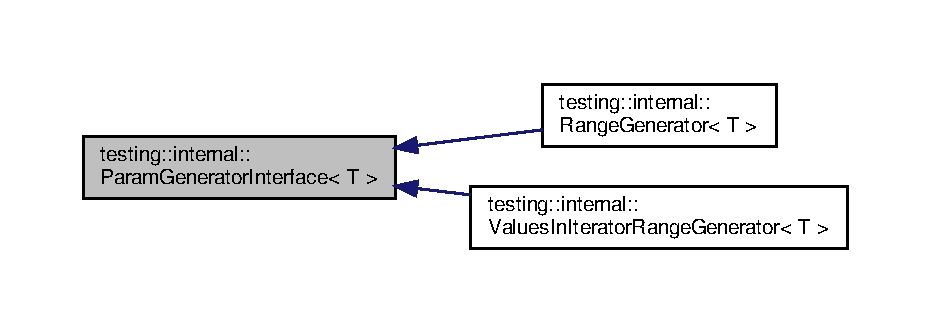
\includegraphics[width=350pt]{classtesting_1_1internal_1_1ParamGeneratorInterface__inherit__graph}
\end{center}
\end{figure}
\subsection*{Public Types}
\begin{DoxyCompactItemize}
\item 
typedef T \hyperlink{classtesting_1_1internal_1_1ParamGeneratorInterface_ab33d2ea424c50beaf503cb125b3cd003}{Param\+Type}
\end{DoxyCompactItemize}
\subsection*{Public Member Functions}
\begin{DoxyCompactItemize}
\item 
virtual \hyperlink{classtesting_1_1internal_1_1ParamGeneratorInterface_ac2767cb9ad2e292e291c4903323c6eff}{$\sim$\+Param\+Generator\+Interface} ()
\item 
virtual \hyperlink{classtesting_1_1internal_1_1ParamIteratorInterface}{Param\+Iterator\+Interface}$<$ T $>$ $\ast$ \hyperlink{classtesting_1_1internal_1_1ParamGeneratorInterface_ae1de83b16fe9a53c67778a026c6a9569}{Begin} () const =0
\item 
virtual \hyperlink{classtesting_1_1internal_1_1ParamIteratorInterface}{Param\+Iterator\+Interface}$<$ T $>$ $\ast$ \hyperlink{classtesting_1_1internal_1_1ParamGeneratorInterface_afa7211b74990e11d3fc7ad4e7113da4f}{End} () const =0
\end{DoxyCompactItemize}


\subsection{Member Typedef Documentation}
\mbox{\Hypertarget{classtesting_1_1internal_1_1ParamGeneratorInterface_ab33d2ea424c50beaf503cb125b3cd003}\label{classtesting_1_1internal_1_1ParamGeneratorInterface_ab33d2ea424c50beaf503cb125b3cd003}} 
\index{testing\+::internal\+::\+Param\+Generator\+Interface@{testing\+::internal\+::\+Param\+Generator\+Interface}!Param\+Type@{Param\+Type}}
\index{Param\+Type@{Param\+Type}!testing\+::internal\+::\+Param\+Generator\+Interface@{testing\+::internal\+::\+Param\+Generator\+Interface}}
\subsubsection{\texorpdfstring{Param\+Type}{ParamType}}
{\footnotesize\ttfamily template$<$typename T$>$ \\
typedef T \hyperlink{classtesting_1_1internal_1_1ParamGeneratorInterface}{testing\+::internal\+::\+Param\+Generator\+Interface}$<$ T $>$\+::\hyperlink{classtesting_1_1internal_1_1ParamGeneratorInterface_ab33d2ea424c50beaf503cb125b3cd003}{Param\+Type}}



\subsection{Constructor \& Destructor Documentation}
\mbox{\Hypertarget{classtesting_1_1internal_1_1ParamGeneratorInterface_ac2767cb9ad2e292e291c4903323c6eff}\label{classtesting_1_1internal_1_1ParamGeneratorInterface_ac2767cb9ad2e292e291c4903323c6eff}} 
\index{testing\+::internal\+::\+Param\+Generator\+Interface@{testing\+::internal\+::\+Param\+Generator\+Interface}!````~Param\+Generator\+Interface@{$\sim$\+Param\+Generator\+Interface}}
\index{````~Param\+Generator\+Interface@{$\sim$\+Param\+Generator\+Interface}!testing\+::internal\+::\+Param\+Generator\+Interface@{testing\+::internal\+::\+Param\+Generator\+Interface}}
\subsubsection{\texorpdfstring{$\sim$\+Param\+Generator\+Interface()}{~ParamGeneratorInterface()}}
{\footnotesize\ttfamily template$<$typename T$>$ \\
virtual \hyperlink{classtesting_1_1internal_1_1ParamGeneratorInterface}{testing\+::internal\+::\+Param\+Generator\+Interface}$<$ T $>$\+::$\sim$\hyperlink{classtesting_1_1internal_1_1ParamGeneratorInterface}{Param\+Generator\+Interface} (\begin{DoxyParamCaption}{ }\end{DoxyParamCaption})\hspace{0.3cm}{\ttfamily [inline]}, {\ttfamily [virtual]}}



\subsection{Member Function Documentation}
\mbox{\Hypertarget{classtesting_1_1internal_1_1ParamGeneratorInterface_ae1de83b16fe9a53c67778a026c6a9569}\label{classtesting_1_1internal_1_1ParamGeneratorInterface_ae1de83b16fe9a53c67778a026c6a9569}} 
\index{testing\+::internal\+::\+Param\+Generator\+Interface@{testing\+::internal\+::\+Param\+Generator\+Interface}!Begin@{Begin}}
\index{Begin@{Begin}!testing\+::internal\+::\+Param\+Generator\+Interface@{testing\+::internal\+::\+Param\+Generator\+Interface}}
\subsubsection{\texorpdfstring{Begin()}{Begin()}}
{\footnotesize\ttfamily template$<$typename T$>$ \\
virtual \hyperlink{classtesting_1_1internal_1_1ParamIteratorInterface}{Param\+Iterator\+Interface}$<$T$>$$\ast$ \hyperlink{classtesting_1_1internal_1_1ParamGeneratorInterface}{testing\+::internal\+::\+Param\+Generator\+Interface}$<$ T $>$\+::Begin (\begin{DoxyParamCaption}{ }\end{DoxyParamCaption}) const\hspace{0.3cm}{\ttfamily [pure virtual]}}



Implemented in \hyperlink{classtesting_1_1internal_1_1CartesianProductGenerator_ad2f1bc6289b6dd7e4b5f4fecbfdf2883}{testing\+::internal\+::\+Cartesian\+Product\+Generator$<$ T $>$}, \hyperlink{classtesting_1_1internal_1_1ValuesInIteratorRangeGenerator_a71ffed6f1deba05f11c9d45f6ab5b85d}{testing\+::internal\+::\+Values\+In\+Iterator\+Range\+Generator$<$ T $>$}, and \hyperlink{classtesting_1_1internal_1_1RangeGenerator_a502913fbcf14e89d5765dfb44f3c1295}{testing\+::internal\+::\+Range\+Generator$<$ T, Increment\+T $>$}.

\mbox{\Hypertarget{classtesting_1_1internal_1_1ParamGeneratorInterface_afa7211b74990e11d3fc7ad4e7113da4f}\label{classtesting_1_1internal_1_1ParamGeneratorInterface_afa7211b74990e11d3fc7ad4e7113da4f}} 
\index{testing\+::internal\+::\+Param\+Generator\+Interface@{testing\+::internal\+::\+Param\+Generator\+Interface}!End@{End}}
\index{End@{End}!testing\+::internal\+::\+Param\+Generator\+Interface@{testing\+::internal\+::\+Param\+Generator\+Interface}}
\subsubsection{\texorpdfstring{End()}{End()}}
{\footnotesize\ttfamily template$<$typename T$>$ \\
virtual \hyperlink{classtesting_1_1internal_1_1ParamIteratorInterface}{Param\+Iterator\+Interface}$<$T$>$$\ast$ \hyperlink{classtesting_1_1internal_1_1ParamGeneratorInterface}{testing\+::internal\+::\+Param\+Generator\+Interface}$<$ T $>$\+::End (\begin{DoxyParamCaption}{ }\end{DoxyParamCaption}) const\hspace{0.3cm}{\ttfamily [pure virtual]}}



Implemented in \hyperlink{classtesting_1_1internal_1_1CartesianProductGenerator_ae072dcf8400ac9dd5692e417262a664b}{testing\+::internal\+::\+Cartesian\+Product\+Generator$<$ T $>$}, \hyperlink{classtesting_1_1internal_1_1ValuesInIteratorRangeGenerator_a298cfb66a90b1a39c0cea3ca7ae1ece1}{testing\+::internal\+::\+Values\+In\+Iterator\+Range\+Generator$<$ T $>$}, and \hyperlink{classtesting_1_1internal_1_1RangeGenerator_ac112ca69567b9c47bf14554e0473e1e2}{testing\+::internal\+::\+Range\+Generator$<$ T, Increment\+T $>$}.



The documentation for this class was generated from the following file\+:\begin{DoxyCompactItemize}
\item 
tests/googletest/include/gtest/internal/\hyperlink{gtest-param-util_8h}{gtest-\/param-\/util.\+h}\end{DoxyCompactItemize}

\hypertarget{classtesting_1_1internal_1_1ParamIterator}{}\section{testing\+:\+:internal\+:\+:Param\+Iterator$<$ T $>$ Class Template Reference}
\label{classtesting_1_1internal_1_1ParamIterator}\index{testing\+::internal\+::\+Param\+Iterator$<$ T $>$@{testing\+::internal\+::\+Param\+Iterator$<$ T $>$}}


{\ttfamily \#include $<$gtest-\/param-\/util.\+h$>$}

\subsection*{Public Types}
\begin{DoxyCompactItemize}
\item 
typedef T \hyperlink{classtesting_1_1internal_1_1ParamIterator_a4afe3a68db0d0744753c8afe262e35df}{value\+\_\+type}
\item 
typedef const T \& \hyperlink{classtesting_1_1internal_1_1ParamIterator_ac96f133ffa06fc0f9faff5a1c7954382}{reference}
\item 
typedef ptrdiff\+\_\+t \hyperlink{classtesting_1_1internal_1_1ParamIterator_a6c37240a04ba3fc4c56f6c413cf4771d}{difference\+\_\+type}
\end{DoxyCompactItemize}
\subsection*{Public Member Functions}
\begin{DoxyCompactItemize}
\item 
\hyperlink{classtesting_1_1internal_1_1ParamIterator_aa10585055ee055e304703a3004f24f33}{Param\+Iterator} (const \hyperlink{classtesting_1_1internal_1_1ParamIterator}{Param\+Iterator} \&other)
\item 
\hyperlink{classtesting_1_1internal_1_1ParamIterator}{Param\+Iterator} \& \hyperlink{classtesting_1_1internal_1_1ParamIterator_a8019f54ea1c66ca39ffdec47acfabfe6}{operator=} (const \hyperlink{classtesting_1_1internal_1_1ParamIterator}{Param\+Iterator} \&other)
\item 
const T \& \hyperlink{classtesting_1_1internal_1_1ParamIterator_a52e5fdca7d497a0ed358051e36b8b491}{operator$\ast$} () const
\item 
const T $\ast$ \hyperlink{classtesting_1_1internal_1_1ParamIterator_aad035d35e8f0c1412854959a94d4887e}{operator-\/$>$} () const
\item 
\hyperlink{classtesting_1_1internal_1_1ParamIterator}{Param\+Iterator} \& \hyperlink{classtesting_1_1internal_1_1ParamIterator_ab0922f2f554fb3beaf13c442da605e8d}{operator++} ()
\item 
\hyperlink{classtesting_1_1internal_1_1ParamIterator}{Param\+Iterator} \hyperlink{classtesting_1_1internal_1_1ParamIterator_af51e17827dd54977165937550c0fb030}{operator++} (int)
\item 
bool \hyperlink{classtesting_1_1internal_1_1ParamIterator_adc356b4789eb0c2a1b5b033c7874e5a6}{operator==} (const \hyperlink{classtesting_1_1internal_1_1ParamIterator}{Param\+Iterator} \&other) const
\item 
bool \hyperlink{classtesting_1_1internal_1_1ParamIterator_a7a6aee04e8e44b5c8294929951cfac2b}{operator!=} (const \hyperlink{classtesting_1_1internal_1_1ParamIterator}{Param\+Iterator} \&other) const
\end{DoxyCompactItemize}
\subsection*{Private Member Functions}
\begin{DoxyCompactItemize}
\item 
\hyperlink{classtesting_1_1internal_1_1ParamIterator_acf5ad898e7f50eb82a6c367889aa07c4}{Param\+Iterator} (\hyperlink{classtesting_1_1internal_1_1ParamIteratorInterface}{Param\+Iterator\+Interface}$<$ T $>$ $\ast$impl)
\end{DoxyCompactItemize}
\subsection*{Private Attributes}
\begin{DoxyCompactItemize}
\item 
std\+::unique\+\_\+ptr$<$ \hyperlink{classtesting_1_1internal_1_1ParamIteratorInterface}{Param\+Iterator\+Interface}$<$ T $>$ $>$ \hyperlink{classtesting_1_1internal_1_1ParamIterator_ab8ca1e4a23e205e4edded0adf42634c9}{impl\+\_\+}
\end{DoxyCompactItemize}
\subsection*{Friends}
\begin{DoxyCompactItemize}
\item 
class \hyperlink{classtesting_1_1internal_1_1ParamIterator_ab73a355ae191f2f7eab54b65ca557714}{Param\+Generator$<$ T $>$}
\end{DoxyCompactItemize}


\subsection{Member Typedef Documentation}
\mbox{\Hypertarget{classtesting_1_1internal_1_1ParamIterator_a6c37240a04ba3fc4c56f6c413cf4771d}\label{classtesting_1_1internal_1_1ParamIterator_a6c37240a04ba3fc4c56f6c413cf4771d}} 
\index{testing\+::internal\+::\+Param\+Iterator@{testing\+::internal\+::\+Param\+Iterator}!difference\+\_\+type@{difference\+\_\+type}}
\index{difference\+\_\+type@{difference\+\_\+type}!testing\+::internal\+::\+Param\+Iterator@{testing\+::internal\+::\+Param\+Iterator}}
\subsubsection{\texorpdfstring{difference\+\_\+type}{difference\_type}}
{\footnotesize\ttfamily template$<$typename T $>$ \\
typedef ptrdiff\+\_\+t \hyperlink{classtesting_1_1internal_1_1ParamIterator}{testing\+::internal\+::\+Param\+Iterator}$<$ T $>$\+::\hyperlink{classtesting_1_1internal_1_1ParamIterator_a6c37240a04ba3fc4c56f6c413cf4771d}{difference\+\_\+type}}

\mbox{\Hypertarget{classtesting_1_1internal_1_1ParamIterator_ac96f133ffa06fc0f9faff5a1c7954382}\label{classtesting_1_1internal_1_1ParamIterator_ac96f133ffa06fc0f9faff5a1c7954382}} 
\index{testing\+::internal\+::\+Param\+Iterator@{testing\+::internal\+::\+Param\+Iterator}!reference@{reference}}
\index{reference@{reference}!testing\+::internal\+::\+Param\+Iterator@{testing\+::internal\+::\+Param\+Iterator}}
\subsubsection{\texorpdfstring{reference}{reference}}
{\footnotesize\ttfamily template$<$typename T $>$ \\
typedef const T\& \hyperlink{classtesting_1_1internal_1_1ParamIterator}{testing\+::internal\+::\+Param\+Iterator}$<$ T $>$\+::\hyperlink{classtesting_1_1internal_1_1ParamIterator_ac96f133ffa06fc0f9faff5a1c7954382}{reference}}

\mbox{\Hypertarget{classtesting_1_1internal_1_1ParamIterator_a4afe3a68db0d0744753c8afe262e35df}\label{classtesting_1_1internal_1_1ParamIterator_a4afe3a68db0d0744753c8afe262e35df}} 
\index{testing\+::internal\+::\+Param\+Iterator@{testing\+::internal\+::\+Param\+Iterator}!value\+\_\+type@{value\+\_\+type}}
\index{value\+\_\+type@{value\+\_\+type}!testing\+::internal\+::\+Param\+Iterator@{testing\+::internal\+::\+Param\+Iterator}}
\subsubsection{\texorpdfstring{value\+\_\+type}{value\_type}}
{\footnotesize\ttfamily template$<$typename T $>$ \\
typedef T \hyperlink{classtesting_1_1internal_1_1ParamIterator}{testing\+::internal\+::\+Param\+Iterator}$<$ T $>$\+::\hyperlink{classtesting_1_1internal_1_1ParamIterator_a4afe3a68db0d0744753c8afe262e35df}{value\+\_\+type}}



\subsection{Constructor \& Destructor Documentation}
\mbox{\Hypertarget{classtesting_1_1internal_1_1ParamIterator_aa10585055ee055e304703a3004f24f33}\label{classtesting_1_1internal_1_1ParamIterator_aa10585055ee055e304703a3004f24f33}} 
\index{testing\+::internal\+::\+Param\+Iterator@{testing\+::internal\+::\+Param\+Iterator}!Param\+Iterator@{Param\+Iterator}}
\index{Param\+Iterator@{Param\+Iterator}!testing\+::internal\+::\+Param\+Iterator@{testing\+::internal\+::\+Param\+Iterator}}
\subsubsection{\texorpdfstring{Param\+Iterator()}{ParamIterator()}\hspace{0.1cm}{\footnotesize\ttfamily [1/2]}}
{\footnotesize\ttfamily template$<$typename T $>$ \\
\hyperlink{classtesting_1_1internal_1_1ParamIterator}{testing\+::internal\+::\+Param\+Iterator}$<$ T $>$\+::\hyperlink{classtesting_1_1internal_1_1ParamIterator}{Param\+Iterator} (\begin{DoxyParamCaption}\item[{const \hyperlink{classtesting_1_1internal_1_1ParamIterator}{Param\+Iterator}$<$ T $>$ \&}]{other }\end{DoxyParamCaption})\hspace{0.3cm}{\ttfamily [inline]}}

\mbox{\Hypertarget{classtesting_1_1internal_1_1ParamIterator_acf5ad898e7f50eb82a6c367889aa07c4}\label{classtesting_1_1internal_1_1ParamIterator_acf5ad898e7f50eb82a6c367889aa07c4}} 
\index{testing\+::internal\+::\+Param\+Iterator@{testing\+::internal\+::\+Param\+Iterator}!Param\+Iterator@{Param\+Iterator}}
\index{Param\+Iterator@{Param\+Iterator}!testing\+::internal\+::\+Param\+Iterator@{testing\+::internal\+::\+Param\+Iterator}}
\subsubsection{\texorpdfstring{Param\+Iterator()}{ParamIterator()}\hspace{0.1cm}{\footnotesize\ttfamily [2/2]}}
{\footnotesize\ttfamily template$<$typename T $>$ \\
\hyperlink{classtesting_1_1internal_1_1ParamIterator}{testing\+::internal\+::\+Param\+Iterator}$<$ T $>$\+::\hyperlink{classtesting_1_1internal_1_1ParamIterator}{Param\+Iterator} (\begin{DoxyParamCaption}\item[{\hyperlink{classtesting_1_1internal_1_1ParamIteratorInterface}{Param\+Iterator\+Interface}$<$ T $>$ $\ast$}]{impl }\end{DoxyParamCaption})\hspace{0.3cm}{\ttfamily [inline]}, {\ttfamily [explicit]}, {\ttfamily [private]}}



\subsection{Member Function Documentation}
\mbox{\Hypertarget{classtesting_1_1internal_1_1ParamIterator_a7a6aee04e8e44b5c8294929951cfac2b}\label{classtesting_1_1internal_1_1ParamIterator_a7a6aee04e8e44b5c8294929951cfac2b}} 
\index{testing\+::internal\+::\+Param\+Iterator@{testing\+::internal\+::\+Param\+Iterator}!operator"!=@{operator"!=}}
\index{operator"!=@{operator"!=}!testing\+::internal\+::\+Param\+Iterator@{testing\+::internal\+::\+Param\+Iterator}}
\subsubsection{\texorpdfstring{operator"!=()}{operator!=()}}
{\footnotesize\ttfamily template$<$typename T $>$ \\
bool \hyperlink{classtesting_1_1internal_1_1ParamIterator}{testing\+::internal\+::\+Param\+Iterator}$<$ T $>$\+::operator!= (\begin{DoxyParamCaption}\item[{const \hyperlink{classtesting_1_1internal_1_1ParamIterator}{Param\+Iterator}$<$ T $>$ \&}]{other }\end{DoxyParamCaption}) const\hspace{0.3cm}{\ttfamily [inline]}}

\mbox{\Hypertarget{classtesting_1_1internal_1_1ParamIterator_a52e5fdca7d497a0ed358051e36b8b491}\label{classtesting_1_1internal_1_1ParamIterator_a52e5fdca7d497a0ed358051e36b8b491}} 
\index{testing\+::internal\+::\+Param\+Iterator@{testing\+::internal\+::\+Param\+Iterator}!operator$\ast$@{operator$\ast$}}
\index{operator$\ast$@{operator$\ast$}!testing\+::internal\+::\+Param\+Iterator@{testing\+::internal\+::\+Param\+Iterator}}
\subsubsection{\texorpdfstring{operator$\ast$()}{operator*()}}
{\footnotesize\ttfamily template$<$typename T $>$ \\
const T\& \hyperlink{classtesting_1_1internal_1_1ParamIterator}{testing\+::internal\+::\+Param\+Iterator}$<$ T $>$\+::operator$\ast$ (\begin{DoxyParamCaption}{ }\end{DoxyParamCaption}) const\hspace{0.3cm}{\ttfamily [inline]}}

\mbox{\Hypertarget{classtesting_1_1internal_1_1ParamIterator_ab0922f2f554fb3beaf13c442da605e8d}\label{classtesting_1_1internal_1_1ParamIterator_ab0922f2f554fb3beaf13c442da605e8d}} 
\index{testing\+::internal\+::\+Param\+Iterator@{testing\+::internal\+::\+Param\+Iterator}!operator++@{operator++}}
\index{operator++@{operator++}!testing\+::internal\+::\+Param\+Iterator@{testing\+::internal\+::\+Param\+Iterator}}
\subsubsection{\texorpdfstring{operator++()}{operator++()}\hspace{0.1cm}{\footnotesize\ttfamily [1/2]}}
{\footnotesize\ttfamily template$<$typename T $>$ \\
\hyperlink{classtesting_1_1internal_1_1ParamIterator}{Param\+Iterator}\& \hyperlink{classtesting_1_1internal_1_1ParamIterator}{testing\+::internal\+::\+Param\+Iterator}$<$ T $>$\+::operator++ (\begin{DoxyParamCaption}{ }\end{DoxyParamCaption})\hspace{0.3cm}{\ttfamily [inline]}}

\mbox{\Hypertarget{classtesting_1_1internal_1_1ParamIterator_af51e17827dd54977165937550c0fb030}\label{classtesting_1_1internal_1_1ParamIterator_af51e17827dd54977165937550c0fb030}} 
\index{testing\+::internal\+::\+Param\+Iterator@{testing\+::internal\+::\+Param\+Iterator}!operator++@{operator++}}
\index{operator++@{operator++}!testing\+::internal\+::\+Param\+Iterator@{testing\+::internal\+::\+Param\+Iterator}}
\subsubsection{\texorpdfstring{operator++()}{operator++()}\hspace{0.1cm}{\footnotesize\ttfamily [2/2]}}
{\footnotesize\ttfamily template$<$typename T $>$ \\
\hyperlink{classtesting_1_1internal_1_1ParamIterator}{Param\+Iterator} \hyperlink{classtesting_1_1internal_1_1ParamIterator}{testing\+::internal\+::\+Param\+Iterator}$<$ T $>$\+::operator++ (\begin{DoxyParamCaption}\item[{int}]{ }\end{DoxyParamCaption})\hspace{0.3cm}{\ttfamily [inline]}}

\mbox{\Hypertarget{classtesting_1_1internal_1_1ParamIterator_aad035d35e8f0c1412854959a94d4887e}\label{classtesting_1_1internal_1_1ParamIterator_aad035d35e8f0c1412854959a94d4887e}} 
\index{testing\+::internal\+::\+Param\+Iterator@{testing\+::internal\+::\+Param\+Iterator}!operator-\/$>$@{operator-\/$>$}}
\index{operator-\/$>$@{operator-\/$>$}!testing\+::internal\+::\+Param\+Iterator@{testing\+::internal\+::\+Param\+Iterator}}
\subsubsection{\texorpdfstring{operator-\/$>$()}{operator->()}}
{\footnotesize\ttfamily template$<$typename T $>$ \\
const T$\ast$ \hyperlink{classtesting_1_1internal_1_1ParamIterator}{testing\+::internal\+::\+Param\+Iterator}$<$ T $>$\+::operator-\/$>$ (\begin{DoxyParamCaption}{ }\end{DoxyParamCaption}) const\hspace{0.3cm}{\ttfamily [inline]}}

\mbox{\Hypertarget{classtesting_1_1internal_1_1ParamIterator_a8019f54ea1c66ca39ffdec47acfabfe6}\label{classtesting_1_1internal_1_1ParamIterator_a8019f54ea1c66ca39ffdec47acfabfe6}} 
\index{testing\+::internal\+::\+Param\+Iterator@{testing\+::internal\+::\+Param\+Iterator}!operator=@{operator=}}
\index{operator=@{operator=}!testing\+::internal\+::\+Param\+Iterator@{testing\+::internal\+::\+Param\+Iterator}}
\subsubsection{\texorpdfstring{operator=()}{operator=()}}
{\footnotesize\ttfamily template$<$typename T $>$ \\
\hyperlink{classtesting_1_1internal_1_1ParamIterator}{Param\+Iterator}\& \hyperlink{classtesting_1_1internal_1_1ParamIterator}{testing\+::internal\+::\+Param\+Iterator}$<$ T $>$\+::operator= (\begin{DoxyParamCaption}\item[{const \hyperlink{classtesting_1_1internal_1_1ParamIterator}{Param\+Iterator}$<$ T $>$ \&}]{other }\end{DoxyParamCaption})\hspace{0.3cm}{\ttfamily [inline]}}

\mbox{\Hypertarget{classtesting_1_1internal_1_1ParamIterator_adc356b4789eb0c2a1b5b033c7874e5a6}\label{classtesting_1_1internal_1_1ParamIterator_adc356b4789eb0c2a1b5b033c7874e5a6}} 
\index{testing\+::internal\+::\+Param\+Iterator@{testing\+::internal\+::\+Param\+Iterator}!operator==@{operator==}}
\index{operator==@{operator==}!testing\+::internal\+::\+Param\+Iterator@{testing\+::internal\+::\+Param\+Iterator}}
\subsubsection{\texorpdfstring{operator==()}{operator==()}}
{\footnotesize\ttfamily template$<$typename T $>$ \\
bool \hyperlink{classtesting_1_1internal_1_1ParamIterator}{testing\+::internal\+::\+Param\+Iterator}$<$ T $>$\+::operator== (\begin{DoxyParamCaption}\item[{const \hyperlink{classtesting_1_1internal_1_1ParamIterator}{Param\+Iterator}$<$ T $>$ \&}]{other }\end{DoxyParamCaption}) const\hspace{0.3cm}{\ttfamily [inline]}}



\subsection{Friends And Related Function Documentation}
\mbox{\Hypertarget{classtesting_1_1internal_1_1ParamIterator_ab73a355ae191f2f7eab54b65ca557714}\label{classtesting_1_1internal_1_1ParamIterator_ab73a355ae191f2f7eab54b65ca557714}} 
\index{testing\+::internal\+::\+Param\+Iterator@{testing\+::internal\+::\+Param\+Iterator}!Param\+Generator$<$ T $>$@{Param\+Generator$<$ T $>$}}
\index{Param\+Generator$<$ T $>$@{Param\+Generator$<$ T $>$}!testing\+::internal\+::\+Param\+Iterator@{testing\+::internal\+::\+Param\+Iterator}}
\subsubsection{\texorpdfstring{Param\+Generator$<$ T $>$}{ParamGenerator< T >}}
{\footnotesize\ttfamily template$<$typename T $>$ \\
friend class \hyperlink{classtesting_1_1internal_1_1ParamGenerator}{Param\+Generator}$<$ T $>$\hspace{0.3cm}{\ttfamily [friend]}}



\subsection{Member Data Documentation}
\mbox{\Hypertarget{classtesting_1_1internal_1_1ParamIterator_ab8ca1e4a23e205e4edded0adf42634c9}\label{classtesting_1_1internal_1_1ParamIterator_ab8ca1e4a23e205e4edded0adf42634c9}} 
\index{testing\+::internal\+::\+Param\+Iterator@{testing\+::internal\+::\+Param\+Iterator}!impl\+\_\+@{impl\+\_\+}}
\index{impl\+\_\+@{impl\+\_\+}!testing\+::internal\+::\+Param\+Iterator@{testing\+::internal\+::\+Param\+Iterator}}
\subsubsection{\texorpdfstring{impl\+\_\+}{impl\_}}
{\footnotesize\ttfamily template$<$typename T $>$ \\
std\+::unique\+\_\+ptr$<$\hyperlink{classtesting_1_1internal_1_1ParamIteratorInterface}{Param\+Iterator\+Interface}$<$T$>$ $>$ \hyperlink{classtesting_1_1internal_1_1ParamIterator}{testing\+::internal\+::\+Param\+Iterator}$<$ T $>$\+::impl\+\_\+\hspace{0.3cm}{\ttfamily [private]}}



The documentation for this class was generated from the following file\+:\begin{DoxyCompactItemize}
\item 
tests/googletest/include/gtest/internal/\hyperlink{gtest-param-util_8h}{gtest-\/param-\/util.\+h}\end{DoxyCompactItemize}

\hypertarget{classtesting_1_1internal_1_1ParamIteratorInterface}{}\section{testing\+:\+:internal\+:\+:Param\+Iterator\+Interface$<$ T $>$ Class Template Reference}
\label{classtesting_1_1internal_1_1ParamIteratorInterface}\index{testing\+::internal\+::\+Param\+Iterator\+Interface$<$ T $>$@{testing\+::internal\+::\+Param\+Iterator\+Interface$<$ T $>$}}


{\ttfamily \#include $<$gtest-\/param-\/util.\+h$>$}



Inheritance diagram for testing\+:\+:internal\+:\+:Param\+Iterator\+Interface$<$ T $>$\+:\nopagebreak
\begin{figure}[H]
\begin{center}
\leavevmode
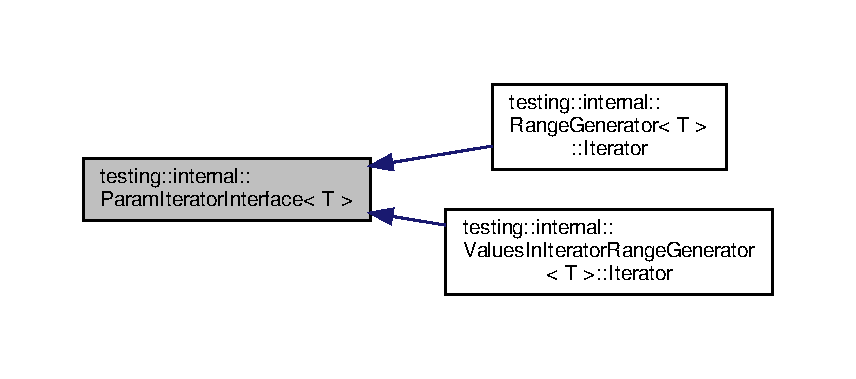
\includegraphics[width=350pt]{classtesting_1_1internal_1_1ParamIteratorInterface__inherit__graph}
\end{center}
\end{figure}
\subsection*{Public Member Functions}
\begin{DoxyCompactItemize}
\item 
virtual \hyperlink{classtesting_1_1internal_1_1ParamIteratorInterface_adf6ba49e6b54a6e3b15dbd5733988bef}{$\sim$\+Param\+Iterator\+Interface} ()
\item 
virtual const \hyperlink{classtesting_1_1internal_1_1ParamGeneratorInterface}{Param\+Generator\+Interface}$<$ T $>$ $\ast$ \hyperlink{classtesting_1_1internal_1_1ParamIteratorInterface_a17500953df75ecda1ace46c08ff731e9}{Base\+Generator} () const =0
\item 
virtual void \hyperlink{classtesting_1_1internal_1_1ParamIteratorInterface_a600dbd35fcb551463e379516a1abea48}{Advance} ()=0
\item 
virtual \hyperlink{classtesting_1_1internal_1_1ParamIteratorInterface}{Param\+Iterator\+Interface} $\ast$ \hyperlink{classtesting_1_1internal_1_1ParamIteratorInterface_a4998c23e27e2943d97546011aa35db80}{Clone} () const =0
\item 
virtual const T $\ast$ \hyperlink{classtesting_1_1internal_1_1ParamIteratorInterface_adfff808576d929085679c315b255af7e}{Current} () const =0
\item 
virtual bool \hyperlink{classtesting_1_1internal_1_1ParamIteratorInterface_a9d811697a752d46f7bd6a0082f9040a3}{Equals} (const \hyperlink{classtesting_1_1internal_1_1ParamIteratorInterface}{Param\+Iterator\+Interface} \&other) const =0
\end{DoxyCompactItemize}


\subsection{Constructor \& Destructor Documentation}
\mbox{\Hypertarget{classtesting_1_1internal_1_1ParamIteratorInterface_adf6ba49e6b54a6e3b15dbd5733988bef}\label{classtesting_1_1internal_1_1ParamIteratorInterface_adf6ba49e6b54a6e3b15dbd5733988bef}} 
\index{testing\+::internal\+::\+Param\+Iterator\+Interface@{testing\+::internal\+::\+Param\+Iterator\+Interface}!````~Param\+Iterator\+Interface@{$\sim$\+Param\+Iterator\+Interface}}
\index{````~Param\+Iterator\+Interface@{$\sim$\+Param\+Iterator\+Interface}!testing\+::internal\+::\+Param\+Iterator\+Interface@{testing\+::internal\+::\+Param\+Iterator\+Interface}}
\subsubsection{\texorpdfstring{$\sim$\+Param\+Iterator\+Interface()}{~ParamIteratorInterface()}}
{\footnotesize\ttfamily template$<$typename T$>$ \\
virtual \hyperlink{classtesting_1_1internal_1_1ParamIteratorInterface}{testing\+::internal\+::\+Param\+Iterator\+Interface}$<$ T $>$\+::$\sim$\hyperlink{classtesting_1_1internal_1_1ParamIteratorInterface}{Param\+Iterator\+Interface} (\begin{DoxyParamCaption}{ }\end{DoxyParamCaption})\hspace{0.3cm}{\ttfamily [inline]}, {\ttfamily [virtual]}}



\subsection{Member Function Documentation}
\mbox{\Hypertarget{classtesting_1_1internal_1_1ParamIteratorInterface_a600dbd35fcb551463e379516a1abea48}\label{classtesting_1_1internal_1_1ParamIteratorInterface_a600dbd35fcb551463e379516a1abea48}} 
\index{testing\+::internal\+::\+Param\+Iterator\+Interface@{testing\+::internal\+::\+Param\+Iterator\+Interface}!Advance@{Advance}}
\index{Advance@{Advance}!testing\+::internal\+::\+Param\+Iterator\+Interface@{testing\+::internal\+::\+Param\+Iterator\+Interface}}
\subsubsection{\texorpdfstring{Advance()}{Advance()}}
{\footnotesize\ttfamily template$<$typename T$>$ \\
virtual void \hyperlink{classtesting_1_1internal_1_1ParamIteratorInterface}{testing\+::internal\+::\+Param\+Iterator\+Interface}$<$ T $>$\+::Advance (\begin{DoxyParamCaption}{ }\end{DoxyParamCaption})\hspace{0.3cm}{\ttfamily [pure virtual]}}



Implemented in \hyperlink{classtesting_1_1internal_1_1CartesianProductGenerator_1_1IteratorImpl_3_01IndexSequence_3_01I_8_8_8_01_4_01_4_a167e8b38118c8635d5849daf924a517b}{testing\+::internal\+::\+Cartesian\+Product\+Generator$<$ T $>$\+::\+Iterator\+Impl$<$ Index\+Sequence$<$ I... $>$ $>$}, \hyperlink{classtesting_1_1internal_1_1ValuesInIteratorRangeGenerator_1_1Iterator_a5ff56489536cf5d90ed0ac07ffeb476b}{testing\+::internal\+::\+Values\+In\+Iterator\+Range\+Generator$<$ T $>$\+::\+Iterator}, and \hyperlink{classtesting_1_1internal_1_1RangeGenerator_1_1Iterator_ad17bd99e352c43b8ab654a4ad479d06e}{testing\+::internal\+::\+Range\+Generator$<$ T, Increment\+T $>$\+::\+Iterator}.

\mbox{\Hypertarget{classtesting_1_1internal_1_1ParamIteratorInterface_a17500953df75ecda1ace46c08ff731e9}\label{classtesting_1_1internal_1_1ParamIteratorInterface_a17500953df75ecda1ace46c08ff731e9}} 
\index{testing\+::internal\+::\+Param\+Iterator\+Interface@{testing\+::internal\+::\+Param\+Iterator\+Interface}!Base\+Generator@{Base\+Generator}}
\index{Base\+Generator@{Base\+Generator}!testing\+::internal\+::\+Param\+Iterator\+Interface@{testing\+::internal\+::\+Param\+Iterator\+Interface}}
\subsubsection{\texorpdfstring{Base\+Generator()}{BaseGenerator()}}
{\footnotesize\ttfamily template$<$typename T$>$ \\
virtual const \hyperlink{classtesting_1_1internal_1_1ParamGeneratorInterface}{Param\+Generator\+Interface}$<$T$>$$\ast$ \hyperlink{classtesting_1_1internal_1_1ParamIteratorInterface}{testing\+::internal\+::\+Param\+Iterator\+Interface}$<$ T $>$\+::Base\+Generator (\begin{DoxyParamCaption}{ }\end{DoxyParamCaption}) const\hspace{0.3cm}{\ttfamily [pure virtual]}}



Implemented in \hyperlink{classtesting_1_1internal_1_1CartesianProductGenerator_1_1IteratorImpl_3_01IndexSequence_3_01I_8_8_8_01_4_01_4_a8fa3ea322a1348fc8065481aba76e860}{testing\+::internal\+::\+Cartesian\+Product\+Generator$<$ T $>$\+::\+Iterator\+Impl$<$ Index\+Sequence$<$ I... $>$ $>$}, \hyperlink{classtesting_1_1internal_1_1ValuesInIteratorRangeGenerator_1_1Iterator_a27445e4d010ffde9d3f2f9ada5d54d0f}{testing\+::internal\+::\+Values\+In\+Iterator\+Range\+Generator$<$ T $>$\+::\+Iterator}, and \hyperlink{classtesting_1_1internal_1_1RangeGenerator_1_1Iterator_aa1dc4151e1eed1c546059ecb4f72440b}{testing\+::internal\+::\+Range\+Generator$<$ T, Increment\+T $>$\+::\+Iterator}.

\mbox{\Hypertarget{classtesting_1_1internal_1_1ParamIteratorInterface_a4998c23e27e2943d97546011aa35db80}\label{classtesting_1_1internal_1_1ParamIteratorInterface_a4998c23e27e2943d97546011aa35db80}} 
\index{testing\+::internal\+::\+Param\+Iterator\+Interface@{testing\+::internal\+::\+Param\+Iterator\+Interface}!Clone@{Clone}}
\index{Clone@{Clone}!testing\+::internal\+::\+Param\+Iterator\+Interface@{testing\+::internal\+::\+Param\+Iterator\+Interface}}
\subsubsection{\texorpdfstring{Clone()}{Clone()}}
{\footnotesize\ttfamily template$<$typename T$>$ \\
virtual \hyperlink{classtesting_1_1internal_1_1ParamIteratorInterface}{Param\+Iterator\+Interface}$\ast$ \hyperlink{classtesting_1_1internal_1_1ParamIteratorInterface}{testing\+::internal\+::\+Param\+Iterator\+Interface}$<$ T $>$\+::Clone (\begin{DoxyParamCaption}{ }\end{DoxyParamCaption}) const\hspace{0.3cm}{\ttfamily [pure virtual]}}



Implemented in \hyperlink{classtesting_1_1internal_1_1CartesianProductGenerator_1_1IteratorImpl_3_01IndexSequence_3_01I_8_8_8_01_4_01_4_a0b434e09b32dfd6b444085cf95dc22ab}{testing\+::internal\+::\+Cartesian\+Product\+Generator$<$ T $>$\+::\+Iterator\+Impl$<$ Index\+Sequence$<$ I... $>$ $>$}, \hyperlink{classtesting_1_1internal_1_1ValuesInIteratorRangeGenerator_1_1Iterator_a2c5ccf4da12cfb089829438d679ae35e}{testing\+::internal\+::\+Values\+In\+Iterator\+Range\+Generator$<$ T $>$\+::\+Iterator}, and \hyperlink{classtesting_1_1internal_1_1RangeGenerator_1_1Iterator_a61a764294b66272d730f5ff5e0acdcf4}{testing\+::internal\+::\+Range\+Generator$<$ T, Increment\+T $>$\+::\+Iterator}.

\mbox{\Hypertarget{classtesting_1_1internal_1_1ParamIteratorInterface_adfff808576d929085679c315b255af7e}\label{classtesting_1_1internal_1_1ParamIteratorInterface_adfff808576d929085679c315b255af7e}} 
\index{testing\+::internal\+::\+Param\+Iterator\+Interface@{testing\+::internal\+::\+Param\+Iterator\+Interface}!Current@{Current}}
\index{Current@{Current}!testing\+::internal\+::\+Param\+Iterator\+Interface@{testing\+::internal\+::\+Param\+Iterator\+Interface}}
\subsubsection{\texorpdfstring{Current()}{Current()}}
{\footnotesize\ttfamily template$<$typename T$>$ \\
virtual const T$\ast$ \hyperlink{classtesting_1_1internal_1_1ParamIteratorInterface}{testing\+::internal\+::\+Param\+Iterator\+Interface}$<$ T $>$\+::Current (\begin{DoxyParamCaption}{ }\end{DoxyParamCaption}) const\hspace{0.3cm}{\ttfamily [pure virtual]}}



Implemented in \hyperlink{classtesting_1_1internal_1_1CartesianProductGenerator_1_1IteratorImpl_3_01IndexSequence_3_01I_8_8_8_01_4_01_4_ab7052f320ab8ff3113a3e744a1bff07e}{testing\+::internal\+::\+Cartesian\+Product\+Generator$<$ T $>$\+::\+Iterator\+Impl$<$ Index\+Sequence$<$ I... $>$ $>$}, \hyperlink{classtesting_1_1internal_1_1ValuesInIteratorRangeGenerator_1_1Iterator_a55bd2a0d5a630478e32ec2efe08e37e4}{testing\+::internal\+::\+Values\+In\+Iterator\+Range\+Generator$<$ T $>$\+::\+Iterator}, and \hyperlink{classtesting_1_1internal_1_1RangeGenerator_1_1Iterator_acbdfc5919d37fb9514914afb041e50ff}{testing\+::internal\+::\+Range\+Generator$<$ T, Increment\+T $>$\+::\+Iterator}.

\mbox{\Hypertarget{classtesting_1_1internal_1_1ParamIteratorInterface_a9d811697a752d46f7bd6a0082f9040a3}\label{classtesting_1_1internal_1_1ParamIteratorInterface_a9d811697a752d46f7bd6a0082f9040a3}} 
\index{testing\+::internal\+::\+Param\+Iterator\+Interface@{testing\+::internal\+::\+Param\+Iterator\+Interface}!Equals@{Equals}}
\index{Equals@{Equals}!testing\+::internal\+::\+Param\+Iterator\+Interface@{testing\+::internal\+::\+Param\+Iterator\+Interface}}
\subsubsection{\texorpdfstring{Equals()}{Equals()}}
{\footnotesize\ttfamily template$<$typename T$>$ \\
virtual bool \hyperlink{classtesting_1_1internal_1_1ParamIteratorInterface}{testing\+::internal\+::\+Param\+Iterator\+Interface}$<$ T $>$\+::Equals (\begin{DoxyParamCaption}\item[{const \hyperlink{classtesting_1_1internal_1_1ParamIteratorInterface}{Param\+Iterator\+Interface}$<$ T $>$ \&}]{other }\end{DoxyParamCaption}) const\hspace{0.3cm}{\ttfamily [pure virtual]}}



Implemented in \hyperlink{classtesting_1_1internal_1_1ValuesInIteratorRangeGenerator_1_1Iterator_a75604bc318aca22ff8607b68bfb44e96}{testing\+::internal\+::\+Values\+In\+Iterator\+Range\+Generator$<$ T $>$\+::\+Iterator}, and \hyperlink{classtesting_1_1internal_1_1RangeGenerator_1_1Iterator_a534406abbddb137d7672c2b53d5bff0b}{testing\+::internal\+::\+Range\+Generator$<$ T, Increment\+T $>$\+::\+Iterator}.



The documentation for this class was generated from the following file\+:\begin{DoxyCompactItemize}
\item 
tests/googletest/include/gtest/internal/\hyperlink{gtest-param-util_8h}{gtest-\/param-\/util.\+h}\end{DoxyCompactItemize}

\hypertarget{classPreCalculatedPrimeTable}{}\section{Pre\+Calculated\+Prime\+Table Class Reference}
\label{classPreCalculatedPrimeTable}\index{Pre\+Calculated\+Prime\+Table@{Pre\+Calculated\+Prime\+Table}}


{\ttfamily \#include $<$prime\+\_\+tables.\+h$>$}



Inheritance diagram for Pre\+Calculated\+Prime\+Table\+:\nopagebreak
\begin{figure}[H]
\begin{center}
\leavevmode
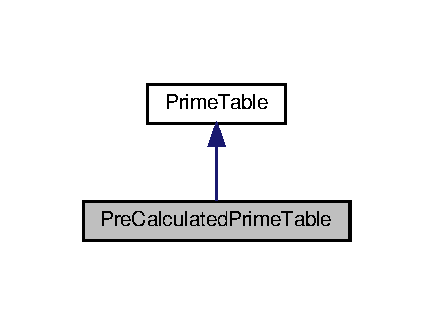
\includegraphics[width=208pt]{classPreCalculatedPrimeTable__inherit__graph}
\end{center}
\end{figure}


Collaboration diagram for Pre\+Calculated\+Prime\+Table\+:\nopagebreak
\begin{figure}[H]
\begin{center}
\leavevmode
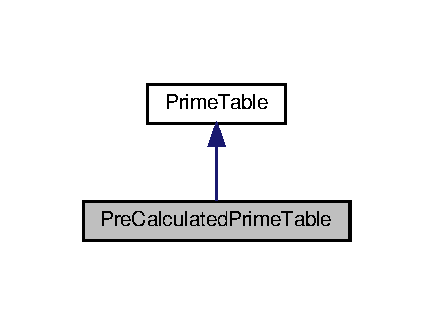
\includegraphics[width=208pt]{classPreCalculatedPrimeTable__coll__graph}
\end{center}
\end{figure}
\subsection*{Public Member Functions}
\begin{DoxyCompactItemize}
\item 
\hyperlink{classPreCalculatedPrimeTable_a6bb947504421e31da70d2c71576be350}{Pre\+Calculated\+Prime\+Table} (int max)
\item 
\hyperlink{classPreCalculatedPrimeTable_aeb9fb66a80367344b6ffe9c343b73464}{$\sim$\+Pre\+Calculated\+Prime\+Table} () override
\item 
bool \hyperlink{classPreCalculatedPrimeTable_a62be946777f7f98bbfc01edc0f15a4bb}{Is\+Prime} (int n) const override
\item 
int \hyperlink{classPreCalculatedPrimeTable_a0b99de0a790db9f0cc2b3cd4b527fd5a}{Get\+Next\+Prime} (int p) const override
\end{DoxyCompactItemize}
\subsection*{Private Member Functions}
\begin{DoxyCompactItemize}
\item 
void \hyperlink{classPreCalculatedPrimeTable_a393cb4947a57da9442e435eeff168b76}{Calculate\+Primes\+Up\+To} (int max)
\item 
void \hyperlink{classPreCalculatedPrimeTable_a67012c43b78cee27b891a9934becc455}{operator=} (const \hyperlink{classPreCalculatedPrimeTable}{Pre\+Calculated\+Prime\+Table} \&rhs)
\end{DoxyCompactItemize}
\subsection*{Private Attributes}
\begin{DoxyCompactItemize}
\item 
const int \hyperlink{classPreCalculatedPrimeTable_ad4275df41c5e5be3cad8c5abeaad1ac6}{is\+\_\+prime\+\_\+size\+\_\+}
\item 
bool $\ast$const \hyperlink{classPreCalculatedPrimeTable_ac393ebf41a32b3cba39fe67f7aa5fa38}{is\+\_\+prime\+\_\+}
\end{DoxyCompactItemize}


\subsection{Constructor \& Destructor Documentation}
\mbox{\Hypertarget{classPreCalculatedPrimeTable_a6bb947504421e31da70d2c71576be350}\label{classPreCalculatedPrimeTable_a6bb947504421e31da70d2c71576be350}} 
\index{Pre\+Calculated\+Prime\+Table@{Pre\+Calculated\+Prime\+Table}!Pre\+Calculated\+Prime\+Table@{Pre\+Calculated\+Prime\+Table}}
\index{Pre\+Calculated\+Prime\+Table@{Pre\+Calculated\+Prime\+Table}!Pre\+Calculated\+Prime\+Table@{Pre\+Calculated\+Prime\+Table}}
\subsubsection{\texorpdfstring{Pre\+Calculated\+Prime\+Table()}{PreCalculatedPrimeTable()}}
{\footnotesize\ttfamily Pre\+Calculated\+Prime\+Table\+::\+Pre\+Calculated\+Prime\+Table (\begin{DoxyParamCaption}\item[{int}]{max }\end{DoxyParamCaption})\hspace{0.3cm}{\ttfamily [inline]}, {\ttfamily [explicit]}}

\mbox{\Hypertarget{classPreCalculatedPrimeTable_aeb9fb66a80367344b6ffe9c343b73464}\label{classPreCalculatedPrimeTable_aeb9fb66a80367344b6ffe9c343b73464}} 
\index{Pre\+Calculated\+Prime\+Table@{Pre\+Calculated\+Prime\+Table}!````~Pre\+Calculated\+Prime\+Table@{$\sim$\+Pre\+Calculated\+Prime\+Table}}
\index{````~Pre\+Calculated\+Prime\+Table@{$\sim$\+Pre\+Calculated\+Prime\+Table}!Pre\+Calculated\+Prime\+Table@{Pre\+Calculated\+Prime\+Table}}
\subsubsection{\texorpdfstring{$\sim$\+Pre\+Calculated\+Prime\+Table()}{~PreCalculatedPrimeTable()}}
{\footnotesize\ttfamily Pre\+Calculated\+Prime\+Table\+::$\sim$\+Pre\+Calculated\+Prime\+Table (\begin{DoxyParamCaption}{ }\end{DoxyParamCaption})\hspace{0.3cm}{\ttfamily [inline]}, {\ttfamily [override]}}



\subsection{Member Function Documentation}
\mbox{\Hypertarget{classPreCalculatedPrimeTable_a393cb4947a57da9442e435eeff168b76}\label{classPreCalculatedPrimeTable_a393cb4947a57da9442e435eeff168b76}} 
\index{Pre\+Calculated\+Prime\+Table@{Pre\+Calculated\+Prime\+Table}!Calculate\+Primes\+Up\+To@{Calculate\+Primes\+Up\+To}}
\index{Calculate\+Primes\+Up\+To@{Calculate\+Primes\+Up\+To}!Pre\+Calculated\+Prime\+Table@{Pre\+Calculated\+Prime\+Table}}
\subsubsection{\texorpdfstring{Calculate\+Primes\+Up\+To()}{CalculatePrimesUpTo()}}
{\footnotesize\ttfamily void Pre\+Calculated\+Prime\+Table\+::\+Calculate\+Primes\+Up\+To (\begin{DoxyParamCaption}\item[{int}]{max }\end{DoxyParamCaption})\hspace{0.3cm}{\ttfamily [inline]}, {\ttfamily [private]}}

\mbox{\Hypertarget{classPreCalculatedPrimeTable_a0b99de0a790db9f0cc2b3cd4b527fd5a}\label{classPreCalculatedPrimeTable_a0b99de0a790db9f0cc2b3cd4b527fd5a}} 
\index{Pre\+Calculated\+Prime\+Table@{Pre\+Calculated\+Prime\+Table}!Get\+Next\+Prime@{Get\+Next\+Prime}}
\index{Get\+Next\+Prime@{Get\+Next\+Prime}!Pre\+Calculated\+Prime\+Table@{Pre\+Calculated\+Prime\+Table}}
\subsubsection{\texorpdfstring{Get\+Next\+Prime()}{GetNextPrime()}}
{\footnotesize\ttfamily int Pre\+Calculated\+Prime\+Table\+::\+Get\+Next\+Prime (\begin{DoxyParamCaption}\item[{int}]{p }\end{DoxyParamCaption}) const\hspace{0.3cm}{\ttfamily [inline]}, {\ttfamily [override]}, {\ttfamily [virtual]}}



Implements \hyperlink{classPrimeTable_ae537c939f56617d8937d57bbbae3ab30}{Prime\+Table}.

\mbox{\Hypertarget{classPreCalculatedPrimeTable_a62be946777f7f98bbfc01edc0f15a4bb}\label{classPreCalculatedPrimeTable_a62be946777f7f98bbfc01edc0f15a4bb}} 
\index{Pre\+Calculated\+Prime\+Table@{Pre\+Calculated\+Prime\+Table}!Is\+Prime@{Is\+Prime}}
\index{Is\+Prime@{Is\+Prime}!Pre\+Calculated\+Prime\+Table@{Pre\+Calculated\+Prime\+Table}}
\subsubsection{\texorpdfstring{Is\+Prime()}{IsPrime()}}
{\footnotesize\ttfamily bool Pre\+Calculated\+Prime\+Table\+::\+Is\+Prime (\begin{DoxyParamCaption}\item[{int}]{n }\end{DoxyParamCaption}) const\hspace{0.3cm}{\ttfamily [inline]}, {\ttfamily [override]}, {\ttfamily [virtual]}}



Implements \hyperlink{classPrimeTable_a2ab9243364ded0c51541f641b2df362a}{Prime\+Table}.

\mbox{\Hypertarget{classPreCalculatedPrimeTable_a67012c43b78cee27b891a9934becc455}\label{classPreCalculatedPrimeTable_a67012c43b78cee27b891a9934becc455}} 
\index{Pre\+Calculated\+Prime\+Table@{Pre\+Calculated\+Prime\+Table}!operator=@{operator=}}
\index{operator=@{operator=}!Pre\+Calculated\+Prime\+Table@{Pre\+Calculated\+Prime\+Table}}
\subsubsection{\texorpdfstring{operator=()}{operator=()}}
{\footnotesize\ttfamily void Pre\+Calculated\+Prime\+Table\+::operator= (\begin{DoxyParamCaption}\item[{const \hyperlink{classPreCalculatedPrimeTable}{Pre\+Calculated\+Prime\+Table} \&}]{rhs }\end{DoxyParamCaption})\hspace{0.3cm}{\ttfamily [private]}}



\subsection{Member Data Documentation}
\mbox{\Hypertarget{classPreCalculatedPrimeTable_ac393ebf41a32b3cba39fe67f7aa5fa38}\label{classPreCalculatedPrimeTable_ac393ebf41a32b3cba39fe67f7aa5fa38}} 
\index{Pre\+Calculated\+Prime\+Table@{Pre\+Calculated\+Prime\+Table}!is\+\_\+prime\+\_\+@{is\+\_\+prime\+\_\+}}
\index{is\+\_\+prime\+\_\+@{is\+\_\+prime\+\_\+}!Pre\+Calculated\+Prime\+Table@{Pre\+Calculated\+Prime\+Table}}
\subsubsection{\texorpdfstring{is\+\_\+prime\+\_\+}{is\_prime\_}}
{\footnotesize\ttfamily bool$\ast$ const Pre\+Calculated\+Prime\+Table\+::is\+\_\+prime\+\_\+\hspace{0.3cm}{\ttfamily [private]}}

\mbox{\Hypertarget{classPreCalculatedPrimeTable_ad4275df41c5e5be3cad8c5abeaad1ac6}\label{classPreCalculatedPrimeTable_ad4275df41c5e5be3cad8c5abeaad1ac6}} 
\index{Pre\+Calculated\+Prime\+Table@{Pre\+Calculated\+Prime\+Table}!is\+\_\+prime\+\_\+size\+\_\+@{is\+\_\+prime\+\_\+size\+\_\+}}
\index{is\+\_\+prime\+\_\+size\+\_\+@{is\+\_\+prime\+\_\+size\+\_\+}!Pre\+Calculated\+Prime\+Table@{Pre\+Calculated\+Prime\+Table}}
\subsubsection{\texorpdfstring{is\+\_\+prime\+\_\+size\+\_\+}{is\_prime\_size\_}}
{\footnotesize\ttfamily const int Pre\+Calculated\+Prime\+Table\+::is\+\_\+prime\+\_\+size\+\_\+\hspace{0.3cm}{\ttfamily [private]}}



The documentation for this class was generated from the following file\+:\begin{DoxyCompactItemize}
\item 
tests/googletest/samples/\hyperlink{prime__tables_8h}{prime\+\_\+tables.\+h}\end{DoxyCompactItemize}

\hypertarget{classPrimeTable}{}\section{Prime\+Table Class Reference}
\label{classPrimeTable}\index{Prime\+Table@{Prime\+Table}}


{\ttfamily \#include $<$prime\+\_\+tables.\+h$>$}



Inheritance diagram for Prime\+Table\+:\nopagebreak
\begin{figure}[H]
\begin{center}
\leavevmode
\includegraphics[width=336pt]{classPrimeTable__inherit__graph}
\end{center}
\end{figure}
\subsection*{Public Member Functions}
\begin{DoxyCompactItemize}
\item 
virtual \hyperlink{classPrimeTable_af2cdea4896fd86a42b4dfd5e5027d640}{$\sim$\+Prime\+Table} ()
\item 
virtual bool \hyperlink{classPrimeTable_a2ab9243364ded0c51541f641b2df362a}{Is\+Prime} (int n) const =0
\item 
virtual int \hyperlink{classPrimeTable_ae537c939f56617d8937d57bbbae3ab30}{Get\+Next\+Prime} (int p) const =0
\end{DoxyCompactItemize}


\subsection{Constructor \& Destructor Documentation}
\mbox{\Hypertarget{classPrimeTable_af2cdea4896fd86a42b4dfd5e5027d640}\label{classPrimeTable_af2cdea4896fd86a42b4dfd5e5027d640}} 
\index{Prime\+Table@{Prime\+Table}!````~Prime\+Table@{$\sim$\+Prime\+Table}}
\index{````~Prime\+Table@{$\sim$\+Prime\+Table}!Prime\+Table@{Prime\+Table}}
\subsubsection{\texorpdfstring{$\sim$\+Prime\+Table()}{~PrimeTable()}}
{\footnotesize\ttfamily virtual Prime\+Table\+::$\sim$\+Prime\+Table (\begin{DoxyParamCaption}{ }\end{DoxyParamCaption})\hspace{0.3cm}{\ttfamily [inline]}, {\ttfamily [virtual]}}



\subsection{Member Function Documentation}
\mbox{\Hypertarget{classPrimeTable_ae537c939f56617d8937d57bbbae3ab30}\label{classPrimeTable_ae537c939f56617d8937d57bbbae3ab30}} 
\index{Prime\+Table@{Prime\+Table}!Get\+Next\+Prime@{Get\+Next\+Prime}}
\index{Get\+Next\+Prime@{Get\+Next\+Prime}!Prime\+Table@{Prime\+Table}}
\subsubsection{\texorpdfstring{Get\+Next\+Prime()}{GetNextPrime()}}
{\footnotesize\ttfamily virtual int Prime\+Table\+::\+Get\+Next\+Prime (\begin{DoxyParamCaption}\item[{int}]{p }\end{DoxyParamCaption}) const\hspace{0.3cm}{\ttfamily [pure virtual]}}



Implemented in \hyperlink{classPreCalculatedPrimeTable_a0b99de0a790db9f0cc2b3cd4b527fd5a}{Pre\+Calculated\+Prime\+Table}, and \hyperlink{classOnTheFlyPrimeTable_a0f6f934f318407a812098e67584b60bf}{On\+The\+Fly\+Prime\+Table}.

\mbox{\Hypertarget{classPrimeTable_a2ab9243364ded0c51541f641b2df362a}\label{classPrimeTable_a2ab9243364ded0c51541f641b2df362a}} 
\index{Prime\+Table@{Prime\+Table}!Is\+Prime@{Is\+Prime}}
\index{Is\+Prime@{Is\+Prime}!Prime\+Table@{Prime\+Table}}
\subsubsection{\texorpdfstring{Is\+Prime()}{IsPrime()}}
{\footnotesize\ttfamily virtual bool Prime\+Table\+::\+Is\+Prime (\begin{DoxyParamCaption}\item[{int}]{n }\end{DoxyParamCaption}) const\hspace{0.3cm}{\ttfamily [pure virtual]}}



Implemented in \hyperlink{classPreCalculatedPrimeTable_a62be946777f7f98bbfc01edc0f15a4bb}{Pre\+Calculated\+Prime\+Table}, and \hyperlink{classOnTheFlyPrimeTable_ac8236514299e4558a5220c3e06f7f61a}{On\+The\+Fly\+Prime\+Table}.



The documentation for this class was generated from the following file\+:\begin{DoxyCompactItemize}
\item 
tests/googletest/samples/\hyperlink{prime__tables_8h}{prime\+\_\+tables.\+h}\end{DoxyCompactItemize}

\hypertarget{structtesting_1_1PrintToStringParamName}{}\section{testing\+:\+:Print\+To\+String\+Param\+Name Struct Reference}
\label{structtesting_1_1PrintToStringParamName}\index{testing\+::\+Print\+To\+String\+Param\+Name@{testing\+::\+Print\+To\+String\+Param\+Name}}


{\ttfamily \#include $<$gtest-\/param-\/util.\+h$>$}

\subsection*{Public Member Functions}
\begin{DoxyCompactItemize}
\item 
{\footnotesize template$<$class Param\+Type $>$ }\\std\+::string \hyperlink{structtesting_1_1PrintToStringParamName_a05b411cfb75dadb2c3c0355aee1dcf21}{operator()} (const \hyperlink{structtesting_1_1TestParamInfo}{Test\+Param\+Info}$<$ Param\+Type $>$ \&info) const
\end{DoxyCompactItemize}


\subsection{Member Function Documentation}
\mbox{\Hypertarget{structtesting_1_1PrintToStringParamName_a05b411cfb75dadb2c3c0355aee1dcf21}\label{structtesting_1_1PrintToStringParamName_a05b411cfb75dadb2c3c0355aee1dcf21}} 
\index{testing\+::\+Print\+To\+String\+Param\+Name@{testing\+::\+Print\+To\+String\+Param\+Name}!operator()@{operator()}}
\index{operator()@{operator()}!testing\+::\+Print\+To\+String\+Param\+Name@{testing\+::\+Print\+To\+String\+Param\+Name}}
\subsubsection{\texorpdfstring{operator()()}{operator()()}}
{\footnotesize\ttfamily template$<$class Param\+Type $>$ \\
std\+::string testing\+::\+Print\+To\+String\+Param\+Name\+::operator() (\begin{DoxyParamCaption}\item[{const \hyperlink{structtesting_1_1TestParamInfo}{Test\+Param\+Info}$<$ Param\+Type $>$ \&}]{info }\end{DoxyParamCaption}) const\hspace{0.3cm}{\ttfamily [inline]}}



The documentation for this struct was generated from the following file\+:\begin{DoxyCompactItemize}
\item 
tests/googletest/include/gtest/internal/\hyperlink{gtest-param-util_8h}{gtest-\/param-\/util.\+h}\end{DoxyCompactItemize}

\hypertarget{classPrivateCode}{}\section{Private\+Code Class Reference}
\label{classPrivateCode}\index{Private\+Code@{Private\+Code}}


{\ttfamily \#include $<$production.\+h$>$}

\subsection*{Public Member Functions}
\begin{DoxyCompactItemize}
\item 
\hyperlink{classPrivateCode_a9a74a333501232539ab1636f0928d8f2}{F\+R\+I\+E\+N\+D\+\_\+\+T\+E\+ST} (Private\+Code\+Test, Can\+Access\+Private\+Members)
\item 
\hyperlink{classPrivateCode_a29b6823300f68d78691476eeeaed8a7c}{F\+R\+I\+E\+N\+D\+\_\+\+T\+E\+ST} (Private\+Code\+Fixture\+Test, Can\+Access\+Private\+Members)
\item 
\hyperlink{classPrivateCode_affe538411a99919d24ef09dffe1bb3eb}{Private\+Code} ()
\item 
int \hyperlink{classPrivateCode_a247781246ce4d0c66563eaa39ba5aaa9}{x} () const
\end{DoxyCompactItemize}
\subsection*{Private Member Functions}
\begin{DoxyCompactItemize}
\item 
void \hyperlink{classPrivateCode_a8d8ac6564d6425ea793f85848bb21b39}{set\+\_\+x} (int an\+\_\+x)
\end{DoxyCompactItemize}
\subsection*{Private Attributes}
\begin{DoxyCompactItemize}
\item 
int \hyperlink{classPrivateCode_a3590a614d8c76fa34fa4cea6f340c37f}{x\+\_\+}
\end{DoxyCompactItemize}


\subsection{Constructor \& Destructor Documentation}
\mbox{\Hypertarget{classPrivateCode_affe538411a99919d24ef09dffe1bb3eb}\label{classPrivateCode_affe538411a99919d24ef09dffe1bb3eb}} 
\index{Private\+Code@{Private\+Code}!Private\+Code@{Private\+Code}}
\index{Private\+Code@{Private\+Code}!Private\+Code@{Private\+Code}}
\subsubsection{\texorpdfstring{Private\+Code()}{PrivateCode()}}
{\footnotesize\ttfamily Private\+Code\+::\+Private\+Code (\begin{DoxyParamCaption}{ }\end{DoxyParamCaption})}



\subsection{Member Function Documentation}
\mbox{\Hypertarget{classPrivateCode_a9a74a333501232539ab1636f0928d8f2}\label{classPrivateCode_a9a74a333501232539ab1636f0928d8f2}} 
\index{Private\+Code@{Private\+Code}!F\+R\+I\+E\+N\+D\+\_\+\+T\+E\+ST@{F\+R\+I\+E\+N\+D\+\_\+\+T\+E\+ST}}
\index{F\+R\+I\+E\+N\+D\+\_\+\+T\+E\+ST@{F\+R\+I\+E\+N\+D\+\_\+\+T\+E\+ST}!Private\+Code@{Private\+Code}}
\subsubsection{\texorpdfstring{F\+R\+I\+E\+N\+D\+\_\+\+T\+E\+S\+T()}{FRIEND\_TEST()}\hspace{0.1cm}{\footnotesize\ttfamily [1/2]}}
{\footnotesize\ttfamily Private\+Code\+::\+F\+R\+I\+E\+N\+D\+\_\+\+T\+E\+ST (\begin{DoxyParamCaption}\item[{Private\+Code\+Test}]{,  }\item[{Can\+Access\+Private\+Members}]{ }\end{DoxyParamCaption})}

\mbox{\Hypertarget{classPrivateCode_a29b6823300f68d78691476eeeaed8a7c}\label{classPrivateCode_a29b6823300f68d78691476eeeaed8a7c}} 
\index{Private\+Code@{Private\+Code}!F\+R\+I\+E\+N\+D\+\_\+\+T\+E\+ST@{F\+R\+I\+E\+N\+D\+\_\+\+T\+E\+ST}}
\index{F\+R\+I\+E\+N\+D\+\_\+\+T\+E\+ST@{F\+R\+I\+E\+N\+D\+\_\+\+T\+E\+ST}!Private\+Code@{Private\+Code}}
\subsubsection{\texorpdfstring{F\+R\+I\+E\+N\+D\+\_\+\+T\+E\+S\+T()}{FRIEND\_TEST()}\hspace{0.1cm}{\footnotesize\ttfamily [2/2]}}
{\footnotesize\ttfamily Private\+Code\+::\+F\+R\+I\+E\+N\+D\+\_\+\+T\+E\+ST (\begin{DoxyParamCaption}\item[{Private\+Code\+Fixture\+Test}]{,  }\item[{Can\+Access\+Private\+Members}]{ }\end{DoxyParamCaption})}

\mbox{\Hypertarget{classPrivateCode_a8d8ac6564d6425ea793f85848bb21b39}\label{classPrivateCode_a8d8ac6564d6425ea793f85848bb21b39}} 
\index{Private\+Code@{Private\+Code}!set\+\_\+x@{set\+\_\+x}}
\index{set\+\_\+x@{set\+\_\+x}!Private\+Code@{Private\+Code}}
\subsubsection{\texorpdfstring{set\+\_\+x()}{set\_x()}}
{\footnotesize\ttfamily void Private\+Code\+::set\+\_\+x (\begin{DoxyParamCaption}\item[{int}]{an\+\_\+x }\end{DoxyParamCaption})\hspace{0.3cm}{\ttfamily [inline]}, {\ttfamily [private]}}

\mbox{\Hypertarget{classPrivateCode_a247781246ce4d0c66563eaa39ba5aaa9}\label{classPrivateCode_a247781246ce4d0c66563eaa39ba5aaa9}} 
\index{Private\+Code@{Private\+Code}!x@{x}}
\index{x@{x}!Private\+Code@{Private\+Code}}
\subsubsection{\texorpdfstring{x()}{x()}}
{\footnotesize\ttfamily int Private\+Code\+::x (\begin{DoxyParamCaption}{ }\end{DoxyParamCaption}) const\hspace{0.3cm}{\ttfamily [inline]}}



\subsection{Member Data Documentation}
\mbox{\Hypertarget{classPrivateCode_a3590a614d8c76fa34fa4cea6f340c37f}\label{classPrivateCode_a3590a614d8c76fa34fa4cea6f340c37f}} 
\index{Private\+Code@{Private\+Code}!x\+\_\+@{x\+\_\+}}
\index{x\+\_\+@{x\+\_\+}!Private\+Code@{Private\+Code}}
\subsubsection{\texorpdfstring{x\+\_\+}{x\_}}
{\footnotesize\ttfamily int Private\+Code\+::x\+\_\+\hspace{0.3cm}{\ttfamily [private]}}



The documentation for this class was generated from the following file\+:\begin{DoxyCompactItemize}
\item 
tests/googletest/test/\hyperlink{production_8h}{production.\+h}\end{DoxyCompactItemize}

\hypertarget{classQueue}{}\section{Queue$<$ E $>$ Class Template Reference}
\label{classQueue}\index{Queue$<$ E $>$@{Queue$<$ E $>$}}


{\ttfamily \#include $<$sample3-\/inl.\+h$>$}

\subsection*{Public Member Functions}
\begin{DoxyCompactItemize}
\item 
\hyperlink{classQueue_ab09891e54b51dc677ee6efb350687ae4}{Queue} ()
\item 
\hyperlink{classQueue_a49fe82adb8dc2fb62ab53876a6933d0f}{$\sim$\+Queue} ()
\item 
void \hyperlink{classQueue_acfdd5f9f7e936ca30dcf877370ef9510}{Clear} ()
\item 
size\+\_\+t \hyperlink{classQueue_abc4d78b5f66041011c5590bf703847b0}{Size} () const
\item 
\hyperlink{classQueueNode}{Queue\+Node}$<$ E $>$ $\ast$ \hyperlink{classQueue_a71aa0154ef75bb87a53b6af1829fcd5e}{Head} ()
\item 
const \hyperlink{classQueueNode}{Queue\+Node}$<$ E $>$ $\ast$ \hyperlink{classQueue_a6c906075e0ad2d1f0634990aa106395e}{Head} () const
\item 
\hyperlink{classQueueNode}{Queue\+Node}$<$ E $>$ $\ast$ \hyperlink{classQueue_a430aca3d3b9f5fd588b215028d134b74}{Last} ()
\item 
const \hyperlink{classQueueNode}{Queue\+Node}$<$ E $>$ $\ast$ \hyperlink{classQueue_a7c8c2c64700dfe1df8bf266572cf101a}{Last} () const
\item 
void \hyperlink{classQueue_abaa2e7175457307bca74f5562cbdaaa9}{Enqueue} (const E \&element)
\item 
E $\ast$ \hyperlink{classQueue_a434d465001c3078e999f7a89a8af84c0}{Dequeue} ()
\item 
{\footnotesize template$<$typename F $>$ }\\\hyperlink{classQueue}{Queue} $\ast$ \hyperlink{classQueue_a904a696292fc593adc6fd21fb229d760}{Map} (F function) const
\end{DoxyCompactItemize}
\subsection*{Private Member Functions}
\begin{DoxyCompactItemize}
\item 
\hyperlink{classQueue_ac071ee553005a67737d35edeeaafca5b}{Queue} (const \hyperlink{classQueue}{Queue} \&)
\item 
const \hyperlink{classQueue}{Queue} \& \hyperlink{classQueue_adf6f3eb046365f1b67b6c0bd5da2da59}{operator=} (const \hyperlink{classQueue}{Queue} \&)
\end{DoxyCompactItemize}
\subsection*{Private Attributes}
\begin{DoxyCompactItemize}
\item 
\hyperlink{classQueueNode}{Queue\+Node}$<$ E $>$ $\ast$ \hyperlink{classQueue_abf9219bcea800d26e8bfdb4777d98729}{head\+\_\+}
\item 
\hyperlink{classQueueNode}{Queue\+Node}$<$ E $>$ $\ast$ \hyperlink{classQueue_a7466dca4f96147c9124af582ab170df0}{last\+\_\+}
\item 
size\+\_\+t \hyperlink{classQueue_a7ac3c0717d894e1aecc56f4ddb35c7ea}{size\+\_\+}
\end{DoxyCompactItemize}


\subsection{Constructor \& Destructor Documentation}
\mbox{\Hypertarget{classQueue_ab09891e54b51dc677ee6efb350687ae4}\label{classQueue_ab09891e54b51dc677ee6efb350687ae4}} 
\index{Queue@{Queue}!Queue@{Queue}}
\index{Queue@{Queue}!Queue@{Queue}}
\subsubsection{\texorpdfstring{Queue()}{Queue()}\hspace{0.1cm}{\footnotesize\ttfamily [1/2]}}
{\footnotesize\ttfamily template$<$typename E $>$ \\
\hyperlink{classQueue}{Queue}$<$ E $>$\+::\hyperlink{classQueue}{Queue} (\begin{DoxyParamCaption}{ }\end{DoxyParamCaption})\hspace{0.3cm}{\ttfamily [inline]}}

\mbox{\Hypertarget{classQueue_a49fe82adb8dc2fb62ab53876a6933d0f}\label{classQueue_a49fe82adb8dc2fb62ab53876a6933d0f}} 
\index{Queue@{Queue}!````~Queue@{$\sim$\+Queue}}
\index{````~Queue@{$\sim$\+Queue}!Queue@{Queue}}
\subsubsection{\texorpdfstring{$\sim$\+Queue()}{~Queue()}}
{\footnotesize\ttfamily template$<$typename E $>$ \\
\hyperlink{classQueue}{Queue}$<$ E $>$\+::$\sim$\hyperlink{classQueue}{Queue} (\begin{DoxyParamCaption}{ }\end{DoxyParamCaption})\hspace{0.3cm}{\ttfamily [inline]}}

\mbox{\Hypertarget{classQueue_ac071ee553005a67737d35edeeaafca5b}\label{classQueue_ac071ee553005a67737d35edeeaafca5b}} 
\index{Queue@{Queue}!Queue@{Queue}}
\index{Queue@{Queue}!Queue@{Queue}}
\subsubsection{\texorpdfstring{Queue()}{Queue()}\hspace{0.1cm}{\footnotesize\ttfamily [2/2]}}
{\footnotesize\ttfamily template$<$typename E $>$ \\
\hyperlink{classQueue}{Queue}$<$ E $>$\+::\hyperlink{classQueue}{Queue} (\begin{DoxyParamCaption}\item[{const \hyperlink{classQueue}{Queue}$<$ E $>$ \&}]{ }\end{DoxyParamCaption})\hspace{0.3cm}{\ttfamily [private]}}



\subsection{Member Function Documentation}
\mbox{\Hypertarget{classQueue_acfdd5f9f7e936ca30dcf877370ef9510}\label{classQueue_acfdd5f9f7e936ca30dcf877370ef9510}} 
\index{Queue@{Queue}!Clear@{Clear}}
\index{Clear@{Clear}!Queue@{Queue}}
\subsubsection{\texorpdfstring{Clear()}{Clear()}}
{\footnotesize\ttfamily template$<$typename E $>$ \\
void \hyperlink{classQueue}{Queue}$<$ E $>$\+::Clear (\begin{DoxyParamCaption}{ }\end{DoxyParamCaption})\hspace{0.3cm}{\ttfamily [inline]}}

\mbox{\Hypertarget{classQueue_a434d465001c3078e999f7a89a8af84c0}\label{classQueue_a434d465001c3078e999f7a89a8af84c0}} 
\index{Queue@{Queue}!Dequeue@{Dequeue}}
\index{Dequeue@{Dequeue}!Queue@{Queue}}
\subsubsection{\texorpdfstring{Dequeue()}{Dequeue()}}
{\footnotesize\ttfamily template$<$typename E $>$ \\
E$\ast$ \hyperlink{classQueue}{Queue}$<$ E $>$\+::Dequeue (\begin{DoxyParamCaption}{ }\end{DoxyParamCaption})\hspace{0.3cm}{\ttfamily [inline]}}

\mbox{\Hypertarget{classQueue_abaa2e7175457307bca74f5562cbdaaa9}\label{classQueue_abaa2e7175457307bca74f5562cbdaaa9}} 
\index{Queue@{Queue}!Enqueue@{Enqueue}}
\index{Enqueue@{Enqueue}!Queue@{Queue}}
\subsubsection{\texorpdfstring{Enqueue()}{Enqueue()}}
{\footnotesize\ttfamily template$<$typename E $>$ \\
void \hyperlink{classQueue}{Queue}$<$ E $>$\+::Enqueue (\begin{DoxyParamCaption}\item[{const E \&}]{element }\end{DoxyParamCaption})\hspace{0.3cm}{\ttfamily [inline]}}

\mbox{\Hypertarget{classQueue_a71aa0154ef75bb87a53b6af1829fcd5e}\label{classQueue_a71aa0154ef75bb87a53b6af1829fcd5e}} 
\index{Queue@{Queue}!Head@{Head}}
\index{Head@{Head}!Queue@{Queue}}
\subsubsection{\texorpdfstring{Head()}{Head()}\hspace{0.1cm}{\footnotesize\ttfamily [1/2]}}
{\footnotesize\ttfamily template$<$typename E $>$ \\
\hyperlink{classQueueNode}{Queue\+Node}$<$E$>$$\ast$ \hyperlink{classQueue}{Queue}$<$ E $>$\+::Head (\begin{DoxyParamCaption}{ }\end{DoxyParamCaption})\hspace{0.3cm}{\ttfamily [inline]}}

\mbox{\Hypertarget{classQueue_a6c906075e0ad2d1f0634990aa106395e}\label{classQueue_a6c906075e0ad2d1f0634990aa106395e}} 
\index{Queue@{Queue}!Head@{Head}}
\index{Head@{Head}!Queue@{Queue}}
\subsubsection{\texorpdfstring{Head()}{Head()}\hspace{0.1cm}{\footnotesize\ttfamily [2/2]}}
{\footnotesize\ttfamily template$<$typename E $>$ \\
const \hyperlink{classQueueNode}{Queue\+Node}$<$E$>$$\ast$ \hyperlink{classQueue}{Queue}$<$ E $>$\+::Head (\begin{DoxyParamCaption}{ }\end{DoxyParamCaption}) const\hspace{0.3cm}{\ttfamily [inline]}}

\mbox{\Hypertarget{classQueue_a430aca3d3b9f5fd588b215028d134b74}\label{classQueue_a430aca3d3b9f5fd588b215028d134b74}} 
\index{Queue@{Queue}!Last@{Last}}
\index{Last@{Last}!Queue@{Queue}}
\subsubsection{\texorpdfstring{Last()}{Last()}\hspace{0.1cm}{\footnotesize\ttfamily [1/2]}}
{\footnotesize\ttfamily template$<$typename E $>$ \\
\hyperlink{classQueueNode}{Queue\+Node}$<$E$>$$\ast$ \hyperlink{classQueue}{Queue}$<$ E $>$\+::Last (\begin{DoxyParamCaption}{ }\end{DoxyParamCaption})\hspace{0.3cm}{\ttfamily [inline]}}

\mbox{\Hypertarget{classQueue_a7c8c2c64700dfe1df8bf266572cf101a}\label{classQueue_a7c8c2c64700dfe1df8bf266572cf101a}} 
\index{Queue@{Queue}!Last@{Last}}
\index{Last@{Last}!Queue@{Queue}}
\subsubsection{\texorpdfstring{Last()}{Last()}\hspace{0.1cm}{\footnotesize\ttfamily [2/2]}}
{\footnotesize\ttfamily template$<$typename E $>$ \\
const \hyperlink{classQueueNode}{Queue\+Node}$<$E$>$$\ast$ \hyperlink{classQueue}{Queue}$<$ E $>$\+::Last (\begin{DoxyParamCaption}{ }\end{DoxyParamCaption}) const\hspace{0.3cm}{\ttfamily [inline]}}

\mbox{\Hypertarget{classQueue_a904a696292fc593adc6fd21fb229d760}\label{classQueue_a904a696292fc593adc6fd21fb229d760}} 
\index{Queue@{Queue}!Map@{Map}}
\index{Map@{Map}!Queue@{Queue}}
\subsubsection{\texorpdfstring{Map()}{Map()}}
{\footnotesize\ttfamily template$<$typename E $>$ \\
template$<$typename F $>$ \\
\hyperlink{classQueue}{Queue}$\ast$ \hyperlink{classQueue}{Queue}$<$ E $>$\+::Map (\begin{DoxyParamCaption}\item[{F}]{function }\end{DoxyParamCaption}) const\hspace{0.3cm}{\ttfamily [inline]}}

\mbox{\Hypertarget{classQueue_adf6f3eb046365f1b67b6c0bd5da2da59}\label{classQueue_adf6f3eb046365f1b67b6c0bd5da2da59}} 
\index{Queue@{Queue}!operator=@{operator=}}
\index{operator=@{operator=}!Queue@{Queue}}
\subsubsection{\texorpdfstring{operator=()}{operator=()}}
{\footnotesize\ttfamily template$<$typename E $>$ \\
const \hyperlink{classQueue}{Queue}\& \hyperlink{classQueue}{Queue}$<$ E $>$\+::operator= (\begin{DoxyParamCaption}\item[{const \hyperlink{classQueue}{Queue}$<$ E $>$ \&}]{ }\end{DoxyParamCaption})\hspace{0.3cm}{\ttfamily [private]}}

\mbox{\Hypertarget{classQueue_abc4d78b5f66041011c5590bf703847b0}\label{classQueue_abc4d78b5f66041011c5590bf703847b0}} 
\index{Queue@{Queue}!Size@{Size}}
\index{Size@{Size}!Queue@{Queue}}
\subsubsection{\texorpdfstring{Size()}{Size()}}
{\footnotesize\ttfamily template$<$typename E $>$ \\
size\+\_\+t \hyperlink{classQueue}{Queue}$<$ E $>$\+::Size (\begin{DoxyParamCaption}{ }\end{DoxyParamCaption}) const\hspace{0.3cm}{\ttfamily [inline]}}



\subsection{Member Data Documentation}
\mbox{\Hypertarget{classQueue_abf9219bcea800d26e8bfdb4777d98729}\label{classQueue_abf9219bcea800d26e8bfdb4777d98729}} 
\index{Queue@{Queue}!head\+\_\+@{head\+\_\+}}
\index{head\+\_\+@{head\+\_\+}!Queue@{Queue}}
\subsubsection{\texorpdfstring{head\+\_\+}{head\_}}
{\footnotesize\ttfamily template$<$typename E $>$ \\
\hyperlink{classQueueNode}{Queue\+Node}$<$E$>$$\ast$ \hyperlink{classQueue}{Queue}$<$ E $>$\+::head\+\_\+\hspace{0.3cm}{\ttfamily [private]}}

\mbox{\Hypertarget{classQueue_a7466dca4f96147c9124af582ab170df0}\label{classQueue_a7466dca4f96147c9124af582ab170df0}} 
\index{Queue@{Queue}!last\+\_\+@{last\+\_\+}}
\index{last\+\_\+@{last\+\_\+}!Queue@{Queue}}
\subsubsection{\texorpdfstring{last\+\_\+}{last\_}}
{\footnotesize\ttfamily template$<$typename E $>$ \\
\hyperlink{classQueueNode}{Queue\+Node}$<$E$>$$\ast$ \hyperlink{classQueue}{Queue}$<$ E $>$\+::last\+\_\+\hspace{0.3cm}{\ttfamily [private]}}

\mbox{\Hypertarget{classQueue_a7ac3c0717d894e1aecc56f4ddb35c7ea}\label{classQueue_a7ac3c0717d894e1aecc56f4ddb35c7ea}} 
\index{Queue@{Queue}!size\+\_\+@{size\+\_\+}}
\index{size\+\_\+@{size\+\_\+}!Queue@{Queue}}
\subsubsection{\texorpdfstring{size\+\_\+}{size\_}}
{\footnotesize\ttfamily template$<$typename E $>$ \\
size\+\_\+t \hyperlink{classQueue}{Queue}$<$ E $>$\+::size\+\_\+\hspace{0.3cm}{\ttfamily [private]}}



The documentation for this class was generated from the following file\+:\begin{DoxyCompactItemize}
\item 
tests/googletest/samples/\hyperlink{sample3-inl_8h}{sample3-\/inl.\+h}\end{DoxyCompactItemize}

\hypertarget{classQueueNode}{}\section{Queue\+Node$<$ E $>$ Class Template Reference}
\label{classQueueNode}\index{Queue\+Node$<$ E $>$@{Queue\+Node$<$ E $>$}}


{\ttfamily \#include $<$sample3-\/inl.\+h$>$}



Collaboration diagram for Queue\+Node$<$ E $>$\+:\nopagebreak
\begin{figure}[H]
\begin{center}
\leavevmode
\includegraphics[width=219pt]{classQueueNode__coll__graph}
\end{center}
\end{figure}
\subsection*{Public Member Functions}
\begin{DoxyCompactItemize}
\item 
const E \& \hyperlink{classQueueNode_a1c61b3ed32e089f5901b87022ef84985}{element} () const
\item 
\hyperlink{classQueueNode}{Queue\+Node} $\ast$ \hyperlink{classQueueNode_a8a9fdf488da06533360999ef85db56ea}{next} ()
\item 
const \hyperlink{classQueueNode}{Queue\+Node} $\ast$ \hyperlink{classQueueNode_ada477e4f309f29383112dbda473dd985}{next} () const
\end{DoxyCompactItemize}
\subsection*{Private Member Functions}
\begin{DoxyCompactItemize}
\item 
\hyperlink{classQueueNode_a2c22feef35d910bec7138598e8784e25}{Queue\+Node} (const E \&an\+\_\+element)
\item 
const \hyperlink{classQueueNode}{Queue\+Node} \& \hyperlink{classQueueNode_a8635bbe6310e011ef4fcf1a01566dbb7}{operator=} (const \hyperlink{classQueueNode}{Queue\+Node} \&)
\item 
\hyperlink{classQueueNode_a35adcad7a84db46784907cf58106d585}{Queue\+Node} (const \hyperlink{classQueueNode}{Queue\+Node} \&)
\end{DoxyCompactItemize}
\subsection*{Private Attributes}
\begin{DoxyCompactItemize}
\item 
E \hyperlink{classQueueNode_a593f0f5862848c1e9063d32ea3438b58}{element\+\_\+}
\item 
\hyperlink{classQueueNode}{Queue\+Node} $\ast$ \hyperlink{classQueueNode_a7434603f6c25418f7810f041752876bd}{next\+\_\+}
\end{DoxyCompactItemize}
\subsection*{Friends}
\begin{DoxyCompactItemize}
\item 
class \hyperlink{classQueueNode_ad4336229b1d7c3626e4ba69f236b202d}{Queue$<$ E $>$}
\end{DoxyCompactItemize}


\subsection{Constructor \& Destructor Documentation}
\mbox{\Hypertarget{classQueueNode_a2c22feef35d910bec7138598e8784e25}\label{classQueueNode_a2c22feef35d910bec7138598e8784e25}} 
\index{Queue\+Node@{Queue\+Node}!Queue\+Node@{Queue\+Node}}
\index{Queue\+Node@{Queue\+Node}!Queue\+Node@{Queue\+Node}}
\subsubsection{\texorpdfstring{Queue\+Node()}{QueueNode()}\hspace{0.1cm}{\footnotesize\ttfamily [1/2]}}
{\footnotesize\ttfamily template$<$typename E$>$ \\
\hyperlink{classQueueNode}{Queue\+Node}$<$ E $>$\+::\hyperlink{classQueueNode}{Queue\+Node} (\begin{DoxyParamCaption}\item[{const E \&}]{an\+\_\+element }\end{DoxyParamCaption})\hspace{0.3cm}{\ttfamily [inline]}, {\ttfamily [explicit]}, {\ttfamily [private]}}

\mbox{\Hypertarget{classQueueNode_a35adcad7a84db46784907cf58106d585}\label{classQueueNode_a35adcad7a84db46784907cf58106d585}} 
\index{Queue\+Node@{Queue\+Node}!Queue\+Node@{Queue\+Node}}
\index{Queue\+Node@{Queue\+Node}!Queue\+Node@{Queue\+Node}}
\subsubsection{\texorpdfstring{Queue\+Node()}{QueueNode()}\hspace{0.1cm}{\footnotesize\ttfamily [2/2]}}
{\footnotesize\ttfamily template$<$typename E$>$ \\
\hyperlink{classQueueNode}{Queue\+Node}$<$ E $>$\+::\hyperlink{classQueueNode}{Queue\+Node} (\begin{DoxyParamCaption}\item[{const \hyperlink{classQueueNode}{Queue\+Node}$<$ E $>$ \&}]{ }\end{DoxyParamCaption})\hspace{0.3cm}{\ttfamily [private]}}



\subsection{Member Function Documentation}
\mbox{\Hypertarget{classQueueNode_a1c61b3ed32e089f5901b87022ef84985}\label{classQueueNode_a1c61b3ed32e089f5901b87022ef84985}} 
\index{Queue\+Node@{Queue\+Node}!element@{element}}
\index{element@{element}!Queue\+Node@{Queue\+Node}}
\subsubsection{\texorpdfstring{element()}{element()}}
{\footnotesize\ttfamily template$<$typename E$>$ \\
const E\& \hyperlink{classQueueNode}{Queue\+Node}$<$ E $>$\+::element (\begin{DoxyParamCaption}{ }\end{DoxyParamCaption}) const\hspace{0.3cm}{\ttfamily [inline]}}

\mbox{\Hypertarget{classQueueNode_a8a9fdf488da06533360999ef85db56ea}\label{classQueueNode_a8a9fdf488da06533360999ef85db56ea}} 
\index{Queue\+Node@{Queue\+Node}!next@{next}}
\index{next@{next}!Queue\+Node@{Queue\+Node}}
\subsubsection{\texorpdfstring{next()}{next()}\hspace{0.1cm}{\footnotesize\ttfamily [1/2]}}
{\footnotesize\ttfamily template$<$typename E$>$ \\
\hyperlink{classQueueNode}{Queue\+Node}$\ast$ \hyperlink{classQueueNode}{Queue\+Node}$<$ E $>$\+::next (\begin{DoxyParamCaption}{ }\end{DoxyParamCaption})\hspace{0.3cm}{\ttfamily [inline]}}

\mbox{\Hypertarget{classQueueNode_ada477e4f309f29383112dbda473dd985}\label{classQueueNode_ada477e4f309f29383112dbda473dd985}} 
\index{Queue\+Node@{Queue\+Node}!next@{next}}
\index{next@{next}!Queue\+Node@{Queue\+Node}}
\subsubsection{\texorpdfstring{next()}{next()}\hspace{0.1cm}{\footnotesize\ttfamily [2/2]}}
{\footnotesize\ttfamily template$<$typename E$>$ \\
const \hyperlink{classQueueNode}{Queue\+Node}$\ast$ \hyperlink{classQueueNode}{Queue\+Node}$<$ E $>$\+::next (\begin{DoxyParamCaption}{ }\end{DoxyParamCaption}) const\hspace{0.3cm}{\ttfamily [inline]}}

\mbox{\Hypertarget{classQueueNode_a8635bbe6310e011ef4fcf1a01566dbb7}\label{classQueueNode_a8635bbe6310e011ef4fcf1a01566dbb7}} 
\index{Queue\+Node@{Queue\+Node}!operator=@{operator=}}
\index{operator=@{operator=}!Queue\+Node@{Queue\+Node}}
\subsubsection{\texorpdfstring{operator=()}{operator=()}}
{\footnotesize\ttfamily template$<$typename E$>$ \\
const \hyperlink{classQueueNode}{Queue\+Node}\& \hyperlink{classQueueNode}{Queue\+Node}$<$ E $>$\+::operator= (\begin{DoxyParamCaption}\item[{const \hyperlink{classQueueNode}{Queue\+Node}$<$ E $>$ \&}]{ }\end{DoxyParamCaption})\hspace{0.3cm}{\ttfamily [private]}}



\subsection{Friends And Related Function Documentation}
\mbox{\Hypertarget{classQueueNode_ad4336229b1d7c3626e4ba69f236b202d}\label{classQueueNode_ad4336229b1d7c3626e4ba69f236b202d}} 
\index{Queue\+Node@{Queue\+Node}!Queue$<$ E $>$@{Queue$<$ E $>$}}
\index{Queue$<$ E $>$@{Queue$<$ E $>$}!Queue\+Node@{Queue\+Node}}
\subsubsection{\texorpdfstring{Queue$<$ E $>$}{Queue< E >}}
{\footnotesize\ttfamily template$<$typename E$>$ \\
friend class \hyperlink{classQueue}{Queue}$<$ E $>$\hspace{0.3cm}{\ttfamily [friend]}}



\subsection{Member Data Documentation}
\mbox{\Hypertarget{classQueueNode_a593f0f5862848c1e9063d32ea3438b58}\label{classQueueNode_a593f0f5862848c1e9063d32ea3438b58}} 
\index{Queue\+Node@{Queue\+Node}!element\+\_\+@{element\+\_\+}}
\index{element\+\_\+@{element\+\_\+}!Queue\+Node@{Queue\+Node}}
\subsubsection{\texorpdfstring{element\+\_\+}{element\_}}
{\footnotesize\ttfamily template$<$typename E$>$ \\
E \hyperlink{classQueueNode}{Queue\+Node}$<$ E $>$\+::element\+\_\+\hspace{0.3cm}{\ttfamily [private]}}

\mbox{\Hypertarget{classQueueNode_a7434603f6c25418f7810f041752876bd}\label{classQueueNode_a7434603f6c25418f7810f041752876bd}} 
\index{Queue\+Node@{Queue\+Node}!next\+\_\+@{next\+\_\+}}
\index{next\+\_\+@{next\+\_\+}!Queue\+Node@{Queue\+Node}}
\subsubsection{\texorpdfstring{next\+\_\+}{next\_}}
{\footnotesize\ttfamily template$<$typename E$>$ \\
\hyperlink{classQueueNode}{Queue\+Node}$\ast$ \hyperlink{classQueueNode}{Queue\+Node}$<$ E $>$\+::next\+\_\+\hspace{0.3cm}{\ttfamily [private]}}



The documentation for this class was generated from the following file\+:\begin{DoxyCompactItemize}
\item 
tests/googletest/samples/\hyperlink{sample3-inl_8h}{sample3-\/inl.\+h}\end{DoxyCompactItemize}

\hypertarget{classtesting_1_1internal_1_1Random}{}\section{testing\+:\+:internal\+:\+:Random Class Reference}
\label{classtesting_1_1internal_1_1Random}\index{testing\+::internal\+::\+Random@{testing\+::internal\+::\+Random}}


{\ttfamily \#include $<$gtest-\/internal.\+h$>$}



Collaboration diagram for testing\+:\+:internal\+:\+:Random\+:\nopagebreak
\begin{figure}[H]
\begin{center}
\leavevmode
\includegraphics[width=181pt]{classtesting_1_1internal_1_1Random__coll__graph}
\end{center}
\end{figure}
\subsection*{Public Member Functions}
\begin{DoxyCompactItemize}
\item 
\hyperlink{classtesting_1_1internal_1_1Random_a6e112be5e7cce00551f6383025f69460}{Random} (\hyperlink{namespacetesting_1_1internal_a40d4fffcd2bf56f18b1c380615aa85e3}{U\+Int32} seed)
\item 
void \hyperlink{classtesting_1_1internal_1_1Random_adf2f24199318a46f885c78f50d89a69e}{Reseed} (\hyperlink{namespacetesting_1_1internal_a40d4fffcd2bf56f18b1c380615aa85e3}{U\+Int32} seed)
\item 
\hyperlink{namespacetesting_1_1internal_a40d4fffcd2bf56f18b1c380615aa85e3}{U\+Int32} \hyperlink{classtesting_1_1internal_1_1Random_a9315b7fb621cbcfdf92ed4b5e584c0db}{Generate} (\hyperlink{namespacetesting_1_1internal_a40d4fffcd2bf56f18b1c380615aa85e3}{U\+Int32} range)
\end{DoxyCompactItemize}
\subsection*{Static Public Attributes}
\begin{DoxyCompactItemize}
\item 
static const \hyperlink{namespacetesting_1_1internal_a40d4fffcd2bf56f18b1c380615aa85e3}{U\+Int32} \hyperlink{classtesting_1_1internal_1_1Random_a36d72dd7063d0b5338f229e75382fdd2}{k\+Max\+Range} = 1u $<$$<$ 31
\end{DoxyCompactItemize}
\subsection*{Private Member Functions}
\begin{DoxyCompactItemize}
\item 
\hyperlink{classtesting_1_1internal_1_1Random_aa2f476d8cfe29f928b90d7339c849734}{G\+T\+E\+S\+T\+\_\+\+D\+I\+S\+A\+L\+L\+O\+W\+\_\+\+C\+O\+P\+Y\+\_\+\+A\+N\+D\+\_\+\+A\+S\+S\+I\+G\+N\+\_\+} (\hyperlink{classtesting_1_1internal_1_1Random}{Random})
\end{DoxyCompactItemize}
\subsection*{Private Attributes}
\begin{DoxyCompactItemize}
\item 
\hyperlink{namespacetesting_1_1internal_a40d4fffcd2bf56f18b1c380615aa85e3}{U\+Int32} \hyperlink{classtesting_1_1internal_1_1Random_ad500e33e3342415afb8a3ab242afa9cc}{state\+\_\+}
\end{DoxyCompactItemize}


\subsection{Constructor \& Destructor Documentation}
\mbox{\Hypertarget{classtesting_1_1internal_1_1Random_a6e112be5e7cce00551f6383025f69460}\label{classtesting_1_1internal_1_1Random_a6e112be5e7cce00551f6383025f69460}} 
\index{testing\+::internal\+::\+Random@{testing\+::internal\+::\+Random}!Random@{Random}}
\index{Random@{Random}!testing\+::internal\+::\+Random@{testing\+::internal\+::\+Random}}
\subsubsection{\texorpdfstring{Random()}{Random()}}
{\footnotesize\ttfamily testing\+::internal\+::\+Random\+::\+Random (\begin{DoxyParamCaption}\item[{\hyperlink{namespacetesting_1_1internal_a40d4fffcd2bf56f18b1c380615aa85e3}{U\+Int32}}]{seed }\end{DoxyParamCaption})\hspace{0.3cm}{\ttfamily [inline]}, {\ttfamily [explicit]}}



\subsection{Member Function Documentation}
\mbox{\Hypertarget{classtesting_1_1internal_1_1Random_a9315b7fb621cbcfdf92ed4b5e584c0db}\label{classtesting_1_1internal_1_1Random_a9315b7fb621cbcfdf92ed4b5e584c0db}} 
\index{testing\+::internal\+::\+Random@{testing\+::internal\+::\+Random}!Generate@{Generate}}
\index{Generate@{Generate}!testing\+::internal\+::\+Random@{testing\+::internal\+::\+Random}}
\subsubsection{\texorpdfstring{Generate()}{Generate()}}
{\footnotesize\ttfamily \hyperlink{namespacetesting_1_1internal_a40d4fffcd2bf56f18b1c380615aa85e3}{U\+Int32} testing\+::internal\+::\+Random\+::\+Generate (\begin{DoxyParamCaption}\item[{\hyperlink{namespacetesting_1_1internal_a40d4fffcd2bf56f18b1c380615aa85e3}{U\+Int32}}]{range }\end{DoxyParamCaption})}

\mbox{\Hypertarget{classtesting_1_1internal_1_1Random_aa2f476d8cfe29f928b90d7339c849734}\label{classtesting_1_1internal_1_1Random_aa2f476d8cfe29f928b90d7339c849734}} 
\index{testing\+::internal\+::\+Random@{testing\+::internal\+::\+Random}!G\+T\+E\+S\+T\+\_\+\+D\+I\+S\+A\+L\+L\+O\+W\+\_\+\+C\+O\+P\+Y\+\_\+\+A\+N\+D\+\_\+\+A\+S\+S\+I\+G\+N\+\_\+@{G\+T\+E\+S\+T\+\_\+\+D\+I\+S\+A\+L\+L\+O\+W\+\_\+\+C\+O\+P\+Y\+\_\+\+A\+N\+D\+\_\+\+A\+S\+S\+I\+G\+N\+\_\+}}
\index{G\+T\+E\+S\+T\+\_\+\+D\+I\+S\+A\+L\+L\+O\+W\+\_\+\+C\+O\+P\+Y\+\_\+\+A\+N\+D\+\_\+\+A\+S\+S\+I\+G\+N\+\_\+@{G\+T\+E\+S\+T\+\_\+\+D\+I\+S\+A\+L\+L\+O\+W\+\_\+\+C\+O\+P\+Y\+\_\+\+A\+N\+D\+\_\+\+A\+S\+S\+I\+G\+N\+\_\+}!testing\+::internal\+::\+Random@{testing\+::internal\+::\+Random}}
\subsubsection{\texorpdfstring{G\+T\+E\+S\+T\+\_\+\+D\+I\+S\+A\+L\+L\+O\+W\+\_\+\+C\+O\+P\+Y\+\_\+\+A\+N\+D\+\_\+\+A\+S\+S\+I\+G\+N\+\_\+()}{GTEST\_DISALLOW\_COPY\_AND\_ASSIGN\_()}}
{\footnotesize\ttfamily testing\+::internal\+::\+Random\+::\+G\+T\+E\+S\+T\+\_\+\+D\+I\+S\+A\+L\+L\+O\+W\+\_\+\+C\+O\+P\+Y\+\_\+\+A\+N\+D\+\_\+\+A\+S\+S\+I\+G\+N\+\_\+ (\begin{DoxyParamCaption}\item[{\hyperlink{classtesting_1_1internal_1_1Random}{Random}}]{ }\end{DoxyParamCaption})\hspace{0.3cm}{\ttfamily [private]}}

\mbox{\Hypertarget{classtesting_1_1internal_1_1Random_adf2f24199318a46f885c78f50d89a69e}\label{classtesting_1_1internal_1_1Random_adf2f24199318a46f885c78f50d89a69e}} 
\index{testing\+::internal\+::\+Random@{testing\+::internal\+::\+Random}!Reseed@{Reseed}}
\index{Reseed@{Reseed}!testing\+::internal\+::\+Random@{testing\+::internal\+::\+Random}}
\subsubsection{\texorpdfstring{Reseed()}{Reseed()}}
{\footnotesize\ttfamily void testing\+::internal\+::\+Random\+::\+Reseed (\begin{DoxyParamCaption}\item[{\hyperlink{namespacetesting_1_1internal_a40d4fffcd2bf56f18b1c380615aa85e3}{U\+Int32}}]{seed }\end{DoxyParamCaption})\hspace{0.3cm}{\ttfamily [inline]}}



\subsection{Member Data Documentation}
\mbox{\Hypertarget{classtesting_1_1internal_1_1Random_a36d72dd7063d0b5338f229e75382fdd2}\label{classtesting_1_1internal_1_1Random_a36d72dd7063d0b5338f229e75382fdd2}} 
\index{testing\+::internal\+::\+Random@{testing\+::internal\+::\+Random}!k\+Max\+Range@{k\+Max\+Range}}
\index{k\+Max\+Range@{k\+Max\+Range}!testing\+::internal\+::\+Random@{testing\+::internal\+::\+Random}}
\subsubsection{\texorpdfstring{k\+Max\+Range}{kMaxRange}}
{\footnotesize\ttfamily const \hyperlink{namespacetesting_1_1internal_a40d4fffcd2bf56f18b1c380615aa85e3}{U\+Int32} testing\+::internal\+::\+Random\+::k\+Max\+Range = 1u $<$$<$ 31\hspace{0.3cm}{\ttfamily [static]}}

\mbox{\Hypertarget{classtesting_1_1internal_1_1Random_ad500e33e3342415afb8a3ab242afa9cc}\label{classtesting_1_1internal_1_1Random_ad500e33e3342415afb8a3ab242afa9cc}} 
\index{testing\+::internal\+::\+Random@{testing\+::internal\+::\+Random}!state\+\_\+@{state\+\_\+}}
\index{state\+\_\+@{state\+\_\+}!testing\+::internal\+::\+Random@{testing\+::internal\+::\+Random}}
\subsubsection{\texorpdfstring{state\+\_\+}{state\_}}
{\footnotesize\ttfamily \hyperlink{namespacetesting_1_1internal_a40d4fffcd2bf56f18b1c380615aa85e3}{U\+Int32} testing\+::internal\+::\+Random\+::state\+\_\+\hspace{0.3cm}{\ttfamily [private]}}



The documentation for this class was generated from the following file\+:\begin{DoxyCompactItemize}
\item 
tests/googletest/include/gtest/internal/\hyperlink{gtest-internal_8h}{gtest-\/internal.\+h}\end{DoxyCompactItemize}

\hypertarget{classtesting_1_1internal_1_1RangeGenerator}{}\section{testing\+:\+:internal\+:\+:Range\+Generator$<$ T, IncrementT $>$ Class Template Reference}
\label{classtesting_1_1internal_1_1RangeGenerator}\index{testing\+::internal\+::\+Range\+Generator$<$ T, Increment\+T $>$@{testing\+::internal\+::\+Range\+Generator$<$ T, Increment\+T $>$}}


{\ttfamily \#include $<$gtest-\/param-\/util.\+h$>$}



Inheritance diagram for testing\+:\+:internal\+:\+:Range\+Generator$<$ T, IncrementT $>$\+:\nopagebreak
\begin{figure}[H]
\begin{center}
\leavevmode
\includegraphics[width=247pt]{classtesting_1_1internal_1_1RangeGenerator__inherit__graph}
\end{center}
\end{figure}


Collaboration diagram for testing\+:\+:internal\+:\+:Range\+Generator$<$ T, IncrementT $>$\+:\nopagebreak
\begin{figure}[H]
\begin{center}
\leavevmode
\includegraphics[width=247pt]{classtesting_1_1internal_1_1RangeGenerator__coll__graph}
\end{center}
\end{figure}
\subsection*{Classes}
\begin{DoxyCompactItemize}
\item 
class \hyperlink{classtesting_1_1internal_1_1RangeGenerator_1_1Iterator}{Iterator}
\end{DoxyCompactItemize}
\subsection*{Public Member Functions}
\begin{DoxyCompactItemize}
\item 
\hyperlink{classtesting_1_1internal_1_1RangeGenerator_a5b3b83223b9cada3569bcee729e0fdf3}{Range\+Generator} (T begin, T end, IncrementT step)
\item 
\hyperlink{classtesting_1_1internal_1_1RangeGenerator_a72f6e6f65f1dd3f86672f6ed47df74ef}{$\sim$\+Range\+Generator} () override
\item 
\hyperlink{classtesting_1_1internal_1_1ParamIteratorInterface}{Param\+Iterator\+Interface}$<$ T $>$ $\ast$ \hyperlink{classtesting_1_1internal_1_1RangeGenerator_a502913fbcf14e89d5765dfb44f3c1295}{Begin} () const override
\item 
\hyperlink{classtesting_1_1internal_1_1ParamIteratorInterface}{Param\+Iterator\+Interface}$<$ T $>$ $\ast$ \hyperlink{classtesting_1_1internal_1_1RangeGenerator_ac112ca69567b9c47bf14554e0473e1e2}{End} () const override
\end{DoxyCompactItemize}
\subsection*{Private Member Functions}
\begin{DoxyCompactItemize}
\item 
void \hyperlink{classtesting_1_1internal_1_1RangeGenerator_a00ef0f268e44d48d129a52bf0f9f9539}{operator=} (const \hyperlink{classtesting_1_1internal_1_1RangeGenerator}{Range\+Generator} \&other)
\end{DoxyCompactItemize}
\subsection*{Static Private Member Functions}
\begin{DoxyCompactItemize}
\item 
static int \hyperlink{classtesting_1_1internal_1_1RangeGenerator_af617ad3b3e40bef967f1055dc7ae8ae6}{Calculate\+End\+Index} (const T \&begin, const T \&end, const IncrementT \&step)
\end{DoxyCompactItemize}
\subsection*{Private Attributes}
\begin{DoxyCompactItemize}
\item 
const T \hyperlink{classtesting_1_1internal_1_1RangeGenerator_af16307fd21766bcbb973d8b3335f1a3f}{begin\+\_\+}
\item 
const T \hyperlink{classtesting_1_1internal_1_1RangeGenerator_ac36eecbaf80b51a59d59a4a4fdf5b5db}{end\+\_\+}
\item 
const IncrementT \hyperlink{classtesting_1_1internal_1_1RangeGenerator_ae7f3c4b76d8610f030fdd12285ebd8fb}{step\+\_\+}
\item 
const int \hyperlink{classtesting_1_1internal_1_1RangeGenerator_a336878a1871133e49665df60ea944076}{end\+\_\+index\+\_\+}
\end{DoxyCompactItemize}
\subsection*{Additional Inherited Members}


\subsection{Constructor \& Destructor Documentation}
\mbox{\Hypertarget{classtesting_1_1internal_1_1RangeGenerator_a5b3b83223b9cada3569bcee729e0fdf3}\label{classtesting_1_1internal_1_1RangeGenerator_a5b3b83223b9cada3569bcee729e0fdf3}} 
\index{testing\+::internal\+::\+Range\+Generator@{testing\+::internal\+::\+Range\+Generator}!Range\+Generator@{Range\+Generator}}
\index{Range\+Generator@{Range\+Generator}!testing\+::internal\+::\+Range\+Generator@{testing\+::internal\+::\+Range\+Generator}}
\subsubsection{\texorpdfstring{Range\+Generator()}{RangeGenerator()}}
{\footnotesize\ttfamily template$<$typename T , typename IncrementT $>$ \\
\hyperlink{classtesting_1_1internal_1_1RangeGenerator}{testing\+::internal\+::\+Range\+Generator}$<$ T, IncrementT $>$\+::\hyperlink{classtesting_1_1internal_1_1RangeGenerator}{Range\+Generator} (\begin{DoxyParamCaption}\item[{T}]{begin,  }\item[{T}]{end,  }\item[{IncrementT}]{step }\end{DoxyParamCaption})\hspace{0.3cm}{\ttfamily [inline]}}

\mbox{\Hypertarget{classtesting_1_1internal_1_1RangeGenerator_a72f6e6f65f1dd3f86672f6ed47df74ef}\label{classtesting_1_1internal_1_1RangeGenerator_a72f6e6f65f1dd3f86672f6ed47df74ef}} 
\index{testing\+::internal\+::\+Range\+Generator@{testing\+::internal\+::\+Range\+Generator}!````~Range\+Generator@{$\sim$\+Range\+Generator}}
\index{````~Range\+Generator@{$\sim$\+Range\+Generator}!testing\+::internal\+::\+Range\+Generator@{testing\+::internal\+::\+Range\+Generator}}
\subsubsection{\texorpdfstring{$\sim$\+Range\+Generator()}{~RangeGenerator()}}
{\footnotesize\ttfamily template$<$typename T , typename IncrementT $>$ \\
\hyperlink{classtesting_1_1internal_1_1RangeGenerator}{testing\+::internal\+::\+Range\+Generator}$<$ T, IncrementT $>$\+::$\sim$\hyperlink{classtesting_1_1internal_1_1RangeGenerator}{Range\+Generator} (\begin{DoxyParamCaption}{ }\end{DoxyParamCaption})\hspace{0.3cm}{\ttfamily [inline]}, {\ttfamily [override]}}



\subsection{Member Function Documentation}
\mbox{\Hypertarget{classtesting_1_1internal_1_1RangeGenerator_a502913fbcf14e89d5765dfb44f3c1295}\label{classtesting_1_1internal_1_1RangeGenerator_a502913fbcf14e89d5765dfb44f3c1295}} 
\index{testing\+::internal\+::\+Range\+Generator@{testing\+::internal\+::\+Range\+Generator}!Begin@{Begin}}
\index{Begin@{Begin}!testing\+::internal\+::\+Range\+Generator@{testing\+::internal\+::\+Range\+Generator}}
\subsubsection{\texorpdfstring{Begin()}{Begin()}}
{\footnotesize\ttfamily template$<$typename T , typename IncrementT $>$ \\
\hyperlink{classtesting_1_1internal_1_1ParamIteratorInterface}{Param\+Iterator\+Interface}$<$T$>$$\ast$ \hyperlink{classtesting_1_1internal_1_1RangeGenerator}{testing\+::internal\+::\+Range\+Generator}$<$ T, IncrementT $>$\+::Begin (\begin{DoxyParamCaption}{ }\end{DoxyParamCaption}) const\hspace{0.3cm}{\ttfamily [inline]}, {\ttfamily [override]}, {\ttfamily [virtual]}}



Implements \hyperlink{classtesting_1_1internal_1_1ParamGeneratorInterface_ae1de83b16fe9a53c67778a026c6a9569}{testing\+::internal\+::\+Param\+Generator\+Interface$<$ T $>$}.

\mbox{\Hypertarget{classtesting_1_1internal_1_1RangeGenerator_af617ad3b3e40bef967f1055dc7ae8ae6}\label{classtesting_1_1internal_1_1RangeGenerator_af617ad3b3e40bef967f1055dc7ae8ae6}} 
\index{testing\+::internal\+::\+Range\+Generator@{testing\+::internal\+::\+Range\+Generator}!Calculate\+End\+Index@{Calculate\+End\+Index}}
\index{Calculate\+End\+Index@{Calculate\+End\+Index}!testing\+::internal\+::\+Range\+Generator@{testing\+::internal\+::\+Range\+Generator}}
\subsubsection{\texorpdfstring{Calculate\+End\+Index()}{CalculateEndIndex()}}
{\footnotesize\ttfamily template$<$typename T , typename IncrementT $>$ \\
static int \hyperlink{classtesting_1_1internal_1_1RangeGenerator}{testing\+::internal\+::\+Range\+Generator}$<$ T, IncrementT $>$\+::Calculate\+End\+Index (\begin{DoxyParamCaption}\item[{const T \&}]{begin,  }\item[{const T \&}]{end,  }\item[{const IncrementT \&}]{step }\end{DoxyParamCaption})\hspace{0.3cm}{\ttfamily [inline]}, {\ttfamily [static]}, {\ttfamily [private]}}

\mbox{\Hypertarget{classtesting_1_1internal_1_1RangeGenerator_ac112ca69567b9c47bf14554e0473e1e2}\label{classtesting_1_1internal_1_1RangeGenerator_ac112ca69567b9c47bf14554e0473e1e2}} 
\index{testing\+::internal\+::\+Range\+Generator@{testing\+::internal\+::\+Range\+Generator}!End@{End}}
\index{End@{End}!testing\+::internal\+::\+Range\+Generator@{testing\+::internal\+::\+Range\+Generator}}
\subsubsection{\texorpdfstring{End()}{End()}}
{\footnotesize\ttfamily template$<$typename T , typename IncrementT $>$ \\
\hyperlink{classtesting_1_1internal_1_1ParamIteratorInterface}{Param\+Iterator\+Interface}$<$T$>$$\ast$ \hyperlink{classtesting_1_1internal_1_1RangeGenerator}{testing\+::internal\+::\+Range\+Generator}$<$ T, IncrementT $>$\+::End (\begin{DoxyParamCaption}{ }\end{DoxyParamCaption}) const\hspace{0.3cm}{\ttfamily [inline]}, {\ttfamily [override]}, {\ttfamily [virtual]}}



Implements \hyperlink{classtesting_1_1internal_1_1ParamGeneratorInterface_afa7211b74990e11d3fc7ad4e7113da4f}{testing\+::internal\+::\+Param\+Generator\+Interface$<$ T $>$}.

\mbox{\Hypertarget{classtesting_1_1internal_1_1RangeGenerator_a00ef0f268e44d48d129a52bf0f9f9539}\label{classtesting_1_1internal_1_1RangeGenerator_a00ef0f268e44d48d129a52bf0f9f9539}} 
\index{testing\+::internal\+::\+Range\+Generator@{testing\+::internal\+::\+Range\+Generator}!operator=@{operator=}}
\index{operator=@{operator=}!testing\+::internal\+::\+Range\+Generator@{testing\+::internal\+::\+Range\+Generator}}
\subsubsection{\texorpdfstring{operator=()}{operator=()}}
{\footnotesize\ttfamily template$<$typename T , typename IncrementT $>$ \\
void \hyperlink{classtesting_1_1internal_1_1RangeGenerator}{testing\+::internal\+::\+Range\+Generator}$<$ T, IncrementT $>$\+::operator= (\begin{DoxyParamCaption}\item[{const \hyperlink{classtesting_1_1internal_1_1RangeGenerator}{Range\+Generator}$<$ T, IncrementT $>$ \&}]{other }\end{DoxyParamCaption})\hspace{0.3cm}{\ttfamily [private]}}



\subsection{Member Data Documentation}
\mbox{\Hypertarget{classtesting_1_1internal_1_1RangeGenerator_af16307fd21766bcbb973d8b3335f1a3f}\label{classtesting_1_1internal_1_1RangeGenerator_af16307fd21766bcbb973d8b3335f1a3f}} 
\index{testing\+::internal\+::\+Range\+Generator@{testing\+::internal\+::\+Range\+Generator}!begin\+\_\+@{begin\+\_\+}}
\index{begin\+\_\+@{begin\+\_\+}!testing\+::internal\+::\+Range\+Generator@{testing\+::internal\+::\+Range\+Generator}}
\subsubsection{\texorpdfstring{begin\+\_\+}{begin\_}}
{\footnotesize\ttfamily template$<$typename T , typename IncrementT $>$ \\
const T \hyperlink{classtesting_1_1internal_1_1RangeGenerator}{testing\+::internal\+::\+Range\+Generator}$<$ T, IncrementT $>$\+::begin\+\_\+\hspace{0.3cm}{\ttfamily [private]}}

\mbox{\Hypertarget{classtesting_1_1internal_1_1RangeGenerator_ac36eecbaf80b51a59d59a4a4fdf5b5db}\label{classtesting_1_1internal_1_1RangeGenerator_ac36eecbaf80b51a59d59a4a4fdf5b5db}} 
\index{testing\+::internal\+::\+Range\+Generator@{testing\+::internal\+::\+Range\+Generator}!end\+\_\+@{end\+\_\+}}
\index{end\+\_\+@{end\+\_\+}!testing\+::internal\+::\+Range\+Generator@{testing\+::internal\+::\+Range\+Generator}}
\subsubsection{\texorpdfstring{end\+\_\+}{end\_}}
{\footnotesize\ttfamily template$<$typename T , typename IncrementT $>$ \\
const T \hyperlink{classtesting_1_1internal_1_1RangeGenerator}{testing\+::internal\+::\+Range\+Generator}$<$ T, IncrementT $>$\+::end\+\_\+\hspace{0.3cm}{\ttfamily [private]}}

\mbox{\Hypertarget{classtesting_1_1internal_1_1RangeGenerator_a336878a1871133e49665df60ea944076}\label{classtesting_1_1internal_1_1RangeGenerator_a336878a1871133e49665df60ea944076}} 
\index{testing\+::internal\+::\+Range\+Generator@{testing\+::internal\+::\+Range\+Generator}!end\+\_\+index\+\_\+@{end\+\_\+index\+\_\+}}
\index{end\+\_\+index\+\_\+@{end\+\_\+index\+\_\+}!testing\+::internal\+::\+Range\+Generator@{testing\+::internal\+::\+Range\+Generator}}
\subsubsection{\texorpdfstring{end\+\_\+index\+\_\+}{end\_index\_}}
{\footnotesize\ttfamily template$<$typename T , typename IncrementT $>$ \\
const int \hyperlink{classtesting_1_1internal_1_1RangeGenerator}{testing\+::internal\+::\+Range\+Generator}$<$ T, IncrementT $>$\+::end\+\_\+index\+\_\+\hspace{0.3cm}{\ttfamily [private]}}

\mbox{\Hypertarget{classtesting_1_1internal_1_1RangeGenerator_ae7f3c4b76d8610f030fdd12285ebd8fb}\label{classtesting_1_1internal_1_1RangeGenerator_ae7f3c4b76d8610f030fdd12285ebd8fb}} 
\index{testing\+::internal\+::\+Range\+Generator@{testing\+::internal\+::\+Range\+Generator}!step\+\_\+@{step\+\_\+}}
\index{step\+\_\+@{step\+\_\+}!testing\+::internal\+::\+Range\+Generator@{testing\+::internal\+::\+Range\+Generator}}
\subsubsection{\texorpdfstring{step\+\_\+}{step\_}}
{\footnotesize\ttfamily template$<$typename T , typename IncrementT $>$ \\
const IncrementT \hyperlink{classtesting_1_1internal_1_1RangeGenerator}{testing\+::internal\+::\+Range\+Generator}$<$ T, IncrementT $>$\+::step\+\_\+\hspace{0.3cm}{\ttfamily [private]}}



The documentation for this class was generated from the following file\+:\begin{DoxyCompactItemize}
\item 
tests/googletest/include/gtest/internal/\hyperlink{gtest-param-util_8h}{gtest-\/param-\/util.\+h}\end{DoxyCompactItemize}

\hypertarget{classtesting_1_1internal_1_1RE}{}\section{testing\+:\+:internal\+:\+:RE Class Reference}
\label{classtesting_1_1internal_1_1RE}\index{testing\+::internal\+::\+RE@{testing\+::internal\+::\+RE}}


{\ttfamily \#include $<$gtest-\/port.\+h$>$}

\subsection*{Public Member Functions}
\begin{DoxyCompactItemize}
\item 
\hyperlink{classtesting_1_1internal_1_1RE_ab215dbc2565fce641e1746ca43e9d68a}{RE} (const \hyperlink{classtesting_1_1internal_1_1RE}{RE} \&other)
\item 
\hyperlink{classtesting_1_1internal_1_1RE_a8840bd639642f3d4769a94a68ce463c2}{RE} (const \+::std\+::string \&regex)
\item 
\hyperlink{classtesting_1_1internal_1_1RE_a908ea936a5b7a14479a1b292a7189ca6}{RE} (const char $\ast$regex)
\item 
\hyperlink{classtesting_1_1internal_1_1RE_af3ad18e6c0b433f3d85ed23eda8119f3}{$\sim$\+RE} ()
\item 
const char $\ast$ \hyperlink{classtesting_1_1internal_1_1RE_a24236aab3a6b0183a145a6f4c0bb9848}{pattern} () const
\end{DoxyCompactItemize}
\subsection*{Static Public Member Functions}
\begin{DoxyCompactItemize}
\item 
static bool \hyperlink{classtesting_1_1internal_1_1RE_aa79a950758d0f1d62f7762d1e9cefe86}{Full\+Match} (const \+::std\+::string \&str, const \hyperlink{classtesting_1_1internal_1_1RE}{RE} \&re)
\item 
static bool \hyperlink{classtesting_1_1internal_1_1RE_a1e81f9a87211bdca645e025f8f0236c8}{Partial\+Match} (const \+::std\+::string \&str, const \hyperlink{classtesting_1_1internal_1_1RE}{RE} \&re)
\item 
static bool \hyperlink{classtesting_1_1internal_1_1RE_a2b13ec1f6ccd6c32f7efa01e21588f0b}{Full\+Match} (const char $\ast$str, const \hyperlink{classtesting_1_1internal_1_1RE}{RE} \&re)
\item 
static bool \hyperlink{classtesting_1_1internal_1_1RE_a97495dd4c2bb9589522823f060c8e8ba}{Partial\+Match} (const char $\ast$str, const \hyperlink{classtesting_1_1internal_1_1RE}{RE} \&re)
\end{DoxyCompactItemize}
\subsection*{Private Member Functions}
\begin{DoxyCompactItemize}
\item 
void \hyperlink{classtesting_1_1internal_1_1RE_a4c3a519ce849abc57d6d5fffbf1e04dc}{Init} (const char $\ast$regex)
\item 
\hyperlink{classtesting_1_1internal_1_1RE_a6a07573fee776f88fe045d067dbebe18}{G\+T\+E\+S\+T\+\_\+\+D\+I\+S\+A\+L\+L\+O\+W\+\_\+\+A\+S\+S\+I\+G\+N\+\_\+} (\hyperlink{classtesting_1_1internal_1_1RE}{RE})
\end{DoxyCompactItemize}
\subsection*{Private Attributes}
\begin{DoxyCompactItemize}
\item 
const char $\ast$ \hyperlink{classtesting_1_1internal_1_1RE_a44ab32241fab42db5b6f7482776658ec}{pattern\+\_\+}
\item 
bool \hyperlink{classtesting_1_1internal_1_1RE_af9062fefab96529ff785f50097416d64}{is\+\_\+valid\+\_\+}
\item 
regex\+\_\+t \hyperlink{classtesting_1_1internal_1_1RE_a1627cf3c6e38a83518e7aefd659b938b}{full\+\_\+regex\+\_\+}
\item 
regex\+\_\+t \hyperlink{classtesting_1_1internal_1_1RE_a1b3e42916c61db479ae90c7a96c22a58}{partial\+\_\+regex\+\_\+}
\end{DoxyCompactItemize}


\subsection{Constructor \& Destructor Documentation}
\mbox{\Hypertarget{classtesting_1_1internal_1_1RE_ab215dbc2565fce641e1746ca43e9d68a}\label{classtesting_1_1internal_1_1RE_ab215dbc2565fce641e1746ca43e9d68a}} 
\index{testing\+::internal\+::\+RE@{testing\+::internal\+::\+RE}!RE@{RE}}
\index{RE@{RE}!testing\+::internal\+::\+RE@{testing\+::internal\+::\+RE}}
\subsubsection{\texorpdfstring{R\+E()}{RE()}\hspace{0.1cm}{\footnotesize\ttfamily [1/3]}}
{\footnotesize\ttfamily testing\+::internal\+::\+R\+E\+::\+RE (\begin{DoxyParamCaption}\item[{const \hyperlink{classtesting_1_1internal_1_1RE}{RE} \&}]{other }\end{DoxyParamCaption})\hspace{0.3cm}{\ttfamily [inline]}}

\mbox{\Hypertarget{classtesting_1_1internal_1_1RE_a8840bd639642f3d4769a94a68ce463c2}\label{classtesting_1_1internal_1_1RE_a8840bd639642f3d4769a94a68ce463c2}} 
\index{testing\+::internal\+::\+RE@{testing\+::internal\+::\+RE}!RE@{RE}}
\index{RE@{RE}!testing\+::internal\+::\+RE@{testing\+::internal\+::\+RE}}
\subsubsection{\texorpdfstring{R\+E()}{RE()}\hspace{0.1cm}{\footnotesize\ttfamily [2/3]}}
{\footnotesize\ttfamily testing\+::internal\+::\+R\+E\+::\+RE (\begin{DoxyParamCaption}\item[{const \+::std\+::string \&}]{regex }\end{DoxyParamCaption})\hspace{0.3cm}{\ttfamily [inline]}}

\mbox{\Hypertarget{classtesting_1_1internal_1_1RE_a908ea936a5b7a14479a1b292a7189ca6}\label{classtesting_1_1internal_1_1RE_a908ea936a5b7a14479a1b292a7189ca6}} 
\index{testing\+::internal\+::\+RE@{testing\+::internal\+::\+RE}!RE@{RE}}
\index{RE@{RE}!testing\+::internal\+::\+RE@{testing\+::internal\+::\+RE}}
\subsubsection{\texorpdfstring{R\+E()}{RE()}\hspace{0.1cm}{\footnotesize\ttfamily [3/3]}}
{\footnotesize\ttfamily testing\+::internal\+::\+R\+E\+::\+RE (\begin{DoxyParamCaption}\item[{const char $\ast$}]{regex }\end{DoxyParamCaption})\hspace{0.3cm}{\ttfamily [inline]}}

\mbox{\Hypertarget{classtesting_1_1internal_1_1RE_af3ad18e6c0b433f3d85ed23eda8119f3}\label{classtesting_1_1internal_1_1RE_af3ad18e6c0b433f3d85ed23eda8119f3}} 
\index{testing\+::internal\+::\+RE@{testing\+::internal\+::\+RE}!````~RE@{$\sim$\+RE}}
\index{````~RE@{$\sim$\+RE}!testing\+::internal\+::\+RE@{testing\+::internal\+::\+RE}}
\subsubsection{\texorpdfstring{$\sim$\+R\+E()}{~RE()}}
{\footnotesize\ttfamily testing\+::internal\+::\+R\+E\+::$\sim$\+RE (\begin{DoxyParamCaption}{ }\end{DoxyParamCaption})}



\subsection{Member Function Documentation}
\mbox{\Hypertarget{classtesting_1_1internal_1_1RE_aa79a950758d0f1d62f7762d1e9cefe86}\label{classtesting_1_1internal_1_1RE_aa79a950758d0f1d62f7762d1e9cefe86}} 
\index{testing\+::internal\+::\+RE@{testing\+::internal\+::\+RE}!Full\+Match@{Full\+Match}}
\index{Full\+Match@{Full\+Match}!testing\+::internal\+::\+RE@{testing\+::internal\+::\+RE}}
\subsubsection{\texorpdfstring{Full\+Match()}{FullMatch()}\hspace{0.1cm}{\footnotesize\ttfamily [1/2]}}
{\footnotesize\ttfamily static bool testing\+::internal\+::\+R\+E\+::\+Full\+Match (\begin{DoxyParamCaption}\item[{const \+::std\+::string \&}]{str,  }\item[{const \hyperlink{classtesting_1_1internal_1_1RE}{RE} \&}]{re }\end{DoxyParamCaption})\hspace{0.3cm}{\ttfamily [inline]}, {\ttfamily [static]}}

\mbox{\Hypertarget{classtesting_1_1internal_1_1RE_a2b13ec1f6ccd6c32f7efa01e21588f0b}\label{classtesting_1_1internal_1_1RE_a2b13ec1f6ccd6c32f7efa01e21588f0b}} 
\index{testing\+::internal\+::\+RE@{testing\+::internal\+::\+RE}!Full\+Match@{Full\+Match}}
\index{Full\+Match@{Full\+Match}!testing\+::internal\+::\+RE@{testing\+::internal\+::\+RE}}
\subsubsection{\texorpdfstring{Full\+Match()}{FullMatch()}\hspace{0.1cm}{\footnotesize\ttfamily [2/2]}}
{\footnotesize\ttfamily static bool testing\+::internal\+::\+R\+E\+::\+Full\+Match (\begin{DoxyParamCaption}\item[{const char $\ast$}]{str,  }\item[{const \hyperlink{classtesting_1_1internal_1_1RE}{RE} \&}]{re }\end{DoxyParamCaption})\hspace{0.3cm}{\ttfamily [static]}}

\mbox{\Hypertarget{classtesting_1_1internal_1_1RE_a6a07573fee776f88fe045d067dbebe18}\label{classtesting_1_1internal_1_1RE_a6a07573fee776f88fe045d067dbebe18}} 
\index{testing\+::internal\+::\+RE@{testing\+::internal\+::\+RE}!G\+T\+E\+S\+T\+\_\+\+D\+I\+S\+A\+L\+L\+O\+W\+\_\+\+A\+S\+S\+I\+G\+N\+\_\+@{G\+T\+E\+S\+T\+\_\+\+D\+I\+S\+A\+L\+L\+O\+W\+\_\+\+A\+S\+S\+I\+G\+N\+\_\+}}
\index{G\+T\+E\+S\+T\+\_\+\+D\+I\+S\+A\+L\+L\+O\+W\+\_\+\+A\+S\+S\+I\+G\+N\+\_\+@{G\+T\+E\+S\+T\+\_\+\+D\+I\+S\+A\+L\+L\+O\+W\+\_\+\+A\+S\+S\+I\+G\+N\+\_\+}!testing\+::internal\+::\+RE@{testing\+::internal\+::\+RE}}
\subsubsection{\texorpdfstring{G\+T\+E\+S\+T\+\_\+\+D\+I\+S\+A\+L\+L\+O\+W\+\_\+\+A\+S\+S\+I\+G\+N\+\_\+()}{GTEST\_DISALLOW\_ASSIGN\_()}}
{\footnotesize\ttfamily testing\+::internal\+::\+R\+E\+::\+G\+T\+E\+S\+T\+\_\+\+D\+I\+S\+A\+L\+L\+O\+W\+\_\+\+A\+S\+S\+I\+G\+N\+\_\+ (\begin{DoxyParamCaption}\item[{\hyperlink{classtesting_1_1internal_1_1RE}{RE}}]{ }\end{DoxyParamCaption})\hspace{0.3cm}{\ttfamily [private]}}

\mbox{\Hypertarget{classtesting_1_1internal_1_1RE_a4c3a519ce849abc57d6d5fffbf1e04dc}\label{classtesting_1_1internal_1_1RE_a4c3a519ce849abc57d6d5fffbf1e04dc}} 
\index{testing\+::internal\+::\+RE@{testing\+::internal\+::\+RE}!Init@{Init}}
\index{Init@{Init}!testing\+::internal\+::\+RE@{testing\+::internal\+::\+RE}}
\subsubsection{\texorpdfstring{Init()}{Init()}}
{\footnotesize\ttfamily void testing\+::internal\+::\+R\+E\+::\+Init (\begin{DoxyParamCaption}\item[{const char $\ast$}]{regex }\end{DoxyParamCaption})\hspace{0.3cm}{\ttfamily [private]}}

\mbox{\Hypertarget{classtesting_1_1internal_1_1RE_a1e81f9a87211bdca645e025f8f0236c8}\label{classtesting_1_1internal_1_1RE_a1e81f9a87211bdca645e025f8f0236c8}} 
\index{testing\+::internal\+::\+RE@{testing\+::internal\+::\+RE}!Partial\+Match@{Partial\+Match}}
\index{Partial\+Match@{Partial\+Match}!testing\+::internal\+::\+RE@{testing\+::internal\+::\+RE}}
\subsubsection{\texorpdfstring{Partial\+Match()}{PartialMatch()}\hspace{0.1cm}{\footnotesize\ttfamily [1/2]}}
{\footnotesize\ttfamily static bool testing\+::internal\+::\+R\+E\+::\+Partial\+Match (\begin{DoxyParamCaption}\item[{const \+::std\+::string \&}]{str,  }\item[{const \hyperlink{classtesting_1_1internal_1_1RE}{RE} \&}]{re }\end{DoxyParamCaption})\hspace{0.3cm}{\ttfamily [inline]}, {\ttfamily [static]}}

\mbox{\Hypertarget{classtesting_1_1internal_1_1RE_a97495dd4c2bb9589522823f060c8e8ba}\label{classtesting_1_1internal_1_1RE_a97495dd4c2bb9589522823f060c8e8ba}} 
\index{testing\+::internal\+::\+RE@{testing\+::internal\+::\+RE}!Partial\+Match@{Partial\+Match}}
\index{Partial\+Match@{Partial\+Match}!testing\+::internal\+::\+RE@{testing\+::internal\+::\+RE}}
\subsubsection{\texorpdfstring{Partial\+Match()}{PartialMatch()}\hspace{0.1cm}{\footnotesize\ttfamily [2/2]}}
{\footnotesize\ttfamily static bool testing\+::internal\+::\+R\+E\+::\+Partial\+Match (\begin{DoxyParamCaption}\item[{const char $\ast$}]{str,  }\item[{const \hyperlink{classtesting_1_1internal_1_1RE}{RE} \&}]{re }\end{DoxyParamCaption})\hspace{0.3cm}{\ttfamily [static]}}

\mbox{\Hypertarget{classtesting_1_1internal_1_1RE_a24236aab3a6b0183a145a6f4c0bb9848}\label{classtesting_1_1internal_1_1RE_a24236aab3a6b0183a145a6f4c0bb9848}} 
\index{testing\+::internal\+::\+RE@{testing\+::internal\+::\+RE}!pattern@{pattern}}
\index{pattern@{pattern}!testing\+::internal\+::\+RE@{testing\+::internal\+::\+RE}}
\subsubsection{\texorpdfstring{pattern()}{pattern()}}
{\footnotesize\ttfamily const char$\ast$ testing\+::internal\+::\+R\+E\+::pattern (\begin{DoxyParamCaption}{ }\end{DoxyParamCaption}) const\hspace{0.3cm}{\ttfamily [inline]}}



\subsection{Member Data Documentation}
\mbox{\Hypertarget{classtesting_1_1internal_1_1RE_a1627cf3c6e38a83518e7aefd659b938b}\label{classtesting_1_1internal_1_1RE_a1627cf3c6e38a83518e7aefd659b938b}} 
\index{testing\+::internal\+::\+RE@{testing\+::internal\+::\+RE}!full\+\_\+regex\+\_\+@{full\+\_\+regex\+\_\+}}
\index{full\+\_\+regex\+\_\+@{full\+\_\+regex\+\_\+}!testing\+::internal\+::\+RE@{testing\+::internal\+::\+RE}}
\subsubsection{\texorpdfstring{full\+\_\+regex\+\_\+}{full\_regex\_}}
{\footnotesize\ttfamily regex\+\_\+t testing\+::internal\+::\+R\+E\+::full\+\_\+regex\+\_\+\hspace{0.3cm}{\ttfamily [private]}}

\mbox{\Hypertarget{classtesting_1_1internal_1_1RE_af9062fefab96529ff785f50097416d64}\label{classtesting_1_1internal_1_1RE_af9062fefab96529ff785f50097416d64}} 
\index{testing\+::internal\+::\+RE@{testing\+::internal\+::\+RE}!is\+\_\+valid\+\_\+@{is\+\_\+valid\+\_\+}}
\index{is\+\_\+valid\+\_\+@{is\+\_\+valid\+\_\+}!testing\+::internal\+::\+RE@{testing\+::internal\+::\+RE}}
\subsubsection{\texorpdfstring{is\+\_\+valid\+\_\+}{is\_valid\_}}
{\footnotesize\ttfamily bool testing\+::internal\+::\+R\+E\+::is\+\_\+valid\+\_\+\hspace{0.3cm}{\ttfamily [private]}}

\mbox{\Hypertarget{classtesting_1_1internal_1_1RE_a1b3e42916c61db479ae90c7a96c22a58}\label{classtesting_1_1internal_1_1RE_a1b3e42916c61db479ae90c7a96c22a58}} 
\index{testing\+::internal\+::\+RE@{testing\+::internal\+::\+RE}!partial\+\_\+regex\+\_\+@{partial\+\_\+regex\+\_\+}}
\index{partial\+\_\+regex\+\_\+@{partial\+\_\+regex\+\_\+}!testing\+::internal\+::\+RE@{testing\+::internal\+::\+RE}}
\subsubsection{\texorpdfstring{partial\+\_\+regex\+\_\+}{partial\_regex\_}}
{\footnotesize\ttfamily regex\+\_\+t testing\+::internal\+::\+R\+E\+::partial\+\_\+regex\+\_\+\hspace{0.3cm}{\ttfamily [private]}}

\mbox{\Hypertarget{classtesting_1_1internal_1_1RE_a44ab32241fab42db5b6f7482776658ec}\label{classtesting_1_1internal_1_1RE_a44ab32241fab42db5b6f7482776658ec}} 
\index{testing\+::internal\+::\+RE@{testing\+::internal\+::\+RE}!pattern\+\_\+@{pattern\+\_\+}}
\index{pattern\+\_\+@{pattern\+\_\+}!testing\+::internal\+::\+RE@{testing\+::internal\+::\+RE}}
\subsubsection{\texorpdfstring{pattern\+\_\+}{pattern\_}}
{\footnotesize\ttfamily const char$\ast$ testing\+::internal\+::\+R\+E\+::pattern\+\_\+\hspace{0.3cm}{\ttfamily [private]}}



The documentation for this class was generated from the following file\+:\begin{DoxyCompactItemize}
\item 
tests/googletest/include/gtest/internal/\hyperlink{gtest-port_8h}{gtest-\/port.\+h}\end{DoxyCompactItemize}

\hypertarget{structtesting_1_1internal_1_1RelationToSourceCopy}{}\section{testing\+:\+:internal\+:\+:Relation\+To\+Source\+Copy Struct Reference}
\label{structtesting_1_1internal_1_1RelationToSourceCopy}\index{testing\+::internal\+::\+Relation\+To\+Source\+Copy@{testing\+::internal\+::\+Relation\+To\+Source\+Copy}}


{\ttfamily \#include $<$gtest-\/internal.\+h$>$}



The documentation for this struct was generated from the following file\+:\begin{DoxyCompactItemize}
\item 
tests/googletest/include/gtest/internal/\hyperlink{gtest-internal_8h}{gtest-\/internal.\+h}\end{DoxyCompactItemize}

\hypertarget{structtesting_1_1internal_1_1RelationToSourceReference}{}\section{testing\+:\+:internal\+:\+:Relation\+To\+Source\+Reference Struct Reference}
\label{structtesting_1_1internal_1_1RelationToSourceReference}\index{testing\+::internal\+::\+Relation\+To\+Source\+Reference@{testing\+::internal\+::\+Relation\+To\+Source\+Reference}}


{\ttfamily \#include $<$gtest-\/internal.\+h$>$}



The documentation for this struct was generated from the following file\+:\begin{DoxyCompactItemize}
\item 
tests/googletest/include/gtest/internal/\hyperlink{gtest-internal_8h}{gtest-\/internal.\+h}\end{DoxyCompactItemize}

\hypertarget{structtesting_1_1internal_1_1RemoveConst}{}\section{testing\+:\+:internal\+:\+:Remove\+Const$<$ T $>$ Struct Template Reference}
\label{structtesting_1_1internal_1_1RemoveConst}\index{testing\+::internal\+::\+Remove\+Const$<$ T $>$@{testing\+::internal\+::\+Remove\+Const$<$ T $>$}}


{\ttfamily \#include $<$gtest-\/internal.\+h$>$}

\subsection*{Public Types}
\begin{DoxyCompactItemize}
\item 
typedef T \hyperlink{structtesting_1_1internal_1_1RemoveConst_a1be32027ea4edcc0d15abd59aba4a97f}{type}
\end{DoxyCompactItemize}


\subsection{Member Typedef Documentation}
\mbox{\Hypertarget{structtesting_1_1internal_1_1RemoveConst_a1be32027ea4edcc0d15abd59aba4a97f}\label{structtesting_1_1internal_1_1RemoveConst_a1be32027ea4edcc0d15abd59aba4a97f}} 
\index{testing\+::internal\+::\+Remove\+Const@{testing\+::internal\+::\+Remove\+Const}!type@{type}}
\index{type@{type}!testing\+::internal\+::\+Remove\+Const@{testing\+::internal\+::\+Remove\+Const}}
\subsubsection{\texorpdfstring{type}{type}}
{\footnotesize\ttfamily template$<$typename T$>$ \\
typedef T \hyperlink{structtesting_1_1internal_1_1RemoveConst}{testing\+::internal\+::\+Remove\+Const}$<$ T $>$\+::\hyperlink{structtesting_1_1internal_1_1RemoveConst_a1be32027ea4edcc0d15abd59aba4a97f}{type}}



The documentation for this struct was generated from the following file\+:\begin{DoxyCompactItemize}
\item 
tests/googletest/include/gtest/internal/\hyperlink{gtest-internal_8h}{gtest-\/internal.\+h}\end{DoxyCompactItemize}

\hypertarget{structtesting_1_1internal_1_1RemoveConst_3_01const_01T_01_4}{}\section{testing\+:\+:internal\+:\+:Remove\+Const$<$ const T $>$ Struct Template Reference}
\label{structtesting_1_1internal_1_1RemoveConst_3_01const_01T_01_4}\index{testing\+::internal\+::\+Remove\+Const$<$ const T $>$@{testing\+::internal\+::\+Remove\+Const$<$ const T $>$}}


{\ttfamily \#include $<$gtest-\/internal.\+h$>$}

\subsection*{Public Types}
\begin{DoxyCompactItemize}
\item 
typedef T \hyperlink{structtesting_1_1internal_1_1RemoveConst_3_01const_01T_01_4_ac88c6824d228ab05091e5a4f1c1a95fc}{type}
\end{DoxyCompactItemize}


\subsection{Member Typedef Documentation}
\mbox{\Hypertarget{structtesting_1_1internal_1_1RemoveConst_3_01const_01T_01_4_ac88c6824d228ab05091e5a4f1c1a95fc}\label{structtesting_1_1internal_1_1RemoveConst_3_01const_01T_01_4_ac88c6824d228ab05091e5a4f1c1a95fc}} 
\index{testing\+::internal\+::\+Remove\+Const$<$ const T $>$@{testing\+::internal\+::\+Remove\+Const$<$ const T $>$}!type@{type}}
\index{type@{type}!testing\+::internal\+::\+Remove\+Const$<$ const T $>$@{testing\+::internal\+::\+Remove\+Const$<$ const T $>$}}
\subsubsection{\texorpdfstring{type}{type}}
{\footnotesize\ttfamily template$<$typename T $>$ \\
typedef T \hyperlink{structtesting_1_1internal_1_1RemoveConst}{testing\+::internal\+::\+Remove\+Const}$<$ const T $>$\+::\hyperlink{structtesting_1_1internal_1_1RemoveConst_3_01const_01T_01_4_ac88c6824d228ab05091e5a4f1c1a95fc}{type}}



The documentation for this struct was generated from the following file\+:\begin{DoxyCompactItemize}
\item 
tests/googletest/include/gtest/internal/\hyperlink{gtest-internal_8h}{gtest-\/internal.\+h}\end{DoxyCompactItemize}

\hypertarget{structtesting_1_1internal_1_1RemoveConst_3_01const_01T[N]_4}{}\section{testing\+:\+:internal\+:\+:Remove\+Const$<$ const T\mbox{[}N\mbox{]}$>$ Struct Template Reference}
\label{structtesting_1_1internal_1_1RemoveConst_3_01const_01T[N]_4}\index{testing\+::internal\+::\+Remove\+Const$<$ const T\mbox{[}N\mbox{]}$>$@{testing\+::internal\+::\+Remove\+Const$<$ const T[N]$>$}}


{\ttfamily \#include $<$gtest-\/internal.\+h$>$}

\subsection*{Public Types}
\begin{DoxyCompactItemize}
\item 
typedef \hyperlink{structtesting_1_1internal_1_1RemoveConst}{Remove\+Const}$<$ T $>$\+::type \hyperlink{structtesting_1_1internal_1_1RemoveConst_3_01const_01T[N]_4_ac976b53cb5d031a120fafbe790650068}{type}\mbox{[}N\mbox{]}
\end{DoxyCompactItemize}


\subsection{Member Typedef Documentation}
\mbox{\Hypertarget{structtesting_1_1internal_1_1RemoveConst_3_01const_01T[N]_4_ac976b53cb5d031a120fafbe790650068}\label{structtesting_1_1internal_1_1RemoveConst_3_01const_01T[N]_4_ac976b53cb5d031a120fafbe790650068}} 
\index{testing\+::internal\+::\+Remove\+Const$<$ const T\mbox{[}N\mbox{]}$>$@{testing\+::internal\+::\+Remove\+Const$<$ const T[N]$>$}!type@{type}}
\index{type@{type}!testing\+::internal\+::\+Remove\+Const$<$ const T\mbox{[}N\mbox{]}$>$@{testing\+::internal\+::\+Remove\+Const$<$ const T[N]$>$}}
\subsubsection{\texorpdfstring{type}{type}}
{\footnotesize\ttfamily template$<$typename T , size\+\_\+t N$>$ \\
typedef \hyperlink{structtesting_1_1internal_1_1RemoveConst}{Remove\+Const}$<$T$>$\+::type \hyperlink{structtesting_1_1internal_1_1RemoveConst}{testing\+::internal\+::\+Remove\+Const}$<$ const T\mbox{[}N\mbox{]}$>$\+::type\mbox{[}N\mbox{]}}



The documentation for this struct was generated from the following file\+:\begin{DoxyCompactItemize}
\item 
tests/googletest/include/gtest/internal/\hyperlink{gtest-internal_8h}{gtest-\/internal.\+h}\end{DoxyCompactItemize}

\hypertarget{structtesting_1_1internal_1_1RemoveReference}{}\section{testing\+:\+:internal\+:\+:Remove\+Reference$<$ T $>$ Struct Template Reference}
\label{structtesting_1_1internal_1_1RemoveReference}\index{testing\+::internal\+::\+Remove\+Reference$<$ T $>$@{testing\+::internal\+::\+Remove\+Reference$<$ T $>$}}


{\ttfamily \#include $<$gtest-\/internal.\+h$>$}

\subsection*{Public Types}
\begin{DoxyCompactItemize}
\item 
typedef T \hyperlink{structtesting_1_1internal_1_1RemoveReference_a9ca4f6499579225f7986b789ee4b2895}{type}
\end{DoxyCompactItemize}


\subsection{Member Typedef Documentation}
\mbox{\Hypertarget{structtesting_1_1internal_1_1RemoveReference_a9ca4f6499579225f7986b789ee4b2895}\label{structtesting_1_1internal_1_1RemoveReference_a9ca4f6499579225f7986b789ee4b2895}} 
\index{testing\+::internal\+::\+Remove\+Reference@{testing\+::internal\+::\+Remove\+Reference}!type@{type}}
\index{type@{type}!testing\+::internal\+::\+Remove\+Reference@{testing\+::internal\+::\+Remove\+Reference}}
\subsubsection{\texorpdfstring{type}{type}}
{\footnotesize\ttfamily template$<$typename T $>$ \\
typedef T \hyperlink{structtesting_1_1internal_1_1RemoveReference}{testing\+::internal\+::\+Remove\+Reference}$<$ T $>$\+::\hyperlink{structtesting_1_1internal_1_1RemoveReference_a9ca4f6499579225f7986b789ee4b2895}{type}}



The documentation for this struct was generated from the following file\+:\begin{DoxyCompactItemize}
\item 
tests/googletest/include/gtest/internal/\hyperlink{gtest-internal_8h}{gtest-\/internal.\+h}\end{DoxyCompactItemize}

\hypertarget{structtesting_1_1internal_1_1RemoveReference_3_01T_01_6_01_4}{}\section{testing\+:\+:internal\+:\+:Remove\+Reference$<$ T \& $>$ Struct Template Reference}
\label{structtesting_1_1internal_1_1RemoveReference_3_01T_01_6_01_4}\index{testing\+::internal\+::\+Remove\+Reference$<$ T \& $>$@{testing\+::internal\+::\+Remove\+Reference$<$ T \& $>$}}


{\ttfamily \#include $<$gtest-\/internal.\+h$>$}

\subsection*{Public Types}
\begin{DoxyCompactItemize}
\item 
typedef T \hyperlink{structtesting_1_1internal_1_1RemoveReference_3_01T_01_6_01_4_a3d0f32a66759f333c2dd66aa31005e6d}{type}
\end{DoxyCompactItemize}


\subsection{Member Typedef Documentation}
\mbox{\Hypertarget{structtesting_1_1internal_1_1RemoveReference_3_01T_01_6_01_4_a3d0f32a66759f333c2dd66aa31005e6d}\label{structtesting_1_1internal_1_1RemoveReference_3_01T_01_6_01_4_a3d0f32a66759f333c2dd66aa31005e6d}} 
\index{testing\+::internal\+::\+Remove\+Reference$<$ T \& $>$@{testing\+::internal\+::\+Remove\+Reference$<$ T \& $>$}!type@{type}}
\index{type@{type}!testing\+::internal\+::\+Remove\+Reference$<$ T \& $>$@{testing\+::internal\+::\+Remove\+Reference$<$ T \& $>$}}
\subsubsection{\texorpdfstring{type}{type}}
{\footnotesize\ttfamily template$<$typename T $>$ \\
typedef T \hyperlink{structtesting_1_1internal_1_1RemoveReference}{testing\+::internal\+::\+Remove\+Reference}$<$ T \& $>$\+::\hyperlink{structtesting_1_1internal_1_1RemoveReference_3_01T_01_6_01_4_a3d0f32a66759f333c2dd66aa31005e6d}{type}}



The documentation for this struct was generated from the following file\+:\begin{DoxyCompactItemize}
\item 
tests/googletest/include/gtest/internal/\hyperlink{gtest-internal_8h}{gtest-\/internal.\+h}\end{DoxyCompactItemize}

\hypertarget{classtesting_1_1ScopedTrace}{}\section{testing\+:\+:Scoped\+Trace Class Reference}
\label{classtesting_1_1ScopedTrace}\index{testing\+::\+Scoped\+Trace@{testing\+::\+Scoped\+Trace}}


{\ttfamily \#include $<$gtest.\+h$>$}

\subsection*{Public Member Functions}
\begin{DoxyCompactItemize}
\item 
{\footnotesize template$<$typename T $>$ }\\\hyperlink{classtesting_1_1ScopedTrace_a2da90b95d682d518cca472934d53c59c}{Scoped\+Trace} (const char $\ast$file, int line, const T \&message)
\item 
\hyperlink{classtesting_1_1ScopedTrace_accd2a06cc941ffd7d6fe109adfdb4f19}{Scoped\+Trace} (const char $\ast$file, int line, const char $\ast$message)
\item 
\hyperlink{classtesting_1_1ScopedTrace_a1f453a2aade0db6955a111a7cb329615}{Scoped\+Trace} (const char $\ast$file, int line, const std\+::string \&message)
\item 
\hyperlink{classtesting_1_1ScopedTrace_aa8320ec2679f205cf2c14f508ba35b4d}{$\sim$\+Scoped\+Trace} ()
\end{DoxyCompactItemize}
\subsection*{Private Member Functions}
\begin{DoxyCompactItemize}
\item 
void \hyperlink{classtesting_1_1ScopedTrace_a905304c342012d6ae1493a1ad3b62255}{Push\+Trace} (const char $\ast$file, int line, std\+::string message)
\item 
\hyperlink{classtesting_1_1ScopedTrace_aed447fe36b38f99ace904ed52c206eb0}{G\+T\+E\+S\+T\+\_\+\+D\+I\+S\+A\+L\+L\+O\+W\+\_\+\+C\+O\+P\+Y\+\_\+\+A\+N\+D\+\_\+\+A\+S\+S\+I\+G\+N\+\_\+} (\hyperlink{classtesting_1_1ScopedTrace}{Scoped\+Trace})
\end{DoxyCompactItemize}


\subsection{Constructor \& Destructor Documentation}
\mbox{\Hypertarget{classtesting_1_1ScopedTrace_a2da90b95d682d518cca472934d53c59c}\label{classtesting_1_1ScopedTrace_a2da90b95d682d518cca472934d53c59c}} 
\index{testing\+::\+Scoped\+Trace@{testing\+::\+Scoped\+Trace}!Scoped\+Trace@{Scoped\+Trace}}
\index{Scoped\+Trace@{Scoped\+Trace}!testing\+::\+Scoped\+Trace@{testing\+::\+Scoped\+Trace}}
\subsubsection{\texorpdfstring{Scoped\+Trace()}{ScopedTrace()}\hspace{0.1cm}{\footnotesize\ttfamily [1/3]}}
{\footnotesize\ttfamily template$<$typename T $>$ \\
testing\+::\+Scoped\+Trace\+::\+Scoped\+Trace (\begin{DoxyParamCaption}\item[{const char $\ast$}]{file,  }\item[{int}]{line,  }\item[{const T \&}]{message }\end{DoxyParamCaption})\hspace{0.3cm}{\ttfamily [inline]}}

\mbox{\Hypertarget{classtesting_1_1ScopedTrace_accd2a06cc941ffd7d6fe109adfdb4f19}\label{classtesting_1_1ScopedTrace_accd2a06cc941ffd7d6fe109adfdb4f19}} 
\index{testing\+::\+Scoped\+Trace@{testing\+::\+Scoped\+Trace}!Scoped\+Trace@{Scoped\+Trace}}
\index{Scoped\+Trace@{Scoped\+Trace}!testing\+::\+Scoped\+Trace@{testing\+::\+Scoped\+Trace}}
\subsubsection{\texorpdfstring{Scoped\+Trace()}{ScopedTrace()}\hspace{0.1cm}{\footnotesize\ttfamily [2/3]}}
{\footnotesize\ttfamily testing\+::\+Scoped\+Trace\+::\+Scoped\+Trace (\begin{DoxyParamCaption}\item[{const char $\ast$}]{file,  }\item[{int}]{line,  }\item[{const char $\ast$}]{message }\end{DoxyParamCaption})\hspace{0.3cm}{\ttfamily [inline]}}

\mbox{\Hypertarget{classtesting_1_1ScopedTrace_a1f453a2aade0db6955a111a7cb329615}\label{classtesting_1_1ScopedTrace_a1f453a2aade0db6955a111a7cb329615}} 
\index{testing\+::\+Scoped\+Trace@{testing\+::\+Scoped\+Trace}!Scoped\+Trace@{Scoped\+Trace}}
\index{Scoped\+Trace@{Scoped\+Trace}!testing\+::\+Scoped\+Trace@{testing\+::\+Scoped\+Trace}}
\subsubsection{\texorpdfstring{Scoped\+Trace()}{ScopedTrace()}\hspace{0.1cm}{\footnotesize\ttfamily [3/3]}}
{\footnotesize\ttfamily testing\+::\+Scoped\+Trace\+::\+Scoped\+Trace (\begin{DoxyParamCaption}\item[{const char $\ast$}]{file,  }\item[{int}]{line,  }\item[{const std\+::string \&}]{message }\end{DoxyParamCaption})\hspace{0.3cm}{\ttfamily [inline]}}

\mbox{\Hypertarget{classtesting_1_1ScopedTrace_aa8320ec2679f205cf2c14f508ba35b4d}\label{classtesting_1_1ScopedTrace_aa8320ec2679f205cf2c14f508ba35b4d}} 
\index{testing\+::\+Scoped\+Trace@{testing\+::\+Scoped\+Trace}!````~Scoped\+Trace@{$\sim$\+Scoped\+Trace}}
\index{````~Scoped\+Trace@{$\sim$\+Scoped\+Trace}!testing\+::\+Scoped\+Trace@{testing\+::\+Scoped\+Trace}}
\subsubsection{\texorpdfstring{$\sim$\+Scoped\+Trace()}{~ScopedTrace()}}
{\footnotesize\ttfamily testing\+::\+Scoped\+Trace\+::$\sim$\+Scoped\+Trace (\begin{DoxyParamCaption}{ }\end{DoxyParamCaption})}



\subsection{Member Function Documentation}
\mbox{\Hypertarget{classtesting_1_1ScopedTrace_aed447fe36b38f99ace904ed52c206eb0}\label{classtesting_1_1ScopedTrace_aed447fe36b38f99ace904ed52c206eb0}} 
\index{testing\+::\+Scoped\+Trace@{testing\+::\+Scoped\+Trace}!G\+T\+E\+S\+T\+\_\+\+D\+I\+S\+A\+L\+L\+O\+W\+\_\+\+C\+O\+P\+Y\+\_\+\+A\+N\+D\+\_\+\+A\+S\+S\+I\+G\+N\+\_\+@{G\+T\+E\+S\+T\+\_\+\+D\+I\+S\+A\+L\+L\+O\+W\+\_\+\+C\+O\+P\+Y\+\_\+\+A\+N\+D\+\_\+\+A\+S\+S\+I\+G\+N\+\_\+}}
\index{G\+T\+E\+S\+T\+\_\+\+D\+I\+S\+A\+L\+L\+O\+W\+\_\+\+C\+O\+P\+Y\+\_\+\+A\+N\+D\+\_\+\+A\+S\+S\+I\+G\+N\+\_\+@{G\+T\+E\+S\+T\+\_\+\+D\+I\+S\+A\+L\+L\+O\+W\+\_\+\+C\+O\+P\+Y\+\_\+\+A\+N\+D\+\_\+\+A\+S\+S\+I\+G\+N\+\_\+}!testing\+::\+Scoped\+Trace@{testing\+::\+Scoped\+Trace}}
\subsubsection{\texorpdfstring{G\+T\+E\+S\+T\+\_\+\+D\+I\+S\+A\+L\+L\+O\+W\+\_\+\+C\+O\+P\+Y\+\_\+\+A\+N\+D\+\_\+\+A\+S\+S\+I\+G\+N\+\_\+()}{GTEST\_DISALLOW\_COPY\_AND\_ASSIGN\_()}}
{\footnotesize\ttfamily testing\+::\+Scoped\+Trace\+::\+G\+T\+E\+S\+T\+\_\+\+D\+I\+S\+A\+L\+L\+O\+W\+\_\+\+C\+O\+P\+Y\+\_\+\+A\+N\+D\+\_\+\+A\+S\+S\+I\+G\+N\+\_\+ (\begin{DoxyParamCaption}\item[{\hyperlink{classtesting_1_1ScopedTrace}{Scoped\+Trace}}]{ }\end{DoxyParamCaption})\hspace{0.3cm}{\ttfamily [private]}}

\mbox{\Hypertarget{classtesting_1_1ScopedTrace_a905304c342012d6ae1493a1ad3b62255}\label{classtesting_1_1ScopedTrace_a905304c342012d6ae1493a1ad3b62255}} 
\index{testing\+::\+Scoped\+Trace@{testing\+::\+Scoped\+Trace}!Push\+Trace@{Push\+Trace}}
\index{Push\+Trace@{Push\+Trace}!testing\+::\+Scoped\+Trace@{testing\+::\+Scoped\+Trace}}
\subsubsection{\texorpdfstring{Push\+Trace()}{PushTrace()}}
{\footnotesize\ttfamily void testing\+::\+Scoped\+Trace\+::\+Push\+Trace (\begin{DoxyParamCaption}\item[{const char $\ast$}]{file,  }\item[{int}]{line,  }\item[{std\+::string}]{message }\end{DoxyParamCaption})\hspace{0.3cm}{\ttfamily [private]}}



The documentation for this class was generated from the following file\+:\begin{DoxyCompactItemize}
\item 
tests/googletest/include/gtest/\hyperlink{gtest_8h}{gtest.\+h}\end{DoxyCompactItemize}

\hypertarget{structtesting_1_1Test_1_1Setup__should__be__spelled__SetUp}{}\section{testing\+:\+:Test\+:\+:Setup\+\_\+should\+\_\+be\+\_\+spelled\+\_\+\+Set\+Up Struct Reference}
\label{structtesting_1_1Test_1_1Setup__should__be__spelled__SetUp}\index{testing\+::\+Test\+::\+Setup\+\_\+should\+\_\+be\+\_\+spelled\+\_\+\+Set\+Up@{testing\+::\+Test\+::\+Setup\+\_\+should\+\_\+be\+\_\+spelled\+\_\+\+Set\+Up}}


The documentation for this struct was generated from the following file\+:\begin{DoxyCompactItemize}
\item 
tests/googletest/include/gtest/\hyperlink{gtest_8h}{gtest.\+h}\end{DoxyCompactItemize}

\hypertarget{structtesting_1_1Environment_1_1Setup__should__be__spelled__SetUp}{}\section{testing\+:\+:Environment\+:\+:Setup\+\_\+should\+\_\+be\+\_\+spelled\+\_\+\+Set\+Up Struct Reference}
\label{structtesting_1_1Environment_1_1Setup__should__be__spelled__SetUp}\index{testing\+::\+Environment\+::\+Setup\+\_\+should\+\_\+be\+\_\+spelled\+\_\+\+Set\+Up@{testing\+::\+Environment\+::\+Setup\+\_\+should\+\_\+be\+\_\+spelled\+\_\+\+Set\+Up}}


The documentation for this struct was generated from the following file\+:\begin{DoxyCompactItemize}
\item 
tests/googletest/include/gtest/\hyperlink{gtest_8h}{gtest.\+h}\end{DoxyCompactItemize}

\hypertarget{structtesting_1_1internal_1_1IgnoredValue_1_1Sink}{}\section{testing\+:\+:internal\+:\+:Ignored\+Value\+:\+:Sink Struct Reference}
\label{structtesting_1_1internal_1_1IgnoredValue_1_1Sink}\index{testing\+::internal\+::\+Ignored\+Value\+::\+Sink@{testing\+::internal\+::\+Ignored\+Value\+::\+Sink}}


The documentation for this struct was generated from the following file\+:\begin{DoxyCompactItemize}
\item 
tests/googletest/include/gtest/internal/\hyperlink{gtest-internal_8h}{gtest-\/internal.\+h}\end{DoxyCompactItemize}

\hypertarget{structtesting_1_1internal_1_1StaticAssertTypeEqHelper}{}\section{testing\+:\+:internal\+:\+:Static\+Assert\+Type\+Eq\+Helper$<$ T1, T2 $>$ Struct Template Reference}
\label{structtesting_1_1internal_1_1StaticAssertTypeEqHelper}\index{testing\+::internal\+::\+Static\+Assert\+Type\+Eq\+Helper$<$ T1, T2 $>$@{testing\+::internal\+::\+Static\+Assert\+Type\+Eq\+Helper$<$ T1, T2 $>$}}


{\ttfamily \#include $<$gtest-\/port.\+h$>$}



The documentation for this struct was generated from the following file\+:\begin{DoxyCompactItemize}
\item 
tests/googletest/include/gtest/internal/\hyperlink{gtest-port_8h}{gtest-\/port.\+h}\end{DoxyCompactItemize}

\hypertarget{structtesting_1_1internal_1_1StaticAssertTypeEqHelper_3_01T_00_01T_01_4}{}\section{testing\+:\+:internal\+:\+:Static\+Assert\+Type\+Eq\+Helper$<$ T, T $>$ Struct Template Reference}
\label{structtesting_1_1internal_1_1StaticAssertTypeEqHelper_3_01T_00_01T_01_4}\index{testing\+::internal\+::\+Static\+Assert\+Type\+Eq\+Helper$<$ T, T $>$@{testing\+::internal\+::\+Static\+Assert\+Type\+Eq\+Helper$<$ T, T $>$}}


{\ttfamily \#include $<$gtest-\/port.\+h$>$}

\subsection*{Public Types}
\begin{DoxyCompactItemize}
\item 
enum \{ \hyperlink{structtesting_1_1internal_1_1StaticAssertTypeEqHelper_3_01T_00_01T_01_4_a17df26ca6530ab723f563ade9017f9d6a63c475f543e4e977d43c5093dd2b7f3f}{value} = true
 \}
\end{DoxyCompactItemize}


\subsection{Member Enumeration Documentation}
\mbox{\Hypertarget{structtesting_1_1internal_1_1StaticAssertTypeEqHelper_3_01T_00_01T_01_4_a17df26ca6530ab723f563ade9017f9d6}\label{structtesting_1_1internal_1_1StaticAssertTypeEqHelper_3_01T_00_01T_01_4_a17df26ca6530ab723f563ade9017f9d6}} 
\subsubsection{\texorpdfstring{anonymous enum}{anonymous enum}}
{\footnotesize\ttfamily template$<$typename T $>$ \\
anonymous enum}

\begin{DoxyEnumFields}{Enumerator}
\raisebox{\heightof{T}}[0pt][0pt]{\index{value@{value}!testing\+::internal\+::\+Static\+Assert\+Type\+Eq\+Helper$<$ T, T $>$@{testing\+::internal\+::\+Static\+Assert\+Type\+Eq\+Helper$<$ T, T $>$}}\index{testing\+::internal\+::\+Static\+Assert\+Type\+Eq\+Helper$<$ T, T $>$@{testing\+::internal\+::\+Static\+Assert\+Type\+Eq\+Helper$<$ T, T $>$}!value@{value}}}\mbox{\Hypertarget{structtesting_1_1internal_1_1StaticAssertTypeEqHelper_3_01T_00_01T_01_4_a17df26ca6530ab723f563ade9017f9d6a63c475f543e4e977d43c5093dd2b7f3f}\label{structtesting_1_1internal_1_1StaticAssertTypeEqHelper_3_01T_00_01T_01_4_a17df26ca6530ab723f563ade9017f9d6a63c475f543e4e977d43c5093dd2b7f3f}} 
value&\\
\hline

\end{DoxyEnumFields}


The documentation for this struct was generated from the following file\+:\begin{DoxyCompactItemize}
\item 
tests/googletest/include/gtest/internal/\hyperlink{gtest-port_8h}{gtest-\/port.\+h}\end{DoxyCompactItemize}

\hypertarget{classtesting_1_1internal_1_1String}{}\section{testing\+:\+:internal\+:\+:String Class Reference}
\label{classtesting_1_1internal_1_1String}\index{testing\+::internal\+::\+String@{testing\+::internal\+::\+String}}


{\ttfamily \#include $<$gtest-\/string.\+h$>$}

\subsection*{Static Public Member Functions}
\begin{DoxyCompactItemize}
\item 
static const char $\ast$ \hyperlink{classtesting_1_1internal_1_1String_a8bce6b1281ae3d2f9061b920aa78aca0}{Clone\+C\+String} (const char $\ast$c\+\_\+str)
\item 
static bool \hyperlink{classtesting_1_1internal_1_1String_a06919f642bd47f0593196b460d352f24}{C\+String\+Equals} (const char $\ast$lhs, const char $\ast$rhs)
\item 
static std\+::string \hyperlink{classtesting_1_1internal_1_1String_acbf0511e9ae5009f42de77e565f6ba61}{Show\+Wide\+C\+String} (const wchar\+\_\+t $\ast$wide\+\_\+c\+\_\+str)
\item 
static bool \hyperlink{classtesting_1_1internal_1_1String_a4f5e053907ebced07fe0dc52dd2d1e85}{Wide\+C\+String\+Equals} (const wchar\+\_\+t $\ast$lhs, const wchar\+\_\+t $\ast$rhs)
\item 
static bool \hyperlink{classtesting_1_1internal_1_1String_a7ce24c41c67b928fe89434d3571c988c}{Case\+Insensitive\+C\+String\+Equals} (const char $\ast$lhs, const char $\ast$rhs)
\item 
static bool \hyperlink{classtesting_1_1internal_1_1String_a0a67eac434fa7800640c9d56cb91e105}{Case\+Insensitive\+Wide\+C\+String\+Equals} (const wchar\+\_\+t $\ast$lhs, const wchar\+\_\+t $\ast$rhs)
\item 
static bool \hyperlink{classtesting_1_1internal_1_1String_a3de1df085eddc89ef3f3833c67aee3fe}{Ends\+With\+Case\+Insensitive} (const std\+::string \&str, const std\+::string \&suffix)
\item 
static std\+::string \hyperlink{classtesting_1_1internal_1_1String_a51cab855f7ec6091e5886b6be5598ca2}{Format\+Int\+Width2} (int value)
\item 
static std\+::string \hyperlink{classtesting_1_1internal_1_1String_a7bedf4780e0c938d203b73ddb17ff490}{Format\+Hex\+Int} (int value)
\item 
static std\+::string \hyperlink{classtesting_1_1internal_1_1String_a6dda06d6a56456928672287cdec5459b}{Format\+Hex\+U\+Int32} (\hyperlink{namespacetesting_1_1internal_a40d4fffcd2bf56f18b1c380615aa85e3}{U\+Int32} value)
\item 
static std\+::string \hyperlink{classtesting_1_1internal_1_1String_ab3555eeb6abe4b7c6f63d865af10379d}{Format\+Byte} (unsigned char value)
\end{DoxyCompactItemize}
\subsection*{Private Member Functions}
\begin{DoxyCompactItemize}
\item 
\hyperlink{classtesting_1_1internal_1_1String_a7c370de44fce74608d0b7e3dd29de035}{String} ()
\end{DoxyCompactItemize}


\subsection{Constructor \& Destructor Documentation}
\mbox{\Hypertarget{classtesting_1_1internal_1_1String_a7c370de44fce74608d0b7e3dd29de035}\label{classtesting_1_1internal_1_1String_a7c370de44fce74608d0b7e3dd29de035}} 
\index{testing\+::internal\+::\+String@{testing\+::internal\+::\+String}!String@{String}}
\index{String@{String}!testing\+::internal\+::\+String@{testing\+::internal\+::\+String}}
\subsubsection{\texorpdfstring{String()}{String()}}
{\footnotesize\ttfamily testing\+::internal\+::\+String\+::\+String (\begin{DoxyParamCaption}{ }\end{DoxyParamCaption})\hspace{0.3cm}{\ttfamily [private]}}



\subsection{Member Function Documentation}
\mbox{\Hypertarget{classtesting_1_1internal_1_1String_a7ce24c41c67b928fe89434d3571c988c}\label{classtesting_1_1internal_1_1String_a7ce24c41c67b928fe89434d3571c988c}} 
\index{testing\+::internal\+::\+String@{testing\+::internal\+::\+String}!Case\+Insensitive\+C\+String\+Equals@{Case\+Insensitive\+C\+String\+Equals}}
\index{Case\+Insensitive\+C\+String\+Equals@{Case\+Insensitive\+C\+String\+Equals}!testing\+::internal\+::\+String@{testing\+::internal\+::\+String}}
\subsubsection{\texorpdfstring{Case\+Insensitive\+C\+String\+Equals()}{CaseInsensitiveCStringEquals()}}
{\footnotesize\ttfamily static bool testing\+::internal\+::\+String\+::\+Case\+Insensitive\+C\+String\+Equals (\begin{DoxyParamCaption}\item[{const char $\ast$}]{lhs,  }\item[{const char $\ast$}]{rhs }\end{DoxyParamCaption})\hspace{0.3cm}{\ttfamily [static]}}

\mbox{\Hypertarget{classtesting_1_1internal_1_1String_a0a67eac434fa7800640c9d56cb91e105}\label{classtesting_1_1internal_1_1String_a0a67eac434fa7800640c9d56cb91e105}} 
\index{testing\+::internal\+::\+String@{testing\+::internal\+::\+String}!Case\+Insensitive\+Wide\+C\+String\+Equals@{Case\+Insensitive\+Wide\+C\+String\+Equals}}
\index{Case\+Insensitive\+Wide\+C\+String\+Equals@{Case\+Insensitive\+Wide\+C\+String\+Equals}!testing\+::internal\+::\+String@{testing\+::internal\+::\+String}}
\subsubsection{\texorpdfstring{Case\+Insensitive\+Wide\+C\+String\+Equals()}{CaseInsensitiveWideCStringEquals()}}
{\footnotesize\ttfamily static bool testing\+::internal\+::\+String\+::\+Case\+Insensitive\+Wide\+C\+String\+Equals (\begin{DoxyParamCaption}\item[{const wchar\+\_\+t $\ast$}]{lhs,  }\item[{const wchar\+\_\+t $\ast$}]{rhs }\end{DoxyParamCaption})\hspace{0.3cm}{\ttfamily [static]}}

\mbox{\Hypertarget{classtesting_1_1internal_1_1String_a8bce6b1281ae3d2f9061b920aa78aca0}\label{classtesting_1_1internal_1_1String_a8bce6b1281ae3d2f9061b920aa78aca0}} 
\index{testing\+::internal\+::\+String@{testing\+::internal\+::\+String}!Clone\+C\+String@{Clone\+C\+String}}
\index{Clone\+C\+String@{Clone\+C\+String}!testing\+::internal\+::\+String@{testing\+::internal\+::\+String}}
\subsubsection{\texorpdfstring{Clone\+C\+String()}{CloneCString()}}
{\footnotesize\ttfamily static const char$\ast$ testing\+::internal\+::\+String\+::\+Clone\+C\+String (\begin{DoxyParamCaption}\item[{const char $\ast$}]{c\+\_\+str }\end{DoxyParamCaption})\hspace{0.3cm}{\ttfamily [static]}}

\mbox{\Hypertarget{classtesting_1_1internal_1_1String_a06919f642bd47f0593196b460d352f24}\label{classtesting_1_1internal_1_1String_a06919f642bd47f0593196b460d352f24}} 
\index{testing\+::internal\+::\+String@{testing\+::internal\+::\+String}!C\+String\+Equals@{C\+String\+Equals}}
\index{C\+String\+Equals@{C\+String\+Equals}!testing\+::internal\+::\+String@{testing\+::internal\+::\+String}}
\subsubsection{\texorpdfstring{C\+String\+Equals()}{CStringEquals()}}
{\footnotesize\ttfamily static bool testing\+::internal\+::\+String\+::\+C\+String\+Equals (\begin{DoxyParamCaption}\item[{const char $\ast$}]{lhs,  }\item[{const char $\ast$}]{rhs }\end{DoxyParamCaption})\hspace{0.3cm}{\ttfamily [static]}}

\mbox{\Hypertarget{classtesting_1_1internal_1_1String_a3de1df085eddc89ef3f3833c67aee3fe}\label{classtesting_1_1internal_1_1String_a3de1df085eddc89ef3f3833c67aee3fe}} 
\index{testing\+::internal\+::\+String@{testing\+::internal\+::\+String}!Ends\+With\+Case\+Insensitive@{Ends\+With\+Case\+Insensitive}}
\index{Ends\+With\+Case\+Insensitive@{Ends\+With\+Case\+Insensitive}!testing\+::internal\+::\+String@{testing\+::internal\+::\+String}}
\subsubsection{\texorpdfstring{Ends\+With\+Case\+Insensitive()}{EndsWithCaseInsensitive()}}
{\footnotesize\ttfamily static bool testing\+::internal\+::\+String\+::\+Ends\+With\+Case\+Insensitive (\begin{DoxyParamCaption}\item[{const std\+::string \&}]{str,  }\item[{const std\+::string \&}]{suffix }\end{DoxyParamCaption})\hspace{0.3cm}{\ttfamily [static]}}

\mbox{\Hypertarget{classtesting_1_1internal_1_1String_ab3555eeb6abe4b7c6f63d865af10379d}\label{classtesting_1_1internal_1_1String_ab3555eeb6abe4b7c6f63d865af10379d}} 
\index{testing\+::internal\+::\+String@{testing\+::internal\+::\+String}!Format\+Byte@{Format\+Byte}}
\index{Format\+Byte@{Format\+Byte}!testing\+::internal\+::\+String@{testing\+::internal\+::\+String}}
\subsubsection{\texorpdfstring{Format\+Byte()}{FormatByte()}}
{\footnotesize\ttfamily static std\+::string testing\+::internal\+::\+String\+::\+Format\+Byte (\begin{DoxyParamCaption}\item[{unsigned char}]{value }\end{DoxyParamCaption})\hspace{0.3cm}{\ttfamily [static]}}

\mbox{\Hypertarget{classtesting_1_1internal_1_1String_a7bedf4780e0c938d203b73ddb17ff490}\label{classtesting_1_1internal_1_1String_a7bedf4780e0c938d203b73ddb17ff490}} 
\index{testing\+::internal\+::\+String@{testing\+::internal\+::\+String}!Format\+Hex\+Int@{Format\+Hex\+Int}}
\index{Format\+Hex\+Int@{Format\+Hex\+Int}!testing\+::internal\+::\+String@{testing\+::internal\+::\+String}}
\subsubsection{\texorpdfstring{Format\+Hex\+Int()}{FormatHexInt()}}
{\footnotesize\ttfamily static std\+::string testing\+::internal\+::\+String\+::\+Format\+Hex\+Int (\begin{DoxyParamCaption}\item[{int}]{value }\end{DoxyParamCaption})\hspace{0.3cm}{\ttfamily [static]}}

\mbox{\Hypertarget{classtesting_1_1internal_1_1String_a6dda06d6a56456928672287cdec5459b}\label{classtesting_1_1internal_1_1String_a6dda06d6a56456928672287cdec5459b}} 
\index{testing\+::internal\+::\+String@{testing\+::internal\+::\+String}!Format\+Hex\+U\+Int32@{Format\+Hex\+U\+Int32}}
\index{Format\+Hex\+U\+Int32@{Format\+Hex\+U\+Int32}!testing\+::internal\+::\+String@{testing\+::internal\+::\+String}}
\subsubsection{\texorpdfstring{Format\+Hex\+U\+Int32()}{FormatHexUInt32()}}
{\footnotesize\ttfamily static std\+::string testing\+::internal\+::\+String\+::\+Format\+Hex\+U\+Int32 (\begin{DoxyParamCaption}\item[{\hyperlink{namespacetesting_1_1internal_a40d4fffcd2bf56f18b1c380615aa85e3}{U\+Int32}}]{value }\end{DoxyParamCaption})\hspace{0.3cm}{\ttfamily [static]}}

\mbox{\Hypertarget{classtesting_1_1internal_1_1String_a51cab855f7ec6091e5886b6be5598ca2}\label{classtesting_1_1internal_1_1String_a51cab855f7ec6091e5886b6be5598ca2}} 
\index{testing\+::internal\+::\+String@{testing\+::internal\+::\+String}!Format\+Int\+Width2@{Format\+Int\+Width2}}
\index{Format\+Int\+Width2@{Format\+Int\+Width2}!testing\+::internal\+::\+String@{testing\+::internal\+::\+String}}
\subsubsection{\texorpdfstring{Format\+Int\+Width2()}{FormatIntWidth2()}}
{\footnotesize\ttfamily static std\+::string testing\+::internal\+::\+String\+::\+Format\+Int\+Width2 (\begin{DoxyParamCaption}\item[{int}]{value }\end{DoxyParamCaption})\hspace{0.3cm}{\ttfamily [static]}}

\mbox{\Hypertarget{classtesting_1_1internal_1_1String_acbf0511e9ae5009f42de77e565f6ba61}\label{classtesting_1_1internal_1_1String_acbf0511e9ae5009f42de77e565f6ba61}} 
\index{testing\+::internal\+::\+String@{testing\+::internal\+::\+String}!Show\+Wide\+C\+String@{Show\+Wide\+C\+String}}
\index{Show\+Wide\+C\+String@{Show\+Wide\+C\+String}!testing\+::internal\+::\+String@{testing\+::internal\+::\+String}}
\subsubsection{\texorpdfstring{Show\+Wide\+C\+String()}{ShowWideCString()}}
{\footnotesize\ttfamily static std\+::string testing\+::internal\+::\+String\+::\+Show\+Wide\+C\+String (\begin{DoxyParamCaption}\item[{const wchar\+\_\+t $\ast$}]{wide\+\_\+c\+\_\+str }\end{DoxyParamCaption})\hspace{0.3cm}{\ttfamily [static]}}

\mbox{\Hypertarget{classtesting_1_1internal_1_1String_a4f5e053907ebced07fe0dc52dd2d1e85}\label{classtesting_1_1internal_1_1String_a4f5e053907ebced07fe0dc52dd2d1e85}} 
\index{testing\+::internal\+::\+String@{testing\+::internal\+::\+String}!Wide\+C\+String\+Equals@{Wide\+C\+String\+Equals}}
\index{Wide\+C\+String\+Equals@{Wide\+C\+String\+Equals}!testing\+::internal\+::\+String@{testing\+::internal\+::\+String}}
\subsubsection{\texorpdfstring{Wide\+C\+String\+Equals()}{WideCStringEquals()}}
{\footnotesize\ttfamily static bool testing\+::internal\+::\+String\+::\+Wide\+C\+String\+Equals (\begin{DoxyParamCaption}\item[{const wchar\+\_\+t $\ast$}]{lhs,  }\item[{const wchar\+\_\+t $\ast$}]{rhs }\end{DoxyParamCaption})\hspace{0.3cm}{\ttfamily [static]}}



The documentation for this class was generated from the following file\+:\begin{DoxyCompactItemize}
\item 
tests/googletest/include/gtest/internal/\hyperlink{gtest-string_8h}{gtest-\/string.\+h}\end{DoxyCompactItemize}

\hypertarget{structtesting_1_1internal_1_1SuiteApiResolver}{}\section{testing\+:\+:internal\+:\+:Suite\+Api\+Resolver$<$ T $>$ Struct Template Reference}
\label{structtesting_1_1internal_1_1SuiteApiResolver}\index{testing\+::internal\+::\+Suite\+Api\+Resolver$<$ T $>$@{testing\+::internal\+::\+Suite\+Api\+Resolver$<$ T $>$}}


{\ttfamily \#include $<$gtest-\/internal.\+h$>$}



Inheritance diagram for testing\+:\+:internal\+:\+:Suite\+Api\+Resolver$<$ T $>$\+:\nopagebreak
\begin{figure}[H]
\begin{center}
\leavevmode
\includegraphics[width=196pt]{structtesting_1_1internal_1_1SuiteApiResolver__inherit__graph}
\end{center}
\end{figure}


Collaboration diagram for testing\+:\+:internal\+:\+:Suite\+Api\+Resolver$<$ T $>$\+:\nopagebreak
\begin{figure}[H]
\begin{center}
\leavevmode
\includegraphics[width=196pt]{structtesting_1_1internal_1_1SuiteApiResolver__coll__graph}
\end{center}
\end{figure}
\subsection*{Public Types}
\begin{DoxyCompactItemize}
\item 
using \hyperlink{structtesting_1_1internal_1_1SuiteApiResolver_a343c36f492a946d302b1cfc930266768}{Test} = typename std\+::conditional$<$ sizeof(T) !=0, \+::\hyperlink{classtesting_1_1Test}{testing\+::\+Test}, void $>$\+::type
\end{DoxyCompactItemize}
\subsection*{Static Public Member Functions}
\begin{DoxyCompactItemize}
\item 
static \hyperlink{namespacetesting_1_1internal_a04786aa10f8b0bf38a5ead94d00475f4}{Set\+Up\+Tear\+Down\+Suite\+Func\+Type} \hyperlink{structtesting_1_1internal_1_1SuiteApiResolver_abae647b1fed9422fc596fd385de6dd5b}{Get\+Set\+Up\+Case\+Or\+Suite} (const char $\ast$filename, int line\+\_\+num)
\item 
static \hyperlink{namespacetesting_1_1internal_a04786aa10f8b0bf38a5ead94d00475f4}{Set\+Up\+Tear\+Down\+Suite\+Func\+Type} \hyperlink{structtesting_1_1internal_1_1SuiteApiResolver_a60e647dc7974c2e834812c491cbbca25}{Get\+Tear\+Down\+Case\+Or\+Suite} (const char $\ast$filename, int line\+\_\+num)
\end{DoxyCompactItemize}


\subsection{Member Typedef Documentation}
\mbox{\Hypertarget{structtesting_1_1internal_1_1SuiteApiResolver_a343c36f492a946d302b1cfc930266768}\label{structtesting_1_1internal_1_1SuiteApiResolver_a343c36f492a946d302b1cfc930266768}} 
\index{testing\+::internal\+::\+Suite\+Api\+Resolver@{testing\+::internal\+::\+Suite\+Api\+Resolver}!Test@{Test}}
\index{Test@{Test}!testing\+::internal\+::\+Suite\+Api\+Resolver@{testing\+::internal\+::\+Suite\+Api\+Resolver}}
\subsubsection{\texorpdfstring{Test}{Test}}
{\footnotesize\ttfamily template$<$typename T $>$ \\
using \hyperlink{structtesting_1_1internal_1_1SuiteApiResolver}{testing\+::internal\+::\+Suite\+Api\+Resolver}$<$ T $>$\+::\hyperlink{structtesting_1_1internal_1_1SuiteApiResolver_a343c36f492a946d302b1cfc930266768}{Test} =  typename std\+::conditional$<$sizeof(T) != 0, \+::\hyperlink{classtesting_1_1Test}{testing\+::\+Test}, void$>$\+::type}



\subsection{Member Function Documentation}
\mbox{\Hypertarget{structtesting_1_1internal_1_1SuiteApiResolver_abae647b1fed9422fc596fd385de6dd5b}\label{structtesting_1_1internal_1_1SuiteApiResolver_abae647b1fed9422fc596fd385de6dd5b}} 
\index{testing\+::internal\+::\+Suite\+Api\+Resolver@{testing\+::internal\+::\+Suite\+Api\+Resolver}!Get\+Set\+Up\+Case\+Or\+Suite@{Get\+Set\+Up\+Case\+Or\+Suite}}
\index{Get\+Set\+Up\+Case\+Or\+Suite@{Get\+Set\+Up\+Case\+Or\+Suite}!testing\+::internal\+::\+Suite\+Api\+Resolver@{testing\+::internal\+::\+Suite\+Api\+Resolver}}
\subsubsection{\texorpdfstring{Get\+Set\+Up\+Case\+Or\+Suite()}{GetSetUpCaseOrSuite()}}
{\footnotesize\ttfamily template$<$typename T $>$ \\
static \hyperlink{namespacetesting_1_1internal_a04786aa10f8b0bf38a5ead94d00475f4}{Set\+Up\+Tear\+Down\+Suite\+Func\+Type} \hyperlink{structtesting_1_1internal_1_1SuiteApiResolver}{testing\+::internal\+::\+Suite\+Api\+Resolver}$<$ T $>$\+::Get\+Set\+Up\+Case\+Or\+Suite (\begin{DoxyParamCaption}\item[{const char $\ast$}]{filename,  }\item[{int}]{line\+\_\+num }\end{DoxyParamCaption})\hspace{0.3cm}{\ttfamily [inline]}, {\ttfamily [static]}}

\mbox{\Hypertarget{structtesting_1_1internal_1_1SuiteApiResolver_a60e647dc7974c2e834812c491cbbca25}\label{structtesting_1_1internal_1_1SuiteApiResolver_a60e647dc7974c2e834812c491cbbca25}} 
\index{testing\+::internal\+::\+Suite\+Api\+Resolver@{testing\+::internal\+::\+Suite\+Api\+Resolver}!Get\+Tear\+Down\+Case\+Or\+Suite@{Get\+Tear\+Down\+Case\+Or\+Suite}}
\index{Get\+Tear\+Down\+Case\+Or\+Suite@{Get\+Tear\+Down\+Case\+Or\+Suite}!testing\+::internal\+::\+Suite\+Api\+Resolver@{testing\+::internal\+::\+Suite\+Api\+Resolver}}
\subsubsection{\texorpdfstring{Get\+Tear\+Down\+Case\+Or\+Suite()}{GetTearDownCaseOrSuite()}}
{\footnotesize\ttfamily template$<$typename T $>$ \\
static \hyperlink{namespacetesting_1_1internal_a04786aa10f8b0bf38a5ead94d00475f4}{Set\+Up\+Tear\+Down\+Suite\+Func\+Type} \hyperlink{structtesting_1_1internal_1_1SuiteApiResolver}{testing\+::internal\+::\+Suite\+Api\+Resolver}$<$ T $>$\+::Get\+Tear\+Down\+Case\+Or\+Suite (\begin{DoxyParamCaption}\item[{const char $\ast$}]{filename,  }\item[{int}]{line\+\_\+num }\end{DoxyParamCaption})\hspace{0.3cm}{\ttfamily [inline]}, {\ttfamily [static]}}



The documentation for this struct was generated from the following file\+:\begin{DoxyCompactItemize}
\item 
tests/googletest/include/gtest/internal/\hyperlink{gtest-internal_8h}{gtest-\/internal.\+h}\end{DoxyCompactItemize}

\hypertarget{classtesting_1_1Test}{}\section{testing\+:\+:Test Class Reference}
\label{classtesting_1_1Test}\index{testing\+::\+Test@{testing\+::\+Test}}


{\ttfamily \#include $<$gtest.\+h$>$}



Inheritance diagram for testing\+:\+:Test\+:\nopagebreak
\begin{figure}[H]
\begin{center}
\leavevmode
\includegraphics[width=350pt]{classtesting_1_1Test__inherit__graph}
\end{center}
\end{figure}
\subsection*{Classes}
\begin{DoxyCompactItemize}
\item 
struct \hyperlink{structtesting_1_1Test_1_1Setup__should__be__spelled__SetUp}{Setup\+\_\+should\+\_\+be\+\_\+spelled\+\_\+\+Set\+Up}
\end{DoxyCompactItemize}
\subsection*{Public Member Functions}
\begin{DoxyCompactItemize}
\item 
virtual \hyperlink{classtesting_1_1Test_ad99dc9b12208fd4bffc367f0a1e3df1b}{$\sim$\+Test} ()
\end{DoxyCompactItemize}
\subsection*{Static Public Member Functions}
\begin{DoxyCompactItemize}
\item 
static void \hyperlink{classtesting_1_1Test_ae173b07a0fdd09fc1d417a2bb6cbdd76}{Set\+Up\+Test\+Suite} ()
\item 
static void \hyperlink{classtesting_1_1Test_a7704c8223ba28338a66ca2eaeba66383}{Tear\+Down\+Test\+Suite} ()
\item 
static void \hyperlink{classtesting_1_1Test_af374706cbaf0ffc460f4fd04e7c150f1}{Tear\+Down\+Test\+Case} ()
\item 
static void \hyperlink{classtesting_1_1Test_a5ccbac42fee8c5b00b0bfe89b6c49d79}{Set\+Up\+Test\+Case} ()
\item 
static bool \hyperlink{classtesting_1_1Test_a0a89846458f0e8ed1c9457c957e8182a}{Has\+Fatal\+Failure} ()
\item 
static bool \hyperlink{classtesting_1_1Test_a07e896f1b1836f8ac075c26d7b7c9fb8}{Has\+Nonfatal\+Failure} ()
\item 
static bool \hyperlink{classtesting_1_1Test_a1723aea1d7bd468265f4134241596752}{Is\+Skipped} ()
\item 
static bool \hyperlink{classtesting_1_1Test_a7a00be7dd0a6bfdc8d47a1b784623613}{Has\+Failure} ()
\item 
static void \hyperlink{classtesting_1_1Test_ae0448aec9e389fab70f6a75a59ff6aa2}{Record\+Property} (const std\+::string \&key, const std\+::string \&value)
\item 
static void \hyperlink{classtesting_1_1Test_af602903efb17730b977304fc56500881}{Record\+Property} (const std\+::string \&key, int value)
\end{DoxyCompactItemize}
\subsection*{Protected Member Functions}
\begin{DoxyCompactItemize}
\item 
\hyperlink{classtesting_1_1Test_a68b7618abd1fc6d13382738b0d3b5c7c}{Test} ()
\item 
virtual void \hyperlink{classtesting_1_1Test_a8b38992669fb844864807cf32e416853}{Set\+Up} ()
\item 
virtual void \hyperlink{classtesting_1_1Test_aab3c02c9f81afe1357adfc45afccd474}{Tear\+Down} ()
\end{DoxyCompactItemize}
\subsection*{Private Member Functions}
\begin{DoxyCompactItemize}
\item 
virtual void \hyperlink{classtesting_1_1Test_a146a4a5d9854e676d625a0ef67409794}{Test\+Body} ()=0
\item 
void \hyperlink{classtesting_1_1Test_a939ae280a6f2f1c3d43708ec616684ed}{Run} ()
\item 
void \hyperlink{classtesting_1_1Test_a3116f1f98ac889b11f1e3d981b8c6ca1}{Delete\+Self\+\_\+} ()
\item 
virtual \hyperlink{structtesting_1_1Test_1_1Setup__should__be__spelled__SetUp}{Setup\+\_\+should\+\_\+be\+\_\+spelled\+\_\+\+Set\+Up} $\ast$ \hyperlink{classtesting_1_1Test_a65c1626d50b7dd1a1d759dc6c3f72d4c}{Setup} ()
\item 
\hyperlink{classtesting_1_1Test_a5d18da7437b0d6ca32dcad90a21f9b6b}{G\+T\+E\+S\+T\+\_\+\+D\+I\+S\+A\+L\+L\+O\+W\+\_\+\+C\+O\+P\+Y\+\_\+\+A\+N\+D\+\_\+\+A\+S\+S\+I\+G\+N\+\_\+} (\hyperlink{classtesting_1_1Test}{Test})
\end{DoxyCompactItemize}
\subsection*{Static Private Member Functions}
\begin{DoxyCompactItemize}
\item 
static bool \hyperlink{classtesting_1_1Test_a2d621c1300d3e850bcf1de70b57eb488}{Has\+Same\+Fixture\+Class} ()
\end{DoxyCompactItemize}
\subsection*{Private Attributes}
\begin{DoxyCompactItemize}
\item 
const std\+::unique\+\_\+ptr$<$ \hyperlink{gtest-port_8h_a3749ef4fba6b3c3993609b336031644d}{G\+T\+E\+S\+T\+\_\+\+F\+L\+A\+G\+\_\+\+S\+A\+V\+E\+R\+\_\+} $>$ \hyperlink{classtesting_1_1Test_a7801584e65ac93e641916baa14f03943}{gtest\+\_\+flag\+\_\+saver\+\_\+}
\end{DoxyCompactItemize}
\subsection*{Friends}
\begin{DoxyCompactItemize}
\item 
class \hyperlink{classtesting_1_1Test_a4c49c2cdb6c328e6b709b4542f23de3c}{Test\+Info}
\end{DoxyCompactItemize}


\subsection{Constructor \& Destructor Documentation}
\mbox{\Hypertarget{classtesting_1_1Test_ad99dc9b12208fd4bffc367f0a1e3df1b}\label{classtesting_1_1Test_ad99dc9b12208fd4bffc367f0a1e3df1b}} 
\index{testing\+::\+Test@{testing\+::\+Test}!````~Test@{$\sim$\+Test}}
\index{````~Test@{$\sim$\+Test}!testing\+::\+Test@{testing\+::\+Test}}
\subsubsection{\texorpdfstring{$\sim$\+Test()}{~Test()}}
{\footnotesize\ttfamily virtual testing\+::\+Test\+::$\sim$\+Test (\begin{DoxyParamCaption}{ }\end{DoxyParamCaption})\hspace{0.3cm}{\ttfamily [virtual]}}

\mbox{\Hypertarget{classtesting_1_1Test_a68b7618abd1fc6d13382738b0d3b5c7c}\label{classtesting_1_1Test_a68b7618abd1fc6d13382738b0d3b5c7c}} 
\index{testing\+::\+Test@{testing\+::\+Test}!Test@{Test}}
\index{Test@{Test}!testing\+::\+Test@{testing\+::\+Test}}
\subsubsection{\texorpdfstring{Test()}{Test()}}
{\footnotesize\ttfamily testing\+::\+Test\+::\+Test (\begin{DoxyParamCaption}{ }\end{DoxyParamCaption})\hspace{0.3cm}{\ttfamily [protected]}}



\subsection{Member Function Documentation}
\mbox{\Hypertarget{classtesting_1_1Test_a3116f1f98ac889b11f1e3d981b8c6ca1}\label{classtesting_1_1Test_a3116f1f98ac889b11f1e3d981b8c6ca1}} 
\index{testing\+::\+Test@{testing\+::\+Test}!Delete\+Self\+\_\+@{Delete\+Self\+\_\+}}
\index{Delete\+Self\+\_\+@{Delete\+Self\+\_\+}!testing\+::\+Test@{testing\+::\+Test}}
\subsubsection{\texorpdfstring{Delete\+Self\+\_\+()}{DeleteSelf\_()}}
{\footnotesize\ttfamily void testing\+::\+Test\+::\+Delete\+Self\+\_\+ (\begin{DoxyParamCaption}{ }\end{DoxyParamCaption})\hspace{0.3cm}{\ttfamily [inline]}, {\ttfamily [private]}}

\mbox{\Hypertarget{classtesting_1_1Test_a5d18da7437b0d6ca32dcad90a21f9b6b}\label{classtesting_1_1Test_a5d18da7437b0d6ca32dcad90a21f9b6b}} 
\index{testing\+::\+Test@{testing\+::\+Test}!G\+T\+E\+S\+T\+\_\+\+D\+I\+S\+A\+L\+L\+O\+W\+\_\+\+C\+O\+P\+Y\+\_\+\+A\+N\+D\+\_\+\+A\+S\+S\+I\+G\+N\+\_\+@{G\+T\+E\+S\+T\+\_\+\+D\+I\+S\+A\+L\+L\+O\+W\+\_\+\+C\+O\+P\+Y\+\_\+\+A\+N\+D\+\_\+\+A\+S\+S\+I\+G\+N\+\_\+}}
\index{G\+T\+E\+S\+T\+\_\+\+D\+I\+S\+A\+L\+L\+O\+W\+\_\+\+C\+O\+P\+Y\+\_\+\+A\+N\+D\+\_\+\+A\+S\+S\+I\+G\+N\+\_\+@{G\+T\+E\+S\+T\+\_\+\+D\+I\+S\+A\+L\+L\+O\+W\+\_\+\+C\+O\+P\+Y\+\_\+\+A\+N\+D\+\_\+\+A\+S\+S\+I\+G\+N\+\_\+}!testing\+::\+Test@{testing\+::\+Test}}
\subsubsection{\texorpdfstring{G\+T\+E\+S\+T\+\_\+\+D\+I\+S\+A\+L\+L\+O\+W\+\_\+\+C\+O\+P\+Y\+\_\+\+A\+N\+D\+\_\+\+A\+S\+S\+I\+G\+N\+\_\+()}{GTEST\_DISALLOW\_COPY\_AND\_ASSIGN\_()}}
{\footnotesize\ttfamily testing\+::\+Test\+::\+G\+T\+E\+S\+T\+\_\+\+D\+I\+S\+A\+L\+L\+O\+W\+\_\+\+C\+O\+P\+Y\+\_\+\+A\+N\+D\+\_\+\+A\+S\+S\+I\+G\+N\+\_\+ (\begin{DoxyParamCaption}\item[{\hyperlink{classtesting_1_1Test}{Test}}]{ }\end{DoxyParamCaption})\hspace{0.3cm}{\ttfamily [private]}}

\mbox{\Hypertarget{classtesting_1_1Test_a7a00be7dd0a6bfdc8d47a1b784623613}\label{classtesting_1_1Test_a7a00be7dd0a6bfdc8d47a1b784623613}} 
\index{testing\+::\+Test@{testing\+::\+Test}!Has\+Failure@{Has\+Failure}}
\index{Has\+Failure@{Has\+Failure}!testing\+::\+Test@{testing\+::\+Test}}
\subsubsection{\texorpdfstring{Has\+Failure()}{HasFailure()}}
{\footnotesize\ttfamily static bool testing\+::\+Test\+::\+Has\+Failure (\begin{DoxyParamCaption}{ }\end{DoxyParamCaption})\hspace{0.3cm}{\ttfamily [inline]}, {\ttfamily [static]}}

\mbox{\Hypertarget{classtesting_1_1Test_a0a89846458f0e8ed1c9457c957e8182a}\label{classtesting_1_1Test_a0a89846458f0e8ed1c9457c957e8182a}} 
\index{testing\+::\+Test@{testing\+::\+Test}!Has\+Fatal\+Failure@{Has\+Fatal\+Failure}}
\index{Has\+Fatal\+Failure@{Has\+Fatal\+Failure}!testing\+::\+Test@{testing\+::\+Test}}
\subsubsection{\texorpdfstring{Has\+Fatal\+Failure()}{HasFatalFailure()}}
{\footnotesize\ttfamily static bool testing\+::\+Test\+::\+Has\+Fatal\+Failure (\begin{DoxyParamCaption}{ }\end{DoxyParamCaption})\hspace{0.3cm}{\ttfamily [static]}}

\mbox{\Hypertarget{classtesting_1_1Test_a07e896f1b1836f8ac075c26d7b7c9fb8}\label{classtesting_1_1Test_a07e896f1b1836f8ac075c26d7b7c9fb8}} 
\index{testing\+::\+Test@{testing\+::\+Test}!Has\+Nonfatal\+Failure@{Has\+Nonfatal\+Failure}}
\index{Has\+Nonfatal\+Failure@{Has\+Nonfatal\+Failure}!testing\+::\+Test@{testing\+::\+Test}}
\subsubsection{\texorpdfstring{Has\+Nonfatal\+Failure()}{HasNonfatalFailure()}}
{\footnotesize\ttfamily static bool testing\+::\+Test\+::\+Has\+Nonfatal\+Failure (\begin{DoxyParamCaption}{ }\end{DoxyParamCaption})\hspace{0.3cm}{\ttfamily [static]}}

\mbox{\Hypertarget{classtesting_1_1Test_a2d621c1300d3e850bcf1de70b57eb488}\label{classtesting_1_1Test_a2d621c1300d3e850bcf1de70b57eb488}} 
\index{testing\+::\+Test@{testing\+::\+Test}!Has\+Same\+Fixture\+Class@{Has\+Same\+Fixture\+Class}}
\index{Has\+Same\+Fixture\+Class@{Has\+Same\+Fixture\+Class}!testing\+::\+Test@{testing\+::\+Test}}
\subsubsection{\texorpdfstring{Has\+Same\+Fixture\+Class()}{HasSameFixtureClass()}}
{\footnotesize\ttfamily static bool testing\+::\+Test\+::\+Has\+Same\+Fixture\+Class (\begin{DoxyParamCaption}{ }\end{DoxyParamCaption})\hspace{0.3cm}{\ttfamily [static]}, {\ttfamily [private]}}

\mbox{\Hypertarget{classtesting_1_1Test_a1723aea1d7bd468265f4134241596752}\label{classtesting_1_1Test_a1723aea1d7bd468265f4134241596752}} 
\index{testing\+::\+Test@{testing\+::\+Test}!Is\+Skipped@{Is\+Skipped}}
\index{Is\+Skipped@{Is\+Skipped}!testing\+::\+Test@{testing\+::\+Test}}
\subsubsection{\texorpdfstring{Is\+Skipped()}{IsSkipped()}}
{\footnotesize\ttfamily static bool testing\+::\+Test\+::\+Is\+Skipped (\begin{DoxyParamCaption}{ }\end{DoxyParamCaption})\hspace{0.3cm}{\ttfamily [static]}}

\mbox{\Hypertarget{classtesting_1_1Test_ae0448aec9e389fab70f6a75a59ff6aa2}\label{classtesting_1_1Test_ae0448aec9e389fab70f6a75a59ff6aa2}} 
\index{testing\+::\+Test@{testing\+::\+Test}!Record\+Property@{Record\+Property}}
\index{Record\+Property@{Record\+Property}!testing\+::\+Test@{testing\+::\+Test}}
\subsubsection{\texorpdfstring{Record\+Property()}{RecordProperty()}\hspace{0.1cm}{\footnotesize\ttfamily [1/2]}}
{\footnotesize\ttfamily static void testing\+::\+Test\+::\+Record\+Property (\begin{DoxyParamCaption}\item[{const std\+::string \&}]{key,  }\item[{const std\+::string \&}]{value }\end{DoxyParamCaption})\hspace{0.3cm}{\ttfamily [static]}}

\mbox{\Hypertarget{classtesting_1_1Test_af602903efb17730b977304fc56500881}\label{classtesting_1_1Test_af602903efb17730b977304fc56500881}} 
\index{testing\+::\+Test@{testing\+::\+Test}!Record\+Property@{Record\+Property}}
\index{Record\+Property@{Record\+Property}!testing\+::\+Test@{testing\+::\+Test}}
\subsubsection{\texorpdfstring{Record\+Property()}{RecordProperty()}\hspace{0.1cm}{\footnotesize\ttfamily [2/2]}}
{\footnotesize\ttfamily static void testing\+::\+Test\+::\+Record\+Property (\begin{DoxyParamCaption}\item[{const std\+::string \&}]{key,  }\item[{int}]{value }\end{DoxyParamCaption})\hspace{0.3cm}{\ttfamily [static]}}

\mbox{\Hypertarget{classtesting_1_1Test_a939ae280a6f2f1c3d43708ec616684ed}\label{classtesting_1_1Test_a939ae280a6f2f1c3d43708ec616684ed}} 
\index{testing\+::\+Test@{testing\+::\+Test}!Run@{Run}}
\index{Run@{Run}!testing\+::\+Test@{testing\+::\+Test}}
\subsubsection{\texorpdfstring{Run()}{Run()}}
{\footnotesize\ttfamily void testing\+::\+Test\+::\+Run (\begin{DoxyParamCaption}{ }\end{DoxyParamCaption})\hspace{0.3cm}{\ttfamily [private]}}

\mbox{\Hypertarget{classtesting_1_1Test_a8b38992669fb844864807cf32e416853}\label{classtesting_1_1Test_a8b38992669fb844864807cf32e416853}} 
\index{testing\+::\+Test@{testing\+::\+Test}!Set\+Up@{Set\+Up}}
\index{Set\+Up@{Set\+Up}!testing\+::\+Test@{testing\+::\+Test}}
\subsubsection{\texorpdfstring{Set\+Up()}{SetUp()}}
{\footnotesize\ttfamily virtual void testing\+::\+Test\+::\+Set\+Up (\begin{DoxyParamCaption}{ }\end{DoxyParamCaption})\hspace{0.3cm}{\ttfamily [protected]}, {\ttfamily [virtual]}}

\mbox{\Hypertarget{classtesting_1_1Test_a65c1626d50b7dd1a1d759dc6c3f72d4c}\label{classtesting_1_1Test_a65c1626d50b7dd1a1d759dc6c3f72d4c}} 
\index{testing\+::\+Test@{testing\+::\+Test}!Setup@{Setup}}
\index{Setup@{Setup}!testing\+::\+Test@{testing\+::\+Test}}
\subsubsection{\texorpdfstring{Setup()}{Setup()}}
{\footnotesize\ttfamily virtual \hyperlink{structtesting_1_1Test_1_1Setup__should__be__spelled__SetUp}{Setup\+\_\+should\+\_\+be\+\_\+spelled\+\_\+\+Set\+Up}$\ast$ testing\+::\+Test\+::\+Setup (\begin{DoxyParamCaption}{ }\end{DoxyParamCaption})\hspace{0.3cm}{\ttfamily [inline]}, {\ttfamily [private]}, {\ttfamily [virtual]}}

\mbox{\Hypertarget{classtesting_1_1Test_a5ccbac42fee8c5b00b0bfe89b6c49d79}\label{classtesting_1_1Test_a5ccbac42fee8c5b00b0bfe89b6c49d79}} 
\index{testing\+::\+Test@{testing\+::\+Test}!Set\+Up\+Test\+Case@{Set\+Up\+Test\+Case}}
\index{Set\+Up\+Test\+Case@{Set\+Up\+Test\+Case}!testing\+::\+Test@{testing\+::\+Test}}
\subsubsection{\texorpdfstring{Set\+Up\+Test\+Case()}{SetUpTestCase()}}
{\footnotesize\ttfamily static void testing\+::\+Test\+::\+Set\+Up\+Test\+Case (\begin{DoxyParamCaption}{ }\end{DoxyParamCaption})\hspace{0.3cm}{\ttfamily [inline]}, {\ttfamily [static]}}

\mbox{\Hypertarget{classtesting_1_1Test_ae173b07a0fdd09fc1d417a2bb6cbdd76}\label{classtesting_1_1Test_ae173b07a0fdd09fc1d417a2bb6cbdd76}} 
\index{testing\+::\+Test@{testing\+::\+Test}!Set\+Up\+Test\+Suite@{Set\+Up\+Test\+Suite}}
\index{Set\+Up\+Test\+Suite@{Set\+Up\+Test\+Suite}!testing\+::\+Test@{testing\+::\+Test}}
\subsubsection{\texorpdfstring{Set\+Up\+Test\+Suite()}{SetUpTestSuite()}}
{\footnotesize\ttfamily static void testing\+::\+Test\+::\+Set\+Up\+Test\+Suite (\begin{DoxyParamCaption}{ }\end{DoxyParamCaption})\hspace{0.3cm}{\ttfamily [inline]}, {\ttfamily [static]}}

\mbox{\Hypertarget{classtesting_1_1Test_aab3c02c9f81afe1357adfc45afccd474}\label{classtesting_1_1Test_aab3c02c9f81afe1357adfc45afccd474}} 
\index{testing\+::\+Test@{testing\+::\+Test}!Tear\+Down@{Tear\+Down}}
\index{Tear\+Down@{Tear\+Down}!testing\+::\+Test@{testing\+::\+Test}}
\subsubsection{\texorpdfstring{Tear\+Down()}{TearDown()}}
{\footnotesize\ttfamily virtual void testing\+::\+Test\+::\+Tear\+Down (\begin{DoxyParamCaption}{ }\end{DoxyParamCaption})\hspace{0.3cm}{\ttfamily [protected]}, {\ttfamily [virtual]}}

\mbox{\Hypertarget{classtesting_1_1Test_af374706cbaf0ffc460f4fd04e7c150f1}\label{classtesting_1_1Test_af374706cbaf0ffc460f4fd04e7c150f1}} 
\index{testing\+::\+Test@{testing\+::\+Test}!Tear\+Down\+Test\+Case@{Tear\+Down\+Test\+Case}}
\index{Tear\+Down\+Test\+Case@{Tear\+Down\+Test\+Case}!testing\+::\+Test@{testing\+::\+Test}}
\subsubsection{\texorpdfstring{Tear\+Down\+Test\+Case()}{TearDownTestCase()}}
{\footnotesize\ttfamily static void testing\+::\+Test\+::\+Tear\+Down\+Test\+Case (\begin{DoxyParamCaption}{ }\end{DoxyParamCaption})\hspace{0.3cm}{\ttfamily [inline]}, {\ttfamily [static]}}

\mbox{\Hypertarget{classtesting_1_1Test_a7704c8223ba28338a66ca2eaeba66383}\label{classtesting_1_1Test_a7704c8223ba28338a66ca2eaeba66383}} 
\index{testing\+::\+Test@{testing\+::\+Test}!Tear\+Down\+Test\+Suite@{Tear\+Down\+Test\+Suite}}
\index{Tear\+Down\+Test\+Suite@{Tear\+Down\+Test\+Suite}!testing\+::\+Test@{testing\+::\+Test}}
\subsubsection{\texorpdfstring{Tear\+Down\+Test\+Suite()}{TearDownTestSuite()}}
{\footnotesize\ttfamily static void testing\+::\+Test\+::\+Tear\+Down\+Test\+Suite (\begin{DoxyParamCaption}{ }\end{DoxyParamCaption})\hspace{0.3cm}{\ttfamily [inline]}, {\ttfamily [static]}}

\mbox{\Hypertarget{classtesting_1_1Test_a146a4a5d9854e676d625a0ef67409794}\label{classtesting_1_1Test_a146a4a5d9854e676d625a0ef67409794}} 
\index{testing\+::\+Test@{testing\+::\+Test}!Test\+Body@{Test\+Body}}
\index{Test\+Body@{Test\+Body}!testing\+::\+Test@{testing\+::\+Test}}
\subsubsection{\texorpdfstring{Test\+Body()}{TestBody()}}
{\footnotesize\ttfamily virtual void testing\+::\+Test\+::\+Test\+Body (\begin{DoxyParamCaption}{ }\end{DoxyParamCaption})\hspace{0.3cm}{\ttfamily [private]}, {\ttfamily [pure virtual]}}



\subsection{Friends And Related Function Documentation}
\mbox{\Hypertarget{classtesting_1_1Test_a4c49c2cdb6c328e6b709b4542f23de3c}\label{classtesting_1_1Test_a4c49c2cdb6c328e6b709b4542f23de3c}} 
\index{testing\+::\+Test@{testing\+::\+Test}!Test\+Info@{Test\+Info}}
\index{Test\+Info@{Test\+Info}!testing\+::\+Test@{testing\+::\+Test}}
\subsubsection{\texorpdfstring{Test\+Info}{TestInfo}}
{\footnotesize\ttfamily friend class \hyperlink{classtesting_1_1TestInfo}{Test\+Info}\hspace{0.3cm}{\ttfamily [friend]}}



\subsection{Member Data Documentation}
\mbox{\Hypertarget{classtesting_1_1Test_a7801584e65ac93e641916baa14f03943}\label{classtesting_1_1Test_a7801584e65ac93e641916baa14f03943}} 
\index{testing\+::\+Test@{testing\+::\+Test}!gtest\+\_\+flag\+\_\+saver\+\_\+@{gtest\+\_\+flag\+\_\+saver\+\_\+}}
\index{gtest\+\_\+flag\+\_\+saver\+\_\+@{gtest\+\_\+flag\+\_\+saver\+\_\+}!testing\+::\+Test@{testing\+::\+Test}}
\subsubsection{\texorpdfstring{gtest\+\_\+flag\+\_\+saver\+\_\+}{gtest\_flag\_saver\_}}
{\footnotesize\ttfamily const std\+::unique\+\_\+ptr$<$\hyperlink{gtest-port_8h_a3749ef4fba6b3c3993609b336031644d}{G\+T\+E\+S\+T\+\_\+\+F\+L\+A\+G\+\_\+\+S\+A\+V\+E\+R\+\_\+}$>$ testing\+::\+Test\+::gtest\+\_\+flag\+\_\+saver\+\_\+\hspace{0.3cm}{\ttfamily [private]}}



The documentation for this class was generated from the following file\+:\begin{DoxyCompactItemize}
\item 
tests/googletest/include/gtest/\hyperlink{gtest_8h}{gtest.\+h}\end{DoxyCompactItemize}

\hypertarget{classtesting_1_1TestEventListener}{}\section{testing\+:\+:Test\+Event\+Listener Class Reference}
\label{classtesting_1_1TestEventListener}\index{testing\+::\+Test\+Event\+Listener@{testing\+::\+Test\+Event\+Listener}}


{\ttfamily \#include $<$gtest.\+h$>$}



Inheritance diagram for testing\+:\+:Test\+Event\+Listener\+:\nopagebreak
\begin{figure}[H]
\begin{center}
\leavevmode
\includegraphics[width=240pt]{classtesting_1_1TestEventListener__inherit__graph}
\end{center}
\end{figure}
\subsection*{Public Member Functions}
\begin{DoxyCompactItemize}
\item 
virtual \hyperlink{classtesting_1_1TestEventListener_a4512d19e7a108ec4926239ec1ea85d63}{$\sim$\+Test\+Event\+Listener} ()
\item 
virtual void \hyperlink{classtesting_1_1TestEventListener_a5f6c84f39851e8a603a2d2e10063816b}{On\+Test\+Program\+Start} (const \hyperlink{classtesting_1_1UnitTest}{Unit\+Test} \&unit\+\_\+test)=0
\item 
virtual void \hyperlink{classtesting_1_1TestEventListener_a60cc09b7907cb329d152eb5e7133bdeb}{On\+Test\+Iteration\+Start} (const \hyperlink{classtesting_1_1UnitTest}{Unit\+Test} \&unit\+\_\+test, int iteration)=0
\item 
virtual void \hyperlink{classtesting_1_1TestEventListener_aa6502e534919605be45f26a6daf9a40c}{On\+Environments\+Set\+Up\+Start} (const \hyperlink{classtesting_1_1UnitTest}{Unit\+Test} \&unit\+\_\+test)=0
\item 
virtual void \hyperlink{classtesting_1_1TestEventListener_aaa1021d75f5dbf3f05c829c1cc520341}{On\+Environments\+Set\+Up\+End} (const \hyperlink{classtesting_1_1UnitTest}{Unit\+Test} \&unit\+\_\+test)=0
\item 
virtual void \hyperlink{classtesting_1_1TestEventListener_a2726cc70dfda861f109355f1d9f09dfe}{On\+Test\+Suite\+Start} (const \hyperlink{classtesting_1_1TestSuite}{Test\+Suite} \&)
\item 
virtual void \hyperlink{classtesting_1_1TestEventListener_ac48628c9f78d3e10bff77c7366e9e780}{On\+Test\+Case\+Start} (const Test\+Case \&)
\item 
virtual void \hyperlink{classtesting_1_1TestEventListener_ab4f6a0ca16ae75daf385b3b5914e1048}{On\+Test\+Start} (const \hyperlink{classtesting_1_1TestInfo}{Test\+Info} \&test\+\_\+info)=0
\item 
virtual void \hyperlink{classtesting_1_1TestEventListener_a054f8705c883fa120b91473aff38f2ee}{On\+Test\+Part\+Result} (const Test\+Part\+Result \&test\+\_\+part\+\_\+result)=0
\item 
virtual void \hyperlink{classtesting_1_1TestEventListener_abb1c44525ef038500608b5dc2f17099b}{On\+Test\+End} (const \hyperlink{classtesting_1_1TestInfo}{Test\+Info} \&test\+\_\+info)=0
\item 
virtual void \hyperlink{classtesting_1_1TestEventListener_a8962caad5d2522c9160c794074a662ee}{On\+Test\+Suite\+End} (const \hyperlink{classtesting_1_1TestSuite}{Test\+Suite} \&)
\item 
virtual void \hyperlink{classtesting_1_1TestEventListener_a6cada1572dde8010b94f6dd237ce52f4}{On\+Test\+Case\+End} (const Test\+Case \&)
\item 
virtual void \hyperlink{classtesting_1_1TestEventListener_a468b5e6701bcb86cb2c956caadbba5e4}{On\+Environments\+Tear\+Down\+Start} (const \hyperlink{classtesting_1_1UnitTest}{Unit\+Test} \&unit\+\_\+test)=0
\item 
virtual void \hyperlink{classtesting_1_1TestEventListener_a9ea04fa7f447865ba76df35e12ba2092}{On\+Environments\+Tear\+Down\+End} (const \hyperlink{classtesting_1_1UnitTest}{Unit\+Test} \&unit\+\_\+test)=0
\item 
virtual void \hyperlink{classtesting_1_1TestEventListener_a550fdb3e55726e4cefa09f5697941425}{On\+Test\+Iteration\+End} (const \hyperlink{classtesting_1_1UnitTest}{Unit\+Test} \&unit\+\_\+test, int iteration)=0
\item 
virtual void \hyperlink{classtesting_1_1TestEventListener_ad15b6246d94c268e233487a86463ef3d}{On\+Test\+Program\+End} (const \hyperlink{classtesting_1_1UnitTest}{Unit\+Test} \&unit\+\_\+test)=0
\end{DoxyCompactItemize}


\subsection{Constructor \& Destructor Documentation}
\mbox{\Hypertarget{classtesting_1_1TestEventListener_a4512d19e7a108ec4926239ec1ea85d63}\label{classtesting_1_1TestEventListener_a4512d19e7a108ec4926239ec1ea85d63}} 
\index{testing\+::\+Test\+Event\+Listener@{testing\+::\+Test\+Event\+Listener}!````~Test\+Event\+Listener@{$\sim$\+Test\+Event\+Listener}}
\index{````~Test\+Event\+Listener@{$\sim$\+Test\+Event\+Listener}!testing\+::\+Test\+Event\+Listener@{testing\+::\+Test\+Event\+Listener}}
\subsubsection{\texorpdfstring{$\sim$\+Test\+Event\+Listener()}{~TestEventListener()}}
{\footnotesize\ttfamily virtual testing\+::\+Test\+Event\+Listener\+::$\sim$\+Test\+Event\+Listener (\begin{DoxyParamCaption}{ }\end{DoxyParamCaption})\hspace{0.3cm}{\ttfamily [inline]}, {\ttfamily [virtual]}}



\subsection{Member Function Documentation}
\mbox{\Hypertarget{classtesting_1_1TestEventListener_aaa1021d75f5dbf3f05c829c1cc520341}\label{classtesting_1_1TestEventListener_aaa1021d75f5dbf3f05c829c1cc520341}} 
\index{testing\+::\+Test\+Event\+Listener@{testing\+::\+Test\+Event\+Listener}!On\+Environments\+Set\+Up\+End@{On\+Environments\+Set\+Up\+End}}
\index{On\+Environments\+Set\+Up\+End@{On\+Environments\+Set\+Up\+End}!testing\+::\+Test\+Event\+Listener@{testing\+::\+Test\+Event\+Listener}}
\subsubsection{\texorpdfstring{On\+Environments\+Set\+Up\+End()}{OnEnvironmentsSetUpEnd()}}
{\footnotesize\ttfamily virtual void testing\+::\+Test\+Event\+Listener\+::\+On\+Environments\+Set\+Up\+End (\begin{DoxyParamCaption}\item[{const \hyperlink{classtesting_1_1UnitTest}{Unit\+Test} \&}]{unit\+\_\+test }\end{DoxyParamCaption})\hspace{0.3cm}{\ttfamily [pure virtual]}}



Implemented in \hyperlink{classtesting_1_1EmptyTestEventListener_a9b4e781c0b38065a55c2fd163724ba69}{testing\+::\+Empty\+Test\+Event\+Listener}.

\mbox{\Hypertarget{classtesting_1_1TestEventListener_aa6502e534919605be45f26a6daf9a40c}\label{classtesting_1_1TestEventListener_aa6502e534919605be45f26a6daf9a40c}} 
\index{testing\+::\+Test\+Event\+Listener@{testing\+::\+Test\+Event\+Listener}!On\+Environments\+Set\+Up\+Start@{On\+Environments\+Set\+Up\+Start}}
\index{On\+Environments\+Set\+Up\+Start@{On\+Environments\+Set\+Up\+Start}!testing\+::\+Test\+Event\+Listener@{testing\+::\+Test\+Event\+Listener}}
\subsubsection{\texorpdfstring{On\+Environments\+Set\+Up\+Start()}{OnEnvironmentsSetUpStart()}}
{\footnotesize\ttfamily virtual void testing\+::\+Test\+Event\+Listener\+::\+On\+Environments\+Set\+Up\+Start (\begin{DoxyParamCaption}\item[{const \hyperlink{classtesting_1_1UnitTest}{Unit\+Test} \&}]{unit\+\_\+test }\end{DoxyParamCaption})\hspace{0.3cm}{\ttfamily [pure virtual]}}



Implemented in \hyperlink{classtesting_1_1EmptyTestEventListener_a6e498ae763ac8c1a46bd861e0b7ff3f5}{testing\+::\+Empty\+Test\+Event\+Listener}.

\mbox{\Hypertarget{classtesting_1_1TestEventListener_a9ea04fa7f447865ba76df35e12ba2092}\label{classtesting_1_1TestEventListener_a9ea04fa7f447865ba76df35e12ba2092}} 
\index{testing\+::\+Test\+Event\+Listener@{testing\+::\+Test\+Event\+Listener}!On\+Environments\+Tear\+Down\+End@{On\+Environments\+Tear\+Down\+End}}
\index{On\+Environments\+Tear\+Down\+End@{On\+Environments\+Tear\+Down\+End}!testing\+::\+Test\+Event\+Listener@{testing\+::\+Test\+Event\+Listener}}
\subsubsection{\texorpdfstring{On\+Environments\+Tear\+Down\+End()}{OnEnvironmentsTearDownEnd()}}
{\footnotesize\ttfamily virtual void testing\+::\+Test\+Event\+Listener\+::\+On\+Environments\+Tear\+Down\+End (\begin{DoxyParamCaption}\item[{const \hyperlink{classtesting_1_1UnitTest}{Unit\+Test} \&}]{unit\+\_\+test }\end{DoxyParamCaption})\hspace{0.3cm}{\ttfamily [pure virtual]}}



Implemented in \hyperlink{classtesting_1_1EmptyTestEventListener_ad9984052e82c3ae26395a2d9480326d2}{testing\+::\+Empty\+Test\+Event\+Listener}.

\mbox{\Hypertarget{classtesting_1_1TestEventListener_a468b5e6701bcb86cb2c956caadbba5e4}\label{classtesting_1_1TestEventListener_a468b5e6701bcb86cb2c956caadbba5e4}} 
\index{testing\+::\+Test\+Event\+Listener@{testing\+::\+Test\+Event\+Listener}!On\+Environments\+Tear\+Down\+Start@{On\+Environments\+Tear\+Down\+Start}}
\index{On\+Environments\+Tear\+Down\+Start@{On\+Environments\+Tear\+Down\+Start}!testing\+::\+Test\+Event\+Listener@{testing\+::\+Test\+Event\+Listener}}
\subsubsection{\texorpdfstring{On\+Environments\+Tear\+Down\+Start()}{OnEnvironmentsTearDownStart()}}
{\footnotesize\ttfamily virtual void testing\+::\+Test\+Event\+Listener\+::\+On\+Environments\+Tear\+Down\+Start (\begin{DoxyParamCaption}\item[{const \hyperlink{classtesting_1_1UnitTest}{Unit\+Test} \&}]{unit\+\_\+test }\end{DoxyParamCaption})\hspace{0.3cm}{\ttfamily [pure virtual]}}



Implemented in \hyperlink{classtesting_1_1EmptyTestEventListener_a320780451eac9178434b7c77d948ecbd}{testing\+::\+Empty\+Test\+Event\+Listener}.

\mbox{\Hypertarget{classtesting_1_1TestEventListener_a6cada1572dde8010b94f6dd237ce52f4}\label{classtesting_1_1TestEventListener_a6cada1572dde8010b94f6dd237ce52f4}} 
\index{testing\+::\+Test\+Event\+Listener@{testing\+::\+Test\+Event\+Listener}!On\+Test\+Case\+End@{On\+Test\+Case\+End}}
\index{On\+Test\+Case\+End@{On\+Test\+Case\+End}!testing\+::\+Test\+Event\+Listener@{testing\+::\+Test\+Event\+Listener}}
\subsubsection{\texorpdfstring{On\+Test\+Case\+End()}{OnTestCaseEnd()}}
{\footnotesize\ttfamily virtual void testing\+::\+Test\+Event\+Listener\+::\+On\+Test\+Case\+End (\begin{DoxyParamCaption}\item[{const Test\+Case \&}]{ }\end{DoxyParamCaption})\hspace{0.3cm}{\ttfamily [inline]}, {\ttfamily [virtual]}}



Reimplemented in \hyperlink{classtesting_1_1EmptyTestEventListener_abe05cc74c1081ed51e2c84b73013299e}{testing\+::\+Empty\+Test\+Event\+Listener}.

\mbox{\Hypertarget{classtesting_1_1TestEventListener_ac48628c9f78d3e10bff77c7366e9e780}\label{classtesting_1_1TestEventListener_ac48628c9f78d3e10bff77c7366e9e780}} 
\index{testing\+::\+Test\+Event\+Listener@{testing\+::\+Test\+Event\+Listener}!On\+Test\+Case\+Start@{On\+Test\+Case\+Start}}
\index{On\+Test\+Case\+Start@{On\+Test\+Case\+Start}!testing\+::\+Test\+Event\+Listener@{testing\+::\+Test\+Event\+Listener}}
\subsubsection{\texorpdfstring{On\+Test\+Case\+Start()}{OnTestCaseStart()}}
{\footnotesize\ttfamily virtual void testing\+::\+Test\+Event\+Listener\+::\+On\+Test\+Case\+Start (\begin{DoxyParamCaption}\item[{const Test\+Case \&}]{ }\end{DoxyParamCaption})\hspace{0.3cm}{\ttfamily [inline]}, {\ttfamily [virtual]}}



Reimplemented in \hyperlink{classtesting_1_1EmptyTestEventListener_a7f9a84967fde01000b7a56e9e84b6052}{testing\+::\+Empty\+Test\+Event\+Listener}.

\mbox{\Hypertarget{classtesting_1_1TestEventListener_abb1c44525ef038500608b5dc2f17099b}\label{classtesting_1_1TestEventListener_abb1c44525ef038500608b5dc2f17099b}} 
\index{testing\+::\+Test\+Event\+Listener@{testing\+::\+Test\+Event\+Listener}!On\+Test\+End@{On\+Test\+End}}
\index{On\+Test\+End@{On\+Test\+End}!testing\+::\+Test\+Event\+Listener@{testing\+::\+Test\+Event\+Listener}}
\subsubsection{\texorpdfstring{On\+Test\+End()}{OnTestEnd()}}
{\footnotesize\ttfamily virtual void testing\+::\+Test\+Event\+Listener\+::\+On\+Test\+End (\begin{DoxyParamCaption}\item[{const \hyperlink{classtesting_1_1TestInfo}{Test\+Info} \&}]{test\+\_\+info }\end{DoxyParamCaption})\hspace{0.3cm}{\ttfamily [pure virtual]}}



Implemented in \hyperlink{classtesting_1_1EmptyTestEventListener_a709d7077c086c877d214231bc520ef90}{testing\+::\+Empty\+Test\+Event\+Listener}.

\mbox{\Hypertarget{classtesting_1_1TestEventListener_a550fdb3e55726e4cefa09f5697941425}\label{classtesting_1_1TestEventListener_a550fdb3e55726e4cefa09f5697941425}} 
\index{testing\+::\+Test\+Event\+Listener@{testing\+::\+Test\+Event\+Listener}!On\+Test\+Iteration\+End@{On\+Test\+Iteration\+End}}
\index{On\+Test\+Iteration\+End@{On\+Test\+Iteration\+End}!testing\+::\+Test\+Event\+Listener@{testing\+::\+Test\+Event\+Listener}}
\subsubsection{\texorpdfstring{On\+Test\+Iteration\+End()}{OnTestIterationEnd()}}
{\footnotesize\ttfamily virtual void testing\+::\+Test\+Event\+Listener\+::\+On\+Test\+Iteration\+End (\begin{DoxyParamCaption}\item[{const \hyperlink{classtesting_1_1UnitTest}{Unit\+Test} \&}]{unit\+\_\+test,  }\item[{int}]{iteration }\end{DoxyParamCaption})\hspace{0.3cm}{\ttfamily [pure virtual]}}



Implemented in \hyperlink{classtesting_1_1EmptyTestEventListener_aae9c5c61e476f0c421402fb1dde434d2}{testing\+::\+Empty\+Test\+Event\+Listener}.

\mbox{\Hypertarget{classtesting_1_1TestEventListener_a60cc09b7907cb329d152eb5e7133bdeb}\label{classtesting_1_1TestEventListener_a60cc09b7907cb329d152eb5e7133bdeb}} 
\index{testing\+::\+Test\+Event\+Listener@{testing\+::\+Test\+Event\+Listener}!On\+Test\+Iteration\+Start@{On\+Test\+Iteration\+Start}}
\index{On\+Test\+Iteration\+Start@{On\+Test\+Iteration\+Start}!testing\+::\+Test\+Event\+Listener@{testing\+::\+Test\+Event\+Listener}}
\subsubsection{\texorpdfstring{On\+Test\+Iteration\+Start()}{OnTestIterationStart()}}
{\footnotesize\ttfamily virtual void testing\+::\+Test\+Event\+Listener\+::\+On\+Test\+Iteration\+Start (\begin{DoxyParamCaption}\item[{const \hyperlink{classtesting_1_1UnitTest}{Unit\+Test} \&}]{unit\+\_\+test,  }\item[{int}]{iteration }\end{DoxyParamCaption})\hspace{0.3cm}{\ttfamily [pure virtual]}}



Implemented in \hyperlink{classtesting_1_1EmptyTestEventListener_a31edf103561e8b4d747656bc2d927661}{testing\+::\+Empty\+Test\+Event\+Listener}.

\mbox{\Hypertarget{classtesting_1_1TestEventListener_a054f8705c883fa120b91473aff38f2ee}\label{classtesting_1_1TestEventListener_a054f8705c883fa120b91473aff38f2ee}} 
\index{testing\+::\+Test\+Event\+Listener@{testing\+::\+Test\+Event\+Listener}!On\+Test\+Part\+Result@{On\+Test\+Part\+Result}}
\index{On\+Test\+Part\+Result@{On\+Test\+Part\+Result}!testing\+::\+Test\+Event\+Listener@{testing\+::\+Test\+Event\+Listener}}
\subsubsection{\texorpdfstring{On\+Test\+Part\+Result()}{OnTestPartResult()}}
{\footnotesize\ttfamily virtual void testing\+::\+Test\+Event\+Listener\+::\+On\+Test\+Part\+Result (\begin{DoxyParamCaption}\item[{const Test\+Part\+Result \&}]{test\+\_\+part\+\_\+result }\end{DoxyParamCaption})\hspace{0.3cm}{\ttfamily [pure virtual]}}



Implemented in \hyperlink{classtesting_1_1EmptyTestEventListener_ab95992f0a0b3741d59a24c3a7115fa60}{testing\+::\+Empty\+Test\+Event\+Listener}.

\mbox{\Hypertarget{classtesting_1_1TestEventListener_ad15b6246d94c268e233487a86463ef3d}\label{classtesting_1_1TestEventListener_ad15b6246d94c268e233487a86463ef3d}} 
\index{testing\+::\+Test\+Event\+Listener@{testing\+::\+Test\+Event\+Listener}!On\+Test\+Program\+End@{On\+Test\+Program\+End}}
\index{On\+Test\+Program\+End@{On\+Test\+Program\+End}!testing\+::\+Test\+Event\+Listener@{testing\+::\+Test\+Event\+Listener}}
\subsubsection{\texorpdfstring{On\+Test\+Program\+End()}{OnTestProgramEnd()}}
{\footnotesize\ttfamily virtual void testing\+::\+Test\+Event\+Listener\+::\+On\+Test\+Program\+End (\begin{DoxyParamCaption}\item[{const \hyperlink{classtesting_1_1UnitTest}{Unit\+Test} \&}]{unit\+\_\+test }\end{DoxyParamCaption})\hspace{0.3cm}{\ttfamily [pure virtual]}}



Implemented in \hyperlink{classtesting_1_1EmptyTestEventListener_aaa9d683e8e0c850af67a0b92d785ddb9}{testing\+::\+Empty\+Test\+Event\+Listener}.

\mbox{\Hypertarget{classtesting_1_1TestEventListener_a5f6c84f39851e8a603a2d2e10063816b}\label{classtesting_1_1TestEventListener_a5f6c84f39851e8a603a2d2e10063816b}} 
\index{testing\+::\+Test\+Event\+Listener@{testing\+::\+Test\+Event\+Listener}!On\+Test\+Program\+Start@{On\+Test\+Program\+Start}}
\index{On\+Test\+Program\+Start@{On\+Test\+Program\+Start}!testing\+::\+Test\+Event\+Listener@{testing\+::\+Test\+Event\+Listener}}
\subsubsection{\texorpdfstring{On\+Test\+Program\+Start()}{OnTestProgramStart()}}
{\footnotesize\ttfamily virtual void testing\+::\+Test\+Event\+Listener\+::\+On\+Test\+Program\+Start (\begin{DoxyParamCaption}\item[{const \hyperlink{classtesting_1_1UnitTest}{Unit\+Test} \&}]{unit\+\_\+test }\end{DoxyParamCaption})\hspace{0.3cm}{\ttfamily [pure virtual]}}



Implemented in \hyperlink{classtesting_1_1EmptyTestEventListener_ac3f5033fcd82080edb45f546ce9854fe}{testing\+::\+Empty\+Test\+Event\+Listener}.

\mbox{\Hypertarget{classtesting_1_1TestEventListener_ab4f6a0ca16ae75daf385b3b5914e1048}\label{classtesting_1_1TestEventListener_ab4f6a0ca16ae75daf385b3b5914e1048}} 
\index{testing\+::\+Test\+Event\+Listener@{testing\+::\+Test\+Event\+Listener}!On\+Test\+Start@{On\+Test\+Start}}
\index{On\+Test\+Start@{On\+Test\+Start}!testing\+::\+Test\+Event\+Listener@{testing\+::\+Test\+Event\+Listener}}
\subsubsection{\texorpdfstring{On\+Test\+Start()}{OnTestStart()}}
{\footnotesize\ttfamily virtual void testing\+::\+Test\+Event\+Listener\+::\+On\+Test\+Start (\begin{DoxyParamCaption}\item[{const \hyperlink{classtesting_1_1TestInfo}{Test\+Info} \&}]{test\+\_\+info }\end{DoxyParamCaption})\hspace{0.3cm}{\ttfamily [pure virtual]}}



Implemented in \hyperlink{classtesting_1_1EmptyTestEventListener_a1d8c7f3f1f92826f668edae1bc5aadf4}{testing\+::\+Empty\+Test\+Event\+Listener}.

\mbox{\Hypertarget{classtesting_1_1TestEventListener_a8962caad5d2522c9160c794074a662ee}\label{classtesting_1_1TestEventListener_a8962caad5d2522c9160c794074a662ee}} 
\index{testing\+::\+Test\+Event\+Listener@{testing\+::\+Test\+Event\+Listener}!On\+Test\+Suite\+End@{On\+Test\+Suite\+End}}
\index{On\+Test\+Suite\+End@{On\+Test\+Suite\+End}!testing\+::\+Test\+Event\+Listener@{testing\+::\+Test\+Event\+Listener}}
\subsubsection{\texorpdfstring{On\+Test\+Suite\+End()}{OnTestSuiteEnd()}}
{\footnotesize\ttfamily virtual void testing\+::\+Test\+Event\+Listener\+::\+On\+Test\+Suite\+End (\begin{DoxyParamCaption}\item[{const \hyperlink{classtesting_1_1TestSuite}{Test\+Suite} \&}]{ }\end{DoxyParamCaption})\hspace{0.3cm}{\ttfamily [inline]}, {\ttfamily [virtual]}}



Reimplemented in \hyperlink{classtesting_1_1EmptyTestEventListener_aefdb73682d290791461e186d864db718}{testing\+::\+Empty\+Test\+Event\+Listener}.

\mbox{\Hypertarget{classtesting_1_1TestEventListener_a2726cc70dfda861f109355f1d9f09dfe}\label{classtesting_1_1TestEventListener_a2726cc70dfda861f109355f1d9f09dfe}} 
\index{testing\+::\+Test\+Event\+Listener@{testing\+::\+Test\+Event\+Listener}!On\+Test\+Suite\+Start@{On\+Test\+Suite\+Start}}
\index{On\+Test\+Suite\+Start@{On\+Test\+Suite\+Start}!testing\+::\+Test\+Event\+Listener@{testing\+::\+Test\+Event\+Listener}}
\subsubsection{\texorpdfstring{On\+Test\+Suite\+Start()}{OnTestSuiteStart()}}
{\footnotesize\ttfamily virtual void testing\+::\+Test\+Event\+Listener\+::\+On\+Test\+Suite\+Start (\begin{DoxyParamCaption}\item[{const \hyperlink{classtesting_1_1TestSuite}{Test\+Suite} \&}]{ }\end{DoxyParamCaption})\hspace{0.3cm}{\ttfamily [inline]}, {\ttfamily [virtual]}}



Reimplemented in \hyperlink{classtesting_1_1EmptyTestEventListener_a1e32e4bd4857822b6b50e6900aa5c651}{testing\+::\+Empty\+Test\+Event\+Listener}.



The documentation for this class was generated from the following file\+:\begin{DoxyCompactItemize}
\item 
tests/googletest/include/gtest/\hyperlink{gtest_8h}{gtest.\+h}\end{DoxyCompactItemize}

\hypertarget{classtesting_1_1TestEventListeners}{}\section{testing\+:\+:Test\+Event\+Listeners Class Reference}
\label{classtesting_1_1TestEventListeners}\index{testing\+::\+Test\+Event\+Listeners@{testing\+::\+Test\+Event\+Listeners}}


{\ttfamily \#include $<$gtest.\+h$>$}



Collaboration diagram for testing\+:\+:Test\+Event\+Listeners\+:\nopagebreak
\begin{figure}[H]
\begin{center}
\leavevmode
\includegraphics[width=251pt]{classtesting_1_1TestEventListeners__coll__graph}
\end{center}
\end{figure}
\subsection*{Public Member Functions}
\begin{DoxyCompactItemize}
\item 
\hyperlink{classtesting_1_1TestEventListeners_af0716e4067a6f357ee5ea18802a591dd}{Test\+Event\+Listeners} ()
\item 
\hyperlink{classtesting_1_1TestEventListeners_abe9fbbbedf7f55fa898abfae60aa4913}{$\sim$\+Test\+Event\+Listeners} ()
\item 
void \hyperlink{classtesting_1_1TestEventListeners_a1207dce74d64c1c39ffa6105560536a0}{Append} (\hyperlink{classtesting_1_1TestEventListener}{Test\+Event\+Listener} $\ast$listener)
\item 
\hyperlink{classtesting_1_1TestEventListener}{Test\+Event\+Listener} $\ast$ \hyperlink{classtesting_1_1TestEventListeners_a5d4bfb7d8584801d6074bb0ec28f8bda}{Release} (\hyperlink{classtesting_1_1TestEventListener}{Test\+Event\+Listener} $\ast$listener)
\item 
\hyperlink{classtesting_1_1TestEventListener}{Test\+Event\+Listener} $\ast$ \hyperlink{classtesting_1_1TestEventListeners_a6293443acb5af942eeec638b6aa6dcf2}{default\+\_\+result\+\_\+printer} () const
\item 
\hyperlink{classtesting_1_1TestEventListener}{Test\+Event\+Listener} $\ast$ \hyperlink{classtesting_1_1TestEventListeners_aa880de6ddfc3f5824371853c6846abbd}{default\+\_\+xml\+\_\+generator} () const
\end{DoxyCompactItemize}
\subsection*{Private Member Functions}
\begin{DoxyCompactItemize}
\item 
\hyperlink{classtesting_1_1TestEventListener}{Test\+Event\+Listener} $\ast$ \hyperlink{classtesting_1_1TestEventListeners_a3de1e101514bdba3e74b93adc604e9c4}{repeater} ()
\item 
void \hyperlink{classtesting_1_1TestEventListeners_aeaab55da7c18c35fb12c27c18ff99955}{Set\+Default\+Result\+Printer} (\hyperlink{classtesting_1_1TestEventListener}{Test\+Event\+Listener} $\ast$listener)
\item 
void \hyperlink{classtesting_1_1TestEventListeners_a36dbac47563ef8bb78cb467d11f5b4d9}{Set\+Default\+Xml\+Generator} (\hyperlink{classtesting_1_1TestEventListener}{Test\+Event\+Listener} $\ast$listener)
\item 
bool \hyperlink{classtesting_1_1TestEventListeners_aa1878baf16a50f30f6435fad3c68ef3f}{Event\+Forwarding\+Enabled} () const
\item 
void \hyperlink{classtesting_1_1TestEventListeners_a7132550dc1c50bb3399a6d6d3fc9be3d}{Suppress\+Event\+Forwarding} ()
\item 
\hyperlink{classtesting_1_1TestEventListeners_a31d12292abc277dedbb7dc7748a6a60e}{G\+T\+E\+S\+T\+\_\+\+D\+I\+S\+A\+L\+L\+O\+W\+\_\+\+C\+O\+P\+Y\+\_\+\+A\+N\+D\+\_\+\+A\+S\+S\+I\+G\+N\+\_\+} (\hyperlink{classtesting_1_1TestEventListeners}{Test\+Event\+Listeners})
\end{DoxyCompactItemize}
\subsection*{Private Attributes}
\begin{DoxyCompactItemize}
\item 
internal\+::\+Test\+Event\+Repeater $\ast$ \hyperlink{classtesting_1_1TestEventListeners_a625d58b951893e80cde12862aece6fd8}{repeater\+\_\+}
\item 
\hyperlink{classtesting_1_1TestEventListener}{Test\+Event\+Listener} $\ast$ \hyperlink{classtesting_1_1TestEventListeners_a9ff9ebc31a9a52e5f108661cfcb7ecd9}{default\+\_\+result\+\_\+printer\+\_\+}
\item 
\hyperlink{classtesting_1_1TestEventListener}{Test\+Event\+Listener} $\ast$ \hyperlink{classtesting_1_1TestEventListeners_a018a3952aa10c19251b88f27abe373d3}{default\+\_\+xml\+\_\+generator\+\_\+}
\end{DoxyCompactItemize}
\subsection*{Friends}
\begin{DoxyCompactItemize}
\item 
class \hyperlink{classtesting_1_1TestEventListeners_ab9aaba231fd11196425e75caf709bfc6}{Test\+Suite}
\item 
class \hyperlink{classtesting_1_1TestEventListeners_a4c49c2cdb6c328e6b709b4542f23de3c}{Test\+Info}
\item 
class \hyperlink{classtesting_1_1TestEventListeners_abae39633da9932847b41cb80efd62115}{internal\+::\+Default\+Global\+Test\+Part\+Result\+Reporter}
\item 
class \hyperlink{classtesting_1_1TestEventListeners_afddba49fdf3f493532b4d5efb9814f4e}{internal\+::\+No\+Exec\+Death\+Test}
\item 
class \hyperlink{classtesting_1_1TestEventListeners_addbc107b6b445617c880182bd4f44cf9}{internal\+::\+Test\+Event\+Listeners\+Accessor}
\item 
class \hyperlink{classtesting_1_1TestEventListeners_acc0a5e7573fd6ae7ad1878613bb86853}{internal\+::\+Unit\+Test\+Impl}
\end{DoxyCompactItemize}


\subsection{Constructor \& Destructor Documentation}
\mbox{\Hypertarget{classtesting_1_1TestEventListeners_af0716e4067a6f357ee5ea18802a591dd}\label{classtesting_1_1TestEventListeners_af0716e4067a6f357ee5ea18802a591dd}} 
\index{testing\+::\+Test\+Event\+Listeners@{testing\+::\+Test\+Event\+Listeners}!Test\+Event\+Listeners@{Test\+Event\+Listeners}}
\index{Test\+Event\+Listeners@{Test\+Event\+Listeners}!testing\+::\+Test\+Event\+Listeners@{testing\+::\+Test\+Event\+Listeners}}
\subsubsection{\texorpdfstring{Test\+Event\+Listeners()}{TestEventListeners()}}
{\footnotesize\ttfamily testing\+::\+Test\+Event\+Listeners\+::\+Test\+Event\+Listeners (\begin{DoxyParamCaption}{ }\end{DoxyParamCaption})}

\mbox{\Hypertarget{classtesting_1_1TestEventListeners_abe9fbbbedf7f55fa898abfae60aa4913}\label{classtesting_1_1TestEventListeners_abe9fbbbedf7f55fa898abfae60aa4913}} 
\index{testing\+::\+Test\+Event\+Listeners@{testing\+::\+Test\+Event\+Listeners}!````~Test\+Event\+Listeners@{$\sim$\+Test\+Event\+Listeners}}
\index{````~Test\+Event\+Listeners@{$\sim$\+Test\+Event\+Listeners}!testing\+::\+Test\+Event\+Listeners@{testing\+::\+Test\+Event\+Listeners}}
\subsubsection{\texorpdfstring{$\sim$\+Test\+Event\+Listeners()}{~TestEventListeners()}}
{\footnotesize\ttfamily testing\+::\+Test\+Event\+Listeners\+::$\sim$\+Test\+Event\+Listeners (\begin{DoxyParamCaption}{ }\end{DoxyParamCaption})}



\subsection{Member Function Documentation}
\mbox{\Hypertarget{classtesting_1_1TestEventListeners_a1207dce74d64c1c39ffa6105560536a0}\label{classtesting_1_1TestEventListeners_a1207dce74d64c1c39ffa6105560536a0}} 
\index{testing\+::\+Test\+Event\+Listeners@{testing\+::\+Test\+Event\+Listeners}!Append@{Append}}
\index{Append@{Append}!testing\+::\+Test\+Event\+Listeners@{testing\+::\+Test\+Event\+Listeners}}
\subsubsection{\texorpdfstring{Append()}{Append()}}
{\footnotesize\ttfamily void testing\+::\+Test\+Event\+Listeners\+::\+Append (\begin{DoxyParamCaption}\item[{\hyperlink{classtesting_1_1TestEventListener}{Test\+Event\+Listener} $\ast$}]{listener }\end{DoxyParamCaption})}

\mbox{\Hypertarget{classtesting_1_1TestEventListeners_a6293443acb5af942eeec638b6aa6dcf2}\label{classtesting_1_1TestEventListeners_a6293443acb5af942eeec638b6aa6dcf2}} 
\index{testing\+::\+Test\+Event\+Listeners@{testing\+::\+Test\+Event\+Listeners}!default\+\_\+result\+\_\+printer@{default\+\_\+result\+\_\+printer}}
\index{default\+\_\+result\+\_\+printer@{default\+\_\+result\+\_\+printer}!testing\+::\+Test\+Event\+Listeners@{testing\+::\+Test\+Event\+Listeners}}
\subsubsection{\texorpdfstring{default\+\_\+result\+\_\+printer()}{default\_result\_printer()}}
{\footnotesize\ttfamily \hyperlink{classtesting_1_1TestEventListener}{Test\+Event\+Listener}$\ast$ testing\+::\+Test\+Event\+Listeners\+::default\+\_\+result\+\_\+printer (\begin{DoxyParamCaption}{ }\end{DoxyParamCaption}) const\hspace{0.3cm}{\ttfamily [inline]}}

\mbox{\Hypertarget{classtesting_1_1TestEventListeners_aa880de6ddfc3f5824371853c6846abbd}\label{classtesting_1_1TestEventListeners_aa880de6ddfc3f5824371853c6846abbd}} 
\index{testing\+::\+Test\+Event\+Listeners@{testing\+::\+Test\+Event\+Listeners}!default\+\_\+xml\+\_\+generator@{default\+\_\+xml\+\_\+generator}}
\index{default\+\_\+xml\+\_\+generator@{default\+\_\+xml\+\_\+generator}!testing\+::\+Test\+Event\+Listeners@{testing\+::\+Test\+Event\+Listeners}}
\subsubsection{\texorpdfstring{default\+\_\+xml\+\_\+generator()}{default\_xml\_generator()}}
{\footnotesize\ttfamily \hyperlink{classtesting_1_1TestEventListener}{Test\+Event\+Listener}$\ast$ testing\+::\+Test\+Event\+Listeners\+::default\+\_\+xml\+\_\+generator (\begin{DoxyParamCaption}{ }\end{DoxyParamCaption}) const\hspace{0.3cm}{\ttfamily [inline]}}

\mbox{\Hypertarget{classtesting_1_1TestEventListeners_aa1878baf16a50f30f6435fad3c68ef3f}\label{classtesting_1_1TestEventListeners_aa1878baf16a50f30f6435fad3c68ef3f}} 
\index{testing\+::\+Test\+Event\+Listeners@{testing\+::\+Test\+Event\+Listeners}!Event\+Forwarding\+Enabled@{Event\+Forwarding\+Enabled}}
\index{Event\+Forwarding\+Enabled@{Event\+Forwarding\+Enabled}!testing\+::\+Test\+Event\+Listeners@{testing\+::\+Test\+Event\+Listeners}}
\subsubsection{\texorpdfstring{Event\+Forwarding\+Enabled()}{EventForwardingEnabled()}}
{\footnotesize\ttfamily bool testing\+::\+Test\+Event\+Listeners\+::\+Event\+Forwarding\+Enabled (\begin{DoxyParamCaption}{ }\end{DoxyParamCaption}) const\hspace{0.3cm}{\ttfamily [private]}}

\mbox{\Hypertarget{classtesting_1_1TestEventListeners_a31d12292abc277dedbb7dc7748a6a60e}\label{classtesting_1_1TestEventListeners_a31d12292abc277dedbb7dc7748a6a60e}} 
\index{testing\+::\+Test\+Event\+Listeners@{testing\+::\+Test\+Event\+Listeners}!G\+T\+E\+S\+T\+\_\+\+D\+I\+S\+A\+L\+L\+O\+W\+\_\+\+C\+O\+P\+Y\+\_\+\+A\+N\+D\+\_\+\+A\+S\+S\+I\+G\+N\+\_\+@{G\+T\+E\+S\+T\+\_\+\+D\+I\+S\+A\+L\+L\+O\+W\+\_\+\+C\+O\+P\+Y\+\_\+\+A\+N\+D\+\_\+\+A\+S\+S\+I\+G\+N\+\_\+}}
\index{G\+T\+E\+S\+T\+\_\+\+D\+I\+S\+A\+L\+L\+O\+W\+\_\+\+C\+O\+P\+Y\+\_\+\+A\+N\+D\+\_\+\+A\+S\+S\+I\+G\+N\+\_\+@{G\+T\+E\+S\+T\+\_\+\+D\+I\+S\+A\+L\+L\+O\+W\+\_\+\+C\+O\+P\+Y\+\_\+\+A\+N\+D\+\_\+\+A\+S\+S\+I\+G\+N\+\_\+}!testing\+::\+Test\+Event\+Listeners@{testing\+::\+Test\+Event\+Listeners}}
\subsubsection{\texorpdfstring{G\+T\+E\+S\+T\+\_\+\+D\+I\+S\+A\+L\+L\+O\+W\+\_\+\+C\+O\+P\+Y\+\_\+\+A\+N\+D\+\_\+\+A\+S\+S\+I\+G\+N\+\_\+()}{GTEST\_DISALLOW\_COPY\_AND\_ASSIGN\_()}}
{\footnotesize\ttfamily testing\+::\+Test\+Event\+Listeners\+::\+G\+T\+E\+S\+T\+\_\+\+D\+I\+S\+A\+L\+L\+O\+W\+\_\+\+C\+O\+P\+Y\+\_\+\+A\+N\+D\+\_\+\+A\+S\+S\+I\+G\+N\+\_\+ (\begin{DoxyParamCaption}\item[{\hyperlink{classtesting_1_1TestEventListeners}{Test\+Event\+Listeners}}]{ }\end{DoxyParamCaption})\hspace{0.3cm}{\ttfamily [private]}}

\mbox{\Hypertarget{classtesting_1_1TestEventListeners_a5d4bfb7d8584801d6074bb0ec28f8bda}\label{classtesting_1_1TestEventListeners_a5d4bfb7d8584801d6074bb0ec28f8bda}} 
\index{testing\+::\+Test\+Event\+Listeners@{testing\+::\+Test\+Event\+Listeners}!Release@{Release}}
\index{Release@{Release}!testing\+::\+Test\+Event\+Listeners@{testing\+::\+Test\+Event\+Listeners}}
\subsubsection{\texorpdfstring{Release()}{Release()}}
{\footnotesize\ttfamily \hyperlink{classtesting_1_1TestEventListener}{Test\+Event\+Listener}$\ast$ testing\+::\+Test\+Event\+Listeners\+::\+Release (\begin{DoxyParamCaption}\item[{\hyperlink{classtesting_1_1TestEventListener}{Test\+Event\+Listener} $\ast$}]{listener }\end{DoxyParamCaption})}

\mbox{\Hypertarget{classtesting_1_1TestEventListeners_a3de1e101514bdba3e74b93adc604e9c4}\label{classtesting_1_1TestEventListeners_a3de1e101514bdba3e74b93adc604e9c4}} 
\index{testing\+::\+Test\+Event\+Listeners@{testing\+::\+Test\+Event\+Listeners}!repeater@{repeater}}
\index{repeater@{repeater}!testing\+::\+Test\+Event\+Listeners@{testing\+::\+Test\+Event\+Listeners}}
\subsubsection{\texorpdfstring{repeater()}{repeater()}}
{\footnotesize\ttfamily \hyperlink{classtesting_1_1TestEventListener}{Test\+Event\+Listener}$\ast$ testing\+::\+Test\+Event\+Listeners\+::repeater (\begin{DoxyParamCaption}{ }\end{DoxyParamCaption})\hspace{0.3cm}{\ttfamily [private]}}

\mbox{\Hypertarget{classtesting_1_1TestEventListeners_aeaab55da7c18c35fb12c27c18ff99955}\label{classtesting_1_1TestEventListeners_aeaab55da7c18c35fb12c27c18ff99955}} 
\index{testing\+::\+Test\+Event\+Listeners@{testing\+::\+Test\+Event\+Listeners}!Set\+Default\+Result\+Printer@{Set\+Default\+Result\+Printer}}
\index{Set\+Default\+Result\+Printer@{Set\+Default\+Result\+Printer}!testing\+::\+Test\+Event\+Listeners@{testing\+::\+Test\+Event\+Listeners}}
\subsubsection{\texorpdfstring{Set\+Default\+Result\+Printer()}{SetDefaultResultPrinter()}}
{\footnotesize\ttfamily void testing\+::\+Test\+Event\+Listeners\+::\+Set\+Default\+Result\+Printer (\begin{DoxyParamCaption}\item[{\hyperlink{classtesting_1_1TestEventListener}{Test\+Event\+Listener} $\ast$}]{listener }\end{DoxyParamCaption})\hspace{0.3cm}{\ttfamily [private]}}

\mbox{\Hypertarget{classtesting_1_1TestEventListeners_a36dbac47563ef8bb78cb467d11f5b4d9}\label{classtesting_1_1TestEventListeners_a36dbac47563ef8bb78cb467d11f5b4d9}} 
\index{testing\+::\+Test\+Event\+Listeners@{testing\+::\+Test\+Event\+Listeners}!Set\+Default\+Xml\+Generator@{Set\+Default\+Xml\+Generator}}
\index{Set\+Default\+Xml\+Generator@{Set\+Default\+Xml\+Generator}!testing\+::\+Test\+Event\+Listeners@{testing\+::\+Test\+Event\+Listeners}}
\subsubsection{\texorpdfstring{Set\+Default\+Xml\+Generator()}{SetDefaultXmlGenerator()}}
{\footnotesize\ttfamily void testing\+::\+Test\+Event\+Listeners\+::\+Set\+Default\+Xml\+Generator (\begin{DoxyParamCaption}\item[{\hyperlink{classtesting_1_1TestEventListener}{Test\+Event\+Listener} $\ast$}]{listener }\end{DoxyParamCaption})\hspace{0.3cm}{\ttfamily [private]}}

\mbox{\Hypertarget{classtesting_1_1TestEventListeners_a7132550dc1c50bb3399a6d6d3fc9be3d}\label{classtesting_1_1TestEventListeners_a7132550dc1c50bb3399a6d6d3fc9be3d}} 
\index{testing\+::\+Test\+Event\+Listeners@{testing\+::\+Test\+Event\+Listeners}!Suppress\+Event\+Forwarding@{Suppress\+Event\+Forwarding}}
\index{Suppress\+Event\+Forwarding@{Suppress\+Event\+Forwarding}!testing\+::\+Test\+Event\+Listeners@{testing\+::\+Test\+Event\+Listeners}}
\subsubsection{\texorpdfstring{Suppress\+Event\+Forwarding()}{SuppressEventForwarding()}}
{\footnotesize\ttfamily void testing\+::\+Test\+Event\+Listeners\+::\+Suppress\+Event\+Forwarding (\begin{DoxyParamCaption}{ }\end{DoxyParamCaption})\hspace{0.3cm}{\ttfamily [private]}}



\subsection{Friends And Related Function Documentation}
\mbox{\Hypertarget{classtesting_1_1TestEventListeners_abae39633da9932847b41cb80efd62115}\label{classtesting_1_1TestEventListeners_abae39633da9932847b41cb80efd62115}} 
\index{testing\+::\+Test\+Event\+Listeners@{testing\+::\+Test\+Event\+Listeners}!internal\+::\+Default\+Global\+Test\+Part\+Result\+Reporter@{internal\+::\+Default\+Global\+Test\+Part\+Result\+Reporter}}
\index{internal\+::\+Default\+Global\+Test\+Part\+Result\+Reporter@{internal\+::\+Default\+Global\+Test\+Part\+Result\+Reporter}!testing\+::\+Test\+Event\+Listeners@{testing\+::\+Test\+Event\+Listeners}}
\subsubsection{\texorpdfstring{internal\+::\+Default\+Global\+Test\+Part\+Result\+Reporter}{internal::DefaultGlobalTestPartResultReporter}}
{\footnotesize\ttfamily friend class internal\+::\+Default\+Global\+Test\+Part\+Result\+Reporter\hspace{0.3cm}{\ttfamily [friend]}}

\mbox{\Hypertarget{classtesting_1_1TestEventListeners_afddba49fdf3f493532b4d5efb9814f4e}\label{classtesting_1_1TestEventListeners_afddba49fdf3f493532b4d5efb9814f4e}} 
\index{testing\+::\+Test\+Event\+Listeners@{testing\+::\+Test\+Event\+Listeners}!internal\+::\+No\+Exec\+Death\+Test@{internal\+::\+No\+Exec\+Death\+Test}}
\index{internal\+::\+No\+Exec\+Death\+Test@{internal\+::\+No\+Exec\+Death\+Test}!testing\+::\+Test\+Event\+Listeners@{testing\+::\+Test\+Event\+Listeners}}
\subsubsection{\texorpdfstring{internal\+::\+No\+Exec\+Death\+Test}{internal::NoExecDeathTest}}
{\footnotesize\ttfamily friend class internal\+::\+No\+Exec\+Death\+Test\hspace{0.3cm}{\ttfamily [friend]}}

\mbox{\Hypertarget{classtesting_1_1TestEventListeners_addbc107b6b445617c880182bd4f44cf9}\label{classtesting_1_1TestEventListeners_addbc107b6b445617c880182bd4f44cf9}} 
\index{testing\+::\+Test\+Event\+Listeners@{testing\+::\+Test\+Event\+Listeners}!internal\+::\+Test\+Event\+Listeners\+Accessor@{internal\+::\+Test\+Event\+Listeners\+Accessor}}
\index{internal\+::\+Test\+Event\+Listeners\+Accessor@{internal\+::\+Test\+Event\+Listeners\+Accessor}!testing\+::\+Test\+Event\+Listeners@{testing\+::\+Test\+Event\+Listeners}}
\subsubsection{\texorpdfstring{internal\+::\+Test\+Event\+Listeners\+Accessor}{internal::TestEventListenersAccessor}}
{\footnotesize\ttfamily friend class internal\+::\+Test\+Event\+Listeners\+Accessor\hspace{0.3cm}{\ttfamily [friend]}}

\mbox{\Hypertarget{classtesting_1_1TestEventListeners_acc0a5e7573fd6ae7ad1878613bb86853}\label{classtesting_1_1TestEventListeners_acc0a5e7573fd6ae7ad1878613bb86853}} 
\index{testing\+::\+Test\+Event\+Listeners@{testing\+::\+Test\+Event\+Listeners}!internal\+::\+Unit\+Test\+Impl@{internal\+::\+Unit\+Test\+Impl}}
\index{internal\+::\+Unit\+Test\+Impl@{internal\+::\+Unit\+Test\+Impl}!testing\+::\+Test\+Event\+Listeners@{testing\+::\+Test\+Event\+Listeners}}
\subsubsection{\texorpdfstring{internal\+::\+Unit\+Test\+Impl}{internal::UnitTestImpl}}
{\footnotesize\ttfamily friend class internal\+::\+Unit\+Test\+Impl\hspace{0.3cm}{\ttfamily [friend]}}

\mbox{\Hypertarget{classtesting_1_1TestEventListeners_a4c49c2cdb6c328e6b709b4542f23de3c}\label{classtesting_1_1TestEventListeners_a4c49c2cdb6c328e6b709b4542f23de3c}} 
\index{testing\+::\+Test\+Event\+Listeners@{testing\+::\+Test\+Event\+Listeners}!Test\+Info@{Test\+Info}}
\index{Test\+Info@{Test\+Info}!testing\+::\+Test\+Event\+Listeners@{testing\+::\+Test\+Event\+Listeners}}
\subsubsection{\texorpdfstring{Test\+Info}{TestInfo}}
{\footnotesize\ttfamily friend class \hyperlink{classtesting_1_1TestInfo}{Test\+Info}\hspace{0.3cm}{\ttfamily [friend]}}

\mbox{\Hypertarget{classtesting_1_1TestEventListeners_ab9aaba231fd11196425e75caf709bfc6}\label{classtesting_1_1TestEventListeners_ab9aaba231fd11196425e75caf709bfc6}} 
\index{testing\+::\+Test\+Event\+Listeners@{testing\+::\+Test\+Event\+Listeners}!Test\+Suite@{Test\+Suite}}
\index{Test\+Suite@{Test\+Suite}!testing\+::\+Test\+Event\+Listeners@{testing\+::\+Test\+Event\+Listeners}}
\subsubsection{\texorpdfstring{Test\+Suite}{TestSuite}}
{\footnotesize\ttfamily friend class \hyperlink{classtesting_1_1TestSuite}{Test\+Suite}\hspace{0.3cm}{\ttfamily [friend]}}



\subsection{Member Data Documentation}
\mbox{\Hypertarget{classtesting_1_1TestEventListeners_a9ff9ebc31a9a52e5f108661cfcb7ecd9}\label{classtesting_1_1TestEventListeners_a9ff9ebc31a9a52e5f108661cfcb7ecd9}} 
\index{testing\+::\+Test\+Event\+Listeners@{testing\+::\+Test\+Event\+Listeners}!default\+\_\+result\+\_\+printer\+\_\+@{default\+\_\+result\+\_\+printer\+\_\+}}
\index{default\+\_\+result\+\_\+printer\+\_\+@{default\+\_\+result\+\_\+printer\+\_\+}!testing\+::\+Test\+Event\+Listeners@{testing\+::\+Test\+Event\+Listeners}}
\subsubsection{\texorpdfstring{default\+\_\+result\+\_\+printer\+\_\+}{default\_result\_printer\_}}
{\footnotesize\ttfamily \hyperlink{classtesting_1_1TestEventListener}{Test\+Event\+Listener}$\ast$ testing\+::\+Test\+Event\+Listeners\+::default\+\_\+result\+\_\+printer\+\_\+\hspace{0.3cm}{\ttfamily [private]}}

\mbox{\Hypertarget{classtesting_1_1TestEventListeners_a018a3952aa10c19251b88f27abe373d3}\label{classtesting_1_1TestEventListeners_a018a3952aa10c19251b88f27abe373d3}} 
\index{testing\+::\+Test\+Event\+Listeners@{testing\+::\+Test\+Event\+Listeners}!default\+\_\+xml\+\_\+generator\+\_\+@{default\+\_\+xml\+\_\+generator\+\_\+}}
\index{default\+\_\+xml\+\_\+generator\+\_\+@{default\+\_\+xml\+\_\+generator\+\_\+}!testing\+::\+Test\+Event\+Listeners@{testing\+::\+Test\+Event\+Listeners}}
\subsubsection{\texorpdfstring{default\+\_\+xml\+\_\+generator\+\_\+}{default\_xml\_generator\_}}
{\footnotesize\ttfamily \hyperlink{classtesting_1_1TestEventListener}{Test\+Event\+Listener}$\ast$ testing\+::\+Test\+Event\+Listeners\+::default\+\_\+xml\+\_\+generator\+\_\+\hspace{0.3cm}{\ttfamily [private]}}

\mbox{\Hypertarget{classtesting_1_1TestEventListeners_a625d58b951893e80cde12862aece6fd8}\label{classtesting_1_1TestEventListeners_a625d58b951893e80cde12862aece6fd8}} 
\index{testing\+::\+Test\+Event\+Listeners@{testing\+::\+Test\+Event\+Listeners}!repeater\+\_\+@{repeater\+\_\+}}
\index{repeater\+\_\+@{repeater\+\_\+}!testing\+::\+Test\+Event\+Listeners@{testing\+::\+Test\+Event\+Listeners}}
\subsubsection{\texorpdfstring{repeater\+\_\+}{repeater\_}}
{\footnotesize\ttfamily internal\+::\+Test\+Event\+Repeater$\ast$ testing\+::\+Test\+Event\+Listeners\+::repeater\+\_\+\hspace{0.3cm}{\ttfamily [private]}}



The documentation for this class was generated from the following file\+:\begin{DoxyCompactItemize}
\item 
tests/googletest/include/gtest/\hyperlink{gtest_8h}{gtest.\+h}\end{DoxyCompactItemize}

\hypertarget{classtesting_1_1internal_1_1TestFactoryBase}{}\section{testing\+:\+:internal\+:\+:Test\+Factory\+Base Class Reference}
\label{classtesting_1_1internal_1_1TestFactoryBase}\index{testing\+::internal\+::\+Test\+Factory\+Base@{testing\+::internal\+::\+Test\+Factory\+Base}}


{\ttfamily \#include $<$gtest-\/internal.\+h$>$}



Inheritance diagram for testing\+:\+:internal\+:\+:Test\+Factory\+Base\+:\nopagebreak
\begin{figure}[H]
\begin{center}
\leavevmode
\includegraphics[width=350pt]{classtesting_1_1internal_1_1TestFactoryBase__inherit__graph}
\end{center}
\end{figure}
\subsection*{Public Member Functions}
\begin{DoxyCompactItemize}
\item 
virtual \hyperlink{classtesting_1_1internal_1_1TestFactoryBase_a18f22a7594336a36642289c1decddc9e}{$\sim$\+Test\+Factory\+Base} ()
\item 
virtual \hyperlink{classtesting_1_1Test}{Test} $\ast$ \hyperlink{classtesting_1_1internal_1_1TestFactoryBase_a07ac3ca0b196cdb092da0bb186b7c030}{Create\+Test} ()=0
\end{DoxyCompactItemize}
\subsection*{Protected Member Functions}
\begin{DoxyCompactItemize}
\item 
\hyperlink{classtesting_1_1internal_1_1TestFactoryBase_afedbf147b2a213517b315880d8c81427}{Test\+Factory\+Base} ()
\end{DoxyCompactItemize}
\subsection*{Private Member Functions}
\begin{DoxyCompactItemize}
\item 
\hyperlink{classtesting_1_1internal_1_1TestFactoryBase_a85d7cb90e00f165e61a008be77293fb4}{G\+T\+E\+S\+T\+\_\+\+D\+I\+S\+A\+L\+L\+O\+W\+\_\+\+C\+O\+P\+Y\+\_\+\+A\+N\+D\+\_\+\+A\+S\+S\+I\+G\+N\+\_\+} (\hyperlink{classtesting_1_1internal_1_1TestFactoryBase}{Test\+Factory\+Base})
\end{DoxyCompactItemize}


\subsection{Constructor \& Destructor Documentation}
\mbox{\Hypertarget{classtesting_1_1internal_1_1TestFactoryBase_a18f22a7594336a36642289c1decddc9e}\label{classtesting_1_1internal_1_1TestFactoryBase_a18f22a7594336a36642289c1decddc9e}} 
\index{testing\+::internal\+::\+Test\+Factory\+Base@{testing\+::internal\+::\+Test\+Factory\+Base}!````~Test\+Factory\+Base@{$\sim$\+Test\+Factory\+Base}}
\index{````~Test\+Factory\+Base@{$\sim$\+Test\+Factory\+Base}!testing\+::internal\+::\+Test\+Factory\+Base@{testing\+::internal\+::\+Test\+Factory\+Base}}
\subsubsection{\texorpdfstring{$\sim$\+Test\+Factory\+Base()}{~TestFactoryBase()}}
{\footnotesize\ttfamily virtual testing\+::internal\+::\+Test\+Factory\+Base\+::$\sim$\+Test\+Factory\+Base (\begin{DoxyParamCaption}{ }\end{DoxyParamCaption})\hspace{0.3cm}{\ttfamily [inline]}, {\ttfamily [virtual]}}

\mbox{\Hypertarget{classtesting_1_1internal_1_1TestFactoryBase_afedbf147b2a213517b315880d8c81427}\label{classtesting_1_1internal_1_1TestFactoryBase_afedbf147b2a213517b315880d8c81427}} 
\index{testing\+::internal\+::\+Test\+Factory\+Base@{testing\+::internal\+::\+Test\+Factory\+Base}!Test\+Factory\+Base@{Test\+Factory\+Base}}
\index{Test\+Factory\+Base@{Test\+Factory\+Base}!testing\+::internal\+::\+Test\+Factory\+Base@{testing\+::internal\+::\+Test\+Factory\+Base}}
\subsubsection{\texorpdfstring{Test\+Factory\+Base()}{TestFactoryBase()}}
{\footnotesize\ttfamily testing\+::internal\+::\+Test\+Factory\+Base\+::\+Test\+Factory\+Base (\begin{DoxyParamCaption}{ }\end{DoxyParamCaption})\hspace{0.3cm}{\ttfamily [inline]}, {\ttfamily [protected]}}



\subsection{Member Function Documentation}
\mbox{\Hypertarget{classtesting_1_1internal_1_1TestFactoryBase_a07ac3ca0b196cdb092da0bb186b7c030}\label{classtesting_1_1internal_1_1TestFactoryBase_a07ac3ca0b196cdb092da0bb186b7c030}} 
\index{testing\+::internal\+::\+Test\+Factory\+Base@{testing\+::internal\+::\+Test\+Factory\+Base}!Create\+Test@{Create\+Test}}
\index{Create\+Test@{Create\+Test}!testing\+::internal\+::\+Test\+Factory\+Base@{testing\+::internal\+::\+Test\+Factory\+Base}}
\subsubsection{\texorpdfstring{Create\+Test()}{CreateTest()}}
{\footnotesize\ttfamily virtual \hyperlink{classtesting_1_1Test}{Test}$\ast$ testing\+::internal\+::\+Test\+Factory\+Base\+::\+Create\+Test (\begin{DoxyParamCaption}{ }\end{DoxyParamCaption})\hspace{0.3cm}{\ttfamily [pure virtual]}}



Implemented in \hyperlink{classtesting_1_1internal_1_1TestFactoryImpl_ab9b9236ef39b14f0a78e611748e970e3}{testing\+::internal\+::\+Test\+Factory\+Impl$<$ Test\+Class $>$}, and \hyperlink{classtesting_1_1internal_1_1ParameterizedTestFactory_a36d962674d7bf845398637338b9f75cb}{testing\+::internal\+::\+Parameterized\+Test\+Factory$<$ Test\+Class $>$}.

\mbox{\Hypertarget{classtesting_1_1internal_1_1TestFactoryBase_a85d7cb90e00f165e61a008be77293fb4}\label{classtesting_1_1internal_1_1TestFactoryBase_a85d7cb90e00f165e61a008be77293fb4}} 
\index{testing\+::internal\+::\+Test\+Factory\+Base@{testing\+::internal\+::\+Test\+Factory\+Base}!G\+T\+E\+S\+T\+\_\+\+D\+I\+S\+A\+L\+L\+O\+W\+\_\+\+C\+O\+P\+Y\+\_\+\+A\+N\+D\+\_\+\+A\+S\+S\+I\+G\+N\+\_\+@{G\+T\+E\+S\+T\+\_\+\+D\+I\+S\+A\+L\+L\+O\+W\+\_\+\+C\+O\+P\+Y\+\_\+\+A\+N\+D\+\_\+\+A\+S\+S\+I\+G\+N\+\_\+}}
\index{G\+T\+E\+S\+T\+\_\+\+D\+I\+S\+A\+L\+L\+O\+W\+\_\+\+C\+O\+P\+Y\+\_\+\+A\+N\+D\+\_\+\+A\+S\+S\+I\+G\+N\+\_\+@{G\+T\+E\+S\+T\+\_\+\+D\+I\+S\+A\+L\+L\+O\+W\+\_\+\+C\+O\+P\+Y\+\_\+\+A\+N\+D\+\_\+\+A\+S\+S\+I\+G\+N\+\_\+}!testing\+::internal\+::\+Test\+Factory\+Base@{testing\+::internal\+::\+Test\+Factory\+Base}}
\subsubsection{\texorpdfstring{G\+T\+E\+S\+T\+\_\+\+D\+I\+S\+A\+L\+L\+O\+W\+\_\+\+C\+O\+P\+Y\+\_\+\+A\+N\+D\+\_\+\+A\+S\+S\+I\+G\+N\+\_\+()}{GTEST\_DISALLOW\_COPY\_AND\_ASSIGN\_()}}
{\footnotesize\ttfamily testing\+::internal\+::\+Test\+Factory\+Base\+::\+G\+T\+E\+S\+T\+\_\+\+D\+I\+S\+A\+L\+L\+O\+W\+\_\+\+C\+O\+P\+Y\+\_\+\+A\+N\+D\+\_\+\+A\+S\+S\+I\+G\+N\+\_\+ (\begin{DoxyParamCaption}\item[{\hyperlink{classtesting_1_1internal_1_1TestFactoryBase}{Test\+Factory\+Base}}]{ }\end{DoxyParamCaption})\hspace{0.3cm}{\ttfamily [private]}}



The documentation for this class was generated from the following file\+:\begin{DoxyCompactItemize}
\item 
tests/googletest/include/gtest/internal/\hyperlink{gtest-internal_8h}{gtest-\/internal.\+h}\end{DoxyCompactItemize}

\hypertarget{classtesting_1_1internal_1_1TestFactoryImpl}{}\section{testing\+:\+:internal\+:\+:Test\+Factory\+Impl$<$ Test\+Class $>$ Class Template Reference}
\label{classtesting_1_1internal_1_1TestFactoryImpl}\index{testing\+::internal\+::\+Test\+Factory\+Impl$<$ Test\+Class $>$@{testing\+::internal\+::\+Test\+Factory\+Impl$<$ Test\+Class $>$}}


{\ttfamily \#include $<$gtest-\/internal.\+h$>$}



Inheritance diagram for testing\+:\+:internal\+:\+:Test\+Factory\+Impl$<$ Test\+Class $>$\+:\nopagebreak
\begin{figure}[H]
\begin{center}
\leavevmode
\includegraphics[width=231pt]{classtesting_1_1internal_1_1TestFactoryImpl__inherit__graph}
\end{center}
\end{figure}


Collaboration diagram for testing\+:\+:internal\+:\+:Test\+Factory\+Impl$<$ Test\+Class $>$\+:\nopagebreak
\begin{figure}[H]
\begin{center}
\leavevmode
\includegraphics[width=231pt]{classtesting_1_1internal_1_1TestFactoryImpl__coll__graph}
\end{center}
\end{figure}
\subsection*{Public Member Functions}
\begin{DoxyCompactItemize}
\item 
\hyperlink{classtesting_1_1Test}{Test} $\ast$ \hyperlink{classtesting_1_1internal_1_1TestFactoryImpl_ab9b9236ef39b14f0a78e611748e970e3}{Create\+Test} () override
\end{DoxyCompactItemize}
\subsection*{Additional Inherited Members}


\subsection{Member Function Documentation}
\mbox{\Hypertarget{classtesting_1_1internal_1_1TestFactoryImpl_ab9b9236ef39b14f0a78e611748e970e3}\label{classtesting_1_1internal_1_1TestFactoryImpl_ab9b9236ef39b14f0a78e611748e970e3}} 
\index{testing\+::internal\+::\+Test\+Factory\+Impl@{testing\+::internal\+::\+Test\+Factory\+Impl}!Create\+Test@{Create\+Test}}
\index{Create\+Test@{Create\+Test}!testing\+::internal\+::\+Test\+Factory\+Impl@{testing\+::internal\+::\+Test\+Factory\+Impl}}
\subsubsection{\texorpdfstring{Create\+Test()}{CreateTest()}}
{\footnotesize\ttfamily template$<$class Test\+Class $>$ \\
\hyperlink{classtesting_1_1Test}{Test}$\ast$ \hyperlink{classtesting_1_1internal_1_1TestFactoryImpl}{testing\+::internal\+::\+Test\+Factory\+Impl}$<$ Test\+Class $>$\+::Create\+Test (\begin{DoxyParamCaption}{ }\end{DoxyParamCaption})\hspace{0.3cm}{\ttfamily [inline]}, {\ttfamily [override]}, {\ttfamily [virtual]}}



Implements \hyperlink{classtesting_1_1internal_1_1TestFactoryBase_a07ac3ca0b196cdb092da0bb186b7c030}{testing\+::internal\+::\+Test\+Factory\+Base}.



The documentation for this class was generated from the following file\+:\begin{DoxyCompactItemize}
\item 
tests/googletest/include/gtest/internal/\hyperlink{gtest-internal_8h}{gtest-\/internal.\+h}\end{DoxyCompactItemize}

\hypertarget{classtesting_1_1TestInfo}{}\section{testing\+:\+:Test\+Info Class Reference}
\label{classtesting_1_1TestInfo}\index{testing\+::\+Test\+Info@{testing\+::\+Test\+Info}}


{\ttfamily \#include $<$gtest.\+h$>$}



Collaboration diagram for testing\+:\+:Test\+Info\+:\nopagebreak
\begin{figure}[H]
\begin{center}
\leavevmode
\includegraphics[width=350pt]{classtesting_1_1TestInfo__coll__graph}
\end{center}
\end{figure}
\subsection*{Public Member Functions}
\begin{DoxyCompactItemize}
\item 
\hyperlink{classtesting_1_1TestInfo_a8d382c1b1b511f0d9112c14684809852}{$\sim$\+Test\+Info} ()
\item 
const char $\ast$ \hyperlink{classtesting_1_1TestInfo_a82a84ffd0e4d18eb5a3f97a2077e12cc}{test\+\_\+suite\+\_\+name} () const
\item 
const char $\ast$ \hyperlink{classtesting_1_1TestInfo_a036a20710c8c2252889544daba9a8ff9}{test\+\_\+case\+\_\+name} () const
\item 
const char $\ast$ \hyperlink{classtesting_1_1TestInfo_ac2581b45eccc9a3b94cb41c4807d0e34}{name} () const
\item 
const char $\ast$ \hyperlink{classtesting_1_1TestInfo_a7759bc57f4350ad406cbbb0b3bcea320}{type\+\_\+param} () const
\item 
const char $\ast$ \hyperlink{classtesting_1_1TestInfo_abdf2c6cfcf4819e725816c64e1c1fc24}{value\+\_\+param} () const
\item 
const char $\ast$ \hyperlink{classtesting_1_1TestInfo_a9b74d79cf618ce5bb0d0b1da75ee8b35}{file} () const
\item 
int \hyperlink{classtesting_1_1TestInfo_af5931cfc594b5d660c56b3c61c41ea13}{line} () const
\item 
bool \hyperlink{classtesting_1_1TestInfo_a8621f2cf7623fd1609db8e324f0c2fec}{is\+\_\+in\+\_\+another\+\_\+shard} () const
\item 
bool \hyperlink{classtesting_1_1TestInfo_a866e33b5bc5ab2a6e5375fc7d3af0f96}{should\+\_\+run} () const
\item 
bool \hyperlink{classtesting_1_1TestInfo_a63e7042028b0b846f4b5a1e5bcffc079}{is\+\_\+reportable} () const
\item 
const \hyperlink{classtesting_1_1TestResult}{Test\+Result} $\ast$ \hyperlink{classtesting_1_1TestInfo_aee8cb884c95cd446129aba936b4159e0}{result} () const
\end{DoxyCompactItemize}
\subsection*{Private Member Functions}
\begin{DoxyCompactItemize}
\item 
\hyperlink{classtesting_1_1TestInfo_aa652b2ec74957083637ece79297b274b}{Test\+Info} (const std\+::string \&\hyperlink{classtesting_1_1TestInfo_a82a84ffd0e4d18eb5a3f97a2077e12cc}{test\+\_\+suite\+\_\+name}, const std\+::string \&\hyperlink{classtesting_1_1TestInfo_ac2581b45eccc9a3b94cb41c4807d0e34}{name}, const char $\ast$a\+\_\+type\+\_\+param, const char $\ast$a\+\_\+value\+\_\+param, \hyperlink{structtesting_1_1internal_1_1CodeLocation}{internal\+::\+Code\+Location} a\+\_\+code\+\_\+location, \hyperlink{namespacetesting_1_1internal_ab1114197d3c657d8b7f8e0c5caa12d00}{internal\+::\+Type\+Id} fixture\+\_\+class\+\_\+id, \hyperlink{classtesting_1_1internal_1_1TestFactoryBase}{internal\+::\+Test\+Factory\+Base} $\ast$factory)
\item 
int \hyperlink{classtesting_1_1TestInfo_a70c9509202a6f95fbc26704ce13efb63}{increment\+\_\+death\+\_\+test\+\_\+count} ()
\item 
void \hyperlink{classtesting_1_1TestInfo_ade784915e9be3a01e3a6ef509b77d6c9}{Run} ()
\item 
\hyperlink{classtesting_1_1TestInfo_a49607d4547e374b5248e4200d9192817}{G\+T\+E\+S\+T\+\_\+\+D\+I\+S\+A\+L\+L\+O\+W\+\_\+\+C\+O\+P\+Y\+\_\+\+A\+N\+D\+\_\+\+A\+S\+S\+I\+G\+N\+\_\+} (\hyperlink{classtesting_1_1TestInfo}{Test\+Info})
\end{DoxyCompactItemize}
\subsection*{Static Private Member Functions}
\begin{DoxyCompactItemize}
\item 
static void \hyperlink{classtesting_1_1TestInfo_ac6d80865a3e68478aaf167058e6ca5c2}{Clear\+Test\+Result} (\hyperlink{classtesting_1_1TestInfo}{Test\+Info} $\ast$test\+\_\+info)
\end{DoxyCompactItemize}
\subsection*{Private Attributes}
\begin{DoxyCompactItemize}
\item 
const std\+::string \hyperlink{classtesting_1_1TestInfo_ac5beda04eb320588955c8954dc6c2eb0}{test\+\_\+suite\+\_\+name\+\_\+}
\item 
const std\+::string \hyperlink{classtesting_1_1TestInfo_a6bed52b7c3d66c8c5eac5fa2aaadba55}{name\+\_\+}
\item 
const std\+::unique\+\_\+ptr$<$ const \+::std\+::string $>$ \hyperlink{classtesting_1_1TestInfo_a6c6d79e6238f2af5093e2c419480b433}{type\+\_\+param\+\_\+}
\item 
const std\+::unique\+\_\+ptr$<$ const \+::std\+::string $>$ \hyperlink{classtesting_1_1TestInfo_adf2e7579cf713f7b2df1d542ca2ab9ff}{value\+\_\+param\+\_\+}
\item 
\hyperlink{structtesting_1_1internal_1_1CodeLocation}{internal\+::\+Code\+Location} \hyperlink{classtesting_1_1TestInfo_a749494420174e6cf1949c7b411e8df6f}{location\+\_\+}
\item 
const \hyperlink{namespacetesting_1_1internal_ab1114197d3c657d8b7f8e0c5caa12d00}{internal\+::\+Type\+Id} \hyperlink{classtesting_1_1TestInfo_ad3284b7b9ebe61cc31440694091450ae}{fixture\+\_\+class\+\_\+id\+\_\+}
\item 
bool \hyperlink{classtesting_1_1TestInfo_a89c3d8fb8b565532c34d3123240fd5cf}{should\+\_\+run\+\_\+}
\item 
bool \hyperlink{classtesting_1_1TestInfo_af3765fc4f811296e0699b0a26430a7c7}{is\+\_\+disabled\+\_\+}
\item 
bool \hyperlink{classtesting_1_1TestInfo_a397686f82b6dd68a209ab7b50eeb4932}{matches\+\_\+filter\+\_\+}
\item 
bool \hyperlink{classtesting_1_1TestInfo_a7db5fe84e625c2d5b60544e15fbb75a3}{is\+\_\+in\+\_\+another\+\_\+shard\+\_\+}
\item 
\hyperlink{classtesting_1_1internal_1_1TestFactoryBase}{internal\+::\+Test\+Factory\+Base} $\ast$const \hyperlink{classtesting_1_1TestInfo_a6bf2422602b877c73f6eb169a63cfea8}{factory\+\_\+}
\item 
\hyperlink{classtesting_1_1TestResult}{Test\+Result} \hyperlink{classtesting_1_1TestInfo_a108fd469897a8d4e5c4361947a5ed785}{result\+\_\+}
\end{DoxyCompactItemize}
\subsection*{Friends}
\begin{DoxyCompactItemize}
\item 
class \hyperlink{classtesting_1_1TestInfo_a5b78b1c2e1fa07ffed92da365593eaa4}{Test}
\item 
class \hyperlink{classtesting_1_1TestInfo_ab9aaba231fd11196425e75caf709bfc6}{Test\+Suite}
\item 
class \hyperlink{classtesting_1_1TestInfo_acc0a5e7573fd6ae7ad1878613bb86853}{internal\+::\+Unit\+Test\+Impl}
\item 
class \hyperlink{classtesting_1_1TestInfo_adc037d188dab349a94868991955c9cd4}{internal\+::\+Streaming\+Listener\+Test}
\item 
\hyperlink{classtesting_1_1TestInfo}{Test\+Info} $\ast$ \hyperlink{classtesting_1_1TestInfo_a63d61c7ffd0423b1d3615f0ff5f2040e}{internal\+::\+Make\+And\+Register\+Test\+Info} (const char $\ast$\hyperlink{classtesting_1_1TestInfo_a82a84ffd0e4d18eb5a3f97a2077e12cc}{test\+\_\+suite\+\_\+name}, const char $\ast$\hyperlink{classtesting_1_1TestInfo_ac2581b45eccc9a3b94cb41c4807d0e34}{name}, const char $\ast$\hyperlink{classtesting_1_1TestInfo_a7759bc57f4350ad406cbbb0b3bcea320}{type\+\_\+param}, const char $\ast$\hyperlink{classtesting_1_1TestInfo_abdf2c6cfcf4819e725816c64e1c1fc24}{value\+\_\+param}, \hyperlink{structtesting_1_1internal_1_1CodeLocation}{internal\+::\+Code\+Location} code\+\_\+location, \hyperlink{namespacetesting_1_1internal_ab1114197d3c657d8b7f8e0c5caa12d00}{internal\+::\+Type\+Id} fixture\+\_\+class\+\_\+id, \hyperlink{namespacetesting_1_1internal_a83e4e0732ac6a9dcfe6ee299dc1b9fa2}{internal\+::\+Set\+Up\+Test\+Suite\+Func} set\+\_\+up\+\_\+tc, \hyperlink{namespacetesting_1_1internal_a8257a87aa42cebaa54b0c48a6ae657a5}{internal\+::\+Tear\+Down\+Test\+Suite\+Func} tear\+\_\+down\+\_\+tc, \hyperlink{classtesting_1_1internal_1_1TestFactoryBase}{internal\+::\+Test\+Factory\+Base} $\ast$factory)
\end{DoxyCompactItemize}


\subsection{Constructor \& Destructor Documentation}
\mbox{\Hypertarget{classtesting_1_1TestInfo_a8d382c1b1b511f0d9112c14684809852}\label{classtesting_1_1TestInfo_a8d382c1b1b511f0d9112c14684809852}} 
\index{testing\+::\+Test\+Info@{testing\+::\+Test\+Info}!````~Test\+Info@{$\sim$\+Test\+Info}}
\index{````~Test\+Info@{$\sim$\+Test\+Info}!testing\+::\+Test\+Info@{testing\+::\+Test\+Info}}
\subsubsection{\texorpdfstring{$\sim$\+Test\+Info()}{~TestInfo()}}
{\footnotesize\ttfamily testing\+::\+Test\+Info\+::$\sim$\+Test\+Info (\begin{DoxyParamCaption}{ }\end{DoxyParamCaption})}

\mbox{\Hypertarget{classtesting_1_1TestInfo_aa652b2ec74957083637ece79297b274b}\label{classtesting_1_1TestInfo_aa652b2ec74957083637ece79297b274b}} 
\index{testing\+::\+Test\+Info@{testing\+::\+Test\+Info}!Test\+Info@{Test\+Info}}
\index{Test\+Info@{Test\+Info}!testing\+::\+Test\+Info@{testing\+::\+Test\+Info}}
\subsubsection{\texorpdfstring{Test\+Info()}{TestInfo()}}
{\footnotesize\ttfamily testing\+::\+Test\+Info\+::\+Test\+Info (\begin{DoxyParamCaption}\item[{const std\+::string \&}]{test\+\_\+suite\+\_\+name,  }\item[{const std\+::string \&}]{name,  }\item[{const char $\ast$}]{a\+\_\+type\+\_\+param,  }\item[{const char $\ast$}]{a\+\_\+value\+\_\+param,  }\item[{\hyperlink{structtesting_1_1internal_1_1CodeLocation}{internal\+::\+Code\+Location}}]{a\+\_\+code\+\_\+location,  }\item[{\hyperlink{namespacetesting_1_1internal_ab1114197d3c657d8b7f8e0c5caa12d00}{internal\+::\+Type\+Id}}]{fixture\+\_\+class\+\_\+id,  }\item[{\hyperlink{classtesting_1_1internal_1_1TestFactoryBase}{internal\+::\+Test\+Factory\+Base} $\ast$}]{factory }\end{DoxyParamCaption})\hspace{0.3cm}{\ttfamily [private]}}



\subsection{Member Function Documentation}
\mbox{\Hypertarget{classtesting_1_1TestInfo_ac6d80865a3e68478aaf167058e6ca5c2}\label{classtesting_1_1TestInfo_ac6d80865a3e68478aaf167058e6ca5c2}} 
\index{testing\+::\+Test\+Info@{testing\+::\+Test\+Info}!Clear\+Test\+Result@{Clear\+Test\+Result}}
\index{Clear\+Test\+Result@{Clear\+Test\+Result}!testing\+::\+Test\+Info@{testing\+::\+Test\+Info}}
\subsubsection{\texorpdfstring{Clear\+Test\+Result()}{ClearTestResult()}}
{\footnotesize\ttfamily static void testing\+::\+Test\+Info\+::\+Clear\+Test\+Result (\begin{DoxyParamCaption}\item[{\hyperlink{classtesting_1_1TestInfo}{Test\+Info} $\ast$}]{test\+\_\+info }\end{DoxyParamCaption})\hspace{0.3cm}{\ttfamily [inline]}, {\ttfamily [static]}, {\ttfamily [private]}}

\mbox{\Hypertarget{classtesting_1_1TestInfo_a9b74d79cf618ce5bb0d0b1da75ee8b35}\label{classtesting_1_1TestInfo_a9b74d79cf618ce5bb0d0b1da75ee8b35}} 
\index{testing\+::\+Test\+Info@{testing\+::\+Test\+Info}!file@{file}}
\index{file@{file}!testing\+::\+Test\+Info@{testing\+::\+Test\+Info}}
\subsubsection{\texorpdfstring{file()}{file()}}
{\footnotesize\ttfamily const char$\ast$ testing\+::\+Test\+Info\+::file (\begin{DoxyParamCaption}{ }\end{DoxyParamCaption}) const\hspace{0.3cm}{\ttfamily [inline]}}

\mbox{\Hypertarget{classtesting_1_1TestInfo_a49607d4547e374b5248e4200d9192817}\label{classtesting_1_1TestInfo_a49607d4547e374b5248e4200d9192817}} 
\index{testing\+::\+Test\+Info@{testing\+::\+Test\+Info}!G\+T\+E\+S\+T\+\_\+\+D\+I\+S\+A\+L\+L\+O\+W\+\_\+\+C\+O\+P\+Y\+\_\+\+A\+N\+D\+\_\+\+A\+S\+S\+I\+G\+N\+\_\+@{G\+T\+E\+S\+T\+\_\+\+D\+I\+S\+A\+L\+L\+O\+W\+\_\+\+C\+O\+P\+Y\+\_\+\+A\+N\+D\+\_\+\+A\+S\+S\+I\+G\+N\+\_\+}}
\index{G\+T\+E\+S\+T\+\_\+\+D\+I\+S\+A\+L\+L\+O\+W\+\_\+\+C\+O\+P\+Y\+\_\+\+A\+N\+D\+\_\+\+A\+S\+S\+I\+G\+N\+\_\+@{G\+T\+E\+S\+T\+\_\+\+D\+I\+S\+A\+L\+L\+O\+W\+\_\+\+C\+O\+P\+Y\+\_\+\+A\+N\+D\+\_\+\+A\+S\+S\+I\+G\+N\+\_\+}!testing\+::\+Test\+Info@{testing\+::\+Test\+Info}}
\subsubsection{\texorpdfstring{G\+T\+E\+S\+T\+\_\+\+D\+I\+S\+A\+L\+L\+O\+W\+\_\+\+C\+O\+P\+Y\+\_\+\+A\+N\+D\+\_\+\+A\+S\+S\+I\+G\+N\+\_\+()}{GTEST\_DISALLOW\_COPY\_AND\_ASSIGN\_()}}
{\footnotesize\ttfamily testing\+::\+Test\+Info\+::\+G\+T\+E\+S\+T\+\_\+\+D\+I\+S\+A\+L\+L\+O\+W\+\_\+\+C\+O\+P\+Y\+\_\+\+A\+N\+D\+\_\+\+A\+S\+S\+I\+G\+N\+\_\+ (\begin{DoxyParamCaption}\item[{\hyperlink{classtesting_1_1TestInfo}{Test\+Info}}]{ }\end{DoxyParamCaption})\hspace{0.3cm}{\ttfamily [private]}}

\mbox{\Hypertarget{classtesting_1_1TestInfo_a70c9509202a6f95fbc26704ce13efb63}\label{classtesting_1_1TestInfo_a70c9509202a6f95fbc26704ce13efb63}} 
\index{testing\+::\+Test\+Info@{testing\+::\+Test\+Info}!increment\+\_\+death\+\_\+test\+\_\+count@{increment\+\_\+death\+\_\+test\+\_\+count}}
\index{increment\+\_\+death\+\_\+test\+\_\+count@{increment\+\_\+death\+\_\+test\+\_\+count}!testing\+::\+Test\+Info@{testing\+::\+Test\+Info}}
\subsubsection{\texorpdfstring{increment\+\_\+death\+\_\+test\+\_\+count()}{increment\_death\_test\_count()}}
{\footnotesize\ttfamily int testing\+::\+Test\+Info\+::increment\+\_\+death\+\_\+test\+\_\+count (\begin{DoxyParamCaption}{ }\end{DoxyParamCaption})\hspace{0.3cm}{\ttfamily [inline]}, {\ttfamily [private]}}

\mbox{\Hypertarget{classtesting_1_1TestInfo_a8621f2cf7623fd1609db8e324f0c2fec}\label{classtesting_1_1TestInfo_a8621f2cf7623fd1609db8e324f0c2fec}} 
\index{testing\+::\+Test\+Info@{testing\+::\+Test\+Info}!is\+\_\+in\+\_\+another\+\_\+shard@{is\+\_\+in\+\_\+another\+\_\+shard}}
\index{is\+\_\+in\+\_\+another\+\_\+shard@{is\+\_\+in\+\_\+another\+\_\+shard}!testing\+::\+Test\+Info@{testing\+::\+Test\+Info}}
\subsubsection{\texorpdfstring{is\+\_\+in\+\_\+another\+\_\+shard()}{is\_in\_another\_shard()}}
{\footnotesize\ttfamily bool testing\+::\+Test\+Info\+::is\+\_\+in\+\_\+another\+\_\+shard (\begin{DoxyParamCaption}{ }\end{DoxyParamCaption}) const\hspace{0.3cm}{\ttfamily [inline]}}

\mbox{\Hypertarget{classtesting_1_1TestInfo_a63e7042028b0b846f4b5a1e5bcffc079}\label{classtesting_1_1TestInfo_a63e7042028b0b846f4b5a1e5bcffc079}} 
\index{testing\+::\+Test\+Info@{testing\+::\+Test\+Info}!is\+\_\+reportable@{is\+\_\+reportable}}
\index{is\+\_\+reportable@{is\+\_\+reportable}!testing\+::\+Test\+Info@{testing\+::\+Test\+Info}}
\subsubsection{\texorpdfstring{is\+\_\+reportable()}{is\_reportable()}}
{\footnotesize\ttfamily bool testing\+::\+Test\+Info\+::is\+\_\+reportable (\begin{DoxyParamCaption}{ }\end{DoxyParamCaption}) const\hspace{0.3cm}{\ttfamily [inline]}}

\mbox{\Hypertarget{classtesting_1_1TestInfo_af5931cfc594b5d660c56b3c61c41ea13}\label{classtesting_1_1TestInfo_af5931cfc594b5d660c56b3c61c41ea13}} 
\index{testing\+::\+Test\+Info@{testing\+::\+Test\+Info}!line@{line}}
\index{line@{line}!testing\+::\+Test\+Info@{testing\+::\+Test\+Info}}
\subsubsection{\texorpdfstring{line()}{line()}}
{\footnotesize\ttfamily int testing\+::\+Test\+Info\+::line (\begin{DoxyParamCaption}{ }\end{DoxyParamCaption}) const\hspace{0.3cm}{\ttfamily [inline]}}

\mbox{\Hypertarget{classtesting_1_1TestInfo_ac2581b45eccc9a3b94cb41c4807d0e34}\label{classtesting_1_1TestInfo_ac2581b45eccc9a3b94cb41c4807d0e34}} 
\index{testing\+::\+Test\+Info@{testing\+::\+Test\+Info}!name@{name}}
\index{name@{name}!testing\+::\+Test\+Info@{testing\+::\+Test\+Info}}
\subsubsection{\texorpdfstring{name()}{name()}}
{\footnotesize\ttfamily const char$\ast$ testing\+::\+Test\+Info\+::name (\begin{DoxyParamCaption}{ }\end{DoxyParamCaption}) const\hspace{0.3cm}{\ttfamily [inline]}}

\mbox{\Hypertarget{classtesting_1_1TestInfo_aee8cb884c95cd446129aba936b4159e0}\label{classtesting_1_1TestInfo_aee8cb884c95cd446129aba936b4159e0}} 
\index{testing\+::\+Test\+Info@{testing\+::\+Test\+Info}!result@{result}}
\index{result@{result}!testing\+::\+Test\+Info@{testing\+::\+Test\+Info}}
\subsubsection{\texorpdfstring{result()}{result()}}
{\footnotesize\ttfamily const \hyperlink{classtesting_1_1TestResult}{Test\+Result}$\ast$ testing\+::\+Test\+Info\+::result (\begin{DoxyParamCaption}{ }\end{DoxyParamCaption}) const\hspace{0.3cm}{\ttfamily [inline]}}

\mbox{\Hypertarget{classtesting_1_1TestInfo_ade784915e9be3a01e3a6ef509b77d6c9}\label{classtesting_1_1TestInfo_ade784915e9be3a01e3a6ef509b77d6c9}} 
\index{testing\+::\+Test\+Info@{testing\+::\+Test\+Info}!Run@{Run}}
\index{Run@{Run}!testing\+::\+Test\+Info@{testing\+::\+Test\+Info}}
\subsubsection{\texorpdfstring{Run()}{Run()}}
{\footnotesize\ttfamily void testing\+::\+Test\+Info\+::\+Run (\begin{DoxyParamCaption}{ }\end{DoxyParamCaption})\hspace{0.3cm}{\ttfamily [private]}}

\mbox{\Hypertarget{classtesting_1_1TestInfo_a866e33b5bc5ab2a6e5375fc7d3af0f96}\label{classtesting_1_1TestInfo_a866e33b5bc5ab2a6e5375fc7d3af0f96}} 
\index{testing\+::\+Test\+Info@{testing\+::\+Test\+Info}!should\+\_\+run@{should\+\_\+run}}
\index{should\+\_\+run@{should\+\_\+run}!testing\+::\+Test\+Info@{testing\+::\+Test\+Info}}
\subsubsection{\texorpdfstring{should\+\_\+run()}{should\_run()}}
{\footnotesize\ttfamily bool testing\+::\+Test\+Info\+::should\+\_\+run (\begin{DoxyParamCaption}{ }\end{DoxyParamCaption}) const\hspace{0.3cm}{\ttfamily [inline]}}

\mbox{\Hypertarget{classtesting_1_1TestInfo_a036a20710c8c2252889544daba9a8ff9}\label{classtesting_1_1TestInfo_a036a20710c8c2252889544daba9a8ff9}} 
\index{testing\+::\+Test\+Info@{testing\+::\+Test\+Info}!test\+\_\+case\+\_\+name@{test\+\_\+case\+\_\+name}}
\index{test\+\_\+case\+\_\+name@{test\+\_\+case\+\_\+name}!testing\+::\+Test\+Info@{testing\+::\+Test\+Info}}
\subsubsection{\texorpdfstring{test\+\_\+case\+\_\+name()}{test\_case\_name()}}
{\footnotesize\ttfamily const char$\ast$ testing\+::\+Test\+Info\+::test\+\_\+case\+\_\+name (\begin{DoxyParamCaption}{ }\end{DoxyParamCaption}) const\hspace{0.3cm}{\ttfamily [inline]}}

\mbox{\Hypertarget{classtesting_1_1TestInfo_a82a84ffd0e4d18eb5a3f97a2077e12cc}\label{classtesting_1_1TestInfo_a82a84ffd0e4d18eb5a3f97a2077e12cc}} 
\index{testing\+::\+Test\+Info@{testing\+::\+Test\+Info}!test\+\_\+suite\+\_\+name@{test\+\_\+suite\+\_\+name}}
\index{test\+\_\+suite\+\_\+name@{test\+\_\+suite\+\_\+name}!testing\+::\+Test\+Info@{testing\+::\+Test\+Info}}
\subsubsection{\texorpdfstring{test\+\_\+suite\+\_\+name()}{test\_suite\_name()}}
{\footnotesize\ttfamily const char$\ast$ testing\+::\+Test\+Info\+::test\+\_\+suite\+\_\+name (\begin{DoxyParamCaption}{ }\end{DoxyParamCaption}) const\hspace{0.3cm}{\ttfamily [inline]}}

\mbox{\Hypertarget{classtesting_1_1TestInfo_a7759bc57f4350ad406cbbb0b3bcea320}\label{classtesting_1_1TestInfo_a7759bc57f4350ad406cbbb0b3bcea320}} 
\index{testing\+::\+Test\+Info@{testing\+::\+Test\+Info}!type\+\_\+param@{type\+\_\+param}}
\index{type\+\_\+param@{type\+\_\+param}!testing\+::\+Test\+Info@{testing\+::\+Test\+Info}}
\subsubsection{\texorpdfstring{type\+\_\+param()}{type\_param()}}
{\footnotesize\ttfamily const char$\ast$ testing\+::\+Test\+Info\+::type\+\_\+param (\begin{DoxyParamCaption}{ }\end{DoxyParamCaption}) const\hspace{0.3cm}{\ttfamily [inline]}}

\mbox{\Hypertarget{classtesting_1_1TestInfo_abdf2c6cfcf4819e725816c64e1c1fc24}\label{classtesting_1_1TestInfo_abdf2c6cfcf4819e725816c64e1c1fc24}} 
\index{testing\+::\+Test\+Info@{testing\+::\+Test\+Info}!value\+\_\+param@{value\+\_\+param}}
\index{value\+\_\+param@{value\+\_\+param}!testing\+::\+Test\+Info@{testing\+::\+Test\+Info}}
\subsubsection{\texorpdfstring{value\+\_\+param()}{value\_param()}}
{\footnotesize\ttfamily const char$\ast$ testing\+::\+Test\+Info\+::value\+\_\+param (\begin{DoxyParamCaption}{ }\end{DoxyParamCaption}) const\hspace{0.3cm}{\ttfamily [inline]}}



\subsection{Friends And Related Function Documentation}
\mbox{\Hypertarget{classtesting_1_1TestInfo_a63d61c7ffd0423b1d3615f0ff5f2040e}\label{classtesting_1_1TestInfo_a63d61c7ffd0423b1d3615f0ff5f2040e}} 
\index{testing\+::\+Test\+Info@{testing\+::\+Test\+Info}!internal\+::\+Make\+And\+Register\+Test\+Info@{internal\+::\+Make\+And\+Register\+Test\+Info}}
\index{internal\+::\+Make\+And\+Register\+Test\+Info@{internal\+::\+Make\+And\+Register\+Test\+Info}!testing\+::\+Test\+Info@{testing\+::\+Test\+Info}}
\subsubsection{\texorpdfstring{internal\+::\+Make\+And\+Register\+Test\+Info}{internal::MakeAndRegisterTestInfo}}
{\footnotesize\ttfamily \hyperlink{classtesting_1_1TestInfo}{Test\+Info}$\ast$ \hyperlink{namespacetesting_1_1internal_a7ab4072540184e26119ad853f45059f7}{internal\+::\+Make\+And\+Register\+Test\+Info} (\begin{DoxyParamCaption}\item[{const char $\ast$}]{test\+\_\+suite\+\_\+name,  }\item[{const char $\ast$}]{name,  }\item[{const char $\ast$}]{type\+\_\+param,  }\item[{const char $\ast$}]{value\+\_\+param,  }\item[{\hyperlink{structtesting_1_1internal_1_1CodeLocation}{internal\+::\+Code\+Location}}]{code\+\_\+location,  }\item[{\hyperlink{namespacetesting_1_1internal_ab1114197d3c657d8b7f8e0c5caa12d00}{internal\+::\+Type\+Id}}]{fixture\+\_\+class\+\_\+id,  }\item[{\hyperlink{namespacetesting_1_1internal_a83e4e0732ac6a9dcfe6ee299dc1b9fa2}{internal\+::\+Set\+Up\+Test\+Suite\+Func}}]{set\+\_\+up\+\_\+tc,  }\item[{\hyperlink{namespacetesting_1_1internal_a8257a87aa42cebaa54b0c48a6ae657a5}{internal\+::\+Tear\+Down\+Test\+Suite\+Func}}]{tear\+\_\+down\+\_\+tc,  }\item[{\hyperlink{classtesting_1_1internal_1_1TestFactoryBase}{internal\+::\+Test\+Factory\+Base} $\ast$}]{factory }\end{DoxyParamCaption})\hspace{0.3cm}{\ttfamily [friend]}}

\mbox{\Hypertarget{classtesting_1_1TestInfo_adc037d188dab349a94868991955c9cd4}\label{classtesting_1_1TestInfo_adc037d188dab349a94868991955c9cd4}} 
\index{testing\+::\+Test\+Info@{testing\+::\+Test\+Info}!internal\+::\+Streaming\+Listener\+Test@{internal\+::\+Streaming\+Listener\+Test}}
\index{internal\+::\+Streaming\+Listener\+Test@{internal\+::\+Streaming\+Listener\+Test}!testing\+::\+Test\+Info@{testing\+::\+Test\+Info}}
\subsubsection{\texorpdfstring{internal\+::\+Streaming\+Listener\+Test}{internal::StreamingListenerTest}}
{\footnotesize\ttfamily friend class internal\+::\+Streaming\+Listener\+Test\hspace{0.3cm}{\ttfamily [friend]}}

\mbox{\Hypertarget{classtesting_1_1TestInfo_acc0a5e7573fd6ae7ad1878613bb86853}\label{classtesting_1_1TestInfo_acc0a5e7573fd6ae7ad1878613bb86853}} 
\index{testing\+::\+Test\+Info@{testing\+::\+Test\+Info}!internal\+::\+Unit\+Test\+Impl@{internal\+::\+Unit\+Test\+Impl}}
\index{internal\+::\+Unit\+Test\+Impl@{internal\+::\+Unit\+Test\+Impl}!testing\+::\+Test\+Info@{testing\+::\+Test\+Info}}
\subsubsection{\texorpdfstring{internal\+::\+Unit\+Test\+Impl}{internal::UnitTestImpl}}
{\footnotesize\ttfamily friend class internal\+::\+Unit\+Test\+Impl\hspace{0.3cm}{\ttfamily [friend]}}

\mbox{\Hypertarget{classtesting_1_1TestInfo_a5b78b1c2e1fa07ffed92da365593eaa4}\label{classtesting_1_1TestInfo_a5b78b1c2e1fa07ffed92da365593eaa4}} 
\index{testing\+::\+Test\+Info@{testing\+::\+Test\+Info}!Test@{Test}}
\index{Test@{Test}!testing\+::\+Test\+Info@{testing\+::\+Test\+Info}}
\subsubsection{\texorpdfstring{Test}{Test}}
{\footnotesize\ttfamily friend class \hyperlink{classtesting_1_1Test}{Test}\hspace{0.3cm}{\ttfamily [friend]}}

\mbox{\Hypertarget{classtesting_1_1TestInfo_ab9aaba231fd11196425e75caf709bfc6}\label{classtesting_1_1TestInfo_ab9aaba231fd11196425e75caf709bfc6}} 
\index{testing\+::\+Test\+Info@{testing\+::\+Test\+Info}!Test\+Suite@{Test\+Suite}}
\index{Test\+Suite@{Test\+Suite}!testing\+::\+Test\+Info@{testing\+::\+Test\+Info}}
\subsubsection{\texorpdfstring{Test\+Suite}{TestSuite}}
{\footnotesize\ttfamily friend class \hyperlink{classtesting_1_1TestSuite}{Test\+Suite}\hspace{0.3cm}{\ttfamily [friend]}}



\subsection{Member Data Documentation}
\mbox{\Hypertarget{classtesting_1_1TestInfo_a6bf2422602b877c73f6eb169a63cfea8}\label{classtesting_1_1TestInfo_a6bf2422602b877c73f6eb169a63cfea8}} 
\index{testing\+::\+Test\+Info@{testing\+::\+Test\+Info}!factory\+\_\+@{factory\+\_\+}}
\index{factory\+\_\+@{factory\+\_\+}!testing\+::\+Test\+Info@{testing\+::\+Test\+Info}}
\subsubsection{\texorpdfstring{factory\+\_\+}{factory\_}}
{\footnotesize\ttfamily \hyperlink{classtesting_1_1internal_1_1TestFactoryBase}{internal\+::\+Test\+Factory\+Base}$\ast$ const testing\+::\+Test\+Info\+::factory\+\_\+\hspace{0.3cm}{\ttfamily [private]}}

\mbox{\Hypertarget{classtesting_1_1TestInfo_ad3284b7b9ebe61cc31440694091450ae}\label{classtesting_1_1TestInfo_ad3284b7b9ebe61cc31440694091450ae}} 
\index{testing\+::\+Test\+Info@{testing\+::\+Test\+Info}!fixture\+\_\+class\+\_\+id\+\_\+@{fixture\+\_\+class\+\_\+id\+\_\+}}
\index{fixture\+\_\+class\+\_\+id\+\_\+@{fixture\+\_\+class\+\_\+id\+\_\+}!testing\+::\+Test\+Info@{testing\+::\+Test\+Info}}
\subsubsection{\texorpdfstring{fixture\+\_\+class\+\_\+id\+\_\+}{fixture\_class\_id\_}}
{\footnotesize\ttfamily const \hyperlink{namespacetesting_1_1internal_ab1114197d3c657d8b7f8e0c5caa12d00}{internal\+::\+Type\+Id} testing\+::\+Test\+Info\+::fixture\+\_\+class\+\_\+id\+\_\+\hspace{0.3cm}{\ttfamily [private]}}

\mbox{\Hypertarget{classtesting_1_1TestInfo_af3765fc4f811296e0699b0a26430a7c7}\label{classtesting_1_1TestInfo_af3765fc4f811296e0699b0a26430a7c7}} 
\index{testing\+::\+Test\+Info@{testing\+::\+Test\+Info}!is\+\_\+disabled\+\_\+@{is\+\_\+disabled\+\_\+}}
\index{is\+\_\+disabled\+\_\+@{is\+\_\+disabled\+\_\+}!testing\+::\+Test\+Info@{testing\+::\+Test\+Info}}
\subsubsection{\texorpdfstring{is\+\_\+disabled\+\_\+}{is\_disabled\_}}
{\footnotesize\ttfamily bool testing\+::\+Test\+Info\+::is\+\_\+disabled\+\_\+\hspace{0.3cm}{\ttfamily [private]}}

\mbox{\Hypertarget{classtesting_1_1TestInfo_a7db5fe84e625c2d5b60544e15fbb75a3}\label{classtesting_1_1TestInfo_a7db5fe84e625c2d5b60544e15fbb75a3}} 
\index{testing\+::\+Test\+Info@{testing\+::\+Test\+Info}!is\+\_\+in\+\_\+another\+\_\+shard\+\_\+@{is\+\_\+in\+\_\+another\+\_\+shard\+\_\+}}
\index{is\+\_\+in\+\_\+another\+\_\+shard\+\_\+@{is\+\_\+in\+\_\+another\+\_\+shard\+\_\+}!testing\+::\+Test\+Info@{testing\+::\+Test\+Info}}
\subsubsection{\texorpdfstring{is\+\_\+in\+\_\+another\+\_\+shard\+\_\+}{is\_in\_another\_shard\_}}
{\footnotesize\ttfamily bool testing\+::\+Test\+Info\+::is\+\_\+in\+\_\+another\+\_\+shard\+\_\+\hspace{0.3cm}{\ttfamily [private]}}

\mbox{\Hypertarget{classtesting_1_1TestInfo_a749494420174e6cf1949c7b411e8df6f}\label{classtesting_1_1TestInfo_a749494420174e6cf1949c7b411e8df6f}} 
\index{testing\+::\+Test\+Info@{testing\+::\+Test\+Info}!location\+\_\+@{location\+\_\+}}
\index{location\+\_\+@{location\+\_\+}!testing\+::\+Test\+Info@{testing\+::\+Test\+Info}}
\subsubsection{\texorpdfstring{location\+\_\+}{location\_}}
{\footnotesize\ttfamily \hyperlink{structtesting_1_1internal_1_1CodeLocation}{internal\+::\+Code\+Location} testing\+::\+Test\+Info\+::location\+\_\+\hspace{0.3cm}{\ttfamily [private]}}

\mbox{\Hypertarget{classtesting_1_1TestInfo_a397686f82b6dd68a209ab7b50eeb4932}\label{classtesting_1_1TestInfo_a397686f82b6dd68a209ab7b50eeb4932}} 
\index{testing\+::\+Test\+Info@{testing\+::\+Test\+Info}!matches\+\_\+filter\+\_\+@{matches\+\_\+filter\+\_\+}}
\index{matches\+\_\+filter\+\_\+@{matches\+\_\+filter\+\_\+}!testing\+::\+Test\+Info@{testing\+::\+Test\+Info}}
\subsubsection{\texorpdfstring{matches\+\_\+filter\+\_\+}{matches\_filter\_}}
{\footnotesize\ttfamily bool testing\+::\+Test\+Info\+::matches\+\_\+filter\+\_\+\hspace{0.3cm}{\ttfamily [private]}}

\mbox{\Hypertarget{classtesting_1_1TestInfo_a6bed52b7c3d66c8c5eac5fa2aaadba55}\label{classtesting_1_1TestInfo_a6bed52b7c3d66c8c5eac5fa2aaadba55}} 
\index{testing\+::\+Test\+Info@{testing\+::\+Test\+Info}!name\+\_\+@{name\+\_\+}}
\index{name\+\_\+@{name\+\_\+}!testing\+::\+Test\+Info@{testing\+::\+Test\+Info}}
\subsubsection{\texorpdfstring{name\+\_\+}{name\_}}
{\footnotesize\ttfamily const std\+::string testing\+::\+Test\+Info\+::name\+\_\+\hspace{0.3cm}{\ttfamily [private]}}

\mbox{\Hypertarget{classtesting_1_1TestInfo_a108fd469897a8d4e5c4361947a5ed785}\label{classtesting_1_1TestInfo_a108fd469897a8d4e5c4361947a5ed785}} 
\index{testing\+::\+Test\+Info@{testing\+::\+Test\+Info}!result\+\_\+@{result\+\_\+}}
\index{result\+\_\+@{result\+\_\+}!testing\+::\+Test\+Info@{testing\+::\+Test\+Info}}
\subsubsection{\texorpdfstring{result\+\_\+}{result\_}}
{\footnotesize\ttfamily \hyperlink{classtesting_1_1TestResult}{Test\+Result} testing\+::\+Test\+Info\+::result\+\_\+\hspace{0.3cm}{\ttfamily [private]}}

\mbox{\Hypertarget{classtesting_1_1TestInfo_a89c3d8fb8b565532c34d3123240fd5cf}\label{classtesting_1_1TestInfo_a89c3d8fb8b565532c34d3123240fd5cf}} 
\index{testing\+::\+Test\+Info@{testing\+::\+Test\+Info}!should\+\_\+run\+\_\+@{should\+\_\+run\+\_\+}}
\index{should\+\_\+run\+\_\+@{should\+\_\+run\+\_\+}!testing\+::\+Test\+Info@{testing\+::\+Test\+Info}}
\subsubsection{\texorpdfstring{should\+\_\+run\+\_\+}{should\_run\_}}
{\footnotesize\ttfamily bool testing\+::\+Test\+Info\+::should\+\_\+run\+\_\+\hspace{0.3cm}{\ttfamily [private]}}

\mbox{\Hypertarget{classtesting_1_1TestInfo_ac5beda04eb320588955c8954dc6c2eb0}\label{classtesting_1_1TestInfo_ac5beda04eb320588955c8954dc6c2eb0}} 
\index{testing\+::\+Test\+Info@{testing\+::\+Test\+Info}!test\+\_\+suite\+\_\+name\+\_\+@{test\+\_\+suite\+\_\+name\+\_\+}}
\index{test\+\_\+suite\+\_\+name\+\_\+@{test\+\_\+suite\+\_\+name\+\_\+}!testing\+::\+Test\+Info@{testing\+::\+Test\+Info}}
\subsubsection{\texorpdfstring{test\+\_\+suite\+\_\+name\+\_\+}{test\_suite\_name\_}}
{\footnotesize\ttfamily const std\+::string testing\+::\+Test\+Info\+::test\+\_\+suite\+\_\+name\+\_\+\hspace{0.3cm}{\ttfamily [private]}}

\mbox{\Hypertarget{classtesting_1_1TestInfo_a6c6d79e6238f2af5093e2c419480b433}\label{classtesting_1_1TestInfo_a6c6d79e6238f2af5093e2c419480b433}} 
\index{testing\+::\+Test\+Info@{testing\+::\+Test\+Info}!type\+\_\+param\+\_\+@{type\+\_\+param\+\_\+}}
\index{type\+\_\+param\+\_\+@{type\+\_\+param\+\_\+}!testing\+::\+Test\+Info@{testing\+::\+Test\+Info}}
\subsubsection{\texorpdfstring{type\+\_\+param\+\_\+}{type\_param\_}}
{\footnotesize\ttfamily const std\+::unique\+\_\+ptr$<$const \+::std\+::string$>$ testing\+::\+Test\+Info\+::type\+\_\+param\+\_\+\hspace{0.3cm}{\ttfamily [private]}}

\mbox{\Hypertarget{classtesting_1_1TestInfo_adf2e7579cf713f7b2df1d542ca2ab9ff}\label{classtesting_1_1TestInfo_adf2e7579cf713f7b2df1d542ca2ab9ff}} 
\index{testing\+::\+Test\+Info@{testing\+::\+Test\+Info}!value\+\_\+param\+\_\+@{value\+\_\+param\+\_\+}}
\index{value\+\_\+param\+\_\+@{value\+\_\+param\+\_\+}!testing\+::\+Test\+Info@{testing\+::\+Test\+Info}}
\subsubsection{\texorpdfstring{value\+\_\+param\+\_\+}{value\_param\_}}
{\footnotesize\ttfamily const std\+::unique\+\_\+ptr$<$const \+::std\+::string$>$ testing\+::\+Test\+Info\+::value\+\_\+param\+\_\+\hspace{0.3cm}{\ttfamily [private]}}



The documentation for this class was generated from the following file\+:\begin{DoxyCompactItemize}
\item 
tests/googletest/include/gtest/\hyperlink{gtest_8h}{gtest.\+h}\end{DoxyCompactItemize}

\hypertarget{structtesting_1_1internal_1_1ParameterizedTestSuiteInfo_1_1TestInfo}{}\section{testing\+:\+:internal\+:\+:Parameterized\+Test\+Suite\+Info$<$ Test\+Suite $>$\+:\+:Test\+Info Struct Reference}
\label{structtesting_1_1internal_1_1ParameterizedTestSuiteInfo_1_1TestInfo}\index{testing\+::internal\+::\+Parameterized\+Test\+Suite\+Info$<$ Test\+Suite $>$\+::\+Test\+Info@{testing\+::internal\+::\+Parameterized\+Test\+Suite\+Info$<$ Test\+Suite $>$\+::\+Test\+Info}}
\subsection*{Public Member Functions}
\begin{DoxyCompactItemize}
\item 
\hyperlink{structtesting_1_1internal_1_1ParameterizedTestSuiteInfo_1_1TestInfo_ad48e887f53f0fcee13f2213b202ac989}{Test\+Info} (const char $\ast$a\+\_\+test\+\_\+suite\+\_\+base\+\_\+name, const char $\ast$a\+\_\+test\+\_\+base\+\_\+name, \hyperlink{classtesting_1_1internal_1_1TestMetaFactoryBase}{Test\+Meta\+Factory\+Base}$<$ \hyperlink{classtesting_1_1internal_1_1ParameterizedTestSuiteInfo_a10761bd750a6820a8d8d2c654b10fe54}{Param\+Type} $>$ $\ast$a\+\_\+test\+\_\+meta\+\_\+factory)
\end{DoxyCompactItemize}
\subsection*{Public Attributes}
\begin{DoxyCompactItemize}
\item 
const std\+::string \hyperlink{structtesting_1_1internal_1_1ParameterizedTestSuiteInfo_1_1TestInfo_aa66b8784771455cb1ec38636a9c4fbb7}{test\+\_\+suite\+\_\+base\+\_\+name}
\item 
const std\+::string \hyperlink{structtesting_1_1internal_1_1ParameterizedTestSuiteInfo_1_1TestInfo_a1c3faeadf1be6b9fd32f0321d9bfafce}{test\+\_\+base\+\_\+name}
\item 
const std\+::unique\+\_\+ptr$<$ \hyperlink{classtesting_1_1internal_1_1TestMetaFactoryBase}{Test\+Meta\+Factory\+Base}$<$ \hyperlink{classtesting_1_1internal_1_1ParameterizedTestSuiteInfo_a10761bd750a6820a8d8d2c654b10fe54}{Param\+Type} $>$ $>$ \hyperlink{structtesting_1_1internal_1_1ParameterizedTestSuiteInfo_1_1TestInfo_a317db7c71ce8ee73df2489a6b895f98a}{test\+\_\+meta\+\_\+factory}
\end{DoxyCompactItemize}


\subsection{Constructor \& Destructor Documentation}
\mbox{\Hypertarget{structtesting_1_1internal_1_1ParameterizedTestSuiteInfo_1_1TestInfo_ad48e887f53f0fcee13f2213b202ac989}\label{structtesting_1_1internal_1_1ParameterizedTestSuiteInfo_1_1TestInfo_ad48e887f53f0fcee13f2213b202ac989}} 
\index{testing\+::internal\+::\+Parameterized\+Test\+Suite\+Info\+::\+Test\+Info@{testing\+::internal\+::\+Parameterized\+Test\+Suite\+Info\+::\+Test\+Info}!Test\+Info@{Test\+Info}}
\index{Test\+Info@{Test\+Info}!testing\+::internal\+::\+Parameterized\+Test\+Suite\+Info\+::\+Test\+Info@{testing\+::internal\+::\+Parameterized\+Test\+Suite\+Info\+::\+Test\+Info}}
\subsubsection{\texorpdfstring{Test\+Info()}{TestInfo()}}
{\footnotesize\ttfamily template$<$class Test\+Suite$>$ \\
\hyperlink{classtesting_1_1internal_1_1ParameterizedTestSuiteInfo}{testing\+::internal\+::\+Parameterized\+Test\+Suite\+Info}$<$ \hyperlink{classtesting_1_1TestSuite}{Test\+Suite} $>$\+::Test\+Info\+::\+Test\+Info (\begin{DoxyParamCaption}\item[{const char $\ast$}]{a\+\_\+test\+\_\+suite\+\_\+base\+\_\+name,  }\item[{const char $\ast$}]{a\+\_\+test\+\_\+base\+\_\+name,  }\item[{\hyperlink{classtesting_1_1internal_1_1TestMetaFactoryBase}{Test\+Meta\+Factory\+Base}$<$ \hyperlink{classtesting_1_1internal_1_1ParameterizedTestSuiteInfo_a10761bd750a6820a8d8d2c654b10fe54}{Param\+Type} $>$ $\ast$}]{a\+\_\+test\+\_\+meta\+\_\+factory }\end{DoxyParamCaption})\hspace{0.3cm}{\ttfamily [inline]}}



\subsection{Member Data Documentation}
\mbox{\Hypertarget{structtesting_1_1internal_1_1ParameterizedTestSuiteInfo_1_1TestInfo_a1c3faeadf1be6b9fd32f0321d9bfafce}\label{structtesting_1_1internal_1_1ParameterizedTestSuiteInfo_1_1TestInfo_a1c3faeadf1be6b9fd32f0321d9bfafce}} 
\index{testing\+::internal\+::\+Parameterized\+Test\+Suite\+Info\+::\+Test\+Info@{testing\+::internal\+::\+Parameterized\+Test\+Suite\+Info\+::\+Test\+Info}!test\+\_\+base\+\_\+name@{test\+\_\+base\+\_\+name}}
\index{test\+\_\+base\+\_\+name@{test\+\_\+base\+\_\+name}!testing\+::internal\+::\+Parameterized\+Test\+Suite\+Info\+::\+Test\+Info@{testing\+::internal\+::\+Parameterized\+Test\+Suite\+Info\+::\+Test\+Info}}
\subsubsection{\texorpdfstring{test\+\_\+base\+\_\+name}{test\_base\_name}}
{\footnotesize\ttfamily template$<$class Test\+Suite$>$ \\
const std\+::string \hyperlink{classtesting_1_1internal_1_1ParameterizedTestSuiteInfo}{testing\+::internal\+::\+Parameterized\+Test\+Suite\+Info}$<$ \hyperlink{classtesting_1_1TestSuite}{Test\+Suite} $>$\+::Test\+Info\+::test\+\_\+base\+\_\+name}

\mbox{\Hypertarget{structtesting_1_1internal_1_1ParameterizedTestSuiteInfo_1_1TestInfo_a317db7c71ce8ee73df2489a6b895f98a}\label{structtesting_1_1internal_1_1ParameterizedTestSuiteInfo_1_1TestInfo_a317db7c71ce8ee73df2489a6b895f98a}} 
\index{testing\+::internal\+::\+Parameterized\+Test\+Suite\+Info\+::\+Test\+Info@{testing\+::internal\+::\+Parameterized\+Test\+Suite\+Info\+::\+Test\+Info}!test\+\_\+meta\+\_\+factory@{test\+\_\+meta\+\_\+factory}}
\index{test\+\_\+meta\+\_\+factory@{test\+\_\+meta\+\_\+factory}!testing\+::internal\+::\+Parameterized\+Test\+Suite\+Info\+::\+Test\+Info@{testing\+::internal\+::\+Parameterized\+Test\+Suite\+Info\+::\+Test\+Info}}
\subsubsection{\texorpdfstring{test\+\_\+meta\+\_\+factory}{test\_meta\_factory}}
{\footnotesize\ttfamily template$<$class Test\+Suite$>$ \\
const std\+::unique\+\_\+ptr$<$\hyperlink{classtesting_1_1internal_1_1TestMetaFactoryBase}{Test\+Meta\+Factory\+Base}$<$\hyperlink{classtesting_1_1internal_1_1ParameterizedTestSuiteInfo_a10761bd750a6820a8d8d2c654b10fe54}{Param\+Type}$>$ $>$ \hyperlink{classtesting_1_1internal_1_1ParameterizedTestSuiteInfo}{testing\+::internal\+::\+Parameterized\+Test\+Suite\+Info}$<$ \hyperlink{classtesting_1_1TestSuite}{Test\+Suite} $>$\+::Test\+Info\+::test\+\_\+meta\+\_\+factory}

\mbox{\Hypertarget{structtesting_1_1internal_1_1ParameterizedTestSuiteInfo_1_1TestInfo_aa66b8784771455cb1ec38636a9c4fbb7}\label{structtesting_1_1internal_1_1ParameterizedTestSuiteInfo_1_1TestInfo_aa66b8784771455cb1ec38636a9c4fbb7}} 
\index{testing\+::internal\+::\+Parameterized\+Test\+Suite\+Info\+::\+Test\+Info@{testing\+::internal\+::\+Parameterized\+Test\+Suite\+Info\+::\+Test\+Info}!test\+\_\+suite\+\_\+base\+\_\+name@{test\+\_\+suite\+\_\+base\+\_\+name}}
\index{test\+\_\+suite\+\_\+base\+\_\+name@{test\+\_\+suite\+\_\+base\+\_\+name}!testing\+::internal\+::\+Parameterized\+Test\+Suite\+Info\+::\+Test\+Info@{testing\+::internal\+::\+Parameterized\+Test\+Suite\+Info\+::\+Test\+Info}}
\subsubsection{\texorpdfstring{test\+\_\+suite\+\_\+base\+\_\+name}{test\_suite\_base\_name}}
{\footnotesize\ttfamily template$<$class Test\+Suite$>$ \\
const std\+::string \hyperlink{classtesting_1_1internal_1_1ParameterizedTestSuiteInfo}{testing\+::internal\+::\+Parameterized\+Test\+Suite\+Info}$<$ \hyperlink{classtesting_1_1TestSuite}{Test\+Suite} $>$\+::Test\+Info\+::test\+\_\+suite\+\_\+base\+\_\+name}



The documentation for this struct was generated from the following file\+:\begin{DoxyCompactItemize}
\item 
tests/googletest/include/gtest/internal/\hyperlink{gtest-param-util_8h}{gtest-\/param-\/util.\+h}\end{DoxyCompactItemize}

\hypertarget{classtesting_1_1internal_1_1TestMetaFactory}{}\section{testing\+:\+:internal\+:\+:Test\+Meta\+Factory$<$ Test\+Suite $>$ Class Template Reference}
\label{classtesting_1_1internal_1_1TestMetaFactory}\index{testing\+::internal\+::\+Test\+Meta\+Factory$<$ Test\+Suite $>$@{testing\+::internal\+::\+Test\+Meta\+Factory$<$ Test\+Suite $>$}}


{\ttfamily \#include $<$gtest-\/param-\/util.\+h$>$}



Inheritance diagram for testing\+:\+:internal\+:\+:Test\+Meta\+Factory$<$ Test\+Suite $>$\+:\nopagebreak
\begin{figure}[H]
\begin{center}
\leavevmode
\includegraphics[width=231pt]{classtesting_1_1internal_1_1TestMetaFactory__inherit__graph}
\end{center}
\end{figure}


Collaboration diagram for testing\+:\+:internal\+:\+:Test\+Meta\+Factory$<$ Test\+Suite $>$\+:\nopagebreak
\begin{figure}[H]
\begin{center}
\leavevmode
\includegraphics[width=231pt]{classtesting_1_1internal_1_1TestMetaFactory__coll__graph}
\end{center}
\end{figure}
\subsection*{Public Types}
\begin{DoxyCompactItemize}
\item 
using \hyperlink{classtesting_1_1internal_1_1TestMetaFactory_a392ebab15dfdcfa1b54bbe15878aa9cd}{Param\+Type} = typename Test\+Suite\+::\+Param\+Type
\end{DoxyCompactItemize}
\subsection*{Public Member Functions}
\begin{DoxyCompactItemize}
\item 
\hyperlink{classtesting_1_1internal_1_1TestMetaFactory_a1a48d63fbff650741c8f718af5c373d2}{Test\+Meta\+Factory} ()
\item 
\hyperlink{classtesting_1_1internal_1_1TestFactoryBase}{Test\+Factory\+Base} $\ast$ \hyperlink{classtesting_1_1internal_1_1TestMetaFactory_abd5d30fab71229deb5e63f5bb5ea3fd8}{Create\+Test\+Factory} (\hyperlink{classtesting_1_1internal_1_1TestMetaFactory_a392ebab15dfdcfa1b54bbe15878aa9cd}{Param\+Type} parameter) override
\end{DoxyCompactItemize}
\subsection*{Private Member Functions}
\begin{DoxyCompactItemize}
\item 
\hyperlink{classtesting_1_1internal_1_1TestMetaFactory_a058168d58de97a9d8dfb7400ad878148}{G\+T\+E\+S\+T\+\_\+\+D\+I\+S\+A\+L\+L\+O\+W\+\_\+\+C\+O\+P\+Y\+\_\+\+A\+N\+D\+\_\+\+A\+S\+S\+I\+G\+N\+\_\+} (\hyperlink{classtesting_1_1internal_1_1TestMetaFactory}{Test\+Meta\+Factory})
\end{DoxyCompactItemize}


\subsection{Member Typedef Documentation}
\mbox{\Hypertarget{classtesting_1_1internal_1_1TestMetaFactory_a392ebab15dfdcfa1b54bbe15878aa9cd}\label{classtesting_1_1internal_1_1TestMetaFactory_a392ebab15dfdcfa1b54bbe15878aa9cd}} 
\index{testing\+::internal\+::\+Test\+Meta\+Factory@{testing\+::internal\+::\+Test\+Meta\+Factory}!Param\+Type@{Param\+Type}}
\index{Param\+Type@{Param\+Type}!testing\+::internal\+::\+Test\+Meta\+Factory@{testing\+::internal\+::\+Test\+Meta\+Factory}}
\subsubsection{\texorpdfstring{Param\+Type}{ParamType}}
{\footnotesize\ttfamily template$<$class Test\+Suite $>$ \\
using \hyperlink{classtesting_1_1internal_1_1TestMetaFactory}{testing\+::internal\+::\+Test\+Meta\+Factory}$<$ \hyperlink{classtesting_1_1TestSuite}{Test\+Suite} $>$\+::\hyperlink{classtesting_1_1internal_1_1TestMetaFactory_a392ebab15dfdcfa1b54bbe15878aa9cd}{Param\+Type} =  typename Test\+Suite\+::\+Param\+Type}



\subsection{Constructor \& Destructor Documentation}
\mbox{\Hypertarget{classtesting_1_1internal_1_1TestMetaFactory_a1a48d63fbff650741c8f718af5c373d2}\label{classtesting_1_1internal_1_1TestMetaFactory_a1a48d63fbff650741c8f718af5c373d2}} 
\index{testing\+::internal\+::\+Test\+Meta\+Factory@{testing\+::internal\+::\+Test\+Meta\+Factory}!Test\+Meta\+Factory@{Test\+Meta\+Factory}}
\index{Test\+Meta\+Factory@{Test\+Meta\+Factory}!testing\+::internal\+::\+Test\+Meta\+Factory@{testing\+::internal\+::\+Test\+Meta\+Factory}}
\subsubsection{\texorpdfstring{Test\+Meta\+Factory()}{TestMetaFactory()}}
{\footnotesize\ttfamily template$<$class Test\+Suite $>$ \\
\hyperlink{classtesting_1_1internal_1_1TestMetaFactory}{testing\+::internal\+::\+Test\+Meta\+Factory}$<$ \hyperlink{classtesting_1_1TestSuite}{Test\+Suite} $>$\+::\hyperlink{classtesting_1_1internal_1_1TestMetaFactory}{Test\+Meta\+Factory} (\begin{DoxyParamCaption}{ }\end{DoxyParamCaption})\hspace{0.3cm}{\ttfamily [inline]}}



\subsection{Member Function Documentation}
\mbox{\Hypertarget{classtesting_1_1internal_1_1TestMetaFactory_abd5d30fab71229deb5e63f5bb5ea3fd8}\label{classtesting_1_1internal_1_1TestMetaFactory_abd5d30fab71229deb5e63f5bb5ea3fd8}} 
\index{testing\+::internal\+::\+Test\+Meta\+Factory@{testing\+::internal\+::\+Test\+Meta\+Factory}!Create\+Test\+Factory@{Create\+Test\+Factory}}
\index{Create\+Test\+Factory@{Create\+Test\+Factory}!testing\+::internal\+::\+Test\+Meta\+Factory@{testing\+::internal\+::\+Test\+Meta\+Factory}}
\subsubsection{\texorpdfstring{Create\+Test\+Factory()}{CreateTestFactory()}}
{\footnotesize\ttfamily template$<$class Test\+Suite $>$ \\
\hyperlink{classtesting_1_1internal_1_1TestFactoryBase}{Test\+Factory\+Base}$\ast$ \hyperlink{classtesting_1_1internal_1_1TestMetaFactory}{testing\+::internal\+::\+Test\+Meta\+Factory}$<$ \hyperlink{classtesting_1_1TestSuite}{Test\+Suite} $>$\+::Create\+Test\+Factory (\begin{DoxyParamCaption}\item[{\hyperlink{classtesting_1_1internal_1_1TestMetaFactory_a392ebab15dfdcfa1b54bbe15878aa9cd}{Param\+Type}}]{parameter }\end{DoxyParamCaption})\hspace{0.3cm}{\ttfamily [inline]}, {\ttfamily [override]}}

\mbox{\Hypertarget{classtesting_1_1internal_1_1TestMetaFactory_a058168d58de97a9d8dfb7400ad878148}\label{classtesting_1_1internal_1_1TestMetaFactory_a058168d58de97a9d8dfb7400ad878148}} 
\index{testing\+::internal\+::\+Test\+Meta\+Factory@{testing\+::internal\+::\+Test\+Meta\+Factory}!G\+T\+E\+S\+T\+\_\+\+D\+I\+S\+A\+L\+L\+O\+W\+\_\+\+C\+O\+P\+Y\+\_\+\+A\+N\+D\+\_\+\+A\+S\+S\+I\+G\+N\+\_\+@{G\+T\+E\+S\+T\+\_\+\+D\+I\+S\+A\+L\+L\+O\+W\+\_\+\+C\+O\+P\+Y\+\_\+\+A\+N\+D\+\_\+\+A\+S\+S\+I\+G\+N\+\_\+}}
\index{G\+T\+E\+S\+T\+\_\+\+D\+I\+S\+A\+L\+L\+O\+W\+\_\+\+C\+O\+P\+Y\+\_\+\+A\+N\+D\+\_\+\+A\+S\+S\+I\+G\+N\+\_\+@{G\+T\+E\+S\+T\+\_\+\+D\+I\+S\+A\+L\+L\+O\+W\+\_\+\+C\+O\+P\+Y\+\_\+\+A\+N\+D\+\_\+\+A\+S\+S\+I\+G\+N\+\_\+}!testing\+::internal\+::\+Test\+Meta\+Factory@{testing\+::internal\+::\+Test\+Meta\+Factory}}
\subsubsection{\texorpdfstring{G\+T\+E\+S\+T\+\_\+\+D\+I\+S\+A\+L\+L\+O\+W\+\_\+\+C\+O\+P\+Y\+\_\+\+A\+N\+D\+\_\+\+A\+S\+S\+I\+G\+N\+\_\+()}{GTEST\_DISALLOW\_COPY\_AND\_ASSIGN\_()}}
{\footnotesize\ttfamily template$<$class Test\+Suite $>$ \\
\hyperlink{classtesting_1_1internal_1_1TestMetaFactory}{testing\+::internal\+::\+Test\+Meta\+Factory}$<$ \hyperlink{classtesting_1_1TestSuite}{Test\+Suite} $>$\+::G\+T\+E\+S\+T\+\_\+\+D\+I\+S\+A\+L\+L\+O\+W\+\_\+\+C\+O\+P\+Y\+\_\+\+A\+N\+D\+\_\+\+A\+S\+S\+I\+G\+N\+\_\+ (\begin{DoxyParamCaption}\item[{\hyperlink{classtesting_1_1internal_1_1TestMetaFactory}{Test\+Meta\+Factory}$<$ \hyperlink{classtesting_1_1TestSuite}{Test\+Suite} $>$}]{ }\end{DoxyParamCaption})\hspace{0.3cm}{\ttfamily [private]}}



The documentation for this class was generated from the following file\+:\begin{DoxyCompactItemize}
\item 
tests/googletest/include/gtest/internal/\hyperlink{gtest-param-util_8h}{gtest-\/param-\/util.\+h}\end{DoxyCompactItemize}

\hypertarget{classtesting_1_1internal_1_1TestMetaFactoryBase}{}\section{testing\+:\+:internal\+:\+:Test\+Meta\+Factory\+Base$<$ Param\+Type $>$ Class Template Reference}
\label{classtesting_1_1internal_1_1TestMetaFactoryBase}\index{testing\+::internal\+::\+Test\+Meta\+Factory\+Base$<$ Param\+Type $>$@{testing\+::internal\+::\+Test\+Meta\+Factory\+Base$<$ Param\+Type $>$}}


{\ttfamily \#include $<$gtest-\/param-\/util.\+h$>$}

\subsection*{Public Member Functions}
\begin{DoxyCompactItemize}
\item 
virtual \hyperlink{classtesting_1_1internal_1_1TestMetaFactoryBase_aad80adf04686f7dfcf952e44afc02767}{$\sim$\+Test\+Meta\+Factory\+Base} ()
\item 
virtual \hyperlink{classtesting_1_1internal_1_1TestFactoryBase}{Test\+Factory\+Base} $\ast$ \hyperlink{classtesting_1_1internal_1_1TestMetaFactoryBase_a853daab362740bcac55e180128d564ef}{Create\+Test\+Factory} (Param\+Type parameter)=0
\end{DoxyCompactItemize}


\subsection{Constructor \& Destructor Documentation}
\mbox{\Hypertarget{classtesting_1_1internal_1_1TestMetaFactoryBase_aad80adf04686f7dfcf952e44afc02767}\label{classtesting_1_1internal_1_1TestMetaFactoryBase_aad80adf04686f7dfcf952e44afc02767}} 
\index{testing\+::internal\+::\+Test\+Meta\+Factory\+Base@{testing\+::internal\+::\+Test\+Meta\+Factory\+Base}!````~Test\+Meta\+Factory\+Base@{$\sim$\+Test\+Meta\+Factory\+Base}}
\index{````~Test\+Meta\+Factory\+Base@{$\sim$\+Test\+Meta\+Factory\+Base}!testing\+::internal\+::\+Test\+Meta\+Factory\+Base@{testing\+::internal\+::\+Test\+Meta\+Factory\+Base}}
\subsubsection{\texorpdfstring{$\sim$\+Test\+Meta\+Factory\+Base()}{~TestMetaFactoryBase()}}
{\footnotesize\ttfamily template$<$class Param\+Type$>$ \\
virtual \hyperlink{classtesting_1_1internal_1_1TestMetaFactoryBase}{testing\+::internal\+::\+Test\+Meta\+Factory\+Base}$<$ Param\+Type $>$\+::$\sim$\hyperlink{classtesting_1_1internal_1_1TestMetaFactoryBase}{Test\+Meta\+Factory\+Base} (\begin{DoxyParamCaption}{ }\end{DoxyParamCaption})\hspace{0.3cm}{\ttfamily [inline]}, {\ttfamily [virtual]}}



\subsection{Member Function Documentation}
\mbox{\Hypertarget{classtesting_1_1internal_1_1TestMetaFactoryBase_a853daab362740bcac55e180128d564ef}\label{classtesting_1_1internal_1_1TestMetaFactoryBase_a853daab362740bcac55e180128d564ef}} 
\index{testing\+::internal\+::\+Test\+Meta\+Factory\+Base@{testing\+::internal\+::\+Test\+Meta\+Factory\+Base}!Create\+Test\+Factory@{Create\+Test\+Factory}}
\index{Create\+Test\+Factory@{Create\+Test\+Factory}!testing\+::internal\+::\+Test\+Meta\+Factory\+Base@{testing\+::internal\+::\+Test\+Meta\+Factory\+Base}}
\subsubsection{\texorpdfstring{Create\+Test\+Factory()}{CreateTestFactory()}}
{\footnotesize\ttfamily template$<$class Param\+Type$>$ \\
virtual \hyperlink{classtesting_1_1internal_1_1TestFactoryBase}{Test\+Factory\+Base}$\ast$ \hyperlink{classtesting_1_1internal_1_1TestMetaFactoryBase}{testing\+::internal\+::\+Test\+Meta\+Factory\+Base}$<$ Param\+Type $>$\+::Create\+Test\+Factory (\begin{DoxyParamCaption}\item[{Param\+Type}]{parameter }\end{DoxyParamCaption})\hspace{0.3cm}{\ttfamily [pure virtual]}}



The documentation for this class was generated from the following file\+:\begin{DoxyCompactItemize}
\item 
tests/googletest/include/gtest/internal/\hyperlink{gtest-param-util_8h}{gtest-\/param-\/util.\+h}\end{DoxyCompactItemize}

\hypertarget{structtesting_1_1TestParamInfo}{}\section{testing\+:\+:Test\+Param\+Info$<$ Param\+Type $>$ Struct Template Reference}
\label{structtesting_1_1TestParamInfo}\index{testing\+::\+Test\+Param\+Info$<$ Param\+Type $>$@{testing\+::\+Test\+Param\+Info$<$ Param\+Type $>$}}


{\ttfamily \#include $<$gtest-\/param-\/util.\+h$>$}

\subsection*{Public Member Functions}
\begin{DoxyCompactItemize}
\item 
\hyperlink{structtesting_1_1TestParamInfo_aa54199319bcad5a33c8538ecaecb6de5}{Test\+Param\+Info} (const Param\+Type \&a\+\_\+param, size\+\_\+t an\+\_\+index)
\end{DoxyCompactItemize}
\subsection*{Public Attributes}
\begin{DoxyCompactItemize}
\item 
Param\+Type \hyperlink{structtesting_1_1TestParamInfo_a146d921039f9da8b1336f7cc6e8436c2}{param}
\item 
size\+\_\+t \hyperlink{structtesting_1_1TestParamInfo_ad4d7bc02cbcc571eb3c1d2ec3ba5bb53}{index}
\end{DoxyCompactItemize}


\subsection{Constructor \& Destructor Documentation}
\mbox{\Hypertarget{structtesting_1_1TestParamInfo_aa54199319bcad5a33c8538ecaecb6de5}\label{structtesting_1_1TestParamInfo_aa54199319bcad5a33c8538ecaecb6de5}} 
\index{testing\+::\+Test\+Param\+Info@{testing\+::\+Test\+Param\+Info}!Test\+Param\+Info@{Test\+Param\+Info}}
\index{Test\+Param\+Info@{Test\+Param\+Info}!testing\+::\+Test\+Param\+Info@{testing\+::\+Test\+Param\+Info}}
\subsubsection{\texorpdfstring{Test\+Param\+Info()}{TestParamInfo()}}
{\footnotesize\ttfamily template$<$class Param\+Type$>$ \\
\hyperlink{structtesting_1_1TestParamInfo}{testing\+::\+Test\+Param\+Info}$<$ Param\+Type $>$\+::\hyperlink{structtesting_1_1TestParamInfo}{Test\+Param\+Info} (\begin{DoxyParamCaption}\item[{const Param\+Type \&}]{a\+\_\+param,  }\item[{size\+\_\+t}]{an\+\_\+index }\end{DoxyParamCaption})\hspace{0.3cm}{\ttfamily [inline]}}



\subsection{Member Data Documentation}
\mbox{\Hypertarget{structtesting_1_1TestParamInfo_ad4d7bc02cbcc571eb3c1d2ec3ba5bb53}\label{structtesting_1_1TestParamInfo_ad4d7bc02cbcc571eb3c1d2ec3ba5bb53}} 
\index{testing\+::\+Test\+Param\+Info@{testing\+::\+Test\+Param\+Info}!index@{index}}
\index{index@{index}!testing\+::\+Test\+Param\+Info@{testing\+::\+Test\+Param\+Info}}
\subsubsection{\texorpdfstring{index}{index}}
{\footnotesize\ttfamily template$<$class Param\+Type$>$ \\
size\+\_\+t \hyperlink{structtesting_1_1TestParamInfo}{testing\+::\+Test\+Param\+Info}$<$ Param\+Type $>$\+::index}

\mbox{\Hypertarget{structtesting_1_1TestParamInfo_a146d921039f9da8b1336f7cc6e8436c2}\label{structtesting_1_1TestParamInfo_a146d921039f9da8b1336f7cc6e8436c2}} 
\index{testing\+::\+Test\+Param\+Info@{testing\+::\+Test\+Param\+Info}!param@{param}}
\index{param@{param}!testing\+::\+Test\+Param\+Info@{testing\+::\+Test\+Param\+Info}}
\subsubsection{\texorpdfstring{param}{param}}
{\footnotesize\ttfamily template$<$class Param\+Type$>$ \\
Param\+Type \hyperlink{structtesting_1_1TestParamInfo}{testing\+::\+Test\+Param\+Info}$<$ Param\+Type $>$\+::param}



The documentation for this struct was generated from the following file\+:\begin{DoxyCompactItemize}
\item 
tests/googletest/include/gtest/internal/\hyperlink{gtest-param-util_8h}{gtest-\/param-\/util.\+h}\end{DoxyCompactItemize}

\hypertarget{classtesting_1_1TestProperty}{}\section{testing\+:\+:Test\+Property Class Reference}
\label{classtesting_1_1TestProperty}\index{testing\+::\+Test\+Property@{testing\+::\+Test\+Property}}


{\ttfamily \#include $<$gtest.\+h$>$}

\subsection*{Public Member Functions}
\begin{DoxyCompactItemize}
\item 
\hyperlink{classtesting_1_1TestProperty_a25a0ccf1c75a92af46a48d3c2a873e6d}{Test\+Property} (const std\+::string \&a\+\_\+key, const std\+::string \&a\+\_\+value)
\item 
const char $\ast$ \hyperlink{classtesting_1_1TestProperty_ad60435d4ad04ac030487d8998fc61c5f}{key} () const
\item 
const char $\ast$ \hyperlink{classtesting_1_1TestProperty_ad423a07af33c88b0c9ed33ee74815a63}{value} () const
\item 
void \hyperlink{classtesting_1_1TestProperty_a377245335d9f614cd06d1650e3358e1d}{Set\+Value} (const std\+::string \&new\+\_\+value)
\end{DoxyCompactItemize}
\subsection*{Private Attributes}
\begin{DoxyCompactItemize}
\item 
std\+::string \hyperlink{classtesting_1_1TestProperty_a948544067d61e790bd37e234186fa708}{key\+\_\+}
\item 
std\+::string \hyperlink{classtesting_1_1TestProperty_a204e3793205a1e61412fc34be1913c01}{value\+\_\+}
\end{DoxyCompactItemize}


\subsection{Constructor \& Destructor Documentation}
\mbox{\Hypertarget{classtesting_1_1TestProperty_a25a0ccf1c75a92af46a48d3c2a873e6d}\label{classtesting_1_1TestProperty_a25a0ccf1c75a92af46a48d3c2a873e6d}} 
\index{testing\+::\+Test\+Property@{testing\+::\+Test\+Property}!Test\+Property@{Test\+Property}}
\index{Test\+Property@{Test\+Property}!testing\+::\+Test\+Property@{testing\+::\+Test\+Property}}
\subsubsection{\texorpdfstring{Test\+Property()}{TestProperty()}}
{\footnotesize\ttfamily testing\+::\+Test\+Property\+::\+Test\+Property (\begin{DoxyParamCaption}\item[{const std\+::string \&}]{a\+\_\+key,  }\item[{const std\+::string \&}]{a\+\_\+value }\end{DoxyParamCaption})\hspace{0.3cm}{\ttfamily [inline]}}



\subsection{Member Function Documentation}
\mbox{\Hypertarget{classtesting_1_1TestProperty_ad60435d4ad04ac030487d8998fc61c5f}\label{classtesting_1_1TestProperty_ad60435d4ad04ac030487d8998fc61c5f}} 
\index{testing\+::\+Test\+Property@{testing\+::\+Test\+Property}!key@{key}}
\index{key@{key}!testing\+::\+Test\+Property@{testing\+::\+Test\+Property}}
\subsubsection{\texorpdfstring{key()}{key()}}
{\footnotesize\ttfamily const char$\ast$ testing\+::\+Test\+Property\+::key (\begin{DoxyParamCaption}{ }\end{DoxyParamCaption}) const\hspace{0.3cm}{\ttfamily [inline]}}

\mbox{\Hypertarget{classtesting_1_1TestProperty_a377245335d9f614cd06d1650e3358e1d}\label{classtesting_1_1TestProperty_a377245335d9f614cd06d1650e3358e1d}} 
\index{testing\+::\+Test\+Property@{testing\+::\+Test\+Property}!Set\+Value@{Set\+Value}}
\index{Set\+Value@{Set\+Value}!testing\+::\+Test\+Property@{testing\+::\+Test\+Property}}
\subsubsection{\texorpdfstring{Set\+Value()}{SetValue()}}
{\footnotesize\ttfamily void testing\+::\+Test\+Property\+::\+Set\+Value (\begin{DoxyParamCaption}\item[{const std\+::string \&}]{new\+\_\+value }\end{DoxyParamCaption})\hspace{0.3cm}{\ttfamily [inline]}}

\mbox{\Hypertarget{classtesting_1_1TestProperty_ad423a07af33c88b0c9ed33ee74815a63}\label{classtesting_1_1TestProperty_ad423a07af33c88b0c9ed33ee74815a63}} 
\index{testing\+::\+Test\+Property@{testing\+::\+Test\+Property}!value@{value}}
\index{value@{value}!testing\+::\+Test\+Property@{testing\+::\+Test\+Property}}
\subsubsection{\texorpdfstring{value()}{value()}}
{\footnotesize\ttfamily const char$\ast$ testing\+::\+Test\+Property\+::value (\begin{DoxyParamCaption}{ }\end{DoxyParamCaption}) const\hspace{0.3cm}{\ttfamily [inline]}}



\subsection{Member Data Documentation}
\mbox{\Hypertarget{classtesting_1_1TestProperty_a948544067d61e790bd37e234186fa708}\label{classtesting_1_1TestProperty_a948544067d61e790bd37e234186fa708}} 
\index{testing\+::\+Test\+Property@{testing\+::\+Test\+Property}!key\+\_\+@{key\+\_\+}}
\index{key\+\_\+@{key\+\_\+}!testing\+::\+Test\+Property@{testing\+::\+Test\+Property}}
\subsubsection{\texorpdfstring{key\+\_\+}{key\_}}
{\footnotesize\ttfamily std\+::string testing\+::\+Test\+Property\+::key\+\_\+\hspace{0.3cm}{\ttfamily [private]}}

\mbox{\Hypertarget{classtesting_1_1TestProperty_a204e3793205a1e61412fc34be1913c01}\label{classtesting_1_1TestProperty_a204e3793205a1e61412fc34be1913c01}} 
\index{testing\+::\+Test\+Property@{testing\+::\+Test\+Property}!value\+\_\+@{value\+\_\+}}
\index{value\+\_\+@{value\+\_\+}!testing\+::\+Test\+Property@{testing\+::\+Test\+Property}}
\subsubsection{\texorpdfstring{value\+\_\+}{value\_}}
{\footnotesize\ttfamily std\+::string testing\+::\+Test\+Property\+::value\+\_\+\hspace{0.3cm}{\ttfamily [private]}}



The documentation for this class was generated from the following file\+:\begin{DoxyCompactItemize}
\item 
tests/googletest/include/gtest/\hyperlink{gtest_8h}{gtest.\+h}\end{DoxyCompactItemize}

\hypertarget{classtesting_1_1TestResult}{}\section{testing\+:\+:Test\+Result Class Reference}
\label{classtesting_1_1TestResult}\index{testing\+::\+Test\+Result@{testing\+::\+Test\+Result}}


{\ttfamily \#include $<$gtest.\+h$>$}



Collaboration diagram for testing\+:\+:Test\+Result\+:\nopagebreak
\begin{figure}[H]
\begin{center}
\leavevmode
\includegraphics[width=236pt]{classtesting_1_1TestResult__coll__graph}
\end{center}
\end{figure}
\subsection*{Public Member Functions}
\begin{DoxyCompactItemize}
\item 
\hyperlink{classtesting_1_1TestResult_a5cf5dd6f416b7334ea601aab21a2fda5}{Test\+Result} ()
\item 
\hyperlink{classtesting_1_1TestResult_a41f407680b725b75d7eadc3230bc3315}{$\sim$\+Test\+Result} ()
\item 
int \hyperlink{classtesting_1_1TestResult_a6174aa4019dcda7c34d776b5741c9032}{total\+\_\+part\+\_\+count} () const
\item 
int \hyperlink{classtesting_1_1TestResult_afe4523257bbea8bc63b0950b702790be}{test\+\_\+property\+\_\+count} () const
\item 
bool \hyperlink{classtesting_1_1TestResult_acf7e6e72f05a0545c48ea48e7f8851df}{Passed} () const
\item 
bool \hyperlink{classtesting_1_1TestResult_a4c9e954e0f8c1386206f2e6208c45244}{Skipped} () const
\item 
bool \hyperlink{classtesting_1_1TestResult_afacc37e8b43c8574e4101bc61723c769}{Failed} () const
\item 
bool \hyperlink{classtesting_1_1TestResult_a30e00d4076ae07fb5ad7b623d9dc1fe4}{Has\+Fatal\+Failure} () const
\item 
bool \hyperlink{classtesting_1_1TestResult_a510564fa67b485ed4589a259f2a032d6}{Has\+Nonfatal\+Failure} () const
\item 
\hyperlink{namespacetesting_a992de1d091ce660f451d1e8b3ce30fd6}{Time\+In\+Millis} \hyperlink{classtesting_1_1TestResult_a717e05e00d4af5cb809433e343ab63af}{elapsed\+\_\+time} () const
\item 
const Test\+Part\+Result \& \hyperlink{classtesting_1_1TestResult_a910b410d0d1e066cd9e182f9e07d1933}{Get\+Test\+Part\+Result} (int i) const
\item 
const \hyperlink{classtesting_1_1TestProperty}{Test\+Property} \& \hyperlink{classtesting_1_1TestResult_a491ede3939a9ca508e338929762cb148}{Get\+Test\+Property} (int i) const
\end{DoxyCompactItemize}
\subsection*{Private Member Functions}
\begin{DoxyCompactItemize}
\item 
const std\+::vector$<$ Test\+Part\+Result $>$ \& \hyperlink{classtesting_1_1TestResult_a2964c3a12ef6ef9bcb47599374514432}{test\+\_\+part\+\_\+results} () const
\item 
const std\+::vector$<$ \hyperlink{classtesting_1_1TestProperty}{Test\+Property} $>$ \& \hyperlink{classtesting_1_1TestResult_a8c94e8e89c616abe5d33024a6b54f218}{test\+\_\+properties} () const
\item 
void \hyperlink{classtesting_1_1TestResult_aa345325e5dea41609d17d7c614bf2b18}{set\+\_\+elapsed\+\_\+time} (\hyperlink{namespacetesting_a992de1d091ce660f451d1e8b3ce30fd6}{Time\+In\+Millis} elapsed)
\item 
void \hyperlink{classtesting_1_1TestResult_ac253b0fd7ea70f457e9517e415eac32d}{Record\+Property} (const std\+::string \&xml\+\_\+element, const \hyperlink{classtesting_1_1TestProperty}{Test\+Property} \&test\+\_\+property)
\item 
void \hyperlink{classtesting_1_1TestResult_ac28e9821ad3e9314c4fe41b119c5b44d}{Add\+Test\+Part\+Result} (const Test\+Part\+Result \&test\+\_\+part\+\_\+result)
\item 
int \hyperlink{classtesting_1_1TestResult_a827cb78135ac375d81d89ffedc3eca52}{death\+\_\+test\+\_\+count} () const
\item 
int \hyperlink{classtesting_1_1TestResult_a07faaa1d16a991f34222d02e10c75dc2}{increment\+\_\+death\+\_\+test\+\_\+count} ()
\item 
void \hyperlink{classtesting_1_1TestResult_aa11ed718e0a76a39e6380e5ddce7cae2}{Clear\+Test\+Part\+Results} ()
\item 
void \hyperlink{classtesting_1_1TestResult_a5371bc2e69435b4cb1fdad9ca81759a6}{Clear} ()
\item 
\hyperlink{classtesting_1_1TestResult_ad04e1d5d9eb623ba1d9fc82cdff43af4}{G\+T\+E\+S\+T\+\_\+\+D\+I\+S\+A\+L\+L\+O\+W\+\_\+\+C\+O\+P\+Y\+\_\+\+A\+N\+D\+\_\+\+A\+S\+S\+I\+G\+N\+\_\+} (\hyperlink{classtesting_1_1TestResult}{Test\+Result})
\end{DoxyCompactItemize}
\subsection*{Static Private Member Functions}
\begin{DoxyCompactItemize}
\item 
static bool \hyperlink{classtesting_1_1TestResult_a01f4ffb668d3b2ffa9b1a11e7045001e}{Validate\+Test\+Property} (const std\+::string \&xml\+\_\+element, const \hyperlink{classtesting_1_1TestProperty}{Test\+Property} \&test\+\_\+property)
\end{DoxyCompactItemize}
\subsection*{Private Attributes}
\begin{DoxyCompactItemize}
\item 
\hyperlink{classtesting_1_1internal_1_1Mutex}{internal\+::\+Mutex} \hyperlink{classtesting_1_1TestResult_a58d7d97bd16a04b932e2863153c13dff}{test\+\_\+properites\+\_\+mutex\+\_\+}
\item 
std\+::vector$<$ Test\+Part\+Result $>$ \hyperlink{classtesting_1_1TestResult_af17c00fae1435d344b318eb6bbb56cff}{test\+\_\+part\+\_\+results\+\_\+}
\item 
std\+::vector$<$ \hyperlink{classtesting_1_1TestProperty}{Test\+Property} $>$ \hyperlink{classtesting_1_1TestResult_a29cde491988faff4ef2d9f9b6c13d9fa}{test\+\_\+properties\+\_\+}
\item 
int \hyperlink{classtesting_1_1TestResult_a3810b34e68f5dca9ad1237a5bde7fa21}{death\+\_\+test\+\_\+count\+\_\+}
\item 
\hyperlink{namespacetesting_a992de1d091ce660f451d1e8b3ce30fd6}{Time\+In\+Millis} \hyperlink{classtesting_1_1TestResult_a739a8ca54db4be004ba748b11e82b056}{elapsed\+\_\+time\+\_\+}
\end{DoxyCompactItemize}
\subsection*{Friends}
\begin{DoxyCompactItemize}
\item 
class \hyperlink{classtesting_1_1TestResult_a4c49c2cdb6c328e6b709b4542f23de3c}{Test\+Info}
\item 
class \hyperlink{classtesting_1_1TestResult_ab9aaba231fd11196425e75caf709bfc6}{Test\+Suite}
\item 
class \hyperlink{classtesting_1_1TestResult_a832b4d233efee1a32feb0f4190b30d39}{Unit\+Test}
\item 
class \hyperlink{classtesting_1_1TestResult_abae39633da9932847b41cb80efd62115}{internal\+::\+Default\+Global\+Test\+Part\+Result\+Reporter}
\item 
class \hyperlink{classtesting_1_1TestResult_adf5553cae6aea6f8648d47e299237e34}{internal\+::\+Exec\+Death\+Test}
\item 
class \hyperlink{classtesting_1_1TestResult_ae762da04e74a0d3b0daded3c5bd4a8e8}{internal\+::\+Test\+Result\+Accessor}
\item 
class \hyperlink{classtesting_1_1TestResult_acc0a5e7573fd6ae7ad1878613bb86853}{internal\+::\+Unit\+Test\+Impl}
\item 
class \hyperlink{classtesting_1_1TestResult_a6aeedc04a0590fcc1b3c5f687dbb0f9f}{internal\+::\+Windows\+Death\+Test}
\item 
class \hyperlink{classtesting_1_1TestResult_af29d5921f68031cdfba0b28cf4b3b559}{internal\+::\+Fuchsia\+Death\+Test}
\end{DoxyCompactItemize}


\subsection{Constructor \& Destructor Documentation}
\mbox{\Hypertarget{classtesting_1_1TestResult_a5cf5dd6f416b7334ea601aab21a2fda5}\label{classtesting_1_1TestResult_a5cf5dd6f416b7334ea601aab21a2fda5}} 
\index{testing\+::\+Test\+Result@{testing\+::\+Test\+Result}!Test\+Result@{Test\+Result}}
\index{Test\+Result@{Test\+Result}!testing\+::\+Test\+Result@{testing\+::\+Test\+Result}}
\subsubsection{\texorpdfstring{Test\+Result()}{TestResult()}}
{\footnotesize\ttfamily testing\+::\+Test\+Result\+::\+Test\+Result (\begin{DoxyParamCaption}{ }\end{DoxyParamCaption})}

\mbox{\Hypertarget{classtesting_1_1TestResult_a41f407680b725b75d7eadc3230bc3315}\label{classtesting_1_1TestResult_a41f407680b725b75d7eadc3230bc3315}} 
\index{testing\+::\+Test\+Result@{testing\+::\+Test\+Result}!````~Test\+Result@{$\sim$\+Test\+Result}}
\index{````~Test\+Result@{$\sim$\+Test\+Result}!testing\+::\+Test\+Result@{testing\+::\+Test\+Result}}
\subsubsection{\texorpdfstring{$\sim$\+Test\+Result()}{~TestResult()}}
{\footnotesize\ttfamily testing\+::\+Test\+Result\+::$\sim$\+Test\+Result (\begin{DoxyParamCaption}{ }\end{DoxyParamCaption})}



\subsection{Member Function Documentation}
\mbox{\Hypertarget{classtesting_1_1TestResult_ac28e9821ad3e9314c4fe41b119c5b44d}\label{classtesting_1_1TestResult_ac28e9821ad3e9314c4fe41b119c5b44d}} 
\index{testing\+::\+Test\+Result@{testing\+::\+Test\+Result}!Add\+Test\+Part\+Result@{Add\+Test\+Part\+Result}}
\index{Add\+Test\+Part\+Result@{Add\+Test\+Part\+Result}!testing\+::\+Test\+Result@{testing\+::\+Test\+Result}}
\subsubsection{\texorpdfstring{Add\+Test\+Part\+Result()}{AddTestPartResult()}}
{\footnotesize\ttfamily void testing\+::\+Test\+Result\+::\+Add\+Test\+Part\+Result (\begin{DoxyParamCaption}\item[{const Test\+Part\+Result \&}]{test\+\_\+part\+\_\+result }\end{DoxyParamCaption})\hspace{0.3cm}{\ttfamily [private]}}

\mbox{\Hypertarget{classtesting_1_1TestResult_a5371bc2e69435b4cb1fdad9ca81759a6}\label{classtesting_1_1TestResult_a5371bc2e69435b4cb1fdad9ca81759a6}} 
\index{testing\+::\+Test\+Result@{testing\+::\+Test\+Result}!Clear@{Clear}}
\index{Clear@{Clear}!testing\+::\+Test\+Result@{testing\+::\+Test\+Result}}
\subsubsection{\texorpdfstring{Clear()}{Clear()}}
{\footnotesize\ttfamily void testing\+::\+Test\+Result\+::\+Clear (\begin{DoxyParamCaption}{ }\end{DoxyParamCaption})\hspace{0.3cm}{\ttfamily [private]}}

\mbox{\Hypertarget{classtesting_1_1TestResult_aa11ed718e0a76a39e6380e5ddce7cae2}\label{classtesting_1_1TestResult_aa11ed718e0a76a39e6380e5ddce7cae2}} 
\index{testing\+::\+Test\+Result@{testing\+::\+Test\+Result}!Clear\+Test\+Part\+Results@{Clear\+Test\+Part\+Results}}
\index{Clear\+Test\+Part\+Results@{Clear\+Test\+Part\+Results}!testing\+::\+Test\+Result@{testing\+::\+Test\+Result}}
\subsubsection{\texorpdfstring{Clear\+Test\+Part\+Results()}{ClearTestPartResults()}}
{\footnotesize\ttfamily void testing\+::\+Test\+Result\+::\+Clear\+Test\+Part\+Results (\begin{DoxyParamCaption}{ }\end{DoxyParamCaption})\hspace{0.3cm}{\ttfamily [private]}}

\mbox{\Hypertarget{classtesting_1_1TestResult_a827cb78135ac375d81d89ffedc3eca52}\label{classtesting_1_1TestResult_a827cb78135ac375d81d89ffedc3eca52}} 
\index{testing\+::\+Test\+Result@{testing\+::\+Test\+Result}!death\+\_\+test\+\_\+count@{death\+\_\+test\+\_\+count}}
\index{death\+\_\+test\+\_\+count@{death\+\_\+test\+\_\+count}!testing\+::\+Test\+Result@{testing\+::\+Test\+Result}}
\subsubsection{\texorpdfstring{death\+\_\+test\+\_\+count()}{death\_test\_count()}}
{\footnotesize\ttfamily int testing\+::\+Test\+Result\+::death\+\_\+test\+\_\+count (\begin{DoxyParamCaption}{ }\end{DoxyParamCaption}) const\hspace{0.3cm}{\ttfamily [inline]}, {\ttfamily [private]}}

\mbox{\Hypertarget{classtesting_1_1TestResult_a717e05e00d4af5cb809433e343ab63af}\label{classtesting_1_1TestResult_a717e05e00d4af5cb809433e343ab63af}} 
\index{testing\+::\+Test\+Result@{testing\+::\+Test\+Result}!elapsed\+\_\+time@{elapsed\+\_\+time}}
\index{elapsed\+\_\+time@{elapsed\+\_\+time}!testing\+::\+Test\+Result@{testing\+::\+Test\+Result}}
\subsubsection{\texorpdfstring{elapsed\+\_\+time()}{elapsed\_time()}}
{\footnotesize\ttfamily \hyperlink{namespacetesting_a992de1d091ce660f451d1e8b3ce30fd6}{Time\+In\+Millis} testing\+::\+Test\+Result\+::elapsed\+\_\+time (\begin{DoxyParamCaption}{ }\end{DoxyParamCaption}) const\hspace{0.3cm}{\ttfamily [inline]}}

\mbox{\Hypertarget{classtesting_1_1TestResult_afacc37e8b43c8574e4101bc61723c769}\label{classtesting_1_1TestResult_afacc37e8b43c8574e4101bc61723c769}} 
\index{testing\+::\+Test\+Result@{testing\+::\+Test\+Result}!Failed@{Failed}}
\index{Failed@{Failed}!testing\+::\+Test\+Result@{testing\+::\+Test\+Result}}
\subsubsection{\texorpdfstring{Failed()}{Failed()}}
{\footnotesize\ttfamily bool testing\+::\+Test\+Result\+::\+Failed (\begin{DoxyParamCaption}{ }\end{DoxyParamCaption}) const}

\mbox{\Hypertarget{classtesting_1_1TestResult_a910b410d0d1e066cd9e182f9e07d1933}\label{classtesting_1_1TestResult_a910b410d0d1e066cd9e182f9e07d1933}} 
\index{testing\+::\+Test\+Result@{testing\+::\+Test\+Result}!Get\+Test\+Part\+Result@{Get\+Test\+Part\+Result}}
\index{Get\+Test\+Part\+Result@{Get\+Test\+Part\+Result}!testing\+::\+Test\+Result@{testing\+::\+Test\+Result}}
\subsubsection{\texorpdfstring{Get\+Test\+Part\+Result()}{GetTestPartResult()}}
{\footnotesize\ttfamily const Test\+Part\+Result\& testing\+::\+Test\+Result\+::\+Get\+Test\+Part\+Result (\begin{DoxyParamCaption}\item[{int}]{i }\end{DoxyParamCaption}) const}

\mbox{\Hypertarget{classtesting_1_1TestResult_a491ede3939a9ca508e338929762cb148}\label{classtesting_1_1TestResult_a491ede3939a9ca508e338929762cb148}} 
\index{testing\+::\+Test\+Result@{testing\+::\+Test\+Result}!Get\+Test\+Property@{Get\+Test\+Property}}
\index{Get\+Test\+Property@{Get\+Test\+Property}!testing\+::\+Test\+Result@{testing\+::\+Test\+Result}}
\subsubsection{\texorpdfstring{Get\+Test\+Property()}{GetTestProperty()}}
{\footnotesize\ttfamily const \hyperlink{classtesting_1_1TestProperty}{Test\+Property}\& testing\+::\+Test\+Result\+::\+Get\+Test\+Property (\begin{DoxyParamCaption}\item[{int}]{i }\end{DoxyParamCaption}) const}

\mbox{\Hypertarget{classtesting_1_1TestResult_ad04e1d5d9eb623ba1d9fc82cdff43af4}\label{classtesting_1_1TestResult_ad04e1d5d9eb623ba1d9fc82cdff43af4}} 
\index{testing\+::\+Test\+Result@{testing\+::\+Test\+Result}!G\+T\+E\+S\+T\+\_\+\+D\+I\+S\+A\+L\+L\+O\+W\+\_\+\+C\+O\+P\+Y\+\_\+\+A\+N\+D\+\_\+\+A\+S\+S\+I\+G\+N\+\_\+@{G\+T\+E\+S\+T\+\_\+\+D\+I\+S\+A\+L\+L\+O\+W\+\_\+\+C\+O\+P\+Y\+\_\+\+A\+N\+D\+\_\+\+A\+S\+S\+I\+G\+N\+\_\+}}
\index{G\+T\+E\+S\+T\+\_\+\+D\+I\+S\+A\+L\+L\+O\+W\+\_\+\+C\+O\+P\+Y\+\_\+\+A\+N\+D\+\_\+\+A\+S\+S\+I\+G\+N\+\_\+@{G\+T\+E\+S\+T\+\_\+\+D\+I\+S\+A\+L\+L\+O\+W\+\_\+\+C\+O\+P\+Y\+\_\+\+A\+N\+D\+\_\+\+A\+S\+S\+I\+G\+N\+\_\+}!testing\+::\+Test\+Result@{testing\+::\+Test\+Result}}
\subsubsection{\texorpdfstring{G\+T\+E\+S\+T\+\_\+\+D\+I\+S\+A\+L\+L\+O\+W\+\_\+\+C\+O\+P\+Y\+\_\+\+A\+N\+D\+\_\+\+A\+S\+S\+I\+G\+N\+\_\+()}{GTEST\_DISALLOW\_COPY\_AND\_ASSIGN\_()}}
{\footnotesize\ttfamily testing\+::\+Test\+Result\+::\+G\+T\+E\+S\+T\+\_\+\+D\+I\+S\+A\+L\+L\+O\+W\+\_\+\+C\+O\+P\+Y\+\_\+\+A\+N\+D\+\_\+\+A\+S\+S\+I\+G\+N\+\_\+ (\begin{DoxyParamCaption}\item[{\hyperlink{classtesting_1_1TestResult}{Test\+Result}}]{ }\end{DoxyParamCaption})\hspace{0.3cm}{\ttfamily [private]}}

\mbox{\Hypertarget{classtesting_1_1TestResult_a30e00d4076ae07fb5ad7b623d9dc1fe4}\label{classtesting_1_1TestResult_a30e00d4076ae07fb5ad7b623d9dc1fe4}} 
\index{testing\+::\+Test\+Result@{testing\+::\+Test\+Result}!Has\+Fatal\+Failure@{Has\+Fatal\+Failure}}
\index{Has\+Fatal\+Failure@{Has\+Fatal\+Failure}!testing\+::\+Test\+Result@{testing\+::\+Test\+Result}}
\subsubsection{\texorpdfstring{Has\+Fatal\+Failure()}{HasFatalFailure()}}
{\footnotesize\ttfamily bool testing\+::\+Test\+Result\+::\+Has\+Fatal\+Failure (\begin{DoxyParamCaption}{ }\end{DoxyParamCaption}) const}

\mbox{\Hypertarget{classtesting_1_1TestResult_a510564fa67b485ed4589a259f2a032d6}\label{classtesting_1_1TestResult_a510564fa67b485ed4589a259f2a032d6}} 
\index{testing\+::\+Test\+Result@{testing\+::\+Test\+Result}!Has\+Nonfatal\+Failure@{Has\+Nonfatal\+Failure}}
\index{Has\+Nonfatal\+Failure@{Has\+Nonfatal\+Failure}!testing\+::\+Test\+Result@{testing\+::\+Test\+Result}}
\subsubsection{\texorpdfstring{Has\+Nonfatal\+Failure()}{HasNonfatalFailure()}}
{\footnotesize\ttfamily bool testing\+::\+Test\+Result\+::\+Has\+Nonfatal\+Failure (\begin{DoxyParamCaption}{ }\end{DoxyParamCaption}) const}

\mbox{\Hypertarget{classtesting_1_1TestResult_a07faaa1d16a991f34222d02e10c75dc2}\label{classtesting_1_1TestResult_a07faaa1d16a991f34222d02e10c75dc2}} 
\index{testing\+::\+Test\+Result@{testing\+::\+Test\+Result}!increment\+\_\+death\+\_\+test\+\_\+count@{increment\+\_\+death\+\_\+test\+\_\+count}}
\index{increment\+\_\+death\+\_\+test\+\_\+count@{increment\+\_\+death\+\_\+test\+\_\+count}!testing\+::\+Test\+Result@{testing\+::\+Test\+Result}}
\subsubsection{\texorpdfstring{increment\+\_\+death\+\_\+test\+\_\+count()}{increment\_death\_test\_count()}}
{\footnotesize\ttfamily int testing\+::\+Test\+Result\+::increment\+\_\+death\+\_\+test\+\_\+count (\begin{DoxyParamCaption}{ }\end{DoxyParamCaption})\hspace{0.3cm}{\ttfamily [inline]}, {\ttfamily [private]}}

\mbox{\Hypertarget{classtesting_1_1TestResult_acf7e6e72f05a0545c48ea48e7f8851df}\label{classtesting_1_1TestResult_acf7e6e72f05a0545c48ea48e7f8851df}} 
\index{testing\+::\+Test\+Result@{testing\+::\+Test\+Result}!Passed@{Passed}}
\index{Passed@{Passed}!testing\+::\+Test\+Result@{testing\+::\+Test\+Result}}
\subsubsection{\texorpdfstring{Passed()}{Passed()}}
{\footnotesize\ttfamily bool testing\+::\+Test\+Result\+::\+Passed (\begin{DoxyParamCaption}{ }\end{DoxyParamCaption}) const\hspace{0.3cm}{\ttfamily [inline]}}

\mbox{\Hypertarget{classtesting_1_1TestResult_ac253b0fd7ea70f457e9517e415eac32d}\label{classtesting_1_1TestResult_ac253b0fd7ea70f457e9517e415eac32d}} 
\index{testing\+::\+Test\+Result@{testing\+::\+Test\+Result}!Record\+Property@{Record\+Property}}
\index{Record\+Property@{Record\+Property}!testing\+::\+Test\+Result@{testing\+::\+Test\+Result}}
\subsubsection{\texorpdfstring{Record\+Property()}{RecordProperty()}}
{\footnotesize\ttfamily void testing\+::\+Test\+Result\+::\+Record\+Property (\begin{DoxyParamCaption}\item[{const std\+::string \&}]{xml\+\_\+element,  }\item[{const \hyperlink{classtesting_1_1TestProperty}{Test\+Property} \&}]{test\+\_\+property }\end{DoxyParamCaption})\hspace{0.3cm}{\ttfamily [private]}}

\mbox{\Hypertarget{classtesting_1_1TestResult_aa345325e5dea41609d17d7c614bf2b18}\label{classtesting_1_1TestResult_aa345325e5dea41609d17d7c614bf2b18}} 
\index{testing\+::\+Test\+Result@{testing\+::\+Test\+Result}!set\+\_\+elapsed\+\_\+time@{set\+\_\+elapsed\+\_\+time}}
\index{set\+\_\+elapsed\+\_\+time@{set\+\_\+elapsed\+\_\+time}!testing\+::\+Test\+Result@{testing\+::\+Test\+Result}}
\subsubsection{\texorpdfstring{set\+\_\+elapsed\+\_\+time()}{set\_elapsed\_time()}}
{\footnotesize\ttfamily void testing\+::\+Test\+Result\+::set\+\_\+elapsed\+\_\+time (\begin{DoxyParamCaption}\item[{\hyperlink{namespacetesting_a992de1d091ce660f451d1e8b3ce30fd6}{Time\+In\+Millis}}]{elapsed }\end{DoxyParamCaption})\hspace{0.3cm}{\ttfamily [inline]}, {\ttfamily [private]}}

\mbox{\Hypertarget{classtesting_1_1TestResult_a4c9e954e0f8c1386206f2e6208c45244}\label{classtesting_1_1TestResult_a4c9e954e0f8c1386206f2e6208c45244}} 
\index{testing\+::\+Test\+Result@{testing\+::\+Test\+Result}!Skipped@{Skipped}}
\index{Skipped@{Skipped}!testing\+::\+Test\+Result@{testing\+::\+Test\+Result}}
\subsubsection{\texorpdfstring{Skipped()}{Skipped()}}
{\footnotesize\ttfamily bool testing\+::\+Test\+Result\+::\+Skipped (\begin{DoxyParamCaption}{ }\end{DoxyParamCaption}) const}

\mbox{\Hypertarget{classtesting_1_1TestResult_a2964c3a12ef6ef9bcb47599374514432}\label{classtesting_1_1TestResult_a2964c3a12ef6ef9bcb47599374514432}} 
\index{testing\+::\+Test\+Result@{testing\+::\+Test\+Result}!test\+\_\+part\+\_\+results@{test\+\_\+part\+\_\+results}}
\index{test\+\_\+part\+\_\+results@{test\+\_\+part\+\_\+results}!testing\+::\+Test\+Result@{testing\+::\+Test\+Result}}
\subsubsection{\texorpdfstring{test\+\_\+part\+\_\+results()}{test\_part\_results()}}
{\footnotesize\ttfamily const std\+::vector$<$Test\+Part\+Result$>$\& testing\+::\+Test\+Result\+::test\+\_\+part\+\_\+results (\begin{DoxyParamCaption}{ }\end{DoxyParamCaption}) const\hspace{0.3cm}{\ttfamily [inline]}, {\ttfamily [private]}}

\mbox{\Hypertarget{classtesting_1_1TestResult_a8c94e8e89c616abe5d33024a6b54f218}\label{classtesting_1_1TestResult_a8c94e8e89c616abe5d33024a6b54f218}} 
\index{testing\+::\+Test\+Result@{testing\+::\+Test\+Result}!test\+\_\+properties@{test\+\_\+properties}}
\index{test\+\_\+properties@{test\+\_\+properties}!testing\+::\+Test\+Result@{testing\+::\+Test\+Result}}
\subsubsection{\texorpdfstring{test\+\_\+properties()}{test\_properties()}}
{\footnotesize\ttfamily const std\+::vector$<$\hyperlink{classtesting_1_1TestProperty}{Test\+Property}$>$\& testing\+::\+Test\+Result\+::test\+\_\+properties (\begin{DoxyParamCaption}{ }\end{DoxyParamCaption}) const\hspace{0.3cm}{\ttfamily [inline]}, {\ttfamily [private]}}

\mbox{\Hypertarget{classtesting_1_1TestResult_afe4523257bbea8bc63b0950b702790be}\label{classtesting_1_1TestResult_afe4523257bbea8bc63b0950b702790be}} 
\index{testing\+::\+Test\+Result@{testing\+::\+Test\+Result}!test\+\_\+property\+\_\+count@{test\+\_\+property\+\_\+count}}
\index{test\+\_\+property\+\_\+count@{test\+\_\+property\+\_\+count}!testing\+::\+Test\+Result@{testing\+::\+Test\+Result}}
\subsubsection{\texorpdfstring{test\+\_\+property\+\_\+count()}{test\_property\_count()}}
{\footnotesize\ttfamily int testing\+::\+Test\+Result\+::test\+\_\+property\+\_\+count (\begin{DoxyParamCaption}{ }\end{DoxyParamCaption}) const}

\mbox{\Hypertarget{classtesting_1_1TestResult_a6174aa4019dcda7c34d776b5741c9032}\label{classtesting_1_1TestResult_a6174aa4019dcda7c34d776b5741c9032}} 
\index{testing\+::\+Test\+Result@{testing\+::\+Test\+Result}!total\+\_\+part\+\_\+count@{total\+\_\+part\+\_\+count}}
\index{total\+\_\+part\+\_\+count@{total\+\_\+part\+\_\+count}!testing\+::\+Test\+Result@{testing\+::\+Test\+Result}}
\subsubsection{\texorpdfstring{total\+\_\+part\+\_\+count()}{total\_part\_count()}}
{\footnotesize\ttfamily int testing\+::\+Test\+Result\+::total\+\_\+part\+\_\+count (\begin{DoxyParamCaption}{ }\end{DoxyParamCaption}) const}

\mbox{\Hypertarget{classtesting_1_1TestResult_a01f4ffb668d3b2ffa9b1a11e7045001e}\label{classtesting_1_1TestResult_a01f4ffb668d3b2ffa9b1a11e7045001e}} 
\index{testing\+::\+Test\+Result@{testing\+::\+Test\+Result}!Validate\+Test\+Property@{Validate\+Test\+Property}}
\index{Validate\+Test\+Property@{Validate\+Test\+Property}!testing\+::\+Test\+Result@{testing\+::\+Test\+Result}}
\subsubsection{\texorpdfstring{Validate\+Test\+Property()}{ValidateTestProperty()}}
{\footnotesize\ttfamily static bool testing\+::\+Test\+Result\+::\+Validate\+Test\+Property (\begin{DoxyParamCaption}\item[{const std\+::string \&}]{xml\+\_\+element,  }\item[{const \hyperlink{classtesting_1_1TestProperty}{Test\+Property} \&}]{test\+\_\+property }\end{DoxyParamCaption})\hspace{0.3cm}{\ttfamily [static]}, {\ttfamily [private]}}



\subsection{Friends And Related Function Documentation}
\mbox{\Hypertarget{classtesting_1_1TestResult_abae39633da9932847b41cb80efd62115}\label{classtesting_1_1TestResult_abae39633da9932847b41cb80efd62115}} 
\index{testing\+::\+Test\+Result@{testing\+::\+Test\+Result}!internal\+::\+Default\+Global\+Test\+Part\+Result\+Reporter@{internal\+::\+Default\+Global\+Test\+Part\+Result\+Reporter}}
\index{internal\+::\+Default\+Global\+Test\+Part\+Result\+Reporter@{internal\+::\+Default\+Global\+Test\+Part\+Result\+Reporter}!testing\+::\+Test\+Result@{testing\+::\+Test\+Result}}
\subsubsection{\texorpdfstring{internal\+::\+Default\+Global\+Test\+Part\+Result\+Reporter}{internal::DefaultGlobalTestPartResultReporter}}
{\footnotesize\ttfamily friend class internal\+::\+Default\+Global\+Test\+Part\+Result\+Reporter\hspace{0.3cm}{\ttfamily [friend]}}

\mbox{\Hypertarget{classtesting_1_1TestResult_adf5553cae6aea6f8648d47e299237e34}\label{classtesting_1_1TestResult_adf5553cae6aea6f8648d47e299237e34}} 
\index{testing\+::\+Test\+Result@{testing\+::\+Test\+Result}!internal\+::\+Exec\+Death\+Test@{internal\+::\+Exec\+Death\+Test}}
\index{internal\+::\+Exec\+Death\+Test@{internal\+::\+Exec\+Death\+Test}!testing\+::\+Test\+Result@{testing\+::\+Test\+Result}}
\subsubsection{\texorpdfstring{internal\+::\+Exec\+Death\+Test}{internal::ExecDeathTest}}
{\footnotesize\ttfamily friend class internal\+::\+Exec\+Death\+Test\hspace{0.3cm}{\ttfamily [friend]}}

\mbox{\Hypertarget{classtesting_1_1TestResult_af29d5921f68031cdfba0b28cf4b3b559}\label{classtesting_1_1TestResult_af29d5921f68031cdfba0b28cf4b3b559}} 
\index{testing\+::\+Test\+Result@{testing\+::\+Test\+Result}!internal\+::\+Fuchsia\+Death\+Test@{internal\+::\+Fuchsia\+Death\+Test}}
\index{internal\+::\+Fuchsia\+Death\+Test@{internal\+::\+Fuchsia\+Death\+Test}!testing\+::\+Test\+Result@{testing\+::\+Test\+Result}}
\subsubsection{\texorpdfstring{internal\+::\+Fuchsia\+Death\+Test}{internal::FuchsiaDeathTest}}
{\footnotesize\ttfamily friend class internal\+::\+Fuchsia\+Death\+Test\hspace{0.3cm}{\ttfamily [friend]}}

\mbox{\Hypertarget{classtesting_1_1TestResult_ae762da04e74a0d3b0daded3c5bd4a8e8}\label{classtesting_1_1TestResult_ae762da04e74a0d3b0daded3c5bd4a8e8}} 
\index{testing\+::\+Test\+Result@{testing\+::\+Test\+Result}!internal\+::\+Test\+Result\+Accessor@{internal\+::\+Test\+Result\+Accessor}}
\index{internal\+::\+Test\+Result\+Accessor@{internal\+::\+Test\+Result\+Accessor}!testing\+::\+Test\+Result@{testing\+::\+Test\+Result}}
\subsubsection{\texorpdfstring{internal\+::\+Test\+Result\+Accessor}{internal::TestResultAccessor}}
{\footnotesize\ttfamily friend class internal\+::\+Test\+Result\+Accessor\hspace{0.3cm}{\ttfamily [friend]}}

\mbox{\Hypertarget{classtesting_1_1TestResult_acc0a5e7573fd6ae7ad1878613bb86853}\label{classtesting_1_1TestResult_acc0a5e7573fd6ae7ad1878613bb86853}} 
\index{testing\+::\+Test\+Result@{testing\+::\+Test\+Result}!internal\+::\+Unit\+Test\+Impl@{internal\+::\+Unit\+Test\+Impl}}
\index{internal\+::\+Unit\+Test\+Impl@{internal\+::\+Unit\+Test\+Impl}!testing\+::\+Test\+Result@{testing\+::\+Test\+Result}}
\subsubsection{\texorpdfstring{internal\+::\+Unit\+Test\+Impl}{internal::UnitTestImpl}}
{\footnotesize\ttfamily friend class internal\+::\+Unit\+Test\+Impl\hspace{0.3cm}{\ttfamily [friend]}}

\mbox{\Hypertarget{classtesting_1_1TestResult_a6aeedc04a0590fcc1b3c5f687dbb0f9f}\label{classtesting_1_1TestResult_a6aeedc04a0590fcc1b3c5f687dbb0f9f}} 
\index{testing\+::\+Test\+Result@{testing\+::\+Test\+Result}!internal\+::\+Windows\+Death\+Test@{internal\+::\+Windows\+Death\+Test}}
\index{internal\+::\+Windows\+Death\+Test@{internal\+::\+Windows\+Death\+Test}!testing\+::\+Test\+Result@{testing\+::\+Test\+Result}}
\subsubsection{\texorpdfstring{internal\+::\+Windows\+Death\+Test}{internal::WindowsDeathTest}}
{\footnotesize\ttfamily friend class internal\+::\+Windows\+Death\+Test\hspace{0.3cm}{\ttfamily [friend]}}

\mbox{\Hypertarget{classtesting_1_1TestResult_a4c49c2cdb6c328e6b709b4542f23de3c}\label{classtesting_1_1TestResult_a4c49c2cdb6c328e6b709b4542f23de3c}} 
\index{testing\+::\+Test\+Result@{testing\+::\+Test\+Result}!Test\+Info@{Test\+Info}}
\index{Test\+Info@{Test\+Info}!testing\+::\+Test\+Result@{testing\+::\+Test\+Result}}
\subsubsection{\texorpdfstring{Test\+Info}{TestInfo}}
{\footnotesize\ttfamily friend class \hyperlink{classtesting_1_1TestInfo}{Test\+Info}\hspace{0.3cm}{\ttfamily [friend]}}

\mbox{\Hypertarget{classtesting_1_1TestResult_ab9aaba231fd11196425e75caf709bfc6}\label{classtesting_1_1TestResult_ab9aaba231fd11196425e75caf709bfc6}} 
\index{testing\+::\+Test\+Result@{testing\+::\+Test\+Result}!Test\+Suite@{Test\+Suite}}
\index{Test\+Suite@{Test\+Suite}!testing\+::\+Test\+Result@{testing\+::\+Test\+Result}}
\subsubsection{\texorpdfstring{Test\+Suite}{TestSuite}}
{\footnotesize\ttfamily friend class \hyperlink{classtesting_1_1TestSuite}{Test\+Suite}\hspace{0.3cm}{\ttfamily [friend]}}

\mbox{\Hypertarget{classtesting_1_1TestResult_a832b4d233efee1a32feb0f4190b30d39}\label{classtesting_1_1TestResult_a832b4d233efee1a32feb0f4190b30d39}} 
\index{testing\+::\+Test\+Result@{testing\+::\+Test\+Result}!Unit\+Test@{Unit\+Test}}
\index{Unit\+Test@{Unit\+Test}!testing\+::\+Test\+Result@{testing\+::\+Test\+Result}}
\subsubsection{\texorpdfstring{Unit\+Test}{UnitTest}}
{\footnotesize\ttfamily friend class \hyperlink{classtesting_1_1UnitTest}{Unit\+Test}\hspace{0.3cm}{\ttfamily [friend]}}



\subsection{Member Data Documentation}
\mbox{\Hypertarget{classtesting_1_1TestResult_a3810b34e68f5dca9ad1237a5bde7fa21}\label{classtesting_1_1TestResult_a3810b34e68f5dca9ad1237a5bde7fa21}} 
\index{testing\+::\+Test\+Result@{testing\+::\+Test\+Result}!death\+\_\+test\+\_\+count\+\_\+@{death\+\_\+test\+\_\+count\+\_\+}}
\index{death\+\_\+test\+\_\+count\+\_\+@{death\+\_\+test\+\_\+count\+\_\+}!testing\+::\+Test\+Result@{testing\+::\+Test\+Result}}
\subsubsection{\texorpdfstring{death\+\_\+test\+\_\+count\+\_\+}{death\_test\_count\_}}
{\footnotesize\ttfamily int testing\+::\+Test\+Result\+::death\+\_\+test\+\_\+count\+\_\+\hspace{0.3cm}{\ttfamily [private]}}

\mbox{\Hypertarget{classtesting_1_1TestResult_a739a8ca54db4be004ba748b11e82b056}\label{classtesting_1_1TestResult_a739a8ca54db4be004ba748b11e82b056}} 
\index{testing\+::\+Test\+Result@{testing\+::\+Test\+Result}!elapsed\+\_\+time\+\_\+@{elapsed\+\_\+time\+\_\+}}
\index{elapsed\+\_\+time\+\_\+@{elapsed\+\_\+time\+\_\+}!testing\+::\+Test\+Result@{testing\+::\+Test\+Result}}
\subsubsection{\texorpdfstring{elapsed\+\_\+time\+\_\+}{elapsed\_time\_}}
{\footnotesize\ttfamily \hyperlink{namespacetesting_a992de1d091ce660f451d1e8b3ce30fd6}{Time\+In\+Millis} testing\+::\+Test\+Result\+::elapsed\+\_\+time\+\_\+\hspace{0.3cm}{\ttfamily [private]}}

\mbox{\Hypertarget{classtesting_1_1TestResult_af17c00fae1435d344b318eb6bbb56cff}\label{classtesting_1_1TestResult_af17c00fae1435d344b318eb6bbb56cff}} 
\index{testing\+::\+Test\+Result@{testing\+::\+Test\+Result}!test\+\_\+part\+\_\+results\+\_\+@{test\+\_\+part\+\_\+results\+\_\+}}
\index{test\+\_\+part\+\_\+results\+\_\+@{test\+\_\+part\+\_\+results\+\_\+}!testing\+::\+Test\+Result@{testing\+::\+Test\+Result}}
\subsubsection{\texorpdfstring{test\+\_\+part\+\_\+results\+\_\+}{test\_part\_results\_}}
{\footnotesize\ttfamily std\+::vector$<$Test\+Part\+Result$>$ testing\+::\+Test\+Result\+::test\+\_\+part\+\_\+results\+\_\+\hspace{0.3cm}{\ttfamily [private]}}

\mbox{\Hypertarget{classtesting_1_1TestResult_a58d7d97bd16a04b932e2863153c13dff}\label{classtesting_1_1TestResult_a58d7d97bd16a04b932e2863153c13dff}} 
\index{testing\+::\+Test\+Result@{testing\+::\+Test\+Result}!test\+\_\+properites\+\_\+mutex\+\_\+@{test\+\_\+properites\+\_\+mutex\+\_\+}}
\index{test\+\_\+properites\+\_\+mutex\+\_\+@{test\+\_\+properites\+\_\+mutex\+\_\+}!testing\+::\+Test\+Result@{testing\+::\+Test\+Result}}
\subsubsection{\texorpdfstring{test\+\_\+properites\+\_\+mutex\+\_\+}{test\_properites\_mutex\_}}
{\footnotesize\ttfamily \hyperlink{classtesting_1_1internal_1_1Mutex}{internal\+::\+Mutex} testing\+::\+Test\+Result\+::test\+\_\+properites\+\_\+mutex\+\_\+\hspace{0.3cm}{\ttfamily [private]}}

\mbox{\Hypertarget{classtesting_1_1TestResult_a29cde491988faff4ef2d9f9b6c13d9fa}\label{classtesting_1_1TestResult_a29cde491988faff4ef2d9f9b6c13d9fa}} 
\index{testing\+::\+Test\+Result@{testing\+::\+Test\+Result}!test\+\_\+properties\+\_\+@{test\+\_\+properties\+\_\+}}
\index{test\+\_\+properties\+\_\+@{test\+\_\+properties\+\_\+}!testing\+::\+Test\+Result@{testing\+::\+Test\+Result}}
\subsubsection{\texorpdfstring{test\+\_\+properties\+\_\+}{test\_properties\_}}
{\footnotesize\ttfamily std\+::vector$<$\hyperlink{classtesting_1_1TestProperty}{Test\+Property}$>$ testing\+::\+Test\+Result\+::test\+\_\+properties\+\_\+\hspace{0.3cm}{\ttfamily [private]}}



The documentation for this class was generated from the following file\+:\begin{DoxyCompactItemize}
\item 
tests/googletest/include/gtest/\hyperlink{gtest_8h}{gtest.\+h}\end{DoxyCompactItemize}

\hypertarget{classtesting_1_1TestSuite}{}\section{testing\+:\+:Test\+Suite Class Reference}
\label{classtesting_1_1TestSuite}\index{testing\+::\+Test\+Suite@{testing\+::\+Test\+Suite}}


{\ttfamily \#include $<$gtest.\+h$>$}



Collaboration diagram for testing\+:\+:Test\+Suite\+:\nopagebreak
\begin{figure}[H]
\begin{center}
\leavevmode
\includegraphics[width=236pt]{classtesting_1_1TestSuite__coll__graph}
\end{center}
\end{figure}
\subsection*{Public Member Functions}
\begin{DoxyCompactItemize}
\item 
\hyperlink{classtesting_1_1TestSuite_a2d6469bcb83701e1bbfe47c465e9731f}{Test\+Suite} (const char $\ast$\hyperlink{classtesting_1_1TestSuite_ab3369db678ca3d9648d6fd63ad038986}{name}, const char $\ast$a\+\_\+type\+\_\+param, \hyperlink{namespacetesting_1_1internal_a83e4e0732ac6a9dcfe6ee299dc1b9fa2}{internal\+::\+Set\+Up\+Test\+Suite\+Func} set\+\_\+up\+\_\+tc, \hyperlink{namespacetesting_1_1internal_a8257a87aa42cebaa54b0c48a6ae657a5}{internal\+::\+Tear\+Down\+Test\+Suite\+Func} tear\+\_\+down\+\_\+tc)
\item 
virtual \hyperlink{classtesting_1_1TestSuite_a78af2d96b44c8b8f2002b4e74df31c38}{$\sim$\+Test\+Suite} ()
\item 
const char $\ast$ \hyperlink{classtesting_1_1TestSuite_ab3369db678ca3d9648d6fd63ad038986}{name} () const
\item 
const char $\ast$ \hyperlink{classtesting_1_1TestSuite_ab2ea12318bdbfb6aa97792344b49e3db}{type\+\_\+param} () const
\item 
bool \hyperlink{classtesting_1_1TestSuite_a8f62c17baef80042e0ff03ef5d5e4ba7}{should\+\_\+run} () const
\item 
int \hyperlink{classtesting_1_1TestSuite_a85bc4191681df7e8bae810c1744465ec}{successful\+\_\+test\+\_\+count} () const
\item 
int \hyperlink{classtesting_1_1TestSuite_ae48c72ff92fa1c555e3b577f8661285c}{skipped\+\_\+test\+\_\+count} () const
\item 
int \hyperlink{classtesting_1_1TestSuite_aaf18223e67cf0761f56bd4b8167abc6c}{failed\+\_\+test\+\_\+count} () const
\item 
int \hyperlink{classtesting_1_1TestSuite_ab0b3d1ee8efaa18ceb2553a71002c678}{reportable\+\_\+disabled\+\_\+test\+\_\+count} () const
\item 
int \hyperlink{classtesting_1_1TestSuite_adba738351633471e3256dcf7d3c2e61e}{disabled\+\_\+test\+\_\+count} () const
\item 
int \hyperlink{classtesting_1_1TestSuite_a24f62e17cfd37b90263f1194fb7d4d74}{reportable\+\_\+test\+\_\+count} () const
\item 
int \hyperlink{classtesting_1_1TestSuite_a1ccf2681712a3a27659789009815db8f}{test\+\_\+to\+\_\+run\+\_\+count} () const
\item 
int \hyperlink{classtesting_1_1TestSuite_a38a5e95341cfee5a88d8910f69da4960}{total\+\_\+test\+\_\+count} () const
\item 
bool \hyperlink{classtesting_1_1TestSuite_add51ece89b069b29e07f0476e0e6aae9}{Passed} () const
\item 
bool \hyperlink{classtesting_1_1TestSuite_adec55446c23dc2d0bfea91c6125a1047}{Failed} () const
\item 
\hyperlink{namespacetesting_a992de1d091ce660f451d1e8b3ce30fd6}{Time\+In\+Millis} \hyperlink{classtesting_1_1TestSuite_a2ede69fa37985ab8b21128955c56d6d7}{elapsed\+\_\+time} () const
\item 
const \hyperlink{classtesting_1_1TestInfo}{Test\+Info} $\ast$ \hyperlink{classtesting_1_1TestSuite_aa6e617d79e4272362735ca9be4fb40d7}{Get\+Test\+Info} (int i) const
\item 
const \hyperlink{classtesting_1_1TestResult}{Test\+Result} \& \hyperlink{classtesting_1_1TestSuite_a3391a0ec111c66e1ac16a800f5068af7}{ad\+\_\+hoc\+\_\+test\+\_\+result} () const
\end{DoxyCompactItemize}
\subsection*{Private Member Functions}
\begin{DoxyCompactItemize}
\item 
std\+::vector$<$ \hyperlink{classtesting_1_1TestInfo}{Test\+Info} $\ast$ $>$ \& \hyperlink{classtesting_1_1TestSuite_a9aae5da520bc0f25d67c948c0a5fa6b6}{test\+\_\+info\+\_\+list} ()
\item 
const std\+::vector$<$ \hyperlink{classtesting_1_1TestInfo}{Test\+Info} $\ast$ $>$ \& \hyperlink{classtesting_1_1TestSuite_aad784d4e25767e359e6bae1ef4196404}{test\+\_\+info\+\_\+list} () const
\item 
\hyperlink{classtesting_1_1TestInfo}{Test\+Info} $\ast$ \hyperlink{classtesting_1_1TestSuite_a7295cf0f654d5e9cd8a47d485e11396d}{Get\+Mutable\+Test\+Info} (int i)
\item 
void \hyperlink{classtesting_1_1TestSuite_a783c072998fdbdfd600221823cea1de1}{set\+\_\+should\+\_\+run} (bool should)
\item 
void \hyperlink{classtesting_1_1TestSuite_a9d8d94a589481923b7cf6c7ce3a48f8b}{Add\+Test\+Info} (\hyperlink{classtesting_1_1TestInfo}{Test\+Info} $\ast$test\+\_\+info)
\item 
void \hyperlink{classtesting_1_1TestSuite_a87bb26673c51e952e4904afcfa418c51}{Clear\+Result} ()
\item 
void \hyperlink{classtesting_1_1TestSuite_a16c6fb9e056f1d9113ca1e6eaf9b58bc}{Run} ()
\item 
void \hyperlink{classtesting_1_1TestSuite_a366c17f4d7a8c9130bfa2fc37d316e8b}{Run\+Set\+Up\+Test\+Suite} ()
\item 
void \hyperlink{classtesting_1_1TestSuite_adde3df6963a73760cfb53bbf69f47f29}{Run\+Tear\+Down\+Test\+Suite} ()
\item 
void \hyperlink{classtesting_1_1TestSuite_ab5c2055e93f43a2029e36adc5d75347a}{Shuffle\+Tests} (\hyperlink{classtesting_1_1internal_1_1Random}{internal\+::\+Random} $\ast$random)
\item 
void \hyperlink{classtesting_1_1TestSuite_afcf87bf5cf6bc373a286c0258ff39f8d}{Unshuffle\+Tests} ()
\item 
\hyperlink{classtesting_1_1TestSuite_a4b3b080cb92343fbd1611b621d63bbe9}{G\+T\+E\+S\+T\+\_\+\+D\+I\+S\+A\+L\+L\+O\+W\+\_\+\+C\+O\+P\+Y\+\_\+\+A\+N\+D\+\_\+\+A\+S\+S\+I\+G\+N\+\_\+} (\hyperlink{classtesting_1_1TestSuite}{Test\+Suite})
\end{DoxyCompactItemize}
\subsection*{Static Private Member Functions}
\begin{DoxyCompactItemize}
\item 
static void \hyperlink{classtesting_1_1TestSuite_ac369ed8314da7fc6a322c57e5d5537ed}{Clear\+Test\+Suite\+Result} (\hyperlink{classtesting_1_1TestSuite}{Test\+Suite} $\ast$test\+\_\+suite)
\item 
static bool \hyperlink{classtesting_1_1TestSuite_a30cb6d26a98feda5c2af89a15abd3264}{Test\+Passed} (const \hyperlink{classtesting_1_1TestInfo}{Test\+Info} $\ast$test\+\_\+info)
\item 
static bool \hyperlink{classtesting_1_1TestSuite_a0e162a1f49f40049a5b16fe989dc75e7}{Test\+Skipped} (const \hyperlink{classtesting_1_1TestInfo}{Test\+Info} $\ast$test\+\_\+info)
\item 
static bool \hyperlink{classtesting_1_1TestSuite_ae4a91afa37c495d36bf30dd9d6cf0e9c}{Test\+Failed} (const \hyperlink{classtesting_1_1TestInfo}{Test\+Info} $\ast$test\+\_\+info)
\item 
static bool \hyperlink{classtesting_1_1TestSuite_a6f9748db6f3382f65c747bcc2bc46b4c}{Test\+Reportable\+Disabled} (const \hyperlink{classtesting_1_1TestInfo}{Test\+Info} $\ast$test\+\_\+info)
\item 
static bool \hyperlink{classtesting_1_1TestSuite_a01cf264bd705388df0778160ed433b93}{Test\+Disabled} (const \hyperlink{classtesting_1_1TestInfo}{Test\+Info} $\ast$test\+\_\+info)
\item 
static bool \hyperlink{classtesting_1_1TestSuite_a939aba8925d609fb5d01464edad0b4d7}{Test\+Reportable} (const \hyperlink{classtesting_1_1TestInfo}{Test\+Info} $\ast$test\+\_\+info)
\item 
static bool \hyperlink{classtesting_1_1TestSuite_ad6db30ec4e23a809f398dc2f50008541}{Should\+Run\+Test} (const \hyperlink{classtesting_1_1TestInfo}{Test\+Info} $\ast$test\+\_\+info)
\end{DoxyCompactItemize}
\subsection*{Private Attributes}
\begin{DoxyCompactItemize}
\item 
std\+::string \hyperlink{classtesting_1_1TestSuite_a46e3ab93d0ee8885c5348b0de145cd9b}{name\+\_\+}
\item 
const std\+::unique\+\_\+ptr$<$ const \+::std\+::string $>$ \hyperlink{classtesting_1_1TestSuite_a64f4695713d1f8e416472016f265f76e}{type\+\_\+param\+\_\+}
\item 
std\+::vector$<$ \hyperlink{classtesting_1_1TestInfo}{Test\+Info} $\ast$ $>$ \hyperlink{classtesting_1_1TestSuite_a685150382823f5711d4bcf4e208f6a1f}{test\+\_\+info\+\_\+list\+\_\+}
\item 
std\+::vector$<$ int $>$ \hyperlink{classtesting_1_1TestSuite_ab62db5c2a93d2c1099d7282977df6701}{test\+\_\+indices\+\_\+}
\item 
\hyperlink{namespacetesting_1_1internal_a83e4e0732ac6a9dcfe6ee299dc1b9fa2}{internal\+::\+Set\+Up\+Test\+Suite\+Func} \hyperlink{classtesting_1_1TestSuite_a67f2469764b1e9ca0c3c6458d13876ad}{set\+\_\+up\+\_\+tc\+\_\+}
\item 
\hyperlink{namespacetesting_1_1internal_a8257a87aa42cebaa54b0c48a6ae657a5}{internal\+::\+Tear\+Down\+Test\+Suite\+Func} \hyperlink{classtesting_1_1TestSuite_a20c1697fd783f2b2a9069803ff991891}{tear\+\_\+down\+\_\+tc\+\_\+}
\item 
bool \hyperlink{classtesting_1_1TestSuite_a15749716f1d6b91d6b9e735e662c6d2c}{should\+\_\+run\+\_\+}
\item 
\hyperlink{namespacetesting_a992de1d091ce660f451d1e8b3ce30fd6}{Time\+In\+Millis} \hyperlink{classtesting_1_1TestSuite_aec25aff7c1e837c236e060736e61bea4}{elapsed\+\_\+time\+\_\+}
\item 
\hyperlink{classtesting_1_1TestResult}{Test\+Result} \hyperlink{classtesting_1_1TestSuite_ac2b1629cb484d874f4cfc12a18e04d90}{ad\+\_\+hoc\+\_\+test\+\_\+result\+\_\+}
\end{DoxyCompactItemize}
\subsection*{Friends}
\begin{DoxyCompactItemize}
\item 
class \hyperlink{classtesting_1_1TestSuite_a5b78b1c2e1fa07ffed92da365593eaa4}{Test}
\item 
class \hyperlink{classtesting_1_1TestSuite_acc0a5e7573fd6ae7ad1878613bb86853}{internal\+::\+Unit\+Test\+Impl}
\end{DoxyCompactItemize}


\subsection{Constructor \& Destructor Documentation}
\mbox{\Hypertarget{classtesting_1_1TestSuite_a2d6469bcb83701e1bbfe47c465e9731f}\label{classtesting_1_1TestSuite_a2d6469bcb83701e1bbfe47c465e9731f}} 
\index{testing\+::\+Test\+Suite@{testing\+::\+Test\+Suite}!Test\+Suite@{Test\+Suite}}
\index{Test\+Suite@{Test\+Suite}!testing\+::\+Test\+Suite@{testing\+::\+Test\+Suite}}
\subsubsection{\texorpdfstring{Test\+Suite()}{TestSuite()}}
{\footnotesize\ttfamily testing\+::\+Test\+Suite\+::\+Test\+Suite (\begin{DoxyParamCaption}\item[{const char $\ast$}]{name,  }\item[{const char $\ast$}]{a\+\_\+type\+\_\+param,  }\item[{\hyperlink{namespacetesting_1_1internal_a83e4e0732ac6a9dcfe6ee299dc1b9fa2}{internal\+::\+Set\+Up\+Test\+Suite\+Func}}]{set\+\_\+up\+\_\+tc,  }\item[{\hyperlink{namespacetesting_1_1internal_a8257a87aa42cebaa54b0c48a6ae657a5}{internal\+::\+Tear\+Down\+Test\+Suite\+Func}}]{tear\+\_\+down\+\_\+tc }\end{DoxyParamCaption})}

\mbox{\Hypertarget{classtesting_1_1TestSuite_a78af2d96b44c8b8f2002b4e74df31c38}\label{classtesting_1_1TestSuite_a78af2d96b44c8b8f2002b4e74df31c38}} 
\index{testing\+::\+Test\+Suite@{testing\+::\+Test\+Suite}!````~Test\+Suite@{$\sim$\+Test\+Suite}}
\index{````~Test\+Suite@{$\sim$\+Test\+Suite}!testing\+::\+Test\+Suite@{testing\+::\+Test\+Suite}}
\subsubsection{\texorpdfstring{$\sim$\+Test\+Suite()}{~TestSuite()}}
{\footnotesize\ttfamily virtual testing\+::\+Test\+Suite\+::$\sim$\+Test\+Suite (\begin{DoxyParamCaption}{ }\end{DoxyParamCaption})\hspace{0.3cm}{\ttfamily [virtual]}}



\subsection{Member Function Documentation}
\mbox{\Hypertarget{classtesting_1_1TestSuite_a3391a0ec111c66e1ac16a800f5068af7}\label{classtesting_1_1TestSuite_a3391a0ec111c66e1ac16a800f5068af7}} 
\index{testing\+::\+Test\+Suite@{testing\+::\+Test\+Suite}!ad\+\_\+hoc\+\_\+test\+\_\+result@{ad\+\_\+hoc\+\_\+test\+\_\+result}}
\index{ad\+\_\+hoc\+\_\+test\+\_\+result@{ad\+\_\+hoc\+\_\+test\+\_\+result}!testing\+::\+Test\+Suite@{testing\+::\+Test\+Suite}}
\subsubsection{\texorpdfstring{ad\+\_\+hoc\+\_\+test\+\_\+result()}{ad\_hoc\_test\_result()}}
{\footnotesize\ttfamily const \hyperlink{classtesting_1_1TestResult}{Test\+Result}\& testing\+::\+Test\+Suite\+::ad\+\_\+hoc\+\_\+test\+\_\+result (\begin{DoxyParamCaption}{ }\end{DoxyParamCaption}) const\hspace{0.3cm}{\ttfamily [inline]}}

\mbox{\Hypertarget{classtesting_1_1TestSuite_a9d8d94a589481923b7cf6c7ce3a48f8b}\label{classtesting_1_1TestSuite_a9d8d94a589481923b7cf6c7ce3a48f8b}} 
\index{testing\+::\+Test\+Suite@{testing\+::\+Test\+Suite}!Add\+Test\+Info@{Add\+Test\+Info}}
\index{Add\+Test\+Info@{Add\+Test\+Info}!testing\+::\+Test\+Suite@{testing\+::\+Test\+Suite}}
\subsubsection{\texorpdfstring{Add\+Test\+Info()}{AddTestInfo()}}
{\footnotesize\ttfamily void testing\+::\+Test\+Suite\+::\+Add\+Test\+Info (\begin{DoxyParamCaption}\item[{\hyperlink{classtesting_1_1TestInfo}{Test\+Info} $\ast$}]{test\+\_\+info }\end{DoxyParamCaption})\hspace{0.3cm}{\ttfamily [private]}}

\mbox{\Hypertarget{classtesting_1_1TestSuite_a87bb26673c51e952e4904afcfa418c51}\label{classtesting_1_1TestSuite_a87bb26673c51e952e4904afcfa418c51}} 
\index{testing\+::\+Test\+Suite@{testing\+::\+Test\+Suite}!Clear\+Result@{Clear\+Result}}
\index{Clear\+Result@{Clear\+Result}!testing\+::\+Test\+Suite@{testing\+::\+Test\+Suite}}
\subsubsection{\texorpdfstring{Clear\+Result()}{ClearResult()}}
{\footnotesize\ttfamily void testing\+::\+Test\+Suite\+::\+Clear\+Result (\begin{DoxyParamCaption}{ }\end{DoxyParamCaption})\hspace{0.3cm}{\ttfamily [private]}}

\mbox{\Hypertarget{classtesting_1_1TestSuite_ac369ed8314da7fc6a322c57e5d5537ed}\label{classtesting_1_1TestSuite_ac369ed8314da7fc6a322c57e5d5537ed}} 
\index{testing\+::\+Test\+Suite@{testing\+::\+Test\+Suite}!Clear\+Test\+Suite\+Result@{Clear\+Test\+Suite\+Result}}
\index{Clear\+Test\+Suite\+Result@{Clear\+Test\+Suite\+Result}!testing\+::\+Test\+Suite@{testing\+::\+Test\+Suite}}
\subsubsection{\texorpdfstring{Clear\+Test\+Suite\+Result()}{ClearTestSuiteResult()}}
{\footnotesize\ttfamily static void testing\+::\+Test\+Suite\+::\+Clear\+Test\+Suite\+Result (\begin{DoxyParamCaption}\item[{\hyperlink{classtesting_1_1TestSuite}{Test\+Suite} $\ast$}]{test\+\_\+suite }\end{DoxyParamCaption})\hspace{0.3cm}{\ttfamily [inline]}, {\ttfamily [static]}, {\ttfamily [private]}}

\mbox{\Hypertarget{classtesting_1_1TestSuite_adba738351633471e3256dcf7d3c2e61e}\label{classtesting_1_1TestSuite_adba738351633471e3256dcf7d3c2e61e}} 
\index{testing\+::\+Test\+Suite@{testing\+::\+Test\+Suite}!disabled\+\_\+test\+\_\+count@{disabled\+\_\+test\+\_\+count}}
\index{disabled\+\_\+test\+\_\+count@{disabled\+\_\+test\+\_\+count}!testing\+::\+Test\+Suite@{testing\+::\+Test\+Suite}}
\subsubsection{\texorpdfstring{disabled\+\_\+test\+\_\+count()}{disabled\_test\_count()}}
{\footnotesize\ttfamily int testing\+::\+Test\+Suite\+::disabled\+\_\+test\+\_\+count (\begin{DoxyParamCaption}{ }\end{DoxyParamCaption}) const}

\mbox{\Hypertarget{classtesting_1_1TestSuite_a2ede69fa37985ab8b21128955c56d6d7}\label{classtesting_1_1TestSuite_a2ede69fa37985ab8b21128955c56d6d7}} 
\index{testing\+::\+Test\+Suite@{testing\+::\+Test\+Suite}!elapsed\+\_\+time@{elapsed\+\_\+time}}
\index{elapsed\+\_\+time@{elapsed\+\_\+time}!testing\+::\+Test\+Suite@{testing\+::\+Test\+Suite}}
\subsubsection{\texorpdfstring{elapsed\+\_\+time()}{elapsed\_time()}}
{\footnotesize\ttfamily \hyperlink{namespacetesting_a992de1d091ce660f451d1e8b3ce30fd6}{Time\+In\+Millis} testing\+::\+Test\+Suite\+::elapsed\+\_\+time (\begin{DoxyParamCaption}{ }\end{DoxyParamCaption}) const\hspace{0.3cm}{\ttfamily [inline]}}

\mbox{\Hypertarget{classtesting_1_1TestSuite_adec55446c23dc2d0bfea91c6125a1047}\label{classtesting_1_1TestSuite_adec55446c23dc2d0bfea91c6125a1047}} 
\index{testing\+::\+Test\+Suite@{testing\+::\+Test\+Suite}!Failed@{Failed}}
\index{Failed@{Failed}!testing\+::\+Test\+Suite@{testing\+::\+Test\+Suite}}
\subsubsection{\texorpdfstring{Failed()}{Failed()}}
{\footnotesize\ttfamily bool testing\+::\+Test\+Suite\+::\+Failed (\begin{DoxyParamCaption}{ }\end{DoxyParamCaption}) const\hspace{0.3cm}{\ttfamily [inline]}}

\mbox{\Hypertarget{classtesting_1_1TestSuite_aaf18223e67cf0761f56bd4b8167abc6c}\label{classtesting_1_1TestSuite_aaf18223e67cf0761f56bd4b8167abc6c}} 
\index{testing\+::\+Test\+Suite@{testing\+::\+Test\+Suite}!failed\+\_\+test\+\_\+count@{failed\+\_\+test\+\_\+count}}
\index{failed\+\_\+test\+\_\+count@{failed\+\_\+test\+\_\+count}!testing\+::\+Test\+Suite@{testing\+::\+Test\+Suite}}
\subsubsection{\texorpdfstring{failed\+\_\+test\+\_\+count()}{failed\_test\_count()}}
{\footnotesize\ttfamily int testing\+::\+Test\+Suite\+::failed\+\_\+test\+\_\+count (\begin{DoxyParamCaption}{ }\end{DoxyParamCaption}) const}

\mbox{\Hypertarget{classtesting_1_1TestSuite_a7295cf0f654d5e9cd8a47d485e11396d}\label{classtesting_1_1TestSuite_a7295cf0f654d5e9cd8a47d485e11396d}} 
\index{testing\+::\+Test\+Suite@{testing\+::\+Test\+Suite}!Get\+Mutable\+Test\+Info@{Get\+Mutable\+Test\+Info}}
\index{Get\+Mutable\+Test\+Info@{Get\+Mutable\+Test\+Info}!testing\+::\+Test\+Suite@{testing\+::\+Test\+Suite}}
\subsubsection{\texorpdfstring{Get\+Mutable\+Test\+Info()}{GetMutableTestInfo()}}
{\footnotesize\ttfamily \hyperlink{classtesting_1_1TestInfo}{Test\+Info}$\ast$ testing\+::\+Test\+Suite\+::\+Get\+Mutable\+Test\+Info (\begin{DoxyParamCaption}\item[{int}]{i }\end{DoxyParamCaption})\hspace{0.3cm}{\ttfamily [private]}}

\mbox{\Hypertarget{classtesting_1_1TestSuite_aa6e617d79e4272362735ca9be4fb40d7}\label{classtesting_1_1TestSuite_aa6e617d79e4272362735ca9be4fb40d7}} 
\index{testing\+::\+Test\+Suite@{testing\+::\+Test\+Suite}!Get\+Test\+Info@{Get\+Test\+Info}}
\index{Get\+Test\+Info@{Get\+Test\+Info}!testing\+::\+Test\+Suite@{testing\+::\+Test\+Suite}}
\subsubsection{\texorpdfstring{Get\+Test\+Info()}{GetTestInfo()}}
{\footnotesize\ttfamily const \hyperlink{classtesting_1_1TestInfo}{Test\+Info}$\ast$ testing\+::\+Test\+Suite\+::\+Get\+Test\+Info (\begin{DoxyParamCaption}\item[{int}]{i }\end{DoxyParamCaption}) const}

\mbox{\Hypertarget{classtesting_1_1TestSuite_a4b3b080cb92343fbd1611b621d63bbe9}\label{classtesting_1_1TestSuite_a4b3b080cb92343fbd1611b621d63bbe9}} 
\index{testing\+::\+Test\+Suite@{testing\+::\+Test\+Suite}!G\+T\+E\+S\+T\+\_\+\+D\+I\+S\+A\+L\+L\+O\+W\+\_\+\+C\+O\+P\+Y\+\_\+\+A\+N\+D\+\_\+\+A\+S\+S\+I\+G\+N\+\_\+@{G\+T\+E\+S\+T\+\_\+\+D\+I\+S\+A\+L\+L\+O\+W\+\_\+\+C\+O\+P\+Y\+\_\+\+A\+N\+D\+\_\+\+A\+S\+S\+I\+G\+N\+\_\+}}
\index{G\+T\+E\+S\+T\+\_\+\+D\+I\+S\+A\+L\+L\+O\+W\+\_\+\+C\+O\+P\+Y\+\_\+\+A\+N\+D\+\_\+\+A\+S\+S\+I\+G\+N\+\_\+@{G\+T\+E\+S\+T\+\_\+\+D\+I\+S\+A\+L\+L\+O\+W\+\_\+\+C\+O\+P\+Y\+\_\+\+A\+N\+D\+\_\+\+A\+S\+S\+I\+G\+N\+\_\+}!testing\+::\+Test\+Suite@{testing\+::\+Test\+Suite}}
\subsubsection{\texorpdfstring{G\+T\+E\+S\+T\+\_\+\+D\+I\+S\+A\+L\+L\+O\+W\+\_\+\+C\+O\+P\+Y\+\_\+\+A\+N\+D\+\_\+\+A\+S\+S\+I\+G\+N\+\_\+()}{GTEST\_DISALLOW\_COPY\_AND\_ASSIGN\_()}}
{\footnotesize\ttfamily testing\+::\+Test\+Suite\+::\+G\+T\+E\+S\+T\+\_\+\+D\+I\+S\+A\+L\+L\+O\+W\+\_\+\+C\+O\+P\+Y\+\_\+\+A\+N\+D\+\_\+\+A\+S\+S\+I\+G\+N\+\_\+ (\begin{DoxyParamCaption}\item[{\hyperlink{classtesting_1_1TestSuite}{Test\+Suite}}]{ }\end{DoxyParamCaption})\hspace{0.3cm}{\ttfamily [private]}}

\mbox{\Hypertarget{classtesting_1_1TestSuite_ab3369db678ca3d9648d6fd63ad038986}\label{classtesting_1_1TestSuite_ab3369db678ca3d9648d6fd63ad038986}} 
\index{testing\+::\+Test\+Suite@{testing\+::\+Test\+Suite}!name@{name}}
\index{name@{name}!testing\+::\+Test\+Suite@{testing\+::\+Test\+Suite}}
\subsubsection{\texorpdfstring{name()}{name()}}
{\footnotesize\ttfamily const char$\ast$ testing\+::\+Test\+Suite\+::name (\begin{DoxyParamCaption}{ }\end{DoxyParamCaption}) const\hspace{0.3cm}{\ttfamily [inline]}}

\mbox{\Hypertarget{classtesting_1_1TestSuite_add51ece89b069b29e07f0476e0e6aae9}\label{classtesting_1_1TestSuite_add51ece89b069b29e07f0476e0e6aae9}} 
\index{testing\+::\+Test\+Suite@{testing\+::\+Test\+Suite}!Passed@{Passed}}
\index{Passed@{Passed}!testing\+::\+Test\+Suite@{testing\+::\+Test\+Suite}}
\subsubsection{\texorpdfstring{Passed()}{Passed()}}
{\footnotesize\ttfamily bool testing\+::\+Test\+Suite\+::\+Passed (\begin{DoxyParamCaption}{ }\end{DoxyParamCaption}) const\hspace{0.3cm}{\ttfamily [inline]}}

\mbox{\Hypertarget{classtesting_1_1TestSuite_ab0b3d1ee8efaa18ceb2553a71002c678}\label{classtesting_1_1TestSuite_ab0b3d1ee8efaa18ceb2553a71002c678}} 
\index{testing\+::\+Test\+Suite@{testing\+::\+Test\+Suite}!reportable\+\_\+disabled\+\_\+test\+\_\+count@{reportable\+\_\+disabled\+\_\+test\+\_\+count}}
\index{reportable\+\_\+disabled\+\_\+test\+\_\+count@{reportable\+\_\+disabled\+\_\+test\+\_\+count}!testing\+::\+Test\+Suite@{testing\+::\+Test\+Suite}}
\subsubsection{\texorpdfstring{reportable\+\_\+disabled\+\_\+test\+\_\+count()}{reportable\_disabled\_test\_count()}}
{\footnotesize\ttfamily int testing\+::\+Test\+Suite\+::reportable\+\_\+disabled\+\_\+test\+\_\+count (\begin{DoxyParamCaption}{ }\end{DoxyParamCaption}) const}

\mbox{\Hypertarget{classtesting_1_1TestSuite_a24f62e17cfd37b90263f1194fb7d4d74}\label{classtesting_1_1TestSuite_a24f62e17cfd37b90263f1194fb7d4d74}} 
\index{testing\+::\+Test\+Suite@{testing\+::\+Test\+Suite}!reportable\+\_\+test\+\_\+count@{reportable\+\_\+test\+\_\+count}}
\index{reportable\+\_\+test\+\_\+count@{reportable\+\_\+test\+\_\+count}!testing\+::\+Test\+Suite@{testing\+::\+Test\+Suite}}
\subsubsection{\texorpdfstring{reportable\+\_\+test\+\_\+count()}{reportable\_test\_count()}}
{\footnotesize\ttfamily int testing\+::\+Test\+Suite\+::reportable\+\_\+test\+\_\+count (\begin{DoxyParamCaption}{ }\end{DoxyParamCaption}) const}

\mbox{\Hypertarget{classtesting_1_1TestSuite_a16c6fb9e056f1d9113ca1e6eaf9b58bc}\label{classtesting_1_1TestSuite_a16c6fb9e056f1d9113ca1e6eaf9b58bc}} 
\index{testing\+::\+Test\+Suite@{testing\+::\+Test\+Suite}!Run@{Run}}
\index{Run@{Run}!testing\+::\+Test\+Suite@{testing\+::\+Test\+Suite}}
\subsubsection{\texorpdfstring{Run()}{Run()}}
{\footnotesize\ttfamily void testing\+::\+Test\+Suite\+::\+Run (\begin{DoxyParamCaption}{ }\end{DoxyParamCaption})\hspace{0.3cm}{\ttfamily [private]}}

\mbox{\Hypertarget{classtesting_1_1TestSuite_a366c17f4d7a8c9130bfa2fc37d316e8b}\label{classtesting_1_1TestSuite_a366c17f4d7a8c9130bfa2fc37d316e8b}} 
\index{testing\+::\+Test\+Suite@{testing\+::\+Test\+Suite}!Run\+Set\+Up\+Test\+Suite@{Run\+Set\+Up\+Test\+Suite}}
\index{Run\+Set\+Up\+Test\+Suite@{Run\+Set\+Up\+Test\+Suite}!testing\+::\+Test\+Suite@{testing\+::\+Test\+Suite}}
\subsubsection{\texorpdfstring{Run\+Set\+Up\+Test\+Suite()}{RunSetUpTestSuite()}}
{\footnotesize\ttfamily void testing\+::\+Test\+Suite\+::\+Run\+Set\+Up\+Test\+Suite (\begin{DoxyParamCaption}{ }\end{DoxyParamCaption})\hspace{0.3cm}{\ttfamily [inline]}, {\ttfamily [private]}}

\mbox{\Hypertarget{classtesting_1_1TestSuite_adde3df6963a73760cfb53bbf69f47f29}\label{classtesting_1_1TestSuite_adde3df6963a73760cfb53bbf69f47f29}} 
\index{testing\+::\+Test\+Suite@{testing\+::\+Test\+Suite}!Run\+Tear\+Down\+Test\+Suite@{Run\+Tear\+Down\+Test\+Suite}}
\index{Run\+Tear\+Down\+Test\+Suite@{Run\+Tear\+Down\+Test\+Suite}!testing\+::\+Test\+Suite@{testing\+::\+Test\+Suite}}
\subsubsection{\texorpdfstring{Run\+Tear\+Down\+Test\+Suite()}{RunTearDownTestSuite()}}
{\footnotesize\ttfamily void testing\+::\+Test\+Suite\+::\+Run\+Tear\+Down\+Test\+Suite (\begin{DoxyParamCaption}{ }\end{DoxyParamCaption})\hspace{0.3cm}{\ttfamily [inline]}, {\ttfamily [private]}}

\mbox{\Hypertarget{classtesting_1_1TestSuite_a783c072998fdbdfd600221823cea1de1}\label{classtesting_1_1TestSuite_a783c072998fdbdfd600221823cea1de1}} 
\index{testing\+::\+Test\+Suite@{testing\+::\+Test\+Suite}!set\+\_\+should\+\_\+run@{set\+\_\+should\+\_\+run}}
\index{set\+\_\+should\+\_\+run@{set\+\_\+should\+\_\+run}!testing\+::\+Test\+Suite@{testing\+::\+Test\+Suite}}
\subsubsection{\texorpdfstring{set\+\_\+should\+\_\+run()}{set\_should\_run()}}
{\footnotesize\ttfamily void testing\+::\+Test\+Suite\+::set\+\_\+should\+\_\+run (\begin{DoxyParamCaption}\item[{bool}]{should }\end{DoxyParamCaption})\hspace{0.3cm}{\ttfamily [inline]}, {\ttfamily [private]}}

\mbox{\Hypertarget{classtesting_1_1TestSuite_a8f62c17baef80042e0ff03ef5d5e4ba7}\label{classtesting_1_1TestSuite_a8f62c17baef80042e0ff03ef5d5e4ba7}} 
\index{testing\+::\+Test\+Suite@{testing\+::\+Test\+Suite}!should\+\_\+run@{should\+\_\+run}}
\index{should\+\_\+run@{should\+\_\+run}!testing\+::\+Test\+Suite@{testing\+::\+Test\+Suite}}
\subsubsection{\texorpdfstring{should\+\_\+run()}{should\_run()}}
{\footnotesize\ttfamily bool testing\+::\+Test\+Suite\+::should\+\_\+run (\begin{DoxyParamCaption}{ }\end{DoxyParamCaption}) const\hspace{0.3cm}{\ttfamily [inline]}}

\mbox{\Hypertarget{classtesting_1_1TestSuite_ad6db30ec4e23a809f398dc2f50008541}\label{classtesting_1_1TestSuite_ad6db30ec4e23a809f398dc2f50008541}} 
\index{testing\+::\+Test\+Suite@{testing\+::\+Test\+Suite}!Should\+Run\+Test@{Should\+Run\+Test}}
\index{Should\+Run\+Test@{Should\+Run\+Test}!testing\+::\+Test\+Suite@{testing\+::\+Test\+Suite}}
\subsubsection{\texorpdfstring{Should\+Run\+Test()}{ShouldRunTest()}}
{\footnotesize\ttfamily static bool testing\+::\+Test\+Suite\+::\+Should\+Run\+Test (\begin{DoxyParamCaption}\item[{const \hyperlink{classtesting_1_1TestInfo}{Test\+Info} $\ast$}]{test\+\_\+info }\end{DoxyParamCaption})\hspace{0.3cm}{\ttfamily [inline]}, {\ttfamily [static]}, {\ttfamily [private]}}

\mbox{\Hypertarget{classtesting_1_1TestSuite_ab5c2055e93f43a2029e36adc5d75347a}\label{classtesting_1_1TestSuite_ab5c2055e93f43a2029e36adc5d75347a}} 
\index{testing\+::\+Test\+Suite@{testing\+::\+Test\+Suite}!Shuffle\+Tests@{Shuffle\+Tests}}
\index{Shuffle\+Tests@{Shuffle\+Tests}!testing\+::\+Test\+Suite@{testing\+::\+Test\+Suite}}
\subsubsection{\texorpdfstring{Shuffle\+Tests()}{ShuffleTests()}}
{\footnotesize\ttfamily void testing\+::\+Test\+Suite\+::\+Shuffle\+Tests (\begin{DoxyParamCaption}\item[{\hyperlink{classtesting_1_1internal_1_1Random}{internal\+::\+Random} $\ast$}]{random }\end{DoxyParamCaption})\hspace{0.3cm}{\ttfamily [private]}}

\mbox{\Hypertarget{classtesting_1_1TestSuite_ae48c72ff92fa1c555e3b577f8661285c}\label{classtesting_1_1TestSuite_ae48c72ff92fa1c555e3b577f8661285c}} 
\index{testing\+::\+Test\+Suite@{testing\+::\+Test\+Suite}!skipped\+\_\+test\+\_\+count@{skipped\+\_\+test\+\_\+count}}
\index{skipped\+\_\+test\+\_\+count@{skipped\+\_\+test\+\_\+count}!testing\+::\+Test\+Suite@{testing\+::\+Test\+Suite}}
\subsubsection{\texorpdfstring{skipped\+\_\+test\+\_\+count()}{skipped\_test\_count()}}
{\footnotesize\ttfamily int testing\+::\+Test\+Suite\+::skipped\+\_\+test\+\_\+count (\begin{DoxyParamCaption}{ }\end{DoxyParamCaption}) const}

\mbox{\Hypertarget{classtesting_1_1TestSuite_a85bc4191681df7e8bae810c1744465ec}\label{classtesting_1_1TestSuite_a85bc4191681df7e8bae810c1744465ec}} 
\index{testing\+::\+Test\+Suite@{testing\+::\+Test\+Suite}!successful\+\_\+test\+\_\+count@{successful\+\_\+test\+\_\+count}}
\index{successful\+\_\+test\+\_\+count@{successful\+\_\+test\+\_\+count}!testing\+::\+Test\+Suite@{testing\+::\+Test\+Suite}}
\subsubsection{\texorpdfstring{successful\+\_\+test\+\_\+count()}{successful\_test\_count()}}
{\footnotesize\ttfamily int testing\+::\+Test\+Suite\+::successful\+\_\+test\+\_\+count (\begin{DoxyParamCaption}{ }\end{DoxyParamCaption}) const}

\mbox{\Hypertarget{classtesting_1_1TestSuite_a9aae5da520bc0f25d67c948c0a5fa6b6}\label{classtesting_1_1TestSuite_a9aae5da520bc0f25d67c948c0a5fa6b6}} 
\index{testing\+::\+Test\+Suite@{testing\+::\+Test\+Suite}!test\+\_\+info\+\_\+list@{test\+\_\+info\+\_\+list}}
\index{test\+\_\+info\+\_\+list@{test\+\_\+info\+\_\+list}!testing\+::\+Test\+Suite@{testing\+::\+Test\+Suite}}
\subsubsection{\texorpdfstring{test\+\_\+info\+\_\+list()}{test\_info\_list()}\hspace{0.1cm}{\footnotesize\ttfamily [1/2]}}
{\footnotesize\ttfamily std\+::vector$<$\hyperlink{classtesting_1_1TestInfo}{Test\+Info}$\ast$$>$\& testing\+::\+Test\+Suite\+::test\+\_\+info\+\_\+list (\begin{DoxyParamCaption}{ }\end{DoxyParamCaption})\hspace{0.3cm}{\ttfamily [inline]}, {\ttfamily [private]}}

\mbox{\Hypertarget{classtesting_1_1TestSuite_aad784d4e25767e359e6bae1ef4196404}\label{classtesting_1_1TestSuite_aad784d4e25767e359e6bae1ef4196404}} 
\index{testing\+::\+Test\+Suite@{testing\+::\+Test\+Suite}!test\+\_\+info\+\_\+list@{test\+\_\+info\+\_\+list}}
\index{test\+\_\+info\+\_\+list@{test\+\_\+info\+\_\+list}!testing\+::\+Test\+Suite@{testing\+::\+Test\+Suite}}
\subsubsection{\texorpdfstring{test\+\_\+info\+\_\+list()}{test\_info\_list()}\hspace{0.1cm}{\footnotesize\ttfamily [2/2]}}
{\footnotesize\ttfamily const std\+::vector$<$\hyperlink{classtesting_1_1TestInfo}{Test\+Info}$\ast$$>$\& testing\+::\+Test\+Suite\+::test\+\_\+info\+\_\+list (\begin{DoxyParamCaption}{ }\end{DoxyParamCaption}) const\hspace{0.3cm}{\ttfamily [inline]}, {\ttfamily [private]}}

\mbox{\Hypertarget{classtesting_1_1TestSuite_a1ccf2681712a3a27659789009815db8f}\label{classtesting_1_1TestSuite_a1ccf2681712a3a27659789009815db8f}} 
\index{testing\+::\+Test\+Suite@{testing\+::\+Test\+Suite}!test\+\_\+to\+\_\+run\+\_\+count@{test\+\_\+to\+\_\+run\+\_\+count}}
\index{test\+\_\+to\+\_\+run\+\_\+count@{test\+\_\+to\+\_\+run\+\_\+count}!testing\+::\+Test\+Suite@{testing\+::\+Test\+Suite}}
\subsubsection{\texorpdfstring{test\+\_\+to\+\_\+run\+\_\+count()}{test\_to\_run\_count()}}
{\footnotesize\ttfamily int testing\+::\+Test\+Suite\+::test\+\_\+to\+\_\+run\+\_\+count (\begin{DoxyParamCaption}{ }\end{DoxyParamCaption}) const}

\mbox{\Hypertarget{classtesting_1_1TestSuite_a01cf264bd705388df0778160ed433b93}\label{classtesting_1_1TestSuite_a01cf264bd705388df0778160ed433b93}} 
\index{testing\+::\+Test\+Suite@{testing\+::\+Test\+Suite}!Test\+Disabled@{Test\+Disabled}}
\index{Test\+Disabled@{Test\+Disabled}!testing\+::\+Test\+Suite@{testing\+::\+Test\+Suite}}
\subsubsection{\texorpdfstring{Test\+Disabled()}{TestDisabled()}}
{\footnotesize\ttfamily static bool testing\+::\+Test\+Suite\+::\+Test\+Disabled (\begin{DoxyParamCaption}\item[{const \hyperlink{classtesting_1_1TestInfo}{Test\+Info} $\ast$}]{test\+\_\+info }\end{DoxyParamCaption})\hspace{0.3cm}{\ttfamily [inline]}, {\ttfamily [static]}, {\ttfamily [private]}}

\mbox{\Hypertarget{classtesting_1_1TestSuite_ae4a91afa37c495d36bf30dd9d6cf0e9c}\label{classtesting_1_1TestSuite_ae4a91afa37c495d36bf30dd9d6cf0e9c}} 
\index{testing\+::\+Test\+Suite@{testing\+::\+Test\+Suite}!Test\+Failed@{Test\+Failed}}
\index{Test\+Failed@{Test\+Failed}!testing\+::\+Test\+Suite@{testing\+::\+Test\+Suite}}
\subsubsection{\texorpdfstring{Test\+Failed()}{TestFailed()}}
{\footnotesize\ttfamily static bool testing\+::\+Test\+Suite\+::\+Test\+Failed (\begin{DoxyParamCaption}\item[{const \hyperlink{classtesting_1_1TestInfo}{Test\+Info} $\ast$}]{test\+\_\+info }\end{DoxyParamCaption})\hspace{0.3cm}{\ttfamily [inline]}, {\ttfamily [static]}, {\ttfamily [private]}}

\mbox{\Hypertarget{classtesting_1_1TestSuite_a30cb6d26a98feda5c2af89a15abd3264}\label{classtesting_1_1TestSuite_a30cb6d26a98feda5c2af89a15abd3264}} 
\index{testing\+::\+Test\+Suite@{testing\+::\+Test\+Suite}!Test\+Passed@{Test\+Passed}}
\index{Test\+Passed@{Test\+Passed}!testing\+::\+Test\+Suite@{testing\+::\+Test\+Suite}}
\subsubsection{\texorpdfstring{Test\+Passed()}{TestPassed()}}
{\footnotesize\ttfamily static bool testing\+::\+Test\+Suite\+::\+Test\+Passed (\begin{DoxyParamCaption}\item[{const \hyperlink{classtesting_1_1TestInfo}{Test\+Info} $\ast$}]{test\+\_\+info }\end{DoxyParamCaption})\hspace{0.3cm}{\ttfamily [inline]}, {\ttfamily [static]}, {\ttfamily [private]}}

\mbox{\Hypertarget{classtesting_1_1TestSuite_a939aba8925d609fb5d01464edad0b4d7}\label{classtesting_1_1TestSuite_a939aba8925d609fb5d01464edad0b4d7}} 
\index{testing\+::\+Test\+Suite@{testing\+::\+Test\+Suite}!Test\+Reportable@{Test\+Reportable}}
\index{Test\+Reportable@{Test\+Reportable}!testing\+::\+Test\+Suite@{testing\+::\+Test\+Suite}}
\subsubsection{\texorpdfstring{Test\+Reportable()}{TestReportable()}}
{\footnotesize\ttfamily static bool testing\+::\+Test\+Suite\+::\+Test\+Reportable (\begin{DoxyParamCaption}\item[{const \hyperlink{classtesting_1_1TestInfo}{Test\+Info} $\ast$}]{test\+\_\+info }\end{DoxyParamCaption})\hspace{0.3cm}{\ttfamily [inline]}, {\ttfamily [static]}, {\ttfamily [private]}}

\mbox{\Hypertarget{classtesting_1_1TestSuite_a6f9748db6f3382f65c747bcc2bc46b4c}\label{classtesting_1_1TestSuite_a6f9748db6f3382f65c747bcc2bc46b4c}} 
\index{testing\+::\+Test\+Suite@{testing\+::\+Test\+Suite}!Test\+Reportable\+Disabled@{Test\+Reportable\+Disabled}}
\index{Test\+Reportable\+Disabled@{Test\+Reportable\+Disabled}!testing\+::\+Test\+Suite@{testing\+::\+Test\+Suite}}
\subsubsection{\texorpdfstring{Test\+Reportable\+Disabled()}{TestReportableDisabled()}}
{\footnotesize\ttfamily static bool testing\+::\+Test\+Suite\+::\+Test\+Reportable\+Disabled (\begin{DoxyParamCaption}\item[{const \hyperlink{classtesting_1_1TestInfo}{Test\+Info} $\ast$}]{test\+\_\+info }\end{DoxyParamCaption})\hspace{0.3cm}{\ttfamily [inline]}, {\ttfamily [static]}, {\ttfamily [private]}}

\mbox{\Hypertarget{classtesting_1_1TestSuite_a0e162a1f49f40049a5b16fe989dc75e7}\label{classtesting_1_1TestSuite_a0e162a1f49f40049a5b16fe989dc75e7}} 
\index{testing\+::\+Test\+Suite@{testing\+::\+Test\+Suite}!Test\+Skipped@{Test\+Skipped}}
\index{Test\+Skipped@{Test\+Skipped}!testing\+::\+Test\+Suite@{testing\+::\+Test\+Suite}}
\subsubsection{\texorpdfstring{Test\+Skipped()}{TestSkipped()}}
{\footnotesize\ttfamily static bool testing\+::\+Test\+Suite\+::\+Test\+Skipped (\begin{DoxyParamCaption}\item[{const \hyperlink{classtesting_1_1TestInfo}{Test\+Info} $\ast$}]{test\+\_\+info }\end{DoxyParamCaption})\hspace{0.3cm}{\ttfamily [inline]}, {\ttfamily [static]}, {\ttfamily [private]}}

\mbox{\Hypertarget{classtesting_1_1TestSuite_a38a5e95341cfee5a88d8910f69da4960}\label{classtesting_1_1TestSuite_a38a5e95341cfee5a88d8910f69da4960}} 
\index{testing\+::\+Test\+Suite@{testing\+::\+Test\+Suite}!total\+\_\+test\+\_\+count@{total\+\_\+test\+\_\+count}}
\index{total\+\_\+test\+\_\+count@{total\+\_\+test\+\_\+count}!testing\+::\+Test\+Suite@{testing\+::\+Test\+Suite}}
\subsubsection{\texorpdfstring{total\+\_\+test\+\_\+count()}{total\_test\_count()}}
{\footnotesize\ttfamily int testing\+::\+Test\+Suite\+::total\+\_\+test\+\_\+count (\begin{DoxyParamCaption}{ }\end{DoxyParamCaption}) const}

\mbox{\Hypertarget{classtesting_1_1TestSuite_ab2ea12318bdbfb6aa97792344b49e3db}\label{classtesting_1_1TestSuite_ab2ea12318bdbfb6aa97792344b49e3db}} 
\index{testing\+::\+Test\+Suite@{testing\+::\+Test\+Suite}!type\+\_\+param@{type\+\_\+param}}
\index{type\+\_\+param@{type\+\_\+param}!testing\+::\+Test\+Suite@{testing\+::\+Test\+Suite}}
\subsubsection{\texorpdfstring{type\+\_\+param()}{type\_param()}}
{\footnotesize\ttfamily const char$\ast$ testing\+::\+Test\+Suite\+::type\+\_\+param (\begin{DoxyParamCaption}{ }\end{DoxyParamCaption}) const\hspace{0.3cm}{\ttfamily [inline]}}

\mbox{\Hypertarget{classtesting_1_1TestSuite_afcf87bf5cf6bc373a286c0258ff39f8d}\label{classtesting_1_1TestSuite_afcf87bf5cf6bc373a286c0258ff39f8d}} 
\index{testing\+::\+Test\+Suite@{testing\+::\+Test\+Suite}!Unshuffle\+Tests@{Unshuffle\+Tests}}
\index{Unshuffle\+Tests@{Unshuffle\+Tests}!testing\+::\+Test\+Suite@{testing\+::\+Test\+Suite}}
\subsubsection{\texorpdfstring{Unshuffle\+Tests()}{UnshuffleTests()}}
{\footnotesize\ttfamily void testing\+::\+Test\+Suite\+::\+Unshuffle\+Tests (\begin{DoxyParamCaption}{ }\end{DoxyParamCaption})\hspace{0.3cm}{\ttfamily [private]}}



\subsection{Friends And Related Function Documentation}
\mbox{\Hypertarget{classtesting_1_1TestSuite_acc0a5e7573fd6ae7ad1878613bb86853}\label{classtesting_1_1TestSuite_acc0a5e7573fd6ae7ad1878613bb86853}} 
\index{testing\+::\+Test\+Suite@{testing\+::\+Test\+Suite}!internal\+::\+Unit\+Test\+Impl@{internal\+::\+Unit\+Test\+Impl}}
\index{internal\+::\+Unit\+Test\+Impl@{internal\+::\+Unit\+Test\+Impl}!testing\+::\+Test\+Suite@{testing\+::\+Test\+Suite}}
\subsubsection{\texorpdfstring{internal\+::\+Unit\+Test\+Impl}{internal::UnitTestImpl}}
{\footnotesize\ttfamily friend class internal\+::\+Unit\+Test\+Impl\hspace{0.3cm}{\ttfamily [friend]}}

\mbox{\Hypertarget{classtesting_1_1TestSuite_a5b78b1c2e1fa07ffed92da365593eaa4}\label{classtesting_1_1TestSuite_a5b78b1c2e1fa07ffed92da365593eaa4}} 
\index{testing\+::\+Test\+Suite@{testing\+::\+Test\+Suite}!Test@{Test}}
\index{Test@{Test}!testing\+::\+Test\+Suite@{testing\+::\+Test\+Suite}}
\subsubsection{\texorpdfstring{Test}{Test}}
{\footnotesize\ttfamily friend class \hyperlink{classtesting_1_1Test}{Test}\hspace{0.3cm}{\ttfamily [friend]}}



\subsection{Member Data Documentation}
\mbox{\Hypertarget{classtesting_1_1TestSuite_ac2b1629cb484d874f4cfc12a18e04d90}\label{classtesting_1_1TestSuite_ac2b1629cb484d874f4cfc12a18e04d90}} 
\index{testing\+::\+Test\+Suite@{testing\+::\+Test\+Suite}!ad\+\_\+hoc\+\_\+test\+\_\+result\+\_\+@{ad\+\_\+hoc\+\_\+test\+\_\+result\+\_\+}}
\index{ad\+\_\+hoc\+\_\+test\+\_\+result\+\_\+@{ad\+\_\+hoc\+\_\+test\+\_\+result\+\_\+}!testing\+::\+Test\+Suite@{testing\+::\+Test\+Suite}}
\subsubsection{\texorpdfstring{ad\+\_\+hoc\+\_\+test\+\_\+result\+\_\+}{ad\_hoc\_test\_result\_}}
{\footnotesize\ttfamily \hyperlink{classtesting_1_1TestResult}{Test\+Result} testing\+::\+Test\+Suite\+::ad\+\_\+hoc\+\_\+test\+\_\+result\+\_\+\hspace{0.3cm}{\ttfamily [private]}}

\mbox{\Hypertarget{classtesting_1_1TestSuite_aec25aff7c1e837c236e060736e61bea4}\label{classtesting_1_1TestSuite_aec25aff7c1e837c236e060736e61bea4}} 
\index{testing\+::\+Test\+Suite@{testing\+::\+Test\+Suite}!elapsed\+\_\+time\+\_\+@{elapsed\+\_\+time\+\_\+}}
\index{elapsed\+\_\+time\+\_\+@{elapsed\+\_\+time\+\_\+}!testing\+::\+Test\+Suite@{testing\+::\+Test\+Suite}}
\subsubsection{\texorpdfstring{elapsed\+\_\+time\+\_\+}{elapsed\_time\_}}
{\footnotesize\ttfamily \hyperlink{namespacetesting_a992de1d091ce660f451d1e8b3ce30fd6}{Time\+In\+Millis} testing\+::\+Test\+Suite\+::elapsed\+\_\+time\+\_\+\hspace{0.3cm}{\ttfamily [private]}}

\mbox{\Hypertarget{classtesting_1_1TestSuite_a46e3ab93d0ee8885c5348b0de145cd9b}\label{classtesting_1_1TestSuite_a46e3ab93d0ee8885c5348b0de145cd9b}} 
\index{testing\+::\+Test\+Suite@{testing\+::\+Test\+Suite}!name\+\_\+@{name\+\_\+}}
\index{name\+\_\+@{name\+\_\+}!testing\+::\+Test\+Suite@{testing\+::\+Test\+Suite}}
\subsubsection{\texorpdfstring{name\+\_\+}{name\_}}
{\footnotesize\ttfamily std\+::string testing\+::\+Test\+Suite\+::name\+\_\+\hspace{0.3cm}{\ttfamily [private]}}

\mbox{\Hypertarget{classtesting_1_1TestSuite_a67f2469764b1e9ca0c3c6458d13876ad}\label{classtesting_1_1TestSuite_a67f2469764b1e9ca0c3c6458d13876ad}} 
\index{testing\+::\+Test\+Suite@{testing\+::\+Test\+Suite}!set\+\_\+up\+\_\+tc\+\_\+@{set\+\_\+up\+\_\+tc\+\_\+}}
\index{set\+\_\+up\+\_\+tc\+\_\+@{set\+\_\+up\+\_\+tc\+\_\+}!testing\+::\+Test\+Suite@{testing\+::\+Test\+Suite}}
\subsubsection{\texorpdfstring{set\+\_\+up\+\_\+tc\+\_\+}{set\_up\_tc\_}}
{\footnotesize\ttfamily \hyperlink{namespacetesting_1_1internal_a83e4e0732ac6a9dcfe6ee299dc1b9fa2}{internal\+::\+Set\+Up\+Test\+Suite\+Func} testing\+::\+Test\+Suite\+::set\+\_\+up\+\_\+tc\+\_\+\hspace{0.3cm}{\ttfamily [private]}}

\mbox{\Hypertarget{classtesting_1_1TestSuite_a15749716f1d6b91d6b9e735e662c6d2c}\label{classtesting_1_1TestSuite_a15749716f1d6b91d6b9e735e662c6d2c}} 
\index{testing\+::\+Test\+Suite@{testing\+::\+Test\+Suite}!should\+\_\+run\+\_\+@{should\+\_\+run\+\_\+}}
\index{should\+\_\+run\+\_\+@{should\+\_\+run\+\_\+}!testing\+::\+Test\+Suite@{testing\+::\+Test\+Suite}}
\subsubsection{\texorpdfstring{should\+\_\+run\+\_\+}{should\_run\_}}
{\footnotesize\ttfamily bool testing\+::\+Test\+Suite\+::should\+\_\+run\+\_\+\hspace{0.3cm}{\ttfamily [private]}}

\mbox{\Hypertarget{classtesting_1_1TestSuite_a20c1697fd783f2b2a9069803ff991891}\label{classtesting_1_1TestSuite_a20c1697fd783f2b2a9069803ff991891}} 
\index{testing\+::\+Test\+Suite@{testing\+::\+Test\+Suite}!tear\+\_\+down\+\_\+tc\+\_\+@{tear\+\_\+down\+\_\+tc\+\_\+}}
\index{tear\+\_\+down\+\_\+tc\+\_\+@{tear\+\_\+down\+\_\+tc\+\_\+}!testing\+::\+Test\+Suite@{testing\+::\+Test\+Suite}}
\subsubsection{\texorpdfstring{tear\+\_\+down\+\_\+tc\+\_\+}{tear\_down\_tc\_}}
{\footnotesize\ttfamily \hyperlink{namespacetesting_1_1internal_a8257a87aa42cebaa54b0c48a6ae657a5}{internal\+::\+Tear\+Down\+Test\+Suite\+Func} testing\+::\+Test\+Suite\+::tear\+\_\+down\+\_\+tc\+\_\+\hspace{0.3cm}{\ttfamily [private]}}

\mbox{\Hypertarget{classtesting_1_1TestSuite_ab62db5c2a93d2c1099d7282977df6701}\label{classtesting_1_1TestSuite_ab62db5c2a93d2c1099d7282977df6701}} 
\index{testing\+::\+Test\+Suite@{testing\+::\+Test\+Suite}!test\+\_\+indices\+\_\+@{test\+\_\+indices\+\_\+}}
\index{test\+\_\+indices\+\_\+@{test\+\_\+indices\+\_\+}!testing\+::\+Test\+Suite@{testing\+::\+Test\+Suite}}
\subsubsection{\texorpdfstring{test\+\_\+indices\+\_\+}{test\_indices\_}}
{\footnotesize\ttfamily std\+::vector$<$int$>$ testing\+::\+Test\+Suite\+::test\+\_\+indices\+\_\+\hspace{0.3cm}{\ttfamily [private]}}

\mbox{\Hypertarget{classtesting_1_1TestSuite_a685150382823f5711d4bcf4e208f6a1f}\label{classtesting_1_1TestSuite_a685150382823f5711d4bcf4e208f6a1f}} 
\index{testing\+::\+Test\+Suite@{testing\+::\+Test\+Suite}!test\+\_\+info\+\_\+list\+\_\+@{test\+\_\+info\+\_\+list\+\_\+}}
\index{test\+\_\+info\+\_\+list\+\_\+@{test\+\_\+info\+\_\+list\+\_\+}!testing\+::\+Test\+Suite@{testing\+::\+Test\+Suite}}
\subsubsection{\texorpdfstring{test\+\_\+info\+\_\+list\+\_\+}{test\_info\_list\_}}
{\footnotesize\ttfamily std\+::vector$<$\hyperlink{classtesting_1_1TestInfo}{Test\+Info}$\ast$$>$ testing\+::\+Test\+Suite\+::test\+\_\+info\+\_\+list\+\_\+\hspace{0.3cm}{\ttfamily [private]}}

\mbox{\Hypertarget{classtesting_1_1TestSuite_a64f4695713d1f8e416472016f265f76e}\label{classtesting_1_1TestSuite_a64f4695713d1f8e416472016f265f76e}} 
\index{testing\+::\+Test\+Suite@{testing\+::\+Test\+Suite}!type\+\_\+param\+\_\+@{type\+\_\+param\+\_\+}}
\index{type\+\_\+param\+\_\+@{type\+\_\+param\+\_\+}!testing\+::\+Test\+Suite@{testing\+::\+Test\+Suite}}
\subsubsection{\texorpdfstring{type\+\_\+param\+\_\+}{type\_param\_}}
{\footnotesize\ttfamily const std\+::unique\+\_\+ptr$<$const \+::std\+::string$>$ testing\+::\+Test\+Suite\+::type\+\_\+param\+\_\+\hspace{0.3cm}{\ttfamily [private]}}



The documentation for this class was generated from the following file\+:\begin{DoxyCompactItemize}
\item 
tests/googletest/include/gtest/\hyperlink{gtest_8h}{gtest.\+h}\end{DoxyCompactItemize}

\hypertarget{classtesting_1_1TestWithParam}{}\section{testing\+:\+:Test\+With\+Param$<$ T $>$ Class Template Reference}
\label{classtesting_1_1TestWithParam}\index{testing\+::\+Test\+With\+Param$<$ T $>$@{testing\+::\+Test\+With\+Param$<$ T $>$}}


{\ttfamily \#include $<$gtest.\+h$>$}



Inheritance diagram for testing\+:\+:Test\+With\+Param$<$ T $>$\+:\nopagebreak
\begin{figure}[H]
\begin{center}
\leavevmode
\includegraphics[width=332pt]{classtesting_1_1TestWithParam__inherit__graph}
\end{center}
\end{figure}


Collaboration diagram for testing\+:\+:Test\+With\+Param$<$ T $>$\+:\nopagebreak
\begin{figure}[H]
\begin{center}
\leavevmode
\includegraphics[width=332pt]{classtesting_1_1TestWithParam__coll__graph}
\end{center}
\end{figure}
\subsection*{Additional Inherited Members}


The documentation for this class was generated from the following file\+:\begin{DoxyCompactItemize}
\item 
tests/googletest/include/gtest/\hyperlink{gtest_8h}{gtest.\+h}\end{DoxyCompactItemize}

\hypertarget{classtesting_1_1internal_1_1ThreadLocal}{}\section{testing\+:\+:internal\+:\+:Thread\+Local$<$ T $>$ Class Template Reference}
\label{classtesting_1_1internal_1_1ThreadLocal}\index{testing\+::internal\+::\+Thread\+Local$<$ T $>$@{testing\+::internal\+::\+Thread\+Local$<$ T $>$}}


{\ttfamily \#include $<$gtest-\/port.\+h$>$}

\subsection*{Public Member Functions}
\begin{DoxyCompactItemize}
\item 
\hyperlink{classtesting_1_1internal_1_1ThreadLocal_a106f3a3ad15d08f95f9887105d2a1af5}{Thread\+Local} ()
\item 
\hyperlink{classtesting_1_1internal_1_1ThreadLocal_a85610bdfdbc93a4c56215e0aad7da870}{Thread\+Local} (const T \&value)
\item 
T $\ast$ \hyperlink{classtesting_1_1internal_1_1ThreadLocal_a882f57fed4b074de83693c0c0fe62858}{pointer} ()
\item 
const T $\ast$ \hyperlink{classtesting_1_1internal_1_1ThreadLocal_a57e45bb60e3cd94abb04fa449e9f0367}{pointer} () const
\item 
const T \& \hyperlink{classtesting_1_1internal_1_1ThreadLocal_ac56aeb97991824979bf192c63d1466f8}{get} () const
\item 
void \hyperlink{classtesting_1_1internal_1_1ThreadLocal_ab5ebc7ba07426cef7167afa2a7707eb4}{set} (const T \&value)
\end{DoxyCompactItemize}
\subsection*{Private Attributes}
\begin{DoxyCompactItemize}
\item 
T \hyperlink{classtesting_1_1internal_1_1ThreadLocal_ae0db6b57bdb752feb343ee4d935708e2}{value\+\_\+}
\end{DoxyCompactItemize}


\subsection{Constructor \& Destructor Documentation}
\mbox{\Hypertarget{classtesting_1_1internal_1_1ThreadLocal_a106f3a3ad15d08f95f9887105d2a1af5}\label{classtesting_1_1internal_1_1ThreadLocal_a106f3a3ad15d08f95f9887105d2a1af5}} 
\index{testing\+::internal\+::\+Thread\+Local@{testing\+::internal\+::\+Thread\+Local}!Thread\+Local@{Thread\+Local}}
\index{Thread\+Local@{Thread\+Local}!testing\+::internal\+::\+Thread\+Local@{testing\+::internal\+::\+Thread\+Local}}
\subsubsection{\texorpdfstring{Thread\+Local()}{ThreadLocal()}\hspace{0.1cm}{\footnotesize\ttfamily [1/2]}}
{\footnotesize\ttfamily template$<$typename T $>$ \\
\hyperlink{classtesting_1_1internal_1_1ThreadLocal}{testing\+::internal\+::\+Thread\+Local}$<$ T $>$\+::\hyperlink{classtesting_1_1internal_1_1ThreadLocal}{Thread\+Local} (\begin{DoxyParamCaption}{ }\end{DoxyParamCaption})\hspace{0.3cm}{\ttfamily [inline]}}

\mbox{\Hypertarget{classtesting_1_1internal_1_1ThreadLocal_a85610bdfdbc93a4c56215e0aad7da870}\label{classtesting_1_1internal_1_1ThreadLocal_a85610bdfdbc93a4c56215e0aad7da870}} 
\index{testing\+::internal\+::\+Thread\+Local@{testing\+::internal\+::\+Thread\+Local}!Thread\+Local@{Thread\+Local}}
\index{Thread\+Local@{Thread\+Local}!testing\+::internal\+::\+Thread\+Local@{testing\+::internal\+::\+Thread\+Local}}
\subsubsection{\texorpdfstring{Thread\+Local()}{ThreadLocal()}\hspace{0.1cm}{\footnotesize\ttfamily [2/2]}}
{\footnotesize\ttfamily template$<$typename T $>$ \\
\hyperlink{classtesting_1_1internal_1_1ThreadLocal}{testing\+::internal\+::\+Thread\+Local}$<$ T $>$\+::\hyperlink{classtesting_1_1internal_1_1ThreadLocal}{Thread\+Local} (\begin{DoxyParamCaption}\item[{const T \&}]{value }\end{DoxyParamCaption})\hspace{0.3cm}{\ttfamily [inline]}, {\ttfamily [explicit]}}



\subsection{Member Function Documentation}
\mbox{\Hypertarget{classtesting_1_1internal_1_1ThreadLocal_ac56aeb97991824979bf192c63d1466f8}\label{classtesting_1_1internal_1_1ThreadLocal_ac56aeb97991824979bf192c63d1466f8}} 
\index{testing\+::internal\+::\+Thread\+Local@{testing\+::internal\+::\+Thread\+Local}!get@{get}}
\index{get@{get}!testing\+::internal\+::\+Thread\+Local@{testing\+::internal\+::\+Thread\+Local}}
\subsubsection{\texorpdfstring{get()}{get()}}
{\footnotesize\ttfamily template$<$typename T $>$ \\
const T\& \hyperlink{classtesting_1_1internal_1_1ThreadLocal}{testing\+::internal\+::\+Thread\+Local}$<$ T $>$\+::get (\begin{DoxyParamCaption}{ }\end{DoxyParamCaption}) const\hspace{0.3cm}{\ttfamily [inline]}}

\mbox{\Hypertarget{classtesting_1_1internal_1_1ThreadLocal_a882f57fed4b074de83693c0c0fe62858}\label{classtesting_1_1internal_1_1ThreadLocal_a882f57fed4b074de83693c0c0fe62858}} 
\index{testing\+::internal\+::\+Thread\+Local@{testing\+::internal\+::\+Thread\+Local}!pointer@{pointer}}
\index{pointer@{pointer}!testing\+::internal\+::\+Thread\+Local@{testing\+::internal\+::\+Thread\+Local}}
\subsubsection{\texorpdfstring{pointer()}{pointer()}\hspace{0.1cm}{\footnotesize\ttfamily [1/2]}}
{\footnotesize\ttfamily template$<$typename T $>$ \\
T$\ast$ \hyperlink{classtesting_1_1internal_1_1ThreadLocal}{testing\+::internal\+::\+Thread\+Local}$<$ T $>$\+::pointer (\begin{DoxyParamCaption}{ }\end{DoxyParamCaption})\hspace{0.3cm}{\ttfamily [inline]}}

\mbox{\Hypertarget{classtesting_1_1internal_1_1ThreadLocal_a57e45bb60e3cd94abb04fa449e9f0367}\label{classtesting_1_1internal_1_1ThreadLocal_a57e45bb60e3cd94abb04fa449e9f0367}} 
\index{testing\+::internal\+::\+Thread\+Local@{testing\+::internal\+::\+Thread\+Local}!pointer@{pointer}}
\index{pointer@{pointer}!testing\+::internal\+::\+Thread\+Local@{testing\+::internal\+::\+Thread\+Local}}
\subsubsection{\texorpdfstring{pointer()}{pointer()}\hspace{0.1cm}{\footnotesize\ttfamily [2/2]}}
{\footnotesize\ttfamily template$<$typename T $>$ \\
const T$\ast$ \hyperlink{classtesting_1_1internal_1_1ThreadLocal}{testing\+::internal\+::\+Thread\+Local}$<$ T $>$\+::pointer (\begin{DoxyParamCaption}{ }\end{DoxyParamCaption}) const\hspace{0.3cm}{\ttfamily [inline]}}

\mbox{\Hypertarget{classtesting_1_1internal_1_1ThreadLocal_ab5ebc7ba07426cef7167afa2a7707eb4}\label{classtesting_1_1internal_1_1ThreadLocal_ab5ebc7ba07426cef7167afa2a7707eb4}} 
\index{testing\+::internal\+::\+Thread\+Local@{testing\+::internal\+::\+Thread\+Local}!set@{set}}
\index{set@{set}!testing\+::internal\+::\+Thread\+Local@{testing\+::internal\+::\+Thread\+Local}}
\subsubsection{\texorpdfstring{set()}{set()}}
{\footnotesize\ttfamily template$<$typename T $>$ \\
void \hyperlink{classtesting_1_1internal_1_1ThreadLocal}{testing\+::internal\+::\+Thread\+Local}$<$ T $>$\+::set (\begin{DoxyParamCaption}\item[{const T \&}]{value }\end{DoxyParamCaption})\hspace{0.3cm}{\ttfamily [inline]}}



\subsection{Member Data Documentation}
\mbox{\Hypertarget{classtesting_1_1internal_1_1ThreadLocal_ae0db6b57bdb752feb343ee4d935708e2}\label{classtesting_1_1internal_1_1ThreadLocal_ae0db6b57bdb752feb343ee4d935708e2}} 
\index{testing\+::internal\+::\+Thread\+Local@{testing\+::internal\+::\+Thread\+Local}!value\+\_\+@{value\+\_\+}}
\index{value\+\_\+@{value\+\_\+}!testing\+::internal\+::\+Thread\+Local@{testing\+::internal\+::\+Thread\+Local}}
\subsubsection{\texorpdfstring{value\+\_\+}{value\_}}
{\footnotesize\ttfamily template$<$typename T $>$ \\
T \hyperlink{classtesting_1_1internal_1_1ThreadLocal}{testing\+::internal\+::\+Thread\+Local}$<$ T $>$\+::value\+\_\+\hspace{0.3cm}{\ttfamily [private]}}



The documentation for this class was generated from the following file\+:\begin{DoxyCompactItemize}
\item 
tests/googletest/include/gtest/internal/\hyperlink{gtest-port_8h}{gtest-\/port.\+h}\end{DoxyCompactItemize}

\hypertarget{classtesting_1_1internal_1_1TypeIdHelper}{}\section{testing\+:\+:internal\+:\+:Type\+Id\+Helper$<$ T $>$ Class Template Reference}
\label{classtesting_1_1internal_1_1TypeIdHelper}\index{testing\+::internal\+::\+Type\+Id\+Helper$<$ T $>$@{testing\+::internal\+::\+Type\+Id\+Helper$<$ T $>$}}


{\ttfamily \#include $<$gtest-\/internal.\+h$>$}

\subsection*{Static Public Attributes}
\begin{DoxyCompactItemize}
\item 
static bool \hyperlink{classtesting_1_1internal_1_1TypeIdHelper_a372268b1520d965d0bdf01ebad3d270e}{dummy\+\_\+} = false
\end{DoxyCompactItemize}


\subsection{Member Data Documentation}
\mbox{\Hypertarget{classtesting_1_1internal_1_1TypeIdHelper_a372268b1520d965d0bdf01ebad3d270e}\label{classtesting_1_1internal_1_1TypeIdHelper_a372268b1520d965d0bdf01ebad3d270e}} 
\index{testing\+::internal\+::\+Type\+Id\+Helper@{testing\+::internal\+::\+Type\+Id\+Helper}!dummy\+\_\+@{dummy\+\_\+}}
\index{dummy\+\_\+@{dummy\+\_\+}!testing\+::internal\+::\+Type\+Id\+Helper@{testing\+::internal\+::\+Type\+Id\+Helper}}
\subsubsection{\texorpdfstring{dummy\+\_\+}{dummy\_}}
{\footnotesize\ttfamily template$<$typename T $>$ \\
bool \hyperlink{classtesting_1_1internal_1_1TypeIdHelper}{testing\+::internal\+::\+Type\+Id\+Helper}$<$ T $>$\+::dummy\+\_\+ = false\hspace{0.3cm}{\ttfamily [static]}}



The documentation for this class was generated from the following file\+:\begin{DoxyCompactItemize}
\item 
tests/googletest/include/gtest/internal/\hyperlink{gtest-internal_8h}{gtest-\/internal.\+h}\end{DoxyCompactItemize}

\hypertarget{classtesting_1_1internal2_1_1TypeWithoutFormatter}{}\section{testing\+:\+:internal2\+:\+:Type\+Without\+Formatter$<$ T, k\+Type\+Kind $>$ Class Template Reference}
\label{classtesting_1_1internal2_1_1TypeWithoutFormatter}\index{testing\+::internal2\+::\+Type\+Without\+Formatter$<$ T, k\+Type\+Kind $>$@{testing\+::internal2\+::\+Type\+Without\+Formatter$<$ T, k\+Type\+Kind $>$}}


{\ttfamily \#include $<$gtest-\/printers.\+h$>$}

\subsection*{Static Public Member Functions}
\begin{DoxyCompactItemize}
\item 
static void \hyperlink{classtesting_1_1internal2_1_1TypeWithoutFormatter_a6651f6f7be2c0f899729eeb6038f76d3}{Print\+Value} (const T \&value, \+::std\+::ostream $\ast$os)
\end{DoxyCompactItemize}


\subsection{Member Function Documentation}
\mbox{\Hypertarget{classtesting_1_1internal2_1_1TypeWithoutFormatter_a6651f6f7be2c0f899729eeb6038f76d3}\label{classtesting_1_1internal2_1_1TypeWithoutFormatter_a6651f6f7be2c0f899729eeb6038f76d3}} 
\index{testing\+::internal2\+::\+Type\+Without\+Formatter@{testing\+::internal2\+::\+Type\+Without\+Formatter}!Print\+Value@{Print\+Value}}
\index{Print\+Value@{Print\+Value}!testing\+::internal2\+::\+Type\+Without\+Formatter@{testing\+::internal2\+::\+Type\+Without\+Formatter}}
\subsubsection{\texorpdfstring{Print\+Value()}{PrintValue()}}
{\footnotesize\ttfamily template$<$typename T , Type\+Kind k\+Type\+Kind$>$ \\
static void \hyperlink{classtesting_1_1internal2_1_1TypeWithoutFormatter}{testing\+::internal2\+::\+Type\+Without\+Formatter}$<$ T, k\+Type\+Kind $>$\+::Print\+Value (\begin{DoxyParamCaption}\item[{const T \&}]{value,  }\item[{\+::std\+::ostream $\ast$}]{os }\end{DoxyParamCaption})\hspace{0.3cm}{\ttfamily [inline]}, {\ttfamily [static]}}



The documentation for this class was generated from the following file\+:\begin{DoxyCompactItemize}
\item 
tests/googletest/include/gtest/\hyperlink{gtest-printers_8h}{gtest-\/printers.\+h}\end{DoxyCompactItemize}

\hypertarget{classtesting_1_1internal2_1_1TypeWithoutFormatter_3_01T_00_01kConvertibleToInteger_01_4}{}\section{testing\+:\+:internal2\+:\+:Type\+Without\+Formatter$<$ T, k\+Convertible\+To\+Integer $>$ Class Template Reference}
\label{classtesting_1_1internal2_1_1TypeWithoutFormatter_3_01T_00_01kConvertibleToInteger_01_4}\index{testing\+::internal2\+::\+Type\+Without\+Formatter$<$ T, k\+Convertible\+To\+Integer $>$@{testing\+::internal2\+::\+Type\+Without\+Formatter$<$ T, k\+Convertible\+To\+Integer $>$}}


{\ttfamily \#include $<$gtest-\/printers.\+h$>$}

\subsection*{Static Public Member Functions}
\begin{DoxyCompactItemize}
\item 
static void \hyperlink{classtesting_1_1internal2_1_1TypeWithoutFormatter_3_01T_00_01kConvertibleToInteger_01_4_ab27a411afb608e730a57d232b3f4f486}{Print\+Value} (const T \&value, \+::std\+::ostream $\ast$os)
\end{DoxyCompactItemize}


\subsection{Member Function Documentation}
\mbox{\Hypertarget{classtesting_1_1internal2_1_1TypeWithoutFormatter_3_01T_00_01kConvertibleToInteger_01_4_ab27a411afb608e730a57d232b3f4f486}\label{classtesting_1_1internal2_1_1TypeWithoutFormatter_3_01T_00_01kConvertibleToInteger_01_4_ab27a411afb608e730a57d232b3f4f486}} 
\index{testing\+::internal2\+::\+Type\+Without\+Formatter$<$ T, k\+Convertible\+To\+Integer $>$@{testing\+::internal2\+::\+Type\+Without\+Formatter$<$ T, k\+Convertible\+To\+Integer $>$}!Print\+Value@{Print\+Value}}
\index{Print\+Value@{Print\+Value}!testing\+::internal2\+::\+Type\+Without\+Formatter$<$ T, k\+Convertible\+To\+Integer $>$@{testing\+::internal2\+::\+Type\+Without\+Formatter$<$ T, k\+Convertible\+To\+Integer $>$}}
\subsubsection{\texorpdfstring{Print\+Value()}{PrintValue()}}
{\footnotesize\ttfamily template$<$typename T $>$ \\
static void \hyperlink{classtesting_1_1internal2_1_1TypeWithoutFormatter}{testing\+::internal2\+::\+Type\+Without\+Formatter}$<$ T, \hyperlink{namespacetesting_1_1internal2_aeb8161b0b3ee503347b0662d7028fd57a9bdcf3f1548f498b2b7f097306ea0224}{k\+Convertible\+To\+Integer} $>$\+::Print\+Value (\begin{DoxyParamCaption}\item[{const T \&}]{value,  }\item[{\+::std\+::ostream $\ast$}]{os }\end{DoxyParamCaption})\hspace{0.3cm}{\ttfamily [inline]}, {\ttfamily [static]}}



The documentation for this class was generated from the following file\+:\begin{DoxyCompactItemize}
\item 
tests/googletest/include/gtest/\hyperlink{gtest-printers_8h}{gtest-\/printers.\+h}\end{DoxyCompactItemize}

\hypertarget{classtesting_1_1internal2_1_1TypeWithoutFormatter_3_01T_00_01kProtobuf_01_4}{}\section{testing\+:\+:internal2\+:\+:Type\+Without\+Formatter$<$ T, k\+Protobuf $>$ Class Template Reference}
\label{classtesting_1_1internal2_1_1TypeWithoutFormatter_3_01T_00_01kProtobuf_01_4}\index{testing\+::internal2\+::\+Type\+Without\+Formatter$<$ T, k\+Protobuf $>$@{testing\+::internal2\+::\+Type\+Without\+Formatter$<$ T, k\+Protobuf $>$}}


{\ttfamily \#include $<$gtest-\/printers.\+h$>$}

\subsection*{Static Public Member Functions}
\begin{DoxyCompactItemize}
\item 
static void \hyperlink{classtesting_1_1internal2_1_1TypeWithoutFormatter_3_01T_00_01kProtobuf_01_4_ac96fb775dc776f02da9a671ea0e04599}{Print\+Value} (const T \&value, \+::std\+::ostream $\ast$os)
\end{DoxyCompactItemize}


\subsection{Member Function Documentation}
\mbox{\Hypertarget{classtesting_1_1internal2_1_1TypeWithoutFormatter_3_01T_00_01kProtobuf_01_4_ac96fb775dc776f02da9a671ea0e04599}\label{classtesting_1_1internal2_1_1TypeWithoutFormatter_3_01T_00_01kProtobuf_01_4_ac96fb775dc776f02da9a671ea0e04599}} 
\index{testing\+::internal2\+::\+Type\+Without\+Formatter$<$ T, k\+Protobuf $>$@{testing\+::internal2\+::\+Type\+Without\+Formatter$<$ T, k\+Protobuf $>$}!Print\+Value@{Print\+Value}}
\index{Print\+Value@{Print\+Value}!testing\+::internal2\+::\+Type\+Without\+Formatter$<$ T, k\+Protobuf $>$@{testing\+::internal2\+::\+Type\+Without\+Formatter$<$ T, k\+Protobuf $>$}}
\subsubsection{\texorpdfstring{Print\+Value()}{PrintValue()}}
{\footnotesize\ttfamily template$<$typename T $>$ \\
static void \hyperlink{classtesting_1_1internal2_1_1TypeWithoutFormatter}{testing\+::internal2\+::\+Type\+Without\+Formatter}$<$ T, \hyperlink{namespacetesting_1_1internal2_aeb8161b0b3ee503347b0662d7028fd57a14aaf98a2547ecf43eef0868d54b1383}{k\+Protobuf} $>$\+::Print\+Value (\begin{DoxyParamCaption}\item[{const T \&}]{value,  }\item[{\+::std\+::ostream $\ast$}]{os }\end{DoxyParamCaption})\hspace{0.3cm}{\ttfamily [inline]}, {\ttfamily [static]}}



The documentation for this class was generated from the following file\+:\begin{DoxyCompactItemize}
\item 
tests/googletest/include/gtest/\hyperlink{gtest-printers_8h}{gtest-\/printers.\+h}\end{DoxyCompactItemize}

\hypertarget{classtesting_1_1internal_1_1TypeWithSize}{}\section{testing\+:\+:internal\+:\+:Type\+With\+Size$<$ size $>$ Class Template Reference}
\label{classtesting_1_1internal_1_1TypeWithSize}\index{testing\+::internal\+::\+Type\+With\+Size$<$ size $>$@{testing\+::internal\+::\+Type\+With\+Size$<$ size $>$}}


{\ttfamily \#include $<$gtest-\/port.\+h$>$}

\subsection*{Public Types}
\begin{DoxyCompactItemize}
\item 
typedef void \hyperlink{classtesting_1_1internal_1_1TypeWithSize_a3898640d9f6c1e18110eef90f47a5d7b}{U\+Int}
\end{DoxyCompactItemize}


\subsection{Member Typedef Documentation}
\mbox{\Hypertarget{classtesting_1_1internal_1_1TypeWithSize_a3898640d9f6c1e18110eef90f47a5d7b}\label{classtesting_1_1internal_1_1TypeWithSize_a3898640d9f6c1e18110eef90f47a5d7b}} 
\index{testing\+::internal\+::\+Type\+With\+Size@{testing\+::internal\+::\+Type\+With\+Size}!U\+Int@{U\+Int}}
\index{U\+Int@{U\+Int}!testing\+::internal\+::\+Type\+With\+Size@{testing\+::internal\+::\+Type\+With\+Size}}
\subsubsection{\texorpdfstring{U\+Int}{UInt}}
{\footnotesize\ttfamily template$<$size\+\_\+t size$>$ \\
typedef void \hyperlink{classtesting_1_1internal_1_1TypeWithSize}{testing\+::internal\+::\+Type\+With\+Size}$<$ size $>$\+::\hyperlink{classtesting_1_1internal_1_1TypeWithSize_a3898640d9f6c1e18110eef90f47a5d7b}{U\+Int}}



The documentation for this class was generated from the following file\+:\begin{DoxyCompactItemize}
\item 
tests/googletest/include/gtest/internal/\hyperlink{gtest-port_8h}{gtest-\/port.\+h}\end{DoxyCompactItemize}

\hypertarget{classtesting_1_1internal_1_1TypeWithSize_3_014_01_4}{}\section{testing\+:\+:internal\+:\+:Type\+With\+Size$<$ 4 $>$ Class Template Reference}
\label{classtesting_1_1internal_1_1TypeWithSize_3_014_01_4}\index{testing\+::internal\+::\+Type\+With\+Size$<$ 4 $>$@{testing\+::internal\+::\+Type\+With\+Size$<$ 4 $>$}}


{\ttfamily \#include $<$gtest-\/port.\+h$>$}

\subsection*{Public Types}
\begin{DoxyCompactItemize}
\item 
typedef int \hyperlink{classtesting_1_1internal_1_1TypeWithSize_3_014_01_4_a80351860c00ed665e73f952143f4484a}{Int}
\item 
typedef unsigned int \hyperlink{classtesting_1_1internal_1_1TypeWithSize_3_014_01_4_a7d559570f830bf35d095eeb94d98de58}{U\+Int}
\end{DoxyCompactItemize}


\subsection{Member Typedef Documentation}
\mbox{\Hypertarget{classtesting_1_1internal_1_1TypeWithSize_3_014_01_4_a80351860c00ed665e73f952143f4484a}\label{classtesting_1_1internal_1_1TypeWithSize_3_014_01_4_a80351860c00ed665e73f952143f4484a}} 
\index{testing\+::internal\+::\+Type\+With\+Size$<$ 4 $>$@{testing\+::internal\+::\+Type\+With\+Size$<$ 4 $>$}!Int@{Int}}
\index{Int@{Int}!testing\+::internal\+::\+Type\+With\+Size$<$ 4 $>$@{testing\+::internal\+::\+Type\+With\+Size$<$ 4 $>$}}
\subsubsection{\texorpdfstring{Int}{Int}}
{\footnotesize\ttfamily typedef int \hyperlink{classtesting_1_1internal_1_1TypeWithSize}{testing\+::internal\+::\+Type\+With\+Size}$<$ 4 $>$\+::\hyperlink{classtesting_1_1internal_1_1TypeWithSize_3_014_01_4_a80351860c00ed665e73f952143f4484a}{Int}}

\mbox{\Hypertarget{classtesting_1_1internal_1_1TypeWithSize_3_014_01_4_a7d559570f830bf35d095eeb94d98de58}\label{classtesting_1_1internal_1_1TypeWithSize_3_014_01_4_a7d559570f830bf35d095eeb94d98de58}} 
\index{testing\+::internal\+::\+Type\+With\+Size$<$ 4 $>$@{testing\+::internal\+::\+Type\+With\+Size$<$ 4 $>$}!U\+Int@{U\+Int}}
\index{U\+Int@{U\+Int}!testing\+::internal\+::\+Type\+With\+Size$<$ 4 $>$@{testing\+::internal\+::\+Type\+With\+Size$<$ 4 $>$}}
\subsubsection{\texorpdfstring{U\+Int}{UInt}}
{\footnotesize\ttfamily typedef unsigned int \hyperlink{classtesting_1_1internal_1_1TypeWithSize}{testing\+::internal\+::\+Type\+With\+Size}$<$ 4 $>$\+::\hyperlink{classtesting_1_1internal_1_1TypeWithSize_3_014_01_4_a7d559570f830bf35d095eeb94d98de58}{U\+Int}}



The documentation for this class was generated from the following file\+:\begin{DoxyCompactItemize}
\item 
tests/googletest/include/gtest/internal/\hyperlink{gtest-port_8h}{gtest-\/port.\+h}\end{DoxyCompactItemize}

\hypertarget{classtesting_1_1internal_1_1TypeWithSize_3_018_01_4}{}\section{testing\+:\+:internal\+:\+:Type\+With\+Size$<$ 8 $>$ Class Template Reference}
\label{classtesting_1_1internal_1_1TypeWithSize_3_018_01_4}\index{testing\+::internal\+::\+Type\+With\+Size$<$ 8 $>$@{testing\+::internal\+::\+Type\+With\+Size$<$ 8 $>$}}


{\ttfamily \#include $<$gtest-\/port.\+h$>$}

\subsection*{Public Types}
\begin{DoxyCompactItemize}
\item 
typedef long long \hyperlink{classtesting_1_1internal_1_1TypeWithSize_3_018_01_4_a36d5697e5f5254b0495f13c97d747e36}{Int}
\item 
typedef unsigned long long \hyperlink{classtesting_1_1internal_1_1TypeWithSize_3_018_01_4_a747e21c5aee8faf07ec65cd4c3d1ca62}{U\+Int}
\end{DoxyCompactItemize}


\subsection{Member Typedef Documentation}
\mbox{\Hypertarget{classtesting_1_1internal_1_1TypeWithSize_3_018_01_4_a36d5697e5f5254b0495f13c97d747e36}\label{classtesting_1_1internal_1_1TypeWithSize_3_018_01_4_a36d5697e5f5254b0495f13c97d747e36}} 
\index{testing\+::internal\+::\+Type\+With\+Size$<$ 8 $>$@{testing\+::internal\+::\+Type\+With\+Size$<$ 8 $>$}!Int@{Int}}
\index{Int@{Int}!testing\+::internal\+::\+Type\+With\+Size$<$ 8 $>$@{testing\+::internal\+::\+Type\+With\+Size$<$ 8 $>$}}
\subsubsection{\texorpdfstring{Int}{Int}}
{\footnotesize\ttfamily typedef long long \hyperlink{classtesting_1_1internal_1_1TypeWithSize}{testing\+::internal\+::\+Type\+With\+Size}$<$ 8 $>$\+::\hyperlink{classtesting_1_1internal_1_1TypeWithSize_3_018_01_4_a36d5697e5f5254b0495f13c97d747e36}{Int}}

\mbox{\Hypertarget{classtesting_1_1internal_1_1TypeWithSize_3_018_01_4_a747e21c5aee8faf07ec65cd4c3d1ca62}\label{classtesting_1_1internal_1_1TypeWithSize_3_018_01_4_a747e21c5aee8faf07ec65cd4c3d1ca62}} 
\index{testing\+::internal\+::\+Type\+With\+Size$<$ 8 $>$@{testing\+::internal\+::\+Type\+With\+Size$<$ 8 $>$}!U\+Int@{U\+Int}}
\index{U\+Int@{U\+Int}!testing\+::internal\+::\+Type\+With\+Size$<$ 8 $>$@{testing\+::internal\+::\+Type\+With\+Size$<$ 8 $>$}}
\subsubsection{\texorpdfstring{U\+Int}{UInt}}
{\footnotesize\ttfamily typedef unsigned long long \hyperlink{classtesting_1_1internal_1_1TypeWithSize}{testing\+::internal\+::\+Type\+With\+Size}$<$ 8 $>$\+::\hyperlink{classtesting_1_1internal_1_1TypeWithSize_3_018_01_4_a747e21c5aee8faf07ec65cd4c3d1ca62}{U\+Int}}



The documentation for this class was generated from the following file\+:\begin{DoxyCompactItemize}
\item 
tests/googletest/include/gtest/internal/\hyperlink{gtest-port_8h}{gtest-\/port.\+h}\end{DoxyCompactItemize}

\hypertarget{classtesting_1_1UnitTest}{}\section{testing\+:\+:Unit\+Test Class Reference}
\label{classtesting_1_1UnitTest}\index{testing\+::\+Unit\+Test@{testing\+::\+Unit\+Test}}


{\ttfamily \#include $<$gtest.\+h$>$}



Collaboration diagram for testing\+:\+:Unit\+Test\+:\nopagebreak
\begin{figure}[H]
\begin{center}
\leavevmode
\includegraphics[width=169pt]{classtesting_1_1UnitTest__coll__graph}
\end{center}
\end{figure}
\subsection*{Public Member Functions}
\begin{DoxyCompactItemize}
\item 
int \hyperlink{classtesting_1_1UnitTest_a2febc800536b44500565f4c423f359d3}{Run} () \hyperlink{gtest-port_8h_a8e5aab8276b2645f64f41c9e3021b935}{G\+T\+E\+S\+T\+\_\+\+M\+U\+S\+T\+\_\+\+U\+S\+E\+\_\+\+R\+E\+S\+U\+L\+T\+\_\+}
\item 
const char $\ast$ \hyperlink{classtesting_1_1UnitTest_af35839566385e14f6b31232489112621}{original\+\_\+working\+\_\+dir} () const
\item 
const \hyperlink{classtesting_1_1TestSuite}{Test\+Suite} $\ast$ \hyperlink{classtesting_1_1UnitTest_ac1c9ccf54060771c27fb94c3955459d3}{current\+\_\+test\+\_\+suite} () const \hyperlink{gtest-port_8h_a69abff5a4efdd07bd5faebe3dd318d06}{G\+T\+E\+S\+T\+\_\+\+L\+O\+C\+K\+\_\+\+E\+X\+C\+L\+U\+D\+E\+D\+\_\+}(\hyperlink{classtesting_1_1UnitTest_abb94ef45cf0ab43be81ac6d5b1364132}{mutex\+\_\+})
\item 
const Test\+Case $\ast$ \hyperlink{classtesting_1_1UnitTest_a158da6213cf0b2c6100e9cb1f8151e63}{current\+\_\+test\+\_\+case} () const \hyperlink{gtest-port_8h_a69abff5a4efdd07bd5faebe3dd318d06}{G\+T\+E\+S\+T\+\_\+\+L\+O\+C\+K\+\_\+\+E\+X\+C\+L\+U\+D\+E\+D\+\_\+}(\hyperlink{classtesting_1_1UnitTest_abb94ef45cf0ab43be81ac6d5b1364132}{mutex\+\_\+})
\item 
const \hyperlink{classtesting_1_1TestInfo}{Test\+Info} $\ast$ \hyperlink{classtesting_1_1UnitTest_a02b6ab72bb9d93805bd0efbb099b4ccc}{current\+\_\+test\+\_\+info} () const \hyperlink{gtest-port_8h_a69abff5a4efdd07bd5faebe3dd318d06}{G\+T\+E\+S\+T\+\_\+\+L\+O\+C\+K\+\_\+\+E\+X\+C\+L\+U\+D\+E\+D\+\_\+}(\hyperlink{classtesting_1_1UnitTest_abb94ef45cf0ab43be81ac6d5b1364132}{mutex\+\_\+})
\item 
int \hyperlink{classtesting_1_1UnitTest_adddc090a06f2d3a0e68f3762ee262688}{random\+\_\+seed} () const
\item 
\hyperlink{classtesting_1_1internal_1_1ParameterizedTestSuiteRegistry}{internal\+::\+Parameterized\+Test\+Suite\+Registry} \& \hyperlink{classtesting_1_1UnitTest_a3f72b753a9eda20bf7ab2aef0bdcc40f}{parameterized\+\_\+test\+\_\+registry} () \hyperlink{gtest-port_8h_a69abff5a4efdd07bd5faebe3dd318d06}{G\+T\+E\+S\+T\+\_\+\+L\+O\+C\+K\+\_\+\+E\+X\+C\+L\+U\+D\+E\+D\+\_\+}(\hyperlink{classtesting_1_1UnitTest_abb94ef45cf0ab43be81ac6d5b1364132}{mutex\+\_\+})
\item 
int \hyperlink{classtesting_1_1UnitTest_aefa4c6654fed9a70c6c5ca61abae2234}{successful\+\_\+test\+\_\+suite\+\_\+count} () const
\item 
int \hyperlink{classtesting_1_1UnitTest_a118a74c8cc3845653893ed17245f44ac}{failed\+\_\+test\+\_\+suite\+\_\+count} () const
\item 
int \hyperlink{classtesting_1_1UnitTest_af8ed6d43a95405a860fdd898bf0c1a87}{total\+\_\+test\+\_\+suite\+\_\+count} () const
\item 
int \hyperlink{classtesting_1_1UnitTest_ade4726c8283513bd2b3391c600503790}{test\+\_\+suite\+\_\+to\+\_\+run\+\_\+count} () const
\item 
int \hyperlink{classtesting_1_1UnitTest_acaa2ab71f53c25ffe0242a91c14e173f}{successful\+\_\+test\+\_\+case\+\_\+count} () const
\item 
int \hyperlink{classtesting_1_1UnitTest_abc0fa297a4103f7cdd9627ae27d9d0ef}{failed\+\_\+test\+\_\+case\+\_\+count} () const
\item 
int \hyperlink{classtesting_1_1UnitTest_a93fc8f4eebc3212d06468ad216830ced}{total\+\_\+test\+\_\+case\+\_\+count} () const
\item 
int \hyperlink{classtesting_1_1UnitTest_a965248fbe72f9fede5de921b6666943b}{test\+\_\+case\+\_\+to\+\_\+run\+\_\+count} () const
\item 
int \hyperlink{classtesting_1_1UnitTest_a49ee8056e357ad497e67399447dd5a40}{successful\+\_\+test\+\_\+count} () const
\item 
int \hyperlink{classtesting_1_1UnitTest_a0082c74809be04baf7e43842ddac4ae5}{skipped\+\_\+test\+\_\+count} () const
\item 
int \hyperlink{classtesting_1_1UnitTest_ace1c860482b4ae5c341df5a9665e5c08}{failed\+\_\+test\+\_\+count} () const
\item 
int \hyperlink{classtesting_1_1UnitTest_a2a2835db178d5c8569507db9f0a3d54f}{reportable\+\_\+disabled\+\_\+test\+\_\+count} () const
\item 
int \hyperlink{classtesting_1_1UnitTest_ad69ccf3d4a9bc7333badeafbde3bc76b}{disabled\+\_\+test\+\_\+count} () const
\item 
int \hyperlink{classtesting_1_1UnitTest_a449d0e0350ef146040cd37679c005248}{reportable\+\_\+test\+\_\+count} () const
\item 
int \hyperlink{classtesting_1_1UnitTest_af6e02fcf76fd7247687f4e8af6e7ef41}{total\+\_\+test\+\_\+count} () const
\item 
int \hyperlink{classtesting_1_1UnitTest_a461f46b2976f135d2a65e8d3def746e9}{test\+\_\+to\+\_\+run\+\_\+count} () const
\item 
\hyperlink{namespacetesting_a992de1d091ce660f451d1e8b3ce30fd6}{Time\+In\+Millis} \hyperlink{classtesting_1_1UnitTest_ab6dc32e9f385f164df02899b2b440f04}{start\+\_\+timestamp} () const
\item 
\hyperlink{namespacetesting_a992de1d091ce660f451d1e8b3ce30fd6}{Time\+In\+Millis} \hyperlink{classtesting_1_1UnitTest_a410e14e52f505dabe2054e5018e9ca33}{elapsed\+\_\+time} () const
\item 
bool \hyperlink{classtesting_1_1UnitTest_a7c9b327bc14cb8a282c789dc6513a55b}{Passed} () const
\item 
bool \hyperlink{classtesting_1_1UnitTest_a706f29e765916616b11a271a65948727}{Failed} () const
\item 
const \hyperlink{classtesting_1_1TestSuite}{Test\+Suite} $\ast$ \hyperlink{classtesting_1_1UnitTest_a906e19e244ccc129bcc62fe2f3632e1c}{Get\+Test\+Suite} (int i) const
\item 
const Test\+Case $\ast$ \hyperlink{classtesting_1_1UnitTest_adf55eb1cc81a43d40ddef75fadded1de}{Get\+Test\+Case} (int i) const
\item 
const \hyperlink{classtesting_1_1TestResult}{Test\+Result} \& \hyperlink{classtesting_1_1UnitTest_afb26f53c070675638033436f35bad889}{ad\+\_\+hoc\+\_\+test\+\_\+result} () const
\item 
\hyperlink{classtesting_1_1TestEventListeners}{Test\+Event\+Listeners} \& \hyperlink{classtesting_1_1UnitTest_a1b7387b0b3daa2433ed6b685027bf285}{listeners} ()
\end{DoxyCompactItemize}
\subsection*{Static Public Member Functions}
\begin{DoxyCompactItemize}
\item 
static \hyperlink{classtesting_1_1UnitTest}{Unit\+Test} $\ast$ \hyperlink{classtesting_1_1UnitTest_af254e2e695471eb9f128bc556bae3668}{Get\+Instance} ()
\end{DoxyCompactItemize}
\subsection*{Private Member Functions}
\begin{DoxyCompactItemize}
\item 
\hyperlink{classtesting_1_1Environment}{Environment} $\ast$ \hyperlink{classtesting_1_1UnitTest_a3b64e1255cbd346e0ce40cd3e7a514f7}{Add\+Environment} (\hyperlink{classtesting_1_1Environment}{Environment} $\ast$env)
\item 
void \hyperlink{classtesting_1_1UnitTest_a1d157d2e9a5c1d3405333410c6b13932}{Add\+Test\+Part\+Result} (Test\+Part\+Result\+::\+Type result\+\_\+type, const char $\ast$file\+\_\+name, int line\+\_\+number, const std\+::string \&message, const std\+::string \&os\+\_\+stack\+\_\+trace) \hyperlink{gtest-port_8h_a69abff5a4efdd07bd5faebe3dd318d06}{G\+T\+E\+S\+T\+\_\+\+L\+O\+C\+K\+\_\+\+E\+X\+C\+L\+U\+D\+E\+D\+\_\+}(\hyperlink{classtesting_1_1UnitTest_abb94ef45cf0ab43be81ac6d5b1364132}{mutex\+\_\+})
\item 
void \hyperlink{classtesting_1_1UnitTest_a2c96a4a02c34095e07c6999e7686367f}{Record\+Property} (const std\+::string \&key, const std\+::string \&value)
\item 
\hyperlink{classtesting_1_1TestSuite}{Test\+Suite} $\ast$ \hyperlink{classtesting_1_1UnitTest_a3031406e588a7ac018b106dd995fdf91}{Get\+Mutable\+Test\+Suite} (int i)
\item 
internal\+::\+Unit\+Test\+Impl $\ast$ \hyperlink{classtesting_1_1UnitTest_a4df5d11a58affb337d7fa62eaa07690e}{impl} ()
\item 
const internal\+::\+Unit\+Test\+Impl $\ast$ \hyperlink{classtesting_1_1UnitTest_a266a9f49070d1959c1c9d649423879b4}{impl} () const
\item 
\hyperlink{classtesting_1_1UnitTest_a5e646d37f980429c310af696c8775f5c}{Unit\+Test} ()
\item 
virtual \hyperlink{classtesting_1_1UnitTest_a6bbd0cfbacdf8e438f4e422916683c57}{$\sim$\+Unit\+Test} ()
\item 
void \hyperlink{classtesting_1_1UnitTest_af455b953108ff09b3b6e41011653e78a}{Push\+G\+Test\+Trace} (const internal\+::\+Trace\+Info \&trace) \hyperlink{gtest-port_8h_a69abff5a4efdd07bd5faebe3dd318d06}{G\+T\+E\+S\+T\+\_\+\+L\+O\+C\+K\+\_\+\+E\+X\+C\+L\+U\+D\+E\+D\+\_\+}(\hyperlink{classtesting_1_1UnitTest_abb94ef45cf0ab43be81ac6d5b1364132}{mutex\+\_\+})
\item 
void \hyperlink{classtesting_1_1UnitTest_a70b3e3282778bc9a36520fe0a8be3c57}{Pop\+G\+Test\+Trace} () \hyperlink{gtest-port_8h_a69abff5a4efdd07bd5faebe3dd318d06}{G\+T\+E\+S\+T\+\_\+\+L\+O\+C\+K\+\_\+\+E\+X\+C\+L\+U\+D\+E\+D\+\_\+}(\hyperlink{classtesting_1_1UnitTest_abb94ef45cf0ab43be81ac6d5b1364132}{mutex\+\_\+})
\item 
\hyperlink{classtesting_1_1UnitTest_a1e04cfb4f837cea288a98f2a64c43bba}{G\+T\+E\+S\+T\+\_\+\+D\+I\+S\+A\+L\+L\+O\+W\+\_\+\+C\+O\+P\+Y\+\_\+\+A\+N\+D\+\_\+\+A\+S\+S\+I\+G\+N\+\_\+} (\hyperlink{classtesting_1_1UnitTest}{Unit\+Test})
\end{DoxyCompactItemize}
\subsection*{Private Attributes}
\begin{DoxyCompactItemize}
\item 
\hyperlink{classtesting_1_1internal_1_1Mutex}{internal\+::\+Mutex} \hyperlink{classtesting_1_1UnitTest_abb94ef45cf0ab43be81ac6d5b1364132}{mutex\+\_\+}
\item 
internal\+::\+Unit\+Test\+Impl $\ast$ \hyperlink{classtesting_1_1UnitTest_a834685f92009d21b21a7307f4cbfb6e5}{impl\+\_\+}
\end{DoxyCompactItemize}
\subsection*{Friends}
\begin{DoxyCompactItemize}
\item 
class \hyperlink{classtesting_1_1UnitTest_ada54bdd5bdc24f39b9ca16807326654a}{Scoped\+Trace}
\item 
class \hyperlink{classtesting_1_1UnitTest_a5b78b1c2e1fa07ffed92da365593eaa4}{Test}
\item 
class \hyperlink{classtesting_1_1UnitTest_a183151aa061362c87572e743fe233db1}{internal\+::\+Assert\+Helper}
\item 
class \hyperlink{classtesting_1_1UnitTest_adc037d188dab349a94868991955c9cd4}{internal\+::\+Streaming\+Listener\+Test}
\item 
class \hyperlink{classtesting_1_1UnitTest_ae970f89a9f477a349fe5778be85ef42e}{internal\+::\+Unit\+Test\+Record\+Property\+Test\+Helper}
\item 
\hyperlink{classtesting_1_1Environment}{Environment} $\ast$ \hyperlink{classtesting_1_1UnitTest_a5ec26e4c31220ff8e769cc09689a4d6d}{Add\+Global\+Test\+Environment} (\hyperlink{classtesting_1_1Environment}{Environment} $\ast$env)
\item 
internal\+::\+Unit\+Test\+Impl $\ast$ \hyperlink{classtesting_1_1UnitTest_a56e56be7066957d612e53b5c60f6ac08}{internal\+::\+Get\+Unit\+Test\+Impl} ()
\item 
void \hyperlink{classtesting_1_1UnitTest_a73f5a158c13793b90c80d854c9a75120}{internal\+::\+Report\+Failure\+In\+Unknown\+Location} (Test\+Part\+Result\+::\+Type result\+\_\+type, const std\+::string \&message)
\end{DoxyCompactItemize}


\subsection{Constructor \& Destructor Documentation}
\mbox{\Hypertarget{classtesting_1_1UnitTest_a5e646d37f980429c310af696c8775f5c}\label{classtesting_1_1UnitTest_a5e646d37f980429c310af696c8775f5c}} 
\index{testing\+::\+Unit\+Test@{testing\+::\+Unit\+Test}!Unit\+Test@{Unit\+Test}}
\index{Unit\+Test@{Unit\+Test}!testing\+::\+Unit\+Test@{testing\+::\+Unit\+Test}}
\subsubsection{\texorpdfstring{Unit\+Test()}{UnitTest()}}
{\footnotesize\ttfamily testing\+::\+Unit\+Test\+::\+Unit\+Test (\begin{DoxyParamCaption}{ }\end{DoxyParamCaption})\hspace{0.3cm}{\ttfamily [private]}}

\mbox{\Hypertarget{classtesting_1_1UnitTest_a6bbd0cfbacdf8e438f4e422916683c57}\label{classtesting_1_1UnitTest_a6bbd0cfbacdf8e438f4e422916683c57}} 
\index{testing\+::\+Unit\+Test@{testing\+::\+Unit\+Test}!````~Unit\+Test@{$\sim$\+Unit\+Test}}
\index{````~Unit\+Test@{$\sim$\+Unit\+Test}!testing\+::\+Unit\+Test@{testing\+::\+Unit\+Test}}
\subsubsection{\texorpdfstring{$\sim$\+Unit\+Test()}{~UnitTest()}}
{\footnotesize\ttfamily virtual testing\+::\+Unit\+Test\+::$\sim$\+Unit\+Test (\begin{DoxyParamCaption}{ }\end{DoxyParamCaption})\hspace{0.3cm}{\ttfamily [private]}, {\ttfamily [virtual]}}



\subsection{Member Function Documentation}
\mbox{\Hypertarget{classtesting_1_1UnitTest_afb26f53c070675638033436f35bad889}\label{classtesting_1_1UnitTest_afb26f53c070675638033436f35bad889}} 
\index{testing\+::\+Unit\+Test@{testing\+::\+Unit\+Test}!ad\+\_\+hoc\+\_\+test\+\_\+result@{ad\+\_\+hoc\+\_\+test\+\_\+result}}
\index{ad\+\_\+hoc\+\_\+test\+\_\+result@{ad\+\_\+hoc\+\_\+test\+\_\+result}!testing\+::\+Unit\+Test@{testing\+::\+Unit\+Test}}
\subsubsection{\texorpdfstring{ad\+\_\+hoc\+\_\+test\+\_\+result()}{ad\_hoc\_test\_result()}}
{\footnotesize\ttfamily const \hyperlink{classtesting_1_1TestResult}{Test\+Result}\& testing\+::\+Unit\+Test\+::ad\+\_\+hoc\+\_\+test\+\_\+result (\begin{DoxyParamCaption}{ }\end{DoxyParamCaption}) const}

\mbox{\Hypertarget{classtesting_1_1UnitTest_a3b64e1255cbd346e0ce40cd3e7a514f7}\label{classtesting_1_1UnitTest_a3b64e1255cbd346e0ce40cd3e7a514f7}} 
\index{testing\+::\+Unit\+Test@{testing\+::\+Unit\+Test}!Add\+Environment@{Add\+Environment}}
\index{Add\+Environment@{Add\+Environment}!testing\+::\+Unit\+Test@{testing\+::\+Unit\+Test}}
\subsubsection{\texorpdfstring{Add\+Environment()}{AddEnvironment()}}
{\footnotesize\ttfamily \hyperlink{classtesting_1_1Environment}{Environment}$\ast$ testing\+::\+Unit\+Test\+::\+Add\+Environment (\begin{DoxyParamCaption}\item[{\hyperlink{classtesting_1_1Environment}{Environment} $\ast$}]{env }\end{DoxyParamCaption})\hspace{0.3cm}{\ttfamily [private]}}

\mbox{\Hypertarget{classtesting_1_1UnitTest_a1d157d2e9a5c1d3405333410c6b13932}\label{classtesting_1_1UnitTest_a1d157d2e9a5c1d3405333410c6b13932}} 
\index{testing\+::\+Unit\+Test@{testing\+::\+Unit\+Test}!Add\+Test\+Part\+Result@{Add\+Test\+Part\+Result}}
\index{Add\+Test\+Part\+Result@{Add\+Test\+Part\+Result}!testing\+::\+Unit\+Test@{testing\+::\+Unit\+Test}}
\subsubsection{\texorpdfstring{Add\+Test\+Part\+Result()}{AddTestPartResult()}}
{\footnotesize\ttfamily void testing\+::\+Unit\+Test\+::\+Add\+Test\+Part\+Result (\begin{DoxyParamCaption}\item[{Test\+Part\+Result\+::\+Type}]{result\+\_\+type,  }\item[{const char $\ast$}]{file\+\_\+name,  }\item[{int}]{line\+\_\+number,  }\item[{const std\+::string \&}]{message,  }\item[{const std\+::string \&}]{os\+\_\+stack\+\_\+trace }\end{DoxyParamCaption})\hspace{0.3cm}{\ttfamily [private]}}

\mbox{\Hypertarget{classtesting_1_1UnitTest_a158da6213cf0b2c6100e9cb1f8151e63}\label{classtesting_1_1UnitTest_a158da6213cf0b2c6100e9cb1f8151e63}} 
\index{testing\+::\+Unit\+Test@{testing\+::\+Unit\+Test}!current\+\_\+test\+\_\+case@{current\+\_\+test\+\_\+case}}
\index{current\+\_\+test\+\_\+case@{current\+\_\+test\+\_\+case}!testing\+::\+Unit\+Test@{testing\+::\+Unit\+Test}}
\subsubsection{\texorpdfstring{current\+\_\+test\+\_\+case()}{current\_test\_case()}}
{\footnotesize\ttfamily const Test\+Case$\ast$ testing\+::\+Unit\+Test\+::current\+\_\+test\+\_\+case (\begin{DoxyParamCaption}{ }\end{DoxyParamCaption}) const}

\mbox{\Hypertarget{classtesting_1_1UnitTest_a02b6ab72bb9d93805bd0efbb099b4ccc}\label{classtesting_1_1UnitTest_a02b6ab72bb9d93805bd0efbb099b4ccc}} 
\index{testing\+::\+Unit\+Test@{testing\+::\+Unit\+Test}!current\+\_\+test\+\_\+info@{current\+\_\+test\+\_\+info}}
\index{current\+\_\+test\+\_\+info@{current\+\_\+test\+\_\+info}!testing\+::\+Unit\+Test@{testing\+::\+Unit\+Test}}
\subsubsection{\texorpdfstring{current\+\_\+test\+\_\+info()}{current\_test\_info()}}
{\footnotesize\ttfamily const \hyperlink{classtesting_1_1TestInfo}{Test\+Info}$\ast$ testing\+::\+Unit\+Test\+::current\+\_\+test\+\_\+info (\begin{DoxyParamCaption}{ }\end{DoxyParamCaption}) const}

\mbox{\Hypertarget{classtesting_1_1UnitTest_ac1c9ccf54060771c27fb94c3955459d3}\label{classtesting_1_1UnitTest_ac1c9ccf54060771c27fb94c3955459d3}} 
\index{testing\+::\+Unit\+Test@{testing\+::\+Unit\+Test}!current\+\_\+test\+\_\+suite@{current\+\_\+test\+\_\+suite}}
\index{current\+\_\+test\+\_\+suite@{current\+\_\+test\+\_\+suite}!testing\+::\+Unit\+Test@{testing\+::\+Unit\+Test}}
\subsubsection{\texorpdfstring{current\+\_\+test\+\_\+suite()}{current\_test\_suite()}}
{\footnotesize\ttfamily const \hyperlink{classtesting_1_1TestSuite}{Test\+Suite}$\ast$ testing\+::\+Unit\+Test\+::current\+\_\+test\+\_\+suite (\begin{DoxyParamCaption}{ }\end{DoxyParamCaption}) const}

\mbox{\Hypertarget{classtesting_1_1UnitTest_ad69ccf3d4a9bc7333badeafbde3bc76b}\label{classtesting_1_1UnitTest_ad69ccf3d4a9bc7333badeafbde3bc76b}} 
\index{testing\+::\+Unit\+Test@{testing\+::\+Unit\+Test}!disabled\+\_\+test\+\_\+count@{disabled\+\_\+test\+\_\+count}}
\index{disabled\+\_\+test\+\_\+count@{disabled\+\_\+test\+\_\+count}!testing\+::\+Unit\+Test@{testing\+::\+Unit\+Test}}
\subsubsection{\texorpdfstring{disabled\+\_\+test\+\_\+count()}{disabled\_test\_count()}}
{\footnotesize\ttfamily int testing\+::\+Unit\+Test\+::disabled\+\_\+test\+\_\+count (\begin{DoxyParamCaption}{ }\end{DoxyParamCaption}) const}

\mbox{\Hypertarget{classtesting_1_1UnitTest_a410e14e52f505dabe2054e5018e9ca33}\label{classtesting_1_1UnitTest_a410e14e52f505dabe2054e5018e9ca33}} 
\index{testing\+::\+Unit\+Test@{testing\+::\+Unit\+Test}!elapsed\+\_\+time@{elapsed\+\_\+time}}
\index{elapsed\+\_\+time@{elapsed\+\_\+time}!testing\+::\+Unit\+Test@{testing\+::\+Unit\+Test}}
\subsubsection{\texorpdfstring{elapsed\+\_\+time()}{elapsed\_time()}}
{\footnotesize\ttfamily \hyperlink{namespacetesting_a992de1d091ce660f451d1e8b3ce30fd6}{Time\+In\+Millis} testing\+::\+Unit\+Test\+::elapsed\+\_\+time (\begin{DoxyParamCaption}{ }\end{DoxyParamCaption}) const}

\mbox{\Hypertarget{classtesting_1_1UnitTest_a706f29e765916616b11a271a65948727}\label{classtesting_1_1UnitTest_a706f29e765916616b11a271a65948727}} 
\index{testing\+::\+Unit\+Test@{testing\+::\+Unit\+Test}!Failed@{Failed}}
\index{Failed@{Failed}!testing\+::\+Unit\+Test@{testing\+::\+Unit\+Test}}
\subsubsection{\texorpdfstring{Failed()}{Failed()}}
{\footnotesize\ttfamily bool testing\+::\+Unit\+Test\+::\+Failed (\begin{DoxyParamCaption}{ }\end{DoxyParamCaption}) const}

\mbox{\Hypertarget{classtesting_1_1UnitTest_abc0fa297a4103f7cdd9627ae27d9d0ef}\label{classtesting_1_1UnitTest_abc0fa297a4103f7cdd9627ae27d9d0ef}} 
\index{testing\+::\+Unit\+Test@{testing\+::\+Unit\+Test}!failed\+\_\+test\+\_\+case\+\_\+count@{failed\+\_\+test\+\_\+case\+\_\+count}}
\index{failed\+\_\+test\+\_\+case\+\_\+count@{failed\+\_\+test\+\_\+case\+\_\+count}!testing\+::\+Unit\+Test@{testing\+::\+Unit\+Test}}
\subsubsection{\texorpdfstring{failed\+\_\+test\+\_\+case\+\_\+count()}{failed\_test\_case\_count()}}
{\footnotesize\ttfamily int testing\+::\+Unit\+Test\+::failed\+\_\+test\+\_\+case\+\_\+count (\begin{DoxyParamCaption}{ }\end{DoxyParamCaption}) const}

\mbox{\Hypertarget{classtesting_1_1UnitTest_ace1c860482b4ae5c341df5a9665e5c08}\label{classtesting_1_1UnitTest_ace1c860482b4ae5c341df5a9665e5c08}} 
\index{testing\+::\+Unit\+Test@{testing\+::\+Unit\+Test}!failed\+\_\+test\+\_\+count@{failed\+\_\+test\+\_\+count}}
\index{failed\+\_\+test\+\_\+count@{failed\+\_\+test\+\_\+count}!testing\+::\+Unit\+Test@{testing\+::\+Unit\+Test}}
\subsubsection{\texorpdfstring{failed\+\_\+test\+\_\+count()}{failed\_test\_count()}}
{\footnotesize\ttfamily int testing\+::\+Unit\+Test\+::failed\+\_\+test\+\_\+count (\begin{DoxyParamCaption}{ }\end{DoxyParamCaption}) const}

\mbox{\Hypertarget{classtesting_1_1UnitTest_a118a74c8cc3845653893ed17245f44ac}\label{classtesting_1_1UnitTest_a118a74c8cc3845653893ed17245f44ac}} 
\index{testing\+::\+Unit\+Test@{testing\+::\+Unit\+Test}!failed\+\_\+test\+\_\+suite\+\_\+count@{failed\+\_\+test\+\_\+suite\+\_\+count}}
\index{failed\+\_\+test\+\_\+suite\+\_\+count@{failed\+\_\+test\+\_\+suite\+\_\+count}!testing\+::\+Unit\+Test@{testing\+::\+Unit\+Test}}
\subsubsection{\texorpdfstring{failed\+\_\+test\+\_\+suite\+\_\+count()}{failed\_test\_suite\_count()}}
{\footnotesize\ttfamily int testing\+::\+Unit\+Test\+::failed\+\_\+test\+\_\+suite\+\_\+count (\begin{DoxyParamCaption}{ }\end{DoxyParamCaption}) const}

\mbox{\Hypertarget{classtesting_1_1UnitTest_af254e2e695471eb9f128bc556bae3668}\label{classtesting_1_1UnitTest_af254e2e695471eb9f128bc556bae3668}} 
\index{testing\+::\+Unit\+Test@{testing\+::\+Unit\+Test}!Get\+Instance@{Get\+Instance}}
\index{Get\+Instance@{Get\+Instance}!testing\+::\+Unit\+Test@{testing\+::\+Unit\+Test}}
\subsubsection{\texorpdfstring{Get\+Instance()}{GetInstance()}}
{\footnotesize\ttfamily static \hyperlink{classtesting_1_1UnitTest}{Unit\+Test}$\ast$ testing\+::\+Unit\+Test\+::\+Get\+Instance (\begin{DoxyParamCaption}{ }\end{DoxyParamCaption})\hspace{0.3cm}{\ttfamily [static]}}

\mbox{\Hypertarget{classtesting_1_1UnitTest_a3031406e588a7ac018b106dd995fdf91}\label{classtesting_1_1UnitTest_a3031406e588a7ac018b106dd995fdf91}} 
\index{testing\+::\+Unit\+Test@{testing\+::\+Unit\+Test}!Get\+Mutable\+Test\+Suite@{Get\+Mutable\+Test\+Suite}}
\index{Get\+Mutable\+Test\+Suite@{Get\+Mutable\+Test\+Suite}!testing\+::\+Unit\+Test@{testing\+::\+Unit\+Test}}
\subsubsection{\texorpdfstring{Get\+Mutable\+Test\+Suite()}{GetMutableTestSuite()}}
{\footnotesize\ttfamily \hyperlink{classtesting_1_1TestSuite}{Test\+Suite}$\ast$ testing\+::\+Unit\+Test\+::\+Get\+Mutable\+Test\+Suite (\begin{DoxyParamCaption}\item[{int}]{i }\end{DoxyParamCaption})\hspace{0.3cm}{\ttfamily [private]}}

\mbox{\Hypertarget{classtesting_1_1UnitTest_adf55eb1cc81a43d40ddef75fadded1de}\label{classtesting_1_1UnitTest_adf55eb1cc81a43d40ddef75fadded1de}} 
\index{testing\+::\+Unit\+Test@{testing\+::\+Unit\+Test}!Get\+Test\+Case@{Get\+Test\+Case}}
\index{Get\+Test\+Case@{Get\+Test\+Case}!testing\+::\+Unit\+Test@{testing\+::\+Unit\+Test}}
\subsubsection{\texorpdfstring{Get\+Test\+Case()}{GetTestCase()}}
{\footnotesize\ttfamily const Test\+Case$\ast$ testing\+::\+Unit\+Test\+::\+Get\+Test\+Case (\begin{DoxyParamCaption}\item[{int}]{i }\end{DoxyParamCaption}) const}

\mbox{\Hypertarget{classtesting_1_1UnitTest_a906e19e244ccc129bcc62fe2f3632e1c}\label{classtesting_1_1UnitTest_a906e19e244ccc129bcc62fe2f3632e1c}} 
\index{testing\+::\+Unit\+Test@{testing\+::\+Unit\+Test}!Get\+Test\+Suite@{Get\+Test\+Suite}}
\index{Get\+Test\+Suite@{Get\+Test\+Suite}!testing\+::\+Unit\+Test@{testing\+::\+Unit\+Test}}
\subsubsection{\texorpdfstring{Get\+Test\+Suite()}{GetTestSuite()}}
{\footnotesize\ttfamily const \hyperlink{classtesting_1_1TestSuite}{Test\+Suite}$\ast$ testing\+::\+Unit\+Test\+::\+Get\+Test\+Suite (\begin{DoxyParamCaption}\item[{int}]{i }\end{DoxyParamCaption}) const}

\mbox{\Hypertarget{classtesting_1_1UnitTest_a1e04cfb4f837cea288a98f2a64c43bba}\label{classtesting_1_1UnitTest_a1e04cfb4f837cea288a98f2a64c43bba}} 
\index{testing\+::\+Unit\+Test@{testing\+::\+Unit\+Test}!G\+T\+E\+S\+T\+\_\+\+D\+I\+S\+A\+L\+L\+O\+W\+\_\+\+C\+O\+P\+Y\+\_\+\+A\+N\+D\+\_\+\+A\+S\+S\+I\+G\+N\+\_\+@{G\+T\+E\+S\+T\+\_\+\+D\+I\+S\+A\+L\+L\+O\+W\+\_\+\+C\+O\+P\+Y\+\_\+\+A\+N\+D\+\_\+\+A\+S\+S\+I\+G\+N\+\_\+}}
\index{G\+T\+E\+S\+T\+\_\+\+D\+I\+S\+A\+L\+L\+O\+W\+\_\+\+C\+O\+P\+Y\+\_\+\+A\+N\+D\+\_\+\+A\+S\+S\+I\+G\+N\+\_\+@{G\+T\+E\+S\+T\+\_\+\+D\+I\+S\+A\+L\+L\+O\+W\+\_\+\+C\+O\+P\+Y\+\_\+\+A\+N\+D\+\_\+\+A\+S\+S\+I\+G\+N\+\_\+}!testing\+::\+Unit\+Test@{testing\+::\+Unit\+Test}}
\subsubsection{\texorpdfstring{G\+T\+E\+S\+T\+\_\+\+D\+I\+S\+A\+L\+L\+O\+W\+\_\+\+C\+O\+P\+Y\+\_\+\+A\+N\+D\+\_\+\+A\+S\+S\+I\+G\+N\+\_\+()}{GTEST\_DISALLOW\_COPY\_AND\_ASSIGN\_()}}
{\footnotesize\ttfamily testing\+::\+Unit\+Test\+::\+G\+T\+E\+S\+T\+\_\+\+D\+I\+S\+A\+L\+L\+O\+W\+\_\+\+C\+O\+P\+Y\+\_\+\+A\+N\+D\+\_\+\+A\+S\+S\+I\+G\+N\+\_\+ (\begin{DoxyParamCaption}\item[{\hyperlink{classtesting_1_1UnitTest}{Unit\+Test}}]{ }\end{DoxyParamCaption})\hspace{0.3cm}{\ttfamily [private]}}

\mbox{\Hypertarget{classtesting_1_1UnitTest_a4df5d11a58affb337d7fa62eaa07690e}\label{classtesting_1_1UnitTest_a4df5d11a58affb337d7fa62eaa07690e}} 
\index{testing\+::\+Unit\+Test@{testing\+::\+Unit\+Test}!impl@{impl}}
\index{impl@{impl}!testing\+::\+Unit\+Test@{testing\+::\+Unit\+Test}}
\subsubsection{\texorpdfstring{impl()}{impl()}\hspace{0.1cm}{\footnotesize\ttfamily [1/2]}}
{\footnotesize\ttfamily internal\+::\+Unit\+Test\+Impl$\ast$ testing\+::\+Unit\+Test\+::impl (\begin{DoxyParamCaption}{ }\end{DoxyParamCaption})\hspace{0.3cm}{\ttfamily [inline]}, {\ttfamily [private]}}

\mbox{\Hypertarget{classtesting_1_1UnitTest_a266a9f49070d1959c1c9d649423879b4}\label{classtesting_1_1UnitTest_a266a9f49070d1959c1c9d649423879b4}} 
\index{testing\+::\+Unit\+Test@{testing\+::\+Unit\+Test}!impl@{impl}}
\index{impl@{impl}!testing\+::\+Unit\+Test@{testing\+::\+Unit\+Test}}
\subsubsection{\texorpdfstring{impl()}{impl()}\hspace{0.1cm}{\footnotesize\ttfamily [2/2]}}
{\footnotesize\ttfamily const internal\+::\+Unit\+Test\+Impl$\ast$ testing\+::\+Unit\+Test\+::impl (\begin{DoxyParamCaption}{ }\end{DoxyParamCaption}) const\hspace{0.3cm}{\ttfamily [inline]}, {\ttfamily [private]}}

\mbox{\Hypertarget{classtesting_1_1UnitTest_a1b7387b0b3daa2433ed6b685027bf285}\label{classtesting_1_1UnitTest_a1b7387b0b3daa2433ed6b685027bf285}} 
\index{testing\+::\+Unit\+Test@{testing\+::\+Unit\+Test}!listeners@{listeners}}
\index{listeners@{listeners}!testing\+::\+Unit\+Test@{testing\+::\+Unit\+Test}}
\subsubsection{\texorpdfstring{listeners()}{listeners()}}
{\footnotesize\ttfamily \hyperlink{classtesting_1_1TestEventListeners}{Test\+Event\+Listeners}\& testing\+::\+Unit\+Test\+::listeners (\begin{DoxyParamCaption}{ }\end{DoxyParamCaption})}

\mbox{\Hypertarget{classtesting_1_1UnitTest_af35839566385e14f6b31232489112621}\label{classtesting_1_1UnitTest_af35839566385e14f6b31232489112621}} 
\index{testing\+::\+Unit\+Test@{testing\+::\+Unit\+Test}!original\+\_\+working\+\_\+dir@{original\+\_\+working\+\_\+dir}}
\index{original\+\_\+working\+\_\+dir@{original\+\_\+working\+\_\+dir}!testing\+::\+Unit\+Test@{testing\+::\+Unit\+Test}}
\subsubsection{\texorpdfstring{original\+\_\+working\+\_\+dir()}{original\_working\_dir()}}
{\footnotesize\ttfamily const char$\ast$ testing\+::\+Unit\+Test\+::original\+\_\+working\+\_\+dir (\begin{DoxyParamCaption}{ }\end{DoxyParamCaption}) const}

\mbox{\Hypertarget{classtesting_1_1UnitTest_a3f72b753a9eda20bf7ab2aef0bdcc40f}\label{classtesting_1_1UnitTest_a3f72b753a9eda20bf7ab2aef0bdcc40f}} 
\index{testing\+::\+Unit\+Test@{testing\+::\+Unit\+Test}!parameterized\+\_\+test\+\_\+registry@{parameterized\+\_\+test\+\_\+registry}}
\index{parameterized\+\_\+test\+\_\+registry@{parameterized\+\_\+test\+\_\+registry}!testing\+::\+Unit\+Test@{testing\+::\+Unit\+Test}}
\subsubsection{\texorpdfstring{parameterized\+\_\+test\+\_\+registry()}{parameterized\_test\_registry()}}
{\footnotesize\ttfamily \hyperlink{classtesting_1_1internal_1_1ParameterizedTestSuiteRegistry}{internal\+::\+Parameterized\+Test\+Suite\+Registry}\& testing\+::\+Unit\+Test\+::parameterized\+\_\+test\+\_\+registry (\begin{DoxyParamCaption}{ }\end{DoxyParamCaption})}

\mbox{\Hypertarget{classtesting_1_1UnitTest_a7c9b327bc14cb8a282c789dc6513a55b}\label{classtesting_1_1UnitTest_a7c9b327bc14cb8a282c789dc6513a55b}} 
\index{testing\+::\+Unit\+Test@{testing\+::\+Unit\+Test}!Passed@{Passed}}
\index{Passed@{Passed}!testing\+::\+Unit\+Test@{testing\+::\+Unit\+Test}}
\subsubsection{\texorpdfstring{Passed()}{Passed()}}
{\footnotesize\ttfamily bool testing\+::\+Unit\+Test\+::\+Passed (\begin{DoxyParamCaption}{ }\end{DoxyParamCaption}) const}

\mbox{\Hypertarget{classtesting_1_1UnitTest_a70b3e3282778bc9a36520fe0a8be3c57}\label{classtesting_1_1UnitTest_a70b3e3282778bc9a36520fe0a8be3c57}} 
\index{testing\+::\+Unit\+Test@{testing\+::\+Unit\+Test}!Pop\+G\+Test\+Trace@{Pop\+G\+Test\+Trace}}
\index{Pop\+G\+Test\+Trace@{Pop\+G\+Test\+Trace}!testing\+::\+Unit\+Test@{testing\+::\+Unit\+Test}}
\subsubsection{\texorpdfstring{Pop\+G\+Test\+Trace()}{PopGTestTrace()}}
{\footnotesize\ttfamily void testing\+::\+Unit\+Test\+::\+Pop\+G\+Test\+Trace (\begin{DoxyParamCaption}{ }\end{DoxyParamCaption})\hspace{0.3cm}{\ttfamily [private]}}

\mbox{\Hypertarget{classtesting_1_1UnitTest_af455b953108ff09b3b6e41011653e78a}\label{classtesting_1_1UnitTest_af455b953108ff09b3b6e41011653e78a}} 
\index{testing\+::\+Unit\+Test@{testing\+::\+Unit\+Test}!Push\+G\+Test\+Trace@{Push\+G\+Test\+Trace}}
\index{Push\+G\+Test\+Trace@{Push\+G\+Test\+Trace}!testing\+::\+Unit\+Test@{testing\+::\+Unit\+Test}}
\subsubsection{\texorpdfstring{Push\+G\+Test\+Trace()}{PushGTestTrace()}}
{\footnotesize\ttfamily void testing\+::\+Unit\+Test\+::\+Push\+G\+Test\+Trace (\begin{DoxyParamCaption}\item[{const internal\+::\+Trace\+Info \&}]{trace }\end{DoxyParamCaption})\hspace{0.3cm}{\ttfamily [private]}}

\mbox{\Hypertarget{classtesting_1_1UnitTest_adddc090a06f2d3a0e68f3762ee262688}\label{classtesting_1_1UnitTest_adddc090a06f2d3a0e68f3762ee262688}} 
\index{testing\+::\+Unit\+Test@{testing\+::\+Unit\+Test}!random\+\_\+seed@{random\+\_\+seed}}
\index{random\+\_\+seed@{random\+\_\+seed}!testing\+::\+Unit\+Test@{testing\+::\+Unit\+Test}}
\subsubsection{\texorpdfstring{random\+\_\+seed()}{random\_seed()}}
{\footnotesize\ttfamily int testing\+::\+Unit\+Test\+::random\+\_\+seed (\begin{DoxyParamCaption}{ }\end{DoxyParamCaption}) const}

\mbox{\Hypertarget{classtesting_1_1UnitTest_a2c96a4a02c34095e07c6999e7686367f}\label{classtesting_1_1UnitTest_a2c96a4a02c34095e07c6999e7686367f}} 
\index{testing\+::\+Unit\+Test@{testing\+::\+Unit\+Test}!Record\+Property@{Record\+Property}}
\index{Record\+Property@{Record\+Property}!testing\+::\+Unit\+Test@{testing\+::\+Unit\+Test}}
\subsubsection{\texorpdfstring{Record\+Property()}{RecordProperty()}}
{\footnotesize\ttfamily void testing\+::\+Unit\+Test\+::\+Record\+Property (\begin{DoxyParamCaption}\item[{const std\+::string \&}]{key,  }\item[{const std\+::string \&}]{value }\end{DoxyParamCaption})\hspace{0.3cm}{\ttfamily [private]}}

\mbox{\Hypertarget{classtesting_1_1UnitTest_a2a2835db178d5c8569507db9f0a3d54f}\label{classtesting_1_1UnitTest_a2a2835db178d5c8569507db9f0a3d54f}} 
\index{testing\+::\+Unit\+Test@{testing\+::\+Unit\+Test}!reportable\+\_\+disabled\+\_\+test\+\_\+count@{reportable\+\_\+disabled\+\_\+test\+\_\+count}}
\index{reportable\+\_\+disabled\+\_\+test\+\_\+count@{reportable\+\_\+disabled\+\_\+test\+\_\+count}!testing\+::\+Unit\+Test@{testing\+::\+Unit\+Test}}
\subsubsection{\texorpdfstring{reportable\+\_\+disabled\+\_\+test\+\_\+count()}{reportable\_disabled\_test\_count()}}
{\footnotesize\ttfamily int testing\+::\+Unit\+Test\+::reportable\+\_\+disabled\+\_\+test\+\_\+count (\begin{DoxyParamCaption}{ }\end{DoxyParamCaption}) const}

\mbox{\Hypertarget{classtesting_1_1UnitTest_a449d0e0350ef146040cd37679c005248}\label{classtesting_1_1UnitTest_a449d0e0350ef146040cd37679c005248}} 
\index{testing\+::\+Unit\+Test@{testing\+::\+Unit\+Test}!reportable\+\_\+test\+\_\+count@{reportable\+\_\+test\+\_\+count}}
\index{reportable\+\_\+test\+\_\+count@{reportable\+\_\+test\+\_\+count}!testing\+::\+Unit\+Test@{testing\+::\+Unit\+Test}}
\subsubsection{\texorpdfstring{reportable\+\_\+test\+\_\+count()}{reportable\_test\_count()}}
{\footnotesize\ttfamily int testing\+::\+Unit\+Test\+::reportable\+\_\+test\+\_\+count (\begin{DoxyParamCaption}{ }\end{DoxyParamCaption}) const}

\mbox{\Hypertarget{classtesting_1_1UnitTest_a2febc800536b44500565f4c423f359d3}\label{classtesting_1_1UnitTest_a2febc800536b44500565f4c423f359d3}} 
\index{testing\+::\+Unit\+Test@{testing\+::\+Unit\+Test}!Run@{Run}}
\index{Run@{Run}!testing\+::\+Unit\+Test@{testing\+::\+Unit\+Test}}
\subsubsection{\texorpdfstring{Run()}{Run()}}
{\footnotesize\ttfamily int testing\+::\+Unit\+Test\+::\+Run (\begin{DoxyParamCaption}{ }\end{DoxyParamCaption})}

\mbox{\Hypertarget{classtesting_1_1UnitTest_a0082c74809be04baf7e43842ddac4ae5}\label{classtesting_1_1UnitTest_a0082c74809be04baf7e43842ddac4ae5}} 
\index{testing\+::\+Unit\+Test@{testing\+::\+Unit\+Test}!skipped\+\_\+test\+\_\+count@{skipped\+\_\+test\+\_\+count}}
\index{skipped\+\_\+test\+\_\+count@{skipped\+\_\+test\+\_\+count}!testing\+::\+Unit\+Test@{testing\+::\+Unit\+Test}}
\subsubsection{\texorpdfstring{skipped\+\_\+test\+\_\+count()}{skipped\_test\_count()}}
{\footnotesize\ttfamily int testing\+::\+Unit\+Test\+::skipped\+\_\+test\+\_\+count (\begin{DoxyParamCaption}{ }\end{DoxyParamCaption}) const}

\mbox{\Hypertarget{classtesting_1_1UnitTest_ab6dc32e9f385f164df02899b2b440f04}\label{classtesting_1_1UnitTest_ab6dc32e9f385f164df02899b2b440f04}} 
\index{testing\+::\+Unit\+Test@{testing\+::\+Unit\+Test}!start\+\_\+timestamp@{start\+\_\+timestamp}}
\index{start\+\_\+timestamp@{start\+\_\+timestamp}!testing\+::\+Unit\+Test@{testing\+::\+Unit\+Test}}
\subsubsection{\texorpdfstring{start\+\_\+timestamp()}{start\_timestamp()}}
{\footnotesize\ttfamily \hyperlink{namespacetesting_a992de1d091ce660f451d1e8b3ce30fd6}{Time\+In\+Millis} testing\+::\+Unit\+Test\+::start\+\_\+timestamp (\begin{DoxyParamCaption}{ }\end{DoxyParamCaption}) const}

\mbox{\Hypertarget{classtesting_1_1UnitTest_acaa2ab71f53c25ffe0242a91c14e173f}\label{classtesting_1_1UnitTest_acaa2ab71f53c25ffe0242a91c14e173f}} 
\index{testing\+::\+Unit\+Test@{testing\+::\+Unit\+Test}!successful\+\_\+test\+\_\+case\+\_\+count@{successful\+\_\+test\+\_\+case\+\_\+count}}
\index{successful\+\_\+test\+\_\+case\+\_\+count@{successful\+\_\+test\+\_\+case\+\_\+count}!testing\+::\+Unit\+Test@{testing\+::\+Unit\+Test}}
\subsubsection{\texorpdfstring{successful\+\_\+test\+\_\+case\+\_\+count()}{successful\_test\_case\_count()}}
{\footnotesize\ttfamily int testing\+::\+Unit\+Test\+::successful\+\_\+test\+\_\+case\+\_\+count (\begin{DoxyParamCaption}{ }\end{DoxyParamCaption}) const}

\mbox{\Hypertarget{classtesting_1_1UnitTest_a49ee8056e357ad497e67399447dd5a40}\label{classtesting_1_1UnitTest_a49ee8056e357ad497e67399447dd5a40}} 
\index{testing\+::\+Unit\+Test@{testing\+::\+Unit\+Test}!successful\+\_\+test\+\_\+count@{successful\+\_\+test\+\_\+count}}
\index{successful\+\_\+test\+\_\+count@{successful\+\_\+test\+\_\+count}!testing\+::\+Unit\+Test@{testing\+::\+Unit\+Test}}
\subsubsection{\texorpdfstring{successful\+\_\+test\+\_\+count()}{successful\_test\_count()}}
{\footnotesize\ttfamily int testing\+::\+Unit\+Test\+::successful\+\_\+test\+\_\+count (\begin{DoxyParamCaption}{ }\end{DoxyParamCaption}) const}

\mbox{\Hypertarget{classtesting_1_1UnitTest_aefa4c6654fed9a70c6c5ca61abae2234}\label{classtesting_1_1UnitTest_aefa4c6654fed9a70c6c5ca61abae2234}} 
\index{testing\+::\+Unit\+Test@{testing\+::\+Unit\+Test}!successful\+\_\+test\+\_\+suite\+\_\+count@{successful\+\_\+test\+\_\+suite\+\_\+count}}
\index{successful\+\_\+test\+\_\+suite\+\_\+count@{successful\+\_\+test\+\_\+suite\+\_\+count}!testing\+::\+Unit\+Test@{testing\+::\+Unit\+Test}}
\subsubsection{\texorpdfstring{successful\+\_\+test\+\_\+suite\+\_\+count()}{successful\_test\_suite\_count()}}
{\footnotesize\ttfamily int testing\+::\+Unit\+Test\+::successful\+\_\+test\+\_\+suite\+\_\+count (\begin{DoxyParamCaption}{ }\end{DoxyParamCaption}) const}

\mbox{\Hypertarget{classtesting_1_1UnitTest_a965248fbe72f9fede5de921b6666943b}\label{classtesting_1_1UnitTest_a965248fbe72f9fede5de921b6666943b}} 
\index{testing\+::\+Unit\+Test@{testing\+::\+Unit\+Test}!test\+\_\+case\+\_\+to\+\_\+run\+\_\+count@{test\+\_\+case\+\_\+to\+\_\+run\+\_\+count}}
\index{test\+\_\+case\+\_\+to\+\_\+run\+\_\+count@{test\+\_\+case\+\_\+to\+\_\+run\+\_\+count}!testing\+::\+Unit\+Test@{testing\+::\+Unit\+Test}}
\subsubsection{\texorpdfstring{test\+\_\+case\+\_\+to\+\_\+run\+\_\+count()}{test\_case\_to\_run\_count()}}
{\footnotesize\ttfamily int testing\+::\+Unit\+Test\+::test\+\_\+case\+\_\+to\+\_\+run\+\_\+count (\begin{DoxyParamCaption}{ }\end{DoxyParamCaption}) const}

\mbox{\Hypertarget{classtesting_1_1UnitTest_ade4726c8283513bd2b3391c600503790}\label{classtesting_1_1UnitTest_ade4726c8283513bd2b3391c600503790}} 
\index{testing\+::\+Unit\+Test@{testing\+::\+Unit\+Test}!test\+\_\+suite\+\_\+to\+\_\+run\+\_\+count@{test\+\_\+suite\+\_\+to\+\_\+run\+\_\+count}}
\index{test\+\_\+suite\+\_\+to\+\_\+run\+\_\+count@{test\+\_\+suite\+\_\+to\+\_\+run\+\_\+count}!testing\+::\+Unit\+Test@{testing\+::\+Unit\+Test}}
\subsubsection{\texorpdfstring{test\+\_\+suite\+\_\+to\+\_\+run\+\_\+count()}{test\_suite\_to\_run\_count()}}
{\footnotesize\ttfamily int testing\+::\+Unit\+Test\+::test\+\_\+suite\+\_\+to\+\_\+run\+\_\+count (\begin{DoxyParamCaption}{ }\end{DoxyParamCaption}) const}

\mbox{\Hypertarget{classtesting_1_1UnitTest_a461f46b2976f135d2a65e8d3def746e9}\label{classtesting_1_1UnitTest_a461f46b2976f135d2a65e8d3def746e9}} 
\index{testing\+::\+Unit\+Test@{testing\+::\+Unit\+Test}!test\+\_\+to\+\_\+run\+\_\+count@{test\+\_\+to\+\_\+run\+\_\+count}}
\index{test\+\_\+to\+\_\+run\+\_\+count@{test\+\_\+to\+\_\+run\+\_\+count}!testing\+::\+Unit\+Test@{testing\+::\+Unit\+Test}}
\subsubsection{\texorpdfstring{test\+\_\+to\+\_\+run\+\_\+count()}{test\_to\_run\_count()}}
{\footnotesize\ttfamily int testing\+::\+Unit\+Test\+::test\+\_\+to\+\_\+run\+\_\+count (\begin{DoxyParamCaption}{ }\end{DoxyParamCaption}) const}

\mbox{\Hypertarget{classtesting_1_1UnitTest_a93fc8f4eebc3212d06468ad216830ced}\label{classtesting_1_1UnitTest_a93fc8f4eebc3212d06468ad216830ced}} 
\index{testing\+::\+Unit\+Test@{testing\+::\+Unit\+Test}!total\+\_\+test\+\_\+case\+\_\+count@{total\+\_\+test\+\_\+case\+\_\+count}}
\index{total\+\_\+test\+\_\+case\+\_\+count@{total\+\_\+test\+\_\+case\+\_\+count}!testing\+::\+Unit\+Test@{testing\+::\+Unit\+Test}}
\subsubsection{\texorpdfstring{total\+\_\+test\+\_\+case\+\_\+count()}{total\_test\_case\_count()}}
{\footnotesize\ttfamily int testing\+::\+Unit\+Test\+::total\+\_\+test\+\_\+case\+\_\+count (\begin{DoxyParamCaption}{ }\end{DoxyParamCaption}) const}

\mbox{\Hypertarget{classtesting_1_1UnitTest_af6e02fcf76fd7247687f4e8af6e7ef41}\label{classtesting_1_1UnitTest_af6e02fcf76fd7247687f4e8af6e7ef41}} 
\index{testing\+::\+Unit\+Test@{testing\+::\+Unit\+Test}!total\+\_\+test\+\_\+count@{total\+\_\+test\+\_\+count}}
\index{total\+\_\+test\+\_\+count@{total\+\_\+test\+\_\+count}!testing\+::\+Unit\+Test@{testing\+::\+Unit\+Test}}
\subsubsection{\texorpdfstring{total\+\_\+test\+\_\+count()}{total\_test\_count()}}
{\footnotesize\ttfamily int testing\+::\+Unit\+Test\+::total\+\_\+test\+\_\+count (\begin{DoxyParamCaption}{ }\end{DoxyParamCaption}) const}

\mbox{\Hypertarget{classtesting_1_1UnitTest_af8ed6d43a95405a860fdd898bf0c1a87}\label{classtesting_1_1UnitTest_af8ed6d43a95405a860fdd898bf0c1a87}} 
\index{testing\+::\+Unit\+Test@{testing\+::\+Unit\+Test}!total\+\_\+test\+\_\+suite\+\_\+count@{total\+\_\+test\+\_\+suite\+\_\+count}}
\index{total\+\_\+test\+\_\+suite\+\_\+count@{total\+\_\+test\+\_\+suite\+\_\+count}!testing\+::\+Unit\+Test@{testing\+::\+Unit\+Test}}
\subsubsection{\texorpdfstring{total\+\_\+test\+\_\+suite\+\_\+count()}{total\_test\_suite\_count()}}
{\footnotesize\ttfamily int testing\+::\+Unit\+Test\+::total\+\_\+test\+\_\+suite\+\_\+count (\begin{DoxyParamCaption}{ }\end{DoxyParamCaption}) const}



\subsection{Friends And Related Function Documentation}
\mbox{\Hypertarget{classtesting_1_1UnitTest_a5ec26e4c31220ff8e769cc09689a4d6d}\label{classtesting_1_1UnitTest_a5ec26e4c31220ff8e769cc09689a4d6d}} 
\index{testing\+::\+Unit\+Test@{testing\+::\+Unit\+Test}!Add\+Global\+Test\+Environment@{Add\+Global\+Test\+Environment}}
\index{Add\+Global\+Test\+Environment@{Add\+Global\+Test\+Environment}!testing\+::\+Unit\+Test@{testing\+::\+Unit\+Test}}
\subsubsection{\texorpdfstring{Add\+Global\+Test\+Environment}{AddGlobalTestEnvironment}}
{\footnotesize\ttfamily \hyperlink{classtesting_1_1Environment}{Environment}$\ast$ Add\+Global\+Test\+Environment (\begin{DoxyParamCaption}\item[{\hyperlink{classtesting_1_1Environment}{Environment} $\ast$}]{env }\end{DoxyParamCaption})\hspace{0.3cm}{\ttfamily [friend]}}

\mbox{\Hypertarget{classtesting_1_1UnitTest_a183151aa061362c87572e743fe233db1}\label{classtesting_1_1UnitTest_a183151aa061362c87572e743fe233db1}} 
\index{testing\+::\+Unit\+Test@{testing\+::\+Unit\+Test}!internal\+::\+Assert\+Helper@{internal\+::\+Assert\+Helper}}
\index{internal\+::\+Assert\+Helper@{internal\+::\+Assert\+Helper}!testing\+::\+Unit\+Test@{testing\+::\+Unit\+Test}}
\subsubsection{\texorpdfstring{internal\+::\+Assert\+Helper}{internal::AssertHelper}}
{\footnotesize\ttfamily friend class \hyperlink{classtesting_1_1internal_1_1AssertHelper}{internal\+::\+Assert\+Helper}\hspace{0.3cm}{\ttfamily [friend]}}

\mbox{\Hypertarget{classtesting_1_1UnitTest_a56e56be7066957d612e53b5c60f6ac08}\label{classtesting_1_1UnitTest_a56e56be7066957d612e53b5c60f6ac08}} 
\index{testing\+::\+Unit\+Test@{testing\+::\+Unit\+Test}!internal\+::\+Get\+Unit\+Test\+Impl@{internal\+::\+Get\+Unit\+Test\+Impl}}
\index{internal\+::\+Get\+Unit\+Test\+Impl@{internal\+::\+Get\+Unit\+Test\+Impl}!testing\+::\+Unit\+Test@{testing\+::\+Unit\+Test}}
\subsubsection{\texorpdfstring{internal\+::\+Get\+Unit\+Test\+Impl}{internal::GetUnitTestImpl}}
{\footnotesize\ttfamily internal\+::\+Unit\+Test\+Impl$\ast$ internal\+::\+Get\+Unit\+Test\+Impl (\begin{DoxyParamCaption}{ }\end{DoxyParamCaption})\hspace{0.3cm}{\ttfamily [friend]}}

\mbox{\Hypertarget{classtesting_1_1UnitTest_a73f5a158c13793b90c80d854c9a75120}\label{classtesting_1_1UnitTest_a73f5a158c13793b90c80d854c9a75120}} 
\index{testing\+::\+Unit\+Test@{testing\+::\+Unit\+Test}!internal\+::\+Report\+Failure\+In\+Unknown\+Location@{internal\+::\+Report\+Failure\+In\+Unknown\+Location}}
\index{internal\+::\+Report\+Failure\+In\+Unknown\+Location@{internal\+::\+Report\+Failure\+In\+Unknown\+Location}!testing\+::\+Unit\+Test@{testing\+::\+Unit\+Test}}
\subsubsection{\texorpdfstring{internal\+::\+Report\+Failure\+In\+Unknown\+Location}{internal::ReportFailureInUnknownLocation}}
{\footnotesize\ttfamily void internal\+::\+Report\+Failure\+In\+Unknown\+Location (\begin{DoxyParamCaption}\item[{Test\+Part\+Result\+::\+Type}]{result\+\_\+type,  }\item[{const std\+::string \&}]{message }\end{DoxyParamCaption})\hspace{0.3cm}{\ttfamily [friend]}}

\mbox{\Hypertarget{classtesting_1_1UnitTest_adc037d188dab349a94868991955c9cd4}\label{classtesting_1_1UnitTest_adc037d188dab349a94868991955c9cd4}} 
\index{testing\+::\+Unit\+Test@{testing\+::\+Unit\+Test}!internal\+::\+Streaming\+Listener\+Test@{internal\+::\+Streaming\+Listener\+Test}}
\index{internal\+::\+Streaming\+Listener\+Test@{internal\+::\+Streaming\+Listener\+Test}!testing\+::\+Unit\+Test@{testing\+::\+Unit\+Test}}
\subsubsection{\texorpdfstring{internal\+::\+Streaming\+Listener\+Test}{internal::StreamingListenerTest}}
{\footnotesize\ttfamily friend class internal\+::\+Streaming\+Listener\+Test\hspace{0.3cm}{\ttfamily [friend]}}

\mbox{\Hypertarget{classtesting_1_1UnitTest_ae970f89a9f477a349fe5778be85ef42e}\label{classtesting_1_1UnitTest_ae970f89a9f477a349fe5778be85ef42e}} 
\index{testing\+::\+Unit\+Test@{testing\+::\+Unit\+Test}!internal\+::\+Unit\+Test\+Record\+Property\+Test\+Helper@{internal\+::\+Unit\+Test\+Record\+Property\+Test\+Helper}}
\index{internal\+::\+Unit\+Test\+Record\+Property\+Test\+Helper@{internal\+::\+Unit\+Test\+Record\+Property\+Test\+Helper}!testing\+::\+Unit\+Test@{testing\+::\+Unit\+Test}}
\subsubsection{\texorpdfstring{internal\+::\+Unit\+Test\+Record\+Property\+Test\+Helper}{internal::UnitTestRecordPropertyTestHelper}}
{\footnotesize\ttfamily friend class internal\+::\+Unit\+Test\+Record\+Property\+Test\+Helper\hspace{0.3cm}{\ttfamily [friend]}}

\mbox{\Hypertarget{classtesting_1_1UnitTest_ada54bdd5bdc24f39b9ca16807326654a}\label{classtesting_1_1UnitTest_ada54bdd5bdc24f39b9ca16807326654a}} 
\index{testing\+::\+Unit\+Test@{testing\+::\+Unit\+Test}!Scoped\+Trace@{Scoped\+Trace}}
\index{Scoped\+Trace@{Scoped\+Trace}!testing\+::\+Unit\+Test@{testing\+::\+Unit\+Test}}
\subsubsection{\texorpdfstring{Scoped\+Trace}{ScopedTrace}}
{\footnotesize\ttfamily friend class \hyperlink{classtesting_1_1ScopedTrace}{Scoped\+Trace}\hspace{0.3cm}{\ttfamily [friend]}}

\mbox{\Hypertarget{classtesting_1_1UnitTest_a5b78b1c2e1fa07ffed92da365593eaa4}\label{classtesting_1_1UnitTest_a5b78b1c2e1fa07ffed92da365593eaa4}} 
\index{testing\+::\+Unit\+Test@{testing\+::\+Unit\+Test}!Test@{Test}}
\index{Test@{Test}!testing\+::\+Unit\+Test@{testing\+::\+Unit\+Test}}
\subsubsection{\texorpdfstring{Test}{Test}}
{\footnotesize\ttfamily friend class \hyperlink{classtesting_1_1Test}{Test}\hspace{0.3cm}{\ttfamily [friend]}}



\subsection{Member Data Documentation}
\mbox{\Hypertarget{classtesting_1_1UnitTest_a834685f92009d21b21a7307f4cbfb6e5}\label{classtesting_1_1UnitTest_a834685f92009d21b21a7307f4cbfb6e5}} 
\index{testing\+::\+Unit\+Test@{testing\+::\+Unit\+Test}!impl\+\_\+@{impl\+\_\+}}
\index{impl\+\_\+@{impl\+\_\+}!testing\+::\+Unit\+Test@{testing\+::\+Unit\+Test}}
\subsubsection{\texorpdfstring{impl\+\_\+}{impl\_}}
{\footnotesize\ttfamily internal\+::\+Unit\+Test\+Impl$\ast$ testing\+::\+Unit\+Test\+::impl\+\_\+\hspace{0.3cm}{\ttfamily [private]}}

\mbox{\Hypertarget{classtesting_1_1UnitTest_abb94ef45cf0ab43be81ac6d5b1364132}\label{classtesting_1_1UnitTest_abb94ef45cf0ab43be81ac6d5b1364132}} 
\index{testing\+::\+Unit\+Test@{testing\+::\+Unit\+Test}!mutex\+\_\+@{mutex\+\_\+}}
\index{mutex\+\_\+@{mutex\+\_\+}!testing\+::\+Unit\+Test@{testing\+::\+Unit\+Test}}
\subsubsection{\texorpdfstring{mutex\+\_\+}{mutex\_}}
{\footnotesize\ttfamily \hyperlink{classtesting_1_1internal_1_1Mutex}{internal\+::\+Mutex} testing\+::\+Unit\+Test\+::mutex\+\_\+\hspace{0.3cm}{\ttfamily [mutable]}, {\ttfamily [private]}}



The documentation for this class was generated from the following file\+:\begin{DoxyCompactItemize}
\item 
tests/googletest/include/gtest/\hyperlink{gtest_8h}{gtest.\+h}\end{DoxyCompactItemize}

\hypertarget{classtesting_1_1internal_1_1UniversalPrinter}{}\section{testing\+:\+:internal\+:\+:Universal\+Printer$<$ T $>$ Class Template Reference}
\label{classtesting_1_1internal_1_1UniversalPrinter}\index{testing\+::internal\+::\+Universal\+Printer$<$ T $>$@{testing\+::internal\+::\+Universal\+Printer$<$ T $>$}}


{\ttfamily \#include $<$gtest-\/printers.\+h$>$}

\subsection*{Static Public Member Functions}
\begin{DoxyCompactItemize}
\item 
static void \hyperlink{classtesting_1_1internal_1_1UniversalPrinter_aecec021e1abbaa260b701e24e3fe33eb}{Print} (const T \&value, \+::std\+::ostream $\ast$os)
\end{DoxyCompactItemize}


\subsection{Member Function Documentation}
\mbox{\Hypertarget{classtesting_1_1internal_1_1UniversalPrinter_aecec021e1abbaa260b701e24e3fe33eb}\label{classtesting_1_1internal_1_1UniversalPrinter_aecec021e1abbaa260b701e24e3fe33eb}} 
\index{testing\+::internal\+::\+Universal\+Printer@{testing\+::internal\+::\+Universal\+Printer}!Print@{Print}}
\index{Print@{Print}!testing\+::internal\+::\+Universal\+Printer@{testing\+::internal\+::\+Universal\+Printer}}
\subsubsection{\texorpdfstring{Print()}{Print()}}
{\footnotesize\ttfamily template$<$typename T $>$ \\
static void \hyperlink{classtesting_1_1internal_1_1UniversalPrinter}{testing\+::internal\+::\+Universal\+Printer}$<$ T $>$\+::Print (\begin{DoxyParamCaption}\item[{const T \&}]{value,  }\item[{\+::std\+::ostream $\ast$}]{os }\end{DoxyParamCaption})\hspace{0.3cm}{\ttfamily [inline]}, {\ttfamily [static]}}



The documentation for this class was generated from the following file\+:\begin{DoxyCompactItemize}
\item 
tests/googletest/include/gtest/\hyperlink{gtest-printers_8h}{gtest-\/printers.\+h}\end{DoxyCompactItemize}

\hypertarget{classtesting_1_1internal_1_1UniversalPrinter_3_01T_01_6_01_4}{}\section{testing\+:\+:internal\+:\+:Universal\+Printer$<$ T \& $>$ Class Template Reference}
\label{classtesting_1_1internal_1_1UniversalPrinter_3_01T_01_6_01_4}\index{testing\+::internal\+::\+Universal\+Printer$<$ T \& $>$@{testing\+::internal\+::\+Universal\+Printer$<$ T \& $>$}}


{\ttfamily \#include $<$gtest-\/printers.\+h$>$}

\subsection*{Static Public Member Functions}
\begin{DoxyCompactItemize}
\item 
static void \hyperlink{classtesting_1_1internal_1_1UniversalPrinter_3_01T_01_6_01_4_a923a694be8aa66117848c1c5f57ede35}{Print} (const T \&value, \+::std\+::ostream $\ast$os)
\end{DoxyCompactItemize}


\subsection{Member Function Documentation}
\mbox{\Hypertarget{classtesting_1_1internal_1_1UniversalPrinter_3_01T_01_6_01_4_a923a694be8aa66117848c1c5f57ede35}\label{classtesting_1_1internal_1_1UniversalPrinter_3_01T_01_6_01_4_a923a694be8aa66117848c1c5f57ede35}} 
\index{testing\+::internal\+::\+Universal\+Printer$<$ T \& $>$@{testing\+::internal\+::\+Universal\+Printer$<$ T \& $>$}!Print@{Print}}
\index{Print@{Print}!testing\+::internal\+::\+Universal\+Printer$<$ T \& $>$@{testing\+::internal\+::\+Universal\+Printer$<$ T \& $>$}}
\subsubsection{\texorpdfstring{Print()}{Print()}}
{\footnotesize\ttfamily template$<$typename T $>$ \\
static void \hyperlink{classtesting_1_1internal_1_1UniversalPrinter}{testing\+::internal\+::\+Universal\+Printer}$<$ T \& $>$\+::Print (\begin{DoxyParamCaption}\item[{const T \&}]{value,  }\item[{\+::std\+::ostream $\ast$}]{os }\end{DoxyParamCaption})\hspace{0.3cm}{\ttfamily [inline]}, {\ttfamily [static]}}



The documentation for this class was generated from the following file\+:\begin{DoxyCompactItemize}
\item 
tests/googletest/include/gtest/\hyperlink{gtest-printers_8h}{gtest-\/printers.\+h}\end{DoxyCompactItemize}

\hypertarget{classtesting_1_1internal_1_1UniversalPrinter_3_01T[N]_4}{}\section{testing\+:\+:internal\+:\+:Universal\+Printer$<$ T\mbox{[}N\mbox{]}$>$ Class Template Reference}
\label{classtesting_1_1internal_1_1UniversalPrinter_3_01T[N]_4}\index{testing\+::internal\+::\+Universal\+Printer$<$ T\mbox{[}N\mbox{]}$>$@{testing\+::internal\+::\+Universal\+Printer$<$ T[N]$>$}}


{\ttfamily \#include $<$gtest-\/printers.\+h$>$}

\subsection*{Static Public Member Functions}
\begin{DoxyCompactItemize}
\item 
static void \hyperlink{classtesting_1_1internal_1_1UniversalPrinter_3_01T[N]_4_a1cf0e7c8db59c090f769116c6421b212}{Print} (const T(\&a)\mbox{[}N\mbox{]}, \+::std\+::ostream $\ast$os)
\end{DoxyCompactItemize}


\subsection{Member Function Documentation}
\mbox{\Hypertarget{classtesting_1_1internal_1_1UniversalPrinter_3_01T[N]_4_a1cf0e7c8db59c090f769116c6421b212}\label{classtesting_1_1internal_1_1UniversalPrinter_3_01T[N]_4_a1cf0e7c8db59c090f769116c6421b212}} 
\index{testing\+::internal\+::\+Universal\+Printer$<$ T\mbox{[}N\mbox{]}$>$@{testing\+::internal\+::\+Universal\+Printer$<$ T[N]$>$}!Print@{Print}}
\index{Print@{Print}!testing\+::internal\+::\+Universal\+Printer$<$ T\mbox{[}N\mbox{]}$>$@{testing\+::internal\+::\+Universal\+Printer$<$ T[N]$>$}}
\subsubsection{\texorpdfstring{Print()}{Print()}}
{\footnotesize\ttfamily template$<$typename T , size\+\_\+t N$>$ \\
static void \hyperlink{classtesting_1_1internal_1_1UniversalPrinter}{testing\+::internal\+::\+Universal\+Printer}$<$ T\mbox{[}N\mbox{]}$>$\+::Print (\begin{DoxyParamCaption}\item[{const T(\&)}]{a\mbox{[}\+N\mbox{]},  }\item[{\+::std\+::ostream $\ast$}]{os }\end{DoxyParamCaption})\hspace{0.3cm}{\ttfamily [inline]}, {\ttfamily [static]}}



The documentation for this class was generated from the following file\+:\begin{DoxyCompactItemize}
\item 
tests/googletest/include/gtest/\hyperlink{gtest-printers_8h}{gtest-\/printers.\+h}\end{DoxyCompactItemize}

\hypertarget{classtesting_1_1internal_1_1UniversalTersePrinter}{}\section{testing\+:\+:internal\+:\+:Universal\+Terse\+Printer$<$ T $>$ Class Template Reference}
\label{classtesting_1_1internal_1_1UniversalTersePrinter}\index{testing\+::internal\+::\+Universal\+Terse\+Printer$<$ T $>$@{testing\+::internal\+::\+Universal\+Terse\+Printer$<$ T $>$}}


{\ttfamily \#include $<$gtest-\/printers.\+h$>$}

\subsection*{Static Public Member Functions}
\begin{DoxyCompactItemize}
\item 
static void \hyperlink{classtesting_1_1internal_1_1UniversalTersePrinter_a042249cdb42fdb77588c9ad54ea7ed54}{Print} (const T \&value, \+::std\+::ostream $\ast$os)
\end{DoxyCompactItemize}


\subsection{Member Function Documentation}
\mbox{\Hypertarget{classtesting_1_1internal_1_1UniversalTersePrinter_a042249cdb42fdb77588c9ad54ea7ed54}\label{classtesting_1_1internal_1_1UniversalTersePrinter_a042249cdb42fdb77588c9ad54ea7ed54}} 
\index{testing\+::internal\+::\+Universal\+Terse\+Printer@{testing\+::internal\+::\+Universal\+Terse\+Printer}!Print@{Print}}
\index{Print@{Print}!testing\+::internal\+::\+Universal\+Terse\+Printer@{testing\+::internal\+::\+Universal\+Terse\+Printer}}
\subsubsection{\texorpdfstring{Print()}{Print()}}
{\footnotesize\ttfamily template$<$typename T $>$ \\
static void \hyperlink{classtesting_1_1internal_1_1UniversalTersePrinter}{testing\+::internal\+::\+Universal\+Terse\+Printer}$<$ T $>$\+::Print (\begin{DoxyParamCaption}\item[{const T \&}]{value,  }\item[{\+::std\+::ostream $\ast$}]{os }\end{DoxyParamCaption})\hspace{0.3cm}{\ttfamily [inline]}, {\ttfamily [static]}}



The documentation for this class was generated from the following file\+:\begin{DoxyCompactItemize}
\item 
tests/googletest/include/gtest/\hyperlink{gtest-printers_8h}{gtest-\/printers.\+h}\end{DoxyCompactItemize}

\hypertarget{classtesting_1_1internal_1_1UniversalTersePrinter_3_01char_01_5_01_4}{}\section{testing\+:\+:internal\+:\+:Universal\+Terse\+Printer$<$ char $\ast$ $>$ Class Template Reference}
\label{classtesting_1_1internal_1_1UniversalTersePrinter_3_01char_01_5_01_4}\index{testing\+::internal\+::\+Universal\+Terse\+Printer$<$ char $\ast$ $>$@{testing\+::internal\+::\+Universal\+Terse\+Printer$<$ char $\ast$ $>$}}


{\ttfamily \#include $<$gtest-\/printers.\+h$>$}

\subsection*{Static Public Member Functions}
\begin{DoxyCompactItemize}
\item 
static void \hyperlink{classtesting_1_1internal_1_1UniversalTersePrinter_3_01char_01_5_01_4_aa9ef95587c1461fe33e254af52401a43}{Print} (char $\ast$str, \+::std\+::ostream $\ast$os)
\end{DoxyCompactItemize}


\subsection{Member Function Documentation}
\mbox{\Hypertarget{classtesting_1_1internal_1_1UniversalTersePrinter_3_01char_01_5_01_4_aa9ef95587c1461fe33e254af52401a43}\label{classtesting_1_1internal_1_1UniversalTersePrinter_3_01char_01_5_01_4_aa9ef95587c1461fe33e254af52401a43}} 
\index{testing\+::internal\+::\+Universal\+Terse\+Printer$<$ char $\ast$ $>$@{testing\+::internal\+::\+Universal\+Terse\+Printer$<$ char $\ast$ $>$}!Print@{Print}}
\index{Print@{Print}!testing\+::internal\+::\+Universal\+Terse\+Printer$<$ char $\ast$ $>$@{testing\+::internal\+::\+Universal\+Terse\+Printer$<$ char $\ast$ $>$}}
\subsubsection{\texorpdfstring{Print()}{Print()}}
{\footnotesize\ttfamily static void \hyperlink{classtesting_1_1internal_1_1UniversalTersePrinter}{testing\+::internal\+::\+Universal\+Terse\+Printer}$<$ char $\ast$ $>$\+::Print (\begin{DoxyParamCaption}\item[{char $\ast$}]{str,  }\item[{\+::std\+::ostream $\ast$}]{os }\end{DoxyParamCaption})\hspace{0.3cm}{\ttfamily [inline]}, {\ttfamily [static]}}



The documentation for this class was generated from the following file\+:\begin{DoxyCompactItemize}
\item 
tests/googletest/include/gtest/\hyperlink{gtest-printers_8h}{gtest-\/printers.\+h}\end{DoxyCompactItemize}

\hypertarget{classtesting_1_1internal_1_1UniversalTersePrinter_3_01const_01char_01_5_01_4}{}\section{testing\+:\+:internal\+:\+:Universal\+Terse\+Printer$<$ const char $\ast$ $>$ Class Template Reference}
\label{classtesting_1_1internal_1_1UniversalTersePrinter_3_01const_01char_01_5_01_4}\index{testing\+::internal\+::\+Universal\+Terse\+Printer$<$ const char $\ast$ $>$@{testing\+::internal\+::\+Universal\+Terse\+Printer$<$ const char $\ast$ $>$}}


{\ttfamily \#include $<$gtest-\/printers.\+h$>$}

\subsection*{Static Public Member Functions}
\begin{DoxyCompactItemize}
\item 
static void \hyperlink{classtesting_1_1internal_1_1UniversalTersePrinter_3_01const_01char_01_5_01_4_a37a3be2d26dc07b24d16c2b5eb88ecda}{Print} (const char $\ast$str, \+::std\+::ostream $\ast$os)
\end{DoxyCompactItemize}


\subsection{Member Function Documentation}
\mbox{\Hypertarget{classtesting_1_1internal_1_1UniversalTersePrinter_3_01const_01char_01_5_01_4_a37a3be2d26dc07b24d16c2b5eb88ecda}\label{classtesting_1_1internal_1_1UniversalTersePrinter_3_01const_01char_01_5_01_4_a37a3be2d26dc07b24d16c2b5eb88ecda}} 
\index{testing\+::internal\+::\+Universal\+Terse\+Printer$<$ const char $\ast$ $>$@{testing\+::internal\+::\+Universal\+Terse\+Printer$<$ const char $\ast$ $>$}!Print@{Print}}
\index{Print@{Print}!testing\+::internal\+::\+Universal\+Terse\+Printer$<$ const char $\ast$ $>$@{testing\+::internal\+::\+Universal\+Terse\+Printer$<$ const char $\ast$ $>$}}
\subsubsection{\texorpdfstring{Print()}{Print()}}
{\footnotesize\ttfamily static void \hyperlink{classtesting_1_1internal_1_1UniversalTersePrinter}{testing\+::internal\+::\+Universal\+Terse\+Printer}$<$ const char $\ast$ $>$\+::Print (\begin{DoxyParamCaption}\item[{const char $\ast$}]{str,  }\item[{\+::std\+::ostream $\ast$}]{os }\end{DoxyParamCaption})\hspace{0.3cm}{\ttfamily [inline]}, {\ttfamily [static]}}



The documentation for this class was generated from the following file\+:\begin{DoxyCompactItemize}
\item 
tests/googletest/include/gtest/\hyperlink{gtest-printers_8h}{gtest-\/printers.\+h}\end{DoxyCompactItemize}

\hypertarget{classtesting_1_1internal_1_1UniversalTersePrinter_3_01T_01_6_01_4}{}\section{testing\+:\+:internal\+:\+:Universal\+Terse\+Printer$<$ T \& $>$ Class Template Reference}
\label{classtesting_1_1internal_1_1UniversalTersePrinter_3_01T_01_6_01_4}\index{testing\+::internal\+::\+Universal\+Terse\+Printer$<$ T \& $>$@{testing\+::internal\+::\+Universal\+Terse\+Printer$<$ T \& $>$}}


{\ttfamily \#include $<$gtest-\/printers.\+h$>$}

\subsection*{Static Public Member Functions}
\begin{DoxyCompactItemize}
\item 
static void \hyperlink{classtesting_1_1internal_1_1UniversalTersePrinter_3_01T_01_6_01_4_a931f93cc52a3046706c87d0a90640483}{Print} (const T \&value, \+::std\+::ostream $\ast$os)
\end{DoxyCompactItemize}


\subsection{Member Function Documentation}
\mbox{\Hypertarget{classtesting_1_1internal_1_1UniversalTersePrinter_3_01T_01_6_01_4_a931f93cc52a3046706c87d0a90640483}\label{classtesting_1_1internal_1_1UniversalTersePrinter_3_01T_01_6_01_4_a931f93cc52a3046706c87d0a90640483}} 
\index{testing\+::internal\+::\+Universal\+Terse\+Printer$<$ T \& $>$@{testing\+::internal\+::\+Universal\+Terse\+Printer$<$ T \& $>$}!Print@{Print}}
\index{Print@{Print}!testing\+::internal\+::\+Universal\+Terse\+Printer$<$ T \& $>$@{testing\+::internal\+::\+Universal\+Terse\+Printer$<$ T \& $>$}}
\subsubsection{\texorpdfstring{Print()}{Print()}}
{\footnotesize\ttfamily template$<$typename T $>$ \\
static void \hyperlink{classtesting_1_1internal_1_1UniversalTersePrinter}{testing\+::internal\+::\+Universal\+Terse\+Printer}$<$ T \& $>$\+::Print (\begin{DoxyParamCaption}\item[{const T \&}]{value,  }\item[{\+::std\+::ostream $\ast$}]{os }\end{DoxyParamCaption})\hspace{0.3cm}{\ttfamily [inline]}, {\ttfamily [static]}}



The documentation for this class was generated from the following file\+:\begin{DoxyCompactItemize}
\item 
tests/googletest/include/gtest/\hyperlink{gtest-printers_8h}{gtest-\/printers.\+h}\end{DoxyCompactItemize}

\hypertarget{classtesting_1_1internal_1_1UniversalTersePrinter_3_01T[N]_4}{}\section{testing\+:\+:internal\+:\+:Universal\+Terse\+Printer$<$ T\mbox{[}N\mbox{]}$>$ Class Template Reference}
\label{classtesting_1_1internal_1_1UniversalTersePrinter_3_01T[N]_4}\index{testing\+::internal\+::\+Universal\+Terse\+Printer$<$ T\mbox{[}N\mbox{]}$>$@{testing\+::internal\+::\+Universal\+Terse\+Printer$<$ T[N]$>$}}


{\ttfamily \#include $<$gtest-\/printers.\+h$>$}

\subsection*{Static Public Member Functions}
\begin{DoxyCompactItemize}
\item 
static void \hyperlink{classtesting_1_1internal_1_1UniversalTersePrinter_3_01T[N]_4_a9e0ceb62fda7dc46ebcf5f911e459a49}{Print} (const T(\&value)\mbox{[}N\mbox{]}, \+::std\+::ostream $\ast$os)
\end{DoxyCompactItemize}


\subsection{Member Function Documentation}
\mbox{\Hypertarget{classtesting_1_1internal_1_1UniversalTersePrinter_3_01T[N]_4_a9e0ceb62fda7dc46ebcf5f911e459a49}\label{classtesting_1_1internal_1_1UniversalTersePrinter_3_01T[N]_4_a9e0ceb62fda7dc46ebcf5f911e459a49}} 
\index{testing\+::internal\+::\+Universal\+Terse\+Printer$<$ T\mbox{[}N\mbox{]}$>$@{testing\+::internal\+::\+Universal\+Terse\+Printer$<$ T[N]$>$}!Print@{Print}}
\index{Print@{Print}!testing\+::internal\+::\+Universal\+Terse\+Printer$<$ T\mbox{[}N\mbox{]}$>$@{testing\+::internal\+::\+Universal\+Terse\+Printer$<$ T[N]$>$}}
\subsubsection{\texorpdfstring{Print()}{Print()}}
{\footnotesize\ttfamily template$<$typename T , size\+\_\+t N$>$ \\
static void \hyperlink{classtesting_1_1internal_1_1UniversalTersePrinter}{testing\+::internal\+::\+Universal\+Terse\+Printer}$<$ T\mbox{[}N\mbox{]}$>$\+::Print (\begin{DoxyParamCaption}\item[{const T(\&)}]{value\mbox{[}\+N\mbox{]},  }\item[{\+::std\+::ostream $\ast$}]{os }\end{DoxyParamCaption})\hspace{0.3cm}{\ttfamily [inline]}, {\ttfamily [static]}}



The documentation for this class was generated from the following file\+:\begin{DoxyCompactItemize}
\item 
tests/googletest/include/gtest/\hyperlink{gtest-printers_8h}{gtest-\/printers.\+h}\end{DoxyCompactItemize}

\hypertarget{classtesting_1_1internal_1_1UniversalTersePrinter_3_01wchar__t_01_5_01_4}{}\section{testing\+:\+:internal\+:\+:Universal\+Terse\+Printer$<$ wchar\+\_\+t $\ast$ $>$ Class Template Reference}
\label{classtesting_1_1internal_1_1UniversalTersePrinter_3_01wchar__t_01_5_01_4}\index{testing\+::internal\+::\+Universal\+Terse\+Printer$<$ wchar\+\_\+t $\ast$ $>$@{testing\+::internal\+::\+Universal\+Terse\+Printer$<$ wchar\+\_\+t $\ast$ $>$}}


{\ttfamily \#include $<$gtest-\/printers.\+h$>$}

\subsection*{Static Public Member Functions}
\begin{DoxyCompactItemize}
\item 
static void \hyperlink{classtesting_1_1internal_1_1UniversalTersePrinter_3_01wchar__t_01_5_01_4_a9cdf673b44d19e6879253f30f11cd740}{Print} (wchar\+\_\+t $\ast$str, \+::std\+::ostream $\ast$os)
\end{DoxyCompactItemize}


\subsection{Member Function Documentation}
\mbox{\Hypertarget{classtesting_1_1internal_1_1UniversalTersePrinter_3_01wchar__t_01_5_01_4_a9cdf673b44d19e6879253f30f11cd740}\label{classtesting_1_1internal_1_1UniversalTersePrinter_3_01wchar__t_01_5_01_4_a9cdf673b44d19e6879253f30f11cd740}} 
\index{testing\+::internal\+::\+Universal\+Terse\+Printer$<$ wchar\+\_\+t $\ast$ $>$@{testing\+::internal\+::\+Universal\+Terse\+Printer$<$ wchar\+\_\+t $\ast$ $>$}!Print@{Print}}
\index{Print@{Print}!testing\+::internal\+::\+Universal\+Terse\+Printer$<$ wchar\+\_\+t $\ast$ $>$@{testing\+::internal\+::\+Universal\+Terse\+Printer$<$ wchar\+\_\+t $\ast$ $>$}}
\subsubsection{\texorpdfstring{Print()}{Print()}}
{\footnotesize\ttfamily static void \hyperlink{classtesting_1_1internal_1_1UniversalTersePrinter}{testing\+::internal\+::\+Universal\+Terse\+Printer}$<$ wchar\+\_\+t $\ast$ $>$\+::Print (\begin{DoxyParamCaption}\item[{wchar\+\_\+t $\ast$}]{str,  }\item[{\+::std\+::ostream $\ast$}]{os }\end{DoxyParamCaption})\hspace{0.3cm}{\ttfamily [inline]}, {\ttfamily [static]}}



The documentation for this class was generated from the following file\+:\begin{DoxyCompactItemize}
\item 
tests/googletest/include/gtest/\hyperlink{gtest-printers_8h}{gtest-\/printers.\+h}\end{DoxyCompactItemize}

\hypertarget{classtesting_1_1internal_1_1ValueArray}{}\section{testing\+:\+:internal\+:\+:Value\+Array$<$ Ts $>$ Class Template Reference}
\label{classtesting_1_1internal_1_1ValueArray}\index{testing\+::internal\+::\+Value\+Array$<$ Ts $>$@{testing\+::internal\+::\+Value\+Array$<$ Ts $>$}}


{\ttfamily \#include $<$gtest-\/param-\/util.\+h$>$}



Collaboration diagram for testing\+:\+:internal\+:\+:Value\+Array$<$ Ts $>$\+:\nopagebreak
\begin{figure}[H]
\begin{center}
\leavevmode
\includegraphics[width=350pt]{classtesting_1_1internal_1_1ValueArray__coll__graph}
\end{center}
\end{figure}
\subsection*{Public Member Functions}
\begin{DoxyCompactItemize}
\item 
\hyperlink{classtesting_1_1internal_1_1ValueArray_acd7cd6a969a7e95152eac1787c42c9ed}{Value\+Array} (Ts... v)
\item 
{\footnotesize template$<$typename T $>$ }\\\hyperlink{classtesting_1_1internal_1_1ValueArray_a019560f10debdce5f47bb18c0e5261b5}{operator Param\+Generator$<$ T $>$} () const
\end{DoxyCompactItemize}
\subsection*{Private Member Functions}
\begin{DoxyCompactItemize}
\item 
{\footnotesize template$<$typename T , size\+\_\+t... I$>$ }\\std\+::vector$<$ T $>$ \hyperlink{classtesting_1_1internal_1_1ValueArray_a738073a57459083586285f5055aeac19}{Make\+Vector} (\hyperlink{structtesting_1_1internal_1_1IndexSequence}{Index\+Sequence}$<$ I... $>$) const
\end{DoxyCompactItemize}
\subsection*{Private Attributes}
\begin{DoxyCompactItemize}
\item 
\hyperlink{classtesting_1_1internal_1_1FlatTuple}{Flat\+Tuple}$<$ Ts... $>$ \hyperlink{classtesting_1_1internal_1_1ValueArray_a13322bd870795fdd18dde7f95c4cedb0}{v\+\_\+}
\end{DoxyCompactItemize}


\subsection{Constructor \& Destructor Documentation}
\mbox{\Hypertarget{classtesting_1_1internal_1_1ValueArray_acd7cd6a969a7e95152eac1787c42c9ed}\label{classtesting_1_1internal_1_1ValueArray_acd7cd6a969a7e95152eac1787c42c9ed}} 
\index{testing\+::internal\+::\+Value\+Array@{testing\+::internal\+::\+Value\+Array}!Value\+Array@{Value\+Array}}
\index{Value\+Array@{Value\+Array}!testing\+::internal\+::\+Value\+Array@{testing\+::internal\+::\+Value\+Array}}
\subsubsection{\texorpdfstring{Value\+Array()}{ValueArray()}}
{\footnotesize\ttfamily template$<$typename... Ts$>$ \\
\hyperlink{classtesting_1_1internal_1_1ValueArray}{testing\+::internal\+::\+Value\+Array}$<$ Ts $>$\+::\hyperlink{classtesting_1_1internal_1_1ValueArray}{Value\+Array} (\begin{DoxyParamCaption}\item[{Ts...}]{v }\end{DoxyParamCaption})\hspace{0.3cm}{\ttfamily [inline]}}



\subsection{Member Function Documentation}
\mbox{\Hypertarget{classtesting_1_1internal_1_1ValueArray_a738073a57459083586285f5055aeac19}\label{classtesting_1_1internal_1_1ValueArray_a738073a57459083586285f5055aeac19}} 
\index{testing\+::internal\+::\+Value\+Array@{testing\+::internal\+::\+Value\+Array}!Make\+Vector@{Make\+Vector}}
\index{Make\+Vector@{Make\+Vector}!testing\+::internal\+::\+Value\+Array@{testing\+::internal\+::\+Value\+Array}}
\subsubsection{\texorpdfstring{Make\+Vector()}{MakeVector()}}
{\footnotesize\ttfamily template$<$typename... Ts$>$ \\
template$<$typename T , size\+\_\+t... I$>$ \\
std\+::vector$<$T$>$ \hyperlink{classtesting_1_1internal_1_1ValueArray}{testing\+::internal\+::\+Value\+Array}$<$ Ts $>$\+::Make\+Vector (\begin{DoxyParamCaption}\item[{\hyperlink{structtesting_1_1internal_1_1IndexSequence}{Index\+Sequence}$<$ I... $>$}]{ }\end{DoxyParamCaption}) const\hspace{0.3cm}{\ttfamily [inline]}, {\ttfamily [private]}}

\mbox{\Hypertarget{classtesting_1_1internal_1_1ValueArray_a019560f10debdce5f47bb18c0e5261b5}\label{classtesting_1_1internal_1_1ValueArray_a019560f10debdce5f47bb18c0e5261b5}} 
\index{testing\+::internal\+::\+Value\+Array@{testing\+::internal\+::\+Value\+Array}!operator Param\+Generator$<$ T $>$@{operator Param\+Generator$<$ T $>$}}
\index{operator Param\+Generator$<$ T $>$@{operator Param\+Generator$<$ T $>$}!testing\+::internal\+::\+Value\+Array@{testing\+::internal\+::\+Value\+Array}}
\subsubsection{\texorpdfstring{operator Param\+Generator$<$ T $>$()}{operator ParamGenerator< T >()}}
{\footnotesize\ttfamily template$<$typename... Ts$>$ \\
template$<$typename T $>$ \\
\hyperlink{classtesting_1_1internal_1_1ValueArray}{testing\+::internal\+::\+Value\+Array}$<$ Ts $>$\+::operator \hyperlink{classtesting_1_1internal_1_1ParamGenerator}{Param\+Generator}$<$ T $>$ (\begin{DoxyParamCaption}{ }\end{DoxyParamCaption}) const\hspace{0.3cm}{\ttfamily [inline]}}



\subsection{Member Data Documentation}
\mbox{\Hypertarget{classtesting_1_1internal_1_1ValueArray_a13322bd870795fdd18dde7f95c4cedb0}\label{classtesting_1_1internal_1_1ValueArray_a13322bd870795fdd18dde7f95c4cedb0}} 
\index{testing\+::internal\+::\+Value\+Array@{testing\+::internal\+::\+Value\+Array}!v\+\_\+@{v\+\_\+}}
\index{v\+\_\+@{v\+\_\+}!testing\+::internal\+::\+Value\+Array@{testing\+::internal\+::\+Value\+Array}}
\subsubsection{\texorpdfstring{v\+\_\+}{v\_}}
{\footnotesize\ttfamily template$<$typename... Ts$>$ \\
\hyperlink{classtesting_1_1internal_1_1FlatTuple}{Flat\+Tuple}$<$Ts...$>$ \hyperlink{classtesting_1_1internal_1_1ValueArray}{testing\+::internal\+::\+Value\+Array}$<$ Ts $>$\+::v\+\_\+\hspace{0.3cm}{\ttfamily [private]}}



The documentation for this class was generated from the following file\+:\begin{DoxyCompactItemize}
\item 
tests/googletest/include/gtest/internal/\hyperlink{gtest-param-util_8h}{gtest-\/param-\/util.\+h}\end{DoxyCompactItemize}

\hypertarget{classtesting_1_1internal_1_1ValuesInIteratorRangeGenerator}{}\section{testing\+:\+:internal\+:\+:Values\+In\+Iterator\+Range\+Generator$<$ T $>$ Class Template Reference}
\label{classtesting_1_1internal_1_1ValuesInIteratorRangeGenerator}\index{testing\+::internal\+::\+Values\+In\+Iterator\+Range\+Generator$<$ T $>$@{testing\+::internal\+::\+Values\+In\+Iterator\+Range\+Generator$<$ T $>$}}


{\ttfamily \#include $<$gtest-\/param-\/util.\+h$>$}



Inheritance diagram for testing\+:\+:internal\+:\+:Values\+In\+Iterator\+Range\+Generator$<$ T $>$\+:\nopagebreak
\begin{figure}[H]
\begin{center}
\leavevmode
\includegraphics[width=261pt]{classtesting_1_1internal_1_1ValuesInIteratorRangeGenerator__inherit__graph}
\end{center}
\end{figure}


Collaboration diagram for testing\+:\+:internal\+:\+:Values\+In\+Iterator\+Range\+Generator$<$ T $>$\+:\nopagebreak
\begin{figure}[H]
\begin{center}
\leavevmode
\includegraphics[width=261pt]{classtesting_1_1internal_1_1ValuesInIteratorRangeGenerator__coll__graph}
\end{center}
\end{figure}
\subsection*{Classes}
\begin{DoxyCompactItemize}
\item 
class \hyperlink{classtesting_1_1internal_1_1ValuesInIteratorRangeGenerator_1_1Iterator}{Iterator}
\end{DoxyCompactItemize}
\subsection*{Public Member Functions}
\begin{DoxyCompactItemize}
\item 
{\footnotesize template$<$typename Forward\+Iterator $>$ }\\\hyperlink{classtesting_1_1internal_1_1ValuesInIteratorRangeGenerator_a8b30f6028bc5739bbd7c24b0f0e409f7}{Values\+In\+Iterator\+Range\+Generator} (Forward\+Iterator begin, Forward\+Iterator end)
\item 
\hyperlink{classtesting_1_1internal_1_1ValuesInIteratorRangeGenerator_a9070d5b79803164625d3aa77a1659e9f}{$\sim$\+Values\+In\+Iterator\+Range\+Generator} () override
\item 
\hyperlink{classtesting_1_1internal_1_1ParamIteratorInterface}{Param\+Iterator\+Interface}$<$ T $>$ $\ast$ \hyperlink{classtesting_1_1internal_1_1ValuesInIteratorRangeGenerator_a71ffed6f1deba05f11c9d45f6ab5b85d}{Begin} () const override
\item 
\hyperlink{classtesting_1_1internal_1_1ParamIteratorInterface}{Param\+Iterator\+Interface}$<$ T $>$ $\ast$ \hyperlink{classtesting_1_1internal_1_1ValuesInIteratorRangeGenerator_a298cfb66a90b1a39c0cea3ca7ae1ece1}{End} () const override
\end{DoxyCompactItemize}
\subsection*{Private Types}
\begin{DoxyCompactItemize}
\item 
typedef \+::std\+::vector$<$ T $>$ \hyperlink{classtesting_1_1internal_1_1ValuesInIteratorRangeGenerator_afab6b799a125b471a8784ced9cf7335c}{Container\+Type}
\end{DoxyCompactItemize}
\subsection*{Private Member Functions}
\begin{DoxyCompactItemize}
\item 
void \hyperlink{classtesting_1_1internal_1_1ValuesInIteratorRangeGenerator_ab43e1feff118f5be232ae1b85d539dd1}{operator=} (const \hyperlink{classtesting_1_1internal_1_1ValuesInIteratorRangeGenerator}{Values\+In\+Iterator\+Range\+Generator} \&other)
\end{DoxyCompactItemize}
\subsection*{Private Attributes}
\begin{DoxyCompactItemize}
\item 
const \hyperlink{classtesting_1_1internal_1_1ValuesInIteratorRangeGenerator_afab6b799a125b471a8784ced9cf7335c}{Container\+Type} \hyperlink{classtesting_1_1internal_1_1ValuesInIteratorRangeGenerator_ad2701e9149384e64b1b98da5d31eb7a4}{container\+\_\+}
\end{DoxyCompactItemize}
\subsection*{Additional Inherited Members}


\subsection{Member Typedef Documentation}
\mbox{\Hypertarget{classtesting_1_1internal_1_1ValuesInIteratorRangeGenerator_afab6b799a125b471a8784ced9cf7335c}\label{classtesting_1_1internal_1_1ValuesInIteratorRangeGenerator_afab6b799a125b471a8784ced9cf7335c}} 
\index{testing\+::internal\+::\+Values\+In\+Iterator\+Range\+Generator@{testing\+::internal\+::\+Values\+In\+Iterator\+Range\+Generator}!Container\+Type@{Container\+Type}}
\index{Container\+Type@{Container\+Type}!testing\+::internal\+::\+Values\+In\+Iterator\+Range\+Generator@{testing\+::internal\+::\+Values\+In\+Iterator\+Range\+Generator}}
\subsubsection{\texorpdfstring{Container\+Type}{ContainerType}}
{\footnotesize\ttfamily template$<$typename T $>$ \\
typedef \+::std\+::vector$<$T$>$ \hyperlink{classtesting_1_1internal_1_1ValuesInIteratorRangeGenerator}{testing\+::internal\+::\+Values\+In\+Iterator\+Range\+Generator}$<$ T $>$\+::\hyperlink{classtesting_1_1internal_1_1ValuesInIteratorRangeGenerator_afab6b799a125b471a8784ced9cf7335c}{Container\+Type}\hspace{0.3cm}{\ttfamily [private]}}



\subsection{Constructor \& Destructor Documentation}
\mbox{\Hypertarget{classtesting_1_1internal_1_1ValuesInIteratorRangeGenerator_a8b30f6028bc5739bbd7c24b0f0e409f7}\label{classtesting_1_1internal_1_1ValuesInIteratorRangeGenerator_a8b30f6028bc5739bbd7c24b0f0e409f7}} 
\index{testing\+::internal\+::\+Values\+In\+Iterator\+Range\+Generator@{testing\+::internal\+::\+Values\+In\+Iterator\+Range\+Generator}!Values\+In\+Iterator\+Range\+Generator@{Values\+In\+Iterator\+Range\+Generator}}
\index{Values\+In\+Iterator\+Range\+Generator@{Values\+In\+Iterator\+Range\+Generator}!testing\+::internal\+::\+Values\+In\+Iterator\+Range\+Generator@{testing\+::internal\+::\+Values\+In\+Iterator\+Range\+Generator}}
\subsubsection{\texorpdfstring{Values\+In\+Iterator\+Range\+Generator()}{ValuesInIteratorRangeGenerator()}}
{\footnotesize\ttfamily template$<$typename T $>$ \\
template$<$typename Forward\+Iterator $>$ \\
\hyperlink{classtesting_1_1internal_1_1ValuesInIteratorRangeGenerator}{testing\+::internal\+::\+Values\+In\+Iterator\+Range\+Generator}$<$ T $>$\+::\hyperlink{classtesting_1_1internal_1_1ValuesInIteratorRangeGenerator}{Values\+In\+Iterator\+Range\+Generator} (\begin{DoxyParamCaption}\item[{Forward\+Iterator}]{begin,  }\item[{Forward\+Iterator}]{end }\end{DoxyParamCaption})\hspace{0.3cm}{\ttfamily [inline]}}

\mbox{\Hypertarget{classtesting_1_1internal_1_1ValuesInIteratorRangeGenerator_a9070d5b79803164625d3aa77a1659e9f}\label{classtesting_1_1internal_1_1ValuesInIteratorRangeGenerator_a9070d5b79803164625d3aa77a1659e9f}} 
\index{testing\+::internal\+::\+Values\+In\+Iterator\+Range\+Generator@{testing\+::internal\+::\+Values\+In\+Iterator\+Range\+Generator}!````~Values\+In\+Iterator\+Range\+Generator@{$\sim$\+Values\+In\+Iterator\+Range\+Generator}}
\index{````~Values\+In\+Iterator\+Range\+Generator@{$\sim$\+Values\+In\+Iterator\+Range\+Generator}!testing\+::internal\+::\+Values\+In\+Iterator\+Range\+Generator@{testing\+::internal\+::\+Values\+In\+Iterator\+Range\+Generator}}
\subsubsection{\texorpdfstring{$\sim$\+Values\+In\+Iterator\+Range\+Generator()}{~ValuesInIteratorRangeGenerator()}}
{\footnotesize\ttfamily template$<$typename T $>$ \\
\hyperlink{classtesting_1_1internal_1_1ValuesInIteratorRangeGenerator}{testing\+::internal\+::\+Values\+In\+Iterator\+Range\+Generator}$<$ T $>$\+::$\sim$\hyperlink{classtesting_1_1internal_1_1ValuesInIteratorRangeGenerator}{Values\+In\+Iterator\+Range\+Generator} (\begin{DoxyParamCaption}{ }\end{DoxyParamCaption})\hspace{0.3cm}{\ttfamily [inline]}, {\ttfamily [override]}}



\subsection{Member Function Documentation}
\mbox{\Hypertarget{classtesting_1_1internal_1_1ValuesInIteratorRangeGenerator_a71ffed6f1deba05f11c9d45f6ab5b85d}\label{classtesting_1_1internal_1_1ValuesInIteratorRangeGenerator_a71ffed6f1deba05f11c9d45f6ab5b85d}} 
\index{testing\+::internal\+::\+Values\+In\+Iterator\+Range\+Generator@{testing\+::internal\+::\+Values\+In\+Iterator\+Range\+Generator}!Begin@{Begin}}
\index{Begin@{Begin}!testing\+::internal\+::\+Values\+In\+Iterator\+Range\+Generator@{testing\+::internal\+::\+Values\+In\+Iterator\+Range\+Generator}}
\subsubsection{\texorpdfstring{Begin()}{Begin()}}
{\footnotesize\ttfamily template$<$typename T $>$ \\
\hyperlink{classtesting_1_1internal_1_1ParamIteratorInterface}{Param\+Iterator\+Interface}$<$T$>$$\ast$ \hyperlink{classtesting_1_1internal_1_1ValuesInIteratorRangeGenerator}{testing\+::internal\+::\+Values\+In\+Iterator\+Range\+Generator}$<$ T $>$\+::Begin (\begin{DoxyParamCaption}{ }\end{DoxyParamCaption}) const\hspace{0.3cm}{\ttfamily [inline]}, {\ttfamily [override]}, {\ttfamily [virtual]}}



Implements \hyperlink{classtesting_1_1internal_1_1ParamGeneratorInterface_ae1de83b16fe9a53c67778a026c6a9569}{testing\+::internal\+::\+Param\+Generator\+Interface$<$ T $>$}.

\mbox{\Hypertarget{classtesting_1_1internal_1_1ValuesInIteratorRangeGenerator_a298cfb66a90b1a39c0cea3ca7ae1ece1}\label{classtesting_1_1internal_1_1ValuesInIteratorRangeGenerator_a298cfb66a90b1a39c0cea3ca7ae1ece1}} 
\index{testing\+::internal\+::\+Values\+In\+Iterator\+Range\+Generator@{testing\+::internal\+::\+Values\+In\+Iterator\+Range\+Generator}!End@{End}}
\index{End@{End}!testing\+::internal\+::\+Values\+In\+Iterator\+Range\+Generator@{testing\+::internal\+::\+Values\+In\+Iterator\+Range\+Generator}}
\subsubsection{\texorpdfstring{End()}{End()}}
{\footnotesize\ttfamily template$<$typename T $>$ \\
\hyperlink{classtesting_1_1internal_1_1ParamIteratorInterface}{Param\+Iterator\+Interface}$<$T$>$$\ast$ \hyperlink{classtesting_1_1internal_1_1ValuesInIteratorRangeGenerator}{testing\+::internal\+::\+Values\+In\+Iterator\+Range\+Generator}$<$ T $>$\+::End (\begin{DoxyParamCaption}{ }\end{DoxyParamCaption}) const\hspace{0.3cm}{\ttfamily [inline]}, {\ttfamily [override]}, {\ttfamily [virtual]}}



Implements \hyperlink{classtesting_1_1internal_1_1ParamGeneratorInterface_afa7211b74990e11d3fc7ad4e7113da4f}{testing\+::internal\+::\+Param\+Generator\+Interface$<$ T $>$}.

\mbox{\Hypertarget{classtesting_1_1internal_1_1ValuesInIteratorRangeGenerator_ab43e1feff118f5be232ae1b85d539dd1}\label{classtesting_1_1internal_1_1ValuesInIteratorRangeGenerator_ab43e1feff118f5be232ae1b85d539dd1}} 
\index{testing\+::internal\+::\+Values\+In\+Iterator\+Range\+Generator@{testing\+::internal\+::\+Values\+In\+Iterator\+Range\+Generator}!operator=@{operator=}}
\index{operator=@{operator=}!testing\+::internal\+::\+Values\+In\+Iterator\+Range\+Generator@{testing\+::internal\+::\+Values\+In\+Iterator\+Range\+Generator}}
\subsubsection{\texorpdfstring{operator=()}{operator=()}}
{\footnotesize\ttfamily template$<$typename T $>$ \\
void \hyperlink{classtesting_1_1internal_1_1ValuesInIteratorRangeGenerator}{testing\+::internal\+::\+Values\+In\+Iterator\+Range\+Generator}$<$ T $>$\+::operator= (\begin{DoxyParamCaption}\item[{const \hyperlink{classtesting_1_1internal_1_1ValuesInIteratorRangeGenerator}{Values\+In\+Iterator\+Range\+Generator}$<$ T $>$ \&}]{other }\end{DoxyParamCaption})\hspace{0.3cm}{\ttfamily [private]}}



\subsection{Member Data Documentation}
\mbox{\Hypertarget{classtesting_1_1internal_1_1ValuesInIteratorRangeGenerator_ad2701e9149384e64b1b98da5d31eb7a4}\label{classtesting_1_1internal_1_1ValuesInIteratorRangeGenerator_ad2701e9149384e64b1b98da5d31eb7a4}} 
\index{testing\+::internal\+::\+Values\+In\+Iterator\+Range\+Generator@{testing\+::internal\+::\+Values\+In\+Iterator\+Range\+Generator}!container\+\_\+@{container\+\_\+}}
\index{container\+\_\+@{container\+\_\+}!testing\+::internal\+::\+Values\+In\+Iterator\+Range\+Generator@{testing\+::internal\+::\+Values\+In\+Iterator\+Range\+Generator}}
\subsubsection{\texorpdfstring{container\+\_\+}{container\_}}
{\footnotesize\ttfamily template$<$typename T $>$ \\
const \hyperlink{classtesting_1_1internal_1_1ValuesInIteratorRangeGenerator_afab6b799a125b471a8784ced9cf7335c}{Container\+Type} \hyperlink{classtesting_1_1internal_1_1ValuesInIteratorRangeGenerator}{testing\+::internal\+::\+Values\+In\+Iterator\+Range\+Generator}$<$ T $>$\+::container\+\_\+\hspace{0.3cm}{\ttfamily [private]}}



The documentation for this class was generated from the following file\+:\begin{DoxyCompactItemize}
\item 
tests/googletest/include/gtest/internal/\hyperlink{gtest-param-util_8h}{gtest-\/param-\/util.\+h}\end{DoxyCompactItemize}

\hypertarget{classWidget}{}\section{Widget Class Reference}
\label{classWidget}\index{Widget@{Widget}}


{\ttfamily \#include $<$widget.\+h$>$}

\subsection*{Public Member Functions}
\begin{DoxyCompactItemize}
\item 
\hyperlink{classWidget_ab573b75a8a69d29c298af2485fb9cda9}{Widget} (int number, const std\+::string \&name)
\item 
\hyperlink{classWidget_aa24f66bcbaaec6d458b0980e8c8eae65}{$\sim$\+Widget} ()
\item 
float \hyperlink{classWidget_abf639d975e02cabda8132873aca1a333}{Get\+Float\+Value} () const
\item 
int \hyperlink{classWidget_a15e7d0423020a7a98063a749fb97bdd3}{Get\+Int\+Value} () const
\item 
std\+::string \hyperlink{classWidget_a7a6e3a7fca3a9373f631c94dc1494d22}{Get\+String\+Value} () const
\item 
void \hyperlink{classWidget_a50791a556979f22f5593383143c7f815}{Get\+Char\+Ptr\+Value} (char $\ast$buffer, size\+\_\+t max\+\_\+size) const
\end{DoxyCompactItemize}
\subsection*{Private Attributes}
\begin{DoxyCompactItemize}
\item 
float \hyperlink{classWidget_a27a2b3fd66372d5731fa9a6bcaab755b}{number\+\_\+}
\item 
std\+::string \hyperlink{classWidget_a1d2f74810f3f912270a681e0671a7a55}{name\+\_\+}
\end{DoxyCompactItemize}


\subsection{Constructor \& Destructor Documentation}
\mbox{\Hypertarget{classWidget_ab573b75a8a69d29c298af2485fb9cda9}\label{classWidget_ab573b75a8a69d29c298af2485fb9cda9}} 
\index{Widget@{Widget}!Widget@{Widget}}
\index{Widget@{Widget}!Widget@{Widget}}
\subsubsection{\texorpdfstring{Widget()}{Widget()}}
{\footnotesize\ttfamily Widget\+::\+Widget (\begin{DoxyParamCaption}\item[{int}]{number,  }\item[{const std\+::string \&}]{name }\end{DoxyParamCaption})}

\mbox{\Hypertarget{classWidget_aa24f66bcbaaec6d458b0980e8c8eae65}\label{classWidget_aa24f66bcbaaec6d458b0980e8c8eae65}} 
\index{Widget@{Widget}!````~Widget@{$\sim$\+Widget}}
\index{````~Widget@{$\sim$\+Widget}!Widget@{Widget}}
\subsubsection{\texorpdfstring{$\sim$\+Widget()}{~Widget()}}
{\footnotesize\ttfamily Widget\+::$\sim$\+Widget (\begin{DoxyParamCaption}{ }\end{DoxyParamCaption})}



\subsection{Member Function Documentation}
\mbox{\Hypertarget{classWidget_a50791a556979f22f5593383143c7f815}\label{classWidget_a50791a556979f22f5593383143c7f815}} 
\index{Widget@{Widget}!Get\+Char\+Ptr\+Value@{Get\+Char\+Ptr\+Value}}
\index{Get\+Char\+Ptr\+Value@{Get\+Char\+Ptr\+Value}!Widget@{Widget}}
\subsubsection{\texorpdfstring{Get\+Char\+Ptr\+Value()}{GetCharPtrValue()}}
{\footnotesize\ttfamily void Widget\+::\+Get\+Char\+Ptr\+Value (\begin{DoxyParamCaption}\item[{char $\ast$}]{buffer,  }\item[{size\+\_\+t}]{max\+\_\+size }\end{DoxyParamCaption}) const}

\mbox{\Hypertarget{classWidget_abf639d975e02cabda8132873aca1a333}\label{classWidget_abf639d975e02cabda8132873aca1a333}} 
\index{Widget@{Widget}!Get\+Float\+Value@{Get\+Float\+Value}}
\index{Get\+Float\+Value@{Get\+Float\+Value}!Widget@{Widget}}
\subsubsection{\texorpdfstring{Get\+Float\+Value()}{GetFloatValue()}}
{\footnotesize\ttfamily float Widget\+::\+Get\+Float\+Value (\begin{DoxyParamCaption}{ }\end{DoxyParamCaption}) const}

\mbox{\Hypertarget{classWidget_a15e7d0423020a7a98063a749fb97bdd3}\label{classWidget_a15e7d0423020a7a98063a749fb97bdd3}} 
\index{Widget@{Widget}!Get\+Int\+Value@{Get\+Int\+Value}}
\index{Get\+Int\+Value@{Get\+Int\+Value}!Widget@{Widget}}
\subsubsection{\texorpdfstring{Get\+Int\+Value()}{GetIntValue()}}
{\footnotesize\ttfamily int Widget\+::\+Get\+Int\+Value (\begin{DoxyParamCaption}{ }\end{DoxyParamCaption}) const}

\mbox{\Hypertarget{classWidget_a7a6e3a7fca3a9373f631c94dc1494d22}\label{classWidget_a7a6e3a7fca3a9373f631c94dc1494d22}} 
\index{Widget@{Widget}!Get\+String\+Value@{Get\+String\+Value}}
\index{Get\+String\+Value@{Get\+String\+Value}!Widget@{Widget}}
\subsubsection{\texorpdfstring{Get\+String\+Value()}{GetStringValue()}}
{\footnotesize\ttfamily std\+::string Widget\+::\+Get\+String\+Value (\begin{DoxyParamCaption}{ }\end{DoxyParamCaption}) const}



\subsection{Member Data Documentation}
\mbox{\Hypertarget{classWidget_a1d2f74810f3f912270a681e0671a7a55}\label{classWidget_a1d2f74810f3f912270a681e0671a7a55}} 
\index{Widget@{Widget}!name\+\_\+@{name\+\_\+}}
\index{name\+\_\+@{name\+\_\+}!Widget@{Widget}}
\subsubsection{\texorpdfstring{name\+\_\+}{name\_}}
{\footnotesize\ttfamily std\+::string Widget\+::name\+\_\+\hspace{0.3cm}{\ttfamily [private]}}

\mbox{\Hypertarget{classWidget_a27a2b3fd66372d5731fa9a6bcaab755b}\label{classWidget_a27a2b3fd66372d5731fa9a6bcaab755b}} 
\index{Widget@{Widget}!number\+\_\+@{number\+\_\+}}
\index{number\+\_\+@{number\+\_\+}!Widget@{Widget}}
\subsubsection{\texorpdfstring{number\+\_\+}{number\_}}
{\footnotesize\ttfamily float Widget\+::number\+\_\+\hspace{0.3cm}{\ttfamily [private]}}



The documentation for this class was generated from the following file\+:\begin{DoxyCompactItemize}
\item 
tests/googletest/xcode/\+Samples/\+Framework\+Sample/\hyperlink{widget_8h}{widget.\+h}\end{DoxyCompactItemize}

\hypertarget{classtesting_1_1WithParamInterface}{}\section{testing\+:\+:With\+Param\+Interface$<$ T $>$ Class Template Reference}
\label{classtesting_1_1WithParamInterface}\index{testing\+::\+With\+Param\+Interface$<$ T $>$@{testing\+::\+With\+Param\+Interface$<$ T $>$}}


{\ttfamily \#include $<$gtest.\+h$>$}



Inheritance diagram for testing\+:\+:With\+Param\+Interface$<$ T $>$\+:\nopagebreak
\begin{figure}[H]
\begin{center}
\leavevmode
\includegraphics[width=243pt]{classtesting_1_1WithParamInterface__inherit__graph}
\end{center}
\end{figure}
\subsection*{Public Types}
\begin{DoxyCompactItemize}
\item 
typedef T \hyperlink{classtesting_1_1WithParamInterface_a343febaaebf1f025bda484f841d4fec1}{Param\+Type}
\end{DoxyCompactItemize}
\subsection*{Public Member Functions}
\begin{DoxyCompactItemize}
\item 
virtual \hyperlink{classtesting_1_1WithParamInterface_a4e170bd42fa5e8ce48b80cee6bb52e26}{$\sim$\+With\+Param\+Interface} ()
\end{DoxyCompactItemize}
\subsection*{Static Public Member Functions}
\begin{DoxyCompactItemize}
\item 
static const \hyperlink{classtesting_1_1WithParamInterface_a343febaaebf1f025bda484f841d4fec1}{Param\+Type} \& \hyperlink{classtesting_1_1WithParamInterface_a1078d4493d7aa4d3e50d1d6c661bee4d}{Get\+Param} ()
\end{DoxyCompactItemize}
\subsection*{Static Private Member Functions}
\begin{DoxyCompactItemize}
\item 
static void \hyperlink{classtesting_1_1WithParamInterface_a471e12a61e83347675b649465bc5aabc}{Set\+Param} (const \hyperlink{classtesting_1_1WithParamInterface_a343febaaebf1f025bda484f841d4fec1}{Param\+Type} $\ast$parameter)
\end{DoxyCompactItemize}
\subsection*{Static Private Attributes}
\begin{DoxyCompactItemize}
\item 
static const \hyperlink{classtesting_1_1WithParamInterface_a343febaaebf1f025bda484f841d4fec1}{Param\+Type} $\ast$ \hyperlink{classtesting_1_1WithParamInterface_ad809d968c4285b535c5c74718d40ccf0}{parameter\+\_\+} = nullptr
\end{DoxyCompactItemize}
\subsection*{Friends}
\begin{DoxyCompactItemize}
\item 
{\footnotesize template$<$class Test\+Class $>$ }\\class \hyperlink{classtesting_1_1WithParamInterface_a7543eb7df89f00fff517dba24bc11dd5}{internal\+::\+Parameterized\+Test\+Factory}
\end{DoxyCompactItemize}


\subsection{Member Typedef Documentation}
\mbox{\Hypertarget{classtesting_1_1WithParamInterface_a343febaaebf1f025bda484f841d4fec1}\label{classtesting_1_1WithParamInterface_a343febaaebf1f025bda484f841d4fec1}} 
\index{testing\+::\+With\+Param\+Interface@{testing\+::\+With\+Param\+Interface}!Param\+Type@{Param\+Type}}
\index{Param\+Type@{Param\+Type}!testing\+::\+With\+Param\+Interface@{testing\+::\+With\+Param\+Interface}}
\subsubsection{\texorpdfstring{Param\+Type}{ParamType}}
{\footnotesize\ttfamily template$<$typename T$>$ \\
typedef T \hyperlink{classtesting_1_1WithParamInterface}{testing\+::\+With\+Param\+Interface}$<$ T $>$\+::\hyperlink{classtesting_1_1WithParamInterface_a343febaaebf1f025bda484f841d4fec1}{Param\+Type}}



\subsection{Constructor \& Destructor Documentation}
\mbox{\Hypertarget{classtesting_1_1WithParamInterface_a4e170bd42fa5e8ce48b80cee6bb52e26}\label{classtesting_1_1WithParamInterface_a4e170bd42fa5e8ce48b80cee6bb52e26}} 
\index{testing\+::\+With\+Param\+Interface@{testing\+::\+With\+Param\+Interface}!````~With\+Param\+Interface@{$\sim$\+With\+Param\+Interface}}
\index{````~With\+Param\+Interface@{$\sim$\+With\+Param\+Interface}!testing\+::\+With\+Param\+Interface@{testing\+::\+With\+Param\+Interface}}
\subsubsection{\texorpdfstring{$\sim$\+With\+Param\+Interface()}{~WithParamInterface()}}
{\footnotesize\ttfamily template$<$typename T$>$ \\
virtual \hyperlink{classtesting_1_1WithParamInterface}{testing\+::\+With\+Param\+Interface}$<$ T $>$\+::$\sim$\hyperlink{classtesting_1_1WithParamInterface}{With\+Param\+Interface} (\begin{DoxyParamCaption}{ }\end{DoxyParamCaption})\hspace{0.3cm}{\ttfamily [inline]}, {\ttfamily [virtual]}}



\subsection{Member Function Documentation}
\mbox{\Hypertarget{classtesting_1_1WithParamInterface_a1078d4493d7aa4d3e50d1d6c661bee4d}\label{classtesting_1_1WithParamInterface_a1078d4493d7aa4d3e50d1d6c661bee4d}} 
\index{testing\+::\+With\+Param\+Interface@{testing\+::\+With\+Param\+Interface}!Get\+Param@{Get\+Param}}
\index{Get\+Param@{Get\+Param}!testing\+::\+With\+Param\+Interface@{testing\+::\+With\+Param\+Interface}}
\subsubsection{\texorpdfstring{Get\+Param()}{GetParam()}}
{\footnotesize\ttfamily template$<$typename T$>$ \\
static const \hyperlink{classtesting_1_1WithParamInterface_a343febaaebf1f025bda484f841d4fec1}{Param\+Type}\& \hyperlink{classtesting_1_1WithParamInterface}{testing\+::\+With\+Param\+Interface}$<$ T $>$\+::Get\+Param (\begin{DoxyParamCaption}{ }\end{DoxyParamCaption})\hspace{0.3cm}{\ttfamily [inline]}, {\ttfamily [static]}}

\mbox{\Hypertarget{classtesting_1_1WithParamInterface_a471e12a61e83347675b649465bc5aabc}\label{classtesting_1_1WithParamInterface_a471e12a61e83347675b649465bc5aabc}} 
\index{testing\+::\+With\+Param\+Interface@{testing\+::\+With\+Param\+Interface}!Set\+Param@{Set\+Param}}
\index{Set\+Param@{Set\+Param}!testing\+::\+With\+Param\+Interface@{testing\+::\+With\+Param\+Interface}}
\subsubsection{\texorpdfstring{Set\+Param()}{SetParam()}}
{\footnotesize\ttfamily template$<$typename T$>$ \\
static void \hyperlink{classtesting_1_1WithParamInterface}{testing\+::\+With\+Param\+Interface}$<$ T $>$\+::Set\+Param (\begin{DoxyParamCaption}\item[{const \hyperlink{classtesting_1_1WithParamInterface_a343febaaebf1f025bda484f841d4fec1}{Param\+Type} $\ast$}]{parameter }\end{DoxyParamCaption})\hspace{0.3cm}{\ttfamily [inline]}, {\ttfamily [static]}, {\ttfamily [private]}}



\subsection{Friends And Related Function Documentation}
\mbox{\Hypertarget{classtesting_1_1WithParamInterface_a7543eb7df89f00fff517dba24bc11dd5}\label{classtesting_1_1WithParamInterface_a7543eb7df89f00fff517dba24bc11dd5}} 
\index{testing\+::\+With\+Param\+Interface@{testing\+::\+With\+Param\+Interface}!internal\+::\+Parameterized\+Test\+Factory@{internal\+::\+Parameterized\+Test\+Factory}}
\index{internal\+::\+Parameterized\+Test\+Factory@{internal\+::\+Parameterized\+Test\+Factory}!testing\+::\+With\+Param\+Interface@{testing\+::\+With\+Param\+Interface}}
\subsubsection{\texorpdfstring{internal\+::\+Parameterized\+Test\+Factory}{internal::ParameterizedTestFactory}}
{\footnotesize\ttfamily template$<$typename T$>$ \\
template$<$class Test\+Class $>$ \\
friend class \hyperlink{classtesting_1_1internal_1_1ParameterizedTestFactory}{internal\+::\+Parameterized\+Test\+Factory}\hspace{0.3cm}{\ttfamily [friend]}}



\subsection{Member Data Documentation}
\mbox{\Hypertarget{classtesting_1_1WithParamInterface_ad809d968c4285b535c5c74718d40ccf0}\label{classtesting_1_1WithParamInterface_ad809d968c4285b535c5c74718d40ccf0}} 
\index{testing\+::\+With\+Param\+Interface@{testing\+::\+With\+Param\+Interface}!parameter\+\_\+@{parameter\+\_\+}}
\index{parameter\+\_\+@{parameter\+\_\+}!testing\+::\+With\+Param\+Interface@{testing\+::\+With\+Param\+Interface}}
\subsubsection{\texorpdfstring{parameter\+\_\+}{parameter\_}}
{\footnotesize\ttfamily template$<$typename T$>$ \\
const T $\ast$ \hyperlink{classtesting_1_1WithParamInterface}{testing\+::\+With\+Param\+Interface}$<$ T $>$\+::parameter\+\_\+ = nullptr\hspace{0.3cm}{\ttfamily [static]}, {\ttfamily [private]}}



The documentation for this class was generated from the following file\+:\begin{DoxyCompactItemize}
\item 
tests/googletest/include/gtest/\hyperlink{gtest_8h}{gtest.\+h}\end{DoxyCompactItemize}

\hypertarget{structtesting_1_1internal_1_1WrapPrinterType}{}\section{testing\+:\+:internal\+:\+:Wrap\+Printer\+Type$<$ type $>$ Struct Template Reference}
\label{structtesting_1_1internal_1_1WrapPrinterType}\index{testing\+::internal\+::\+Wrap\+Printer\+Type$<$ type $>$@{testing\+::internal\+::\+Wrap\+Printer\+Type$<$ type $>$}}


{\ttfamily \#include $<$gtest-\/printers.\+h$>$}



The documentation for this struct was generated from the following file\+:\begin{DoxyCompactItemize}
\item 
tests/googletest/include/gtest/\hyperlink{gtest-printers_8h}{gtest-\/printers.\+h}\end{DoxyCompactItemize}

\chapter{File Documentation}
\hypertarget{my__lib_8h}{}\section{srcs/my\+\_\+lib.h File Reference}
\label{my__lib_8h}\index{srcs/my\+\_\+lib.\+h@{srcs/my\+\_\+lib.\+h}}
{\ttfamily \#include $<$torch/script.\+h$>$}\newline
{\ttfamily \#include $<$torch/torch.\+h$>$}\newline
{\ttfamily \#include $<$opencv2/opencv.\+hpp$>$}\newline
{\ttfamily \#include $<$opencv2/imgproc/imgproc.\+hpp$>$}\newline
{\ttfamily \#include $<$Eigen/\+Dense$>$}\newline
{\ttfamily \#include $<$iostream$>$}\newline
{\ttfamily \#include $<$memory$>$}\newline
{\ttfamily \#include $<$string$>$}\newline
{\ttfamily \#include $<$vector$>$}\newline
Include dependency graph for my\+\_\+lib.\+h\+:\nopagebreak
\begin{figure}[H]
\begin{center}
\leavevmode
\includegraphics[width=350pt]{my__lib_8h__incl}
\end{center}
\end{figure}
\subsection*{Functions}
\begin{DoxyCompactItemize}
\item 
int \hyperlink{my__lib_8h_ad647fcf643d228fe44dda9105f494f2b}{my\+\_\+add} (int x, int y)
\item 
Mat \hyperlink{my__lib_8h_a76b0cd67a31e6d4b4b17bcb36e2d7c22}{tensor\+To\+Mat} (const at\+::\+Tensor \&one\+\_\+heat\+\_\+map)
\item 
void \hyperlink{my__lib_8h_a541a6788713305b3d96c24017edf030c}{tensor2\+Mat} (at\+::\+Tensor \&t, Mat \&image)
\item 
at\+::\+Tensor \hyperlink{my__lib_8h_a988ee6b828236396014bb66a211c87c5}{Mat\+To\+Tensor} (string path)
\end{DoxyCompactItemize}


\subsection{Function Documentation}
\mbox{\Hypertarget{my__lib_8h_a988ee6b828236396014bb66a211c87c5}\label{my__lib_8h_a988ee6b828236396014bb66a211c87c5}} 
\index{my\+\_\+lib.\+h@{my\+\_\+lib.\+h}!Mat\+To\+Tensor@{Mat\+To\+Tensor}}
\index{Mat\+To\+Tensor@{Mat\+To\+Tensor}!my\+\_\+lib.\+h@{my\+\_\+lib.\+h}}
\subsubsection{\texorpdfstring{Mat\+To\+Tensor()}{MatToTensor()}}
{\footnotesize\ttfamily at\+::\+Tensor Mat\+To\+Tensor (\begin{DoxyParamCaption}\item[{string}]{path }\end{DoxyParamCaption})}

\mbox{\Hypertarget{my__lib_8h_ad647fcf643d228fe44dda9105f494f2b}\label{my__lib_8h_ad647fcf643d228fe44dda9105f494f2b}} 
\index{my\+\_\+lib.\+h@{my\+\_\+lib.\+h}!my\+\_\+add@{my\+\_\+add}}
\index{my\+\_\+add@{my\+\_\+add}!my\+\_\+lib.\+h@{my\+\_\+lib.\+h}}
\subsubsection{\texorpdfstring{my\+\_\+add()}{my\_add()}}
{\footnotesize\ttfamily int my\+\_\+add (\begin{DoxyParamCaption}\item[{int}]{x,  }\item[{int}]{y }\end{DoxyParamCaption})}

\mbox{\Hypertarget{my__lib_8h_a541a6788713305b3d96c24017edf030c}\label{my__lib_8h_a541a6788713305b3d96c24017edf030c}} 
\index{my\+\_\+lib.\+h@{my\+\_\+lib.\+h}!tensor2\+Mat@{tensor2\+Mat}}
\index{tensor2\+Mat@{tensor2\+Mat}!my\+\_\+lib.\+h@{my\+\_\+lib.\+h}}
\subsubsection{\texorpdfstring{tensor2\+Mat()}{tensor2Mat()}}
{\footnotesize\ttfamily void tensor2\+Mat (\begin{DoxyParamCaption}\item[{at\+::\+Tensor \&}]{t,  }\item[{Mat \&}]{image }\end{DoxyParamCaption})}


\begin{DoxyParams}{Parameters}
{\em t} & \+: at\+::tensor (H,W) float32 \\
\hline
{\em image} & cv\+::\+Mat (H,W) \\
\hline
\end{DoxyParams}
\mbox{\Hypertarget{my__lib_8h_a76b0cd67a31e6d4b4b17bcb36e2d7c22}\label{my__lib_8h_a76b0cd67a31e6d4b4b17bcb36e2d7c22}} 
\index{my\+\_\+lib.\+h@{my\+\_\+lib.\+h}!tensor\+To\+Mat@{tensor\+To\+Mat}}
\index{tensor\+To\+Mat@{tensor\+To\+Mat}!my\+\_\+lib.\+h@{my\+\_\+lib.\+h}}
\subsubsection{\texorpdfstring{tensor\+To\+Mat()}{tensorToMat()}}
{\footnotesize\ttfamily Mat tensor\+To\+Mat (\begin{DoxyParamCaption}\item[{const at\+::\+Tensor \&}]{one\+\_\+heat\+\_\+map }\end{DoxyParamCaption})}


\begin{DoxyParams}{Parameters}
{\em one\+\_\+heat\+\_\+map} & at\+::tensor (H,W) \\
\hline
\end{DoxyParams}
\begin{DoxyReturn}{Returns}
cv\+::\+Mat (H,W) 
\end{DoxyReturn}

\hypertarget{gtest-death-test_8h}{}\section{tests/googletest/include/gtest/gtest-\/death-\/test.h File Reference}
\label{gtest-death-test_8h}\index{tests/googletest/include/gtest/gtest-\/death-\/test.\+h@{tests/googletest/include/gtest/gtest-\/death-\/test.\+h}}
{\ttfamily \#include \char`\"{}gtest/internal/gtest-\/death-\/test-\/internal.\+h\char`\"{}}\newline
Include dependency graph for gtest-\/death-\/test.h\+:\nopagebreak
\begin{figure}[H]
\begin{center}
\leavevmode
\includegraphics[width=350pt]{gtest-death-test_8h__incl}
\end{center}
\end{figure}
This graph shows which files directly or indirectly include this file\+:\nopagebreak
\begin{figure}[H]
\begin{center}
\leavevmode
\includegraphics[width=350pt]{gtest-death-test_8h__dep__incl}
\end{center}
\end{figure}
\subsection*{Namespaces}
\begin{DoxyCompactItemize}
\item 
 \hyperlink{namespacetesting}{testing}
\end{DoxyCompactItemize}
\subsection*{Macros}
\begin{DoxyCompactItemize}
\item 
\#define \hyperlink{gtest-death-test_8h_aa5f42ab29859b7f49a901770d2e66855}{G\+T\+E\+S\+T\+\_\+\+U\+N\+S\+U\+P\+P\+O\+R\+T\+E\+D\+\_\+\+D\+E\+A\+T\+H\+\_\+\+T\+E\+ST}(statement,  regex,  terminator)
\item 
\#define \hyperlink{gtest-death-test_8h_a8564de0e012dd0898949c513d1571f8b}{E\+X\+P\+E\+C\+T\+\_\+\+D\+E\+A\+T\+H\+\_\+\+I\+F\+\_\+\+S\+U\+P\+P\+O\+R\+T\+ED}(statement,  regex)~\hyperlink{gtest-death-test_8h_aa5f42ab29859b7f49a901770d2e66855}{G\+T\+E\+S\+T\+\_\+\+U\+N\+S\+U\+P\+P\+O\+R\+T\+E\+D\+\_\+\+D\+E\+A\+T\+H\+\_\+\+T\+E\+ST}(statement, regex, )
\item 
\#define \hyperlink{gtest-death-test_8h_ab2f0f25b46353767179a49ebd15b7345}{A\+S\+S\+E\+R\+T\+\_\+\+D\+E\+A\+T\+H\+\_\+\+I\+F\+\_\+\+S\+U\+P\+P\+O\+R\+T\+ED}(statement,  regex)~\hyperlink{gtest-death-test_8h_aa5f42ab29859b7f49a901770d2e66855}{G\+T\+E\+S\+T\+\_\+\+U\+N\+S\+U\+P\+P\+O\+R\+T\+E\+D\+\_\+\+D\+E\+A\+T\+H\+\_\+\+T\+E\+ST}(statement, regex, return)
\end{DoxyCompactItemize}
\subsection*{Functions}
\begin{DoxyCompactItemize}
\item 
\hyperlink{namespacetesting_a37b7e87f0a5f502c6918f37d1768c1f3}{testing\+::\+G\+T\+E\+S\+T\+\_\+\+D\+E\+C\+L\+A\+R\+E\+\_\+string\+\_\+} (death\+\_\+test\+\_\+style)
\end{DoxyCompactItemize}


\subsection{Macro Definition Documentation}
\mbox{\Hypertarget{gtest-death-test_8h_ab2f0f25b46353767179a49ebd15b7345}\label{gtest-death-test_8h_ab2f0f25b46353767179a49ebd15b7345}} 
\index{gtest-\/death-\/test.\+h@{gtest-\/death-\/test.\+h}!A\+S\+S\+E\+R\+T\+\_\+\+D\+E\+A\+T\+H\+\_\+\+I\+F\+\_\+\+S\+U\+P\+P\+O\+R\+T\+ED@{A\+S\+S\+E\+R\+T\+\_\+\+D\+E\+A\+T\+H\+\_\+\+I\+F\+\_\+\+S\+U\+P\+P\+O\+R\+T\+ED}}
\index{A\+S\+S\+E\+R\+T\+\_\+\+D\+E\+A\+T\+H\+\_\+\+I\+F\+\_\+\+S\+U\+P\+P\+O\+R\+T\+ED@{A\+S\+S\+E\+R\+T\+\_\+\+D\+E\+A\+T\+H\+\_\+\+I\+F\+\_\+\+S\+U\+P\+P\+O\+R\+T\+ED}!gtest-\/death-\/test.\+h@{gtest-\/death-\/test.\+h}}
\subsubsection{\texorpdfstring{A\+S\+S\+E\+R\+T\+\_\+\+D\+E\+A\+T\+H\+\_\+\+I\+F\+\_\+\+S\+U\+P\+P\+O\+R\+T\+ED}{ASSERT\_DEATH\_IF\_SUPPORTED}}
{\footnotesize\ttfamily \#define A\+S\+S\+E\+R\+T\+\_\+\+D\+E\+A\+T\+H\+\_\+\+I\+F\+\_\+\+S\+U\+P\+P\+O\+R\+T\+ED(\begin{DoxyParamCaption}\item[{}]{statement,  }\item[{}]{regex }\end{DoxyParamCaption})~\hyperlink{gtest-death-test_8h_aa5f42ab29859b7f49a901770d2e66855}{G\+T\+E\+S\+T\+\_\+\+U\+N\+S\+U\+P\+P\+O\+R\+T\+E\+D\+\_\+\+D\+E\+A\+T\+H\+\_\+\+T\+E\+ST}(statement, regex, return)}

\mbox{\Hypertarget{gtest-death-test_8h_a8564de0e012dd0898949c513d1571f8b}\label{gtest-death-test_8h_a8564de0e012dd0898949c513d1571f8b}} 
\index{gtest-\/death-\/test.\+h@{gtest-\/death-\/test.\+h}!E\+X\+P\+E\+C\+T\+\_\+\+D\+E\+A\+T\+H\+\_\+\+I\+F\+\_\+\+S\+U\+P\+P\+O\+R\+T\+ED@{E\+X\+P\+E\+C\+T\+\_\+\+D\+E\+A\+T\+H\+\_\+\+I\+F\+\_\+\+S\+U\+P\+P\+O\+R\+T\+ED}}
\index{E\+X\+P\+E\+C\+T\+\_\+\+D\+E\+A\+T\+H\+\_\+\+I\+F\+\_\+\+S\+U\+P\+P\+O\+R\+T\+ED@{E\+X\+P\+E\+C\+T\+\_\+\+D\+E\+A\+T\+H\+\_\+\+I\+F\+\_\+\+S\+U\+P\+P\+O\+R\+T\+ED}!gtest-\/death-\/test.\+h@{gtest-\/death-\/test.\+h}}
\subsubsection{\texorpdfstring{E\+X\+P\+E\+C\+T\+\_\+\+D\+E\+A\+T\+H\+\_\+\+I\+F\+\_\+\+S\+U\+P\+P\+O\+R\+T\+ED}{EXPECT\_DEATH\_IF\_SUPPORTED}}
{\footnotesize\ttfamily \#define E\+X\+P\+E\+C\+T\+\_\+\+D\+E\+A\+T\+H\+\_\+\+I\+F\+\_\+\+S\+U\+P\+P\+O\+R\+T\+ED(\begin{DoxyParamCaption}\item[{}]{statement,  }\item[{}]{regex }\end{DoxyParamCaption})~\hyperlink{gtest-death-test_8h_aa5f42ab29859b7f49a901770d2e66855}{G\+T\+E\+S\+T\+\_\+\+U\+N\+S\+U\+P\+P\+O\+R\+T\+E\+D\+\_\+\+D\+E\+A\+T\+H\+\_\+\+T\+E\+ST}(statement, regex, )}

\mbox{\Hypertarget{gtest-death-test_8h_aa5f42ab29859b7f49a901770d2e66855}\label{gtest-death-test_8h_aa5f42ab29859b7f49a901770d2e66855}} 
\index{gtest-\/death-\/test.\+h@{gtest-\/death-\/test.\+h}!G\+T\+E\+S\+T\+\_\+\+U\+N\+S\+U\+P\+P\+O\+R\+T\+E\+D\+\_\+\+D\+E\+A\+T\+H\+\_\+\+T\+E\+ST@{G\+T\+E\+S\+T\+\_\+\+U\+N\+S\+U\+P\+P\+O\+R\+T\+E\+D\+\_\+\+D\+E\+A\+T\+H\+\_\+\+T\+E\+ST}}
\index{G\+T\+E\+S\+T\+\_\+\+U\+N\+S\+U\+P\+P\+O\+R\+T\+E\+D\+\_\+\+D\+E\+A\+T\+H\+\_\+\+T\+E\+ST@{G\+T\+E\+S\+T\+\_\+\+U\+N\+S\+U\+P\+P\+O\+R\+T\+E\+D\+\_\+\+D\+E\+A\+T\+H\+\_\+\+T\+E\+ST}!gtest-\/death-\/test.\+h@{gtest-\/death-\/test.\+h}}
\subsubsection{\texorpdfstring{G\+T\+E\+S\+T\+\_\+\+U\+N\+S\+U\+P\+P\+O\+R\+T\+E\+D\+\_\+\+D\+E\+A\+T\+H\+\_\+\+T\+E\+ST}{GTEST\_UNSUPPORTED\_DEATH\_TEST}}
{\footnotesize\ttfamily \#define G\+T\+E\+S\+T\+\_\+\+U\+N\+S\+U\+P\+P\+O\+R\+T\+E\+D\+\_\+\+D\+E\+A\+T\+H\+\_\+\+T\+E\+ST(\begin{DoxyParamCaption}\item[{}]{statement,  }\item[{}]{regex,  }\item[{}]{terminator }\end{DoxyParamCaption})}

{\bfseries Value\+:}
\begin{DoxyCode}
GTEST\_AMBIGUOUS\_ELSE\_BLOCKER\_ \(\backslash\)
    if (::\hyperlink{namespacetesting_1_1internal_a4d46f09c3bfe68700b7f728d2cc3782f}{testing::internal::AlwaysTrue}()) \{ \(\backslash\)
      GTEST\_LOG\_(WARNING) \(\backslash\)
          << \textcolor{stringliteral}{"Death tests are not supported on this platform.\(\backslash\)n"} \(\backslash\)
          << \textcolor{stringliteral}{"Statement '"} #statement \textcolor{stringliteral}{"' cannot be verified."}; \(\backslash\)
    \} \textcolor{keywordflow}{else} \textcolor{keywordflow}{if} (::\hyperlink{namespacetesting_1_1internal_a4b24c851ab13569b1b15b3d259b60d2e}{testing::internal::AlwaysFalse}()) \{ 
      \hyperlink{classtesting_1_1internal_1_1RE_a1e81f9a87211bdca645e025f8f0236c8}{\(\backslash\)}
\hyperlink{classtesting_1_1internal_1_1RE_a1e81f9a87211bdca645e025f8f0236c8}{      ::testing::internal::RE::PartialMatch}(\textcolor{stringliteral}{".*"}, (regex)); \(\backslash\)
      GTEST\_SUPPRESS\_UNREACHABLE\_CODE\_WARNING\_BELOW\_(statement); \(\backslash\)
      terminator; \(\backslash\)
    \} else \(\backslash\)
      ::testing::Message()
\end{DoxyCode}

\hypertarget{gtest-matchers_8h}{}\section{tests/googletest/include/gtest/gtest-\/matchers.h File Reference}
\label{gtest-matchers_8h}\index{tests/googletest/include/gtest/gtest-\/matchers.\+h@{tests/googletest/include/gtest/gtest-\/matchers.\+h}}
{\ttfamily \#include $<$memory$>$}\newline
{\ttfamily \#include $<$ostream$>$}\newline
{\ttfamily \#include $<$string$>$}\newline
{\ttfamily \#include \char`\"{}gtest/gtest-\/printers.\+h\char`\"{}}\newline
{\ttfamily \#include \char`\"{}gtest/internal/gtest-\/internal.\+h\char`\"{}}\newline
{\ttfamily \#include \char`\"{}gtest/internal/gtest-\/port.\+h\char`\"{}}\newline
Include dependency graph for gtest-\/matchers.h\+:\nopagebreak
\begin{figure}[H]
\begin{center}
\leavevmode
\includegraphics[width=350pt]{gtest-matchers_8h__incl}
\end{center}
\end{figure}
This graph shows which files directly or indirectly include this file\+:\nopagebreak
\begin{figure}[H]
\begin{center}
\leavevmode
\includegraphics[width=350pt]{gtest-matchers_8h__dep__incl}
\end{center}
\end{figure}
\subsection*{Macros}
\begin{DoxyCompactItemize}
\item 
\#define \hyperlink{gtest-matchers_8h_a71fe8dfcd1a8cd227fc47558f26452b9}{G\+T\+E\+S\+T\+\_\+\+M\+A\+Y\+B\+E\+\_\+5046\+\_\+}
\end{DoxyCompactItemize}
\subsection*{Functions}
\begin{DoxyCompactItemize}
\item 
\hyperlink{gtest-matchers_8h_ae9b7a8d33bcb4bbad774b324eeeb23d6}{G\+T\+E\+S\+T\+\_\+\+D\+I\+S\+A\+B\+L\+E\+\_\+\+M\+S\+C\+\_\+\+W\+A\+R\+N\+I\+N\+G\+S\+\_\+\+P\+U\+S\+H\+\_\+} (4251 \hyperlink{gtest-matchers_8h_a71fe8dfcd1a8cd227fc47558f26452b9}{G\+T\+E\+S\+T\+\_\+\+M\+A\+Y\+B\+E\+\_\+5046\+\_\+}) namespace testing
\end{DoxyCompactItemize}


\subsection{Macro Definition Documentation}
\mbox{\Hypertarget{gtest-matchers_8h_a71fe8dfcd1a8cd227fc47558f26452b9}\label{gtest-matchers_8h_a71fe8dfcd1a8cd227fc47558f26452b9}} 
\index{gtest-\/matchers.\+h@{gtest-\/matchers.\+h}!G\+T\+E\+S\+T\+\_\+\+M\+A\+Y\+B\+E\+\_\+5046\+\_\+@{G\+T\+E\+S\+T\+\_\+\+M\+A\+Y\+B\+E\+\_\+5046\+\_\+}}
\index{G\+T\+E\+S\+T\+\_\+\+M\+A\+Y\+B\+E\+\_\+5046\+\_\+@{G\+T\+E\+S\+T\+\_\+\+M\+A\+Y\+B\+E\+\_\+5046\+\_\+}!gtest-\/matchers.\+h@{gtest-\/matchers.\+h}}
\subsubsection{\texorpdfstring{G\+T\+E\+S\+T\+\_\+\+M\+A\+Y\+B\+E\+\_\+5046\+\_\+}{GTEST\_MAYBE\_5046\_}}
{\footnotesize\ttfamily \#define G\+T\+E\+S\+T\+\_\+\+M\+A\+Y\+B\+E\+\_\+5046\+\_\+}



\subsection{Function Documentation}
\mbox{\Hypertarget{gtest-matchers_8h_ae9b7a8d33bcb4bbad774b324eeeb23d6}\label{gtest-matchers_8h_ae9b7a8d33bcb4bbad774b324eeeb23d6}} 
\index{gtest-\/matchers.\+h@{gtest-\/matchers.\+h}!G\+T\+E\+S\+T\+\_\+\+D\+I\+S\+A\+B\+L\+E\+\_\+\+M\+S\+C\+\_\+\+W\+A\+R\+N\+I\+N\+G\+S\+\_\+\+P\+U\+S\+H\+\_\+@{G\+T\+E\+S\+T\+\_\+\+D\+I\+S\+A\+B\+L\+E\+\_\+\+M\+S\+C\+\_\+\+W\+A\+R\+N\+I\+N\+G\+S\+\_\+\+P\+U\+S\+H\+\_\+}}
\index{G\+T\+E\+S\+T\+\_\+\+D\+I\+S\+A\+B\+L\+E\+\_\+\+M\+S\+C\+\_\+\+W\+A\+R\+N\+I\+N\+G\+S\+\_\+\+P\+U\+S\+H\+\_\+@{G\+T\+E\+S\+T\+\_\+\+D\+I\+S\+A\+B\+L\+E\+\_\+\+M\+S\+C\+\_\+\+W\+A\+R\+N\+I\+N\+G\+S\+\_\+\+P\+U\+S\+H\+\_\+}!gtest-\/matchers.\+h@{gtest-\/matchers.\+h}}
\subsubsection{\texorpdfstring{G\+T\+E\+S\+T\+\_\+\+D\+I\+S\+A\+B\+L\+E\+\_\+\+M\+S\+C\+\_\+\+W\+A\+R\+N\+I\+N\+G\+S\+\_\+\+P\+U\+S\+H\+\_\+()}{GTEST\_DISABLE\_MSC\_WARNINGS\_PUSH\_()}}
{\footnotesize\ttfamily G\+T\+E\+S\+T\+\_\+\+D\+I\+S\+A\+B\+L\+E\+\_\+\+M\+S\+C\+\_\+\+W\+A\+R\+N\+I\+N\+G\+S\+\_\+\+P\+U\+S\+H\+\_\+ (\begin{DoxyParamCaption}\item[{4251}]{G\+T\+E\+S\+T\+\_\+\+M\+A\+Y\+B\+E\+\_\+5046\+\_\+ }\end{DoxyParamCaption})}


\hypertarget{gtest-message_8h}{}\section{tests/googletest/include/gtest/gtest-\/message.h File Reference}
\label{gtest-message_8h}\index{tests/googletest/include/gtest/gtest-\/message.\+h@{tests/googletest/include/gtest/gtest-\/message.\+h}}
{\ttfamily \#include $<$limits$>$}\newline
{\ttfamily \#include $<$memory$>$}\newline
{\ttfamily \#include \char`\"{}gtest/internal/gtest-\/port.\+h\char`\"{}}\newline
Include dependency graph for gtest-\/message.h\+:\nopagebreak
\begin{figure}[H]
\begin{center}
\leavevmode
\includegraphics[width=350pt]{gtest-message_8h__incl}
\end{center}
\end{figure}
This graph shows which files directly or indirectly include this file\+:\nopagebreak
\begin{figure}[H]
\begin{center}
\leavevmode
\includegraphics[width=350pt]{gtest-message_8h__dep__incl}
\end{center}
\end{figure}
\subsection*{Classes}
\begin{DoxyCompactItemize}
\item 
class \hyperlink{classtesting_1_1Message}{testing\+::\+Message}
\end{DoxyCompactItemize}
\subsection*{Namespaces}
\begin{DoxyCompactItemize}
\item 
 \hyperlink{namespacetesting}{testing}
\item 
 \hyperlink{namespacetesting_1_1internal}{testing\+::internal}
\end{DoxyCompactItemize}
\subsection*{Functions}
\begin{DoxyCompactItemize}
\item 
std\+::ostream \& \hyperlink{namespacetesting_a7b802e532fd68749765cb7dc156130db}{testing\+::operator$<$$<$} (std\+::ostream \&os, const Message \&sb)
\item 
{\footnotesize template$<$typename T $>$ }\\std\+::string \hyperlink{namespacetesting_1_1internal_aad4beed95d0846e6ffc5da0978ef3bb9}{testing\+::internal\+::\+Streamable\+To\+String} (const T \&streamable)
\end{DoxyCompactItemize}

\hypertarget{gtest-param-test_8h}{}\section{tests/googletest/include/gtest/gtest-\/param-\/test.h File Reference}
\label{gtest-param-test_8h}\index{tests/googletest/include/gtest/gtest-\/param-\/test.\+h@{tests/googletest/include/gtest/gtest-\/param-\/test.\+h}}
{\ttfamily \#include $<$utility$>$}\newline
{\ttfamily \#include \char`\"{}gtest/internal/gtest-\/internal.\+h\char`\"{}}\newline
{\ttfamily \#include \char`\"{}gtest/internal/gtest-\/param-\/util.\+h\char`\"{}}\newline
{\ttfamily \#include \char`\"{}gtest/internal/gtest-\/port.\+h\char`\"{}}\newline
Include dependency graph for gtest-\/param-\/test.h\+:\nopagebreak
\begin{figure}[H]
\begin{center}
\leavevmode
\includegraphics[width=350pt]{gtest-param-test_8h__incl}
\end{center}
\end{figure}
This graph shows which files directly or indirectly include this file\+:\nopagebreak
\begin{figure}[H]
\begin{center}
\leavevmode
\includegraphics[width=350pt]{gtest-param-test_8h__dep__incl}
\end{center}
\end{figure}
\subsection*{Namespaces}
\begin{DoxyCompactItemize}
\item 
 \hyperlink{namespacetesting}{testing}
\end{DoxyCompactItemize}
\subsection*{Macros}
\begin{DoxyCompactItemize}
\item 
\#define \hyperlink{gtest-param-test_8h_a1adc861b311e3fbd97bcc72e0b0f5962}{T\+E\+S\+T\+\_\+P}(test\+\_\+suite\+\_\+name,  test\+\_\+name)
\item 
\#define \hyperlink{gtest-param-test_8h_a6442d82c72586da9df3fcfb6d5c80a74}{G\+T\+E\+S\+T\+\_\+\+E\+X\+P\+A\+N\+D\+\_\+}(arg)~arg
\item 
\#define \hyperlink{gtest-param-test_8h_a89cbdb4deb20f050ef09cfee0ee4bc5a}{G\+T\+E\+S\+T\+\_\+\+G\+E\+T\+\_\+\+F\+I\+R\+S\+T\+\_\+}(first, ...)~first
\item 
\#define \hyperlink{gtest-param-test_8h_a8b3f34a83aca320f5fb520e2e0c12b18}{G\+T\+E\+S\+T\+\_\+\+G\+E\+T\+\_\+\+S\+E\+C\+O\+N\+D\+\_\+}(first,  second, ...)~second
\item 
\#define \hyperlink{gtest-param-test_8h_a6a5cb3ce0a0fe17f84f357a6f39a4ba5}{I\+N\+S\+T\+A\+N\+T\+I\+A\+T\+E\+\_\+\+T\+E\+S\+T\+\_\+\+S\+U\+I\+T\+E\+\_\+P}(prefix,  test\+\_\+suite\+\_\+name, ...)
\item 
\#define \hyperlink{gtest-param-test_8h_acc356fe00725fe8bf8b95791c0ffacbd}{I\+N\+S\+T\+A\+N\+T\+I\+A\+T\+E\+\_\+\+T\+E\+S\+T\+\_\+\+C\+A\+S\+E\+\_\+P}
\end{DoxyCompactItemize}
\subsection*{Functions}
\begin{DoxyCompactItemize}
\item 
{\footnotesize template$<$typename T , typename IncrementT $>$ }\\internal\+::\+Param\+Generator$<$ T $>$ \hyperlink{namespacetesting_a265ed70a86cf2d6641582c45ad9529e2}{testing\+::\+Range} (T start, T end, IncrementT step)
\item 
{\footnotesize template$<$typename T $>$ }\\internal\+::\+Param\+Generator$<$ T $>$ \hyperlink{namespacetesting_a56a45f85a1238dfc92e6fca03eb3a2e4}{testing\+::\+Range} (T start, T end)
\item 
{\footnotesize template$<$typename Forward\+Iterator $>$ }\\internal\+::\+Param\+Generator$<$ typename \+::\hyperlink{structtesting_1_1internal_1_1IteratorTraits}{testing\+::internal\+::\+Iterator\+Traits}$<$ Forward\+Iterator $>$\+::value\+\_\+type $>$ \hyperlink{namespacetesting_a96240380ae4d3b4855d07de3b84fb336}{testing\+::\+Values\+In} (Forward\+Iterator begin, Forward\+Iterator end)
\item 
{\footnotesize template$<$typename T , size\+\_\+t N$>$ }\\internal\+::\+Param\+Generator$<$ T $>$ \hyperlink{namespacetesting_a0b9ea6594ac06ad5d9eba2511ffa0fb7}{testing\+::\+Values\+In} (const T(\&array)\mbox{[}N\mbox{]})
\item 
{\footnotesize template$<$class Container $>$ }\\internal\+::\+Param\+Generator$<$ typename Container\+::value\+\_\+type $>$ \hyperlink{namespacetesting_aa67d0c8470c5f69fcfcacc9e775fa982}{testing\+::\+Values\+In} (const Container \&container)
\item 
{\footnotesize template$<$typename... T$>$ }\\internal\+::\+Value\+Array$<$ T... $>$ \hyperlink{namespacetesting_a374d4e5fbb4c938058fbe81d4c7ff6a6}{testing\+::\+Values} (T... v)
\item 
internal\+::\+Param\+Generator$<$ bool $>$ \hyperlink{namespacetesting_aa9f9150ed43f949c8a6bacf3f04c03ce}{testing\+::\+Bool} ()
\item 
{\footnotesize template$<$typename... Generator$>$ }\\internal\+::\+Cartesian\+Product\+Holder$<$ Generator... $>$ \hyperlink{namespacetesting_a2cb3b8fe262f59bf150998eb8fd0752d}{testing\+::\+Combine} (const Generator \&... g)
\end{DoxyCompactItemize}


\subsection{Macro Definition Documentation}
\mbox{\Hypertarget{gtest-param-test_8h_a6442d82c72586da9df3fcfb6d5c80a74}\label{gtest-param-test_8h_a6442d82c72586da9df3fcfb6d5c80a74}} 
\index{gtest-\/param-\/test.\+h@{gtest-\/param-\/test.\+h}!G\+T\+E\+S\+T\+\_\+\+E\+X\+P\+A\+N\+D\+\_\+@{G\+T\+E\+S\+T\+\_\+\+E\+X\+P\+A\+N\+D\+\_\+}}
\index{G\+T\+E\+S\+T\+\_\+\+E\+X\+P\+A\+N\+D\+\_\+@{G\+T\+E\+S\+T\+\_\+\+E\+X\+P\+A\+N\+D\+\_\+}!gtest-\/param-\/test.\+h@{gtest-\/param-\/test.\+h}}
\subsubsection{\texorpdfstring{G\+T\+E\+S\+T\+\_\+\+E\+X\+P\+A\+N\+D\+\_\+}{GTEST\_EXPAND\_}}
{\footnotesize\ttfamily \#define G\+T\+E\+S\+T\+\_\+\+E\+X\+P\+A\+N\+D\+\_\+(\begin{DoxyParamCaption}\item[{}]{arg }\end{DoxyParamCaption})~arg}

\mbox{\Hypertarget{gtest-param-test_8h_a89cbdb4deb20f050ef09cfee0ee4bc5a}\label{gtest-param-test_8h_a89cbdb4deb20f050ef09cfee0ee4bc5a}} 
\index{gtest-\/param-\/test.\+h@{gtest-\/param-\/test.\+h}!G\+T\+E\+S\+T\+\_\+\+G\+E\+T\+\_\+\+F\+I\+R\+S\+T\+\_\+@{G\+T\+E\+S\+T\+\_\+\+G\+E\+T\+\_\+\+F\+I\+R\+S\+T\+\_\+}}
\index{G\+T\+E\+S\+T\+\_\+\+G\+E\+T\+\_\+\+F\+I\+R\+S\+T\+\_\+@{G\+T\+E\+S\+T\+\_\+\+G\+E\+T\+\_\+\+F\+I\+R\+S\+T\+\_\+}!gtest-\/param-\/test.\+h@{gtest-\/param-\/test.\+h}}
\subsubsection{\texorpdfstring{G\+T\+E\+S\+T\+\_\+\+G\+E\+T\+\_\+\+F\+I\+R\+S\+T\+\_\+}{GTEST\_GET\_FIRST\_}}
{\footnotesize\ttfamily \#define G\+T\+E\+S\+T\+\_\+\+G\+E\+T\+\_\+\+F\+I\+R\+S\+T\+\_\+(\begin{DoxyParamCaption}\item[{}]{first,  }\item[{}]{... }\end{DoxyParamCaption})~first}

\mbox{\Hypertarget{gtest-param-test_8h_a8b3f34a83aca320f5fb520e2e0c12b18}\label{gtest-param-test_8h_a8b3f34a83aca320f5fb520e2e0c12b18}} 
\index{gtest-\/param-\/test.\+h@{gtest-\/param-\/test.\+h}!G\+T\+E\+S\+T\+\_\+\+G\+E\+T\+\_\+\+S\+E\+C\+O\+N\+D\+\_\+@{G\+T\+E\+S\+T\+\_\+\+G\+E\+T\+\_\+\+S\+E\+C\+O\+N\+D\+\_\+}}
\index{G\+T\+E\+S\+T\+\_\+\+G\+E\+T\+\_\+\+S\+E\+C\+O\+N\+D\+\_\+@{G\+T\+E\+S\+T\+\_\+\+G\+E\+T\+\_\+\+S\+E\+C\+O\+N\+D\+\_\+}!gtest-\/param-\/test.\+h@{gtest-\/param-\/test.\+h}}
\subsubsection{\texorpdfstring{G\+T\+E\+S\+T\+\_\+\+G\+E\+T\+\_\+\+S\+E\+C\+O\+N\+D\+\_\+}{GTEST\_GET\_SECOND\_}}
{\footnotesize\ttfamily \#define G\+T\+E\+S\+T\+\_\+\+G\+E\+T\+\_\+\+S\+E\+C\+O\+N\+D\+\_\+(\begin{DoxyParamCaption}\item[{}]{first,  }\item[{}]{second,  }\item[{}]{... }\end{DoxyParamCaption})~second}

\mbox{\Hypertarget{gtest-param-test_8h_acc356fe00725fe8bf8b95791c0ffacbd}\label{gtest-param-test_8h_acc356fe00725fe8bf8b95791c0ffacbd}} 
\index{gtest-\/param-\/test.\+h@{gtest-\/param-\/test.\+h}!I\+N\+S\+T\+A\+N\+T\+I\+A\+T\+E\+\_\+\+T\+E\+S\+T\+\_\+\+C\+A\+S\+E\+\_\+P@{I\+N\+S\+T\+A\+N\+T\+I\+A\+T\+E\+\_\+\+T\+E\+S\+T\+\_\+\+C\+A\+S\+E\+\_\+P}}
\index{I\+N\+S\+T\+A\+N\+T\+I\+A\+T\+E\+\_\+\+T\+E\+S\+T\+\_\+\+C\+A\+S\+E\+\_\+P@{I\+N\+S\+T\+A\+N\+T\+I\+A\+T\+E\+\_\+\+T\+E\+S\+T\+\_\+\+C\+A\+S\+E\+\_\+P}!gtest-\/param-\/test.\+h@{gtest-\/param-\/test.\+h}}
\subsubsection{\texorpdfstring{I\+N\+S\+T\+A\+N\+T\+I\+A\+T\+E\+\_\+\+T\+E\+S\+T\+\_\+\+C\+A\+S\+E\+\_\+P}{INSTANTIATE\_TEST\_CASE\_P}}
{\footnotesize\ttfamily \#define I\+N\+S\+T\+A\+N\+T\+I\+A\+T\+E\+\_\+\+T\+E\+S\+T\+\_\+\+C\+A\+S\+E\+\_\+P}

{\bfseries Value\+:}
\begin{DoxyCode}
static\_assert(::testing::internal::InstantiateTestCase\_P\_IsDeprecated(), \(\backslash\)
                \textcolor{stringliteral}{""});                                                       \(\backslash\)
  INSTANTIATE\_TEST\_SUITE\_P
\end{DoxyCode}
\mbox{\Hypertarget{gtest-param-test_8h_a6a5cb3ce0a0fe17f84f357a6f39a4ba5}\label{gtest-param-test_8h_a6a5cb3ce0a0fe17f84f357a6f39a4ba5}} 
\index{gtest-\/param-\/test.\+h@{gtest-\/param-\/test.\+h}!I\+N\+S\+T\+A\+N\+T\+I\+A\+T\+E\+\_\+\+T\+E\+S\+T\+\_\+\+S\+U\+I\+T\+E\+\_\+P@{I\+N\+S\+T\+A\+N\+T\+I\+A\+T\+E\+\_\+\+T\+E\+S\+T\+\_\+\+S\+U\+I\+T\+E\+\_\+P}}
\index{I\+N\+S\+T\+A\+N\+T\+I\+A\+T\+E\+\_\+\+T\+E\+S\+T\+\_\+\+S\+U\+I\+T\+E\+\_\+P@{I\+N\+S\+T\+A\+N\+T\+I\+A\+T\+E\+\_\+\+T\+E\+S\+T\+\_\+\+S\+U\+I\+T\+E\+\_\+P}!gtest-\/param-\/test.\+h@{gtest-\/param-\/test.\+h}}
\subsubsection{\texorpdfstring{I\+N\+S\+T\+A\+N\+T\+I\+A\+T\+E\+\_\+\+T\+E\+S\+T\+\_\+\+S\+U\+I\+T\+E\+\_\+P}{INSTANTIATE\_TEST\_SUITE\_P}}
{\footnotesize\ttfamily \#define I\+N\+S\+T\+A\+N\+T\+I\+A\+T\+E\+\_\+\+T\+E\+S\+T\+\_\+\+S\+U\+I\+T\+E\+\_\+P(\begin{DoxyParamCaption}\item[{}]{prefix,  }\item[{}]{test\+\_\+suite\+\_\+name,  }\item[{}]{... }\end{DoxyParamCaption})}

\mbox{\Hypertarget{gtest-param-test_8h_a1adc861b311e3fbd97bcc72e0b0f5962}\label{gtest-param-test_8h_a1adc861b311e3fbd97bcc72e0b0f5962}} 
\index{gtest-\/param-\/test.\+h@{gtest-\/param-\/test.\+h}!T\+E\+S\+T\+\_\+P@{T\+E\+S\+T\+\_\+P}}
\index{T\+E\+S\+T\+\_\+P@{T\+E\+S\+T\+\_\+P}!gtest-\/param-\/test.\+h@{gtest-\/param-\/test.\+h}}
\subsubsection{\texorpdfstring{T\+E\+S\+T\+\_\+P}{TEST\_P}}
{\footnotesize\ttfamily \#define T\+E\+S\+T\+\_\+P(\begin{DoxyParamCaption}\item[{}]{test\+\_\+suite\+\_\+name,  }\item[{}]{test\+\_\+name }\end{DoxyParamCaption})}

{\bfseries Value\+:}
\begin{DoxyCode}
\textcolor{keyword}{class }\hyperlink{gtest-internal_8h_ad4bc4ec847a06e7de981e81c9bb116cf}{GTEST\_TEST\_CLASS\_NAME\_}(test\_suite\_name, test\_name)                     \(\backslash\)
      : \textcolor{keyword}{public} test\_suite\_name \{                                               \(\backslash\)
   public:                                                                     \(\backslash\)
    GTEST\_TEST\_CLASS\_NAME\_(test\_suite\_name, test\_name)() \{\}                    \(\backslash\)
    virtual \textcolor{keywordtype}{void} TestBody();                                                   \(\backslash\)
                                                                               \(\backslash\)
   private:                                                                    \(\backslash\)
    static \textcolor{keywordtype}{int} AddToRegistry() \{                                               \hyperlink{classtesting_1_1UnitTest_af254e2e695471eb9f128bc556bae3668}{\(\backslash\)}
\hyperlink{classtesting_1_1UnitTest_af254e2e695471eb9f128bc556bae3668}{      ::testing::UnitTest::GetInstance}()                             
                \(\backslash\)
          ->\hyperlink{classtesting_1_1UnitTest_a3f72b753a9eda20bf7ab2aef0bdcc40f}{parameterized\_test\_registry}()                                      \(\backslash\)
          .\hyperlink{classtesting_1_1internal_1_1ParameterizedTestSuiteRegistry_a89ef6dd228f4188e1928513e860580d0}{GetTestSuitePatternHolder}<test\_suite\_name>(                         \(\backslash\)
\textcolor{preprocessor}{              #test\_suite\_name,                                                \(\backslash\)}
\textcolor{preprocessor}{              ::testing::internal::CodeLocation(\_\_FILE\_\_, \_\_LINE\_\_))           \(\backslash\)}
\textcolor{preprocessor}{          ->AddTestPattern(                                                    \(\backslash\)}
\textcolor{preprocessor}{              GTEST\_STRINGIFY\_(test\_suite\_name), GTEST\_STRINGIFY\_(test\_name),  \(\backslash\)}
\textcolor{preprocessor}{              new ::testing::internal::TestMetaFactory<GTEST\_TEST\_CLASS\_NAME\_( \(\backslash\)}
\textcolor{preprocessor}{                  test\_suite\_name, test\_name)>());                             \(\backslash\)}
\textcolor{preprocessor}{      return 0;                                                                \(\backslash\)}
\textcolor{preprocessor}{    \}                                                                          \(\backslash\)}
\textcolor{preprocessor}{    static int gtest\_registering\_dummy\_ GTEST\_ATTRIBUTE\_UNUSED\_;               \(\backslash\)}
\textcolor{preprocessor}{    GTEST\_DISALLOW\_COPY\_AND\_ASSIGN\_(GTEST\_TEST\_CLASS\_NAME\_(test\_suite\_name,    \(\backslash\)}
\textcolor{preprocessor}{                                                           test\_name));        \(\backslash\)}
\textcolor{preprocessor}{  \};                                                                           \(\backslash\)}
\textcolor{preprocessor}{  int GTEST\_TEST\_CLASS\_NAME\_(test\_suite\_name,                                  \(\backslash\)}
\textcolor{preprocessor}{                             test\_name)::gtest\_registering\_dummy\_ =            \(\backslash\)}
\textcolor{preprocessor}{      GTEST\_TEST\_CLASS\_NAME\_(test\_suite\_name, test\_name)::AddToRegistry();     \(\backslash\)}
\textcolor{preprocessor}{  void GTEST\_TEST\_CLASS\_NAME\_(test\_suite\_name, test\_name)::TestBody()}
\end{DoxyCode}

\hypertarget{gtest-printers_8h}{}\section{tests/googletest/include/gtest/gtest-\/printers.h File Reference}
\label{gtest-printers_8h}\index{tests/googletest/include/gtest/gtest-\/printers.\+h@{tests/googletest/include/gtest/gtest-\/printers.\+h}}
{\ttfamily \#include $<$functional$>$}\newline
{\ttfamily \#include $<$ostream$>$}\newline
{\ttfamily \#include $<$sstream$>$}\newline
{\ttfamily \#include $<$string$>$}\newline
{\ttfamily \#include $<$tuple$>$}\newline
{\ttfamily \#include $<$type\+\_\+traits$>$}\newline
{\ttfamily \#include $<$utility$>$}\newline
{\ttfamily \#include $<$vector$>$}\newline
{\ttfamily \#include \char`\"{}gtest/internal/gtest-\/internal.\+h\char`\"{}}\newline
{\ttfamily \#include \char`\"{}gtest/internal/gtest-\/port.\+h\char`\"{}}\newline
{\ttfamily \#include \char`\"{}gtest/internal/custom/gtest-\/printers.\+h\char`\"{}}\newline
Include dependency graph for gtest-\/printers.h\+:\nopagebreak
\begin{figure}[H]
\begin{center}
\leavevmode
\includegraphics[width=350pt]{gtest-printers_8h__incl}
\end{center}
\end{figure}
This graph shows which files directly or indirectly include this file\+:\nopagebreak
\begin{figure}[H]
\begin{center}
\leavevmode
\includegraphics[width=350pt]{gtest-printers_8h__dep__incl}
\end{center}
\end{figure}
\subsection*{Classes}
\begin{DoxyCompactItemize}
\item 
class \hyperlink{classtesting_1_1internal2_1_1TypeWithoutFormatter}{testing\+::internal2\+::\+Type\+Without\+Formatter$<$ T, k\+Type\+Kind $>$}
\item 
class \hyperlink{classtesting_1_1internal2_1_1TypeWithoutFormatter_3_01T_00_01kProtobuf_01_4}{testing\+::internal2\+::\+Type\+Without\+Formatter$<$ T, k\+Protobuf $>$}
\item 
class \hyperlink{classtesting_1_1internal2_1_1TypeWithoutFormatter_3_01T_00_01kConvertibleToInteger_01_4}{testing\+::internal2\+::\+Type\+Without\+Formatter$<$ T, k\+Convertible\+To\+Integer $>$}
\item 
class \hyperlink{classtesting_1_1internal_1_1FormatForComparison}{testing\+::internal\+::\+Format\+For\+Comparison$<$ To\+Print, Other\+Operand $>$}
\item 
class \hyperlink{classtesting_1_1internal_1_1FormatForComparison_3_01ToPrint[N]_00_01OtherOperand_01_4}{testing\+::internal\+::\+Format\+For\+Comparison$<$ To\+Print\mbox{[}\+N\mbox{]}, Other\+Operand $>$}
\item 
class \hyperlink{classtesting_1_1internal_1_1UniversalPrinter}{testing\+::internal\+::\+Universal\+Printer$<$ T $>$}
\item 
struct \hyperlink{structtesting_1_1internal_1_1WrapPrinterType}{testing\+::internal\+::\+Wrap\+Printer\+Type$<$ type $>$}
\item 
class \hyperlink{classtesting_1_1internal_1_1UniversalPrinter}{testing\+::internal\+::\+Universal\+Printer$<$ T $>$}
\item 
class \hyperlink{classtesting_1_1internal_1_1UniversalPrinter_3_01T[N]_4}{testing\+::internal\+::\+Universal\+Printer$<$ T\mbox{[}\+N\mbox{]}$>$}
\item 
class \hyperlink{classtesting_1_1internal_1_1UniversalPrinter_3_01T_01_6_01_4}{testing\+::internal\+::\+Universal\+Printer$<$ T \& $>$}
\item 
class \hyperlink{classtesting_1_1internal_1_1UniversalTersePrinter}{testing\+::internal\+::\+Universal\+Terse\+Printer$<$ T $>$}
\item 
class \hyperlink{classtesting_1_1internal_1_1UniversalTersePrinter_3_01T_01_6_01_4}{testing\+::internal\+::\+Universal\+Terse\+Printer$<$ T \& $>$}
\item 
class \hyperlink{classtesting_1_1internal_1_1UniversalTersePrinter_3_01T[N]_4}{testing\+::internal\+::\+Universal\+Terse\+Printer$<$ T\mbox{[}\+N\mbox{]}$>$}
\item 
class \hyperlink{classtesting_1_1internal_1_1UniversalTersePrinter_3_01const_01char_01_5_01_4}{testing\+::internal\+::\+Universal\+Terse\+Printer$<$ const char $\ast$ $>$}
\item 
class \hyperlink{classtesting_1_1internal_1_1UniversalTersePrinter_3_01char_01_5_01_4}{testing\+::internal\+::\+Universal\+Terse\+Printer$<$ char $\ast$ $>$}
\item 
class \hyperlink{classtesting_1_1internal_1_1UniversalTersePrinter_3_01wchar__t_01_5_01_4}{testing\+::internal\+::\+Universal\+Terse\+Printer$<$ wchar\+\_\+t $\ast$ $>$}
\end{DoxyCompactItemize}
\subsection*{Namespaces}
\begin{DoxyCompactItemize}
\item 
 \hyperlink{namespacetesting}{testing}
\item 
 \hyperlink{namespacetesting_1_1internal2}{testing\+::internal2}
\item 
 \hyperlink{namespacetesting__internal}{testing\+\_\+internal}
\item 
 \hyperlink{namespacetesting_1_1internal}{testing\+::internal}
\end{DoxyCompactItemize}
\subsection*{Macros}
\begin{DoxyCompactItemize}
\item 
\#define \hyperlink{gtest-printers_8h_a79d4724b4bc2a1dd8493c366b5ca626a}{G\+T\+E\+S\+T\+\_\+\+I\+M\+P\+L\+\_\+\+F\+O\+R\+M\+A\+T\+\_\+\+C\+\_\+\+S\+T\+R\+I\+N\+G\+\_\+\+A\+S\+\_\+\+P\+O\+I\+N\+T\+E\+R\+\_\+}(Char\+Type)
\item 
\#define \hyperlink{gtest-printers_8h_ad6102ed2a0571d5196e606a061c16a10}{G\+T\+E\+S\+T\+\_\+\+I\+M\+P\+L\+\_\+\+F\+O\+R\+M\+A\+T\+\_\+\+C\+\_\+\+S\+T\+R\+I\+N\+G\+\_\+\+A\+S\+\_\+\+S\+T\+R\+I\+N\+G\+\_\+}(Char\+Type,  Other\+String\+Type)
\end{DoxyCompactItemize}
\subsection*{Typedefs}
\begin{DoxyCompactItemize}
\item 
typedef \+::std\+::vector$<$ \+::std\+::string $>$ \hyperlink{namespacetesting_1_1internal_a50003bb76ec2934be1062be11efba8bf}{testing\+::internal\+::\+Strings}
\end{DoxyCompactItemize}
\subsection*{Enumerations}
\begin{DoxyCompactItemize}
\item 
enum \hyperlink{namespacetesting_1_1internal2_aeb8161b0b3ee503347b0662d7028fd57}{testing\+::internal2\+::\+Type\+Kind} \{ \hyperlink{namespacetesting_1_1internal2_aeb8161b0b3ee503347b0662d7028fd57a14aaf98a2547ecf43eef0868d54b1383}{testing\+::internal2\+::k\+Protobuf}, 
\hyperlink{namespacetesting_1_1internal2_aeb8161b0b3ee503347b0662d7028fd57a9bdcf3f1548f498b2b7f097306ea0224}{testing\+::internal2\+::k\+Convertible\+To\+Integer}, 
\hyperlink{namespacetesting_1_1internal2_aeb8161b0b3ee503347b0662d7028fd57abe8aaea44751d6ebd0cdf5bd94451db1}{testing\+::internal2\+::k\+Other\+Type}
 \}
\item 
enum \hyperlink{namespacetesting_1_1internal_a17fb8f0125fa92404a249ed38a43faa4}{testing\+::internal\+::\+Default\+Printer\+Type} \{ \hyperlink{namespacetesting_1_1internal_a17fb8f0125fa92404a249ed38a43faa4a945a19e59155ce1d335e8c3bcbdf61db}{testing\+::internal\+::k\+Print\+Container}, 
\hyperlink{namespacetesting_1_1internal_a17fb8f0125fa92404a249ed38a43faa4a8eaa6fff4a58832b30027df49f73dcbf}{testing\+::internal\+::k\+Print\+Pointer}, 
\hyperlink{namespacetesting_1_1internal_a17fb8f0125fa92404a249ed38a43faa4a5a066cde30e276c6460ba10d123d0c2c}{testing\+::internal\+::k\+Print\+Function\+Pointer}, 
\hyperlink{namespacetesting_1_1internal_a17fb8f0125fa92404a249ed38a43faa4a6f88d77d9d763d8a009caf950cfbab28}{testing\+::internal\+::k\+Print\+Other}
 \}
\end{DoxyCompactItemize}
\subsection*{Functions}
\begin{DoxyCompactItemize}
\item 
\hyperlink{gtest-port_8h_aa73be6f0ba4a7456180a94904ce17790}{G\+T\+E\+S\+T\+\_\+\+A\+P\+I\+\_\+} void \hyperlink{namespacetesting_1_1internal2_a9fbf8e07c0f94dc74d6ef5e56cd3c553}{testing\+::internal2\+::\+Print\+Bytes\+In\+Object\+To} (const unsigned char $\ast$obj\+\_\+bytes, size\+\_\+t count, \+::std\+::ostream $\ast$os)
\item 
{\footnotesize template$<$typename Char , typename Char\+Traits , typename T $>$ }\\\+::std\+::basic\+\_\+ostream$<$ Char, Char\+Traits $>$ \& \hyperlink{namespacetesting_1_1internal2_a07dbe129beb8952074f04b599dfce39b}{testing\+::internal2\+::operator$<$$<$} (\+::std\+::basic\+\_\+ostream$<$ Char, Char\+Traits $>$ \&os, const T \&x)
\item 
{\footnotesize template$<$typename T $>$ }\\void \hyperlink{namespacetesting__internal_a3f49d3d0c996242f9d383c850097a656}{testing\+\_\+internal\+::\+Default\+Print\+Non\+Container\+To} (const T \&value, \+::std\+::ostream $\ast$os)
\item 
\hyperlink{namespacetesting_1_1internal_a3682f962ae0ec1c0eca6444ca0a09e91}{testing\+::internal\+::\+G\+T\+E\+S\+T\+\_\+\+I\+M\+P\+L\+\_\+\+F\+O\+R\+M\+A\+T\+\_\+\+C\+\_\+\+S\+T\+R\+I\+N\+G\+\_\+\+A\+S\+\_\+\+P\+O\+I\+N\+T\+E\+R\+\_\+} (char)
\item 
\hyperlink{namespacetesting_1_1internal_a85e08f00d443221e529a0a85a90fbaeb}{testing\+::internal\+::\+G\+T\+E\+S\+T\+\_\+\+I\+M\+P\+L\+\_\+\+F\+O\+R\+M\+A\+T\+\_\+\+C\+\_\+\+S\+T\+R\+I\+N\+G\+\_\+\+A\+S\+\_\+\+P\+O\+I\+N\+T\+E\+R\+\_\+} (wchar\+\_\+t)
\item 
\hyperlink{namespacetesting_1_1internal_aeac30230dcc362221bdd07d61eaa4ec1}{testing\+::internal\+::\+G\+T\+E\+S\+T\+\_\+\+I\+M\+P\+L\+\_\+\+F\+O\+R\+M\+A\+T\+\_\+\+C\+\_\+\+S\+T\+R\+I\+N\+G\+\_\+\+A\+S\+\_\+\+S\+T\+R\+I\+N\+G\+\_\+} (char, \+::std\+::string)
\item 
{\footnotesize template$<$typename T1 , typename T2 $>$ }\\std\+::string \hyperlink{namespacetesting_1_1internal_a91ab078f10adc669f09b7f604975c518}{testing\+::internal\+::\+Format\+For\+Comparison\+Failure\+Message} (const T1 \&value, const T2 \&)
\item 
{\footnotesize template$<$typename T $>$ }\\void \hyperlink{namespacetesting_1_1internal_a30708fa2bacf11895b03bdb21eb72309}{testing\+::internal\+::\+Universal\+Print} (const T \&value, \+::std\+::ostream $\ast$os)
\item 
{\footnotesize template$<$typename C $>$ }\\void \hyperlink{namespacetesting_1_1internal_a2e96c98d5bd8ee4a1b92f8e3cde7dd40}{testing\+::internal\+::\+Default\+Print\+To} (Wrap\+Printer\+Type$<$ k\+Print\+Container $>$, const C \&container, \+::std\+::ostream $\ast$os)
\item 
{\footnotesize template$<$typename T $>$ }\\void \hyperlink{namespacetesting_1_1internal_a074522dd8d77d61878a042b8d05cc64a}{testing\+::internal\+::\+Default\+Print\+To} (Wrap\+Printer\+Type$<$ k\+Print\+Pointer $>$, T $\ast$p, \+::std\+::ostream $\ast$os)
\item 
{\footnotesize template$<$typename T $>$ }\\void \hyperlink{namespacetesting_1_1internal_a7729c07abcae6c69b9b370c39db61409}{testing\+::internal\+::\+Default\+Print\+To} (Wrap\+Printer\+Type$<$ k\+Print\+Function\+Pointer $>$, T $\ast$p, \+::std\+::ostream $\ast$os)
\item 
{\footnotesize template$<$typename T $>$ }\\void \hyperlink{namespacetesting_1_1internal_a72b1a69d96be8ea6382539f5c4fcac6d}{testing\+::internal\+::\+Default\+Print\+To} (Wrap\+Printer\+Type$<$ k\+Print\+Other $>$, const T \&value, \+::std\+::ostream $\ast$os)
\item 
{\footnotesize template$<$typename T $>$ }\\void \hyperlink{namespacetesting_1_1internal_adb3c27150dbe661db0e0c4be27533460}{testing\+::internal\+::\+Print\+To} (const T \&value, \+::std\+::ostream $\ast$os)
\item 
\hyperlink{gtest-port_8h_aa73be6f0ba4a7456180a94904ce17790}{G\+T\+E\+S\+T\+\_\+\+A\+P\+I\+\_\+} void \hyperlink{namespacetesting_1_1internal_aa7e70a85d66f0c109e3e69629ef577f2}{testing\+::internal\+::\+Print\+To} (unsigned char c, \+::std\+::ostream $\ast$os)
\item 
\hyperlink{gtest-port_8h_aa73be6f0ba4a7456180a94904ce17790}{G\+T\+E\+S\+T\+\_\+\+A\+P\+I\+\_\+} void \hyperlink{namespacetesting_1_1internal_abf6c518b437569187c1218166c702807}{testing\+::internal\+::\+Print\+To} (signed char c, \+::std\+::ostream $\ast$os)
\item 
void \hyperlink{namespacetesting_1_1internal_a476bd3d411d4f129620aaf8999c257c0}{testing\+::internal\+::\+Print\+To} (char c, \+::std\+::ostream $\ast$os)
\item 
void \hyperlink{namespacetesting_1_1internal_a2979ac1ad3e05c51dcd7dca2eb34e6ce}{testing\+::internal\+::\+Print\+To} (bool x, \+::std\+::ostream $\ast$os)
\item 
\hyperlink{gtest-port_8h_aa73be6f0ba4a7456180a94904ce17790}{G\+T\+E\+S\+T\+\_\+\+A\+P\+I\+\_\+} void \hyperlink{namespacetesting_1_1internal_a6c50fd437a2ae2ff6f182ccd6c2744dd}{testing\+::internal\+::\+Print\+To} (wchar\+\_\+t wc, \+::std\+::ostream $\ast$os)
\item 
\hyperlink{gtest-port_8h_aa73be6f0ba4a7456180a94904ce17790}{G\+T\+E\+S\+T\+\_\+\+A\+P\+I\+\_\+} void \hyperlink{namespacetesting_1_1internal_ac226053b96d7d61f9407e3b75bab07d9}{testing\+::internal\+::\+Print\+To} (const char $\ast$s, \+::std\+::ostream $\ast$os)
\item 
void \hyperlink{namespacetesting_1_1internal_a553eec7bb50de01c9e91cac4accc606f}{testing\+::internal\+::\+Print\+To} (char $\ast$s, \+::std\+::ostream $\ast$os)
\item 
void \hyperlink{namespacetesting_1_1internal_a792cc5665a34619ed7a6d54711433456}{testing\+::internal\+::\+Print\+To} (const signed char $\ast$s, \+::std\+::ostream $\ast$os)
\item 
void \hyperlink{namespacetesting_1_1internal_a1320096b116f8cc4b688acbd5b783051}{testing\+::internal\+::\+Print\+To} (signed char $\ast$s, \+::std\+::ostream $\ast$os)
\item 
void \hyperlink{namespacetesting_1_1internal_a42c591f2164ad105b502a9262333aed2}{testing\+::internal\+::\+Print\+To} (const unsigned char $\ast$s, \+::std\+::ostream $\ast$os)
\item 
void \hyperlink{namespacetesting_1_1internal_a7fae797c500d66d0f5a9db4f205e3416}{testing\+::internal\+::\+Print\+To} (unsigned char $\ast$s, \+::std\+::ostream $\ast$os)
\item 
\hyperlink{gtest-port_8h_aa73be6f0ba4a7456180a94904ce17790}{G\+T\+E\+S\+T\+\_\+\+A\+P\+I\+\_\+} void \hyperlink{namespacetesting_1_1internal_afb038075e9e2166d1d9158a19e0eed23}{testing\+::internal\+::\+Print\+To} (const wchar\+\_\+t $\ast$s, \+::std\+::ostream $\ast$os)
\item 
void \hyperlink{namespacetesting_1_1internal_a8d41baa371fad3eb5a3dbe1bbc02c290}{testing\+::internal\+::\+Print\+To} (wchar\+\_\+t $\ast$s, \+::std\+::ostream $\ast$os)
\item 
{\footnotesize template$<$typename T $>$ }\\void \hyperlink{namespacetesting_1_1internal_ad3013b6b4c825edee9fe18ff1d982faa}{testing\+::internal\+::\+Print\+Raw\+Array\+To} (const T a\mbox{[}$\,$\mbox{]}, size\+\_\+t count, \+::std\+::ostream $\ast$os)
\item 
\hyperlink{gtest-port_8h_aa73be6f0ba4a7456180a94904ce17790}{G\+T\+E\+S\+T\+\_\+\+A\+P\+I\+\_\+} void \hyperlink{namespacetesting_1_1internal_a8b53e46cea3f8bdfc9342057c4f6ba62}{testing\+::internal\+::\+Print\+String\+To} (const \+::std\+::string \&s, \+::std\+::ostream $\ast$os)
\item 
void \hyperlink{namespacetesting_1_1internal_af59b4f5d83276cd807c45063b14bad44}{testing\+::internal\+::\+Print\+To} (const \+::std\+::string \&s, \+::std\+::ostream $\ast$os)
\item 
void \hyperlink{namespacetesting_1_1internal_a76f564cf23190dbd5c9e088defdd092b}{testing\+::internal\+::\+Print\+To} (std\+::nullptr\+\_\+t, \+::std\+::ostream $\ast$os)
\item 
{\footnotesize template$<$typename T $>$ }\\void \hyperlink{namespacetesting_1_1internal_a5587d09db034bc597870ae86bd8c01f8}{testing\+::internal\+::\+Print\+To} (std\+::reference\+\_\+wrapper$<$ T $>$ ref, \+::std\+::ostream $\ast$os)
\item 
{\footnotesize template$<$typename T $>$ }\\void \hyperlink{namespacetesting_1_1internal_a7174fbf5d6ba458afae675022c9aae1e}{testing\+::internal\+::\+Print\+Tuple\+To} (const T \&, std\+::integral\+\_\+constant$<$ size\+\_\+t, 0 $>$, \+::std\+::ostream $\ast$)
\item 
{\footnotesize template$<$typename T , size\+\_\+t I$>$ }\\void \hyperlink{namespacetesting_1_1internal_a3580971ab4571dc9a00f4ed0e17fd777}{testing\+::internal\+::\+Print\+Tuple\+To} (const T \&t, std\+::integral\+\_\+constant$<$ size\+\_\+t, I $>$, \+::std\+::ostream $\ast$os)
\item 
{\footnotesize template$<$typename... Types$>$ }\\void \hyperlink{namespacetesting_1_1internal_a5628347cba9a345f56087fdb70930fc8}{testing\+::internal\+::\+Print\+To} (const \+::std\+::tuple$<$ Types... $>$ \&t, \+::std\+::ostream $\ast$os)
\item 
{\footnotesize template$<$typename T1 , typename T2 $>$ }\\void \hyperlink{namespacetesting_1_1internal_af2c33928facbf2edf7af564278724d98}{testing\+::internal\+::\+Print\+To} (const \+::std\+::pair$<$ T1, T2 $>$ \&value, \+::std\+::ostream $\ast$os)
\item 
{\footnotesize template$<$typename T $>$ }\\void \hyperlink{namespacetesting_1_1internal_ad79d71c3110f8eb24ab352d68f29436a}{testing\+::internal\+::\+Universal\+Print\+Array} (const T $\ast$begin, size\+\_\+t len, \+::std\+::ostream $\ast$os)
\item 
\hyperlink{gtest-port_8h_aa73be6f0ba4a7456180a94904ce17790}{G\+T\+E\+S\+T\+\_\+\+A\+P\+I\+\_\+} void \hyperlink{namespacetesting_1_1internal_a72c997dbd2c562110b2cb56c359decfa}{testing\+::internal\+::\+Universal\+Print\+Array} (const char $\ast$begin, size\+\_\+t len, \+::std\+::ostream $\ast$os)
\item 
\hyperlink{gtest-port_8h_aa73be6f0ba4a7456180a94904ce17790}{G\+T\+E\+S\+T\+\_\+\+A\+P\+I\+\_\+} void \hyperlink{namespacetesting_1_1internal_ae31e146c35fd75afc6a9cc73ae2692d1}{testing\+::internal\+::\+Universal\+Print\+Array} (const wchar\+\_\+t $\ast$begin, size\+\_\+t len, \+::std\+::ostream $\ast$os)
\item 
{\footnotesize template$<$typename T $>$ }\\void \hyperlink{namespacetesting_1_1internal_afa92f5a284929dc3723e654a25feb7b9}{testing\+::internal\+::\+Universal\+Terse\+Print} (const T \&value, \+::std\+::ostream $\ast$os)
\item 
{\footnotesize template$<$typename Tuple $>$ }\\void \hyperlink{namespacetesting_1_1internal_a6300aa1440d0019cf08d9a1f6efd4382}{testing\+::internal\+::\+Terse\+Print\+Prefix\+To\+Strings} (const Tuple \&, std\+::integral\+\_\+constant$<$ size\+\_\+t, 0 $>$, Strings $\ast$)
\item 
{\footnotesize template$<$typename Tuple , size\+\_\+t I$>$ }\\void \hyperlink{namespacetesting_1_1internal_ab244273c02742a3fac45cc241befc536}{testing\+::internal\+::\+Terse\+Print\+Prefix\+To\+Strings} (const Tuple \&t, std\+::integral\+\_\+constant$<$ size\+\_\+t, I $>$, Strings $\ast$strings)
\item 
{\footnotesize template$<$typename Tuple $>$ }\\Strings \hyperlink{namespacetesting_1_1internal_a7e60d1478b074801c766eeee9be6c772}{testing\+::internal\+::\+Universal\+Terse\+Print\+Tuple\+Fields\+To\+Strings} (const Tuple \&value)
\item 
{\footnotesize template$<$typename T $>$ }\\\+::std\+::string \hyperlink{namespacetesting_aa5717bb1144edd1d262d310ba70c82ed}{testing\+::\+Print\+To\+String} (const T \&value)
\end{DoxyCompactItemize}
\subsection*{Variables}
\begin{DoxyCompactItemize}
\item 
const size\+\_\+t \hyperlink{namespacetesting_1_1internal2_a140c8efd51e63a3def98445bff107518}{testing\+::internal2\+::k\+Protobuf\+One\+Liner\+Max\+Length} = 50
\end{DoxyCompactItemize}


\subsection{Macro Definition Documentation}
\mbox{\Hypertarget{gtest-printers_8h_a79d4724b4bc2a1dd8493c366b5ca626a}\label{gtest-printers_8h_a79d4724b4bc2a1dd8493c366b5ca626a}} 
\index{gtest-\/printers.\+h@{gtest-\/printers.\+h}!G\+T\+E\+S\+T\+\_\+\+I\+M\+P\+L\+\_\+\+F\+O\+R\+M\+A\+T\+\_\+\+C\+\_\+\+S\+T\+R\+I\+N\+G\+\_\+\+A\+S\+\_\+\+P\+O\+I\+N\+T\+E\+R\+\_\+@{G\+T\+E\+S\+T\+\_\+\+I\+M\+P\+L\+\_\+\+F\+O\+R\+M\+A\+T\+\_\+\+C\+\_\+\+S\+T\+R\+I\+N\+G\+\_\+\+A\+S\+\_\+\+P\+O\+I\+N\+T\+E\+R\+\_\+}}
\index{G\+T\+E\+S\+T\+\_\+\+I\+M\+P\+L\+\_\+\+F\+O\+R\+M\+A\+T\+\_\+\+C\+\_\+\+S\+T\+R\+I\+N\+G\+\_\+\+A\+S\+\_\+\+P\+O\+I\+N\+T\+E\+R\+\_\+@{G\+T\+E\+S\+T\+\_\+\+I\+M\+P\+L\+\_\+\+F\+O\+R\+M\+A\+T\+\_\+\+C\+\_\+\+S\+T\+R\+I\+N\+G\+\_\+\+A\+S\+\_\+\+P\+O\+I\+N\+T\+E\+R\+\_\+}!gtest-\/printers.\+h@{gtest-\/printers.\+h}}
\subsubsection{\texorpdfstring{G\+T\+E\+S\+T\+\_\+\+I\+M\+P\+L\+\_\+\+F\+O\+R\+M\+A\+T\+\_\+\+C\+\_\+\+S\+T\+R\+I\+N\+G\+\_\+\+A\+S\+\_\+\+P\+O\+I\+N\+T\+E\+R\+\_\+}{GTEST\_IMPL\_FORMAT\_C\_STRING\_AS\_POINTER\_}}
{\footnotesize\ttfamily \#define G\+T\+E\+S\+T\+\_\+\+I\+M\+P\+L\+\_\+\+F\+O\+R\+M\+A\+T\+\_\+\+C\+\_\+\+S\+T\+R\+I\+N\+G\+\_\+\+A\+S\+\_\+\+P\+O\+I\+N\+T\+E\+R\+\_\+(\begin{DoxyParamCaption}\item[{}]{Char\+Type }\end{DoxyParamCaption})}

{\bfseries Value\+:}
\begin{DoxyCode}
\textcolor{keyword}{template} <\textcolor{keyword}{typename} OtherOperand>                                      \(\backslash\)
  class FormatForComparison<CharType*, OtherOperand> \{                  \(\backslash\)
   public:                                                              \(\backslash\)
    static ::std::string Format(CharType* value) \{                      \hyperlink{namespacetesting_aa5717bb1144edd1d262d310ba70c82ed}{\(\backslash\)}
\hyperlink{namespacetesting_aa5717bb1144edd1d262d310ba70c82ed}{      return ::testing::PrintToString}(static\_cast<const void*>(value))
      ; \(\backslash\)
    \}                                                                   \(\backslash\)
  \}
\end{DoxyCode}
\mbox{\Hypertarget{gtest-printers_8h_ad6102ed2a0571d5196e606a061c16a10}\label{gtest-printers_8h_ad6102ed2a0571d5196e606a061c16a10}} 
\index{gtest-\/printers.\+h@{gtest-\/printers.\+h}!G\+T\+E\+S\+T\+\_\+\+I\+M\+P\+L\+\_\+\+F\+O\+R\+M\+A\+T\+\_\+\+C\+\_\+\+S\+T\+R\+I\+N\+G\+\_\+\+A\+S\+\_\+\+S\+T\+R\+I\+N\+G\+\_\+@{G\+T\+E\+S\+T\+\_\+\+I\+M\+P\+L\+\_\+\+F\+O\+R\+M\+A\+T\+\_\+\+C\+\_\+\+S\+T\+R\+I\+N\+G\+\_\+\+A\+S\+\_\+\+S\+T\+R\+I\+N\+G\+\_\+}}
\index{G\+T\+E\+S\+T\+\_\+\+I\+M\+P\+L\+\_\+\+F\+O\+R\+M\+A\+T\+\_\+\+C\+\_\+\+S\+T\+R\+I\+N\+G\+\_\+\+A\+S\+\_\+\+S\+T\+R\+I\+N\+G\+\_\+@{G\+T\+E\+S\+T\+\_\+\+I\+M\+P\+L\+\_\+\+F\+O\+R\+M\+A\+T\+\_\+\+C\+\_\+\+S\+T\+R\+I\+N\+G\+\_\+\+A\+S\+\_\+\+S\+T\+R\+I\+N\+G\+\_\+}!gtest-\/printers.\+h@{gtest-\/printers.\+h}}
\subsubsection{\texorpdfstring{G\+T\+E\+S\+T\+\_\+\+I\+M\+P\+L\+\_\+\+F\+O\+R\+M\+A\+T\+\_\+\+C\+\_\+\+S\+T\+R\+I\+N\+G\+\_\+\+A\+S\+\_\+\+S\+T\+R\+I\+N\+G\+\_\+}{GTEST\_IMPL\_FORMAT\_C\_STRING\_AS\_STRING\_}}
{\footnotesize\ttfamily \#define G\+T\+E\+S\+T\+\_\+\+I\+M\+P\+L\+\_\+\+F\+O\+R\+M\+A\+T\+\_\+\+C\+\_\+\+S\+T\+R\+I\+N\+G\+\_\+\+A\+S\+\_\+\+S\+T\+R\+I\+N\+G\+\_\+(\begin{DoxyParamCaption}\item[{}]{Char\+Type,  }\item[{}]{Other\+String\+Type }\end{DoxyParamCaption})}

{\bfseries Value\+:}
\begin{DoxyCode}
\textcolor{keyword}{template} <>                                                           \(\backslash\)
  class FormatForComparison<CharType*, OtherStringType> \{               \(\backslash\)
   public:                                                              \(\backslash\)
    static ::std::string Format(CharType* value) \{                      \hyperlink{namespacetesting_aa5717bb1144edd1d262d310ba70c82ed}{\(\backslash\)}
\hyperlink{namespacetesting_aa5717bb1144edd1d262d310ba70c82ed}{      return ::testing::PrintToString}(value);                         
        \(\backslash\)
    \}                                                                   \(\backslash\)
  \}
\end{DoxyCode}

\hypertarget{internal_2custom_2gtest-printers_8h}{}\section{tests/googletest/include/gtest/internal/custom/gtest-\/printers.h File Reference}
\label{internal_2custom_2gtest-printers_8h}\index{tests/googletest/include/gtest/internal/custom/gtest-\/printers.\+h@{tests/googletest/include/gtest/internal/custom/gtest-\/printers.\+h}}
This graph shows which files directly or indirectly include this file\+:\nopagebreak
\begin{figure}[H]
\begin{center}
\leavevmode
\includegraphics[width=350pt]{internal_2custom_2gtest-printers_8h__dep__incl}
\end{center}
\end{figure}

\hypertarget{gtest-spi_8h}{}\section{tests/googletest/include/gtest/gtest-\/spi.h File Reference}
\label{gtest-spi_8h}\index{tests/googletest/include/gtest/gtest-\/spi.\+h@{tests/googletest/include/gtest/gtest-\/spi.\+h}}
{\ttfamily \#include \char`\"{}gtest/gtest.\+h\char`\"{}}\newline
Include dependency graph for gtest-\/spi.h\+:\nopagebreak
\begin{figure}[H]
\begin{center}
\leavevmode
\includegraphics[width=350pt]{gtest-spi_8h__incl}
\end{center}
\end{figure}
This graph shows which files directly or indirectly include this file\+:\nopagebreak
\begin{figure}[H]
\begin{center}
\leavevmode
\includegraphics[width=200pt]{gtest-spi_8h__dep__incl}
\end{center}
\end{figure}
\subsection*{Macros}
\begin{DoxyCompactItemize}
\item 
\#define \hyperlink{gtest-spi_8h_a819a3fd7f8b8cf24b6f1b3a26708973d}{E\+X\+P\+E\+C\+T\+\_\+\+F\+A\+T\+A\+L\+\_\+\+F\+A\+I\+L\+U\+RE}(statement,  substr)
\item 
\#define \hyperlink{gtest-spi_8h_ad8aac5bc859b2ddc07583636ae4f45cf}{E\+X\+P\+E\+C\+T\+\_\+\+F\+A\+T\+A\+L\+\_\+\+F\+A\+I\+L\+U\+R\+E\+\_\+\+O\+N\+\_\+\+A\+L\+L\+\_\+\+T\+H\+R\+E\+A\+DS}(statement,  substr)
\item 
\#define \hyperlink{gtest-spi_8h_a8376fd6821bd88fd806697355e79e138}{E\+X\+P\+E\+C\+T\+\_\+\+N\+O\+N\+F\+A\+T\+A\+L\+\_\+\+F\+A\+I\+L\+U\+RE}(statement,  substr)
\item 
\#define \hyperlink{gtest-spi_8h_a9f4cf1f150fe9facfc4cbf0bae646ee9}{E\+X\+P\+E\+C\+T\+\_\+\+N\+O\+N\+F\+A\+T\+A\+L\+\_\+\+F\+A\+I\+L\+U\+R\+E\+\_\+\+O\+N\+\_\+\+A\+L\+L\+\_\+\+T\+H\+R\+E\+A\+DS}(statement,  substr)
\end{DoxyCompactItemize}
\subsection*{Functions}
\begin{DoxyCompactItemize}
\item 
\hyperlink{gtest-spi_8h_a88f79832f9d045112a76e9da8611cc13}{G\+T\+E\+S\+T\+\_\+\+D\+I\+S\+A\+B\+L\+E\+\_\+\+M\+S\+C\+\_\+\+W\+A\+R\+N\+I\+N\+G\+S\+\_\+\+P\+U\+S\+H\+\_\+} (4251) namespace testing
\end{DoxyCompactItemize}


\subsection{Macro Definition Documentation}
\mbox{\Hypertarget{gtest-spi_8h_a819a3fd7f8b8cf24b6f1b3a26708973d}\label{gtest-spi_8h_a819a3fd7f8b8cf24b6f1b3a26708973d}} 
\index{gtest-\/spi.\+h@{gtest-\/spi.\+h}!E\+X\+P\+E\+C\+T\+\_\+\+F\+A\+T\+A\+L\+\_\+\+F\+A\+I\+L\+U\+RE@{E\+X\+P\+E\+C\+T\+\_\+\+F\+A\+T\+A\+L\+\_\+\+F\+A\+I\+L\+U\+RE}}
\index{E\+X\+P\+E\+C\+T\+\_\+\+F\+A\+T\+A\+L\+\_\+\+F\+A\+I\+L\+U\+RE@{E\+X\+P\+E\+C\+T\+\_\+\+F\+A\+T\+A\+L\+\_\+\+F\+A\+I\+L\+U\+RE}!gtest-\/spi.\+h@{gtest-\/spi.\+h}}
\subsubsection{\texorpdfstring{E\+X\+P\+E\+C\+T\+\_\+\+F\+A\+T\+A\+L\+\_\+\+F\+A\+I\+L\+U\+RE}{EXPECT\_FATAL\_FAILURE}}
{\footnotesize\ttfamily \#define E\+X\+P\+E\+C\+T\+\_\+\+F\+A\+T\+A\+L\+\_\+\+F\+A\+I\+L\+U\+RE(\begin{DoxyParamCaption}\item[{}]{statement,  }\item[{}]{substr }\end{DoxyParamCaption})}

{\bfseries Value\+:}
\begin{DoxyCode}
\textcolor{keywordflow}{do} \{ \(\backslash\)
    class GTestExpectFatalFailureHelper \{\(\backslash\)
     public:\(\backslash\)
      static \textcolor{keywordtype}{void} Execute() \{ statement; \}\(\backslash\)
    \};\(\backslash\)
    ::testing::TestPartResultArray gtest\_failures;\(\backslash\)
    ::testing::internal::SingleFailureChecker gtest\_checker(\(\backslash\)
        &gtest\_failures, ::testing::TestPartResult::kFatalFailure, (substr));\(\backslash\)
    \{\(\backslash\)
      ::testing::ScopedFakeTestPartResultReporter gtest\_reporter(\(\backslash\)
          ::testing::ScopedFakeTestPartResultReporter:: \(\backslash\)
          INTERCEPT\_ONLY\_CURRENT\_THREAD, &gtest\_failures);\(\backslash\)
      GTestExpectFatalFailureHelper::Execute();\(\backslash\)
    \}\(\backslash\)
  \} \textcolor{keywordflow}{while} (::\hyperlink{namespacetesting_1_1internal_a4b24c851ab13569b1b15b3d259b60d2e}{testing::internal::AlwaysFalse}())
\end{DoxyCode}
\mbox{\Hypertarget{gtest-spi_8h_ad8aac5bc859b2ddc07583636ae4f45cf}\label{gtest-spi_8h_ad8aac5bc859b2ddc07583636ae4f45cf}} 
\index{gtest-\/spi.\+h@{gtest-\/spi.\+h}!E\+X\+P\+E\+C\+T\+\_\+\+F\+A\+T\+A\+L\+\_\+\+F\+A\+I\+L\+U\+R\+E\+\_\+\+O\+N\+\_\+\+A\+L\+L\+\_\+\+T\+H\+R\+E\+A\+DS@{E\+X\+P\+E\+C\+T\+\_\+\+F\+A\+T\+A\+L\+\_\+\+F\+A\+I\+L\+U\+R\+E\+\_\+\+O\+N\+\_\+\+A\+L\+L\+\_\+\+T\+H\+R\+E\+A\+DS}}
\index{E\+X\+P\+E\+C\+T\+\_\+\+F\+A\+T\+A\+L\+\_\+\+F\+A\+I\+L\+U\+R\+E\+\_\+\+O\+N\+\_\+\+A\+L\+L\+\_\+\+T\+H\+R\+E\+A\+DS@{E\+X\+P\+E\+C\+T\+\_\+\+F\+A\+T\+A\+L\+\_\+\+F\+A\+I\+L\+U\+R\+E\+\_\+\+O\+N\+\_\+\+A\+L\+L\+\_\+\+T\+H\+R\+E\+A\+DS}!gtest-\/spi.\+h@{gtest-\/spi.\+h}}
\subsubsection{\texorpdfstring{E\+X\+P\+E\+C\+T\+\_\+\+F\+A\+T\+A\+L\+\_\+\+F\+A\+I\+L\+U\+R\+E\+\_\+\+O\+N\+\_\+\+A\+L\+L\+\_\+\+T\+H\+R\+E\+A\+DS}{EXPECT\_FATAL\_FAILURE\_ON\_ALL\_THREADS}}
{\footnotesize\ttfamily \#define E\+X\+P\+E\+C\+T\+\_\+\+F\+A\+T\+A\+L\+\_\+\+F\+A\+I\+L\+U\+R\+E\+\_\+\+O\+N\+\_\+\+A\+L\+L\+\_\+\+T\+H\+R\+E\+A\+DS(\begin{DoxyParamCaption}\item[{}]{statement,  }\item[{}]{substr }\end{DoxyParamCaption})}

{\bfseries Value\+:}
\begin{DoxyCode}
\textcolor{keywordflow}{do} \{ \(\backslash\)
    class GTestExpectFatalFailureHelper \{\(\backslash\)
     public:\(\backslash\)
      static \textcolor{keywordtype}{void} Execute() \{ statement; \}\(\backslash\)
    \};\(\backslash\)
    ::testing::TestPartResultArray gtest\_failures;\(\backslash\)
    ::testing::internal::SingleFailureChecker gtest\_checker(\(\backslash\)
        &gtest\_failures, ::testing::TestPartResult::kFatalFailure, (substr));\(\backslash\)
    \{\(\backslash\)
      ::testing::ScopedFakeTestPartResultReporter gtest\_reporter(\(\backslash\)
          ::testing::ScopedFakeTestPartResultReporter:: \(\backslash\)
          INTERCEPT\_ALL\_THREADS, &gtest\_failures);\(\backslash\)
      GTestExpectFatalFailureHelper::Execute();\(\backslash\)
    \}\(\backslash\)
  \} \textcolor{keywordflow}{while} (::\hyperlink{namespacetesting_1_1internal_a4b24c851ab13569b1b15b3d259b60d2e}{testing::internal::AlwaysFalse}())
\end{DoxyCode}
\mbox{\Hypertarget{gtest-spi_8h_a8376fd6821bd88fd806697355e79e138}\label{gtest-spi_8h_a8376fd6821bd88fd806697355e79e138}} 
\index{gtest-\/spi.\+h@{gtest-\/spi.\+h}!E\+X\+P\+E\+C\+T\+\_\+\+N\+O\+N\+F\+A\+T\+A\+L\+\_\+\+F\+A\+I\+L\+U\+RE@{E\+X\+P\+E\+C\+T\+\_\+\+N\+O\+N\+F\+A\+T\+A\+L\+\_\+\+F\+A\+I\+L\+U\+RE}}
\index{E\+X\+P\+E\+C\+T\+\_\+\+N\+O\+N\+F\+A\+T\+A\+L\+\_\+\+F\+A\+I\+L\+U\+RE@{E\+X\+P\+E\+C\+T\+\_\+\+N\+O\+N\+F\+A\+T\+A\+L\+\_\+\+F\+A\+I\+L\+U\+RE}!gtest-\/spi.\+h@{gtest-\/spi.\+h}}
\subsubsection{\texorpdfstring{E\+X\+P\+E\+C\+T\+\_\+\+N\+O\+N\+F\+A\+T\+A\+L\+\_\+\+F\+A\+I\+L\+U\+RE}{EXPECT\_NONFATAL\_FAILURE}}
{\footnotesize\ttfamily \#define E\+X\+P\+E\+C\+T\+\_\+\+N\+O\+N\+F\+A\+T\+A\+L\+\_\+\+F\+A\+I\+L\+U\+RE(\begin{DoxyParamCaption}\item[{}]{statement,  }\item[{}]{substr }\end{DoxyParamCaption})}

{\bfseries Value\+:}
\begin{DoxyCode}
\textcolor{keywordflow}{do} \{\(\backslash\)
    ::testing::TestPartResultArray gtest\_failures;\(\backslash\)
    ::testing::internal::SingleFailureChecker gtest\_checker(\(\backslash\)
        &gtest\_failures, ::testing::TestPartResult::kNonFatalFailure, \(\backslash\)
        (substr));\(\backslash\)
    \{\(\backslash\)
      ::testing::ScopedFakeTestPartResultReporter gtest\_reporter(\(\backslash\)
          ::testing::ScopedFakeTestPartResultReporter:: \(\backslash\)
          INTERCEPT\_ONLY\_CURRENT\_THREAD, &gtest\_failures);\(\backslash\)
      if (::\hyperlink{namespacetesting_1_1internal_a4d46f09c3bfe68700b7f728d2cc3782f}{testing::internal::AlwaysTrue}()) \{ statement; \}\(\backslash\)
    \}\(\backslash\)
  \} \textcolor{keywordflow}{while} (::\hyperlink{namespacetesting_1_1internal_a4b24c851ab13569b1b15b3d259b60d2e}{testing::internal::AlwaysFalse}())
\end{DoxyCode}
\mbox{\Hypertarget{gtest-spi_8h_a9f4cf1f150fe9facfc4cbf0bae646ee9}\label{gtest-spi_8h_a9f4cf1f150fe9facfc4cbf0bae646ee9}} 
\index{gtest-\/spi.\+h@{gtest-\/spi.\+h}!E\+X\+P\+E\+C\+T\+\_\+\+N\+O\+N\+F\+A\+T\+A\+L\+\_\+\+F\+A\+I\+L\+U\+R\+E\+\_\+\+O\+N\+\_\+\+A\+L\+L\+\_\+\+T\+H\+R\+E\+A\+DS@{E\+X\+P\+E\+C\+T\+\_\+\+N\+O\+N\+F\+A\+T\+A\+L\+\_\+\+F\+A\+I\+L\+U\+R\+E\+\_\+\+O\+N\+\_\+\+A\+L\+L\+\_\+\+T\+H\+R\+E\+A\+DS}}
\index{E\+X\+P\+E\+C\+T\+\_\+\+N\+O\+N\+F\+A\+T\+A\+L\+\_\+\+F\+A\+I\+L\+U\+R\+E\+\_\+\+O\+N\+\_\+\+A\+L\+L\+\_\+\+T\+H\+R\+E\+A\+DS@{E\+X\+P\+E\+C\+T\+\_\+\+N\+O\+N\+F\+A\+T\+A\+L\+\_\+\+F\+A\+I\+L\+U\+R\+E\+\_\+\+O\+N\+\_\+\+A\+L\+L\+\_\+\+T\+H\+R\+E\+A\+DS}!gtest-\/spi.\+h@{gtest-\/spi.\+h}}
\subsubsection{\texorpdfstring{E\+X\+P\+E\+C\+T\+\_\+\+N\+O\+N\+F\+A\+T\+A\+L\+\_\+\+F\+A\+I\+L\+U\+R\+E\+\_\+\+O\+N\+\_\+\+A\+L\+L\+\_\+\+T\+H\+R\+E\+A\+DS}{EXPECT\_NONFATAL\_FAILURE\_ON\_ALL\_THREADS}}
{\footnotesize\ttfamily \#define E\+X\+P\+E\+C\+T\+\_\+\+N\+O\+N\+F\+A\+T\+A\+L\+\_\+\+F\+A\+I\+L\+U\+R\+E\+\_\+\+O\+N\+\_\+\+A\+L\+L\+\_\+\+T\+H\+R\+E\+A\+DS(\begin{DoxyParamCaption}\item[{}]{statement,  }\item[{}]{substr }\end{DoxyParamCaption})}

{\bfseries Value\+:}
\begin{DoxyCode}
\textcolor{keywordflow}{do} \{\(\backslash\)
    ::testing::TestPartResultArray gtest\_failures;\(\backslash\)
    ::testing::internal::SingleFailureChecker gtest\_checker(\(\backslash\)
        &gtest\_failures, ::testing::TestPartResult::kNonFatalFailure, \(\backslash\)
        (substr));\(\backslash\)
    \{\(\backslash\)
      ::testing::ScopedFakeTestPartResultReporter gtest\_reporter(\(\backslash\)
          ::testing::ScopedFakeTestPartResultReporter::INTERCEPT\_ALL\_THREADS, \(\backslash\)
          &gtest\_failures);\(\backslash\)
      if (::\hyperlink{namespacetesting_1_1internal_a4d46f09c3bfe68700b7f728d2cc3782f}{testing::internal::AlwaysTrue}()) \{ statement; \}\(\backslash\)
    \}\(\backslash\)
  \} \textcolor{keywordflow}{while} (::\hyperlink{namespacetesting_1_1internal_a4b24c851ab13569b1b15b3d259b60d2e}{testing::internal::AlwaysFalse}())
\end{DoxyCode}


\subsection{Function Documentation}
\mbox{\Hypertarget{gtest-spi_8h_a88f79832f9d045112a76e9da8611cc13}\label{gtest-spi_8h_a88f79832f9d045112a76e9da8611cc13}} 
\index{gtest-\/spi.\+h@{gtest-\/spi.\+h}!G\+T\+E\+S\+T\+\_\+\+D\+I\+S\+A\+B\+L\+E\+\_\+\+M\+S\+C\+\_\+\+W\+A\+R\+N\+I\+N\+G\+S\+\_\+\+P\+U\+S\+H\+\_\+@{G\+T\+E\+S\+T\+\_\+\+D\+I\+S\+A\+B\+L\+E\+\_\+\+M\+S\+C\+\_\+\+W\+A\+R\+N\+I\+N\+G\+S\+\_\+\+P\+U\+S\+H\+\_\+}}
\index{G\+T\+E\+S\+T\+\_\+\+D\+I\+S\+A\+B\+L\+E\+\_\+\+M\+S\+C\+\_\+\+W\+A\+R\+N\+I\+N\+G\+S\+\_\+\+P\+U\+S\+H\+\_\+@{G\+T\+E\+S\+T\+\_\+\+D\+I\+S\+A\+B\+L\+E\+\_\+\+M\+S\+C\+\_\+\+W\+A\+R\+N\+I\+N\+G\+S\+\_\+\+P\+U\+S\+H\+\_\+}!gtest-\/spi.\+h@{gtest-\/spi.\+h}}
\subsubsection{\texorpdfstring{G\+T\+E\+S\+T\+\_\+\+D\+I\+S\+A\+B\+L\+E\+\_\+\+M\+S\+C\+\_\+\+W\+A\+R\+N\+I\+N\+G\+S\+\_\+\+P\+U\+S\+H\+\_\+()}{GTEST\_DISABLE\_MSC\_WARNINGS\_PUSH\_()}}
{\footnotesize\ttfamily G\+T\+E\+S\+T\+\_\+\+D\+I\+S\+A\+B\+L\+E\+\_\+\+M\+S\+C\+\_\+\+W\+A\+R\+N\+I\+N\+G\+S\+\_\+\+P\+U\+S\+H\+\_\+ (\begin{DoxyParamCaption}\item[{4251}]{ }\end{DoxyParamCaption})}


\hypertarget{gtest-test-part_8h}{}\section{tests/googletest/include/gtest/gtest-\/test-\/part.h File Reference}
\label{gtest-test-part_8h}\index{tests/googletest/include/gtest/gtest-\/test-\/part.\+h@{tests/googletest/include/gtest/gtest-\/test-\/part.\+h}}
{\ttfamily \#include $<$iosfwd$>$}\newline
{\ttfamily \#include $<$vector$>$}\newline
{\ttfamily \#include \char`\"{}gtest/internal/gtest-\/internal.\+h\char`\"{}}\newline
{\ttfamily \#include \char`\"{}gtest/internal/gtest-\/string.\+h\char`\"{}}\newline
Include dependency graph for gtest-\/test-\/part.h\+:\nopagebreak
\begin{figure}[H]
\begin{center}
\leavevmode
\includegraphics[width=350pt]{gtest-test-part_8h__incl}
\end{center}
\end{figure}
This graph shows which files directly or indirectly include this file\+:\nopagebreak
\begin{figure}[H]
\begin{center}
\leavevmode
\includegraphics[width=350pt]{gtest-test-part_8h__dep__incl}
\end{center}
\end{figure}
\subsection*{Functions}
\begin{DoxyCompactItemize}
\item 
\hyperlink{gtest-test-part_8h_a88f79832f9d045112a76e9da8611cc13}{G\+T\+E\+S\+T\+\_\+\+D\+I\+S\+A\+B\+L\+E\+\_\+\+M\+S\+C\+\_\+\+W\+A\+R\+N\+I\+N\+G\+S\+\_\+\+P\+U\+S\+H\+\_\+} (4251) namespace testing
\end{DoxyCompactItemize}


\subsection{Function Documentation}
\mbox{\Hypertarget{gtest-test-part_8h_a88f79832f9d045112a76e9da8611cc13}\label{gtest-test-part_8h_a88f79832f9d045112a76e9da8611cc13}} 
\index{gtest-\/test-\/part.\+h@{gtest-\/test-\/part.\+h}!G\+T\+E\+S\+T\+\_\+\+D\+I\+S\+A\+B\+L\+E\+\_\+\+M\+S\+C\+\_\+\+W\+A\+R\+N\+I\+N\+G\+S\+\_\+\+P\+U\+S\+H\+\_\+@{G\+T\+E\+S\+T\+\_\+\+D\+I\+S\+A\+B\+L\+E\+\_\+\+M\+S\+C\+\_\+\+W\+A\+R\+N\+I\+N\+G\+S\+\_\+\+P\+U\+S\+H\+\_\+}}
\index{G\+T\+E\+S\+T\+\_\+\+D\+I\+S\+A\+B\+L\+E\+\_\+\+M\+S\+C\+\_\+\+W\+A\+R\+N\+I\+N\+G\+S\+\_\+\+P\+U\+S\+H\+\_\+@{G\+T\+E\+S\+T\+\_\+\+D\+I\+S\+A\+B\+L\+E\+\_\+\+M\+S\+C\+\_\+\+W\+A\+R\+N\+I\+N\+G\+S\+\_\+\+P\+U\+S\+H\+\_\+}!gtest-\/test-\/part.\+h@{gtest-\/test-\/part.\+h}}
\subsubsection{\texorpdfstring{G\+T\+E\+S\+T\+\_\+\+D\+I\+S\+A\+B\+L\+E\+\_\+\+M\+S\+C\+\_\+\+W\+A\+R\+N\+I\+N\+G\+S\+\_\+\+P\+U\+S\+H\+\_\+()}{GTEST\_DISABLE\_MSC\_WARNINGS\_PUSH\_()}}
{\footnotesize\ttfamily G\+T\+E\+S\+T\+\_\+\+D\+I\+S\+A\+B\+L\+E\+\_\+\+M\+S\+C\+\_\+\+W\+A\+R\+N\+I\+N\+G\+S\+\_\+\+P\+U\+S\+H\+\_\+ (\begin{DoxyParamCaption}\item[{4251}]{ }\end{DoxyParamCaption})}


\hypertarget{gtest-typed-test_8h}{}\section{tests/googletest/include/gtest/gtest-\/typed-\/test.h File Reference}
\label{gtest-typed-test_8h}\index{tests/googletest/include/gtest/gtest-\/typed-\/test.\+h@{tests/googletest/include/gtest/gtest-\/typed-\/test.\+h}}
{\ttfamily \#include \char`\"{}gtest/internal/gtest-\/port.\+h\char`\"{}}\newline
{\ttfamily \#include \char`\"{}gtest/internal/gtest-\/type-\/util.\+h\char`\"{}}\newline
Include dependency graph for gtest-\/typed-\/test.h\+:\nopagebreak
\begin{figure}[H]
\begin{center}
\leavevmode
\includegraphics[width=350pt]{gtest-typed-test_8h__incl}
\end{center}
\end{figure}
This graph shows which files directly or indirectly include this file\+:\nopagebreak
\begin{figure}[H]
\begin{center}
\leavevmode
\includegraphics[width=350pt]{gtest-typed-test_8h__dep__incl}
\end{center}
\end{figure}

\hypertarget{gtest_8h}{}\section{tests/googletest/include/gtest/gtest.h File Reference}
\label{gtest_8h}\index{tests/googletest/include/gtest/gtest.\+h@{tests/googletest/include/gtest/gtest.\+h}}
{\ttfamily \#include $<$cstddef$>$}\newline
{\ttfamily \#include $<$limits$>$}\newline
{\ttfamily \#include $<$memory$>$}\newline
{\ttfamily \#include $<$ostream$>$}\newline
{\ttfamily \#include $<$type\+\_\+traits$>$}\newline
{\ttfamily \#include $<$vector$>$}\newline
{\ttfamily \#include \char`\"{}gtest/internal/gtest-\/internal.\+h\char`\"{}}\newline
{\ttfamily \#include \char`\"{}gtest/internal/gtest-\/string.\+h\char`\"{}}\newline
{\ttfamily \#include \char`\"{}gtest/gtest-\/death-\/test.\+h\char`\"{}}\newline
{\ttfamily \#include \char`\"{}gtest/gtest-\/matchers.\+h\char`\"{}}\newline
{\ttfamily \#include \char`\"{}gtest/gtest-\/message.\+h\char`\"{}}\newline
{\ttfamily \#include \char`\"{}gtest/gtest-\/param-\/test.\+h\char`\"{}}\newline
{\ttfamily \#include \char`\"{}gtest/gtest-\/printers.\+h\char`\"{}}\newline
{\ttfamily \#include \char`\"{}gtest/gtest\+\_\+prod.\+h\char`\"{}}\newline
{\ttfamily \#include \char`\"{}gtest/gtest-\/test-\/part.\+h\char`\"{}}\newline
{\ttfamily \#include \char`\"{}gtest/gtest-\/typed-\/test.\+h\char`\"{}}\newline
{\ttfamily \#include \char`\"{}gtest/gtest\+\_\+pred\+\_\+impl.\+h\char`\"{}}\newline
Include dependency graph for gtest.\+h\+:\nopagebreak
\begin{figure}[H]
\begin{center}
\leavevmode
\includegraphics[width=350pt]{gtest_8h__incl}
\end{center}
\end{figure}
This graph shows which files directly or indirectly include this file\+:\nopagebreak
\begin{figure}[H]
\begin{center}
\leavevmode
\includegraphics[width=350pt]{gtest_8h__dep__incl}
\end{center}
\end{figure}
\subsection*{Classes}
\begin{DoxyCompactItemize}
\item 
class \hyperlink{classtesting_1_1Test}{testing\+::\+Test}
\item 
struct \hyperlink{structtesting_1_1Test_1_1Setup__should__be__spelled__SetUp}{testing\+::\+Test\+::\+Setup\+\_\+should\+\_\+be\+\_\+spelled\+\_\+\+Set\+Up}
\item 
class \hyperlink{classtesting_1_1TestProperty}{testing\+::\+Test\+Property}
\item 
class \hyperlink{classtesting_1_1TestResult}{testing\+::\+Test\+Result}
\item 
class \hyperlink{classtesting_1_1TestInfo}{testing\+::\+Test\+Info}
\item 
class \hyperlink{classtesting_1_1TestSuite}{testing\+::\+Test\+Suite}
\item 
class \hyperlink{classtesting_1_1Environment}{testing\+::\+Environment}
\item 
struct \hyperlink{structtesting_1_1Environment_1_1Setup__should__be__spelled__SetUp}{testing\+::\+Environment\+::\+Setup\+\_\+should\+\_\+be\+\_\+spelled\+\_\+\+Set\+Up}
\item 
class \hyperlink{classtesting_1_1TestEventListener}{testing\+::\+Test\+Event\+Listener}
\item 
class \hyperlink{classtesting_1_1EmptyTestEventListener}{testing\+::\+Empty\+Test\+Event\+Listener}
\item 
class \hyperlink{classtesting_1_1TestEventListeners}{testing\+::\+Test\+Event\+Listeners}
\item 
class \hyperlink{classtesting_1_1UnitTest}{testing\+::\+Unit\+Test}
\item 
struct \hyperlink{structtesting_1_1internal_1_1faketype}{testing\+::internal\+::faketype}
\item 
class \hyperlink{classtesting_1_1internal_1_1EqHelper}{testing\+::internal\+::\+Eq\+Helper}
\item 
class \hyperlink{classtesting_1_1internal_1_1AssertHelper}{testing\+::internal\+::\+Assert\+Helper}
\item 
struct \hyperlink{structtesting_1_1internal_1_1AssertHelper_1_1AssertHelperData}{testing\+::internal\+::\+Assert\+Helper\+::\+Assert\+Helper\+Data}
\item 
class \hyperlink{classtesting_1_1WithParamInterface}{testing\+::\+With\+Param\+Interface$<$ T $>$}
\item 
class \hyperlink{classtesting_1_1TestWithParam}{testing\+::\+Test\+With\+Param$<$ T $>$}
\item 
class \hyperlink{classtesting_1_1ScopedTrace}{testing\+::\+Scoped\+Trace}
\end{DoxyCompactItemize}
\subsection*{Namespaces}
\begin{DoxyCompactItemize}
\item 
 \hyperlink{namespacetesting}{testing}
\item 
 \hyperlink{namespacetesting_1_1internal}{testing\+::internal}
\end{DoxyCompactItemize}
\subsection*{Macros}
\begin{DoxyCompactItemize}
\item 
\#define \hyperlink{gtest_8h_a4a5b6fbde5dd05e05dd6846ac5e5c18e}{G\+T\+E\+S\+T\+\_\+\+I\+M\+P\+L\+\_\+\+C\+M\+P\+\_\+\+H\+E\+L\+P\+E\+R\+\_\+}(op\+\_\+name,  op)
\item 
\#define \hyperlink{gtest_8h_a3c0bbb980d533108ecc23c3534527d3c}{G\+T\+E\+S\+T\+\_\+\+S\+K\+IP}()~\hyperlink{gtest-internal_8h_ab75ed7a6cd9e466944ce680c1c07ab47}{G\+T\+E\+S\+T\+\_\+\+S\+K\+I\+P\+\_\+}(\char`\"{}Skipped\char`\"{})
\item 
\#define \hyperlink{gtest_8h_adc16b5b0a740c39084ea5c9e960e3063}{A\+D\+D\+\_\+\+F\+A\+I\+L\+U\+RE}()~\hyperlink{gtest-internal_8h_a6cb7482cfa03661a91c698eb5895f642}{G\+T\+E\+S\+T\+\_\+\+N\+O\+N\+F\+A\+T\+A\+L\+\_\+\+F\+A\+I\+L\+U\+R\+E\+\_\+}(\char`\"{}Failed\char`\"{})
\item 
\#define \hyperlink{gtest_8h_a448d7e5105b640e892fd8153fbee0b7f}{A\+D\+D\+\_\+\+F\+A\+I\+L\+U\+R\+E\+\_\+\+AT}(file,  line)
\item 
\#define \hyperlink{gtest_8h_a636231436707c30d6778f79ae96f5dc6}{G\+T\+E\+S\+T\+\_\+\+F\+A\+IL}()~\hyperlink{gtest-internal_8h_a0f9a4c3ea82cc7bf4478eaffdc168358}{G\+T\+E\+S\+T\+\_\+\+F\+A\+T\+A\+L\+\_\+\+F\+A\+I\+L\+U\+R\+E\+\_\+}(\char`\"{}Failed\char`\"{})
\item 
\#define \hyperlink{gtest_8h_acf5a3e2510baccc1a0eccb72da510d98}{G\+T\+E\+S\+T\+\_\+\+F\+A\+I\+L\+\_\+\+AT}(file,  line)
\item 
\#define \hyperlink{gtest_8h_a3e26a8d27caa386ed0ea7ce9d5b7c4ed}{F\+A\+IL}()~\hyperlink{gtest_8h_a636231436707c30d6778f79ae96f5dc6}{G\+T\+E\+S\+T\+\_\+\+F\+A\+IL}()
\item 
\#define \hyperlink{gtest_8h_a2690441c38202728f4159ac2462d9720}{G\+T\+E\+S\+T\+\_\+\+S\+U\+C\+C\+E\+ED}()~\hyperlink{gtest-internal_8h_abe012b550eb3807e8c49f7e161bd1567}{G\+T\+E\+S\+T\+\_\+\+S\+U\+C\+C\+E\+S\+S\+\_\+}(\char`\"{}Succeeded\char`\"{})
\item 
\#define \hyperlink{gtest_8h_a75adcdf89f69b0b615e395daafc315af}{S\+U\+C\+C\+E\+ED}()~\hyperlink{gtest_8h_a2690441c38202728f4159ac2462d9720}{G\+T\+E\+S\+T\+\_\+\+S\+U\+C\+C\+E\+ED}()
\item 
\#define \hyperlink{gtest_8h_a789842b4475eed948e6fd18390d5a859}{E\+X\+P\+E\+C\+T\+\_\+\+T\+H\+R\+OW}(statement,  expected\+\_\+exception)~\hyperlink{gtest-internal_8h_a3f71db93eaf30b0cfca9612b9ac32106}{G\+T\+E\+S\+T\+\_\+\+T\+E\+S\+T\+\_\+\+T\+H\+R\+O\+W\+\_\+}(statement, expected\+\_\+exception, \hyperlink{gtest-internal_8h_a6cb7482cfa03661a91c698eb5895f642}{G\+T\+E\+S\+T\+\_\+\+N\+O\+N\+F\+A\+T\+A\+L\+\_\+\+F\+A\+I\+L\+U\+R\+E\+\_\+})
\item 
\#define \hyperlink{gtest_8h_a2743a1438137ad857aa3f9fec3ff67ec}{E\+X\+P\+E\+C\+T\+\_\+\+N\+O\+\_\+\+T\+H\+R\+OW}(statement)~\hyperlink{gtest-internal_8h_a9a109d026b5a904646437d7570e13581}{G\+T\+E\+S\+T\+\_\+\+T\+E\+S\+T\+\_\+\+N\+O\+\_\+\+T\+H\+R\+O\+W\+\_\+}(statement, \hyperlink{gtest-internal_8h_a6cb7482cfa03661a91c698eb5895f642}{G\+T\+E\+S\+T\+\_\+\+N\+O\+N\+F\+A\+T\+A\+L\+\_\+\+F\+A\+I\+L\+U\+R\+E\+\_\+})
\item 
\#define \hyperlink{gtest_8h_a9be43f44d148e8a8d6a89c864bf4e461}{E\+X\+P\+E\+C\+T\+\_\+\+A\+N\+Y\+\_\+\+T\+H\+R\+OW}(statement)~\hyperlink{gtest-internal_8h_af48bbd26d54d4afc5e4cef39b1c76ba3}{G\+T\+E\+S\+T\+\_\+\+T\+E\+S\+T\+\_\+\+A\+N\+Y\+\_\+\+T\+H\+R\+O\+W\+\_\+}(statement, \hyperlink{gtest-internal_8h_a6cb7482cfa03661a91c698eb5895f642}{G\+T\+E\+S\+T\+\_\+\+N\+O\+N\+F\+A\+T\+A\+L\+\_\+\+F\+A\+I\+L\+U\+R\+E\+\_\+})
\item 
\#define \hyperlink{gtest_8h_aedb1eddae6c2a2430b0e7b7e03b4f052}{A\+S\+S\+E\+R\+T\+\_\+\+T\+H\+R\+OW}(statement,  expected\+\_\+exception)~\hyperlink{gtest-internal_8h_a3f71db93eaf30b0cfca9612b9ac32106}{G\+T\+E\+S\+T\+\_\+\+T\+E\+S\+T\+\_\+\+T\+H\+R\+O\+W\+\_\+}(statement, expected\+\_\+exception, \hyperlink{gtest-internal_8h_a0f9a4c3ea82cc7bf4478eaffdc168358}{G\+T\+E\+S\+T\+\_\+\+F\+A\+T\+A\+L\+\_\+\+F\+A\+I\+L\+U\+R\+E\+\_\+})
\item 
\#define \hyperlink{gtest_8h_a895c34d9b192cdc2ba46d2680623485d}{A\+S\+S\+E\+R\+T\+\_\+\+N\+O\+\_\+\+T\+H\+R\+OW}(statement)~\hyperlink{gtest-internal_8h_a9a109d026b5a904646437d7570e13581}{G\+T\+E\+S\+T\+\_\+\+T\+E\+S\+T\+\_\+\+N\+O\+\_\+\+T\+H\+R\+O\+W\+\_\+}(statement, \hyperlink{gtest-internal_8h_a0f9a4c3ea82cc7bf4478eaffdc168358}{G\+T\+E\+S\+T\+\_\+\+F\+A\+T\+A\+L\+\_\+\+F\+A\+I\+L\+U\+R\+E\+\_\+})
\item 
\#define \hyperlink{gtest_8h_affadeef9379fe5aabf6f28d9eab9d3c0}{A\+S\+S\+E\+R\+T\+\_\+\+A\+N\+Y\+\_\+\+T\+H\+R\+OW}(statement)~\hyperlink{gtest-internal_8h_af48bbd26d54d4afc5e4cef39b1c76ba3}{G\+T\+E\+S\+T\+\_\+\+T\+E\+S\+T\+\_\+\+A\+N\+Y\+\_\+\+T\+H\+R\+O\+W\+\_\+}(statement, \hyperlink{gtest-internal_8h_a0f9a4c3ea82cc7bf4478eaffdc168358}{G\+T\+E\+S\+T\+\_\+\+F\+A\+T\+A\+L\+\_\+\+F\+A\+I\+L\+U\+R\+E\+\_\+})
\item 
\#define \hyperlink{gtest_8h_ac33e7cdfb5d44a7a0f0ab552eb5c3c6a}{E\+X\+P\+E\+C\+T\+\_\+\+T\+R\+UE}(condition)
\item 
\#define \hyperlink{gtest_8h_aeb6c7ae89f440c90c1a1815951c836da}{E\+X\+P\+E\+C\+T\+\_\+\+F\+A\+L\+SE}(condition)
\item 
\#define \hyperlink{gtest_8h_ae9244bfbda562e8b798789b001993fa5}{A\+S\+S\+E\+R\+T\+\_\+\+T\+R\+UE}(condition)
\item 
\#define \hyperlink{gtest_8h_a8197fa52f3538588d20d8af4834c9003}{A\+S\+S\+E\+R\+T\+\_\+\+F\+A\+L\+SE}(condition)
\item 
\#define \hyperlink{gtest_8h_a4159019abda84f5366acdb7604ff220a}{E\+X\+P\+E\+C\+T\+\_\+\+EQ}(val1,  val2)~\hyperlink{gtest__pred__impl_8h_af0141918615a5e2d5247e9cda8324dae}{E\+X\+P\+E\+C\+T\+\_\+\+P\+R\+E\+D\+\_\+\+F\+O\+R\+M\+A\+T2}(\+::\hyperlink{classtesting_1_1internal_1_1EqHelper_aa5ee2dafddce2496d73ba13fd34bb981}{testing\+::internal\+::\+Eq\+Helper\+::\+Compare}, val1, val2)
\item 
\#define \hyperlink{gtest_8h_a6ae7443947f25abc58bfcfcfc56b0d75}{E\+X\+P\+E\+C\+T\+\_\+\+NE}(val1,  val2)~\hyperlink{gtest__pred__impl_8h_af0141918615a5e2d5247e9cda8324dae}{E\+X\+P\+E\+C\+T\+\_\+\+P\+R\+E\+D\+\_\+\+F\+O\+R\+M\+A\+T2}(\+::testing\+::internal\+::\+Cmp\+Helper\+NE, val1, val2)
\item 
\#define \hyperlink{gtest_8h_ae0f265632323b4a07b585dcfde10f60a}{E\+X\+P\+E\+C\+T\+\_\+\+LE}(val1,  val2)~\hyperlink{gtest__pred__impl_8h_af0141918615a5e2d5247e9cda8324dae}{E\+X\+P\+E\+C\+T\+\_\+\+P\+R\+E\+D\+\_\+\+F\+O\+R\+M\+A\+T2}(\+::testing\+::internal\+::\+Cmp\+Helper\+LE, val1, val2)
\item 
\#define \hyperlink{gtest_8h_af28c06b2b5e8dee151896f299f6610cf}{E\+X\+P\+E\+C\+T\+\_\+\+LT}(val1,  val2)~\hyperlink{gtest__pred__impl_8h_af0141918615a5e2d5247e9cda8324dae}{E\+X\+P\+E\+C\+T\+\_\+\+P\+R\+E\+D\+\_\+\+F\+O\+R\+M\+A\+T2}(\+::testing\+::internal\+::\+Cmp\+Helper\+LT, val1, val2)
\item 
\#define \hyperlink{gtest_8h_ab7a0ff4bfa4d9b27baa118d8b0756ca0}{E\+X\+P\+E\+C\+T\+\_\+\+GE}(val1,  val2)~\hyperlink{gtest__pred__impl_8h_af0141918615a5e2d5247e9cda8324dae}{E\+X\+P\+E\+C\+T\+\_\+\+P\+R\+E\+D\+\_\+\+F\+O\+R\+M\+A\+T2}(\+::testing\+::internal\+::\+Cmp\+Helper\+GE, val1, val2)
\item 
\#define \hyperlink{gtest_8h_aa8bc8320813e1abb0016129b636e3b27}{E\+X\+P\+E\+C\+T\+\_\+\+GT}(val1,  val2)~\hyperlink{gtest__pred__impl_8h_af0141918615a5e2d5247e9cda8324dae}{E\+X\+P\+E\+C\+T\+\_\+\+P\+R\+E\+D\+\_\+\+F\+O\+R\+M\+A\+T2}(\+::testing\+::internal\+::\+Cmp\+Helper\+GT, val1, val2)
\item 
\#define \hyperlink{gtest_8h_a8a7a47387090810cdfe78933d348182d}{G\+T\+E\+S\+T\+\_\+\+A\+S\+S\+E\+R\+T\+\_\+\+EQ}(val1,  val2)~\hyperlink{gtest__pred__impl_8h_ac452685a1a98ea3d96eb956a062ee210}{A\+S\+S\+E\+R\+T\+\_\+\+P\+R\+E\+D\+\_\+\+F\+O\+R\+M\+A\+T2}(\+::\hyperlink{classtesting_1_1internal_1_1EqHelper_aa5ee2dafddce2496d73ba13fd34bb981}{testing\+::internal\+::\+Eq\+Helper\+::\+Compare}, val1, val2)
\item 
\#define \hyperlink{gtest_8h_a6fa9bb2b6731eba8f481e40e9e4931b3}{G\+T\+E\+S\+T\+\_\+\+A\+S\+S\+E\+R\+T\+\_\+\+NE}(val1,  val2)~\hyperlink{gtest__pred__impl_8h_ac452685a1a98ea3d96eb956a062ee210}{A\+S\+S\+E\+R\+T\+\_\+\+P\+R\+E\+D\+\_\+\+F\+O\+R\+M\+A\+T2}(\+::testing\+::internal\+::\+Cmp\+Helper\+NE, val1, val2)
\item 
\#define \hyperlink{gtest_8h_abef04dcd4a0259d378de7b3b3ffb6730}{G\+T\+E\+S\+T\+\_\+\+A\+S\+S\+E\+R\+T\+\_\+\+LE}(val1,  val2)~\hyperlink{gtest__pred__impl_8h_ac452685a1a98ea3d96eb956a062ee210}{A\+S\+S\+E\+R\+T\+\_\+\+P\+R\+E\+D\+\_\+\+F\+O\+R\+M\+A\+T2}(\+::testing\+::internal\+::\+Cmp\+Helper\+LE, val1, val2)
\item 
\#define \hyperlink{gtest_8h_a5a75667e637febd18e5f7d4f3abf55e8}{G\+T\+E\+S\+T\+\_\+\+A\+S\+S\+E\+R\+T\+\_\+\+LT}(val1,  val2)~\hyperlink{gtest__pred__impl_8h_ac452685a1a98ea3d96eb956a062ee210}{A\+S\+S\+E\+R\+T\+\_\+\+P\+R\+E\+D\+\_\+\+F\+O\+R\+M\+A\+T2}(\+::testing\+::internal\+::\+Cmp\+Helper\+LT, val1, val2)
\item 
\#define \hyperlink{gtest_8h_a55373d99c079ff1b894e2eb5bcd15c5a}{G\+T\+E\+S\+T\+\_\+\+A\+S\+S\+E\+R\+T\+\_\+\+GE}(val1,  val2)~\hyperlink{gtest__pred__impl_8h_ac452685a1a98ea3d96eb956a062ee210}{A\+S\+S\+E\+R\+T\+\_\+\+P\+R\+E\+D\+\_\+\+F\+O\+R\+M\+A\+T2}(\+::testing\+::internal\+::\+Cmp\+Helper\+GE, val1, val2)
\item 
\#define \hyperlink{gtest_8h_a088b9056fd1c1f316b41c22f64deb33a}{G\+T\+E\+S\+T\+\_\+\+A\+S\+S\+E\+R\+T\+\_\+\+GT}(val1,  val2)~\hyperlink{gtest__pred__impl_8h_ac452685a1a98ea3d96eb956a062ee210}{A\+S\+S\+E\+R\+T\+\_\+\+P\+R\+E\+D\+\_\+\+F\+O\+R\+M\+A\+T2}(\+::testing\+::internal\+::\+Cmp\+Helper\+GT, val1, val2)
\item 
\#define \hyperlink{gtest_8h_a1a6db8b1338ee7040329322b77779086}{A\+S\+S\+E\+R\+T\+\_\+\+EQ}(val1,  val2)~\hyperlink{gtest_8h_a8a7a47387090810cdfe78933d348182d}{G\+T\+E\+S\+T\+\_\+\+A\+S\+S\+E\+R\+T\+\_\+\+EQ}(val1, val2)
\item 
\#define \hyperlink{gtest_8h_aa866c8dece57912e6f51495ed3e8d8d5}{A\+S\+S\+E\+R\+T\+\_\+\+NE}(val1,  val2)~\hyperlink{gtest_8h_a6fa9bb2b6731eba8f481e40e9e4931b3}{G\+T\+E\+S\+T\+\_\+\+A\+S\+S\+E\+R\+T\+\_\+\+NE}(val1, val2)
\item 
\#define \hyperlink{gtest_8h_a775643748feff0b490aae651d041e971}{A\+S\+S\+E\+R\+T\+\_\+\+LE}(val1,  val2)~\hyperlink{gtest_8h_abef04dcd4a0259d378de7b3b3ffb6730}{G\+T\+E\+S\+T\+\_\+\+A\+S\+S\+E\+R\+T\+\_\+\+LE}(val1, val2)
\item 
\#define \hyperlink{gtest_8h_affc4f9cae4c3aabfe60fced83737b42c}{A\+S\+S\+E\+R\+T\+\_\+\+LT}(val1,  val2)~\hyperlink{gtest_8h_a5a75667e637febd18e5f7d4f3abf55e8}{G\+T\+E\+S\+T\+\_\+\+A\+S\+S\+E\+R\+T\+\_\+\+LT}(val1, val2)
\item 
\#define \hyperlink{gtest_8h_af4ff5dc71479fcb374b6bc2ed195bcc4}{A\+S\+S\+E\+R\+T\+\_\+\+GE}(val1,  val2)~\hyperlink{gtest_8h_a55373d99c079ff1b894e2eb5bcd15c5a}{G\+T\+E\+S\+T\+\_\+\+A\+S\+S\+E\+R\+T\+\_\+\+GE}(val1, val2)
\item 
\#define \hyperlink{gtest_8h_a16a882d4eafc9f8643867aea40879140}{A\+S\+S\+E\+R\+T\+\_\+\+GT}(val1,  val2)~\hyperlink{gtest_8h_a088b9056fd1c1f316b41c22f64deb33a}{G\+T\+E\+S\+T\+\_\+\+A\+S\+S\+E\+R\+T\+\_\+\+GT}(val1, val2)
\item 
\#define \hyperlink{gtest_8h_ad20f7b94ac5081e16f0005b94e95f0c6}{E\+X\+P\+E\+C\+T\+\_\+\+S\+T\+R\+EQ}(s1,  s2)~\hyperlink{gtest__pred__impl_8h_af0141918615a5e2d5247e9cda8324dae}{E\+X\+P\+E\+C\+T\+\_\+\+P\+R\+E\+D\+\_\+\+F\+O\+R\+M\+A\+T2}(\+::\hyperlink{namespacetesting_1_1internal_a93eb9d61cac7faf1faff6301ae5f4a46}{testing\+::internal\+::\+Cmp\+Helper\+S\+T\+R\+EQ}, s1, s2)
\item 
\#define \hyperlink{gtest_8h_aee7e9c42f55549dbc0dfc42391eb9775}{E\+X\+P\+E\+C\+T\+\_\+\+S\+T\+R\+NE}(s1,  s2)~\hyperlink{gtest__pred__impl_8h_af0141918615a5e2d5247e9cda8324dae}{E\+X\+P\+E\+C\+T\+\_\+\+P\+R\+E\+D\+\_\+\+F\+O\+R\+M\+A\+T2}(\+::\hyperlink{namespacetesting_1_1internal_a6b485231a046ff760844a0321c04870b}{testing\+::internal\+::\+Cmp\+Helper\+S\+T\+R\+NE}, s1, s2)
\item 
\#define \hyperlink{gtest_8h_a740cab7e3eec5c178a64b4f558bde66e}{E\+X\+P\+E\+C\+T\+\_\+\+S\+T\+R\+C\+A\+S\+E\+EQ}(s1,  s2)~\hyperlink{gtest__pred__impl_8h_af0141918615a5e2d5247e9cda8324dae}{E\+X\+P\+E\+C\+T\+\_\+\+P\+R\+E\+D\+\_\+\+F\+O\+R\+M\+A\+T2}(\+::\hyperlink{namespacetesting_1_1internal_a00c3d012df6173622ef558a131bfb95d}{testing\+::internal\+::\+Cmp\+Helper\+S\+T\+R\+C\+A\+S\+E\+EQ}, s1, s2)
\item 
\#define \hyperlink{gtest_8h_a07d0b5cbd3b5f7c8b6f44c609046ff07}{E\+X\+P\+E\+C\+T\+\_\+\+S\+T\+R\+C\+A\+S\+E\+NE}(s1,  s2)~\hyperlink{gtest__pred__impl_8h_af0141918615a5e2d5247e9cda8324dae}{E\+X\+P\+E\+C\+T\+\_\+\+P\+R\+E\+D\+\_\+\+F\+O\+R\+M\+A\+T2}(\+::\hyperlink{namespacetesting_1_1internal_a5f74b933606b0a742cd5a8ad2d7087e0}{testing\+::internal\+::\+Cmp\+Helper\+S\+T\+R\+C\+A\+S\+E\+NE}, s1, s2)
\item 
\#define \hyperlink{gtest_8h_a74f4189ea570bab9a65d47104659ef9c}{A\+S\+S\+E\+R\+T\+\_\+\+S\+T\+R\+EQ}(s1,  s2)~\hyperlink{gtest__pred__impl_8h_ac452685a1a98ea3d96eb956a062ee210}{A\+S\+S\+E\+R\+T\+\_\+\+P\+R\+E\+D\+\_\+\+F\+O\+R\+M\+A\+T2}(\+::\hyperlink{namespacetesting_1_1internal_a93eb9d61cac7faf1faff6301ae5f4a46}{testing\+::internal\+::\+Cmp\+Helper\+S\+T\+R\+EQ}, s1, s2)
\item 
\#define \hyperlink{gtest_8h_a3d679660ac1b2f9f6e6c7608452af923}{A\+S\+S\+E\+R\+T\+\_\+\+S\+T\+R\+NE}(s1,  s2)~\hyperlink{gtest__pred__impl_8h_ac452685a1a98ea3d96eb956a062ee210}{A\+S\+S\+E\+R\+T\+\_\+\+P\+R\+E\+D\+\_\+\+F\+O\+R\+M\+A\+T2}(\+::\hyperlink{namespacetesting_1_1internal_a6b485231a046ff760844a0321c04870b}{testing\+::internal\+::\+Cmp\+Helper\+S\+T\+R\+NE}, s1, s2)
\item 
\#define \hyperlink{gtest_8h_a58847dd696200a3268361401dfcd0fa0}{A\+S\+S\+E\+R\+T\+\_\+\+S\+T\+R\+C\+A\+S\+E\+EQ}(s1,  s2)~\hyperlink{gtest__pred__impl_8h_ac452685a1a98ea3d96eb956a062ee210}{A\+S\+S\+E\+R\+T\+\_\+\+P\+R\+E\+D\+\_\+\+F\+O\+R\+M\+A\+T2}(\+::\hyperlink{namespacetesting_1_1internal_a00c3d012df6173622ef558a131bfb95d}{testing\+::internal\+::\+Cmp\+Helper\+S\+T\+R\+C\+A\+S\+E\+EQ}, s1, s2)
\item 
\#define \hyperlink{gtest_8h_ac3d2c3836b103068a050f32585b2aaad}{A\+S\+S\+E\+R\+T\+\_\+\+S\+T\+R\+C\+A\+S\+E\+NE}(s1,  s2)~\hyperlink{gtest__pred__impl_8h_ac452685a1a98ea3d96eb956a062ee210}{A\+S\+S\+E\+R\+T\+\_\+\+P\+R\+E\+D\+\_\+\+F\+O\+R\+M\+A\+T2}(\+::\hyperlink{namespacetesting_1_1internal_a5f74b933606b0a742cd5a8ad2d7087e0}{testing\+::internal\+::\+Cmp\+Helper\+S\+T\+R\+C\+A\+S\+E\+NE}, s1, s2)
\item 
\#define \hyperlink{gtest_8h_a981e552322fb084042d02d6dfa9860ca}{E\+X\+P\+E\+C\+T\+\_\+\+F\+L\+O\+A\+T\+\_\+\+EQ}(val1,  val2)
\item 
\#define \hyperlink{gtest_8h_ab4852f9430cf656690256ea7fe6323b8}{E\+X\+P\+E\+C\+T\+\_\+\+D\+O\+U\+B\+L\+E\+\_\+\+EQ}(val1,  val2)
\item 
\#define \hyperlink{gtest_8h_a4663ffbf844baa54bdb29f9148fd0f96}{A\+S\+S\+E\+R\+T\+\_\+\+F\+L\+O\+A\+T\+\_\+\+EQ}(val1,  val2)
\item 
\#define \hyperlink{gtest_8h_a6617da62e5ae5490995a3bfca1f331a9}{A\+S\+S\+E\+R\+T\+\_\+\+D\+O\+U\+B\+L\+E\+\_\+\+EQ}(val1,  val2)
\item 
\#define \hyperlink{gtest_8h_a88cd7978af0e7dbd42cd606dfabdcc6f}{E\+X\+P\+E\+C\+T\+\_\+\+N\+E\+AR}(val1,  val2,  abs\+\_\+error)
\item 
\#define \hyperlink{gtest_8h_a73cce6b752d204f91a36bef2f8e663b3}{A\+S\+S\+E\+R\+T\+\_\+\+N\+E\+AR}(val1,  val2,  abs\+\_\+error)
\item 
\#define \hyperlink{gtest_8h_a5034fda3490aad5a93942ac83f4cea49}{A\+S\+S\+E\+R\+T\+\_\+\+N\+O\+\_\+\+F\+A\+T\+A\+L\+\_\+\+F\+A\+I\+L\+U\+RE}(statement)~\hyperlink{gtest-internal_8h_a1b37a3c446836d33040f3266a6236081}{G\+T\+E\+S\+T\+\_\+\+T\+E\+S\+T\+\_\+\+N\+O\+\_\+\+F\+A\+T\+A\+L\+\_\+\+F\+A\+I\+L\+U\+R\+E\+\_\+}(statement, \hyperlink{gtest-internal_8h_a0f9a4c3ea82cc7bf4478eaffdc168358}{G\+T\+E\+S\+T\+\_\+\+F\+A\+T\+A\+L\+\_\+\+F\+A\+I\+L\+U\+R\+E\+\_\+})
\item 
\#define \hyperlink{gtest_8h_a067c02ccaf3171d6e1781cd0f8cdcf74}{E\+X\+P\+E\+C\+T\+\_\+\+N\+O\+\_\+\+F\+A\+T\+A\+L\+\_\+\+F\+A\+I\+L\+U\+RE}(statement)~\hyperlink{gtest-internal_8h_a1b37a3c446836d33040f3266a6236081}{G\+T\+E\+S\+T\+\_\+\+T\+E\+S\+T\+\_\+\+N\+O\+\_\+\+F\+A\+T\+A\+L\+\_\+\+F\+A\+I\+L\+U\+R\+E\+\_\+}(statement, \hyperlink{gtest-internal_8h_a6cb7482cfa03661a91c698eb5895f642}{G\+T\+E\+S\+T\+\_\+\+N\+O\+N\+F\+A\+T\+A\+L\+\_\+\+F\+A\+I\+L\+U\+R\+E\+\_\+})
\item 
\#define \hyperlink{gtest_8h_a4dac08f15adc8cb1ee0e5c1bfb0f440d}{S\+C\+O\+P\+E\+D\+\_\+\+T\+R\+A\+CE}(message)
\item 
\#define \hyperlink{gtest_8h_a216a746d9241b1f42fdd4449698a4d8d}{G\+T\+E\+S\+T\+\_\+\+T\+E\+ST}(test\+\_\+suite\+\_\+name,  test\+\_\+name)
\item 
\#define \hyperlink{gtest_8h_ab5540a6d621853916be8240ff51819cf}{T\+E\+ST}(test\+\_\+suite\+\_\+name,  test\+\_\+name)~\hyperlink{gtest_8h_a216a746d9241b1f42fdd4449698a4d8d}{G\+T\+E\+S\+T\+\_\+\+T\+E\+ST}(test\+\_\+suite\+\_\+name, test\+\_\+name)
\item 
\#define \hyperlink{gtest_8h_a0ee66d464d1a06c20c1929cae09d8758}{T\+E\+S\+T\+\_\+F}(test\+\_\+fixture,  test\+\_\+name)
\end{DoxyCompactItemize}
\subsection*{Typedefs}
\begin{DoxyCompactItemize}
\item 
typedef internal\+::\+Time\+In\+Millis \hyperlink{namespacetesting_a992de1d091ce660f451d1e8b3ce30fd6}{testing\+::\+Time\+In\+Millis}
\end{DoxyCompactItemize}
\subsection*{Enumerations}
\begin{DoxyCompactItemize}
\item 
enum \hyperlink{namespacetesting_1_1internal_a648c1bc94c2ef9e868ff3f9dff0f9c4e}{testing\+::internal\+::\+G\+Test\+Color} \{ \hyperlink{namespacetesting_1_1internal_a648c1bc94c2ef9e868ff3f9dff0f9c4eafcd8803dc9e37e374d5a4486afc230b7}{testing\+::internal\+::\+C\+O\+L\+O\+R\+\_\+\+D\+E\+F\+A\+U\+LT}, 
\hyperlink{namespacetesting_1_1internal_a648c1bc94c2ef9e868ff3f9dff0f9c4ea9ebb3ddab9391781f6ee5021e1e443c3}{testing\+::internal\+::\+C\+O\+L\+O\+R\+\_\+\+R\+ED}, 
\hyperlink{namespacetesting_1_1internal_a648c1bc94c2ef9e868ff3f9dff0f9c4ea3b1e81f5b14a17b35a8672d57d166507}{testing\+::internal\+::\+C\+O\+L\+O\+R\+\_\+\+G\+R\+E\+EN}, 
\hyperlink{namespacetesting_1_1internal_a648c1bc94c2ef9e868ff3f9dff0f9c4ea2cca441161aca75a208ff08d07f5b1a5}{testing\+::internal\+::\+C\+O\+L\+O\+R\+\_\+\+Y\+E\+L\+L\+OW}
 \}
\end{DoxyCompactItemize}
\subsection*{Functions}
\begin{DoxyCompactItemize}
\item 
\hyperlink{gtest_8h_a88f79832f9d045112a76e9da8611cc13}{G\+T\+E\+S\+T\+\_\+\+D\+I\+S\+A\+B\+L\+E\+\_\+\+M\+S\+C\+\_\+\+W\+A\+R\+N\+I\+N\+G\+S\+\_\+\+P\+U\+S\+H\+\_\+} (4251) namespace testing
\item 
Environment $\ast$ \hyperlink{namespacetesting_a460d7b998622e332392c1e00be3a60d5}{testing\+::\+Add\+Global\+Test\+Environment} (Environment $\ast$env)
\item 
\hyperlink{gtest-port_8h_aa73be6f0ba4a7456180a94904ce17790}{G\+T\+E\+S\+T\+\_\+\+A\+P\+I\+\_\+} void \hyperlink{namespacetesting_aee3f6f99df893f576f705f66c0559482}{testing\+::\+Init\+Google\+Test} (int $\ast$argc, char $\ast$$\ast$argv)
\item 
\hyperlink{gtest-port_8h_aa73be6f0ba4a7456180a94904ce17790}{G\+T\+E\+S\+T\+\_\+\+A\+P\+I\+\_\+} void \hyperlink{namespacetesting_a6e9d83553f1d10818d698d45689d8adb}{testing\+::\+Init\+Google\+Test} (int $\ast$argc, wchar\+\_\+t $\ast$$\ast$argv)
\item 
\hyperlink{gtest-port_8h_aa73be6f0ba4a7456180a94904ce17790}{G\+T\+E\+S\+T\+\_\+\+A\+P\+I\+\_\+} void \hyperlink{namespacetesting_a2201e3fba11205a7edc2418fae82523e}{testing\+::\+Init\+Google\+Test} ()
\item 
{\footnotesize template$<$typename T1 , typename T2 $>$ }\\Assertion\+Result \hyperlink{namespacetesting_1_1internal_a1def8ec9393360a1b34a20528703e7f7}{testing\+::internal\+::\+Cmp\+Helper\+E\+Q\+Failure} (const char $\ast$lhs\+\_\+expression, const char $\ast$rhs\+\_\+expression, const T1 \&lhs, const T2 \&rhs)
\item 
bool \hyperlink{namespacetesting_1_1internal_a5e3e473798de3189e9343132bcfd4fea}{testing\+::internal\+::operator==} (faketype, faketype)
\item 
bool \hyperlink{namespacetesting_1_1internal_afa44fdec84edfc155ef63e4f0d4287cc}{testing\+::internal\+::operator!=} (faketype, faketype)
\item 
{\footnotesize template$<$typename T1 , typename T2 $>$ }\\Assertion\+Result \hyperlink{namespacetesting_1_1internal_a4638c74d9b32e971f9b321af6fafc2f1}{testing\+::internal\+::\+Cmp\+Helper\+EQ} (const char $\ast$lhs\+\_\+expression, const char $\ast$rhs\+\_\+expression, const T1 \&lhs, const T2 \&rhs)
\item 
\hyperlink{gtest-port_8h_aa73be6f0ba4a7456180a94904ce17790}{G\+T\+E\+S\+T\+\_\+\+A\+P\+I\+\_\+} Assertion\+Result \hyperlink{namespacetesting_1_1internal_a1edf90480571c0659a39d13e3777d9ce}{testing\+::internal\+::\+Cmp\+Helper\+EQ} (const char $\ast$lhs\+\_\+expression, const char $\ast$rhs\+\_\+expression, Biggest\+Int lhs, Biggest\+Int rhs)
\item 
{\footnotesize template$<$typename T1 , typename T2 $>$ }\\Assertion\+Result \hyperlink{namespacetesting_1_1internal_a894ffccd936d78fd555f490020c27f0a}{testing\+::internal\+::\+Cmp\+Helper\+Op\+Failure} (const char $\ast$expr1, const char $\ast$expr2, const T1 \&val1, const T2 \&val2, const char $\ast$op)
\item 
\hyperlink{namespacetesting_1_1internal_aa14e3caa94126d7fb8e06bfb3d24ae4a}{testing\+::internal\+::\+G\+T\+E\+S\+T\+\_\+\+I\+M\+P\+L\+\_\+\+C\+M\+P\+\_\+\+H\+E\+L\+P\+E\+R\+\_\+} (NE, !=)
\item 
\hyperlink{namespacetesting_1_1internal_ade60646b18728043fff84d7b4125de2c}{testing\+::internal\+::\+G\+T\+E\+S\+T\+\_\+\+I\+M\+P\+L\+\_\+\+C\+M\+P\+\_\+\+H\+E\+L\+P\+E\+R\+\_\+} (LE,$<$=)
\item 
\hyperlink{namespacetesting_1_1internal_aabcbff15eac496f8487699d19f42c274}{testing\+::internal\+::\+G\+T\+E\+S\+T\+\_\+\+I\+M\+P\+L\+\_\+\+C\+M\+P\+\_\+\+H\+E\+L\+P\+E\+R\+\_\+} (LT,$<$)
\item 
\hyperlink{namespacetesting_1_1internal_af969886067930ce70f6405cd5aa8b06b}{testing\+::internal\+::\+G\+T\+E\+S\+T\+\_\+\+I\+M\+P\+L\+\_\+\+C\+M\+P\+\_\+\+H\+E\+L\+P\+E\+R\+\_\+} (GE, $>$=)
\item 
\hyperlink{namespacetesting_1_1internal_a7fdb4fc164db83c51dfad17640bfeae9}{testing\+::internal\+::\+G\+T\+E\+S\+T\+\_\+\+I\+M\+P\+L\+\_\+\+C\+M\+P\+\_\+\+H\+E\+L\+P\+E\+R\+\_\+} (GT, $>$)
\item 
\hyperlink{gtest-port_8h_aa73be6f0ba4a7456180a94904ce17790}{G\+T\+E\+S\+T\+\_\+\+A\+P\+I\+\_\+} Assertion\+Result \hyperlink{namespacetesting_1_1internal_a93eb9d61cac7faf1faff6301ae5f4a46}{testing\+::internal\+::\+Cmp\+Helper\+S\+T\+R\+EQ} (const char $\ast$s1\+\_\+expression, const char $\ast$s2\+\_\+expression, const char $\ast$s1, const char $\ast$s2)
\item 
\hyperlink{gtest-port_8h_aa73be6f0ba4a7456180a94904ce17790}{G\+T\+E\+S\+T\+\_\+\+A\+P\+I\+\_\+} Assertion\+Result \hyperlink{namespacetesting_1_1internal_a00c3d012df6173622ef558a131bfb95d}{testing\+::internal\+::\+Cmp\+Helper\+S\+T\+R\+C\+A\+S\+E\+EQ} (const char $\ast$s1\+\_\+expression, const char $\ast$s2\+\_\+expression, const char $\ast$s1, const char $\ast$s2)
\item 
\hyperlink{gtest-port_8h_aa73be6f0ba4a7456180a94904ce17790}{G\+T\+E\+S\+T\+\_\+\+A\+P\+I\+\_\+} Assertion\+Result \hyperlink{namespacetesting_1_1internal_a6b485231a046ff760844a0321c04870b}{testing\+::internal\+::\+Cmp\+Helper\+S\+T\+R\+NE} (const char $\ast$s1\+\_\+expression, const char $\ast$s2\+\_\+expression, const char $\ast$s1, const char $\ast$s2)
\item 
\hyperlink{gtest-port_8h_aa73be6f0ba4a7456180a94904ce17790}{G\+T\+E\+S\+T\+\_\+\+A\+P\+I\+\_\+} Assertion\+Result \hyperlink{namespacetesting_1_1internal_a5f74b933606b0a742cd5a8ad2d7087e0}{testing\+::internal\+::\+Cmp\+Helper\+S\+T\+R\+C\+A\+S\+E\+NE} (const char $\ast$s1\+\_\+expression, const char $\ast$s2\+\_\+expression, const char $\ast$s1, const char $\ast$s2)
\item 
\hyperlink{gtest-port_8h_aa73be6f0ba4a7456180a94904ce17790}{G\+T\+E\+S\+T\+\_\+\+A\+P\+I\+\_\+} Assertion\+Result \hyperlink{namespacetesting_1_1internal_ad40d557f9c157790160d6e4f2b0d9bab}{testing\+::internal\+::\+Cmp\+Helper\+S\+T\+R\+EQ} (const char $\ast$s1\+\_\+expression, const char $\ast$s2\+\_\+expression, const wchar\+\_\+t $\ast$s1, const wchar\+\_\+t $\ast$s2)
\item 
\hyperlink{gtest-port_8h_aa73be6f0ba4a7456180a94904ce17790}{G\+T\+E\+S\+T\+\_\+\+A\+P\+I\+\_\+} Assertion\+Result \hyperlink{namespacetesting_1_1internal_a6e700804399b6694d8d6157e3a141b17}{testing\+::internal\+::\+Cmp\+Helper\+S\+T\+R\+NE} (const char $\ast$s1\+\_\+expression, const char $\ast$s2\+\_\+expression, const wchar\+\_\+t $\ast$s1, const wchar\+\_\+t $\ast$s2)
\item 
\hyperlink{gtest-port_8h_aa73be6f0ba4a7456180a94904ce17790}{G\+T\+E\+S\+T\+\_\+\+A\+P\+I\+\_\+} Assertion\+Result \hyperlink{namespacetesting_a5c90a86562b2470213c07742e0eeb0fe}{testing\+::\+Is\+Substring} (const char $\ast$needle\+\_\+expr, const char $\ast$haystack\+\_\+expr, const char $\ast$needle, const char $\ast$haystack)
\item 
\hyperlink{gtest-port_8h_aa73be6f0ba4a7456180a94904ce17790}{G\+T\+E\+S\+T\+\_\+\+A\+P\+I\+\_\+} Assertion\+Result \hyperlink{namespacetesting_a08ce65847491b27a38cbac3ac15e3035}{testing\+::\+Is\+Substring} (const char $\ast$needle\+\_\+expr, const char $\ast$haystack\+\_\+expr, const wchar\+\_\+t $\ast$needle, const wchar\+\_\+t $\ast$haystack)
\item 
\hyperlink{gtest-port_8h_aa73be6f0ba4a7456180a94904ce17790}{G\+T\+E\+S\+T\+\_\+\+A\+P\+I\+\_\+} Assertion\+Result \hyperlink{namespacetesting_ab553b649b06ef2339cbd90f8dfa119f0}{testing\+::\+Is\+Not\+Substring} (const char $\ast$needle\+\_\+expr, const char $\ast$haystack\+\_\+expr, const char $\ast$needle, const char $\ast$haystack)
\item 
\hyperlink{gtest-port_8h_aa73be6f0ba4a7456180a94904ce17790}{G\+T\+E\+S\+T\+\_\+\+A\+P\+I\+\_\+} Assertion\+Result \hyperlink{namespacetesting_a28868925c50d541c8568a540b6457e54}{testing\+::\+Is\+Not\+Substring} (const char $\ast$needle\+\_\+expr, const char $\ast$haystack\+\_\+expr, const wchar\+\_\+t $\ast$needle, const wchar\+\_\+t $\ast$haystack)
\item 
\hyperlink{gtest-port_8h_aa73be6f0ba4a7456180a94904ce17790}{G\+T\+E\+S\+T\+\_\+\+A\+P\+I\+\_\+} Assertion\+Result \hyperlink{namespacetesting_a32718fab95b2833ab5ffc9cfc9f5c8b0}{testing\+::\+Is\+Substring} (const char $\ast$needle\+\_\+expr, const char $\ast$haystack\+\_\+expr, const \+::std\+::string \&needle, const \+::std\+::string \&haystack)
\item 
\hyperlink{gtest-port_8h_aa73be6f0ba4a7456180a94904ce17790}{G\+T\+E\+S\+T\+\_\+\+A\+P\+I\+\_\+} Assertion\+Result \hyperlink{namespacetesting_a645d822e47dc64b9923e78c880807f12}{testing\+::\+Is\+Not\+Substring} (const char $\ast$needle\+\_\+expr, const char $\ast$haystack\+\_\+expr, const \+::std\+::string \&needle, const \+::std\+::string \&haystack)
\item 
{\footnotesize template$<$typename Raw\+Type $>$ }\\Assertion\+Result \hyperlink{namespacetesting_1_1internal_a98ce463e5dbe0c6120fa817e1f8f2944}{testing\+::internal\+::\+Cmp\+Helper\+Floating\+Point\+EQ} (const char $\ast$lhs\+\_\+expression, const char $\ast$rhs\+\_\+expression, Raw\+Type lhs\+\_\+value, Raw\+Type rhs\+\_\+value)
\item 
\hyperlink{gtest-port_8h_aa73be6f0ba4a7456180a94904ce17790}{G\+T\+E\+S\+T\+\_\+\+A\+P\+I\+\_\+} Assertion\+Result \hyperlink{namespacetesting_1_1internal_aea60207c4cedc8946a70ada62e38da8f}{testing\+::internal\+::\+Double\+Near\+Pred\+Format} (const char $\ast$expr1, const char $\ast$expr2, const char $\ast$abs\+\_\+error\+\_\+expr, double val1, double val2, double abs\+\_\+error)
\item 
\hyperlink{gtest-port_8h_aa73be6f0ba4a7456180a94904ce17790}{G\+T\+E\+S\+T\+\_\+\+A\+P\+I\+\_\+} \hyperlink{namespacetesting_1_1internal_a5fd9f88035bd7f38979a2b15aead2bab}{testing\+::internal\+::\+G\+T\+E\+S\+T\+\_\+\+A\+T\+T\+R\+I\+B\+U\+T\+E\+\_\+\+P\+R\+I\+N\+T\+F\+\_\+} (2, 3) void Colored\+Printf(G\+Test\+Color color
\item 
\hyperlink{gtest-port_8h_aa73be6f0ba4a7456180a94904ce17790}{G\+T\+E\+S\+T\+\_\+\+A\+P\+I\+\_\+} Assertion\+Result \hyperlink{namespacetesting_a69106491c2e7f50e50da0ce5e8ae4374}{testing\+::\+Float\+LE} (const char $\ast$expr1, const char $\ast$expr2, float val1, float val2)
\item 
\hyperlink{gtest-port_8h_aa73be6f0ba4a7456180a94904ce17790}{G\+T\+E\+S\+T\+\_\+\+A\+P\+I\+\_\+} Assertion\+Result \hyperlink{namespacetesting_a84c020b981d0eb4eabfb0feda155aaaf}{testing\+::\+Double\+LE} (const char $\ast$expr1, const char $\ast$expr2, double val1, double val2)
\item 
{\footnotesize template$<$typename T1 , typename T2 $>$ }\\bool \hyperlink{namespacetesting_a661e70fc6afeb5c085eed3716aa45059}{testing\+::\+Static\+Assert\+Type\+Eq} ()
\item 
\hyperlink{gtest-port_8h_aa73be6f0ba4a7456180a94904ce17790}{G\+T\+E\+S\+T\+\_\+\+A\+P\+I\+\_\+} std\+::string \hyperlink{namespacetesting_abcf5181cecc3c07915dceb3de46ab07f}{testing\+::\+Temp\+Dir} ()
\item 
{\footnotesize template$<$int \&... Explicit\+Parameter\+Barrier, typename Factory $>$ }\\Test\+Info $\ast$ \hyperlink{namespacetesting_a302c84bdc88f2138696da2a4756b6466}{testing\+::\+Register\+Test} (const char $\ast$test\+\_\+suite\+\_\+name, const char $\ast$test\+\_\+name, const char $\ast$type\+\_\+param, const char $\ast$value\+\_\+param, const char $\ast$file, int line, Factory factory)
\item 
int \hyperlink{gtest_8h_a853a3792807489591d3d4a2f2ff9359f}{R\+U\+N\+\_\+\+A\+L\+L\+\_\+\+T\+E\+S\+TS} () \hyperlink{gtest-port_8h_a8e5aab8276b2645f64f41c9e3021b935}{G\+T\+E\+S\+T\+\_\+\+M\+U\+S\+T\+\_\+\+U\+S\+E\+\_\+\+R\+E\+S\+U\+L\+T\+\_\+}
\end{DoxyCompactItemize}
\subsection*{Variables}
\begin{DoxyCompactItemize}
\item 
\hyperlink{gtest-port_8h_aa73be6f0ba4a7456180a94904ce17790}{G\+T\+E\+S\+T\+\_\+\+A\+P\+I\+\_\+} const char $\ast$ \hyperlink{namespacetesting_1_1internal_a40b2a93ff318f5975eb8246b01221ce8}{testing\+::internal\+::fmt}
\item 
class \hyperlink{gtest-port_8h_aa73be6f0ba4a7456180a94904ce17790}{G\+T\+E\+S\+T\+\_\+\+A\+P\+I\+\_\+} \hyperlink{classtesting_1_1ScopedTrace}{testing\+::\+Scoped\+Trace} \hyperlink{namespacetesting_aa09221196f0a830d5bf1c63ffce69dc3}{testing\+::\+G\+T\+E\+S\+T\+\_\+\+A\+T\+T\+R\+I\+B\+U\+T\+E\+\_\+\+U\+N\+U\+S\+E\+D\+\_\+}
\end{DoxyCompactItemize}


\subsection{Macro Definition Documentation}
\mbox{\Hypertarget{gtest_8h_adc16b5b0a740c39084ea5c9e960e3063}\label{gtest_8h_adc16b5b0a740c39084ea5c9e960e3063}} 
\index{gtest.\+h@{gtest.\+h}!A\+D\+D\+\_\+\+F\+A\+I\+L\+U\+RE@{A\+D\+D\+\_\+\+F\+A\+I\+L\+U\+RE}}
\index{A\+D\+D\+\_\+\+F\+A\+I\+L\+U\+RE@{A\+D\+D\+\_\+\+F\+A\+I\+L\+U\+RE}!gtest.\+h@{gtest.\+h}}
\subsubsection{\texorpdfstring{A\+D\+D\+\_\+\+F\+A\+I\+L\+U\+RE}{ADD\_FAILURE}}
{\footnotesize\ttfamily \#define A\+D\+D\+\_\+\+F\+A\+I\+L\+U\+RE(\begin{DoxyParamCaption}{ }\end{DoxyParamCaption})~\hyperlink{gtest-internal_8h_a6cb7482cfa03661a91c698eb5895f642}{G\+T\+E\+S\+T\+\_\+\+N\+O\+N\+F\+A\+T\+A\+L\+\_\+\+F\+A\+I\+L\+U\+R\+E\+\_\+}(\char`\"{}Failed\char`\"{})}

\mbox{\Hypertarget{gtest_8h_a448d7e5105b640e892fd8153fbee0b7f}\label{gtest_8h_a448d7e5105b640e892fd8153fbee0b7f}} 
\index{gtest.\+h@{gtest.\+h}!A\+D\+D\+\_\+\+F\+A\+I\+L\+U\+R\+E\+\_\+\+AT@{A\+D\+D\+\_\+\+F\+A\+I\+L\+U\+R\+E\+\_\+\+AT}}
\index{A\+D\+D\+\_\+\+F\+A\+I\+L\+U\+R\+E\+\_\+\+AT@{A\+D\+D\+\_\+\+F\+A\+I\+L\+U\+R\+E\+\_\+\+AT}!gtest.\+h@{gtest.\+h}}
\subsubsection{\texorpdfstring{A\+D\+D\+\_\+\+F\+A\+I\+L\+U\+R\+E\+\_\+\+AT}{ADD\_FAILURE\_AT}}
{\footnotesize\ttfamily \#define A\+D\+D\+\_\+\+F\+A\+I\+L\+U\+R\+E\+\_\+\+AT(\begin{DoxyParamCaption}\item[{}]{file,  }\item[{}]{line }\end{DoxyParamCaption})}

{\bfseries Value\+:}
\begin{DoxyCode}
\hyperlink{gtest-internal_8h_a8d70025c45a47a493780746dfd66d565}{GTEST\_MESSAGE\_AT\_}(file, line, \textcolor{stringliteral}{"Failed"}, \(\backslash\)
                    ::testing::TestPartResult::kNonFatalFailure)
\end{DoxyCode}
\mbox{\Hypertarget{gtest_8h_affadeef9379fe5aabf6f28d9eab9d3c0}\label{gtest_8h_affadeef9379fe5aabf6f28d9eab9d3c0}} 
\index{gtest.\+h@{gtest.\+h}!A\+S\+S\+E\+R\+T\+\_\+\+A\+N\+Y\+\_\+\+T\+H\+R\+OW@{A\+S\+S\+E\+R\+T\+\_\+\+A\+N\+Y\+\_\+\+T\+H\+R\+OW}}
\index{A\+S\+S\+E\+R\+T\+\_\+\+A\+N\+Y\+\_\+\+T\+H\+R\+OW@{A\+S\+S\+E\+R\+T\+\_\+\+A\+N\+Y\+\_\+\+T\+H\+R\+OW}!gtest.\+h@{gtest.\+h}}
\subsubsection{\texorpdfstring{A\+S\+S\+E\+R\+T\+\_\+\+A\+N\+Y\+\_\+\+T\+H\+R\+OW}{ASSERT\_ANY\_THROW}}
{\footnotesize\ttfamily \#define A\+S\+S\+E\+R\+T\+\_\+\+A\+N\+Y\+\_\+\+T\+H\+R\+OW(\begin{DoxyParamCaption}\item[{}]{statement }\end{DoxyParamCaption})~\hyperlink{gtest-internal_8h_af48bbd26d54d4afc5e4cef39b1c76ba3}{G\+T\+E\+S\+T\+\_\+\+T\+E\+S\+T\+\_\+\+A\+N\+Y\+\_\+\+T\+H\+R\+O\+W\+\_\+}(statement, \hyperlink{gtest-internal_8h_a0f9a4c3ea82cc7bf4478eaffdc168358}{G\+T\+E\+S\+T\+\_\+\+F\+A\+T\+A\+L\+\_\+\+F\+A\+I\+L\+U\+R\+E\+\_\+})}

\mbox{\Hypertarget{gtest_8h_a6617da62e5ae5490995a3bfca1f331a9}\label{gtest_8h_a6617da62e5ae5490995a3bfca1f331a9}} 
\index{gtest.\+h@{gtest.\+h}!A\+S\+S\+E\+R\+T\+\_\+\+D\+O\+U\+B\+L\+E\+\_\+\+EQ@{A\+S\+S\+E\+R\+T\+\_\+\+D\+O\+U\+B\+L\+E\+\_\+\+EQ}}
\index{A\+S\+S\+E\+R\+T\+\_\+\+D\+O\+U\+B\+L\+E\+\_\+\+EQ@{A\+S\+S\+E\+R\+T\+\_\+\+D\+O\+U\+B\+L\+E\+\_\+\+EQ}!gtest.\+h@{gtest.\+h}}
\subsubsection{\texorpdfstring{A\+S\+S\+E\+R\+T\+\_\+\+D\+O\+U\+B\+L\+E\+\_\+\+EQ}{ASSERT\_DOUBLE\_EQ}}
{\footnotesize\ttfamily \#define A\+S\+S\+E\+R\+T\+\_\+\+D\+O\+U\+B\+L\+E\+\_\+\+EQ(\begin{DoxyParamCaption}\item[{}]{val1,  }\item[{}]{val2 }\end{DoxyParamCaption})}

{\bfseries Value\+:}
\begin{DoxyCode}
\hyperlink{gtest__pred__impl_8h_ac452685a1a98ea3d96eb956a062ee210}{ASSERT\_PRED\_FORMAT2}(::testing::internal::CmpHelperFloatingPointEQ<double>, \(\backslash\)
                      val1, val2)
\end{DoxyCode}
\mbox{\Hypertarget{gtest_8h_a1a6db8b1338ee7040329322b77779086}\label{gtest_8h_a1a6db8b1338ee7040329322b77779086}} 
\index{gtest.\+h@{gtest.\+h}!A\+S\+S\+E\+R\+T\+\_\+\+EQ@{A\+S\+S\+E\+R\+T\+\_\+\+EQ}}
\index{A\+S\+S\+E\+R\+T\+\_\+\+EQ@{A\+S\+S\+E\+R\+T\+\_\+\+EQ}!gtest.\+h@{gtest.\+h}}
\subsubsection{\texorpdfstring{A\+S\+S\+E\+R\+T\+\_\+\+EQ}{ASSERT\_EQ}}
{\footnotesize\ttfamily \#define A\+S\+S\+E\+R\+T\+\_\+\+EQ(\begin{DoxyParamCaption}\item[{}]{val1,  }\item[{}]{val2 }\end{DoxyParamCaption})~\hyperlink{gtest_8h_a8a7a47387090810cdfe78933d348182d}{G\+T\+E\+S\+T\+\_\+\+A\+S\+S\+E\+R\+T\+\_\+\+EQ}(val1, val2)}

\mbox{\Hypertarget{gtest_8h_a8197fa52f3538588d20d8af4834c9003}\label{gtest_8h_a8197fa52f3538588d20d8af4834c9003}} 
\index{gtest.\+h@{gtest.\+h}!A\+S\+S\+E\+R\+T\+\_\+\+F\+A\+L\+SE@{A\+S\+S\+E\+R\+T\+\_\+\+F\+A\+L\+SE}}
\index{A\+S\+S\+E\+R\+T\+\_\+\+F\+A\+L\+SE@{A\+S\+S\+E\+R\+T\+\_\+\+F\+A\+L\+SE}!gtest.\+h@{gtest.\+h}}
\subsubsection{\texorpdfstring{A\+S\+S\+E\+R\+T\+\_\+\+F\+A\+L\+SE}{ASSERT\_FALSE}}
{\footnotesize\ttfamily \#define A\+S\+S\+E\+R\+T\+\_\+\+F\+A\+L\+SE(\begin{DoxyParamCaption}\item[{}]{condition }\end{DoxyParamCaption})}

{\bfseries Value\+:}
\begin{DoxyCode}
\hyperlink{gtest-internal_8h_ae8912365e1d00a7a2bd248268c64aa1a}{GTEST\_TEST\_BOOLEAN\_}(!(condition), #condition, \textcolor{keyword}{true}, \textcolor{keyword}{false}, \(\backslash\)
                      \hyperlink{gtest-internal_8h_a0f9a4c3ea82cc7bf4478eaffdc168358}{GTEST\_FATAL\_FAILURE\_})
\end{DoxyCode}
\mbox{\Hypertarget{gtest_8h_a4663ffbf844baa54bdb29f9148fd0f96}\label{gtest_8h_a4663ffbf844baa54bdb29f9148fd0f96}} 
\index{gtest.\+h@{gtest.\+h}!A\+S\+S\+E\+R\+T\+\_\+\+F\+L\+O\+A\+T\+\_\+\+EQ@{A\+S\+S\+E\+R\+T\+\_\+\+F\+L\+O\+A\+T\+\_\+\+EQ}}
\index{A\+S\+S\+E\+R\+T\+\_\+\+F\+L\+O\+A\+T\+\_\+\+EQ@{A\+S\+S\+E\+R\+T\+\_\+\+F\+L\+O\+A\+T\+\_\+\+EQ}!gtest.\+h@{gtest.\+h}}
\subsubsection{\texorpdfstring{A\+S\+S\+E\+R\+T\+\_\+\+F\+L\+O\+A\+T\+\_\+\+EQ}{ASSERT\_FLOAT\_EQ}}
{\footnotesize\ttfamily \#define A\+S\+S\+E\+R\+T\+\_\+\+F\+L\+O\+A\+T\+\_\+\+EQ(\begin{DoxyParamCaption}\item[{}]{val1,  }\item[{}]{val2 }\end{DoxyParamCaption})}

{\bfseries Value\+:}
\begin{DoxyCode}
\hyperlink{gtest__pred__impl_8h_ac452685a1a98ea3d96eb956a062ee210}{ASSERT\_PRED\_FORMAT2}(::testing::internal::CmpHelperFloatingPointEQ<float>, \(\backslash\)
                      val1, val2)
\end{DoxyCode}
\mbox{\Hypertarget{gtest_8h_af4ff5dc71479fcb374b6bc2ed195bcc4}\label{gtest_8h_af4ff5dc71479fcb374b6bc2ed195bcc4}} 
\index{gtest.\+h@{gtest.\+h}!A\+S\+S\+E\+R\+T\+\_\+\+GE@{A\+S\+S\+E\+R\+T\+\_\+\+GE}}
\index{A\+S\+S\+E\+R\+T\+\_\+\+GE@{A\+S\+S\+E\+R\+T\+\_\+\+GE}!gtest.\+h@{gtest.\+h}}
\subsubsection{\texorpdfstring{A\+S\+S\+E\+R\+T\+\_\+\+GE}{ASSERT\_GE}}
{\footnotesize\ttfamily \#define A\+S\+S\+E\+R\+T\+\_\+\+GE(\begin{DoxyParamCaption}\item[{}]{val1,  }\item[{}]{val2 }\end{DoxyParamCaption})~\hyperlink{gtest_8h_a55373d99c079ff1b894e2eb5bcd15c5a}{G\+T\+E\+S\+T\+\_\+\+A\+S\+S\+E\+R\+T\+\_\+\+GE}(val1, val2)}

\mbox{\Hypertarget{gtest_8h_a16a882d4eafc9f8643867aea40879140}\label{gtest_8h_a16a882d4eafc9f8643867aea40879140}} 
\index{gtest.\+h@{gtest.\+h}!A\+S\+S\+E\+R\+T\+\_\+\+GT@{A\+S\+S\+E\+R\+T\+\_\+\+GT}}
\index{A\+S\+S\+E\+R\+T\+\_\+\+GT@{A\+S\+S\+E\+R\+T\+\_\+\+GT}!gtest.\+h@{gtest.\+h}}
\subsubsection{\texorpdfstring{A\+S\+S\+E\+R\+T\+\_\+\+GT}{ASSERT\_GT}}
{\footnotesize\ttfamily \#define A\+S\+S\+E\+R\+T\+\_\+\+GT(\begin{DoxyParamCaption}\item[{}]{val1,  }\item[{}]{val2 }\end{DoxyParamCaption})~\hyperlink{gtest_8h_a088b9056fd1c1f316b41c22f64deb33a}{G\+T\+E\+S\+T\+\_\+\+A\+S\+S\+E\+R\+T\+\_\+\+GT}(val1, val2)}

\mbox{\Hypertarget{gtest_8h_a775643748feff0b490aae651d041e971}\label{gtest_8h_a775643748feff0b490aae651d041e971}} 
\index{gtest.\+h@{gtest.\+h}!A\+S\+S\+E\+R\+T\+\_\+\+LE@{A\+S\+S\+E\+R\+T\+\_\+\+LE}}
\index{A\+S\+S\+E\+R\+T\+\_\+\+LE@{A\+S\+S\+E\+R\+T\+\_\+\+LE}!gtest.\+h@{gtest.\+h}}
\subsubsection{\texorpdfstring{A\+S\+S\+E\+R\+T\+\_\+\+LE}{ASSERT\_LE}}
{\footnotesize\ttfamily \#define A\+S\+S\+E\+R\+T\+\_\+\+LE(\begin{DoxyParamCaption}\item[{}]{val1,  }\item[{}]{val2 }\end{DoxyParamCaption})~\hyperlink{gtest_8h_abef04dcd4a0259d378de7b3b3ffb6730}{G\+T\+E\+S\+T\+\_\+\+A\+S\+S\+E\+R\+T\+\_\+\+LE}(val1, val2)}

\mbox{\Hypertarget{gtest_8h_affc4f9cae4c3aabfe60fced83737b42c}\label{gtest_8h_affc4f9cae4c3aabfe60fced83737b42c}} 
\index{gtest.\+h@{gtest.\+h}!A\+S\+S\+E\+R\+T\+\_\+\+LT@{A\+S\+S\+E\+R\+T\+\_\+\+LT}}
\index{A\+S\+S\+E\+R\+T\+\_\+\+LT@{A\+S\+S\+E\+R\+T\+\_\+\+LT}!gtest.\+h@{gtest.\+h}}
\subsubsection{\texorpdfstring{A\+S\+S\+E\+R\+T\+\_\+\+LT}{ASSERT\_LT}}
{\footnotesize\ttfamily \#define A\+S\+S\+E\+R\+T\+\_\+\+LT(\begin{DoxyParamCaption}\item[{}]{val1,  }\item[{}]{val2 }\end{DoxyParamCaption})~\hyperlink{gtest_8h_a5a75667e637febd18e5f7d4f3abf55e8}{G\+T\+E\+S\+T\+\_\+\+A\+S\+S\+E\+R\+T\+\_\+\+LT}(val1, val2)}

\mbox{\Hypertarget{gtest_8h_aa866c8dece57912e6f51495ed3e8d8d5}\label{gtest_8h_aa866c8dece57912e6f51495ed3e8d8d5}} 
\index{gtest.\+h@{gtest.\+h}!A\+S\+S\+E\+R\+T\+\_\+\+NE@{A\+S\+S\+E\+R\+T\+\_\+\+NE}}
\index{A\+S\+S\+E\+R\+T\+\_\+\+NE@{A\+S\+S\+E\+R\+T\+\_\+\+NE}!gtest.\+h@{gtest.\+h}}
\subsubsection{\texorpdfstring{A\+S\+S\+E\+R\+T\+\_\+\+NE}{ASSERT\_NE}}
{\footnotesize\ttfamily \#define A\+S\+S\+E\+R\+T\+\_\+\+NE(\begin{DoxyParamCaption}\item[{}]{val1,  }\item[{}]{val2 }\end{DoxyParamCaption})~\hyperlink{gtest_8h_a6fa9bb2b6731eba8f481e40e9e4931b3}{G\+T\+E\+S\+T\+\_\+\+A\+S\+S\+E\+R\+T\+\_\+\+NE}(val1, val2)}

\mbox{\Hypertarget{gtest_8h_a73cce6b752d204f91a36bef2f8e663b3}\label{gtest_8h_a73cce6b752d204f91a36bef2f8e663b3}} 
\index{gtest.\+h@{gtest.\+h}!A\+S\+S\+E\+R\+T\+\_\+\+N\+E\+AR@{A\+S\+S\+E\+R\+T\+\_\+\+N\+E\+AR}}
\index{A\+S\+S\+E\+R\+T\+\_\+\+N\+E\+AR@{A\+S\+S\+E\+R\+T\+\_\+\+N\+E\+AR}!gtest.\+h@{gtest.\+h}}
\subsubsection{\texorpdfstring{A\+S\+S\+E\+R\+T\+\_\+\+N\+E\+AR}{ASSERT\_NEAR}}
{\footnotesize\ttfamily \#define A\+S\+S\+E\+R\+T\+\_\+\+N\+E\+AR(\begin{DoxyParamCaption}\item[{}]{val1,  }\item[{}]{val2,  }\item[{}]{abs\+\_\+error }\end{DoxyParamCaption})}

{\bfseries Value\+:}
\begin{DoxyCode}
\hyperlink{gtest__pred__impl_8h_a494e3b8dc22f4765f7e041f16c930e3d}{ASSERT\_PRED\_FORMAT3}(::\hyperlink{namespacetesting_1_1internal_aea60207c4cedc8946a70ada62e38da8f}{testing::internal::DoubleNearPredFormat}
      , \(\backslash\)
                      val1, val2, abs\_error)
\end{DoxyCode}
\mbox{\Hypertarget{gtest_8h_a5034fda3490aad5a93942ac83f4cea49}\label{gtest_8h_a5034fda3490aad5a93942ac83f4cea49}} 
\index{gtest.\+h@{gtest.\+h}!A\+S\+S\+E\+R\+T\+\_\+\+N\+O\+\_\+\+F\+A\+T\+A\+L\+\_\+\+F\+A\+I\+L\+U\+RE@{A\+S\+S\+E\+R\+T\+\_\+\+N\+O\+\_\+\+F\+A\+T\+A\+L\+\_\+\+F\+A\+I\+L\+U\+RE}}
\index{A\+S\+S\+E\+R\+T\+\_\+\+N\+O\+\_\+\+F\+A\+T\+A\+L\+\_\+\+F\+A\+I\+L\+U\+RE@{A\+S\+S\+E\+R\+T\+\_\+\+N\+O\+\_\+\+F\+A\+T\+A\+L\+\_\+\+F\+A\+I\+L\+U\+RE}!gtest.\+h@{gtest.\+h}}
\subsubsection{\texorpdfstring{A\+S\+S\+E\+R\+T\+\_\+\+N\+O\+\_\+\+F\+A\+T\+A\+L\+\_\+\+F\+A\+I\+L\+U\+RE}{ASSERT\_NO\_FATAL\_FAILURE}}
{\footnotesize\ttfamily \#define A\+S\+S\+E\+R\+T\+\_\+\+N\+O\+\_\+\+F\+A\+T\+A\+L\+\_\+\+F\+A\+I\+L\+U\+RE(\begin{DoxyParamCaption}\item[{}]{statement }\end{DoxyParamCaption})~\hyperlink{gtest-internal_8h_a1b37a3c446836d33040f3266a6236081}{G\+T\+E\+S\+T\+\_\+\+T\+E\+S\+T\+\_\+\+N\+O\+\_\+\+F\+A\+T\+A\+L\+\_\+\+F\+A\+I\+L\+U\+R\+E\+\_\+}(statement, \hyperlink{gtest-internal_8h_a0f9a4c3ea82cc7bf4478eaffdc168358}{G\+T\+E\+S\+T\+\_\+\+F\+A\+T\+A\+L\+\_\+\+F\+A\+I\+L\+U\+R\+E\+\_\+})}

\mbox{\Hypertarget{gtest_8h_a895c34d9b192cdc2ba46d2680623485d}\label{gtest_8h_a895c34d9b192cdc2ba46d2680623485d}} 
\index{gtest.\+h@{gtest.\+h}!A\+S\+S\+E\+R\+T\+\_\+\+N\+O\+\_\+\+T\+H\+R\+OW@{A\+S\+S\+E\+R\+T\+\_\+\+N\+O\+\_\+\+T\+H\+R\+OW}}
\index{A\+S\+S\+E\+R\+T\+\_\+\+N\+O\+\_\+\+T\+H\+R\+OW@{A\+S\+S\+E\+R\+T\+\_\+\+N\+O\+\_\+\+T\+H\+R\+OW}!gtest.\+h@{gtest.\+h}}
\subsubsection{\texorpdfstring{A\+S\+S\+E\+R\+T\+\_\+\+N\+O\+\_\+\+T\+H\+R\+OW}{ASSERT\_NO\_THROW}}
{\footnotesize\ttfamily \#define A\+S\+S\+E\+R\+T\+\_\+\+N\+O\+\_\+\+T\+H\+R\+OW(\begin{DoxyParamCaption}\item[{}]{statement }\end{DoxyParamCaption})~\hyperlink{gtest-internal_8h_a9a109d026b5a904646437d7570e13581}{G\+T\+E\+S\+T\+\_\+\+T\+E\+S\+T\+\_\+\+N\+O\+\_\+\+T\+H\+R\+O\+W\+\_\+}(statement, \hyperlink{gtest-internal_8h_a0f9a4c3ea82cc7bf4478eaffdc168358}{G\+T\+E\+S\+T\+\_\+\+F\+A\+T\+A\+L\+\_\+\+F\+A\+I\+L\+U\+R\+E\+\_\+})}

\mbox{\Hypertarget{gtest_8h_a58847dd696200a3268361401dfcd0fa0}\label{gtest_8h_a58847dd696200a3268361401dfcd0fa0}} 
\index{gtest.\+h@{gtest.\+h}!A\+S\+S\+E\+R\+T\+\_\+\+S\+T\+R\+C\+A\+S\+E\+EQ@{A\+S\+S\+E\+R\+T\+\_\+\+S\+T\+R\+C\+A\+S\+E\+EQ}}
\index{A\+S\+S\+E\+R\+T\+\_\+\+S\+T\+R\+C\+A\+S\+E\+EQ@{A\+S\+S\+E\+R\+T\+\_\+\+S\+T\+R\+C\+A\+S\+E\+EQ}!gtest.\+h@{gtest.\+h}}
\subsubsection{\texorpdfstring{A\+S\+S\+E\+R\+T\+\_\+\+S\+T\+R\+C\+A\+S\+E\+EQ}{ASSERT\_STRCASEEQ}}
{\footnotesize\ttfamily \#define A\+S\+S\+E\+R\+T\+\_\+\+S\+T\+R\+C\+A\+S\+E\+EQ(\begin{DoxyParamCaption}\item[{}]{s1,  }\item[{}]{s2 }\end{DoxyParamCaption})~\hyperlink{gtest__pred__impl_8h_ac452685a1a98ea3d96eb956a062ee210}{A\+S\+S\+E\+R\+T\+\_\+\+P\+R\+E\+D\+\_\+\+F\+O\+R\+M\+A\+T2}(\+::\hyperlink{namespacetesting_1_1internal_a00c3d012df6173622ef558a131bfb95d}{testing\+::internal\+::\+Cmp\+Helper\+S\+T\+R\+C\+A\+S\+E\+EQ}, s1, s2)}

\mbox{\Hypertarget{gtest_8h_ac3d2c3836b103068a050f32585b2aaad}\label{gtest_8h_ac3d2c3836b103068a050f32585b2aaad}} 
\index{gtest.\+h@{gtest.\+h}!A\+S\+S\+E\+R\+T\+\_\+\+S\+T\+R\+C\+A\+S\+E\+NE@{A\+S\+S\+E\+R\+T\+\_\+\+S\+T\+R\+C\+A\+S\+E\+NE}}
\index{A\+S\+S\+E\+R\+T\+\_\+\+S\+T\+R\+C\+A\+S\+E\+NE@{A\+S\+S\+E\+R\+T\+\_\+\+S\+T\+R\+C\+A\+S\+E\+NE}!gtest.\+h@{gtest.\+h}}
\subsubsection{\texorpdfstring{A\+S\+S\+E\+R\+T\+\_\+\+S\+T\+R\+C\+A\+S\+E\+NE}{ASSERT\_STRCASENE}}
{\footnotesize\ttfamily \#define A\+S\+S\+E\+R\+T\+\_\+\+S\+T\+R\+C\+A\+S\+E\+NE(\begin{DoxyParamCaption}\item[{}]{s1,  }\item[{}]{s2 }\end{DoxyParamCaption})~\hyperlink{gtest__pred__impl_8h_ac452685a1a98ea3d96eb956a062ee210}{A\+S\+S\+E\+R\+T\+\_\+\+P\+R\+E\+D\+\_\+\+F\+O\+R\+M\+A\+T2}(\+::\hyperlink{namespacetesting_1_1internal_a5f74b933606b0a742cd5a8ad2d7087e0}{testing\+::internal\+::\+Cmp\+Helper\+S\+T\+R\+C\+A\+S\+E\+NE}, s1, s2)}

\mbox{\Hypertarget{gtest_8h_a74f4189ea570bab9a65d47104659ef9c}\label{gtest_8h_a74f4189ea570bab9a65d47104659ef9c}} 
\index{gtest.\+h@{gtest.\+h}!A\+S\+S\+E\+R\+T\+\_\+\+S\+T\+R\+EQ@{A\+S\+S\+E\+R\+T\+\_\+\+S\+T\+R\+EQ}}
\index{A\+S\+S\+E\+R\+T\+\_\+\+S\+T\+R\+EQ@{A\+S\+S\+E\+R\+T\+\_\+\+S\+T\+R\+EQ}!gtest.\+h@{gtest.\+h}}
\subsubsection{\texorpdfstring{A\+S\+S\+E\+R\+T\+\_\+\+S\+T\+R\+EQ}{ASSERT\_STREQ}}
{\footnotesize\ttfamily \#define A\+S\+S\+E\+R\+T\+\_\+\+S\+T\+R\+EQ(\begin{DoxyParamCaption}\item[{}]{s1,  }\item[{}]{s2 }\end{DoxyParamCaption})~\hyperlink{gtest__pred__impl_8h_ac452685a1a98ea3d96eb956a062ee210}{A\+S\+S\+E\+R\+T\+\_\+\+P\+R\+E\+D\+\_\+\+F\+O\+R\+M\+A\+T2}(\+::\hyperlink{namespacetesting_1_1internal_a93eb9d61cac7faf1faff6301ae5f4a46}{testing\+::internal\+::\+Cmp\+Helper\+S\+T\+R\+EQ}, s1, s2)}

\mbox{\Hypertarget{gtest_8h_a3d679660ac1b2f9f6e6c7608452af923}\label{gtest_8h_a3d679660ac1b2f9f6e6c7608452af923}} 
\index{gtest.\+h@{gtest.\+h}!A\+S\+S\+E\+R\+T\+\_\+\+S\+T\+R\+NE@{A\+S\+S\+E\+R\+T\+\_\+\+S\+T\+R\+NE}}
\index{A\+S\+S\+E\+R\+T\+\_\+\+S\+T\+R\+NE@{A\+S\+S\+E\+R\+T\+\_\+\+S\+T\+R\+NE}!gtest.\+h@{gtest.\+h}}
\subsubsection{\texorpdfstring{A\+S\+S\+E\+R\+T\+\_\+\+S\+T\+R\+NE}{ASSERT\_STRNE}}
{\footnotesize\ttfamily \#define A\+S\+S\+E\+R\+T\+\_\+\+S\+T\+R\+NE(\begin{DoxyParamCaption}\item[{}]{s1,  }\item[{}]{s2 }\end{DoxyParamCaption})~\hyperlink{gtest__pred__impl_8h_ac452685a1a98ea3d96eb956a062ee210}{A\+S\+S\+E\+R\+T\+\_\+\+P\+R\+E\+D\+\_\+\+F\+O\+R\+M\+A\+T2}(\+::\hyperlink{namespacetesting_1_1internal_a6b485231a046ff760844a0321c04870b}{testing\+::internal\+::\+Cmp\+Helper\+S\+T\+R\+NE}, s1, s2)}

\mbox{\Hypertarget{gtest_8h_aedb1eddae6c2a2430b0e7b7e03b4f052}\label{gtest_8h_aedb1eddae6c2a2430b0e7b7e03b4f052}} 
\index{gtest.\+h@{gtest.\+h}!A\+S\+S\+E\+R\+T\+\_\+\+T\+H\+R\+OW@{A\+S\+S\+E\+R\+T\+\_\+\+T\+H\+R\+OW}}
\index{A\+S\+S\+E\+R\+T\+\_\+\+T\+H\+R\+OW@{A\+S\+S\+E\+R\+T\+\_\+\+T\+H\+R\+OW}!gtest.\+h@{gtest.\+h}}
\subsubsection{\texorpdfstring{A\+S\+S\+E\+R\+T\+\_\+\+T\+H\+R\+OW}{ASSERT\_THROW}}
{\footnotesize\ttfamily \#define A\+S\+S\+E\+R\+T\+\_\+\+T\+H\+R\+OW(\begin{DoxyParamCaption}\item[{}]{statement,  }\item[{}]{expected\+\_\+exception }\end{DoxyParamCaption})~\hyperlink{gtest-internal_8h_a3f71db93eaf30b0cfca9612b9ac32106}{G\+T\+E\+S\+T\+\_\+\+T\+E\+S\+T\+\_\+\+T\+H\+R\+O\+W\+\_\+}(statement, expected\+\_\+exception, \hyperlink{gtest-internal_8h_a0f9a4c3ea82cc7bf4478eaffdc168358}{G\+T\+E\+S\+T\+\_\+\+F\+A\+T\+A\+L\+\_\+\+F\+A\+I\+L\+U\+R\+E\+\_\+})}

\mbox{\Hypertarget{gtest_8h_ae9244bfbda562e8b798789b001993fa5}\label{gtest_8h_ae9244bfbda562e8b798789b001993fa5}} 
\index{gtest.\+h@{gtest.\+h}!A\+S\+S\+E\+R\+T\+\_\+\+T\+R\+UE@{A\+S\+S\+E\+R\+T\+\_\+\+T\+R\+UE}}
\index{A\+S\+S\+E\+R\+T\+\_\+\+T\+R\+UE@{A\+S\+S\+E\+R\+T\+\_\+\+T\+R\+UE}!gtest.\+h@{gtest.\+h}}
\subsubsection{\texorpdfstring{A\+S\+S\+E\+R\+T\+\_\+\+T\+R\+UE}{ASSERT\_TRUE}}
{\footnotesize\ttfamily \#define A\+S\+S\+E\+R\+T\+\_\+\+T\+R\+UE(\begin{DoxyParamCaption}\item[{}]{condition }\end{DoxyParamCaption})}

{\bfseries Value\+:}
\begin{DoxyCode}
\hyperlink{gtest-internal_8h_ae8912365e1d00a7a2bd248268c64aa1a}{GTEST\_TEST\_BOOLEAN\_}(condition, #condition, \textcolor{keyword}{false}, \textcolor{keyword}{true}, \(\backslash\)
                      \hyperlink{gtest-internal_8h_a0f9a4c3ea82cc7bf4478eaffdc168358}{GTEST\_FATAL\_FAILURE\_})
\end{DoxyCode}
\mbox{\Hypertarget{gtest_8h_a9be43f44d148e8a8d6a89c864bf4e461}\label{gtest_8h_a9be43f44d148e8a8d6a89c864bf4e461}} 
\index{gtest.\+h@{gtest.\+h}!E\+X\+P\+E\+C\+T\+\_\+\+A\+N\+Y\+\_\+\+T\+H\+R\+OW@{E\+X\+P\+E\+C\+T\+\_\+\+A\+N\+Y\+\_\+\+T\+H\+R\+OW}}
\index{E\+X\+P\+E\+C\+T\+\_\+\+A\+N\+Y\+\_\+\+T\+H\+R\+OW@{E\+X\+P\+E\+C\+T\+\_\+\+A\+N\+Y\+\_\+\+T\+H\+R\+OW}!gtest.\+h@{gtest.\+h}}
\subsubsection{\texorpdfstring{E\+X\+P\+E\+C\+T\+\_\+\+A\+N\+Y\+\_\+\+T\+H\+R\+OW}{EXPECT\_ANY\_THROW}}
{\footnotesize\ttfamily \#define E\+X\+P\+E\+C\+T\+\_\+\+A\+N\+Y\+\_\+\+T\+H\+R\+OW(\begin{DoxyParamCaption}\item[{}]{statement }\end{DoxyParamCaption})~\hyperlink{gtest-internal_8h_af48bbd26d54d4afc5e4cef39b1c76ba3}{G\+T\+E\+S\+T\+\_\+\+T\+E\+S\+T\+\_\+\+A\+N\+Y\+\_\+\+T\+H\+R\+O\+W\+\_\+}(statement, \hyperlink{gtest-internal_8h_a6cb7482cfa03661a91c698eb5895f642}{G\+T\+E\+S\+T\+\_\+\+N\+O\+N\+F\+A\+T\+A\+L\+\_\+\+F\+A\+I\+L\+U\+R\+E\+\_\+})}

\mbox{\Hypertarget{gtest_8h_ab4852f9430cf656690256ea7fe6323b8}\label{gtest_8h_ab4852f9430cf656690256ea7fe6323b8}} 
\index{gtest.\+h@{gtest.\+h}!E\+X\+P\+E\+C\+T\+\_\+\+D\+O\+U\+B\+L\+E\+\_\+\+EQ@{E\+X\+P\+E\+C\+T\+\_\+\+D\+O\+U\+B\+L\+E\+\_\+\+EQ}}
\index{E\+X\+P\+E\+C\+T\+\_\+\+D\+O\+U\+B\+L\+E\+\_\+\+EQ@{E\+X\+P\+E\+C\+T\+\_\+\+D\+O\+U\+B\+L\+E\+\_\+\+EQ}!gtest.\+h@{gtest.\+h}}
\subsubsection{\texorpdfstring{E\+X\+P\+E\+C\+T\+\_\+\+D\+O\+U\+B\+L\+E\+\_\+\+EQ}{EXPECT\_DOUBLE\_EQ}}
{\footnotesize\ttfamily \#define E\+X\+P\+E\+C\+T\+\_\+\+D\+O\+U\+B\+L\+E\+\_\+\+EQ(\begin{DoxyParamCaption}\item[{}]{val1,  }\item[{}]{val2 }\end{DoxyParamCaption})}

{\bfseries Value\+:}
\begin{DoxyCode}
\hyperlink{gtest__pred__impl_8h_af0141918615a5e2d5247e9cda8324dae}{EXPECT\_PRED\_FORMAT2}(::testing::internal::CmpHelperFloatingPointEQ<double>, \(\backslash\)
                      val1, val2)
\end{DoxyCode}
\mbox{\Hypertarget{gtest_8h_a4159019abda84f5366acdb7604ff220a}\label{gtest_8h_a4159019abda84f5366acdb7604ff220a}} 
\index{gtest.\+h@{gtest.\+h}!E\+X\+P\+E\+C\+T\+\_\+\+EQ@{E\+X\+P\+E\+C\+T\+\_\+\+EQ}}
\index{E\+X\+P\+E\+C\+T\+\_\+\+EQ@{E\+X\+P\+E\+C\+T\+\_\+\+EQ}!gtest.\+h@{gtest.\+h}}
\subsubsection{\texorpdfstring{E\+X\+P\+E\+C\+T\+\_\+\+EQ}{EXPECT\_EQ}}
{\footnotesize\ttfamily \#define E\+X\+P\+E\+C\+T\+\_\+\+EQ(\begin{DoxyParamCaption}\item[{}]{val1,  }\item[{}]{val2 }\end{DoxyParamCaption})~\hyperlink{gtest__pred__impl_8h_af0141918615a5e2d5247e9cda8324dae}{E\+X\+P\+E\+C\+T\+\_\+\+P\+R\+E\+D\+\_\+\+F\+O\+R\+M\+A\+T2}(\+::\hyperlink{classtesting_1_1internal_1_1EqHelper_aa5ee2dafddce2496d73ba13fd34bb981}{testing\+::internal\+::\+Eq\+Helper\+::\+Compare}, val1, val2)}

\mbox{\Hypertarget{gtest_8h_aeb6c7ae89f440c90c1a1815951c836da}\label{gtest_8h_aeb6c7ae89f440c90c1a1815951c836da}} 
\index{gtest.\+h@{gtest.\+h}!E\+X\+P\+E\+C\+T\+\_\+\+F\+A\+L\+SE@{E\+X\+P\+E\+C\+T\+\_\+\+F\+A\+L\+SE}}
\index{E\+X\+P\+E\+C\+T\+\_\+\+F\+A\+L\+SE@{E\+X\+P\+E\+C\+T\+\_\+\+F\+A\+L\+SE}!gtest.\+h@{gtest.\+h}}
\subsubsection{\texorpdfstring{E\+X\+P\+E\+C\+T\+\_\+\+F\+A\+L\+SE}{EXPECT\_FALSE}}
{\footnotesize\ttfamily \#define E\+X\+P\+E\+C\+T\+\_\+\+F\+A\+L\+SE(\begin{DoxyParamCaption}\item[{}]{condition }\end{DoxyParamCaption})}

{\bfseries Value\+:}
\begin{DoxyCode}
\hyperlink{gtest-internal_8h_ae8912365e1d00a7a2bd248268c64aa1a}{GTEST\_TEST\_BOOLEAN\_}(!(condition), #condition, \textcolor{keyword}{true}, \textcolor{keyword}{false}, \(\backslash\)
                      \hyperlink{gtest-internal_8h_a6cb7482cfa03661a91c698eb5895f642}{GTEST\_NONFATAL\_FAILURE\_})
\end{DoxyCode}
\mbox{\Hypertarget{gtest_8h_a981e552322fb084042d02d6dfa9860ca}\label{gtest_8h_a981e552322fb084042d02d6dfa9860ca}} 
\index{gtest.\+h@{gtest.\+h}!E\+X\+P\+E\+C\+T\+\_\+\+F\+L\+O\+A\+T\+\_\+\+EQ@{E\+X\+P\+E\+C\+T\+\_\+\+F\+L\+O\+A\+T\+\_\+\+EQ}}
\index{E\+X\+P\+E\+C\+T\+\_\+\+F\+L\+O\+A\+T\+\_\+\+EQ@{E\+X\+P\+E\+C\+T\+\_\+\+F\+L\+O\+A\+T\+\_\+\+EQ}!gtest.\+h@{gtest.\+h}}
\subsubsection{\texorpdfstring{E\+X\+P\+E\+C\+T\+\_\+\+F\+L\+O\+A\+T\+\_\+\+EQ}{EXPECT\_FLOAT\_EQ}}
{\footnotesize\ttfamily \#define E\+X\+P\+E\+C\+T\+\_\+\+F\+L\+O\+A\+T\+\_\+\+EQ(\begin{DoxyParamCaption}\item[{}]{val1,  }\item[{}]{val2 }\end{DoxyParamCaption})}

{\bfseries Value\+:}
\begin{DoxyCode}
\hyperlink{gtest__pred__impl_8h_af0141918615a5e2d5247e9cda8324dae}{EXPECT\_PRED\_FORMAT2}(::testing::internal::CmpHelperFloatingPointEQ<float>, \(\backslash\)
                      val1, val2)
\end{DoxyCode}
\mbox{\Hypertarget{gtest_8h_ab7a0ff4bfa4d9b27baa118d8b0756ca0}\label{gtest_8h_ab7a0ff4bfa4d9b27baa118d8b0756ca0}} 
\index{gtest.\+h@{gtest.\+h}!E\+X\+P\+E\+C\+T\+\_\+\+GE@{E\+X\+P\+E\+C\+T\+\_\+\+GE}}
\index{E\+X\+P\+E\+C\+T\+\_\+\+GE@{E\+X\+P\+E\+C\+T\+\_\+\+GE}!gtest.\+h@{gtest.\+h}}
\subsubsection{\texorpdfstring{E\+X\+P\+E\+C\+T\+\_\+\+GE}{EXPECT\_GE}}
{\footnotesize\ttfamily \#define E\+X\+P\+E\+C\+T\+\_\+\+GE(\begin{DoxyParamCaption}\item[{}]{val1,  }\item[{}]{val2 }\end{DoxyParamCaption})~\hyperlink{gtest__pred__impl_8h_af0141918615a5e2d5247e9cda8324dae}{E\+X\+P\+E\+C\+T\+\_\+\+P\+R\+E\+D\+\_\+\+F\+O\+R\+M\+A\+T2}(\+::testing\+::internal\+::\+Cmp\+Helper\+GE, val1, val2)}

\mbox{\Hypertarget{gtest_8h_aa8bc8320813e1abb0016129b636e3b27}\label{gtest_8h_aa8bc8320813e1abb0016129b636e3b27}} 
\index{gtest.\+h@{gtest.\+h}!E\+X\+P\+E\+C\+T\+\_\+\+GT@{E\+X\+P\+E\+C\+T\+\_\+\+GT}}
\index{E\+X\+P\+E\+C\+T\+\_\+\+GT@{E\+X\+P\+E\+C\+T\+\_\+\+GT}!gtest.\+h@{gtest.\+h}}
\subsubsection{\texorpdfstring{E\+X\+P\+E\+C\+T\+\_\+\+GT}{EXPECT\_GT}}
{\footnotesize\ttfamily \#define E\+X\+P\+E\+C\+T\+\_\+\+GT(\begin{DoxyParamCaption}\item[{}]{val1,  }\item[{}]{val2 }\end{DoxyParamCaption})~\hyperlink{gtest__pred__impl_8h_af0141918615a5e2d5247e9cda8324dae}{E\+X\+P\+E\+C\+T\+\_\+\+P\+R\+E\+D\+\_\+\+F\+O\+R\+M\+A\+T2}(\+::testing\+::internal\+::\+Cmp\+Helper\+GT, val1, val2)}

\mbox{\Hypertarget{gtest_8h_ae0f265632323b4a07b585dcfde10f60a}\label{gtest_8h_ae0f265632323b4a07b585dcfde10f60a}} 
\index{gtest.\+h@{gtest.\+h}!E\+X\+P\+E\+C\+T\+\_\+\+LE@{E\+X\+P\+E\+C\+T\+\_\+\+LE}}
\index{E\+X\+P\+E\+C\+T\+\_\+\+LE@{E\+X\+P\+E\+C\+T\+\_\+\+LE}!gtest.\+h@{gtest.\+h}}
\subsubsection{\texorpdfstring{E\+X\+P\+E\+C\+T\+\_\+\+LE}{EXPECT\_LE}}
{\footnotesize\ttfamily \#define E\+X\+P\+E\+C\+T\+\_\+\+LE(\begin{DoxyParamCaption}\item[{}]{val1,  }\item[{}]{val2 }\end{DoxyParamCaption})~\hyperlink{gtest__pred__impl_8h_af0141918615a5e2d5247e9cda8324dae}{E\+X\+P\+E\+C\+T\+\_\+\+P\+R\+E\+D\+\_\+\+F\+O\+R\+M\+A\+T2}(\+::testing\+::internal\+::\+Cmp\+Helper\+LE, val1, val2)}

\mbox{\Hypertarget{gtest_8h_af28c06b2b5e8dee151896f299f6610cf}\label{gtest_8h_af28c06b2b5e8dee151896f299f6610cf}} 
\index{gtest.\+h@{gtest.\+h}!E\+X\+P\+E\+C\+T\+\_\+\+LT@{E\+X\+P\+E\+C\+T\+\_\+\+LT}}
\index{E\+X\+P\+E\+C\+T\+\_\+\+LT@{E\+X\+P\+E\+C\+T\+\_\+\+LT}!gtest.\+h@{gtest.\+h}}
\subsubsection{\texorpdfstring{E\+X\+P\+E\+C\+T\+\_\+\+LT}{EXPECT\_LT}}
{\footnotesize\ttfamily \#define E\+X\+P\+E\+C\+T\+\_\+\+LT(\begin{DoxyParamCaption}\item[{}]{val1,  }\item[{}]{val2 }\end{DoxyParamCaption})~\hyperlink{gtest__pred__impl_8h_af0141918615a5e2d5247e9cda8324dae}{E\+X\+P\+E\+C\+T\+\_\+\+P\+R\+E\+D\+\_\+\+F\+O\+R\+M\+A\+T2}(\+::testing\+::internal\+::\+Cmp\+Helper\+LT, val1, val2)}

\mbox{\Hypertarget{gtest_8h_a6ae7443947f25abc58bfcfcfc56b0d75}\label{gtest_8h_a6ae7443947f25abc58bfcfcfc56b0d75}} 
\index{gtest.\+h@{gtest.\+h}!E\+X\+P\+E\+C\+T\+\_\+\+NE@{E\+X\+P\+E\+C\+T\+\_\+\+NE}}
\index{E\+X\+P\+E\+C\+T\+\_\+\+NE@{E\+X\+P\+E\+C\+T\+\_\+\+NE}!gtest.\+h@{gtest.\+h}}
\subsubsection{\texorpdfstring{E\+X\+P\+E\+C\+T\+\_\+\+NE}{EXPECT\_NE}}
{\footnotesize\ttfamily \#define E\+X\+P\+E\+C\+T\+\_\+\+NE(\begin{DoxyParamCaption}\item[{}]{val1,  }\item[{}]{val2 }\end{DoxyParamCaption})~\hyperlink{gtest__pred__impl_8h_af0141918615a5e2d5247e9cda8324dae}{E\+X\+P\+E\+C\+T\+\_\+\+P\+R\+E\+D\+\_\+\+F\+O\+R\+M\+A\+T2}(\+::testing\+::internal\+::\+Cmp\+Helper\+NE, val1, val2)}

\mbox{\Hypertarget{gtest_8h_a88cd7978af0e7dbd42cd606dfabdcc6f}\label{gtest_8h_a88cd7978af0e7dbd42cd606dfabdcc6f}} 
\index{gtest.\+h@{gtest.\+h}!E\+X\+P\+E\+C\+T\+\_\+\+N\+E\+AR@{E\+X\+P\+E\+C\+T\+\_\+\+N\+E\+AR}}
\index{E\+X\+P\+E\+C\+T\+\_\+\+N\+E\+AR@{E\+X\+P\+E\+C\+T\+\_\+\+N\+E\+AR}!gtest.\+h@{gtest.\+h}}
\subsubsection{\texorpdfstring{E\+X\+P\+E\+C\+T\+\_\+\+N\+E\+AR}{EXPECT\_NEAR}}
{\footnotesize\ttfamily \#define E\+X\+P\+E\+C\+T\+\_\+\+N\+E\+AR(\begin{DoxyParamCaption}\item[{}]{val1,  }\item[{}]{val2,  }\item[{}]{abs\+\_\+error }\end{DoxyParamCaption})}

{\bfseries Value\+:}
\begin{DoxyCode}
\hyperlink{gtest__pred__impl_8h_a7285708fa5d37d6d8ed5b5e59da08bae}{EXPECT\_PRED\_FORMAT3}(::\hyperlink{namespacetesting_1_1internal_aea60207c4cedc8946a70ada62e38da8f}{testing::internal::DoubleNearPredFormat}
      , \(\backslash\)
                      val1, val2, abs\_error)
\end{DoxyCode}
\mbox{\Hypertarget{gtest_8h_a067c02ccaf3171d6e1781cd0f8cdcf74}\label{gtest_8h_a067c02ccaf3171d6e1781cd0f8cdcf74}} 
\index{gtest.\+h@{gtest.\+h}!E\+X\+P\+E\+C\+T\+\_\+\+N\+O\+\_\+\+F\+A\+T\+A\+L\+\_\+\+F\+A\+I\+L\+U\+RE@{E\+X\+P\+E\+C\+T\+\_\+\+N\+O\+\_\+\+F\+A\+T\+A\+L\+\_\+\+F\+A\+I\+L\+U\+RE}}
\index{E\+X\+P\+E\+C\+T\+\_\+\+N\+O\+\_\+\+F\+A\+T\+A\+L\+\_\+\+F\+A\+I\+L\+U\+RE@{E\+X\+P\+E\+C\+T\+\_\+\+N\+O\+\_\+\+F\+A\+T\+A\+L\+\_\+\+F\+A\+I\+L\+U\+RE}!gtest.\+h@{gtest.\+h}}
\subsubsection{\texorpdfstring{E\+X\+P\+E\+C\+T\+\_\+\+N\+O\+\_\+\+F\+A\+T\+A\+L\+\_\+\+F\+A\+I\+L\+U\+RE}{EXPECT\_NO\_FATAL\_FAILURE}}
{\footnotesize\ttfamily \#define E\+X\+P\+E\+C\+T\+\_\+\+N\+O\+\_\+\+F\+A\+T\+A\+L\+\_\+\+F\+A\+I\+L\+U\+RE(\begin{DoxyParamCaption}\item[{}]{statement }\end{DoxyParamCaption})~\hyperlink{gtest-internal_8h_a1b37a3c446836d33040f3266a6236081}{G\+T\+E\+S\+T\+\_\+\+T\+E\+S\+T\+\_\+\+N\+O\+\_\+\+F\+A\+T\+A\+L\+\_\+\+F\+A\+I\+L\+U\+R\+E\+\_\+}(statement, \hyperlink{gtest-internal_8h_a6cb7482cfa03661a91c698eb5895f642}{G\+T\+E\+S\+T\+\_\+\+N\+O\+N\+F\+A\+T\+A\+L\+\_\+\+F\+A\+I\+L\+U\+R\+E\+\_\+})}

\mbox{\Hypertarget{gtest_8h_a2743a1438137ad857aa3f9fec3ff67ec}\label{gtest_8h_a2743a1438137ad857aa3f9fec3ff67ec}} 
\index{gtest.\+h@{gtest.\+h}!E\+X\+P\+E\+C\+T\+\_\+\+N\+O\+\_\+\+T\+H\+R\+OW@{E\+X\+P\+E\+C\+T\+\_\+\+N\+O\+\_\+\+T\+H\+R\+OW}}
\index{E\+X\+P\+E\+C\+T\+\_\+\+N\+O\+\_\+\+T\+H\+R\+OW@{E\+X\+P\+E\+C\+T\+\_\+\+N\+O\+\_\+\+T\+H\+R\+OW}!gtest.\+h@{gtest.\+h}}
\subsubsection{\texorpdfstring{E\+X\+P\+E\+C\+T\+\_\+\+N\+O\+\_\+\+T\+H\+R\+OW}{EXPECT\_NO\_THROW}}
{\footnotesize\ttfamily \#define E\+X\+P\+E\+C\+T\+\_\+\+N\+O\+\_\+\+T\+H\+R\+OW(\begin{DoxyParamCaption}\item[{}]{statement }\end{DoxyParamCaption})~\hyperlink{gtest-internal_8h_a9a109d026b5a904646437d7570e13581}{G\+T\+E\+S\+T\+\_\+\+T\+E\+S\+T\+\_\+\+N\+O\+\_\+\+T\+H\+R\+O\+W\+\_\+}(statement, \hyperlink{gtest-internal_8h_a6cb7482cfa03661a91c698eb5895f642}{G\+T\+E\+S\+T\+\_\+\+N\+O\+N\+F\+A\+T\+A\+L\+\_\+\+F\+A\+I\+L\+U\+R\+E\+\_\+})}

\mbox{\Hypertarget{gtest_8h_a740cab7e3eec5c178a64b4f558bde66e}\label{gtest_8h_a740cab7e3eec5c178a64b4f558bde66e}} 
\index{gtest.\+h@{gtest.\+h}!E\+X\+P\+E\+C\+T\+\_\+\+S\+T\+R\+C\+A\+S\+E\+EQ@{E\+X\+P\+E\+C\+T\+\_\+\+S\+T\+R\+C\+A\+S\+E\+EQ}}
\index{E\+X\+P\+E\+C\+T\+\_\+\+S\+T\+R\+C\+A\+S\+E\+EQ@{E\+X\+P\+E\+C\+T\+\_\+\+S\+T\+R\+C\+A\+S\+E\+EQ}!gtest.\+h@{gtest.\+h}}
\subsubsection{\texorpdfstring{E\+X\+P\+E\+C\+T\+\_\+\+S\+T\+R\+C\+A\+S\+E\+EQ}{EXPECT\_STRCASEEQ}}
{\footnotesize\ttfamily \#define E\+X\+P\+E\+C\+T\+\_\+\+S\+T\+R\+C\+A\+S\+E\+EQ(\begin{DoxyParamCaption}\item[{}]{s1,  }\item[{}]{s2 }\end{DoxyParamCaption})~\hyperlink{gtest__pred__impl_8h_af0141918615a5e2d5247e9cda8324dae}{E\+X\+P\+E\+C\+T\+\_\+\+P\+R\+E\+D\+\_\+\+F\+O\+R\+M\+A\+T2}(\+::\hyperlink{namespacetesting_1_1internal_a00c3d012df6173622ef558a131bfb95d}{testing\+::internal\+::\+Cmp\+Helper\+S\+T\+R\+C\+A\+S\+E\+EQ}, s1, s2)}

\mbox{\Hypertarget{gtest_8h_a07d0b5cbd3b5f7c8b6f44c609046ff07}\label{gtest_8h_a07d0b5cbd3b5f7c8b6f44c609046ff07}} 
\index{gtest.\+h@{gtest.\+h}!E\+X\+P\+E\+C\+T\+\_\+\+S\+T\+R\+C\+A\+S\+E\+NE@{E\+X\+P\+E\+C\+T\+\_\+\+S\+T\+R\+C\+A\+S\+E\+NE}}
\index{E\+X\+P\+E\+C\+T\+\_\+\+S\+T\+R\+C\+A\+S\+E\+NE@{E\+X\+P\+E\+C\+T\+\_\+\+S\+T\+R\+C\+A\+S\+E\+NE}!gtest.\+h@{gtest.\+h}}
\subsubsection{\texorpdfstring{E\+X\+P\+E\+C\+T\+\_\+\+S\+T\+R\+C\+A\+S\+E\+NE}{EXPECT\_STRCASENE}}
{\footnotesize\ttfamily \#define E\+X\+P\+E\+C\+T\+\_\+\+S\+T\+R\+C\+A\+S\+E\+NE(\begin{DoxyParamCaption}\item[{}]{s1,  }\item[{}]{s2 }\end{DoxyParamCaption})~\hyperlink{gtest__pred__impl_8h_af0141918615a5e2d5247e9cda8324dae}{E\+X\+P\+E\+C\+T\+\_\+\+P\+R\+E\+D\+\_\+\+F\+O\+R\+M\+A\+T2}(\+::\hyperlink{namespacetesting_1_1internal_a5f74b933606b0a742cd5a8ad2d7087e0}{testing\+::internal\+::\+Cmp\+Helper\+S\+T\+R\+C\+A\+S\+E\+NE}, s1, s2)}

\mbox{\Hypertarget{gtest_8h_ad20f7b94ac5081e16f0005b94e95f0c6}\label{gtest_8h_ad20f7b94ac5081e16f0005b94e95f0c6}} 
\index{gtest.\+h@{gtest.\+h}!E\+X\+P\+E\+C\+T\+\_\+\+S\+T\+R\+EQ@{E\+X\+P\+E\+C\+T\+\_\+\+S\+T\+R\+EQ}}
\index{E\+X\+P\+E\+C\+T\+\_\+\+S\+T\+R\+EQ@{E\+X\+P\+E\+C\+T\+\_\+\+S\+T\+R\+EQ}!gtest.\+h@{gtest.\+h}}
\subsubsection{\texorpdfstring{E\+X\+P\+E\+C\+T\+\_\+\+S\+T\+R\+EQ}{EXPECT\_STREQ}}
{\footnotesize\ttfamily \#define E\+X\+P\+E\+C\+T\+\_\+\+S\+T\+R\+EQ(\begin{DoxyParamCaption}\item[{}]{s1,  }\item[{}]{s2 }\end{DoxyParamCaption})~\hyperlink{gtest__pred__impl_8h_af0141918615a5e2d5247e9cda8324dae}{E\+X\+P\+E\+C\+T\+\_\+\+P\+R\+E\+D\+\_\+\+F\+O\+R\+M\+A\+T2}(\+::\hyperlink{namespacetesting_1_1internal_a93eb9d61cac7faf1faff6301ae5f4a46}{testing\+::internal\+::\+Cmp\+Helper\+S\+T\+R\+EQ}, s1, s2)}

\mbox{\Hypertarget{gtest_8h_aee7e9c42f55549dbc0dfc42391eb9775}\label{gtest_8h_aee7e9c42f55549dbc0dfc42391eb9775}} 
\index{gtest.\+h@{gtest.\+h}!E\+X\+P\+E\+C\+T\+\_\+\+S\+T\+R\+NE@{E\+X\+P\+E\+C\+T\+\_\+\+S\+T\+R\+NE}}
\index{E\+X\+P\+E\+C\+T\+\_\+\+S\+T\+R\+NE@{E\+X\+P\+E\+C\+T\+\_\+\+S\+T\+R\+NE}!gtest.\+h@{gtest.\+h}}
\subsubsection{\texorpdfstring{E\+X\+P\+E\+C\+T\+\_\+\+S\+T\+R\+NE}{EXPECT\_STRNE}}
{\footnotesize\ttfamily \#define E\+X\+P\+E\+C\+T\+\_\+\+S\+T\+R\+NE(\begin{DoxyParamCaption}\item[{}]{s1,  }\item[{}]{s2 }\end{DoxyParamCaption})~\hyperlink{gtest__pred__impl_8h_af0141918615a5e2d5247e9cda8324dae}{E\+X\+P\+E\+C\+T\+\_\+\+P\+R\+E\+D\+\_\+\+F\+O\+R\+M\+A\+T2}(\+::\hyperlink{namespacetesting_1_1internal_a6b485231a046ff760844a0321c04870b}{testing\+::internal\+::\+Cmp\+Helper\+S\+T\+R\+NE}, s1, s2)}

\mbox{\Hypertarget{gtest_8h_a789842b4475eed948e6fd18390d5a859}\label{gtest_8h_a789842b4475eed948e6fd18390d5a859}} 
\index{gtest.\+h@{gtest.\+h}!E\+X\+P\+E\+C\+T\+\_\+\+T\+H\+R\+OW@{E\+X\+P\+E\+C\+T\+\_\+\+T\+H\+R\+OW}}
\index{E\+X\+P\+E\+C\+T\+\_\+\+T\+H\+R\+OW@{E\+X\+P\+E\+C\+T\+\_\+\+T\+H\+R\+OW}!gtest.\+h@{gtest.\+h}}
\subsubsection{\texorpdfstring{E\+X\+P\+E\+C\+T\+\_\+\+T\+H\+R\+OW}{EXPECT\_THROW}}
{\footnotesize\ttfamily \#define E\+X\+P\+E\+C\+T\+\_\+\+T\+H\+R\+OW(\begin{DoxyParamCaption}\item[{}]{statement,  }\item[{}]{expected\+\_\+exception }\end{DoxyParamCaption})~\hyperlink{gtest-internal_8h_a3f71db93eaf30b0cfca9612b9ac32106}{G\+T\+E\+S\+T\+\_\+\+T\+E\+S\+T\+\_\+\+T\+H\+R\+O\+W\+\_\+}(statement, expected\+\_\+exception, \hyperlink{gtest-internal_8h_a6cb7482cfa03661a91c698eb5895f642}{G\+T\+E\+S\+T\+\_\+\+N\+O\+N\+F\+A\+T\+A\+L\+\_\+\+F\+A\+I\+L\+U\+R\+E\+\_\+})}

\mbox{\Hypertarget{gtest_8h_ac33e7cdfb5d44a7a0f0ab552eb5c3c6a}\label{gtest_8h_ac33e7cdfb5d44a7a0f0ab552eb5c3c6a}} 
\index{gtest.\+h@{gtest.\+h}!E\+X\+P\+E\+C\+T\+\_\+\+T\+R\+UE@{E\+X\+P\+E\+C\+T\+\_\+\+T\+R\+UE}}
\index{E\+X\+P\+E\+C\+T\+\_\+\+T\+R\+UE@{E\+X\+P\+E\+C\+T\+\_\+\+T\+R\+UE}!gtest.\+h@{gtest.\+h}}
\subsubsection{\texorpdfstring{E\+X\+P\+E\+C\+T\+\_\+\+T\+R\+UE}{EXPECT\_TRUE}}
{\footnotesize\ttfamily \#define E\+X\+P\+E\+C\+T\+\_\+\+T\+R\+UE(\begin{DoxyParamCaption}\item[{}]{condition }\end{DoxyParamCaption})}

{\bfseries Value\+:}
\begin{DoxyCode}
\hyperlink{gtest-internal_8h_ae8912365e1d00a7a2bd248268c64aa1a}{GTEST\_TEST\_BOOLEAN\_}(condition, #condition, \textcolor{keyword}{false}, \textcolor{keyword}{true}, \(\backslash\)
                      \hyperlink{gtest-internal_8h_a6cb7482cfa03661a91c698eb5895f642}{GTEST\_NONFATAL\_FAILURE\_})
\end{DoxyCode}
\mbox{\Hypertarget{gtest_8h_a3e26a8d27caa386ed0ea7ce9d5b7c4ed}\label{gtest_8h_a3e26a8d27caa386ed0ea7ce9d5b7c4ed}} 
\index{gtest.\+h@{gtest.\+h}!F\+A\+IL@{F\+A\+IL}}
\index{F\+A\+IL@{F\+A\+IL}!gtest.\+h@{gtest.\+h}}
\subsubsection{\texorpdfstring{F\+A\+IL}{FAIL}}
{\footnotesize\ttfamily \#define F\+A\+IL(\begin{DoxyParamCaption}{ }\end{DoxyParamCaption})~\hyperlink{gtest_8h_a636231436707c30d6778f79ae96f5dc6}{G\+T\+E\+S\+T\+\_\+\+F\+A\+IL}()}

\mbox{\Hypertarget{gtest_8h_a8a7a47387090810cdfe78933d348182d}\label{gtest_8h_a8a7a47387090810cdfe78933d348182d}} 
\index{gtest.\+h@{gtest.\+h}!G\+T\+E\+S\+T\+\_\+\+A\+S\+S\+E\+R\+T\+\_\+\+EQ@{G\+T\+E\+S\+T\+\_\+\+A\+S\+S\+E\+R\+T\+\_\+\+EQ}}
\index{G\+T\+E\+S\+T\+\_\+\+A\+S\+S\+E\+R\+T\+\_\+\+EQ@{G\+T\+E\+S\+T\+\_\+\+A\+S\+S\+E\+R\+T\+\_\+\+EQ}!gtest.\+h@{gtest.\+h}}
\subsubsection{\texorpdfstring{G\+T\+E\+S\+T\+\_\+\+A\+S\+S\+E\+R\+T\+\_\+\+EQ}{GTEST\_ASSERT\_EQ}}
{\footnotesize\ttfamily \#define G\+T\+E\+S\+T\+\_\+\+A\+S\+S\+E\+R\+T\+\_\+\+EQ(\begin{DoxyParamCaption}\item[{}]{val1,  }\item[{}]{val2 }\end{DoxyParamCaption})~\hyperlink{gtest__pred__impl_8h_ac452685a1a98ea3d96eb956a062ee210}{A\+S\+S\+E\+R\+T\+\_\+\+P\+R\+E\+D\+\_\+\+F\+O\+R\+M\+A\+T2}(\+::\hyperlink{classtesting_1_1internal_1_1EqHelper_aa5ee2dafddce2496d73ba13fd34bb981}{testing\+::internal\+::\+Eq\+Helper\+::\+Compare}, val1, val2)}

\mbox{\Hypertarget{gtest_8h_a55373d99c079ff1b894e2eb5bcd15c5a}\label{gtest_8h_a55373d99c079ff1b894e2eb5bcd15c5a}} 
\index{gtest.\+h@{gtest.\+h}!G\+T\+E\+S\+T\+\_\+\+A\+S\+S\+E\+R\+T\+\_\+\+GE@{G\+T\+E\+S\+T\+\_\+\+A\+S\+S\+E\+R\+T\+\_\+\+GE}}
\index{G\+T\+E\+S\+T\+\_\+\+A\+S\+S\+E\+R\+T\+\_\+\+GE@{G\+T\+E\+S\+T\+\_\+\+A\+S\+S\+E\+R\+T\+\_\+\+GE}!gtest.\+h@{gtest.\+h}}
\subsubsection{\texorpdfstring{G\+T\+E\+S\+T\+\_\+\+A\+S\+S\+E\+R\+T\+\_\+\+GE}{GTEST\_ASSERT\_GE}}
{\footnotesize\ttfamily \#define G\+T\+E\+S\+T\+\_\+\+A\+S\+S\+E\+R\+T\+\_\+\+GE(\begin{DoxyParamCaption}\item[{}]{val1,  }\item[{}]{val2 }\end{DoxyParamCaption})~\hyperlink{gtest__pred__impl_8h_ac452685a1a98ea3d96eb956a062ee210}{A\+S\+S\+E\+R\+T\+\_\+\+P\+R\+E\+D\+\_\+\+F\+O\+R\+M\+A\+T2}(\+::testing\+::internal\+::\+Cmp\+Helper\+GE, val1, val2)}

\mbox{\Hypertarget{gtest_8h_a088b9056fd1c1f316b41c22f64deb33a}\label{gtest_8h_a088b9056fd1c1f316b41c22f64deb33a}} 
\index{gtest.\+h@{gtest.\+h}!G\+T\+E\+S\+T\+\_\+\+A\+S\+S\+E\+R\+T\+\_\+\+GT@{G\+T\+E\+S\+T\+\_\+\+A\+S\+S\+E\+R\+T\+\_\+\+GT}}
\index{G\+T\+E\+S\+T\+\_\+\+A\+S\+S\+E\+R\+T\+\_\+\+GT@{G\+T\+E\+S\+T\+\_\+\+A\+S\+S\+E\+R\+T\+\_\+\+GT}!gtest.\+h@{gtest.\+h}}
\subsubsection{\texorpdfstring{G\+T\+E\+S\+T\+\_\+\+A\+S\+S\+E\+R\+T\+\_\+\+GT}{GTEST\_ASSERT\_GT}}
{\footnotesize\ttfamily \#define G\+T\+E\+S\+T\+\_\+\+A\+S\+S\+E\+R\+T\+\_\+\+GT(\begin{DoxyParamCaption}\item[{}]{val1,  }\item[{}]{val2 }\end{DoxyParamCaption})~\hyperlink{gtest__pred__impl_8h_ac452685a1a98ea3d96eb956a062ee210}{A\+S\+S\+E\+R\+T\+\_\+\+P\+R\+E\+D\+\_\+\+F\+O\+R\+M\+A\+T2}(\+::testing\+::internal\+::\+Cmp\+Helper\+GT, val1, val2)}

\mbox{\Hypertarget{gtest_8h_abef04dcd4a0259d378de7b3b3ffb6730}\label{gtest_8h_abef04dcd4a0259d378de7b3b3ffb6730}} 
\index{gtest.\+h@{gtest.\+h}!G\+T\+E\+S\+T\+\_\+\+A\+S\+S\+E\+R\+T\+\_\+\+LE@{G\+T\+E\+S\+T\+\_\+\+A\+S\+S\+E\+R\+T\+\_\+\+LE}}
\index{G\+T\+E\+S\+T\+\_\+\+A\+S\+S\+E\+R\+T\+\_\+\+LE@{G\+T\+E\+S\+T\+\_\+\+A\+S\+S\+E\+R\+T\+\_\+\+LE}!gtest.\+h@{gtest.\+h}}
\subsubsection{\texorpdfstring{G\+T\+E\+S\+T\+\_\+\+A\+S\+S\+E\+R\+T\+\_\+\+LE}{GTEST\_ASSERT\_LE}}
{\footnotesize\ttfamily \#define G\+T\+E\+S\+T\+\_\+\+A\+S\+S\+E\+R\+T\+\_\+\+LE(\begin{DoxyParamCaption}\item[{}]{val1,  }\item[{}]{val2 }\end{DoxyParamCaption})~\hyperlink{gtest__pred__impl_8h_ac452685a1a98ea3d96eb956a062ee210}{A\+S\+S\+E\+R\+T\+\_\+\+P\+R\+E\+D\+\_\+\+F\+O\+R\+M\+A\+T2}(\+::testing\+::internal\+::\+Cmp\+Helper\+LE, val1, val2)}

\mbox{\Hypertarget{gtest_8h_a5a75667e637febd18e5f7d4f3abf55e8}\label{gtest_8h_a5a75667e637febd18e5f7d4f3abf55e8}} 
\index{gtest.\+h@{gtest.\+h}!G\+T\+E\+S\+T\+\_\+\+A\+S\+S\+E\+R\+T\+\_\+\+LT@{G\+T\+E\+S\+T\+\_\+\+A\+S\+S\+E\+R\+T\+\_\+\+LT}}
\index{G\+T\+E\+S\+T\+\_\+\+A\+S\+S\+E\+R\+T\+\_\+\+LT@{G\+T\+E\+S\+T\+\_\+\+A\+S\+S\+E\+R\+T\+\_\+\+LT}!gtest.\+h@{gtest.\+h}}
\subsubsection{\texorpdfstring{G\+T\+E\+S\+T\+\_\+\+A\+S\+S\+E\+R\+T\+\_\+\+LT}{GTEST\_ASSERT\_LT}}
{\footnotesize\ttfamily \#define G\+T\+E\+S\+T\+\_\+\+A\+S\+S\+E\+R\+T\+\_\+\+LT(\begin{DoxyParamCaption}\item[{}]{val1,  }\item[{}]{val2 }\end{DoxyParamCaption})~\hyperlink{gtest__pred__impl_8h_ac452685a1a98ea3d96eb956a062ee210}{A\+S\+S\+E\+R\+T\+\_\+\+P\+R\+E\+D\+\_\+\+F\+O\+R\+M\+A\+T2}(\+::testing\+::internal\+::\+Cmp\+Helper\+LT, val1, val2)}

\mbox{\Hypertarget{gtest_8h_a6fa9bb2b6731eba8f481e40e9e4931b3}\label{gtest_8h_a6fa9bb2b6731eba8f481e40e9e4931b3}} 
\index{gtest.\+h@{gtest.\+h}!G\+T\+E\+S\+T\+\_\+\+A\+S\+S\+E\+R\+T\+\_\+\+NE@{G\+T\+E\+S\+T\+\_\+\+A\+S\+S\+E\+R\+T\+\_\+\+NE}}
\index{G\+T\+E\+S\+T\+\_\+\+A\+S\+S\+E\+R\+T\+\_\+\+NE@{G\+T\+E\+S\+T\+\_\+\+A\+S\+S\+E\+R\+T\+\_\+\+NE}!gtest.\+h@{gtest.\+h}}
\subsubsection{\texorpdfstring{G\+T\+E\+S\+T\+\_\+\+A\+S\+S\+E\+R\+T\+\_\+\+NE}{GTEST\_ASSERT\_NE}}
{\footnotesize\ttfamily \#define G\+T\+E\+S\+T\+\_\+\+A\+S\+S\+E\+R\+T\+\_\+\+NE(\begin{DoxyParamCaption}\item[{}]{val1,  }\item[{}]{val2 }\end{DoxyParamCaption})~\hyperlink{gtest__pred__impl_8h_ac452685a1a98ea3d96eb956a062ee210}{A\+S\+S\+E\+R\+T\+\_\+\+P\+R\+E\+D\+\_\+\+F\+O\+R\+M\+A\+T2}(\+::testing\+::internal\+::\+Cmp\+Helper\+NE, val1, val2)}

\mbox{\Hypertarget{gtest_8h_a636231436707c30d6778f79ae96f5dc6}\label{gtest_8h_a636231436707c30d6778f79ae96f5dc6}} 
\index{gtest.\+h@{gtest.\+h}!G\+T\+E\+S\+T\+\_\+\+F\+A\+IL@{G\+T\+E\+S\+T\+\_\+\+F\+A\+IL}}
\index{G\+T\+E\+S\+T\+\_\+\+F\+A\+IL@{G\+T\+E\+S\+T\+\_\+\+F\+A\+IL}!gtest.\+h@{gtest.\+h}}
\subsubsection{\texorpdfstring{G\+T\+E\+S\+T\+\_\+\+F\+A\+IL}{GTEST\_FAIL}}
{\footnotesize\ttfamily \#define G\+T\+E\+S\+T\+\_\+\+F\+A\+IL(\begin{DoxyParamCaption}{ }\end{DoxyParamCaption})~\hyperlink{gtest-internal_8h_a0f9a4c3ea82cc7bf4478eaffdc168358}{G\+T\+E\+S\+T\+\_\+\+F\+A\+T\+A\+L\+\_\+\+F\+A\+I\+L\+U\+R\+E\+\_\+}(\char`\"{}Failed\char`\"{})}

\mbox{\Hypertarget{gtest_8h_acf5a3e2510baccc1a0eccb72da510d98}\label{gtest_8h_acf5a3e2510baccc1a0eccb72da510d98}} 
\index{gtest.\+h@{gtest.\+h}!G\+T\+E\+S\+T\+\_\+\+F\+A\+I\+L\+\_\+\+AT@{G\+T\+E\+S\+T\+\_\+\+F\+A\+I\+L\+\_\+\+AT}}
\index{G\+T\+E\+S\+T\+\_\+\+F\+A\+I\+L\+\_\+\+AT@{G\+T\+E\+S\+T\+\_\+\+F\+A\+I\+L\+\_\+\+AT}!gtest.\+h@{gtest.\+h}}
\subsubsection{\texorpdfstring{G\+T\+E\+S\+T\+\_\+\+F\+A\+I\+L\+\_\+\+AT}{GTEST\_FAIL\_AT}}
{\footnotesize\ttfamily \#define G\+T\+E\+S\+T\+\_\+\+F\+A\+I\+L\+\_\+\+AT(\begin{DoxyParamCaption}\item[{}]{file,  }\item[{}]{line }\end{DoxyParamCaption})}

{\bfseries Value\+:}
\begin{DoxyCode}
\hyperlink{gtest-internal_8h_a8d70025c45a47a493780746dfd66d565}{GTEST\_MESSAGE\_AT\_}(file, line, \textcolor{stringliteral}{"Failed"}, \(\backslash\)
                    ::testing::TestPartResult::kFatalFailure)
\end{DoxyCode}
\mbox{\Hypertarget{gtest_8h_a4a5b6fbde5dd05e05dd6846ac5e5c18e}\label{gtest_8h_a4a5b6fbde5dd05e05dd6846ac5e5c18e}} 
\index{gtest.\+h@{gtest.\+h}!G\+T\+E\+S\+T\+\_\+\+I\+M\+P\+L\+\_\+\+C\+M\+P\+\_\+\+H\+E\+L\+P\+E\+R\+\_\+@{G\+T\+E\+S\+T\+\_\+\+I\+M\+P\+L\+\_\+\+C\+M\+P\+\_\+\+H\+E\+L\+P\+E\+R\+\_\+}}
\index{G\+T\+E\+S\+T\+\_\+\+I\+M\+P\+L\+\_\+\+C\+M\+P\+\_\+\+H\+E\+L\+P\+E\+R\+\_\+@{G\+T\+E\+S\+T\+\_\+\+I\+M\+P\+L\+\_\+\+C\+M\+P\+\_\+\+H\+E\+L\+P\+E\+R\+\_\+}!gtest.\+h@{gtest.\+h}}
\subsubsection{\texorpdfstring{G\+T\+E\+S\+T\+\_\+\+I\+M\+P\+L\+\_\+\+C\+M\+P\+\_\+\+H\+E\+L\+P\+E\+R\+\_\+}{GTEST\_IMPL\_CMP\_HELPER\_}}
{\footnotesize\ttfamily \#define G\+T\+E\+S\+T\+\_\+\+I\+M\+P\+L\+\_\+\+C\+M\+P\+\_\+\+H\+E\+L\+P\+E\+R\+\_\+(\begin{DoxyParamCaption}\item[{}]{op\+\_\+name,  }\item[{}]{op }\end{DoxyParamCaption})}

{\bfseries Value\+:}
\begin{DoxyCode}
\textcolor{keyword}{template} <\textcolor{keyword}{typename} T1, \textcolor{keyword}{typename} T2>\(\backslash\)
AssertionResult CmpHelper##op\_name(\textcolor{keyword}{const} \textcolor{keywordtype}{char}* expr1, \textcolor{keyword}{const} \textcolor{keywordtype}{char}* expr2, \(\backslash\)
                                   \textcolor{keyword}{const} T1& val1, \textcolor{keyword}{const} T2& val2) \{\(\backslash\)
  if (val1 op val2) \{\(\backslash\)
    return AssertionSuccess();\(\backslash\)
  \} \textcolor{keywordflow}{else} \{\(\backslash\)
    return \hyperlink{namespacetesting_1_1internal_a894ffccd936d78fd555f490020c27f0a}{CmpHelperOpFailure}(expr1, expr2, val1, val2, #op);\(\backslash\)
  \}\(\backslash\)
\}\(\backslash\)
GTEST\_API\_ AssertionResult CmpHelper##op\_name(\(\backslash\)
    \textcolor{keyword}{const} \textcolor{keywordtype}{char}* expr1, \textcolor{keyword}{const} \textcolor{keywordtype}{char}* expr2, \hyperlink{namespacetesting_1_1internal_a05c6bd9ede5ccdf25191a590d610dcc6}{BiggestInt} val1, \hyperlink{namespacetesting_1_1internal_a05c6bd9ede5ccdf25191a590d610dcc6}{BiggestInt} val2)
\end{DoxyCode}
\mbox{\Hypertarget{gtest_8h_a3c0bbb980d533108ecc23c3534527d3c}\label{gtest_8h_a3c0bbb980d533108ecc23c3534527d3c}} 
\index{gtest.\+h@{gtest.\+h}!G\+T\+E\+S\+T\+\_\+\+S\+K\+IP@{G\+T\+E\+S\+T\+\_\+\+S\+K\+IP}}
\index{G\+T\+E\+S\+T\+\_\+\+S\+K\+IP@{G\+T\+E\+S\+T\+\_\+\+S\+K\+IP}!gtest.\+h@{gtest.\+h}}
\subsubsection{\texorpdfstring{G\+T\+E\+S\+T\+\_\+\+S\+K\+IP}{GTEST\_SKIP}}
{\footnotesize\ttfamily \#define G\+T\+E\+S\+T\+\_\+\+S\+K\+IP(\begin{DoxyParamCaption}{ }\end{DoxyParamCaption})~\hyperlink{gtest-internal_8h_ab75ed7a6cd9e466944ce680c1c07ab47}{G\+T\+E\+S\+T\+\_\+\+S\+K\+I\+P\+\_\+}(\char`\"{}Skipped\char`\"{})}

\mbox{\Hypertarget{gtest_8h_a2690441c38202728f4159ac2462d9720}\label{gtest_8h_a2690441c38202728f4159ac2462d9720}} 
\index{gtest.\+h@{gtest.\+h}!G\+T\+E\+S\+T\+\_\+\+S\+U\+C\+C\+E\+ED@{G\+T\+E\+S\+T\+\_\+\+S\+U\+C\+C\+E\+ED}}
\index{G\+T\+E\+S\+T\+\_\+\+S\+U\+C\+C\+E\+ED@{G\+T\+E\+S\+T\+\_\+\+S\+U\+C\+C\+E\+ED}!gtest.\+h@{gtest.\+h}}
\subsubsection{\texorpdfstring{G\+T\+E\+S\+T\+\_\+\+S\+U\+C\+C\+E\+ED}{GTEST\_SUCCEED}}
{\footnotesize\ttfamily \#define G\+T\+E\+S\+T\+\_\+\+S\+U\+C\+C\+E\+ED(\begin{DoxyParamCaption}{ }\end{DoxyParamCaption})~\hyperlink{gtest-internal_8h_abe012b550eb3807e8c49f7e161bd1567}{G\+T\+E\+S\+T\+\_\+\+S\+U\+C\+C\+E\+S\+S\+\_\+}(\char`\"{}Succeeded\char`\"{})}

\mbox{\Hypertarget{gtest_8h_a216a746d9241b1f42fdd4449698a4d8d}\label{gtest_8h_a216a746d9241b1f42fdd4449698a4d8d}} 
\index{gtest.\+h@{gtest.\+h}!G\+T\+E\+S\+T\+\_\+\+T\+E\+ST@{G\+T\+E\+S\+T\+\_\+\+T\+E\+ST}}
\index{G\+T\+E\+S\+T\+\_\+\+T\+E\+ST@{G\+T\+E\+S\+T\+\_\+\+T\+E\+ST}!gtest.\+h@{gtest.\+h}}
\subsubsection{\texorpdfstring{G\+T\+E\+S\+T\+\_\+\+T\+E\+ST}{GTEST\_TEST}}
{\footnotesize\ttfamily \#define G\+T\+E\+S\+T\+\_\+\+T\+E\+ST(\begin{DoxyParamCaption}\item[{}]{test\+\_\+suite\+\_\+name,  }\item[{}]{test\+\_\+name }\end{DoxyParamCaption})}

{\bfseries Value\+:}
\begin{DoxyCode}
\hyperlink{gtest-internal_8h_ab43103f7842de04474e362689f782a46}{GTEST\_TEST\_}(test\_suite\_name, test\_name, ::\hyperlink{classtesting_1_1Test}{testing::Test}, \(\backslash\)
              ::\hyperlink{namespacetesting_1_1internal_a1e85cf16bb95b60f879d48ba1fbfc1c9}{testing::internal::GetTestTypeId}())
\end{DoxyCode}
\mbox{\Hypertarget{gtest_8h_a4dac08f15adc8cb1ee0e5c1bfb0f440d}\label{gtest_8h_a4dac08f15adc8cb1ee0e5c1bfb0f440d}} 
\index{gtest.\+h@{gtest.\+h}!S\+C\+O\+P\+E\+D\+\_\+\+T\+R\+A\+CE@{S\+C\+O\+P\+E\+D\+\_\+\+T\+R\+A\+CE}}
\index{S\+C\+O\+P\+E\+D\+\_\+\+T\+R\+A\+CE@{S\+C\+O\+P\+E\+D\+\_\+\+T\+R\+A\+CE}!gtest.\+h@{gtest.\+h}}
\subsubsection{\texorpdfstring{S\+C\+O\+P\+E\+D\+\_\+\+T\+R\+A\+CE}{SCOPED\_TRACE}}
{\footnotesize\ttfamily \#define S\+C\+O\+P\+E\+D\+\_\+\+T\+R\+A\+CE(\begin{DoxyParamCaption}\item[{}]{message }\end{DoxyParamCaption})}

{\bfseries Value\+:}
\begin{DoxyCode}
\hyperlink{classtesting_1_1ScopedTrace}{::testing::ScopedTrace} \hyperlink{gtest-internal_8h_ae3c336cbe1ae2bd1b1d019333e4428a0}{GTEST\_CONCAT\_TOKEN\_}(gtest\_trace\_, \_\_LINE\_\_)
      (\(\backslash\)
    \_\_FILE\_\_, \_\_LINE\_\_, (message))
\end{DoxyCode}
\mbox{\Hypertarget{gtest_8h_a75adcdf89f69b0b615e395daafc315af}\label{gtest_8h_a75adcdf89f69b0b615e395daafc315af}} 
\index{gtest.\+h@{gtest.\+h}!S\+U\+C\+C\+E\+ED@{S\+U\+C\+C\+E\+ED}}
\index{S\+U\+C\+C\+E\+ED@{S\+U\+C\+C\+E\+ED}!gtest.\+h@{gtest.\+h}}
\subsubsection{\texorpdfstring{S\+U\+C\+C\+E\+ED}{SUCCEED}}
{\footnotesize\ttfamily \#define S\+U\+C\+C\+E\+ED(\begin{DoxyParamCaption}{ }\end{DoxyParamCaption})~\hyperlink{gtest_8h_a2690441c38202728f4159ac2462d9720}{G\+T\+E\+S\+T\+\_\+\+S\+U\+C\+C\+E\+ED}()}

\mbox{\Hypertarget{gtest_8h_ab5540a6d621853916be8240ff51819cf}\label{gtest_8h_ab5540a6d621853916be8240ff51819cf}} 
\index{gtest.\+h@{gtest.\+h}!T\+E\+ST@{T\+E\+ST}}
\index{T\+E\+ST@{T\+E\+ST}!gtest.\+h@{gtest.\+h}}
\subsubsection{\texorpdfstring{T\+E\+ST}{TEST}}
{\footnotesize\ttfamily \#define T\+E\+ST(\begin{DoxyParamCaption}\item[{}]{test\+\_\+suite\+\_\+name,  }\item[{}]{test\+\_\+name }\end{DoxyParamCaption})~\hyperlink{gtest_8h_a216a746d9241b1f42fdd4449698a4d8d}{G\+T\+E\+S\+T\+\_\+\+T\+E\+ST}(test\+\_\+suite\+\_\+name, test\+\_\+name)}

\mbox{\Hypertarget{gtest_8h_a0ee66d464d1a06c20c1929cae09d8758}\label{gtest_8h_a0ee66d464d1a06c20c1929cae09d8758}} 
\index{gtest.\+h@{gtest.\+h}!T\+E\+S\+T\+\_\+F@{T\+E\+S\+T\+\_\+F}}
\index{T\+E\+S\+T\+\_\+F@{T\+E\+S\+T\+\_\+F}!gtest.\+h@{gtest.\+h}}
\subsubsection{\texorpdfstring{T\+E\+S\+T\+\_\+F}{TEST\_F}}
{\footnotesize\ttfamily \#define T\+E\+S\+T\+\_\+F(\begin{DoxyParamCaption}\item[{}]{test\+\_\+fixture,  }\item[{}]{test\+\_\+name }\end{DoxyParamCaption})}

{\bfseries Value\+:}
\begin{DoxyCode}
\hyperlink{gtest-internal_8h_ab43103f7842de04474e362689f782a46}{GTEST\_TEST\_}(test\_fixture, test\_name, test\_fixture, \(\backslash\)
              ::testing::internal::GetTypeId<test\_fixture>())
\end{DoxyCode}


\subsection{Function Documentation}
\mbox{\Hypertarget{gtest_8h_a88f79832f9d045112a76e9da8611cc13}\label{gtest_8h_a88f79832f9d045112a76e9da8611cc13}} 
\index{gtest.\+h@{gtest.\+h}!G\+T\+E\+S\+T\+\_\+\+D\+I\+S\+A\+B\+L\+E\+\_\+\+M\+S\+C\+\_\+\+W\+A\+R\+N\+I\+N\+G\+S\+\_\+\+P\+U\+S\+H\+\_\+@{G\+T\+E\+S\+T\+\_\+\+D\+I\+S\+A\+B\+L\+E\+\_\+\+M\+S\+C\+\_\+\+W\+A\+R\+N\+I\+N\+G\+S\+\_\+\+P\+U\+S\+H\+\_\+}}
\index{G\+T\+E\+S\+T\+\_\+\+D\+I\+S\+A\+B\+L\+E\+\_\+\+M\+S\+C\+\_\+\+W\+A\+R\+N\+I\+N\+G\+S\+\_\+\+P\+U\+S\+H\+\_\+@{G\+T\+E\+S\+T\+\_\+\+D\+I\+S\+A\+B\+L\+E\+\_\+\+M\+S\+C\+\_\+\+W\+A\+R\+N\+I\+N\+G\+S\+\_\+\+P\+U\+S\+H\+\_\+}!gtest.\+h@{gtest.\+h}}
\subsubsection{\texorpdfstring{G\+T\+E\+S\+T\+\_\+\+D\+I\+S\+A\+B\+L\+E\+\_\+\+M\+S\+C\+\_\+\+W\+A\+R\+N\+I\+N\+G\+S\+\_\+\+P\+U\+S\+H\+\_\+()}{GTEST\_DISABLE\_MSC\_WARNINGS\_PUSH\_()}}
{\footnotesize\ttfamily G\+T\+E\+S\+T\+\_\+\+D\+I\+S\+A\+B\+L\+E\+\_\+\+M\+S\+C\+\_\+\+W\+A\+R\+N\+I\+N\+G\+S\+\_\+\+P\+U\+S\+H\+\_\+ (\begin{DoxyParamCaption}\item[{4251}]{ }\end{DoxyParamCaption})}

\mbox{\Hypertarget{gtest_8h_a853a3792807489591d3d4a2f2ff9359f}\label{gtest_8h_a853a3792807489591d3d4a2f2ff9359f}} 
\index{gtest.\+h@{gtest.\+h}!R\+U\+N\+\_\+\+A\+L\+L\+\_\+\+T\+E\+S\+TS@{R\+U\+N\+\_\+\+A\+L\+L\+\_\+\+T\+E\+S\+TS}}
\index{R\+U\+N\+\_\+\+A\+L\+L\+\_\+\+T\+E\+S\+TS@{R\+U\+N\+\_\+\+A\+L\+L\+\_\+\+T\+E\+S\+TS}!gtest.\+h@{gtest.\+h}}
\subsubsection{\texorpdfstring{R\+U\+N\+\_\+\+A\+L\+L\+\_\+\+T\+E\+S\+T\+S()}{RUN\_ALL\_TESTS()}}
{\footnotesize\ttfamily int R\+U\+N\+\_\+\+A\+L\+L\+\_\+\+T\+E\+S\+TS (\begin{DoxyParamCaption}{ }\end{DoxyParamCaption})\hspace{0.3cm}{\ttfamily [inline]}}


\hypertarget{internal_2custom_2gtest_8h}{}\section{tests/googletest/include/gtest/internal/custom/gtest.h File Reference}
\label{internal_2custom_2gtest_8h}\index{tests/googletest/include/gtest/internal/custom/gtest.\+h@{tests/googletest/include/gtest/internal/custom/gtest.\+h}}

\hypertarget{gtest__pred__impl_8h}{}\section{tests/googletest/include/gtest/gtest\+\_\+pred\+\_\+impl.h File Reference}
\label{gtest__pred__impl_8h}\index{tests/googletest/include/gtest/gtest\+\_\+pred\+\_\+impl.\+h@{tests/googletest/include/gtest/gtest\+\_\+pred\+\_\+impl.\+h}}
{\ttfamily \#include \char`\"{}gtest/gtest.\+h\char`\"{}}\newline
Include dependency graph for gtest\+\_\+pred\+\_\+impl.\+h\+:\nopagebreak
\begin{figure}[H]
\begin{center}
\leavevmode
\includegraphics[width=350pt]{gtest__pred__impl_8h__incl}
\end{center}
\end{figure}
This graph shows which files directly or indirectly include this file\+:\nopagebreak
\begin{figure}[H]
\begin{center}
\leavevmode
\includegraphics[width=350pt]{gtest__pred__impl_8h__dep__incl}
\end{center}
\end{figure}
\subsection*{Namespaces}
\begin{DoxyCompactItemize}
\item 
 \hyperlink{namespacetesting}{testing}
\end{DoxyCompactItemize}
\subsection*{Macros}
\begin{DoxyCompactItemize}
\item 
\#define \hyperlink{gtest__pred__impl_8h_a8c09939dd67f1bb5b68c9f6a44ea75db}{G\+T\+E\+S\+T\+\_\+\+A\+S\+S\+E\+R\+T\+\_\+}(expression,  on\+\_\+failure)
\item 
\#define \hyperlink{gtest__pred__impl_8h_aa3e3bfe04bb0e54d7f0e57e2f991d1eb}{G\+T\+E\+S\+T\+\_\+\+P\+R\+E\+D\+\_\+\+F\+O\+R\+M\+A\+T1\+\_\+}(pred\+\_\+format,  v1,  on\+\_\+failure)
\item 
\#define \hyperlink{gtest__pred__impl_8h_ad44cf322952076d85305bbdf39769ac1}{G\+T\+E\+S\+T\+\_\+\+P\+R\+E\+D1\+\_\+}(pred,  v1,  on\+\_\+failure)
\item 
\#define \hyperlink{gtest__pred__impl_8h_a07132aa62cf4902e50e68d0265f573b6}{E\+X\+P\+E\+C\+T\+\_\+\+P\+R\+E\+D\+\_\+\+F\+O\+R\+M\+A\+T1}(pred\+\_\+format,  v1)~\hyperlink{gtest__pred__impl_8h_aa3e3bfe04bb0e54d7f0e57e2f991d1eb}{G\+T\+E\+S\+T\+\_\+\+P\+R\+E\+D\+\_\+\+F\+O\+R\+M\+A\+T1\+\_\+}(pred\+\_\+format, v1, \hyperlink{gtest-internal_8h_a6cb7482cfa03661a91c698eb5895f642}{G\+T\+E\+S\+T\+\_\+\+N\+O\+N\+F\+A\+T\+A\+L\+\_\+\+F\+A\+I\+L\+U\+R\+E\+\_\+})
\item 
\#define \hyperlink{gtest__pred__impl_8h_a6d09aa83f8d297481380c7c073c9f070}{E\+X\+P\+E\+C\+T\+\_\+\+P\+R\+E\+D1}(pred,  v1)~\hyperlink{gtest__pred__impl_8h_ad44cf322952076d85305bbdf39769ac1}{G\+T\+E\+S\+T\+\_\+\+P\+R\+E\+D1\+\_\+}(pred, v1, \hyperlink{gtest-internal_8h_a6cb7482cfa03661a91c698eb5895f642}{G\+T\+E\+S\+T\+\_\+\+N\+O\+N\+F\+A\+T\+A\+L\+\_\+\+F\+A\+I\+L\+U\+R\+E\+\_\+})
\item 
\#define \hyperlink{gtest__pred__impl_8h_a3771ca0d1a72013aebc3d66e046491ed}{A\+S\+S\+E\+R\+T\+\_\+\+P\+R\+E\+D\+\_\+\+F\+O\+R\+M\+A\+T1}(pred\+\_\+format,  v1)~\hyperlink{gtest__pred__impl_8h_aa3e3bfe04bb0e54d7f0e57e2f991d1eb}{G\+T\+E\+S\+T\+\_\+\+P\+R\+E\+D\+\_\+\+F\+O\+R\+M\+A\+T1\+\_\+}(pred\+\_\+format, v1, \hyperlink{gtest-internal_8h_a0f9a4c3ea82cc7bf4478eaffdc168358}{G\+T\+E\+S\+T\+\_\+\+F\+A\+T\+A\+L\+\_\+\+F\+A\+I\+L\+U\+R\+E\+\_\+})
\item 
\#define \hyperlink{gtest__pred__impl_8h_a7d72f779b7d39b8f73a563ebc6d0604b}{A\+S\+S\+E\+R\+T\+\_\+\+P\+R\+E\+D1}(pred,  v1)~\hyperlink{gtest__pred__impl_8h_ad44cf322952076d85305bbdf39769ac1}{G\+T\+E\+S\+T\+\_\+\+P\+R\+E\+D1\+\_\+}(pred, v1, \hyperlink{gtest-internal_8h_a0f9a4c3ea82cc7bf4478eaffdc168358}{G\+T\+E\+S\+T\+\_\+\+F\+A\+T\+A\+L\+\_\+\+F\+A\+I\+L\+U\+R\+E\+\_\+})
\item 
\#define \hyperlink{gtest__pred__impl_8h_a115c18d1f752b7f091d577fb69cac372}{G\+T\+E\+S\+T\+\_\+\+P\+R\+E\+D\+\_\+\+F\+O\+R\+M\+A\+T2\+\_\+}(pred\+\_\+format,  v1,  v2,  on\+\_\+failure)
\item 
\#define \hyperlink{gtest__pred__impl_8h_ac560264104bd030b64034505d294a7b6}{G\+T\+E\+S\+T\+\_\+\+P\+R\+E\+D2\+\_\+}(pred,  v1,  v2,  on\+\_\+failure)
\item 
\#define \hyperlink{gtest__pred__impl_8h_af0141918615a5e2d5247e9cda8324dae}{E\+X\+P\+E\+C\+T\+\_\+\+P\+R\+E\+D\+\_\+\+F\+O\+R\+M\+A\+T2}(pred\+\_\+format,  v1,  v2)~\hyperlink{gtest__pred__impl_8h_a115c18d1f752b7f091d577fb69cac372}{G\+T\+E\+S\+T\+\_\+\+P\+R\+E\+D\+\_\+\+F\+O\+R\+M\+A\+T2\+\_\+}(pred\+\_\+format, v1, v2, \hyperlink{gtest-internal_8h_a6cb7482cfa03661a91c698eb5895f642}{G\+T\+E\+S\+T\+\_\+\+N\+O\+N\+F\+A\+T\+A\+L\+\_\+\+F\+A\+I\+L\+U\+R\+E\+\_\+})
\item 
\#define \hyperlink{gtest__pred__impl_8h_a14e74e655e502914d3d07e083145ac91}{E\+X\+P\+E\+C\+T\+\_\+\+P\+R\+E\+D2}(pred,  v1,  v2)~\hyperlink{gtest__pred__impl_8h_ac560264104bd030b64034505d294a7b6}{G\+T\+E\+S\+T\+\_\+\+P\+R\+E\+D2\+\_\+}(pred, v1, v2, \hyperlink{gtest-internal_8h_a6cb7482cfa03661a91c698eb5895f642}{G\+T\+E\+S\+T\+\_\+\+N\+O\+N\+F\+A\+T\+A\+L\+\_\+\+F\+A\+I\+L\+U\+R\+E\+\_\+})
\item 
\#define \hyperlink{gtest__pred__impl_8h_ac452685a1a98ea3d96eb956a062ee210}{A\+S\+S\+E\+R\+T\+\_\+\+P\+R\+E\+D\+\_\+\+F\+O\+R\+M\+A\+T2}(pred\+\_\+format,  v1,  v2)~\hyperlink{gtest__pred__impl_8h_a115c18d1f752b7f091d577fb69cac372}{G\+T\+E\+S\+T\+\_\+\+P\+R\+E\+D\+\_\+\+F\+O\+R\+M\+A\+T2\+\_\+}(pred\+\_\+format, v1, v2, \hyperlink{gtest-internal_8h_a0f9a4c3ea82cc7bf4478eaffdc168358}{G\+T\+E\+S\+T\+\_\+\+F\+A\+T\+A\+L\+\_\+\+F\+A\+I\+L\+U\+R\+E\+\_\+})
\item 
\#define \hyperlink{gtest__pred__impl_8h_a4e9b777cce4e5423f4c2e491be7aa818}{A\+S\+S\+E\+R\+T\+\_\+\+P\+R\+E\+D2}(pred,  v1,  v2)~\hyperlink{gtest__pred__impl_8h_ac560264104bd030b64034505d294a7b6}{G\+T\+E\+S\+T\+\_\+\+P\+R\+E\+D2\+\_\+}(pred, v1, v2, \hyperlink{gtest-internal_8h_a0f9a4c3ea82cc7bf4478eaffdc168358}{G\+T\+E\+S\+T\+\_\+\+F\+A\+T\+A\+L\+\_\+\+F\+A\+I\+L\+U\+R\+E\+\_\+})
\item 
\#define \hyperlink{gtest__pred__impl_8h_a49cdf8707268ee932bb772d879a226cc}{G\+T\+E\+S\+T\+\_\+\+P\+R\+E\+D\+\_\+\+F\+O\+R\+M\+A\+T3\+\_\+}(pred\+\_\+format,  v1,  v2,  v3,  on\+\_\+failure)
\item 
\#define \hyperlink{gtest__pred__impl_8h_af30518f03233bc4486b55284b0827eb8}{G\+T\+E\+S\+T\+\_\+\+P\+R\+E\+D3\+\_\+}(pred,  v1,  v2,  v3,  on\+\_\+failure)
\item 
\#define \hyperlink{gtest__pred__impl_8h_a7285708fa5d37d6d8ed5b5e59da08bae}{E\+X\+P\+E\+C\+T\+\_\+\+P\+R\+E\+D\+\_\+\+F\+O\+R\+M\+A\+T3}(pred\+\_\+format,  v1,  v2,  v3)~\hyperlink{gtest__pred__impl_8h_a49cdf8707268ee932bb772d879a226cc}{G\+T\+E\+S\+T\+\_\+\+P\+R\+E\+D\+\_\+\+F\+O\+R\+M\+A\+T3\+\_\+}(pred\+\_\+format, v1, v2, v3, \hyperlink{gtest-internal_8h_a6cb7482cfa03661a91c698eb5895f642}{G\+T\+E\+S\+T\+\_\+\+N\+O\+N\+F\+A\+T\+A\+L\+\_\+\+F\+A\+I\+L\+U\+R\+E\+\_\+})
\item 
\#define \hyperlink{gtest__pred__impl_8h_a0a0aff2564ea84c7eb3517ac8eda04da}{E\+X\+P\+E\+C\+T\+\_\+\+P\+R\+E\+D3}(pred,  v1,  v2,  v3)~\hyperlink{gtest__pred__impl_8h_af30518f03233bc4486b55284b0827eb8}{G\+T\+E\+S\+T\+\_\+\+P\+R\+E\+D3\+\_\+}(pred, v1, v2, v3, \hyperlink{gtest-internal_8h_a6cb7482cfa03661a91c698eb5895f642}{G\+T\+E\+S\+T\+\_\+\+N\+O\+N\+F\+A\+T\+A\+L\+\_\+\+F\+A\+I\+L\+U\+R\+E\+\_\+})
\item 
\#define \hyperlink{gtest__pred__impl_8h_a494e3b8dc22f4765f7e041f16c930e3d}{A\+S\+S\+E\+R\+T\+\_\+\+P\+R\+E\+D\+\_\+\+F\+O\+R\+M\+A\+T3}(pred\+\_\+format,  v1,  v2,  v3)~\hyperlink{gtest__pred__impl_8h_a49cdf8707268ee932bb772d879a226cc}{G\+T\+E\+S\+T\+\_\+\+P\+R\+E\+D\+\_\+\+F\+O\+R\+M\+A\+T3\+\_\+}(pred\+\_\+format, v1, v2, v3, \hyperlink{gtest-internal_8h_a0f9a4c3ea82cc7bf4478eaffdc168358}{G\+T\+E\+S\+T\+\_\+\+F\+A\+T\+A\+L\+\_\+\+F\+A\+I\+L\+U\+R\+E\+\_\+})
\item 
\#define \hyperlink{gtest__pred__impl_8h_aa7688f3ab9f09a2c1dbf13bd1f29d8fd}{A\+S\+S\+E\+R\+T\+\_\+\+P\+R\+E\+D3}(pred,  v1,  v2,  v3)~\hyperlink{gtest__pred__impl_8h_af30518f03233bc4486b55284b0827eb8}{G\+T\+E\+S\+T\+\_\+\+P\+R\+E\+D3\+\_\+}(pred, v1, v2, v3, \hyperlink{gtest-internal_8h_a0f9a4c3ea82cc7bf4478eaffdc168358}{G\+T\+E\+S\+T\+\_\+\+F\+A\+T\+A\+L\+\_\+\+F\+A\+I\+L\+U\+R\+E\+\_\+})
\item 
\#define \hyperlink{gtest__pred__impl_8h_abd207ed869491ba4bba29f8df37b7355}{G\+T\+E\+S\+T\+\_\+\+P\+R\+E\+D\+\_\+\+F\+O\+R\+M\+A\+T4\+\_\+}(pred\+\_\+format,  v1,  v2,  v3,  v4,  on\+\_\+failure)
\item 
\#define \hyperlink{gtest__pred__impl_8h_a14e8c70455104fac032efec097ef668b}{G\+T\+E\+S\+T\+\_\+\+P\+R\+E\+D4\+\_\+}(pred,  v1,  v2,  v3,  v4,  on\+\_\+failure)
\item 
\#define \hyperlink{gtest__pred__impl_8h_a3354347de0f2445400b509cf39dce1dc}{E\+X\+P\+E\+C\+T\+\_\+\+P\+R\+E\+D\+\_\+\+F\+O\+R\+M\+A\+T4}(pred\+\_\+format,  v1,  v2,  v3,  v4)~\hyperlink{gtest__pred__impl_8h_abd207ed869491ba4bba29f8df37b7355}{G\+T\+E\+S\+T\+\_\+\+P\+R\+E\+D\+\_\+\+F\+O\+R\+M\+A\+T4\+\_\+}(pred\+\_\+format, v1, v2, v3, v4, \hyperlink{gtest-internal_8h_a6cb7482cfa03661a91c698eb5895f642}{G\+T\+E\+S\+T\+\_\+\+N\+O\+N\+F\+A\+T\+A\+L\+\_\+\+F\+A\+I\+L\+U\+R\+E\+\_\+})
\item 
\#define \hyperlink{gtest__pred__impl_8h_a4fd2b1bad63eb752bc2ff2b6bb3f4569}{E\+X\+P\+E\+C\+T\+\_\+\+P\+R\+E\+D4}(pred,  v1,  v2,  v3,  v4)~\hyperlink{gtest__pred__impl_8h_a14e8c70455104fac032efec097ef668b}{G\+T\+E\+S\+T\+\_\+\+P\+R\+E\+D4\+\_\+}(pred, v1, v2, v3, v4, \hyperlink{gtest-internal_8h_a6cb7482cfa03661a91c698eb5895f642}{G\+T\+E\+S\+T\+\_\+\+N\+O\+N\+F\+A\+T\+A\+L\+\_\+\+F\+A\+I\+L\+U\+R\+E\+\_\+})
\item 
\#define \hyperlink{gtest__pred__impl_8h_a1842593c1dfb13c9a4b33b01540a8b40}{A\+S\+S\+E\+R\+T\+\_\+\+P\+R\+E\+D\+\_\+\+F\+O\+R\+M\+A\+T4}(pred\+\_\+format,  v1,  v2,  v3,  v4)~\hyperlink{gtest__pred__impl_8h_abd207ed869491ba4bba29f8df37b7355}{G\+T\+E\+S\+T\+\_\+\+P\+R\+E\+D\+\_\+\+F\+O\+R\+M\+A\+T4\+\_\+}(pred\+\_\+format, v1, v2, v3, v4, \hyperlink{gtest-internal_8h_a0f9a4c3ea82cc7bf4478eaffdc168358}{G\+T\+E\+S\+T\+\_\+\+F\+A\+T\+A\+L\+\_\+\+F\+A\+I\+L\+U\+R\+E\+\_\+})
\item 
\#define \hyperlink{gtest__pred__impl_8h_addc030c521775610e4619a01541a2167}{A\+S\+S\+E\+R\+T\+\_\+\+P\+R\+E\+D4}(pred,  v1,  v2,  v3,  v4)~\hyperlink{gtest__pred__impl_8h_a14e8c70455104fac032efec097ef668b}{G\+T\+E\+S\+T\+\_\+\+P\+R\+E\+D4\+\_\+}(pred, v1, v2, v3, v4, \hyperlink{gtest-internal_8h_a0f9a4c3ea82cc7bf4478eaffdc168358}{G\+T\+E\+S\+T\+\_\+\+F\+A\+T\+A\+L\+\_\+\+F\+A\+I\+L\+U\+R\+E\+\_\+})
\item 
\#define \hyperlink{gtest__pred__impl_8h_a107623ee191560f703a3fdc983803c8e}{G\+T\+E\+S\+T\+\_\+\+P\+R\+E\+D\+\_\+\+F\+O\+R\+M\+A\+T5\+\_\+}(pred\+\_\+format,  v1,  v2,  v3,  v4,  v5,  on\+\_\+failure)
\item 
\#define \hyperlink{gtest__pred__impl_8h_a2c42692f7d910dc2fe57869883190e6c}{G\+T\+E\+S\+T\+\_\+\+P\+R\+E\+D5\+\_\+}(pred,  v1,  v2,  v3,  v4,  v5,  on\+\_\+failure)
\item 
\#define \hyperlink{gtest__pred__impl_8h_a74beddf9661e4460f9969fe211b9e80e}{E\+X\+P\+E\+C\+T\+\_\+\+P\+R\+E\+D\+\_\+\+F\+O\+R\+M\+A\+T5}(pred\+\_\+format,  v1,  v2,  v3,  v4,  v5)~\hyperlink{gtest__pred__impl_8h_a107623ee191560f703a3fdc983803c8e}{G\+T\+E\+S\+T\+\_\+\+P\+R\+E\+D\+\_\+\+F\+O\+R\+M\+A\+T5\+\_\+}(pred\+\_\+format, v1, v2, v3, v4, v5, \hyperlink{gtest-internal_8h_a6cb7482cfa03661a91c698eb5895f642}{G\+T\+E\+S\+T\+\_\+\+N\+O\+N\+F\+A\+T\+A\+L\+\_\+\+F\+A\+I\+L\+U\+R\+E\+\_\+})
\item 
\#define \hyperlink{gtest__pred__impl_8h_adbfcc13f3b3d14c42a7fbd41573932bf}{E\+X\+P\+E\+C\+T\+\_\+\+P\+R\+E\+D5}(pred,  v1,  v2,  v3,  v4,  v5)~\hyperlink{gtest__pred__impl_8h_a2c42692f7d910dc2fe57869883190e6c}{G\+T\+E\+S\+T\+\_\+\+P\+R\+E\+D5\+\_\+}(pred, v1, v2, v3, v4, v5, \hyperlink{gtest-internal_8h_a6cb7482cfa03661a91c698eb5895f642}{G\+T\+E\+S\+T\+\_\+\+N\+O\+N\+F\+A\+T\+A\+L\+\_\+\+F\+A\+I\+L\+U\+R\+E\+\_\+})
\item 
\#define \hyperlink{gtest__pred__impl_8h_abd7cb4f36d6aa2cb346ab3ac812568f3}{A\+S\+S\+E\+R\+T\+\_\+\+P\+R\+E\+D\+\_\+\+F\+O\+R\+M\+A\+T5}(pred\+\_\+format,  v1,  v2,  v3,  v4,  v5)~\hyperlink{gtest__pred__impl_8h_a107623ee191560f703a3fdc983803c8e}{G\+T\+E\+S\+T\+\_\+\+P\+R\+E\+D\+\_\+\+F\+O\+R\+M\+A\+T5\+\_\+}(pred\+\_\+format, v1, v2, v3, v4, v5, \hyperlink{gtest-internal_8h_a0f9a4c3ea82cc7bf4478eaffdc168358}{G\+T\+E\+S\+T\+\_\+\+F\+A\+T\+A\+L\+\_\+\+F\+A\+I\+L\+U\+R\+E\+\_\+})
\item 
\#define \hyperlink{gtest__pred__impl_8h_af8e510af2b4a14d90eef66ace17d1c30}{A\+S\+S\+E\+R\+T\+\_\+\+P\+R\+E\+D5}(pred,  v1,  v2,  v3,  v4,  v5)~\hyperlink{gtest__pred__impl_8h_a2c42692f7d910dc2fe57869883190e6c}{G\+T\+E\+S\+T\+\_\+\+P\+R\+E\+D5\+\_\+}(pred, v1, v2, v3, v4, v5, \hyperlink{gtest-internal_8h_a0f9a4c3ea82cc7bf4478eaffdc168358}{G\+T\+E\+S\+T\+\_\+\+F\+A\+T\+A\+L\+\_\+\+F\+A\+I\+L\+U\+R\+E\+\_\+})
\end{DoxyCompactItemize}
\subsection*{Functions}
\begin{DoxyCompactItemize}
\item 
{\footnotesize template$<$typename Pred , typename T1 $>$ }\\Assertion\+Result \hyperlink{namespacetesting_a7f73180474723be6e92185d6fa9e7c9f}{testing\+::\+Assert\+Pred1\+Helper} (const char $\ast$pred\+\_\+text, const char $\ast$e1, Pred pred, const T1 \&v1)
\item 
{\footnotesize template$<$typename Pred , typename T1 , typename T2 $>$ }\\Assertion\+Result \hyperlink{namespacetesting_aa6587938029dd8733ecb885068f08247}{testing\+::\+Assert\+Pred2\+Helper} (const char $\ast$pred\+\_\+text, const char $\ast$e1, const char $\ast$e2, Pred pred, const T1 \&v1, const T2 \&v2)
\item 
{\footnotesize template$<$typename Pred , typename T1 , typename T2 , typename T3 $>$ }\\Assertion\+Result \hyperlink{namespacetesting_ac92dcbd00a0ffb2913e65d286e321a22}{testing\+::\+Assert\+Pred3\+Helper} (const char $\ast$pred\+\_\+text, const char $\ast$e1, const char $\ast$e2, const char $\ast$e3, Pred pred, const T1 \&v1, const T2 \&v2, const T3 \&v3)
\item 
{\footnotesize template$<$typename Pred , typename T1 , typename T2 , typename T3 , typename T4 $>$ }\\Assertion\+Result \hyperlink{namespacetesting_ae90c778d69db4682e8fd8baaa0a9f9cd}{testing\+::\+Assert\+Pred4\+Helper} (const char $\ast$pred\+\_\+text, const char $\ast$e1, const char $\ast$e2, const char $\ast$e3, const char $\ast$e4, Pred pred, const T1 \&v1, const T2 \&v2, const T3 \&v3, const T4 \&v4)
\item 
{\footnotesize template$<$typename Pred , typename T1 , typename T2 , typename T3 , typename T4 , typename T5 $>$ }\\Assertion\+Result \hyperlink{namespacetesting_addcf52b273ce17269cbf4956cfe600a6}{testing\+::\+Assert\+Pred5\+Helper} (const char $\ast$pred\+\_\+text, const char $\ast$e1, const char $\ast$e2, const char $\ast$e3, const char $\ast$e4, const char $\ast$e5, Pred pred, const T1 \&v1, const T2 \&v2, const T3 \&v3, const T4 \&v4, const T5 \&v5)
\end{DoxyCompactItemize}


\subsection{Macro Definition Documentation}
\mbox{\Hypertarget{gtest__pred__impl_8h_a7d72f779b7d39b8f73a563ebc6d0604b}\label{gtest__pred__impl_8h_a7d72f779b7d39b8f73a563ebc6d0604b}} 
\index{gtest\+\_\+pred\+\_\+impl.\+h@{gtest\+\_\+pred\+\_\+impl.\+h}!A\+S\+S\+E\+R\+T\+\_\+\+P\+R\+E\+D1@{A\+S\+S\+E\+R\+T\+\_\+\+P\+R\+E\+D1}}
\index{A\+S\+S\+E\+R\+T\+\_\+\+P\+R\+E\+D1@{A\+S\+S\+E\+R\+T\+\_\+\+P\+R\+E\+D1}!gtest\+\_\+pred\+\_\+impl.\+h@{gtest\+\_\+pred\+\_\+impl.\+h}}
\subsubsection{\texorpdfstring{A\+S\+S\+E\+R\+T\+\_\+\+P\+R\+E\+D1}{ASSERT\_PRED1}}
{\footnotesize\ttfamily \#define A\+S\+S\+E\+R\+T\+\_\+\+P\+R\+E\+D1(\begin{DoxyParamCaption}\item[{}]{pred,  }\item[{}]{v1 }\end{DoxyParamCaption})~\hyperlink{gtest__pred__impl_8h_ad44cf322952076d85305bbdf39769ac1}{G\+T\+E\+S\+T\+\_\+\+P\+R\+E\+D1\+\_\+}(pred, v1, \hyperlink{gtest-internal_8h_a0f9a4c3ea82cc7bf4478eaffdc168358}{G\+T\+E\+S\+T\+\_\+\+F\+A\+T\+A\+L\+\_\+\+F\+A\+I\+L\+U\+R\+E\+\_\+})}

\mbox{\Hypertarget{gtest__pred__impl_8h_a4e9b777cce4e5423f4c2e491be7aa818}\label{gtest__pred__impl_8h_a4e9b777cce4e5423f4c2e491be7aa818}} 
\index{gtest\+\_\+pred\+\_\+impl.\+h@{gtest\+\_\+pred\+\_\+impl.\+h}!A\+S\+S\+E\+R\+T\+\_\+\+P\+R\+E\+D2@{A\+S\+S\+E\+R\+T\+\_\+\+P\+R\+E\+D2}}
\index{A\+S\+S\+E\+R\+T\+\_\+\+P\+R\+E\+D2@{A\+S\+S\+E\+R\+T\+\_\+\+P\+R\+E\+D2}!gtest\+\_\+pred\+\_\+impl.\+h@{gtest\+\_\+pred\+\_\+impl.\+h}}
\subsubsection{\texorpdfstring{A\+S\+S\+E\+R\+T\+\_\+\+P\+R\+E\+D2}{ASSERT\_PRED2}}
{\footnotesize\ttfamily \#define A\+S\+S\+E\+R\+T\+\_\+\+P\+R\+E\+D2(\begin{DoxyParamCaption}\item[{}]{pred,  }\item[{}]{v1,  }\item[{}]{v2 }\end{DoxyParamCaption})~\hyperlink{gtest__pred__impl_8h_ac560264104bd030b64034505d294a7b6}{G\+T\+E\+S\+T\+\_\+\+P\+R\+E\+D2\+\_\+}(pred, v1, v2, \hyperlink{gtest-internal_8h_a0f9a4c3ea82cc7bf4478eaffdc168358}{G\+T\+E\+S\+T\+\_\+\+F\+A\+T\+A\+L\+\_\+\+F\+A\+I\+L\+U\+R\+E\+\_\+})}

\mbox{\Hypertarget{gtest__pred__impl_8h_aa7688f3ab9f09a2c1dbf13bd1f29d8fd}\label{gtest__pred__impl_8h_aa7688f3ab9f09a2c1dbf13bd1f29d8fd}} 
\index{gtest\+\_\+pred\+\_\+impl.\+h@{gtest\+\_\+pred\+\_\+impl.\+h}!A\+S\+S\+E\+R\+T\+\_\+\+P\+R\+E\+D3@{A\+S\+S\+E\+R\+T\+\_\+\+P\+R\+E\+D3}}
\index{A\+S\+S\+E\+R\+T\+\_\+\+P\+R\+E\+D3@{A\+S\+S\+E\+R\+T\+\_\+\+P\+R\+E\+D3}!gtest\+\_\+pred\+\_\+impl.\+h@{gtest\+\_\+pred\+\_\+impl.\+h}}
\subsubsection{\texorpdfstring{A\+S\+S\+E\+R\+T\+\_\+\+P\+R\+E\+D3}{ASSERT\_PRED3}}
{\footnotesize\ttfamily \#define A\+S\+S\+E\+R\+T\+\_\+\+P\+R\+E\+D3(\begin{DoxyParamCaption}\item[{}]{pred,  }\item[{}]{v1,  }\item[{}]{v2,  }\item[{}]{v3 }\end{DoxyParamCaption})~\hyperlink{gtest__pred__impl_8h_af30518f03233bc4486b55284b0827eb8}{G\+T\+E\+S\+T\+\_\+\+P\+R\+E\+D3\+\_\+}(pred, v1, v2, v3, \hyperlink{gtest-internal_8h_a0f9a4c3ea82cc7bf4478eaffdc168358}{G\+T\+E\+S\+T\+\_\+\+F\+A\+T\+A\+L\+\_\+\+F\+A\+I\+L\+U\+R\+E\+\_\+})}

\mbox{\Hypertarget{gtest__pred__impl_8h_addc030c521775610e4619a01541a2167}\label{gtest__pred__impl_8h_addc030c521775610e4619a01541a2167}} 
\index{gtest\+\_\+pred\+\_\+impl.\+h@{gtest\+\_\+pred\+\_\+impl.\+h}!A\+S\+S\+E\+R\+T\+\_\+\+P\+R\+E\+D4@{A\+S\+S\+E\+R\+T\+\_\+\+P\+R\+E\+D4}}
\index{A\+S\+S\+E\+R\+T\+\_\+\+P\+R\+E\+D4@{A\+S\+S\+E\+R\+T\+\_\+\+P\+R\+E\+D4}!gtest\+\_\+pred\+\_\+impl.\+h@{gtest\+\_\+pred\+\_\+impl.\+h}}
\subsubsection{\texorpdfstring{A\+S\+S\+E\+R\+T\+\_\+\+P\+R\+E\+D4}{ASSERT\_PRED4}}
{\footnotesize\ttfamily \#define A\+S\+S\+E\+R\+T\+\_\+\+P\+R\+E\+D4(\begin{DoxyParamCaption}\item[{}]{pred,  }\item[{}]{v1,  }\item[{}]{v2,  }\item[{}]{v3,  }\item[{}]{v4 }\end{DoxyParamCaption})~\hyperlink{gtest__pred__impl_8h_a14e8c70455104fac032efec097ef668b}{G\+T\+E\+S\+T\+\_\+\+P\+R\+E\+D4\+\_\+}(pred, v1, v2, v3, v4, \hyperlink{gtest-internal_8h_a0f9a4c3ea82cc7bf4478eaffdc168358}{G\+T\+E\+S\+T\+\_\+\+F\+A\+T\+A\+L\+\_\+\+F\+A\+I\+L\+U\+R\+E\+\_\+})}

\mbox{\Hypertarget{gtest__pred__impl_8h_af8e510af2b4a14d90eef66ace17d1c30}\label{gtest__pred__impl_8h_af8e510af2b4a14d90eef66ace17d1c30}} 
\index{gtest\+\_\+pred\+\_\+impl.\+h@{gtest\+\_\+pred\+\_\+impl.\+h}!A\+S\+S\+E\+R\+T\+\_\+\+P\+R\+E\+D5@{A\+S\+S\+E\+R\+T\+\_\+\+P\+R\+E\+D5}}
\index{A\+S\+S\+E\+R\+T\+\_\+\+P\+R\+E\+D5@{A\+S\+S\+E\+R\+T\+\_\+\+P\+R\+E\+D5}!gtest\+\_\+pred\+\_\+impl.\+h@{gtest\+\_\+pred\+\_\+impl.\+h}}
\subsubsection{\texorpdfstring{A\+S\+S\+E\+R\+T\+\_\+\+P\+R\+E\+D5}{ASSERT\_PRED5}}
{\footnotesize\ttfamily \#define A\+S\+S\+E\+R\+T\+\_\+\+P\+R\+E\+D5(\begin{DoxyParamCaption}\item[{}]{pred,  }\item[{}]{v1,  }\item[{}]{v2,  }\item[{}]{v3,  }\item[{}]{v4,  }\item[{}]{v5 }\end{DoxyParamCaption})~\hyperlink{gtest__pred__impl_8h_a2c42692f7d910dc2fe57869883190e6c}{G\+T\+E\+S\+T\+\_\+\+P\+R\+E\+D5\+\_\+}(pred, v1, v2, v3, v4, v5, \hyperlink{gtest-internal_8h_a0f9a4c3ea82cc7bf4478eaffdc168358}{G\+T\+E\+S\+T\+\_\+\+F\+A\+T\+A\+L\+\_\+\+F\+A\+I\+L\+U\+R\+E\+\_\+})}

\mbox{\Hypertarget{gtest__pred__impl_8h_a3771ca0d1a72013aebc3d66e046491ed}\label{gtest__pred__impl_8h_a3771ca0d1a72013aebc3d66e046491ed}} 
\index{gtest\+\_\+pred\+\_\+impl.\+h@{gtest\+\_\+pred\+\_\+impl.\+h}!A\+S\+S\+E\+R\+T\+\_\+\+P\+R\+E\+D\+\_\+\+F\+O\+R\+M\+A\+T1@{A\+S\+S\+E\+R\+T\+\_\+\+P\+R\+E\+D\+\_\+\+F\+O\+R\+M\+A\+T1}}
\index{A\+S\+S\+E\+R\+T\+\_\+\+P\+R\+E\+D\+\_\+\+F\+O\+R\+M\+A\+T1@{A\+S\+S\+E\+R\+T\+\_\+\+P\+R\+E\+D\+\_\+\+F\+O\+R\+M\+A\+T1}!gtest\+\_\+pred\+\_\+impl.\+h@{gtest\+\_\+pred\+\_\+impl.\+h}}
\subsubsection{\texorpdfstring{A\+S\+S\+E\+R\+T\+\_\+\+P\+R\+E\+D\+\_\+\+F\+O\+R\+M\+A\+T1}{ASSERT\_PRED\_FORMAT1}}
{\footnotesize\ttfamily \#define A\+S\+S\+E\+R\+T\+\_\+\+P\+R\+E\+D\+\_\+\+F\+O\+R\+M\+A\+T1(\begin{DoxyParamCaption}\item[{}]{pred\+\_\+format,  }\item[{}]{v1 }\end{DoxyParamCaption})~\hyperlink{gtest__pred__impl_8h_aa3e3bfe04bb0e54d7f0e57e2f991d1eb}{G\+T\+E\+S\+T\+\_\+\+P\+R\+E\+D\+\_\+\+F\+O\+R\+M\+A\+T1\+\_\+}(pred\+\_\+format, v1, \hyperlink{gtest-internal_8h_a0f9a4c3ea82cc7bf4478eaffdc168358}{G\+T\+E\+S\+T\+\_\+\+F\+A\+T\+A\+L\+\_\+\+F\+A\+I\+L\+U\+R\+E\+\_\+})}

\mbox{\Hypertarget{gtest__pred__impl_8h_ac452685a1a98ea3d96eb956a062ee210}\label{gtest__pred__impl_8h_ac452685a1a98ea3d96eb956a062ee210}} 
\index{gtest\+\_\+pred\+\_\+impl.\+h@{gtest\+\_\+pred\+\_\+impl.\+h}!A\+S\+S\+E\+R\+T\+\_\+\+P\+R\+E\+D\+\_\+\+F\+O\+R\+M\+A\+T2@{A\+S\+S\+E\+R\+T\+\_\+\+P\+R\+E\+D\+\_\+\+F\+O\+R\+M\+A\+T2}}
\index{A\+S\+S\+E\+R\+T\+\_\+\+P\+R\+E\+D\+\_\+\+F\+O\+R\+M\+A\+T2@{A\+S\+S\+E\+R\+T\+\_\+\+P\+R\+E\+D\+\_\+\+F\+O\+R\+M\+A\+T2}!gtest\+\_\+pred\+\_\+impl.\+h@{gtest\+\_\+pred\+\_\+impl.\+h}}
\subsubsection{\texorpdfstring{A\+S\+S\+E\+R\+T\+\_\+\+P\+R\+E\+D\+\_\+\+F\+O\+R\+M\+A\+T2}{ASSERT\_PRED\_FORMAT2}}
{\footnotesize\ttfamily \#define A\+S\+S\+E\+R\+T\+\_\+\+P\+R\+E\+D\+\_\+\+F\+O\+R\+M\+A\+T2(\begin{DoxyParamCaption}\item[{}]{pred\+\_\+format,  }\item[{}]{v1,  }\item[{}]{v2 }\end{DoxyParamCaption})~\hyperlink{gtest__pred__impl_8h_a115c18d1f752b7f091d577fb69cac372}{G\+T\+E\+S\+T\+\_\+\+P\+R\+E\+D\+\_\+\+F\+O\+R\+M\+A\+T2\+\_\+}(pred\+\_\+format, v1, v2, \hyperlink{gtest-internal_8h_a0f9a4c3ea82cc7bf4478eaffdc168358}{G\+T\+E\+S\+T\+\_\+\+F\+A\+T\+A\+L\+\_\+\+F\+A\+I\+L\+U\+R\+E\+\_\+})}

\mbox{\Hypertarget{gtest__pred__impl_8h_a494e3b8dc22f4765f7e041f16c930e3d}\label{gtest__pred__impl_8h_a494e3b8dc22f4765f7e041f16c930e3d}} 
\index{gtest\+\_\+pred\+\_\+impl.\+h@{gtest\+\_\+pred\+\_\+impl.\+h}!A\+S\+S\+E\+R\+T\+\_\+\+P\+R\+E\+D\+\_\+\+F\+O\+R\+M\+A\+T3@{A\+S\+S\+E\+R\+T\+\_\+\+P\+R\+E\+D\+\_\+\+F\+O\+R\+M\+A\+T3}}
\index{A\+S\+S\+E\+R\+T\+\_\+\+P\+R\+E\+D\+\_\+\+F\+O\+R\+M\+A\+T3@{A\+S\+S\+E\+R\+T\+\_\+\+P\+R\+E\+D\+\_\+\+F\+O\+R\+M\+A\+T3}!gtest\+\_\+pred\+\_\+impl.\+h@{gtest\+\_\+pred\+\_\+impl.\+h}}
\subsubsection{\texorpdfstring{A\+S\+S\+E\+R\+T\+\_\+\+P\+R\+E\+D\+\_\+\+F\+O\+R\+M\+A\+T3}{ASSERT\_PRED\_FORMAT3}}
{\footnotesize\ttfamily \#define A\+S\+S\+E\+R\+T\+\_\+\+P\+R\+E\+D\+\_\+\+F\+O\+R\+M\+A\+T3(\begin{DoxyParamCaption}\item[{}]{pred\+\_\+format,  }\item[{}]{v1,  }\item[{}]{v2,  }\item[{}]{v3 }\end{DoxyParamCaption})~\hyperlink{gtest__pred__impl_8h_a49cdf8707268ee932bb772d879a226cc}{G\+T\+E\+S\+T\+\_\+\+P\+R\+E\+D\+\_\+\+F\+O\+R\+M\+A\+T3\+\_\+}(pred\+\_\+format, v1, v2, v3, \hyperlink{gtest-internal_8h_a0f9a4c3ea82cc7bf4478eaffdc168358}{G\+T\+E\+S\+T\+\_\+\+F\+A\+T\+A\+L\+\_\+\+F\+A\+I\+L\+U\+R\+E\+\_\+})}

\mbox{\Hypertarget{gtest__pred__impl_8h_a1842593c1dfb13c9a4b33b01540a8b40}\label{gtest__pred__impl_8h_a1842593c1dfb13c9a4b33b01540a8b40}} 
\index{gtest\+\_\+pred\+\_\+impl.\+h@{gtest\+\_\+pred\+\_\+impl.\+h}!A\+S\+S\+E\+R\+T\+\_\+\+P\+R\+E\+D\+\_\+\+F\+O\+R\+M\+A\+T4@{A\+S\+S\+E\+R\+T\+\_\+\+P\+R\+E\+D\+\_\+\+F\+O\+R\+M\+A\+T4}}
\index{A\+S\+S\+E\+R\+T\+\_\+\+P\+R\+E\+D\+\_\+\+F\+O\+R\+M\+A\+T4@{A\+S\+S\+E\+R\+T\+\_\+\+P\+R\+E\+D\+\_\+\+F\+O\+R\+M\+A\+T4}!gtest\+\_\+pred\+\_\+impl.\+h@{gtest\+\_\+pred\+\_\+impl.\+h}}
\subsubsection{\texorpdfstring{A\+S\+S\+E\+R\+T\+\_\+\+P\+R\+E\+D\+\_\+\+F\+O\+R\+M\+A\+T4}{ASSERT\_PRED\_FORMAT4}}
{\footnotesize\ttfamily \#define A\+S\+S\+E\+R\+T\+\_\+\+P\+R\+E\+D\+\_\+\+F\+O\+R\+M\+A\+T4(\begin{DoxyParamCaption}\item[{}]{pred\+\_\+format,  }\item[{}]{v1,  }\item[{}]{v2,  }\item[{}]{v3,  }\item[{}]{v4 }\end{DoxyParamCaption})~\hyperlink{gtest__pred__impl_8h_abd207ed869491ba4bba29f8df37b7355}{G\+T\+E\+S\+T\+\_\+\+P\+R\+E\+D\+\_\+\+F\+O\+R\+M\+A\+T4\+\_\+}(pred\+\_\+format, v1, v2, v3, v4, \hyperlink{gtest-internal_8h_a0f9a4c3ea82cc7bf4478eaffdc168358}{G\+T\+E\+S\+T\+\_\+\+F\+A\+T\+A\+L\+\_\+\+F\+A\+I\+L\+U\+R\+E\+\_\+})}

\mbox{\Hypertarget{gtest__pred__impl_8h_abd7cb4f36d6aa2cb346ab3ac812568f3}\label{gtest__pred__impl_8h_abd7cb4f36d6aa2cb346ab3ac812568f3}} 
\index{gtest\+\_\+pred\+\_\+impl.\+h@{gtest\+\_\+pred\+\_\+impl.\+h}!A\+S\+S\+E\+R\+T\+\_\+\+P\+R\+E\+D\+\_\+\+F\+O\+R\+M\+A\+T5@{A\+S\+S\+E\+R\+T\+\_\+\+P\+R\+E\+D\+\_\+\+F\+O\+R\+M\+A\+T5}}
\index{A\+S\+S\+E\+R\+T\+\_\+\+P\+R\+E\+D\+\_\+\+F\+O\+R\+M\+A\+T5@{A\+S\+S\+E\+R\+T\+\_\+\+P\+R\+E\+D\+\_\+\+F\+O\+R\+M\+A\+T5}!gtest\+\_\+pred\+\_\+impl.\+h@{gtest\+\_\+pred\+\_\+impl.\+h}}
\subsubsection{\texorpdfstring{A\+S\+S\+E\+R\+T\+\_\+\+P\+R\+E\+D\+\_\+\+F\+O\+R\+M\+A\+T5}{ASSERT\_PRED\_FORMAT5}}
{\footnotesize\ttfamily \#define A\+S\+S\+E\+R\+T\+\_\+\+P\+R\+E\+D\+\_\+\+F\+O\+R\+M\+A\+T5(\begin{DoxyParamCaption}\item[{}]{pred\+\_\+format,  }\item[{}]{v1,  }\item[{}]{v2,  }\item[{}]{v3,  }\item[{}]{v4,  }\item[{}]{v5 }\end{DoxyParamCaption})~\hyperlink{gtest__pred__impl_8h_a107623ee191560f703a3fdc983803c8e}{G\+T\+E\+S\+T\+\_\+\+P\+R\+E\+D\+\_\+\+F\+O\+R\+M\+A\+T5\+\_\+}(pred\+\_\+format, v1, v2, v3, v4, v5, \hyperlink{gtest-internal_8h_a0f9a4c3ea82cc7bf4478eaffdc168358}{G\+T\+E\+S\+T\+\_\+\+F\+A\+T\+A\+L\+\_\+\+F\+A\+I\+L\+U\+R\+E\+\_\+})}

\mbox{\Hypertarget{gtest__pred__impl_8h_a6d09aa83f8d297481380c7c073c9f070}\label{gtest__pred__impl_8h_a6d09aa83f8d297481380c7c073c9f070}} 
\index{gtest\+\_\+pred\+\_\+impl.\+h@{gtest\+\_\+pred\+\_\+impl.\+h}!E\+X\+P\+E\+C\+T\+\_\+\+P\+R\+E\+D1@{E\+X\+P\+E\+C\+T\+\_\+\+P\+R\+E\+D1}}
\index{E\+X\+P\+E\+C\+T\+\_\+\+P\+R\+E\+D1@{E\+X\+P\+E\+C\+T\+\_\+\+P\+R\+E\+D1}!gtest\+\_\+pred\+\_\+impl.\+h@{gtest\+\_\+pred\+\_\+impl.\+h}}
\subsubsection{\texorpdfstring{E\+X\+P\+E\+C\+T\+\_\+\+P\+R\+E\+D1}{EXPECT\_PRED1}}
{\footnotesize\ttfamily \#define E\+X\+P\+E\+C\+T\+\_\+\+P\+R\+E\+D1(\begin{DoxyParamCaption}\item[{}]{pred,  }\item[{}]{v1 }\end{DoxyParamCaption})~\hyperlink{gtest__pred__impl_8h_ad44cf322952076d85305bbdf39769ac1}{G\+T\+E\+S\+T\+\_\+\+P\+R\+E\+D1\+\_\+}(pred, v1, \hyperlink{gtest-internal_8h_a6cb7482cfa03661a91c698eb5895f642}{G\+T\+E\+S\+T\+\_\+\+N\+O\+N\+F\+A\+T\+A\+L\+\_\+\+F\+A\+I\+L\+U\+R\+E\+\_\+})}

\mbox{\Hypertarget{gtest__pred__impl_8h_a14e74e655e502914d3d07e083145ac91}\label{gtest__pred__impl_8h_a14e74e655e502914d3d07e083145ac91}} 
\index{gtest\+\_\+pred\+\_\+impl.\+h@{gtest\+\_\+pred\+\_\+impl.\+h}!E\+X\+P\+E\+C\+T\+\_\+\+P\+R\+E\+D2@{E\+X\+P\+E\+C\+T\+\_\+\+P\+R\+E\+D2}}
\index{E\+X\+P\+E\+C\+T\+\_\+\+P\+R\+E\+D2@{E\+X\+P\+E\+C\+T\+\_\+\+P\+R\+E\+D2}!gtest\+\_\+pred\+\_\+impl.\+h@{gtest\+\_\+pred\+\_\+impl.\+h}}
\subsubsection{\texorpdfstring{E\+X\+P\+E\+C\+T\+\_\+\+P\+R\+E\+D2}{EXPECT\_PRED2}}
{\footnotesize\ttfamily \#define E\+X\+P\+E\+C\+T\+\_\+\+P\+R\+E\+D2(\begin{DoxyParamCaption}\item[{}]{pred,  }\item[{}]{v1,  }\item[{}]{v2 }\end{DoxyParamCaption})~\hyperlink{gtest__pred__impl_8h_ac560264104bd030b64034505d294a7b6}{G\+T\+E\+S\+T\+\_\+\+P\+R\+E\+D2\+\_\+}(pred, v1, v2, \hyperlink{gtest-internal_8h_a6cb7482cfa03661a91c698eb5895f642}{G\+T\+E\+S\+T\+\_\+\+N\+O\+N\+F\+A\+T\+A\+L\+\_\+\+F\+A\+I\+L\+U\+R\+E\+\_\+})}

\mbox{\Hypertarget{gtest__pred__impl_8h_a0a0aff2564ea84c7eb3517ac8eda04da}\label{gtest__pred__impl_8h_a0a0aff2564ea84c7eb3517ac8eda04da}} 
\index{gtest\+\_\+pred\+\_\+impl.\+h@{gtest\+\_\+pred\+\_\+impl.\+h}!E\+X\+P\+E\+C\+T\+\_\+\+P\+R\+E\+D3@{E\+X\+P\+E\+C\+T\+\_\+\+P\+R\+E\+D3}}
\index{E\+X\+P\+E\+C\+T\+\_\+\+P\+R\+E\+D3@{E\+X\+P\+E\+C\+T\+\_\+\+P\+R\+E\+D3}!gtest\+\_\+pred\+\_\+impl.\+h@{gtest\+\_\+pred\+\_\+impl.\+h}}
\subsubsection{\texorpdfstring{E\+X\+P\+E\+C\+T\+\_\+\+P\+R\+E\+D3}{EXPECT\_PRED3}}
{\footnotesize\ttfamily \#define E\+X\+P\+E\+C\+T\+\_\+\+P\+R\+E\+D3(\begin{DoxyParamCaption}\item[{}]{pred,  }\item[{}]{v1,  }\item[{}]{v2,  }\item[{}]{v3 }\end{DoxyParamCaption})~\hyperlink{gtest__pred__impl_8h_af30518f03233bc4486b55284b0827eb8}{G\+T\+E\+S\+T\+\_\+\+P\+R\+E\+D3\+\_\+}(pred, v1, v2, v3, \hyperlink{gtest-internal_8h_a6cb7482cfa03661a91c698eb5895f642}{G\+T\+E\+S\+T\+\_\+\+N\+O\+N\+F\+A\+T\+A\+L\+\_\+\+F\+A\+I\+L\+U\+R\+E\+\_\+})}

\mbox{\Hypertarget{gtest__pred__impl_8h_a4fd2b1bad63eb752bc2ff2b6bb3f4569}\label{gtest__pred__impl_8h_a4fd2b1bad63eb752bc2ff2b6bb3f4569}} 
\index{gtest\+\_\+pred\+\_\+impl.\+h@{gtest\+\_\+pred\+\_\+impl.\+h}!E\+X\+P\+E\+C\+T\+\_\+\+P\+R\+E\+D4@{E\+X\+P\+E\+C\+T\+\_\+\+P\+R\+E\+D4}}
\index{E\+X\+P\+E\+C\+T\+\_\+\+P\+R\+E\+D4@{E\+X\+P\+E\+C\+T\+\_\+\+P\+R\+E\+D4}!gtest\+\_\+pred\+\_\+impl.\+h@{gtest\+\_\+pred\+\_\+impl.\+h}}
\subsubsection{\texorpdfstring{E\+X\+P\+E\+C\+T\+\_\+\+P\+R\+E\+D4}{EXPECT\_PRED4}}
{\footnotesize\ttfamily \#define E\+X\+P\+E\+C\+T\+\_\+\+P\+R\+E\+D4(\begin{DoxyParamCaption}\item[{}]{pred,  }\item[{}]{v1,  }\item[{}]{v2,  }\item[{}]{v3,  }\item[{}]{v4 }\end{DoxyParamCaption})~\hyperlink{gtest__pred__impl_8h_a14e8c70455104fac032efec097ef668b}{G\+T\+E\+S\+T\+\_\+\+P\+R\+E\+D4\+\_\+}(pred, v1, v2, v3, v4, \hyperlink{gtest-internal_8h_a6cb7482cfa03661a91c698eb5895f642}{G\+T\+E\+S\+T\+\_\+\+N\+O\+N\+F\+A\+T\+A\+L\+\_\+\+F\+A\+I\+L\+U\+R\+E\+\_\+})}

\mbox{\Hypertarget{gtest__pred__impl_8h_adbfcc13f3b3d14c42a7fbd41573932bf}\label{gtest__pred__impl_8h_adbfcc13f3b3d14c42a7fbd41573932bf}} 
\index{gtest\+\_\+pred\+\_\+impl.\+h@{gtest\+\_\+pred\+\_\+impl.\+h}!E\+X\+P\+E\+C\+T\+\_\+\+P\+R\+E\+D5@{E\+X\+P\+E\+C\+T\+\_\+\+P\+R\+E\+D5}}
\index{E\+X\+P\+E\+C\+T\+\_\+\+P\+R\+E\+D5@{E\+X\+P\+E\+C\+T\+\_\+\+P\+R\+E\+D5}!gtest\+\_\+pred\+\_\+impl.\+h@{gtest\+\_\+pred\+\_\+impl.\+h}}
\subsubsection{\texorpdfstring{E\+X\+P\+E\+C\+T\+\_\+\+P\+R\+E\+D5}{EXPECT\_PRED5}}
{\footnotesize\ttfamily \#define E\+X\+P\+E\+C\+T\+\_\+\+P\+R\+E\+D5(\begin{DoxyParamCaption}\item[{}]{pred,  }\item[{}]{v1,  }\item[{}]{v2,  }\item[{}]{v3,  }\item[{}]{v4,  }\item[{}]{v5 }\end{DoxyParamCaption})~\hyperlink{gtest__pred__impl_8h_a2c42692f7d910dc2fe57869883190e6c}{G\+T\+E\+S\+T\+\_\+\+P\+R\+E\+D5\+\_\+}(pred, v1, v2, v3, v4, v5, \hyperlink{gtest-internal_8h_a6cb7482cfa03661a91c698eb5895f642}{G\+T\+E\+S\+T\+\_\+\+N\+O\+N\+F\+A\+T\+A\+L\+\_\+\+F\+A\+I\+L\+U\+R\+E\+\_\+})}

\mbox{\Hypertarget{gtest__pred__impl_8h_a07132aa62cf4902e50e68d0265f573b6}\label{gtest__pred__impl_8h_a07132aa62cf4902e50e68d0265f573b6}} 
\index{gtest\+\_\+pred\+\_\+impl.\+h@{gtest\+\_\+pred\+\_\+impl.\+h}!E\+X\+P\+E\+C\+T\+\_\+\+P\+R\+E\+D\+\_\+\+F\+O\+R\+M\+A\+T1@{E\+X\+P\+E\+C\+T\+\_\+\+P\+R\+E\+D\+\_\+\+F\+O\+R\+M\+A\+T1}}
\index{E\+X\+P\+E\+C\+T\+\_\+\+P\+R\+E\+D\+\_\+\+F\+O\+R\+M\+A\+T1@{E\+X\+P\+E\+C\+T\+\_\+\+P\+R\+E\+D\+\_\+\+F\+O\+R\+M\+A\+T1}!gtest\+\_\+pred\+\_\+impl.\+h@{gtest\+\_\+pred\+\_\+impl.\+h}}
\subsubsection{\texorpdfstring{E\+X\+P\+E\+C\+T\+\_\+\+P\+R\+E\+D\+\_\+\+F\+O\+R\+M\+A\+T1}{EXPECT\_PRED\_FORMAT1}}
{\footnotesize\ttfamily \#define E\+X\+P\+E\+C\+T\+\_\+\+P\+R\+E\+D\+\_\+\+F\+O\+R\+M\+A\+T1(\begin{DoxyParamCaption}\item[{}]{pred\+\_\+format,  }\item[{}]{v1 }\end{DoxyParamCaption})~\hyperlink{gtest__pred__impl_8h_aa3e3bfe04bb0e54d7f0e57e2f991d1eb}{G\+T\+E\+S\+T\+\_\+\+P\+R\+E\+D\+\_\+\+F\+O\+R\+M\+A\+T1\+\_\+}(pred\+\_\+format, v1, \hyperlink{gtest-internal_8h_a6cb7482cfa03661a91c698eb5895f642}{G\+T\+E\+S\+T\+\_\+\+N\+O\+N\+F\+A\+T\+A\+L\+\_\+\+F\+A\+I\+L\+U\+R\+E\+\_\+})}

\mbox{\Hypertarget{gtest__pred__impl_8h_af0141918615a5e2d5247e9cda8324dae}\label{gtest__pred__impl_8h_af0141918615a5e2d5247e9cda8324dae}} 
\index{gtest\+\_\+pred\+\_\+impl.\+h@{gtest\+\_\+pred\+\_\+impl.\+h}!E\+X\+P\+E\+C\+T\+\_\+\+P\+R\+E\+D\+\_\+\+F\+O\+R\+M\+A\+T2@{E\+X\+P\+E\+C\+T\+\_\+\+P\+R\+E\+D\+\_\+\+F\+O\+R\+M\+A\+T2}}
\index{E\+X\+P\+E\+C\+T\+\_\+\+P\+R\+E\+D\+\_\+\+F\+O\+R\+M\+A\+T2@{E\+X\+P\+E\+C\+T\+\_\+\+P\+R\+E\+D\+\_\+\+F\+O\+R\+M\+A\+T2}!gtest\+\_\+pred\+\_\+impl.\+h@{gtest\+\_\+pred\+\_\+impl.\+h}}
\subsubsection{\texorpdfstring{E\+X\+P\+E\+C\+T\+\_\+\+P\+R\+E\+D\+\_\+\+F\+O\+R\+M\+A\+T2}{EXPECT\_PRED\_FORMAT2}}
{\footnotesize\ttfamily \#define E\+X\+P\+E\+C\+T\+\_\+\+P\+R\+E\+D\+\_\+\+F\+O\+R\+M\+A\+T2(\begin{DoxyParamCaption}\item[{}]{pred\+\_\+format,  }\item[{}]{v1,  }\item[{}]{v2 }\end{DoxyParamCaption})~\hyperlink{gtest__pred__impl_8h_a115c18d1f752b7f091d577fb69cac372}{G\+T\+E\+S\+T\+\_\+\+P\+R\+E\+D\+\_\+\+F\+O\+R\+M\+A\+T2\+\_\+}(pred\+\_\+format, v1, v2, \hyperlink{gtest-internal_8h_a6cb7482cfa03661a91c698eb5895f642}{G\+T\+E\+S\+T\+\_\+\+N\+O\+N\+F\+A\+T\+A\+L\+\_\+\+F\+A\+I\+L\+U\+R\+E\+\_\+})}

\mbox{\Hypertarget{gtest__pred__impl_8h_a7285708fa5d37d6d8ed5b5e59da08bae}\label{gtest__pred__impl_8h_a7285708fa5d37d6d8ed5b5e59da08bae}} 
\index{gtest\+\_\+pred\+\_\+impl.\+h@{gtest\+\_\+pred\+\_\+impl.\+h}!E\+X\+P\+E\+C\+T\+\_\+\+P\+R\+E\+D\+\_\+\+F\+O\+R\+M\+A\+T3@{E\+X\+P\+E\+C\+T\+\_\+\+P\+R\+E\+D\+\_\+\+F\+O\+R\+M\+A\+T3}}
\index{E\+X\+P\+E\+C\+T\+\_\+\+P\+R\+E\+D\+\_\+\+F\+O\+R\+M\+A\+T3@{E\+X\+P\+E\+C\+T\+\_\+\+P\+R\+E\+D\+\_\+\+F\+O\+R\+M\+A\+T3}!gtest\+\_\+pred\+\_\+impl.\+h@{gtest\+\_\+pred\+\_\+impl.\+h}}
\subsubsection{\texorpdfstring{E\+X\+P\+E\+C\+T\+\_\+\+P\+R\+E\+D\+\_\+\+F\+O\+R\+M\+A\+T3}{EXPECT\_PRED\_FORMAT3}}
{\footnotesize\ttfamily \#define E\+X\+P\+E\+C\+T\+\_\+\+P\+R\+E\+D\+\_\+\+F\+O\+R\+M\+A\+T3(\begin{DoxyParamCaption}\item[{}]{pred\+\_\+format,  }\item[{}]{v1,  }\item[{}]{v2,  }\item[{}]{v3 }\end{DoxyParamCaption})~\hyperlink{gtest__pred__impl_8h_a49cdf8707268ee932bb772d879a226cc}{G\+T\+E\+S\+T\+\_\+\+P\+R\+E\+D\+\_\+\+F\+O\+R\+M\+A\+T3\+\_\+}(pred\+\_\+format, v1, v2, v3, \hyperlink{gtest-internal_8h_a6cb7482cfa03661a91c698eb5895f642}{G\+T\+E\+S\+T\+\_\+\+N\+O\+N\+F\+A\+T\+A\+L\+\_\+\+F\+A\+I\+L\+U\+R\+E\+\_\+})}

\mbox{\Hypertarget{gtest__pred__impl_8h_a3354347de0f2445400b509cf39dce1dc}\label{gtest__pred__impl_8h_a3354347de0f2445400b509cf39dce1dc}} 
\index{gtest\+\_\+pred\+\_\+impl.\+h@{gtest\+\_\+pred\+\_\+impl.\+h}!E\+X\+P\+E\+C\+T\+\_\+\+P\+R\+E\+D\+\_\+\+F\+O\+R\+M\+A\+T4@{E\+X\+P\+E\+C\+T\+\_\+\+P\+R\+E\+D\+\_\+\+F\+O\+R\+M\+A\+T4}}
\index{E\+X\+P\+E\+C\+T\+\_\+\+P\+R\+E\+D\+\_\+\+F\+O\+R\+M\+A\+T4@{E\+X\+P\+E\+C\+T\+\_\+\+P\+R\+E\+D\+\_\+\+F\+O\+R\+M\+A\+T4}!gtest\+\_\+pred\+\_\+impl.\+h@{gtest\+\_\+pred\+\_\+impl.\+h}}
\subsubsection{\texorpdfstring{E\+X\+P\+E\+C\+T\+\_\+\+P\+R\+E\+D\+\_\+\+F\+O\+R\+M\+A\+T4}{EXPECT\_PRED\_FORMAT4}}
{\footnotesize\ttfamily \#define E\+X\+P\+E\+C\+T\+\_\+\+P\+R\+E\+D\+\_\+\+F\+O\+R\+M\+A\+T4(\begin{DoxyParamCaption}\item[{}]{pred\+\_\+format,  }\item[{}]{v1,  }\item[{}]{v2,  }\item[{}]{v3,  }\item[{}]{v4 }\end{DoxyParamCaption})~\hyperlink{gtest__pred__impl_8h_abd207ed869491ba4bba29f8df37b7355}{G\+T\+E\+S\+T\+\_\+\+P\+R\+E\+D\+\_\+\+F\+O\+R\+M\+A\+T4\+\_\+}(pred\+\_\+format, v1, v2, v3, v4, \hyperlink{gtest-internal_8h_a6cb7482cfa03661a91c698eb5895f642}{G\+T\+E\+S\+T\+\_\+\+N\+O\+N\+F\+A\+T\+A\+L\+\_\+\+F\+A\+I\+L\+U\+R\+E\+\_\+})}

\mbox{\Hypertarget{gtest__pred__impl_8h_a74beddf9661e4460f9969fe211b9e80e}\label{gtest__pred__impl_8h_a74beddf9661e4460f9969fe211b9e80e}} 
\index{gtest\+\_\+pred\+\_\+impl.\+h@{gtest\+\_\+pred\+\_\+impl.\+h}!E\+X\+P\+E\+C\+T\+\_\+\+P\+R\+E\+D\+\_\+\+F\+O\+R\+M\+A\+T5@{E\+X\+P\+E\+C\+T\+\_\+\+P\+R\+E\+D\+\_\+\+F\+O\+R\+M\+A\+T5}}
\index{E\+X\+P\+E\+C\+T\+\_\+\+P\+R\+E\+D\+\_\+\+F\+O\+R\+M\+A\+T5@{E\+X\+P\+E\+C\+T\+\_\+\+P\+R\+E\+D\+\_\+\+F\+O\+R\+M\+A\+T5}!gtest\+\_\+pred\+\_\+impl.\+h@{gtest\+\_\+pred\+\_\+impl.\+h}}
\subsubsection{\texorpdfstring{E\+X\+P\+E\+C\+T\+\_\+\+P\+R\+E\+D\+\_\+\+F\+O\+R\+M\+A\+T5}{EXPECT\_PRED\_FORMAT5}}
{\footnotesize\ttfamily \#define E\+X\+P\+E\+C\+T\+\_\+\+P\+R\+E\+D\+\_\+\+F\+O\+R\+M\+A\+T5(\begin{DoxyParamCaption}\item[{}]{pred\+\_\+format,  }\item[{}]{v1,  }\item[{}]{v2,  }\item[{}]{v3,  }\item[{}]{v4,  }\item[{}]{v5 }\end{DoxyParamCaption})~\hyperlink{gtest__pred__impl_8h_a107623ee191560f703a3fdc983803c8e}{G\+T\+E\+S\+T\+\_\+\+P\+R\+E\+D\+\_\+\+F\+O\+R\+M\+A\+T5\+\_\+}(pred\+\_\+format, v1, v2, v3, v4, v5, \hyperlink{gtest-internal_8h_a6cb7482cfa03661a91c698eb5895f642}{G\+T\+E\+S\+T\+\_\+\+N\+O\+N\+F\+A\+T\+A\+L\+\_\+\+F\+A\+I\+L\+U\+R\+E\+\_\+})}

\mbox{\Hypertarget{gtest__pred__impl_8h_a8c09939dd67f1bb5b68c9f6a44ea75db}\label{gtest__pred__impl_8h_a8c09939dd67f1bb5b68c9f6a44ea75db}} 
\index{gtest\+\_\+pred\+\_\+impl.\+h@{gtest\+\_\+pred\+\_\+impl.\+h}!G\+T\+E\+S\+T\+\_\+\+A\+S\+S\+E\+R\+T\+\_\+@{G\+T\+E\+S\+T\+\_\+\+A\+S\+S\+E\+R\+T\+\_\+}}
\index{G\+T\+E\+S\+T\+\_\+\+A\+S\+S\+E\+R\+T\+\_\+@{G\+T\+E\+S\+T\+\_\+\+A\+S\+S\+E\+R\+T\+\_\+}!gtest\+\_\+pred\+\_\+impl.\+h@{gtest\+\_\+pred\+\_\+impl.\+h}}
\subsubsection{\texorpdfstring{G\+T\+E\+S\+T\+\_\+\+A\+S\+S\+E\+R\+T\+\_\+}{GTEST\_ASSERT\_}}
{\footnotesize\ttfamily \#define G\+T\+E\+S\+T\+\_\+\+A\+S\+S\+E\+R\+T\+\_\+(\begin{DoxyParamCaption}\item[{}]{expression,  }\item[{}]{on\+\_\+failure }\end{DoxyParamCaption})}

{\bfseries Value\+:}
\begin{DoxyCode}
GTEST\_AMBIGUOUS\_ELSE\_BLOCKER\_ \(\backslash\)
  if (const ::testing::AssertionResult gtest\_ar = (expression)) \(\backslash\)
    ; \(\backslash\)
  else \(\backslash\)
    on\_failure(gtest\_ar.failure\_message())
\end{DoxyCode}
\mbox{\Hypertarget{gtest__pred__impl_8h_ad44cf322952076d85305bbdf39769ac1}\label{gtest__pred__impl_8h_ad44cf322952076d85305bbdf39769ac1}} 
\index{gtest\+\_\+pred\+\_\+impl.\+h@{gtest\+\_\+pred\+\_\+impl.\+h}!G\+T\+E\+S\+T\+\_\+\+P\+R\+E\+D1\+\_\+@{G\+T\+E\+S\+T\+\_\+\+P\+R\+E\+D1\+\_\+}}
\index{G\+T\+E\+S\+T\+\_\+\+P\+R\+E\+D1\+\_\+@{G\+T\+E\+S\+T\+\_\+\+P\+R\+E\+D1\+\_\+}!gtest\+\_\+pred\+\_\+impl.\+h@{gtest\+\_\+pred\+\_\+impl.\+h}}
\subsubsection{\texorpdfstring{G\+T\+E\+S\+T\+\_\+\+P\+R\+E\+D1\+\_\+}{GTEST\_PRED1\_}}
{\footnotesize\ttfamily \#define G\+T\+E\+S\+T\+\_\+\+P\+R\+E\+D1\+\_\+(\begin{DoxyParamCaption}\item[{}]{pred,  }\item[{}]{v1,  }\item[{}]{on\+\_\+failure }\end{DoxyParamCaption})}

{\bfseries Value\+:}
\begin{DoxyCode}
\hyperlink{gtest__pred__impl_8h_a8c09939dd67f1bb5b68c9f6a44ea75db}{GTEST\_ASSERT\_}(::\hyperlink{namespacetesting_a7f73180474723be6e92185d6fa9e7c9f}{testing::AssertPred1Helper}(#pred, \(\backslash\)
                                             #v1, \(\backslash\)
                                             pred, \(\backslash\)
                                             v1), on\_failure)
\end{DoxyCode}
\mbox{\Hypertarget{gtest__pred__impl_8h_ac560264104bd030b64034505d294a7b6}\label{gtest__pred__impl_8h_ac560264104bd030b64034505d294a7b6}} 
\index{gtest\+\_\+pred\+\_\+impl.\+h@{gtest\+\_\+pred\+\_\+impl.\+h}!G\+T\+E\+S\+T\+\_\+\+P\+R\+E\+D2\+\_\+@{G\+T\+E\+S\+T\+\_\+\+P\+R\+E\+D2\+\_\+}}
\index{G\+T\+E\+S\+T\+\_\+\+P\+R\+E\+D2\+\_\+@{G\+T\+E\+S\+T\+\_\+\+P\+R\+E\+D2\+\_\+}!gtest\+\_\+pred\+\_\+impl.\+h@{gtest\+\_\+pred\+\_\+impl.\+h}}
\subsubsection{\texorpdfstring{G\+T\+E\+S\+T\+\_\+\+P\+R\+E\+D2\+\_\+}{GTEST\_PRED2\_}}
{\footnotesize\ttfamily \#define G\+T\+E\+S\+T\+\_\+\+P\+R\+E\+D2\+\_\+(\begin{DoxyParamCaption}\item[{}]{pred,  }\item[{}]{v1,  }\item[{}]{v2,  }\item[{}]{on\+\_\+failure }\end{DoxyParamCaption})}

{\bfseries Value\+:}
\begin{DoxyCode}
\hyperlink{gtest__pred__impl_8h_a8c09939dd67f1bb5b68c9f6a44ea75db}{GTEST\_ASSERT\_}(::\hyperlink{namespacetesting_aa6587938029dd8733ecb885068f08247}{testing::AssertPred2Helper}(#pred, \(\backslash\)
                                             #v1, \(\backslash\)
                                             #v2, \(\backslash\)
                                             pred, \(\backslash\)
                                             v1, \(\backslash\)
                                             v2), on\_failure)
\end{DoxyCode}
\mbox{\Hypertarget{gtest__pred__impl_8h_af30518f03233bc4486b55284b0827eb8}\label{gtest__pred__impl_8h_af30518f03233bc4486b55284b0827eb8}} 
\index{gtest\+\_\+pred\+\_\+impl.\+h@{gtest\+\_\+pred\+\_\+impl.\+h}!G\+T\+E\+S\+T\+\_\+\+P\+R\+E\+D3\+\_\+@{G\+T\+E\+S\+T\+\_\+\+P\+R\+E\+D3\+\_\+}}
\index{G\+T\+E\+S\+T\+\_\+\+P\+R\+E\+D3\+\_\+@{G\+T\+E\+S\+T\+\_\+\+P\+R\+E\+D3\+\_\+}!gtest\+\_\+pred\+\_\+impl.\+h@{gtest\+\_\+pred\+\_\+impl.\+h}}
\subsubsection{\texorpdfstring{G\+T\+E\+S\+T\+\_\+\+P\+R\+E\+D3\+\_\+}{GTEST\_PRED3\_}}
{\footnotesize\ttfamily \#define G\+T\+E\+S\+T\+\_\+\+P\+R\+E\+D3\+\_\+(\begin{DoxyParamCaption}\item[{}]{pred,  }\item[{}]{v1,  }\item[{}]{v2,  }\item[{}]{v3,  }\item[{}]{on\+\_\+failure }\end{DoxyParamCaption})}

{\bfseries Value\+:}
\begin{DoxyCode}
\hyperlink{gtest__pred__impl_8h_a8c09939dd67f1bb5b68c9f6a44ea75db}{GTEST\_ASSERT\_}(::\hyperlink{namespacetesting_ac92dcbd00a0ffb2913e65d286e321a22}{testing::AssertPred3Helper}(#pred, \(\backslash\)
                                             #v1, \(\backslash\)
                                             #v2, \(\backslash\)
                                             #v3, \(\backslash\)
                                             pred, \(\backslash\)
                                             v1, \(\backslash\)
                                             v2, \(\backslash\)
                                             v3), on\_failure)
\end{DoxyCode}
\mbox{\Hypertarget{gtest__pred__impl_8h_a14e8c70455104fac032efec097ef668b}\label{gtest__pred__impl_8h_a14e8c70455104fac032efec097ef668b}} 
\index{gtest\+\_\+pred\+\_\+impl.\+h@{gtest\+\_\+pred\+\_\+impl.\+h}!G\+T\+E\+S\+T\+\_\+\+P\+R\+E\+D4\+\_\+@{G\+T\+E\+S\+T\+\_\+\+P\+R\+E\+D4\+\_\+}}
\index{G\+T\+E\+S\+T\+\_\+\+P\+R\+E\+D4\+\_\+@{G\+T\+E\+S\+T\+\_\+\+P\+R\+E\+D4\+\_\+}!gtest\+\_\+pred\+\_\+impl.\+h@{gtest\+\_\+pred\+\_\+impl.\+h}}
\subsubsection{\texorpdfstring{G\+T\+E\+S\+T\+\_\+\+P\+R\+E\+D4\+\_\+}{GTEST\_PRED4\_}}
{\footnotesize\ttfamily \#define G\+T\+E\+S\+T\+\_\+\+P\+R\+E\+D4\+\_\+(\begin{DoxyParamCaption}\item[{}]{pred,  }\item[{}]{v1,  }\item[{}]{v2,  }\item[{}]{v3,  }\item[{}]{v4,  }\item[{}]{on\+\_\+failure }\end{DoxyParamCaption})}

{\bfseries Value\+:}
\begin{DoxyCode}
\hyperlink{gtest__pred__impl_8h_a8c09939dd67f1bb5b68c9f6a44ea75db}{GTEST\_ASSERT\_}(::\hyperlink{namespacetesting_ae90c778d69db4682e8fd8baaa0a9f9cd}{testing::AssertPred4Helper}(#pred, \(\backslash\)
                                             #v1, \(\backslash\)
                                             #v2, \(\backslash\)
                                             #v3, \(\backslash\)
                                             #v4, \(\backslash\)
                                             pred, \(\backslash\)
                                             v1, \(\backslash\)
                                             v2, \(\backslash\)
                                             v3, \(\backslash\)
                                             v4), on\_failure)
\end{DoxyCode}
\mbox{\Hypertarget{gtest__pred__impl_8h_a2c42692f7d910dc2fe57869883190e6c}\label{gtest__pred__impl_8h_a2c42692f7d910dc2fe57869883190e6c}} 
\index{gtest\+\_\+pred\+\_\+impl.\+h@{gtest\+\_\+pred\+\_\+impl.\+h}!G\+T\+E\+S\+T\+\_\+\+P\+R\+E\+D5\+\_\+@{G\+T\+E\+S\+T\+\_\+\+P\+R\+E\+D5\+\_\+}}
\index{G\+T\+E\+S\+T\+\_\+\+P\+R\+E\+D5\+\_\+@{G\+T\+E\+S\+T\+\_\+\+P\+R\+E\+D5\+\_\+}!gtest\+\_\+pred\+\_\+impl.\+h@{gtest\+\_\+pred\+\_\+impl.\+h}}
\subsubsection{\texorpdfstring{G\+T\+E\+S\+T\+\_\+\+P\+R\+E\+D5\+\_\+}{GTEST\_PRED5\_}}
{\footnotesize\ttfamily \#define G\+T\+E\+S\+T\+\_\+\+P\+R\+E\+D5\+\_\+(\begin{DoxyParamCaption}\item[{}]{pred,  }\item[{}]{v1,  }\item[{}]{v2,  }\item[{}]{v3,  }\item[{}]{v4,  }\item[{}]{v5,  }\item[{}]{on\+\_\+failure }\end{DoxyParamCaption})}

{\bfseries Value\+:}
\begin{DoxyCode}
\hyperlink{gtest__pred__impl_8h_a8c09939dd67f1bb5b68c9f6a44ea75db}{GTEST\_ASSERT\_}(::\hyperlink{namespacetesting_addcf52b273ce17269cbf4956cfe600a6}{testing::AssertPred5Helper}(#pred, \(\backslash\)
                                             #v1, \(\backslash\)
                                             #v2, \(\backslash\)
                                             #v3, \(\backslash\)
                                             #v4, \(\backslash\)
                                             #v5, \(\backslash\)
                                             pred, \(\backslash\)
                                             v1, \(\backslash\)
                                             v2, \(\backslash\)
                                             v3, \(\backslash\)
                                             v4, \(\backslash\)
                                             v5), on\_failure)
\end{DoxyCode}
\mbox{\Hypertarget{gtest__pred__impl_8h_aa3e3bfe04bb0e54d7f0e57e2f991d1eb}\label{gtest__pred__impl_8h_aa3e3bfe04bb0e54d7f0e57e2f991d1eb}} 
\index{gtest\+\_\+pred\+\_\+impl.\+h@{gtest\+\_\+pred\+\_\+impl.\+h}!G\+T\+E\+S\+T\+\_\+\+P\+R\+E\+D\+\_\+\+F\+O\+R\+M\+A\+T1\+\_\+@{G\+T\+E\+S\+T\+\_\+\+P\+R\+E\+D\+\_\+\+F\+O\+R\+M\+A\+T1\+\_\+}}
\index{G\+T\+E\+S\+T\+\_\+\+P\+R\+E\+D\+\_\+\+F\+O\+R\+M\+A\+T1\+\_\+@{G\+T\+E\+S\+T\+\_\+\+P\+R\+E\+D\+\_\+\+F\+O\+R\+M\+A\+T1\+\_\+}!gtest\+\_\+pred\+\_\+impl.\+h@{gtest\+\_\+pred\+\_\+impl.\+h}}
\subsubsection{\texorpdfstring{G\+T\+E\+S\+T\+\_\+\+P\+R\+E\+D\+\_\+\+F\+O\+R\+M\+A\+T1\+\_\+}{GTEST\_PRED\_FORMAT1\_}}
{\footnotesize\ttfamily \#define G\+T\+E\+S\+T\+\_\+\+P\+R\+E\+D\+\_\+\+F\+O\+R\+M\+A\+T1\+\_\+(\begin{DoxyParamCaption}\item[{}]{pred\+\_\+format,  }\item[{}]{v1,  }\item[{}]{on\+\_\+failure }\end{DoxyParamCaption})}

{\bfseries Value\+:}
\begin{DoxyCode}
\hyperlink{gtest__pred__impl_8h_a8c09939dd67f1bb5b68c9f6a44ea75db}{GTEST\_ASSERT\_}(pred\_format(#v1, v1), \(\backslash\)
                on\_failure)
\end{DoxyCode}
\mbox{\Hypertarget{gtest__pred__impl_8h_a115c18d1f752b7f091d577fb69cac372}\label{gtest__pred__impl_8h_a115c18d1f752b7f091d577fb69cac372}} 
\index{gtest\+\_\+pred\+\_\+impl.\+h@{gtest\+\_\+pred\+\_\+impl.\+h}!G\+T\+E\+S\+T\+\_\+\+P\+R\+E\+D\+\_\+\+F\+O\+R\+M\+A\+T2\+\_\+@{G\+T\+E\+S\+T\+\_\+\+P\+R\+E\+D\+\_\+\+F\+O\+R\+M\+A\+T2\+\_\+}}
\index{G\+T\+E\+S\+T\+\_\+\+P\+R\+E\+D\+\_\+\+F\+O\+R\+M\+A\+T2\+\_\+@{G\+T\+E\+S\+T\+\_\+\+P\+R\+E\+D\+\_\+\+F\+O\+R\+M\+A\+T2\+\_\+}!gtest\+\_\+pred\+\_\+impl.\+h@{gtest\+\_\+pred\+\_\+impl.\+h}}
\subsubsection{\texorpdfstring{G\+T\+E\+S\+T\+\_\+\+P\+R\+E\+D\+\_\+\+F\+O\+R\+M\+A\+T2\+\_\+}{GTEST\_PRED\_FORMAT2\_}}
{\footnotesize\ttfamily \#define G\+T\+E\+S\+T\+\_\+\+P\+R\+E\+D\+\_\+\+F\+O\+R\+M\+A\+T2\+\_\+(\begin{DoxyParamCaption}\item[{}]{pred\+\_\+format,  }\item[{}]{v1,  }\item[{}]{v2,  }\item[{}]{on\+\_\+failure }\end{DoxyParamCaption})}

{\bfseries Value\+:}
\begin{DoxyCode}
\hyperlink{gtest__pred__impl_8h_a8c09939dd67f1bb5b68c9f6a44ea75db}{GTEST\_ASSERT\_}(pred\_format(#v1, #v2, v1, v2), \(\backslash\)
                on\_failure)
\end{DoxyCode}
\mbox{\Hypertarget{gtest__pred__impl_8h_a49cdf8707268ee932bb772d879a226cc}\label{gtest__pred__impl_8h_a49cdf8707268ee932bb772d879a226cc}} 
\index{gtest\+\_\+pred\+\_\+impl.\+h@{gtest\+\_\+pred\+\_\+impl.\+h}!G\+T\+E\+S\+T\+\_\+\+P\+R\+E\+D\+\_\+\+F\+O\+R\+M\+A\+T3\+\_\+@{G\+T\+E\+S\+T\+\_\+\+P\+R\+E\+D\+\_\+\+F\+O\+R\+M\+A\+T3\+\_\+}}
\index{G\+T\+E\+S\+T\+\_\+\+P\+R\+E\+D\+\_\+\+F\+O\+R\+M\+A\+T3\+\_\+@{G\+T\+E\+S\+T\+\_\+\+P\+R\+E\+D\+\_\+\+F\+O\+R\+M\+A\+T3\+\_\+}!gtest\+\_\+pred\+\_\+impl.\+h@{gtest\+\_\+pred\+\_\+impl.\+h}}
\subsubsection{\texorpdfstring{G\+T\+E\+S\+T\+\_\+\+P\+R\+E\+D\+\_\+\+F\+O\+R\+M\+A\+T3\+\_\+}{GTEST\_PRED\_FORMAT3\_}}
{\footnotesize\ttfamily \#define G\+T\+E\+S\+T\+\_\+\+P\+R\+E\+D\+\_\+\+F\+O\+R\+M\+A\+T3\+\_\+(\begin{DoxyParamCaption}\item[{}]{pred\+\_\+format,  }\item[{}]{v1,  }\item[{}]{v2,  }\item[{}]{v3,  }\item[{}]{on\+\_\+failure }\end{DoxyParamCaption})}

{\bfseries Value\+:}
\begin{DoxyCode}
\hyperlink{gtest__pred__impl_8h_a8c09939dd67f1bb5b68c9f6a44ea75db}{GTEST\_ASSERT\_}(pred\_format(#v1, #v2, #v3, v1, v2, v3), \(\backslash\)
                on\_failure)
\end{DoxyCode}
\mbox{\Hypertarget{gtest__pred__impl_8h_abd207ed869491ba4bba29f8df37b7355}\label{gtest__pred__impl_8h_abd207ed869491ba4bba29f8df37b7355}} 
\index{gtest\+\_\+pred\+\_\+impl.\+h@{gtest\+\_\+pred\+\_\+impl.\+h}!G\+T\+E\+S\+T\+\_\+\+P\+R\+E\+D\+\_\+\+F\+O\+R\+M\+A\+T4\+\_\+@{G\+T\+E\+S\+T\+\_\+\+P\+R\+E\+D\+\_\+\+F\+O\+R\+M\+A\+T4\+\_\+}}
\index{G\+T\+E\+S\+T\+\_\+\+P\+R\+E\+D\+\_\+\+F\+O\+R\+M\+A\+T4\+\_\+@{G\+T\+E\+S\+T\+\_\+\+P\+R\+E\+D\+\_\+\+F\+O\+R\+M\+A\+T4\+\_\+}!gtest\+\_\+pred\+\_\+impl.\+h@{gtest\+\_\+pred\+\_\+impl.\+h}}
\subsubsection{\texorpdfstring{G\+T\+E\+S\+T\+\_\+\+P\+R\+E\+D\+\_\+\+F\+O\+R\+M\+A\+T4\+\_\+}{GTEST\_PRED\_FORMAT4\_}}
{\footnotesize\ttfamily \#define G\+T\+E\+S\+T\+\_\+\+P\+R\+E\+D\+\_\+\+F\+O\+R\+M\+A\+T4\+\_\+(\begin{DoxyParamCaption}\item[{}]{pred\+\_\+format,  }\item[{}]{v1,  }\item[{}]{v2,  }\item[{}]{v3,  }\item[{}]{v4,  }\item[{}]{on\+\_\+failure }\end{DoxyParamCaption})}

{\bfseries Value\+:}
\begin{DoxyCode}
\hyperlink{gtest__pred__impl_8h_a8c09939dd67f1bb5b68c9f6a44ea75db}{GTEST\_ASSERT\_}(pred\_format(#v1, #v2, #v3, #v4, v1, v2, v3, v4), \(\backslash\)
                on\_failure)
\end{DoxyCode}
\mbox{\Hypertarget{gtest__pred__impl_8h_a107623ee191560f703a3fdc983803c8e}\label{gtest__pred__impl_8h_a107623ee191560f703a3fdc983803c8e}} 
\index{gtest\+\_\+pred\+\_\+impl.\+h@{gtest\+\_\+pred\+\_\+impl.\+h}!G\+T\+E\+S\+T\+\_\+\+P\+R\+E\+D\+\_\+\+F\+O\+R\+M\+A\+T5\+\_\+@{G\+T\+E\+S\+T\+\_\+\+P\+R\+E\+D\+\_\+\+F\+O\+R\+M\+A\+T5\+\_\+}}
\index{G\+T\+E\+S\+T\+\_\+\+P\+R\+E\+D\+\_\+\+F\+O\+R\+M\+A\+T5\+\_\+@{G\+T\+E\+S\+T\+\_\+\+P\+R\+E\+D\+\_\+\+F\+O\+R\+M\+A\+T5\+\_\+}!gtest\+\_\+pred\+\_\+impl.\+h@{gtest\+\_\+pred\+\_\+impl.\+h}}
\subsubsection{\texorpdfstring{G\+T\+E\+S\+T\+\_\+\+P\+R\+E\+D\+\_\+\+F\+O\+R\+M\+A\+T5\+\_\+}{GTEST\_PRED\_FORMAT5\_}}
{\footnotesize\ttfamily \#define G\+T\+E\+S\+T\+\_\+\+P\+R\+E\+D\+\_\+\+F\+O\+R\+M\+A\+T5\+\_\+(\begin{DoxyParamCaption}\item[{}]{pred\+\_\+format,  }\item[{}]{v1,  }\item[{}]{v2,  }\item[{}]{v3,  }\item[{}]{v4,  }\item[{}]{v5,  }\item[{}]{on\+\_\+failure }\end{DoxyParamCaption})}

{\bfseries Value\+:}
\begin{DoxyCode}
\hyperlink{gtest__pred__impl_8h_a8c09939dd67f1bb5b68c9f6a44ea75db}{GTEST\_ASSERT\_}(pred\_format(#v1, #v2, #v3, #v4, #v5, v1, v2, v3, v4, v5), \(\backslash\)
                on\_failure)
\end{DoxyCode}

\hypertarget{gtest__prod_8h}{}\section{tests/googletest/include/gtest/gtest\+\_\+prod.h File Reference}
\label{gtest__prod_8h}\index{tests/googletest/include/gtest/gtest\+\_\+prod.\+h@{tests/googletest/include/gtest/gtest\+\_\+prod.\+h}}
This graph shows which files directly or indirectly include this file\+:\nopagebreak
\begin{figure}[H]
\begin{center}
\leavevmode
\includegraphics[width=350pt]{gtest__prod_8h__dep__incl}
\end{center}
\end{figure}
\subsection*{Macros}
\begin{DoxyCompactItemize}
\item 
\#define \hyperlink{gtest__prod_8h_a8d443b4cc1d87a7a17943b8fbdbf3910}{F\+R\+I\+E\+N\+D\+\_\+\+T\+E\+ST}(test\+\_\+case\+\_\+name,  test\+\_\+name)~friend class test\+\_\+case\+\_\+name\#\#\+\_\+\#\#test\+\_\+name\#\#\+\_\+\+Test
\end{DoxyCompactItemize}


\subsection{Macro Definition Documentation}
\mbox{\Hypertarget{gtest__prod_8h_a8d443b4cc1d87a7a17943b8fbdbf3910}\label{gtest__prod_8h_a8d443b4cc1d87a7a17943b8fbdbf3910}} 
\index{gtest\+\_\+prod.\+h@{gtest\+\_\+prod.\+h}!F\+R\+I\+E\+N\+D\+\_\+\+T\+E\+ST@{F\+R\+I\+E\+N\+D\+\_\+\+T\+E\+ST}}
\index{F\+R\+I\+E\+N\+D\+\_\+\+T\+E\+ST@{F\+R\+I\+E\+N\+D\+\_\+\+T\+E\+ST}!gtest\+\_\+prod.\+h@{gtest\+\_\+prod.\+h}}
\subsubsection{\texorpdfstring{F\+R\+I\+E\+N\+D\+\_\+\+T\+E\+ST}{FRIEND\_TEST}}
{\footnotesize\ttfamily \#define F\+R\+I\+E\+N\+D\+\_\+\+T\+E\+ST(\begin{DoxyParamCaption}\item[{}]{test\+\_\+case\+\_\+name,  }\item[{}]{test\+\_\+name }\end{DoxyParamCaption})~friend class test\+\_\+case\+\_\+name\#\#\+\_\+\#\#test\+\_\+name\#\#\+\_\+\+Test}


\hypertarget{custom_2gtest-port_8h}{}\section{tests/googletest/include/gtest/internal/custom/gtest-\/port.h File Reference}
\label{custom_2gtest-port_8h}\index{tests/googletest/include/gtest/internal/custom/gtest-\/port.\+h@{tests/googletest/include/gtest/internal/custom/gtest-\/port.\+h}}
This graph shows which files directly or indirectly include this file\+:\nopagebreak
\begin{figure}[H]
\begin{center}
\leavevmode
\includegraphics[width=350pt]{custom_2gtest-port_8h__dep__incl}
\end{center}
\end{figure}

\hypertarget{gtest-port_8h}{}\section{tests/googletest/include/gtest/internal/gtest-\/port.h File Reference}
\label{gtest-port_8h}\index{tests/googletest/include/gtest/internal/gtest-\/port.\+h@{tests/googletest/include/gtest/internal/gtest-\/port.\+h}}
{\ttfamily \#include $<$ctype.\+h$>$}\newline
{\ttfamily \#include $<$stddef.\+h$>$}\newline
{\ttfamily \#include $<$stdio.\+h$>$}\newline
{\ttfamily \#include $<$stdlib.\+h$>$}\newline
{\ttfamily \#include $<$string.\+h$>$}\newline
{\ttfamily \#include $<$memory$>$}\newline
{\ttfamily \#include $<$type\+\_\+traits$>$}\newline
{\ttfamily \#include $<$sys/types.\+h$>$}\newline
{\ttfamily \#include $<$sys/stat.\+h$>$}\newline
{\ttfamily \#include $<$algorithm$>$}\newline
{\ttfamily \#include $<$iostream$>$}\newline
{\ttfamily \#include $<$sstream$>$}\newline
{\ttfamily \#include $<$string$>$}\newline
{\ttfamily \#include $<$tuple$>$}\newline
{\ttfamily \#include $<$utility$>$}\newline
{\ttfamily \#include $<$vector$>$}\newline
{\ttfamily \#include \char`\"{}gtest/internal/gtest-\/port-\/arch.\+h\char`\"{}}\newline
{\ttfamily \#include \char`\"{}gtest/internal/custom/gtest-\/port.\+h\char`\"{}}\newline
{\ttfamily \#include $<$unistd.\+h$>$}\newline
{\ttfamily \#include $<$strings.\+h$>$}\newline
{\ttfamily \#include $<$regex.\+h$>$}\newline
{\ttfamily \#include $<$typeinfo$>$}\newline
Include dependency graph for gtest-\/port.h\+:\nopagebreak
\begin{figure}[H]
\begin{center}
\leavevmode
\includegraphics[width=350pt]{gtest-port_8h__incl}
\end{center}
\end{figure}
This graph shows which files directly or indirectly include this file\+:\nopagebreak
\begin{figure}[H]
\begin{center}
\leavevmode
\includegraphics[width=350pt]{gtest-port_8h__dep__incl}
\end{center}
\end{figure}
\subsection*{Classes}
\begin{DoxyCompactItemize}
\item 
struct \hyperlink{structtesting_1_1internal_1_1StaticAssertTypeEqHelper}{testing\+::internal\+::\+Static\+Assert\+Type\+Eq\+Helper$<$ T1, T2 $>$}
\item 
struct \hyperlink{structtesting_1_1internal_1_1StaticAssertTypeEqHelper_3_01T_00_01T_01_4}{testing\+::internal\+::\+Static\+Assert\+Type\+Eq\+Helper$<$ T, T $>$}
\item 
struct \hyperlink{structtesting_1_1internal_1_1IsSame}{testing\+::internal\+::\+Is\+Same$<$ T, U $>$}
\item 
struct \hyperlink{structtesting_1_1internal_1_1IsSame_3_01T_00_01T_01_4}{testing\+::internal\+::\+Is\+Same$<$ T, T $>$}
\item 
class \hyperlink{classtesting_1_1internal_1_1RE}{testing\+::internal\+::\+RE}
\item 
class \hyperlink{classtesting_1_1internal_1_1GTestLog}{testing\+::internal\+::\+G\+Test\+Log}
\item 
struct \hyperlink{structtesting_1_1internal_1_1AddReference}{testing\+::internal\+::\+Add\+Reference$<$ T $>$}
\item 
struct \hyperlink{structtesting_1_1internal_1_1AddReference_3_01T_01_6_01_4}{testing\+::internal\+::\+Add\+Reference$<$ T \& $>$}
\item 
struct \hyperlink{structtesting_1_1internal_1_1ConstRef}{testing\+::internal\+::\+Const\+Ref$<$ T $>$}
\item 
struct \hyperlink{structtesting_1_1internal_1_1ConstRef_3_01T_01_6_01_4}{testing\+::internal\+::\+Const\+Ref$<$ T \& $>$}
\item 
class \hyperlink{classtesting_1_1internal_1_1Mutex}{testing\+::internal\+::\+Mutex}
\item 
class \hyperlink{classtesting_1_1internal_1_1GTestMutexLock}{testing\+::internal\+::\+G\+Test\+Mutex\+Lock}
\item 
class \hyperlink{classtesting_1_1internal_1_1ThreadLocal}{testing\+::internal\+::\+Thread\+Local$<$ T $>$}
\item 
struct \hyperlink{structtesting_1_1internal_1_1bool__constant}{testing\+::internal\+::bool\+\_\+constant$<$ bool\+\_\+value $>$}
\item 
struct \hyperlink{structtesting_1_1internal_1_1is__same}{testing\+::internal\+::is\+\_\+same$<$ T, U $>$}
\item 
struct \hyperlink{structtesting_1_1internal_1_1is__same_3_01T_00_01T_01_4}{testing\+::internal\+::is\+\_\+same$<$ T, T $>$}
\item 
struct \hyperlink{structtesting_1_1internal_1_1IteratorTraits}{testing\+::internal\+::\+Iterator\+Traits$<$ Iterator $>$}
\item 
struct \hyperlink{structtesting_1_1internal_1_1IteratorTraits_3_01T_01_5_01_4}{testing\+::internal\+::\+Iterator\+Traits$<$ T $\ast$ $>$}
\item 
struct \hyperlink{structtesting_1_1internal_1_1IteratorTraits_3_01const_01T_01_5_01_4}{testing\+::internal\+::\+Iterator\+Traits$<$ const T $\ast$ $>$}
\item 
class \hyperlink{classtesting_1_1internal_1_1TypeWithSize}{testing\+::internal\+::\+Type\+With\+Size$<$ size $>$}
\item 
class \hyperlink{classtesting_1_1internal_1_1TypeWithSize_3_014_01_4}{testing\+::internal\+::\+Type\+With\+Size$<$ 4 $>$}
\item 
class \hyperlink{classtesting_1_1internal_1_1TypeWithSize_3_018_01_4}{testing\+::internal\+::\+Type\+With\+Size$<$ 8 $>$}
\end{DoxyCompactItemize}
\subsection*{Namespaces}
\begin{DoxyCompactItemize}
\item 
 \hyperlink{namespacetesting}{testing}
\item 
 \hyperlink{namespacetesting_1_1internal}{testing\+::internal}
\item 
 \hyperlink{namespacetesting_1_1internal_1_1posix}{testing\+::internal\+::posix}
\end{DoxyCompactItemize}
\subsection*{Macros}
\begin{DoxyCompactItemize}
\item 
\#define \hyperlink{gtest-port_8h_a21086d276b1a64d6763ee8a94b12c1b8}{G\+T\+E\+S\+T\+\_\+\+D\+E\+V\+\_\+\+E\+M\+A\+I\+L\+\_\+}~\char`\"{}googletestframework@@googlegroups.\+com\char`\"{}
\item 
\#define \hyperlink{gtest-port_8h_a088e84784c589ba9b1fc48602ad8eabf}{G\+T\+E\+S\+T\+\_\+\+F\+L\+A\+G\+\_\+\+P\+R\+E\+F\+I\+X\+\_\+}~\char`\"{}gtest\+\_\+\char`\"{}
\item 
\#define \hyperlink{gtest-port_8h_a4251ff898f9f94ec6b8b9402c3436759}{G\+T\+E\+S\+T\+\_\+\+F\+L\+A\+G\+\_\+\+P\+R\+E\+F\+I\+X\+\_\+\+D\+A\+S\+H\+\_\+}~\char`\"{}gtest-\/\char`\"{}
\item 
\#define \hyperlink{gtest-port_8h_a4018b7f288f974d022df397e2730633a}{G\+T\+E\+S\+T\+\_\+\+F\+L\+A\+G\+\_\+\+P\+R\+E\+F\+I\+X\+\_\+\+U\+P\+P\+E\+R\+\_\+}~\char`\"{}G\+T\+E\+S\+T\+\_\+\char`\"{}
\item 
\#define \hyperlink{gtest-port_8h_a13d98c217176bd8722c395b9225fc19d}{G\+T\+E\+S\+T\+\_\+\+N\+A\+M\+E\+\_\+}~\char`\"{}Google Test\char`\"{}
\item 
\#define \hyperlink{gtest-port_8h_a5aa3c938fc1d049f1d9c5332f6a0b1d4}{G\+T\+E\+S\+T\+\_\+\+P\+R\+O\+J\+E\+C\+T\+\_\+\+U\+R\+L\+\_\+}~\char`\"{}https\+://github.\+com/google/googletest/\char`\"{}
\item 
\#define \hyperlink{gtest-port_8h_aa5e27ad4f88278501ef71bd9ddbb44c6}{G\+T\+E\+S\+T\+\_\+\+I\+N\+I\+T\+\_\+\+G\+O\+O\+G\+L\+E\+\_\+\+T\+E\+S\+T\+\_\+\+N\+A\+M\+E\+\_\+}~\char`\"{}testing\+::\+Init\+Google\+Test\char`\"{}
\item 
\#define \hyperlink{gtest-port_8h_a86994cc68e844d8b82089c70408dfc61}{G\+T\+E\+S\+T\+\_\+\+D\+I\+S\+A\+B\+L\+E\+\_\+\+M\+S\+C\+\_\+\+W\+A\+R\+N\+I\+N\+G\+S\+\_\+\+P\+U\+S\+H\+\_\+}(warnings)
\item 
\#define \hyperlink{gtest-port_8h_ab4c44546d6d9aced68993b87b608fc06}{G\+T\+E\+S\+T\+\_\+\+D\+I\+S\+A\+B\+L\+E\+\_\+\+M\+S\+C\+\_\+\+W\+A\+R\+N\+I\+N\+G\+S\+\_\+\+P\+O\+P\+\_\+}()
\item 
\#define \hyperlink{gtest-port_8h_a5b130138db254deaf29dbe3dffa1a2a8}{G\+T\+E\+S\+T\+\_\+\+D\+I\+S\+A\+B\+L\+E\+\_\+\+M\+S\+C\+\_\+\+D\+E\+P\+R\+E\+C\+A\+T\+E\+D\+\_\+\+P\+U\+S\+H\+\_\+}()~\hyperlink{gtest-internal-inl_8h_a88f79832f9d045112a76e9da8611cc13}{G\+T\+E\+S\+T\+\_\+\+D\+I\+S\+A\+B\+L\+E\+\_\+\+M\+S\+C\+\_\+\+W\+A\+R\+N\+I\+N\+G\+S\+\_\+\+P\+U\+S\+H\+\_\+}(4996)
\item 
\#define \hyperlink{gtest-port_8h_aa0dc86dc9837f1610e91da65458f53b3}{G\+T\+E\+S\+T\+\_\+\+D\+I\+S\+A\+B\+L\+E\+\_\+\+M\+S\+C\+\_\+\+D\+E\+P\+R\+E\+C\+A\+T\+E\+D\+\_\+\+P\+O\+P\+\_\+}()~\hyperlink{gtest-port_8h_ab4c44546d6d9aced68993b87b608fc06}{G\+T\+E\+S\+T\+\_\+\+D\+I\+S\+A\+B\+L\+E\+\_\+\+M\+S\+C\+\_\+\+W\+A\+R\+N\+I\+N\+G\+S\+\_\+\+P\+O\+P\+\_\+}()
\item 
\#define \hyperlink{gtest-port_8h_af5c4295ea1d76f07f65934f659792431}{G\+T\+E\+S\+T\+\_\+\+H\+A\+S\+\_\+\+P\+O\+S\+I\+X\+\_\+\+RE}~(!G\+T\+E\+S\+T\+\_\+\+O\+S\+\_\+\+W\+I\+N\+D\+O\+WS)
\item 
\#define \hyperlink{gtest-port_8h_acecef794eeb09598cd47da764271cb18}{G\+T\+E\+S\+T\+\_\+\+U\+S\+E\+S\+\_\+\+P\+O\+S\+I\+X\+\_\+\+RE}~1
\item 
\#define \hyperlink{gtest-port_8h_aedcf220690e6589d0fc2bd3db768ea66}{G\+T\+E\+S\+T\+\_\+\+H\+A\+S\+\_\+\+E\+X\+C\+E\+P\+T\+I\+O\+NS}~0
\item 
\#define \hyperlink{gtest-port_8h_adba1121430c11cee8ba0c74e8cf6aa40}{G\+T\+E\+S\+T\+\_\+\+H\+A\+S\+\_\+\+S\+T\+D\+\_\+\+S\+T\+R\+I\+NG}~1
\item 
\#define \hyperlink{gtest-port_8h_a6e087748d8bbd2ca57c487b6ad268670}{G\+T\+E\+S\+T\+\_\+\+H\+A\+S\+\_\+\+S\+T\+D\+\_\+\+W\+S\+T\+R\+I\+NG}
\item 
\#define \hyperlink{gtest-port_8h_a9ba781217167f905bff2f1c410a97930}{G\+T\+E\+S\+T\+\_\+\+H\+A\+S\+\_\+\+R\+T\+TI}~1
\item 
\#define \hyperlink{gtest-port_8h_a3341397e1952de0b9cd88762d4d3ae4b}{G\+T\+E\+S\+T\+\_\+\+H\+A\+S\+\_\+\+P\+T\+H\+R\+E\+AD}
\item 
\#define \hyperlink{gtest-port_8h_a40c075a7f969a694e59532356be59fd5}{G\+T\+E\+S\+T\+\_\+\+H\+A\+S\+\_\+\+C\+L\+O\+NE}~0
\item 
\#define \hyperlink{gtest-port_8h_add695166eb7b691f93777525d5881062}{G\+T\+E\+S\+T\+\_\+\+H\+A\+S\+\_\+\+S\+T\+R\+E\+A\+M\+\_\+\+R\+E\+D\+I\+R\+E\+C\+T\+I\+ON}~1
\item 
\#define \hyperlink{gtest-port_8h_a0e3904ca8d62334ab5f29c057dceb6a1}{G\+T\+E\+S\+T\+\_\+\+W\+I\+D\+E\+\_\+\+S\+T\+R\+I\+N\+G\+\_\+\+U\+S\+E\+S\+\_\+\+U\+T\+F16\+\_\+}~(G\+T\+E\+S\+T\+\_\+\+O\+S\+\_\+\+W\+I\+N\+D\+O\+WS $\vert$$\vert$ G\+T\+E\+S\+T\+\_\+\+O\+S\+\_\+\+C\+Y\+G\+W\+IN $\vert$$\vert$ G\+T\+E\+S\+T\+\_\+\+O\+S\+\_\+\+A\+IX $\vert$$\vert$ G\+T\+E\+S\+T\+\_\+\+O\+S\+\_\+\+O\+S2)
\item 
\#define \hyperlink{gtest-port_8h_a00b3684a621ce1422b55a0e7e8a6aecb}{G\+T\+E\+S\+T\+\_\+\+A\+M\+B\+I\+G\+U\+O\+U\+S\+\_\+\+E\+L\+S\+E\+\_\+\+B\+L\+O\+C\+K\+E\+R\+\_\+}~switch (0) case 0\+: default\+:
\item 
\#define \hyperlink{gtest-port_8h_acdd47601a9376161c349a5881ccc6918}{G\+T\+E\+S\+T\+\_\+\+A\+T\+T\+R\+I\+B\+U\+T\+E\+\_\+\+U\+N\+U\+S\+E\+D\+\_\+}
\item 
\#define \hyperlink{gtest-port_8h_ae29b00ca46783509cc900cd03d61ef37}{G\+T\+E\+S\+T\+\_\+\+A\+T\+T\+R\+I\+B\+U\+T\+E\+\_\+\+P\+R\+I\+N\+T\+F\+\_\+}(string\+\_\+index,  first\+\_\+to\+\_\+check)
\item 
\#define \hyperlink{gtest-port_8h_ac593b50ce24257d5b6aa84845c344c9e}{G\+T\+E\+S\+T\+\_\+\+D\+I\+S\+A\+L\+L\+O\+W\+\_\+\+A\+S\+S\+I\+G\+N\+\_\+}(type)~void operator=(type const \&) = delete
\item 
\#define \hyperlink{gtest-port_8h_aed8c1888c32b588b0681e88b95031e29}{G\+T\+E\+S\+T\+\_\+\+D\+I\+S\+A\+L\+L\+O\+W\+\_\+\+C\+O\+P\+Y\+\_\+\+A\+N\+D\+\_\+\+A\+S\+S\+I\+G\+N\+\_\+}(type)
\item 
\#define \hyperlink{gtest-port_8h_a8e5aab8276b2645f64f41c9e3021b935}{G\+T\+E\+S\+T\+\_\+\+M\+U\+S\+T\+\_\+\+U\+S\+E\+\_\+\+R\+E\+S\+U\+L\+T\+\_\+}
\item 
\#define \hyperlink{gtest-port_8h_a69b0cadb05bf2a1ef96151243c6b6241}{G\+T\+E\+S\+T\+\_\+\+I\+N\+T\+E\+N\+T\+I\+O\+N\+A\+L\+\_\+\+C\+O\+N\+S\+T\+\_\+\+C\+O\+N\+D\+\_\+\+P\+U\+S\+H\+\_\+}()~\hyperlink{gtest-internal-inl_8h_a88f79832f9d045112a76e9da8611cc13}{G\+T\+E\+S\+T\+\_\+\+D\+I\+S\+A\+B\+L\+E\+\_\+\+M\+S\+C\+\_\+\+W\+A\+R\+N\+I\+N\+G\+S\+\_\+\+P\+U\+S\+H\+\_\+}(4127)
\item 
\#define \hyperlink{gtest-port_8h_ad115e2c466f7e8a32f1cf23ef2e5f220}{G\+T\+E\+S\+T\+\_\+\+I\+N\+T\+E\+N\+T\+I\+O\+N\+A\+L\+\_\+\+C\+O\+N\+S\+T\+\_\+\+C\+O\+N\+D\+\_\+\+P\+O\+P\+\_\+}()~\hyperlink{gtest-port_8h_ab4c44546d6d9aced68993b87b608fc06}{G\+T\+E\+S\+T\+\_\+\+D\+I\+S\+A\+B\+L\+E\+\_\+\+M\+S\+C\+\_\+\+W\+A\+R\+N\+I\+N\+G\+S\+\_\+\+P\+O\+P\+\_\+}()
\item 
\#define \hyperlink{gtest-port_8h_a8f6a84e8be3c94cd1f6f46a136df2c62}{G\+T\+E\+S\+T\+\_\+\+H\+A\+S\+\_\+\+S\+EH}~0
\item 
\#define \hyperlink{gtest-port_8h_a727149862f53b2fb21f6d33cd9323886}{G\+T\+E\+S\+T\+\_\+\+I\+S\+\_\+\+T\+H\+R\+E\+A\+D\+S\+A\+FE}
\item 
\#define \hyperlink{gtest-port_8h_aa73be6f0ba4a7456180a94904ce17790}{G\+T\+E\+S\+T\+\_\+\+A\+P\+I\+\_\+}
\item 
\#define \hyperlink{gtest-port_8h_a491d09ee62f1c9cfeafa3dbf75aaa9e2}{G\+T\+E\+S\+T\+\_\+\+D\+E\+F\+A\+U\+L\+T\+\_\+\+D\+E\+A\+T\+H\+\_\+\+T\+E\+S\+T\+\_\+\+S\+T\+Y\+LE}~\char`\"{}fast\char`\"{}
\item 
\#define \hyperlink{gtest-port_8h_a9945cbd967fbccb15f8de711f58955c7}{G\+T\+E\+S\+T\+\_\+\+N\+O\+\_\+\+I\+N\+L\+I\+N\+E\+\_\+}
\item 
\#define \hyperlink{gtest-port_8h_ae6239a8ccf4c230008d1db1ea8bd738e}{G\+T\+E\+S\+T\+\_\+\+H\+A\+S\+\_\+\+C\+X\+X\+A\+B\+I\+\_\+\+H\+\_\+}~0
\item 
\#define \hyperlink{gtest-port_8h_a2a83dd79037e53814a509cc3f5702650}{G\+T\+E\+S\+T\+\_\+\+A\+T\+T\+R\+I\+B\+U\+T\+E\+\_\+\+N\+O\+\_\+\+S\+A\+N\+I\+T\+I\+Z\+E\+\_\+\+M\+E\+M\+O\+R\+Y\+\_\+}
\item 
\#define \hyperlink{gtest-port_8h_af18b465f4ba6e36eea7a8d2d79521873}{G\+T\+E\+S\+T\+\_\+\+A\+T\+T\+R\+I\+B\+U\+T\+E\+\_\+\+N\+O\+\_\+\+S\+A\+N\+I\+T\+I\+Z\+E\+\_\+\+A\+D\+D\+R\+E\+S\+S\+\_\+}
\item 
\#define \hyperlink{gtest-port_8h_a7385650ead929a8efc18490aa19f35a7}{G\+T\+E\+S\+T\+\_\+\+A\+T\+T\+R\+I\+B\+U\+T\+E\+\_\+\+N\+O\+\_\+\+S\+A\+N\+I\+T\+I\+Z\+E\+\_\+\+H\+W\+A\+D\+D\+R\+E\+S\+S\+\_\+}
\item 
\#define \hyperlink{gtest-port_8h_abf30a6b1b3a12ecb2cc1bc1a6f5f9646}{G\+T\+E\+S\+T\+\_\+\+A\+T\+T\+R\+I\+B\+U\+T\+E\+\_\+\+N\+O\+\_\+\+S\+A\+N\+I\+T\+I\+Z\+E\+\_\+\+T\+H\+R\+E\+A\+D\+\_\+}
\item 
\#define \hyperlink{gtest-port_8h_ae1f37dc71d5daa6fb49ca1b6047d4a8c}{G\+T\+E\+S\+T\+\_\+\+C\+O\+M\+P\+I\+L\+E\+\_\+\+A\+S\+S\+E\+R\+T\+\_\+}(expr,  msg)~static\+\_\+assert(expr, \#msg)
\item 
\#define \hyperlink{gtest-port_8h_ab71a3e9a908b7b6acc0e8bddc0ecb3fe}{G\+T\+E\+S\+T\+\_\+\+A\+R\+R\+A\+Y\+\_\+\+S\+I\+Z\+E\+\_\+}(array)~(sizeof(array) / sizeof(array\mbox{[}0\mbox{]}))
\item 
\#define \hyperlink{gtest-port_8h_a8ef4cb4c465db8c15464aecc6d9510ef}{G\+T\+E\+S\+T\+\_\+\+L\+O\+G\+\_\+}(severity)
\item 
\#define \hyperlink{gtest-port_8h_ab54343f0a36dc4cb0ce8a478dd7847b8}{G\+T\+E\+S\+T\+\_\+\+C\+H\+E\+C\+K\+\_\+}(condition)
\item 
\#define \hyperlink{gtest-port_8h_a38f6151210e363ad7c69a836b13cf0af}{G\+T\+E\+S\+T\+\_\+\+C\+H\+E\+C\+K\+\_\+\+P\+O\+S\+I\+X\+\_\+\+S\+U\+C\+C\+E\+S\+S\+\_\+}(posix\+\_\+call)
\item 
\#define \hyperlink{gtest-port_8h_ab389953fc1f7e4efae30d182a0e0a13b}{G\+T\+E\+S\+T\+\_\+\+A\+D\+D\+\_\+\+R\+E\+F\+E\+R\+E\+N\+C\+E\+\_\+}(T)~typename \+::\hyperlink{structtesting_1_1internal_1_1AddReference}{testing\+::internal\+::\+Add\+Reference}$<$T$>$\+::type
\item 
\#define \hyperlink{gtest-port_8h_a9f91fcd24cae0b48fdaeb19102dac525}{G\+T\+E\+S\+T\+\_\+\+R\+E\+F\+E\+R\+E\+N\+C\+E\+\_\+\+T\+O\+\_\+\+C\+O\+N\+S\+T\+\_\+}(T)~typename \+::\hyperlink{structtesting_1_1internal_1_1ConstRef}{testing\+::internal\+::\+Const\+Ref}$<$T$>$\+::type
\item 
\#define \hyperlink{gtest-port_8h_af0970cdea09f16dbb1dbfccdaa693eeb}{G\+T\+E\+S\+T\+\_\+\+D\+E\+C\+L\+A\+R\+E\+\_\+\+S\+T\+A\+T\+I\+C\+\_\+\+M\+U\+T\+E\+X\+\_\+}(mutex)~extern \+::\hyperlink{classtesting_1_1internal_1_1Mutex}{testing\+::internal\+::\+Mutex} mutex
\item 
\#define \hyperlink{gtest-port_8h_a85d5cd679fdbe87383e7dfd1c6651eaa}{G\+T\+E\+S\+T\+\_\+\+D\+E\+F\+I\+N\+E\+\_\+\+S\+T\+A\+T\+I\+C\+\_\+\+M\+U\+T\+E\+X\+\_\+}(mutex)~\+::\hyperlink{classtesting_1_1internal_1_1Mutex}{testing\+::internal\+::\+Mutex} mutex
\item 
\#define \hyperlink{gtest-port_8h_afbb636e91bdd50267dbef11a50490b29}{G\+T\+E\+S\+T\+\_\+\+P\+A\+T\+H\+\_\+\+S\+E\+P\+\_\+}~\char`\"{}/\char`\"{}
\item 
\#define \hyperlink{gtest-port_8h_acf0ee1851e6d342237bb64806ee1fd27}{G\+T\+E\+S\+T\+\_\+\+H\+A\+S\+\_\+\+A\+L\+T\+\_\+\+P\+A\+T\+H\+\_\+\+S\+E\+P\+\_\+}~0
\item 
\#define \hyperlink{gtest-port_8h_aed1cc8143222d7a845a1269448ec203e}{G\+T\+E\+S\+T\+\_\+\+S\+N\+P\+R\+I\+N\+T\+F\+\_\+}~snprintf
\item 
\#define \hyperlink{gtest-port_8h_a828f4e34a1c4b510da50ec1563e3562a}{G\+T\+E\+S\+T\+\_\+\+F\+L\+AG}(name)~F\+L\+A\+G\+S\+\_\+gtest\+\_\+\#\#name
\item 
\#define \hyperlink{gtest-port_8h_aa2315948dda8dba4fc516575657f193c}{G\+T\+E\+S\+T\+\_\+\+U\+S\+E\+\_\+\+O\+W\+N\+\_\+\+F\+L\+A\+G\+F\+I\+L\+E\+\_\+\+F\+L\+A\+G\+\_\+}~1
\item 
\#define \hyperlink{gtest-port_8h_a3749ef4fba6b3c3993609b336031644d}{G\+T\+E\+S\+T\+\_\+\+F\+L\+A\+G\+\_\+\+S\+A\+V\+E\+R\+\_\+}~\+::testing\+::internal\+::\+G\+Test\+Flag\+Saver
\item 
\#define \hyperlink{gtest-port_8h_a14eb0e9c6e0df765d1fbfd2db6966d14}{G\+T\+E\+S\+T\+\_\+\+D\+E\+C\+L\+A\+R\+E\+\_\+bool\+\_\+}(name)~\hyperlink{gtest-port_8h_aa73be6f0ba4a7456180a94904ce17790}{G\+T\+E\+S\+T\+\_\+\+A\+P\+I\+\_\+} extern bool \hyperlink{gtest-port_8h_a828f4e34a1c4b510da50ec1563e3562a}{G\+T\+E\+S\+T\+\_\+\+F\+L\+AG}(name)
\item 
\#define \hyperlink{gtest-port_8h_aab2ee98cb616054b1d3a7dc71efe81fc}{G\+T\+E\+S\+T\+\_\+\+D\+E\+C\+L\+A\+R\+E\+\_\+int32\+\_\+}(name)~\hyperlink{gtest-port_8h_aa73be6f0ba4a7456180a94904ce17790}{G\+T\+E\+S\+T\+\_\+\+A\+P\+I\+\_\+} extern \+::\hyperlink{namespacetesting_1_1internal_a8ee38faaf875f133358abaf9bc056cec}{testing\+::internal\+::\+Int32} \hyperlink{gtest-port_8h_a828f4e34a1c4b510da50ec1563e3562a}{G\+T\+E\+S\+T\+\_\+\+F\+L\+AG}(name)
\item 
\#define \hyperlink{gtest-port_8h_a9f74eee05f7ee5534139a622fe7da7dd}{G\+T\+E\+S\+T\+\_\+\+D\+E\+C\+L\+A\+R\+E\+\_\+string\+\_\+}(name)~\hyperlink{gtest-port_8h_aa73be6f0ba4a7456180a94904ce17790}{G\+T\+E\+S\+T\+\_\+\+A\+P\+I\+\_\+} extern \+::std\+::string \hyperlink{gtest-port_8h_a828f4e34a1c4b510da50ec1563e3562a}{G\+T\+E\+S\+T\+\_\+\+F\+L\+AG}(name)
\item 
\#define \hyperlink{gtest-port_8h_a48e05814779e5a2f432b06a12618a760}{G\+T\+E\+S\+T\+\_\+\+D\+E\+F\+I\+N\+E\+\_\+bool\+\_\+}(name,  default\+\_\+val,  doc)~\hyperlink{gtest-port_8h_aa73be6f0ba4a7456180a94904ce17790}{G\+T\+E\+S\+T\+\_\+\+A\+P\+I\+\_\+} bool \hyperlink{gtest-port_8h_a828f4e34a1c4b510da50ec1563e3562a}{G\+T\+E\+S\+T\+\_\+\+F\+L\+AG}(name) = (default\+\_\+val)
\item 
\#define \hyperlink{gtest-port_8h_a88ee2f19589ffff86ca742fd33611358}{G\+T\+E\+S\+T\+\_\+\+D\+E\+F\+I\+N\+E\+\_\+int32\+\_\+}(name,  default\+\_\+val,  doc)~\hyperlink{gtest-port_8h_aa73be6f0ba4a7456180a94904ce17790}{G\+T\+E\+S\+T\+\_\+\+A\+P\+I\+\_\+} \+::\hyperlink{namespacetesting_1_1internal_a8ee38faaf875f133358abaf9bc056cec}{testing\+::internal\+::\+Int32} \hyperlink{gtest-port_8h_a828f4e34a1c4b510da50ec1563e3562a}{G\+T\+E\+S\+T\+\_\+\+F\+L\+AG}(name) = (default\+\_\+val)
\item 
\#define \hyperlink{gtest-port_8h_a885e18fe217a6e85553d408b99252c12}{G\+T\+E\+S\+T\+\_\+\+D\+E\+F\+I\+N\+E\+\_\+string\+\_\+}(name,  default\+\_\+val,  doc)~\hyperlink{gtest-port_8h_aa73be6f0ba4a7456180a94904ce17790}{G\+T\+E\+S\+T\+\_\+\+A\+P\+I\+\_\+} \+::std\+::string \hyperlink{gtest-port_8h_a828f4e34a1c4b510da50ec1563e3562a}{G\+T\+E\+S\+T\+\_\+\+F\+L\+AG}(name) = (default\+\_\+val)
\item 
\#define \hyperlink{gtest-port_8h_a149f693bd59fa1bc937af54c0cdcb32f}{G\+T\+E\+S\+T\+\_\+\+E\+X\+C\+L\+U\+S\+I\+V\+E\+\_\+\+L\+O\+C\+K\+\_\+\+R\+E\+Q\+U\+I\+R\+E\+D\+\_\+}(locks)
\item 
\#define \hyperlink{gtest-port_8h_a69abff5a4efdd07bd5faebe3dd318d06}{G\+T\+E\+S\+T\+\_\+\+L\+O\+C\+K\+\_\+\+E\+X\+C\+L\+U\+D\+E\+D\+\_\+}(locks)
\item 
\#define \hyperlink{gtest-port_8h_a6aa594029905b65753d0e85f2db521ab}{G\+T\+E\+S\+T\+\_\+\+I\+N\+T\+E\+R\+N\+A\+L\+\_\+\+D\+E\+P\+R\+E\+C\+A\+T\+ED}(message)
\end{DoxyCompactItemize}
\subsection*{Typedefs}
\begin{DoxyCompactItemize}
\item 
typedef G\+Test\+Mutex\+Lock \hyperlink{namespacetesting_1_1internal_a08b187c6cc4e28400aadf9a32fccc8de}{testing\+::internal\+::\+Mutex\+Lock}
\item 
typedef bool\+\_\+constant$<$ false $>$ \hyperlink{namespacetesting_1_1internal_abb1d0789f19bdde21affccbd1078b525}{testing\+::internal\+::false\+\_\+type}
\item 
typedef bool\+\_\+constant$<$ true $>$ \hyperlink{namespacetesting_1_1internal_a62f917c3424d8841de9b49b5ec28edb4}{testing\+::internal\+::true\+\_\+type}
\item 
typedef long long \hyperlink{namespacetesting_1_1internal_a05c6bd9ede5ccdf25191a590d610dcc6}{testing\+::internal\+::\+Biggest\+Int}
\item 
typedef struct stat \hyperlink{namespacetesting_1_1internal_1_1posix_a8eb9f08d3af29941c2d2a964cfff3ecb}{testing\+::internal\+::posix\+::\+Stat\+Struct}
\item 
typedef Type\+With\+Size$<$ 4 $>$\+::Int \hyperlink{namespacetesting_1_1internal_a8ee38faaf875f133358abaf9bc056cec}{testing\+::internal\+::\+Int32}
\item 
typedef Type\+With\+Size$<$ 4 $>$\+::U\+Int \hyperlink{namespacetesting_1_1internal_a40d4fffcd2bf56f18b1c380615aa85e3}{testing\+::internal\+::\+U\+Int32}
\item 
typedef Type\+With\+Size$<$ 8 $>$\+::Int \hyperlink{namespacetesting_1_1internal_a271c563fec38b804ddab0677f51f70a8}{testing\+::internal\+::\+Int64}
\item 
typedef Type\+With\+Size$<$ 8 $>$\+::U\+Int \hyperlink{namespacetesting_1_1internal_aa6a1ac454e6d7e550fa4925c62c35caa}{testing\+::internal\+::\+U\+Int64}
\item 
typedef Type\+With\+Size$<$ 8 $>$\+::Int \hyperlink{namespacetesting_1_1internal_a66a845df404b38fe85c5e14a069f255a}{testing\+::internal\+::\+Time\+In\+Millis}
\end{DoxyCompactItemize}
\subsection*{Enumerations}
\begin{DoxyCompactItemize}
\item 
enum \hyperlink{namespacetesting_1_1internal_aa6255ef3b023c5b4e1a2198d887fb977}{testing\+::internal\+::\+G\+Test\+Log\+Severity} \{ \hyperlink{namespacetesting_1_1internal_aa6255ef3b023c5b4e1a2198d887fb977aff315e0913fcda86fe4de882bf5e33e9}{testing\+::internal\+::\+G\+T\+E\+S\+T\+\_\+\+I\+N\+FO}, 
\hyperlink{namespacetesting_1_1internal_aa6255ef3b023c5b4e1a2198d887fb977a7a051bc2794f15a4bf0eab40562a304c}{testing\+::internal\+::\+G\+T\+E\+S\+T\+\_\+\+W\+A\+R\+N\+I\+NG}, 
\hyperlink{namespacetesting_1_1internal_aa6255ef3b023c5b4e1a2198d887fb977a651e9cd2a904e0c8210536271b875f75}{testing\+::internal\+::\+G\+T\+E\+S\+T\+\_\+\+E\+R\+R\+OR}, 
\hyperlink{namespacetesting_1_1internal_aa6255ef3b023c5b4e1a2198d887fb977a75063567740f6bf7da419b1b9197b12e}{testing\+::internal\+::\+G\+T\+E\+S\+T\+\_\+\+F\+A\+T\+AL}
 \}
\end{DoxyCompactItemize}
\subsection*{Functions}
\begin{DoxyCompactItemize}
\item 
\hyperlink{gtest-port_8h_aa73be6f0ba4a7456180a94904ce17790}{G\+T\+E\+S\+T\+\_\+\+A\+P\+I\+\_\+} bool \hyperlink{namespacetesting_1_1internal_ab2709373c78eb8b1c22a6ba30cceba52}{testing\+::internal\+::\+Is\+True} (bool condition)
\item 
\hyperlink{gtest-port_8h_aa73be6f0ba4a7456180a94904ce17790}{G\+T\+E\+S\+T\+\_\+\+A\+P\+I\+\_\+} \+::std\+::string \hyperlink{namespacetesting_1_1internal_aea0ca448425df26e868a7d9447b9b7a1}{testing\+::internal\+::\+Format\+File\+Location} (const char $\ast$file, int line)
\item 
\hyperlink{gtest-port_8h_aa73be6f0ba4a7456180a94904ce17790}{G\+T\+E\+S\+T\+\_\+\+A\+P\+I\+\_\+} \+::std\+::string \hyperlink{namespacetesting_1_1internal_a882004bab0e3f0d1e9c913ae4e7fae50}{testing\+::internal\+::\+Format\+Compiler\+Independent\+File\+Location} (const char $\ast$file, int line)
\item 
void \hyperlink{namespacetesting_1_1internal_a06b1b20029fbd1dbeb59752f914fab84}{testing\+::internal\+::\+Log\+To\+Stderr} ()
\item 
void \hyperlink{namespacetesting_1_1internal_a2135f223bf6b527729aeaa651115183b}{testing\+::internal\+::\+Flush\+Info\+Log} ()
\item 
{\footnotesize template$<$typename To $>$ }\\To \hyperlink{namespacetesting_1_1internal_a982df3f369643b175f79cda4048bc3b9}{testing\+::internal\+::\+Implicit\+Cast\+\_\+} (To x)
\item 
{\footnotesize template$<$typename To , typename From $>$ }\\To \hyperlink{namespacetesting_1_1internal_a1a1a1aed3fe00908b8a45d5ab4a33665}{testing\+::internal\+::\+Down\+Cast\+\_\+} (From $\ast$f)
\item 
{\footnotesize template$<$class Derived , class Base $>$ }\\Derived $\ast$ \hyperlink{namespacetesting_1_1internal_abfe9bfb020d38aa4e0e12c001911b22b}{testing\+::internal\+::\+Checked\+Downcast\+To\+Actual\+Type} (Base $\ast$base)
\item 
\hyperlink{gtest-port_8h_aa73be6f0ba4a7456180a94904ce17790}{G\+T\+E\+S\+T\+\_\+\+A\+P\+I\+\_\+} void \hyperlink{namespacetesting_1_1internal_acba06d4f0343dec407738ba5544af990}{testing\+::internal\+::\+Capture\+Stdout} ()
\item 
\hyperlink{gtest-port_8h_aa73be6f0ba4a7456180a94904ce17790}{G\+T\+E\+S\+T\+\_\+\+A\+P\+I\+\_\+} std\+::string \hyperlink{namespacetesting_1_1internal_aed657219a9856a8d249a3230de0c54ce}{testing\+::internal\+::\+Get\+Captured\+Stdout} ()
\item 
\hyperlink{gtest-port_8h_aa73be6f0ba4a7456180a94904ce17790}{G\+T\+E\+S\+T\+\_\+\+A\+P\+I\+\_\+} void \hyperlink{namespacetesting_1_1internal_a8ec00d458d0d442bd64af7b5f9c22dda}{testing\+::internal\+::\+Capture\+Stderr} ()
\item 
\hyperlink{gtest-port_8h_aa73be6f0ba4a7456180a94904ce17790}{G\+T\+E\+S\+T\+\_\+\+A\+P\+I\+\_\+} std\+::string \hyperlink{namespacetesting_1_1internal_a374156401da17704099d0c33fa53adfb}{testing\+::internal\+::\+Get\+Captured\+Stderr} ()
\item 
\hyperlink{gtest-port_8h_aa73be6f0ba4a7456180a94904ce17790}{G\+T\+E\+S\+T\+\_\+\+A\+P\+I\+\_\+} size\+\_\+t \hyperlink{namespacetesting_1_1internal_a40bcfd87e26aae36e0cc51e5db64fd89}{testing\+::internal\+::\+Get\+File\+Size} (F\+I\+LE $\ast$file)
\item 
\hyperlink{gtest-port_8h_aa73be6f0ba4a7456180a94904ce17790}{G\+T\+E\+S\+T\+\_\+\+A\+P\+I\+\_\+} std\+::string \hyperlink{namespacetesting_1_1internal_ab81b0af2a0131ea54dc11de00d5e6e51}{testing\+::internal\+::\+Read\+Entire\+File} (F\+I\+LE $\ast$file)
\item 
\hyperlink{gtest-port_8h_aa73be6f0ba4a7456180a94904ce17790}{G\+T\+E\+S\+T\+\_\+\+A\+P\+I\+\_\+} std\+::vector$<$ std\+::string $>$ \hyperlink{namespacetesting_1_1internal_a8d8ed3acadedd9c0db28d35a188973ea}{testing\+::internal\+::\+Get\+Argvs} ()
\item 
\hyperlink{gtest-port_8h_aa73be6f0ba4a7456180a94904ce17790}{G\+T\+E\+S\+T\+\_\+\+A\+P\+I\+\_\+} size\+\_\+t \hyperlink{namespacetesting_1_1internal_a8cbd8bf820517923d7f3c4477b3af5fa}{testing\+::internal\+::\+Get\+Thread\+Count} ()
\item 
bool \hyperlink{namespacetesting_1_1internal_aeb957087fd6bbf9db98ab7cd41b0c129}{testing\+::internal\+::\+Is\+Alpha} (char ch)
\item 
bool \hyperlink{namespacetesting_1_1internal_a83802e7f23324cd512232203662e1a98}{testing\+::internal\+::\+Is\+Al\+Num} (char ch)
\item 
bool \hyperlink{namespacetesting_1_1internal_a4bd96b7fa6486802d33ddc217af55a39}{testing\+::internal\+::\+Is\+Digit} (char ch)
\item 
bool \hyperlink{namespacetesting_1_1internal_ac26ce3883bc8919c27074975e958f3b7}{testing\+::internal\+::\+Is\+Lower} (char ch)
\item 
bool \hyperlink{namespacetesting_1_1internal_af429e04f70f9c10f6aa76a5d1ccd389f}{testing\+::internal\+::\+Is\+Space} (char ch)
\item 
bool \hyperlink{namespacetesting_1_1internal_a84f3baa379fec6bf5947cb5165aa8cc9}{testing\+::internal\+::\+Is\+Upper} (char ch)
\item 
bool \hyperlink{namespacetesting_1_1internal_aa234ef141278263fb143b616c74c86e7}{testing\+::internal\+::\+Is\+X\+Digit} (char ch)
\item 
bool \hyperlink{namespacetesting_1_1internal_a6ab68a30f8291c09b2289c132bbe3b16}{testing\+::internal\+::\+Is\+X\+Digit} (wchar\+\_\+t ch)
\item 
char \hyperlink{namespacetesting_1_1internal_ad9c627ef2a94245e3fd69e7ab3d49b42}{testing\+::internal\+::\+To\+Lower} (char ch)
\item 
char \hyperlink{namespacetesting_1_1internal_ac1b876a8133895bd553d4780ecaa1e3a}{testing\+::internal\+::\+To\+Upper} (char ch)
\item 
std\+::string \hyperlink{namespacetesting_1_1internal_aa6afda12e567c353e2e9b9c2e8cae14f}{testing\+::internal\+::\+Strip\+Trailing\+Spaces} (std\+::string str)
\item 
int \hyperlink{namespacetesting_1_1internal_1_1posix_a3117b067e1f942a2031e666953120ccc}{testing\+::internal\+::posix\+::\+File\+No} (F\+I\+LE $\ast$file)
\item 
int \hyperlink{namespacetesting_1_1internal_1_1posix_a16ebe936b3a8ea462a94191635aedc27}{testing\+::internal\+::posix\+::\+Is\+A\+T\+TY} (int fd)
\item 
int \hyperlink{namespacetesting_1_1internal_1_1posix_a2b87b7ff647a128614daf50667eb9304}{testing\+::internal\+::posix\+::\+Stat} (const char $\ast$path, Stat\+Struct $\ast$buf)
\item 
int \hyperlink{namespacetesting_1_1internal_1_1posix_a1ef2385a7f8e4c706054da35967e76bd}{testing\+::internal\+::posix\+::\+Str\+Case\+Cmp} (const char $\ast$s1, const char $\ast$s2)
\item 
char $\ast$ \hyperlink{namespacetesting_1_1internal_1_1posix_a8e352884793a65ae8be144676f1a9136}{testing\+::internal\+::posix\+::\+Str\+Dup} (const char $\ast$src)
\item 
int \hyperlink{namespacetesting_1_1internal_1_1posix_acbad5d4ea5b73fd1765f5f760642932a}{testing\+::internal\+::posix\+::\+Rm\+Dir} (const char $\ast$dir)
\item 
bool \hyperlink{namespacetesting_1_1internal_1_1posix_af0d04ed5baeed28353fa38742748a421}{testing\+::internal\+::posix\+::\+Is\+Dir} (const Stat\+Struct \&st)
\item 
const char $\ast$ \hyperlink{namespacetesting_1_1internal_1_1posix_a36fca815713332e5c6dc92c98b6b2574}{testing\+::internal\+::posix\+::\+Str\+N\+Cpy} (char $\ast$dest, const char $\ast$src, size\+\_\+t n)
\item 
int \hyperlink{namespacetesting_1_1internal_1_1posix_a1ddc8a4fc6bb21da372307485591a212}{testing\+::internal\+::posix\+::\+Ch\+Dir} (const char $\ast$dir)
\item 
F\+I\+LE $\ast$ \hyperlink{namespacetesting_1_1internal_1_1posix_a4042201dcc4932641d484e7ddf94de7d}{testing\+::internal\+::posix\+::\+F\+Open} (const char $\ast$path, const char $\ast$mode)
\item 
F\+I\+LE $\ast$ \hyperlink{namespacetesting_1_1internal_1_1posix_a9ef6d089cdae03f9d9e0e6d379c40703}{testing\+::internal\+::posix\+::\+F\+Reopen} (const char $\ast$path, const char $\ast$mode, F\+I\+LE $\ast$stream)
\item 
F\+I\+LE $\ast$ \hyperlink{namespacetesting_1_1internal_1_1posix_af7c268eba32d5a718b36b6b3801302e0}{testing\+::internal\+::posix\+::\+F\+D\+Open} (int fd, const char $\ast$mode)
\item 
int \hyperlink{namespacetesting_1_1internal_1_1posix_af4beeaaa8d62916d5e3b644a1ddfbd6b}{testing\+::internal\+::posix\+::\+F\+Close} (F\+I\+LE $\ast$fp)
\item 
int \hyperlink{namespacetesting_1_1internal_1_1posix_a3c6ab13e581a56f1b02f3eb7536c97fd}{testing\+::internal\+::posix\+::\+Read} (int fd, void $\ast$buf, unsigned int count)
\item 
int \hyperlink{namespacetesting_1_1internal_1_1posix_af4acf9f78d55f815a18b43786511abef}{testing\+::internal\+::posix\+::\+Write} (int fd, const void $\ast$buf, unsigned int count)
\item 
int \hyperlink{namespacetesting_1_1internal_1_1posix_a15e5b8f2a535ef1b2529b85b861e4846}{testing\+::internal\+::posix\+::\+Close} (int fd)
\item 
const char $\ast$ \hyperlink{namespacetesting_1_1internal_1_1posix_a4b77b14af6f4d18f83d303b98e9349c4}{testing\+::internal\+::posix\+::\+Str\+Error} (int errnum)
\item 
const char $\ast$ \hyperlink{namespacetesting_1_1internal_1_1posix_a1d5e3da5a27eed25986859fa83cafe95}{testing\+::internal\+::posix\+::\+Get\+Env} (const char $\ast$name)
\item 
void \hyperlink{namespacetesting_1_1internal_1_1posix_a69b8278c59359dd6a6f941b4643db9fb}{testing\+::internal\+::posix\+::\+Abort} ()
\item 
bool \hyperlink{namespacetesting_1_1internal_ac06fc81336a3d80755f4020d34321766}{testing\+::internal\+::\+Parse\+Int32} (const Message \&src\+\_\+text, const char $\ast$str, Int32 $\ast$value)
\item 
bool \hyperlink{namespacetesting_1_1internal_a67132cdce23fb71b6c38ee34ef81eb4c}{testing\+::internal\+::\+Bool\+From\+G\+Test\+Env} (const char $\ast$flag, bool default\+\_\+val)
\item 
\hyperlink{gtest-port_8h_aa73be6f0ba4a7456180a94904ce17790}{G\+T\+E\+S\+T\+\_\+\+A\+P\+I\+\_\+} Int32 \hyperlink{namespacetesting_1_1internal_a227ce16736a6992fcd13ac3cd23ef1f1}{testing\+::internal\+::\+Int32\+From\+G\+Test\+Env} (const char $\ast$flag, Int32 default\+\_\+val)
\item 
std\+::string \hyperlink{namespacetesting_1_1internal_a0c793c6d84760d900299916c077a1af4}{testing\+::internal\+::\+Output\+Flag\+Also\+Check\+Env\+Var} ()
\item 
const char $\ast$ \hyperlink{namespacetesting_1_1internal_a72099045bb72303860b2138658a5f6ee}{testing\+::internal\+::\+String\+From\+G\+Test\+Env} (const char $\ast$flag, const char $\ast$default\+\_\+val)
\end{DoxyCompactItemize}
\subsection*{Variables}
\begin{DoxyCompactItemize}
\item 
const Biggest\+Int \hyperlink{namespacetesting_1_1internal_ad901880198832bc166d2493096b451f7}{testing\+::internal\+::k\+Max\+Biggest\+Int}
\end{DoxyCompactItemize}


\subsection{Macro Definition Documentation}
\mbox{\Hypertarget{gtest-port_8h_ab389953fc1f7e4efae30d182a0e0a13b}\label{gtest-port_8h_ab389953fc1f7e4efae30d182a0e0a13b}} 
\index{gtest-\/port.\+h@{gtest-\/port.\+h}!G\+T\+E\+S\+T\+\_\+\+A\+D\+D\+\_\+\+R\+E\+F\+E\+R\+E\+N\+C\+E\+\_\+@{G\+T\+E\+S\+T\+\_\+\+A\+D\+D\+\_\+\+R\+E\+F\+E\+R\+E\+N\+C\+E\+\_\+}}
\index{G\+T\+E\+S\+T\+\_\+\+A\+D\+D\+\_\+\+R\+E\+F\+E\+R\+E\+N\+C\+E\+\_\+@{G\+T\+E\+S\+T\+\_\+\+A\+D\+D\+\_\+\+R\+E\+F\+E\+R\+E\+N\+C\+E\+\_\+}!gtest-\/port.\+h@{gtest-\/port.\+h}}
\subsubsection{\texorpdfstring{G\+T\+E\+S\+T\+\_\+\+A\+D\+D\+\_\+\+R\+E\+F\+E\+R\+E\+N\+C\+E\+\_\+}{GTEST\_ADD\_REFERENCE\_}}
{\footnotesize\ttfamily \#define G\+T\+E\+S\+T\+\_\+\+A\+D\+D\+\_\+\+R\+E\+F\+E\+R\+E\+N\+C\+E\+\_\+(\begin{DoxyParamCaption}\item[{}]{T }\end{DoxyParamCaption})~typename \+::\hyperlink{structtesting_1_1internal_1_1AddReference}{testing\+::internal\+::\+Add\+Reference}$<$T$>$\+::type}

\mbox{\Hypertarget{gtest-port_8h_a00b3684a621ce1422b55a0e7e8a6aecb}\label{gtest-port_8h_a00b3684a621ce1422b55a0e7e8a6aecb}} 
\index{gtest-\/port.\+h@{gtest-\/port.\+h}!G\+T\+E\+S\+T\+\_\+\+A\+M\+B\+I\+G\+U\+O\+U\+S\+\_\+\+E\+L\+S\+E\+\_\+\+B\+L\+O\+C\+K\+E\+R\+\_\+@{G\+T\+E\+S\+T\+\_\+\+A\+M\+B\+I\+G\+U\+O\+U\+S\+\_\+\+E\+L\+S\+E\+\_\+\+B\+L\+O\+C\+K\+E\+R\+\_\+}}
\index{G\+T\+E\+S\+T\+\_\+\+A\+M\+B\+I\+G\+U\+O\+U\+S\+\_\+\+E\+L\+S\+E\+\_\+\+B\+L\+O\+C\+K\+E\+R\+\_\+@{G\+T\+E\+S\+T\+\_\+\+A\+M\+B\+I\+G\+U\+O\+U\+S\+\_\+\+E\+L\+S\+E\+\_\+\+B\+L\+O\+C\+K\+E\+R\+\_\+}!gtest-\/port.\+h@{gtest-\/port.\+h}}
\subsubsection{\texorpdfstring{G\+T\+E\+S\+T\+\_\+\+A\+M\+B\+I\+G\+U\+O\+U\+S\+\_\+\+E\+L\+S\+E\+\_\+\+B\+L\+O\+C\+K\+E\+R\+\_\+}{GTEST\_AMBIGUOUS\_ELSE\_BLOCKER\_}}
{\footnotesize\ttfamily \#define G\+T\+E\+S\+T\+\_\+\+A\+M\+B\+I\+G\+U\+O\+U\+S\+\_\+\+E\+L\+S\+E\+\_\+\+B\+L\+O\+C\+K\+E\+R\+\_\+~switch (0) case 0\+: default\+:}

\mbox{\Hypertarget{gtest-port_8h_aa73be6f0ba4a7456180a94904ce17790}\label{gtest-port_8h_aa73be6f0ba4a7456180a94904ce17790}} 
\index{gtest-\/port.\+h@{gtest-\/port.\+h}!G\+T\+E\+S\+T\+\_\+\+A\+P\+I\+\_\+@{G\+T\+E\+S\+T\+\_\+\+A\+P\+I\+\_\+}}
\index{G\+T\+E\+S\+T\+\_\+\+A\+P\+I\+\_\+@{G\+T\+E\+S\+T\+\_\+\+A\+P\+I\+\_\+}!gtest-\/port.\+h@{gtest-\/port.\+h}}
\subsubsection{\texorpdfstring{G\+T\+E\+S\+T\+\_\+\+A\+P\+I\+\_\+}{GTEST\_API\_}}
{\footnotesize\ttfamily \#define G\+T\+E\+S\+T\+\_\+\+A\+P\+I\+\_\+}

\mbox{\Hypertarget{gtest-port_8h_ab71a3e9a908b7b6acc0e8bddc0ecb3fe}\label{gtest-port_8h_ab71a3e9a908b7b6acc0e8bddc0ecb3fe}} 
\index{gtest-\/port.\+h@{gtest-\/port.\+h}!G\+T\+E\+S\+T\+\_\+\+A\+R\+R\+A\+Y\+\_\+\+S\+I\+Z\+E\+\_\+@{G\+T\+E\+S\+T\+\_\+\+A\+R\+R\+A\+Y\+\_\+\+S\+I\+Z\+E\+\_\+}}
\index{G\+T\+E\+S\+T\+\_\+\+A\+R\+R\+A\+Y\+\_\+\+S\+I\+Z\+E\+\_\+@{G\+T\+E\+S\+T\+\_\+\+A\+R\+R\+A\+Y\+\_\+\+S\+I\+Z\+E\+\_\+}!gtest-\/port.\+h@{gtest-\/port.\+h}}
\subsubsection{\texorpdfstring{G\+T\+E\+S\+T\+\_\+\+A\+R\+R\+A\+Y\+\_\+\+S\+I\+Z\+E\+\_\+}{GTEST\_ARRAY\_SIZE\_}}
{\footnotesize\ttfamily \#define G\+T\+E\+S\+T\+\_\+\+A\+R\+R\+A\+Y\+\_\+\+S\+I\+Z\+E\+\_\+(\begin{DoxyParamCaption}\item[{}]{array }\end{DoxyParamCaption})~(sizeof(array) / sizeof(array\mbox{[}0\mbox{]}))}

\mbox{\Hypertarget{gtest-port_8h_af18b465f4ba6e36eea7a8d2d79521873}\label{gtest-port_8h_af18b465f4ba6e36eea7a8d2d79521873}} 
\index{gtest-\/port.\+h@{gtest-\/port.\+h}!G\+T\+E\+S\+T\+\_\+\+A\+T\+T\+R\+I\+B\+U\+T\+E\+\_\+\+N\+O\+\_\+\+S\+A\+N\+I\+T\+I\+Z\+E\+\_\+\+A\+D\+D\+R\+E\+S\+S\+\_\+@{G\+T\+E\+S\+T\+\_\+\+A\+T\+T\+R\+I\+B\+U\+T\+E\+\_\+\+N\+O\+\_\+\+S\+A\+N\+I\+T\+I\+Z\+E\+\_\+\+A\+D\+D\+R\+E\+S\+S\+\_\+}}
\index{G\+T\+E\+S\+T\+\_\+\+A\+T\+T\+R\+I\+B\+U\+T\+E\+\_\+\+N\+O\+\_\+\+S\+A\+N\+I\+T\+I\+Z\+E\+\_\+\+A\+D\+D\+R\+E\+S\+S\+\_\+@{G\+T\+E\+S\+T\+\_\+\+A\+T\+T\+R\+I\+B\+U\+T\+E\+\_\+\+N\+O\+\_\+\+S\+A\+N\+I\+T\+I\+Z\+E\+\_\+\+A\+D\+D\+R\+E\+S\+S\+\_\+}!gtest-\/port.\+h@{gtest-\/port.\+h}}
\subsubsection{\texorpdfstring{G\+T\+E\+S\+T\+\_\+\+A\+T\+T\+R\+I\+B\+U\+T\+E\+\_\+\+N\+O\+\_\+\+S\+A\+N\+I\+T\+I\+Z\+E\+\_\+\+A\+D\+D\+R\+E\+S\+S\+\_\+}{GTEST\_ATTRIBUTE\_NO\_SANITIZE\_ADDRESS\_}}
{\footnotesize\ttfamily \#define G\+T\+E\+S\+T\+\_\+\+A\+T\+T\+R\+I\+B\+U\+T\+E\+\_\+\+N\+O\+\_\+\+S\+A\+N\+I\+T\+I\+Z\+E\+\_\+\+A\+D\+D\+R\+E\+S\+S\+\_\+}

\mbox{\Hypertarget{gtest-port_8h_a7385650ead929a8efc18490aa19f35a7}\label{gtest-port_8h_a7385650ead929a8efc18490aa19f35a7}} 
\index{gtest-\/port.\+h@{gtest-\/port.\+h}!G\+T\+E\+S\+T\+\_\+\+A\+T\+T\+R\+I\+B\+U\+T\+E\+\_\+\+N\+O\+\_\+\+S\+A\+N\+I\+T\+I\+Z\+E\+\_\+\+H\+W\+A\+D\+D\+R\+E\+S\+S\+\_\+@{G\+T\+E\+S\+T\+\_\+\+A\+T\+T\+R\+I\+B\+U\+T\+E\+\_\+\+N\+O\+\_\+\+S\+A\+N\+I\+T\+I\+Z\+E\+\_\+\+H\+W\+A\+D\+D\+R\+E\+S\+S\+\_\+}}
\index{G\+T\+E\+S\+T\+\_\+\+A\+T\+T\+R\+I\+B\+U\+T\+E\+\_\+\+N\+O\+\_\+\+S\+A\+N\+I\+T\+I\+Z\+E\+\_\+\+H\+W\+A\+D\+D\+R\+E\+S\+S\+\_\+@{G\+T\+E\+S\+T\+\_\+\+A\+T\+T\+R\+I\+B\+U\+T\+E\+\_\+\+N\+O\+\_\+\+S\+A\+N\+I\+T\+I\+Z\+E\+\_\+\+H\+W\+A\+D\+D\+R\+E\+S\+S\+\_\+}!gtest-\/port.\+h@{gtest-\/port.\+h}}
\subsubsection{\texorpdfstring{G\+T\+E\+S\+T\+\_\+\+A\+T\+T\+R\+I\+B\+U\+T\+E\+\_\+\+N\+O\+\_\+\+S\+A\+N\+I\+T\+I\+Z\+E\+\_\+\+H\+W\+A\+D\+D\+R\+E\+S\+S\+\_\+}{GTEST\_ATTRIBUTE\_NO\_SANITIZE\_HWADDRESS\_}}
{\footnotesize\ttfamily \#define G\+T\+E\+S\+T\+\_\+\+A\+T\+T\+R\+I\+B\+U\+T\+E\+\_\+\+N\+O\+\_\+\+S\+A\+N\+I\+T\+I\+Z\+E\+\_\+\+H\+W\+A\+D\+D\+R\+E\+S\+S\+\_\+}

\mbox{\Hypertarget{gtest-port_8h_a2a83dd79037e53814a509cc3f5702650}\label{gtest-port_8h_a2a83dd79037e53814a509cc3f5702650}} 
\index{gtest-\/port.\+h@{gtest-\/port.\+h}!G\+T\+E\+S\+T\+\_\+\+A\+T\+T\+R\+I\+B\+U\+T\+E\+\_\+\+N\+O\+\_\+\+S\+A\+N\+I\+T\+I\+Z\+E\+\_\+\+M\+E\+M\+O\+R\+Y\+\_\+@{G\+T\+E\+S\+T\+\_\+\+A\+T\+T\+R\+I\+B\+U\+T\+E\+\_\+\+N\+O\+\_\+\+S\+A\+N\+I\+T\+I\+Z\+E\+\_\+\+M\+E\+M\+O\+R\+Y\+\_\+}}
\index{G\+T\+E\+S\+T\+\_\+\+A\+T\+T\+R\+I\+B\+U\+T\+E\+\_\+\+N\+O\+\_\+\+S\+A\+N\+I\+T\+I\+Z\+E\+\_\+\+M\+E\+M\+O\+R\+Y\+\_\+@{G\+T\+E\+S\+T\+\_\+\+A\+T\+T\+R\+I\+B\+U\+T\+E\+\_\+\+N\+O\+\_\+\+S\+A\+N\+I\+T\+I\+Z\+E\+\_\+\+M\+E\+M\+O\+R\+Y\+\_\+}!gtest-\/port.\+h@{gtest-\/port.\+h}}
\subsubsection{\texorpdfstring{G\+T\+E\+S\+T\+\_\+\+A\+T\+T\+R\+I\+B\+U\+T\+E\+\_\+\+N\+O\+\_\+\+S\+A\+N\+I\+T\+I\+Z\+E\+\_\+\+M\+E\+M\+O\+R\+Y\+\_\+}{GTEST\_ATTRIBUTE\_NO\_SANITIZE\_MEMORY\_}}
{\footnotesize\ttfamily \#define G\+T\+E\+S\+T\+\_\+\+A\+T\+T\+R\+I\+B\+U\+T\+E\+\_\+\+N\+O\+\_\+\+S\+A\+N\+I\+T\+I\+Z\+E\+\_\+\+M\+E\+M\+O\+R\+Y\+\_\+}

\mbox{\Hypertarget{gtest-port_8h_abf30a6b1b3a12ecb2cc1bc1a6f5f9646}\label{gtest-port_8h_abf30a6b1b3a12ecb2cc1bc1a6f5f9646}} 
\index{gtest-\/port.\+h@{gtest-\/port.\+h}!G\+T\+E\+S\+T\+\_\+\+A\+T\+T\+R\+I\+B\+U\+T\+E\+\_\+\+N\+O\+\_\+\+S\+A\+N\+I\+T\+I\+Z\+E\+\_\+\+T\+H\+R\+E\+A\+D\+\_\+@{G\+T\+E\+S\+T\+\_\+\+A\+T\+T\+R\+I\+B\+U\+T\+E\+\_\+\+N\+O\+\_\+\+S\+A\+N\+I\+T\+I\+Z\+E\+\_\+\+T\+H\+R\+E\+A\+D\+\_\+}}
\index{G\+T\+E\+S\+T\+\_\+\+A\+T\+T\+R\+I\+B\+U\+T\+E\+\_\+\+N\+O\+\_\+\+S\+A\+N\+I\+T\+I\+Z\+E\+\_\+\+T\+H\+R\+E\+A\+D\+\_\+@{G\+T\+E\+S\+T\+\_\+\+A\+T\+T\+R\+I\+B\+U\+T\+E\+\_\+\+N\+O\+\_\+\+S\+A\+N\+I\+T\+I\+Z\+E\+\_\+\+T\+H\+R\+E\+A\+D\+\_\+}!gtest-\/port.\+h@{gtest-\/port.\+h}}
\subsubsection{\texorpdfstring{G\+T\+E\+S\+T\+\_\+\+A\+T\+T\+R\+I\+B\+U\+T\+E\+\_\+\+N\+O\+\_\+\+S\+A\+N\+I\+T\+I\+Z\+E\+\_\+\+T\+H\+R\+E\+A\+D\+\_\+}{GTEST\_ATTRIBUTE\_NO\_SANITIZE\_THREAD\_}}
{\footnotesize\ttfamily \#define G\+T\+E\+S\+T\+\_\+\+A\+T\+T\+R\+I\+B\+U\+T\+E\+\_\+\+N\+O\+\_\+\+S\+A\+N\+I\+T\+I\+Z\+E\+\_\+\+T\+H\+R\+E\+A\+D\+\_\+}

\mbox{\Hypertarget{gtest-port_8h_ae29b00ca46783509cc900cd03d61ef37}\label{gtest-port_8h_ae29b00ca46783509cc900cd03d61ef37}} 
\index{gtest-\/port.\+h@{gtest-\/port.\+h}!G\+T\+E\+S\+T\+\_\+\+A\+T\+T\+R\+I\+B\+U\+T\+E\+\_\+\+P\+R\+I\+N\+T\+F\+\_\+@{G\+T\+E\+S\+T\+\_\+\+A\+T\+T\+R\+I\+B\+U\+T\+E\+\_\+\+P\+R\+I\+N\+T\+F\+\_\+}}
\index{G\+T\+E\+S\+T\+\_\+\+A\+T\+T\+R\+I\+B\+U\+T\+E\+\_\+\+P\+R\+I\+N\+T\+F\+\_\+@{G\+T\+E\+S\+T\+\_\+\+A\+T\+T\+R\+I\+B\+U\+T\+E\+\_\+\+P\+R\+I\+N\+T\+F\+\_\+}!gtest-\/port.\+h@{gtest-\/port.\+h}}
\subsubsection{\texorpdfstring{G\+T\+E\+S\+T\+\_\+\+A\+T\+T\+R\+I\+B\+U\+T\+E\+\_\+\+P\+R\+I\+N\+T\+F\+\_\+}{GTEST\_ATTRIBUTE\_PRINTF\_}}
{\footnotesize\ttfamily \#define G\+T\+E\+S\+T\+\_\+\+A\+T\+T\+R\+I\+B\+U\+T\+E\+\_\+\+P\+R\+I\+N\+T\+F\+\_\+(\begin{DoxyParamCaption}\item[{}]{string\+\_\+index,  }\item[{}]{first\+\_\+to\+\_\+check }\end{DoxyParamCaption})}

\mbox{\Hypertarget{gtest-port_8h_acdd47601a9376161c349a5881ccc6918}\label{gtest-port_8h_acdd47601a9376161c349a5881ccc6918}} 
\index{gtest-\/port.\+h@{gtest-\/port.\+h}!G\+T\+E\+S\+T\+\_\+\+A\+T\+T\+R\+I\+B\+U\+T\+E\+\_\+\+U\+N\+U\+S\+E\+D\+\_\+@{G\+T\+E\+S\+T\+\_\+\+A\+T\+T\+R\+I\+B\+U\+T\+E\+\_\+\+U\+N\+U\+S\+E\+D\+\_\+}}
\index{G\+T\+E\+S\+T\+\_\+\+A\+T\+T\+R\+I\+B\+U\+T\+E\+\_\+\+U\+N\+U\+S\+E\+D\+\_\+@{G\+T\+E\+S\+T\+\_\+\+A\+T\+T\+R\+I\+B\+U\+T\+E\+\_\+\+U\+N\+U\+S\+E\+D\+\_\+}!gtest-\/port.\+h@{gtest-\/port.\+h}}
\subsubsection{\texorpdfstring{G\+T\+E\+S\+T\+\_\+\+A\+T\+T\+R\+I\+B\+U\+T\+E\+\_\+\+U\+N\+U\+S\+E\+D\+\_\+}{GTEST\_ATTRIBUTE\_UNUSED\_}}
{\footnotesize\ttfamily \#define G\+T\+E\+S\+T\+\_\+\+A\+T\+T\+R\+I\+B\+U\+T\+E\+\_\+\+U\+N\+U\+S\+E\+D\+\_\+}

\mbox{\Hypertarget{gtest-port_8h_ab54343f0a36dc4cb0ce8a478dd7847b8}\label{gtest-port_8h_ab54343f0a36dc4cb0ce8a478dd7847b8}} 
\index{gtest-\/port.\+h@{gtest-\/port.\+h}!G\+T\+E\+S\+T\+\_\+\+C\+H\+E\+C\+K\+\_\+@{G\+T\+E\+S\+T\+\_\+\+C\+H\+E\+C\+K\+\_\+}}
\index{G\+T\+E\+S\+T\+\_\+\+C\+H\+E\+C\+K\+\_\+@{G\+T\+E\+S\+T\+\_\+\+C\+H\+E\+C\+K\+\_\+}!gtest-\/port.\+h@{gtest-\/port.\+h}}
\subsubsection{\texorpdfstring{G\+T\+E\+S\+T\+\_\+\+C\+H\+E\+C\+K\+\_\+}{GTEST\_CHECK\_}}
{\footnotesize\ttfamily \#define G\+T\+E\+S\+T\+\_\+\+C\+H\+E\+C\+K\+\_\+(\begin{DoxyParamCaption}\item[{}]{condition }\end{DoxyParamCaption})}

{\bfseries Value\+:}
\begin{DoxyCode}
GTEST\_AMBIGUOUS\_ELSE\_BLOCKER\_ \(\backslash\)
    if (::\hyperlink{namespacetesting_1_1internal_ab2709373c78eb8b1c22a6ba30cceba52}{testing::internal::IsTrue}(condition)) \(\backslash\)
      ; \hyperlink{gtest-port_8h_a8ef4cb4c465db8c15464aecc6d9510ef}{\(\backslash\)}
\hyperlink{gtest-port_8h_a8ef4cb4c465db8c15464aecc6d9510ef}{    else \(\backslash\)}
\hyperlink{gtest-port_8h_a8ef4cb4c465db8c15464aecc6d9510ef}{      GTEST\_LOG\_}(FATAL) << \textcolor{stringliteral}{"Condition "} #condition \textcolor{stringliteral}{" failed. "}
\end{DoxyCode}
\mbox{\Hypertarget{gtest-port_8h_a38f6151210e363ad7c69a836b13cf0af}\label{gtest-port_8h_a38f6151210e363ad7c69a836b13cf0af}} 
\index{gtest-\/port.\+h@{gtest-\/port.\+h}!G\+T\+E\+S\+T\+\_\+\+C\+H\+E\+C\+K\+\_\+\+P\+O\+S\+I\+X\+\_\+\+S\+U\+C\+C\+E\+S\+S\+\_\+@{G\+T\+E\+S\+T\+\_\+\+C\+H\+E\+C\+K\+\_\+\+P\+O\+S\+I\+X\+\_\+\+S\+U\+C\+C\+E\+S\+S\+\_\+}}
\index{G\+T\+E\+S\+T\+\_\+\+C\+H\+E\+C\+K\+\_\+\+P\+O\+S\+I\+X\+\_\+\+S\+U\+C\+C\+E\+S\+S\+\_\+@{G\+T\+E\+S\+T\+\_\+\+C\+H\+E\+C\+K\+\_\+\+P\+O\+S\+I\+X\+\_\+\+S\+U\+C\+C\+E\+S\+S\+\_\+}!gtest-\/port.\+h@{gtest-\/port.\+h}}
\subsubsection{\texorpdfstring{G\+T\+E\+S\+T\+\_\+\+C\+H\+E\+C\+K\+\_\+\+P\+O\+S\+I\+X\+\_\+\+S\+U\+C\+C\+E\+S\+S\+\_\+}{GTEST\_CHECK\_POSIX\_SUCCESS\_}}
{\footnotesize\ttfamily \#define G\+T\+E\+S\+T\+\_\+\+C\+H\+E\+C\+K\+\_\+\+P\+O\+S\+I\+X\+\_\+\+S\+U\+C\+C\+E\+S\+S\+\_\+(\begin{DoxyParamCaption}\item[{}]{posix\+\_\+call }\end{DoxyParamCaption})}

{\bfseries Value\+:}
\begin{DoxyCode}
\textcolor{keywordflow}{if} (\textcolor{keyword}{const} \textcolor{keywordtype}{int} gtest\_error = (posix\_call)) \(\backslash\)
    GTEST\_LOG\_(FATAL) << #posix\_call << \textcolor{stringliteral}{"failed with error "} \(\backslash\)
                      << gtest\_error
\end{DoxyCode}
\mbox{\Hypertarget{gtest-port_8h_ae1f37dc71d5daa6fb49ca1b6047d4a8c}\label{gtest-port_8h_ae1f37dc71d5daa6fb49ca1b6047d4a8c}} 
\index{gtest-\/port.\+h@{gtest-\/port.\+h}!G\+T\+E\+S\+T\+\_\+\+C\+O\+M\+P\+I\+L\+E\+\_\+\+A\+S\+S\+E\+R\+T\+\_\+@{G\+T\+E\+S\+T\+\_\+\+C\+O\+M\+P\+I\+L\+E\+\_\+\+A\+S\+S\+E\+R\+T\+\_\+}}
\index{G\+T\+E\+S\+T\+\_\+\+C\+O\+M\+P\+I\+L\+E\+\_\+\+A\+S\+S\+E\+R\+T\+\_\+@{G\+T\+E\+S\+T\+\_\+\+C\+O\+M\+P\+I\+L\+E\+\_\+\+A\+S\+S\+E\+R\+T\+\_\+}!gtest-\/port.\+h@{gtest-\/port.\+h}}
\subsubsection{\texorpdfstring{G\+T\+E\+S\+T\+\_\+\+C\+O\+M\+P\+I\+L\+E\+\_\+\+A\+S\+S\+E\+R\+T\+\_\+}{GTEST\_COMPILE\_ASSERT\_}}
{\footnotesize\ttfamily \#define G\+T\+E\+S\+T\+\_\+\+C\+O\+M\+P\+I\+L\+E\+\_\+\+A\+S\+S\+E\+R\+T\+\_\+(\begin{DoxyParamCaption}\item[{}]{expr,  }\item[{}]{msg }\end{DoxyParamCaption})~static\+\_\+assert(expr, \#msg)}

\mbox{\Hypertarget{gtest-port_8h_a14eb0e9c6e0df765d1fbfd2db6966d14}\label{gtest-port_8h_a14eb0e9c6e0df765d1fbfd2db6966d14}} 
\index{gtest-\/port.\+h@{gtest-\/port.\+h}!G\+T\+E\+S\+T\+\_\+\+D\+E\+C\+L\+A\+R\+E\+\_\+bool\+\_\+@{G\+T\+E\+S\+T\+\_\+\+D\+E\+C\+L\+A\+R\+E\+\_\+bool\+\_\+}}
\index{G\+T\+E\+S\+T\+\_\+\+D\+E\+C\+L\+A\+R\+E\+\_\+bool\+\_\+@{G\+T\+E\+S\+T\+\_\+\+D\+E\+C\+L\+A\+R\+E\+\_\+bool\+\_\+}!gtest-\/port.\+h@{gtest-\/port.\+h}}
\subsubsection{\texorpdfstring{G\+T\+E\+S\+T\+\_\+\+D\+E\+C\+L\+A\+R\+E\+\_\+bool\+\_\+}{GTEST\_DECLARE\_bool\_}}
{\footnotesize\ttfamily \#define G\+T\+E\+S\+T\+\_\+\+D\+E\+C\+L\+A\+R\+E\+\_\+bool\+\_\+(\begin{DoxyParamCaption}\item[{}]{name }\end{DoxyParamCaption})~\hyperlink{gtest-port_8h_aa73be6f0ba4a7456180a94904ce17790}{G\+T\+E\+S\+T\+\_\+\+A\+P\+I\+\_\+} extern bool \hyperlink{gtest-port_8h_a828f4e34a1c4b510da50ec1563e3562a}{G\+T\+E\+S\+T\+\_\+\+F\+L\+AG}(name)}

\mbox{\Hypertarget{gtest-port_8h_aab2ee98cb616054b1d3a7dc71efe81fc}\label{gtest-port_8h_aab2ee98cb616054b1d3a7dc71efe81fc}} 
\index{gtest-\/port.\+h@{gtest-\/port.\+h}!G\+T\+E\+S\+T\+\_\+\+D\+E\+C\+L\+A\+R\+E\+\_\+int32\+\_\+@{G\+T\+E\+S\+T\+\_\+\+D\+E\+C\+L\+A\+R\+E\+\_\+int32\+\_\+}}
\index{G\+T\+E\+S\+T\+\_\+\+D\+E\+C\+L\+A\+R\+E\+\_\+int32\+\_\+@{G\+T\+E\+S\+T\+\_\+\+D\+E\+C\+L\+A\+R\+E\+\_\+int32\+\_\+}!gtest-\/port.\+h@{gtest-\/port.\+h}}
\subsubsection{\texorpdfstring{G\+T\+E\+S\+T\+\_\+\+D\+E\+C\+L\+A\+R\+E\+\_\+int32\+\_\+}{GTEST\_DECLARE\_int32\_}}
{\footnotesize\ttfamily \#define G\+T\+E\+S\+T\+\_\+\+D\+E\+C\+L\+A\+R\+E\+\_\+int32\+\_\+(\begin{DoxyParamCaption}\item[{}]{name }\end{DoxyParamCaption})~\hyperlink{gtest-port_8h_aa73be6f0ba4a7456180a94904ce17790}{G\+T\+E\+S\+T\+\_\+\+A\+P\+I\+\_\+} extern \+::\hyperlink{namespacetesting_1_1internal_a8ee38faaf875f133358abaf9bc056cec}{testing\+::internal\+::\+Int32} \hyperlink{gtest-port_8h_a828f4e34a1c4b510da50ec1563e3562a}{G\+T\+E\+S\+T\+\_\+\+F\+L\+AG}(name)}

\mbox{\Hypertarget{gtest-port_8h_af0970cdea09f16dbb1dbfccdaa693eeb}\label{gtest-port_8h_af0970cdea09f16dbb1dbfccdaa693eeb}} 
\index{gtest-\/port.\+h@{gtest-\/port.\+h}!G\+T\+E\+S\+T\+\_\+\+D\+E\+C\+L\+A\+R\+E\+\_\+\+S\+T\+A\+T\+I\+C\+\_\+\+M\+U\+T\+E\+X\+\_\+@{G\+T\+E\+S\+T\+\_\+\+D\+E\+C\+L\+A\+R\+E\+\_\+\+S\+T\+A\+T\+I\+C\+\_\+\+M\+U\+T\+E\+X\+\_\+}}
\index{G\+T\+E\+S\+T\+\_\+\+D\+E\+C\+L\+A\+R\+E\+\_\+\+S\+T\+A\+T\+I\+C\+\_\+\+M\+U\+T\+E\+X\+\_\+@{G\+T\+E\+S\+T\+\_\+\+D\+E\+C\+L\+A\+R\+E\+\_\+\+S\+T\+A\+T\+I\+C\+\_\+\+M\+U\+T\+E\+X\+\_\+}!gtest-\/port.\+h@{gtest-\/port.\+h}}
\subsubsection{\texorpdfstring{G\+T\+E\+S\+T\+\_\+\+D\+E\+C\+L\+A\+R\+E\+\_\+\+S\+T\+A\+T\+I\+C\+\_\+\+M\+U\+T\+E\+X\+\_\+}{GTEST\_DECLARE\_STATIC\_MUTEX\_}}
{\footnotesize\ttfamily \#define G\+T\+E\+S\+T\+\_\+\+D\+E\+C\+L\+A\+R\+E\+\_\+\+S\+T\+A\+T\+I\+C\+\_\+\+M\+U\+T\+E\+X\+\_\+(\begin{DoxyParamCaption}\item[{}]{mutex }\end{DoxyParamCaption})~extern \+::\hyperlink{classtesting_1_1internal_1_1Mutex}{testing\+::internal\+::\+Mutex} mutex}

\mbox{\Hypertarget{gtest-port_8h_a9f74eee05f7ee5534139a622fe7da7dd}\label{gtest-port_8h_a9f74eee05f7ee5534139a622fe7da7dd}} 
\index{gtest-\/port.\+h@{gtest-\/port.\+h}!G\+T\+E\+S\+T\+\_\+\+D\+E\+C\+L\+A\+R\+E\+\_\+string\+\_\+@{G\+T\+E\+S\+T\+\_\+\+D\+E\+C\+L\+A\+R\+E\+\_\+string\+\_\+}}
\index{G\+T\+E\+S\+T\+\_\+\+D\+E\+C\+L\+A\+R\+E\+\_\+string\+\_\+@{G\+T\+E\+S\+T\+\_\+\+D\+E\+C\+L\+A\+R\+E\+\_\+string\+\_\+}!gtest-\/port.\+h@{gtest-\/port.\+h}}
\subsubsection{\texorpdfstring{G\+T\+E\+S\+T\+\_\+\+D\+E\+C\+L\+A\+R\+E\+\_\+string\+\_\+}{GTEST\_DECLARE\_string\_}}
{\footnotesize\ttfamily \#define G\+T\+E\+S\+T\+\_\+\+D\+E\+C\+L\+A\+R\+E\+\_\+string\+\_\+(\begin{DoxyParamCaption}\item[{}]{name }\end{DoxyParamCaption})~\hyperlink{gtest-port_8h_aa73be6f0ba4a7456180a94904ce17790}{G\+T\+E\+S\+T\+\_\+\+A\+P\+I\+\_\+} extern \+::std\+::string \hyperlink{gtest-port_8h_a828f4e34a1c4b510da50ec1563e3562a}{G\+T\+E\+S\+T\+\_\+\+F\+L\+AG}(name)}

\mbox{\Hypertarget{gtest-port_8h_a491d09ee62f1c9cfeafa3dbf75aaa9e2}\label{gtest-port_8h_a491d09ee62f1c9cfeafa3dbf75aaa9e2}} 
\index{gtest-\/port.\+h@{gtest-\/port.\+h}!G\+T\+E\+S\+T\+\_\+\+D\+E\+F\+A\+U\+L\+T\+\_\+\+D\+E\+A\+T\+H\+\_\+\+T\+E\+S\+T\+\_\+\+S\+T\+Y\+LE@{G\+T\+E\+S\+T\+\_\+\+D\+E\+F\+A\+U\+L\+T\+\_\+\+D\+E\+A\+T\+H\+\_\+\+T\+E\+S\+T\+\_\+\+S\+T\+Y\+LE}}
\index{G\+T\+E\+S\+T\+\_\+\+D\+E\+F\+A\+U\+L\+T\+\_\+\+D\+E\+A\+T\+H\+\_\+\+T\+E\+S\+T\+\_\+\+S\+T\+Y\+LE@{G\+T\+E\+S\+T\+\_\+\+D\+E\+F\+A\+U\+L\+T\+\_\+\+D\+E\+A\+T\+H\+\_\+\+T\+E\+S\+T\+\_\+\+S\+T\+Y\+LE}!gtest-\/port.\+h@{gtest-\/port.\+h}}
\subsubsection{\texorpdfstring{G\+T\+E\+S\+T\+\_\+\+D\+E\+F\+A\+U\+L\+T\+\_\+\+D\+E\+A\+T\+H\+\_\+\+T\+E\+S\+T\+\_\+\+S\+T\+Y\+LE}{GTEST\_DEFAULT\_DEATH\_TEST\_STYLE}}
{\footnotesize\ttfamily \#define G\+T\+E\+S\+T\+\_\+\+D\+E\+F\+A\+U\+L\+T\+\_\+\+D\+E\+A\+T\+H\+\_\+\+T\+E\+S\+T\+\_\+\+S\+T\+Y\+LE~\char`\"{}fast\char`\"{}}

\mbox{\Hypertarget{gtest-port_8h_a48e05814779e5a2f432b06a12618a760}\label{gtest-port_8h_a48e05814779e5a2f432b06a12618a760}} 
\index{gtest-\/port.\+h@{gtest-\/port.\+h}!G\+T\+E\+S\+T\+\_\+\+D\+E\+F\+I\+N\+E\+\_\+bool\+\_\+@{G\+T\+E\+S\+T\+\_\+\+D\+E\+F\+I\+N\+E\+\_\+bool\+\_\+}}
\index{G\+T\+E\+S\+T\+\_\+\+D\+E\+F\+I\+N\+E\+\_\+bool\+\_\+@{G\+T\+E\+S\+T\+\_\+\+D\+E\+F\+I\+N\+E\+\_\+bool\+\_\+}!gtest-\/port.\+h@{gtest-\/port.\+h}}
\subsubsection{\texorpdfstring{G\+T\+E\+S\+T\+\_\+\+D\+E\+F\+I\+N\+E\+\_\+bool\+\_\+}{GTEST\_DEFINE\_bool\_}}
{\footnotesize\ttfamily \#define G\+T\+E\+S\+T\+\_\+\+D\+E\+F\+I\+N\+E\+\_\+bool\+\_\+(\begin{DoxyParamCaption}\item[{}]{name,  }\item[{}]{default\+\_\+val,  }\item[{}]{doc }\end{DoxyParamCaption})~\hyperlink{gtest-port_8h_aa73be6f0ba4a7456180a94904ce17790}{G\+T\+E\+S\+T\+\_\+\+A\+P\+I\+\_\+} bool \hyperlink{gtest-port_8h_a828f4e34a1c4b510da50ec1563e3562a}{G\+T\+E\+S\+T\+\_\+\+F\+L\+AG}(name) = (default\+\_\+val)}

\mbox{\Hypertarget{gtest-port_8h_a88ee2f19589ffff86ca742fd33611358}\label{gtest-port_8h_a88ee2f19589ffff86ca742fd33611358}} 
\index{gtest-\/port.\+h@{gtest-\/port.\+h}!G\+T\+E\+S\+T\+\_\+\+D\+E\+F\+I\+N\+E\+\_\+int32\+\_\+@{G\+T\+E\+S\+T\+\_\+\+D\+E\+F\+I\+N\+E\+\_\+int32\+\_\+}}
\index{G\+T\+E\+S\+T\+\_\+\+D\+E\+F\+I\+N\+E\+\_\+int32\+\_\+@{G\+T\+E\+S\+T\+\_\+\+D\+E\+F\+I\+N\+E\+\_\+int32\+\_\+}!gtest-\/port.\+h@{gtest-\/port.\+h}}
\subsubsection{\texorpdfstring{G\+T\+E\+S\+T\+\_\+\+D\+E\+F\+I\+N\+E\+\_\+int32\+\_\+}{GTEST\_DEFINE\_int32\_}}
{\footnotesize\ttfamily \#define G\+T\+E\+S\+T\+\_\+\+D\+E\+F\+I\+N\+E\+\_\+int32\+\_\+(\begin{DoxyParamCaption}\item[{}]{name,  }\item[{}]{default\+\_\+val,  }\item[{}]{doc }\end{DoxyParamCaption})~\hyperlink{gtest-port_8h_aa73be6f0ba4a7456180a94904ce17790}{G\+T\+E\+S\+T\+\_\+\+A\+P\+I\+\_\+} \+::\hyperlink{namespacetesting_1_1internal_a8ee38faaf875f133358abaf9bc056cec}{testing\+::internal\+::\+Int32} \hyperlink{gtest-port_8h_a828f4e34a1c4b510da50ec1563e3562a}{G\+T\+E\+S\+T\+\_\+\+F\+L\+AG}(name) = (default\+\_\+val)}

\mbox{\Hypertarget{gtest-port_8h_a85d5cd679fdbe87383e7dfd1c6651eaa}\label{gtest-port_8h_a85d5cd679fdbe87383e7dfd1c6651eaa}} 
\index{gtest-\/port.\+h@{gtest-\/port.\+h}!G\+T\+E\+S\+T\+\_\+\+D\+E\+F\+I\+N\+E\+\_\+\+S\+T\+A\+T\+I\+C\+\_\+\+M\+U\+T\+E\+X\+\_\+@{G\+T\+E\+S\+T\+\_\+\+D\+E\+F\+I\+N\+E\+\_\+\+S\+T\+A\+T\+I\+C\+\_\+\+M\+U\+T\+E\+X\+\_\+}}
\index{G\+T\+E\+S\+T\+\_\+\+D\+E\+F\+I\+N\+E\+\_\+\+S\+T\+A\+T\+I\+C\+\_\+\+M\+U\+T\+E\+X\+\_\+@{G\+T\+E\+S\+T\+\_\+\+D\+E\+F\+I\+N\+E\+\_\+\+S\+T\+A\+T\+I\+C\+\_\+\+M\+U\+T\+E\+X\+\_\+}!gtest-\/port.\+h@{gtest-\/port.\+h}}
\subsubsection{\texorpdfstring{G\+T\+E\+S\+T\+\_\+\+D\+E\+F\+I\+N\+E\+\_\+\+S\+T\+A\+T\+I\+C\+\_\+\+M\+U\+T\+E\+X\+\_\+}{GTEST\_DEFINE\_STATIC\_MUTEX\_}}
{\footnotesize\ttfamily \#define G\+T\+E\+S\+T\+\_\+\+D\+E\+F\+I\+N\+E\+\_\+\+S\+T\+A\+T\+I\+C\+\_\+\+M\+U\+T\+E\+X\+\_\+(\begin{DoxyParamCaption}\item[{}]{mutex }\end{DoxyParamCaption})~\+::\hyperlink{classtesting_1_1internal_1_1Mutex}{testing\+::internal\+::\+Mutex} mutex}

\mbox{\Hypertarget{gtest-port_8h_a885e18fe217a6e85553d408b99252c12}\label{gtest-port_8h_a885e18fe217a6e85553d408b99252c12}} 
\index{gtest-\/port.\+h@{gtest-\/port.\+h}!G\+T\+E\+S\+T\+\_\+\+D\+E\+F\+I\+N\+E\+\_\+string\+\_\+@{G\+T\+E\+S\+T\+\_\+\+D\+E\+F\+I\+N\+E\+\_\+string\+\_\+}}
\index{G\+T\+E\+S\+T\+\_\+\+D\+E\+F\+I\+N\+E\+\_\+string\+\_\+@{G\+T\+E\+S\+T\+\_\+\+D\+E\+F\+I\+N\+E\+\_\+string\+\_\+}!gtest-\/port.\+h@{gtest-\/port.\+h}}
\subsubsection{\texorpdfstring{G\+T\+E\+S\+T\+\_\+\+D\+E\+F\+I\+N\+E\+\_\+string\+\_\+}{GTEST\_DEFINE\_string\_}}
{\footnotesize\ttfamily \#define G\+T\+E\+S\+T\+\_\+\+D\+E\+F\+I\+N\+E\+\_\+string\+\_\+(\begin{DoxyParamCaption}\item[{}]{name,  }\item[{}]{default\+\_\+val,  }\item[{}]{doc }\end{DoxyParamCaption})~\hyperlink{gtest-port_8h_aa73be6f0ba4a7456180a94904ce17790}{G\+T\+E\+S\+T\+\_\+\+A\+P\+I\+\_\+} \+::std\+::string \hyperlink{gtest-port_8h_a828f4e34a1c4b510da50ec1563e3562a}{G\+T\+E\+S\+T\+\_\+\+F\+L\+AG}(name) = (default\+\_\+val)}

\mbox{\Hypertarget{gtest-port_8h_a21086d276b1a64d6763ee8a94b12c1b8}\label{gtest-port_8h_a21086d276b1a64d6763ee8a94b12c1b8}} 
\index{gtest-\/port.\+h@{gtest-\/port.\+h}!G\+T\+E\+S\+T\+\_\+\+D\+E\+V\+\_\+\+E\+M\+A\+I\+L\+\_\+@{G\+T\+E\+S\+T\+\_\+\+D\+E\+V\+\_\+\+E\+M\+A\+I\+L\+\_\+}}
\index{G\+T\+E\+S\+T\+\_\+\+D\+E\+V\+\_\+\+E\+M\+A\+I\+L\+\_\+@{G\+T\+E\+S\+T\+\_\+\+D\+E\+V\+\_\+\+E\+M\+A\+I\+L\+\_\+}!gtest-\/port.\+h@{gtest-\/port.\+h}}
\subsubsection{\texorpdfstring{G\+T\+E\+S\+T\+\_\+\+D\+E\+V\+\_\+\+E\+M\+A\+I\+L\+\_\+}{GTEST\_DEV\_EMAIL\_}}
{\footnotesize\ttfamily \#define G\+T\+E\+S\+T\+\_\+\+D\+E\+V\+\_\+\+E\+M\+A\+I\+L\+\_\+~\char`\"{}googletestframework@@googlegroups.\+com\char`\"{}}

\mbox{\Hypertarget{gtest-port_8h_aa0dc86dc9837f1610e91da65458f53b3}\label{gtest-port_8h_aa0dc86dc9837f1610e91da65458f53b3}} 
\index{gtest-\/port.\+h@{gtest-\/port.\+h}!G\+T\+E\+S\+T\+\_\+\+D\+I\+S\+A\+B\+L\+E\+\_\+\+M\+S\+C\+\_\+\+D\+E\+P\+R\+E\+C\+A\+T\+E\+D\+\_\+\+P\+O\+P\+\_\+@{G\+T\+E\+S\+T\+\_\+\+D\+I\+S\+A\+B\+L\+E\+\_\+\+M\+S\+C\+\_\+\+D\+E\+P\+R\+E\+C\+A\+T\+E\+D\+\_\+\+P\+O\+P\+\_\+}}
\index{G\+T\+E\+S\+T\+\_\+\+D\+I\+S\+A\+B\+L\+E\+\_\+\+M\+S\+C\+\_\+\+D\+E\+P\+R\+E\+C\+A\+T\+E\+D\+\_\+\+P\+O\+P\+\_\+@{G\+T\+E\+S\+T\+\_\+\+D\+I\+S\+A\+B\+L\+E\+\_\+\+M\+S\+C\+\_\+\+D\+E\+P\+R\+E\+C\+A\+T\+E\+D\+\_\+\+P\+O\+P\+\_\+}!gtest-\/port.\+h@{gtest-\/port.\+h}}
\subsubsection{\texorpdfstring{G\+T\+E\+S\+T\+\_\+\+D\+I\+S\+A\+B\+L\+E\+\_\+\+M\+S\+C\+\_\+\+D\+E\+P\+R\+E\+C\+A\+T\+E\+D\+\_\+\+P\+O\+P\+\_\+}{GTEST\_DISABLE\_MSC\_DEPRECATED\_POP\_}}
{\footnotesize\ttfamily \#define G\+T\+E\+S\+T\+\_\+\+D\+I\+S\+A\+B\+L\+E\+\_\+\+M\+S\+C\+\_\+\+D\+E\+P\+R\+E\+C\+A\+T\+E\+D\+\_\+\+P\+O\+P\+\_\+(\begin{DoxyParamCaption}{ }\end{DoxyParamCaption})~\hyperlink{gtest-port_8h_ab4c44546d6d9aced68993b87b608fc06}{G\+T\+E\+S\+T\+\_\+\+D\+I\+S\+A\+B\+L\+E\+\_\+\+M\+S\+C\+\_\+\+W\+A\+R\+N\+I\+N\+G\+S\+\_\+\+P\+O\+P\+\_\+}()}

\mbox{\Hypertarget{gtest-port_8h_a5b130138db254deaf29dbe3dffa1a2a8}\label{gtest-port_8h_a5b130138db254deaf29dbe3dffa1a2a8}} 
\index{gtest-\/port.\+h@{gtest-\/port.\+h}!G\+T\+E\+S\+T\+\_\+\+D\+I\+S\+A\+B\+L\+E\+\_\+\+M\+S\+C\+\_\+\+D\+E\+P\+R\+E\+C\+A\+T\+E\+D\+\_\+\+P\+U\+S\+H\+\_\+@{G\+T\+E\+S\+T\+\_\+\+D\+I\+S\+A\+B\+L\+E\+\_\+\+M\+S\+C\+\_\+\+D\+E\+P\+R\+E\+C\+A\+T\+E\+D\+\_\+\+P\+U\+S\+H\+\_\+}}
\index{G\+T\+E\+S\+T\+\_\+\+D\+I\+S\+A\+B\+L\+E\+\_\+\+M\+S\+C\+\_\+\+D\+E\+P\+R\+E\+C\+A\+T\+E\+D\+\_\+\+P\+U\+S\+H\+\_\+@{G\+T\+E\+S\+T\+\_\+\+D\+I\+S\+A\+B\+L\+E\+\_\+\+M\+S\+C\+\_\+\+D\+E\+P\+R\+E\+C\+A\+T\+E\+D\+\_\+\+P\+U\+S\+H\+\_\+}!gtest-\/port.\+h@{gtest-\/port.\+h}}
\subsubsection{\texorpdfstring{G\+T\+E\+S\+T\+\_\+\+D\+I\+S\+A\+B\+L\+E\+\_\+\+M\+S\+C\+\_\+\+D\+E\+P\+R\+E\+C\+A\+T\+E\+D\+\_\+\+P\+U\+S\+H\+\_\+}{GTEST\_DISABLE\_MSC\_DEPRECATED\_PUSH\_}}
{\footnotesize\ttfamily \#define G\+T\+E\+S\+T\+\_\+\+D\+I\+S\+A\+B\+L\+E\+\_\+\+M\+S\+C\+\_\+\+D\+E\+P\+R\+E\+C\+A\+T\+E\+D\+\_\+\+P\+U\+S\+H\+\_\+(\begin{DoxyParamCaption}{ }\end{DoxyParamCaption})~\hyperlink{gtest-internal-inl_8h_a88f79832f9d045112a76e9da8611cc13}{G\+T\+E\+S\+T\+\_\+\+D\+I\+S\+A\+B\+L\+E\+\_\+\+M\+S\+C\+\_\+\+W\+A\+R\+N\+I\+N\+G\+S\+\_\+\+P\+U\+S\+H\+\_\+}(4996)}

\mbox{\Hypertarget{gtest-port_8h_ab4c44546d6d9aced68993b87b608fc06}\label{gtest-port_8h_ab4c44546d6d9aced68993b87b608fc06}} 
\index{gtest-\/port.\+h@{gtest-\/port.\+h}!G\+T\+E\+S\+T\+\_\+\+D\+I\+S\+A\+B\+L\+E\+\_\+\+M\+S\+C\+\_\+\+W\+A\+R\+N\+I\+N\+G\+S\+\_\+\+P\+O\+P\+\_\+@{G\+T\+E\+S\+T\+\_\+\+D\+I\+S\+A\+B\+L\+E\+\_\+\+M\+S\+C\+\_\+\+W\+A\+R\+N\+I\+N\+G\+S\+\_\+\+P\+O\+P\+\_\+}}
\index{G\+T\+E\+S\+T\+\_\+\+D\+I\+S\+A\+B\+L\+E\+\_\+\+M\+S\+C\+\_\+\+W\+A\+R\+N\+I\+N\+G\+S\+\_\+\+P\+O\+P\+\_\+@{G\+T\+E\+S\+T\+\_\+\+D\+I\+S\+A\+B\+L\+E\+\_\+\+M\+S\+C\+\_\+\+W\+A\+R\+N\+I\+N\+G\+S\+\_\+\+P\+O\+P\+\_\+}!gtest-\/port.\+h@{gtest-\/port.\+h}}
\subsubsection{\texorpdfstring{G\+T\+E\+S\+T\+\_\+\+D\+I\+S\+A\+B\+L\+E\+\_\+\+M\+S\+C\+\_\+\+W\+A\+R\+N\+I\+N\+G\+S\+\_\+\+P\+O\+P\+\_\+}{GTEST\_DISABLE\_MSC\_WARNINGS\_POP\_}}
{\footnotesize\ttfamily \#define G\+T\+E\+S\+T\+\_\+\+D\+I\+S\+A\+B\+L\+E\+\_\+\+M\+S\+C\+\_\+\+W\+A\+R\+N\+I\+N\+G\+S\+\_\+\+P\+O\+P\+\_\+(\begin{DoxyParamCaption}{ }\end{DoxyParamCaption})}

\mbox{\Hypertarget{gtest-port_8h_a86994cc68e844d8b82089c70408dfc61}\label{gtest-port_8h_a86994cc68e844d8b82089c70408dfc61}} 
\index{gtest-\/port.\+h@{gtest-\/port.\+h}!G\+T\+E\+S\+T\+\_\+\+D\+I\+S\+A\+B\+L\+E\+\_\+\+M\+S\+C\+\_\+\+W\+A\+R\+N\+I\+N\+G\+S\+\_\+\+P\+U\+S\+H\+\_\+@{G\+T\+E\+S\+T\+\_\+\+D\+I\+S\+A\+B\+L\+E\+\_\+\+M\+S\+C\+\_\+\+W\+A\+R\+N\+I\+N\+G\+S\+\_\+\+P\+U\+S\+H\+\_\+}}
\index{G\+T\+E\+S\+T\+\_\+\+D\+I\+S\+A\+B\+L\+E\+\_\+\+M\+S\+C\+\_\+\+W\+A\+R\+N\+I\+N\+G\+S\+\_\+\+P\+U\+S\+H\+\_\+@{G\+T\+E\+S\+T\+\_\+\+D\+I\+S\+A\+B\+L\+E\+\_\+\+M\+S\+C\+\_\+\+W\+A\+R\+N\+I\+N\+G\+S\+\_\+\+P\+U\+S\+H\+\_\+}!gtest-\/port.\+h@{gtest-\/port.\+h}}
\subsubsection{\texorpdfstring{G\+T\+E\+S\+T\+\_\+\+D\+I\+S\+A\+B\+L\+E\+\_\+\+M\+S\+C\+\_\+\+W\+A\+R\+N\+I\+N\+G\+S\+\_\+\+P\+U\+S\+H\+\_\+}{GTEST\_DISABLE\_MSC\_WARNINGS\_PUSH\_}}
{\footnotesize\ttfamily \#define G\+T\+E\+S\+T\+\_\+\+D\+I\+S\+A\+B\+L\+E\+\_\+\+M\+S\+C\+\_\+\+W\+A\+R\+N\+I\+N\+G\+S\+\_\+\+P\+U\+S\+H\+\_\+(\begin{DoxyParamCaption}\item[{}]{warnings }\end{DoxyParamCaption})}

\mbox{\Hypertarget{gtest-port_8h_ac593b50ce24257d5b6aa84845c344c9e}\label{gtest-port_8h_ac593b50ce24257d5b6aa84845c344c9e}} 
\index{gtest-\/port.\+h@{gtest-\/port.\+h}!G\+T\+E\+S\+T\+\_\+\+D\+I\+S\+A\+L\+L\+O\+W\+\_\+\+A\+S\+S\+I\+G\+N\+\_\+@{G\+T\+E\+S\+T\+\_\+\+D\+I\+S\+A\+L\+L\+O\+W\+\_\+\+A\+S\+S\+I\+G\+N\+\_\+}}
\index{G\+T\+E\+S\+T\+\_\+\+D\+I\+S\+A\+L\+L\+O\+W\+\_\+\+A\+S\+S\+I\+G\+N\+\_\+@{G\+T\+E\+S\+T\+\_\+\+D\+I\+S\+A\+L\+L\+O\+W\+\_\+\+A\+S\+S\+I\+G\+N\+\_\+}!gtest-\/port.\+h@{gtest-\/port.\+h}}
\subsubsection{\texorpdfstring{G\+T\+E\+S\+T\+\_\+\+D\+I\+S\+A\+L\+L\+O\+W\+\_\+\+A\+S\+S\+I\+G\+N\+\_\+}{GTEST\_DISALLOW\_ASSIGN\_}}
{\footnotesize\ttfamily \#define G\+T\+E\+S\+T\+\_\+\+D\+I\+S\+A\+L\+L\+O\+W\+\_\+\+A\+S\+S\+I\+G\+N\+\_\+(\begin{DoxyParamCaption}\item[{}]{type }\end{DoxyParamCaption})~void operator=(type const \&) = delete}

\mbox{\Hypertarget{gtest-port_8h_aed8c1888c32b588b0681e88b95031e29}\label{gtest-port_8h_aed8c1888c32b588b0681e88b95031e29}} 
\index{gtest-\/port.\+h@{gtest-\/port.\+h}!G\+T\+E\+S\+T\+\_\+\+D\+I\+S\+A\+L\+L\+O\+W\+\_\+\+C\+O\+P\+Y\+\_\+\+A\+N\+D\+\_\+\+A\+S\+S\+I\+G\+N\+\_\+@{G\+T\+E\+S\+T\+\_\+\+D\+I\+S\+A\+L\+L\+O\+W\+\_\+\+C\+O\+P\+Y\+\_\+\+A\+N\+D\+\_\+\+A\+S\+S\+I\+G\+N\+\_\+}}
\index{G\+T\+E\+S\+T\+\_\+\+D\+I\+S\+A\+L\+L\+O\+W\+\_\+\+C\+O\+P\+Y\+\_\+\+A\+N\+D\+\_\+\+A\+S\+S\+I\+G\+N\+\_\+@{G\+T\+E\+S\+T\+\_\+\+D\+I\+S\+A\+L\+L\+O\+W\+\_\+\+C\+O\+P\+Y\+\_\+\+A\+N\+D\+\_\+\+A\+S\+S\+I\+G\+N\+\_\+}!gtest-\/port.\+h@{gtest-\/port.\+h}}
\subsubsection{\texorpdfstring{G\+T\+E\+S\+T\+\_\+\+D\+I\+S\+A\+L\+L\+O\+W\+\_\+\+C\+O\+P\+Y\+\_\+\+A\+N\+D\+\_\+\+A\+S\+S\+I\+G\+N\+\_\+}{GTEST\_DISALLOW\_COPY\_AND\_ASSIGN\_}}
{\footnotesize\ttfamily \#define G\+T\+E\+S\+T\+\_\+\+D\+I\+S\+A\+L\+L\+O\+W\+\_\+\+C\+O\+P\+Y\+\_\+\+A\+N\+D\+\_\+\+A\+S\+S\+I\+G\+N\+\_\+(\begin{DoxyParamCaption}\item[{}]{type }\end{DoxyParamCaption})}

{\bfseries Value\+:}
\begin{DoxyCode}
type(type \textcolor{keyword}{const} &) = \textcolor{keyword}{delete}; \(\backslash\)
  GTEST\_DISALLOW\_ASSIGN\_(type)
\end{DoxyCode}
\mbox{\Hypertarget{gtest-port_8h_a149f693bd59fa1bc937af54c0cdcb32f}\label{gtest-port_8h_a149f693bd59fa1bc937af54c0cdcb32f}} 
\index{gtest-\/port.\+h@{gtest-\/port.\+h}!G\+T\+E\+S\+T\+\_\+\+E\+X\+C\+L\+U\+S\+I\+V\+E\+\_\+\+L\+O\+C\+K\+\_\+\+R\+E\+Q\+U\+I\+R\+E\+D\+\_\+@{G\+T\+E\+S\+T\+\_\+\+E\+X\+C\+L\+U\+S\+I\+V\+E\+\_\+\+L\+O\+C\+K\+\_\+\+R\+E\+Q\+U\+I\+R\+E\+D\+\_\+}}
\index{G\+T\+E\+S\+T\+\_\+\+E\+X\+C\+L\+U\+S\+I\+V\+E\+\_\+\+L\+O\+C\+K\+\_\+\+R\+E\+Q\+U\+I\+R\+E\+D\+\_\+@{G\+T\+E\+S\+T\+\_\+\+E\+X\+C\+L\+U\+S\+I\+V\+E\+\_\+\+L\+O\+C\+K\+\_\+\+R\+E\+Q\+U\+I\+R\+E\+D\+\_\+}!gtest-\/port.\+h@{gtest-\/port.\+h}}
\subsubsection{\texorpdfstring{G\+T\+E\+S\+T\+\_\+\+E\+X\+C\+L\+U\+S\+I\+V\+E\+\_\+\+L\+O\+C\+K\+\_\+\+R\+E\+Q\+U\+I\+R\+E\+D\+\_\+}{GTEST\_EXCLUSIVE\_LOCK\_REQUIRED\_}}
{\footnotesize\ttfamily \#define G\+T\+E\+S\+T\+\_\+\+E\+X\+C\+L\+U\+S\+I\+V\+E\+\_\+\+L\+O\+C\+K\+\_\+\+R\+E\+Q\+U\+I\+R\+E\+D\+\_\+(\begin{DoxyParamCaption}\item[{}]{locks }\end{DoxyParamCaption})}

\mbox{\Hypertarget{gtest-port_8h_a828f4e34a1c4b510da50ec1563e3562a}\label{gtest-port_8h_a828f4e34a1c4b510da50ec1563e3562a}} 
\index{gtest-\/port.\+h@{gtest-\/port.\+h}!G\+T\+E\+S\+T\+\_\+\+F\+L\+AG@{G\+T\+E\+S\+T\+\_\+\+F\+L\+AG}}
\index{G\+T\+E\+S\+T\+\_\+\+F\+L\+AG@{G\+T\+E\+S\+T\+\_\+\+F\+L\+AG}!gtest-\/port.\+h@{gtest-\/port.\+h}}
\subsubsection{\texorpdfstring{G\+T\+E\+S\+T\+\_\+\+F\+L\+AG}{GTEST\_FLAG}}
{\footnotesize\ttfamily \#define G\+T\+E\+S\+T\+\_\+\+F\+L\+AG(\begin{DoxyParamCaption}\item[{}]{name }\end{DoxyParamCaption})~F\+L\+A\+G\+S\+\_\+gtest\+\_\+\#\#name}

\mbox{\Hypertarget{gtest-port_8h_a088e84784c589ba9b1fc48602ad8eabf}\label{gtest-port_8h_a088e84784c589ba9b1fc48602ad8eabf}} 
\index{gtest-\/port.\+h@{gtest-\/port.\+h}!G\+T\+E\+S\+T\+\_\+\+F\+L\+A\+G\+\_\+\+P\+R\+E\+F\+I\+X\+\_\+@{G\+T\+E\+S\+T\+\_\+\+F\+L\+A\+G\+\_\+\+P\+R\+E\+F\+I\+X\+\_\+}}
\index{G\+T\+E\+S\+T\+\_\+\+F\+L\+A\+G\+\_\+\+P\+R\+E\+F\+I\+X\+\_\+@{G\+T\+E\+S\+T\+\_\+\+F\+L\+A\+G\+\_\+\+P\+R\+E\+F\+I\+X\+\_\+}!gtest-\/port.\+h@{gtest-\/port.\+h}}
\subsubsection{\texorpdfstring{G\+T\+E\+S\+T\+\_\+\+F\+L\+A\+G\+\_\+\+P\+R\+E\+F\+I\+X\+\_\+}{GTEST\_FLAG\_PREFIX\_}}
{\footnotesize\ttfamily \#define G\+T\+E\+S\+T\+\_\+\+F\+L\+A\+G\+\_\+\+P\+R\+E\+F\+I\+X\+\_\+~\char`\"{}gtest\+\_\+\char`\"{}}

\mbox{\Hypertarget{gtest-port_8h_a4251ff898f9f94ec6b8b9402c3436759}\label{gtest-port_8h_a4251ff898f9f94ec6b8b9402c3436759}} 
\index{gtest-\/port.\+h@{gtest-\/port.\+h}!G\+T\+E\+S\+T\+\_\+\+F\+L\+A\+G\+\_\+\+P\+R\+E\+F\+I\+X\+\_\+\+D\+A\+S\+H\+\_\+@{G\+T\+E\+S\+T\+\_\+\+F\+L\+A\+G\+\_\+\+P\+R\+E\+F\+I\+X\+\_\+\+D\+A\+S\+H\+\_\+}}
\index{G\+T\+E\+S\+T\+\_\+\+F\+L\+A\+G\+\_\+\+P\+R\+E\+F\+I\+X\+\_\+\+D\+A\+S\+H\+\_\+@{G\+T\+E\+S\+T\+\_\+\+F\+L\+A\+G\+\_\+\+P\+R\+E\+F\+I\+X\+\_\+\+D\+A\+S\+H\+\_\+}!gtest-\/port.\+h@{gtest-\/port.\+h}}
\subsubsection{\texorpdfstring{G\+T\+E\+S\+T\+\_\+\+F\+L\+A\+G\+\_\+\+P\+R\+E\+F\+I\+X\+\_\+\+D\+A\+S\+H\+\_\+}{GTEST\_FLAG\_PREFIX\_DASH\_}}
{\footnotesize\ttfamily \#define G\+T\+E\+S\+T\+\_\+\+F\+L\+A\+G\+\_\+\+P\+R\+E\+F\+I\+X\+\_\+\+D\+A\+S\+H\+\_\+~\char`\"{}gtest-\/\char`\"{}}

\mbox{\Hypertarget{gtest-port_8h_a4018b7f288f974d022df397e2730633a}\label{gtest-port_8h_a4018b7f288f974d022df397e2730633a}} 
\index{gtest-\/port.\+h@{gtest-\/port.\+h}!G\+T\+E\+S\+T\+\_\+\+F\+L\+A\+G\+\_\+\+P\+R\+E\+F\+I\+X\+\_\+\+U\+P\+P\+E\+R\+\_\+@{G\+T\+E\+S\+T\+\_\+\+F\+L\+A\+G\+\_\+\+P\+R\+E\+F\+I\+X\+\_\+\+U\+P\+P\+E\+R\+\_\+}}
\index{G\+T\+E\+S\+T\+\_\+\+F\+L\+A\+G\+\_\+\+P\+R\+E\+F\+I\+X\+\_\+\+U\+P\+P\+E\+R\+\_\+@{G\+T\+E\+S\+T\+\_\+\+F\+L\+A\+G\+\_\+\+P\+R\+E\+F\+I\+X\+\_\+\+U\+P\+P\+E\+R\+\_\+}!gtest-\/port.\+h@{gtest-\/port.\+h}}
\subsubsection{\texorpdfstring{G\+T\+E\+S\+T\+\_\+\+F\+L\+A\+G\+\_\+\+P\+R\+E\+F\+I\+X\+\_\+\+U\+P\+P\+E\+R\+\_\+}{GTEST\_FLAG\_PREFIX\_UPPER\_}}
{\footnotesize\ttfamily \#define G\+T\+E\+S\+T\+\_\+\+F\+L\+A\+G\+\_\+\+P\+R\+E\+F\+I\+X\+\_\+\+U\+P\+P\+E\+R\+\_\+~\char`\"{}G\+T\+E\+S\+T\+\_\+\char`\"{}}

\mbox{\Hypertarget{gtest-port_8h_a3749ef4fba6b3c3993609b336031644d}\label{gtest-port_8h_a3749ef4fba6b3c3993609b336031644d}} 
\index{gtest-\/port.\+h@{gtest-\/port.\+h}!G\+T\+E\+S\+T\+\_\+\+F\+L\+A\+G\+\_\+\+S\+A\+V\+E\+R\+\_\+@{G\+T\+E\+S\+T\+\_\+\+F\+L\+A\+G\+\_\+\+S\+A\+V\+E\+R\+\_\+}}
\index{G\+T\+E\+S\+T\+\_\+\+F\+L\+A\+G\+\_\+\+S\+A\+V\+E\+R\+\_\+@{G\+T\+E\+S\+T\+\_\+\+F\+L\+A\+G\+\_\+\+S\+A\+V\+E\+R\+\_\+}!gtest-\/port.\+h@{gtest-\/port.\+h}}
\subsubsection{\texorpdfstring{G\+T\+E\+S\+T\+\_\+\+F\+L\+A\+G\+\_\+\+S\+A\+V\+E\+R\+\_\+}{GTEST\_FLAG\_SAVER\_}}
{\footnotesize\ttfamily \#define G\+T\+E\+S\+T\+\_\+\+F\+L\+A\+G\+\_\+\+S\+A\+V\+E\+R\+\_\+~\+::testing\+::internal\+::\+G\+Test\+Flag\+Saver}

\mbox{\Hypertarget{gtest-port_8h_acf0ee1851e6d342237bb64806ee1fd27}\label{gtest-port_8h_acf0ee1851e6d342237bb64806ee1fd27}} 
\index{gtest-\/port.\+h@{gtest-\/port.\+h}!G\+T\+E\+S\+T\+\_\+\+H\+A\+S\+\_\+\+A\+L\+T\+\_\+\+P\+A\+T\+H\+\_\+\+S\+E\+P\+\_\+@{G\+T\+E\+S\+T\+\_\+\+H\+A\+S\+\_\+\+A\+L\+T\+\_\+\+P\+A\+T\+H\+\_\+\+S\+E\+P\+\_\+}}
\index{G\+T\+E\+S\+T\+\_\+\+H\+A\+S\+\_\+\+A\+L\+T\+\_\+\+P\+A\+T\+H\+\_\+\+S\+E\+P\+\_\+@{G\+T\+E\+S\+T\+\_\+\+H\+A\+S\+\_\+\+A\+L\+T\+\_\+\+P\+A\+T\+H\+\_\+\+S\+E\+P\+\_\+}!gtest-\/port.\+h@{gtest-\/port.\+h}}
\subsubsection{\texorpdfstring{G\+T\+E\+S\+T\+\_\+\+H\+A\+S\+\_\+\+A\+L\+T\+\_\+\+P\+A\+T\+H\+\_\+\+S\+E\+P\+\_\+}{GTEST\_HAS\_ALT\_PATH\_SEP\_}}
{\footnotesize\ttfamily \#define G\+T\+E\+S\+T\+\_\+\+H\+A\+S\+\_\+\+A\+L\+T\+\_\+\+P\+A\+T\+H\+\_\+\+S\+E\+P\+\_\+~0}

\mbox{\Hypertarget{gtest-port_8h_a40c075a7f969a694e59532356be59fd5}\label{gtest-port_8h_a40c075a7f969a694e59532356be59fd5}} 
\index{gtest-\/port.\+h@{gtest-\/port.\+h}!G\+T\+E\+S\+T\+\_\+\+H\+A\+S\+\_\+\+C\+L\+O\+NE@{G\+T\+E\+S\+T\+\_\+\+H\+A\+S\+\_\+\+C\+L\+O\+NE}}
\index{G\+T\+E\+S\+T\+\_\+\+H\+A\+S\+\_\+\+C\+L\+O\+NE@{G\+T\+E\+S\+T\+\_\+\+H\+A\+S\+\_\+\+C\+L\+O\+NE}!gtest-\/port.\+h@{gtest-\/port.\+h}}
\subsubsection{\texorpdfstring{G\+T\+E\+S\+T\+\_\+\+H\+A\+S\+\_\+\+C\+L\+O\+NE}{GTEST\_HAS\_CLONE}}
{\footnotesize\ttfamily \#define G\+T\+E\+S\+T\+\_\+\+H\+A\+S\+\_\+\+C\+L\+O\+NE~0}

\mbox{\Hypertarget{gtest-port_8h_ae6239a8ccf4c230008d1db1ea8bd738e}\label{gtest-port_8h_ae6239a8ccf4c230008d1db1ea8bd738e}} 
\index{gtest-\/port.\+h@{gtest-\/port.\+h}!G\+T\+E\+S\+T\+\_\+\+H\+A\+S\+\_\+\+C\+X\+X\+A\+B\+I\+\_\+\+H\+\_\+@{G\+T\+E\+S\+T\+\_\+\+H\+A\+S\+\_\+\+C\+X\+X\+A\+B\+I\+\_\+\+H\+\_\+}}
\index{G\+T\+E\+S\+T\+\_\+\+H\+A\+S\+\_\+\+C\+X\+X\+A\+B\+I\+\_\+\+H\+\_\+@{G\+T\+E\+S\+T\+\_\+\+H\+A\+S\+\_\+\+C\+X\+X\+A\+B\+I\+\_\+\+H\+\_\+}!gtest-\/port.\+h@{gtest-\/port.\+h}}
\subsubsection{\texorpdfstring{G\+T\+E\+S\+T\+\_\+\+H\+A\+S\+\_\+\+C\+X\+X\+A\+B\+I\+\_\+\+H\+\_\+}{GTEST\_HAS\_CXXABI\_H\_}}
{\footnotesize\ttfamily \#define G\+T\+E\+S\+T\+\_\+\+H\+A\+S\+\_\+\+C\+X\+X\+A\+B\+I\+\_\+\+H\+\_\+~0}

\mbox{\Hypertarget{gtest-port_8h_aedcf220690e6589d0fc2bd3db768ea66}\label{gtest-port_8h_aedcf220690e6589d0fc2bd3db768ea66}} 
\index{gtest-\/port.\+h@{gtest-\/port.\+h}!G\+T\+E\+S\+T\+\_\+\+H\+A\+S\+\_\+\+E\+X\+C\+E\+P\+T\+I\+O\+NS@{G\+T\+E\+S\+T\+\_\+\+H\+A\+S\+\_\+\+E\+X\+C\+E\+P\+T\+I\+O\+NS}}
\index{G\+T\+E\+S\+T\+\_\+\+H\+A\+S\+\_\+\+E\+X\+C\+E\+P\+T\+I\+O\+NS@{G\+T\+E\+S\+T\+\_\+\+H\+A\+S\+\_\+\+E\+X\+C\+E\+P\+T\+I\+O\+NS}!gtest-\/port.\+h@{gtest-\/port.\+h}}
\subsubsection{\texorpdfstring{G\+T\+E\+S\+T\+\_\+\+H\+A\+S\+\_\+\+E\+X\+C\+E\+P\+T\+I\+O\+NS}{GTEST\_HAS\_EXCEPTIONS}}
{\footnotesize\ttfamily \#define G\+T\+E\+S\+T\+\_\+\+H\+A\+S\+\_\+\+E\+X\+C\+E\+P\+T\+I\+O\+NS~0}

\mbox{\Hypertarget{gtest-port_8h_af5c4295ea1d76f07f65934f659792431}\label{gtest-port_8h_af5c4295ea1d76f07f65934f659792431}} 
\index{gtest-\/port.\+h@{gtest-\/port.\+h}!G\+T\+E\+S\+T\+\_\+\+H\+A\+S\+\_\+\+P\+O\+S\+I\+X\+\_\+\+RE@{G\+T\+E\+S\+T\+\_\+\+H\+A\+S\+\_\+\+P\+O\+S\+I\+X\+\_\+\+RE}}
\index{G\+T\+E\+S\+T\+\_\+\+H\+A\+S\+\_\+\+P\+O\+S\+I\+X\+\_\+\+RE@{G\+T\+E\+S\+T\+\_\+\+H\+A\+S\+\_\+\+P\+O\+S\+I\+X\+\_\+\+RE}!gtest-\/port.\+h@{gtest-\/port.\+h}}
\subsubsection{\texorpdfstring{G\+T\+E\+S\+T\+\_\+\+H\+A\+S\+\_\+\+P\+O\+S\+I\+X\+\_\+\+RE}{GTEST\_HAS\_POSIX\_RE}}
{\footnotesize\ttfamily \#define G\+T\+E\+S\+T\+\_\+\+H\+A\+S\+\_\+\+P\+O\+S\+I\+X\+\_\+\+RE~(!G\+T\+E\+S\+T\+\_\+\+O\+S\+\_\+\+W\+I\+N\+D\+O\+WS)}

\mbox{\Hypertarget{gtest-port_8h_a3341397e1952de0b9cd88762d4d3ae4b}\label{gtest-port_8h_a3341397e1952de0b9cd88762d4d3ae4b}} 
\index{gtest-\/port.\+h@{gtest-\/port.\+h}!G\+T\+E\+S\+T\+\_\+\+H\+A\+S\+\_\+\+P\+T\+H\+R\+E\+AD@{G\+T\+E\+S\+T\+\_\+\+H\+A\+S\+\_\+\+P\+T\+H\+R\+E\+AD}}
\index{G\+T\+E\+S\+T\+\_\+\+H\+A\+S\+\_\+\+P\+T\+H\+R\+E\+AD@{G\+T\+E\+S\+T\+\_\+\+H\+A\+S\+\_\+\+P\+T\+H\+R\+E\+AD}!gtest-\/port.\+h@{gtest-\/port.\+h}}
\subsubsection{\texorpdfstring{G\+T\+E\+S\+T\+\_\+\+H\+A\+S\+\_\+\+P\+T\+H\+R\+E\+AD}{GTEST\_HAS\_PTHREAD}}
{\footnotesize\ttfamily \#define G\+T\+E\+S\+T\+\_\+\+H\+A\+S\+\_\+\+P\+T\+H\+R\+E\+AD}

{\bfseries Value\+:}
\begin{DoxyCode}
(GTEST\_OS\_LINUX || GTEST\_OS\_MAC || GTEST\_OS\_HPUX || GTEST\_OS\_QNX ||          \(\backslash\)
   GTEST\_OS\_FREEBSD || GTEST\_OS\_NACL || GTEST\_OS\_NETBSD || GTEST\_OS\_FUCHSIA || \(\backslash\)
   GTEST\_OS\_DRAGONFLY || GTEST\_OS\_GNU\_KFREEBSD || GTEST\_OS\_OPENBSD ||          \(\backslash\)
   GTEST\_OS\_HAIKU)
\end{DoxyCode}
\mbox{\Hypertarget{gtest-port_8h_a9ba781217167f905bff2f1c410a97930}\label{gtest-port_8h_a9ba781217167f905bff2f1c410a97930}} 
\index{gtest-\/port.\+h@{gtest-\/port.\+h}!G\+T\+E\+S\+T\+\_\+\+H\+A\+S\+\_\+\+R\+T\+TI@{G\+T\+E\+S\+T\+\_\+\+H\+A\+S\+\_\+\+R\+T\+TI}}
\index{G\+T\+E\+S\+T\+\_\+\+H\+A\+S\+\_\+\+R\+T\+TI@{G\+T\+E\+S\+T\+\_\+\+H\+A\+S\+\_\+\+R\+T\+TI}!gtest-\/port.\+h@{gtest-\/port.\+h}}
\subsubsection{\texorpdfstring{G\+T\+E\+S\+T\+\_\+\+H\+A\+S\+\_\+\+R\+T\+TI}{GTEST\_HAS\_RTTI}}
{\footnotesize\ttfamily \#define G\+T\+E\+S\+T\+\_\+\+H\+A\+S\+\_\+\+R\+T\+TI~1}

\mbox{\Hypertarget{gtest-port_8h_a8f6a84e8be3c94cd1f6f46a136df2c62}\label{gtest-port_8h_a8f6a84e8be3c94cd1f6f46a136df2c62}} 
\index{gtest-\/port.\+h@{gtest-\/port.\+h}!G\+T\+E\+S\+T\+\_\+\+H\+A\+S\+\_\+\+S\+EH@{G\+T\+E\+S\+T\+\_\+\+H\+A\+S\+\_\+\+S\+EH}}
\index{G\+T\+E\+S\+T\+\_\+\+H\+A\+S\+\_\+\+S\+EH@{G\+T\+E\+S\+T\+\_\+\+H\+A\+S\+\_\+\+S\+EH}!gtest-\/port.\+h@{gtest-\/port.\+h}}
\subsubsection{\texorpdfstring{G\+T\+E\+S\+T\+\_\+\+H\+A\+S\+\_\+\+S\+EH}{GTEST\_HAS\_SEH}}
{\footnotesize\ttfamily \#define G\+T\+E\+S\+T\+\_\+\+H\+A\+S\+\_\+\+S\+EH~0}

\mbox{\Hypertarget{gtest-port_8h_adba1121430c11cee8ba0c74e8cf6aa40}\label{gtest-port_8h_adba1121430c11cee8ba0c74e8cf6aa40}} 
\index{gtest-\/port.\+h@{gtest-\/port.\+h}!G\+T\+E\+S\+T\+\_\+\+H\+A\+S\+\_\+\+S\+T\+D\+\_\+\+S\+T\+R\+I\+NG@{G\+T\+E\+S\+T\+\_\+\+H\+A\+S\+\_\+\+S\+T\+D\+\_\+\+S\+T\+R\+I\+NG}}
\index{G\+T\+E\+S\+T\+\_\+\+H\+A\+S\+\_\+\+S\+T\+D\+\_\+\+S\+T\+R\+I\+NG@{G\+T\+E\+S\+T\+\_\+\+H\+A\+S\+\_\+\+S\+T\+D\+\_\+\+S\+T\+R\+I\+NG}!gtest-\/port.\+h@{gtest-\/port.\+h}}
\subsubsection{\texorpdfstring{G\+T\+E\+S\+T\+\_\+\+H\+A\+S\+\_\+\+S\+T\+D\+\_\+\+S\+T\+R\+I\+NG}{GTEST\_HAS\_STD\_STRING}}
{\footnotesize\ttfamily \#define G\+T\+E\+S\+T\+\_\+\+H\+A\+S\+\_\+\+S\+T\+D\+\_\+\+S\+T\+R\+I\+NG~1}

\mbox{\Hypertarget{gtest-port_8h_a6e087748d8bbd2ca57c487b6ad268670}\label{gtest-port_8h_a6e087748d8bbd2ca57c487b6ad268670}} 
\index{gtest-\/port.\+h@{gtest-\/port.\+h}!G\+T\+E\+S\+T\+\_\+\+H\+A\+S\+\_\+\+S\+T\+D\+\_\+\+W\+S\+T\+R\+I\+NG@{G\+T\+E\+S\+T\+\_\+\+H\+A\+S\+\_\+\+S\+T\+D\+\_\+\+W\+S\+T\+R\+I\+NG}}
\index{G\+T\+E\+S\+T\+\_\+\+H\+A\+S\+\_\+\+S\+T\+D\+\_\+\+W\+S\+T\+R\+I\+NG@{G\+T\+E\+S\+T\+\_\+\+H\+A\+S\+\_\+\+S\+T\+D\+\_\+\+W\+S\+T\+R\+I\+NG}!gtest-\/port.\+h@{gtest-\/port.\+h}}
\subsubsection{\texorpdfstring{G\+T\+E\+S\+T\+\_\+\+H\+A\+S\+\_\+\+S\+T\+D\+\_\+\+W\+S\+T\+R\+I\+NG}{GTEST\_HAS\_STD\_WSTRING}}
{\footnotesize\ttfamily \#define G\+T\+E\+S\+T\+\_\+\+H\+A\+S\+\_\+\+S\+T\+D\+\_\+\+W\+S\+T\+R\+I\+NG}

{\bfseries Value\+:}
\begin{DoxyCode}
(!(GTEST\_OS\_LINUX\_ANDROID || GTEST\_OS\_CYGWIN || GTEST\_OS\_SOLARIS || \(\backslash\)
     GTEST\_OS\_HAIKU))
\end{DoxyCode}
\mbox{\Hypertarget{gtest-port_8h_add695166eb7b691f93777525d5881062}\label{gtest-port_8h_add695166eb7b691f93777525d5881062}} 
\index{gtest-\/port.\+h@{gtest-\/port.\+h}!G\+T\+E\+S\+T\+\_\+\+H\+A\+S\+\_\+\+S\+T\+R\+E\+A\+M\+\_\+\+R\+E\+D\+I\+R\+E\+C\+T\+I\+ON@{G\+T\+E\+S\+T\+\_\+\+H\+A\+S\+\_\+\+S\+T\+R\+E\+A\+M\+\_\+\+R\+E\+D\+I\+R\+E\+C\+T\+I\+ON}}
\index{G\+T\+E\+S\+T\+\_\+\+H\+A\+S\+\_\+\+S\+T\+R\+E\+A\+M\+\_\+\+R\+E\+D\+I\+R\+E\+C\+T\+I\+ON@{G\+T\+E\+S\+T\+\_\+\+H\+A\+S\+\_\+\+S\+T\+R\+E\+A\+M\+\_\+\+R\+E\+D\+I\+R\+E\+C\+T\+I\+ON}!gtest-\/port.\+h@{gtest-\/port.\+h}}
\subsubsection{\texorpdfstring{G\+T\+E\+S\+T\+\_\+\+H\+A\+S\+\_\+\+S\+T\+R\+E\+A\+M\+\_\+\+R\+E\+D\+I\+R\+E\+C\+T\+I\+ON}{GTEST\_HAS\_STREAM\_REDIRECTION}}
{\footnotesize\ttfamily \#define G\+T\+E\+S\+T\+\_\+\+H\+A\+S\+\_\+\+S\+T\+R\+E\+A\+M\+\_\+\+R\+E\+D\+I\+R\+E\+C\+T\+I\+ON~1}

\mbox{\Hypertarget{gtest-port_8h_aa5e27ad4f88278501ef71bd9ddbb44c6}\label{gtest-port_8h_aa5e27ad4f88278501ef71bd9ddbb44c6}} 
\index{gtest-\/port.\+h@{gtest-\/port.\+h}!G\+T\+E\+S\+T\+\_\+\+I\+N\+I\+T\+\_\+\+G\+O\+O\+G\+L\+E\+\_\+\+T\+E\+S\+T\+\_\+\+N\+A\+M\+E\+\_\+@{G\+T\+E\+S\+T\+\_\+\+I\+N\+I\+T\+\_\+\+G\+O\+O\+G\+L\+E\+\_\+\+T\+E\+S\+T\+\_\+\+N\+A\+M\+E\+\_\+}}
\index{G\+T\+E\+S\+T\+\_\+\+I\+N\+I\+T\+\_\+\+G\+O\+O\+G\+L\+E\+\_\+\+T\+E\+S\+T\+\_\+\+N\+A\+M\+E\+\_\+@{G\+T\+E\+S\+T\+\_\+\+I\+N\+I\+T\+\_\+\+G\+O\+O\+G\+L\+E\+\_\+\+T\+E\+S\+T\+\_\+\+N\+A\+M\+E\+\_\+}!gtest-\/port.\+h@{gtest-\/port.\+h}}
\subsubsection{\texorpdfstring{G\+T\+E\+S\+T\+\_\+\+I\+N\+I\+T\+\_\+\+G\+O\+O\+G\+L\+E\+\_\+\+T\+E\+S\+T\+\_\+\+N\+A\+M\+E\+\_\+}{GTEST\_INIT\_GOOGLE\_TEST\_NAME\_}}
{\footnotesize\ttfamily \#define G\+T\+E\+S\+T\+\_\+\+I\+N\+I\+T\+\_\+\+G\+O\+O\+G\+L\+E\+\_\+\+T\+E\+S\+T\+\_\+\+N\+A\+M\+E\+\_\+~\char`\"{}testing\+::\+Init\+Google\+Test\char`\"{}}

\mbox{\Hypertarget{gtest-port_8h_ad115e2c466f7e8a32f1cf23ef2e5f220}\label{gtest-port_8h_ad115e2c466f7e8a32f1cf23ef2e5f220}} 
\index{gtest-\/port.\+h@{gtest-\/port.\+h}!G\+T\+E\+S\+T\+\_\+\+I\+N\+T\+E\+N\+T\+I\+O\+N\+A\+L\+\_\+\+C\+O\+N\+S\+T\+\_\+\+C\+O\+N\+D\+\_\+\+P\+O\+P\+\_\+@{G\+T\+E\+S\+T\+\_\+\+I\+N\+T\+E\+N\+T\+I\+O\+N\+A\+L\+\_\+\+C\+O\+N\+S\+T\+\_\+\+C\+O\+N\+D\+\_\+\+P\+O\+P\+\_\+}}
\index{G\+T\+E\+S\+T\+\_\+\+I\+N\+T\+E\+N\+T\+I\+O\+N\+A\+L\+\_\+\+C\+O\+N\+S\+T\+\_\+\+C\+O\+N\+D\+\_\+\+P\+O\+P\+\_\+@{G\+T\+E\+S\+T\+\_\+\+I\+N\+T\+E\+N\+T\+I\+O\+N\+A\+L\+\_\+\+C\+O\+N\+S\+T\+\_\+\+C\+O\+N\+D\+\_\+\+P\+O\+P\+\_\+}!gtest-\/port.\+h@{gtest-\/port.\+h}}
\subsubsection{\texorpdfstring{G\+T\+E\+S\+T\+\_\+\+I\+N\+T\+E\+N\+T\+I\+O\+N\+A\+L\+\_\+\+C\+O\+N\+S\+T\+\_\+\+C\+O\+N\+D\+\_\+\+P\+O\+P\+\_\+}{GTEST\_INTENTIONAL\_CONST\_COND\_POP\_}}
{\footnotesize\ttfamily \#define G\+T\+E\+S\+T\+\_\+\+I\+N\+T\+E\+N\+T\+I\+O\+N\+A\+L\+\_\+\+C\+O\+N\+S\+T\+\_\+\+C\+O\+N\+D\+\_\+\+P\+O\+P\+\_\+(\begin{DoxyParamCaption}{ }\end{DoxyParamCaption})~\hyperlink{gtest-port_8h_ab4c44546d6d9aced68993b87b608fc06}{G\+T\+E\+S\+T\+\_\+\+D\+I\+S\+A\+B\+L\+E\+\_\+\+M\+S\+C\+\_\+\+W\+A\+R\+N\+I\+N\+G\+S\+\_\+\+P\+O\+P\+\_\+}()}

\mbox{\Hypertarget{gtest-port_8h_a69b0cadb05bf2a1ef96151243c6b6241}\label{gtest-port_8h_a69b0cadb05bf2a1ef96151243c6b6241}} 
\index{gtest-\/port.\+h@{gtest-\/port.\+h}!G\+T\+E\+S\+T\+\_\+\+I\+N\+T\+E\+N\+T\+I\+O\+N\+A\+L\+\_\+\+C\+O\+N\+S\+T\+\_\+\+C\+O\+N\+D\+\_\+\+P\+U\+S\+H\+\_\+@{G\+T\+E\+S\+T\+\_\+\+I\+N\+T\+E\+N\+T\+I\+O\+N\+A\+L\+\_\+\+C\+O\+N\+S\+T\+\_\+\+C\+O\+N\+D\+\_\+\+P\+U\+S\+H\+\_\+}}
\index{G\+T\+E\+S\+T\+\_\+\+I\+N\+T\+E\+N\+T\+I\+O\+N\+A\+L\+\_\+\+C\+O\+N\+S\+T\+\_\+\+C\+O\+N\+D\+\_\+\+P\+U\+S\+H\+\_\+@{G\+T\+E\+S\+T\+\_\+\+I\+N\+T\+E\+N\+T\+I\+O\+N\+A\+L\+\_\+\+C\+O\+N\+S\+T\+\_\+\+C\+O\+N\+D\+\_\+\+P\+U\+S\+H\+\_\+}!gtest-\/port.\+h@{gtest-\/port.\+h}}
\subsubsection{\texorpdfstring{G\+T\+E\+S\+T\+\_\+\+I\+N\+T\+E\+N\+T\+I\+O\+N\+A\+L\+\_\+\+C\+O\+N\+S\+T\+\_\+\+C\+O\+N\+D\+\_\+\+P\+U\+S\+H\+\_\+}{GTEST\_INTENTIONAL\_CONST\_COND\_PUSH\_}}
{\footnotesize\ttfamily \#define G\+T\+E\+S\+T\+\_\+\+I\+N\+T\+E\+N\+T\+I\+O\+N\+A\+L\+\_\+\+C\+O\+N\+S\+T\+\_\+\+C\+O\+N\+D\+\_\+\+P\+U\+S\+H\+\_\+(\begin{DoxyParamCaption}{ }\end{DoxyParamCaption})~\hyperlink{gtest-internal-inl_8h_a88f79832f9d045112a76e9da8611cc13}{G\+T\+E\+S\+T\+\_\+\+D\+I\+S\+A\+B\+L\+E\+\_\+\+M\+S\+C\+\_\+\+W\+A\+R\+N\+I\+N\+G\+S\+\_\+\+P\+U\+S\+H\+\_\+}(4127)}

\mbox{\Hypertarget{gtest-port_8h_a6aa594029905b65753d0e85f2db521ab}\label{gtest-port_8h_a6aa594029905b65753d0e85f2db521ab}} 
\index{gtest-\/port.\+h@{gtest-\/port.\+h}!G\+T\+E\+S\+T\+\_\+\+I\+N\+T\+E\+R\+N\+A\+L\+\_\+\+D\+E\+P\+R\+E\+C\+A\+T\+ED@{G\+T\+E\+S\+T\+\_\+\+I\+N\+T\+E\+R\+N\+A\+L\+\_\+\+D\+E\+P\+R\+E\+C\+A\+T\+ED}}
\index{G\+T\+E\+S\+T\+\_\+\+I\+N\+T\+E\+R\+N\+A\+L\+\_\+\+D\+E\+P\+R\+E\+C\+A\+T\+ED@{G\+T\+E\+S\+T\+\_\+\+I\+N\+T\+E\+R\+N\+A\+L\+\_\+\+D\+E\+P\+R\+E\+C\+A\+T\+ED}!gtest-\/port.\+h@{gtest-\/port.\+h}}
\subsubsection{\texorpdfstring{G\+T\+E\+S\+T\+\_\+\+I\+N\+T\+E\+R\+N\+A\+L\+\_\+\+D\+E\+P\+R\+E\+C\+A\+T\+ED}{GTEST\_INTERNAL\_DEPRECATED}}
{\footnotesize\ttfamily \#define G\+T\+E\+S\+T\+\_\+\+I\+N\+T\+E\+R\+N\+A\+L\+\_\+\+D\+E\+P\+R\+E\+C\+A\+T\+ED(\begin{DoxyParamCaption}\item[{}]{message }\end{DoxyParamCaption})}

\mbox{\Hypertarget{gtest-port_8h_a727149862f53b2fb21f6d33cd9323886}\label{gtest-port_8h_a727149862f53b2fb21f6d33cd9323886}} 
\index{gtest-\/port.\+h@{gtest-\/port.\+h}!G\+T\+E\+S\+T\+\_\+\+I\+S\+\_\+\+T\+H\+R\+E\+A\+D\+S\+A\+FE@{G\+T\+E\+S\+T\+\_\+\+I\+S\+\_\+\+T\+H\+R\+E\+A\+D\+S\+A\+FE}}
\index{G\+T\+E\+S\+T\+\_\+\+I\+S\+\_\+\+T\+H\+R\+E\+A\+D\+S\+A\+FE@{G\+T\+E\+S\+T\+\_\+\+I\+S\+\_\+\+T\+H\+R\+E\+A\+D\+S\+A\+FE}!gtest-\/port.\+h@{gtest-\/port.\+h}}
\subsubsection{\texorpdfstring{G\+T\+E\+S\+T\+\_\+\+I\+S\+\_\+\+T\+H\+R\+E\+A\+D\+S\+A\+FE}{GTEST\_IS\_THREADSAFE}}
{\footnotesize\ttfamily \#define G\+T\+E\+S\+T\+\_\+\+I\+S\+\_\+\+T\+H\+R\+E\+A\+D\+S\+A\+FE}

{\bfseries Value\+:}
\begin{DoxyCode}
(GTEST\_HAS\_MUTEX\_AND\_THREAD\_LOCAL\_ ||                                     \(\backslash\)
   (GTEST\_OS\_WINDOWS && !GTEST\_OS\_WINDOWS\_PHONE && !GTEST\_OS\_WINDOWS\_RT) || \(\backslash\)
   \hyperlink{gtest-port_8h_a3341397e1952de0b9cd88762d4d3ae4b}{GTEST\_HAS\_PTHREAD})
\end{DoxyCode}
\mbox{\Hypertarget{gtest-port_8h_a69abff5a4efdd07bd5faebe3dd318d06}\label{gtest-port_8h_a69abff5a4efdd07bd5faebe3dd318d06}} 
\index{gtest-\/port.\+h@{gtest-\/port.\+h}!G\+T\+E\+S\+T\+\_\+\+L\+O\+C\+K\+\_\+\+E\+X\+C\+L\+U\+D\+E\+D\+\_\+@{G\+T\+E\+S\+T\+\_\+\+L\+O\+C\+K\+\_\+\+E\+X\+C\+L\+U\+D\+E\+D\+\_\+}}
\index{G\+T\+E\+S\+T\+\_\+\+L\+O\+C\+K\+\_\+\+E\+X\+C\+L\+U\+D\+E\+D\+\_\+@{G\+T\+E\+S\+T\+\_\+\+L\+O\+C\+K\+\_\+\+E\+X\+C\+L\+U\+D\+E\+D\+\_\+}!gtest-\/port.\+h@{gtest-\/port.\+h}}
\subsubsection{\texorpdfstring{G\+T\+E\+S\+T\+\_\+\+L\+O\+C\+K\+\_\+\+E\+X\+C\+L\+U\+D\+E\+D\+\_\+}{GTEST\_LOCK\_EXCLUDED\_}}
{\footnotesize\ttfamily \#define G\+T\+E\+S\+T\+\_\+\+L\+O\+C\+K\+\_\+\+E\+X\+C\+L\+U\+D\+E\+D\+\_\+(\begin{DoxyParamCaption}\item[{}]{locks }\end{DoxyParamCaption})}

\mbox{\Hypertarget{gtest-port_8h_a8ef4cb4c465db8c15464aecc6d9510ef}\label{gtest-port_8h_a8ef4cb4c465db8c15464aecc6d9510ef}} 
\index{gtest-\/port.\+h@{gtest-\/port.\+h}!G\+T\+E\+S\+T\+\_\+\+L\+O\+G\+\_\+@{G\+T\+E\+S\+T\+\_\+\+L\+O\+G\+\_\+}}
\index{G\+T\+E\+S\+T\+\_\+\+L\+O\+G\+\_\+@{G\+T\+E\+S\+T\+\_\+\+L\+O\+G\+\_\+}!gtest-\/port.\+h@{gtest-\/port.\+h}}
\subsubsection{\texorpdfstring{G\+T\+E\+S\+T\+\_\+\+L\+O\+G\+\_\+}{GTEST\_LOG\_}}
{\footnotesize\ttfamily \#define G\+T\+E\+S\+T\+\_\+\+L\+O\+G\+\_\+(\begin{DoxyParamCaption}\item[{}]{severity }\end{DoxyParamCaption})}

{\bfseries Value\+:}
\begin{DoxyCode}
\hyperlink{classtesting_1_1internal_1_1GTestLog}{::testing::internal::GTestLog}(::testing::internal::GTEST\_##severity, \(\backslash\)
                                  \_\_FILE\_\_, \_\_LINE\_\_).\hyperlink{classtesting_1_1internal_1_1GTestLog_aebb92e67d98eca69f0347d5121dab27a}{GetStream}()
\end{DoxyCode}
\mbox{\Hypertarget{gtest-port_8h_a8e5aab8276b2645f64f41c9e3021b935}\label{gtest-port_8h_a8e5aab8276b2645f64f41c9e3021b935}} 
\index{gtest-\/port.\+h@{gtest-\/port.\+h}!G\+T\+E\+S\+T\+\_\+\+M\+U\+S\+T\+\_\+\+U\+S\+E\+\_\+\+R\+E\+S\+U\+L\+T\+\_\+@{G\+T\+E\+S\+T\+\_\+\+M\+U\+S\+T\+\_\+\+U\+S\+E\+\_\+\+R\+E\+S\+U\+L\+T\+\_\+}}
\index{G\+T\+E\+S\+T\+\_\+\+M\+U\+S\+T\+\_\+\+U\+S\+E\+\_\+\+R\+E\+S\+U\+L\+T\+\_\+@{G\+T\+E\+S\+T\+\_\+\+M\+U\+S\+T\+\_\+\+U\+S\+E\+\_\+\+R\+E\+S\+U\+L\+T\+\_\+}!gtest-\/port.\+h@{gtest-\/port.\+h}}
\subsubsection{\texorpdfstring{G\+T\+E\+S\+T\+\_\+\+M\+U\+S\+T\+\_\+\+U\+S\+E\+\_\+\+R\+E\+S\+U\+L\+T\+\_\+}{GTEST\_MUST\_USE\_RESULT\_}}
{\footnotesize\ttfamily \#define G\+T\+E\+S\+T\+\_\+\+M\+U\+S\+T\+\_\+\+U\+S\+E\+\_\+\+R\+E\+S\+U\+L\+T\+\_\+}

\mbox{\Hypertarget{gtest-port_8h_a13d98c217176bd8722c395b9225fc19d}\label{gtest-port_8h_a13d98c217176bd8722c395b9225fc19d}} 
\index{gtest-\/port.\+h@{gtest-\/port.\+h}!G\+T\+E\+S\+T\+\_\+\+N\+A\+M\+E\+\_\+@{G\+T\+E\+S\+T\+\_\+\+N\+A\+M\+E\+\_\+}}
\index{G\+T\+E\+S\+T\+\_\+\+N\+A\+M\+E\+\_\+@{G\+T\+E\+S\+T\+\_\+\+N\+A\+M\+E\+\_\+}!gtest-\/port.\+h@{gtest-\/port.\+h}}
\subsubsection{\texorpdfstring{G\+T\+E\+S\+T\+\_\+\+N\+A\+M\+E\+\_\+}{GTEST\_NAME\_}}
{\footnotesize\ttfamily \#define G\+T\+E\+S\+T\+\_\+\+N\+A\+M\+E\+\_\+~\char`\"{}Google Test\char`\"{}}

\mbox{\Hypertarget{gtest-port_8h_a9945cbd967fbccb15f8de711f58955c7}\label{gtest-port_8h_a9945cbd967fbccb15f8de711f58955c7}} 
\index{gtest-\/port.\+h@{gtest-\/port.\+h}!G\+T\+E\+S\+T\+\_\+\+N\+O\+\_\+\+I\+N\+L\+I\+N\+E\+\_\+@{G\+T\+E\+S\+T\+\_\+\+N\+O\+\_\+\+I\+N\+L\+I\+N\+E\+\_\+}}
\index{G\+T\+E\+S\+T\+\_\+\+N\+O\+\_\+\+I\+N\+L\+I\+N\+E\+\_\+@{G\+T\+E\+S\+T\+\_\+\+N\+O\+\_\+\+I\+N\+L\+I\+N\+E\+\_\+}!gtest-\/port.\+h@{gtest-\/port.\+h}}
\subsubsection{\texorpdfstring{G\+T\+E\+S\+T\+\_\+\+N\+O\+\_\+\+I\+N\+L\+I\+N\+E\+\_\+}{GTEST\_NO\_INLINE\_}}
{\footnotesize\ttfamily \#define G\+T\+E\+S\+T\+\_\+\+N\+O\+\_\+\+I\+N\+L\+I\+N\+E\+\_\+}

\mbox{\Hypertarget{gtest-port_8h_afbb636e91bdd50267dbef11a50490b29}\label{gtest-port_8h_afbb636e91bdd50267dbef11a50490b29}} 
\index{gtest-\/port.\+h@{gtest-\/port.\+h}!G\+T\+E\+S\+T\+\_\+\+P\+A\+T\+H\+\_\+\+S\+E\+P\+\_\+@{G\+T\+E\+S\+T\+\_\+\+P\+A\+T\+H\+\_\+\+S\+E\+P\+\_\+}}
\index{G\+T\+E\+S\+T\+\_\+\+P\+A\+T\+H\+\_\+\+S\+E\+P\+\_\+@{G\+T\+E\+S\+T\+\_\+\+P\+A\+T\+H\+\_\+\+S\+E\+P\+\_\+}!gtest-\/port.\+h@{gtest-\/port.\+h}}
\subsubsection{\texorpdfstring{G\+T\+E\+S\+T\+\_\+\+P\+A\+T\+H\+\_\+\+S\+E\+P\+\_\+}{GTEST\_PATH\_SEP\_}}
{\footnotesize\ttfamily \#define G\+T\+E\+S\+T\+\_\+\+P\+A\+T\+H\+\_\+\+S\+E\+P\+\_\+~\char`\"{}/\char`\"{}}

\mbox{\Hypertarget{gtest-port_8h_a5aa3c938fc1d049f1d9c5332f6a0b1d4}\label{gtest-port_8h_a5aa3c938fc1d049f1d9c5332f6a0b1d4}} 
\index{gtest-\/port.\+h@{gtest-\/port.\+h}!G\+T\+E\+S\+T\+\_\+\+P\+R\+O\+J\+E\+C\+T\+\_\+\+U\+R\+L\+\_\+@{G\+T\+E\+S\+T\+\_\+\+P\+R\+O\+J\+E\+C\+T\+\_\+\+U\+R\+L\+\_\+}}
\index{G\+T\+E\+S\+T\+\_\+\+P\+R\+O\+J\+E\+C\+T\+\_\+\+U\+R\+L\+\_\+@{G\+T\+E\+S\+T\+\_\+\+P\+R\+O\+J\+E\+C\+T\+\_\+\+U\+R\+L\+\_\+}!gtest-\/port.\+h@{gtest-\/port.\+h}}
\subsubsection{\texorpdfstring{G\+T\+E\+S\+T\+\_\+\+P\+R\+O\+J\+E\+C\+T\+\_\+\+U\+R\+L\+\_\+}{GTEST\_PROJECT\_URL\_}}
{\footnotesize\ttfamily \#define G\+T\+E\+S\+T\+\_\+\+P\+R\+O\+J\+E\+C\+T\+\_\+\+U\+R\+L\+\_\+~\char`\"{}https\+://github.\+com/google/googletest/\char`\"{}}

\mbox{\Hypertarget{gtest-port_8h_a9f91fcd24cae0b48fdaeb19102dac525}\label{gtest-port_8h_a9f91fcd24cae0b48fdaeb19102dac525}} 
\index{gtest-\/port.\+h@{gtest-\/port.\+h}!G\+T\+E\+S\+T\+\_\+\+R\+E\+F\+E\+R\+E\+N\+C\+E\+\_\+\+T\+O\+\_\+\+C\+O\+N\+S\+T\+\_\+@{G\+T\+E\+S\+T\+\_\+\+R\+E\+F\+E\+R\+E\+N\+C\+E\+\_\+\+T\+O\+\_\+\+C\+O\+N\+S\+T\+\_\+}}
\index{G\+T\+E\+S\+T\+\_\+\+R\+E\+F\+E\+R\+E\+N\+C\+E\+\_\+\+T\+O\+\_\+\+C\+O\+N\+S\+T\+\_\+@{G\+T\+E\+S\+T\+\_\+\+R\+E\+F\+E\+R\+E\+N\+C\+E\+\_\+\+T\+O\+\_\+\+C\+O\+N\+S\+T\+\_\+}!gtest-\/port.\+h@{gtest-\/port.\+h}}
\subsubsection{\texorpdfstring{G\+T\+E\+S\+T\+\_\+\+R\+E\+F\+E\+R\+E\+N\+C\+E\+\_\+\+T\+O\+\_\+\+C\+O\+N\+S\+T\+\_\+}{GTEST\_REFERENCE\_TO\_CONST\_}}
{\footnotesize\ttfamily \#define G\+T\+E\+S\+T\+\_\+\+R\+E\+F\+E\+R\+E\+N\+C\+E\+\_\+\+T\+O\+\_\+\+C\+O\+N\+S\+T\+\_\+(\begin{DoxyParamCaption}\item[{}]{T }\end{DoxyParamCaption})~typename \+::\hyperlink{structtesting_1_1internal_1_1ConstRef}{testing\+::internal\+::\+Const\+Ref}$<$T$>$\+::type}

\mbox{\Hypertarget{gtest-port_8h_aed1cc8143222d7a845a1269448ec203e}\label{gtest-port_8h_aed1cc8143222d7a845a1269448ec203e}} 
\index{gtest-\/port.\+h@{gtest-\/port.\+h}!G\+T\+E\+S\+T\+\_\+\+S\+N\+P\+R\+I\+N\+T\+F\+\_\+@{G\+T\+E\+S\+T\+\_\+\+S\+N\+P\+R\+I\+N\+T\+F\+\_\+}}
\index{G\+T\+E\+S\+T\+\_\+\+S\+N\+P\+R\+I\+N\+T\+F\+\_\+@{G\+T\+E\+S\+T\+\_\+\+S\+N\+P\+R\+I\+N\+T\+F\+\_\+}!gtest-\/port.\+h@{gtest-\/port.\+h}}
\subsubsection{\texorpdfstring{G\+T\+E\+S\+T\+\_\+\+S\+N\+P\+R\+I\+N\+T\+F\+\_\+}{GTEST\_SNPRINTF\_}}
{\footnotesize\ttfamily \#define G\+T\+E\+S\+T\+\_\+\+S\+N\+P\+R\+I\+N\+T\+F\+\_\+~snprintf}

\mbox{\Hypertarget{gtest-port_8h_aa2315948dda8dba4fc516575657f193c}\label{gtest-port_8h_aa2315948dda8dba4fc516575657f193c}} 
\index{gtest-\/port.\+h@{gtest-\/port.\+h}!G\+T\+E\+S\+T\+\_\+\+U\+S\+E\+\_\+\+O\+W\+N\+\_\+\+F\+L\+A\+G\+F\+I\+L\+E\+\_\+\+F\+L\+A\+G\+\_\+@{G\+T\+E\+S\+T\+\_\+\+U\+S\+E\+\_\+\+O\+W\+N\+\_\+\+F\+L\+A\+G\+F\+I\+L\+E\+\_\+\+F\+L\+A\+G\+\_\+}}
\index{G\+T\+E\+S\+T\+\_\+\+U\+S\+E\+\_\+\+O\+W\+N\+\_\+\+F\+L\+A\+G\+F\+I\+L\+E\+\_\+\+F\+L\+A\+G\+\_\+@{G\+T\+E\+S\+T\+\_\+\+U\+S\+E\+\_\+\+O\+W\+N\+\_\+\+F\+L\+A\+G\+F\+I\+L\+E\+\_\+\+F\+L\+A\+G\+\_\+}!gtest-\/port.\+h@{gtest-\/port.\+h}}
\subsubsection{\texorpdfstring{G\+T\+E\+S\+T\+\_\+\+U\+S\+E\+\_\+\+O\+W\+N\+\_\+\+F\+L\+A\+G\+F\+I\+L\+E\+\_\+\+F\+L\+A\+G\+\_\+}{GTEST\_USE\_OWN\_FLAGFILE\_FLAG\_}}
{\footnotesize\ttfamily \#define G\+T\+E\+S\+T\+\_\+\+U\+S\+E\+\_\+\+O\+W\+N\+\_\+\+F\+L\+A\+G\+F\+I\+L\+E\+\_\+\+F\+L\+A\+G\+\_\+~1}

\mbox{\Hypertarget{gtest-port_8h_acecef794eeb09598cd47da764271cb18}\label{gtest-port_8h_acecef794eeb09598cd47da764271cb18}} 
\index{gtest-\/port.\+h@{gtest-\/port.\+h}!G\+T\+E\+S\+T\+\_\+\+U\+S\+E\+S\+\_\+\+P\+O\+S\+I\+X\+\_\+\+RE@{G\+T\+E\+S\+T\+\_\+\+U\+S\+E\+S\+\_\+\+P\+O\+S\+I\+X\+\_\+\+RE}}
\index{G\+T\+E\+S\+T\+\_\+\+U\+S\+E\+S\+\_\+\+P\+O\+S\+I\+X\+\_\+\+RE@{G\+T\+E\+S\+T\+\_\+\+U\+S\+E\+S\+\_\+\+P\+O\+S\+I\+X\+\_\+\+RE}!gtest-\/port.\+h@{gtest-\/port.\+h}}
\subsubsection{\texorpdfstring{G\+T\+E\+S\+T\+\_\+\+U\+S\+E\+S\+\_\+\+P\+O\+S\+I\+X\+\_\+\+RE}{GTEST\_USES\_POSIX\_RE}}
{\footnotesize\ttfamily \#define G\+T\+E\+S\+T\+\_\+\+U\+S\+E\+S\+\_\+\+P\+O\+S\+I\+X\+\_\+\+RE~1}

\mbox{\Hypertarget{gtest-port_8h_a0e3904ca8d62334ab5f29c057dceb6a1}\label{gtest-port_8h_a0e3904ca8d62334ab5f29c057dceb6a1}} 
\index{gtest-\/port.\+h@{gtest-\/port.\+h}!G\+T\+E\+S\+T\+\_\+\+W\+I\+D\+E\+\_\+\+S\+T\+R\+I\+N\+G\+\_\+\+U\+S\+E\+S\+\_\+\+U\+T\+F16\+\_\+@{G\+T\+E\+S\+T\+\_\+\+W\+I\+D\+E\+\_\+\+S\+T\+R\+I\+N\+G\+\_\+\+U\+S\+E\+S\+\_\+\+U\+T\+F16\+\_\+}}
\index{G\+T\+E\+S\+T\+\_\+\+W\+I\+D\+E\+\_\+\+S\+T\+R\+I\+N\+G\+\_\+\+U\+S\+E\+S\+\_\+\+U\+T\+F16\+\_\+@{G\+T\+E\+S\+T\+\_\+\+W\+I\+D\+E\+\_\+\+S\+T\+R\+I\+N\+G\+\_\+\+U\+S\+E\+S\+\_\+\+U\+T\+F16\+\_\+}!gtest-\/port.\+h@{gtest-\/port.\+h}}
\subsubsection{\texorpdfstring{G\+T\+E\+S\+T\+\_\+\+W\+I\+D\+E\+\_\+\+S\+T\+R\+I\+N\+G\+\_\+\+U\+S\+E\+S\+\_\+\+U\+T\+F16\+\_\+}{GTEST\_WIDE\_STRING\_USES\_UTF16\_}}
{\footnotesize\ttfamily \#define G\+T\+E\+S\+T\+\_\+\+W\+I\+D\+E\+\_\+\+S\+T\+R\+I\+N\+G\+\_\+\+U\+S\+E\+S\+\_\+\+U\+T\+F16\+\_\+~(G\+T\+E\+S\+T\+\_\+\+O\+S\+\_\+\+W\+I\+N\+D\+O\+WS $\vert$$\vert$ G\+T\+E\+S\+T\+\_\+\+O\+S\+\_\+\+C\+Y\+G\+W\+IN $\vert$$\vert$ G\+T\+E\+S\+T\+\_\+\+O\+S\+\_\+\+A\+IX $\vert$$\vert$ G\+T\+E\+S\+T\+\_\+\+O\+S\+\_\+\+O\+S2)}


\hypertarget{gtest-death-test-internal_8h}{}\section{tests/googletest/include/gtest/internal/gtest-\/death-\/test-\/internal.h File Reference}
\label{gtest-death-test-internal_8h}\index{tests/googletest/include/gtest/internal/gtest-\/death-\/test-\/internal.\+h@{tests/googletest/include/gtest/internal/gtest-\/death-\/test-\/internal.\+h}}
{\ttfamily \#include \char`\"{}gtest/gtest-\/matchers.\+h\char`\"{}}\newline
{\ttfamily \#include \char`\"{}gtest/internal/gtest-\/internal.\+h\char`\"{}}\newline
{\ttfamily \#include $<$stdio.\+h$>$}\newline
{\ttfamily \#include $<$memory$>$}\newline
Include dependency graph for gtest-\/death-\/test-\/internal.h\+:\nopagebreak
\begin{figure}[H]
\begin{center}
\leavevmode
\includegraphics[width=350pt]{gtest-death-test-internal_8h__incl}
\end{center}
\end{figure}
This graph shows which files directly or indirectly include this file\+:\nopagebreak
\begin{figure}[H]
\begin{center}
\leavevmode
\includegraphics[width=350pt]{gtest-death-test-internal_8h__dep__incl}
\end{center}
\end{figure}
\subsection*{Namespaces}
\begin{DoxyCompactItemize}
\item 
 \hyperlink{namespacetesting}{testing}
\item 
 \hyperlink{namespacetesting_1_1internal}{testing\+::internal}
\end{DoxyCompactItemize}
\subsection*{Functions}
\begin{DoxyCompactItemize}
\item 
\hyperlink{namespacetesting_1_1internal_ac20f635c3285878fc1195ce687f23950}{testing\+::internal\+::\+G\+T\+E\+S\+T\+\_\+\+D\+E\+C\+L\+A\+R\+E\+\_\+string\+\_\+} (internal\+\_\+run\+\_\+death\+\_\+test)
\end{DoxyCompactItemize}
\subsection*{Variables}
\begin{DoxyCompactItemize}
\item 
const char \hyperlink{namespacetesting_1_1internal_a008ebfe0c0347d65e5e06e4d310981b3}{testing\+::internal\+::k\+Death\+Test\+Style\+Flag} \mbox{[}$\,$\mbox{]} = \char`\"{}death\+\_\+test\+\_\+style\char`\"{}
\item 
const char \hyperlink{namespacetesting_1_1internal_a32051e2574562b548be3e26a52eaa553}{testing\+::internal\+::k\+Death\+Test\+Use\+Fork} \mbox{[}$\,$\mbox{]} = \char`\"{}death\+\_\+test\+\_\+use\+\_\+fork\char`\"{}
\item 
const char \hyperlink{namespacetesting_1_1internal_a8572303d929880adf30db00952e1c45d}{testing\+::internal\+::k\+Internal\+Run\+Death\+Test\+Flag} \mbox{[}$\,$\mbox{]} = \char`\"{}internal\+\_\+run\+\_\+death\+\_\+test\char`\"{}
\end{DoxyCompactItemize}

\hypertarget{gtest-filepath_8h}{}\section{tests/googletest/include/gtest/internal/gtest-\/filepath.h File Reference}
\label{gtest-filepath_8h}\index{tests/googletest/include/gtest/internal/gtest-\/filepath.\+h@{tests/googletest/include/gtest/internal/gtest-\/filepath.\+h}}
{\ttfamily \#include \char`\"{}gtest/internal/gtest-\/string.\+h\char`\"{}}\newline
Include dependency graph for gtest-\/filepath.h\+:\nopagebreak
\begin{figure}[H]
\begin{center}
\leavevmode
\includegraphics[width=350pt]{gtest-filepath_8h__incl}
\end{center}
\end{figure}
This graph shows which files directly or indirectly include this file\+:\nopagebreak
\begin{figure}[H]
\begin{center}
\leavevmode
\includegraphics[width=350pt]{gtest-filepath_8h__dep__incl}
\end{center}
\end{figure}
\subsection*{Functions}
\begin{DoxyCompactItemize}
\item 
\hyperlink{gtest-filepath_8h_a88f79832f9d045112a76e9da8611cc13}{G\+T\+E\+S\+T\+\_\+\+D\+I\+S\+A\+B\+L\+E\+\_\+\+M\+S\+C\+\_\+\+W\+A\+R\+N\+I\+N\+G\+S\+\_\+\+P\+U\+S\+H\+\_\+} (4251) namespace testing
\end{DoxyCompactItemize}


\subsection{Function Documentation}
\mbox{\Hypertarget{gtest-filepath_8h_a88f79832f9d045112a76e9da8611cc13}\label{gtest-filepath_8h_a88f79832f9d045112a76e9da8611cc13}} 
\index{gtest-\/filepath.\+h@{gtest-\/filepath.\+h}!G\+T\+E\+S\+T\+\_\+\+D\+I\+S\+A\+B\+L\+E\+\_\+\+M\+S\+C\+\_\+\+W\+A\+R\+N\+I\+N\+G\+S\+\_\+\+P\+U\+S\+H\+\_\+@{G\+T\+E\+S\+T\+\_\+\+D\+I\+S\+A\+B\+L\+E\+\_\+\+M\+S\+C\+\_\+\+W\+A\+R\+N\+I\+N\+G\+S\+\_\+\+P\+U\+S\+H\+\_\+}}
\index{G\+T\+E\+S\+T\+\_\+\+D\+I\+S\+A\+B\+L\+E\+\_\+\+M\+S\+C\+\_\+\+W\+A\+R\+N\+I\+N\+G\+S\+\_\+\+P\+U\+S\+H\+\_\+@{G\+T\+E\+S\+T\+\_\+\+D\+I\+S\+A\+B\+L\+E\+\_\+\+M\+S\+C\+\_\+\+W\+A\+R\+N\+I\+N\+G\+S\+\_\+\+P\+U\+S\+H\+\_\+}!gtest-\/filepath.\+h@{gtest-\/filepath.\+h}}
\subsubsection{\texorpdfstring{G\+T\+E\+S\+T\+\_\+\+D\+I\+S\+A\+B\+L\+E\+\_\+\+M\+S\+C\+\_\+\+W\+A\+R\+N\+I\+N\+G\+S\+\_\+\+P\+U\+S\+H\+\_\+()}{GTEST\_DISABLE\_MSC\_WARNINGS\_PUSH\_()}}
{\footnotesize\ttfamily G\+T\+E\+S\+T\+\_\+\+D\+I\+S\+A\+B\+L\+E\+\_\+\+M\+S\+C\+\_\+\+W\+A\+R\+N\+I\+N\+G\+S\+\_\+\+P\+U\+S\+H\+\_\+ (\begin{DoxyParamCaption}\item[{4251}]{ }\end{DoxyParamCaption})}


\hypertarget{gtest-internal_8h}{}\section{tests/googletest/include/gtest/internal/gtest-\/internal.h File Reference}
\label{gtest-internal_8h}\index{tests/googletest/include/gtest/internal/gtest-\/internal.\+h@{tests/googletest/include/gtest/internal/gtest-\/internal.\+h}}
{\ttfamily \#include \char`\"{}gtest/internal/gtest-\/port.\+h\char`\"{}}\newline
{\ttfamily \#include $<$ctype.\+h$>$}\newline
{\ttfamily \#include $<$float.\+h$>$}\newline
{\ttfamily \#include $<$string.\+h$>$}\newline
{\ttfamily \#include $<$iomanip$>$}\newline
{\ttfamily \#include $<$limits$>$}\newline
{\ttfamily \#include $<$map$>$}\newline
{\ttfamily \#include $<$set$>$}\newline
{\ttfamily \#include $<$string$>$}\newline
{\ttfamily \#include $<$type\+\_\+traits$>$}\newline
{\ttfamily \#include $<$vector$>$}\newline
{\ttfamily \#include \char`\"{}gtest/gtest-\/message.\+h\char`\"{}}\newline
{\ttfamily \#include \char`\"{}gtest/internal/gtest-\/filepath.\+h\char`\"{}}\newline
{\ttfamily \#include \char`\"{}gtest/internal/gtest-\/string.\+h\char`\"{}}\newline
{\ttfamily \#include \char`\"{}gtest/internal/gtest-\/type-\/util.\+h\char`\"{}}\newline
Include dependency graph for gtest-\/internal.h\+:\nopagebreak
\begin{figure}[H]
\begin{center}
\leavevmode
\includegraphics[width=350pt]{gtest-internal_8h__incl}
\end{center}
\end{figure}
This graph shows which files directly or indirectly include this file\+:\nopagebreak
\begin{figure}[H]
\begin{center}
\leavevmode
\includegraphics[width=350pt]{gtest-internal_8h__dep__incl}
\end{center}
\end{figure}
\subsection*{Classes}
\begin{DoxyCompactItemize}
\item 
class \hyperlink{classtesting_1_1internal_1_1IgnoredValue}{testing\+::internal\+::\+Ignored\+Value}
\item 
struct \hyperlink{structtesting_1_1internal_1_1IgnoredValue_1_1Sink}{testing\+::internal\+::\+Ignored\+Value\+::\+Sink}
\item 
class \hyperlink{classtesting_1_1internal_1_1FloatingPoint}{testing\+::internal\+::\+Floating\+Point$<$ Raw\+Type $>$}
\item 
union \hyperlink{uniontesting_1_1internal_1_1FloatingPoint_1_1FloatingPointUnion}{testing\+::internal\+::\+Floating\+Point$<$ Raw\+Type $>$\+::\+Floating\+Point\+Union}
\item 
class \hyperlink{classtesting_1_1internal_1_1TypeIdHelper}{testing\+::internal\+::\+Type\+Id\+Helper$<$ T $>$}
\item 
class \hyperlink{classtesting_1_1internal_1_1TestFactoryBase}{testing\+::internal\+::\+Test\+Factory\+Base}
\item 
class \hyperlink{classtesting_1_1internal_1_1TestFactoryImpl}{testing\+::internal\+::\+Test\+Factory\+Impl$<$ Test\+Class $>$}
\item 
struct \hyperlink{structtesting_1_1internal_1_1CodeLocation}{testing\+::internal\+::\+Code\+Location}
\item 
struct \hyperlink{structtesting_1_1internal_1_1SuiteApiResolver}{testing\+::internal\+::\+Suite\+Api\+Resolver$<$ T $>$}
\item 
struct \hyperlink{structtesting_1_1internal_1_1ConstCharPtr}{testing\+::internal\+::\+Const\+Char\+Ptr}
\item 
class \hyperlink{classtesting_1_1internal_1_1Random}{testing\+::internal\+::\+Random}
\item 
struct \hyperlink{structtesting_1_1internal_1_1CompileAssertTypesEqual}{testing\+::internal\+::\+Compile\+Assert\+Types\+Equal$<$ T1, T2 $>$}
\item 
struct \hyperlink{structtesting_1_1internal_1_1CompileAssertTypesEqual_3_01T_00_01T_01_4}{testing\+::internal\+::\+Compile\+Assert\+Types\+Equal$<$ T, T $>$}
\item 
struct \hyperlink{structtesting_1_1internal_1_1RemoveReference}{testing\+::internal\+::\+Remove\+Reference$<$ T $>$}
\item 
struct \hyperlink{structtesting_1_1internal_1_1RemoveReference_3_01T_01_6_01_4}{testing\+::internal\+::\+Remove\+Reference$<$ T \& $>$}
\item 
struct \hyperlink{structtesting_1_1internal_1_1RemoveConst}{testing\+::internal\+::\+Remove\+Const$<$ T $>$}
\item 
struct \hyperlink{structtesting_1_1internal_1_1RemoveConst_3_01const_01T_01_4}{testing\+::internal\+::\+Remove\+Const$<$ const T $>$}
\item 
struct \hyperlink{structtesting_1_1internal_1_1RemoveConst_3_01const_01T[N]_4}{testing\+::internal\+::\+Remove\+Const$<$ const T\mbox{[}\+N\mbox{]}$>$}
\item 
struct \hyperlink{structtesting_1_1internal_1_1IsAProtocolMessage}{testing\+::internal\+::\+Is\+A\+Protocol\+Message$<$ T $>$}
\item 
struct \hyperlink{structtesting_1_1internal_1_1IsHashTable}{testing\+::internal\+::\+Is\+Hash\+Table$<$ T $>$}
\item 
struct \hyperlink{structtesting_1_1internal_1_1IsRecursiveContainerImpl}{testing\+::internal\+::\+Is\+Recursive\+Container\+Impl$<$ C, bool $>$}
\item 
struct \hyperlink{structtesting_1_1internal_1_1IsRecursiveContainerImpl_3_01C_00_01false_01_4}{testing\+::internal\+::\+Is\+Recursive\+Container\+Impl$<$ C, false $>$}
\item 
struct \hyperlink{structtesting_1_1internal_1_1IsRecursiveContainerImpl_3_01C_00_01true_01_4}{testing\+::internal\+::\+Is\+Recursive\+Container\+Impl$<$ C, true $>$}
\item 
struct \hyperlink{structtesting_1_1internal_1_1IsRecursiveContainer}{testing\+::internal\+::\+Is\+Recursive\+Container$<$ C $>$}
\item 
struct \hyperlink{structtesting_1_1internal_1_1EnableIf}{testing\+::internal\+::\+Enable\+If$<$ bool $>$}
\item 
struct \hyperlink{structtesting_1_1internal_1_1EnableIf_3_01true_01_4}{testing\+::internal\+::\+Enable\+If$<$ true $>$}
\item 
struct \hyperlink{structtesting_1_1internal_1_1RelationToSourceReference}{testing\+::internal\+::\+Relation\+To\+Source\+Reference}
\item 
struct \hyperlink{structtesting_1_1internal_1_1RelationToSourceCopy}{testing\+::internal\+::\+Relation\+To\+Source\+Copy}
\item 
class \hyperlink{classtesting_1_1internal_1_1NativeArray}{testing\+::internal\+::\+Native\+Array$<$ Element $>$}
\item 
struct \hyperlink{structtesting_1_1internal_1_1IndexSequence}{testing\+::internal\+::\+Index\+Sequence$<$ Is $>$}
\item 
struct \hyperlink{structtesting_1_1internal_1_1DoubleSequence}{testing\+::internal\+::\+Double\+Sequence$<$ plus\+\_\+one, T, sizeof\+T $>$}
\item 
struct \hyperlink{structtesting_1_1internal_1_1DoubleSequence_3_01true_00_01IndexSequence_3_01I_8_8_8_01_4_00_01sizeofT_01_4}{testing\+::internal\+::\+Double\+Sequence$<$ true, Index\+Sequence$<$ I... $>$, sizeof\+T $>$}
\item 
struct \hyperlink{structtesting_1_1internal_1_1DoubleSequence_3_01false_00_01IndexSequence_3_01I_8_8_8_01_4_00_01sizeofT_01_4}{testing\+::internal\+::\+Double\+Sequence$<$ false, Index\+Sequence$<$ I... $>$, sizeof\+T $>$}
\item 
struct \hyperlink{structtesting_1_1internal_1_1MakeIndexSequence}{testing\+::internal\+::\+Make\+Index\+Sequence$<$ N $>$}
\item 
struct \hyperlink{structtesting_1_1internal_1_1MakeIndexSequence_3_010_01_4}{testing\+::internal\+::\+Make\+Index\+Sequence$<$ 0 $>$}
\item 
struct \hyperlink{structtesting_1_1internal_1_1ElemFromListImpl}{testing\+::internal\+::\+Elem\+From\+List\+Impl$<$ T, size\+\_\+t, size\+\_\+t $>$}
\item 
struct \hyperlink{structtesting_1_1internal_1_1ElemFromListImpl_3_01T_00_01I_00_01I_01_4}{testing\+::internal\+::\+Elem\+From\+List\+Impl$<$ T, I, I $>$}
\item 
struct \hyperlink{structtesting_1_1internal_1_1ElemFromList}{testing\+::internal\+::\+Elem\+From\+List$<$ N, I, T $>$}
\item 
struct \hyperlink{structtesting_1_1internal_1_1ElemFromList_3_01N_00_01IndexSequence_3_01I_8_8_8_01_4_00_01T_8_8_8_01_4}{testing\+::internal\+::\+Elem\+From\+List$<$ N, Index\+Sequence$<$ I... $>$, T... $>$}
\item 
class \hyperlink{classtesting_1_1internal_1_1FlatTuple}{testing\+::internal\+::\+Flat\+Tuple$<$ T $>$}
\item 
struct \hyperlink{structtesting_1_1internal_1_1FlatTupleElemBase}{testing\+::internal\+::\+Flat\+Tuple\+Elem\+Base$<$ Derived, I $>$}
\item 
struct \hyperlink{structtesting_1_1internal_1_1FlatTupleElemBase_3_01FlatTuple_3_01T_8_8_8_01_4_00_01I_01_4}{testing\+::internal\+::\+Flat\+Tuple\+Elem\+Base$<$ Flat\+Tuple$<$ T... $>$, I $>$}
\item 
struct \hyperlink{structtesting_1_1internal_1_1FlatTupleBase}{testing\+::internal\+::\+Flat\+Tuple\+Base$<$ Derived, Idx $>$}
\item 
struct \hyperlink{structtesting_1_1internal_1_1FlatTupleBase_3_01FlatTuple_3_01T_8_8_8_01_4_00_01IndexSequence_3_01Idx_8_8_8_01_4_01_4}{testing\+::internal\+::\+Flat\+Tuple\+Base$<$ Flat\+Tuple$<$ T... $>$, Index\+Sequence$<$ Idx... $>$ $>$}
\item 
class \hyperlink{classtesting_1_1internal_1_1FlatTuple}{testing\+::internal\+::\+Flat\+Tuple$<$ T $>$}
\end{DoxyCompactItemize}
\subsection*{Namespaces}
\begin{DoxyCompactItemize}
\item 
 \hyperlink{namespaceproto2}{proto2}
\item 
 \hyperlink{namespacetesting}{testing}
\item 
 \hyperlink{namespacetesting_1_1internal}{testing\+::internal}
\item 
 \hyperlink{namespacetesting_1_1internal_1_1edit__distance}{testing\+::internal\+::edit\+\_\+distance}
\end{DoxyCompactItemize}
\subsection*{Macros}
\begin{DoxyCompactItemize}
\item 
\#define \hyperlink{gtest-internal_8h_ae3c336cbe1ae2bd1b1d019333e4428a0}{G\+T\+E\+S\+T\+\_\+\+C\+O\+N\+C\+A\+T\+\_\+\+T\+O\+K\+E\+N\+\_\+}(foo,  bar)~\hyperlink{gtest-internal_8h_aa39fb5346d3573feebe4257cb3a01fde}{G\+T\+E\+S\+T\+\_\+\+C\+O\+N\+C\+A\+T\+\_\+\+T\+O\+K\+E\+N\+\_\+\+I\+M\+P\+L\+\_\+}(foo, bar)
\item 
\#define \hyperlink{gtest-internal_8h_aa39fb5346d3573feebe4257cb3a01fde}{G\+T\+E\+S\+T\+\_\+\+C\+O\+N\+C\+A\+T\+\_\+\+T\+O\+K\+E\+N\+\_\+\+I\+M\+P\+L\+\_\+}(foo,  bar)~foo \#\# bar
\item 
\#define \hyperlink{gtest-internal_8h_affa935d4361fa573644e9c739dde2b14}{G\+T\+E\+S\+T\+\_\+\+S\+T\+R\+I\+N\+G\+I\+F\+Y\+\_\+}(name)~\#name
\item 
\#define \hyperlink{gtest-internal_8h_a84c72f25a6a6600e3ff8381ca6982ae9}{G\+T\+E\+S\+T\+\_\+\+R\+E\+M\+O\+V\+E\+\_\+\+R\+E\+F\+E\+R\+E\+N\+C\+E\+\_\+}(T)~typename \+::\hyperlink{structtesting_1_1internal_1_1RemoveReference}{testing\+::internal\+::\+Remove\+Reference}$<$T$>$\+::type
\item 
\#define \hyperlink{gtest-internal_8h_a2ffec8c60510eb130af387f5ce9a756a}{G\+T\+E\+S\+T\+\_\+\+R\+E\+M\+O\+V\+E\+\_\+\+C\+O\+N\+S\+T\+\_\+}(T)~typename \+::\hyperlink{structtesting_1_1internal_1_1RemoveConst}{testing\+::internal\+::\+Remove\+Const}$<$T$>$\+::type
\item 
\#define \hyperlink{gtest-internal_8h_a874567b176266188fabfffb8393267ce}{G\+T\+E\+S\+T\+\_\+\+R\+E\+M\+O\+V\+E\+\_\+\+R\+E\+F\+E\+R\+E\+N\+C\+E\+\_\+\+A\+N\+D\+\_\+\+C\+O\+N\+S\+T\+\_\+}(T)~\hyperlink{gtest-internal_8h_a2ffec8c60510eb130af387f5ce9a756a}{G\+T\+E\+S\+T\+\_\+\+R\+E\+M\+O\+V\+E\+\_\+\+C\+O\+N\+S\+T\+\_\+}(\hyperlink{gtest-internal_8h_a84c72f25a6a6600e3ff8381ca6982ae9}{G\+T\+E\+S\+T\+\_\+\+R\+E\+M\+O\+V\+E\+\_\+\+R\+E\+F\+E\+R\+E\+N\+C\+E\+\_\+}(T))
\item 
\#define \hyperlink{gtest-internal_8h_a8d70025c45a47a493780746dfd66d565}{G\+T\+E\+S\+T\+\_\+\+M\+E\+S\+S\+A\+G\+E\+\_\+\+A\+T\+\_\+}(file,  line,  message,  result\+\_\+type)
\item 
\#define \hyperlink{gtest-internal_8h_a94c73d5368ec946bc354d0992ad00810}{G\+T\+E\+S\+T\+\_\+\+M\+E\+S\+S\+A\+G\+E\+\_\+}(message,  result\+\_\+type)~\hyperlink{gtest-internal_8h_a8d70025c45a47a493780746dfd66d565}{G\+T\+E\+S\+T\+\_\+\+M\+E\+S\+S\+A\+G\+E\+\_\+\+A\+T\+\_\+}(\+\_\+\+\_\+\+F\+I\+L\+E\+\_\+\+\_\+, \+\_\+\+\_\+\+L\+I\+N\+E\+\_\+\+\_\+, message, result\+\_\+type)
\item 
\#define \hyperlink{gtest-internal_8h_a0f9a4c3ea82cc7bf4478eaffdc168358}{G\+T\+E\+S\+T\+\_\+\+F\+A\+T\+A\+L\+\_\+\+F\+A\+I\+L\+U\+R\+E\+\_\+}(message)~return \hyperlink{gtest-internal_8h_a94c73d5368ec946bc354d0992ad00810}{G\+T\+E\+S\+T\+\_\+\+M\+E\+S\+S\+A\+G\+E\+\_\+}(message, \+::testing\+::\+Test\+Part\+Result\+::k\+Fatal\+Failure)
\item 
\#define \hyperlink{gtest-internal_8h_a6cb7482cfa03661a91c698eb5895f642}{G\+T\+E\+S\+T\+\_\+\+N\+O\+N\+F\+A\+T\+A\+L\+\_\+\+F\+A\+I\+L\+U\+R\+E\+\_\+}(message)~\hyperlink{gtest-internal_8h_a94c73d5368ec946bc354d0992ad00810}{G\+T\+E\+S\+T\+\_\+\+M\+E\+S\+S\+A\+G\+E\+\_\+}(message, \+::testing\+::\+Test\+Part\+Result\+::k\+Non\+Fatal\+Failure)
\item 
\#define \hyperlink{gtest-internal_8h_abe012b550eb3807e8c49f7e161bd1567}{G\+T\+E\+S\+T\+\_\+\+S\+U\+C\+C\+E\+S\+S\+\_\+}(message)~\hyperlink{gtest-internal_8h_a94c73d5368ec946bc354d0992ad00810}{G\+T\+E\+S\+T\+\_\+\+M\+E\+S\+S\+A\+G\+E\+\_\+}(message, \+::testing\+::\+Test\+Part\+Result\+::k\+Success)
\item 
\#define \hyperlink{gtest-internal_8h_ab75ed7a6cd9e466944ce680c1c07ab47}{G\+T\+E\+S\+T\+\_\+\+S\+K\+I\+P\+\_\+}(message)~return \hyperlink{gtest-internal_8h_a94c73d5368ec946bc354d0992ad00810}{G\+T\+E\+S\+T\+\_\+\+M\+E\+S\+S\+A\+G\+E\+\_\+}(message, \+::testing\+::\+Test\+Part\+Result\+::k\+Skip)
\item 
\#define \hyperlink{gtest-internal_8h_a2e66f7dfc5cb87e0fa0289f653173c69}{G\+T\+E\+S\+T\+\_\+\+S\+U\+P\+P\+R\+E\+S\+S\+\_\+\+U\+N\+R\+E\+A\+C\+H\+A\+B\+L\+E\+\_\+\+C\+O\+D\+E\+\_\+\+W\+A\+R\+N\+I\+N\+G\+\_\+\+B\+E\+L\+O\+W\+\_\+}(statement)~if (\+::\hyperlink{namespacetesting_1_1internal_a4d46f09c3bfe68700b7f728d2cc3782f}{testing\+::internal\+::\+Always\+True}()) \{ statement; \}
\item 
\#define \hyperlink{gtest-internal_8h_a3f71db93eaf30b0cfca9612b9ac32106}{G\+T\+E\+S\+T\+\_\+\+T\+E\+S\+T\+\_\+\+T\+H\+R\+O\+W\+\_\+}(statement,  expected\+\_\+exception,  fail)
\item 
\#define \hyperlink{gtest-internal_8h_a9a109d026b5a904646437d7570e13581}{G\+T\+E\+S\+T\+\_\+\+T\+E\+S\+T\+\_\+\+N\+O\+\_\+\+T\+H\+R\+O\+W\+\_\+}(statement,  fail)
\item 
\#define \hyperlink{gtest-internal_8h_af48bbd26d54d4afc5e4cef39b1c76ba3}{G\+T\+E\+S\+T\+\_\+\+T\+E\+S\+T\+\_\+\+A\+N\+Y\+\_\+\+T\+H\+R\+O\+W\+\_\+}(statement,  fail)
\item 
\#define \hyperlink{gtest-internal_8h_ae8912365e1d00a7a2bd248268c64aa1a}{G\+T\+E\+S\+T\+\_\+\+T\+E\+S\+T\+\_\+\+B\+O\+O\+L\+E\+A\+N\+\_\+}(expression,  text,  actual,  expected,  fail)
\item 
\#define \hyperlink{gtest-internal_8h_a1b37a3c446836d33040f3266a6236081}{G\+T\+E\+S\+T\+\_\+\+T\+E\+S\+T\+\_\+\+N\+O\+\_\+\+F\+A\+T\+A\+L\+\_\+\+F\+A\+I\+L\+U\+R\+E\+\_\+}(statement,  fail)
\item 
\#define \hyperlink{gtest-internal_8h_ad4bc4ec847a06e7de981e81c9bb116cf}{G\+T\+E\+S\+T\+\_\+\+T\+E\+S\+T\+\_\+\+C\+L\+A\+S\+S\+\_\+\+N\+A\+M\+E\+\_\+}(test\+\_\+suite\+\_\+name,  test\+\_\+name)~test\+\_\+suite\+\_\+name\#\#\+\_\+\#\#test\+\_\+name\#\#\+\_\+\+Test
\item 
\#define \hyperlink{gtest-internal_8h_ab43103f7842de04474e362689f782a46}{G\+T\+E\+S\+T\+\_\+\+T\+E\+S\+T\+\_\+}(test\+\_\+suite\+\_\+name,  test\+\_\+name,  parent\+\_\+class,  parent\+\_\+id)
\end{DoxyCompactItemize}
\subsection*{Typedefs}
\begin{DoxyCompactItemize}
\item 
typedef Floating\+Point$<$ float $>$ \hyperlink{namespacetesting_1_1internal_a02e1981f5ff70609e6ac06e006ff519a}{testing\+::internal\+::\+Float}
\item 
typedef Floating\+Point$<$ double $>$ \hyperlink{namespacetesting_1_1internal_a66a7579b1893b260c31dad577f7a5c48}{testing\+::internal\+::\+Double}
\item 
typedef const void $\ast$ \hyperlink{namespacetesting_1_1internal_ab1114197d3c657d8b7f8e0c5caa12d00}{testing\+::internal\+::\+Type\+Id}
\item 
using \hyperlink{namespacetesting_1_1internal_a83e4e0732ac6a9dcfe6ee299dc1b9fa2}{testing\+::internal\+::\+Set\+Up\+Test\+Suite\+Func} = void($\ast$)()
\item 
using \hyperlink{namespacetesting_1_1internal_a8257a87aa42cebaa54b0c48a6ae657a5}{testing\+::internal\+::\+Tear\+Down\+Test\+Suite\+Func} = void($\ast$)()
\item 
using \hyperlink{namespacetesting_1_1internal_a04786aa10f8b0bf38a5ead94d00475f4}{testing\+::internal\+::\+Set\+Up\+Tear\+Down\+Suite\+Func\+Type} = void($\ast$)()
\item 
typedef int \hyperlink{namespacetesting_1_1internal_ad8f0c2883245f1df2a53618a49f0deb3}{testing\+::internal\+::\+Is\+Container}
\item 
typedef char \hyperlink{namespacetesting_1_1internal_abf080521ce135deb510e0a7830fd3d33}{testing\+::internal\+::\+Is\+Not\+Container}
\end{DoxyCompactItemize}
\subsection*{Enumerations}
\begin{DoxyCompactItemize}
\item 
enum \hyperlink{namespacetesting_1_1internal_1_1edit__distance_ad46aa6da12aec1a3f166310478b53a08}{testing\+::internal\+::edit\+\_\+distance\+::\+Edit\+Type} \{ \hyperlink{namespacetesting_1_1internal_1_1edit__distance_ad46aa6da12aec1a3f166310478b53a08a7bdb9c74613a94f21b7489e0b5640a63}{testing\+::internal\+::edit\+\_\+distance\+::k\+Match}, 
\hyperlink{namespacetesting_1_1internal_1_1edit__distance_ad46aa6da12aec1a3f166310478b53a08a63400b073f5b311a87d568b5ae27ffe8}{testing\+::internal\+::edit\+\_\+distance\+::k\+Add}, 
\hyperlink{namespacetesting_1_1internal_1_1edit__distance_ad46aa6da12aec1a3f166310478b53a08a814768ef6cd0264a0a10b1e701a63e78}{testing\+::internal\+::edit\+\_\+distance\+::k\+Remove}, 
\hyperlink{namespacetesting_1_1internal_1_1edit__distance_ad46aa6da12aec1a3f166310478b53a08afdbf30ecf9f32f60c646a34a358615f2}{testing\+::internal\+::edit\+\_\+distance\+::k\+Replace}
 \}
\end{DoxyCompactItemize}
\subsection*{Functions}
\begin{DoxyCompactItemize}
\item 
{\footnotesize template$<$typename T $>$ }\\\+::std\+::string \hyperlink{namespacetesting_aa5717bb1144edd1d262d310ba70c82ed}{testing\+::\+Print\+To\+String} (const T \&value)
\item 
\hyperlink{gtest-port_8h_aa73be6f0ba4a7456180a94904ce17790}{G\+T\+E\+S\+T\+\_\+\+A\+P\+I\+\_\+} std\+::string \hyperlink{namespacetesting_1_1internal_af69e146a989e8d48def39a0cc59461c9}{testing\+::internal\+::\+Append\+User\+Message} (const std\+::string \&gtest\+\_\+msg, const Message \&user\+\_\+msg)
\item 
\hyperlink{gtest-port_8h_aa73be6f0ba4a7456180a94904ce17790}{G\+T\+E\+S\+T\+\_\+\+A\+P\+I\+\_\+} std\+::vector$<$ Edit\+Type $>$ \hyperlink{namespacetesting_1_1internal_1_1edit__distance_ad28f23b77f716200bc6644bfc7413a63}{testing\+::internal\+::edit\+\_\+distance\+::\+Calculate\+Optimal\+Edits} (const std\+::vector$<$ size\+\_\+t $>$ \&left, const std\+::vector$<$ size\+\_\+t $>$ \&right)
\item 
\hyperlink{gtest-port_8h_aa73be6f0ba4a7456180a94904ce17790}{G\+T\+E\+S\+T\+\_\+\+A\+P\+I\+\_\+} std\+::vector$<$ Edit\+Type $>$ \hyperlink{namespacetesting_1_1internal_1_1edit__distance_ad2258c5c811f8f262335f58641b33544}{testing\+::internal\+::edit\+\_\+distance\+::\+Calculate\+Optimal\+Edits} (const std\+::vector$<$ std\+::string $>$ \&left, const std\+::vector$<$ std\+::string $>$ \&right)
\item 
\hyperlink{gtest-port_8h_aa73be6f0ba4a7456180a94904ce17790}{G\+T\+E\+S\+T\+\_\+\+A\+P\+I\+\_\+} std\+::string \hyperlink{namespacetesting_1_1internal_1_1edit__distance_a48cffebc6d3169ad1df7849b5f7fb5ff}{testing\+::internal\+::edit\+\_\+distance\+::\+Create\+Unified\+Diff} (const std\+::vector$<$ std\+::string $>$ \&left, const std\+::vector$<$ std\+::string $>$ \&right, size\+\_\+t context=2)
\item 
\hyperlink{gtest-port_8h_aa73be6f0ba4a7456180a94904ce17790}{G\+T\+E\+S\+T\+\_\+\+A\+P\+I\+\_\+} std\+::string \hyperlink{namespacetesting_1_1internal_a513107ff8defa97d949937fc1350a56c}{testing\+::internal\+::\+Diff\+Strings} (const std\+::string \&left, const std\+::string \&right, size\+\_\+t $\ast$total\+\_\+line\+\_\+count)
\item 
\hyperlink{gtest-port_8h_aa73be6f0ba4a7456180a94904ce17790}{G\+T\+E\+S\+T\+\_\+\+A\+P\+I\+\_\+} Assertion\+Result \hyperlink{namespacetesting_1_1internal_ac61e2ba2cbf259fd6ee5ffd4e49c9445}{testing\+::internal\+::\+Eq\+Failure} (const char $\ast$expected\+\_\+expression, const char $\ast$actual\+\_\+expression, const std\+::string \&expected\+\_\+value, const std\+::string \&actual\+\_\+value, bool ignoring\+\_\+case)
\item 
\hyperlink{gtest-port_8h_aa73be6f0ba4a7456180a94904ce17790}{G\+T\+E\+S\+T\+\_\+\+A\+P\+I\+\_\+} std\+::string \hyperlink{namespacetesting_1_1internal_aed8d3ad4341f8f2de53440e39c995632}{testing\+::internal\+::\+Get\+Bool\+Assertion\+Failure\+Message} (const Assertion\+Result \&assertion\+\_\+result, const char $\ast$expression\+\_\+text, const char $\ast$actual\+\_\+predicate\+\_\+value, const char $\ast$expected\+\_\+predicate\+\_\+value)
\item 
{\footnotesize template$<$typename T $>$ }\\Type\+Id \hyperlink{namespacetesting_1_1internal_a6b108e56fdc68ea937ffb3759fb55ab0}{testing\+::internal\+::\+Get\+Type\+Id} ()
\item 
\hyperlink{gtest-port_8h_aa73be6f0ba4a7456180a94904ce17790}{G\+T\+E\+S\+T\+\_\+\+A\+P\+I\+\_\+} Type\+Id \hyperlink{namespacetesting_1_1internal_a1e85cf16bb95b60f879d48ba1fbfc1c9}{testing\+::internal\+::\+Get\+Test\+Type\+Id} ()
\item 
Set\+Up\+Tear\+Down\+Suite\+Func\+Type \hyperlink{namespacetesting_1_1internal_a9579a78c229ea302caded45d65f77336}{testing\+::internal\+::\+Get\+Not\+Default\+Or\+Null} (Set\+Up\+Tear\+Down\+Suite\+Func\+Type a, Set\+Up\+Tear\+Down\+Suite\+Func\+Type def)
\item 
\hyperlink{gtest-port_8h_aa73be6f0ba4a7456180a94904ce17790}{G\+T\+E\+S\+T\+\_\+\+A\+P\+I\+\_\+} Test\+Info $\ast$ \hyperlink{namespacetesting_1_1internal_a7ab4072540184e26119ad853f45059f7}{testing\+::internal\+::\+Make\+And\+Register\+Test\+Info} (const char $\ast$test\+\_\+suite\+\_\+name, const char $\ast$name, const char $\ast$type\+\_\+param, const char $\ast$value\+\_\+param, Code\+Location code\+\_\+location, Type\+Id fixture\+\_\+class\+\_\+id, Set\+Up\+Test\+Suite\+Func set\+\_\+up\+\_\+tc, Tear\+Down\+Test\+Suite\+Func tear\+\_\+down\+\_\+tc, Test\+Factory\+Base $\ast$factory)
\item 
\hyperlink{gtest-port_8h_aa73be6f0ba4a7456180a94904ce17790}{G\+T\+E\+S\+T\+\_\+\+A\+P\+I\+\_\+} bool \hyperlink{namespacetesting_1_1internal_aac72b20299ad4a99554ce161e1769560}{testing\+::internal\+::\+Skip\+Prefix} (const char $\ast$prefix, const char $\ast$$\ast$pstr)
\item 
\hyperlink{gtest-port_8h_aa73be6f0ba4a7456180a94904ce17790}{G\+T\+E\+S\+T\+\_\+\+A\+P\+I\+\_\+} std\+::string \hyperlink{namespacetesting_1_1internal_ae7ae495d3207e26968dfbd537c5e6dee}{testing\+::internal\+::\+Get\+Current\+Os\+Stack\+Trace\+Except\+Top} (Unit\+Test $\ast$unit\+\_\+test, int skip\+\_\+count)
\item 
\hyperlink{gtest-port_8h_aa73be6f0ba4a7456180a94904ce17790}{G\+T\+E\+S\+T\+\_\+\+A\+P\+I\+\_\+} bool \hyperlink{namespacetesting_1_1internal_a4d46f09c3bfe68700b7f728d2cc3782f}{testing\+::internal\+::\+Always\+True} ()
\item 
bool \hyperlink{namespacetesting_1_1internal_a4b24c851ab13569b1b15b3d259b60d2e}{testing\+::internal\+::\+Always\+False} ()
\item 
{\footnotesize template$<$class C , class Iterator  = decltype(\+::std\+::declval$<$const C\&$>$().\+begin()), class  = decltype(\+::std\+::declval$<$const C\&$>$().\+end()), class  = decltype(++\+::std\+::declval$<$\+Iterator\&$>$()), class  = decltype($\ast$\+::std\+::declval$<$\+Iterator$>$()), class  = typename C\+::const\+\_\+iterator$>$ }\\Is\+Container \hyperlink{namespacetesting_1_1internal_a764748b94f628bdd1dcd39dc81e8b71f}{testing\+::internal\+::\+Is\+Container\+Test} (int)
\item 
{\footnotesize template$<$class C $>$ }\\Is\+Not\+Container \hyperlink{namespacetesting_1_1internal_af545a2ae928b8a9e7581978234464275}{testing\+::internal\+::\+Is\+Container\+Test} (long)
\item 
{\footnotesize template$<$typename T , typename U $>$ }\\bool \hyperlink{namespacetesting_1_1internal_af4bebf36baf0b0a5b26d051dde55fa47}{testing\+::internal\+::\+Array\+Eq} (const T $\ast$lhs, size\+\_\+t size, const U $\ast$rhs)
\item 
{\footnotesize template$<$typename T , typename U $>$ }\\bool \hyperlink{namespacetesting_1_1internal_a49b4d0ee49c0f8c93bab29ebd20630cc}{testing\+::internal\+::\+Array\+Eq} (const T \&lhs, const U \&rhs)
\item 
{\footnotesize template$<$typename T , typename U , size\+\_\+t N$>$ }\\bool \hyperlink{namespacetesting_1_1internal_a5cb6f81ee827130024261121c742b26c}{testing\+::internal\+::\+Array\+Eq} (const T(\&lhs)\mbox{[}N\mbox{]}, const U(\&rhs)\mbox{[}N\mbox{]})
\item 
{\footnotesize template$<$typename Iter , typename Element $>$ }\\Iter \hyperlink{namespacetesting_1_1internal_a94a857fe6ff32cf4fdc4769a4071f239}{testing\+::internal\+::\+Array\+Aware\+Find} (Iter begin, Iter end, const Element \&elem)
\item 
{\footnotesize template$<$typename T , typename U $>$ }\\void \hyperlink{namespacetesting_1_1internal_afb1b9728aaaf6d9fe6246a19cfe3f7f5}{testing\+::internal\+::\+Copy\+Array} (const T $\ast$from, size\+\_\+t size, U $\ast$to)
\item 
{\footnotesize template$<$typename T , typename U $>$ }\\void \hyperlink{namespacetesting_1_1internal_a84d0e746ba0827cc52b53d22000de0e8}{testing\+::internal\+::\+Copy\+Array} (const T \&from, U $\ast$to)
\item 
{\footnotesize template$<$typename T , typename U , size\+\_\+t N$>$ }\\void \hyperlink{namespacetesting_1_1internal_a1e7ae855686720615dcd5754c8181c62}{testing\+::internal\+::\+Copy\+Array} (const T(\&from)\mbox{[}N\mbox{]}, U($\ast$to)\mbox{[}N\mbox{]})
\item 
\hyperlink{namespacetesting_1_1internal_ac57c9bf3c92c207ba11b83ce05d0359a}{testing\+::internal\+::\+G\+T\+E\+S\+T\+\_\+\+I\+N\+T\+E\+R\+N\+A\+L\+\_\+\+D\+E\+P\+R\+E\+C\+A\+T\+ED} (\char`\"{}I\+N\+S\+T\+A\+N\+T\+I\+A\+T\+E\+\_\+\+T\+E\+S\+T\+\_\+\+C\+A\+S\+E\+\_\+P is deprecated, please use \char`\"{} \char`\"{}\hyperlink{gtest-param-test_8h_a6a5cb3ce0a0fe17f84f357a6f39a4ba5}{I\+N\+S\+T\+A\+N\+T\+I\+A\+T\+E\+\_\+\+T\+E\+S\+T\+\_\+\+S\+U\+I\+T\+E\+\_\+P}\char`\"{}) const expr bool Instantiate\+Test\+Case\+\_\+\+P\+\_\+\+Is\+Deprecated()
\item 
\hyperlink{namespacetesting_1_1internal_ac2bac410cd8b9ecbc8f4ccc921e61cee}{testing\+::internal\+::\+G\+T\+E\+S\+T\+\_\+\+I\+N\+T\+E\+R\+N\+A\+L\+\_\+\+D\+E\+P\+R\+E\+C\+A\+T\+ED} (\char`\"{}T\+Y\+P\+E\+D\+\_\+\+T\+E\+S\+T\+\_\+\+C\+A\+S\+E\+\_\+P is deprecated, please use \char`\"{} \char`\"{}T\+Y\+P\+E\+D\+\_\+\+T\+E\+S\+T\+\_\+\+S\+U\+I\+T\+E\+\_\+P\char`\"{}) const expr bool Typed\+Test\+Case\+\_\+\+P\+\_\+\+Is\+Deprecated()
\item 
\hyperlink{namespacetesting_1_1internal_ac7c25a00ce37b8f6c7ea16814233b281}{testing\+::internal\+::\+G\+T\+E\+S\+T\+\_\+\+I\+N\+T\+E\+R\+N\+A\+L\+\_\+\+D\+E\+P\+R\+E\+C\+A\+T\+ED} (\char`\"{}T\+Y\+P\+E\+D\+\_\+\+T\+E\+S\+T\+\_\+\+C\+A\+SE is deprecated, please use \char`\"{} \char`\"{}T\+Y\+P\+E\+D\+\_\+\+T\+E\+S\+T\+\_\+\+S\+U\+I\+TE\char`\"{}) const expr bool Typed\+Test\+Case\+Is\+Deprecated()
\item 
\hyperlink{namespacetesting_1_1internal_ad10c37bd148fb8988a1d99e127891203}{testing\+::internal\+::\+G\+T\+E\+S\+T\+\_\+\+I\+N\+T\+E\+R\+N\+A\+L\+\_\+\+D\+E\+P\+R\+E\+C\+A\+T\+ED} (\char`\"{}R\+E\+G\+I\+S\+T\+E\+R\+\_\+\+T\+Y\+P\+E\+D\+\_\+\+T\+E\+S\+T\+\_\+\+C\+A\+S\+E\+\_\+P is deprecated, please use \char`\"{} \char`\"{}R\+E\+G\+I\+S\+T\+E\+R\+\_\+\+T\+Y\+P\+E\+D\+\_\+\+T\+E\+S\+T\+\_\+\+S\+U\+I\+T\+E\+\_\+P\char`\"{}) const expr bool Register\+Typed\+Test\+Case\+\_\+\+P\+\_\+\+Is\+Deprecated()
\item 
\hyperlink{namespacetesting_1_1internal_ab9dabaaecfb36c469b3382a169a581db}{testing\+::internal\+::\+G\+T\+E\+S\+T\+\_\+\+I\+N\+T\+E\+R\+N\+A\+L\+\_\+\+D\+E\+P\+R\+E\+C\+A\+T\+ED} (\char`\"{}I\+N\+S\+T\+A\+N\+T\+I\+A\+T\+E\+\_\+\+T\+Y\+P\+E\+D\+\_\+\+T\+E\+S\+T\+\_\+\+C\+A\+S\+E\+\_\+P is deprecated, please use \char`\"{} \char`\"{}I\+N\+S\+T\+A\+N\+T\+I\+A\+T\+E\+\_\+\+T\+Y\+P\+E\+D\+\_\+\+T\+E\+S\+T\+\_\+\+S\+U\+I\+T\+E\+\_\+P\char`\"{}) const expr bool Instantiate\+Typed\+Test\+Case\+\_\+\+P\+\_\+\+Is\+Deprecated()
\end{DoxyCompactItemize}
\subsection*{Variables}
\begin{DoxyCompactItemize}
\item 
\hyperlink{gtest-port_8h_aa73be6f0ba4a7456180a94904ce17790}{G\+T\+E\+S\+T\+\_\+\+A\+P\+I\+\_\+} const char \hyperlink{namespacetesting_1_1internal_a999c7ef9ff01b6d2d76669372c444aa3}{testing\+::internal\+::k\+Stack\+Trace\+Marker} \mbox{[}$\,$\mbox{]}
\end{DoxyCompactItemize}


\subsection{Macro Definition Documentation}
\mbox{\Hypertarget{gtest-internal_8h_ae3c336cbe1ae2bd1b1d019333e4428a0}\label{gtest-internal_8h_ae3c336cbe1ae2bd1b1d019333e4428a0}} 
\index{gtest-\/internal.\+h@{gtest-\/internal.\+h}!G\+T\+E\+S\+T\+\_\+\+C\+O\+N\+C\+A\+T\+\_\+\+T\+O\+K\+E\+N\+\_\+@{G\+T\+E\+S\+T\+\_\+\+C\+O\+N\+C\+A\+T\+\_\+\+T\+O\+K\+E\+N\+\_\+}}
\index{G\+T\+E\+S\+T\+\_\+\+C\+O\+N\+C\+A\+T\+\_\+\+T\+O\+K\+E\+N\+\_\+@{G\+T\+E\+S\+T\+\_\+\+C\+O\+N\+C\+A\+T\+\_\+\+T\+O\+K\+E\+N\+\_\+}!gtest-\/internal.\+h@{gtest-\/internal.\+h}}
\subsubsection{\texorpdfstring{G\+T\+E\+S\+T\+\_\+\+C\+O\+N\+C\+A\+T\+\_\+\+T\+O\+K\+E\+N\+\_\+}{GTEST\_CONCAT\_TOKEN\_}}
{\footnotesize\ttfamily \#define G\+T\+E\+S\+T\+\_\+\+C\+O\+N\+C\+A\+T\+\_\+\+T\+O\+K\+E\+N\+\_\+(\begin{DoxyParamCaption}\item[{}]{foo,  }\item[{}]{bar }\end{DoxyParamCaption})~\hyperlink{gtest-internal_8h_aa39fb5346d3573feebe4257cb3a01fde}{G\+T\+E\+S\+T\+\_\+\+C\+O\+N\+C\+A\+T\+\_\+\+T\+O\+K\+E\+N\+\_\+\+I\+M\+P\+L\+\_\+}(foo, bar)}

\mbox{\Hypertarget{gtest-internal_8h_aa39fb5346d3573feebe4257cb3a01fde}\label{gtest-internal_8h_aa39fb5346d3573feebe4257cb3a01fde}} 
\index{gtest-\/internal.\+h@{gtest-\/internal.\+h}!G\+T\+E\+S\+T\+\_\+\+C\+O\+N\+C\+A\+T\+\_\+\+T\+O\+K\+E\+N\+\_\+\+I\+M\+P\+L\+\_\+@{G\+T\+E\+S\+T\+\_\+\+C\+O\+N\+C\+A\+T\+\_\+\+T\+O\+K\+E\+N\+\_\+\+I\+M\+P\+L\+\_\+}}
\index{G\+T\+E\+S\+T\+\_\+\+C\+O\+N\+C\+A\+T\+\_\+\+T\+O\+K\+E\+N\+\_\+\+I\+M\+P\+L\+\_\+@{G\+T\+E\+S\+T\+\_\+\+C\+O\+N\+C\+A\+T\+\_\+\+T\+O\+K\+E\+N\+\_\+\+I\+M\+P\+L\+\_\+}!gtest-\/internal.\+h@{gtest-\/internal.\+h}}
\subsubsection{\texorpdfstring{G\+T\+E\+S\+T\+\_\+\+C\+O\+N\+C\+A\+T\+\_\+\+T\+O\+K\+E\+N\+\_\+\+I\+M\+P\+L\+\_\+}{GTEST\_CONCAT\_TOKEN\_IMPL\_}}
{\footnotesize\ttfamily \#define G\+T\+E\+S\+T\+\_\+\+C\+O\+N\+C\+A\+T\+\_\+\+T\+O\+K\+E\+N\+\_\+\+I\+M\+P\+L\+\_\+(\begin{DoxyParamCaption}\item[{}]{foo,  }\item[{}]{bar }\end{DoxyParamCaption})~foo \#\# bar}

\mbox{\Hypertarget{gtest-internal_8h_a0f9a4c3ea82cc7bf4478eaffdc168358}\label{gtest-internal_8h_a0f9a4c3ea82cc7bf4478eaffdc168358}} 
\index{gtest-\/internal.\+h@{gtest-\/internal.\+h}!G\+T\+E\+S\+T\+\_\+\+F\+A\+T\+A\+L\+\_\+\+F\+A\+I\+L\+U\+R\+E\+\_\+@{G\+T\+E\+S\+T\+\_\+\+F\+A\+T\+A\+L\+\_\+\+F\+A\+I\+L\+U\+R\+E\+\_\+}}
\index{G\+T\+E\+S\+T\+\_\+\+F\+A\+T\+A\+L\+\_\+\+F\+A\+I\+L\+U\+R\+E\+\_\+@{G\+T\+E\+S\+T\+\_\+\+F\+A\+T\+A\+L\+\_\+\+F\+A\+I\+L\+U\+R\+E\+\_\+}!gtest-\/internal.\+h@{gtest-\/internal.\+h}}
\subsubsection{\texorpdfstring{G\+T\+E\+S\+T\+\_\+\+F\+A\+T\+A\+L\+\_\+\+F\+A\+I\+L\+U\+R\+E\+\_\+}{GTEST\_FATAL\_FAILURE\_}}
{\footnotesize\ttfamily \#define G\+T\+E\+S\+T\+\_\+\+F\+A\+T\+A\+L\+\_\+\+F\+A\+I\+L\+U\+R\+E\+\_\+(\begin{DoxyParamCaption}\item[{}]{message }\end{DoxyParamCaption})~return \hyperlink{gtest-internal_8h_a94c73d5368ec946bc354d0992ad00810}{G\+T\+E\+S\+T\+\_\+\+M\+E\+S\+S\+A\+G\+E\+\_\+}(message, \+::testing\+::\+Test\+Part\+Result\+::k\+Fatal\+Failure)}

\mbox{\Hypertarget{gtest-internal_8h_a94c73d5368ec946bc354d0992ad00810}\label{gtest-internal_8h_a94c73d5368ec946bc354d0992ad00810}} 
\index{gtest-\/internal.\+h@{gtest-\/internal.\+h}!G\+T\+E\+S\+T\+\_\+\+M\+E\+S\+S\+A\+G\+E\+\_\+@{G\+T\+E\+S\+T\+\_\+\+M\+E\+S\+S\+A\+G\+E\+\_\+}}
\index{G\+T\+E\+S\+T\+\_\+\+M\+E\+S\+S\+A\+G\+E\+\_\+@{G\+T\+E\+S\+T\+\_\+\+M\+E\+S\+S\+A\+G\+E\+\_\+}!gtest-\/internal.\+h@{gtest-\/internal.\+h}}
\subsubsection{\texorpdfstring{G\+T\+E\+S\+T\+\_\+\+M\+E\+S\+S\+A\+G\+E\+\_\+}{GTEST\_MESSAGE\_}}
{\footnotesize\ttfamily \#define G\+T\+E\+S\+T\+\_\+\+M\+E\+S\+S\+A\+G\+E\+\_\+(\begin{DoxyParamCaption}\item[{}]{message,  }\item[{}]{result\+\_\+type }\end{DoxyParamCaption})~\hyperlink{gtest-internal_8h_a8d70025c45a47a493780746dfd66d565}{G\+T\+E\+S\+T\+\_\+\+M\+E\+S\+S\+A\+G\+E\+\_\+\+A\+T\+\_\+}(\+\_\+\+\_\+\+F\+I\+L\+E\+\_\+\+\_\+, \+\_\+\+\_\+\+L\+I\+N\+E\+\_\+\+\_\+, message, result\+\_\+type)}

\mbox{\Hypertarget{gtest-internal_8h_a8d70025c45a47a493780746dfd66d565}\label{gtest-internal_8h_a8d70025c45a47a493780746dfd66d565}} 
\index{gtest-\/internal.\+h@{gtest-\/internal.\+h}!G\+T\+E\+S\+T\+\_\+\+M\+E\+S\+S\+A\+G\+E\+\_\+\+A\+T\+\_\+@{G\+T\+E\+S\+T\+\_\+\+M\+E\+S\+S\+A\+G\+E\+\_\+\+A\+T\+\_\+}}
\index{G\+T\+E\+S\+T\+\_\+\+M\+E\+S\+S\+A\+G\+E\+\_\+\+A\+T\+\_\+@{G\+T\+E\+S\+T\+\_\+\+M\+E\+S\+S\+A\+G\+E\+\_\+\+A\+T\+\_\+}!gtest-\/internal.\+h@{gtest-\/internal.\+h}}
\subsubsection{\texorpdfstring{G\+T\+E\+S\+T\+\_\+\+M\+E\+S\+S\+A\+G\+E\+\_\+\+A\+T\+\_\+}{GTEST\_MESSAGE\_AT\_}}
{\footnotesize\ttfamily \#define G\+T\+E\+S\+T\+\_\+\+M\+E\+S\+S\+A\+G\+E\+\_\+\+A\+T\+\_\+(\begin{DoxyParamCaption}\item[{}]{file,  }\item[{}]{line,  }\item[{}]{message,  }\item[{}]{result\+\_\+type }\end{DoxyParamCaption})}

{\bfseries Value\+:}
\begin{DoxyCode}
\hyperlink{classtesting_1_1internal_1_1AssertHelper}{::testing::internal::AssertHelper}(result\_type, file, line, message) \(\backslash\)
    = \hyperlink{classtesting_1_1Message}{::testing::Message}()
\end{DoxyCode}
\mbox{\Hypertarget{gtest-internal_8h_a6cb7482cfa03661a91c698eb5895f642}\label{gtest-internal_8h_a6cb7482cfa03661a91c698eb5895f642}} 
\index{gtest-\/internal.\+h@{gtest-\/internal.\+h}!G\+T\+E\+S\+T\+\_\+\+N\+O\+N\+F\+A\+T\+A\+L\+\_\+\+F\+A\+I\+L\+U\+R\+E\+\_\+@{G\+T\+E\+S\+T\+\_\+\+N\+O\+N\+F\+A\+T\+A\+L\+\_\+\+F\+A\+I\+L\+U\+R\+E\+\_\+}}
\index{G\+T\+E\+S\+T\+\_\+\+N\+O\+N\+F\+A\+T\+A\+L\+\_\+\+F\+A\+I\+L\+U\+R\+E\+\_\+@{G\+T\+E\+S\+T\+\_\+\+N\+O\+N\+F\+A\+T\+A\+L\+\_\+\+F\+A\+I\+L\+U\+R\+E\+\_\+}!gtest-\/internal.\+h@{gtest-\/internal.\+h}}
\subsubsection{\texorpdfstring{G\+T\+E\+S\+T\+\_\+\+N\+O\+N\+F\+A\+T\+A\+L\+\_\+\+F\+A\+I\+L\+U\+R\+E\+\_\+}{GTEST\_NONFATAL\_FAILURE\_}}
{\footnotesize\ttfamily \#define G\+T\+E\+S\+T\+\_\+\+N\+O\+N\+F\+A\+T\+A\+L\+\_\+\+F\+A\+I\+L\+U\+R\+E\+\_\+(\begin{DoxyParamCaption}\item[{}]{message }\end{DoxyParamCaption})~\hyperlink{gtest-internal_8h_a94c73d5368ec946bc354d0992ad00810}{G\+T\+E\+S\+T\+\_\+\+M\+E\+S\+S\+A\+G\+E\+\_\+}(message, \+::testing\+::\+Test\+Part\+Result\+::k\+Non\+Fatal\+Failure)}

\mbox{\Hypertarget{gtest-internal_8h_a2ffec8c60510eb130af387f5ce9a756a}\label{gtest-internal_8h_a2ffec8c60510eb130af387f5ce9a756a}} 
\index{gtest-\/internal.\+h@{gtest-\/internal.\+h}!G\+T\+E\+S\+T\+\_\+\+R\+E\+M\+O\+V\+E\+\_\+\+C\+O\+N\+S\+T\+\_\+@{G\+T\+E\+S\+T\+\_\+\+R\+E\+M\+O\+V\+E\+\_\+\+C\+O\+N\+S\+T\+\_\+}}
\index{G\+T\+E\+S\+T\+\_\+\+R\+E\+M\+O\+V\+E\+\_\+\+C\+O\+N\+S\+T\+\_\+@{G\+T\+E\+S\+T\+\_\+\+R\+E\+M\+O\+V\+E\+\_\+\+C\+O\+N\+S\+T\+\_\+}!gtest-\/internal.\+h@{gtest-\/internal.\+h}}
\subsubsection{\texorpdfstring{G\+T\+E\+S\+T\+\_\+\+R\+E\+M\+O\+V\+E\+\_\+\+C\+O\+N\+S\+T\+\_\+}{GTEST\_REMOVE\_CONST\_}}
{\footnotesize\ttfamily \#define G\+T\+E\+S\+T\+\_\+\+R\+E\+M\+O\+V\+E\+\_\+\+C\+O\+N\+S\+T\+\_\+(\begin{DoxyParamCaption}\item[{}]{T }\end{DoxyParamCaption})~typename \+::\hyperlink{structtesting_1_1internal_1_1RemoveConst}{testing\+::internal\+::\+Remove\+Const}$<$T$>$\+::type}

\mbox{\Hypertarget{gtest-internal_8h_a84c72f25a6a6600e3ff8381ca6982ae9}\label{gtest-internal_8h_a84c72f25a6a6600e3ff8381ca6982ae9}} 
\index{gtest-\/internal.\+h@{gtest-\/internal.\+h}!G\+T\+E\+S\+T\+\_\+\+R\+E\+M\+O\+V\+E\+\_\+\+R\+E\+F\+E\+R\+E\+N\+C\+E\+\_\+@{G\+T\+E\+S\+T\+\_\+\+R\+E\+M\+O\+V\+E\+\_\+\+R\+E\+F\+E\+R\+E\+N\+C\+E\+\_\+}}
\index{G\+T\+E\+S\+T\+\_\+\+R\+E\+M\+O\+V\+E\+\_\+\+R\+E\+F\+E\+R\+E\+N\+C\+E\+\_\+@{G\+T\+E\+S\+T\+\_\+\+R\+E\+M\+O\+V\+E\+\_\+\+R\+E\+F\+E\+R\+E\+N\+C\+E\+\_\+}!gtest-\/internal.\+h@{gtest-\/internal.\+h}}
\subsubsection{\texorpdfstring{G\+T\+E\+S\+T\+\_\+\+R\+E\+M\+O\+V\+E\+\_\+\+R\+E\+F\+E\+R\+E\+N\+C\+E\+\_\+}{GTEST\_REMOVE\_REFERENCE\_}}
{\footnotesize\ttfamily \#define G\+T\+E\+S\+T\+\_\+\+R\+E\+M\+O\+V\+E\+\_\+\+R\+E\+F\+E\+R\+E\+N\+C\+E\+\_\+(\begin{DoxyParamCaption}\item[{}]{T }\end{DoxyParamCaption})~typename \+::\hyperlink{structtesting_1_1internal_1_1RemoveReference}{testing\+::internal\+::\+Remove\+Reference}$<$T$>$\+::type}

\mbox{\Hypertarget{gtest-internal_8h_a874567b176266188fabfffb8393267ce}\label{gtest-internal_8h_a874567b176266188fabfffb8393267ce}} 
\index{gtest-\/internal.\+h@{gtest-\/internal.\+h}!G\+T\+E\+S\+T\+\_\+\+R\+E\+M\+O\+V\+E\+\_\+\+R\+E\+F\+E\+R\+E\+N\+C\+E\+\_\+\+A\+N\+D\+\_\+\+C\+O\+N\+S\+T\+\_\+@{G\+T\+E\+S\+T\+\_\+\+R\+E\+M\+O\+V\+E\+\_\+\+R\+E\+F\+E\+R\+E\+N\+C\+E\+\_\+\+A\+N\+D\+\_\+\+C\+O\+N\+S\+T\+\_\+}}
\index{G\+T\+E\+S\+T\+\_\+\+R\+E\+M\+O\+V\+E\+\_\+\+R\+E\+F\+E\+R\+E\+N\+C\+E\+\_\+\+A\+N\+D\+\_\+\+C\+O\+N\+S\+T\+\_\+@{G\+T\+E\+S\+T\+\_\+\+R\+E\+M\+O\+V\+E\+\_\+\+R\+E\+F\+E\+R\+E\+N\+C\+E\+\_\+\+A\+N\+D\+\_\+\+C\+O\+N\+S\+T\+\_\+}!gtest-\/internal.\+h@{gtest-\/internal.\+h}}
\subsubsection{\texorpdfstring{G\+T\+E\+S\+T\+\_\+\+R\+E\+M\+O\+V\+E\+\_\+\+R\+E\+F\+E\+R\+E\+N\+C\+E\+\_\+\+A\+N\+D\+\_\+\+C\+O\+N\+S\+T\+\_\+}{GTEST\_REMOVE\_REFERENCE\_AND\_CONST\_}}
{\footnotesize\ttfamily \#define G\+T\+E\+S\+T\+\_\+\+R\+E\+M\+O\+V\+E\+\_\+\+R\+E\+F\+E\+R\+E\+N\+C\+E\+\_\+\+A\+N\+D\+\_\+\+C\+O\+N\+S\+T\+\_\+(\begin{DoxyParamCaption}\item[{}]{T }\end{DoxyParamCaption})~\hyperlink{gtest-internal_8h_a2ffec8c60510eb130af387f5ce9a756a}{G\+T\+E\+S\+T\+\_\+\+R\+E\+M\+O\+V\+E\+\_\+\+C\+O\+N\+S\+T\+\_\+}(\hyperlink{gtest-internal_8h_a84c72f25a6a6600e3ff8381ca6982ae9}{G\+T\+E\+S\+T\+\_\+\+R\+E\+M\+O\+V\+E\+\_\+\+R\+E\+F\+E\+R\+E\+N\+C\+E\+\_\+}(T))}

\mbox{\Hypertarget{gtest-internal_8h_ab75ed7a6cd9e466944ce680c1c07ab47}\label{gtest-internal_8h_ab75ed7a6cd9e466944ce680c1c07ab47}} 
\index{gtest-\/internal.\+h@{gtest-\/internal.\+h}!G\+T\+E\+S\+T\+\_\+\+S\+K\+I\+P\+\_\+@{G\+T\+E\+S\+T\+\_\+\+S\+K\+I\+P\+\_\+}}
\index{G\+T\+E\+S\+T\+\_\+\+S\+K\+I\+P\+\_\+@{G\+T\+E\+S\+T\+\_\+\+S\+K\+I\+P\+\_\+}!gtest-\/internal.\+h@{gtest-\/internal.\+h}}
\subsubsection{\texorpdfstring{G\+T\+E\+S\+T\+\_\+\+S\+K\+I\+P\+\_\+}{GTEST\_SKIP\_}}
{\footnotesize\ttfamily \#define G\+T\+E\+S\+T\+\_\+\+S\+K\+I\+P\+\_\+(\begin{DoxyParamCaption}\item[{}]{message }\end{DoxyParamCaption})~return \hyperlink{gtest-internal_8h_a94c73d5368ec946bc354d0992ad00810}{G\+T\+E\+S\+T\+\_\+\+M\+E\+S\+S\+A\+G\+E\+\_\+}(message, \+::testing\+::\+Test\+Part\+Result\+::k\+Skip)}

\mbox{\Hypertarget{gtest-internal_8h_affa935d4361fa573644e9c739dde2b14}\label{gtest-internal_8h_affa935d4361fa573644e9c739dde2b14}} 
\index{gtest-\/internal.\+h@{gtest-\/internal.\+h}!G\+T\+E\+S\+T\+\_\+\+S\+T\+R\+I\+N\+G\+I\+F\+Y\+\_\+@{G\+T\+E\+S\+T\+\_\+\+S\+T\+R\+I\+N\+G\+I\+F\+Y\+\_\+}}
\index{G\+T\+E\+S\+T\+\_\+\+S\+T\+R\+I\+N\+G\+I\+F\+Y\+\_\+@{G\+T\+E\+S\+T\+\_\+\+S\+T\+R\+I\+N\+G\+I\+F\+Y\+\_\+}!gtest-\/internal.\+h@{gtest-\/internal.\+h}}
\subsubsection{\texorpdfstring{G\+T\+E\+S\+T\+\_\+\+S\+T\+R\+I\+N\+G\+I\+F\+Y\+\_\+}{GTEST\_STRINGIFY\_}}
{\footnotesize\ttfamily \#define G\+T\+E\+S\+T\+\_\+\+S\+T\+R\+I\+N\+G\+I\+F\+Y\+\_\+(\begin{DoxyParamCaption}\item[{}]{name }\end{DoxyParamCaption})~\#name}

\mbox{\Hypertarget{gtest-internal_8h_abe012b550eb3807e8c49f7e161bd1567}\label{gtest-internal_8h_abe012b550eb3807e8c49f7e161bd1567}} 
\index{gtest-\/internal.\+h@{gtest-\/internal.\+h}!G\+T\+E\+S\+T\+\_\+\+S\+U\+C\+C\+E\+S\+S\+\_\+@{G\+T\+E\+S\+T\+\_\+\+S\+U\+C\+C\+E\+S\+S\+\_\+}}
\index{G\+T\+E\+S\+T\+\_\+\+S\+U\+C\+C\+E\+S\+S\+\_\+@{G\+T\+E\+S\+T\+\_\+\+S\+U\+C\+C\+E\+S\+S\+\_\+}!gtest-\/internal.\+h@{gtest-\/internal.\+h}}
\subsubsection{\texorpdfstring{G\+T\+E\+S\+T\+\_\+\+S\+U\+C\+C\+E\+S\+S\+\_\+}{GTEST\_SUCCESS\_}}
{\footnotesize\ttfamily \#define G\+T\+E\+S\+T\+\_\+\+S\+U\+C\+C\+E\+S\+S\+\_\+(\begin{DoxyParamCaption}\item[{}]{message }\end{DoxyParamCaption})~\hyperlink{gtest-internal_8h_a94c73d5368ec946bc354d0992ad00810}{G\+T\+E\+S\+T\+\_\+\+M\+E\+S\+S\+A\+G\+E\+\_\+}(message, \+::testing\+::\+Test\+Part\+Result\+::k\+Success)}

\mbox{\Hypertarget{gtest-internal_8h_a2e66f7dfc5cb87e0fa0289f653173c69}\label{gtest-internal_8h_a2e66f7dfc5cb87e0fa0289f653173c69}} 
\index{gtest-\/internal.\+h@{gtest-\/internal.\+h}!G\+T\+E\+S\+T\+\_\+\+S\+U\+P\+P\+R\+E\+S\+S\+\_\+\+U\+N\+R\+E\+A\+C\+H\+A\+B\+L\+E\+\_\+\+C\+O\+D\+E\+\_\+\+W\+A\+R\+N\+I\+N\+G\+\_\+\+B\+E\+L\+O\+W\+\_\+@{G\+T\+E\+S\+T\+\_\+\+S\+U\+P\+P\+R\+E\+S\+S\+\_\+\+U\+N\+R\+E\+A\+C\+H\+A\+B\+L\+E\+\_\+\+C\+O\+D\+E\+\_\+\+W\+A\+R\+N\+I\+N\+G\+\_\+\+B\+E\+L\+O\+W\+\_\+}}
\index{G\+T\+E\+S\+T\+\_\+\+S\+U\+P\+P\+R\+E\+S\+S\+\_\+\+U\+N\+R\+E\+A\+C\+H\+A\+B\+L\+E\+\_\+\+C\+O\+D\+E\+\_\+\+W\+A\+R\+N\+I\+N\+G\+\_\+\+B\+E\+L\+O\+W\+\_\+@{G\+T\+E\+S\+T\+\_\+\+S\+U\+P\+P\+R\+E\+S\+S\+\_\+\+U\+N\+R\+E\+A\+C\+H\+A\+B\+L\+E\+\_\+\+C\+O\+D\+E\+\_\+\+W\+A\+R\+N\+I\+N\+G\+\_\+\+B\+E\+L\+O\+W\+\_\+}!gtest-\/internal.\+h@{gtest-\/internal.\+h}}
\subsubsection{\texorpdfstring{G\+T\+E\+S\+T\+\_\+\+S\+U\+P\+P\+R\+E\+S\+S\+\_\+\+U\+N\+R\+E\+A\+C\+H\+A\+B\+L\+E\+\_\+\+C\+O\+D\+E\+\_\+\+W\+A\+R\+N\+I\+N\+G\+\_\+\+B\+E\+L\+O\+W\+\_\+}{GTEST\_SUPPRESS\_UNREACHABLE\_CODE\_WARNING\_BELOW\_}}
{\footnotesize\ttfamily \#define G\+T\+E\+S\+T\+\_\+\+S\+U\+P\+P\+R\+E\+S\+S\+\_\+\+U\+N\+R\+E\+A\+C\+H\+A\+B\+L\+E\+\_\+\+C\+O\+D\+E\+\_\+\+W\+A\+R\+N\+I\+N\+G\+\_\+\+B\+E\+L\+O\+W\+\_\+(\begin{DoxyParamCaption}\item[{}]{statement }\end{DoxyParamCaption})~if (\+::\hyperlink{namespacetesting_1_1internal_a4d46f09c3bfe68700b7f728d2cc3782f}{testing\+::internal\+::\+Always\+True}()) \{ statement; \}}

\mbox{\Hypertarget{gtest-internal_8h_ab43103f7842de04474e362689f782a46}\label{gtest-internal_8h_ab43103f7842de04474e362689f782a46}} 
\index{gtest-\/internal.\+h@{gtest-\/internal.\+h}!G\+T\+E\+S\+T\+\_\+\+T\+E\+S\+T\+\_\+@{G\+T\+E\+S\+T\+\_\+\+T\+E\+S\+T\+\_\+}}
\index{G\+T\+E\+S\+T\+\_\+\+T\+E\+S\+T\+\_\+@{G\+T\+E\+S\+T\+\_\+\+T\+E\+S\+T\+\_\+}!gtest-\/internal.\+h@{gtest-\/internal.\+h}}
\subsubsection{\texorpdfstring{G\+T\+E\+S\+T\+\_\+\+T\+E\+S\+T\+\_\+}{GTEST\_TEST\_}}
{\footnotesize\ttfamily \#define G\+T\+E\+S\+T\+\_\+\+T\+E\+S\+T\+\_\+(\begin{DoxyParamCaption}\item[{}]{test\+\_\+suite\+\_\+name,  }\item[{}]{test\+\_\+name,  }\item[{}]{parent\+\_\+class,  }\item[{}]{parent\+\_\+id }\end{DoxyParamCaption})}

{\bfseries Value\+:}
\begin{DoxyCode}
\textcolor{keyword}{class }\hyperlink{gtest-internal_8h_ad4bc4ec847a06e7de981e81c9bb116cf}{GTEST\_TEST\_CLASS\_NAME\_}(test\_suite\_name, test\_name)                    \(\backslash\)
      : \textcolor{keyword}{public} parent\_class \{                                                 \(\backslash\)
   public:                                                                    \(\backslash\)
    GTEST\_TEST\_CLASS\_NAME\_(test\_suite\_name, test\_name)() \{\}                   \(\backslash\)
                                                                              \(\backslash\)
   private:                                                                   \(\backslash\)
    virtual \textcolor{keywordtype}{void} TestBody();                                                  \(\backslash\)
    static ::testing::TestInfo* \textcolor{keyword}{const} test\_info\_ \hyperlink{gtest-port_8h_acdd47601a9376161c349a5881ccc6918}{GTEST\_ATTRIBUTE\_UNUSED\_};     \(\backslash\)
    GTEST\_DISALLOW\_COPY\_AND\_ASSIGN\_(\hyperlink{gtest-internal_8h_ad4bc4ec847a06e7de981e81c9bb116cf}{GTEST\_TEST\_CLASS\_NAME\_}(test\_suite\_name,   \(\backslash\)
                                                           test\_name));       \(\backslash\)
  \};                                                                          \(\backslash\)
                                                                              \(\backslash\)
  \hyperlink{classtesting_1_1TestInfo}{::testing::TestInfo}* \textcolor{keyword}{const} \hyperlink{gtest-internal_8h_ad4bc4ec847a06e7de981e81c9bb116cf}{GTEST\_TEST\_CLASS\_NAME\_}(
      test\_suite\_name,          \(\backslash\)
                                                    test\_name)::test\_info\_ =  \(\backslash\)
      ::\hyperlink{namespacetesting}{testing}::internal::\hyperlink{namespacetesting_1_1internal_a7ab4072540184e26119ad853f45059f7}{MakeAndRegisterTestInfo}(                          
       \(\backslash\)
          #test\_suite\_name, #test\_name, nullptr, nullptr,                     \(\backslash\)
          ::\hyperlink{namespacetesting}{testing}::internal::CodeLocation(\_\_FILE\_\_, \_\_LINE\_\_), (parent\_id), \(\backslash\)
          ::\hyperlink{namespacetesting}{testing}::internal::SuiteApiResolver<                              \(\backslash\)
              parent\_class>::GetSetUpCaseOrSuite(\_\_FILE\_\_, \_\_LINE\_\_),         \(\backslash\)
          ::\hyperlink{namespacetesting}{testing}::internal::SuiteApiResolver<                              \(\backslash\)
              parent\_class>::GetTearDownCaseOrSuite(\_\_FILE\_\_, \_\_LINE\_\_),      \(\backslash\)
          new ::\hyperlink{namespacetesting}{testing}::internal::TestFactoryImpl<GTEST\_TEST\_CLASS\_NAME\_(    \(\backslash\)
              test\_suite\_name, test\_name)>);                                  \(\backslash\)
  void \hyperlink{gtest-internal_8h_ad4bc4ec847a06e7de981e81c9bb116cf}{GTEST\_TEST\_CLASS\_NAME\_}(test\_suite\_name, test\_name)::TestBody()
\end{DoxyCode}
\mbox{\Hypertarget{gtest-internal_8h_af48bbd26d54d4afc5e4cef39b1c76ba3}\label{gtest-internal_8h_af48bbd26d54d4afc5e4cef39b1c76ba3}} 
\index{gtest-\/internal.\+h@{gtest-\/internal.\+h}!G\+T\+E\+S\+T\+\_\+\+T\+E\+S\+T\+\_\+\+A\+N\+Y\+\_\+\+T\+H\+R\+O\+W\+\_\+@{G\+T\+E\+S\+T\+\_\+\+T\+E\+S\+T\+\_\+\+A\+N\+Y\+\_\+\+T\+H\+R\+O\+W\+\_\+}}
\index{G\+T\+E\+S\+T\+\_\+\+T\+E\+S\+T\+\_\+\+A\+N\+Y\+\_\+\+T\+H\+R\+O\+W\+\_\+@{G\+T\+E\+S\+T\+\_\+\+T\+E\+S\+T\+\_\+\+A\+N\+Y\+\_\+\+T\+H\+R\+O\+W\+\_\+}!gtest-\/internal.\+h@{gtest-\/internal.\+h}}
\subsubsection{\texorpdfstring{G\+T\+E\+S\+T\+\_\+\+T\+E\+S\+T\+\_\+\+A\+N\+Y\+\_\+\+T\+H\+R\+O\+W\+\_\+}{GTEST\_TEST\_ANY\_THROW\_}}
{\footnotesize\ttfamily \#define G\+T\+E\+S\+T\+\_\+\+T\+E\+S\+T\+\_\+\+A\+N\+Y\+\_\+\+T\+H\+R\+O\+W\+\_\+(\begin{DoxyParamCaption}\item[{}]{statement,  }\item[{}]{fail }\end{DoxyParamCaption})}

{\bfseries Value\+:}
\begin{DoxyCode}
GTEST\_AMBIGUOUS\_ELSE\_BLOCKER\_ \(\backslash\)
  if (::\hyperlink{namespacetesting_1_1internal_a4d46f09c3bfe68700b7f728d2cc3782f}{testing::internal::AlwaysTrue}()) \{ \(\backslash\)
    bool gtest\_caught\_any = \textcolor{keyword}{false}; \(\backslash\)
    try \{ \(\backslash\)
      GTEST\_SUPPRESS\_UNREACHABLE\_CODE\_WARNING\_BELOW\_(statement); \(\backslash\)
    \} \(\backslash\)
    catch (...) \{ \(\backslash\)
      gtest\_caught\_any = \textcolor{keyword}{true}; \(\backslash\)
    \} \(\backslash\)
    if (!gtest\_caught\_any) \{ \(\backslash\)
      goto \hyperlink{gtest-internal_8h_ae3c336cbe1ae2bd1b1d019333e4428a0}{GTEST\_CONCAT\_TOKEN\_}(gtest\_label\_testanythrow\_, \_\_LINE\_\_); \(\backslash\)
    \} \(\backslash\)
  \} \hyperlink{gtest-internal_8h_ae3c336cbe1ae2bd1b1d019333e4428a0}{else \(\backslash\)}
\hyperlink{gtest-internal_8h_ae3c336cbe1ae2bd1b1d019333e4428a0}{    GTEST\_CONCAT\_TOKEN\_}(gtest\_label\_testanythrow\_, \_\_LINE\_\_): \(\backslash\)
      fail(\textcolor{stringliteral}{"Expected: "} #statement \textcolor{stringliteral}{" throws an exception.\(\backslash\)n"} \(\backslash\)
           \textcolor{stringliteral}{"  Actual: it doesn't."})
\end{DoxyCode}
\mbox{\Hypertarget{gtest-internal_8h_ae8912365e1d00a7a2bd248268c64aa1a}\label{gtest-internal_8h_ae8912365e1d00a7a2bd248268c64aa1a}} 
\index{gtest-\/internal.\+h@{gtest-\/internal.\+h}!G\+T\+E\+S\+T\+\_\+\+T\+E\+S\+T\+\_\+\+B\+O\+O\+L\+E\+A\+N\+\_\+@{G\+T\+E\+S\+T\+\_\+\+T\+E\+S\+T\+\_\+\+B\+O\+O\+L\+E\+A\+N\+\_\+}}
\index{G\+T\+E\+S\+T\+\_\+\+T\+E\+S\+T\+\_\+\+B\+O\+O\+L\+E\+A\+N\+\_\+@{G\+T\+E\+S\+T\+\_\+\+T\+E\+S\+T\+\_\+\+B\+O\+O\+L\+E\+A\+N\+\_\+}!gtest-\/internal.\+h@{gtest-\/internal.\+h}}
\subsubsection{\texorpdfstring{G\+T\+E\+S\+T\+\_\+\+T\+E\+S\+T\+\_\+\+B\+O\+O\+L\+E\+A\+N\+\_\+}{GTEST\_TEST\_BOOLEAN\_}}
{\footnotesize\ttfamily \#define G\+T\+E\+S\+T\+\_\+\+T\+E\+S\+T\+\_\+\+B\+O\+O\+L\+E\+A\+N\+\_\+(\begin{DoxyParamCaption}\item[{}]{expression,  }\item[{}]{text,  }\item[{}]{actual,  }\item[{}]{expected,  }\item[{}]{fail }\end{DoxyParamCaption})}

{\bfseries Value\+:}
\begin{DoxyCode}
GTEST\_AMBIGUOUS\_ELSE\_BLOCKER\_ \(\backslash\)
  if (const ::testing::AssertionResult gtest\_ar\_ = \(\backslash\)
      ::testing::AssertionResult(expression)) \(\backslash\)
    ; \(\backslash\)
  else \(\backslash\)
    fail(::\hyperlink{namespacetesting_1_1internal_aed8d3ad4341f8f2de53440e39c995632}{testing::internal::GetBoolAssertionFailureMessage}
      (\(\backslash\)
        gtest\_ar\_, text, #actual, #expected).c\_str())
\end{DoxyCode}
\mbox{\Hypertarget{gtest-internal_8h_ad4bc4ec847a06e7de981e81c9bb116cf}\label{gtest-internal_8h_ad4bc4ec847a06e7de981e81c9bb116cf}} 
\index{gtest-\/internal.\+h@{gtest-\/internal.\+h}!G\+T\+E\+S\+T\+\_\+\+T\+E\+S\+T\+\_\+\+C\+L\+A\+S\+S\+\_\+\+N\+A\+M\+E\+\_\+@{G\+T\+E\+S\+T\+\_\+\+T\+E\+S\+T\+\_\+\+C\+L\+A\+S\+S\+\_\+\+N\+A\+M\+E\+\_\+}}
\index{G\+T\+E\+S\+T\+\_\+\+T\+E\+S\+T\+\_\+\+C\+L\+A\+S\+S\+\_\+\+N\+A\+M\+E\+\_\+@{G\+T\+E\+S\+T\+\_\+\+T\+E\+S\+T\+\_\+\+C\+L\+A\+S\+S\+\_\+\+N\+A\+M\+E\+\_\+}!gtest-\/internal.\+h@{gtest-\/internal.\+h}}
\subsubsection{\texorpdfstring{G\+T\+E\+S\+T\+\_\+\+T\+E\+S\+T\+\_\+\+C\+L\+A\+S\+S\+\_\+\+N\+A\+M\+E\+\_\+}{GTEST\_TEST\_CLASS\_NAME\_}}
{\footnotesize\ttfamily \#define G\+T\+E\+S\+T\+\_\+\+T\+E\+S\+T\+\_\+\+C\+L\+A\+S\+S\+\_\+\+N\+A\+M\+E\+\_\+(\begin{DoxyParamCaption}\item[{}]{test\+\_\+suite\+\_\+name,  }\item[{}]{test\+\_\+name }\end{DoxyParamCaption})~test\+\_\+suite\+\_\+name\#\#\+\_\+\#\#test\+\_\+name\#\#\+\_\+\+Test}

\mbox{\Hypertarget{gtest-internal_8h_a1b37a3c446836d33040f3266a6236081}\label{gtest-internal_8h_a1b37a3c446836d33040f3266a6236081}} 
\index{gtest-\/internal.\+h@{gtest-\/internal.\+h}!G\+T\+E\+S\+T\+\_\+\+T\+E\+S\+T\+\_\+\+N\+O\+\_\+\+F\+A\+T\+A\+L\+\_\+\+F\+A\+I\+L\+U\+R\+E\+\_\+@{G\+T\+E\+S\+T\+\_\+\+T\+E\+S\+T\+\_\+\+N\+O\+\_\+\+F\+A\+T\+A\+L\+\_\+\+F\+A\+I\+L\+U\+R\+E\+\_\+}}
\index{G\+T\+E\+S\+T\+\_\+\+T\+E\+S\+T\+\_\+\+N\+O\+\_\+\+F\+A\+T\+A\+L\+\_\+\+F\+A\+I\+L\+U\+R\+E\+\_\+@{G\+T\+E\+S\+T\+\_\+\+T\+E\+S\+T\+\_\+\+N\+O\+\_\+\+F\+A\+T\+A\+L\+\_\+\+F\+A\+I\+L\+U\+R\+E\+\_\+}!gtest-\/internal.\+h@{gtest-\/internal.\+h}}
\subsubsection{\texorpdfstring{G\+T\+E\+S\+T\+\_\+\+T\+E\+S\+T\+\_\+\+N\+O\+\_\+\+F\+A\+T\+A\+L\+\_\+\+F\+A\+I\+L\+U\+R\+E\+\_\+}{GTEST\_TEST\_NO\_FATAL\_FAILURE\_}}
{\footnotesize\ttfamily \#define G\+T\+E\+S\+T\+\_\+\+T\+E\+S\+T\+\_\+\+N\+O\+\_\+\+F\+A\+T\+A\+L\+\_\+\+F\+A\+I\+L\+U\+R\+E\+\_\+(\begin{DoxyParamCaption}\item[{}]{statement,  }\item[{}]{fail }\end{DoxyParamCaption})}

{\bfseries Value\+:}
\begin{DoxyCode}
GTEST\_AMBIGUOUS\_ELSE\_BLOCKER\_ \(\backslash\)
  if (::\hyperlink{namespacetesting_1_1internal_a4d46f09c3bfe68700b7f728d2cc3782f}{testing::internal::AlwaysTrue}()) \{ \(\backslash\)
    ::testing::internal::HasNewFatalFailureHelper gtest\_fatal\_failure\_checker; \(\backslash\)
    GTEST\_SUPPRESS\_UNREACHABLE\_CODE\_WARNING\_BELOW\_(statement); \(\backslash\)
    if (gtest\_fatal\_failure\_checker.has\_new\_fatal\_failure()) \{ \(\backslash\)
      goto \hyperlink{gtest-internal_8h_ae3c336cbe1ae2bd1b1d019333e4428a0}{GTEST\_CONCAT\_TOKEN\_}(gtest\_label\_testnofatal\_, \_\_LINE\_\_); \(\backslash\)
    \} \(\backslash\)
  \} \hyperlink{gtest-internal_8h_ae3c336cbe1ae2bd1b1d019333e4428a0}{else \(\backslash\)}
\hyperlink{gtest-internal_8h_ae3c336cbe1ae2bd1b1d019333e4428a0}{    GTEST\_CONCAT\_TOKEN\_}(gtest\_label\_testnofatal\_, \_\_LINE\_\_): \(\backslash\)
      fail(\textcolor{stringliteral}{"Expected: "} #statement \textcolor{stringliteral}{" doesn't generate new fatal "} \(\backslash\)
           \textcolor{stringliteral}{"failures in the current thread.\(\backslash\)n"} \(\backslash\)
           \textcolor{stringliteral}{"  Actual: it does."})
\end{DoxyCode}
\mbox{\Hypertarget{gtest-internal_8h_a9a109d026b5a904646437d7570e13581}\label{gtest-internal_8h_a9a109d026b5a904646437d7570e13581}} 
\index{gtest-\/internal.\+h@{gtest-\/internal.\+h}!G\+T\+E\+S\+T\+\_\+\+T\+E\+S\+T\+\_\+\+N\+O\+\_\+\+T\+H\+R\+O\+W\+\_\+@{G\+T\+E\+S\+T\+\_\+\+T\+E\+S\+T\+\_\+\+N\+O\+\_\+\+T\+H\+R\+O\+W\+\_\+}}
\index{G\+T\+E\+S\+T\+\_\+\+T\+E\+S\+T\+\_\+\+N\+O\+\_\+\+T\+H\+R\+O\+W\+\_\+@{G\+T\+E\+S\+T\+\_\+\+T\+E\+S\+T\+\_\+\+N\+O\+\_\+\+T\+H\+R\+O\+W\+\_\+}!gtest-\/internal.\+h@{gtest-\/internal.\+h}}
\subsubsection{\texorpdfstring{G\+T\+E\+S\+T\+\_\+\+T\+E\+S\+T\+\_\+\+N\+O\+\_\+\+T\+H\+R\+O\+W\+\_\+}{GTEST\_TEST\_NO\_THROW\_}}
{\footnotesize\ttfamily \#define G\+T\+E\+S\+T\+\_\+\+T\+E\+S\+T\+\_\+\+N\+O\+\_\+\+T\+H\+R\+O\+W\+\_\+(\begin{DoxyParamCaption}\item[{}]{statement,  }\item[{}]{fail }\end{DoxyParamCaption})}

{\bfseries Value\+:}
\begin{DoxyCode}
GTEST\_AMBIGUOUS\_ELSE\_BLOCKER\_ \(\backslash\)
  if (::\hyperlink{namespacetesting_1_1internal_a4d46f09c3bfe68700b7f728d2cc3782f}{testing::internal::AlwaysTrue}()) \{ \(\backslash\)
    try \{ \(\backslash\)
      GTEST\_SUPPRESS\_UNREACHABLE\_CODE\_WARNING\_BELOW\_(statement); \(\backslash\)
    \} \(\backslash\)
    catch (...) \{ \(\backslash\)
      goto \hyperlink{gtest-internal_8h_ae3c336cbe1ae2bd1b1d019333e4428a0}{GTEST\_CONCAT\_TOKEN\_}(gtest\_label\_testnothrow\_, \_\_LINE\_\_); \(\backslash\)
    \} \(\backslash\)
  \} \hyperlink{gtest-internal_8h_ae3c336cbe1ae2bd1b1d019333e4428a0}{else \(\backslash\)}
\hyperlink{gtest-internal_8h_ae3c336cbe1ae2bd1b1d019333e4428a0}{    GTEST\_CONCAT\_TOKEN\_}(gtest\_label\_testnothrow\_, \_\_LINE\_\_): \(\backslash\)
      fail(\textcolor{stringliteral}{"Expected: "} #statement \textcolor{stringliteral}{" doesn't throw an exception.\(\backslash\)n"} \(\backslash\)
           \textcolor{stringliteral}{"  Actual: it throws."})
\end{DoxyCode}
\mbox{\Hypertarget{gtest-internal_8h_a3f71db93eaf30b0cfca9612b9ac32106}\label{gtest-internal_8h_a3f71db93eaf30b0cfca9612b9ac32106}} 
\index{gtest-\/internal.\+h@{gtest-\/internal.\+h}!G\+T\+E\+S\+T\+\_\+\+T\+E\+S\+T\+\_\+\+T\+H\+R\+O\+W\+\_\+@{G\+T\+E\+S\+T\+\_\+\+T\+E\+S\+T\+\_\+\+T\+H\+R\+O\+W\+\_\+}}
\index{G\+T\+E\+S\+T\+\_\+\+T\+E\+S\+T\+\_\+\+T\+H\+R\+O\+W\+\_\+@{G\+T\+E\+S\+T\+\_\+\+T\+E\+S\+T\+\_\+\+T\+H\+R\+O\+W\+\_\+}!gtest-\/internal.\+h@{gtest-\/internal.\+h}}
\subsubsection{\texorpdfstring{G\+T\+E\+S\+T\+\_\+\+T\+E\+S\+T\+\_\+\+T\+H\+R\+O\+W\+\_\+}{GTEST\_TEST\_THROW\_}}
{\footnotesize\ttfamily \#define G\+T\+E\+S\+T\+\_\+\+T\+E\+S\+T\+\_\+\+T\+H\+R\+O\+W\+\_\+(\begin{DoxyParamCaption}\item[{}]{statement,  }\item[{}]{expected\+\_\+exception,  }\item[{}]{fail }\end{DoxyParamCaption})}

{\bfseries Value\+:}
\begin{DoxyCode}
GTEST\_AMBIGUOUS\_ELSE\_BLOCKER\_ \(\backslash\)
  if (::\hyperlink{structtesting_1_1internal_1_1ConstCharPtr}{testing::internal::ConstCharPtr} gtest\_msg = \textcolor{stringliteral}{""}) \{ \(\backslash\)
    bool gtest\_caught\_expected = \textcolor{keyword}{false}; \(\backslash\)
    try \{ \(\backslash\)
      GTEST\_SUPPRESS\_UNREACHABLE\_CODE\_WARNING\_BELOW\_(statement); \(\backslash\)
    \} \(\backslash\)
    catch (expected\_exception \textcolor{keyword}{const}&) \{ \(\backslash\)
      gtest\_caught\_expected = \textcolor{keyword}{true}; \(\backslash\)
    \} \(\backslash\)
    catch (...) \{ \(\backslash\)
      gtest\_msg.value = \(\backslash\)
          \textcolor{stringliteral}{"Expected: "} #statement \textcolor{stringliteral}{" throws an exception of type "} \(\backslash\)
\textcolor{preprocessor}{          #expected\_exception ".\(\backslash\)n  Actual: it throws a different type."; \(\backslash\)}
\textcolor{preprocessor}{      goto GTEST\_CONCAT\_TOKEN\_(gtest\_label\_testthrow\_, \_\_LINE\_\_); \(\backslash\)}
\textcolor{preprocessor}{    \} \(\backslash\)}
\textcolor{preprocessor}{    if (!gtest\_caught\_expected) \{ \(\backslash\)}
\textcolor{preprocessor}{      gtest\_msg.value = \(\backslash\)}
\textcolor{preprocessor}{          "Expected: " #statement " throws an exception of type " \(\backslash\)}
\textcolor{preprocessor}{          #expected\_exception ".\(\backslash\)n  Actual: it throws nothing."; \(\backslash\)}
\textcolor{preprocessor}{      goto GTEST\_CONCAT\_TOKEN\_(gtest\_label\_testthrow\_, \_\_LINE\_\_); \(\backslash\)}
\textcolor{preprocessor}{    \} \(\backslash\)}
\textcolor{preprocessor}{  \} else \(\backslash\)}
\textcolor{preprocessor}{    GTEST\_CONCAT\_TOKEN\_(gtest\_label\_testthrow\_, \_\_LINE\_\_): \(\backslash\)}
\textcolor{preprocessor}{      fail(gtest\_msg.value)}
\end{DoxyCode}

\hypertarget{gtest-param-util_8h}{}\section{tests/googletest/include/gtest/internal/gtest-\/param-\/util.h File Reference}
\label{gtest-param-util_8h}\index{tests/googletest/include/gtest/internal/gtest-\/param-\/util.\+h@{tests/googletest/include/gtest/internal/gtest-\/param-\/util.\+h}}
{\ttfamily \#include $<$ctype.\+h$>$}\newline
{\ttfamily \#include $<$cassert$>$}\newline
{\ttfamily \#include $<$iterator$>$}\newline
{\ttfamily \#include $<$memory$>$}\newline
{\ttfamily \#include $<$set$>$}\newline
{\ttfamily \#include $<$tuple$>$}\newline
{\ttfamily \#include $<$utility$>$}\newline
{\ttfamily \#include $<$vector$>$}\newline
{\ttfamily \#include \char`\"{}gtest/internal/gtest-\/internal.\+h\char`\"{}}\newline
{\ttfamily \#include \char`\"{}gtest/internal/gtest-\/port.\+h\char`\"{}}\newline
{\ttfamily \#include \char`\"{}gtest/gtest-\/printers.\+h\char`\"{}}\newline
Include dependency graph for gtest-\/param-\/util.h\+:\nopagebreak
\begin{figure}[H]
\begin{center}
\leavevmode
\includegraphics[width=350pt]{gtest-param-util_8h__incl}
\end{center}
\end{figure}
This graph shows which files directly or indirectly include this file\+:\nopagebreak
\begin{figure}[H]
\begin{center}
\leavevmode
\includegraphics[width=350pt]{gtest-param-util_8h__dep__incl}
\end{center}
\end{figure}
\subsection*{Classes}
\begin{DoxyCompactItemize}
\item 
struct \hyperlink{structtesting_1_1TestParamInfo}{testing\+::\+Test\+Param\+Info$<$ Param\+Type $>$}
\item 
struct \hyperlink{structtesting_1_1PrintToStringParamName}{testing\+::\+Print\+To\+String\+Param\+Name}
\item 
class \hyperlink{classtesting_1_1internal_1_1ParamGeneratorInterface}{testing\+::internal\+::\+Param\+Generator\+Interface$<$ T $>$}
\item 
class \hyperlink{classtesting_1_1internal_1_1ParamGenerator}{testing\+::internal\+::\+Param\+Generator$<$ T $>$}
\item 
class \hyperlink{classtesting_1_1internal_1_1ParamIteratorInterface}{testing\+::internal\+::\+Param\+Iterator\+Interface$<$ T $>$}
\item 
class \hyperlink{classtesting_1_1internal_1_1ParamIterator}{testing\+::internal\+::\+Param\+Iterator$<$ T $>$}
\item 
class \hyperlink{classtesting_1_1internal_1_1ParamGeneratorInterface}{testing\+::internal\+::\+Param\+Generator\+Interface$<$ T $>$}
\item 
class \hyperlink{classtesting_1_1internal_1_1ParamGenerator}{testing\+::internal\+::\+Param\+Generator$<$ T $>$}
\item 
class \hyperlink{classtesting_1_1internal_1_1RangeGenerator}{testing\+::internal\+::\+Range\+Generator$<$ T, Increment\+T $>$}
\item 
class \hyperlink{classtesting_1_1internal_1_1RangeGenerator_1_1Iterator}{testing\+::internal\+::\+Range\+Generator$<$ T, Increment\+T $>$\+::\+Iterator}
\item 
class \hyperlink{classtesting_1_1internal_1_1ValuesInIteratorRangeGenerator}{testing\+::internal\+::\+Values\+In\+Iterator\+Range\+Generator$<$ T $>$}
\item 
class \hyperlink{classtesting_1_1internal_1_1ValuesInIteratorRangeGenerator_1_1Iterator}{testing\+::internal\+::\+Values\+In\+Iterator\+Range\+Generator$<$ T $>$\+::\+Iterator}
\item 
class \hyperlink{classtesting_1_1internal_1_1ParameterizedTestFactory}{testing\+::internal\+::\+Parameterized\+Test\+Factory$<$ Test\+Class $>$}
\item 
class \hyperlink{classtesting_1_1internal_1_1TestMetaFactoryBase}{testing\+::internal\+::\+Test\+Meta\+Factory\+Base$<$ Param\+Type $>$}
\item 
class \hyperlink{classtesting_1_1internal_1_1TestMetaFactory}{testing\+::internal\+::\+Test\+Meta\+Factory$<$ Test\+Suite $>$}
\item 
class \hyperlink{classtesting_1_1internal_1_1ParameterizedTestSuiteInfoBase}{testing\+::internal\+::\+Parameterized\+Test\+Suite\+Info\+Base}
\item 
class \hyperlink{classtesting_1_1internal_1_1ParameterizedTestSuiteInfo}{testing\+::internal\+::\+Parameterized\+Test\+Suite\+Info$<$ Test\+Suite $>$}
\item 
struct \hyperlink{structtesting_1_1internal_1_1ParameterizedTestSuiteInfo_1_1TestInfo}{testing\+::internal\+::\+Parameterized\+Test\+Suite\+Info$<$ Test\+Suite $>$\+::\+Test\+Info}
\item 
struct \hyperlink{structtesting_1_1internal_1_1ParameterizedTestSuiteInfo_1_1InstantiationInfo}{testing\+::internal\+::\+Parameterized\+Test\+Suite\+Info$<$ Test\+Suite $>$\+::\+Instantiation\+Info}
\item 
class \hyperlink{classtesting_1_1internal_1_1ParameterizedTestSuiteRegistry}{testing\+::internal\+::\+Parameterized\+Test\+Suite\+Registry}
\item 
class \hyperlink{classtesting_1_1internal_1_1ValueArray}{testing\+::internal\+::\+Value\+Array$<$ Ts $>$}
\item 
class \hyperlink{classtesting_1_1internal_1_1CartesianProductGenerator}{testing\+::internal\+::\+Cartesian\+Product\+Generator$<$ T $>$}
\item 
class \hyperlink{classtesting_1_1internal_1_1CartesianProductGenerator_1_1IteratorImpl}{testing\+::internal\+::\+Cartesian\+Product\+Generator$<$ T $>$\+::\+Iterator\+Impl$<$ I $>$}
\item 
class \hyperlink{classtesting_1_1internal_1_1CartesianProductGenerator_1_1IteratorImpl_3_01IndexSequence_3_01I_8_8_8_01_4_01_4}{testing\+::internal\+::\+Cartesian\+Product\+Generator$<$ T $>$\+::\+Iterator\+Impl$<$ Index\+Sequence$<$ I... $>$ $>$}
\item 
class \hyperlink{classtesting_1_1internal_1_1CartesianProductHolder}{testing\+::internal\+::\+Cartesian\+Product\+Holder$<$ Gen $>$}
\end{DoxyCompactItemize}
\subsection*{Namespaces}
\begin{DoxyCompactItemize}
\item 
 \hyperlink{namespacetesting}{testing}
\item 
 \hyperlink{namespacetesting_1_1internal}{testing\+::internal}
\end{DoxyCompactItemize}
\subsection*{Typedefs}
\begin{DoxyCompactItemize}
\item 
{\footnotesize template$<$class Test\+Case $>$ }\\using \hyperlink{namespacetesting_1_1internal_aac31682b6b41997d6cc610a5787dc8bc}{testing\+::internal\+::\+Parameterized\+Test\+Case\+Info} = Parameterized\+Test\+Suite\+Info$<$ Test\+Case $>$
\end{DoxyCompactItemize}
\subsection*{Functions}
\begin{DoxyCompactItemize}
\item 
\hyperlink{gtest-port_8h_aa73be6f0ba4a7456180a94904ce17790}{G\+T\+E\+S\+T\+\_\+\+A\+P\+I\+\_\+} void \hyperlink{namespacetesting_1_1internal_a5d3e97443d23bf1824f87feb172efd39}{testing\+::internal\+::\+Report\+Invalid\+Test\+Suite\+Type} (const char $\ast$test\+\_\+suite\+\_\+name, Code\+Location code\+\_\+location)
\item 
{\footnotesize template$<$class Param\+Type $>$ }\\std\+::string \hyperlink{namespacetesting_1_1internal_a954ec4a8a932dac7743e77e459ffefdc}{testing\+::internal\+::\+Default\+Param\+Name} (const Test\+Param\+Info$<$ Param\+Type $>$ \&info)
\item 
{\footnotesize template$<$typename T  = int$>$ }\\void \hyperlink{namespacetesting_1_1internal_aa07a04b597551a51d862911b22a94eb9}{testing\+::internal\+::\+Test\+Not\+Empty} ()
\item 
{\footnotesize template$<$typename T  = int$>$ }\\void \hyperlink{namespacetesting_1_1internal_ad2f14c6dc7d6c3d78884910943e11bc1}{testing\+::internal\+::\+Test\+Not\+Empty} (const T \&)
\item 
{\footnotesize template$<$class Container $>$ }\\internal\+::\+Param\+Generator$<$ typename Container\+::value\+\_\+type $>$ \hyperlink{namespacetesting_aa67d0c8470c5f69fcfcacc9e775fa982}{testing\+::\+Values\+In} (const Container \&container)
\end{DoxyCompactItemize}

\hypertarget{gtest-port-arch_8h}{}\section{tests/googletest/include/gtest/internal/gtest-\/port-\/arch.h File Reference}
\label{gtest-port-arch_8h}\index{tests/googletest/include/gtest/internal/gtest-\/port-\/arch.\+h@{tests/googletest/include/gtest/internal/gtest-\/port-\/arch.\+h}}
This graph shows which files directly or indirectly include this file\+:\nopagebreak
\begin{figure}[H]
\begin{center}
\leavevmode
\includegraphics[width=350pt]{gtest-port-arch_8h__dep__incl}
\end{center}
\end{figure}

\hypertarget{gtest-string_8h}{}\section{tests/googletest/include/gtest/internal/gtest-\/string.h File Reference}
\label{gtest-string_8h}\index{tests/googletest/include/gtest/internal/gtest-\/string.\+h@{tests/googletest/include/gtest/internal/gtest-\/string.\+h}}
{\ttfamily \#include $<$string.\+h$>$}\newline
{\ttfamily \#include $<$string$>$}\newline
{\ttfamily \#include \char`\"{}gtest/internal/gtest-\/port.\+h\char`\"{}}\newline
Include dependency graph for gtest-\/string.h\+:\nopagebreak
\begin{figure}[H]
\begin{center}
\leavevmode
\includegraphics[width=350pt]{gtest-string_8h__incl}
\end{center}
\end{figure}
This graph shows which files directly or indirectly include this file\+:\nopagebreak
\begin{figure}[H]
\begin{center}
\leavevmode
\includegraphics[width=350pt]{gtest-string_8h__dep__incl}
\end{center}
\end{figure}
\subsection*{Classes}
\begin{DoxyCompactItemize}
\item 
class \hyperlink{classtesting_1_1internal_1_1String}{testing\+::internal\+::\+String}
\end{DoxyCompactItemize}
\subsection*{Namespaces}
\begin{DoxyCompactItemize}
\item 
 \hyperlink{namespacetesting}{testing}
\item 
 \hyperlink{namespacetesting_1_1internal}{testing\+::internal}
\end{DoxyCompactItemize}
\subsection*{Functions}
\begin{DoxyCompactItemize}
\item 
\hyperlink{gtest-port_8h_aa73be6f0ba4a7456180a94904ce17790}{G\+T\+E\+S\+T\+\_\+\+A\+P\+I\+\_\+} std\+::string \hyperlink{namespacetesting_1_1internal_a75bdbc38815772055696b2a40bae614e}{testing\+::internal\+::\+String\+Stream\+To\+String} (\+::std\+::stringstream $\ast$stream)
\end{DoxyCompactItemize}

\hypertarget{gtest-type-util_8h}{}\section{tests/googletest/include/gtest/internal/gtest-\/type-\/util.h File Reference}
\label{gtest-type-util_8h}\index{tests/googletest/include/gtest/internal/gtest-\/type-\/util.\+h@{tests/googletest/include/gtest/internal/gtest-\/type-\/util.\+h}}
{\ttfamily \#include \char`\"{}gtest/internal/gtest-\/port.\+h\char`\"{}}\newline
Include dependency graph for gtest-\/type-\/util.h\+:\nopagebreak
\begin{figure}[H]
\begin{center}
\leavevmode
\includegraphics[width=350pt]{gtest-type-util_8h__incl}
\end{center}
\end{figure}
This graph shows which files directly or indirectly include this file\+:\nopagebreak
\begin{figure}[H]
\begin{center}
\leavevmode
\includegraphics[width=350pt]{gtest-type-util_8h__dep__incl}
\end{center}
\end{figure}
\subsection*{Namespaces}
\begin{DoxyCompactItemize}
\item 
 \hyperlink{namespacetesting}{testing}
\item 
 \hyperlink{namespacetesting_1_1internal}{testing\+::internal}
\end{DoxyCompactItemize}
\subsection*{Functions}
\begin{DoxyCompactItemize}
\item 
std\+::string \hyperlink{namespacetesting_1_1internal_a5342e843f087081705094beae07b557b}{testing\+::internal\+::\+Canonicalize\+For\+Std\+Lib\+Versioning} (std\+::string s)
\item 
{\footnotesize template$<$typename T $>$ }\\std\+::string \hyperlink{namespacetesting_1_1internal_a635606b4731f843c86ec8ca51cab83a1}{testing\+::internal\+::\+Get\+Type\+Name} ()
\end{DoxyCompactItemize}

\hypertarget{prime__tables_8h}{}\section{tests/googletest/samples/prime\+\_\+tables.h File Reference}
\label{prime__tables_8h}\index{tests/googletest/samples/prime\+\_\+tables.\+h@{tests/googletest/samples/prime\+\_\+tables.\+h}}
{\ttfamily \#include $<$algorithm$>$}\newline
Include dependency graph for prime\+\_\+tables.\+h\+:\nopagebreak
\begin{figure}[H]
\begin{center}
\leavevmode
\includegraphics[width=206pt]{prime__tables_8h__incl}
\end{center}
\end{figure}
\subsection*{Classes}
\begin{DoxyCompactItemize}
\item 
class \hyperlink{classPrimeTable}{Prime\+Table}
\item 
class \hyperlink{classOnTheFlyPrimeTable}{On\+The\+Fly\+Prime\+Table}
\item 
class \hyperlink{classPreCalculatedPrimeTable}{Pre\+Calculated\+Prime\+Table}
\end{DoxyCompactItemize}

\hypertarget{sample1_8h}{}\section{tests/googletest/samples/sample1.h File Reference}
\label{sample1_8h}\index{tests/googletest/samples/sample1.\+h@{tests/googletest/samples/sample1.\+h}}
\subsection*{Functions}
\begin{DoxyCompactItemize}
\item 
int \hyperlink{sample1_8h_a0e7da4d7a69c5b5afb707807aa177017}{Factorial} (int n)
\item 
bool \hyperlink{sample1_8h_a7093217f5edc11fe277d03bd064e5f11}{Is\+Prime} (int n)
\end{DoxyCompactItemize}


\subsection{Function Documentation}
\mbox{\Hypertarget{sample1_8h_a0e7da4d7a69c5b5afb707807aa177017}\label{sample1_8h_a0e7da4d7a69c5b5afb707807aa177017}} 
\index{sample1.\+h@{sample1.\+h}!Factorial@{Factorial}}
\index{Factorial@{Factorial}!sample1.\+h@{sample1.\+h}}
\subsubsection{\texorpdfstring{Factorial()}{Factorial()}}
{\footnotesize\ttfamily int Factorial (\begin{DoxyParamCaption}\item[{int}]{n }\end{DoxyParamCaption})}

\mbox{\Hypertarget{sample1_8h_a7093217f5edc11fe277d03bd064e5f11}\label{sample1_8h_a7093217f5edc11fe277d03bd064e5f11}} 
\index{sample1.\+h@{sample1.\+h}!Is\+Prime@{Is\+Prime}}
\index{Is\+Prime@{Is\+Prime}!sample1.\+h@{sample1.\+h}}
\subsubsection{\texorpdfstring{Is\+Prime()}{IsPrime()}}
{\footnotesize\ttfamily bool Is\+Prime (\begin{DoxyParamCaption}\item[{int}]{n }\end{DoxyParamCaption})}


\hypertarget{sample2_8h}{}\section{tests/googletest/samples/sample2.h File Reference}
\label{sample2_8h}\index{tests/googletest/samples/sample2.\+h@{tests/googletest/samples/sample2.\+h}}
{\ttfamily \#include $<$string.\+h$>$}\newline
Include dependency graph for sample2.\+h\+:\nopagebreak
\begin{figure}[H]
\begin{center}
\leavevmode
\includegraphics[width=206pt]{sample2_8h__incl}
\end{center}
\end{figure}
\subsection*{Classes}
\begin{DoxyCompactItemize}
\item 
class \hyperlink{classMyString}{My\+String}
\end{DoxyCompactItemize}

\hypertarget{sample3-inl_8h}{}\section{tests/googletest/samples/sample3-\/inl.h File Reference}
\label{sample3-inl_8h}\index{tests/googletest/samples/sample3-\/inl.\+h@{tests/googletest/samples/sample3-\/inl.\+h}}
{\ttfamily \#include $<$stddef.\+h$>$}\newline
Include dependency graph for sample3-\/inl.h\+:\nopagebreak
\begin{figure}[H]
\begin{center}
\leavevmode
\includegraphics[width=206pt]{sample3-inl_8h__incl}
\end{center}
\end{figure}
\subsection*{Classes}
\begin{DoxyCompactItemize}
\item 
class \hyperlink{classQueue}{Queue$<$ E $>$}
\item 
class \hyperlink{classQueueNode}{Queue\+Node$<$ E $>$}
\item 
class \hyperlink{classQueue}{Queue$<$ E $>$}
\end{DoxyCompactItemize}

\hypertarget{sample4_8h}{}\section{tests/googletest/samples/sample4.h File Reference}
\label{sample4_8h}\index{tests/googletest/samples/sample4.\+h@{tests/googletest/samples/sample4.\+h}}
\subsection*{Classes}
\begin{DoxyCompactItemize}
\item 
class \hyperlink{classCounter}{Counter}
\end{DoxyCompactItemize}

\hypertarget{gtest-internal-inl_8h}{}\section{tests/googletest/src/gtest-\/internal-\/inl.h File Reference}
\label{gtest-internal-inl_8h}\index{tests/googletest/src/gtest-\/internal-\/inl.\+h@{tests/googletest/src/gtest-\/internal-\/inl.\+h}}
{\ttfamily \#include $<$errno.\+h$>$}\newline
{\ttfamily \#include $<$stddef.\+h$>$}\newline
{\ttfamily \#include $<$stdlib.\+h$>$}\newline
{\ttfamily \#include $<$string.\+h$>$}\newline
{\ttfamily \#include $<$algorithm$>$}\newline
{\ttfamily \#include $<$memory$>$}\newline
{\ttfamily \#include $<$string$>$}\newline
{\ttfamily \#include $<$vector$>$}\newline
{\ttfamily \#include \char`\"{}gtest/internal/gtest-\/port.\+h\char`\"{}}\newline
{\ttfamily \#include \char`\"{}gtest/gtest.\+h\char`\"{}}\newline
{\ttfamily \#include \char`\"{}gtest/gtest-\/spi.\+h\char`\"{}}\newline
Include dependency graph for gtest-\/internal-\/inl.h\+:\nopagebreak
\begin{figure}[H]
\begin{center}
\leavevmode
\includegraphics[width=350pt]{gtest-internal-inl_8h__incl}
\end{center}
\end{figure}
\subsection*{Functions}
\begin{DoxyCompactItemize}
\item 
\hyperlink{gtest-internal-inl_8h_a88f79832f9d045112a76e9da8611cc13}{G\+T\+E\+S\+T\+\_\+\+D\+I\+S\+A\+B\+L\+E\+\_\+\+M\+S\+C\+\_\+\+W\+A\+R\+N\+I\+N\+G\+S\+\_\+\+P\+U\+S\+H\+\_\+} (4251) namespace testing
\end{DoxyCompactItemize}


\subsection{Function Documentation}
\mbox{\Hypertarget{gtest-internal-inl_8h_a88f79832f9d045112a76e9da8611cc13}\label{gtest-internal-inl_8h_a88f79832f9d045112a76e9da8611cc13}} 
\index{gtest-\/internal-\/inl.\+h@{gtest-\/internal-\/inl.\+h}!G\+T\+E\+S\+T\+\_\+\+D\+I\+S\+A\+B\+L\+E\+\_\+\+M\+S\+C\+\_\+\+W\+A\+R\+N\+I\+N\+G\+S\+\_\+\+P\+U\+S\+H\+\_\+@{G\+T\+E\+S\+T\+\_\+\+D\+I\+S\+A\+B\+L\+E\+\_\+\+M\+S\+C\+\_\+\+W\+A\+R\+N\+I\+N\+G\+S\+\_\+\+P\+U\+S\+H\+\_\+}}
\index{G\+T\+E\+S\+T\+\_\+\+D\+I\+S\+A\+B\+L\+E\+\_\+\+M\+S\+C\+\_\+\+W\+A\+R\+N\+I\+N\+G\+S\+\_\+\+P\+U\+S\+H\+\_\+@{G\+T\+E\+S\+T\+\_\+\+D\+I\+S\+A\+B\+L\+E\+\_\+\+M\+S\+C\+\_\+\+W\+A\+R\+N\+I\+N\+G\+S\+\_\+\+P\+U\+S\+H\+\_\+}!gtest-\/internal-\/inl.\+h@{gtest-\/internal-\/inl.\+h}}
\subsubsection{\texorpdfstring{G\+T\+E\+S\+T\+\_\+\+D\+I\+S\+A\+B\+L\+E\+\_\+\+M\+S\+C\+\_\+\+W\+A\+R\+N\+I\+N\+G\+S\+\_\+\+P\+U\+S\+H\+\_\+()}{GTEST\_DISABLE\_MSC\_WARNINGS\_PUSH\_()}}
{\footnotesize\ttfamily G\+T\+E\+S\+T\+\_\+\+D\+I\+S\+A\+B\+L\+E\+\_\+\+M\+S\+C\+\_\+\+W\+A\+R\+N\+I\+N\+G\+S\+\_\+\+P\+U\+S\+H\+\_\+ (\begin{DoxyParamCaption}\item[{4251}]{ }\end{DoxyParamCaption})}


\hypertarget{googletest-param-test-test_8h}{}\section{tests/googletest/test/googletest-\/param-\/test-\/test.h File Reference}
\label{googletest-param-test-test_8h}\index{tests/googletest/test/googletest-\/param-\/test-\/test.\+h@{tests/googletest/test/googletest-\/param-\/test-\/test.\+h}}
{\ttfamily \#include \char`\"{}gtest/gtest.\+h\char`\"{}}\newline
Include dependency graph for googletest-\/param-\/test-\/test.h\+:\nopagebreak
\begin{figure}[H]
\begin{center}
\leavevmode
\includegraphics[width=350pt]{googletest-param-test-test_8h__incl}
\end{center}
\end{figure}
\subsection*{Classes}
\begin{DoxyCompactItemize}
\item 
class \hyperlink{classExternalInstantiationTest}{External\+Instantiation\+Test}
\item 
class \hyperlink{classInstantiationInMultipleTranslationUnitsTest}{Instantiation\+In\+Multiple\+Translation\+Units\+Test}
\end{DoxyCompactItemize}

\hypertarget{gtest-typed-test__test_8h}{}\section{tests/googletest/test/gtest-\/typed-\/test\+\_\+test.h File Reference}
\label{gtest-typed-test__test_8h}\index{tests/googletest/test/gtest-\/typed-\/test\+\_\+test.\+h@{tests/googletest/test/gtest-\/typed-\/test\+\_\+test.\+h}}
{\ttfamily \#include \char`\"{}gtest/gtest.\+h\char`\"{}}\newline
Include dependency graph for gtest-\/typed-\/test\+\_\+test.h\+:\nopagebreak
\begin{figure}[H]
\begin{center}
\leavevmode
\includegraphics[width=350pt]{gtest-typed-test__test_8h__incl}
\end{center}
\end{figure}

\hypertarget{production_8h}{}\section{tests/googletest/test/production.h File Reference}
\label{production_8h}\index{tests/googletest/test/production.\+h@{tests/googletest/test/production.\+h}}
{\ttfamily \#include \char`\"{}gtest/gtest\+\_\+prod.\+h\char`\"{}}\newline
Include dependency graph for production.\+h\+:\nopagebreak
\begin{figure}[H]
\begin{center}
\leavevmode
\includegraphics[width=186pt]{production_8h__incl}
\end{center}
\end{figure}
\subsection*{Classes}
\begin{DoxyCompactItemize}
\item 
class \hyperlink{classPrivateCode}{Private\+Code}
\end{DoxyCompactItemize}

\hypertarget{widget_8h}{}\section{tests/googletest/xcode/\+Samples/\+Framework\+Sample/widget.h File Reference}
\label{widget_8h}\index{tests/googletest/xcode/\+Samples/\+Framework\+Sample/widget.\+h@{tests/googletest/xcode/\+Samples/\+Framework\+Sample/widget.\+h}}
{\ttfamily \#import $<$string$>$}\newline
Include dependency graph for widget.\+h\+:\nopagebreak
\begin{figure}[H]
\begin{center}
\leavevmode
\includegraphics[width=223pt]{widget_8h__incl}
\end{center}
\end{figure}
\subsection*{Classes}
\begin{DoxyCompactItemize}
\item 
class \hyperlink{classWidget}{Widget}
\end{DoxyCompactItemize}

%--- End generated contents ---

% Index
\backmatter
\newpage
\phantomsection
\clearemptydoublepage
\addcontentsline{toc}{chapter}{Index}
\printindex

\end{document}
